\documentclass[book]{magnolia}

\magtex{tex_driver={pdftex},
        tex_packages={float,caption,titling,epigraph,minitoc,slashbox,tabularx,cancel,pgfplots,xypic,nicefrac},
        tex_pstricks={pstricks,pst-plot}}
\magfiche{document_nom={Cours de Sup},
          auteur_nom={François Fayard},
          auteur_mail={fayard.prof@gmail.com}}
\magcours{cours_matiere={maths},
          cours_niveau={mpsi},
          cours_chapitre_numero={11},
          cours_chapitre={Dérivation}}
\magmisenpage{misenpage_presentation={tikzvelvia},
misenpage_format={a4},
misenpage_nbcolonnes={1},
misenpage_preuve={non},
misenpage_sol={non}}
\maglieudiff{lieu_lycee={Aux Lazaristes},
         lieu_classe={MPSI 1},
         lieu_annee={2020--2021}}
\magprocess

\title{{\Huge\bf Cours de Mathématiques}\\\vspace{1cm}
       \textbf{\Huge MPSI}\\\vspace{1cm}
       \textsc{F. Fayard}\\\vspace{1cm}
       \includegraphics[width=12cm]{../../Commun/Images/magnolia.jpg}}

\mtcsettitle{minitoc}{}
\mtcsettitle{secttoc}{Table des matières}
\mtcsettitle{parttoc}{Table des matières}

\usetikzlibrary{positioning}

\input{vc.tex}

\begin{document}

\maketitle

La version de ce document est la \textsc{\GITAbrHash}.


\tableofcontents


\chapter{Nombres complexes}
\setcounter{numeroexercicecours}{1}
\documentclass{magnolia}

\magtex{tex_driver={pdftex},
        tex_packages={epigraph,pgfplots,caption,float,xypic}}
\magfiche{document_nom={Cours sur les nombres complexes},
          auteur_nom={François Fayard},
          auteur_mail={fayard.prof@gmail.com}}
\magcours{cours_matiere={maths},
          cours_niveau={mpsi},
          cours_chapitre_numero={1},
          cours_chapitre={Nombres Complexes}}
\magmisenpage{misenpage_presentation={tikzvelvia},
          misenpage_format={a4},
          misenpage_nbcolonnes={1},
          misenpage_preuve={non},
          misenpage_sol={oui}}
\maglieudiff{}
\magprocess

\begin{document}

%BEGIN_BOOK
\setlength\epigraphwidth{.6\textwidth}
\epigraph{\og La voie la plus courte et la meilleure entre deux vérités du domaine réel passe souvent par le domaine imaginaire. \fg}{--- \textsc{Jacques Hadamard (1865--1963)}}
\bigskip
\hfill\includegraphics[width=0.2\textwidth]{../../Commun/Images/maths-cours-imaginary_numbers.png}

\magtoc

\section{Le corps des nombres complexes}
\subsection{Définition, conjugaison, module}
Le carré de tout nombre réel étant positif, l'équation
$$x^2=-1$$
n'admet aucune solution réelle. Nous admettrons qu'il existe un ensemble de
nombres $A$ ayant les propriétés suivantes.
\begin{itemize}
  \item $\R\subset A$.
  \item On peut additionner, soustraire et multiplier les éléments de $A$ en
    utilisant les règles usuelles de l'algèbre.
  \item L'équation $z^2=-1$ admet au moins une solution sur $A$.
\end{itemize}
On note $\ii$ une solution de cette équation.

\begin{definition}[utile=-3]
  On appelle corps des nombres complexes l'ensemble des nombres $x+\ii y$ où
  $x$ et $y$ sont réels.
\end{definition}

\begin{remarqueUnique}
\remarque $\C$ est stable par les opérations d'addition, de soustraction et
  de multiplication.
\begin{preuve}
Soit $z$ et $z'$ deux nombres complexes. Il existe donc
$x,y,x',y'\in\R$ tels que $z=x+\ii y$ et $z'=x'+\ii y'$. Alors
\begin{eqnarray*}
z+z' &=& x+\ii y+x'+\ii y'\\
     &=& \underbrace{\p{x+x'}}_{\in\R}
         +\ii \underbrace{\p{y+y'}}_{\in\R}\in\C,\\
z-z' &=& \underbrace{\p{x-x'}}_{\in\R}
         +\ii \underbrace{\p{y-y'}}_{\in\R}\in\C,\\
z z' &=& \p{x+\ii y}\p{x'+\ii y'}\\
     &=& x x'+\ii x y'+\ii x' y+\underbrace{\ii^2}_{=-1} y y'\\
     &=& \underbrace{\p{x x'-y y'}}_{\in\R} +
         \ii\underbrace{\p{x y'+x' y}}_{\in\R} \in\C.
\end{eqnarray*}
\end{preuve}
\end{remarqueUnique}

\begin{definition}[utile=-3]
  Pour tout nombre complexe $z$, il existe un unique couple de réels $(x,y)$ 
  tel que $z=x+\ii y$. Les réels $x$ et $y$ sont respectivement appelés \emph{partie réelle} et \emph{partie imaginaire} de $z$. On note
  $$\Re(z)\defeq x \quad \text{et} \quad \Im(z)\defeq y.$$
\end{definition}
\begin{preuve}
  Soit $z$ un nombre complexe.
  \begin{itemize}
  \item \emph{Existence}~:
    Par définition de $\C$, il existe $x,y\in\R$ tels que $z=x+\ii y$.
  \item \emph{Unicité}~:
    Soit $x_1,y_1,x_2,y_2\in\R$ tels que $z=x_1+\ii y_1$ et $z=x_2+\ii y_2$. Alors
    \begin{equation*}\begin{split}
    & x_1+\ii y_1=x_2+\ii y_2\\
    \text{donc}\quad  & x_1-x_2=\ii\p{y_2-y_1}\\
    \text{donc}\quad  & \p{x_1-x_2}^2=\ii^2\p{y_2-y_1}^2\\   
    \text{donc}\quad  & \p{x_1-x_2}^2=-\p{y_2-y_1}^2\\   
    \text{donc}\quad  & \underbrace{\p{x_1-x_2}^2}_{\geq 0}+
                        \underbrace{\p{y_2-y_1}^2}_{\geq 0}=0
    \end{split}\end{equation*}
    La somme de deux réels positifs n'étant nulle que si ces deux réels sont
    nuls, on en déduit que $x_1=x_2$ et $y_1=y_2$.
  \end{itemize}
\end{preuve}

\begin{remarques}
\remarque On appelle \emph{forme cartésienne} de $z\in\C$, toute écriture de la forme $z=x+\ii y$ où $x,y\in\R$. La proposition précédente affirme que, quel que soit $z\in\C$, cette écriture existe et est unique.
\remarque Si $x_1,y_1,x_2,y_2\in\R$ sont tels que
  \[x_1+\ii y_1=x_2+\ii y_2,\]
  alors $x_1=x_2$ et $y_1=y_2$. On dit souvent qu'on procède par \emph{identification}, mais cette terminologie est abusive. On utilise en fait la proposition précédente.
\remarque Un nombre complexe est réel si et seulement si sa partie imaginaire est nulle. On dit qu'un nombre complexe
  est \emph{imaginaire pur} lorsque sa partie réelle est nulle. L'ensemble des nombres imaginaires purs est
  donc
  \[\ii\R\defeq\ensim{\ii y}{y\in\R}.\]
\remarque Soit $\mathcal{R}=\p{O,\ve{e_1},\ve{e_2}}$ un repère orthonormé
  direct du plan. À tout nombre complexe $z=x+\ii y$, on associe le point $M$ dont les coordonnées dans le repère
  $\mathcal{R}$ sont $\p{x,y}$. On a donc
  \[\ve{OM}=x\ve{e_1}+y\ve{e_2}\]
  et on dit que $M$ a pour affixe $z$. Pout tout point $M$ du plan, il existe un unique $z\in\C$ tel que
  $M$ a pour affixe $z$; on dit alors que $z$ est \emph{l'affixe} du point $M$. On a ainsi identifié
  $\C$ avec l'ensemble des points du plan.
\remarque De même qu'on ne peut pas écrire d'inégalités entre les points du plan, les inégalités entre nombres
  complexes n'ont aucun sens.
\end{remarques}

\begin{proposition}[utile=-3]
Un nombre complexe est nul si et seulement si sa partie réelle et sa partie imaginaire le sont.
\end{proposition}

\begin{preuve}
Soit $z$ un nombre complexe. Alors $z=\Re(z)+\ii \Im(z)$. 
\begin{itemize}
\item Si $\Re(z)=0$ et $\Im(z)=0$, alors $z=0$.
\item Réciproquement, si $z=0$, alors $\Re(z)+\ii \Im(z)=0+\ii 0$. Par unicité de la forme cartésienne, on en déduit que
  \[\Re(z)=0 \et \Im(z)=0.\]
\end{itemize}
\end{preuve}

\begin{proposition}[utile=-3]
Soit $z$ et $z'$ deux nombres complexes, $\lambda$ et $\mu$ deux réels. Alors
\begin{itemize}
\item $\Re(\lambda z+\mu z')=\lambda\Re(z)+\mu\Re(z'),$
\item $\Im(\lambda z+\mu z')=\lambda\Im(z)+\mu\Im(z').$
\end{itemize}
\end{proposition}

\begin{preuve}
Soit $z$ et $z'$ deux nombres complexes, $\lambda$ et $\mu$ deux réels.
Il existe donc $x,y,x',y'\in\R$ tels que $z=x+\ii y$ et $z'=x'+\ii y'$. Alors
\begin{eqnarray*}
\lambda z+\mu z'
&=& \lambda\p{x+\ii y}+\mu\p{x'+\ii y'}\\
&=& \underbrace{\p{\lambda x+\mu x'}}_{\in\R}+\ii
    \underbrace{\p{\lambda y+\mu y'}}_{\in\R}
\end{eqnarray*}
Puisque $x=\Re(z)$, $y=\Im(z)$, $x'=\Re(z')$, $y'=\Im(z')$, on en déduit que
\[\Re(\lambda z+\mu z')=\lambda\Re(z)+\mu\Re(z') \et
  \Im\p{\lambda z+\mu z'}=\lambda\Im(z)+\mu\Im(z').\]
\end{preuve}

\begin{remarqueUnique}
\remarque Attention, l'identité $\Re(z z')=\Re(z)\Re(z')$ est fausse.
  Par exemple $\Re(\ii\cdot \ii)=-1$ et $\Re(\ii)\Re(\ii)=0$.
\end{remarqueUnique}

\begin{definition}[utile=-3]
  Soit $z$ un nombre complexe. On appelle \emph{conjugué} de $z$ et on note
  $\conj{z}$ le nombre complexe
  $$\conj{z}\defeq x-\ii y$$
  où $x$ et $y$ sont respectivement la partie réelle et imaginaire de $z$.
\end{definition}

\begin{remarqueUnique}
\remarque Si $M$ est le point d'affixe $z\in\C$, le point $M'$ d'affixe $\conj{z}$ est le symétrique de $M$ par rapport à l'axe $(Ox).$
\end{remarqueUnique}

\begin{proposition}[utile=-3]
  Soit $z,z'\in\C$. Alors
 \[\conj{z+z'}=\conj{z}+\conj{z}', \quad \conj{z z'}=\conj{z}\ \conj{z}', \et \conj{\conj{z}}=z.\]
\end{proposition}
\begin{preuve} Soit $z,z'\in\C$. Il existe donc $x,y,x',y'\in\R$ tels que
    $z=x+\ii y$ et $z'=x'+\ii y'$
  \begin{itemize}
  \item On a $z+z'=\p{x+x'}+\ii \p{y+y'}$ donc
    \[\conj{z+z'}=\p{x+x'}-\ii \p{y+y'}.\] Or
    \begin{eqnarray*}
    \conj{z}+\conj{z}'
    &=& x-\ii y+x'-\ii y'\\
    &=& \p{x+x'}-\ii \p{y+y'}\\
    &=& \conj{z+z'}
    \end{eqnarray*}
  \item
    De même $zz'=\p{xx'-yy'}+\ii \p{xy'+x'y}$, donc
    \[\conj{zz'}=\p{xx'-yy'}-\ii \p{xy'+x'y}.\] Or
    \begin{eqnarray*}
    \conj{z}\ \conj{z}'
    &=& \p{x-\ii y}\p{x'-\ii y'}\\
    &=& xx'-\ii xy'-\ii x'y-yy'\\
    &=& \p{xx'-yy'}-\ii \p{xy'+x'y}\\
    &=& \conj{z z'}
    \end{eqnarray*}
  \item Enfin $\conj{z}=x-\ii y=x+\ii(-y)$, donc
    $\conj{\conj{z}}=x-\ii(-y)=x+\ii y=z$.
  \end{itemize}
\end{preuve}

\begin{definition}[utile=-3]
Soit $z$ un nombre complexe. On appelle \emph{module} de $z$ et on note $\abs{z}$ le nombre réel positif
\[\abs{z}\defeq\sqrt{x^2+y^2}\]
où $x$ et $y$ sont respectivement la partie réelle et imaginaire de $z$.
\end{definition}

\begin{remarques}
% \item On voit directement que $\overline{z\conj{z}}=\conj{z}\conj{\conj{z}}=\conj{z}z$.
%   En particulier $z\conj{z}\in\R$. Par contre cette méthode ne permet pas de
%   montrer que $z\conj{z}$ est positif.
\remarque Si $z\in\R$, le module de $z$ est sa valeur absolue.
\remarque Si $M$ est le point d'affixe $z$, le module de $z$ est la distance $OM$. Si $A$ et $B$ sont deux points d'affixes respectives $a$ et $b$, alors $AB=\abs{b-a}$.
\remarque Si $a\in\C$ et $r>0$
  \begin{itemize}
  \item $\enstq{z\in\C}{\abs{z-a}=r}$ est le \emph{cercle} de centre $a$ et de rayon $r$.
  \item $\enstq{z\in\C}{\abs{z-a}\leq r}$ est le \emph{disque fermé} de centre $a$ et de rayon $r$.
  \item $\enstq{z\in\C}{\abs{z-a}<r}$ est le \emph{disque ouvert} de centre $a$ et de rayon $r$.
  \end{itemize}
\end{remarques}

\begin{definition}[utile=-3]
On note $\U$ l'ensemble des nombres complexes de module $1$.
\end{definition}

\begin{remarqueUnique}
\remarque L'identification entre $\C$ et le plan complexe nous amène à identifier $\U$
  avec le cercle de centre $O$ et de rayon 1, appelé \emph{cercle trigonométrique}.
\end{remarqueUnique}

\begin{proposition}
Soit $z$ un nombre complexe. Alors
\[\abs{z}^2=z \conj{z}.\]
De plus, $\abs{z}=0$ si et seulement si $z=0$.
\end{proposition}
\begin{preuve}
Soit $z\in\C$. Il existe $x,y\in\R$ tels que $z=x+\ii y$. On a donc
\begin{eqnarray*}
\abs{z}=0
&\ssi& \abs{z}^2=0\\
&\ssi& \underbrace{x^2}_{\geq 0}+\underbrace{y^2}_{\geq 0}=0\\
&\ssi& x^2=0 \et y^2=0\\
&\ssi& x=0 \et y=0\\
&\ssi& z=0.
\end{eqnarray*}
\end{preuve}

\begin{remarques}
\remarque Afin d'exploiter cette identité, on cherchera souvent à travailler avec le carré des modules.
\remarque Si $\mathcal{C}$ est le cercle de centre $a\in\C$ et de rayon $r>0$, alors
  \begin{eqnarray*}
  \forall z\in\C\qsep z\in\mathcal{C}
  &\ssi& \abs{z-a}=r\\
  &\ssi& \abs{z-a}^2=r^2\\
  &\ssi& (z-a)\conj{(z-a)}=r^2\\
  &\ssi& z\conj{z}-\conj{a}z-a\conj{z}+\p{a\conj{a}-r^2}=0.
  \end{eqnarray*}
  Réciproquement, si $a\in\C$ et $b\in\R$, l'ensemble d'équation $z\conj{z}-\conj{a}z-a\conj{z}+b=0$ est soit un cercle de centre $a$, soit réduit au point $a$, soit l'ensemble vide.
  \begin{sol}
Soit $a\in\C$ et $b\in\R$.
\begin{eqnarray*}
\forall z\in\C\qsep z\conj{z}-\conj{a}z-a\conj{z}+b=0
&\ssi& z\conj{z}-\conj{a}z-a\conj{z}+a\conj{a}=a\conj{a}-b\\
&\ssi& (z-a)\conj{(z-a)}=a\conj{a}-b\\
&\ssi& \abs{z-a}^2=\underbrace{a\conj{a}-b}_{\eqdef c\in\R}
\end{eqnarray*}
\begin{itemize}
\item Si $c>0$, on pose $r\defeq\sqrt{c}$. Alors
  \[\forall z\in\C\qsep z\conj{z}-\conj{a}z-a\conj{z}+b=0 \quad\ssi\quad \abs{z-a}^2=r^2 \quad\ssi\quad \abs{z-a}=r\]
  donc l'ensemble cherché est le cercle de centre $a$ et de rayon $r$.
\item Si $c=0$, alors
  \[\forall z\in\C\qsep z\conj{z}-\conj{a}z-a\conj{z}+b=0 \quad\ssi\quad \abs{z-a}=0 \quad\ssi\quad z=a\]
  donc l'ensemble cherché est réduit au point $a$.
\item Si $c<0$, l'ensemble est vide.
\end{itemize}
  \end{sol}
\end{remarques}

% \begin{exoUnique}
% \exo Donner une condition nécessaire et suffisante sur $z\in\C\setminus\ens{\ii}$ pour que
%   \[\frac{z+2}{1+\ii z}\]
%   soit réel.
%   \begin{sol}
%   Soit $z\in\C$. Alors
%   \begin{eqnarray*}
% \abs{z+\ii}=\abs{z-\ii}
% &\ssi& \abs{z+\ii}^2=\abs{z-\ii}^2\\
% &\ssi& (z+\ii)(\conj{z}-\ii)=(z-\ii)(\conj{z}+\ii)\\
% &\ssi& z=\conj{z} \ssi z\in\R
%   \end{eqnarray*}
%   Donc $z$ est solution de l'équation $\abs{z+\ii}=\abs{z-\ii}$ si et seulement si $z$ est réel.
%   \end{sol}
% \end{exoUnique}

\begin{proposition}[utile=-3]
  Soit $z,z'\in\C$. Alors
  \[\abs{z z'}=\abs{z}\abs{z'} \et \abs{\conj{z}}=\abs{z}.\]
\end{proposition}

\begin{preuve}
Soit $z,z'\in\C$. Alors
\[|z z'|^2=z z'\conj{z z'}=z z'\conj{z}\ \conj{z}'=z\conj{z}z'\conj{z}'=|z|^2|z'|^2=\p{|z||z'|}^2.\]
Ainsi, $\abs{z z'}$ et $\abs{z}\abs{z'}$ sont deux réels positifs qui ont même carré, ils sont donc égaux. De plus $|\conj{z}|^2=\conj{z}\ \conj{\conj{z}}=\conj{z}z=|z|^2$. Puisque $\abs{\conj{z}}$ et $\abs{z}$ sont deux réels positifs ayant même carrés, ils sont égaux. Donc $\abs{\conj{z}}=\abs{z}$.
\end{preuve}

% \subsection{Inverse}

\begin{proposition}
  Si $z$ et $z'$ sont deux nombres complexes tels que $z z'=0$, alors
  $z=0$ ou $z'=0$. On dit que $\C$ est \emph{intègre}.
\end{proposition}

\begin{preuve}
Soit $z,z'\in\C$ tels que $zz'=0$. Alors $|zz'|=0$, donc $|z||z'|=0$. Puisque $\R$ est intègre, l'un des deux modules est nul. D'après la proposition précédente, on en déduit que $z=0$ ou $z'=0$.

\end{preuve}
\begin{proposition}
  Soit $z$ un nombre complexe non nul. Alors il existe un unique nombre
  complexe $z'$ tel que $zz'=1$. On note ce nombre $z^{-1}$ ou $1/z$. De plus
  \[\frac{1}{z}=\frac{\conj{z}}{\abs{z}^2}.\]
\end{proposition}

\begin{preuve}
Soit $z$ un nombre complexe non nul.
\begin{itemize}
\item \emph{Unicité}~: Soit $z_1,z_2\in\C$ tels que $z z_1=1$ et $z z_2=1$. Alors $z z_1=z z_2$, donc $z(z_1-z_2)=0$. Puisque $z$ est non nul et que $\C$ est intègre, on en déduit que $z_1-z_2=0$, donc $z_1=z_2$.
\item \emph{Existence}~: On pose
\[z'= \conj{z} \cdot \frac{1}{\abs{z}^2}.\]
Alors
\[z z'=z\conj{z}\cdot\frac{1}{\abs{z}^2} =1.\]
\end{itemize}
\end{preuve}

\begin{remarqueUnique}
\remarque Si $z\in\U$, alors $1/z=\conj{z}$. Pour inverser un nombre complexe de module 1, il suffit donc de le conjuguer.
\end{remarqueUnique}

\begin{exoUnique}
\exo Calculer l'inverse de $1+\ii$.
  \begin{sol}
  On a
  \[\frac{1}{1+\ii}=\frac{1-\ii}{(1+\ii)(1-\ii)}=\frac{1-\ii}{\abs{1+\ii}^2}=\frac{1-\ii}{2}=\frac{1}{2}-\frac{1}{2}\ii.\]
  \end{sol}
\end{exoUnique}

\begin{proposition}
  Soit $z$ un nombre complexe non nul. Alors
  $$\conj{\p{\frac{1}{z}}}=\frac{1}{\conj{z}} \quad \text{et} \quad
    \abs{\frac{1}{z}}=\frac{1}{\abs{z}}.$$
\end{proposition}

\begin{preuve}
Soit $z$ un nombre complexe non nul. D'une part
\[\conj{z}\conj{\p{\frac{1}{z}}}=\conj{z\cdot\frac{1}{z}}=\conj{1}=1\]
d'où le premier résultat. D'autre part
\[\abs{\frac{1}{z}}\abs{z}=\abs{\frac{1}{z}\cdot z}=\abs{1}=1\]
d'où le deuxième résultat.
\end{preuve}

\begin{exoUnique}
\exo Soit $a,b\in\C$ tels que $\abs{a}<1$ et $\abs{b}<1$. Montrer que
  \[\abs{\frac{a-b}{1-\conj{a}b}}<1.\]
\begin{sol}
Montrons d'abord que le dénominateur est non nul. On a
\[\abs{\conj{a}b}=\abs{\conj{a}}\abs{b}=\abs{a}\abs{b}<1\]
donc $\conj{a}b\neq 1$. De plus
 \begin{eqnarray*}
 \abs{\frac{a-b}{1-\conj{a}b}}<1&\Longleftrightarrow &|a-b|<|1-\conj{a}b|\\
 &\Longleftrightarrow & |a-b|^2<|1-\conj{a}b|^2\\
 &\Longleftrightarrow & (a-b)\conj{(a-b)}<(1-\conj{a}b)\conj{(1-\conj{a}b)}\\
 &\Longleftrightarrow & \ldots \\
 &\Longleftrightarrow & \abs{a}^2+\abs{b}^2<1+\abs{a}^2\abs{b}^2 \\
 &\Longleftrightarrow & (\abs{a}^2-1)(\abs{b}^2-1)>0
 \end{eqnarray*}
  Le résultat à droite de l'équivalence étant vrai grâce aux hypothèses, le résultat au départ l'est.
  \end{sol}
\end{exoUnique}

\begin{proposition}[utile=-3]
Soit $z$ un nombre complexe. Alors
\[\Re(z)=\frac{z+\conj{z}}{2} \et
  \Im(z)=\frac{z-\conj{z}}{2\ii}.\]
En particulier
\begin{itemize}
\item $z$ est réel si et seulement si $\conj{z}=z$.
\item $z$ est imaginaire pur si et seulement si $\conj{z}=-z$.
\end{itemize}
\end{proposition}
\begin{preuve}
Soit $z$ un nombre complexe. Il existe donc $x,y\in\R$ tels que $z=x+\ii y$. Alors $\conj{z}=x-\ii y$, donc
\[z+\conj{z}=2x \et z-\conj{z}=2\ii y.\]
\end{preuve}

\begin{remarqueUnique}
\remarque En pratique, pour montrer qu'un nombre complexe est réel, une
  bonne méthode est de montrer qu'il est égal à son conjugué. La méthode
  consistant à montrer que sa partie imaginaire est nulle est à proscrire.
\end{remarqueUnique}

\begin{exos}
\exo Soit $a$ et $b$ deux nombres complexes de module 1 tels que $ab\neq -1$. Montrer que
  \[\frac{a+b}{1+ab}\]
  est un nombre réel.
\begin{sol}
Soit $a$ et $b$ deux nombres complexes de module 1 tels que $ab\neq -1$. Alors
\begin{eqnarray*}
\conj{\p{\frac{a+b}{1+ab}}}
&=& \frac{\conj{a}+\conj{b}}{1+\conj{a}\conj{b}}\\
&=& \frac{\frac{1}{a}+\frac{1}{b}}{1+\frac{1}{ab}} \quad \text{car $\abs{a}=\abs{b}=1$.}\\
&=& \frac{b+a}{ab+1} = \frac{a+b}{1+ab}.
\end{eqnarray*}
Donc $(a+b)/(1+ab)$ est réel.
\end{sol}
\exo Donner une condition nécessaire et suffisante sur $z\in\C\setminus\ens{\ii}$ pour que
  \[\frac{z+2}{1+\ii z}\]
  soit réel.
  \begin{sol}
Cette expression a un sens pour tout $z\in\C\setminus\ens{\ii}$. Soit donc un tel $z$.
\begin{eqnarray*}
 \frac{z+2}{1+\ii z} \in \R&\Longleftrightarrow &\conj{\frac{z+2}{1+\ii z}}=\frac{z+2}{1+\ii z}\\
 &\Longleftrightarrow & (\conj{z}+2)(1+iz)=(z+2)(1-i\conj{z})\\
 &\Longleftrightarrow & \ldots \\
 &\Longleftrightarrow & z\conj{z}-\p{-1-\frac{1}{2}i}z-\p{-1+\frac{1}{2}i}\conj{z}=0 
 \end{eqnarray*}
Avec la remarque de la page précédente, on peut conclure que le lieu cherché est le cercle de centre $-1+\ii/2$ et de rayon $\sqrt{5/4}$ privé de $\ii$. Il passe par l'origine et par $z=-2$. 
  \end{sol}
\end{exos}



\subsection{Inégalité triangulaire}


\begin{proposition}[utile=-3]
Soit $a\in\C$. Alors
\[\Re(a)\leq\abs{\Re(a)}\leq\abs{a} \et
  \Im(a)\leq\abs{\Im(a)}\leq\abs{a}.\]
De plus, $\Re(a)=\abs{a}$ si et seulement si $a$ est réel positif.
\end{proposition}

% \begin{exoUnique}
% \exo Résoudre sur $\C$ le système
%   \[\begin{cases}
%     \abs{1+z}\leq 1 &\\
%     \abs{1-z}\leq 1. &
%     \end{cases}\]
%   \begin{sol}
% On raisonne par analyse-synthèse. Commençons par l'analyse et donnons-nous une solution $z\in\C$ du système. Alors $\abs{1+z}\leq 1$ et $\abs{1-z}\leq 1$ donc, en élevant au carré, $1+\abs{z}^{2}+2\Re{z}\leq 1$ et $1+\abs{z}^{2}-2\Re{z}\leq 1$. En ajoutant ces deux inégalités, on obtient $ \abs{z}^{2}\leq 0 $ donc $z=0$. La synthèse est immédiate car $z=0$ est bien solution de ce système. En conclusion l'ensemble des solutions est
% \[\mathcal{S}=\ens{0}.\]
% \end{sol}
% \end{exoUnique}

\begin{proposition}[utile=3, nom=Inégalité triangulaire]
Soit $a$ et $b$ deux nombres complexes. Alors
\[\abs{a+b}\leq\abs{a}+\abs{b}.\]
De plus, l'égalité a lieu si et seulement si  $a$ et $b$ sont positivement
liés, c'est-à-dire lorsque $a=0$ ou lorsqu'il existe $\lambda\in\RP$ tel que
$b=\lambda a$.
\end{proposition}

\begin{preuve}
Soit $a$ et $b$ deux nombres complexes. Alors
\begin{eqnarray*}
\abs{a+b}\leq\abs{a}+\abs{b}
&\ssi& \abs{a+b}^2\leq\p{\abs{a}+\abs{b}}^2, \quad\text{car $\abs{a+b}$ et $\abs{a}+\abs{b}$ sont positifs}\\
&\ssi& \p{a+b}\conj{\p{a+b}}\leq\p{\abs{a}+\abs{b}}^2\\
&\ssi& \p{a+b}\p{\conj{a}+\conj{b}}\leq\p{\abs{a}+\abs{b}}^2\\
&\ssi& a\conj{a}+a\conj{b}+\conj{a}b+b\conj{b}\leq\abs{a}^2+2\abs{a}\abs{b}+\abs{b}^2\\
&\ssi& \abs{a}^2+2\Re\p{\conj{a}b}+\abs{b}^2\leq\abs{a}^2+2\abs{a}\abs{b}+\abs{b}^2\\
&\ssi& \Re\p{\conj{a}b}\leq \abs{\conj{a}b}.
\end{eqnarray*}
Or, d'après la proposition précédente, ce dernier point est vrai. Donc $\abs{a+b}\leq\abs{a}+\abs{b}$.\\

En reprenant les équivalences précédentes, on a
\begin{eqnarray*}
\abs{a+b}=\abs{a}+\abs{b}
&\ssi& \Re\p{\conj{a}b}= \abs{\conj{a}b}\\
&\ssi& \conj{a}b\in\RP.
\end{eqnarray*}
Montrons que ce dernier point est vrai si et seulement si $a=0$ ou qu'il existe $\lambda\in\RP$ tel que $b=\lambda a$.
\begin{itemize}
\item Supposons que $\conj{a}b\in\RP$. On pose $\mu\defeq\conj{a}b\in\RP$. Si $a\neq 0$, alors
\[b=\frac{\mu}{\conj{a}}=\frac{\mu a}{a\conj{a}}=\underbrace{\frac{\mu}{\abs{a}^2}}_{\eqdef\lambda\in\RP}a.\]
\item Réciproquement, supposons que $a=0$ ou qu'il existe $\lambda\in\RP$ tel que $b=\lambda a$. Si $a=0$, alors $\conj{a}b=0\in\RP$. S'il existe $\lambda\in\RP$ tel que $b=\lambda a$, alors $\conj{a}b=\conj{a}\lambda a=\abs{a}^2 \lambda\in\RP$.
\end{itemize}
En conclusion $\abs{a+b}=\abs{a}+\abs{b}$ si et seulement si $a=0$ ou s'il existe $\lambda\in\RP$ tel que $b=\lambda a$.
\end{preuve}

\begin{remarqueUnique}
\remarque Si $(ABC)$ est un triangle, alors $AC\leq AB+BC$. En effet, si on note $a$, $b$, $c$ les affixes respectives de $A$, $B$, $C$
\[AC=\abs{c-a}=\abs{c-b+b-a}\leq\abs{c-b}+\abs{b-a}=BC+AB.\]
Cette inégalité explique le nom d'inégalité triangulaire donné à la proposition précédente.
\end{remarqueUnique}


%% Soit $a$ et $b$ deux nombres complexes.
%% \begin{itemize}
%% \item Montrons que~:
%% $$\abs{a+b}\leq\abs{a}+\abs{b}$$
%% Remarquons, que le résultat est immédiat lorsque $b=0$. On suppose donc
%% désormais que $b\not=0$. Soit $t\in\R$.
%% \begin{eqnarray*}
%%   \abs{a+tb}^2 &=& \p{a+tb}\conj{\p{a+tb}}\\
%%                    &=& \p{a+tb}\p{\conj{a}+t\conj{b}}\\
%%                    &=& a\conj{a}+ta\conj{b}+tb\conj{a}+
%%                        t^2b\conj{b}\\
%%                    &=& b\conj{b} t^2 + \p{a\conj{b}+
%%                        \conj{a\conj{b}}}t+a\conj{a}\\
%%                    &=& \abs{b}^2 t^2 + 2\Re\p{a\conj{b}} t
%%                        +\abs{a}^2
%% \end{eqnarray*}
%% Or $\abs{a+tb}^2\geq 0$ quelque soit $t\in\R$. On en déduit donc que le
%% discriminant du trinôme en $t$ est négatif. Puisque $\abs{b}^2\not= 0$,
%% on en déduit que le discriminant de ce trinôme est négatif. En effet, si tel
%% n'était pas le cas, le trinôme aurait deux racines distinctes et changerait
%% de signe. On a donc~:
%% $$\Delta=\p{2\Re\p{a\conj{b}}}^2-4\abs{b}^2 \abs{a}^2 \leq 0$$
%% Donc~:
%% $$\abs{\Re\p{a\conj{b}}}^2 \leq \abs{a}^2\abs{b}^2$$
%% Puisque $\abs{\Re\p{a\conj{b}}}$ et $\abs{a}\abs{b}$ sont positifs,
%% on en déduit que~:
%% $$\abs{\Re{\p{a\conj{b}}}} \leq \abs{a}\abs{b}$$
%% Calculons maintenant~:
%% \begin{eqnarray*}
%%   \abs{a+b}^2-\p{\abs{a}+\abs{b}}^2 &=&
%%       \p{a+b}\conj{\p{a+b}}-\p{\abs{a}+\abs{b}}^2\\
%%   &=& \abs{a}^2+\abs{b}^2+2\Re\p{a\conj{b}}-
%%       \p{\abs{a}^2+\abs{b}^2+2\abs{a}\abs{b}}\\
%%   &=& 2\p{\Re\p{a\conj{b}}-\abs{a}\abs{b}}
%% \end{eqnarray*}
%% Or $\abs{\Re{\p{a\conj{b}}}} \leq \abs{a}\abs{b}$, donc puisque
%% $\Re{\p{a\conj{b}}} \leq \abs{\Re{\p{a\conj{b}}}}$, on en déduit
%% que~:
%% $$\abs{a+b}^2-\p{\abs{a}+\abs{b}}^2 \leq 0$$
%% et donc~:
%% $$\abs{a+b}^2\leq\p{\abs{a}+\abs{b}}^2$$
%% Or $\abs{a+b}$ et $\abs{a}+\abs{b}$ sont tous deux positifs, donc~:
%% $$\abs{a+b}\leq\abs{a}+\abs{b}$$
%% \item Montrons désormais que cette inégalité devient une égalité si et
%% seulement si $a$ et $b$ sont positivements liés.\\
%% \begin{itemize}
%% \item Si $a$ et $b$ sont positivement liés,il existe $\lambda\in\RP$ tel
%% que $a=\lambda b$ ou $b=\lambda a$. Quitte à les échanger, on peut
%% supposer que $b=\lambda a$. Alors~:
%% \begin{eqnarray*}
%%   \abs{a+b} &=& \abs{a+\lambda a}\\
%%                 &=& \abs{(1+\lambda)a}\\
%%                 &=& \abs{1+\lambda}\abs{a}\\
%%                 &=&\p{1+\lambda}\abs{a}\quad\text{car $1+\lambda\geq 0$}\\
%%                 &=& \abs{a}+\lambda\abs{a}\\
%%                 &=& \abs{a}+\abs{\lambda}\abs{a}
%%                     \quad\text{car $\lambda\geq 0$}\\
%%                 &=& \abs{a}+\abs{\lambda a}\\
%%                 &=& \abs{a}+\abs{b}
%% \end{eqnarray*}
%% \item Réciproquement, supposons que $\abs{a+b}=\abs{a}+\abs{b}$ et
%% montrons que $a$ et $b$ sont positivement liés.\\
%% Si $b$ est nul, $a$ et $b$ sont positivement liés, car $b=0 a$. On
%% suppose donc que $b$ est non nul. En remontant les calculs qui ont permis
%% la démonstration de l'inégalité triangulaire, de l'égalité
%% $\abs{a+b}=\abs{a}+\abs{b}$, il découle que~:
%% $$\Re\p{a\conj{b}}=\abs{a}\abs{b}$$
%% Donc le discriminant du trinôme considéré plus haut est nul.Ce trinôme admet
%% donc une unique racine $\mu$. Par définition $\abs{a+\mu b}=0$, donc
%% $a=-\mu b$. On pose $\lambda=-\mu$. Il reste alors à montrer que
%% $\lambda \geq 0$. Or~:
%% $$\Re\p{a\conj{b}}=\abs{a}\abs{b}$$
%% Donc, un réinjectant dans cette égalité la relation $a=\lambda b$, on
%% trouve~:
%% $$\lambda \abs{b}^2=\abs{\lambda}\abs{b}^2$$
%% Puisque $b\not=0$, on peut simplifier par $\abs{b}^2$, et il vient
%% $\lambda=\abs{\lambda}\geq 0$.
%% \end{itemize}
%% \end{itemize}
%% \end{preuve}

\begin{proposition}[utile=-3,nom={Seconde inégalité triangulaire}]
Soit $a$ et $b$ deux nombres complexes. Alors
\[\abs{\abs{a}-\abs{b}}\leq\abs{a+b}\leq\abs{a}+\abs{b}.\]  
\end{proposition}

\begin{preuve}
$|a|=|a+b-b|\leq |a+b|+|-b|$ ... + changement des rôles.

\end{preuve}

\begin{remarqueUnique}
% \remarque Si $ABC$ est un triangle,alors
%   \[\abs{AB-BC}\leq AC\leq AB+BC\]
\remarque La première inégalité est appelée seconde inégalité triangulaire.
  Elle a plusieurs variantes.
  \begin{itemize}
  \item Si on remplace $b$ par $-b$, on obtient l'inégalité
    \[\abs{\abs{a}-\abs{b}}\leq\abs{a-b}\]
    qui affirme que deux nombres complexes proches ont des modules proches.
  \item En remarquant que si $x$ est réel, $\abs{x}\geq x$, on obtient
    \[\abs{a+b}\geq\abs{a}-\abs{b}.\]
    Cette inégalité affirme que si $b$ a un module petit par rapport à celui de $a$, alors $a+b$ est éloigné de~0.
  \end{itemize}
\end{remarqueUnique}

\begin{exos}
\exo Soit $a$ et $b$ deux nombres complexes distincts. On pose $\delta\defeq\abs{a-b}$. Montrer que les disques ouverts de centre $a$ et $b$ et de rayon $\delta/2$ sont disjoints.
\exo Que peut-on dire de $\abs{z}$ si $\abs{1-z}\leq 1/4$~? Faire un dessin puis une preuve.
\begin{sol}
Par l'absurde, si $z$ est dans l'intersection des deux disques, $|a-b|\leq|a-z|+|z-b|<\delta$.

$|1|\leq |1-z|+|z|$ et $|z|\leq |z-1|+|1|$ donnent $5/4\geq \abs{z}\geq 3/4$.
\end{sol}
% \exo Soit $z_0,a,\ldots,z_n$ des nombres complexes de module 1. Montrer
%   que
%   \[\sum_{k=0}^n \frac{z_k}{2^k}\neq 0\]
%   \begin{sol}
%   Il suffit de remarquer que
%   \[\abs{\sum_{k=0}^n \frac{z_k}{2^k}}\geq
%     1-\abs{\sum_{k=1}^n \frac{z_k}{2^k}}\geq \frac{1}{2^n}\]
%   \end{sol}
\end{exos}

\begin{proposition}
Soit $a_1,\ldots,a_n\in\C$. Alors
\[\abs{\sum_{k=1}^n a_k}\leq \sum_{k=1}^n \abs{a_k}.\]
\end{proposition}


\subsection{Puissance entière, binôme de \nom{Newton}}

\begin{definition}[utile=-3]
  Soit $a\in\C$. On définit $a^n$ pour tout entier naturel $n\in\N$ en posant
  \begin{itemize}
    \item $a^0\defeq 1$,
    \item $\forall n\in\N \qsep a^{n+1}\defeq a^n a$.
  \end{itemize}
\end{definition}

\begin{remarqueUnique}
\remarque En particulier $0^0=1$.
\end{remarqueUnique}

\begin{proposition}[utile=-3]
  Soit $a,b$ deux nombres complexes, $n$ et $m$ deux entiers
  naturels. Alors
  \[\p{ab}^n=a^n b^n, \quad a^{n+m}=a^n a^m \et 
    \p{a^n}^m=a^{nm}.\]
\end{proposition}

\begin{preuve}
Soit $a\in\C$ et $n\in\N$. Pour tout $m\in\N$, on pose
\[\mathcal{H}_m\defeq\mog a^{n+m}=a^n a^m\mfg.\]
Pour tout $m\in\N$, on pose
\[\mathcal{H}_m\defeq\mog \p{a^n}^m=a^{nm}\mfg.\]
\end{preuve}

\begin{proposition}[utile=-3]
  Soit $a\in\C$ et $n\in\N$. Alors
  \[\conj{a^n}=\conj{a}^n \et \abs{a^n}=\abs{a}^n.\]
\end{proposition}

\begin{exoUnique}
\exo Montrer que si $P\defeq a_n X^n+\cdots+a_1 X+a_0$ est un polynôme à coefficients réels, l'ensemble de ses racines est stable par conjugaison.
\end{exoUnique}

\begin{sol}
Soit $\alpha$ une racine. On a $P(\alpha)=0$, il suffit alors d'écrire $0=\conj{P(\alpha)}=\ldots=P(\conj{\alpha})$ grâce aux règles de calcul de la conjugaison.
\end{sol}

\begin{definition}
  Soit $a$ un nombre complexe non nul. On étend la définition de
  $a^n$ à $n\in\Z$ en posant
  $$a^n\defeq \frac{1}{a^{-n}}$$
  lorsque $n<0$.
\end{definition}

\begin{proposition}
Soit $a,b$ deux nombres complexes non nuls, $n$ et $m$ deux entiers
relatifs. Alors
\[\p{ab}^n=a^n b^n,\quad
  a^{n+m}=a^n a^m \et
  \p{a^n}^m=a^{nm}.\]
\end{proposition}

\begin{proposition}
Soit $a$ un nombre complexe non nul et $n\in\Z$. Alors
\[\conj{a^n}=\conj{a}^n \et \abs{a^n}=\abs{a}^n.\]
\end{proposition}

\begin{definition}
Soit $a\in\Z$ et $b\in\Ns$. Alors il existe un unique couple $\p{q,r}\in\Z^2$
tel que
\[a=qb+r \et 0\leq r<b.\]
$q$ est appelé \emph{quotient} de la division euclidienne de $a$ par $b$, $r$ son
\emph{reste}.
\end{definition}

\begin{preuve}
\begin{itemize}
\item[$\bullet$] \textbf{Unicité :} Supposons trouvés deux couples $(q_1,r_1)$ et $(q_2,r_2)$. On obtient alors $$b|q_1-q_2|=|r_2-r_1|.$$ Supposons un instant $q_1\neq q_2$, alors $$b\leq b|q_1-q_2|=|r_2-r_1|\leq b-1$$ d'où la contradiction.
\item[$\bullet$] \textbf{Existence :} Commençons par le cas $a\geq 0$ et considérons l'ensemble~:
\[A=\enstq{k\in\N}{kb\leq a}\]
Cet ensemble est non vide ($0\in A$), majoré (par $a$) donc admet un plus grand
élément $q$. Comme $q\in A$ et $q+1 \notin A$, on a $bq\leq a <b(q+1)$ d'où $0\leq a-bq<b$. Il reste à poser $r=a-bq$.\\
Si $a\leq 0$, il suffit d'appliquer ce qui précède à $-a$. Il existe donc $q\in \N$ et $r\in \N$ vérifiant \[-a=qb+r \et 0\leq r<b.\]
Donc $a=(-q)b+(-r)$ ce qui convient si $r=0$ et si $0<r<b$, alors $-b<-r<0$ donc $0<-r+b<b$ et dans ce cas $a=(-q-1)b+(-r+b)$ est de la forme recherchée.
\end{itemize}
\end{preuve}

\begin{exoUnique}
\exo On pose $\jj\defeq-\frac{1}{2}+\ii\frac{\sqrt{3}}{2}$. Calculer $\jj^3$, puis en déduire
  $\jj^{2022}$.
\end{exoUnique}
  

\begin{definition}[utile=-3]
Pour tout entier naturel $n$, on définit la \emph{factorielle} de $n$ que l'on note
$n!$ par
\begin{itemize}
\item $0!\defeq 1$,
\item $\forall n\in\N \qsep \p{n+1}!\defeq\p{n+1}n!$.
\end{itemize}
\end{definition}

\begin{remarqueUnique}
\remarque Si $n\in\Ns$
  \[n!=n\times(n-1)\times\cdots\times 2\times 1.\]
\end{remarqueUnique}

\begin{definition}[utile=-3]
Pour tout couple $\p{k,n}$ d'entiers naturels, on définit $\binom{n}{k}$ que l'on prononce \og $k$ parmi $n$ \fg, comme étant le nombre de parties à $k$ éléments d'un ensemble
à $n$ éléments.
\end{definition}

\begin{remarques}
\remarque Si $k>n$, alors $\binom{n}{k}=0$.
\remarque Si $n\in\N$, alors
\[\binom{n}{0}=1 \et \binom{n}{n}=1.\]
\end{remarques}

\begin{proposition}[utile=-3]
Soit $n\in\N$ et $k\in\intere{0}{n}$. Alors
\[\binom{n}{k}=\binom{n}{n-k}.\]
\end{proposition}

\begin{preuve}
On remarque que choisir $k$ éléments parmi $n$ revient à sélectionner les $n-k$ éléments qu'on ne choisira pas.\end{preuve}

\begin{proposition}[utile=2, nom=Relation de \nom{Pascal}]
Soit $k$ et $n$ deux entiers naturels. Alors
\[\binom{n}{k}+\binom{n}{k+1}=\binom{n+1}{k+1}.\]
\end{proposition}

\begin{preuve}
\'Evacuons tout d'abord certains cas en fonction des valeurs de $k$ : $k>n$, $k=n$.

Désormais on considère $k<n$. Démontrons ce résultat de manière combinatoire. Considérons l'ensemble $\ens{1, 2, . . . ,n+1}$ et dénombrons ses sous-ensembles à $k+1$ éléments. On distingue les ensembles qui contiennent l'élément $n+1$ et les ensembles qui ne le contiennent pas. Il y a$\binom{n}{k+1}$ ensembles qui ne contiennent pas $n+1$ (on choisit $k+1$ éléments dans $\ens{1, 2, . . . ,n}$ et il y en a $\binom{n}{k}$ qui contiennent $n+1$, ce qui fait bien le total souhaité.

\end{preuve}

\begin{remarqueUnique}
\remarque Cette formule est appelée relation de \nom{Pascal}. Elle permet de calculer
  efficacement les $\binom{n}{k}$ en construisant le triangle de \nom{Pascal}. Dans ce
  tableau contenant les $\binom{n}{k}$, où $n$ désigne la ligne et $k$ désigne la colonne,
  on commence par placer une colonne de 1 indiquant le fait que $\binom{n}{0}=1$, puis une diagonale
  de 1 indiquant le fait que $\binom{n}{n}=1$. Les coefficients au-dessus de la diagonale sont nuls
  et ne sont généralement pas représentés. Ceux en dessous de la diagonale sont complétés, ligne
  après ligne en utilisant la relation de Pascal qui affirme que chaque coefficient est la somme
  du coefficient se situant au-dessus de lui et de celui au-dessus à gauche.
  \[\begin{matrix}
    1 &   &    &    &   &  \\
    1 & 1 &    &    &   &  \\
    1 & 2 &  1 &    &   &  \\
    1 & 3 &  3 &  1 &   &  \\
    1 & 4 &  6 &  4 & 1 &  \\
    1 & 5 & 10 & 10 & 5 & 1
    \end{matrix}\]
  Ce triangle permet par exemple de lire sur la dernière ligne que $\binom{5}{1}=5$ et $\binom{5}{2}=10$.
\end{remarqueUnique}

\begin{proposition}[utile=-3]
Soit $n$ un entier naturel et $k\in\intere{0}{n}$. Alors
\[\binom{n}{k}=\frac{n!}{k!\p{n-k}!}.\]
\end{proposition}

\begin{preuve}
Utilisons  le  principe  de double-comptage, très  important  en  combinatoire.  Il consiste à établir une égalité en comptant de deux manières différentes une certaines quantité. Ici, comptons le nombre de suites à $k$ éléments différents qu'on peut créer en utilisant les $n$ éléments de $\ens{1, 2, . . . ,n}$. D'une part, nous avons $n$ choix pour le premier terme de la suite, $n-1$ choix pour le deuxième, et ainsi de suite jusqu'au $k$-ième élément pour lequel nous avons $n-k+1$ choix. Finalement, il y a en tout $n(n-1)\ldots(n-k+1) =\dfrac{n!}{(n-k)!}$ telles suites. D'autre part, pour créer une suite à $k$ éléments, on peut commencer par choisir les $k$ éléments qui vont constituer la suite ($\binom{n}{k}$ possibilités), puis les ordonner ($k!$ manières possibles de les ordonner). Il y a donc en tout $k!\binom{n}{k}$ telles suites.

Ainsi, $\dfrac{n!}{(n-k)!}=k!\binom{n}{k}$, d'où le résultat souhaité.

\end{preuve}

\begin{preuve}
On peut maintenant redémontrer les deux propositions précédentes à l'aide de la "formule" du coefficient binomial que l'on vient d'obtenir :
Laissé en exercice aux élèves.

\end{preuve}
\begin{remarques}
% \remarque Cette formule est très mauvaise pour calculer effectivement
%   $\binom{n}{k}$. Par exemple, si l'on souhaite calculer $\binom{13}{2}$ à
%   l'aide de cette formule, on est amené à calculer $13!$. Si on dispose d'un
%   ordinateur codant les entiers sur 32 bits, le calcul de $13!$ donnera un
%   résultat erroné car $13!\geq 2^{32}$. L'explosion d'\nom{Ariane} 5 lors de
%   son décollage le 4 juin 1996 est due à une erreur de ce type.
\remarque On peut simplifier l'écriture de $\binom{n}{k}$ en
  \[\binom{n}{k}=\frac{n!}{k!\p{n-k}!}=\frac{\frac{n!}{\p{n-k}!}}{k!}=
    \frac{\overbrace{n\p{n-1}\cdots\p{n-(k-1)}}^{\text{$k$ termes}}}{k!}.\]
  En particulier
  \[\binom{n}{1}=n \et \binom{n}{2}=\frac{n\p{n-1}}{2}.\]
\remarque Si $k,n\in\Ns$, on a la formule dite \og du capitaine \fg
  \[\binom{n}{k}=\frac{n}{k}\cdot\binom{n-1}{k-1}.\]
\end{remarques}

\begin{exoUnique}
\exo Soit $k,n\in\N$. Montrer que
  \[\binom{n}{k}\leq\frac{n^k}{k!}.\]
  \begin{sol}
  Soit $k,n\in\N$. Si $k\leq n$, alors
  \[\binom{n}{k}=
    \frac{\overbrace{n\p{n-1}\cdots\p{n-k+1}}^{\text{$k$ termes inférieurs ou égaux à $n$}}}{k!}\leq \frac{n^k}{k!}.\]
  Sinon, l'inégalité est triviale.
  \end{sol}
\end{exoUnique}


\begin{proposition}[utile=3, nom=Binôme de \nom{Newton}]
Soit $a$ et $b$ deux nombres complexes et $n$ un entier naturel. Alors
\[\p{a+b}^n=\sum_{k=0}^n \binom{n}{k}a^{n-k} b^k.\]
\end{proposition}
\begin{preuve}
Soit $a$ et $b$ deux nombres complexes. Montrons ce résultat par récurrence
sur $n$~:
\begin{recurrence}
test $$\p{a+b}^n=\sum_{k=0}^n a^k b^{n-k}$$
\recinit En effet~:
  $$\p{a+b}^0=1 \et a^0 b^0=1$$
\rechere On suppose que $\mathcal{H}_n$ est vraie. Montrons que
  $\mathcal{H}_{n+1}$ est vraie.
  On écrit $(a+b)^{n+1}=(a+b)(a+b)^n$ puis on applique l'H.R, on distribue, on réindexe la première somme...
\end{recurrence}
\end{preuve}


\begin{proposition}[utile=-3]
  Soit $a$ et $b$ deux nombres complexes. Alors
  \begin{itemize}
  \item $a^2-b^2=\p{a-b}\p{a+b}.$
  \item Plus généralement, pour tout $n\in\Ns$
    \begin{eqnarray*}
  a^n-b^n
  &=& \p{a-b}\p{a^{n-1}+a^{n-2}b+\dots+
      ab^{n-2}+b^{n-1}}\\
  &=& \p{a-b}\p{\sum_{k=0}^{n-1} a^{n-1-k}b^k}.
  \end{eqnarray*}
  \end{itemize}
\end{proposition}

\begin{preuve}
On distribue dans le membre de droite puis on réindexe la deuxième somme.
\end{preuve}

\begin{proposition}[utile=-3]
Soit $a$ un nombre complexe et $n$ un entier naturel. Alors
\[\sum_{k=0}^n a^k=1+a+a^2+\cdots+a^n=
  \begin{cases}
  \dsp\frac{1-a^{n+1}}{1-a} & \text{si $a\neq 1$}\\
  n+1                  & \text{si $a=1$.}
  \end{cases}\]
\end{proposition}

\section{Forme trigonométrique}

\subsection{Exponentielle $\ii\theta$}

\begin{definition}[utile=-3]
Pour tout réel $\theta$, on définit l'exponentielle de $\ii\theta$ par
\[\e^{\ii\theta}\defeq\cos\theta+\ii\sin\theta.\]
\end{definition}

\begin{proposition}[utile=-3]
Soit $\theta_1$ et $\theta_2$ deux réels. Alors
\[\e^{\ii 0}=1 \qquad\text{et}\qquad \e^{\ii\p{\theta_1+\theta_2}}=\e^{\ii\theta_1}\e^{\ii\theta_2}.\]
\end{proposition}

\begin{preuve}
Immédiat avec $\cos(a+b)=\cos a\cos b-\sin a\sin b$ et $\sin(a+b)=\sin a\cos b+\cos a\sin b$.
\end{preuve}

\begin{proposition}[utile=-3]
Soit $\theta\in\R$. Alors
\[\overline{\e^{\ii\theta}}=\e^{-\ii\theta}.\]
De plus, $\e^{\ii\theta}$ est non nul et si $n\in\Z$, alors
\[\frac{1}{\e^{\ii\theta}}=\e^{-\ii\theta} \qquad\text{et}\qquad \e^{\ii n\theta}=
  \p{\e^{\ii \theta}}^n.\]  
\end{proposition}


\begin{proposition}[utile=-3, nom={Formules d'\nom{Euler} et \nom{Moivre}}]
Soit $\theta$ un réel. Alors les formules d'\nom{Euler} s'écrivent
\[\cos\theta=\frac{\e^{\ii \theta}+\e^{-\ii\theta}}{2} \et
  \sin\theta=\frac{\e^{\ii \theta}-\e^{-\ii\theta}}{2\ii}.\]
Pour $n\in\Z$, la formule de \nom{Moivre} nous donne
\[\cos \p{n\theta}+\ii\sin\p{n\theta}=\p{\cos \theta+\ii\sin \theta}^n.\]
\end{proposition}

% \exo Montrer que tout $z\in\U\setminus\ens{-1}$ il existe $a\in\R$ tel que
%   \[z=\frac{1+\ii a}{1-\ii a}.\]
%   \begin{sol}
% Soit $z\in\U\setminus\ens{-1}$. Alors
% \begin{eqnarray*}
% \forall a \in \R\qsep \frac{1+\ii a}{1-\ii a}=z
% &\ssi& a=\frac{z-1}{i(1+z)}
% \end{eqnarray*}
% Montrons que
% \[a\defeq \frac{z-1}{i(1+z)}\]
% est réel. On a
% \begin{eqnarray*}
% \conj{a}
% &=& \conj{\frac{z-1}{i(1+z)}}\\
% &=& -\frac{\conj{z}-1}{i(1+\conj{z})}\\
% &=& -\frac{\frac{1}{z}-1}{i\p{1+\frac{1}{z}}} \quad\text{car $z\in\U$}\\
% &=& \frac{1-z}{\ii\p{z+1}} = a
% \end{eqnarray*}
% Donc $a\in\R$.
%   \end{sol}
% \end{exoUnique}

\begin{proposition}[utile=-3]
\begin{itemize}
\item Soit $\theta\in\R$. Alors $\e^{\ii\theta}=1$ si et seulement si
  $\theta\equiv 0\ \cro{2\pi}$.
\item Plus précisément, étant donnés $\theta_1$ et $\theta_2\in\R$,
  $\e^{\ii\theta_1}=\e^{\ii\theta_2}$ si et seulement si
  $\theta_1\equiv\theta_2\ \cro{2\pi}$.
\end{itemize}
\end{proposition}

\begin{exoUnique}
\exo Déterminer la partie réelle de
  \[\frac{1}{1-\cos\theta-\ii\sin\theta}.\]
  \begin{sol}
  On commence par chercher le domaine de définition de l'expression. On a, pour tout $\theta\in\R$
  \begin{eqnarray*}
1-\cos\theta-\ii\sin\theta=0
&\ssi& 1-\e^{\ii \theta}=0\\
&\ssi& \e^{\ii \theta}=1\\
&\ssi& \theta\equiv 0\ \cro{2\pi}.
  \end{eqnarray*}
  Pour $\theta\in\R\setminus 2\pi\Z$, on a
  \begin{eqnarray*}
\frac{1}{1-\cos\theta-\ii\sin\theta}
&=& \frac{1}{1-\e^{\ii\theta}}\\
&=& \frac{1-\e^{-\ii\theta}}{(1-\e^{\ii\theta})(1-\e^{-\ii\theta})}\\
&=& \frac{1-\cos\theta+\ii\sin\theta}{2(1-\cos\theta)}
  \end{eqnarray*}
  donc
  \[\Re\p{\frac{1}{1-\cos\theta-\ii\sin\theta}}=\frac{1}{2}.\] 
  \end{sol}
\end{exoUnique}


\begin{proposition}[utile=-3,nom={Paramétrisation de $\U$ par \og l'exponentielle $\ii\theta$ \fg}]
L'application qui à $\theta$ associe $\e^{\ii\theta}$ est une surjection de $\R$
dans $\U$. Autrement dit~:
\begin{itemize}
\item Si $\theta\in\R$, $\e^{\ii\theta}\in\U$.
\item Pour tout $u\in\U$, il existe $\theta\in\R$ tel que $u=\e^{\ii\theta}$.
\end{itemize}
\end{proposition}

\begin{preuve}
La première partie vient du fait que $\cos^2+\sin^2=1$.

Soit $u\in \U$, $u=a+ib$. On a $|a|=|\Re(u)|\leq |u|=1$ donc $a\in [-1;1]$. On peut donc fixer $\theta\in \R$ tel que $a=\cos \theta$. Mais alors $b^2=1-\cos^2(\theta)$ donc $b=\pm \sin \theta=\sin(\pm \theta)$. Ce $\theta'$ convient alors.

On voit par la preuve que ce $\theta$ est unique à $2\pi$ près. \underline{Insister là-dessus en vue de la preuve d'après}
\end{preuve}



\subsection{Application à la trigonométrie}
\begin{applications}
\application {\it Factorisation par l'arc moitié}\\
  Étant donné un réel $\theta$
  \begin{eqnarray*}
  1+\e^{\ii\theta} &=& \e^{\ii\frac{\theta}{2}}\p{ \e^{-\ii\frac{\theta}{2}}
                                            +\e^{ \ii\frac{\theta}{2}}}\\
                &=& 2\cos\p{\frac{\theta}{2}}\e^{\ii\frac{\theta}{2}}.
  \end{eqnarray*}
  De même
  \begin{eqnarray*}
  1-\e^{\ii\theta} &=& \e^{\ii\frac{\theta}{2}}\p{ \e^{-\ii\frac{\theta}{2}}
                                            -\e^{ \ii\frac{\theta}{2}}}\\
                &=& -2\ii\sin\p{\frac{\theta}{2}}\e^{\ii\frac{\theta}{2}}.
  \end{eqnarray*}
  Plus généralement, étant donnés $\theta_1,\theta_2\in\R$
  \[\e^{\ii\theta_1}+\e^{\ii\theta_2}=\e^{\ii\frac{\theta_1+\theta_2}{2}}\p{\e^{\ii\frac{\theta_1-\theta_2}{2}}+\e^{-\ii\frac{\theta_1-\theta_2}{2}}}=
    2\cos\p{\frac{\theta_1-\theta_2}{2}}\e^{\ii\frac{\theta_1+\theta_2}{2}},\]
   \[\e^{\ii\theta_1}-\e^{\ii\theta_2}=\e^{\ii\frac{\theta_1+\theta_2}{2}}\p{\e^{\ii\frac{\theta_1-\theta_2}{2}}-\e^{-\ii\frac{\theta_1-\theta_2}{2}}}=
    2\ii\sin\p{\frac{\theta_1-\theta_2}{2}}\e^{\ii\frac{\theta_1+\theta_2}{2}}.\]   
\application {\it Calcul de sommes trigonométriques}\\
  Soit $\theta\in\R$ et $n\in\N$. Calculer
   \[C_n\defeq\sum_{k=0}^n \cos(k\theta) \quad \text{et} \quad
    S_n\defeq\sum_{k=0}^n \sin(k\theta).\]
  \begin{sol}
  On a
  \begin{eqnarray*}
  C_n+\ii S_n &=& \sum_{k=0}^n \cos k\theta+\ii\sin k\theta\\
           &=& \sum_{k=0}^n \e^{\ii k\theta}\\
           &=& \sum_{k=0}^n \p{\e^{\ii\theta}}^k
  \end{eqnarray*}
  \begin{itemize}
  \item Lorsque $\e^{\ii\theta}\neq 1$, c'est-à-dire lorsque
    $\theta\not\equiv 0\ \cro{2\pi}$, on a
    \begin{eqnarray*}
    C_n+\ii S_n &=& \frac{1-\p{\e^{\ii\theta}}^{n+1}}{1-\e^{\ii\theta}}\\
             &=& \frac{1-\e^{\ii \p{n+1}\theta}}{1-\e^{\ii\theta}}\\
             &=& \frac{\e^{\ii\frac{n+1}{2}\theta}}{\e^{\ii\frac{\theta}{2}}}
                 \frac{\e^{-\ii\frac{n+1}{2}\theta}-\e^{\ii\frac{n+1}{2}\theta}}
                      {\e^{-\ii\frac{\theta}{2}}-\e^{\ii\frac{\theta}{2}}}\\
             &=& \e^{\ii\frac{n\theta}{2}}\frac{-2\ii\sin\p{\frac{n+1}{2}\theta}}
                 {-2\ii\sin\p{\frac{\theta}{2}}}\\
             &=& \e^{\ii\frac{n\theta}{2}}\frac{\sin\p{\frac{n+1}{2}\theta}}
                 {\sin\p{\frac{\theta}{2}}}.
    \end{eqnarray*}
    En identifiant parties réelles et imaginaires, on obtient
    $$C_n=\frac{\sin\p{\frac{n+1}{2}\theta}\cos\p{\frac{n}{2}\theta}}
          {\sin\p{\frac{\theta}{2}}} \quad \text{et} \quad
      S_n=\frac{\sin\p{\frac{n+1}{2}\theta}\sin\p{\frac{n}{2}\theta}}
          {\sin\p{\frac{\theta}{2}}}.$$
  \item Dans le cas où $\theta\equiv 0\ \cro{2\pi}$, $\cos (k\theta)=1$ et
    $\sin(k\theta)=0$, donc
    $$C_n=n+1 \quad \text{et} \quad S_n=0.$$
  \end{itemize}      
  \end{sol}
\application {\it Linéarisation de $\cos^n \theta \sin^m \theta$}\\
  Étant donné deux entiers naturels $n$ et $m$, on cherche à exprimer
  $\cos^n \theta \sin^m \theta$ comme combinaison linéaire des $\cos(k\theta)$
  et $\sin(k\theta)$ pour $k\in\N$. Pour cela, on peut utiliser les formules
  d'\nom{Euler} avant de développer l'expression par la formule
  du binôme de \nom{Newton} et de regrouper les termes en utilisant à nouveau
  les formules d'\nom{Euler}. Cette opération sera utile lors
  du calcul de primitives.\\
  {\bf Exemple~:} Linéariser $\sin^6 \theta$ et $\sin\theta \cos^4 \theta$.
    \begin{sol}
    On a
    \begin{eqnarray*}
    \sin^6 \theta &=& \p{\frac{\e^{\ii\theta}-\e^{-\ii\theta}}{2\ii}}^6\\
    &=& -\frac{1}{64}\p{\e^{\ii 6\theta}-6\e^{\ii 4\theta}+15\e^{\ii 2\theta}-20
                        +15\e^{-i2\theta}-6\e^{-i4\theta}+\e^{-i6\theta}}\\
    &=& -\frac{1}{64}\p{\p{\e^{\ii 6\theta}+\e^{-i6\theta}}
                        -6\p{\e^{\ii 4\theta}+\e^{-i4\theta}}
                        +15\p{\e^{\ii 2\theta}+\e^{-i2\theta}}-20}\\
    &=& -\frac{1}{32}\p{\cos 6\theta-6\cos 4\theta+15\cos 2\theta-10}
    \end{eqnarray*}
    \begin{eqnarray*}
    \sin \theta \cos^4 \theta
    &=& \p{\frac{\e^{\ii\theta}-\e^{-\ii\theta}}{2\ii}}
        \p{\frac{\e^{\ii\theta}+\e^{-\ii\theta}}{2}}^4\\
    &=& -\frac{i}{32}\p{\e^{\ii\theta}-\e^{-\ii\theta}}
                     \p{\e^{\ii\theta}+\e^{-\ii\theta}}^4\\
    &=& -\frac{i}{32}\p{\e^{\ii\theta}-\e^{-\ii\theta}}
        \p{\e^{\ii 4\theta}+4\e^{\ii 2\theta}+6+4\e^{-i2\theta}+\e^{-i4\theta}}\\
    &=& -\frac{i}{32}\p{\e^{\ii 5\theta}+3\e^{\ii 3\theta}+2\e^{\ii\theta}-2\e^{-\ii\theta}
                        -3\e^{-i3\theta}-\e^{-i5\theta}}\\
    &=& -\frac{i}{32}\p{2\ii\sin 5\theta+6\ii\sin 3\theta+4\ii\sin \theta}\\
    &=& \frac{1}{16}\p{\sin 5\theta+3\sin 3\theta+2\sin \theta}
    \end{eqnarray*}      
    \end{sol}
\application {\it Expression  de $\cos(n\theta)$ et $\sin(n\theta)$ comme
  polynôme en $\cos \theta$ et $\sin \theta$}\\
  Pour cette opération, une méthode consiste à utiliser la formule de
  \nom{Moivre} avant de développer l'expression obtenue à l'aide du binôme de
  \nom{Newton}.\\
  {\bf Exemple~:} Exprimer $\cos(5\theta)$ comme un polynôme en $\cos\theta$. 
\end{applications}

\begin{exos}
\exo Exprimer $\tan\p{5\theta}$ en fonction de $\tan\theta$.
\begin{sol}
On a
\begin{eqnarray*}
\cos\p{5\theta}+\ii\sin\p{5\theta}
&=& \p{\cos\theta+\ii\sin\theta}^5\\
&=& (\cos^{5}\theta-10\cos^{3}\theta\sin^{2}\theta+5\cos\theta\sin^{4}\theta)+\\
& & \ii(5\cos^{4}\theta\sin\theta-10\cos^{2}\theta\sin^{3}\theta+\sin^{5}).
\end{eqnarray*}
Donc, en exploitant le fait que
\[\tan (5\theta)=\frac{\sin (5\theta)}{\cos (5\theta)}\]
et en divisant le numérateur et le dénominateur par $ \cos^{5}\theta $, on trouve
  \[\tan\p{5\theta}=
    \frac{5\tan\theta-10\tan^3\theta+\tan^5\theta}%
    {1-10\tan^2\theta+5\tan^4\theta}.\]
\end{sol}
\exo Soit $n\in\N$ et $\theta\in\R$. Calculer
  \[\sum_{k=0}^n \binom{n}{k}\sin\p{k\theta}.\]
  \begin{sol}
  On a
  \begin{eqnarray*}
 \sum_{k=0}^{n}\binom{n}{k}\e^{\ii k\theta}
 &=& \sum_{k=0}^{n}\binom{n}{k}(\e^{\ii\theta})^k\\
 &=& \p{1+\e^{\ii\theta}}^n\\
 &=& \cro{\e^{\frac{\ii\theta}{2}}\p{\e^{\frac{\ii\theta}{2}}+\e^{\frac{-\ii\theta}{2}}}}^n\\
 &=& \e^{\ii\frac{n\theta}{2}}\p{ \e^{\ii\frac{-n\theta}{2}}+\e^{\ii\frac{n\theta}{2}}}^{n}\\
 &=& \e^{\ii\frac{n\theta}{2}}\left( 2\cos\left( \frac{\theta}{2}\right) \right) ^{n}\\
 &=& 2^n \cos^n\p{\frac{\theta}{2}}\e^{\ii\frac{n\theta}{2}}.
  \end{eqnarray*}
  En prenant la partie imaginaire, on en déduit que
  \[\sum_{k=0}^n \binom{n}{k}\cos\p{k\theta}=2^n \cos^n\p{\frac{\theta}{2}}\sin\p{\frac{n\theta}{2}}.\]
  \end{sol}
\exo Exprimer $\cos\p{\frac{\pi}{10}}$ à l'aide de radicaux.
\begin{sol}
On commence par exprimer $\cos(5\theta)$ comme polynôme en $\cos\theta$. On a
\[\cos (5\theta)=\cos \theta(16\cos^{4}\theta -20\cos^{2}\theta +5).\]
Pour $\theta=\pi/10$, en posant $x\defeq\cos(\pi/10)$, on obtient $x(16x^4-20x^2+5)=0$. Or $\theta\in\interfo{0}{\pi/2}$ donc $x>0$, donc $16x^4-20x^2+5=0$. Or
\begin{eqnarray*}
\forall u\in\R\qsep 16u^4-20u^2+5=0
&\ssi& u^2=\frac{5-\sqrt{5}}{8} \quad\text{ou}\quad  u^2=\frac{5+\sqrt{5}}{8}\\
&\ssi& u=\pm\sqrt{\frac{5-\sqrt{5}}{8}} \quad\text{ou}\quad  u=\pm\sqrt{\frac{5+\sqrt{5}}{8}}
\end{eqnarray*}
Or $x>0$ donc
\[x=\sqrt{\frac{5-\sqrt{5}}{8}} \quad\text{ou}\quad x=\sqrt{\frac{5+\sqrt{5}}{8}}.\]
Puisque $\pi/10\in[0,\pi/6]$, on en déduit que $x>\sqrt{3/4}$. Or, si on évalue $16u^4-20u^2+5$ en $3/4$, on obtient $-19/16<0$, donc $3/4$ est entre les deux racines donc
\[\frac{5-\sqrt{5}}{8}<\frac{3}{4}.\]
En conclusion
\[\cos\p{\frac{\pi}{10}}=\sqrt{\frac{5+\sqrt{5}}{8}}.\]
\end{sol}
\end{exos}



\subsection{Forme trigonométrique}

\begin{definition}
Soit $z\in\Cs$. On appelle \emph{forme trigonométrique} de $z$ toute écriture
\[z=r \e^{\ii\theta}\]
où $r\in\RPs$ et $\theta\in\R$.
\end{definition}

\begin{remarqueUnique}
\remarque Si $z=r\e^{\ii\theta}$ est une forme trigonométrique, alors $r=\abs{z}$.
\end{remarqueUnique}

\begin{definition}[utile=-3]
On appelle \emph{argument} de $z\in\Cs$ tout réel
$\theta$ tel que
\[z=\abs{z}\e^{\ii\theta}.\]
\end{definition}

\begin{proposition}[utile=-3]
Tout nombre complexe non nul $z\in\Cs$ admet un argument. Si $\theta$ est l'un de ses arguments, l'ensemble de ses arguments est
$\theta+2\pi\Z\defeq\ensim{\theta+k2\pi}{k\in\Z}$. On écrit
\[\arg(z)\equiv\theta\ \cro{2\pi}.\]
\end{proposition}

\begin{preuve}
Si $z\neq 0$, alors $z/|z| \in \U$ et on utilise la proposition précédente.
\end{preuve}

\begin{remarques}
\remarque En particulier, tout nombre complexe non nul admet une forme trigonométrique. En pratique, on force la factorisation de $z$ par $\abs{z}$ et on écrit le second terme sous la forme $\e^{\ii\theta}$.
\remarque Soit $r_1,r_2>0$ et $\theta_1,\theta_2\in\R$ tels que
  \[r_1\e^{\ii\theta_1}=r_2\e^{\ii\theta_2}.\]
  Alors $r_1=r_2$ et $\theta_1\equiv\theta_2\ [2\pi]$. Contrairement à la forme cartésienne, il n'y a pas unicité de la forme trigonométrique.
% \remarque Si $z=a+\ii b$ est non nul, alors~:
%   \begin{itemize}
%   \item si $a=0$, $\arg(z)\equiv \frac{\pi}{2}\ \cro{\pi}$. L'argument est donné par le
%     signe de $b$.
%   \item sinon, $\tan\theta=b/a$ ce qui permet de connaitre l'argument de
%     $z$ modulo $\pi$. Pour le connaitre modulo $2\pi$, il suffit de regarder
%     le signe de $a$.
%   \end{itemize}
\remarque Si $z$ est un nombre complexe non nul, il existe un unique
  $\theta\in\interof{-\pi}{\pi}$ tel que $\arg z\equiv \theta\ [2\pi]$.
  On dit que $\theta$ est l'\emph{argument principal} de $z$ et on le note
  $\Arg(z)$.
\end{remarques}


\begin{exos}
\exo Quelle est la forme trigonométrique de $-2-2\sqrt{3}\ii$~? Celle de $1+2\ii$~?
\begin{sol}
On a
\[-2-2\sqrt{3}\ii=4\p{-\frac{1}{2}-\ii\frac{\sqrt{3}}{2}}=4\e^{-\ii\frac{2\pi}{3}}.\]
De même
\[1+2\ii=\sqrt{5}\underbrace{\p{\frac{1}{\sqrt{5}}+\ii\frac{2}{\sqrt{5}}}}_{\eqdef u}\]
Puisque $(1/\sqrt{5})^2+(2/\sqrt{5})^2=1$, il existe $\theta\in\interf{0}{\pi/2}$ tel que $u=\e^{\ii\theta}$. Alors
\[1+2\ii=\sqrt{5}\e^{\ii\theta}.\]
\end{sol}
\exo Mettre sous forme trigonométrique
  \[\p{\frac{1+\ii \sqrt{3}}{1-\ii}}^{20}.\]
\begin{sol}
\begin{eqnarray*}
\p{\frac{1+\ii \sqrt{3}}{1-\ii}}^{20}
&=& \p{\frac{2\e^{\ii\frac{\pi}{3}}}{\sqrt{2}\e^{-\ii\frac{\pi}{4}}}}^{20}\\
&=& 1024\e^{-\ii\frac{\pi}{3}}\\
&=& 512(1-\ii\sqrt{3}).
\end{eqnarray*}
\end{sol}
\end{exos}

\begin{proposition}[utile=-3]
Soit $\rho_1,\rho_2$ deux réels non nuls et $\theta_1,\theta_2$ deux réels.
Alors $\rho_1 \e^{\ii\theta_1}=\rho_2 \e^{\ii\theta_2}$ si et seulement si
\[\cro{\rho_1=\rho_2 \et \theta_1\equiv\theta_2\ \cro{2\pi}} \quad \text{ou}
  \quad \cro{\rho_1=-\rho_2 \et \theta_1\equiv\theta_2+\pi\ \cro{2\pi}}.\]
\end{proposition}


\begin{remarques}
% \remarque Si $z=r \e^{\ii\theta}$ est une forme trigonométrique de $z\in\Cs$, alors
%   $r$ est le module de $z$ et $\theta$ est un argument de $z$.
\remarque Étant donné un nombre complexe $z$, on appelle
   {\it forme trigonométrique généralisée} de $z$ toute écriture du type
    $z=\rho \e^{\ii\theta}$ où $\rho\in\R$ et $\theta\in\R$. Attention, même si $z\neq 0$, on n'a pas nécessairement
    $\arg{z}\equiv\theta\ \cro{2\pi}$. En effet~:
    \begin{itemize}
    \item {Si $\rho>0$}, alors $\rho=\abs{z}$ et
      $\arg{z}\equiv\theta\ \cro{2\pi}$.
    \item {Si $\rho<0$}, alors $\rho=-\abs{z}$ et
      $\arg{z}\equiv\theta+\pi\ \cro{2\pi}$.
    \end{itemize}
  Lorsque l'énoncé demandera explicitement
  de mettre un nombre complexe sous forme trigonométrique, c'est bien
  sous la forme $z=r \e^{\ii\theta}$ avec $r>0$ qu'il faudra le mettre.
  Cependant, lorsqu'on demandera de mettre $z$ sous forme trigonométrique pour
  conduire des calculs, une forme trigonométrique généralisée suffira le plus
  souvent.
\remarque Il existe deux moyens de représenter un même nombre
  complexe~: la forme cartésienne et la forme trigonométrique. La première
  est particulièrement adaptée aux calculs de sommes, tandis que la seconde
  est particulièrement adaptée aux calculs de produits.
  % Nous verrons cependant, que lorsqu'ils ont même module, il existe un moyen
  % simple pour mettre sous forme trigonométrique la somme de deux nombres
  % complexes écrits sous forme trigonométrique.
\end{remarques}

\begin{exos}
% \exo Résoudre l'équation $z^2=\conj{z}$.
\exo Résoudre l'équation
  \[z^2=\conj{z}\]
  en utilisant la forme cartésienne, puis la forme trigonométrique de $z$.
  \begin{sol}
Avec la forme cartésienne, on a
\begin{eqnarray*}
z^2=\conj{z}
&\ssi& (x+\ii y)^2=x-\ii y\\
&\ssi& (x^2-y^2)+2\ii x y=x-\ii y\\
&\ssi& x^2-y^2=x \et 2xy=-y\\
&\ssi& x^2-y^2=x \et y(2x+1)=0\\
&\ssi& x^2-y^2=x \et \cro{y=0 \ou x=-\frac{1}{2}}\\
&\ssi& \cro{x^2-y^2=x \et y=0} \ou \cro{x^2-y^2=x \et x=-\frac{1}{2}}\\
&\ssi& z=1 \ou z=0 \ou z=-\frac{1}{2}+\ii\frac{\sqrt{3}}{2} \ou z=-\frac{1}{2}-\ii\frac{\sqrt{3}}{2}.
\end{eqnarray*}
  Avec la forme trigonométrique. On sait que 0 est solution. On cherche donc les solutions non nulles. Soit $z\in\Cs$, alors il existe $r\in\RPs$ et $\theta\in\R$ tels que $z=r\e^{\ii\theta}$. On a
\begin{eqnarray*}
z^2=\conj{z}
&\ssi& r^2 \e^{2\ii\theta} = r \e^{-\ii\theta}\\
&\ssi& r^2=r \et 2\theta\equiv -\theta\ [2\pi]\\
&\ssi& r=1 \et \theta\equiv 0\ \cro{\frac{2\pi}{3}}\\
\end{eqnarray*}
Les solutions sont donc $0$, $1$ et $\e^{\pm\ii\frac{2\pi}{3}}$.
  \end{sol}
\exo Résoudre l'équation $z^5=1/\conj{z}$.
\begin{sol}
Cette équation a pour domaine de définition $\Cs$. On cherche donc les solutions non nulles. Soit $z\in\Cs$, alors il existe $r\in\RPs$ et $\theta\in\R$ tels que $z=r\e^{\ii\theta}$. On a
\begin{eqnarray*}
z^5=\frac{1}{\conj{z}}
&\ssi& r^5 \e^{5\ii\theta} = \frac{1}{r} \e^{\ii\theta}\\
&\ssi& r^6=1 \et 5\theta\equiv \theta\ [2\pi]\\
&\ssi& r=1 \et \theta\equiv 0\ \cro{\frac{\pi}{2}}\\
&\ssi& z=1 \ou z=\ii \ou z=-1 \ou z=-\ii.
\end{eqnarray*}
  \end{sol}
\end{exos}

\begin{proposition}[utile=-3]
  Soit $z,z'\in\Cs$ et $n\in\Z$. Alors
  \[\arg(z z')\equiv\arg(z)+\arg(z')\ \cro{2\pi}, \qquad
    \arg\p{\frac{z}{z'}}\equiv\arg(z)-\arg(z')\ \cro{2\pi},\]
  \[\arg(z^n)\equiv n\arg(z)\ \cro{2\pi}, \qquad
    \arg(\conj{z})\equiv -\arg(z)\ [2\pi].\]
\end{proposition}

\begin{preuve}
Il suffit d'écrire la forme trigonométrique.
\end{preuve}

\begin{remarqueUnique}
\remarque En général,
  $\Arg(z z')\neq\Arg(z)+\Arg(z')$. Par exemple $\Arg((-1)(-1))=0$ et $\Arg(-1)+\Arg(-1)=2\pi$.
\end{remarqueUnique}

\subsection{Exponentielle complexe}

\begin{definition}[utile=-3]
Soit $z=x+\ii y$ un nombre complexe où $x$ et $y$ sont respectivement la partie
réelle et imaginaire de $z$. On appelle exponentielle de $z$ et on note $\e^z$
le nombre complexe défini par
\[\e^z\defeq\e^{x}\p{\cos y +\ii \sin y}.\]
\end{definition}

\begin{proposition}[utile=-3]
Soit $z$ et $z'$ deux nombres complexes. Alors
\[\e^{0}=1 \qquad \text{et} \qquad \e^{z+z'}=\e^{z} \e^{z'}.\]
\end{proposition}

\begin{preuve}
On écrit $a$ et $b$ sous forme cartésienne et on déroule.
\end{preuve}

\begin{proposition}[utile=-3]
Soit $z$ un nombre complexe, et $n\in\Z$ . Alors $\e^z$ est non nul,
\[\frac{1}{\e^z}=\e^{-z} \qquad \text{et} \qquad \e^{nz}=\p{\e^z}^n.\]
\end{proposition}

\begin{preuve}
Voir la première partie comme un corollaire de la proposition précédente. 
\end{preuve}

\begin{proposition}[utile=-3]
Soit $z$ un nombre complexe. Alors
\[\conj{\e^z}=\e^{\conj{z}}, \qquad  \abs{\e^z}=\e^{\Re(z)}
\qquad \text{et} \qquad \arg(\e^z)\equiv \Im(z)\ [2\pi].\]
\end{proposition}

\begin{proposition}[utile=-3]
\begin{itemize}
\item Soit $z\in\C$. Alors $\e^z=1$ si et seulement si il existe
  $k\in\Z$ tel que $z=\ii k2\pi$.
\item  Plus précisément, étant donnés $z_1$ et $z_2$ deux nombres
  complexes, $\e^{z_1}=\e^{z_2}$ si et seulement si il existe
  $k\in\Z$ tel que $z_1=z_2+\ii k2\pi$.
\end{itemize}
\end{proposition}

\begin{proposition}[utile=-3]
L'exponentielle est une surjection de $\C$ dans $\Cs$. Autrement dit~:
\begin{itemize}
\item Pour tout $z\in\C$, $\e^{z}\in\Cs$.
\item Pour tout $z\in\Cs$, il existe $z'\in\C$ tel que $\e^{z'}=z$.
\end{itemize}
\end{proposition}

\begin{preuve}
Soit $a\in \Cs$ que l'on écrit $a=re^{i\theta}$ avec $r>0$ et $\theta \in \R$.
\begin{eqnarray*}
\forall z=x+iy \in \C, \quad e^z=a & \Longleftrightarrow &e^z=re^{i\theta} \\
& \Longleftrightarrow & \begin{cases}
    e^x=r\\
    y-\theta \in 2\pi\Z
    \end{cases}\\
& \Longleftrightarrow & \begin{cases}
    x=\ln(r)\\
    \exists k \in \Z, y=\theta+2k\pi
    \end{cases}
\end{eqnarray*}
$a$ admet donc un seul $x$ mais une infinité de $y$ donc une infinité d'antécédents qui sont exactements les $\set{\ln(r)+i(\theta+2k\pi), k\in \Z}$.


\end{preuve}

\begin{remarqueUnique}
\remarque Si $z\in\Cs$, nous venons de voir qu'il existe $z'\in\C$ tel que
  $e^{z'}=z$. Cependant, $z'$ n'est pas unique, ce qui nous empêche de définir
  le logarithme de $z$. Par contre, on peut montrer qu'il existe un unique $z'\in\C$ tel que $\e^{z'}=z$ et
  $\Im(z')\in\interof{-\pi}{\pi}$. Ce nombre est appelé logarithme
  principal de $z$ et noté $\Ln(z)$. De plus $\Ln(z)=\ln\abs{z}+\ii\Arg(z)$. C'est le logarithme calculé par les logiciels de calcul formel ainsi que vos calculatrices. Malheureusement, l'identité $\Ln\p{z z'}=\Ln(z)+\Ln(z')$ est fausse;
  elle n'est vraie que modulo $\ii2\pi$. C'est pourquoi, nous n'emploierons
  jamais de logarithme avec les nombres complexes.
\end{remarqueUnique}

\begin{exoUnique}
\exo Résoudre sur $\C$ l'équation $\e^z=\sqrt{3}+3\ii$.
  \begin{sol}
  $\sqrt{3}+3i=2\sqrt{3}\p{\dfrac{1}{2}+\dfrac{\sqrt 3}{2}i}=2\sqrt{3}e^{i\frac{\pi}{3}}$ donc on trouve $\ln\p{2\sqrt{3}}+\ii\frac{\pi}{3}+\ii k2\pi$.
  \end{sol}
\end{exoUnique}

\section{Racines d'un nombre complexe}
\subsection{L'équation du second degré}

\begin{definition}[utile=-3]
Soit $a$ un nombre complexe. On appelle \emph{racine} de $a$ tout nombre complexe $z$
tel que
\[z^2=a.\]
\end{definition}

\begin{remarques}
\remarque Si $a$ est un réel positif, les racines de $a$ sont $\sqrt{a}$ et $-\sqrt{a}$.
  Si $a$ est un réel négatif, ses racines sont $\ii\sqrt{\abs{a}}$ et
  $-\ii\sqrt{\abs{a}}$.
\remarque Si $a\in\C$, on parlera de racine de $a$, mais on n'écrira jamais $\sqrt{a}$. Cette notation est réservée aux réels positifs.
\end{remarques}

\begin{proposition}[utile=-3]
Soit $a$ un nombre complexe non nul. Alors $a$ admet exactement deux
racines distinctes opposées l'une à l'autre.
\end{proposition}

\begin{remarqueUnique}
\remarque En pratique, pour trouver les racines d'un nombre complexe $a$, on procède ainsi
  \begin{itemize}
    \item {\it Si $a$ s'exprime facilement sous forme trigonométrique.}
      On connait donc $r>0$ et $\theta$ tels que $a=r\e^{\ii\theta}$. Alors
      les racines de $a$ sont $\sqrt{r}\e^{\ii\frac{\theta}{2}}$
      et $-\sqrt{r}\e^{\ii\frac{\theta}{2}}$.
    \item {\it Si $a$ est sous forme cartésienne et qu'il n'est pas
      simple de le mettre sous forme trigonométrique.}
      On recherche les racines de $a$ sous la forme $z\defeq x+\ii y$ en
      effectuant une analyse~: on suppose que $z$ est une racine de $a$
      et on exploite le fait que $\abs{z}^2=\abs{a}$ et que $z^2$ et $a$
      ont même partie réelle. On obtient donc
      \begin{align*}
        x^2+y^2&=\abs{a},\\
        x^2-y^2&=\Re(a).
      \end{align*}
      En résolvant ce système linéaire en $x^2$ et $y^2$, on obtient $4$
      couples $(x,y)$ de solutions parmi lesquelles se trouvent les racines de 
      $a$. Un argument de signe sur les parties imaginaires de $z^2$ et
      $a$ permet d'éliminer deux candidats. La proposition précédente
      nous assure que les deux candidats restants sont bien des racines de
      $a$.
  \end{itemize}
\end{remarqueUnique}

\begin{exos}
\exo Calculer les racines carrées de $1+\ii\sqrt{3}$.
  \begin{sol}
  On trouve après mise sous forme trigonométrique
  \[\pm\sqrt{2}e^{i\frac{\pi}{6}}=\pm\frac{\sqrt{6}+\ii\sqrt{2}}{2}.\]
  \end{sol}
\exo Calculer les racines de $1+\ii$ de deux manières différentes.
  En déduire une expression avec des radicaux emboîtés de
  $\cos(\pi/8)$, $\sin(\pi/8)$ et $\tan(\pi/8)$.
  \begin{sol}
  Avec la forme cartésienne, on doit résoudre $x^2+y^2=\sqrt{2}$ et $x^2-y^2=1$. On trouve 4 couples mais on doit avoir $xy\geq 0$ ce qui fait qu'on garde 
  \[\sqrt{\frac{1+\sqrt{2}}{2}}+i\sqrt{\frac{-1+\sqrt{2}}{2}} \et
    -\sqrt{\frac{1+\sqrt{2}}{2}}-i\sqrt{\frac{-1+\sqrt{2}}{2}}\]
  et par la forme trigonométrique, on trouve $\pm 2^{\frac{1}{4}}e^{i\frac{\pi}{8}}$. Donc
  \[\cos\frac{\pi}{8}=\frac{1}{2^{\frac{1}{4}}}\sqrt{\frac{1+\sqrt{2}}{2}}=
    \frac{\sqrt{2+\sqrt{2}}}{2} \qquad
    \sin\frac{\pi}{8}=\frac{1}{2^{\frac{1}{4}}}\sqrt{\frac{-1+\sqrt{2}}{2}}=
    \frac{\sqrt{2-\sqrt{2}}}{2}\]
  \[\tan\frac{\pi}{8}=\sqrt{2}-1\]
  \end{sol}
\end{exos}

\begin{proposition}[utile=-3]
Soit $a,b,c\in\C$ avec $a\neq 0$.
% \begin{itemize}
%\item 
On considère l'équation
  \[(E) \qquad az^2+bz+c=0.\]
  On appelle discriminant de $(E)$ le nombre complexe $\Delta=b^2-4ac$.
  \begin{itemize}
  \item Si $\Delta\not=0$, le trinôme admet deux racines distinctes
    \[z_1\defeq\frac{-b+\delta}{2a} \qquad \text{et} \qquad
      z_2\defeq\frac{-b-\delta}{2a}.\]
    où $\delta$ est une racine carrée de $\Delta$.
  \item Si $\Delta=0$, le trinôme admet une seule racine, appelée racine
    double
    \[z_0\defeq-\frac{b}{2a}.\]
  \end{itemize}
% \item Lorsque l'équation s'écrit sous la forme~:
%   \[az^2+2bz+c=0\]
%   on utilise le discriminant réduit $\Delta'=b^2-ac$. Dans ce cas~:
%   \begin{itemize}
%   \item Si $\Delta'=0$, le trinôme admet une et une seule racine appelée racine
%     double~:
%     \[z_0=-\frac{b}{a}\]
%   \item Si $\Delta'\not=0$, le trinôme admet exactement deux racines distinctes~:
%     \[a=\frac{-b+\delta'}{a} \qquad \text{et} \qquad
%       b=\frac{-b-\delta'}{a}\]
%     où $\delta'$ est une racine carrée de $\Delta'$.
%   \end{itemize}
% \end{itemize}
\end{proposition}

\begin{preuve}
$\displaystyle z^2+\frac{b}{a}z+\frac{c}{a}=\p{z+\frac{b}{2a}}^2-\p{\frac{\delta}{2a}}^2=\p{z+\frac{b+\delta}{2a}}\p{z+\frac{b-\delta}{2a}}=0$.
\end{preuve}

\begin{remarqueUnique}
\remarque Soit $a,b,c\in\R$ avec $a\neq 0$. On considère l'équation
  \[(E) \qquad az^2+bz+c=0.\]
  \begin{itemize}
  \item Si $\Delta>0$, le trinôme admet deux racines réelles distinctes
    \[z_1\defeq\frac{-b+\sqrt{\Delta}}{2a} \qquad \text{et} \qquad
      z_2\defeq\frac{-b-\sqrt{\Delta}}{2a}.\]
  \item Si $\Delta=0$, le trinôme admet une seule racine réelle, appelée racine
    double
    \[z_0\defeq-\frac{b}{2a}.\]
  \item Si $\Delta<0$, le trinôme admet deux racines complexes conjuguées
    \[z_1\defeq\frac{-b+\ii\sqrt{\abs{\Delta}}}{2a} \qquad \text{et} \qquad
      z_2\defeq\frac{-b-\ii\sqrt{\abs{\Delta}}}{2a}.\]
  \end{itemize}     
\end{remarqueUnique}

\begin{exoUnique}
\exo Soit $\theta\in\R$. Résoudre sur $\C$ l'équation
  $z^2-2\cos(\theta)z+1=0$.
  \begin{sol}
  Les racines sont $\e^{\ii\theta}$ et $\e^{-\ii\theta}$.
  \end{sol}
\end{exoUnique}

\begin{proposition}
Soit $a,b,c\in\C$ avec $a\not=0$ et $z_1,z_2$ deux nombres complexes. Alors $z_1$
et $z_2$ sont les deux racines, éventuellement égales, de l'équation
$az^2+bz+c=0$ si et seulement si
\[z_1+z_2=-\frac{b}{a} \qquad \text{et} \qquad z_1 z_2=\frac{c}{a}.\]
\end{proposition}

\begin{preuve}
$\displaystyle z^2+\frac{b}{a}z+\frac{c}{a}=(z-z_1)(z-z_2)$.
\end{preuve}
\begin{remarqueUnique}
\remarque Si $P,S\in\C$, les solutions du système
  \[\syslin{z_1+z_2&=&S\hfill\cr
             z_1 z_2&=&P,\hfill}\]
  sont $\p{\omega_1,\omega_2}$ et $\p{\omega_2,\omega_1}$ où $\omega_1$
  et $\omega_2$ sont les racines du trinôme $z^2-Sz+P=0$.
\end{remarqueUnique}
\begin{exos}
\exo Déterminer les solutions de l'équation $3z^2-5z+2=0$.
\exo Résoudre sur $\C$ le système
  \[\syslin{u^2+v^2&=&3-2\ii\hfill\cr
                 uv&=&3+\ii.\hfill}\]
  \begin{sol}
  On résout le système                 
  \[\syslin{a+b&=&3-2\ii\hfill\cr
             ab&=&8+6\ii\hfill}\]
  On obtient l'équation du second degré $z^2-\p{3-2\ii}z+\p{8+6\ii}=0$ dont le
  discriminant est $-27-36\ii$. $3-6\ii$ en est une racine donc les racines
  du trinôme sont $3-4\ii$ et $2\ii$. Donc $a=3-4\ii$ et $b=2\ii$, ou le contraire.
  Les racines de $3-4\ii$ sont $\pm\p{2-\ii}$ et les racines de $2\ii$ sont
  $\pm\p{1+\ii}$. Ce qui nous donne au final 4 solutions dans le premier cas.
  On en élimine 2 en regardant le signe de la partie réelle de $uv$. Il
  reste $\p{u,v}=\p{2-\ii,1+\ii}$ et $\p{u,v}=\p{-2+\ii,-1-\ii}$. On rajoute bien sûr
  les deux autres solutions.
  \end{sol}
\end{exos}

\subsection{Racines $n$-ièmes}

\begin{definition}[utile=-3]
Étant donné $n\in\Ns$ et $a\in\C$, on appelle \emph{racine $n$-ième} de $a$ tout
nombre complexe $z$ tel que $z^n=a$. Les racines $n$-ièmes de 1 sont appelées
\emph{racines $n$-ièmes de l'unité} et l'ensemble de ces racines est noté $\U[n]$.
\end{definition}

\begin{remarqueUnique}
\remarque Les racines $n$-ièmes de 1 sont de module 1. Autrement dit, $\U[n]\subset\U$.
\end{remarqueUnique}


% \subsection{Division euclidienne}

\begin{proposition}[utile=-3]
Soit $n\in\Ns$. Il existe exactement $n$ racines $n$-ièmes de l'unité. En posant $\omega\defeq\e^{\ii\frac{2\pi}{n}}$, ce sont
\[1,\omega,\ldots,\omega^{n-1}.\]
\end{proposition}

\begin{preuve}
Soit $z\in\R$. On peut fixer $\theta\in\R$ tel que $z=e^{i\theta}$.
\begin{eqnarray*}
z^n=1 &\Longleftrightarrow& e^{in\theta}=1 \text{ d'après Moivre}\\
&\Longleftrightarrow& \exists k\in \Z, n\theta=2k\pi \\
&\Longleftrightarrow& \exists k\in \Z, \theta=\dfrac{2k\pi}{n}
\end{eqnarray*}
On a montré ainsi que $\U[n]=\ens{e^{\frac{2ik\pi}{n}}, k\in \Z}$.

Soit $k\in \Z$. \'Ecrivons la division euclidienne de $k$ par $n$. $\exists ! (q,r) \in \Z^2 \text{ tel que } k=qn+r \text{ et } 0\leq r<n$. On a alors :
\[e^{\frac{2ik\pi}{n}}=e^{\frac{2i(qn+r)\pi}{n}}=e^{2iq\pi}e^{\frac{2ir\pi}{n}}=e^{\frac{2ir\pi}{n}},\]
ce qui montre que $\U[n]\subset\ens{e^{\frac{2ik\pi}{n}}, 0\leq k\leq n-1}$. L'autre inclusion étant claire, on a bien l'égalité.

Il reste à voir qu'elles sont bien toutes distinctes (et qu'on en a donc exactement $n$). Pour cela, supposons qu'il existe $k$ et $\ell$ dans $\llbracket0,n-1\rrbracket$ tels que $e^{\frac{2ik\pi}{n}} =e^{\frac{2i\ell\pi}{n}}$. Ainsi, $e^{\frac{2i(k-\ell)\pi}{n}}=1$ et donc il existe $m\in\Z$ tel que $\dfrac{2(k-\ell)\pi}{n}=2m\pi$. Mais alors, $n$ divise $k-\ell$. Or $-(n-1)\leq k-\ell \leq n-1$ donc $k-l=0$.
\end{preuve}

\begin{remarques}
\remarque Lorsque l’on doit calculer sur des racines $n$-ièmes, il est souvent plus efficace de les manipuler via leur propriété ($z^n = 1$) plutôt que par leur description ($z=\omega^k$). On ne se rabat sur la description que lorsque la relation $z^n = 1$ ne suffit pas, ou en toute fin de calcul.
\remarque Dans le cas où $n=3$, $\omega$ est noté $\jj$. Les racines
  3-ièmes de l'unité sont donc $1,\jj,\jj^2$. Lorsqu'on travaille avec le nombre
  complexe $\jj$, on exploite les relations
  \[\jj^3=1, \qquad 1+\jj+\jj^2=0 \et \frac{1}{\jj}=\conj{\jj}=\jj^2.\]
% \remarque Attention, si $n\geq 2$, l'égalité $a^n=b^n$ n'implique pas $a=b$.
\remarque Les racines $n$-ièmes de l'unité forment un polygone régulier à $n$ côtés.
\pgfplotsset{
    standard/.style={
        axis x line=middle,
        axis y line=middle,
        enlarge x limits=0.15,
        enlarge y limits=0.15,
        every axis x label/.style={at={(current axis.right of origin)},anchor=north west},
        every axis y label/.style={at={(current axis.above origin)},anchor=north east}
    }
}
\begin{figure}[H]
\centering
\begin{tikzpicture}
\begin{axis}[standard,axis equal,mark=none,
  ymax=1,ymin=-1,
  domain=0:3,samples=4,disabledatascaling,
  xtick=0,xticklabels=0,
  ytick=0,yticklabels=0,colormap={slategraywhite}{rgb255=(0,0,0) rgb255=(0,0,0)}]
\addplot[scatter,color=black]({cos(2*pi*deg(x)/3)},{sin(2*pi*deg(x)/3)});
\draw[help lines] (0,0) circle (1);
\node[above right] at (1,0) {$1$};
\node[above left] at (-0.5,0.8660) {$\jj$};
\node[below left] at (-0.5,-0.8660) {$\jj^2$};
\end{axis}
\end{tikzpicture}
$\qquad$
\begin{tikzpicture}
\begin{axis}[standard,axis equal,mark=none,
  ymax=1,ymin=-1,
  domain=0:7,samples=8,disabledatascaling,
  xtick=0,xticklabels=0,
  ytick=0,yticklabels=0,colormap={slategraywhite}{rgb255=(0,0,0) rgb255=(0,0,0)}]
\addplot[scatter,color=black]({cos(2*pi*deg(x)/7)},{sin(2*pi*deg(x)/7)});
\draw[help lines] (0,0) circle (1);
\node[above right] at (1,0) {$1$};
\node[above right] at (0.62349,0.781831) {$\omega$};
\node[above] at (-0.2225,0.9749) {$\omega^2$};
\node[below right] at (0.62349,-0.781831) {$\omega^{n-1}$};
\node[below] at (-0.2225,-0.9749) {$\omega^{n-2}$};
\end{axis}
\end{tikzpicture}
\end{figure}
% \remarque Si $\omega\defeq\e^{\ii 2\pi/n}$, alors~:
%   $\forall k\in\Z\qsep \omega^k=1 \quad\ssi\quad k\equiv 0\ [n].$
\end{remarques}

\begin{exos}
% \exo Soit $f$ la fonction d'expression
%   \[f(z)\defeq\frac{z^{12}+3z^7-4z^4+6z+1}{z^6+z^4+z^2-1}.\]
%   Calculer $f(\ii)$, $f(\jj)$ et $f(\jj^2)$.
\exo Que dire de deux nombres complexes $a,b\in\C$ tels que $a^3=b^3$~?

\begin{sol}
Ou bien ils sont nuls, ou bien $a/b \in \ens{1,j,j^2}$.
\end{sol}
\exo Soit $n\in\Ns$. Résoudre sur $\C$ l'équation
  \[\p{z+1}^n=\p{z-1}^n.\]
  \begin{sol}
  Déjà, $z\neq 1$.
  \begin{eqnarray*}
  \p{\frac{z+1}{z-1}}^n=1 &\Longleftrightarrow & \exists k\in \llbracket 0,n-1\rrbracket\text{ tel que } \frac{z+1}{z-1}= e^{\frac{2ik\pi}{n}}\\
  &\Longleftrightarrow & z(1-e^{\frac{2ik\pi}{n}})=-1-e^{\frac{2ik\pi}{n}}\\
  &\Longleftrightarrow & z=\frac{1+e^{\frac{2ik\pi}{n}}}{e^{\frac{2ik\pi}{n}}-1} \text{ en reprenant les équivalences avec }k\neq 0
  \end{eqnarray*}
  On trouve $z=-\ii\cotan\p{\frac{k\pi}{n}}$ pour $k\in\intere{1}{n-1}$ en passant finalement à l'angle moitié.
  \end{sol}

\exo Calculer
  \[\sum_{z\in\U[n]} \abs{z-1}.\]
  \begin{sol}
\begin{eqnarray*}
  \sum_{z\in\U[n]} \abs{z-1}&=& \sum_{k=0}^{n-1} \abs{e^{\frac{2ik\pi}{n}}-1}\\
  &=& \sum_{k=0}^{n-1} \abs{e^{\frac{ik\pi}{n}}\p{e^{\frac{ik\pi}{n}}-e^{\frac{-ik\pi}{n}}}}\\
  &=& \sum_{k=0}^{n-1}2\abs{\sin\p{\frac{k\pi}{n}}}\\
  &=& 2\sum_{k=0}^{n-1}\sin\p{\frac{k\pi}{n}}\\
  &=& 2\sum_{k=0}^{n-1}\Im\p{e^{\frac{ik\pi}{n}}}\\
  &=& 2\Im\p{\sum_{k=0}^{n-1}\p{e^{\frac{i\pi}{n}}}^k}\\
  &=& 2\Im\p{\frac{1-e^{i\pi}}{1-e^{i\pi/n}}}\\
  &=& 2\frac{2}{-e^{\frac{i\pi}{2n}}2i\sin(\frac{\pi}{2n})}\\
  &=& 2\frac{ie^{\frac{-i\pi}{2n}}}{\sin(\frac{\pi}{2n})}\\
  &=& 2\cotan\p{\frac{\pi}{2n}}
\end{eqnarray*}
  On peut vérifier avec $n=4$ et le résultat obtenu dans l'exercice 12 :  $2\cotan\p{\frac{\pi}{8}}=\dfrac{2}{\sqrt{2}-1}$.
  \end{sol}
% \exo Résoudre sur $\C$ l'équation $z^2=27\conj{z}$.
%   \begin{sol}
%   On trouve $z=0,27,27j,27j^2$.
%   \end{sol}
\end{exos}

\begin{proposition}[utile=-3]
Soit $n\geq 2$ et $\zeta$ une racine $n$-ième de l'unité, différente de $1$.
Alors
\[1+\zeta+\dots+\zeta^{n-1}=0.\]
En particulier, la somme des racines $n$-ièmes de l'unité est nulle.
\end{proposition}

\begin{preuve}
Somme géométrique et/ou développement du polynôme factorisé.
\end{preuve}

% \begin{exos}
% \exo Calculer
%   \[\cos\frac{\pi}{11}+\cos\frac{3\pi}{11}+\cos\frac{5\pi}{11}+
%     \cos\frac{7\pi}{11}+\cos\frac{9\pi}{11}\]
% \end{exos}

\begin{proposition}[utile=-3]
Soit $a\in\Cs$ et $n\in\Ns$. Alors $a$ admet exactement $n$ racines $n$-ièmes. En posant $\omega\defeq\e^{\ii\frac{2\pi}{n}}$, si $z_0$ est une racine $n$-ième de $a$, les racines $n$-ièmes de $a$ sont
\[z_0,\omega z_0,\ldots,\omega^{n-1}z_0.\]
\end{proposition}

\begin{preuve}
$z_0\neq 0$ et $z/z_0 \in \U[n]$.

\end{preuve}

\begin{remarques}
\remarque Si $a=r\e^{\ii\theta}$ est sous forme trigonométrique, alors 
  \[z_0=\sqrt[n]{r}\e^{\ii\frac{\theta}{n}}\]
  est une racine $n$-ième de $a$.
\remarque Si $n\geq 2$, la somme des racines $n$-ièmes d'un nombre complexe est
  nulle.
\end{remarques}

\begin{exos}
\exo Résoudre sur $\C$ l'équation
  \[27\p{z-1}^6+\p{z+1}^6=0.\]
  \begin{sol}
  Comme $z\neq 1$, cela revient à $\displaystyle \p{\frac{z+1}{z-1}}^6=-27$. $z_0=\sqrt{3}e^{i\pi/6}$ en est une solution. D'où $\frac{z+1}{z-1}=\sqrt{3}e^{i\pi/6}e^{2ik\pi/6}$.
  On trouve
  \[z=\frac{\sqrt{3}\e^{\ii\frac{(1+2k)\pi}{6}}+1}{\sqrt{3}\e^{\ii\frac{(1+2k)\pi}{6}}-1}\]
   pour $k\in\intere{0}{5}$
  % On trouve
  % \[z=-\frac{1+i\sqrt{3}\omega^k}{1-i\sqrt{3}\omega^k}(faute)=
  %   \frac{1-i\sqrt{3}\cos\p{\frac{k\pi}{3}}}{2+\sqrt{3}\sin\p{\frac{k\pi}{3}}}
  %   (juste)\]
  % avec $k\in\intere{0}{5}$ et $\omega=e^{i\frac{\pi}{3}}$.
  \end{sol}
\exo Montrer que
  \[\cos\frac{\pi}{7}-\cos\frac{2\pi}{7}+\cos\frac{3\pi}{7}=\frac{1}{2}.\]
  \begin{sol}
  On résout $z^7=-1$ en prenant $z_0=e^{i\pi/7}$. On exploite le fait que la somme des racines est nulle en en prenant la partie réelle. On regroupe les cosinus identiques et on conclut en remarquant que $\cos(5\pi/7)=-\cos(2\pi/7)$.
  \end{sol}
\end{exos}


\section{Nombres complexes et géométrie plane}

\subsection{Le plan complexe}
\begin{definition}
Soit $\mathcal{P}$ le plan euclidien orienté et $\mathcal{R}=\p{O,\ve{e_1},\ve{e_2}}$ un repère orthonormé direct.
\begin{itemize}
\item Si $M$ est un point du plan de coordonnées $(x,y)\in\R^2$
  \[\ve{OM}=x \ve{e_1}+y \ve{e_2}\]
  on appelle \emph{affixe} de $M$ le nombre complexe $x+\ii y$.
\item Si $\ve{u}$ est un vecteur de coordonnées $(x,y)\in\R^2$
  \[\ve{u}=x \ve{e_1}+y \ve{e_2}\]
  on appelle \emph{affixe} de $\ve{u}$ le nombre complexe $x+\ii y$.
\end{itemize}
\end{definition}

\begin{proposition}
\begin{itemize}
\item Soit $A$ et $B$ deux points du plan d'affixes respectives $a$ et $b\in\C$. Alors $\ve{AB}$ a pour affixe $b-a$.
\item Soit $\ve{u}$ et $\ve{v}$ deux vecteurs d'affixes respectives $u$ et $v\in\C$ et $\lambda,\mu\in\R$. Alors $\lambda\ve{u}+\mu\ve{v}$ a pour affixe $\lambda u+\mu v$.
\end{itemize}
\end{proposition}

% \begin{definition}
% Soit $A_1,\ldots,A_n$ des points du plan d'affixes respectifs $a_1,\ldots,a_n\in\C$ et $\lambda_1,\ldots,\lambda_n\in\R$ tels que
% $\lambda_1+\cdots+\lambda_n\neq 0$. On appelle \emph{barycentre} des points pondérés $(A_1,\lambda_1),\ldots,(A_n,\lambda_n)$ le point d'affixe
% \[z\defeq\frac{\lambda_1 a_1+\cdots+\lambda_n a_n}{\lambda_1+\cdots+\lambda_n}.\]
% \end{definition}

% \begin{remarques}
% \remarque Le milieu de $[AB]$ est le barycentre du système $(A,1), (B,1)$. En particulier, si $a$ et $b$ sont les affixes respectifs de $A$ et $B$, l'affixe du milieu de $[AB]$ est $(a+b)/2$.
% \remarque Si $A$ et $B$ sont deux points du plan, le segment $[AB]$ est l'ensemble des barycentres du système $(A,\lambda)$, $(B,1-\lambda)$ pour $\lambda\in\interf{0}{1}$. La droite $(AB)$ est l'ensemble des barycentres du système $(A,\lambda)$, $(B,1-\lambda)$ pour $\lambda\in\R$.
% \remarque Si $A_1,\ldots,A_n$ sont des points du plan, $\lambda_1,\ldots,\lambda_n\in\R$ sont tels que
% $\lambda_1+\cdots+\lambda_n\neq 0$ et $\lambda\in\Rs$, le barycentre du système $(A_1,\lambda \lambda_1),\ldots,(A_n,\lambda \lambda_n)$ est égal au barycentre du système $(A_1,\lambda_1),\ldots,(A_n,\lambda_n)$.
% \remarque On dit qu'un point $M$ est dans l'\emph{enveloppe convexe} de $A_1,\ldots,A_n$ lorsqu'il existe $\lambda_1,\ldots,\lambda_n\in\RP$ tels que $M$ est le barycentre du système $(A_1,\lambda_1),\ldots,(A_n,\lambda_n)$.
% \end{remarques}


\begin{proposition}[utile=-3]
Soit $a$ et $b$ deux nombres complexes. Alors $\abs{a-b}$ est la distance entre les points d'affixes $a$ et $b$.
\end{proposition}

\begin{proposition}[utile=-3]
Soit $A,B,C$ trois points deux à deux distincts d'affixes respectives $a,b,c$. Alors
\[\abs{\frac{c-a}{b-a}} = \frac{AC}{AB} \quad\text{et}\quad   \arg\p{\frac{c-a}{b-a}}\equiv\p{\overrightarrow{AB}, \overrightarrow{AC}}\  [2 \pi].\]
\end{proposition}

\begin{preuve}
Le premier point est immédiat Le second découle de l'interprétation géométrique de l'argument. En notant $\overrightarrow{i}$ le vecteur d'affixe $1$ et en posant $\theta=\arg(z)$, on a $z=|z|(\cos(\theta)+i\sin(\theta))$ donc $\p{\overrightarrow{i}, \overrightarrow{u}})\equiv \arg(z)[2\pi]$. De même, $\p{\overrightarrow{i}, \overrightarrow{u'}})\equiv \arg(z')[2\pi]$. D'où :


\begin{eqnarray*}
\p{\overrightarrow{u}, \overrightarrow{u'}}=& \p{\overrightarrow{i}, \overrightarrow{u'}}-\p{\overrightarrow{i}, \overrightarrow{u}}&[2\pi]\\
=&  \arg(z')-\arg(z)   &[2\pi]\\
=& \arg\p{\frac{z'}{z}} &[2\pi]
\end{eqnarray*}
\end{preuve}

\begin{proposition}[utile=-3]
Soit $A,B,C$ trois points deux à deux distincts d'affixes respectives $a,b,c$. Alors
\begin{itemize}
\item $A,B,C$ sont alignés si et seulement si
  \[\frac{c-a}{b-a}\in\R.\]
\item $(AC)$ et $(AB)$ sont orthogonales si et seulement si
  \[\frac{c-a}{b-a}\in\ii\R.\]
\end{itemize}
\end{proposition}

\begin{remarques}
\remarque Soit $A$, $B$, $C$ trois points d'affixes respectives $a$, $b$, $c\in\C$. Si $A$, $B$, $C$ sont deux à deux distincts, alors
  \begin{eqnarray*}
  \text{$A$, $B$, $C$ sont alignés}
  &\ssi& \frac{c-a}{b-a}\in\R\\
  &\ssi& \frac{c-a}{b-a}=\conj{\p{\frac{c-a}{b-a}}}\\
  &\ssi& (c-a)\conj{(b-a)}=\conj{(c-a)}(b-a).
  \end{eqnarray*}
  On vérifie facilement que même si $A$, $B$, $C$ ne sont pas deux à deux distincts
  \[\text{$A$, $B$, $C$ sont alignés} \quad\ssi\quad (c-a)\conj{(b-a)}=\conj{(c-a)}(b-a).\]
\remarque La proposition précédente étant essentiellement utilisée de cette manière, on pourra tolérer exceptionnellement de l'appliquer, même si $A$, $B$, $C$ ne sont pas deux à deux distincts. Ce genre de \og division par zéro \fg est parfois tolérée en géométrie. Bien entendu, dans tout autre domaine des mathématiques, ces horreurs ne seront pas tolérées.
\end{remarques}

\begin{exoUnique}
\exo Soit $ABCD$ un quadrilatère non croisé. On construit $A_1$ extérieur
au quadrilatère tel que le triangle $BA_1C$ est isocèle et
rectangle en $A_1$. De même pour $B_1,C_1,D_1$. Montrer que les
segments $[A_1C_1]$ et $[D_1B_1]$ ont même longueur et sont
orthogonaux.
\begin{sol}
On suppose que $(ABCD)$ est dans le sens direct. Alors
\[a_1=c+\frac{1}{2}(1+\ii)(b-c), \qquad
  b_1=d+\frac{1}{2}(1+\ii)(c-d),\]
\[c_1=a+\frac{1}{2}(1+\ii)(d-a), \qquad
  d_1=b+\frac{1}{2}(1+\ii)(a-b)\]
donc $a_1-c_1=\ii(d_1-y)$.

Sol. Victor :
$c-a_1=i(b-a_1)$ donc $a_1=\frac{1}{1-i}(c-ib)$. De même $b_1=\frac{1}{1-i}(d-ic)$, $c_1=\frac{1}{1-i}(a-id)$ et $d_1=\frac{1}{1-i}(b-ia)$. D'où $a_1-c_1=i(b_1-d_1)$.
\end{sol}
\end{exoUnique}

\subsection{Les similitudes directes}

\begin{definition}
Soit $\ve{u}$ un vecteur. On appelle \emph{translation} de vecteur $\ve{u}$ l'application qui au point $M$ associe l'unique point $M'$ tel que
\[\ve{MM'}=\ve{u}.\]
\end{definition}

\begin{proposition}
Soit $\ve{u}$ un vecteur d'affixe $u\in\C$. La translation de vecteur $\ve{u}$ transforme le point $M$ d'affixe $z$ en le point $M'$ d'affixe
\[z'=z+u.\]
\end{proposition}

\begin{remarqueUnique}
\remarque Une translation conserve les distances et les angles.
\end{remarqueUnique}

\begin{definition}
Soit $\Omega$ un point du plan et $\rho\in\Rs$. On appelle \emph{homothétie} de centre $\Omega$ et de rapport $\rho$ l'application qui au point $M$ associe l'unique point $M'$ tel que
\[\ve{\Omega M'}=\rho\ve{\Omega M}.\]
\end{definition}

\begin{proposition}
Soit $\Omega$ un point du plan d'affixe $\omega\in\C$ et $\rho\in\Rs$. L'homothétie de centre $\Omega$ et de rapport $\rho$ transforme le point $M$ d'affixe $z$ en le point $M'$ d'affixe
\[z'=\rho(z-\omega)+\omega.\]
\end{proposition}

\begin{remarqueUnique}
\remarque Une homothétie de rapport $\rho\in\Rs$ multiplie les distances par $\abs{\rho}$
	et conserve les angles.
\end{remarqueUnique}

\begin{definition}
Soit $\Omega$ un point du plan et $\theta\in\R$. On appelle \emph{rotation} de centre $\Omega$ et d'angle $\theta$ l'application qui au point $M$ associe
\begin{itemize}
\item $\Omega$ si $M=\Omega$.
\item l'unique point $M'$ tel que
  \[\Omega M'=\Omega M \et \p{\ve{\Omega M}, \ve{\Omega M'}}\equiv\theta\,\cro{2\pi}\]
  sinon.
\end{itemize}
\end{definition}

\begin{proposition}
Soit $\Omega$ un point du plan d'affixe $\omega\in\C$ et $\theta\in\R$. La rotation de centre $\Omega$ et d'angle $\theta$ transforme le point $M$ d'affixe $z$ en le point $M'$ d'affixe
\[z'=\e^{\ii\theta}(z-\omega)+\omega.\]
\end{proposition}

\begin{remarqueUnique}
\remarque Une rotation conserve les distances et les angles.
\end{remarqueUnique}

\begin{exoUnique}
\exo Quelle est l'expression en notation complexe des transformations suivantes~?
\begin{itemize}
\item La symétrie centrale de centre $0$.
\item L'homothétie de centre $0$ et de rapport $2$.
\item L'homothétie de centre $2$ et de rapport $1/2$.
\item La composée des deux dernières transformations.
\item La rotation de centre $0$ et d'angle $\pi/2$.
\item La rotation de centre $1+\ii$ et d'angle $\pi/2$.
\item La composée des deux dernières transformations.
\item La symétrie orthogonale d'axe $(Ox)$.
\item La symétrie orthogonale dont l'axe $\mathcal{D}_\theta$ fait un angle $\theta$ avec l'axe $(Ox)$.
\end{itemize}
\begin{sol}
\begin{itemize}
\item $f(z)=-z$.
\item $h_1(z)=2z$.
\item $h_2(z)=(1/2)(z-2)+2$.
\item $[h_1\circ h_2](z)=2+z$, $[h_2\circ h_1](z)=1+z$.
\item $r_1(z)=\ii z$.
\item $r_2(z)=\ii(z-(1+\ii))+(1+\ii)$.
\item $[r_1\circ r_2](z)=2\ii-z=-(z-\ii)+\ii$ (symétrie de centre $\ii$ ou rotation de centre $\ii$ et d'angle $\pi$), $[r_2\circ r_1](z)=2-z=-(z-1)+1$ (symétrie de centre $1$).
\item $f(z)=\conj{z}$.
\item $f(z)=\e^{2\ii\theta}\conj{z}$.
\end{itemize}
\end{sol}
\end{exoUnique}

\begin{definition}[utile=-3]
Soit $\Omega$ un point du plan, $r\in\RPs$ et $\theta\in\R$. On appelle \emph{similitude} de centre $\Omega$, de rapport $r$ et d'angle $\theta$ la composée (commutative) de l'homothétie de centre $\Omega$ et de rapport $r$ et de la rotation de centre $\Omega$ et d'angle $\theta$.
\end{definition}

\begin{proposition}[utile=-3]
Soit $\Omega$ un point du plan d'affixe $\omega$, $r\in\RPs$ et $\theta\in\R$. La similitude de centre $\Omega$, de rapport $r$ et d'angle $\theta$ transforme le point $M$ d'affixe $z$ en le point $M'$ d'affixe
\[z'=r\e^{\ii\theta}(z-\omega)+\omega.\]
\end{proposition}

\begin{remarqueUnique}
\remarque Une similitude de rapport $r>0$ et d'angle $\theta$ multiplie les distances par
  $r$ et conserve les angles.
\end{remarqueUnique}

Dans la suite, on confondra un point et son affixe, un vecteur et son affixe. On identifie ainsi le plan à $\C$.

\begin{definition}
On appelle \emph{similitude directe} toute application $f$ de $\C$ dans $\C$ telle qu'il existe $a\in\Cs$ et $b\in\C$ tels que
\[\forall z\in\C\qsep f(z)=az+b.\]
\end{definition}

\begin{remarqueUnique}
\remarque Les translations et les similitudes de centre $\Omega$ de rapport $r\in\RPs$ et d'angle $\theta\in\R$ sont des similitudes directes. Nous allons voir que ce sont les seules.
\end{remarqueUnique}

\begin{proposition}
La composée de deux similitudes directes est une similitude directe.
\end{proposition}

\begin{proposition}
Soit $f$ une similitude directe et $a\in\Cs$, $b\in\C$ tels que
\[\forall z\in\C\qsep f(z)=az+b.\]
\begin{itemize}
\item Si $a=1$, $f$ est la translation de vecteur $b$.
\item Sinon, il existe $r\in\RPs$ et $\theta\in\R$ tels que $a=r\e^{\ii\theta}$. $f$ admet un unique point fixe $\omega$ et
\[\forall z\in\C\qsep f(z)=r\e^{\ii\theta}(z-\omega)+\omega.\]
Autrement dit $f$ est la similitude de centre $\omega$, de rapport $r$ et d'angle $\theta$.
\end{itemize}
\end{proposition}

\begin{preuve}
Soit $a\in\Cs$, $b\in\C$ et $f$ l'application de $\C$ dans $\C$ définie par
\[\forall z\in\C\qsep f(z)\defeq az+b.\]
Alors $f$ est une similitude. En effet~:
\begin{itemize}
\item Si $a=1$, alors $f(z)=z+b$ donc $f$ est la translation du vecteur d'affixe $b$.
\item Sinon, $f$ admet un unique point fixe. En effet
\begin{eqnarray*}
\forall z\in\C\qsep f(z)=z
&\ssi& az+b = z\\
&\ssi& (1-a)z=b\\
&\ssi& z=\frac{b}{1-a}.
\end{eqnarray*}
On pose $\omega\defeq b/(1-a)$. En mettant $a$ sous forme trigonométrique $a= r\e^{\ii\theta}$, on vérifie que
\[\forall z\in\C\qsep f(z)=r\e^{\ii\theta}\p{z-\omega}+\omega.\]
Donc $f$ est la similitude de centre d'affixe $\omega$, de rapport $r$ et d'angle $\theta$.
\end{itemize}
\end{preuve}

\begin{exoUnique}
\exo {\`A} quelle transformation géométrique correspond la fonction $f : z \mapsto
(3-\ii)+2\ii z$~?
\begin{sol}
C'est la similitude de centre $1+\ii$ d'angle $\pi/2$ et de rapport 2.
\end{sol}
\end{exoUnique}


%END_BOOK

\end{document}
\section{Exercices}
\setcounter{numeroexercice}{1}
\documentclass{magnolia}

\magtex{tex_driver={pdftex}}
\magfiche{document_nom={Exercices sur les nombres complexes},
          auteur_nom={François Fayard},
          auteur_mail={fayard.prof@gmail.com}}
\magexos{exos_matiere={maths},
         exos_niveau={mpsi},
         exos_chapitre_numero={1},
         exos_theme={Nombres Complexes}}
\magmisenpage{}
\maglieudiff{}
\magprocess

\begin{document}

%BEGIN_BOOK
\magsection{Le corps des nombres complexes}
\magsubsection{Définition, conjugaison, module}

\exercice{nom={Lieu}}
\begin{questions}
\question On note $f$ la fonction définie sur $\C\setminus\ens{2}$ par
  \[f(z)\defeq\frac{z+1}{z-2}.\]
  Pour quels nombres $z\in\C\setminus\ens{2}$ a-t-on $\abs{f(z)}=1$~? $\Re\p{f(z)}=0$~?
\question On note $g$ la fonction définie sur $\C\setminus\ens{2\ii}$ par
  \[g(z)\defeq\frac{2z-\ii}{z-2\ii}.\]
  Pour quels nombres $z\in\C\setminus\ens{2\ii}$ a-t-on $g(z)\in\R$~? $g(z)\in\U$~?
\end{questions}
\begin{sol}
\begin{questions}
\question $\abs{f(z)}=1$ si et seulement si $z+\conj{z}=1$. On obtient la droite d'équation $x=1/2$.\\
$\Re(f(z))=0$ si et seulement si $\conj{f(z)}=-f(z)$ ce qui conduit à $z\conj{z}-1/2z-1/2\conj{z}+(1/4-(3/2)^2)=0$ d'où :
\[\abs{z-\frac{1}{2}}^2=\p{\frac{3}{2}}^2.\]
On obtient le cercle de centre $1/2$ et de rayon $3/2$, privé de $2$.
\question  $\Im(g(z))=0$ si et seulement si $\conj{g(z)}=g(z)$ ce qui conduit à $\conj{z}=-z$. On obtient donc $\ii\R\setminus\ens{2\ii}$.

$\abs{g(z)}=1$ si et seulement si $|z|=1$.

\end{questions}
\end{sol}

\magsubsection{Inégalité triangulaire}

\exercice{nom={Inégalité}}
Soit $a$ et $b$ deux nombres complexes. Montrer que
\[\abs{a}+\abs{b}\leq\abs{a+b}+\abs{a-b}.\]
Déterminer les cas d'égalité.
\begin{sol}
\begin{itemize}
\item On peut raisonner par équivalence, tout élever au carré. On est ramené à
\[\p{\abs{a}-\abs{b}}^2+2\abs{a^2-b^2} \geq 0.\]
(je ne suis plus sur des coefficients), ce qui est trivial. Il y a égalité si et seulement si ces termes sont nuls, c'est-à-dire lorsque $a=b$ ou $a=-b$.
\item On peut aussi écrire $2a=\p{a+b}+\p{a-b}$ puis utiliser l'inégalité triangulaire.
Écrire ensuite $2b=\p{a+b}-\p{a-b}$ avant d'utiliser l'inégalité
triangulaire. Sommer ensuite les deux inégalités. Le cas d'égalité est
$a=b$ ou $a=-b$.
\end{itemize}
\end{sol}

\exercice{nom={Majoration}}
Soit $z\in\C$. On suppose que
\[1+z+z^2+\dots+z^{n-1}=nz^n.\]
Montrer que $\abs{z}\leq 1$.
\begin{sol}
On divise par $z^n$ puis I.T et on raisonne pas l'absurde pour arriver à une contradiction.
\end{sol}

\exercice{nom={Somme}}
Soit $z_0,z_1,\ldots,z_n$ des nombres complexes de module 1. Montrer que
  \[\sum_{k=0}^n \frac{z_k}{2^k}\neq 0.\]
\begin{sol}
Il suffit de remarquer que
\[\abs{\sum_{k=0}^n \frac{z_k}{2^k}}\geq
  1-\abs{\sum_{k=1}^n \frac{z_k}{2^k}}\geq 1-\sum_{k=1}^n \abs{\frac{z_k}{2^k}} \geq \frac{1}{2^n}\]
\end{sol}

\magsubsection{Puissance entière, binôme de \nom{Newton}}

\exercice{nom={Majorations}}
\begin{questions}
\question Soit $a$ et $b$ deux nombres complexes et $n$ un entier naturel
  non nul. Montrer que si on pose $M\defeq\max(\abs{a},\abs{b})$, alors
  $$\abs{a^n-b^n}\leq nM^{n-1}\abs{a-b}.$$
\question Soit $z\in\C$ et $n$ un entier non nul. Montrer que
  $$\abs{\sum_{k=0}^n \frac{z^k}{k!} - \p{1+\frac{z}{n}}^n}\leq
    \sum_{k=0}^n \frac{\abs{z}^k}{k!}-\p{1+\frac{\abs{z}}{n}}^n.$$
\end{questions}

\begin{sol}
\begin{questions}
\question Formule $a^n-b^n$.
\question Binôme de Newton + on réunit les deux sommes puis I.T et le terme devant $|z|^k$ est positif puis on fais le chemin inverse.
\end{questions}
\end{sol}

\magsection{Forme trigonométrique}
\magsubsection{Exponentielle $\ii\theta$}

\magsubsection{Application à la trigonométrie}

\exercice{nom={Linéarisation}}
Linéariser l'expression $\cos^2 x \sin^3 x$.
\begin{sol}
\[-\frac{1}{16}\sin(5x)+\frac{1}{8}\sin x+\frac{1}{16}\sin(3x)\]
\end{sol}

\exercice{nom={Calcul de sommes trigonométriques}}
On se donne un réel $x$.
\begin{questions}
\question Calculer les sommes suivantes
  $$\sum_{k=0}^n \cos\p{kx}, \qquad \sum_{k=0}^n \binom{n}{k}\cos\p{kx},
    \qquad \sum_{k=0}^n k\cos\p{kx}.$$
\question 
  \begin{questions}
  \question On suppose que $x\not\in 2\pi\Z$. Montrer que
    $$\sum_{k=0}^{n} \sum_{l=-k}^{k} \e^{\ii lx}=
      \p{\frac{\sin\p{\frac{n+1}{2}x}}{\sin\p{\frac{x}{2}}}}^2.$$
  \question Calculer la valeur de cette somme pour $x\in 2\pi\Z$ de deux
    manières distinctes.
  \end{questions}
\end{questions}
\begin{sol}
\begin{questions}
\question Soit $x\in\R$ et $n\in\N$. Alors
 \[\sum_{k=0}^n \cos(kx)=\begin{cases}
   \frac{\cos\p{\frac{nx}{2}}\sin\p{\frac{n+1}{2}x}}{\sin\p{\frac{x}{2}}} & \text{si $x\not\equiv 0\ [2\pi]$}\\
   n+1 & \text{si $x\equiv 0\ [2\pi]$}
   \end{cases}\]
\[\sum_{k=0}^n \binom{n}{k}\cos\p{k\theta}=2^n \cos^n\p{\frac{\theta}{2}}\cos\p{\frac{n\theta}{2}}\]
Pour le dernier, il faut dériver la somme des $\sin(kx)$.
\[\sum_{k=0}^n k\cos(kx)=\begin{cases}
  \frac{n\sin\p{\frac{x}{2}}\cos\p{\frac{nx}{2}}\sin\p{\frac{n+1}{2}x}+(n+1)\sin\p{\frac{x}{2}}\sin\p{\frac{nx}{2}}\cos\p{\frac{n+1}{2}x}-\cos\p{\frac{x}{2}}\sin\p{\frac{nx}{2}}\sin\p{\frac{n+1}{2}x}}{2\sin^2\p{\frac{x}{2}}} & \text{si $x\not\equiv 0\ [2\pi]$}\\
  \frac{n(n+1)}{2} & \text{si $x\equiv 0\ [2\pi]$}
  \end{cases}\]
\question Si $x\not\equiv 0\ [2\pi]$
  \begin{eqnarray*}
  \sum_{k=0}^n \sum_{l=-k}^k \e^{\ii lx}
  &=& \frac{1}{\sin\p{\frac{x}{2}}}\sum_{k=0}^n \sin\cro{\p{k+\frac{1}{2}}x}\\
  &=& \cro{\frac{\sin\p{\frac{n+1}{2}x}}{\sin\p{\frac{x}{2}}}}^2
  \end{eqnarray*}
  Sinon
  \[\sum_{k=0}^n \sum_{l=-k}^k \e^{\ii lx}=\sum_{k=0}^n (2k+1)=(n+1)^2.\]
  On obtient le même résultat en effectuant une limite.
\end{questions}
\end{sol}

\magsubsection{Forme trigonométrique}


\exercice{nom={Mise sous forme trigonométrique}}
Soit $\theta\in\R$. On pose
$$z=-\sin 2\theta+2\ii\cos^2 \theta.$$
\begin{questions}
\question Déterminer le module et l'argument de $z$.
\question Donner une condition nécessaire et suffisante sur $\theta$ pour que
  $z$ et $z-1$ aient même module.
\end{questions}
\begin{sol}
$\quad$
\begin{questions}
\question Factoriser par $2\cos\theta$. On trouve
  $z=2\cos\theta e^{\ii\p{\theta+\frac{\pi}{2}}}$. Discuter selon le signe de
  $\cos\theta$.
  \question On peut soit calculer le module au carré, soit raisonner
    graphiquement. Il faut $\Re z=1/2$ soit
    \[x\equiv-\frac{\pi}{12}\ [\pi] \ou x\equiv -\frac{5\pi}{12}\ [\pi]\]
\end{questions}
\end{sol}

\exercice{nom={Calculs}}
Mettez les nombres complexes suivants sous forme trigonométrique généralisée
$$\p{\frac{1+\ii\sqrt{3}}{1-\ii}}^{20}, \qquad \p{1+\e^{\ii\theta}}^n, \qquad
  \e^{\ii\theta}+\e^{\ii\theta'},$$
$$\frac{a+b}{a-b} \quad \text{et} \quad \frac{a+b}{1-ab} \qquad
  \text{où $a=\e^{\ii\theta}$ et $b=\e^{\ii\theta'}$}.$$
\begin{sol}
\[2^{10} \e^{-\ii\frac{\pi}{3}}, \qquad 2^n\cos^n\p{\frac{\theta}{2}}\e^{\ii\frac{n\theta}{2}},
  \qquad 2\cos\p{\frac{\theta-\theta'}{2}}\e^{\ii\frac{\theta+\theta'}{2}}\]
\[-\ii\cotan\p{\frac{\theta-\theta'}{2}}, \qquad
  \ii\frac{\cos\p{\frac{\theta-\theta'}{2}}}{\sin\p{\frac{\theta+\theta'}{2}}}\]
\end{sol}

\magsubsection{Exponentielle complexe}








\magsection{Racines d'un nombre complexe}
\magsubsection{L'équation du second degré}

\exercice{nom={L'équation du second degré}}
Résoudre sur $\C$ les équations suivantes
$$z^2=-7+24\ii, \qquad z^2=-3-4\ii, \qquad z^2+z+1=0,$$
$$z^2-2(2+\ii)z+6+8\ii=0, \qquad \ii z^2+(4\ii -3)z+\ii-5=0,$$
$$z^4+2z^3+z^2+2z+1=0 \quad \text{\it On pourra poser $u=z+\frac{1}{z}$},$$
$$\begin{cases}
  z_1 z_2=\frac{1}{2} &\\
  z_1+2z_2 = \sqrt{3}, &
  \end{cases}
  \qquad
  \begin{cases}
  z_1 + z_2=1 &\\
  z_1^2+z_2^2 = 3. &
  \end{cases}
$$
\begin{sol}
\[\ens{\pm(3+4\ii)}, \qquad \ens{\pm(1-2\ii)}, \qquad \ens{\jj,\jj^2}\]
\[\ens{3-\ii,1+3\ii}, \qquad \ens{-3-2\ii,-1-\ii}\]
\[\ens{\frac{-(1+\sqrt{2})\pm\sqrt{2\sqrt{2}-1}}{2},\frac{-1+\sqrt{2}\pm \ii \sqrt{2\sqrt{2}+1}}{2}}\]
\[\ens{\p{\frac{\sqrt{3}+\ii}{2},\frac{\sqrt{3}-\ii}{4}}, \p{\frac{\sqrt{3}-\ii}{2},\frac{\sqrt{3}+\ii}{4}}} \qquad
  \frac{1\pm\sqrt{5}}{2}\]
\end{sol}

\exercice{nom={Modules et arguments des racines d'un trinôme}}
Soit $u$ un réel tel que $\abs{u}<\pi$. Calculer les modules et arguments de
chacune des racines de l'équation
\[z^2-2z\p{\cos u+\ii\sin u}+2\ii\sin u\p{\cos u+\ii\sin u}=0.\]
\begin{sol}
On trouve
\[\e^{\ii u}-1=2\sin\p{\frac{u}{2}}\e^{\ii\frac{(u+\pi)}{2}} \et
  \e^{\ii u}+1=2\cos\p{\frac{u}{2}}\e^{\ii\frac{u}{2}}.\]
\end{sol}
%% \exercice{nom={Un système algèbrique}}
%% Pour quel(s) couple(s) d'entiers $(n,p)$, les équations suivantes
%% ont-elles une racine commune ?
%% $$z^n=1 \qquad \text{et} \qquad (1+z)^p=1$$
%% {\it On raisonnera d'abord par implication}

\exercice{nom={Trinôme dont les racines ont même module}}
Soit $a,b\in\C$. Montrer que les racines de $z^2+az+b=0$ ont même module si et seulement
si il existe $\lambda\in\interf{0}{4}$ tel que $a^2=\lambda b$.

\begin{sol}
Il faut et il suffit qu'il existe $\lambda\in\interf{0}{4}$ tel que
$a^2=\lambda b$. En effet~:
\begin{itemize}
\item Si les racines sont $z_1=\rho e^{i\theta_1}$ et $z_2=\rho e^{i\theta_2}$,
	alors
	\[z_1z_2=\rho^2 \e^{\ii\p{\theta_1+\theta_2}} \et
		z_1+z_2=\rho \e^{\ii\frac{\theta_1+\theta_2}{2}}
		2\cos\p{\frac{\theta_1-\theta_2}{2}}\]
	donc \[\p{z_1+z_2}^2=4\cos^2\p{\frac{\theta_1-\theta_2}{2}} ab\]
	donc $\p{z_1+z_2}^2=\lambda z_1z_2$ donc $a^2=\lambda b$.
\item Réciproquement, si $a^2=\lambda b$ avec $\lambda\in\interf{0}{4}$ alors le discriminant du trinôme vaut $\Delta=a^2-4b=(\lambda-4)b=\p{ib'\sqrt{4-\lambda}}^2$ avec $b'$ une racine carrée de $b$. Les racines du trinôme sont donc $$z_1=\frac{-a+ib'\sqrt{4-\lambda}}{2} \quad ; z_2=\frac{-a-ib'\sqrt{4-\lambda}}{2}.$$
Ainsi, $$|z_1|^2=\frac{1}{4}\p{|a|^2+(4-\lambda)|b'|^2+2\Re\p{-ai\conj{b'}\sqrt{4-\lambda}}}$$ et $$|z_2|^2=\frac{1}{4}\p{|a|^2+(4-\lambda)|b'|^2-2\Re\p{-ai\conj{b'}\sqrt{4-\lambda}}}$$
Or, $$(-ai\conj{b'}\sqrt{4-\lambda})^2=-a^2\conj{b'}^2(4-\lambda)=-\lambda b\conj{b}(4-\lambda)\in\RM.$$
Donc $-ai\conj{b'}\sqrt{4-\lambda}$ est imaginaire pur, donc sa partie réelle et le résultat en découle.
\end{itemize}
\end{sol}

\magsubsection{Racines $n$-ièmes}





\exercice{nom={Équations}}
Résoudre les équations suivantes sur $\C$
$$z^5=-1, \qquad z^6=\frac{-4}{1+\ii\sqrt{3}}, \qquad z^3=\conj{z},$$
$$(z+\ii)^n=(z-\ii)^n, \qquad
  1+\frac{z+\ii}{z-\ii}+\p{\frac{z+\ii}{z-\ii}}^2+\p{\frac{z+\ii}{z-\ii}}^3=0.$$
\begin{sol}
\[-\omega^k, \qquad \sqrt[6]{2}\e^{\ii\frac{\pi}{9}}\omega^k, \qquad \ens{0,1,-1,\ii,-\ii}\]
\[\cotan\p{\frac{k\pi}{n}}, \qquad (?)\] 
\begin{questions}
\question $\p{-1}^5=-1$ donc
  \begin{eqnarray*}
\forall z\in\C\qsep z^5=-1
&\ssi& z^5=(-1)^5\\
&\ssi& \p{\frac{z}{-1}}^5=1\\
&\ssi& \p{-z}^5=1\\
&\ssi& \exists k\in\intere{0}{4}\qsep -z=\omega^k, \quad\text{où $\omega\defeq\e^{\ii 2\pi/5}$}\\
&\ssi& \exists k\in\intere{0}{4}\qsep z=-\omega^k
\end{eqnarray*}
L'ensemble des solutions est donc
\[\ensim{-\omega^k}{k\in\intere{0}{4}}.\]
\question 0 est solution de l'équation. On recherche donc les solutions sur $\Cs$. Soit $z\in\Cs$. Alors, il existe $r>0$ et $\theta\in\R$ tel que $z=r\e^{\ii\theta}$. Donc
  \begin{eqnarray*}
z^3=\conj{z}
&\ssi& \p{r\e^{\ii\theta}}^3=\conj{r\e^{\ii\theta}}\\
&\ssi& r^3 \e^{3\ii\theta}=r\e^{-\ii\theta}\\
&\ssi& r^2 \e^{4\ii\theta}=1\\
&\ssi& r^2=1 \et 4\theta\equiv 0\ [2\pi]\\
&\ssi& r=1 \et \theta\equiv 0\ \cro{\frac{\pi}{2}}\\
&\ssi& z=1 \ou z=\ii \ou z=-1 \ou z=-\ii
  \end{eqnarray*}
L'ensemble des solutions est donc $\ens{0,1,\ii,-1,-\ii}$.
\question On a
  \[\frac{-4}{1+\ii\sqrt{3}}=\frac{-4}{2\e^{\ii \frac{\pi}{3}}}=-2\e^{-\ii\frac{\pi}{3}}=2\e^{\ii\frac{2\pi}{3}}.\]
  On pose
  \[z_0\defeq\sqrt[6]{2}\e^{\ii\frac{\pi}{6}}.\]
  Alors $z_0^6=-4/(1+\ii\sqrt{3})$ donc
  \begin{eqnarray*}
  \forall z\in\C\qsep z^6=\frac{-4}{1+\ii\sqrt{3}}
  &\ssi& z^6 = z_0^6\\
  &\ssi& \p{\frac{z}{z_0}}^6 = 1\\
  &\ssi& \exists k\in\intere{0}{5}\qsep \frac{z}{z_0}=\omega^k, \quad\text{où $\omega\defeq\e^{\ii\frac{2\pi}{6}}$}\\
&\ssi& \exists k\in\intere{0}{5}\qsep z=z_0 \omega^k
  \end{eqnarray*}
  L'ensemble des solutions est donc
\[\ensim{\sqrt[6]{2}\e^{\ii\frac{\pi}{9}}\omega^k}{k\in\intere{0}{5}}.\]
\question $\ii$ n'est pas solution de l'équation. On cherche donc les racines sur $\C\setminus\ens{\ii}$.
\begin{eqnarray*}
\forall z\in\C\setminus\ens{\ii}\qsep \p{z+\ii}^n=(z-\ii)^{n}
&\ssi& \p{\frac{z+\ii}{z-\ii}}^n=1\\
&\ssi& \exists k\in\intere{0}{n-1}\qsep \frac{z+\ii}{z-\ii}=\omega^k, \quad\text{où $\omega\defeq\e^{\ii\frac{2\pi}{n}}$}\\
&\ssi& \exists k\in\intere{0}{n-1}\qsep \p{1-\omega^k}z=-\ii(1+\omega^k)\\
&    & \text{En effet, s'il existe $k\in\intere{0}{n-1}$ tel que $\p{1-\omega^k}z=-\ii(1+\omega^k)$,}\\
&    & \text{alors $k\neq 0$ car sinon on aurait $0\times z=-2\ii$.}\\
&\ssi& \exists k\in\intere{1}{n-1}\qsep \p{1-\omega^k}z=-\ii(1+\omega^k)\\
&\ssi& \exists k\in\intere{1}{n-1}\qsep z=-\ii\cdot\frac{1+\omega^k}{1-\omega^k}\\
&\ssi& \exists k\in\intere{1}{n-1}\qsep z=-\ii\cdot\frac{1+\e^{\ii\frac{k2\pi}{n}}}{1-\e^{\ii\frac{k2\pi}{n}}}\\
&\ssi& \exists k\in\intere{1}{n-1}\qsep z=-\ii\cdot\frac{\e^{\ii\frac{k\pi}{n}}\p{\e^{-\ii\frac{k\pi}{n}}+\e^{\ii\frac{k\pi}{n}}}}{\e^{\ii\frac{k\pi}{n}}\p{\e^{-\ii\frac{k\pi}{n}}-\e^{\ii\frac{k\pi}{n}}}}\\
&\ssi& \exists k\in\intere{1}{n-1}\qsep z=-\ii\cdot\frac{2\cos\p{\frac{k\pi}{n}}}{-2\ii\sin\p{\frac{k\pi}{n}}}\\
&\ssi& \exists k\in\intere{1}{n-1}\qsep z=\cotan\p{\frac{k\pi}{n}}
\end{eqnarray*}
L'ensemble des solutions est donc
\[\ensim{\cotan\p{\frac{k\pi}{n}}}{\intere{1}{n-1}}.\]
\question Soit $z\in\C\setminus\ens{\ii}$. Alors
  \begin{eqnarray*}
  \frac{z+\ii}{z-\ii}=1
  &\ssi& z+\ii=z-\ii\\
  &\ssi& 2\ii=0, \quad\text{ce qui est faux.}
  \end{eqnarray*}
  Donc
  \begin{eqnarray*}
  1+\frac{z+\ii}{z-\ii}+\p{\frac{z+\ii}{z-\ii}}^2+\p{\frac{z+\ii}{z-\ii}}^3=0
  &\ssi& \frac{1-\p{\frac{z+\ii}{z-\ii}}^4}{1-\frac{z+\ii}{z-\ii}}=0, \quad\text{car $\dfrac{z+\ii}{z-\ii}\neq 1$}\\
  &\ssi& \p{\frac{z+\ii}{z-\ii}}^4=1\\
  &\ssi& \exists k\in\intere{0}{3}\qsep \frac{z+\ii}{z-\ii}=\omega^k, \quad\text{avec $\omega=\e^{\ii\frac{2\pi}{4}}=\ii$}\\
  &\ssi& \exists k\in\intere{0}{3}\qsep \frac{z+\ii}{z-\ii}=\ii^k\\
  &\ssi& \exists k\in\intere{0}{3}\qsep (1-\ii^k)z=-\ii(1+\ii^k)\\
  &\ssi& \exists k\in\intere{1}{3}\qsep (1-\ii^k)z=-\ii(1+\ii^k)\\
  &\ssi& \exists k\in\intere{1}{3}\qsep z=-\ii\cdot\frac{1+\ii^k}{1-\ii^k}\\
  &\ssi& \text{$z=0$ ou $z=1$ ou $z=-1$}.
  \end{eqnarray*}
  L'ensemble des solutions est donc $\ens{0,1,-1}$.
\end{questions} 
\end{sol}

\exercice{nom={Équation}}
Soit $n\in\Ns$. Résoudre l’équation \[\p{z^2+1}^n=(z-\ii)^{2n}.\]
\begin{sol}
Soit $n\in\Ns$. Alors
\begin{eqnarray*}
\forall z\in\C\qsep \p{z^2+1}^n=(z-\ii)^{2n}
&\ssi& \p{z^2-\ii^2}^n=(z-\ii)^{2n}\\
&\ssi& \p{z-\ii}^n\p{z+\ii}^n=(z-\ii)^{2n}\\
&\ssi& \p{z-\ii}^n\cro{\p{z+\ii}^n-(z-\ii)^{n}}=0\\
&\ssi& z=\ii \ou \p{z+\ii}^n=(z-\ii)^{n}
\end{eqnarray*}
Puisque $\ii$ est solution de l'équation d'origine, on cherche les solutions de $\p{z+\ii}^n=(z-\ii)^{n}$ sur $\C\setminus\ens{\ii}$. On a donc
\begin{eqnarray*}
\forall z\in\C\setminus\ens{\ii}\qsep \p{z+\ii}^n=(z-\ii)^{n}
&\ssi& \p{\frac{z+\ii}{z-\ii}}^n=1\\
&\ssi& \exists k\in\intere{0}{n-1}\qsep \frac{z+\ii}{z-\ii}=\omega^k, \quad\text{où $\omega=\e^{\ii\frac{2\pi}{n}}$}\\
&\ssi& \exists k\in\intere{0}{n-1}\qsep \p{1-\omega^k}z=-\ii(1+\omega^k)\\
&\ssi& \exists k\in\intere{1}{n-1}\qsep \p{1-\omega^k}z=-\ii(1+\omega^k)\\
&    & \text{En effet, si il existe $k\in\intere{0}{n-1}$ tel que $\p{1-\omega^k}z=-\ii(1+\omega^k)$,}\\
&    & \text{alors $k\neq 0$ car sinon on aurait $0\times z=-2\ii$.}\\
&\ssi& \exists k\in\intere{1}{n-1}\qsep z=-\ii\cdot\frac{1+\omega^k}{1-\omega^k}\\
&\ssi& \exists k\in\intere{1}{n-1}\qsep z=-\ii\cdot\frac{1+\e^{\ii\frac{k2\pi}{n}}}{1-\e^{\ii\frac{k2\pi}{n}}}\\
&\ssi& \exists k\in\intere{1}{n-1}\qsep z=-\ii\cdot\frac{\e^{\ii\frac{k\pi}{n}}\p{\e^{-\ii\frac{k\pi}{n}}+\e^{\ii\frac{k\pi}{n}}}}{\e^{\ii\frac{k\pi}{n}}\p{\e^{-\ii\frac{k\pi}{n}}-\e^{\ii\frac{k\pi}{n}}}}\\
&\ssi& \exists k\in\intere{1}{n-1}\qsep z=-\ii\cdot\frac{2\cos\p{\frac{k\pi}{n}}}{-2\ii\sin\p{\frac{k\pi}{n}}}\\
&\ssi& \exists k\in\intere{1}{n-1}\qsep z=\cotan\p{\frac{k\pi}{n}}
\end{eqnarray*}
Les solutions de l'équation $\p{z^2+1}^n=(z-\ii)^{2n}$ sont donc $\ii$ et les
\[\cotan\p{\frac{k\pi}{n}}\]
pour $k\in\intere{1}{n-1}$.
\end{sol}

\exercice{nom={Autour des racines de l'unité}}
\begin{questions}
\question En considérant les racines 11-ièmes de $1$, montrer que
  $$\cos\p{\frac{\pi}{11}}+\cos\p{\frac{3\pi}{11}}+\cos\p{\frac{5\pi}{11}}+
    \cos\p{\frac{7\pi}{11}}+\cos\p{\frac{9\pi}{11}}=\frac{1}{2}.$$
\question Soit $a,b,c$ trois réels.
  \begin{questions}
  \question Calculer
    $$\p{a+b\jj+c\jj^2}\p{a+b\jj^2+c\jj}.$$
  \question Sans effectuer de développement, retrouver le fait que cette
    expression ne change pas lorsqu'on échange deux variables.
  \end{questions}
\question Soit $\p{\omega_k}_{0\leq k\leq n-1}$ les racines n-ièmes de l'unité.
  Calculer pour tout entier $p\in\Z$
  $$\sum_{k=0}^{n-1} \omega_k^p \qquad \text{et} \qquad
    \prod_{k=0}^{n-1} \omega_k.$$
\end{questions}
\begin{sol}
\begin{questions}
\question On pose $\omega=\e^{\ii 2\pi/11}$. Alors
  \[\sum_{k=0}^{10} \omega^k=0.\]
  Donc
  \[1+\p{\omega+\omega^{10}}+\p{\omega^2+\omega^9}+\p{\omega^3+\omega^8}+\p{\omega^4+\omega^7}+\p{\omega^5+\omega^6}=0.\]
  En utilisant le fait que $\omega^{11-k}=\conj{\omega^k}$ et le fait que $\omega^k+\conj{\omega^k}=2\Re\p{\omega^k}$, on en déduit que
  \[1+2\cos\p{\frac{2\pi}{11}}+2\cos\p{\frac{4\pi}{11}}+2\cos\p{\frac{6\pi}{11}}+2\cos\p{\frac{8\pi}{11}}+2\cos\p{\frac{10\pi}{11}}=0.\]
  Enfin, en utilisant le fait que $\cos(\pi-x)=-\cos(x)$, on obtient
  \[\cos\p{\frac{\pi}{11}}+\cos\p{\frac{3\pi}{11}}+\cos\p{\frac{5\pi}{11}}+
    \cos\p{\frac{7\pi}{11}}+\cos\p{\frac{9\pi}{11}}=\frac{1}{2}.\]
\question
  \begin{questions}
  \question En développant, on obtient, en utilisant le fait que $\jj^3=1$ puis que $1+\jj+\jj^2=0$
    \begin{eqnarray*}
    \p{a+b\jj+c\jj^2}\p{a+b\jj^2+c\jj}
    &=& a^2+b^2+c^2+\p{\jj+\jj^2}\p{ab+ac+bc}\\
    &=& a^2+b^2+c^2-(ab+ac+bc).
    \end{eqnarray*}
    Cette expression est bien entendu symétrique en $a$, $b$, $c$.
  \question Si on échange $a$ et $b$, on obtient, en utilisant le fait que $\jj^3=1$
    \begin{eqnarray*}
    \p{b+a\jj+c\jj^2}\p{b+a\jj^2+c\jj}
    &=& \jj\p{a+b\jj^2+c\jj}\jj^2\p{a+b\jj+c\jj^2}\\
    &=& \p{a+b\jj+c\jj^2}\p{a+b\jj^2+c\jj}.
    \end{eqnarray*}
    L'expression est donc inchangée si on permute $a$ et $b$. On vérifie que si l'on permute $a$ et $c$ ou $b$ et $c$ l'expression est aussi inchangée.
  \end{questions}
\question Soit $n\in\Ns$. On pose $\omega\defeq\e^{\ii 2\pi/n}$. Soit $p\in\Z$. Alors
\[\sum_{k=0}^{n-1} \omega_k^p= \sum_{k=0}^{n-1} \p{\omega^k}^p = \sum_{k=0}^{n-1} \omega^{kp} = \sum_{k=0}^{n-1} \p{\omega^p}^k\]
Or
\[\omega^p=1 \quad\ssi\quad \p{\e^{\ii\frac{2\pi}{n}}}^p=1 \quad\ssi\quad \e^{\ii\frac{2\pi p}{n}}=1 \quad\ssi\quad \frac{2\pi p}{n}\equiv 0\ [2\pi]\quad\ssi\quad p\equiv 0\ [n].\]
Si $p$ est un multiple de $n$, alors
\[\sum_{k=0}^{n-1} \omega_k^p= \sum_{k=0}^{n-1} 1 = n.\]
Sinon
\[\sum_{k=0}^{n-1} \omega_k^p=\sum_{k=0}^{n-1} \p{\omega^p}^k=\frac{1-\p{\omega^p}^n}{1-\omega^p}=\frac{1-\p{\omega^n}^p}{1-\omega^p}=0.\]
Enfin
\[
\prod_{k=0}^{n-1} \omega_k
= \prod_{k=0}^{n-1} \omega^k = \omega^{\sum_{k=0}^{n-1} k} = \omega^{\frac{n(n-1)}{2}}=
\e^{\ii\frac{2\pi}{n}\cdot\frac{n(n-1)}{2}}=\e^{\ii\pi(n-1)}=(-1)^{n-1}=\begin{cases}
1 & \text{si $n\equiv 1\ [2]$}\\
-1 & \text{si $n\equiv 0\ [2]$.}
\end{cases}
\]
\end{questions}
\end{sol}


\magsection{Nombres complexes et géométrie plane}

\magsubsection{Le plan complexe}

\exercice{nom={Caractérisation d'un triangle équilatéral}}
Soit $A$, $B$ et $C$ trois points du plan d'affixes respectives $a$, $b$ et $c$.
\begin{questions}
\question On suppose que $B\neq A$. Montrer que $ABC$ est équilatéral si et seulement si
  \[\frac{c-a}{b-a}=\e^{\frac{\ii\pi}{3}} \quad\text{ou}\quad \frac{c-a}{b-a}=\e^{-\frac{\ii\pi}{3}}.\]
\question En déduire que $ABC$ est équilatéral si et seulement si
  \[a^2+b^2+c^2=ab+ac+cb.\]
\end{questions}


\exercice{nom={Triangles équilatéraux}}
Soit $(ABC)$ et $(ADE)$ deux triangles équilatéraux directs et $(ACFD)$ un parallélogramme. Montrer que $(BFE)$ est équilatéral direct.
\begin{sol}
On peut écrire toutes les hypothèses (3 égalités par triangle du type $\frac{c-a}{b-a}=\e^{\frac{\ii\pi}{3}}$ et $d-a=f-c$ pour le parallélogramme).
Or, $f-e=d-e+c-a=(a-e)e^{i\pi/3}+(b-a)e^{i\pi/3}=(b-e)e^{i\pi/3}$ ce qui signifie que $(EBF)$ est équilatéral direct.
\end{sol}

\exercice{nom={Algèbre et géométrie}}
A tout nombre complexe $z\neq 4$, on associe le nombre \[z'=\frac{\ii z-4}{z-4}\] et on note
$\mathcal{C}$ l'ensemble des points $M$ d'affixe $z$ du plan tels que $z'$ est réel. Déterminer $\mathcal{C}$ par une méthode algébrique puis par une méthode géométrique.





\exercice{nom={Lieu}}
Soit le point $A$ d'affixe $2$ et le point $B$ d'affixe $-2$. À tout point $M$ d'affixe $z$, autre que $A$, on associe le point $M'$ d'affixe \[z'=\dfrac{2z-4}{\bar{z}-2}.\]
\begin{questions}
\question Déterminer $\abs{z}$. Que peut-on en déduire pour $M'$~?
\question Déterminer l'ensemble $\mathcal{E}$ des points d'affixe $z$ tels que $M'=B$.
\question Pour tout point $M$ de $\mathcal{E}$ et distincts de $A$ et $B$, que peut-on dire de \[\frac{z-2}{z'-2}~?\] Interpréter géométriquement ce résultat et en déduire une construction de $M'$.
\end{questions}

\exercice{nom={Triangles}}
\begin{questions}
\question On considère les points $A$, $B$ et $C$ d'affixes respectives $1$, $z$ et $\ii z$. Déterminer l'ensemble des points $B$ pour lesquels $A$, $B$ et $C$ sont alignés.
\question On considère les points $E$, $F$ et $G$ non alignés, d'affixes respectives, $z_{1}$, $z_{2}$ et $z_{3}$. Déterminer une condition nécessaire et suffisante pour que le triangle $(EFG)$ soit rectangle isocèle en $E$.
\end{questions}
\begin{sol}
\begin{questions}
\question $\dfrac {c-a}{b-a}\in \R$ ssi $z\conj{z}-\dfrac{1+i}{2}z-\dfrac{1-i}{2}\conj{z}=0$. Il s'agit donc du cercle de centre $(1-i)/2$ et de rayon $1/\sqrt 2$.
\question $\dfrac{g-e}{f-e}=i$.
\end{questions}
\end{sol}

\magsubsection{Les similitudes directes}

\exercice{nom={Similitudes}}
\begin{questions}
\question Caractériser géométriquement la similitude
  \[z\mapsto 2(1+\ii)z-7-4\ii.\]
\question Déterminer l'expression complexe de la rotation de centre $1+\ii$ et d'angle $\pi/4$.
\question On note $r$ la rotation de centre $2+\ii$ et d'angle $\pi/2$ et $s$ la symétrie centrale de centre $1-\ii$. Caractériser géométriquement $s\circ r$.
\question On note $r$ la rotation de centre $\ii$ et d'angle $\pi/3$ et $r'$ la rotation de centre $2\ii$ et d'angle $-\pi/3$. Caractériser géométriquement $r'\circ r$.
\end{questions}

\begin{sol}
\begin{questions}
\question Soit $f$ la fonction définie sur $\C$ par
\[\forall z\in\C\qsep f(z)\defeq 2(1+\ii)z-7-4\ii.\]
Alors
\begin{eqnarray*}
\forall z\in\C\qsep f(z)=z
&\ssi& 2(1+\ii)z-7-4\ii=z\\
&\ssi& (1+2\ii)z=7+4\ii\\
&\ssi& z=\frac{7+4\ii}{1+2\ii}\\
&\ssi& z=\frac{(7+4\ii)(1-2\ii)}{5}\\
&\ssi& z=3-2\ii
\end{eqnarray*}
donc $f$ est une similitude directe de centre $3-2\ii$. Or
\[2(1+\ii)=2\sqrt{2}\e^{\ii\frac{\pi}{4}}\]
donc le rapport de cette similitude est $2\sqrt{2}$ et son angle est $\pi/4$.
\question Si $g$ est l'expression complexe de la rotation de centre $1+\ii$ et d'angle $\pi/4$, alors
\[\forall z\in\C\qsep g(z)=\e^{\ii\frac{\pi}{4}}\cro{z-(1+\ii)}+(1+\ii).\]
\question On a 
\[\forall z\in\C\qsep r(z)=\ii\cro{z-(2+\ii)}+(2+\ii)\]
et
\[\forall z\in\C\qsep s(z)=-\cro{z-(1-\ii)}+(1-\ii).\]
On en déduit que
\[\forall z\in\C\qsep (s\circ r)(z)=s(r(z))=-\ii z-1-\ii.\]
Cette fonction admet un point fixe qui est $-1$. c'est donc une rotation de centre $-1$ et d'angle $-\pi/2$.
\question On a
\[\forall z\in\C\qsep r(z)=\e^{\ii\frac{\pi}{3}}\p{z-\ii}+\ii\]
et
\[\forall z\in\C\qsep r'(z)=\e^{-\ii\frac{\pi}{3}}\p{z-2\ii}+2\ii.\]
Donc
\[\forall z\in\C\qsep (r'\circ r)(z)=z-\frac{\sqrt {3}+\ii}{2}.\]
C'est donc une translation de vecteur d'affixe $-(\sqrt{3}+\ii)/2$.
\end{questions}
\end{sol}

\begin{sol}
\begin{questions}
\question $ABC$ est équilatéral si et seulement si il est isocèle de sommet $A$ et que l'angle en $A$ soit égal à $\pm\pi/3$ (direct ou indirect), d'où le résultat.
\question On pose
  \[P\defeq\p{X-\e^{\ii\frac{\pi}{3}}}\p{X-\e^{-\ii\frac{\pi}{3}}}=X^2-\p{\e^{\ii\frac{\pi}{3}}+\e^{-\ii\frac{\pi}{3}}}X+1=X^2-X+1.\]
Donc
\begin{eqnarray*}
\text{$ABC$ est équilatéral} &\ssi & \frac{c-a}{b-a}=\e^{\frac{\ii\pi}{3}} \quad\text{ou}\quad \frac{c-a}{b-a}=\e^{-\frac{\ii\pi}{3}}\\
&\ssi & P\p{\frac{c-a}{b-a}}=0\\
&\ssi &a^2+b^2+c^2=ab+ac+cb.
\end{eqnarray*}
\end{questions}
\end{sol}



%END_BOOK

\end{document}


\chapter{Logique, ensembles}
\setcounter{numeroexercicecours}{1}
\documentclass{magnolia}

\magtex{tex_driver={pdftex},
        tex_packages={slashbox,epigraph,xypic}}
\magfiche{document_nom={Cours sur les ensembles},
          auteur_nom={François Fayard},
          auteur_mail={fayard.prof@gmail.com}}
\magcours{cours_matiere={maths},
          cours_niveau={mpsi},
          cours_chapitre_numero={2},
          cours_chapitre={Logique, Ensembles}}
\magmisenpage{}
\maglieudiff{}
\magprocess

\begin{document}

%BEGIN_BOOK
\setlength\epigraphwidth{.7\textwidth}
\epigraph{\og Si la logique est l'hygiène du mathématicien, ce n'est pas elle qui lui fournit sa
  nourriture; le pain quotidien dont il vit, ce sont les grands problèmes.\fg}{--- \textsc{André Weil (1906-1998)}}
\setlength\epigraphwidth{.6\textwidth}
\epigraph{\og  Sur l’enseigne du barbier du village, on peut lire~:~Je rase tous les hommes du
  village qui ne se rasent pas eux-mêmes, et seulement ceux-là. Savez-vous qui rase
  le barbier ? \fg}{--- \textsc{Bertrand Russel (1872--1970)}}
\setlength\epigraphwidth{.5\textwidth}
\epigraph{\og J'aimais et j'aime encore les mathématiques pour elles-mêmes comme n'admettant
  pas l'hypocrisie et le vague, mes deux bêtes d'aversion.\fg}{--- \textsc{Stendhal (1783-1842)}}

\magtoc

\section{Éléments de logique}

\subsection{Assertion, prédicat}

\begin{definition}[utile=-3]
\begin{itemize}
\item On appelle \emph{assertion} toute phrase mathématique à laquelle
  on peut attribuer une et une seule valeur de vérité~: vrai ou faux.
\item Soit $E$ un ensemble. On appelle \emph{prédicat} sur $E$ toute phrase mathématique
  dont la valeur de vérité dépend d'un élément $x\in E$.
\end{itemize}
\end{definition}

\begin{exemples}
\exemple \og 7 est un nombre premier \fg est une assertion vraie.
  L'assertion \og 7 est divisible par 3 \fg est fausse.
\exemple $P(x)\defeq$ \og $x$ est rationnel \fg est un prédicat sur $\R$. $P\p{3/4}$
  est vrai alors que $P(\sqrt{2})$ est faux.
\exemple $P\p{a,b,c}\defeq$ \og $a^2+b^2=c^2$ \fg est un prédicat sur $\N^3$.
\exemple \og L'ensemble des nombres premiers est infini \fg est une assertion
  vraie. L'assertion \og Il existe une infinité de nombres premiers $p$ tels
  que $p+2$ est premier \fg est une assertion dont on pense qu'elle est vraie. Mais aujourd'hui, personne n'en a fait la preuve.
\end{exemples}

\begin{remarques}
\remarque Deux principes fondamentaux gouvernent les valeurs de vérité des assertions.
  \begin{itemize}
  \item Le \emph{principe de non-contradiction}~: Une assertion ne peut être à la fois vraie et fausse.
  \item Le \emph{principe du tiers exclu}~: Une assertion qui n'est pas vraie est fausse.
  \end{itemize}
\remarque Si $P$ est un prédicat, on dit que $P$ est vrai lorsque, quel que
  soit $x\in E$, $P(x)$ est vraie. Dire que $P$ n'est pas vrai
  signifie qu'il existe $x\in E$ tel que $P(x)$ est faux.
\end{remarques}

\begin{definition}[utile=-3]
$\quad$
\begin{itemize}
\item Le \emph{quantificateur universel} $\forall$ signifie \og pour tout \fg
\item Le \emph{quantificateur existentiel} $\exists$ signifie \og il existe (au moins) un \fg
\end{itemize}
\end{definition}

\begin{remarqueUnique}
\remarque On trouve parfois le quantificateur $\exists !$ qui signifie
  \og il existe un unique \fg. 
\end{remarqueUnique}

\begin{exos}
\exo Les assertions suivantes sont-elles vraies~?
  \begin{questions}
  \question $\forall y\in\R \qsep \exists x\in\R \qsep x+y\geq 0$.
  \question $\exists x\in\R \qsep \forall y\in\R \qsep x+y\geq 0$.
  \question $\exists x\in\R \qsep \forall y\in\R \qsep y^2\geq x$.
  \end{questions}
\exo Déterminer les $x\in\R$ tels que
  \[\forall n\in\N \qsep x^{n+2}\leq x^{n+1}+x^n.\]
\end{exos}

\begin{sol}
$x^n(x^2-x-1)\leq 0$. Si $x\geq 0$, ok.
Si $x<0$, on doit avoir $x^2-x-1=0$, d'où $S= \interf{0}{\frac{1+\sqrt{5}}{2}}\cup\ens{\frac{1-\sqrt{5}}{2}}$.
\end{sol}

\begin{definition}[utile=-3]
Soit $P$ et $Q$ deux assertions.
\begin{itemize}
\item On définit l'assertion $\p{\non\  P}$ comme étant vraie
  lorsque $P$ est fausse et fausse lorsque $P$ est vraie.
\item On définit l'assertion $\cro{P \et Q}$ comme étant vraie
  lorsque $P$ et $Q$ sont vraies et fausse sinon.
\item On définit l'assertion $\cro{P \ou Q}$ comme étant vraie
  lorsqu'au moins l'une des deux assertions est vraie, et fausse sinon.
\end{itemize}
\end{definition}

\begin{remarques}
\remarque Les valeurs de vérité de ces assertions sont données
  par les tables suivantes.
  \begin{center}
  \begin{minipage}{0.3\linewidth}
  \begin{center}
  \begin{tabular}{|c|c|c|}
  \hline
  P & V & F \\
  \hline
  \non\ P &  F & V \\
  \hline
  \end{tabular}
  \[\non\ P\]
  \end{center}
  \end{minipage}
  \begin{minipage}{0.3\linewidth}
  \begin{center}
  \begin{tabular}{|c|c|c|}
  \hline
  \backslashbox{P}{Q} & V & F \\
  \hline
  V & V & F\\
  \hline
  F & F & F\\
  \hline
  \end{tabular}
  \[P \et Q\]
  \end{center}
  \end{minipage}
  \begin{minipage}{0.3\linewidth}
  \begin{center}
  \begin{tabular}{|c|c|c|}
  \hline
  \backslashbox{P}{Q} & V & F \\
  \hline
  V & V & V\\
  \hline
  F & V & F\\
  \hline
  \end{tabular}
  \[P \ou Q\]
  \end{center}
  \end{minipage}

  \end{center}
\remarque Lorsque le menu d'un restaurant vous propose \og fromage ou dessert
  \fg, le \og ou \fg est employé au sens strict (on dit aussi exclusif); il
  n'est pas possible d'avoir les deux. En mathématiques, le \og ou \fg est
  employé au sens large (on dit aussi inclusif). Lorsqu'on dit qu'un
  entier naturel $n$ est divisible par 2 ou par 3, il peut très bien être divisible par 2 et par 3.
\end{remarques}

\subsection{Implication, équivalence}

\begin{definition}[utile=-3]
Soit $P$ et $Q$ deux assertions. On définit l'assertion $P\implique Q$ comme
étant fausse lorsque $P$ est vraie et $Q$ est fausse, et vraie sinon.
\end{definition}

\begin{remarques}
\remarque Montrer $P\implique Q$ revient à prouver que si $P$ est
  vraie, alors $Q$ est vraie.
\remarque Si $P$ et $Q$ sont deux prédicats sur $E$, $P\implique Q$
  signifie que $Q(x)$ est vraie dès que $P(x)$ est vraie.
  Si c'est le cas, on écrit
  \[\forall x\in E \qsep P(x) \implique Q(x)\]
  et on dit que $P$ est une condition suffisante pour $Q$ ou que $Q$ est une
  condition nécessaire pour $P$.
\end{remarques}

\begin{exos}
\exo Dans les exemples suivants, dites si le prédicat $P$ est une
  condition nécessaire ou une condition suffisante pour $Q$.
  \begin{itemize}
  \item $E=\R$, $P(x)\defeq$ \og $x\in\Q$ \fg et $Q(x)\defeq$ \og $x^2\in\Q$ \fg. 
  \item $E$ est l'ensemble des triangles du plan, $P(T)\defeq$ \og
    $T$ est isocèle \fg et $Q(T)\defeq$ \og $T$ est équilatéral \fg.
  \item $E=\R^2$, $P\p{x,y}\defeq$ \og $x\equiv y\ [2\pi]$ \fg et $Q\p{x,y}\defeq$
    \og $x\equiv y\ [\pi]$ \fg.
  \end{itemize}
\exo Montrer que
  \[\forall x,y\in\R \qsep\cro{xy>0 \et x+y>0}\quad\implique\quad
    \cro{x>0 \et y>0}.\]
\exo Montrer que
  \[\forall x\in\R \qsep
    \cro{\forall \epsilon\in\RPs \qsep\abs{x}\leq\epsilon} \quad\implique\quad
    x=0.\]
\end{exos}

\begin{proposition}[utile=-3, nom={Modus Ponens}]
Soit $P$ et $Q$ deux assertions. Si $P$ et $P\implique Q$ sont vraies, alors
$Q$ est vraie.   
\end{proposition}

\begin{remarqueUnique}
\remarque En pratique, on utilise cette proposition lorsque $P$ et $Q$ sont des
  prédicats. Si $P\implique Q$ est vrai et $x$ est un élément de $E$ tel que
  $P(x)$ est vrai, alors $Q(x)$ est vrai. Dans ce cadre, on dit que
  $P\implique Q$ est un théorème. Vérifier les hypothèses
  du théorème revient à vérifier que $P(x)$ est vrai et appliquer le
  théorème nous permet de conclure que $Q(x)$ est vrai.
  Traduisons mathématiquement le raisonnement suivant~: \og Socrate
  est un homme. Puisque tous les hommes sont mortels, alors Socrate est
  mortel \fg. Si $P(x)\defeq$ \og $x$ est un homme \fg et $Q(x)\defeq$ \og $x$ est
  mortel \fg, alors l'énoncé \og Tous les hommes sont mortels \fg s'écrit
  \[\forall x\in U \qsep P(x) \implique Q(x).\]
  Puisque Socrate est un homme ($P\p{\text{Socrate}}$ est vrai), on en déduit
  que Socrate est mortel ($Q\p{\text{Socrate}}$ est vrai).
\end{remarqueUnique}

\begin{exoUnique}
\exo Soit $a,b\in\R$ tels que
  \[\forall x\in\R \qsep x<a \quad\implique\quad x\leq b.\]
  Montrer que $a\leq b$.
\end{exoUnique}

\begin{sol}
Absurde + on cale un $c$ strictement entre $a$ et $b$.
\end{sol}

\begin{definition}[utile=-3]
Soit $P$ et $Q$ deux assertions. On définit l'assertion $P\ssi Q$ comme
étant vraie lorsque $P$ et $Q$ ont même valeur de vérité, et fausse sinon.
\end{definition}

\begin{remarques}
\remarque Les valeurs de vérité des assertions $P \implique Q$ et
  $P \ssi Q$ sont regroupées dans les tableaux suivants.
  \begin{center}
  \begin{minipage}{0.3\linewidth}
  \begin{center}
  \begin{tabular}{|c|c|c|}
  \hline
  \backslashbox{P}{Q} & V & F \\
  \hline
  V &  V & F \\
  \hline
  F &  V & V \\
  \hline
  \end{tabular}
  \[P \implique Q\]
  \end{center}
  \end{minipage}
  \begin{minipage}{0.3\linewidth}
  \begin{center}
  \begin{tabular}{|c|c|c|}
  \hline
  \backslashbox{P}{Q} & V & F \\
  \hline
  V & V & F \\
  \hline
  F &  F & V\\
  \hline
  \end{tabular}
  \[P \ssi Q\]
  \end{center}
  \end{minipage}
  \end{center}
\remarque Les assertions $P\ssi Q$ et $Q\ssi P$ ont même valeur de vérité; on
  dit que la relation d'équivalence est symétrique.
\remarque Si $P$ et $Q$ sont deux prédicats sur $E$, dire que $P\ssi Q$
  est vrai signifie que $Q(x)$ et $P(x)$ ont même valeur de vérité
  quel que soit $x\in E$. Si c'est le cas, on écrit
  \[\forall x\in E \qsep P(x) \ssi Q(x)\]
  et on dit que $P$ est une condition nécessaire et suffisante pour $Q$.
\end{remarques}

\begin{proposition}[utile=-3]
Soit $P$ et $Q$ deux assertions. Alors $P\ssi Q$ et $[\p{P\implique Q}$ et
$\p{Q \implique P}]$ ont même valeur de vérité.
\end{proposition}

\begin{remarqueUnique}
\remarque Pour démontrer que $P\ssi Q$, on pourra démontrer que
  $P\implique Q$, puis que $Q\implique P$; on dit qu'on raisonne par
  double implication.
\end{remarqueUnique}

\begin{exoUnique}
\exo Soit $\lambda\in\R$ et $f$ la fonction définie sur $\R$ par
  \[\forall x\in\R \qsep f(x)\defeq \sin(\lambda x).\]
  Donner une condition nécessaire et suffisante sur $\lambda$ pour que
  $f$ soit $2\pi$-périodique.
% \exo Soit $a,b,c\in\R$ avec $a\neq 0$. On note $P\defeq aX^2+bX+c$. Donner une
%   condition nécessaire et suffisante sur $a,b,c$ pour qu'il existe $x,y\in\R$
%   tels que $P(x)=y$ et $P(y)=x$.
\end{exoUnique}

\begin{sol}
Ok pour $\lambda=0$
Si $f$ est $2\pi$-per, prendre $x=\pi/2\lambda$ et on obtient $\lambda\in\Z$. Réciproque ok.
\end{sol}

\begin{proposition}[utile=-3]
Soit $P$, $Q$, $R$ trois assertions. Alors
\begin{eqnarray*}
\cro{P \et \p{Q \ou R}} &\ssi& \cro{\p{P \et Q} \ou \p{P \et R}},\\
\cro{P \ou \p{Q \et R}} &\ssi& \cro{\p{P \ou Q} \et \p{P \ou R}}.
\end{eqnarray*}
\end{proposition}

\begin{preuve}

~~
\begin{center}
  \begin{tabular}{|c|c|c|c|c|c|c|c|}
  \hline
  P & Q & R & Q$\lor$ R & P$\wedge$ (Q$\lor$ R) & P$\wedge$ Q & P $\wedge$ R & (P$\wedge$ Q)$\lor$(P$\wedge$ R) \\
  \hline
  V &V & V &V &V &V &V &V \\
  \hline
  V & V & F & V &V &V &F & V \\
  \hline
  V& F & F & F &F &F &F & F \\
  \hline
  V & F & V & V &V &F &V & V \\
  \hline
  F & V & V & V &F &F &F & F \\
  \hline
  F & V & F & V &F &F &F & F \\
  \hline
  F &F &F & F &F &F &F & F \\
  \hline
  F &F &V & V &F &F &F & F \\
  \hline
  \end{tabular}
  Preuve de la première équivalence
  
\end{center}
\end{preuve}

\begin{proposition}[utile=-3, nom={Lois de \nom{Morgan}}]
Soit $P$ et $Q$ deux assertions. Alors
\begin{eqnarray*}
\non\p{P \et Q} &\ssi& \cro{\p{\non\  P} \ou \p{\non\  Q}},\\
\non\p{P \ou Q} &\ssi& \cro{\p{\non\  P} \et \p{\non\  Q}},\\
\non\p{\non\  P} &\ssi& P.
\end{eqnarray*}
\end{proposition}

\begin{proposition}[utile=-3, nom={Raisonnement par contraposée}]
Soit $P$ et $Q$ deux assertions. Alors
\[\cro{P \implique Q} \quad\ssi\quad \cro{\non\  Q \implique \non\  P}.\]
\end{proposition}

\begin{remarqueUnique}
\remarque Lorsque l'on démontre $\cro{\p{\non\  Q} \implique \p{\non\  P}}$ pour montrer
  que $\cro{P\implique Q}$, on dit que l'on raisonne par contraposée.
\end{remarqueUnique}

\begin{exoUnique}
\exo Supposons que l'on ait montré que $\pi^2$ est irrationnel. Peut-on en
  déduire que $\pi$ est irrationnel~?
\end{exoUnique}

\begin{proposition}[utile=-3]
Soit $P$ et $Q$ deux assertions. Alors
\[\cro{\non\p{P \implique Q}} \quad\ssi\quad \cro{P \et \p{\non\ Q}}.\]  
\end{proposition}


\begin{proposition}[utile=-3]
Soit $P$ un prédicat sur l'ensemble $E$. Alors
\begin{eqnarray*}
\non\cro{\forall x\in E \qsep P(x)} &\ssi&
\cro{\exists x\in E \qsep \non\p{P(x)}},\\
\non\cro{\exists x\in E \qsep P(x)} &\ssi&
\cro{\forall x\in E \qsep \non\p{P(x)}}.
\end{eqnarray*}
\end{proposition}

\begin{exoUnique}
\exo Soit $f:\R\to\R$. Écrire les phrases suivantes avec des
  quantificateurs. En déduire leur négation. \begin{center}
  \og $f$ est majorée \fg,
  \og $f$ est croissante \fg, \og $f$ est décroissante \fg. \end{center}
\end{exoUnique}
% \subsection{Principes de démonstration}

% Utiliser dans une preuve une hypothèse de la forme $\cro{P \et Q}$.



% Prouver une proposition de la forme $\cro{P \et Q}$.



% Utiliser dans un raisonnement une proposition de la forme $\cro{P \ou Q}$.

% \begin{exos}
% \exo Soit $a,b\in\R$. Montrer que
%    \[\max\p{a,b}=\frac{a+b+\abs{a-b}}{2} \et
%      \min\p{a,b}=\frac{a+b-\abs{a-b}}{2}\]
% \exo Si $n$ est la somme de deux carrés d'entiers, montrer que le reste
%   de la division euclidienne de $n$ par 4 n'est jamais égal à 3.
%   \begin{sol}
%   Traiter les cas où~:
%   \begin{itemize}
%   \item $a$ et $b$ sont pairs~: on trouve 0.
%   \item $a$ est pair, $b$ est impair~: on trouve 1. Le cas où $a$ est impair
%     et $b$ est pair se montre de même.
%   \item $a$ et $b$ sont impairs.
%   \end{itemize}
%   \end{sol}
% \end{exos}

% Prouver une proposition de la forme $P \ou Q$.

% Le principe à retenir est le suivant~:
% \begin{itemize}
% \item Si $P$ est vraie, alors $\cro{P \ou Q}$ est vraie.
% \item Sinon, on peut rajouter $\p{\non\ P}$ aux hypothèses et on cherche à
%   montrer que $Q$ est vraie.
% \end{itemize}

% \begin{exos}
% \exo Montrer qu'il existe deux irrationnels strictement positifs $x$ et $y$
%   tels que $x^y$ soit rationnel.
% \end{exos}


\section{Ensemble}
\subsection{Ensemble, élément}

\begin{definition}[utile=-3]
Les notions d'\emph{ensemble}, d'\emph{élément} et d'\emph{appartenance} sont des notions
premières en mathématiques que l'on ne définit pas. Intuitivement, un ensemble
est une collection d'objets mathématiques appelés éléments. La notation $x\in E$
signifie que l'élément $x$ appartient à l'ensemble $E$.
\end{definition}

\begin{remarqueUnique}
\remarque Si $x_1,\ldots,x_n$ sont des objets mathématiques, l'ensemble
  constitué de ces éléments est noté $\ens{x_1,\ldots,x_n}$.
\end{remarqueUnique}

\begin{definition}[utile=-3]
Soit $A$ et $B$ deux ensembles. On dit que $A$ est \emph{inclus} dans $B$ et on note
$A\subset B$ lorsque
\[\forall x\in A \qsep x\in B.\]  
\end{definition}

\begin{proposition}[utile=-3]
Deux ensembles $A$ et $B$ sont égaux lorsqu'ils possèdent les mêmes
éléments, c'est-à-dire lorsque
\[A\subset B \et B\subset A.\]
\end{proposition}

\begin{remarqueUnique}
\remarque En particulier $\ens{0,1}=\ens{1,0}$ et $\ens{0,0,1}=\ens{0,1}$.
\end{remarqueUnique}

\begin{definition}[utile=-3]
Soit $E$ un ensemble. On appelle partie de $E$ tout ensemble $A$ inclus dans $E$.
L'ensemble des parties de $E$ est noté $\mathcal{P}(E)$.
\end{definition}

\begin{remarqueUnique}
\remarque Un même objet mathématique peut très bien, selon le contexte, être un élément
  ou un ensemble. Par exemple, l'ensemble $\N$ est un élément de $\mathcal{P}(\R)$.
\end{remarqueUnique}

\begin{exoUnique}
\exo Déterminer $\parties{\ens{1,2}}$,
  $\parties{\parties{\emptyset}}$ et $\parties{\parties{\parties{\emptyset}}}$.
\end{exoUnique}

\begin{sol}
$\parties{\ens{1,2}}=\ens{\emptyset,\ens{1},\ens{2},\ens{1,2}}$. $\parties{\emptyset}=\ens{\emptyset}$ donc $\parties{\parties{\emptyset}}=\ens{\emptyset, \ens{\emptyset}}$. Pour finir, $\parties{\parties{\emptyset}}=\ens{\emptyset,\ens{\emptyset},\ens{\emptyset,\ens{\emptyset}},\ens{\ens{\emptyset}}}$.

\end{sol}

\subsection{Opérations élémentaires}

\begin{definition}[utile=-3]
Soit $E$ un ensemble et $P$ un prédicat sur $E$. On définit
\[\enstq{x\in E}{P(x)}\]
comme l'ensemble des éléments $x$ de $E$ tels que $P(x)$ est vrai. C'est une partie
de $E$.
\end{definition}

\begin{definition}[utile=-3]
Soit $A$ et $B$ deux parties de $E$. On définit
\[A\cap B\defeq\enstq{x\in E}{x\in A \et x\in B}, \qquad
  A\cup B\defeq\enstq{x\in E}{x\in A \ou x\in B},\]
\[\overline{A}\defeq\enstq{x\in E}{x\not\in A}.\]
\end{definition}

\begin{remarques}
\remarque Le complémentaire de $A$ dans $E$ est aussi noté $A^c$.
\remarque On dit que deux ensembles $A$ et $B$ sont disjoints lorsque
  $A\cap B=\emptyset$.
\end{remarques}

\begin{proposition}[utile=-3]
Soit $A$ et $B$ deux parties de $E$. Alors
\begin{eqnarray*}
A\cap\p{B\cup C}&=&\p{A\cap B}\cup\p{A\cap C},\\
A\cup\p{B\cap C}&=&\p{A\cup B}\cap\p{A\cup C}.
\end{eqnarray*}
\end{proposition}

\begin{preuve}
Avec la proposition 1.3, on raisonne par équivalence avec $x\in A\cap\p{B\cup C}$.
\end{preuve}

\begin{proposition}[utile=-3, nom={Lois de \nom{Morgan}}]
Soit $A$ et $B$ deux parties de $E$. Alors
\begin{eqnarray*}
\overline{A\cap B}&=&\overline{A}\cup \overline{B},\\
\overline{A\cup B}&=&\overline{A}\cap \overline{B},\\
\overline{\overline{A}}&=&A.
\end{eqnarray*}
\end{proposition}

\begin{preuve}
Avec la proposition 1.4, on raisonne par équivalence avec $x\in \overline{A\cap B}$.
\end{preuve}

\begin{exos}
\exo Soit $A$ et $B$ deux parties d'un même ensemble. Montrer que
  $\parties{A\cap B}=\parties{A}\cap\parties{B}$.
\exo Soit $A$, $B$, $C$ trois parties d'un ensemble $E$ non vide.
  \begin{questions}
  \question Si $A\cup B=A\cup C$, a-t-on $B=C$~?
  \question Si $A\cup B=A\cap B$, a-t-on $A=B$~?
  \question Montrer que si $A\cup B=A\cup C$ et $A\cap B=A\cap C$, alors $B=C$.
  \question Montrer que si $A\cup B=E$ et $A\cap B=\emptyset$, alors $A=\overline{B}$ et
  $B=\overline{A}$.
  \end{questions}
\end{exos}

\begin{definition}[utile=-3]
Soit $A$ et $B$ deux parties de $E$. On définit
\[A\setminus B\defeq\enstq{x\in E}{x\in A \et x\not\in B}.\]
\end{definition}

\begin{remarqueUnique}
\remarque En particulier, si $A$ est une partie de $E$, $\bar{A}=E\setminus A$.
\end{remarqueUnique}

\begin{definition}
Soit $A$ et $B$ deux ensembles. On définit $A\times B$ comme l'ensemble
des \emph{couples} $\p{a,b}$ avec $a\in A$ et $b\in B$. Par définition, deux couples
$\p{a_1,b_1}, \p{a_2,b_2}\in A\times B$ sont égaux lorsque $a_1=a_2$ et $b_1=b_2$.
\end{definition}

\begin{definition}[utile=-3]
\begin{itemize}
\item Si $A_1,\ldots,A_n$ sont $n$ ensembles, on définit
  $A_1\times\cdots\times A_n$ comme l'ensemble des $n$-uplets
  $\p{a_1,\ldots,a_n}$ avec $a_1\in A_1,\ldots,a_n\in A_n$. Par définition, deux $n$-uplets
  $\p{a_1,\ldots,a_n}, \p{b_1,\ldots,b_n}\in A_1\times\cdots\times A_n$ sont égaux lorsque
  \[\forall k\in\intere{1}{n} \qsep a_k=b_k.\]
\item Si A est un ensemble et $n\in\N$, on définit $A^n$ comme
  \[A^n\defeq\underbrace{A\times A\times\cdots\times A}_{\text{$n$ fois $A$}}.\]
\end{itemize}
\end{definition}

\begin{remarques}
\remarque $A^1$ est l'ensemble des 1-uplets $(a)$, pour $a\in A$; on confondra cet
  ensemble avec $A$. Quant à $A^0$, c'est l'ensemble qui contient un unique élément,
  le $0$-uplet $()$.
\remarque Pour énoncer qu'un prédicat portant sur deux variables est vrai, on peut écrire
  \og $\forall x\in A\qsep \forall y\in A\qsep P(x,y)$ \fg.
  On condense cependant souvent cette phrase en \og $\forall (x,y)\in A^2\qsep P(x,y)$ \fg ou
  en \og $\forall x,y\in A\qsep P(x,y)$\fg.
  % Daniel Perrin le fait
\end{remarques}

\section{Application}

\subsection{Définition, exemples}
\begin{definition}[utile=-3]
Soit $E$ et $F$ deux ensembles. Une \emph{application} $f$ de $E$ dans $F$ associe
à tout élément $x\in E$ un unique élément $f(x)\in F$, appelé image de $x$ par
$f$. On note
\[\dspappli{f}{E}{F}{x}{f(x).}\]
On dit que $E$ est le \emph{domaine} de $f$ et que $F$ est son \emph{codomaine}. L'ensemble des
applications de $E$ dans $F$ est noté $\mathcal{F}\p{E,F}$.
\end{definition}


\begin{remarques}
\remarque Deux applications sont égales lorsqu'elles ont même domaine et codomaine et qu'elles prennent la
  même valeur en chaque point de ce domaine.
\remarque On utilise aussi les expressions \og ensemble de départ \fg et \og ensemble d'arrivée \fg
  d'une application pour désigner respectivement son domaine et son codomaine.
\remarque \og application \fg et \og fonction \fg sont synonymes. L'usage veut cependant que l'on
  réserve le mot \og fonction \fg aux applications dont le domaine et le codomaine sont des parties de $\C$.
\remarque L'ensemble $\mathcal{F}\p{E,F}$ est aussi noté $F^E$.
\remarque Pour les fonctions usuelles, il arrive qu'on omette les parenthèses et
  qu'on écrive $\sin x$ au lieu de $\sin(x)$. Cependant, on ne se permettra pas de faire cela avec les
  autres fonctions.
\end{remarques}

\begin{definition}
Soit $A$ une partie de $E$. On appelle \emph{fonction caractéristique} de $A$ et on note $\mathds{1}_A$ l'application de $E$ dans $\ens{0,1}$ définie
par
  \[\forall x\in E \qsep \mathds{1}_A(x)\defeq
    \begin{cases}
    1 & \text{si $x\in A$}\\
    0 & \text{sinon.}
    \end{cases}\]
\end{definition}

\begin{remarques}
\remarque Deux parties $A$ et $B$ de $E$ sont égales si et seulement si $\mathds{1}_{A}=\mathds{1}_{B}$.
\remarque Si $A$ et $B$ sont deux parties de $E$, alors
  \[\forall x\in E\qsep \mathds{1}_{A\cap B}(x)=\mathds{1}_{A}(x)\mathds{1}_{B}(x) \et \mathds{1}_{A\cup B}(x)=\max\p{\mathds{1}_{A}(x), \mathds{1}_{B}(x)}.\]
\end{remarques}

%% Remarques :
%% 1) 
%% 2) 
%% 3) Lorsqu'on définit une fonction f:E->F, il faudra toujours bien veiller à
%%    ce que :
%%    - f(x) a un sens pour tout x dans E
%%    - f(x) est dans F
%%     -f(x) ne dépend que de x : (problème avec exp(i theta)->theta
%%
%% Exemples :
%% 1) f : R -> R   x -> 1/(1+x^2)
%% 2) Si A est une partie de E, on définit
%%    f: P(E) -> P(E)   X -> X \cap A
%% 3) f : F(R,R) -> F(RPs,RPs)  g -> exp o g o ln

\begin{definition}[utile=-3]
Si $f$ est une application de $E$ dans $F$, on appelle \emph{graphe} de $f$ l'ensemble
\[\enstq{\p{x,y}\in E\times F}{f(x)=y}.\]
\end{definition}

\begin{definition}[utile=-3]
Soit $f:E\to F$ et $y\in F$. On appelle \emph{antécédent} de $y$ tout élément $x\in E$
tel que $f(x)=y$.  
\end{definition}

%% Exemples :
%% 1) Soit f : R -> R  x -> sin(x)
%%    Calcul des antécédents du réel y

\begin{exoUnique}
\exo Soit $f$ l'application de $\R^2$ dans $\R^2$ qui au couple $(x,y)$
  associe le couple $(x+2y,xy)$. Déterminer les antécédents de $(3,1)$.
  \begin{sol}
  Ce sont $(1,1)$ et $(2,1/2)$.
  \end{sol}
\end{exoUnique}

\begin{definition}[utile=-3]
Soit $f:E\to F$.
\begin{itemize}
\item Soit $B$ une partie de $F$. On appelle image réciproque de $B$
  et on note $f^\applirec (B)$ l'ensemble des éléments de $E$
  dont l'image par $f$ est dans $B$.
  \[f^\applirec (B)\defeq\enstq{x\in E}{f(x)\in B}\]
\item Soit $A$ une partie de $E$. On appelle image directe de $A$ 
  et on note $f(A)$ l'ensemble des éléments de $F$ qui sont
  image d'un élément de $A$ par $f$.
  \[f(A)\defeq\enstq{y\in F}{\exists x\in A \qsep f(x)=y}\]  
  L'ensemble $f(E)$ est appelé image de $f$ et noté $\im f$.
\end{itemize}
\end{definition}

\begin{remarqueUnique}
\remarque L'ensemble image $f(A)$ est aussi noté
  \[\ensim{f(x)}{x\in A}.\]
\end{remarqueUnique}

\begin{exos}
\exo Soit $f$ la fonction
  \[\dspappli{f}{\R}{\R}{x}{\sin x}\]
  Calculer $f^{-1}(f(\ens{\pi/2}))$ et $f(f^{-1}(\ens{0, 2}))$.
\exo Soit $f$ la fonction de $\C\setminus\ens{\ii}$ dans $\C$ qui à $z$
  associe $\frac{z+\ii}{z-\ii}$. Calculer %$f\p{\U\setminus\ens{i}}$ et  
  $f^\applirec \p{\U}$.
  \begin{sol}
  On a
  \[f\p{e^{i\theta}}=-i\cotan\p{\frac{\theta}{2}-\frac{\pi}{4}}\]
  donc $f\p{\U\setminus\ens{i}}=i\R$.) On trouve $f^\applirec \p{\U}=\R$
  (utiliser que la norme au carré fait $1$ et passer par le conjugué).
  \end{sol}
\exo Soit $f$ la fonction de $\R$ dans $\R$ définie par
  \[\forall x\in\R \qsep f(x)\defeq\frac{x}{1+x^2}.\]
  En lisant le tableau de variations de $f$, intuiter $f(\R)$, puis
  prouver rigoureusement ce résultat.
  \begin{sol}
  On trouve $\interf{-1/2}{1/2}$ (étude de fonctions avec dérivée et tableau de variations).
  \end{sol}
% \exo Soit $f$ l'application de $\R$ dans $\R$ définie par
%   \[\forall x\in\R \qsep f(x)=\sqrt{3}\sin x+\cos x\]
%   Déterminer $f^\applirec\p{\interf{0}{1}}$.
\exo Soit $f$ une application de $E$ dans $F$. Si $A$ est une partie de $E$,
  comparer $f^{-1}(f(A))$ et $A$. De même, si $B$ est une partie de $F$,
  comparer $f(f^{-1}(B))$ et $B$.  
 \begin{sol}
 $f^{-1}(f(A))\supset A$ et $f(f^{-1}(B))\subset B$.
 \end{sol}
\end{exos}

%% Exemples :
%% 1) Étudier l'image réciproque par f(x)=x^2 de [-1,1] puis l'image directe par
%%    f de [-1,1]

\begin{definition}[utile=-3]
Soit $f$ une application de $E$ dans $F$.
\begin{itemize}
\item Si $A$ est une partie de $E$, l'application
  \[\dspappli{\restri{f}{A}}{A}{F}{x}{f(x)}\]
  est appelée \emph{restriction} de $f$ à $A$.
\item On dit qu'une application $g$ est un
  \emph{prolongement} de $f$ lorsque $f$ est une restriction de $g$.
\item Si $B$ est une partie de $F$ telle que
  \[\forall x\in E \qsep f(x)\in B\]
  l'application
  \[\dspappli{\corestri{f}{B}}{E}{B}{x}{f(x)}\]
  est appelée \emph{corestriction} de $f$ à $B$.
\end{itemize}
\end{definition}

\begin{remarqueUnique}
\remarque Soit $f:E\to F$, $A$ une partie de $E$ et $B$ une partie de $F$
  telles que
  \[\forall x\in A\qsep f(x)\in B.\]
  Alors, on peut définir l'application
  \[\dspappli{\restricorestri{f}{A}{B}}{A}{B}{x}{f(x)}\]
  appelée restriction de $f$ à $A$, corestreinte à $B$.
\end{remarqueUnique}


%% Exemples :
%% 1) l'application f : [-Pi/2,Pi/2] -> [-1,1]  x -> sin(x) est la restriction
%%    de l'application de g à [-Pi/2,Pi/2] corestreinte à [-1,1] où g est
%%    l'application R -> R  x -> sin(x)
%% 2) l'application f : R -> R  x -> (sin x)/x si x \neq 0 et x-> 1 si x=0
%%    est un prolongement de x->sin x/x. C'est d'ailleurs le seul prolongement
%%    continu en 0.

\begin{definition}[utile=-3]
Soit $f:E\to F$ et $g:F\to G$. On définit l'application $g\circ f$ de $E$ dans $G$ par
\[\forall x\in E\qsep (g\circ f)(x)\defeq g\p{f(x)}.\]
\end{definition}

\begin{remarqueUnique}
\remarque Si $A$ est une partie de $E$, alors $(g\circ f)(A)=g(f(A))$. De même, si
  $B$ est une partie de $F$, alors \[(g\circ f)^{-1}(B)=f^{-1}(g^{-1}(B)).\]
\end{remarqueUnique}

%% Exemple :
%% 1) Si f : R -> RP x -> x^2 et g : RP -> R x -> sqrt(x)
%%    alors (f o g) : RP -> RP  x -> x
%%    et    (g o f) : R  -> R   x -> abs(x) 
%%
%% Remarque :
%% 1) si f : E -> B et g : F -> G, et que B\subset F, on peut composer gof
%%    il suffit de restreindre g

\begin{proposition}[utile=-3]
Soit $f:E\to F$, $g:F\to G$ et $h:G\to H$. Alors
\[\p{h\circ g}\circ f=h\circ\p{g\circ f}.\]
On note cette application $h\circ g\circ f$.
\end{proposition}

\subsection{Application injective, surjective, bijective}

\begin{definition}[utile=-3]
Soit $f:E\to F$. On dit que $f$ est \emph{injective} lorsque
\[\forall x_1,x_2\in E \qsep f\p{x_1}=f\p{x_2} \implique x_1=x_2\]
c'est-à-dire lorsque tout élément de $F$ a au plus un antécédent.
\end{definition}

\begin{exos}
\exo Soit $f$ une fonction de $\R$ dans $\R$. Montrer que si $f$ est
  strictement monotone alors elle est injective. La réciproque est-elle vraie~?
\exo Soit $f$ une fonction de $\R$ dans $\R$ telle que :
  $\forall x,y\in\R \qsep \abs{f(x)-f(y)}\geq\abs{x-y}$. Montrer qu'elle est
  injective.
\exo Soit $\phi$ l'application qui à la fonction $f$ de
  $[-1,1]$ dans $\R$ associe la fonction $\phi(f)$ de $\R$ dans $\R$
  définie par
  \[\forall x\in\R \qsep \cro{\phi(f)}(x)\defeq f\p{\sin x}\]
  Montrer que $\phi$ est injective.
  \begin{sol}
  $\phi(f)=\phi(g)$ implique $f\p{\sin x}=g\p{\sin x}, \forall x\in\R$ donc $f$ et $g$ sont égales étant donné les valeurs prises par $\sin$.
  \end{sol}
\exo Soit $E$ un ensemble et $A$ une partie de $E$. Donner une condition
  nécessaire et suffisante sur $A$ pour que
  \[\dspappli{\phi}{\parties{E}}{\parties{E}}{X}{X\cap A}\]
  soit injective.
  \begin{sol}
  $A=E$, sinon on raisonne par l'absurde en prenant un élément $b$ de $E\setminus A$ et $X=A$, $Y=A\cup \ens{b}$.
  \end{sol}
\end{exos}

%% Exemple :
%% 1) f : RP -> R x->x^2, alors f est injective
%% 2) f : R -> R^2  x -> (x,0) est injective
%% 3) l'application phi qui a une fonction f de [-1,1] dans R associe le fonction
%%    g de R dans R définie par g(x)=f(sin(x)) est une application injective.  
%%
%% En pratique :
%% Pour montrer qu'une application est injective :
%% 1) On montre que l'équation f(x)=y a au plus une solution : pour cela, on
%%    peut raisonner par implication (ou par analyse)
%% 2) On montre que f(x_1)=f(x_2) implique x_1=x_2

\begin{definition}[utile=-3]
Soit $f:E\to F$. On dit que $f$ est \emph{surjective} lorsque
\[\forall y\in F \qsep \exists x\in E \qsep f(x)=y\]
c'est-à-dire lorsque tout élément de $F$ a au moins un antécédent.
\end{definition}

%% Exemple :
%% 1) f : R -> RP   x -> x^2 est surjective
%% 2) f : R^2 -> R   (x,y) -> x est surjective
%% 3) Si D est une droite du plan P, l'application f de P dans D qui au point M
%%    associe son projeté orthogonal sur D est surjective 
%%
%% En pratique :
%% 1) On montre que l'équation f(x)=y a au moins une solution
%%
%% Remarque :
%% 1) f est surjective si et seulement si f(E)=F

\begin{proposition}[utile=-3]
Une application $f:E\to F$ est surjective si et seulement si $\im f=F$.
\end{proposition}

\begin{exos}
% \exo Soit $f$ le fonction de $\R$ dans $\R$ définie par~:
%   $\forall x\in\R \qsep f(x)=x^3-x$. $f$ est-elle injective~? surjective~?
%   Calculer $f\p{\RP}$ et $f^\applirec \p{\interf{-6}{6}}$.
\exo L'application
  \[\dspappli{\phi}{\mathcal{F}\p{\R,\R}}{\R}{f}{f\p{0}}\]
  est-elle injective~? surjective~?
% \exo Soit $f:E\to F$ et $g:E\to G$. On définit l'application $\phi$ de
%   $E$ dans $F\times G$ par \[\forall x\in E \qsep \phi(x)\defeq \p{f(x),g(x)}.\]
%   Que dire des assertions \og $\phi$ est injective si et seulement si $f$
%   et $g$ le sont \fg et \og $\phi$ est surjective si et seulement si $f$ et
%   $g$ le sont \fg~?
%   \begin{sol}
%   Faux. Si $f=\id$ et $g=1$, $\phi$ est injective sans que $g$ le soit. Il suffit en fait que l'une des deux soit injective pour que $\phi$ le soit.
%   Pour la deuxième, c'est l'inverse, si $\phi$ est surjective, alors $f$ et $g$ le sont. Mais si $f=\id=g$, $\phi$ n'est pas surjective.
%   \end{sol}
\end{exos}

\begin{definition}[utile=-3]
On dit qu'une application $f:E\to F$ est \emph{bijective} lorsqu'elle est injective et
surjective, c'est-à-dire lorsque tout élément de $F$ possède un unique antécédent.
\end{definition}

\begin{exos}
\exo Montrer que la fonction $f$ qui à $x$ associe $\frac{1+\ii x}{1-\ii x}$
  réalise une bijection de $\R$ dans $\U\setminus\ens{-1}$.
  \begin{sol}
  $\displaystyle z=\frac{1+ix}{1-ix}\Longleftrightarrow x=-i \frac{z-1}{z+1}$, ce qui est bien dans $\R$, on le constate en prenant le conjugué et en utilisant que $\conj{z}=1/z$.
  \end{sol}
\exo Montrer que l'application
  \[\dspappli{f}{\N^2}{\N}{\p{a,b}}{2^a\p{2b+1}-1}\]
  est bijective.
\exo Soit $X$ un ensemble et $f:X^2\to X$ une bijection. Montrer que
  \[\dspappli{g}{X^3}{X}{(x,y,z)}{f\p{x,f(y,z)}}\]
  est bijective.
\end{exos}


%% Exemples :
%% 1) Si n>=1, f : RP -> RP  x -> x^n  est bijective
%% 2) f : RPs -> R  x -> ln(x) est bijective
%% 3) f : R -> RPs  x -> exp(x) est bijective
%% 4) f : [-Pi/2,Pi/2] -> [-1,1] -> sin(x) est bijective
%% 5) L'application de P(E) dans P(E) qui a X associe son complémentaire est
%%    bijective.
%% 6) L'apllication phi de F(RP,RP) dans F(R,R) qui à la fonction f associe la
%%    fonction g définie par g(x)=ln(f(exp(x))) est bijective.
%%
%% En pratique :
%% 1) On montre que l'équation f(x)=y a une et une seule solution
%% 2) On montre que f est injective, puis que f est surjective

\begin{proposition}[utile=-3]
\begin{itemize}
\item La composée de deux applications injectives est injective.
\item La composée de deux applications surjectives est surjective.
\item La composée de deux applications bijectives est bijective.
\end{itemize}
\end{proposition}

\begin{exos}
\exo Soit $f:E\to F$ et $g:F\to G$. Montrer que si $g\circ f$ est injective,
  alors $f$ est injective. De même, montrer que si $g\circ f$ est surjective,
  alors $g$ est surjective.
\exo Est-il vrai que si $g\circ f$ est bijective, $f$ et $g$ le sont~?
\begin{sol}
Contre-exemple : $f:\ens{0,1}\to\R$ telle que $f(x)=x$, $g:\R\to\ens{0,1}$ telle que $g(x)=x$ si $x\in \ens{0,1}$ et $g(x)=0$ sinon.
\end{sol}
\end{exos}

\begin{definition}[utile=-3]
Soit $E$ un ensemble. On appelle \emph{identité} et on note $\id_E$
l'application de $E$ dans $E$ définie par
\[\forall x\in E \qsep \id_E(x)\defeq x.\]
Si $f$ est une application de $E$ dans $F$
\[f\circ \id_E=f \et \id_F\circ f=f.\]
\end{definition}

\begin{proposition}[utile=-3]
Soit $f$ une application de $E$ dans $F$.
\begin{itemize}
\item L'application $f$ est bijective si et seulement si il existe une
  application $g:F\to E$ telle que
  \[g\circ f=\id_E \et f\circ g=\id_F.\]
  Si tel est le cas, $g$ est unique; on l'appelle \emph{bijection réciproque} de $f$
  et on la note $f^{-1}$.
\item Si $f:E\to F$ est bijective, $f^{-1}$ est bijective et $\p{f^{-1}}^{-1}=f$.
\end{itemize}
\end{proposition}

\begin{preuve}
On raisonne par double implication. 
\begin{itemize}
\item [$\bullet$]
Tout d'abord, si il existe une application $g:F\to E$ telle que \[g\circ f=\id_E \et f\circ g=\id_F.\]
Comme $\id_E$ est injective, $g\circ f$ est injective donc $f$ est injective (cf. ex. précédent). De même, comme $\id_F$ est surjective, $f\circ g $ est surjective donc $f$ est surjective.
Finalement, $f$ est bijective.
\item [$\bullet$] Si $f$ est bijective. Fixons $y\in F$, il existe un unique $x$ dans $E$ tel que $f(x)=y$. Notons-le $g(y)$. On définit ainsi une fonction $g:F\to E$ vérifiant $f(g(y))=y, \forall y \in F$. $g$ associe donc à tout élément de $F$ son antécédent par $f$. Ainsi, pour tout $x\in E$, $g$ associe à $f(x)$ son antécédent par $f$, c'est-à-dire $x$, donc $g(f(x))=x$.
\end{itemize}
Pour l'unicité, supposons qu'il existe $h$ qui réalise la même chose, on a donc $h\circ f=\id_E$, on compose par $g$ à droite et on obtient $h=g$.

Enfin, si $f$ est bijective, il existe donc $f^{-1} : F\to E$ telle que \[f^{-1}\circ f=\id_E \et f\circ f^{-1}=\id_F.\] donc en appliquant la première partie du théorème à $f^{-1}$ avec $f$ qui joue le rôle de $g$, on obtient bien que $f^{-1}$ est bijective et $\p{f^{-1}}^{-1}=f$.

\end{preuve}

\begin{remarques}
\remarque Soit $f$ une bijection de $E$ dans $F$. Quel que soit $y\in F$, si $x\in E$
  est tel que $f(x)=y$, alors $f^{-1}(y)=x$.
\remarque La fonction $\ln$ de $\RPs$ dans $\R$ est une bijection et sa
  bijection réciproque est la fonction $\exp$ de $\R$ dans $\RPs$.
\end{remarques}

\begin{exos}
\exo Montrer que l'application
  \[\dspappli{f}{\Z^2}{\Z^2}{(x,y)}{(2x+y,5x+3y)}\]
  est bijective et calculer $f^{-1}$.
	\begin{sol}
$f^{-1}(a, b)=(3a-b,-5a+2b)$
	\end{sol}
\exo Soit $f$ une bijection de $\R$ dans $\R$. Montrer que si $f$ est
  strictement croissante, il en est de même pour $f^{-1}$. Que dire si $f$
  est impaire~?
  \begin{sol}
  Si $f$ est impaire, on regarde $f(f^{-1}(-x))=-x$ et $f(-f^{-1}(x))=-f(f^{-1}(x))=-x$ donc $f^{-1}(-x)=-f^{-1}(x)$ par injectivité.
  
  Une fonction paire ne peut pas être bijective.
  \end{sol}
% \exo Soit $f:F\to E$ et $g:G\to E$ deux applications. Montrer qu'il existe
%   une application $h:G\to F$ telle que $g=f\circ h$ si et seulement si
%   $g(G)\subset f(F)$.
\end{exos}

%% Exemples : calcul de la bijection réciproque de
%% 1) Si n>=1, f : RP -> RP  x -> x^n  est bijective
%% 2) f : RPs -> R  x -> ln(x) est bijective
%% 3) f : R -> RPs  x -> exp(x) est bijective
%% 4) f : [-Pi/2,Pi/2] -> [-1,1] -> sin(x) est bijective
%% 5) L'application de P(E) dans P(E) qui a X associe son complémentaire est
%%    bijective.
%% 6) L'apllication phi de F(RP,RP) dans F(R,R) qui à la fonction f associe la
%%    fonction g définie par g(x)=ln(f(exp(x))) est bijective.
%%
%% En pratique :
%% 1) On résout l'équation f(x)=y. L'unique solution en x est f^{-1}(y)
%%
%% Applications :
%% 1) Changement de variable
%%    \forall x\in E_1 f_1(x)=f_2(x) \ssi
%%      \forall t\in E_2 f_1\p{x(t)}=f_2\p{x(t)}
%%    pour cela, il suffit que x soit surjective (exemple avec sinus).
%%    Le plus souvent le changement de variable est bijectif (exemple avec
%%    l'exponentielle)

\begin{proposition}[utile=-3]
Soit $f:E\to F$ et $g:F\to G$ deux applications bijectives. Alors $g\circ f$
est bijective et
\[\p{g\circ f}^{-1}=f^{-1} \circ g^{-1}.\]
\end{proposition}

\subsection{Famille}

Si $E$ est un ensemble, il est courant de se donner $n$ éléments
$f_1,\ldots,f_n$ de $E$. Cela revient à définir une application
\[\dspappli{f}{\intere{1}{n}}{E}{i}{f(i)}\]
où l'on pose $f(i)\defeq f_i$ pour tout $i\in\intere{1}{n}$. Nous dirons que $f$ est une
famille d'éléments de $E$ indexée par $\intere{1}{n}$. On peut généraliser ce principe
et construire des familles indexées par un ensemble quelconque. Par exemple, on peut considérer
l'application $f$ de $\R$ dans $\mathcal{F}(\R, \R)$, qui à $\lambda\in\R$ associe la
fonction $f_\lambda:\R\to\R$ définie par
\[\forall x\in\R\qsep f_\lambda(x)\defeq\e^{\lambda x}.\]
On a ainsi défini une famille d'éléments de $\mathcal{F}(\R, \R)$ indexée par $\R$.

\begin{definition}[utile=-3]
Soit $E$ un ensemble et $I$ un ensemble, appelé ensemble d'indices. On appelle
\emph{famille d'éléments de $E$ indexée par $I$} toute application
\[\dspappli{f}{I}{E}{i}{f_i.}\]
Cette application est notée $\p{f_i}_{i\in I}$. L'ensemble des familles
d'éléments de $E$ indexées par $I$ est noté $E^I$.
\end{definition}

\begin{remarques}
\remarque Une famille d'éléments de $E$ indexée par $\N$ est une suite d'éléments de $E$.
\remarque On appelle sous-famille d'une famille $\p{f_i}_{i\in I}$ toute famille
  de la forme $\p{f_i}_{i\in J}$ où $J$ est une partie de $I$.
\remarque Si $A$ est un ensemble, on dit qu'une famille $(f_i)_{i\in I}$ est la famille des éléments de $A$ lorsque $f$ est une bijection de $I$ dans $A$. Le fait de parler de \og la\fg famille des éléments de $A$ est un abus de langage, car cette famille n'est pas unique.
% Par abus de langage, bien qu'elle ne soit pas unique, on parlera souvent de la famille des éléments d'un ensemble pour désigner une telle famille.
% Si $A$ est un ensemble, on appelle famille des éléments de $A$
%   l'application
%   \[\dspappli{f}{A}{A}{a}{f_a=a}\]
%   que l'on note $(f_a)_{a\in A}$ ou plus simplement $(f_i)_{i\in I}$ (où $I=A$, ce
%   que l'on s'empresse d'oublier).
\end{remarques}

%% Exemples :
%% 1) une suite  d'éléments de E est une famille indexée par N
%% 2) (f_a)_(a\in\R) la famille indexée par \R des fonctions de \R dans \C définies
%%    par f_a(x)=exp(iax)
%% 3) La famille ([-1/n,1/n])_(n\in\Ns)
%% Exemples :
%% 1) la famille (f_n)_(n\in\N) définie par f_n(x)=exp(inx) est une sous-famille
%%    de la famille définie plus haut.

\begin{definition}[utile=-3]
Soit $E$ un ensemble et $\p{A_i}_{i\in I}$ une famille de parties de $E$. On
définit alors
\[\bigcap\limits_{i\in I} A_i\defeq \enstq{x\in E}{\forall i\in I \qsep x\in A_i},\]
\[\bigcup\limits_{i\in I} A_i\defeq \enstq{x\in E}{\exists i\in I \qsep x\in A_i}.\]
\end{definition}

%% Exemples :
%% 1) intersection des [-1/n,1/n]

\begin{exoUnique}
% \exo Soit $f:E\to F$ et $\p{A_i}_{i\in I}$ une famille de parties de
%   $E$. Comparer
%   \[f\p{\bigcap\limits_{i\in I} A_i} \et \bigcap\limits_{i\in I} f\p{A_i}\]
\exo Soit $f:E\to E$. On définit $f^n$ pour tout $n\in\N$ par
  \[f^0\defeq \id_E \et \cro{\forall n\in\N \qsep f^{n+1}\defeq f\circ f^n}\]
  Soit $A$ une partie de $E$. Pour tout $n\in\N$, on pose $A_n\defeq f^n(A)$.
  Enfin, on pose $B\defeq \cup_{n\in\N} A_n$. Montrer que $A\subset B$ et que
  $f(B)\subset B$.
%   De plus, montrer que si $C$ est une partie de $E$ telle que
%   $A\subset C$ et $f(C)\subset C$, alors $B\subset C$.
\end{exoUnique}

\begin{proposition}[utile=-3]
Soit $E$ un ensemble et $\p{A_i}_{i\in I}$ une famille de parties de $E$. Alors
\[\overline{\bigcap\limits_{i\in I} A_i}=\bigcup\limits_{i\in I} \overline{A_i} \et
  \overline{\bigcup\limits_{i\in I} A_i}=\bigcap\limits_{i\in I} \overline{A_i}.\]
\end{proposition}

\begin{definition}[utile=-3, nom=Partition]
Soit $E$ un ensemble et $\p{A_i}_{i\in I}$ une famille de parties de $E$.
On dit que $\p{A_i}_{i\in I}$ est une \emph{partition} de $E$ lorsque
\[E = \bigcup_{i\in I} A_i \qquad\et\qquad \cro{\forall i,j\in I\qsep i\neq j\implique
  A_i\cap A_j=\emptyset}.\]
\end{definition}

\begin{remarques}
\remarque La définition de partition peut varier d'un cours à l'autre.
  Dans certains cours, on demande en plus que les $A_i$ soient non vides; on appelle
  alors \emph{recouvrement disjoint} ce que nous appelons ici partition.
\remarque La notion de partition a été définie à l'aide de familles. Mais on peut aussi
  la définir de manière ensembliste; on dit qu'une partie $\mathcal{R}$ de
  $\mathcal{P}(E)$ est une \emph{partition (au sens ensembliste)} de $E$ lorsque  
  \begin{itemize}
  \item $\forall x\in E\qsep \exists A\in\mathcal{R}\qsep x\in A$.
  \item $\forall A_1, A_2\in\mathcal{R}\qsep A_1\neq A_2\implique A_1\cap A_2=\emptyset$.
  \item $\forall A\in\mathcal{R}\qsep A\neq\emptyset$. 
  \end{itemize}
  Remarquons que dans la définition ensembliste, on demande à ce que les ensembles appartenant à $\mathcal{R}$
  soient non vides.
\end{remarques}

\begin{exoUnique}
\exo Déterminer les partitions (au sens ensembliste) de $E\defeq\ens{1,2,3}$.
\end{exoUnique}

\section{Relation binaire}

\begin{definition}[utile=-3]
Soit $E$ un ensemble. On appelle \emph{relation binaire} sur $E$ tout prédicat
$\mathcal{R}$ défini sur $E\times E$. Si $x$ et $y$ sont deux
éléments de $E$ et $\mathcal{R}\p{x,y}$ est vrai, on écrit $x\mathcal{R} y$.
\end{definition}

\begin{definition}[utile=-3]
On dit qu'une relation binaire $\mathcal{R}$ sur $E$ est
\begin{itemize}
\item \emph{réflexive} lorsque
  \[\forall x\in E \qsep x\mathcal{R} x.\]
\item \emph{transitive} lorsque
  \[\forall x,y,z\in E \qsep \cro{x\mathcal{R} y \et y\mathcal{R} z} \implique
    x\mathcal{R} z.\]
\item \emph{symétrique} lorsque
  \[\forall x,y\in E \qsep x\mathcal{R} y \implique y\mathcal{R} x.\]
\item \emph{antisymétrique} lorsque
  \[\forall x,y\in E \qsep \cro{x \mathcal{R}y \et y\mathcal{R} x} \implique
    x=y.\]
\end{itemize}
\end{definition}

\subsection{Relation d'ordre}

\begin{definition}[utile=-3]
On dit qu'une relation binaire $\preceq$ est une
\emph{relation d'ordre} lorsqu'elle est
\begin{itemize}
\item réflexive~: $\forall x\in E \qsep x\preceq x.$
\item transitive~: $\forall x,y,z\in E \qsep \cro{x\preceq y \et y\preceq z}
  \implique x\preceq z.$
\item antisymétrique~: $\forall x,y\in E \qsep \cro{x\preceq y \et y\preceq x}
  \implique x=y.$
\end{itemize}
On appelle \emph{ensemble ordonné} tout ensemble muni d'une relation d'ordre.
\end{definition}

\begin{remarques}
\remarque La relation $\leq$ est une relation d'ordre sur $\R$.  La relation
  $\leq$ définie sur $\mathcal{F}\p{\R,\R}$ par
  \[\forall f,g\in\mathcal{F}\p{\R,\R} \qsep f\leq g \quad\ssi\quad
    \cro{\forall x\in\R \qsep f(x)\leq g(x)}\]
  est une relation d'ordre sur $\mathcal{F}\p{\R,\R}$.
 \remarque Si $E$ est un ensemble,
  la relation d'inclusion est une relation d'ordre sur $\parties{E}$. 
\remarque Si $\preceq$ est une relation d'ordre sur $E$, la relation
  $\succeq$ définie par
  \[\forall x,y\in E \qsep x\succeq y \quad\ssi\quad y\preceq x\]
  est une relation d'ordre appelée relation d'ordre opposée à la première.
\remarque La relation $<$ n'est pas une relation d'ordre sur $\R$ car elle
  n'est pas réflexive.
\end{remarques}

\begin{exoUnique}
\exo Montrer que la relation | définie sur $\N$ par
  \[\forall a,b\in\N \qsep a|b \quad\ssi\quad \cro{\exists k\in\N \qsep b=ka}\]
  est une relation d'ordre sur $\N$.
\end{exoUnique}

%% Exemples :
%% 1) relation d'ordre <= sur R
%% 2) relation d'ordre <= sur F(R,R)
%% 3) inclusion sur P(E)
%% 4) divisibilité sur N
%%
%% Remarques :
%% 1) si <= est une relation d'ordre, >= est aussi une relation d'ordre appelée
%%    relation d'ordre opposée
%% 2) La relation < n'est pas une relation d'ordre sur R car elle n'est pas
%%    réflexive

\begin{definition}[utile=-3]
On dit qu'une relation d'ordre $\preceq$ est totale lorsque
\[\forall x,y\in E \qsep x\preceq y \ou y\preceq x.\]
\end{definition}

\begin{remarqueUnique}
\remarque La relation d'ordre $\leq$ est totale sur $\R$. Par contre, les
  relations $\leq$ sur $\mathcal{F}\p{\R,\R}$, $\subset$ sur $\parties{E}$ et
  | sur $\N$ ne sont pas totales.
\end{remarqueUnique}

%% Exemples :
%% Voir exemples précédents
%% 1) est totale
%% 2) n'est pas totale : f(x)=0 et g(x)=x
%% 3) n'est pas totale dès que E possède plus de deux éléments
%% 4) n'est pas totale : 2 et 3

\begin{definition}[utile=-3]
Soit $\p{E,\preceq}$ un ensemble ordonné et $A$ une partie de $E$.
\begin{itemize}
\item On dit que $M\in E$ est un \emph{majorant} de $A$ lorsque
  \[\forall a\in A \qsep a\preceq M.\]
\item On dit que $m\in E$ est un \emph{minorant} de $A$ lorsque
  \[\forall a\in A \qsep m\preceq a.\]
\end{itemize}
\end{definition}

\begin{exoUnique}
\exo Soit $c>0$. On définit la relation $\preceq$ sur $\R^2$ par
  \[\forall (x,t),(x',t')\in\R^2 \qsep (x,t)\preceq (x',t')\quad\ssi\quad \abs{x'-x}\leq c\cdot (t'-t).\]
  Vérifier que c'est une relation d'ordre. Dessiner l'ensemble des majorants et
  des minorants d'un couple $(x_0,t_0)$. L'ordre est-il total~?
  \begin{sol}
  L'ensemble des majorants et des minorants forme un cône (on peut le tracer dans un repère $(x,t)$ pour une valeur donnée de $t_0$). L'ordre n'est pas
  total car $(0,0)$ et $(1,0)$ ne sont pas comparables.
  \end{sol}
\end{exoUnique}

%% Exemples :
%% 1) Si A=[0,1[, l'ensemble des majorants de A est [1,+infty[
%% 2) Z n'admet ni majorant ni minorant dans R
%% 3) Si (A_i)_(i\in I), un majorant de {A_i : i\in I} est l'union, et un minorant
%%    de cet ensemble est l'intersection.
%% 4) Si a,b sont des entiers naturels, A={a,b} est majoré par ab. ppcm(a,b) est
%%    un autre majorant (pour la relation d'ordre de divisibilité)

\begin{definition}[utile=-3]
Soit $\p{E,\preceq}$ un ensemble ordonné et $A$ une partie de $E$.
\begin{itemize}
\item On dit que $A$ admet un \emph{plus grand élément} lorsqu'il existe un majorant
  de $A$ appartenant à $A$. Si un tel élément existe, il est unique et on
  l'appelle plus grand élément de $A$.
\item On dit que $A$ admet un \emph{plus petit élément} lorsqu'il existe un minorant
  de $A$ appartenant à $A$. Si un tel élément existe, il est unique et on
  l'appelle plus petit élément de $A$.
\end{itemize}
\end{definition}

\begin{remarques}
\remarque Muni de l'ordre usuel, $\interfo{0}{1}$ admet un plus petit élément 0
  mais n'admet pas de plus grand élément. Muni de la relation de divisibilité,
  $\ens{2,3}$ n'admet ni de plus grand ni de plus petit élément.
\remarque Un ensemble admettant un plus petit ou un plus grand élément est non
   vide.
\remarque Si $E$ est totalement ordonné et $A$ est une partie finie non vide de
  $E$, alors il admet un plus petit et un plus grand élément.
\end{remarques}

\subsection{Relation d'équivalence}

\begin{definition}[utile=-3]
On dit qu'une relation binaire $\mathcal{R}$ sur $E$ est une
\emph{relation d'équivalence} lorsqu'elle est
\begin{itemize}
\item réflexive~: $\forall x\in E \qsep x\mathcal{R} x.$
\item transitive~: $\forall x,y,z\in E \qsep \cro{x\mathcal{R} y \et
  y\mathcal{R} z} \implique x\mathcal{R} z.$
\item symétrique~: $\forall x,y\in E \qsep x\mathcal{R} y \implique
  y\mathcal{R} x.$
\end{itemize}
\end{definition}

\begin{remarqueUnique}
\remarque Si $E$ est un ensemble quelconque, le relation d'égalité est une
  relation d'équivalence. Si $n\in\N$, la relation $\mathcal{R}$ définie sur $\Z$ par
  \og $\forall a,b\in\Z \qsep a\mathcal{R} b \quad\ssi\quad a\equiv b\ [n]$ \fg
  est une relation d'équivalence. De même, si $f$ est une application
  de $E$ dans $F$, la relation $\mathcal{R}$ définie sur $E$ par
  \og $\forall x,y\in E \qsep x\mathcal{R}y \quad\ssi\quad f(x)=f(y)$ \fg
  est une relation d'équivalence.
\end{remarqueUnique}

\begin{exoUnique}
\exo Soit $E$ un ensemble. Montrer que la relation $\mathcal{R}$ définie
  sur $\parties{E}$ par
  \[\forall A,B\in\parties{E} \qsep A\mathcal{R} B \quad\ssi\quad
    \text{\og Il existe une bijection de $A$ dans $B$. \fg}\]
  est une relation d'équivalence.
\end{exoUnique}

%% Exemples :
%% 1) l'égalité sur E
%% 2) Si n\in\N la relation aRb \ssi a=b+kn est une relation d'équivalence sur
%%    \Z
%% 3) Si f : E -> F, la relation f(x)=f(y) est une relation d'équivalence sur E.
%% 4) La relation << est dans la même classe que >> est une relation
%%    d'équivalence sur l'ensemble des élèves de Janson de Sailly.

\begin{definition}[utile=-3]
Soit $\mathcal{R}$ une relation d'équivalence sur $E$ et $x\in E$. On appelle
\emph{classe d'équivalence de $x$} et on note ${\rm Cl}(x)$ l'ensemble des
éléments de $E$ en relation avec $x$
\[{\rm Cl}(x)\defeq\enstq{y\in E}{x\mathcal{R}y}.\]
On dit qu'une partie $A$ de $E$ est \emph{une classe d'équivalence} lorsqu'il existe
$x\in E$ tel que $A={\rm Cl}(x)$.
\end{definition}

% Soit $E$ un ensemble et $\p{A_i}_{i\in I}$ une famille de parties de $E$.
% \begin{itemize}
% \item On dit que $\p{A_i}_{i\in I}$ est un \emph{recouvrement disjoint} de $E$ lorsque
% \[\cro{\forall i,j\in I \qsep A_i\cap A_j\neq\emptyset
%   \implique i=j}  \et \bigcup\limits_{i\in I} A_i=E.\]
% \item On dit que $\p{A_i}_{i\in I}$ est une \emph{partition} de $E$ lorsque c'est un recouvrement disjoint et
%   que
%   \[\forall i\in I\qsep A_i\neq\emptyset.\]
% \end{itemize}

\begin{proposition}[utile=-3]
Soit $\mathcal{R}$ une relation d'équivalence sur $E$. Alors, la famille des
classes d'équivalence est une partition de $E$.
\end{proposition}

\begin{exoUnique}
\exo Soit $n\in\Ns$. Déterminer le nombre de classes d'équivalence sur $\Z$
  pour la relation de congruence modulo $n$.
\end{exoUnique}
  
  

\section{L'ensemble des entiers naturels}

Dans ce cours, nous ne chercherons pas à construire l'ensemble des entiers naturels.
Nous nous limiterons à la définition intuitive suivante.
\[\N\defeq\ens{0,1,2,3,\ldots}\]
Nous supposerons aussi définies les opérations usuelles $+$ et $\times$ ainsi que la
relation d'ordre totale $\leq$. Nous admettrons enfin la proposition suivante.

\begin{proposition}[utile=-3]
Toute partie non vide de $\N$ admet un plus petit élément.
\end{proposition}
  
\begin{proposition}[utile=-3]
Toute partie non vide majorée de $\N$ admet un plus grand élément.
\end{proposition}

\subsection{Récurrence}


\begin{preuve}
Admettons le premier point pour démontrer le second. Soit $A$ une partie non vide majorée de $\N$ et $B$ l'ensemble de ses majorants ($B\neq \emptyset$). $B$ admet donc un ppe. Notons-le $m$. Montrons que $m\in A$.

Supposons un instant que $m\notin A$. Comme $m$ est un majorant de $A$, on a $\forall x \in A, x<m$. Ainsi, $m>0$, sinon $A$ serait vide. Mais alors, $\forall x \in A, x\leq m-1$ donc $m-1$ est un majorant de $A$. CONTRADICTION. Donc $m$ est le pge de $A$.
\end{preuve}

\begin{proposition}[utile=-3, nom={Principe de récurrence}]
Soit $A$ une partie de $\N$ telle que
\begin{itemize}
\item $0\in A$,
\item $\forall n\in\N\qsep n\in A \implique n+1 \in A.$
\end{itemize}
Alors $A=\N$.
\end{proposition}

\begin{preuve}
Procédons par l'absurde. Supposons le contraire : $\exists n\in \N, n\notin A$.
Posons $B=\ens{n\in \N | n\notin A}$. $B$ est non vide donc admet un ppe. Notons-le $p$. $p\neq 0$ car $0\notin B$. Posons $q=p-1 \in \N$. $q\in A$ car il ne peut pas être dans $B$. Mais alors, on conclut d'après la deuxième hypothèse.

\end{preuve}

\begin{remarques}
\remarque Cette proposition est au coeur du principe de récurrence. Si $\mathcal{H}$ est un prédicat sur $\N$ tel que
\begin{itemize}
\item $\mathcal{H}_0$ est vraie,
\item $\forall n\in\N\qsep \mathcal{H}_n \implique \mathcal{H}_{n+1}$,
\end{itemize}
alors $\mathcal{H}_n$ est vraie pour tout $n\in\N$. Il suffit pour démontrer cela d'appliquer la proposition précédente à \[A\defeq\enstq{n\in\N}{\text{$\mathcal{H}_n$ est vraie}}.\]
\remarque Le principe de récurrence double est une conséquence du principe de récurrence. En effet, si $\mathcal{H}$ est un prédicat sur $\N$ tel que
\begin{itemize}
\item $\mathcal{H}_0$ et $\mathcal{H}_1$ sont vraies,
\item $\forall n\in\N\qsep \cro{\mathcal{H}_n \et \mathcal{H}_{n+1}}\implique \mathcal{H}_{n+2}$,
\end{itemize}
alors $\mathcal{H}_n$ est vraie pour tout $n\in\N$. Il suffit pour cela de remarquer que le prédicat $\mathcal{P}$ défini sur $\N$ par \[\forall n\in\N\qsep \mathcal{P}_n\defeq\text{\og} \mathcal{H}_n\text{ et }\mathcal{H}_{n+1}\text{ sont vraies} \text{\fg}\]
vérifie le principe de récurrence.
\remarque De même, le principe de récurrence forte est une conséquence du principe de récurrence.
  En effet, si $\mathcal{H}$ est un prédicat sur $\N$ tel que
\begin{itemize}
\item $\mathcal{H}_0$ est vraie,
\item $\forall n\in\N\qsep \cro{\mathcal{H}_0 \et\ldots\et \mathcal{H}_n}\implique \mathcal{H}_{n+1}$,
\end{itemize}
  alors $\mathcal{H}_n$ est vraie pour tout $n\in\N$. Il suffit pour cela de remarquer que le prédicat $\mathcal{P}$ défini sur $\N$ par 
\[\forall n\in\N\qsep \mathcal{P}_n\defeq\text{\og} \mathcal{H}_0, \mathcal{H}_1, \ldots, \mathcal{H}_{n}\text{ sont vraies} \text{\fg}.\]
vérifie le principe de récurrence.
\end{remarques}

\begin{exos}
\exo Montrer que pour tout $n\in\N$, $4^n+2$ est un multiple de 3.
\exo Soit $(u_n)$ une suite telle que
  \[u_0=1\qsep u_1=1, \et\cro{\forall n\in\N\qsep u_{n+2}=u_{n+1}+\frac{2}{n+2}u_n}.\]
  Montrer que pour tout $n\in\Ns$, $u_n\leq n^2$.
\exo Soit $f:\N\to\N$ une fonction surjective telle que
  \[\forall n\in\N\qsep f(n)\geq n.\]
  Montrer que $f=\id$.
\end{exos}

% \begin{exoUnique}
% \exo Montrer que
%   \[\forall n\geq 2\qsep \frac{1}{\sqrt{4n+1}}\leq\frac{1\times 3\times 5\times\cdots\times(2n-1)}{2\times 4\times 6\times\cdots\times (2n)}\leq \frac{1}{\sqrt{3n+1}}.\]
% \end{exoUnique}

% \begin{sol}
% Récurrence simple et on veut vérifier si $\dfrac{1}{\sqrt{4n+5}}\leq \dfrac{1}{\sqrt{4n+1}}\dfrac{2n+1}{2n+2}$. On passe tout au numérateur, on élève au carré et on développe et ça marche. Même chose de l'autre côté.
% \end{sol}

\subsection{Définition par récurrence}

\begin{proposition}
Soit $E$ un ensemble, $f\in\mathcal{F}(E,E)$  et $x\in E$. Alors, il existe une unique
suite $(u_n)$ d'éléments de $E$ telle que
\[u_0=x \quad\et\quad \forall n\in\N\qsep u_{n+1}=f(u_n).\]
\end{proposition}

\begin{definition}
Soit $E$ un ensemble, $A$ une partie de $E$ et $f\in\mathcal{F}(A, E)$. On dit qu'une
partie $B$ de $A$ est \emph{stable} par $f$ lorsque
\[\forall x\in B\qsep f(x)\in B.\]
\end{definition}

\begin{remarques}
\remarque Si $B$ est stable par $f$, il est possible de considérer la restriction de
  $f$ à $B$, corestreinte à $B$. On parle alors d'application \emph{induite} à $B$.
\remarque Il arrive souvent que l'on ait un ensemble $E$,
  $f\in\mathcal{F}(A, E)$ où $A$ est une partie de $E$, $x\in A$, et que l'on souhaite prouver l'existence d'une
  unique $(u_n)$ telle que
  \[u_0=x \quad\et\quad \forall n\in\N\qsep u_{n+1}=f(u_n).\]
  Si on trouve une partie $B$ de $A$ contenant $x$ et stable par $f$, il suffit
  d'appliquer la proposition précédente à l'application $f$ induite à $B$.
  Mais sans une telle partie $B$, il est impossible de prouver l'existence d'une telle suite.
  Supposons par exemple, qu'on se pose la question de l'existence d'une unique  suite
  de réels $(u_n)$ telle que
  \[u_0=\frac{1}{2} \quad\et\quad \forall n\in\N\qsep u_{n+1}=\frac{3 u_n-2}{u_n-1}.\]
  Nous voyons rapidement qu'une telle suite n'existe pas. En effet, si c'était le cas,
  on aurait $u_1=1$ et $(3u_1-2)/(u_1-1)$ ne serait pas défini. On ne peut tout
  simplement pas appliquer la proposition précédente, car la fonction
  \[\dspappli{f}{\R\setminus\ens{1}}{\R}{x}{\frac{3x-2}{x-1}}\]
  n'est pas définie sur $\R$ mais sur $\R\setminus\ens{1}$.
  % Par contre, si $x\in\interfo{2}{+\infty}$, il existe
  % bien une et une seule suite $(u_n)$ telle que
  % \[u_0=x \quad\et\quad \forall n\in\N\qsep u_{n+1}=\frac{3x-2}{x-1}\]
  % car~: $\forall x\geq 2\qsep f(x)\geq 2$. Autrement dit, $B\defeq \interfo{2}{+\infty}$ est stable par $f$.
\end{remarques}

\begin{exoUnique}
\exo Soit $x\in\interfo{2}{+\infty}$. Montrer qu'il existe une unique suite $(u_n)$ telle que
  \[u_0=x \quad\et\quad \forall n\in\N\qsep u_{n+1}=\frac{3 u_n-2}{u_n-1}.\]
\end{exoUnique}



% \subsection{Ensembles finis}

% \begin{definition}[utile=-3]
% On dit qu'un ensemble $E$ est \emph{fini} lorsqu'il existe $n\in\N$ tel que $\intere{1}{n}$ et $E$ sont en bijection. Sinon, on dit qu'il est \emph{infini}.
% \end{definition}

% \begin{proposition}[utile=-3]
% Si $E$ est un ensemble fini alors il existe un unique $n\in\N$ pour lequel il existe une bijection de $\intere{1}{n}$ dans $E$. Cet entier est appelé \emph{cardinal} de $E$ et noté  $\card(E)$, $|E|$, ou $\# E$.
% \end{proposition}

% \begin{preuve}
% S'il en existe un autre, cela donnera une bijection de $\intere{1}{n}$ dans $\intere{1}{m}$. Et si $n\neq m$, c'est impossible. En effet, démontrons cela par récurrence sur $n\in \N$ avec $\mathcal{H}n$ : "$\forall m\in \Ns$, s'il y a une bijection de $\intere{1}{n}$ dans $\intere{1}{m}$ alors $m=n$."

% On initialise à $1$ et pour l'hérédité, on considère la restriction où on enlève $n+1$ au départ et $f(n+1)$ à l'arrivée.
% \end{preuve}

% \begin{remarqueUnique}
% \remarque Soit $a,b\in\Z$ tels que $a\leq b$. Alors $\intere{a}{b}$ est fini et $\card(\intere{a}{b})=b-a+1$.
% \end{remarqueUnique}

% \begin{proposition}[utile=3] Soient $E$ et $F$ deux ensembles finis.
% \begin{itemize}
% \item Il existe une injection de $E$ dans $F$ si et seulement si $\card (E)\leq\card (F)$.
% \item Il existe une surjection de $E$ dans $F$ si et seulement si $\card (E)\geq\card (F)$.
% \item Il existe une bijection de $E$ dans $F$ si et seulement si $\card (E)=\card (F)$.
% \end{itemize}
% \end{proposition}

% \begin{preuve}
% Il suffit de considérer $f(E)$ dans un sens et de la construire dans l'autre.
% \end{preuve}


% \begin{remarqueUnique}
% \remarque Du premier point découle le principe des tiroirs~: si $f$ est une application d'un ensemble fini $E$ dans un ensemble fini $F$ de cardinal strictement inférieur, alors $f$ n'est pas injective. Par exemple, si on possède 4 T-shirts que l'on a rangés dans une commode possédant 3 tiroirs, alors deux T-shirts se trouvent dans un même tiroir.
% \end{remarqueUnique}

% \begin{exoUnique}
% \exo On estime que le nombre de cheveux qu'une personne a sur la tête est inférieur à $1\ 000\ 000$. Montrer qu'il existe deux français qui ont autant de cheveux sur la tête.
% \end{exoUnique}

% \begin{proposition}[utile=3]
% Soit $E$ un ensemble fini et $F \subset E$. Alors $F$ est fini et $\card (F)
% \leq \card (E)$. De plus, il y a égalité si et seulement si $E = F$.
% \end{proposition}

% \begin{preuve}
% On peut le faire par récurrence sur le cardinal de $E$. Dans l'hérédité, ou bien $F=E$ ou bien on prend $a\in E\setminus F$ et on raisonne sur $E\setminus\ens{a}$.
% \end{preuve}

% \begin{remarqueUnique}
% \remarque En particulier, un ensemble fini ne peut pas être en bijection avec une partie stricte de lui-même. Remarquons que c'est faux pour les ensembles infinis. Par exemple
% \[\dspappli{f}{\N}{\Ns}{n}{n+1}\]
% est une bijection alors que $\Ns$ est une partie stricte de $\N$.
% \end{remarqueUnique}

% \begin{proposition}[utile=3]
% Soit $E$ et $F$ deux ensembles finis et $f$ une application de $E$ dans $F$.
% \begin{itemize}
% \item Si $f$ est injective et $\card(E)=\card(F)$, alors $f$ est bijective.
% \item Si $f$ est surjective et $\card(E)=\card(F)$, alors $f$ est bijective.
% \end{itemize}
% Autrement dit, si $\card(E)=\card(F)$
% \[\text{$f$ est injective} \quad\ssi\quad \text{$f$ est bijective}
%    \quad\ssi\quad \text{$f$ est surjective}.\]
% \end{proposition}

% \begin{preuve}
% On utilise $f$ injective ssi $|f(E)|=|E|$ et $f$ surjective ssi $|f(E)|=|F|$.
% \end{preuve}

%END_BOOK

\end{document}
\section{Exercices}
\setcounter{numeroexercice}{1}
\documentclass{magnolia}

\magtex{tex_driver={pdftex}}
\magfiche{document_nom={Logique, Ensembles},
          auteur_nom={François Fayard},
          auteur_mail={fayard.prof@gmail.com}}
\magexos{exos_matiere={maths},
         exos_niveau={mpsi},
         exos_chapitre_numero={2},
         exos_theme={Logique, Ensembles}}
\magmisenpage{}
\maglieudiff{}
\magprocess

\begin{document}

%BEGIN_BOOK
\magsection{Éléments de logique}
\magsubsection{Assertion, prédicat}

% \exercice{nom={Commentaires sportifs}}
% En utilisant le fait que $\non(\non A)$ et $A$ ont même valeur de vérité, simplifier
% la phrase
% \begin{center}
% \og Il ne se trouvera aucun sportif pour nier que le contraire n'eût été
% immérité. \fg.
% \end{center}
% \begin{sol}
% Il y aura un sportif pour dire que ce fut mérité.
% \end{sol}

\magsubsection{Implication, équivalence}

% \exercice{nom={Liens logiques}}
% Déterminer les liens d'implication et d'équivalence entre les assertions
% suivantes (on ne cherchera pas à savoir si les assertions suivantes sont
% vraies ou fausses)~:
% \begin{questions}
% \question Tous les australopithèques sont mortels.
% \question Tous les australopithèques sont immortels.
% \question Aucun australopithèque n'est mortel.
% \question Aucun australopithèque n'est immortel.
% \question Il existe des australopithèques immortels.
% \question Il existe des australopithèques mortels.
% \end{questions}
\exercice{nom={Phrases mathématiques}}
On considère les propositions
\begin{enumerate}
\item $\forall x\in\R \qsep \cro{\p{\forall y\in\R \qsep xy=0} \implique x=0}$
\item $\forall x\in\R \qsep \forall y\in\R \qsep \cro{xy=0 \implique x=0}.$
\end{enumerate}
Sont-elles vraies ou fausses~? Bien entendu, on justifiera.

\exercice{nom={Quantificateurs}}
Écrire avec des quantificateurs les assertions suivantes, où $(u_n)$ désigne une
suite réelle et $f$ désigne une fonction de $\R$ dans $\R$.
\begin{questions}
\question La suite $u$ est majorée.
\question La suite $u$ n'est pas majorée.
\question La fonction $f$ est nulle.
\question La fonction $f$ n'est pas nulle.
\question La fonction $f$ n'est pas croissante.
\question La fonction $f$ est périodique.
\question La fonction $f$ n'est pas périodique.
\question La fonction $f$ n'est pas paire.
\question La fonction $f$ n'est pas bornée.
\end{questions}
\begin{sol}
$\quad$
\begin{questions}
\question $\exists M\in\R \qsep \forall n\in\N \qsep u_n\leq M$
\question $\forall M\in\R \qsep \exists n\in\N \quad u_n > M$
\question $\forall x\in\R \quad f(x)=0$
\question $\exists x\in\R \quad f(x)\neq 0$
\question $\non\p{\forall x\in\R \quad \forall y\in\R \quad x\leq y \implique
  f(x)\leq f(y)}$\\
  $\exists x\in\R \quad \exists y\in\R \quad x\leq y \et f(x)>f(y)$
\question $\exists T\in\Rs \quad \forall x\in\R \quad f\p{x+T}=f(x)$\\
  $\forall T\in\Rs \quad \exists x\in\R \quad f\p{x+T}\neq f(x)$
\question $\non\p{\forall x\in\R \quad f\p{-x}=f(x)}$\\
  $\exists x\in\R \quad f\p{-x}\neq f(x)$
\question $\non\p{\exists M\in\RP \quad \forall x\in\R \quad
  \abs{f(x)}\leq M}$\\
  $\forall M\in\RP \quad \exists x\in\R \quad \abs{f(x)}>M$
\end{questions}
\end{sol}

\exercice{nom={Autour des suites}}
Soit $\p{u_n}$ une suite réelle. Montrer l'équivalence des deux propriétés
suivantes
\begin{enumerate}
\item $\forall A\in\R \qsep \exists n\in\N \qsep u_n \geq A.$
\item $\forall A\in\R \qsep \exists n\in\N \qsep u_n > A.$
\end{enumerate}
Que signifient ces énoncés~?

\magsection{Ensemble}
\magsubsection{Ensemble, élément}
\magsubsection{Opérations élémentaires}

\exercice{nom={Ensembles}}
Soit $A$ et $B$ deux parties d'un ensemble $E$.
\begin{questions}
\question Montrer que
   \[A\cap B=A\cup B \implique A=B.\]
\question Montrer que
  \[A\setminus\p{A\setminus B}=A\cap B.\]
\end{questions}

\exercice{nom={Ensembles}}
Soit $E$ un ensemble et $A,B,C\in\mathcal{P}(E)$. Montrer que les 3 assertions suivantes
sont deux à deux équivalentes.
\begin{itemize}
\item $A\setminus B\subset C$.
\item $A\setminus C\subset B$. 
\item $A\subset B\cup C$.
\end{itemize}

% \exercice{nom={Produit cartésien}}
% Soit $E,F,G,H$ quatre parties d'un même ensemble. Comparer les ensembles
% \[(E\times F)\cap(G\times H) \et (E\cap G)\times(F\cap H).\] On fera un dessin,
% puis une preuve.

\exercice{nom={Équation ensembliste}}
Soit $A,B$ deux parties de $E$. Résoudre les équations suivantes d'inconnue
$X\in\parties{E}$.
\begin{questions}
\question $A\cup X=B$.
\question $A\cap X=B$.
\end{questions}
On commencera par faire des dessins pour avoir une idée de ce qui se passe,
puis on fera un raisonnement par analyse et synthèse.

\begin{sol}

\begin{questions}
\question Déjà, on doit avoir $A\subset B$. On doit avoir $B\setminus A\subset X\subset B$.
\question Déjà, on doit avoir $A\supset B$. $X$ doit contenir $B$ et on doit avoir $(X\setminus B)\cap A=\emptyset$.
\end{questions}

\end{sol}

\exercice{nom={Équation ensembliste}}
Soit $E$ un ensemble et $A$ et $B$ deux parties de $E$. Discuter et résoudre
l'équation
\[(A\cap X)\cup(B\cap X^c)=\varnothing.\]

\magsection{Application}
\magsubsection{Définition, exemples}

\exercice{nom={Fonction de $\Cs$ dans $\C$}}
Soit $f$ la fonction
\[\dspappli{f}{\Cs}{\C}{z}{z-\frac{1}{z}}\]
\begin{questions}
\question Montrer que $f$ est surjective mais non injective.
\question Déterminer $f\p{\U}$ où $\U$ est l'ensemble des complexes de module
  $1$.
\question Déterminer $f^\applirec(J)$ où $J$ est l'ensemble des imaginaires
  purs.
\end{questions}
\begin{sol}
$\quad$
\begin{questions}
\question La fonction n'est pas injective car $f(1)=f(-1)=0$.
\question $f(\U)=\enstq{i\alpha}{\alpha\in\interf{-2}{2}}$.
\question On a $f(z)\in i\R \ssi (z+\conj{z})(z\conj{z}-1)=0$. Donc
  $f^{-1}(J)=\U\cup i\Rs$.
\end{questions}
\end{sol}

\exercice{nom={Différence symétrique}}
Soit $E$ un ensemble. Quels que soient $A,B\in\mathcal{P}(E)$, on définit
la différence symétrique $A\Delta B$ entre $A$ et $B$ par
\[A\Delta B\defeq(A\cup B)\setminus(A\cap B).\]
\begin{questions}
\question Déterminer $A\Delta B$ dans les deux exemples suivants.
\begin{itemize}
\item $E\defeq\ens{1,2,3,4}$, $A\defeq\ens{1, 2}$, $B\defeq\ens{1, 3}$.
\item $E\defeq\R$, $A\defeq\interof{-\infty}{2}$, $B=\interfo{1}{+\infty}$.
\end{itemize}
\question Montrer que
\[\forall A,B\in\mathcal{P}(E)\qsep A\Delta B=\p{A\cap\overline{B}}\cup\p{B\cap\overline{A}}.\]
\question Montrer que pour tout $(A,B)\in\mathcal{P}(E)^2$
\[\mathds{1}_{A\Delta B}=\mathds{1}_A + \mathds{1}_B - 2 \mathds{1}_A \mathds{1}_B.\]
\question En déduire que la loi $\Delta$ est associative sur $\mathcal{P}(E)$,
  c'est-à-dire que
	\[\forall A,B,C\in\mathcal{P}(E)\qsep A\Delta(B\Delta C)=(A\Delta B)\Delta C.\]
\end{questions}
\magsubsection{Application injective, surjective, bijective}


\exercice{nom={Fonction de $\C^2$ dans $\C^2$}}
Soit $f$ la fonction
\[\dspappli{f}{\C^2}{\C^2}{\p{u,v}}{\p{u^2+v^2,uv}}\]
\begin{questions}
\question $f$ est-elle injective~?
\question $f$ est-elle surjective~?
\question Déterminer les antécédents de $\p{3-2\ii,3+\ii}$ par $f$.
\end{questions}
\begin{sol}
$\quad$
\begin{questions}
\question Non, car $f\p{0,1}=f\p{1,0}$.
\question Oui, car les équations de degré 2 admettent toujours une solution
  sur $\C$.
\question $\p{u,v}=\p{-1-i,-2+i}$, $\p{u,v}=\p{1+i,2-i}$ et deux autres
  solutions obtenues par échange de $u$ et $v$.
\end{questions}
\end{sol}


\exercice{nom={Injection, surjection}}
Soit $E$ et $F$ deux ensembles, $f:E\to F$ et $g:F\to E$.
\begin{questions}
\question Montrer que si $f\circ g\circ f=f$ et que $f$ est injective, alors $g$ est surjective.
\question Montrer que si $g\circ f\circ g=g$ et que $g$ est surjective, alors $f$ est
injective.
\end{questions}

\exercice{nom={Image directe, image réciproque}}
Soit $f:E\to F$, $A$ une partie de $E$ et $B$ une partie de $F$. Montrer que
\[f\p{A\cap f^\applirec (B)}=f(A)\cap B.\]
\begin{sol}
Soit $f$ une application de $E$ dans $F$, $A$ une partie de $E$ et $B$ une partie de $F$. Montrons que 
\[f\p{A\cap f^\applirec (B)}=f(A)\cap B.\]
On procède par double inclusion.
\begin{itemize}
\item $f(A\cap f^\applirec (B))\subset f(A)\cap B$. Soit $y\in f(A\cap f^\applirec (B))$. Montrons que $y\in f(A)\cap B$. Il existe $x\in A\cap f^\applirec (B)$ tel que $y=f(x)$. Puisque $x\in A$, on en déduit que $f(x)\in f(A)$. Puisque $x\in f^\applirec (B)$, on en déduit que $f(x)\in B$. Donc $y\in f(A)\cap B$.
\item $f(A)\cap B\subset f(A\cap f^\applirec (B))$. Soit $y\in f(A)\cap B$. Montrons que $y\in f(A\cap f^\applirec (B))$. Puisque $y\in f(A)$, il existe $x\in A$ tel que $y=f(x)$. Puisque $f(x)=y\in B$, on en déduit que $x\in f^\applirec(B)$. Donc $x\in A\cap f^\applirec(B)$. Donc $y\in f(A\cap f^\applirec(B))$.
\end{itemize}
Par double inclusion, $f(A\cap f^\applirec (B))= f(A)\cap B$.
\end{sol}


\exercice{nom={Une bijection de $\interf{0}{1}$ dans $\intero{0}{1}$}}
Montrer que la fonction $f:\interf{0}{1} \rightarrow \intero{0}{1}$ définie
par
\[\forall x\in\interf{0}{1} \qsep f(x)\defeq
  \begin{cases}
  \frac{1}{2} & \text{si $x=0$}\\
  \frac{1}{n+2} & \text{si $x=\frac{1}{n}$ avec $n\in\Ns$}\\
  x  &\text{sinon}
  \end{cases}\]
est une bijection.
\begin{sol}
Le plus simple est de donner la bijection réciproque
\[\forall x\in\intero{0}{1} \quad g(x)=
  \begin{cases}
  0 & \text{si $x=\frac{1}{2}$}\\
  \frac{1}{n-2} & \text{si $x=\frac{1}{n}$ avec $n\geq 3$}\\
  x  &\text{sinon}
  \end{cases}\]
\end{sol}

\exercice{nom={Application ensembliste}}
Soit $A$ et $B$ deux parties de $E$ et
\[\dspappli{f}{\parties{E}}{\parties{A}\times\parties{B}}{X}{\p{X\cap A,X\cap B}.}\]
\begin{questions}
\question Montrer que $f$ est injective si et seulement si $A\cup B=E$.
\question Montrer que $f$ est surjective si et seulement si $A\cap B=\emptyset$.
\question On suppose que $f$ est bijective. Calculer $f^{-1}$.
\end{questions}
\begin{sol}
$\quad$
\begin{questions}
\question Montrons que $f$ est injective si et seulement si $A\cup B=E$.
  \begin{itemize}
  \item Supposons que $A\cup B=E$. Montrons que $f$ est injective. Soit $X_1,X_2\in\parties{E}$ tels que $f(X_1)=f(X_2)$. Montrons que $X_1=X_2$. On a $(X_1\cap A, X_1\cap B)=(X_2\cap A, X_2\cap B)$, donc $X_1\cap A=X_2\cap A$ et $X_1\cap B=X_2\cap B$. Donc
  \begin{eqnarray*}
  X_1&=&X_1\cap E=X_1\cap(A\cup B)=(X_1\cap A)\cup(X_1\cap B)\\
     &=&(X_2\cap A)\cup(X_2\cap B)=X_2\cap(A\cup B)\\
     &=&X_2\cap E=X_2.
  \end{eqnarray*}
  \item Supposons que $f$ est injective. Montrons que $A\cup B=E$. On a
  \[f(A\cup B)=((A\cup B)\cap A, (A\cup B)\cap B)=(A,B)\]
  et
  \[f(E)=(E\cap A, E\cap B)=(A, B)\]
  donc $f(E)=f(A\cup B)$. Or $f$ est injective, donc $E=A\cup B$.
  \end{itemize}
\question Montrons que $f$ est surjective si et seulement si $A\cap B=\emptyset$.
\begin{itemize}
\item Supposons de $A\cap B=\emptyset$. Montrons que $f$ est surjective. Soit $(U,V)\in\parties{A}\times\parties{B}$. On pose $X\defeq U\cup V$. Alors
\[f(X)=(X\cap A, X\cap B).\]
On a $X\cap A=(U\cup V)\cap A=(U\cap A)\cup(V\cap A)$. Or $U\cap A=U$ car $U\subset A$ et $V\cap A=\emptyset$ car $V\subset B$ donc $V\cap A\subset B\cap A=\emptyset$. Donc $X\cap A=U\cup\emptyset=U$. De même $X\cap B=V$. Donc $f(X)=(U, V)$.
\item Supposons que $f$ est surjective. Montrons que $A\cap B=\emptyset$. On pose $Y\defeq (A\cap B,\emptyset)\in\parties{A}\times\parties{B}$. Puisque $f$ est surjective, il existe une partie $X$ de $E$ telle que $f(X)=(A\cap B,\emptyset)$. Alors $X\cap A=A\cap B$ et $X\cap B=\emptyset$. Alors
\[A\cap B=(A\cap B)\cap B=(X\cap A)\cap B=(X\cap B)\cap A=\emptyset\cap A=\emptyset.\]
\end{itemize}
\question $f$ est bijective si et seulement si elle est injective et surjective, c'est-à-dire si et seulement si $A\cap B=\emptyset$ et $A\cup B=E$, c'est-à-dire si et seulement si $B=\overline{A}$. Supposons que $f$ est bijective. Alors, si $(U,V)\in\parties{A}\times\parties{B}$, on a vu dans la seconde question que $X\defeq U\cup V$ est un antécédent de $(U,V)$. Or $f^{-1}$ est l'application qui à $(U,V)\in\parties{A}\times\parties{B}$ associe son unique antécédent par $f$. Donc
\[\forall (U,V)\in\parties{A}\times\parties{B}\qsep f^{-1}(U,V)=U\cup V.\]
\end{questions}
\end{sol}

\exercice{nom={Application fonctionnelle}}
Soit $f$ une application de $E$ dans $E$ et $\phi$ l'application
\[\dspappli{\phi}{\mathcal{F}\p{E,E}}{\mathcal{F}\p{E,E}}{g}{g\circ f.}\]
Montrer que $\phi$ est bijective si et seulement si $f$ l'est.
\begin{sol}
On suppose que $f$ est bijective. Montrons que $\phi$ est bijective. On définit
\[\dspappli{\psi}{\mathcal{F}\p{E,E}}{\mathcal{F}\p{E,E}}{g}{g\circ f^{-1}.}\]
Alors, quel que soit $g\in\mathcal{F}\p{E,E}$
\[(\phi\circ\psi)(g)=\phi(\psi(g))=\phi(g\circ f^{-1})=g\circ f^{-1}\circ f=g\circ\id=g\]
\[(\psi\circ\phi)(g)=\psi(\phi(g))=\psi(g\circ f)=g\circ f\circ f^{-1}=g\circ\id=g.\]
Donc $\phi\circ\psi=\id$ et $\psi\circ\phi=\id$. Donc $\phi$ est bijective.\\

Réciproquement, supposons que $\phi$ est bijective. Montrons que $f$ est bijective. On commence par prouver que $f$ est injective. Puisque $\phi$ est surjective, il existe $g\in\mathcal{F}(E,E)$ tel que $\id=g\circ f$. Soit $x_1,x_2\in E$ tels que $f(x_1)=f(x_2)$. Alors $g(f(x_1))=g(f(x_2))$, donc $x_1=x_2$.\\
Montrons désormais que $f$ est surjective, c'est-à-dire que $\im f=E$. Si $E$ est vide ou ne possède qu'un élément, c'est évident. On suppose donc que $E$ possède au moins deux éléments. Pour montrer que $\im f=E$, on raisonne par l'absurde et on suppose que $\im f$ est strictement inclus dans $E$. Puisque $E$ possède au moins 2 éléments, il existe $y,y'\in E$ tels que $y\neq y'$. On définit alors les fonctions $g_1$ et $g_2$ de $E$ dans $E$ par
\[\forall x\in E\qsep g_1(x)=\begin{cases}
x &\text{si $x\in\im f$}\\
y &\text{sinon}
\end{cases} \et
g_2(x)=\begin{cases}
x &\text{si $x\in\im f$}\\
y' &\text{sinon.}
\end{cases}
\]
Alors $g_1\neq g_2$ car $\im f$ est strictement inclus dans $E$ et $y\neq y'$. Pourtant
\[\forall x\in E\qsep (g_1\circ f)(x)=(g_2\circ f)(x)\]
donc $\phi(g_1)=\phi(g_2)$. C'est absurde, car $\phi$ est injective.\\
Voici une autre preuve de la surjectivité de $f$, plus courte mais surement moins naturelle.
Montrons désormais que $f$ est surjective. On a $f\circ g\circ f=f\circ(g\circ f)=f\circ\id=f=\id\circ f$. Donc $\phi(f\circ g)=\phi(\id)$. Puisque $\phi$ est injective, $f\circ g=\id$. On en déduit que $f$ est surjective. En effet, soit $y\in E$. Alors, $(f\circ g)(y)=y$ donc $f(g(y))=y$. En posant $x\defeq g(y)$, on en déduit que $f(x)=y$.\\
\end{sol}

\exercice{nom={\nom{Haskell Curry}}}
Soit $A,B,C$ trois ensembles. Montrer que l'application
\[\dspappli{\phi}{\mathcal{F}(A\times B, C)}{\mathcal{F}(A,\mathcal{F}(B, C))}{f}{
	\dspappli{\phi(f)}{A}{\mathcal{F}(B, C)}{a}{
		\dspappli{[\phi(f)](a)}{B}{C}{b}{f(a,b)}
	}}\]
est bijective.

\exercice{nom={Il n'y a pas de surjection de $E$ dans $\mathcal{P}(E)$}}
Montrons que si $E$ est un ensemble, il n'existe pas de surjection de $E$ dans $\mathcal{P}(E)$. On raisonne par l'absurde et on suppose qu'il existe une surjection $\phi$ de $E$ dans $\mathcal{P}(E)$.
Conclure a une absurdité en considérant
\[A\defeq\enstq{ x \in E}{x \not\in \phi(x)}.\]
\begin{sol}
Montrons que si $E$ est un ensemble, il n'existe pas de surjection de $E$ dans $\mathcal{P}(E)$. On raisonne par l'absurde et on suppose qu'il existe une surjection $\phi$ de $E$ dans $\mathcal{P}(E)$. On pose
\[A\defeq\enstq{ x \in E}{x \not\in \phi(x)}.\]
Alors $A\in\parties{E}$. Puisque $\phi$ est surjective, il existe $x\in E$ tel que $A=\phi(x)$.
\begin{itemize}
\item Supposons que $x\in A$. Alors $x\not\in \phi(x)=A$. C'est impossible.
\item Supposons que $x\not\in A$. Alors $x\not\in\phi(x)$, donc $x\in A$. C'est impossible.
\end{itemize}
On aboutit donc à une absurdité. Donc $\phi$ n'est pas surjective.
\end{sol}

\begin{sol}
$A\in \mathcal{P}(E)$. Donc il existe $y\in E$ tel que $A=\phi(y)$. Si $y\in A, y\notin \phi(y)=A$, absurde, donc $y\notin A=\phi(y)$ donc $y\in A$. CONTRADICTION.
\end{sol}


% \exercice{nom={Injection, surjection et composition}}
% Dans cet exercice, les applications sont toutes définies sur des ensembles tels que
% les compositions indiquées existent. Chaque question est indépendante.
% \begin{questions}
% \question Montrer que si $g\circ f$ est injective, alors $f$ est injective.
% \question Montrer que si $g\circ f$ est surjective, alors $g$ est surjective.
% \end{questions}

\exercice{nom={Composition, injection et surjection}}
\begin{questions}
\question Soit $A$, $B$, $C$, $D$ quatre ensembles, $f:A\rightarrow B$,
  $g:B\rightarrow C$, $h:C\rightarrow D$ trois applications telles que $g\circ f$
  et $h\circ g$ sont bijectives. Montrer que $f$, $g$ et $h$ sont bijectives.
\question Soit $X$, $Y$, $Z$ trois ensembles et  $f:X\rightarrow Y$,
  $g:Y\rightarrow Z$, $h:Z\rightarrow X$ trois applications. On forme les
  applications composées $h\circ g\circ f$, $g\circ f\circ h$,
  $f\circ h\circ g$. On suppose que deux d'entre elles sont surjectives et la
  troisième injective. Montrer qu'alors $f$, $g$ et $h$ sont bijectives.
\end{questions}
\begin{sol}
\begin{questions}
\question  Soit $A,B,C,D$ quatre ensembles, $f:A\rightarrow B$,
  $g:B\rightarrow C$, $h:C\rightarrow D$ trois applications telles que $g\circ f$
  et $h\circ g$ sont bijectives. Montrons que $f$, $g$ et $h$ sont bijectives. Commençons par montrer que $g$ est bijective.
  \begin{itemize}
  \item $h\circ g$ est bijective, donc injective. Montrons que $g$ est injective. Soit $b_1,b_1\in B$ tels que $g(b_1)=g(b_2)$. Alors $h(g(b_1))=h(g(b_2))$, donc $(h\circ g)(b_1)=(h\circ g)(b_2)$. Or $h\circ g$ est injective, donc $b_1=b_2$.
  \item $g\circ f$ est bijective, donc surjective. Montrons que $g$ est surjective. Soit $c\in C$. Puisque $g\circ f$ est surjective, il existe $a\in A$ tel que $c=(g\circ f)(a)$. Donc $c=g(f(a))$. On pose $b\defeq f(a)$. Alors $c=g(b)$.
  \end{itemize}
  Donc $g$ est bijective. Donc $f=g^{-1} \circ (g\circ f)$ est bijective comme composée de deux bijections. De même $h=(h\circ g)\circ g^{-1}$ est bijective comme composée de deux bijections.
\question Soit $X$, $Y$, $Z$ trois ensembles et  $f:X\rightarrow Y$,
  $g:Y\rightarrow Z$, $h:Z\rightarrow X$ trois applications. On forme les
  applications composées $h\circ g\circ f$, $g\circ f\circ h$,
  $f\circ h\circ g$. On suppose que $h\circ g\circ f$ et $g\circ f\circ h$ sont surjectives et que $f\circ h\circ g$ est injective. Montrons que $f$, $g$ et $h$ sont bijectives. Puisque $g\circ f\circ h$ est surjective, on en déduit que $g$ est surjective. De même, $f\circ h\circ g$ est injective donc $g$ est injective. Donc $g$ est bijective. Donc $f\circ h=(f\circ h\circ g)\circ g^{-1}$ est injective comme composée de deux injections. Donc $h$ est injective. Or $h\circ g\circ f$ est surjective donc $h$ est surjective. Donc $h$ est bijective. Donc $f=g^{-1}\circ h^{-1}\circ(h\circ g\circ f)$ est surjective comme composée de surjections. De même $f=(f\circ h\circ g)\circ g^{-1} \circ h^{-1}$ est injective comme composée d'injections. Donc $f$ est bijective. Les autres cas se démontrent de la même manière.
\end{questions}
\end{sol}

\exercice{nom={Inversion à droite, à gauche d'une application}}
Soit $f$ une application de $A$ dans $B$.
\begin{questions}
\question
  \begin{questions}
  \question Montrer que $f$ est surjective si et seulement si il existe une
    application $g$ de $B$ dans $A$ telle que $f\circ g=\id_{B}$.
  \question Dans le cas où $f$ est surjective, montrer que $g$ est unique si
    et seulement si $f$ est bijective.
  \end{questions}
\question
  \begin{questions}
  \question Montrer que $f$ est injective si et seulement si il existe une
    application $g$ de $B$ dans $A$ telle que $g\circ f=\id_{A}$.
  \question Dans le cas où $f$ est injective, montrer que $g$ est unique si
    et seulement si $f$ est bijective.
\end{questions}
\end{questions}

\begin{sol}
Soit $f$ une application de $A$ dans $B$.
\begin{questions}
\question
  \begin{questions}
  \question 
  \begin{itemize}
  \item[$\bullet$]S'il existe une application $g$ de $B$ dans $A$ telle que $f\circ g=\id_{B}$. 
%  \textit{(Alors $f\circ g$ est surjective. On a déjà vu dans un exercice du cours que cela implique que $f$ est surjective. Redémontrons-le ici dans ce cas particulier.)}
   Soit donc $y\in B$, on a $y=(f\circ g) (y)=f(g(y))$ donc $y\in \im f$, ce qui signifie bien que $f$ est surjective.
  
  \item[$\bullet$]Réciproquement, si $f$ est surjective. Fixons $y\in B$, il existe $x$ dans $A$ tel que $f(x)=y$. Notons-le $g(y)$. On définit ainsi une fonction $g:B\to A$ vérifiant $f(g(y))=y, \forall y \in B$. On a donc bien $f\circ g=\id_{B}$.
  \end{itemize}
  \question On suppose dans cette question $f$ surjective.
  
  \begin{itemize}
  \item[$\bullet$] Supposons que $f$ est bijective et montrons que $g$ est unique.
  S'il existe $g$ et $h$ deux fonctions de $B$ dans $A$ telles que $f\circ g=f\circ h=\id_{B}$. En composant à gauche par $f^{-1}$, on obtient $g=h$. 
  
  \item[$\bullet$] Supposons que $g$ est unique et montrons que $f$ est bijective.
  Il reste à montrer que $f$ est injective.\\
   Procédons par l'absurde et supposons un instant que $f$ n'est pas injective. Soit alors $y\in B$ qui admet plusieurs antécédents par $f$. On a vu dans la construction de $g$ à la question précédente que $g$ envoie une image de $f$ sur un de ses antécédents. $g(y)$ est donc un antécédent de $y$. Notons $z\neq g(y)$ tel que $f(z)= y$. On peut alors définir $h$ qui est égale à $g$ sur $B\setminus\ens{y}$ et telle que $h(y)=z$.
  Ainsi, $\forall u \in B\setminus\ens{y}, (f\circ h)(u)=f(h(u))=f(g(u))=u$ et $(f\circ h)(y)=f(h(y))=f(z)=y$. Finalement, $f\circ h=\id_{B}$, ce qui contredit l'unicité de $g$.\\
  $f$ est donc bien injective et donc bijective.
  
  
  \end{itemize}
  \end{questions}
\question
  \begin{questions}
  \question \begin{itemize}
  \item[$\bullet$]S'il existe une application $g$ de $B$ dans $A$ telle que $g\circ f=\id_{A}$. 
  %\textit{(Alors $g\circ f$ est injective. On a déjà vu dans un exercice du cours que cela implique que $f$ est injective. Redémontrons-le ici dans ce cas particulier.)}
   Soit donc $x_1,x_2$ dans $A$ tels que $f(x_1)=f(x_2)$, alors on a $x_1=\id(x_1)=(g\circ f) (x_1)=g(f(x_1))=g(f(x_2))=(g\circ f) (x_2)=\id(x_2)=x_2$ ce qui signifie bien que $f$ est injective.\\
  
  \item[$\bullet$]Réciproquement, si $f$ est injective, considérons $y$ un élément de $f(A)$, $y$ admet dans $A$ un unique antécédent $x$ par $f$. Notons-le $g(y)$. Alors, on a $\forall x \in A$, $(g\circ f)(x)=g(f(x))=x$. $g$ est alors bien défini sur $f(A)$ et on peut la définir comme on le souhaite sur $B\setminus f(A)$.
  \end{itemize}
  \question On suppose dans cette question $f$ surjective.
  \begin{itemize}
  \item[$\bullet$]Supposons que $f$ est bijective et montrons que $g$ est unique.
  S'il existe $g$ et $h$ deux fonctions de $B$ dans $A$ telles que $g\circ f=h\circ f=\id_{A}$. En composant à droite par $f^{-1}$, on obtient $g=h$. 
  \item[$\bullet$]Supposons que $g$ est unique et montrons que $f$ est bijective.
  Il reste à montrer que $f$ est surjective.\\
  Procédons par l'absurde et supposons un instant que $f$ n'est pas surjective. Il existe donc $y\in B\setminus f(A)$. On peut alors définir $h$ qui est égale à $g$ sur $B\setminus\ens{y}$ et telle que $h(y)\neq g(y)$. On a bien $\forall x\in A$, $(h\circ f)(x)=h(f(x))=g(f(x))=x$ car $f(x)\neq y$. Finalement, $h\circ f=\id_{A}$, ce qui contredit l'unicité de $g$.\\
  $f$ est donc bien surjective et donc bijective.
  
  
  \end{itemize}
\end{questions}
\end{questions}
\end{sol}

\exercice{nom={Image directe et réciproque}}
Soit $f$ une application de $A$ dans $B$.
\begin{questions}
\question Montrer que $f$ est surjective si et seulement si quelle que soit la
  partie $Y$ de $B$, on a $f(f^\applirec(Y))=Y$.
\question Montrer que $f$ est injective si et seulement si quelle que soit la
  partie $X$ de $A$, on a $f^\applirec\p{f(X)}=X$.
\end{questions}
\begin{sol}
Soit $f$ une application de $A$ dans $B$.
\begin{questions}

  \question Montrons que $f$ est surjective si et seulement si, quelle que soit la partie $Y$ de $B$, on a $f(f^\applirec(Y))=Y$.
  \begin{itemize}
  \item On suppose que $f$ est surjective. Soit $Y$ une partie de $B$. Montrons que $f(f^\applirec(Y))=Y$. On procède par double inclusion.
    \begin{itemize}
    \item $f(f^\applirec(Y))\subset Y$. Soit $y\in f(f^\applirec(Y))$. Alors il existe $x\in f^\applirec(Y)$ tel que $y=f(x)$. Puisque $x\in f^\applirec(Y)$, alors $f(x)\in Y$. Donc $y \in Y$.
    \item $Y\subset f(f^\applirec(Y))$. Soit $y\in Y$. Puisque $f$ est surjective, il existe $x\in A$ tel que $y=f(x)$. Comme $f(x)\in Y$, on en déduit que $x\in f^\applirec(Y)$. Donc $y\in f(f^\applirec(Y))$.
    \end{itemize}
    Donc $Y=f(f^\applirec(Y))$.
  \item On suppose que pour toute partie $Y$ de $B$, $f(f^\applirec(Y))=Y$. Montrons que $f$ est surjective. Pour $Y\defeq B$, $f(f^\applirec(B))=B$. Soit $y\in B$. Il existe donc $x\in f^\applirec(B)$ tel que $y=f(x)$.
  \end{itemize}
\question Montrons que $f$ est injective si et seulement si, quelle que soit la partie $X$ de $A$, on a $f^\applirec\p{f(X)}=X$.
  \begin{itemize}
  \item On suppose que $f$ est injective. Soit $X$ une partie de $A$. Montrons que $f^\applirec\p{f(X)}=X$. On procède par double inclusion.
  \begin{itemize}
  \item $X\subset f^\applirec\p{f(X)}$. Soit $x\in X$. Montrons que $x\in f^\applirec\p{f(X)}$. Puisque $x\in X$, $f(x)\in f(X)$. Donc $x\in f^\applirec\p{f(X)}$.
  \item $f^\applirec\p{f(X)}\subset X$. Soit $x\in f^\applirec\p{f(X)}$. Alors $f(x)\in f(X)$. Il existe donc $x'\in X$ tel que $f(x)=f(x')$. Or $f$ est injective donc $x=x'$. Donc $x\in X$.
  \end{itemize}
  Donc $X= f^\applirec\p{f(X)}$.
\item On suppose que quelle que soit la partie $X$ de $A$, on a $f^\applirec\p{f(X)}=X$. Montrons que $f$ est injective. Soit $x_1,x_2\in A$ tels que $f(x_1)=f(x_2)$. Montrons que $x_1=x_2$. On pose $X\defeq\ens{x_1}$. Alors $f(X)=\ens{f(x_1)}$, donc $f(x_2)\in f(X)$. Donc $x_2\in f^\applirec\p{f(X)}$. Or $f^\applirec\p{f(X)}=X$, donc $x_2\in X$. Donc $x_2=x_1$.
  \end{itemize}
\end{questions}
\end{sol}

% \exercice{nom={Identification d'ensembles par bijection}}
% \begin{questions}
% \question Soit $A$ et $A'$ deux ensembles tels qu'il existe une bijection
%   $f_1$ de $A$ dans $A'$, $B$ et $B'$ deux ensembles tels qu'il existe une
%   bijection $f_2$ de $B$ dans $B'$. On définit l'application $\phi$ de
%   $\mathcal{F}(A,B)$ dans $\mathcal{F}(A',B')$ qui à l'application $f$ associe
%   l'application $f_2\circ f\circ f_1^{-1}$.
%   \begin{questions}
%   \question Montrer que $\phi$ est injective.
%   \question Montrer que $\phi$ est surjective.
%   \question Calculer $\phi^{-1}$.
%   \question Montrer que l'image par $\phi$ d'une application injective est
%     injective.
%   \question Montrer que l'image par $\phi$ d'une application surjective est
%     surjective.
%   \question Que dire d'une application dont l'image par $\phi$ est injective~?
%     surjective~?
%   \end{questions}
% \question Soit $A$ et $A'$ deux ensembles, $f_1$ une application de $A'$ dans
%   $A$, $B$ et $B'$ deux ensembles, $f_2$ une application de $B$ dans $B'$. On
%   définit l'application $\phi$ de $\mathcal{F}(A,B)$ dans $\mathcal{F}(A',B')$
%   qui à l'application $f$ associe l'application $f_2\circ f\circ f_1$.
%   \begin{questions}
%   \question Montrer que $\phi$ est injective si et seulement si $f_1$ est
%     surjective et $f_2$ est injective.
%   \question Montrer que $\phi$ est surjective si et seulement si $f_1$ est
%     injective et $f_2$ est surjective.
%   \end{questions}
% \end{questions}

% \exercice{nom={Équipotence}}
% On dit que deux ensembles $A$ et $B$ sont équipotents lorsqu'il existe une
% bijection entre $A$ et $B$. Montrer que les ensembles suivants sont
% équipotents.
% \begin{questions}
% \question $E\times F$ et $F\times E$.
% \question $(E\times F)^G$ et $E^G \times F^G$.
% \question $(E^F)^G$ et $E^{F\times G}$.
% \question $(\mathcal{P}(E))^F$ et $\mathcal{P}(E\times F)$.
% \end{questions}

% \exercice{nom={Bijection entre $\N$ et $\N^2$}}
% \begin{questions}
% \question Montrer graphiquement qu'il existe une bijection entre $\N$
%   et $\N^2=\N\times\N$.
% \question En déduire, par récurrence sur $n$, qu'il existe une bijection entre
%   $\N$ et $\N^n$.
% \end{questions}

\exercice{nom={Application}}
Soit $E$ un ensemble et $f$ une application de $E$ dans $E$ telle que $f\circ f\circ f=f$. Montrer que $f$ est injective si et seulement si $f$ est surjective.

\exercice{nom={Application}}
Soit $E$ et $F$ deux ensembles, $f$ une application de $E$ dans $F$, et $g$ une application de $F$ dans $E$. On suppose que $f\circ g\circ f$ est bijective. Montrer que $f$ et $g$ sont bijectives.

\magsubsection{Familles}

\exercice{nom={Partition}}
Soit $E$ l'ensemble des fonctions de $\N$ dans $\ens{1,2,3}$. Pour tout
$i\in\ens{1,2,3}$, on pose $A_i=\enstq{f\in E}{f(0)=i}$. Montrer que les $A_i$
forment une partition de $E$.

\magsection{Relation binaire}
\magsubsection{Relation d'ordre}


\exercice{nom={Ordre sur $\Ns$}}
On considère la relation $\mathcal{R}$ définie sur $\Ns$ par
\[\forall n,m\in\Ns\qsep n\mathcal{R}m \quad\ssi\quad \cro{\exists q\in\Ns \qsep m=n^q}.\]
\begin{questions}
\question Montrer que $\mathcal{R}$ est une relation d'ordre sur $\Ns$.
\question Est-ce que $\mathcal{R}$ est totale~?
\end{questions}

\exercice{nom={Plus grand, plus petit élément}}
Montrer que si $E$ est un ensemble ordonné dont l'ordre est total, toute partie
finie de $E$ admet un plus petit et un plus grand élément. Que dire si l'ordre
n'est pas total~?

\exercice{nom={Applications croissantes}}
Soit $\p{E,\preceq}$ un ensemble ordonné. Une application $f$ de $E$ dans $E$
est dite croissante lorsque
\[\forall x,y\in E \qsep x\preceq y \implique f(x)\preceq f(y).\]
\begin{questions}
\question Montrer que la composée de deux applications croissantes est
  croissante.
\question Montrer que si $E$ est totalement ordonné, l'application réciproque
  d'une bijection croissante est croissante.
  %% Trop dur :
  % Ce résultat est-il toujours vrai
  % lorsque $E$ n'est pas totalement ordonné~?
\end{questions}
\begin{sol}
$\quad$
\begin{questions}
\question Soit $f$ et $g$ deux applications croissantes de $E$ dans $E$. Montrons
  que $g\circ f$ est croissante. Soit $x,y\in E$ tels que $x\preceq y$. Alors
  $f(x)\preceq f(y)$ car $f$ est croissante, donc
  $g\p{f(x)}\preceq g\p{f(y)}$ car $g$ est croissante. Donc $g\circ f$
  est croissante.
\question Soit $f$ une bijection croissante de $E$ dans $E$. Montrons que $f^{-1}$
  est croissante. Soit $y_1,y_2\in E$ tels que $y_1\preceq y_2$. Montrons que
  $f^{-1}\p{y_1}\preceq f^{-1}\p{y_2}$. On raisonne par l'absurde et on suppose
  que ce n'est pas le cas. Comme $E$ est totalement ordonné, on en déduit que
  $f^{-1}\p{y_2}\preceq f^{-1}\p{y_1}$. Par croissance de $f$, on obtient
  $f\p{f^{-1}\p{y_2}}\preceq f\p{f^{-1}\p{y_1}}$ donc $y_2\preceq y_1$. Mais
  comme $y_1\preceq y_2$, on en déduit que $y_1=y_2$. Donc
  $f^{-1}\p{y_1}=f^{-1}\p{y_2}$ donc $f^{-1}\p{y_1}\preceq f^{-1}\p{y_2}$ ce qui est
  absurde. Donc $f^{-1}\p{y_1}\preceq f^{-1}\p{y_2}$. En conclusion, $f^{-1}$ est
  croissante.
\end{questions}
\end{sol}

\magsubsection{Relation d'équivalence}


% \exercice{nom={Borne supérieure}}
% Montrer que les relations suivantes sont des relations d'ordre. Sont-elles
% totales~? Les parties non vides finies admettent-elles une borne supérieure~? Si
% oui, calculer cette borne supérieure. Les parties non vides majorées admettent
% elles une borne supérieure~? Si oui, calculer cette borne supérieure.
% \begin{enumerate}
% \question $\mathcal{P}(E)$ muni de la relation d'inclusion.
% \question $\mathcal{C}^0(\R,\R)$ muni de la relation $\leq$
%   (définir cette relation).
% \question $\mathcal{C}^1(\R,\R)$ muni de la relation $\leq$
%   (définir cette relation).
% \question $\mathbb{N}$ muni de la relation de divisibilité.
% \question $\mathbb{Z}$ muni de la relation de divisibilité.
% \end{enumerate}

% \magsection{Relations d'équivalence}

\exercice{nom={Relation sur $\R$}}
On note $\mathcal{R}$ la relation définie sur $\R$ par
\[\forall x,y\in\R\qsep x\mathcal{R}y \quad\ssi\quad x^2 - 2x = y^2 - 2y.\]
\begin{questions}
\question Montrer que $\mathcal{R}$ est une relation d'équivalence sur $\R$.
\question Pour tout $x\in\R$, déterminer la classe d'équivalence modulo $\mathcal{R}$.
\end{questions}

\exercice{nom={Factorisation canonique}}
Soit $f$ une application de $A$ dans $B$ et $\mathcal{R}$ la relation binaire définie sur $A$ par
\[\forall x_1,x_2 \in A \qsep x_1\mathcal{R}x_2 \quad\Longleftrightarrow\quad
  f(x_1)=f(x_2).\]
\begin{questions}
\question Montrer que $\mathcal{R}$ est une relation d'équivalence.
\question Montrer que les classes d'équivalence sont les images réciproques des
  $\{y\}$ pour $y\in f(A)$.
\enonce On appelle ensemble quotient $A/\mathcal{R}$ l'ensemble des classes d'équivalence pour la relation $\mathcal{R}$.
\question Soit $s$ l'application de $A$ dans $A/\mathcal{R}$ qui à $x$ associe la classe de
  $x$. Montrer que $s$ est une surjection appelée surjection canonique.
\question Soit $i$ l'application de $f(A)$ dans $B$ qui à $y$ associe $y$. Montrer
  que $i$ est une injection appelée injection canonique.
\question Montrer qu'il existe une et une seule application $\bar{f}$ de $A/\mathcal{R}$
  dans $f(A)$ telle que $f=i\circ \bar{f}\circ s$. Montrer que $\bar{f}$ est une
  bijection.
% \question Retrouver le lemme des Bergers.
\question Soit $C$ un ensemble et $g$ une application de $A$ dans $C$. Montrer
  qu'il existe une application $\bar{g}$ de $A/\mathcal{R}$ dans $C$ telle que
  $g=\bar{g}\circ s$ si seulement si
  $$\forall x_1,x_2 \in A \qsep x_1\mathcal{R}x_2 \Longrightarrow g(x_1)=g(x_2).$$
\end{questions}

\magsection{L'ensemble des entiers naturels}

\magsubsection{Récurrence}

\exercice{nom={Inégalité}}
Montrer par récurrence que
\[\forall n\in\Ns\qsep \sqrt{1}+\sqrt{2}+\cdots+\sqrt{n}\leq \frac{4n+3}{6}\sqrt{n}.\]

\exercice{nom={{\sc Fibonacci}}}
On considère la suite de {\sc Fibonacci} définie par
\[F_0\defeq 0,\quad F_1\defeq 1 \et \forall n\in\N\qsep F_{n+2}\defeq F_{n+1}+F_n.\]
\begin{questions} 
\question Montrer que~: $\forall n\in\N\qsep F_n\geq n-1$. 
\question Montrer que~: $\forall n\in\N\qsep F_nF_{n+2}-F_{n+1}^2=(-1)^{n+1}$. 
\question Montrer que
  \[\forall n\in\N\qsep F_{2n+1}=F_{n+1}^2+F_n^2 \et F_{2n+2}=F_{n+2}^2-F_{n}^2.\]
\end{questions}
\begin{sol}
\begin{questions}
\question
\question
\begin{eqnarray*}
F_{n+1}F_{n+3}-F_{n+2}^2
&=& F_{n+1}(F_{n+2}+F_{n+1})-(F_n+F_{n+1})^2\\
&=& F_{n+1}F_{n+2}+F_{n+1}^2-F_n^2-2F_n F_{n+1}-F_{n+1}^2\\
&=& F_{n+1}(F_n+F_{n+1}) -F_n^2-2F_n F_{n+1}\\
&=& F_{n+1}^2-F_n(F_n+F_{n+1})\\
&=& F_{n+1}^2-F_n F_{n+2}\\
&=& -(-1)^{n+1} = (-1)^{n+2}
\end{eqnarray*}
\question
\begin{eqnarray*}
F_{2n+4}
&=& F_{2n+3}+F_{2n+2}=F_{n+2}^2+F_{n+1}^2+F_{n+2}^2-F_{n}^2\\
&=& (F_{n+3}-F_{n+1})^2+F_{n+1}^2+F_{n+2}^2-F_{n}^2\\
&=& F_{n+3}^2-2F_{n+3}F_{n+1}+2F_{n+1}^2+F_{n+2}^2-F_{n}^2\\
&=& F_{n+3}^2-2F_{n+2}^2-2(-1)^{n+1}+2F_{n+1}^2+F_{n+2}^2-F_{n}^2\\
&=& F_{n+3}^2+2F_{n+1}^2-F_{n+2}^2-F_{n}^2-2(-1)^{n+1}\\
&=& F_{n+3}^2+2F_{n+1}^2-((F_{n+2}-F_{n})^2+2F_{n+2}F_n)-2(-1)^{n+1}\\
&=& F_{n+3}^2+2F_{n+1}^2-F_{n+1}^2-2F_{n+2}F_n-2(-1)^{n+1}\\
&=& F_{n+3}^2+F_{n+1}^2-2((-1)^n+F_{n+1}^2)-2(-1)^{n+1}\\
&=& F_{n+3}^2-F_{n+1}^2-2((-1)^n+(-1)^{n+1})\\
&=&F_{n+3}^2-F_{n+1}^2
\end{eqnarray*}
\end{questions}
\end{sol}

\exercice{nom={Inégalité sur {\sc Fibonacci}}}
On considère la suite de {\sc Fibonacci} définie par
\[F_0\defeq 1, \quad F_1\defeq 1, \quad\text{et}\quad \forall n\in\N\qsep F_{n+2}\defeq F_{n+1}+F_n.\]
Déterminer les $r\in\RPs$ tels qu'il existe $\alpha\in\RPs$ tel que
\[\forall n\in\N\qsep F_n\leq \alpha r^n.\]

\exercice{nom={Inégalité}}
Montrer que
\[\forall n\in\Ns\qsep \frac{4^n}{2\sqrt{n}}\leq\binom{2n}{n}\leq\frac{4^n}{\sqrt[3]{n}}.\]

% \exercice{nom={Inégalité triangulaire}}
% Montrer que quels que soient $z_1,\ldots,z_n\in\C$
% \[\abs{z_1+\cdots+z_n}\leq\abs{z_1}+\cdots+\abs{z_n}\]
% et que cette inégalité est une égalité si et seulement si il existe $\theta\in\R$ tel que
% \[\forall k\in\intere{1}{n}\qsep z_k=\abs{z_k}\e^{\ii \theta}.\]

\exercice{nom={Injections de $\N$ dans $\N$}}
Déterminer les injections $f$ de $\N$ dans $\N$ telles que
\[\forall n\in\N\qsep f(n)\leq n.\]

\exercice{nom={Équation fonctionnelle}}
Le but de cet exercice est de déterminer les fonctions $f$ de $\N$ dans $\N$ telles que
\[(E) \qquad \forall n\in\N\qsep f(n)+(f\circ f)(n)=2n.\]
\begin{questions}
\question Déterminer une fonction vérifiant $(E)$.
\question Réciproquement, soit $f$ une fonction de $\N$ dans $\N$ vérifiant $(E)$.
\begin{questions}
\question Montrer que $f$ est injective.
\question Montrer que~: $\forall n\in\N\qsep f(n)=n$. Conclure.
\end{questions}
\end{questions}


\exercice{nom={Équation fonctionnelle}}
Montrer qu'il existe une unique bijection $\app{f}{\N}{\N}$ telle que
\[\forall n\in\N\qsep \abs{f(n)-n}=1.\]
Que se passe-t-il si on remplace $\N$ par $\Z$~?

\begin{sol}
Posons $\mathcal{H}_n$ : "$ \dspappli{f_{|\intere{0}{2n-1}}}{\intere{0}{2n-1}}{\intere{0}{2n-1}}{k}{\begin{cases} k+1 \text{ si } k \text{ est pair}\\ k-1 \text{ si } k \text{ est impair}.\end{cases}}$"

Et ça fonctionne bien.

Sur $\Z$, on peut tous les décaler de $1$ dans un sens ou dans l'autre. Ou bien les échanger deux à deux : deux nouvelles façons si on commence par échanger $0$ avec $1$ ou $-1$.
\end{sol}

\exercice{nom={Les crayons de couleur}}
Nous allons démontrer que toute boite de crayons de couleur ne possède que des crayons de la même couleur. Pour cela, on procède par récurrence sur le nombre $n$ de crayons. L'initialisation est évidente car une boite ne contenant qu'un crayon ne possède que des crayons de la même couleur. Pour l'hérédité, supposons que le résultat est vrai pour $n$ crayons et considérons une boite de $n+1$ crayons de couleur. On enlève le premier crayon. Par hypothèse de récurrence, tous les autres crayons ont la même couleur. On replace le premier crayon et on enlève le dernier crayon. De même, tous les autres crayons ont la même couleur. On en déduit que les $n+1$ crayons ont la même couleur.\\

Quelle est l'erreur de ce raisonnement~?

\begin{sol}
L'hérédité ne passe pas de $1$ à $2$, on a aucune intersection entre les deux paquets de crayons...
\end{sol}

\exercice{nom={Les cocus de Babylone}}
Un jour paraît dans la bonne ville de Babylone un décret royal dont voici
le texte~:
\og Par ordre du roi, tout babylonien s'apercevant que sa femme le trompe est
tenu de la répudier le jour même.  Il y a actuellement au moins un cocu à
Babylone. \fg.
Or à cette époque, et dans cette bonne ville de Babylone, les habitants, fort
rompus aux techniques du raisonnement logique, avaient la caractéristique
surprenante de connaitre parfaitement toutes les histoires extra-conjugales
des maisons voisines sans jamais s'apercevoir de quoi que ce soit sous leur
propre toit. Et, fiers de nature, ils n'auraient pour rien au monde demandé
à un autre ce qui se passait chez eux~!
\begin{itemize}
\item Le premier jour, tout va bien, aucune femme n'est répudiée.
\item Le deuxième jour, toujours rien. Et ainsi de suite...
\item Le cent soixante huitième jour, cent soixante huit femmes sont répudiées.
\end{itemize}
Expliquez.

\begin{sol}

    S'il y a un seul cocu, le problème est simple : connaissant la vie conjugale de tous les autres babyloniens, il sait qu'aucun autre n'est trompé. Or l'édit royal affirme l'existence de cocus à Babylone : c'est donc que lui-même est cocu !
    L'homme répudiera donc sa femme le premier jour.
    
    
    S'il y a deux cocus à Babylone, chacun des deux connait l'autre. Il n'a donc aucune raison de répudier sa femme le premier jour. En revanche, voyant le soir venu qu'aucune femme n'a été répudiée, il en déduit immédiatement qu'il est cocu lui-même.
    En effet, il n'y aurait dans le cas contraire qu'un seul cocu à Babylone, et celui-ci aurait répudié sa femme le premier jour.
    Les deux hommes répudieront donc leur femme le deuxième jour.
    
    
    
    S'il y a trois cocus à Babylone, chacun connait les deux autres. De son point de vue, il y a donc soit deux, soit trois cocus à Babylone. Il va donc observer ce qui se passe le deuxième jour. Mais chacun des trois fait la même chose, et donc aucun ne répudie sa femme le deuxième jour.
    Comme il ne se passe rien, chacun des trois en déduit qu'il y a trois cocus à Babylone, dont lui-même, et répudie donc sa femme le troisième jour.
    
    
    Et ainsi de suite. Par récurrence sur n, on montre ainsi que s'il y a n cocus à Babylone, tous répudieront leur femme le n-ème jour !
    
    Il y a donc 168 cocus à Babylone.


\end{sol}

\magsubsection{Définition par récurrence}

\exercice{nom={Suite définie par récurrence}}
Montrer qu'il existe une unique suite $(u_n)$ telle que
\[u_0=1\qsep u_1=1, \et \cro{\forall n\in\N\qsep u_{n+2}=\frac{1}{u_{n+1}}+u_n}.\]

%END_BOOK

\end{document}


\chapter{Compléments d'analyse}
\setcounter{numeroexercicecours}{1}
\documentclass{magnolia}

\magtex{tex_driver={pdftex},
        tex_packages={epigraph,slashbox,xypic}}
\magfiche{document_nom={Réels},
          auteur_nom={François Fayard},
          auteur_mail={fayard.prof@gmail.com}}
\magcours{cours_matiere={maths},
          cours_niveau={mpsi},
          cours_chapitre_numero={3},
          cours_chapitre={Compléments d'analyse}}
\magmisenpage{}
\maglieudiff{}
\magprocess

\begin{document}

%BEGIN_BOOK
\setlength\epigraphwidth{.8\textwidth}
\epigraph{\og Le calcul infinitésimal est l'apprentissage du maniement des inégalités bien plus que des égalités, et on pourrait le résumer en trois mots~: majorer, minorer, approcher.\fg}{--- \textsc{Jean Dieudonné (1906--1992)}}
\setlength\epigraphwidth{.6\textwidth}
\epigraph{\og Les hommes sont comme les chiffres, ils n'acquièrent de valeur que par leur position.\fg}{--- \textsc{Napoléon Bonaparte (1769--1821)}}

\hfill\includegraphics[width=0.55\textwidth]{../../Commun/Images/maths-cours-diff_int.png}\\
\magtoc

\section{Le corps ordonné $\R$}

\subsection{La relation d'ordre sur $\R$}

%% On utilise a,b,c,d et non x,y,.. pour avoir 4 lettres

\begin{proposition}[utile=-3]
La relation d'ordre $\leq$ définie sur $\R$ possède les propriétés suivantes.
\begin{itemize}
\item Elle est totale.
  \[\forall a,b\in\R \qsep a\leq b \quad\ou\quad b\leq a.\]
\item Elle est compatible avec l'addition.
  \[\forall a,b,c\in\R \qsep a\leq b \quad\implique\quad a+c\leq b+c.\]
\item Elle est compatible avec la multiplication.
  \[\forall a,b\in\R \qsep \cro{0\leq a \et 0\leq b} \quad\implique\quad 0\leq ab.\]
\end{itemize}
\end{proposition}

\begin{preuve}
On admet cette proposition pour démontrer les trois suivantes.
\end{preuve}

\begin{remarques}
\remarque La relation $\leq$ étant antisymétrique sur $\R$, 0 est le seul réel
  à la fois positif et négatif.
  \begin{sol}
  $a\leq 0$ et $0\leq a$ $\Rightarrow$ $a=0$.
  \end{sol}
\remarque Si $a,b\in\R$, la négation de \og $a\leq b$ \fg  est \og $a>b$ \fg.
\remarque Deux réels $a$ et $b$ sont de même signe si et
  seulement si $ab\geq 0$. On dit qu'ils sont de même signe au sens strict
  lorsque $ab>0$.
\begin{sol}
Déjà, si $b\leq 0$, alors d'après (ii) $b+(-b)\leq 0+(-b)$, i.e. $0\leq -b$.
Ainsi, si $0<a$ et $b<0$ alors $0\leq a$ et $b\leq 0$ (donc $0\leq -b$ d'après ce qu'on vient de dire). D'après (iii), cela implique $0\leq a(-b)=-ab$.
Or, si $0\leq c$, alors d'après (ii), $0+(-c)\leq c+(-c)$, i.e. $-c\leq 0$.
Ainsi, $-(-ab)\leq 0$, i.e. $ab\leq 0$. Mais $ab\neq 0$ donc $ab<0$.
On a montré $$0<a \text{ et } b<0 \Longrightarrow ab<0.$$
\end{sol}  
\remarque Quel que soit $a\in\R$, $a^2\geq 0$.
\end{remarques}

\begin{exos}
\exo Soit $a,b$ deux réels positifs. Montrer que
  \[\sqrt{ab}\leq\frac{a+b}{2}.\]
\exo Soit $a,b,c\in\R$ tels que $a^2+b^2+c^2=ab+bc+ca$. Montrer que
  $a=b=c$.
  \begin{sol}
  $(a-b)^2+(a-c)^2+(b-c)^2=...$
  \end{sol}
\end{exos}

\begin{proposition}
\begin{eqnarray*}
\forall a,b,c,d\in\R, & & \cro{a\leq b \et c\leq d}\quad\implique\quad
       a+c\leq b+d\\
\forall a,b,c\in\R, & & \cro{a\leq b \et 0\leq c}\quad\implique\quad ac\leq bc\\
\forall a,b,c,d\in\R, & & \cro{0\leq a\leq b \et 0\leq c\leq d}\quad\implique\quad
       0\leq ac\leq bd\\
\forall a,b\in\R, \quad \forall n\in\N, & & 0\leq a\leq b \quad\implique\quad
  0\leq a^n\leq b^n.
\end{eqnarray*}
\end{proposition}

\begin{preuve}
$a+c\leq b+c\leq b+d$ avec (ii)
$b-a\geq 0$ donc $c(b-a)\geq 0$ avec (iii)
$ac\leq bc \leq bd $ avec le point précédent.
Récurrence avec le point précédent.
\end{preuve}

\begin{remarqueUnique}
\remarque On peut multiplier une inégalité de signe quelconque par un réel
  négatif. Dans ce cas, l'inégalité change de sens.
\begin{sol}
Si [$a\leq b$ et $c\leq 0$], alors [$a\leq b$ et $0\leq -c$] donc $-ac\leq -bc$ d'où d'après (iii) en ajoutant $ac+bc$ des deux côtés, $bc\leq ac$.
\end{sol}  
  
% \remarque On peut multiplier une inégalité de signe quelconque par
%   un réel positif mais pas une inégalité positive par une inégalité de
%   signe quelconque. Par exemple $-1\leq -1$ et $0\leq 1$ mais $0\not\leq -1$.
% \remarque De cette proposition, on peut en déduire que~:
%   \begin{itemize}
%   \item La somme de deux fonctions croissantes est croissante.
%   \item Le produit d'une fonction croissante par un réel positif est
%     croissante.
%   \item Le produit de deux fonctions croissantes positives est croissante
%     positive.
%   \item Si $f$ est une fonction croissante positive et $n\in\N$ alors $f^n$ est
%     croissante positive.
%   \end{itemize}
%   En utilisant le fait qu'une fonction $f$ est croissante si et seulement si
%   $-f$ est décroissante, on en déduit une série d'assertions qui permettent
%   souvent de déterminer la monotonie d'ne fonction élémentaire sans la dériver.
% \remarque La bijection réciproque d'une fonction croissante est croissante.
\end{remarqueUnique}

\begin{exoUnique}
\exo L'assertion suivante est-elle vraie~?
  \[\forall a,b,c,d\in\R \qsep\cro{a\leq b \et 0\leq c\leq d}\implique
    ac\leq bd\]
\end{exoUnique}
\begin{sol}
FAUX $-2\leq -1$ mais $(-2)\times 2 > (-1)\times 5$.
\end{sol}

\begin{proposition}
Soit $a,b\in\R$. Alors
\[0<a\leq b \quad\implique\quad 0<\frac{1}{b}\leq\frac{1}{a}.\]
\end{proposition}

\begin{preuve}
Déjà, si $0\leq a$ alors $0\leq \frac{1}{a}$. En effet, supposons le contraire, i.e. $\frac{1}{a}<0$ alors $\frac{1}{a}\leq 0$ donc $a\frac{1}{a}\leq a\dot 0$ i.e. $1\leq 0$, d'où la contradiction.\\

$a\leq b$ et $0\leq 1/a$ donc $1\leq b/a$. Or $0\leq 1/b$ donc $1/b\leq 1/a$.

\end{preuve}

\begin{proposition}
\begin{eqnarray*}
\forall a,b,c,d\in\R, & & \cro{a\leq b \et c< d}\quad\implique\quad
       a+c< b+d\\
\forall a,b,c\in\R, & & \cro{a< b \et 0< c}\quad\implique\quad ac< bc\\
\forall a,b,c,d\in\R, & & \cro{0\leq a< b \et 0\leq c< d}\quad\implique\quad
       0\leq ac< bd\\
\forall a,b\in\R, \quad \forall n\in\Ns, & & 0\leq a< b \quad\implique\quad
  0\leq a^n< b^n.
\end{eqnarray*}
\end{proposition}

\begin{preuve}
Il faut prouver (ii) et (iii) de la proposition 1.1 avec des inégalités strictes.
(iii) est évidente.
Pour (ii), supposons $a<b$. On cherche à montrer que $a+c<b+c$. Supposons le contraire, $b+c\leq a+c$ donc d'après (ii) $b+c-c\leq a+c-c$ donc $b\leq a$. CONTRADICTION
On peut maintenant prouver la prop comme on avait prouvé la prop. 1.2 avec les nouveaux (ii) et (iii).
\end{preuve}


\begin{definition}[utile=-3]
Soit $a,b\in\R$ avec $a\leq b$. On définit
\[\interf{a}{b}=\enstq{x\in\R}{a\leq x\leq b}, \qquad
  \intero{a}{b}=\enstq{x\in\R}{a< x< b},\]
\[\interof{a}{b}=\enstq{x\in\R}{a< x\leq b}, \qquad
  \interfo{a}{b}=\enstq{x\in\R}{a\leq x< b},\]
\[\interfo{a}{+\infty}=\enstq{x\in\R}{a\leq x}, \qquad
  \intero{a}{+\infty}=\enstq{x\in\R}{a< x},\]
\[\interof{-\infty}{b}=\enstq{x\in\R}{x\leq b}, \qquad
  \intero{-\infty}{b}=\enstq{x\in\R}{x< b}.\]
\end{definition}

\subsection{Valeur absolue}

\begin{definition}[utile=-3]
Pour tout réel $a$, on définit sa \emph{valeur absolue}, notée $\abs{a}$ par
  \[\abs{a}\defeq
    \begin{cases}
    a  & \text{si $a\geq 0$}\\
    -a & \text{si $a\leq 0$.}
    \end{cases}\]
\end{definition}

\begin{remarques}
\remarque Pour tout $a\in\R$, $a^2=\abs{a}^2$.
\remarque Si $a$ et $b$ sont deux réels, on définit la distance de $a$ à $b$,
  notée $\dis{a}{b}$ par
  \[\dis{a}{b}\defeq\abs{a-b}.\]
\end{remarques}

\begin{exoUnique}
\exo Soit $a,b\in\R$. Exprimer $\min(a,b)$ et $\max(a,b)$
  à l'aide de $a$, $b$ et de la valeur absolue.
\end{exoUnique}
\begin{sol}
$\max(a,b)=\dfrac{a+b+\abs{a-b}}{2}$ et $\min(a,b)=\dfrac{a+b-\abs{a-b}}{2}$.
\end{sol}

\begin{proposition}
\begin{eqnarray*}
\forall a\in\R, & & \abs{a}\geq 0\\
\forall a\in\R, & & \abs{a}=0 \ssi a=0\\
\forall a\in\R, & & \abs{-a}=\abs{a}\\
\forall a,b\in\R, & & \abs{ab}=\abs{a}\abs{b}.
\end{eqnarray*}
\end{proposition}
\begin{preuve}
RAS pour les trois premiers points. Disjonction de 2 cas + inversion des rôles pour le quatrième point.
\end{preuve}

\begin{remarques}
\remarque De cette proposition, on déduit les résultats suivants sur la distance
  entre deux réels.
  \begin{eqnarray*}
  \forall a,b\in\R, & & \dis{a}{b}\geq 0\\
  \forall a,b\in\R, & & \dis{a}{b}=0 \quad\ssi\quad a=b\\
  \forall a,b\in\R, & & \dis{b}{a}=\dis{a}{b}.
  \end{eqnarray*}
\end{remarques}

\begin{exoUnique}
\exo Soit $a>0$ et $x,y\geq a$. Montrer que
  \[\abs{\sqrt{x}-\sqrt{y}}\leq\frac{1}{2\sqrt{a}}\abs{x-y}.\]
	\begin{sol}
	Suffit de multiplier en haut et en bas par la quantité conjuguée.
	\end{sol}
\end{exoUnique}



\begin{proposition}
Soit $a$ un réel. Alors
\[\abs{a}=\max\ens{a,-a}.\]
\end{proposition}

\begin{remarques}
\remarque En particulier, si $M$ est un réel positif, pour montrer que
  $\abs{a}\leq M$ il suffit de montrer que
  \[a\leq M \et -a\leq M.\] 
% \remarque On n'a pas $a\leq b \implique \abs{a}\leq \abs{b}$. Par exemple
%   $-1\leq 0$ mais $\abs{-1}=1\not\leq\abs{0}=0$.
\remarque Soit $a$ un réel et $M$ un réel positif. Alors
  \[\abs{a}\leq M \quad\ssi\quad -M\leq a\leq M\]
  \[\abs{a}\geq M \quad\ssi\quad \cro{a\leq -M \ou a\geq M}.\]
\end{remarques}

\begin{exoUnique}
\exo Soit $x,y\in\R$. Montrer que $\cos(x)\sin(y)\geq -1$.  
\end{exoUnique}

\begin{proposition}
Soit $a$ et $b$ deux réels. Alors
\[\abs{a+b}\leq \abs{a}+\abs{b}.\]
De plus, l'égalité a lieu si et seulement si $a$ et $b$ sont de même signe.  
\end{proposition}

\begin{preuve}
Ou bien on dit qu'on l'a vu dans $\C$, ou bien mieux dans $\R$, c'est plus facile :

$a\leq \abs{a}$, $b\leq\abs{b}$ donc $a+b\leq |a|+|b|$.

On applique ce résultat à $-a$ et $-b$ puis on dit que la valeur absolue est un des deux cas qu'on vient de prouver. 

Pour le cas d'égalité, il suffit de passer l'égalité au carré.
\end{preuve}

\begin{proposition}
Soit $a$ et $b$ deux réels. Alors
\[\abs{\abs{a}-\abs{b}}\leq\abs{a-b} \et \abs{a+b}\geq \abs{a}-\abs{b}.\]
\end{proposition}

\begin{preuve}
cf. $\C$
\end{preuve}

\begin{remarqueUnique}
\remarque Soit $a$, $b$, $c\in\R$. Alors
  \[\abs{\dis{a}{b}-\dis{b}{c}} \leq \dis{a}{c} \leq
    \dis{a}{b}+\dis{b}{c}.\]
\end{remarqueUnique}

\begin{exoUnique}
\exo Parmi les assertions suivantes, lesquelles sont vraies~?
  \begin{multicols}{2}
  \begin{itemize}
  \item $\forall a,b\in\R \qsep \abs{a-b}\leq\abs{a}-\abs{b}$.
  \item $\forall a,b\in\R \qsep a^2\leq b^2 \ssi \abs{a}\leq\abs{b}$.
  \item $\forall a,b\in\R \qsep \abs{a-b}\leq\abs{a}+\abs{b}$.
  \item $\forall a,b\in\R \qsep a\leq b \implique \abs{a}\leq\abs{b}$.
  \item $\forall a,b\in\R \qsep \abs{a-b}\geq\abs{a}-\abs{b}$.
  \item $\forall a,b\in\R \qsep \abs{a}\leq\abs{b}+\abs{b-a}$.
  \end{itemize}  
  \end{multicols}
\end{exoUnique}
\begin{sol}
\begin{itemize}
  \item FAUX. $a=2$, $b=-1$.
  \item VRAI
  \item VRAI
  \item FAUX. Prendre $b<0$.
  \item VRAI
  \item VRAI
  \end{itemize}  
  \end{sol}

\begin{proposition}
Soit $a_1,\ldots,a_n\in\R$. Alors
\[\abs{\sum_{k=1}^n a_k}\leq \sum_{k=1}^n \abs{a_k}.\]
\end{proposition}

\begin{exoUnique}
\exo Soit $a_1,\ldots,a_n\in\R$ et $\theta_1,\ldots,\theta_n\in\R$. Montrer
  que
  \[\abs{\sum_{k=1}^n a_k \sin(\theta_k)}\leq\sum_{k=1}^n \abs{a_k}.\]
\end{exoUnique}


\subsection{Intervalle}


\begin{definition}[utile=-3]
On appelle \emph{droite numérique achevée} et on note $\Rbar$ l'ensemble $\R$ auquel
on adjoint deux éléments notés $-\infty$ et $+\infty$. On munit $\Rbar$ d'une
relation d'ordre totale en prolongeant la relation d'ordre naturelle sur $\R$
et en posant
\[\forall x\in\R \qsep -\infty<x<+\infty.\]
\end{definition}

\begin{remarqueUnique}
\remarque On prolonge aussi de manière naturelle l'addition et la
  multiplication sans toutefois définir
  $\p{+\infty}-\p{+\infty}$ et $0\times\p{\pm \infty}$.
\end{remarqueUnique}

\begin{definition}
On dit qu'une partie de $\R$ est un \emph{intervalle} lorsqu'elle est de la forme
\[\emptyset, \qquad \R, \qquad \interf{a}{b}, \qquad \intero{a}{b}, \qquad 
  \interfo{a}{b}, \qquad \interof{a}{b},\]
\[\interfo{a}{+\infty}, \qquad \intero{a}{+\infty}, \qquad \interof{-\infty}{b},
  \qquad \intero{-\infty}{b}\]
où $a,b\in\R$.
\end{definition}

\begin{remarques}
\remarque En particulier, pour $a=b$, $\interf{a}{b}=\ens{a}$ est un intervalle.
  On dit qu'un intervalle est \emph{non trivial} lorsqu'il contient au moins 2 points.
\remarque Si $I$ est un intervalle non vide, il existe un unique couple $(a,b)\in\Rbar^2$ tel
  que $I=\interf{a}{b}$, $I=\interof{a}{b}$, $I=\interfo{a}{b}$ ou
  $I=\intero{a}{b}$. On dit que $a$ et $b$ sont les
  \emph{extrémités} de $I$. L'intervalle $I$ est dit \emph{ouvert} lorsqu'il ne contient pas ses extrémités
  c'est-à-dire lorsqu'il est vide, ou qu'il est de la forme $\intero{a}{b}$ où $a,b\in\Rbar$.
\remarque Dans ce cours, une partie de $\R$ notée $I$ ou $J$ sera implicitement un intervalle.
\end{remarques}

\subsection{Partie entière, approximation}

\begin{proposition}
$\R$ possède la propriété
\[\forall x\in\R \qsep \forall \epsilon>0 \qsep \exists n\in\N \qsep n\epsilon \geq x.\]
On dit que $\R$ est \emph{archimédien}.
% \[\forall x\in\R \qsep \exists n\in\N \qsep x \leq n.\]
\end{proposition}

\begin{preuve}
ADMIS

\end{preuve}

\begin{remarqueUnique}
\remarque En particulier, si on note $x$ le volume d'eau de l'océan et $\epsilon$ le volume
que peut contenir une petite cuillère, l'archimédisme de $\R$ nous permet de montrer qu'une
personne (patiente) arrivera à vider l'océan à l'aide de cette petite cuillère.
\end{remarqueUnique}


% \begin{theoreme}
% On a~:
% \[\forall \epsilon>0 \quad \forall x \in\R \quad \exists n\in\N
%   \quad n\epsilon\geq x\]  
% \end{theoreme}

% \begin{remarques}
% \remarque Cette proposition permet de prouver que l'on peut (théoriquement)
%   vider l'océan avec une petite cuillère.
% \end{remarques}

\begin{definition}[utile=-3]
Soit $x\in\R$. Il existe un unique $n\in\Z$ tel que
\[n\leq x<n+1.\]
Cet entier est appelé \emph{partie entière} de $x$ et est noté $\ent{x}$.
\end{definition}

\begin{preuve}
$\quad$
\begin{itemize}
\item \textbf{Unicité~:}
  Soit $x\in\R$. On se donne $n_1,n_2\in\Z$ tels que~:
  \[n_1\leq x<n_1+1 \et n_2\leq x<n_2+1\]
  Alors $x-1<n_1\leq x$ et $x-1<n_2\leq x$ donc $-x\leq -n_2<-\p{x-1}$. En
  sommant ces deux inégalités, on obtient $-1<n_1-n_2<1$. Comme $n_1-n_2\in\Z$,
  on en déduit que $n_1-n_2=0$ donc que $n_1=n_2$.
\item \textbf{Existence~:}
  Soit $x\in\R$. On suppose que $x\geq 0$ et on pose
  \[A=\enstq{n\in\N}{n\leq x}\]
  Alors $A$ est une partie non vide de $\N$ car $0\in A$. De plus, $A$ est
  majorée.
  En effet, par archimédisme de $\R$, il existe $m\in\N$ tel que $m\geq x$. $A$
  est alors majoré par $m$. Puisque $A$ est une partie non vide majorée de $\N$,
  elle admet un plus grand élément $n$. Comme $n\in A$, on en déduit que
  $n\leq x$ et comme $n+1\not\in A$ ($n$ étant le plus grand élément de $A$), on
  en déduit que $x<n+1$.\\
  Si $x<0$, alors $-x\geq 0$. Il existe donc $n\in\N$ tel que
  $n\leq -x<n+1$, donc $-\p{n+1}<x\leq -\p{n+1}+1$. Si $x=-n$, alors $-n$
  convient. Sinon, $-\p{n+1}$ convient.
\end{itemize}
\end{preuve}

\begin{remarques}
  \remarque Si $a\in\Z$ et $b\in\Ns$, $\ent{a/b}$ est le quotient de la division euclidienne de $a$ par $b$.
  \remarque Soit $a>0$ et $x\in\R$. Alors, il existe un unique $n\in\Z$
    tel que $na\leq x < (n+1)a$.
  \remarque  On définit de même la partie entière supérieure de $x\in\R$,
    notée $\lceil x\rceil$, comme l'unique $n\in\Z$ tel que $n-1<x\leq n$. Si $x$
    est entier, alors $\lfloor x\rfloor=\lceil x\rceil=x$. Sinon,
    $\lceil x\rceil=\lfloor x\rfloor+1$.
\end{remarques}

\begin{exos}
\exo Calculer $\ent{x}+\ent{-x}$ pour tout $x\in\R$.
\begin{sol}
Si $x$ est un entier, il existe $n\in \Z$ tel que $x=n=\ent{x}$. Alors $-x=-n=\ent{-x}$ donc la somme cherchée fait $0$.
Sinon, $\ent{x}<x<\ent{x}+1$ donc $-\ent{x}-1<-x<-\ent{x}$ et $-x$ ce qu'on peut réécrire $-\ent{x}-1\leq -x<\p{-\ent{x}-1}+1$ d'où $\ent{-x}=-\ent{x}-1$ donc la somme recherchée vaut $-1$.
\end{sol}
\exo Montrer que la partie entière est une fonction croissante.
\begin{sol}
Soit $x\leq y$. Raisonnons par l'absurde et supposons que $\ent{y}<\ent{x}$ alors $\ent{y}+1\leq \ent{x}$ car ce sont des entiers, d'où $y<\ent{y}+1\leq \ent{x}\leq x$. CONTRADICTION.
\end{sol}
\exo Soit $\alpha\in\interfo{0}{1}$. Montrer qu'il existe un unique
  $n\in\Ns$ tel que
  \[\frac{n-1}{n}\leq \alpha<\frac{n}{n+1}.\]
  \begin{sol}
$$\frac{n-1}{n}\leq \alpha \Longleftrightarrow n(\alpha-1)\geq -1 \Longleftrightarrow n\leq \frac{1}{1-\alpha} $$
et $$\alpha<\frac{n}{n+1} \Longleftrightarrow 1-\alpha > \frac{1}{n+1} \Longleftrightarrow \frac{1}{1-\alpha}<n+1.$$
Ainsi,

$$\frac{n-1}{n}\leq \alpha<\frac{n}{n+1} \Longleftrightarrow n\leq \frac{1}{1-\alpha}<n+1\Longleftrightarrow n=\ent{\frac{1}{1-\alpha}}.$$
  \end{sol}
\end{exos}



\begin{definition}[utile=-3]
Soit $a\in\R$ et $\epsilon>0$. On appelle \emph{valeur approchée} de $a$ à la précision
$\epsilon$ tout réel $b$ tel que $\abs{a-b}\leq\epsilon$.
Si $b\leq a$ (respectivement $b\geq a$), on dit que $b$ est une valeur approchée
de $a$ par \emph{défaut} (respectivement, par \emph{excès}).
\end{definition}

\begin{remarques}
\remarque On note $\Q$ l'ensemble des nombres rationnels et $\R\setminus\Q$ l'ensemble
  des nombres irrationnels. $\Q$ est stable par les opérations usuelles d'addition, de
	soustraction, de multiplication et de division.
\remarque Quel que soit $n\in\N$, $\sqrt{n}$ est soit un entier, soit un irrationnel.
  En particulier, $\sqrt{2}, \sqrt{3}$ et $\sqrt{5}$ sont des irrationnels. On peut
	montrer que $\e$ et $\pi$ sont irrationnels.
\end{remarques}

\begin{definition}[utile=-3]
On dit qu'un réel $a$ est \emph{décimal} lorsqu'il existe $m\in\Z$ et $n\in\N$ tels
que
\[a=m\cdot 10^{-n}.\]
\end{definition}

\begin{remarques}
\remarque Un nombre décimal est rationnel. Cependant $1/3$ est rationnel, mais
  n'est pas décimal.
\remarque L'ensemble $\mathcal{D}$ des nombres décimaux est stable par les
  opérations d'addition, de soustraction, de multiplication, mais pas par
  division.
\end{remarques}

\begin{proposition}
Soit $a\in\R$ et $n\in\N$. Alors, $d=\ent{10^n a}\cdot 10^{-n}\in\mathcal{D}$
est une approximation par défaut de $a$ à la précision $10^{-n}$.
\end{proposition}

\begin{preuve}
$\dfrac{\ent{10^na}}{10^n}\leq a< \dfrac{\ent{10^na}}{10^n}+\dfrac{1}{10^n}$.
\end{preuve}
% \begin{proposition}
% Quels que soient $a\in\R$ et $\epsilon>0$, il existe $r\in\Q$ tel que~:
% \[\abs{a-r}\leq\epsilon\]
%  On dit que $\Q$ est dense dans $\R$.
% \end{proposition}


% \begin{remarques}
% \remarque Autrement dit, si $a\in \R$ et $\epsilon>0$, il existe $r\in\Q$ tel
%   que $\abs{a-r}\leq\epsilon$. La pratique est plus compliquée~:
%   \begin{itemize}
%   \item Parler du développement en fractions continues. Faire un test sur $\pi$,
%     sur le nombre de jours dans l'années.
%   \item Utiliser $\pi=4 \arctan 1$ pour approximer $\pi$.
%   \end{itemize}
% \remarque Soit $a,b\in\R$ tels que $a<b$. Alors il existe $r\in\Q$ tel que
%   $a\leq r\leq b$.\\
%   On peut même avoir l'inégalité stricte si on le souhaite. Il suffit
%   de travailler avec $a'=(2a+b)/3$ et $b'=(a+2b)/3$.
% \remarque De même $\R\setminus\Q$ est dense dans $\R$.
% \end{remarques}

\section{Fonction réelle d'une variable réelle}
\subsection{Définition}
\begin{definition}[utile=-3]
On appelle \emph{fonction réelle} toute fonction définie sur une partie $\dom$ de $\R$,
à valeurs dans $\R$.
\end{definition}

\begin{remarques}
\remarque Il sera essentiel de ne pas confondre une fonction avec son
  expression.
  Par exemple parler de la fonction $\sin x$ est une erreur grave. On
  parlera plutôt de la fonction définie sur $\R$ qui au réel $x$ associe le
  réel $\sin x$.
\remarque Par abus de langage, il est courant que les énoncés demandent à
  l'élève de donner le domaine de définition d'une fonction donnée par une
  expression (par exemple $\sqrt{x})$. Dans ce cas, il faut donner l'ensemble
  $\dom$ des $x$ pour lesquels cette expression à un sens (ici, $\RP$). La
  fonction $f$ sera alors la fonction de
  $\dom$ dans $\R$, qui à $x$ associe cette expression en $x$.
\end{remarques}

\begin{exoUnique}
\exo Déterminer le domaine de définition de la fonction d'expression
  \[f(x)\defeq\ln\p{x+\sqrt{x^2-1}}.\]
\end{exoUnique}
\begin{sol}
$x\notin]-1;1[$ pour la racine puis si $x>0$, ok. Pour $x\leq -1$, $x+\sqrt{x^2-1}\geq 0 \Longleftrightarrow x^2-1\geq x^2$. Donc $D=[1;+\infty[$.
\end{sol}

\begin{definition}[utile=-3]
Soit $f$ et $g$ deux fonctions définies sur $\dom$.
\begin{itemize}
\item Pour tout $\lambda,\mu\in\R$, on définit la fonction $\lambda f+\mu g$
  par
  \[\forall x\in\dom \qsep \p{\lambda f+\mu g}(x)\defeq
    \lambda f(x)+\mu g(x).\]
\item On définit la fonction $fg$ par
  \[\forall x\in\dom \qsep (fg)(x)\defeq f(x)g(x).\]
\item Si $f$ ne s'annule en aucun point de $\dom$, on définit $1/f$ par
  \[\forall x\in\dom \qsep \p{\frac{1}{f}}(x)\defeq\frac{1}{f(x)}.\]
\end{itemize}
\end{definition}



\subsection{Symétries}
\begin{definition}[utile=-3]
  Soit $f$ une fonction définie sur un domaine $\dom$ \emph{symétrique par rapport
  à 0}, c'est-à-dire tel que
\[\forall x\in\mathcal{D} \qsep -x\in\mathcal{D}.\]
  On dit que
  \begin{itemize}
  \item $f$ est \emph{paire} lorsque
    $$\forall x\in\dom \qsep f(-x)=f(x).$$
  \item $f$ est \emph{impaire} lorsque
    $$\forall x\in\dom \qsep f(-x)=-f(x).$$
  \end{itemize}
\end{definition}

\begin{remarques}
\remarque Si $f$ est paire, la droite $\p{Oy}$ est un axe de symétrie du graphe de
  $f$.
  \begin{center}
\begin{pdfpic}
  \readdata{\listeP}{graph/graphe_dom_paire.txt}
  \psset{xunit=0.5cm,yunit=1.5cm}
  \begin{pspicture}(-11,-0.4)(11,1.2)
  \psaxes[labels=none,ticks=none]{->}(0,0)(-11,-0.4)(11,1.2)
  \dataplot[plotstyle=curve,linewidth=2pt]{\listeP}
  \uput[r](11,0){$x$}
  \uput[r](0,1.2){$y$}
  \uput[ur](0,0){$O$}
  \end{pspicture}
\end{pdfpic}
  \end{center}
\remarque Si $f$ est impaire, $O$ est un centre de symétrie du graphe de $f$.
  \begin{center}
\begin{pdfpic}
  \readdata{\listeP}{graph/graphe_dom_impaire.txt}
  \psset{xunit=0.5cm,yunit=0.9cm}
  \begin{pspicture}(-11,-1.8)(11,1.8)
  \psaxes[labels=none,ticks=none]{->}(0,0)(-11,-1.8)(11,1.8)
  \dataplot[plotstyle=curve,linewidth=2pt]{\listeP}
  \uput[r](11,0){$x$}
  \uput[r](0,1.8){$y$}
  \uput[dr](0,0){$O$}
  \end{pspicture}
\end{pdfpic}
  \end{center}
\remarque Si $f$ est paire ou impaire, pour étudier $f$,  il suffit d'étudier sa restriction à $\mathcal{D}\cap\RP$.
\end{remarques}

\begin{exoUnique}
\exo Montrer que la fonction d'expression
  \[\ln\p{x+\sqrt{x^2+1}}\]
  est impaire.
\end{exoUnique}

\begin{sol} Déjà, elle est bien définie sur $\R$. De plus $\ln\p{-x+\sqrt{x^2+1}}+\ln\p{x+\sqrt{x^2+1}}=\ln(1)=0$ donc $f(-x)=-f(x) \forall x \in \R$.
\end{sol}

\begin{definition}[utile=-3]
Soit $T\in\R$ et $f$ une fonction dont le domaine de définition vérifie
\[\forall x\in\mathcal{D} \qsep x+T\in\mathcal{D} \et x-T\in\mathcal{D}\]
On dit que $f$ est \emph{$T$-périodique}, ou que $T$ est une \emph{période} de $f$, lorsque
\[\forall x\in\mathcal{D} \qsep f\p{x+T}=f(x).\]
Lorsque $f$ admet une période non nulle, on dit que $f$ est \emph{périodique}.
\end{definition}

\begin{remarques}
\remarque Si $f$ est $T$-périodique, alors
  \[\forall x\in\dom\qsep \forall k\in\Z\qsep f(x+kT)=f(x).\]
\remarque Si $f$ est $T$-périodique, la translation de vecteur $T\ve{e_1}$ laisse
  stable le graphe de $f$.
  \begin{center}
\begin{pdfpic}
  \readdata{\listeP}{graph/graphe_dom_periodique.txt}
  \psset{xunit=0.7cm,yunit=1.0cm}
  \begin{pspicture}(-8.5,-1.8)(8.5,1.8)
  \psaxes[labels=none,ticks=none]{->}(0,0)(-8.5,-1.8)(8.5,1.8)
  \dataplot[plotstyle=curve,linewidth=2pt]{\listeP}
  \uput[r](8.5,0){$x$}
  \uput[r](0,1.8){$y$}
  \uput[dr](0,0){$O$}
  \psline{<->}(-3.1415,0.2)(3.1415,0.2)
  \uput[u](-1.5,0.2){$T$}
  \end{pspicture}
\end{pdfpic}
  \end{center}
  Pour étudier $f$, il suffit d'étudier sa restriction à
  $\mathcal{D}\cap[a,a+T]$ pour un certain $a\in\R$.
\remarque S'il existe $T\in\R$ tel que $f\p{T-x}=f(x)$, la droite d'équation $x=T/2$
  est un axe de symétrie du graphe de $f$.
  \begin{preuve}
  $f(T/2+x)=f(T-(T/2+x))=f(T/2-x).$
  \end{preuve}
  \begin{center}
\begin{pdfpic}
  \readdata{\listeP}{graph/graphe_dom_sym.txt}
  \psset{xunit=0.8cm,yunit=1.3cm}
  \begin{pspicture}(-7,-1)(7,1)
  \psaxes[labels=none,ticks=none]{->}(0,0)(-7,-1)(7,1)
  \dataplot[plotstyle=curve,linewidth=2pt]{\listeP}
  \uput[r](7,0){$x$}
  \uput[l](0,1){$y$}
  \uput[dr](0,0){$O$}
  \psline[linestyle=dashed](0.785,-1)(0.785,1)
  \uput[r](0.785,1){$x=T/2$}
  \end{pspicture}
\end{pdfpic}
  \end{center}
\end{remarques}

\begin{exos}
\exo La fonction
  \[f(x)\defeq \sin(2x)+\cos\p{\frac{x}{3}}\]
  est-elle périodique~?
\begin{sol}
Elle est bien $6\pi$-périodique.
\end{sol}
\exo Montrer que le graphe de la fonction
  \[f(x)\defeq\ln\p{x^2+x+1}\]
  admet un axe de symétrie.
  \begin{sol}
$f(-1-x)=f(x)$ donc $x=-1/2$ est axe de symétrie.
\end{sol}
\exo Tracer le graphe d'une fonction quelconque $f$, puis celui des fonctions
 \[x\mapsto f(x)+a, \qquad x\mapsto f(x+a),  \qquad x\mapsto f(a-x), \qquad x\mapsto f(a x), \qquad x\mapsto a f(x).\]
\end{exos}


\begin{proposition}
Soit $A$ et $B$ deux parties de $\R$ et $f$ une bijection de $A$ dans
$B$. Alors le graphe de $f^{-1}$ est le symétrique du graphe de $f$ par
rapport à la première bissectrice des axes $[Ox)$ et $[Oy)$.
\end{proposition}
\begin{preuve}
$\begin{cases}x\in A\\ y=f(x)\end{cases}\Longleftrightarrow \begin{cases}y\in B\\ x=f^{-1}(y)\end{cases}$.
Donc l'ensemble des $(y,f^{-1}(y))$ est l'ensemble des $(f(x),x)$.
Or dans un repère orthonormé, le point de coordonnées $(b,a)$ est le symétrique par rapport à la première bissectrice des axes de ce repère, du point de coordonnées $(a,b)$, d'où le résultat.
\end{preuve}

\subsection{Monotonie}

\begin{definition}[utile=-3]
  Soit $f$ une fonction définie sur $\dom$. On dit que
  \begin{itemize}
  \item $f$ est \emph{croissante} lorsque
    $$\forall x,y\in\dom \qsep x\leq y \implique f(x)\leq f(y).$$
  \item $f$ est \emph{décroissante} lorsque
    $$\forall x,y\in\dom \qsep x\leq y \implique f(x)\geq f(y).$$
  \item $f$ est \emph{strictement croissante} lorsque
    $$\forall x,y\in\dom \qsep x< y \implique f(x)< f(y).$$
  \item $f$ est \emph{strictement décroissante} lorsque
    $$\forall x,y\in\dom \qsep x< y \implique f(x)> f(y).$$
  \end{itemize}
\end{definition}

\begin{remarques}
\remarque Les fonctions constantes sont les seules fonctions qui sont à la fois croissantes et décroissantes.
\remarque Une fonction peut n'être ni croissante, ni décroissante. C'est le cas de la fonction $x\mapsto x^2$ sur $\R$.
% \remarque Une fonction strictement croissante est croissante. La réciproque est fausse, puisqu'une fonction constante est croissante mais pas strictement croissante.
\remarque Si $f$ est strictement monotone, elle est injective.
\remarque Si $f$ est strictement croissante alors
  \[\forall x,y\in\dom \qsep f(x)<f(y) \ssi x< y.\]
  De même 
  \[\forall x,y\in\dom \qsep f(x)\leq f(y) \ssi x\leq y.\]
  Attention, si $f$ est seulement croissante et si $f(x)\leq f(y)$, on ne peut pas en conclure que $x\leq y$. 
\remarque Si $f$ est strictement croissante et $x_0\in\dom$ est un zéro de $f$, pour placer $x\in\dom$ par rapport à $x_0$, il suffit de déterminer le signe de $f(x_0)$.
% Par exemple, supposons que $f$ est strictement croissante sur $\R$ et que $x_0\in\R$ est tel que $f(x_0)=0$. Alors, étant donné $x\in\R$, si $f(x)\geq 0$ alors $x\geq x_0$. Si par contre $f(x)\leq 0$, alors $x\leq x_0$.
%   Attention, si on a seulement croissance de $f$, il n'est pas possible de placer $x$ par rapport à $x_0$ à partir du signe de $f(x)$.
  % La réciproque est fausse comme le montre l'exemple de la fonction
  % \[\dspappli{f}{\R}{\R}{x}{\begin{cases}\frac{1}{x}&\text{si $x\neq 0$}\\ 0&\text{si $x=0$.}\end{cases}}\]
  % Cependant, nous verrons que si $f$ est définie sur un intervalle et injective, alors elle est strictement monotone.
  \remarque
Les effets des opérations usuelles sur les propriétés de monotonie sont résumés
dans les tableaux ci-dessous.
\begin{itemize}
\item \emph{Combinaison linéaire positive}
  \begin{center}
  \begin{tabular}{|c|c|c|}
  \hline
  \backslashbox{f}{g} & croissante & décroissante\\
  \hline
  croissante   & croissante & $\times$\\
  \hline
  décroissante & $\times$   & décroissante\\
  \hline
  \end{tabular}
  \end{center}
\item \emph{Produit de fonctions positives}
  \begin{center}
  \begin{tabular}{|c|c|c|}
  \hline
  \backslashbox{f}{g} & croissante & décroissante\\
  \hline
  croissante   & croissante & $\times$\\
  \hline
  décroissante & $\times$   & décroissante\\
  \hline
  \end{tabular}
  \end{center}
\item \emph{Inverse d'une fonction strictement positive ou strictement négative}
  \begin{center}
  \begin{tabular}{|c|c|c|}
  \hline
  f        & croissante   & décroissante\\
  \hline
  1/f      & décroissante & croissante\\
  \hline
  \end{tabular}
  \end{center}
\item \emph{Composition}
  \begin{center}
  \begin{tabular}{|c|c|c|}
  \hline
  \backslashbox{f}{g} & croissante   & décroissante\\
  \hline
  croissante   & croissante   & décroissante\\
  \hline
  décroissante & décroissante & croissante\\
  \hline
  \end{tabular}
  \end{center}
\end{itemize}
  Lorsque c'est possible, il est souvent bien plus judicieux de
  déterminer la monotonie d'une fonction à partir de ces règles plutôt qu'à
  partir de l'étude du signe de la dérivée. En effet, cette méthode est bien
  plus rapide et source de beaucoup moins d'erreurs.
\end{remarques}


% \begin{definition}[utile=-3]
%   Soit $f$ et $g$ deux fonctions définies respectivement sur $\dom$ et $\dom'$.
%   On suppose que pour tout $x\in\dom$, $f(x)\in\dom'$. On définit alors la
%   fonction $g\circ f$ par
%   $$\forall x\in\dom \qsep \p{g\circ f}(x)\defeq g\p{f(x)}.$$
% \end{definition}

% \subsection{Opérations usuelles, symétries et monotonie}

% Les effets des opérations usuelles sur les propriétés de symétries sont
% résumés dans les tableaux ci-dessous.
% \begin{itemize}
% \item \emph{Combinaison linéaire}
%   \begin{center}
%   \begin{tabular}{|c|c|c|}
%   \hline
%   \backslashbox{f}{g} & paire    & impaire\\
%   \hline
%   paire   & paire    & $\times$\\
%   \hline
%   impaire & $\times$ & impaire\\
%   \hline
%   \end{tabular}
%   \end{center}
% \item \emph{Produit}
%   \begin{center}
%   \begin{tabular}{|c|c|c|}
%   \hline
%   \backslashbox{f}{g} & paire    & impaire\\
%   \hline
%   paire   & paire    & impaire\\
%   \hline
%   impaire & impaire  & paire\\
%   \hline
%   \end{tabular}
%   \end{center}
% \item \emph{Inverse}
%   \begin{center}
%   \begin{tabular}{|c|c|c|}
%   \hline
%   f        & paire  & impaire\\
%   \hline
%   1/f      & paire  & impaire\\
%   \hline
%   \end{tabular}
%   \end{center}
% \item \emph{Composition $g\circ f$}
%   \begin{center}
%   \begin{tabular}{|c|c|c|}
%   \hline
%   \backslashbox{g}{f}  & paire  & impaire\\
%   \hline
%   paire    & paire  & paire\\
%   \hline
%   impaire  & paire  & impaire\\
%   \hline
%   $\times$ & paire  & $\times$\\
%   \hline
%   \end{tabular}
%   \end{center}
% \end{itemize}

\begin{exos}
  \exo Montrer que la fonction
  \[\dspappli{f}{\Rs}{\R}{x}{\frac{1}{x}}\]
  n'est ni croissante, ni décroissante.
\exo Déterminer la monotonie des fonctions d'expressions
  \[\frac{1}{\e^x+\sqrt{1+x}}, \qquad \sqrt{x+1}-\sqrt{x}.\]
  \begin{sol}
Les fonctions $x\mapsto \e^{x}$ et $x \mapsto \sqrt{1+x}$ sont croissantes donc $ x\mapsto \e^x+\sqrt{1+x}$ est croissante et strictement positive, puis  par passage à l'inverse $ x \mapsto \frac{1}{\e^x+\sqrt{1+x}}$ est décroissante.\\
Soit $f$ la fonction $ x \mapsto \sqrt{x+1}-\sqrt{x}$. Écrit sous cette forme, il n'est pas immédiat de savoir si $f$ est monotone. Cependant, en multipliant $f(x)$ par son expression conjuguée, on obtient
  $$\forall x\in\RP \qsep f(x)=\frac{
    \p{\sqrt{x+1}-\sqrt{x}}\p{\sqrt{x+1}+\sqrt{x}}}{\sqrt{x+1}+\sqrt{x}}
    =\frac{1}{\sqrt{x+1}+\sqrt{x}}$$
Par somme puis inverse de fonctions croissantes positives, $f$ est donc décroissante.
  \end{sol}
\end{exos}

\subsection{Fonction majorée, minorée, bornée}

% \begin{definition}[utile=-3]
% On dit qu'une fonction réelle $f$ est~: 
% \begin{itemize}
% \item croissante lorsque
%   \[\forall x_1,x_2\in \mathcal{D} \qsep x_1 \leq x_2 \implique
%     f\p{x_1}\leq f\p{x_2}.\]
% \item décroissante lorsque
%   \[\forall x_1,x_2\in \mathcal{D} \qsep x_1 \leq x_2 \implique
%     f\p{x_1}\geq f\p{x_2}.\]
% \item monotone lorsqu'elle est croissante ou décroissante.
% \item strictement croissante lorsque
%   \[\forall x_1,x_2\in \mathcal{D} \qsep x_1 < x_2 \implique
%     f\p{x_1} < f\p{x_2}.\]
% \item strictement décroissante lorsque
%   \[\forall x_1,x_2\in \mathcal{D} \qsep x_1 < x_2 \implique
%     f\p{x_2} > f\p{x_1}.\]
% \item strictement monotone lorsqu'elle est strictement croissante ou
%   strictement décroissante.
% \end{itemize}
% \end{definition}

% \begin{remarques}
% \remarque Une fonction réelle est strictement monotone si et seulement si elle
%   est monotone et injective.
% \remarque Si $f$ est une fonction réelle strictement croissante, alors
%   \[\forall x_1,x_2\in \mathcal{D} \qsep f\p{x_1} \leq f\p{x_2}
%     \implique x_1 \leq x_2.\]
%   % Cette propriété caractérise d'ailleurs les fonctions strictement
%   % croissantes.
% \end{remarques}

% \begin{proposition}[utile=-3]
% 
% \begin{itemize}
% \item La somme de deux fonctions croissantes (resp. décroissantes) est
%   croissante (resp. décroissante).
% \item Le produit de deux fonctions croissantes (resp. décroissantes) positives est
%   croissant (resp. décroissant).
% \item L'inverse d'une fonction croissante (resp. décroissante) de signe constant
%   est décroissante (resp. croissante).
% \item La composée de deux fonctions monotone est monotone; elle est croissante
%   si les fonctions ont même sens de variations et décroissante si leurs sens
%   de variation sont opposés.
% \item La bijection réciproque d'une fonction strictement croissante (resp.
%   décroissante) est strictement croissante (resp. décroissante).
% \end{itemize}
% \end{proposition}

% \begin{remarqueUnique}
% \remarque Une fonction $f$ est décroissante si et seulement si $-f$ est croissante.
%   En utilisant la proposition précédente, on en déduit par exemple que le produit
%   d'une fonction croissante positive et d'une fonction décroissante négative est
%   décroissante négative.
% \end{remarqueUnique}

% \begin{exoUnique}
% \exo Étudier la monotonie de la fonction
%   $x\mapsto \sin\p{\p{\e^{-x}-1}\pi/2}$ sur $\RP$.
% % \exo $x\mapsto \sqrt{x+1}-\sqrt{x}$ est décroissante sur $\RP$.
% % \exo On ne peut pas obtenir la monotonie de
% %   $x\mapsto x \ln\p{1-1/x}$ sur $\intero{1}{+\infty}$.
% %   C'est le produit de deux fonction croissantes mais on ne peut rien en dire même si
% %   la première est positive. On devra donc dériver la fonction.
% \end{exoUnique}

\begin{definition}[utile=-3]
On dit qu'une fonction réelle $f$ est
\begin{itemize}
\item \emph{majorée} lorsque
  \[\exists M\in\R \qsep \forall x\in\mathcal{D} \qsep
    f(x)\leq M.\]
\item \emph{minorée} lorsque
  \[\exists m\in\R \qsep \forall x\in\mathcal{D} \qsep
    f(x)\geq m.\]
\end{itemize}
\end{definition}

\begin{exoUnique}
\exo Montrer que la fonction d'expression $x \e^{-x}$ est majorée sur $\R$.
% \exo La fonction d'expression $x+1/x$ est minorée par 2 sur $\RPs$.
\end{exoUnique}

\begin{sol}
Dérivée, tableau de variations puis majorée par $f(1)=\dfrac{1}{e}$.
\end{sol}

%% Pour la seconde, penser à l'inégalité arithmetico-géométrique

\begin{definition}[utile=-3]
On dit qu'une fonction réelle ou complexe $f$ est \emph{bornée} lorsque
\[\exists M\in\RP \qsep \forall x\in\mathcal{D} \qsep
  \abs{f(x)}\leq M.\]
\end{definition}

\begin{exoUnique}
\exo Montrer que la fonction d'expression $\frac{x}{1+x^2}$ est bornée par
  $1/2$ sur $\R$.
\end{exoUnique}

\begin{sol}
Déjà, $\frac{x}{1+x^2} \leq \frac{1}{2} \Longleftrightarrow (x-1)^2\geq 0$, ce qui est vrai.
Donc pour $x\geq 0$, on a $0\leq \abs{\frac{x}{1+x^2}} \leq 1/2$. Et si $x<0$, $0\leq \abs{\frac{x}{1+x^2}}=\frac{-x}{1+(-x)^2}\leq 1/2$.
\end{sol}

\begin{proposition}
Une fonction réelle est bornée si et seulement si elle est minorée et majorée.
\end{proposition}

\begin{preuve}
Pour le sens droite-gauche, on la borne par $\abs{m}+\abs{M}$.
\end{preuve}

\begin{definition}[utile=-3]
Soit $f$ et $g$ deux fonctions de domaine $\mathcal{D}$.
On dit que $f$ est inférieure à $g$ et on note $f\leq g$ lorsque
\[\forall x\in\mathcal{D} \qsep f(x)\leq g(x).\]
\end{definition}

\begin{remarques}
\remarque La relation $\leq$ est une relation d'ordre sur
  $\mathcal{F}\p{\R,\R}$. Elle n'est pas totale.
\remarque La négation de $f\leq g$ s'écrit
  \[\exists x\in\mathcal{D} \qsep f(x)> g(x).\]
\end{remarques}


\section{Fonction continue, fonction dérivable}

\subsection{Limite}

Dans ce chapitre, on ne définira pas précisément la notion de limite. On se basera sur la
définition intuitive suivante.

\begin{definition}[utile=-3]
Étant donné une fonction $f$ et $a,l\in\Rb$, on dit que $f(x)$ tend vers
$l$ lorsque $x$ tend vers $a$, lorsque, quitte à rendre $x$ proche de $a$, on
peut rendre $f(x)$ aussi proche que l'on souhaite de $l$. Dans ce cas, on
note
$$f(x)\tendvers{x}{a}l.$$
\end{definition}

\begin{proposition}[utile=-3]
Soit $a\in\Rbar$ et $f, g$ deux fonctions telles que
$f(x)$ et $g(x)$ tendent respectivement vers $l_f$ et $l_g\in\R$ lorsque $x$
tend vers $a$. Alors
\begin{itemize}
\item Si $\lambda$ et $\mu$ sont deux réels
  \[\lambda f(x)+\mu g(x)\tendvers{x}{a} \lambda l_f+\mu l_g.\]
\item On a
  \[f(x)g(x) \tendvers{x}{a} l_f l_g.\]
\item Si $l_f\not=0$
  \[\frac{1}{f(x)}\tendvers{x}{a}\frac{1}{l_f}.\]
\item Plus généralement, si $l_g\not=0$
  \[\frac{f(x)}{g(x)}\tendvers{x}{a}\frac{l_f}{l_g}.\]
\end{itemize}
\end{proposition}

\begin{proposition}[utile=-3]
Soit $f$ et $g$ deux fonctions. On suppose que $f(x)$ tend vers $l_f\in\Rbar$
lorsque $x$ tend vers $a\in\Rbar$ et que $g$ tend vers $l_g\in\Rbar$ lorsque $x$
tend vers $l_f$. Alors $g(f(x))$ tend vers $l_g$ lorsque $x$ tend vers $a$. 
\end{proposition}

\begin{remarqueUnique}
\remarque
De nombreuses autres règles existent mélangeant limites finies et
infinies. Elles sont résumées dans les tableaux ci-dessous où la présence
d'une croix représente une forme indéterminée.

\begin{itemize}
\item \emph{Somme}\\  
  Si $f$ et $g$ sont deux fonctions admettant respectivement pour limites
  $l_f$ et $l_g\in\Rbar$, alors $f+g$
  \begin{center}
  \begin{tabular}{|c|c|c|c|}
  \hline
  \backslashbox{$l_f$}{$l_g$}& $-\infty$ & $l_g\in\R$     & $+\infty$\\
  \hline
  $-\infty$ & $-\infty$ & $-\infty$ & $\times$\\
  \hline
  $l_f\in\R$     & $-\infty$ & $l_f+l_g$ & $+\infty$\\
  \hline
  $+\infty$ & $\times$  & $+\infty$ & $+\infty$\\
  \hline
  \end{tabular}
  \end{center}
\item \emph{Opposé}\\
  Si $f$ est une fonction admettant pour limite $l\in\Rbar$, alors $-f$
  \begin{center}
  \begin{tabular}{|c|c|c|c|}
  \hline
  $l$ & $-\infty$ & $l\in\R$ & $+\infty$\\
  \hline
      & $+\infty$ & $-l$ & $-\infty$\\
  \hline
  \end{tabular}
  \end{center}
\item \emph{Multiplication par un scalaire}\\
  Si $f$ est une fonction admettant pour limite $l\in\Rbar$ et $\lambda\in\R$,
  alors $\lambda f$
  \begin{center}
  \begin{tabular}{|c|c|c|c|}
  \hline
  \backslashbox{$\lambda$}{$l$} & $-\infty$ & $l\in\R$    & $+\infty$\\
  \hline
  $\lambda<0$ & $+\infty$ & $\lambda l$ & $-\infty$\\
  \hline
  $\lambda>0$ & $-\infty$  & $\lambda l$ & $+\infty$\\
  \hline
  \end{tabular}
  \end{center}
\item \emph{Produit}\\
  Si $f$ et $g$ sont deux fonctions admettant respectivement pour limites
  $l_f$ et $l_g\in\Rbar$, alors $fg$
  \begin{center}
  \begin{tabular}{|c|c|c|c|c|c|}
  \hline
  \backslashbox{$l_f$}{$l_g$}
      & $-\infty$ & $l_g<0$ & $0$ & $l_g>0$ & $+\infty$\\
  \hline
  $-\infty$ & $+\infty$ & $+\infty$ & $\times$ & $-\infty$ & $-\infty$\\
  \hline
  $l_f<0$ & $+\infty$ & $l_f l_g$ & $0$ & $l_f l_g$ & $-\infty$\\
  \hline
  $l_f=0$ & $\times$ & $0$ & $0$ & $0$ & $\times$\\
  \hline
  $l_f>0$ & $-\infty$ & $l_f l_g$ & $0$ & $l_f l_g$ & $+\infty$\\
  \hline
  $+\infty$ & $-\infty$ & $-\infty$ & $\times$ & $+\infty$ & $+\infty$\\
  \hline
  \end{tabular}
  \end{center}
\item \emph{Inverse}\\
  Si $f$ est une fonction admettant pour limite $l$, alors $1/f$
  \begin{center}
  \begin{tabular}{|c|c|c|c|c|c|c|c|}
  \hline
  $l$ & $-\infty$ & $l<0$ & $0^{-}$ & $0$ & $0^{+}$ & $l>0$ & $+\infty$\\
  \hline
      & $0$ & $1/l$ & $-\infty$ & $\times$ & $+\infty$ & $1/l$ & $0$\\
  \hline
  \end{tabular}
  \end{center}
\item \emph{Exponentiation}\\
  Si $f$ et $g$ sont deux fonctions admettant respectivement pour limites
  $l_f$ et $l_g$, alors $f^g$
  \begin{center}
  \begin{tabular}{|c|c|c|c|c|c|}
  \hline
  \backslashbox{$l_f$}{$l_g$}
            & $-\infty$ & $l_g<0$ & $0$ & $l_g>0$ & $+\infty$\\
  \hline
  $0$ & $+\infty$ & $+\infty$ & $\times$ & $0$ & $0$\\
  \hline
  $0<l_f<1$ & $+\infty$ & $l_f^{l_g}$ & $1$ & $l_f^{l_g}$ & $0$\\
  \hline
  $1$ & $\times$ & $1$ & $1$ & $1$ & $\times$\\
  \hline
  $1<l_f$ & $0$ & $l_f^{l_g}$ & $1$ & $l_f^{l_g}$ & $+\infty$\\
  \hline
  $+\infty$ & $0$ & $0$ & $\times$ & $+\infty$ & $+\infty$\\
  \hline
  \end{tabular}
  \end{center}
  
\end{itemize}
\end{remarqueUnique}

\begin{exoUnique}
\exo Déterminer les limites en 0 de
   $x^x$ et $x^{\frac{1}{\ln x}}$;
   en déduire que \og $0^0$ \fg est une forme indéterminée. De même, déterminer la limite en
   $+\infty$ de $(1+1/x)^x$; en déduire que \og $1^{+\infty}$\fg est une forme indéterminée.
  \begin{sol}
  En effet
  $$x^x=\e^{x\ln x}\tendvers{x}{0} 1\quad\text{car}\quad
        x\ln x\tendvers{x}{0} 0$$
  $$\text{et} \quad x^{\frac{1}{\ln x}}=\e\tendvers{x}{0} \e.$$  
  De même $1^{+\infty}$ est une forme indéterminée. En effet
  $$\p{1+\frac{1}{x}}^x=\e^{x\ln\p{1+\frac{1}{x}}}=\e^{\frac
                        {\ln\p{1+\frac{1}{x}}}{\frac{1}{x}}}
                        \tendvers{x}{+\infty} \e$$
  $$\text{et} \quad 1^x=1\tendvers{x}{+\infty} 1.$$
  \end{sol}
\end{exoUnique}

\subsection{Continuité}

\begin{definition}[utile=-3]
On dit qu'une fonction $f:\mathcal{D}\to\R$ est \emph{continue} en $x_0\in\mathcal{D}$ lorsque
\[f(x)\tendvers{x}{x_0} f\p{x_0}.\]
On dit que $f$ est continue lorsque, quel que soit $x_0\in\mathcal{D}$, $f$ est continue en
$x_0$.
\end{definition}

\begin{proposition}[utile=-3, nom={Théorèmes usuels}]
Soit $f,g:\dom\to\R$ deux fonctions continues. Alors
\begin{itemize}
\item Quels que soient $\lambda,\mu\in\R$, la fonction $\lambda f+\mu g$ est continue.
\item La fonction $fg$ est continue.
\item Si $g$ ne s'annule pas, $f/g$ est continue.
\end{itemize}
\end{proposition}

\begin{proposition}[utile=-3, nom={Théorèmes usuels}]
La composée de deux fonctions continues est continue.
\end{proposition}

\begin{theoreme}[nom={Théorème de la bijection}]
\begin{itemize}
\item Soit $f:[a,b]\to\R$ (où $a,b\in\R$ et $a\leq b$) une fonction continue, strictement croissante.
  Alors elle réalise une bijection de $[a,b]$ sur \[f([a,b])=[f(a),f(b)].\]
\item Soit $f:]a,b[\to\R$ (où $a,b\in\Rbar$ et $a<b$) une fonction continue, strictement croissante.
  On pose
  \[l_a\defeq\lim_{x\to a} f(x) \et l_b\defeq\lim_{x\to b} f(x).\]
Alors $f$ réalise une bijection de $]a,b[$ sur \[f\p{\intero{a}{b}}=\intero{l_a}{l_b}.\]
\end{itemize}
\end{theoreme}

\begin{proposition}
Soit $f:I\to\R$ une fonction continue et strictement monotone. Elle
réalise donc une bijection de $I$ sur $J\defeq f(I)$. Alors
\begin{itemize}
\item $f^{-1}$ est strictement monotone, de même sens de variation que $f$. 
\item $f^{-1}$ est continue.
% \item Si $f$ est dérivable sur $I$, on pose
%   \[A\defeq\enstq{x\in I}{f'(x)\neq 0}.\]
%   Alors $f^{-1}$ est dérivable en tout point de $f(A)$.
\end{itemize}
\end{proposition}

\begin{sol}
Ajout Victor : $\forall x \in A$, $f^{-1}(f(x))=x$ donc $f'(x)(f^{-1})'(f(x))=1$. Ainsi, $\forall u \in f(A)$, en appliquant cela en $x=f^{-1}(u)$ on obtient :
\[(f^{-1})'(u)=\frac{1}{f'(f^{-1}(u))}.\]
\end{sol}

\subsection{Dérivabilité}

\begin{definition}[utile=-3]
Soit $f:\dom\to\R$ et $x_0\in\dom$. On dit que $f$ est \emph{dérivable} en
$x_0$ lorsque
\[\frac{f(x)-f(x_0)}{x-x_0}\]
admet une limite finie lorsque $x$ tend vers $x_0$. Dans ce cas, on note $f'(x_0)$
cette limite que l'on appelle \emph{nombre dérivé} de $f$ en $x_0$.
On dit que $f$ est dérivable lorsqu'elle est dérivable en tout point de $\dom$.
\end{definition}

\begin{remarques}
\remarque Si $f$ est dérivable en $x_0$, la droite d'équation
  $y=f(x_0)+f'(x_0)(x-x_0)$
  est tangente au graphe de $f$ en $x_0$.
\remarque Lorsque
  \[\frac{f(x)-f(x_0)}{x-x_0}\tendvers{x}{x_0}\pm\infty,\]
  le graphe de $f$ admet une tangente verticale en $x_0$. Une telle fonction n'est pas dérivable en $x_0$.
\remarque On dit qu'une fonction $f$ est dérivable à gauche en $x_0$ lorsque
  l'expression
  \[\frac{f(x)-f(x_0)}{x-x_0}\]
  admet une limite finie lorsque $x$ tend vers $x_0$ par la gauche. Si tel est le
  cas, cette limite est notée $f_g'\p{x_0}$. On définit de même la notion de
  dérivabilité à droite. Une fonction est dérivable en $x_0$ si et seulement si
  elle est dérivable à gauche et à droite en $x_0$ et que
  $f_g'\p{x_0}=f_d'\p{x_0}$.
\remarque Si $f$ et $g$ sont des fonctions telles qu'en $x_0$, $f(x_0)=g(x_0)$, on ne peut rien en conclure sur
  $f'(x_0)$ et $g'(x_0)$. En particulier, il est absurde de dire que parce que
  $f(x_0)=0$, on peut en déduire que $f'(x_0)=0$.
  On dira qu'on peut dériver des identités, mais pas des égalités.
  % Par exemple, si $f$ et $g$ sont définies sur $\R$ par
  % \[\forall x\in\R\qsep f(x)\defeq 0 \et g(x)\defeq x,\]
  % alors $f(0)=g(0)$ mais $f'(0)\neq g'(0)$. Cependant, si
  % \[\forall x\in\R \qsep f(x)=g(x)\]
  % et que $f$ est dérivable, on peut en déduire que $g$ est dérivable et
  % \[\forall x\in\R \qsep f'(x)=g'(x).\]
\end{remarques}

\begin{proposition}[utile=-3]
Soit $f:\dom\to\R$ et $x_0\in\dom$. Si $f$ est dérivable en $x_0$,
alors elle est continue en $x_0$.
\end{proposition}

\begin{remarqueUnique}
\remarque La réciproque de cette proposition est fausse comme le montre
  l'exemple de la fonction $x\mapsto\abs{x}$ qui est continue en 0 mais
  qui n'est pas dérivable en 0.
\end{remarqueUnique}

\begin{exoUnique}
\exo Donner une condition nécessaire et suffisante sur $a$ et $b\in\R$
  pour que la fonction $f$ définie sur $\R$ par
  \[\forall x\in\R \qsep f(x)=
    \begin{cases}
    ax+b & \text{si $x<0$}\\
    \e^x & \text{si $x\geq 0$}.
    \end{cases}\]
  soit dérivable en 0.
  \begin{sol}
On cherche d'abord à quelles conditions sur $a$ et $b$ la fonction $f$ est continue en 0. On a
\[f(x)=ax+b\tendversgp{x}{0}b\]
et
\[f(x)=\e^x\tendversd{x}{0}1\]
donc $f$ est continue en 0 si et seulement si $b=1$. On suppose qu'on est dans ce cas. Alors $f$ est dérivable à gauche en 0 et $f_g'(0)=a$. De plus, $f$ est dérivable à droite en 0 et $f_d'(0)=1$. Donc $f$ est dérivable en 0 si et seulement si $a=1$. En conclusion, $f$ est dérivable en 0 si et seulement si $a=1$ et $b=1$. 
  \end{sol}
\end{exoUnique}

\begin{definition}[utile=-3]
Soit $f:\dom\to\R$ une fonction. On note $\dom'$ l'ensemble des $x_0\in\dom$ en
lesquels $f$ est dérivable. On définit la \emph{fonction dérivée} de $f$, notée $f'$
par
\[\dspappli{f'}{\dom'}{\R}{x}{f'(x).}\]
\end{definition}

\begin{remarqueUnique}
\remarque Les fonctions usuelles sont dérivables en tout point de leur ensemble de
  définition, excepté la fonction $x\mapsto\abs{x}$ qui n'est pas dérivable en 0 et les
  fonctions $x\mapsto\sqrt[n]{x}$ qui ne sont pas dérivables en 0 pour $n\geq 2$.
  \begin{center}
  \begin{tabular}{|c|c|c|c|}
  \hline
  $\dom$ & $f(x)$ & $\dom_{f'}$ & $f'(x)$\\
  \hline
  \hline\rule{0pt}{10pt} 
  $\R$ & $x^n \quad (n\in\N)$ & $\R$ & $
    \begin{cases}nx^{n-1}& \text{si $n\geq 1$}\\0&\text{si $n=0$}\end{cases}$\\
  \hline\rule{0pt}{10pt} 
  $\Rs$ & $x^n \quad (n\in\Z)$ & $\Rs$ & $nx^{n-1}$\\
  \hline\rule{0pt}{10pt} 
  $\RPs$ & $x^\alpha \quad (\alpha\in\R)$ & $\RPs$ & $\alpha x^{\alpha-1}$\\
  \hline\rule[-5pt]{0pt}{15pt} 
  $\RP$ & $\sqrt[n]{x}=x^{\frac{1}{n}} \quad (n\in\Ns)$ & $\RPs$ &
    $\frac{1}{n} x^{\frac{1}{n}-1}$\\
  \hline
  \hline
  $\R$ & $\e^x$ & $\R$ & $\e^x$\\
  \hline\rule[-5pt]{0pt}{15pt} 
  $\RPs$ & $\ln x$ & $\RPs$ & $\frac{1}{x}$\\
  \hline\rule[-5pt]{0pt}{15pt} 
  $\Rs$ & $\ln \abs{x}$ & $\Rs$ & $\frac{1}{x}$\\
  \hline
  \hline
  $\R$ & $\cos x$ & $\R$ & $-\sin x$\\
  \hline
  $\R$ & $\sin x$ & $\R$ & $\cos x$\\
  \hline\rule[-5pt]{0pt}{15pt} 
  $\R\setminus\p{\frac{\pi}{2}+\pi\Z}$ & $\tan x$ &
    $\R\setminus\p{\frac{\pi}{2}+\pi\Z}$ & $1+\tan^2 x=\frac{1}{\cos^2 x}$\\
  \hline\rule[-5pt]{0pt}{15pt} 
  $\R\setminus\pi\Z$ & $\cotan x$ & $\R\setminus\pi\Z$ & $-\p{1+\cotan^2 x}=
  -\frac{1}{\sin^2 x}$\\
  \hline
  \end{tabular}
  \end{center}
\end{remarqueUnique}


\begin{proposition}[utile=-3, nom={Théorèmes usuels}]
Soit $f:\dom\to\R$ et $g:\dom\to\R$ deux fonctions dérivables. Alors
\begin{itemize}
\item Quels que soient $\lambda, \mu\in\R$, la fonction
  $\lambda f+\mu g$ est dérivable et
  \[\forall x\in\dom\qsep (\lambda f+\mu g)'(x)=\lambda f'(x)+\mu g'(x)\]
\item La fonction $fg$ est dérivable et
  \[\forall x\in\dom\qsep (fg)'(x)=f'(x)g(x)+f(x)g'(x).\]
\item Si $f$ ne s'annule pas sur $\dom$, $1/f$ est dérivable et
  \[\forall x\in\dom\qsep \p{\frac{1}{f}}'(x)=-\frac{f'(x)}{f^2(x)}.\]
\item Plus généralement, si $g$ ne s'annule pas sur $\dom$, $f/g$ est dérivable
  et
  \[\forall x\in\dom\qsep \p{\frac{f}{g}}'(x)=\frac{f'(x)g(x)-f(x)g'(x)}{g^2(x)}.\]
\end{itemize}
\end{proposition}

\begin{proposition}[utile=-3, nom={Théorèmes usuels}]
Soit $f:\dom_f\to\R$ et $g:\dom_g\to\R$ deux fonctions telles que  $f(\dom_f)\subset\dom_g$. Si 
$f$ et $g$ sont dérivables, alors $g\circ f$ est dérivable et
\[\forall x\in\dom_f\qsep \p{g\circ f}'(x)=f'(x)g'\p{f(x)}.\]
\end{proposition}

\begin{remarqueUnique}
\remarque En particulier, si $f:\dom\to\R$ est une fonction dérivable et $n\in\N$, la fonction $g$ définie sur $\mathcal{D}$ par
\[\forall x\in\mathcal{D}\qsep g(x)\defeq f(x)^n\]
est dérivable et
\[\forall x\in\mathcal{D}\qsep g'(x)=n f'(x) f(x)^{n-1}.\]
% Plus généralement, si $f$ est une fonction strictement positive et $\alpha\in\R$, la fonction $h$ définie sur $\mathcal{D}$ par
% \[\forall x\in\mathcal{D}\qsep h(x)\defeq f(x)^\alpha\]
% est dérivable sur $\mathcal{D}$ et
% \[\forall x\in\mathcal{D}\qsep h'(x)=\alpha f'(x) f(x)^{\alpha-1}.\]
\remarque Si $f(x)\defeq a(x)/b(x)^\alpha$, il est bon d'écrire $f(x)$ sous la forme $f(x)=a(x)b(x)^{-\alpha}$ avant de dériver $f$.
\remarque Attention, ce n'est pas parce que les théorèmes usuels ne peuvent pas s'appliquer en un point qu'on peut en conclure que la fonction n'y est pas dérivable.
\end{remarqueUnique}


\begin{exos}
\exo Montrer que la dérivée d'une fonction paire (resp. impaire, $T$-périodique) est impaire (resp. paire, $T$-périodique).
\exo Étudier la dérivabilité et calculer les dérivées des fonctions
  d'expression
  \[\frac{x+1}{\sqrt{x^2+1}}, \qquad \p{x^3+2x+1}\e^{x^2}, \qquad \ln\sqrt{\frac{1+x}{1-x}}.\]
  % \[\e^{\sin x}, \qquad x^x.\]
  % \begin{sol}
  % Soit $f$ la fonction définie sur $\R$ par
  % $$\forall x\in\R \qsep f(x)\defeq\e^{\sin x}.$$
  % Alors, d'après les théorèmes usuels, $f$ est dérivable sur $\R$ et
  % $$\forall x\in\R \qsep f'(x)=\cos x\,\e^{\sin x}.$$
  % Soit $f$ la fonction définie sur $\RPs$ par
  % $$\forall x>0 \qsep f(x)\defeq x^x=\e^{x\ln x}.$$
  % Alors, d'après les théorèmes usuels, $f$ est dérivable sur $\RPs$ et
  % $$\forall x>0\qsep
  %   f'(x)=\p{\ln x +1}\e^{x\ln x}=\p{\ln x +1}x^x.$$
  % \end{sol}
\exo Étudier la dérivablité et calculer la dérivée de la fonction
  définie sur $\interf{0}{\pi/2}$ par
  \[\forall x\in\interf{0}{\frac{\pi}{2}} \qsep 
    f(x)\defeq\sqrt{1-\cos x}.\]
  \begin{sol}
  Une erreur courante est de penser que si les théorèmes usuels ne
  s'appliquent pas en un point, alors la fonction n'est pas dérivable en ce
  point. Cela est faux, comme le montre l'exemple de la fonction ci-dessous
  \[\dspappli{f}{\interf{0}{\frac{\pi}{2}}}{\R}{x}{\sqrt{1-\cos x}}\]
  D'après les théorèmes usuels, $f$ est continue sur son ensemble de définition
  et dérivable en tout point où $1-\cos x\not=0$, c'est-à-dire sur
  $\interof{0}{\frac{\pi}{2}}$, et
  $$\forall x\in\interof{0}{\frac{\pi}{2}} \qsep f'(x)=
    \frac{\sin x}{2\sqrt{1-\cos x}}.$$
  Donc les théorèmes usuels ne permettent pas de démontrer la dérivabilité de
  $f$ en $0$. Cependant
  \begin{equation*}
  \begin{split}
  \frac{f(0+h)-f(0)}{h} &=\frac{\sqrt{1-\cos h}}{h} =
                          \frac{\sqrt{\cos 0-\cos h}}{h}\\
                        &=\frac{\sqrt{-2\sin\frac{h}{2}\sin\frac{-h}{2}}}{h}=
                          \sqrt{2}\frac{\sin\frac{h}{2}}{h}\\
                        &=\frac{1}{\sqrt{2}}\frac{\sin\frac{h}{2}}{\frac{h}{2}}
                          \tendvers{h}{0} \frac{1}{\sqrt{2}}
  \end{split}
  \end{equation*}
  ce qui montre que $f$ est dérivable en $0$ et que
  $$f'(0)=\frac{1}{\sqrt{2}}.$$    
  \end{sol}
\end{exos}

\begin{proposition}
Soit $f:I\to\R$ une fonction définie sur un intervalle $I$, dérivable et strictement monotone.
Elle réalise donc une bijection de $I$ sur $J\defeq f(I)$. On pose
\[A\defeq\enstq{x\in I}{f'(x)= 0}.\]
Alors $f^{-1}$ est dérivable en tout point de $J\setminus f(A)$ et
\[\forall y\in J\setminus f(A)\qsep (f^{-1})'(y)=\frac{1}{f'(f^{-1}(y))}.\]
\end{proposition}
\begin{sol}
Ajout Victor : $\forall x \in A$, $f^{-1}(f(x))=x$ donc $f'(x)(f^{-1})'(f(x))=1$. Ainsi, $\forall u \in f(A)$, en appliquant cela en $x=f^{-1}(u)$ on obtient :
\[(f^{-1})'(u)=\frac{1}{f'(f^{-1}(u))}.\]
\end{sol}

\subsection{Dérivées successives}


\begin{definition}[utile=-3]
Si $f:\dom\to\R$ est une fonction, on définit par récurrence
la \emph{dérivée $n$-ième} de $f$ de la manière suivante
\begin{itemize}
\item On pose $f^{(0)}\defeq f$.
\item Si $n\in\N$, on définit $f^{(n+1)}$ comme étant la dérivée de $f^{(n)}$.
\end{itemize}
Si $x_0\in\mathcal{D}$, on dit que $f$ est dérivable $n$ fois en $x_0$
lorsque $f^{(n)}$ est définie en $x_0$. On dit que $f$ est dérivable $n$ fois lorsqu'elle
est dérivable $n$ fois en tout point de son domaine de définition.
\end{definition}
 
\begin{proposition}[utile=-3]
Soit $f:\dom\to\R$ et $g:\dom\to\R$ deux fonctions dérivables $n$ fois.
\begin{itemize}
\item Soit $\lambda,\mu\in\R$. Alors $\lambda f+\mu g$ est dérivable $n$
  fois et
  \[\forall x\in\mathcal{D} \qsep
    \p{\lambda f+\mu g}^{(n)}(x)=\lambda f^{(n)}(x)+\mu g^{(n)}(x).\]
\item $fg$ est dérivable $n$ fois.
\item Si $g$ ne s'annule pas, alors $f/g$ est dérivable $n$ fois.
\end{itemize}
\end{proposition}

\begin{preuve}
\begin{itemize}
\item Se montre aisément par récurrence.
\item Démonstration par récurrence similaire au binôme de Newton.
\item Soit $\mathcal{D}$ une partie de $\R$. On montre $\mathcal{H}_n$ : "Si $f$ et $g$ sont dérivables $n$ fois sur $\mathcal{D}$ et $g$ ne s'annule pas sur $\mathcal{D}$, alors $f/g$ est dérivable $n$ fois sur $\mathcal{D}$".
Pour passer à l'hérédité, on applique $\mathcal{H}_n$ à $f'g-g'f$ et $g^2$, leur rapport est dérivable $n$ fois donc $(f/g)'$ est dérivable $n$ fois.
\end{itemize}
\end{preuve}

\begin{proposition}[utile=-3]
Soit $f:\dom_f\to\R$ et $g:\dom_g\to\R$ sont deux fonctions telles que
$f(\dom_f)\subset\dom_g$. Si $f$ et $g$ sont dérivables $n$ fois, alors $g\circ f$ est
dérivable $n$ fois.  
\end{proposition}

\begin{definition}
On dit qu'une fonction $f:\dom\to\R$ est de classe $\classec{1}$ lorsqu'elle est
dérivable et que sa dérivée est continue.
\end{definition}

\begin{proposition}[utile=-3]
Soit $f:\dom\to\R$ et $g:\dom\to\R$ deux fonctions de classe $\classec{1}$.
\begin{itemize}
\item Soit $\lambda,\mu\in\R$. Alors $\lambda f+\mu g$ est de classe $\classec{1}$.
\item $fg$ est de classe $\classec{1}$.
\item Si $g$ ne s'annule pas, alors $f/g$ est de classe $\classec{1}$.
\end{itemize}
\end{proposition}

\begin{proposition}[utile=-3]
La composée de deux fonctions de classe $\classec{1}$ est de classe $\classec{1}$.
\end{proposition}

\subsection{Dérivation et monotonie}

\begin{proposition}[utile=3]
Soit $f$ une fonction réelle, dérivable sur un intervalle $I$. Alors
\begin{itemize}
\item $f$ est croissante si et seulement si
  \[\forall x\in I \qsep f'(x)\geq 0.\]
\item $f$ est décroissante si et seulement si
  \[\forall x\in I \qsep f'(x)\leq 0.\]
\end{itemize}
\end{proposition}

\begin{remarqueUnique}
\remarque Cette proposition est fausse lorsque le domaine de définition de $f$
  n'est pas un intervalle. Par exemple la fonction
  \[\dspappli{f}{\Rs}{\R}{x}{1/x}\]
  n'est pas décroissante sur $\Rs$ bien qu'elle soit dérivable et que sa dérivée soit
  négative. Cependant ses restrictions
  aux intervalles $\RMs$ et $\RPs$ sont toutes les deux décroissantes.
\end{remarqueUnique}

\begin{exoUnique}
\exo Montrer que
  \[\forall x\in\interf{0}{1}\qsep x\leq \p{1+\frac{x}{2}}\ln(1+x).\]
%  Montrer que
%   \[\forall x\in\interf{0}{\pi/2} \qsep \frac{2}{\pi}x\leq \sin x\leq x, \qquad
%     \forall x\in\intero{0}{1} \qsep x^x (1-x)^{1-x}\geq\frac{1}{2}\]
%   \begin{sol}
% Soit $f$ la fonction définie sur $\interf{0}{\pi/2}$ par
% \[\forall x\in\interf{0}{\frac{\pi}{2}}\qsep f(x)\defeq \frac{2}{\pi}x - \sin x.\]
% D'après les théorèmes usuels, $f$ est deux fois dérivable et
% \begin{eqnarray*}
% \forall x\in\interf{0}{\frac{\pi}{2}}\qsep f'(x)&=&\frac{2}{\pi}-\cos x\\
% f''(x)&=&\sin x \geq 0
% \end{eqnarray*}
% Comme $f''(x)$ ne s'annule qu'en 0, on en déduit que $f'$ est strictement croissante sur $\interf{0}{\pi/2}$. Comme $f'(0)<0$ et $f'(\pi/2)>0$, en utilisant le théorème des valeurs intermédiaires et en utilisant la stricte monotonie de $f'$, il existe $\alpha\in\interf{0}{\pi/2}$ tel que $f'(\alpha)=0$. De plus $f'(x)$ est négative sur $[0,\alpha]$ et positive sur $[\alpha,\pi/2]$. Donc $f$ est décroissante sur $[0,\alpha]$ et croissante sur $[\alpha,\pi/2]$. Comme $f(0)=f(\pi/2)=0$, on en déduit que $f(x)$ est négative sur $[0,\pi/2]$. Donc
% \[\forall x\in\interf{0}{\frac{\pi}{2}}\qsep \frac{2}{\pi}x\leq \sin x.\]
% De même, on définit la fonction $g$ sur $\interf{0}{\pi/2}$ par
% \[\forall x\in\interf{0}{\frac{\pi}{2}}\qsep g(x)\defeq\sin x -x.\]
% D'après les théorèmes usuels, $g$ est dérivable et
% \[\forall x\in\interf{0}{\frac{\pi}{2}}\qsep g'(x)=\cos x-1\leq 0.\]
% Donc $g$ est décroissante. Or $g(0)=0$, donc
% \[\forall x\in\interf{0}{\frac{\pi}{2}}\qsep g(x)\leq 0.\]
% On a donc prouvé que
% \[\forall x\in\interf{0}{\pi/2} \qsep  \sin x \leq x.\]
% Pour la seconde inégalité, on définit la fonction $f$ sur $\intero{0}{1}$ par
% \[\forall x\in\intero{0}{1} \quad f(x)\defeq x^x (1-x)^{1-x}.\]
% D'après les théorèmes usuels, $f$ est dérivable et
% \[\forall x\in\intero{0}{1}\qsep f'(x)=x^{x}(1-x)^{1-x}\ln\left( \frac{x}{1-x}\right).\]
% Donc
% \begin{eqnarray*}
% \forall x\in\intero{0}{1}\qsep f'(x)=0
% &\ssi& \ln\left( \frac{x}{1-x}\right)=0\\
% &\ssi& \frac{x}{1-x}= 1\\
% &\ssi& x=\frac{1}{2}\\
% f'(x)\geq 0
% &\ssi& \ln\left( \frac{x}{1-x}\right)\geq 0\\
% &\ssi& \frac{x}{1-x}\geq 1\\
% &\ssi& x\geq \frac{1}{2}
% \end{eqnarray*}
% Donc $f$ est décroissante sur $\interof{0}{1/2}$ et croissante sur $\interfo{1/2}{1}$. Or $f(1/2)=1/2$, donc
% \[\forall x\in\intero{0}{1}\qsep x^x (1-x)^{1-x}\geq\frac{1}{2}.\]
%   \end{sol}
\end{exoUnique}

\begin{proposition}[utile=3]
Soit $f$ une fonction réelle, dérivable sur un intervalle $I$. Alors $f$ est
constante si et seulement si
\[\forall x\in I \qsep f'(x)=0.\]
\end{proposition}

\begin{remarqueUnique}
\remarque Cette proposition est fausse lorsque le domaine de 
  $f$ n'est pas un intervalle. 
\end{remarqueUnique}

\begin{proposition}[utile=2]
Soit $f$ une fonction réelle, dérivable sur un intervalle $I$. Si
\begin{itemize}
\item $\forall x\in I \qsep f'(x)\geq 0$
%%\item Il n'existe aucun intervalle non trivial sur lequel $f'$ est identiquement
%%  nulle
\item Le nombre de points de $I$ où $f'$ s'annule est fini.
\end{itemize}
alors $f$ est strictement croissante.
\end{proposition}

\begin{remarques}
\remarque La fonction $x\mapsto x^3$ est strictement croissante sur $\R$ bien
  qu'elle soit dérivable et que sa dérivée s'annule en 0.
\remarque Une fonction croissante qui n'est pas strictement croissante est constante sur un intervalle non trivial. Ces fonctions sont donc rares. Cependant, il est toujours plus délicat de montrer qu'une fonction est strictement croissante que croissante. Lorsqu'on a besoin de la stricte monotonie, il convient donc d'être particulièrement attentif. Inversement, il est inutile de prouver la stricte monotonie si seule la monotonie nous est utile.
\end{remarques}

\begin{exoUnique}
\exo Combien de racines réelles possède le polynôme $P\defeq X^3-3X-1$~?
\end{exoUnique}


\subsection{Dérivation des fonctions à valeurs dans $\C$}

\begin{definition}[utile=-3]
Soit $f:\dom\to\C$ et $x_0\in\mathcal{D}$. On dit que $f$ est dérivable en $x_0$ lorsque $\Re(f)$ et $\Im(f)$ le sont. Si c'est le cas, on définit le nombre dérivé de $f$ en $x_0$ par
\[f'(x_0)\defeq \Re(f)'(x_0)+\ii \Im(f)'(x_0).\]
On dit que $f$ est dérivable lorsque $f$ est dérivable en tout point de $\dom$.
\end{definition}

\begin{proposition}[utile=-3, nom={Théorèmes usuels}]
Soit $f:\dom\to\C$ et $g:\dom\to\C$ deux fonctions dérivables. Alors
\begin{itemize}
\item Quels que soient $\lambda,\mu\in\C$, la fonction
  $\lambda f+\mu g$ est dérivable et
  \[\forall x\in\dom\qsep (\lambda f+\mu g)'(x)=\lambda f'(x)+\mu g'(x).\]
\item La fonction $fg$ est dérivable et
  \[\forall x\in\dom\qsep (fg)'(x)=f'(x)g(x)+f(x)g'(x).\]
\item Si $f$ ne s'annule pas sur $\dom$, $1/f$ est dérivable et
  \[\forall x\in\dom\qsep \p{\frac{1}{f}}'(x)=-\frac{f'(x)}{f^2(x)}.\]
\item Plus généralement, si $g$ ne s'annule pas sur $\dom$, $f/g$ est dérivable
  et
  \[\forall x\in\dom\qsep \p{\frac{f}{g}}'(x)=\frac{f'(x)g(x)-f(x)g'(x)}{g^2(x)}.\]
\end{itemize}
\end{proposition}

\begin{proposition}[utile=-3]
Soit $f:\dom\to\C$ une fonction dérivable. Alors la fonction $g$ définie par
\[\forall x\in\mathcal{D}\qsep g(x)\defeq \e^{f(x)}\]
est dérivable et
\[\forall x\in\dom\qsep g'(x)=f'(x)\e^{f(x)}.\]
\end{proposition}


\begin{proposition}[utile=3]
  Soit $f$ une fonction complexe, dérivable sur un intervalle $I$. Alors $f$ est
  constante si et seulement si
  \[\forall x\in I \qsep f'(x)=0.\]
  \end{proposition}

\begin{remarqueUnique}
\remarque On dit que'une fonction $f:\mathcal{D}\to\C$ est de classe $\classec{1}$ lorsque ses
  parties réelles et imaginaires le sont. Comme pour les fonctions à valeurs réelles, on
  montre qu'une combinaison linéaire, un produit, un quotient ainsi que l'exponentielle de fonctions
  de classe $\classec{1}$ sont de classe $\classec{1}$.
\end{remarqueUnique}

\section{Intégration, primitive}

Dans la suite de ce chapitre, $\K$ désignera l'un des corps $\R$ ou $\C$.

% \subsection{Définition, opérations usuelles}

% \begin{definition}[utile=-3]
% Soit $f$ une fonction continue sur un intervalle $I$ et $a,b\in I$. On
% définit l'intégrale
% \[\integ{a}{b}{f(x)}{x}\]
% comme l'aire algébrique comprise entre le graphe de $f$ et l'axe $(Ox)$
% comptée positivement si $a\leq b$ et négativement dans le cas contraire.
% \end{definition}

% \begin{proposition}[utile=-3]
% Soit $f$ et $g$ deux fonctions continues sur un intervalle $I$, $a,b\in I$
% et $\lambda,\mu\in\R$. Alors
% \[\integ{a}{b}{\p{\lambda f(x)+\mu g(x)}}{x}=
%   \lambda\integ{a}{b}{f(x)}{x}+\mu\integ{a}{b}{g(x)}{x}.\]
% \end{proposition}

% \begin{proposition}[utile=-3]
% Soit $f$ une fonction continue sur un intervalle $I$ et $a,b,c\in I$. Alors
% \[\integ{a}{c}{f(x)}{x}=\integ{a}{b}{f(x)}{x}+\integ{b}{c}{f(x)}{x}.\]
% \end{proposition}

% \subsection{Inégalités}

% \begin{proposition}[utile=-3]
% Soit $f$ et $g$ deux fonctions continues sur un intervalle $I$ et $a,b\in I$ tels
% que $a\leq b$. On suppose que
% \[\forall x\in\interf{a}{b} \qsep f(x)\leq g(x).\]
% Alors
% \[\integ{a}{b}{f(x)}{x}\leq \integ{a}{b}{g(x)}{x}.\]
% \end{proposition}

% \begin{exoUnique}
% \exo Montrer que, pour tout $x\in\R$, $0\leq 1-\cos x\leq x^2/2$.
%   En déduire la limite à droite en 0 de
%   \[\integ{x}{3x}{\frac{\cos t}{t}}{t}.\]
%   \begin{sol}
%   L'inégalité se montre en étudiant le signe des fonctions $f$ et $g$ définies sur $\R$ par
% \[\forall x\in\R\qsep f(x)=1-\cos x \quad\text{et}\quad g(x)=1-\cos x-\frac{x^{2}}{2}.\]
% Donc
% \[\forall t>0\qsep \frac{1}{t}+\frac{t}{2}\leq \frac{\cos t}{t}\leq \frac{1}{t}.\]
% Donc, pour tout $x>0$, puisque $x\leq 3x$
% \[\ln 3 -8\cdot\frac{x^{2}}{4}\leq \integ{x}{3x}{\frac{\cos t}{t}}{t} \leq \ln 3\]
% D'après le théorème des gendarmes, on en déduit que
% \[\integ{x}{3x}{\frac{\cos t}{t}}{t}\tendversdp{x}{0} \ln 3.\]
%   \end{sol}
% \end{exoUnique}

\subsection{Primitive}
\begin{definition}[utile=-3]
Soit $f:\dom\to\K$. On appelle
\emph{primitive} de $f$ toute fonction dérivable $F:\dom\to\K$ telle que
\[\forall x\in\dom \qsep F'(x)=f(x).\]
\end{definition}

\begin{proposition}[utile=-3]
Soit $f:I\to\K$ une fonction  admettant une primitive $F$ sur un
intervalle $I$. Alors les primitives de $f$ sont les fonctions $F_C:I\to\K$ définies
sur $I$ par
\[\forall x\in I \qsep F_C(x)\defeq F(x)+C\]
où $C\in\K$.
\end{proposition}

\begin{remarqueUnique}
\remarque Si la fonction d'expression $F(x)$ est une primitive de la fonction d'expression $f(x)$, on écrira
  \[\prim{f(x)}{x}=F(x).\]
  Il faudra rester vigilant avec cette notation. Par exemple
  \[\prim{1}{x}=x \et \prim{1}{x}=x+1\]
  mais $x\neq x+1$. On ne l'utilisera donc que pour calculer des primitives et on s'abstiendra de toute lecture autre que de la gauche vers la droite. On s'abstiendra aussi de l'utiliser avec des inégalités. 
\end{remarqueUnique}

\subsection{Intégration et régularité}

\begin{proposition}[utile=-3]
Soit $f:I\to\K$ une fonction continue sur un intervalle $I$ et $x_0\in I$. On
définit sur $I$ la fonction $F$ par
\[\forall x\in I \qsep F(x)\defeq\integ{x_0}{x}{f(t)}{t}.\]
Alors $F$ est de classe $\classec{1}$ et
  \[\forall x\in I \qsep F'(x)=f(x).\]
En particulier, $F$ est une primitive de $f$.
\end{proposition}


\begin{proposition}[utile=-3]
  Soit $f:I\to\K$ une fonction continue sur un intervalle $I$. Alors $f$ admet une
  primitive. Plus précisément, pour tout $x_0\in I$, il existe une unique
  primitive $F$ de $f$ s'annulant en $x_0$. De plus
  $$\forall x\in I \qsep F(x)=\integ{x_0}{x}{f(t)}{t}.$$
\end{proposition}

\begin{theoreme}[utile=3, nom=Théorème fondamental de l'analyse]
  Soit $f:I\to\K$ une fonction continue sur un intervalle $I$ et $a,b\in I$. Alors, si
  $F$ est une primitive de $f$
  \[\integ{a}{b}{f(x)}{x}=F(b)-F(a).\]
\end{theoreme}

\subsection{Intégration et inégalité}

\begin{proposition}[utile=3]
Soit $f:I\to\R$ et $g:I\to\R$ deux fonctions réelles continues et $a,b\in I$. On suppose que
\[a\leq b \quad\text{et}\quad \cro{\forall x\in\interf{a}{b} \qsep f(x)\leq g(x)}.\]
Alors
\[\integ{a}{b}{f(x)}{x}\leq\integ{a}{b}{g(x)}{x}.\]
\end{proposition}

\begin{preuve}
Il suffit d'appliquer la positivité et la linéarité.
\end{preuve}


\subsection{Intégration par parties, changement de variable}

\begin{proposition}[utile=3, nom=Intégration par parties]
Soit $f:I\to\K$ une fonction de classe $\classec{1}$ et $g:I\to\K$ une fonction
continue sur un intervalle $I$. Soit $G$ une primitive de $g$. Alors, si $a,b\in I$
\[\integppdi{a}{b}{f(x)}{g(x)}{x}=\evaldiff{f(x)G(x)}{a}{b}-
  \integ{a}{b}{f'(x)G(x)}{x}.\]
\end{proposition}

\begin{exoUnique}
\exo Pour tout $n\in\N$, on définit $I_n$ par
  \[I_n\defeq\integ{0}{1}{t^n\sqrt{1-t}}{t}\]
  Calculer $I_0$ et trouver une relation de récurrence entre $I_n$ et $I_{n+1}$.
  \begin{sol}
  Il faut intégrer $\sqrt{1-t}$. On trouve
  \[I_{n+1}=\frac{2(n+1)}{2n+5}I_n\]
  \end{sol}
\end{exoUnique}

\begin{remarqueUnique}
\remarque Si $f$ est dérivable et que $G$ est une primitive de $g$, alors
  \[\primppdi{f(x)}{g(x)}{x}=f(x)G(x)-\prim{f'(x)G(x)}{x}.\]
\end{remarqueUnique}

\begin{proposition}[utile=3, nom=Changement de variables]
  Soit $f:I\to\K$ une fonction continue sur un intervalle $I$. Soit $J$ un intervalle,
  $\bar{x}:J\to I$ une fonction de classe $\classec{1}$ et
  $a_x,b_x \in I$ et $a_t,b_t \in J$ tels que
  $$a_x=\bar{x}\p{a_t} \quad \text{et} \quad b_x=\bar{x}\p{b_t}.$$
  Alors
  \[\integ{a_t}{b_t}{f(\bar{x}(t))\frac{d\bar{x}}{dt}(t)}{t}=\integ{a_x}{b_x}{f(x)}{x}.\]
\end{proposition}

\begin{exoUnique}
\exemple Calculer
  \[\integ{0}{\pi}{\ln\p{1+\cos^2 x}\sin\p{2x}}{x}\]
  \begin{sol}
  C'est 0.
  \end{sol}
% \exemple Montrer que
%   \[\integ{\frac{1}{2}}{2}{\frac{1-x^2}{(1+x^2)\sqrt{1+x^4}}}{x}=0\]
\end{exoUnique}

% \begin{remarqueUnique}
% \remarque Si $\bar{x}$ (que l'on confondra ici avec $x$) est dérivable et que sa dérivée ne s'annule pas, alors, en notant
%   \[\frac{{\rm d}x}{{\rm d}t}=g(x), \quad\text{on a}\quad {\rm d}t=\frac{{\rm d}x}{g(x)}.\]
%   On en déduit que
%   \[\prim{f(\bar{x}(t))}{t}
%   = \prim{\frac{f(x)}{g(x)}}{x}.\]
%   Une fois le calcul d'intégrale terminé, on veillera bien à remplacer $x$ par son expression en $t$. Au cours du calcul, il est important de ne jamais mélanger les $x$ et les $t$ dans la même expression.
% \end{remarqueUnique}

% \begin{proposition}
%   Soit $f$ une fonction continue sur le segment $\interf{-a}{a}$. Alors~:
%   \begin{itemize}
%   \item Si $f$ est paire
%     $$\integ{-a}{0}{f(x)}{x}=\integ{0}{a}{f(x)}{x}.$$
%   \item Si $f$ est impaire
%     $$\integ{-a}{0}{f(x)}{x}=-\integ{0}{a}{f(x)}{x}.$$
%     En particulier
%     $$\integ{-a}{a}{f(x)}{x}=0.$$
%   \end{itemize}
% \end{proposition}

% \begin{proposition}
%   Soit $f$ une fonction $T$-périodique, continue sur $\R$. Alors quel que soit
%   $a\in\R$
%   $$\integ{a}{a+T}{f(x)}{x}=\integ{0}{T}{f(x)}{x}.$$
% \end{proposition}

\subsection{Calcul de primitive}

Étant donnée une fonction $f$ définie sur un intervalle à partir d'une
expression en les fonctions usuelles, on cherche une primitive $F$ de $f$.
Puisque $f$ est une expression en les fonctions usuelles, elle est en
particulier continue, donc admet une primitive. Le problème du calcul de
primitive est d'expliciter une telle fonction.\\

Il est d'abord essentiel de connaitre par coeur les primitives des fonctions usuelles.

\begin{center}
\begin{tabular}{|c|c|c|c|}
\hline
$\dom$ & $f(x)$ & $F(x)$\\
\hline
$\R$ & $x^n \quad (n\in\N)$ & $\frac{x^{n+1}}{n+1}$\\
\hline
$\Rs$ & $x^n \quad (n\in\Z\setminus\ens{-1})$ & $\frac{x^{n+1}}{n+1}$\\
\hline
$\Rs$ & $\frac{1}{x}$ & $\ln\abs{x}$\\
\hline
\hline
$\R$ & $\e^x$ & $\e^x$\\
\hline
$\R$ & $\cos x$ & $\sin x$\\
\hline
$\R$ & $\sin x$ & $-\cos x$\\
\hline
% \hline
% $\R$ & $\ch x$ & $\sh x$\\
% \hline
% $\R$ & $\sh x$ & $\ch x$\\
% \hline
% \hline
% $\R$ & $\frac{1}{1+x^2}$ & $\arctan x$\\
% \hline
% $\intero{-1}{1}$ & $\frac{1}{\sqrt{1-x^2}}$ & $\arcsin x$\\
% \hline
\end{tabular}
\end{center}

Ensuite, il existe de nombreuses techniques à connaitre pour calculer certaines primitives.

\begin{itemize}
\item \emph{\bf Polynômes}\\
  Le calcul d'une primitive d'une fonction polynôme se fait de manière
  immédiate
  $$\prim{a_0+a_1 x+a_2 x^2+\dots+a_n x^n}{x}=
    a_0 x+\frac{a_1}{2}x^2+\frac{a_2}{3}x^3+\dots+\frac{a_n}{n+1}x^{n+1}.$$
\item \emph{\bf Polynômes-exponentielle}\\
  Le calcul d'une primitive d'une fonction polynôme-exponentielle,
  c'est-à-dire de
  $$\prim{\p{a_0+a_1 x+a_2 x^2+\dots+a_n x^n}\e^{cx}}{x}$$
  se fait facilement par récurrence en effectuant une intégration par
  parties
  $$\primppdi{\p{a_0+a_1 x+a_2 x^2+\dots+a_n x^n}}{\e^{cx}}{x}.$$
  De cette manière, on abaisse le degré du polynôme. Il suffit de réitérer
  le procédé jusqu'à faire disparaitre le terme polynomial.
  \begin{exoUnique}
  \exo Calculer
    \[\prim{(2x+3)\e^x}{x}.\]
    \begin{sol}
  Par exemple~:
  \begin{equation*}
  \begin{split}
  \prim{(2x+3)\e^x}{x}&=\primppdi{\p{2x+3}}{\e^x}{x}\\
                     &=\p{2x+3}\e^x-\prim{2\e^x}{x}\\
                     &=\p{2x+1}\e^x
  \end{split}
  \end{equation*}
    \end{sol}
  \end{exoUnique}
\item \emph{\bf Polynômes-sinus/cosinus}\\
  On calcule de même toute primitive du produit d'une fonction polynôme
  et d'une fonction sinus ou cosinus.
  \begin{exoUnique}
  \exo Calculer
    \[\prim{x\cos x}{x}.\]
    \begin{sol}
  \begin{equation*}
  \begin{split}
  \prim{x\cos x}{x}&=\primppdi{x}{\cos x}{x}\\
                   &=x\sin x-\prim{\sin x}{x}\\
                   &=x\sin x+\cos x    
  \end{split}
  \end{equation*}
    \end{sol}
  \end{exoUnique}
\item \emph{\bf Exponentielle-sinus/cosinus}
  Pour calculer des primitives de la forme
  \[\prim{\e^{a x} \cos( bx)}{x} \quad\text{ou}\quad \prim{\e^{a x} \sin(bx)}{x},\]
  on passe par l'exponentielle complexe. On fait de même si un polynôme est en facteur d'une telle expression.
  \begin{exoUnique}
  \exo Calculer
  \[\prim{\e^{2x} \sin(3x)}{x}.\]  
  \end{exoUnique}
\item \emph{\bf Polynôme-logarithme}\\
  Le calcul d'une primitive d'une fonction polynôme-logarithme, c'est-à-dire
  de
  $$\prim{\p{a_0+a_1 x+a_2 x^2+\dots+a_n x^n}\ln x}{x}$$
  se fait facilement par intégration par parties
  $$\primppid{\p{a_0+a_1 x+a_2 x^2+\dots+a_n x^n}}{\ln x}{x}.$$
  % Cette technique est utile pour calculer une primitive de toute expression faisant intervenir une fonction donc la dérivée est plus simple que la fonction.
    \begin{exoUnique}
  \exo Calculer
  \[\prim{\ln x}{x}\]% \et \prim{\arctan x}{x}.\]
    \begin{sol}
  Par exemple~:
  \begin{equation*}
  \begin{split}
  \prim{\ln x}{x}&=\primppid{1}{\ln x}{x}\\
                 &=x\ln x-\prim{1}{x}\\
                 &=x\ln x-x
  \end{split}
  \end{equation*}
  % \begin{equation*}
  % \begin{split}
  % \prim{\arctan x}{x}&=\primppid{1}{\arctan x}{x}\\
  %                &=x\arctan x-\prim{\frac{x}{1+x^2}}{x}\\
  %                &=x\arctan x-\frac{1}{2}\ln(1+x^2)
  % \end{split}
  % \end{equation*}
    \end{sol}
  \end{exoUnique}
\item \emph{\bf Polynômes en $\sin$ et $\cos$}\\
  Pour le calcul de primitives de polynômes en $\sin$ et $\cos$, c'est-à-dire
  de~:
  $$\prim{\sin^n x \cos^m x}{x} \quad \text{où $n,m\in\N$}$$
  on peut, lorsque $n$ ou $m$ est impair effectuer un changement de variable
  pour se ramener à un calcul de primitive de polynôme.
  \begin{itemize}
  \item Si $m$ est impair, soit $m'\in\N$ tel que $m=2m'+1$. On effectue alors
    le changement de variable $t=\sin x$.
    \begin{equation*}
    \begin{split}
    \prim{\sin^n x\cos^m x}{x}&=\prim{\sin^n x \cos^{2m'+1} x}{x}\\
                              &=\prim{\sin^n x \p{1-\sin^2 x}^{m'}\cos x}{x}\\
                              &=\prim{t^n\p{1-t^2}^{m'}}{t}.
    \end{split}
    \end{equation*}
  \item Si $n$ est impair, on effectue le changement de variable $t=\cos x$.
  \item Si $n$ et $m$ sont pairs, on effectue une linéarisation de
    l'expression. 
  \end{itemize}
\begin{exoUnique}
\exo Calculer
  \[\prim{\sin^2 x\cos^3 x}{x}, \qquad \prim{\cos^2 x\sin^5 x}{x}, \qquad
    \prim{\cos^2 x\sin^2 x}{x}.\]
    \begin{sol}
  Par exemple~:
    \begin{equation*}
    \begin{split}
    \prim{\sin^2 x\cos^3 x}{x}&=\prim{\sin^2 x \p{1-\sin^2 x}\cos x}{x}\\
                              &=\prim{t^2\p{1-t^2}}{t}\\
                              &=\frac{1}{3}t^3-\frac{1}{5}t^5\\
                              &=\frac{1}{3}\sin^3 x-\frac{1}{5}\sin^5 x\\
    \end{split}
    \end{equation*}    
     Par exemple~:
    \begin{eqnarray*}
    \prim{\cos^2 x\sin^5 x}{x}&=&\prim{\cos^2 x\p{1-\cos^2 x}^2\sin x}{x}\\
      &=&-\prim{t^2\p{1-t^2}^2}{t}\\
      &=&-\prim{t^2-2t^4+t^6}{t}\\
      &=&-\frac{1}{3}t^3+\frac{2}{5}t^5-\frac{1}{7}t^7\\
      &=&-\frac{1}{3}\cos^3 x+\frac{2}{5}\cos^5 x-\frac{1}{7}\cos^7 x
    \end{eqnarray*}
Par exemple~:
    \begin{eqnarray*}
    \cos^2 x\sin^2 x&=&\p{\frac{1}{2}\sin\p{2x}}^2\\
     &=&\frac{1}{4}\frac{1-\cos\p{4x}}{2}\\
     &=&\frac{1}{8}-\frac{1}{8}\cos\p{4x}
    \end{eqnarray*}
    Donc~:
    $$\prim{\cos^2 x\sin^2 x}{x}=\frac{1}{8}x-\frac{1}{32}\sin\p{4x}$$
    \end{sol}
\end{exoUnique}
% \item \emph{\bf Fractions rationnelles}\\
% Le calcul de primitives de fractions rationnelles se fait après une décomposition en éléments simples sur $\R$.
% \begin{itemize}
% \item La partie entière s'intègre facilement comme un polynôme.
% \item Les éléments simples de première espèce s'intègrent en
%   \[\priminv{x-\alpha}{x}=\ln\abs{x-\alpha}.\]% \et \priminv{\p{x-\alpha}^n}{x}=\frac{-1}{n-1}\cdot\frac{1}{\p{x-\alpha}^{n-1}} \quad\text{(où $n\geq 2$)}.\]
% \item Les éléments simples de seconde espèce s'intègrent de la manière suivante. On commence par s'occuper du terme en $x$ du numérateur en faisant apparaître une fraction rationelle de la forme $P'/P$.
%   \begin{eqnarray*}
%   \prim{\frac{bx+c}{x^2+\beta x+\gamma}}{x}
%   &=& \frac{b}{2}\prim{\frac{2x+\beta}{x^2+\beta x+\gamma}}{x} + \p{c-\frac{b\beta}{2}}\priminv{x^2+\beta x+\gamma}{x}\\
%   &=& \frac{b}{2}\ln\p{x^2+\beta x+\gamma}+\frac{2c-b\beta}{2}\priminv{x^2+\beta x+\gamma}{x}
%   \end{eqnarray*}
%   Il suffit ensuite de mettre le trinôme (qui rappelons-le n'a pas de racine réelle) sous forme canonique
%   \[x^2+\beta x+\gamma = \p{x+\frac{\beta}{2}}^2+\underbrace{\frac{4\gamma - \beta^2}{4}}_{\defeq \alpha^2>0}=\alpha^2\cro{\p{\frac{2x+\beta}{2\alpha}}^2+1}\]
%   puis de poser $u\defeq (2x+\beta)/(2\alpha)$.
%   \begin{eqnarray*}
%   \priminv{x^2+\beta x+\gamma}{x}
%     &=& \frac{1}{\alpha^2}\priminv{1+\p{\frac{2x+\beta}{2\alpha}}^2}{x}\\
%     &=& \frac{1}{\alpha}\priminv{1+u^2}{u} = \frac{1}{\alpha}\arctan u\\
%     &=& \frac{1}{\alpha}\arctan\frac{2x+\beta}{2\alpha}.
%   \end{eqnarray*}
%   En conclusion
%   \[\prim{\frac{bx+c}{x^2+\beta x+\gamma}}{x}=\frac{b}{2}\ln\p{x^2+\beta x+\gamma}+\frac{2c-b\beta}{2\alpha}\arctan\frac{2x+\beta}{2\alpha}.\]
% \end{itemize}
% \begin{exoUnique}
% \exo Calculer
%   \[\priminv{x^2-1}{x}, \qquad \prim{\frac{2x+1}{x^2+x-2}}{x},  \qquad
%     \priminv{x^3-1}{x}.\]
%   \begin{sol}
%   On trouve~:
%   \begin{itemize}
%   \item Premier~:
%      \[\frac{1}{2}\ln\abs{\frac{1+x}{1-x}}\]
%   \item Réfléchir deux secondes...
%   \item Troisième~:
%      La décomposition en éléments simples donne
%      \[\frac{1}{X^3-1}=\frac{1}{3}\cdot\frac{1}{X-1}-\frac{1}{3}\cdot
%        \frac{X+2}{X^2+X+1}\]
%      Et le calcul de primitive
%      \[\frac{1}{3}\ln\abs{x-1}-\frac{1}{6}\ln\p{x^2+x+1}-\frac{1}{\sqrt{3}}
%        \arctan\p{\frac{2x+1}{\sqrt{3}}}\]
%   \end{itemize}
%   \end{sol}
% \end{exoUnique}
%   \item \emph{\bf Fractions rationnelles en $\e^x$}\\
%     Pour les fractions rationnelles en $\e^x$, un changement de variable $u=\e^x$ permet de se ramener à un calcul de primitive de fraction rationnelle.
%     \begin{exoUnique}
% \exo Calculer
%   \[\priminv{\e^{2x}+1}{x}\]
%   \begin{sol}
%   On trouve
%   \[\frac{1}{X\p{X^2+1}}=\frac{1}{X}-\frac{X}{X^2+1}\]
%   donc
%   \[x-\frac{1}{2}\ln\p{e^{2x}+1}\]
%   \end{sol}
% % \[\priminv{x^2+x+1}{x},\quad
% %   \priminv{x^2-3x+2}{x}.\]
% % \[\prim{\frac{2x+5}{(x-1)^2(x+2)}}{x},\quad
% %   \prim{\frac{x+1}{x(x^2-x+1)}}{x}\]
%     \end{exoUnique}
%   \item \emph{\bf Fractions rationnelles en $\cos x$ et $\sin x$}\\
% Le calcul de primitive de fraction rationelle en $\cos x$ et $\sin x$ s'effectue en suivant les \emph{règles de \textsc{Bioche}}. Supposons que $G$ soit une fraction rationnelle en $\cos x$, $\sin x$.
% \begin{itemize}
% \item Si $G\p{-x}=-G(x)$, il existe une fraction rationnelle $F$ telle que
%   \[G(x)=F\p{\cos x}\sin x.\]
%   On est donc ramené, après le changement de variable $u\defeq\cos x$, à un calcul
%   de primitive d'une fraction rationnelle.
% \item Si $G\p{\pi-x}=-G(x)$, il existe une fraction rationnelle $F$ telle que
%   \[G(x)=F\p{\sin x}\cos x.\]
%   On est donc ramené, après le changement de variable $u\defeq\sin x$, à un calcul
%   de primitive d'une fraction rationnelle.
% \item Si $G\p{\pi+x}=G(x)$, il existe une fraction rationnelle $F$ telle que
%   \[G(x)=F\p{\tan x}\p{1+\tan^2 x}.\]
%   On est donc ramené, après le changement de variable $u\defeq\tan x$, à un calcul
%   de primitive d'une fraction rationnelle.
% \item Sinon, on effectue le changement de variable $u\defeq\tan\p{x/2}$. En
%   remarquant que
%   \[\cos x=\frac{1-u^2}{1+u^2}, \qquad \sin x=\frac{2u}{1+u^2} \et {\rm d}u=\frac{1}{2}(1+u^2){\rm d}t,\]
%   on est ramené à un calcul de primitive d'une fraction rationnelle. Il faut être très soigneux, car ce calcul de primitive se fait sur un intervalle ne contenant pas les $x$ tels que $x\equiv \pi\ [2\pi]$.
% \end{itemize}
% \begin{exoUnique}
% \exo Calculer
%   \[\priminv{\cos x\cos\p{2x}}{x}, \qquad \priminv{\sin x+\sin\p{2x}}{x},
%     \qquad \integinv{0}{2\pi}{2+\cos x}{x}.\]
%   \begin{sol}
%   On trouve~:
%   \begin{itemize}
%   \item Premier~: Changement de variable $u=\sin x$.
%     Décomposition en éléments simples
%     \[\frac{1}{\p{1-2X^2}\p{1-X^2}}=\frac{1}{2}\cro{\frac{1}{X-1}-\frac{1}{X+1}}+
%       \frac{\sqrt{2}}{2}\cro{\frac{1}{X+\frac{\sqrt{2}}{2}}-
%       \frac{1}{X-\frac{\sqrt{2}}{2}}}\]
%     Puis regrouper les pôles opposés. On trouve
%     \[\sqrt{2}\argth\p{\sqrt{2}\sin x}-\argth\p{\sin x}\]
%   \item Second~: Changement de variable $u=\cos x$. Décomposition en éléments
%     simples
%     \[\frac{1}{\p{X^2-1}\p{1+2X}}=\frac{1}{6}\cdot\frac{1}{X-1}+
%       \frac{1}{2}\cdot\frac{1}{X+1}-\frac{4}{3}\cdot\frac{1}{1+2X}\]
%     On trouve donc
%     \[\frac{1}{6}\ln\p{1-\cos x}+\frac{1}{2}\ln\p{1+\cos x}-\frac{2}{3}
%       \ln\abs{1+2\cos x}\]
%   \item Troisième~: Les règles de \textsc{Bioche} ne marchent pas. Il faut
%     faire le changement de variable~: $u=\tan(t/2)$. On trouve
%     \[\frac{2\sqrt{3}}{3}\arctan\p{\frac{\sqrt{3}\tan\p{x/2}}{3}}\]
%     et l'intégrale vaut
%     \[\frac{2\sqrt{3}}{3}\pi\]
%   \end{itemize}
%   \end{sol}
% \end{exoUnique}
%   \item \emph{\bf Fractions rationnelles en $\ch x$ et $\sh x$}\\
% Le calcul de primitive de fraction rationelle en $\ch x$ et $\sh x$ s'effectuent de même. Supposons que $G$ soit une fraction rationnelle en $\ch x$, $\sh x$.
% \begin{itemize}
% \item Si lorsqu'on remplace $\ch$ par $\cos$ et $\sh$ par $\sin$ les règles de
%   \textsc{Bioche} préconisent le changement de variable $u\defeq\cos x$, on effectue le
%   changement de variable $u\defeq\ch x$. 
% \item Si lorsqu'on remplace $\ch$ par $\cos$ et $\sh$ par $\sin$ les règles de
%   \textsc{Bioche} préconisent le changement de variable $u\defeq\sin x$, on effectue le
%   changement de variable $u\defeq\sh x$. 
% \item Si lorsqu'on remplace $\ch$ par $\cos$ et $\sh$ par $\sin$ les règles de
%   \textsc{Bioche} préconisent le changement de variable $u\defeq\tan x$, on effectue le
%   changement de variable $u\defeq\th x$. 
% \end{itemize}
% \begin{exoUnique}
% \exo Calculer
%   \[\prim{\frac{\ch x}{\sh x+\ch x}}{x} \qquad\text{et}\qquad
%     \priminv{\sh^2 x+2}{x}.\]
%   \begin{sol}
%   On trouve
%   \begin{itemize}
%   \item Tout transformer avec des exponentielles. On trouve
%     \[\prim{\frac{\ch x}{\sh x+\ch x}}{x}=\frac{1}{2}x
%       -\frac{1}{4}e^{-2x}\]
% %   Effectuer le changement de variable $u=\th x$. On a~:
% %   \[\frac{1}{\p{1-X}\p{1+X}^2}=\frac{1}{4}\cdot\frac{1}{1+X}+
% %     \frac{1}{2}\cdot\frac{1}{\p{1+X}^2}+\frac{1}{4}\cdot\frac{1}{1-X}\]
% %   On trouve
% %   \[\prim{\frac{\ch x}{\sh x+\ch x}}{x}=\frac{1}{2}x
% %     -\frac{1}{2}\cdot\frac{1}{1+\th x}\]
%   \item Effectuer le changement de variable $t=\th x$. On trouve
%     \[\priminv{\sh^2 x+2}{x}=\frac{\sqrt{2}}{2}\argth\p{\frac{\th x}{\sqrt{2}}}\]
%   \end{itemize}
%   \end{sol}
% \end{exoUnique}
%   \item \emph{\bf Fractions rationnelles en $x$ et $\sqrt[n]{(ax+b)/(cx+d)}$}\\
%   Si $f$ s'écrit
%   \[f(x)\defeq F\p{x,\sqrt[n]{\frac{ax+b}{cx+d}}}\]
%   où $F$ est une fraction rationnelle, le calcul d'une
%   primitive de $f$ se fait en effectuant le changement de variable
%   \[u\defeq\sqrt[n]{\frac{ax+b}{cx+d}}.\]
%   On a alors
%   \[x=\frac{du^n-b}{a-cu^n} \et \text{d}x=G(u)\,\text{d}u\]
%   où $G$ est une fraction rationnelle. On est donc ramené au calcul d'une
%   primitive d'une fraction rationnelle.
% % \item On souhaite désormais calculer une primitive d'une fonction $f$ de la forme
% %   \[f(x)=F\p{x,\sqrt{ax^2+bx+c}}\]
% %   où $F$ est une fraction rationnelle à deux variables.
% %   \begin{itemize}
% %   \item Si $aX^2+bX+c$ admet une racine double réelle $\alpha$ (cas où $\Delta=0$), on
% %     a $\sqrt{ax^2+bx+c}=\sqrt{a}\abs{x-\alpha}$. L'expression est donc
% %     une fraction rationnelle sur chaque intervalle où $x-\alpha$ est de signe
% %     constant.
% %   \item Si $aX^2+bX+c$ n'admet pas de racine réelle (cas où $\Delta<0$), après
% %     mise sous forme canonique de $aX^2+bX+c$ et changement de variable, on
% %     est ramené au calcul d'une primitive d'une fraction rationnelle
% %     en $u$ et $\sqrt{1+u^2}$. Il suffit alors d'effectuer le changement de variable
% %     $u=\sh v$ pour se ramener au calcul d'une primitive d'une fraction
% %     rationnelle en $\ch v$, $\sh v$.
% %   \item Si $aX^2+bX+c$ admet deux racines réelles (cas où $\Delta>0$), après
% %     mise sous forme canonique de $aX^2+bX+c$ et changement de variable, on
% %     est ramené au calcul d'une primitive d'une fraction rationnelle
% %     en $u$ et $\sqrt{1-u^2}$ ou en $u$ et $\sqrt{u^2-1}$. Dans le premier cas, on
% %     effectue le changement de variable $u=\cos v$ alors que dans le second
% %     cas on effectue le changement de variable $u=\pm\ch v$.
% %   \end{itemize}
% % \end{itemize}
% \begin{exoUnique}
% \exo Calculer
%   \[\priminv{x\sqrt{x+1}}{x}.\]% \qquad \prim{\arctan\sqrt{1+x^2}}{x}\]
%   \begin{sol}
%   \begin{itemize}
%   \item On pose $u=\sqrt{1+x}$. On trouve alors
%     \[\priminv{x\sqrt{x+1}}{x}=\ln\p{\frac{\sqrt{1+x}-1}{\sqrt{1+x}+1}}\]
%   \item On trouve
%     \[x\arctan\sqrt{1+x^2}-\argsh x+
%       \sqrt{2}\argth\p{\frac{x}{\sqrt{2\p{1+x^2}}}}\]
%   \end{itemize}
%   \end{sol}
% \end{exoUnique}
\end{itemize}


% Pour clore cette revue des techniques classiques de calcul de primitive, il est important de noter que si d'un point de vue théorique, une fonction continue admet toujours une
% primitive, il n'est pas toujours possible de l'exprimer à l'aide
% fonctions usuelles. Par exemple, avant que le logarithme néperien ne fasse
% son apparition (on ne considérait alors que les fonctions
% rationnelles), les primitives de la fonction $x\mapsto 1/x$ ne pouvait pas
% s'exprimer rationnellement en $x$. L'ajout des fonctions $\ln$ et $\exp$
% dans le jeu des fonctions usuelles n'a pas résolu ce problème. Par exemple,
% on peut démontrer que les primitive de la fonction gaussienne définie sur
% $\R$ par $f(x)\defeq \e^{-x^2}$ ne peuvent pas s'exprimer à l'aide des fonctions usuelles.
%END_BOOK

\end{document}




\section{Exercices}
\setcounter{numeroexercice}{1}
\documentclass{magnolia}

\magtex{tex_driver={pdftex}}
\magfiche{document_nom={Exercices de révision d'analyse},
          auteur_nom={François Fayard},
          auteur_mail={fayard.prof@gmail.com}}
\magexos{exos_matiere={maths},
         exos_niveau={mpsi},
         exos_chapitre_numero={3},
         exos_theme={Compléments d'analyse}}
\magmisenpage{}
\maglieudiff{}
\magprocess

\begin{document}

%BEGIN_BOOK

\magsection{Le corps ordonné $\R$}

\magsubsection{La relation d'ordre sur $\R$}


\exercice{nom={Inégalités}}
\begin{questions}
\question Montrer que pour $a,b,c\in\RP$
  \[\p{a^2+1}\p{b^2+1}\p{c^2+1}\geq 8abc.\]
\question Montrer que pour $a,b\in\R$ tels que $0<a\leq b$, on a
  \[\frac{1}{8}\cdot\frac{\p{b-a}^2}{b}\leq\frac{a+b}{2}-\sqrt{ab}
    \leq\frac{1}{8}\cdot\frac{\p{b-a}^2}{a}.\]
\question Montrer que si $a,b,x,y\in\RPs$ sont tels que $a+b=1$, alors
  \[\frac{a}{x}+\frac{b}{y}\geq\frac{1}{ax+by}.\]
\end{questions}
\begin{sol}
$\quad$
\begin{questions}
\question Remarquer que $0\geq 2a\leq a^2+1$. Écrire les mêmes inégalités avec
  $b$ et $c$ et faire le produit des inégalités obtenues.
\question Écrire
  \[\frac{a+b}{2}-\sqrt{ab}=\frac{(\sqrt{a}-\sqrt{b})^2}{2}=
    \frac{(a-b)^2}{2(\sqrt{a}+\sqrt{b})^2}\]
\question Raisonner par équivalence. On aboutit à
  \[ab(x-y)^2\geq 0\]
  qui est bien sur vrai.
\end{questions}
\end{sol}

\exercice{nom={Puissances}}
\begin{questions}
\question Soit $n\in\Ns$ et $(x,y)\in\RP^2$. Montrer que
  \[(x+y)^{\frac{1}{n}}\leq x^{\frac{1}{n}}+y^{\frac{1}{n}}.\]
\question Soit $a\in\RP$ et $n\in\N$. Montrer que $(1+a)^n\geq 1+na$.
\question Soit $a$ et $b$ deux nombres réels tels que $0\leq a\leq b$ et  
  $n\in\Ns$. Montrer que
  \[n(b-a)a^{n-1}\leq b^n-a^n\leq n(b-a)b^{n-1}.\]
\question Soit $a,b,c\in\interf{0}{1}$. Montrer qu'au moins un des trois
  nombres réels
  \[a(1-b), \quad b(1-c), \quad c(1-a)\]
  est inférieur à $\frac{1}{4}$.
\end{questions}
\begin{sol}
$\quad$
\begin{questions}
\question Raisonner par équivalence.
\question Binôme de Newton ou récurrence sur $n$.
\question Factorisation de $a^n-b^n$.
\question Utilisons le fait que $x(1-x)\leq\frac{1}{4}$ pour tout
  $x\in\interf{0}{1}$.
  \begin{itemize}
  \item Si l'un est nul, par exemple $a$, alors $a(1-b)=0\leq 1/4$.
  \item Sinon, prenons le plus grand des $3$. Si c'est par exemple $a$, alors $c(1-a)=\frac{c}{a}a(1-a)\leq 1/4 c/a \leq 1/4$.
  \end{itemize}
\end{questions}
\end{sol}

\exercice{nom={Système non linéaire}}
Soit $x_1,\ldots,x_n$ des nombres réels tels que
\[\sum_{i=1}^nx_i=n \et \sum_{i=1}^nx_i^2=n.\]
Montrer que $x_i=1$ pour tout $i\in\intere{1}{n}$.

\begin{sol}
$$\sum_{i=1}^n(x_i-1)^2=\sum_{i=1}^nx_i^2-2\sum_{i=1}^nx_i+\sum_{i=1}^n 1=0$$
\end{sol}

\exercice{nom={Système non linéaire}}
On suppose que $\p{x,y,z,t}\in\Rs^4$ vérifie le système
\[\syslin{x          &+y          &          +z&=&t\cr
          \frac{1}{x}&+\frac{1}{y}&+\frac{1}{z}&=&\frac{1}{t}}\]
Établir que $\p{x+y}\p{y+z}\p{z+x}=0$, et en déduire la forme générale des
solutions du système ci-dessus.

\begin{sol}
D'une part, $$(x+y)(y+z)(z+x)=2xyz+x^2(y+z)+y^2(x+z)+z^2(x+y).$$
D'autre part, d'après la deuxième équation $$t(yz+xz+xy)=xyz$$ mais en en remplaçant $t$ par $x+y+z$ d'après la première équation, on obtient bien la nullité de $(x+y)(y+z)(z+x)$.
Donc par équation produit nulle. Deux d'entre eux sont opposés et l'autre est égale à $t$. Réciproquement, cela fonctionne.
\end{sol}



% \exercice{nom={Racine carrée}}
% \begin{questions}
% \question Pour $a\in\interfo{1}{+\infty}$, simplifier 
%   $\sqrt{a+2\sqrt{a-1}}+\sqrt{a-2\sqrt{a-1}}$.
% \question Résoudre l'équation 
%   $\sqrt{x+3-4\sqrt{x-1}}+\sqrt{x+8-6\sqrt{x-1}}=1$ d'inconnue $x\in\R$.
% \end{questions}
% \begin{sol}
% \begin{questions}
% \question En élevant au carré, on trouve que ça vaut $2$ si $a\in [1;2]$ et $2\sqrt{a-1}$ sinon.
% \question 
% \end{questions}
% \end{sol}

\magsubsection{Valeur absolue}

\exercice{nom={Inégalité}}
Montrer que pour tout $x\in \R$ et $n \in \N$
\[|\sin(nx)| \leq n |\sin(x)|.\]
\begin{sol}
Récurrence et I.T
\end{sol}

\magsubsection{Intervalle}
\magsubsection{Partie entière, approximation}

\exercice{nom={Rationnels et irrationnels}}
\begin{questions}
\question Soit $a$ et $b$ deux éléments de $\R\setminus\Q$. Peut-on affirmer
  que $a+b$ (respectivement $a\times b$) appartient à $\R\setminus\Q$~?
  Et si $a\in\Q$ et $b\in\R\setminus\Q$~?
\question Montrer, en raisonnant par l'absurde, que $\sqrt{6}-\sqrt{2}-\sqrt{3}$ et
  $\sqrt{2}+\sqrt{3}+\sqrt{5}$ sont irrationnels.
\end{questions}

\exercice{nom={Intersection d'une famille infinie}}
Déterminer 
\[\cap_{n\in\Ns}\interf{-\frac{1}{n}}{\frac{1}{n}} \et
  \cap_{n\in\Ns}\intero{-\frac{1}{n}}{\frac{1}{n}}.\]

\exercice{nom={Autour de la partie entière}}
Soit $x$ et $y$ deux nombres réels et $n\in\Ns$.
\begin{questions}
\question Montrer que
  \[\ent{x+y}\geq \ent{x}+ \ent{y}.\]
  Y a-t-il des cas d'égalité~? D'inégalité stricte~?
\question Montrer que $\ent{\frac{\ent{nx}}{n}}=\ent{x}$.
\end{questions}
\begin{sol}
\begin{questions}
\question On a $$\ent{x}\leq x \qquad \text{et} \qquad \ent{y}\leq y $$ donc $$\ent{x}+\ent{y}\leq x+y$$ et $\ent{x}+\ent{y}$ est un entier donc $\ent{x+y}\geq \ent{x}+\ent{y}$.
$x=1=y$ donne une égalité tandis que $x=y=1,5$ donne une inégalité stricte.
\question On a $\ent{x}\leq x <\ent{x}+1$ donc $n\ent{x}\leq nx <n(\ent{x}+1)$. $n\ent{x}$ étant un entier, on en déduit : $n\ent{x}\leq \ent{nx}(\leq nx) <n(\ent{x}+1)$ d'où en divisant par $n$ :
$$\ent{x}\leq \frac{\ent{nx}}{n} <\ent{x}+1.$$ L'unique entier vérifiant cette dernière inégalité étant $\ent{\frac{\ent{nx}}{n}}$, on en déduit :
$$\ent{\frac{\ent{nx}}{n}}=\ent{x}.$$
\end{questions}
\end{sol}

\exercice{nom={Calcul de somme}}
\begin{questions}
\question Montrer que
  \[\forall x\in\R \qsep \ent{x}+\ent{-x}=
    \begin{cases}
    0  & \text{si $x\in\Z$}\\
    -1 & \text{sinon.}
    \end{cases}\]
\question En déduire que si $p,q\in\Ns$ sont premiers entre eux
  \[\sum_{k=1}^{q-1} \ent{k\cdot \frac{p}{q}}=\frac{\p{p-1}\p{q-1}}{2}\]
\end{questions}
\begin{sol}
\begin{enumerate}
  \item Soit $x \in \R$. 
    \begin{itemize}
      \item Si $x \in \Z$, alors $\ent{x} = x$ et, comme $-x \in \Z$, $\ent{-x} = -x$, donc $\ent{x} + \ent{-x} = 0$. 
      \item Si $x \notin \Z$, alors on a $x-1 < \ent x < x$ et $-x-1 < \ent{-x} < -x$. En sommant cela, on obtient $-2 < \ent x + \ent{-x} < 0$. 
	Comme le seul entier dans $]-2,0[$ est $-1$, on a bien $ \ent x + \ent{-x}$.
    \end{itemize}
    Ainsi, \fbox{$\displaystyle\forall x\in\R \quad \ent{x}+\ent{-x}=
    \begin{cases}
    0  & \text{ si }x\in\Z\\
    -1 & \text{ sinon}\end{cases}.$}
  \item On a, par le changement d'indices $\ell = q-k$ : 
    \begin{align*}
      \displaystyle\sum_{k=1}^{q-1} \ent{k \times \frac{p}{q}} &= \dfrac{1}{2} \displaystyle\sum_{k=1}^{q-1} \ent{k \times \frac{p}{q}} + \dfrac{1}{2}\displaystyle\sum_{\ell=1}^{q-1} \ent{(q-\ell) \times \frac{p}{q}} \\
      \displaystyle\sum_{k=1}^{q-1} \ent{k \times \frac{p}{q}} &= \dfrac{1}{2} \displaystyle\sum_{k=1}^{q-1} \ent{k \times \frac{p}{q}} + \dfrac{1}{2}\displaystyle\sum_{k=1}^{q-1} \ent{p - k\times \frac{p}{q}} \\
                                                       &= \dfrac{1}{2} \displaystyle\sum_{k=1}^{q-1} p + \ent{k \times \frac{p}{q}} + \ent{-k \times \frac{p}{q}}.
    \end{align*}
    Or, si $k \in \Z$, si $\dfrac{kp}{q}$ est entier, alors $q \mid kp$ et comme $p$ et $q$ sont premiers entre eux, par le lemme de Gauss, $q\mid p$.
    Il n'y a aucun multiple de $q$ dans $\llbracket 1,q-1 \rrbracket$, donc si $k\in \llbracket 1,q-1 \rrbracket$, alors $\dfrac{kp}{q} \notin \Z$. 
    Ainsi, par ce qui précède, 
    \begin{equation*}
      \boxed{\displaystyle\sum_{k=1}^{q-1} \ent{k \times \frac{p}{q}} = \dfrac{1}{2} \displaystyle\sum_{k=1}^{q-1} (p-1) = \dfrac{(p-1)(q-1)}{2}.}
    \end{equation*}
\end{enumerate}
\end{sol}





\magsection{Fonction réelle d’une variable réelle}

\magsubsection{Définition}


\exercice{nom={Bijection}}
Montrer que \[\dspappli{f}{\R}{\R}{x}{\frac{x}{\sqrt{x^2+1}}}\] réalise une bijection de $\R$ sur un intervalle à préciser et calculer sa réciproque. On tracera le graphe des deux fonctions.
\begin{sol}
D'après les théorèmes usuels, $f$ est dérivable sur $\R$ et
\begin{eqnarray*}
\forall x \in \R\qsep f'(x)
&=&\p{1+x^2}^{-1/2}+x(2x)\p{\frac{-1}{2}}\p{1+x^2}^{-3/2}\\
&=&\frac{1}{(x^2+1)^{3/2}}>0
\end{eqnarray*}
donc $f$ est strictement croissante sur $\R$. Puisque
\[\forall x\geq 0\qsep f(x)=\frac{x}{\sqrt{x^2+1}}=\frac{1}{\sqrt{1+\frac{1}{x^2}}}\tendvers{x}{+\infty} 1\]
et que $f$ est impaire, on en déduit que
\[\forall x\in\R\qsep -1<f(x)<1.\]
Montrons que $f$ réalise une bijection de $\R$ dans $]-1,1[$. Puisque $f$ est strictement croissante, elle est injective. Montrons qu'elle réalise une surjection de $\R$ dans $]-1,1[$. Soit $y\in]-1,1[$. Puisque $f$ est continue d'après les théorèmes usuels, et que 
\[f(x)\tendvers{x}{-\infty}-1 \et f(x)\tendvers{x}{+\infty}1\]
on en déduit, d'après le théorème des valeurs intermédiaires, qu'il existe $x\in\R$ tel que $f(x)=y$. Donc $f$ réalise une bijection de $\R$ dans $]-1,1[$. On note désormais $f$ la fonction
\[\dspappli{f}{\R}{]-1,1[}{x}{\frac{x}{\sqrt{x^2+1}}}\]
Calculons sa bijection réciproque. Soit $y\in[0,1[$. Alors
\begin{eqnarray*}
\forall x\in\RP\qsep f(x)=y
&\ssi& \frac{x}{\sqrt{x^2+1}}=y\\
&\ssi& y\sqrt{x^2+1}=x\\
&\ssi& y^2(x^2+1)=x^2 \quad\text{car $y\geq 0$ et $x\geq 0$}\\
&\ssi& x^2=\frac{y^2}{1-y^2}\\
&\ssi& x=\frac{y}{\sqrt{1-y^2}} \quad\text{car $x\geq 0$, $y\geq 0$ et $1-y^2\geq 0$.}
\end{eqnarray*}
Donc
\[\forall y\in[0,1[\qsep f^{-1}(y)=\frac{y}{\sqrt{1-y^2}}.\]
Puisque $f$ est impaire, on en déduit que $f^{-1}$ est impaire donc
\[\forall y\in]-1,1[\qsep f^{-1}(y)=\frac{y}{\sqrt{1-y^2}}.\]
\end{sol}

\magsubsection{Symétries}

\exercice{nom={Symétries de la bijection réciproque}}
Soit $\app{f}{\R}{\R}$ impaire et bijective. Montrer que $f^{-1}$ est impaire.

\exercice{nom={Une fonction périodique étrange}}
Soit $f$ la fonction définie sur $\R$ par
\[\forall x\in\R \qsep
  f(x)\defeq
  \begin{cases}
  1 & \text{si $x\in\Q$}\\
  0 & \text{si $x\in\R\setminus\Q$.}  
  \end{cases}\]
Montrer que l'ensemble des périodes de $f$ est $\Q$. On a donc trouvé une
fonction périodique qui n'admet pas de plus petite période strictement positive.

\magsubsection{Monotonie}


\exercice{nom={Monotonie}}
Soit $f:\R\mapsto\R$ une fonction telle que $f\circ f$ est croissante et
$f\circ f\circ f$ est strictement décroissante. Montrer que $f$ est
strictement décroissante.




\exercice{nom={Monotonie et théorèmes usuels}}
Donner la monotonie (si possible sans dériver) des fonctions d'expressions
\[\e^{-1/x^2}, \qquad \e^{1/x^3}, \qquad x \ln\p{\cos x}
  \ \text{sur $\interfo{0}{\frac{\pi}{2}}$},\]
\[x\ln\p{1-\frac{1}{x}} \text{sur $\intero{1}{+\infty}$},\qquad
  \sqrt[3]{x+1}-\sqrt[3]{x} \text{ sur $\RPs$},\]
\[\sin\p{\p{\e^{-x}-1}\pi/2} \text{sur $\RP$.}\]
\begin{sol}
On ne peut pas obtenir la monotonie de
$x\mapsto x \ln\p{1-1/x}$ sur $\intero{1}{+\infty}$.
C'est le produit de deux fonctions croissantes mais on ne peut rien en dire même si la première est positive. On devra donc dériver la fonction.

$a^3-b^3=(a-b)(a^2+ab+b^2)$ donne (ce qui est intéressant sur $\RPs$:
$$\sqrt[3]{x+1}-\sqrt[3]{x}=\frac{\sqrt[3]{x+1}^3-\sqrt[3]{x}^3}{\sqrt[3]{x+1}^2+\sqrt[3]{x+1}\sqrt[3]{x}+\sqrt[3]{x}^2}=\frac{1}{\sqrt[3]{x+1}^2+\sqrt[3]{x+1}\sqrt[3]{x}+\sqrt[3]{x}^2}.$$

Sur $\interfo{0}{\frac{\pi}{2}}$, $\ln(cos)$ est décroissant et négatif donc $-\ln(cos)$ est croissant et positif donc $x\mapsto -x\ln(cos(x))$ est croissant, d'où $x\mapsto x\ln(cos(x))$ croissant.

\end{sol}

\magsubsection{Fonction majorée, minorée, bornée}




% \exercice{nom={Calcul de limites}}
% Déterminer les limites, si elles existent, en $1$ des fonctions
% d'expressions
% \[\frac{\sqrt{x}-\sqrt{x-1}-1}{\sqrt{x^2-1}}, \qquad
%   \frac{x^2-\sqrt{x}}{\sqrt{x}-1}.\]
% Déterminer les limites, si elles existent, des fonctions
% d'expressions
% \[\frac{\sin x-\cos x}{x-\frac{\pi}{4}} \quad \text{en $\frac{\pi}{4}$}, \qquad
%   \frac{\sin (3x)}{1-2\cos x} \quad \text{en $\frac{\pi}{3}$}.\]

% \exercice{nom={Asymptotes}}
% Étudier les variations de
% \[\dspappli{f}{\R}{\R}{x}{\frac{2x^3}{1+x^2}}\]
% ses asymptotes et la position de la courbe de $f$ par rapport à celles-ci. En déduire un graphe précis de $f$.

% \begin{sol}
% $f$ est dérivable sur $\R$ et on a:
% $$\forall x \in \R, f'(x)=\dfrac{2x^4+6x^2}{(1+x^2)^2}\geq 0.$$
% Donc $f$ est croissante sur $\R$.


% Tout d'abord, on constate que $\dfrac{f(x)}{x}\tendvers{x}{\pm\infty}{2}$. On forme donc $$f(x)-2x=\dfrac{-2x}{x^2}\tendvers{x}{\pm\infty}{0},$$. Ainsi, la droite d'équation $y=2x$ est asymptote à $f$ en plus et moins l'infini. De plus, $f(x)-2x<0$ sur $]0;+\infty[$ et $f(x)-2x>0$ sur $]-\infty;0[$ donc la courbe est au-dessus de son asymptote en $-\infty$ et au-dessous en $+\infty$.

% \end{sol}


% \magsection{Continuité}

% \exercice{nom={Résolution d'une équation}}
% Résoudre, l'équation
% \[2x \ln(x)+3(x-1)=0.\]

\magsection{Fonction continue, fonction dérivable}



\magsubsection{Continuité}
\magsubsection{Dérivabilité}




\exercice{nom={Bijection}}
Soit $f$ la fonction définie sur $\RPs$ par
\[\forall x\in\RPs\qsep f(x)\defeq\frac{\e^x}{\e^x-1}.\]
\begin{questions}
\question Montrer que $f$ réalise une bijection de $\RPs$ sur un intervalle $J$ à préciser.
\enonce Dans la suite, on note $g:J\to\RPs$ la bijection réciproque de la corestriction de $f$
  à $J$.
\question Discuter de la monotonie de $g$, de sa continuité et sa dérivabilité. Expliciter
  la dérivée de $g$ sur $J$.
\question Expliciter $g(y)$ en résolvant directement l'équation $f(x)=y$ et retrouver les
  propriétés établies à la question précédente.
\end{questions}

\magsubsection{Dérivation et monotonie}

\exercice{nom={Études de variations}}
Étudier les variations des fonctions suivantes
\[x\mapsto\frac{\ln x}{x} \et x\mapsto\sin x-x+\frac{x^3}{6}.\]

\magsubsection{Dérivation des fonctions à valeurs dans $\C$}

% \exercice{nom={Fonction définie par morceaux}}
% On considère une fonction $f$ dérivable sur le segment $\interf{0}{1}$ avec
% $f\p{0}=f\p{1}$. La fonction $g$ définie par
% \[g(x)\defeq
%   \begin{cases}
%   f\p{2x} & \text{si $0\leq x\leq\frac{1}{2}$}\\
%   f\p{2x-1} & \text{si $\frac{1}{2}<x\leq 1$}
%   \end{cases}\]
% est-elle continue~? dérivable~? Si non, quelles hypothèses faut-il ajouter pour
% que $g$ soit dérivable sur $\interf{0}{1}$~?

% \exercice{nom={Dérivation et symétries}}
% Soit $f$ une fonction dérivable sur $\R$.
% \begin{questions}
% \question On suppose que $f$ est paire. Que peut-on dire de $f'$~?
% \question Même question lorsque $f$ est impaire ou périodique.
% \question Réciproquement, on suppose que $f'$ est impaire
%   (resp. paire, périodique). Que peut-on dire de $f$~?
% \end{questions}






% \exercice{nom={Calculs de dérivées $n$-ièmes}}
% Calculer les dérivées $n$-ièmes des fonctions d'expressions
% \[x\mapsto x^k \quad \text{où $k\in\N$}, \qquad x\mapsto\sin x, \qquad
%   x\mapsto\cos x,\]
% \[x\mapsto\frac{1}{x^k} \quad \text{où $k\in\N$}, \qquad x\mapsto x^\alpha
%   \quad \text{où $\alpha\in\R$}.\]

% \exercice{nom={Une fonction de classe $\classecinf$ définie par morceaux}}
% Soit $f$ la fonction définie sur $\R$ par
% \[\forall x\in\R \qsep f(x)\defeq
%   \begin{cases}
%   \e^{-\frac{1}{x}} & \text{si $x>0$}\\
%   0 & \text{si $x\leq 0$}
%   \end{cases}\]
% \begin{questions}
% \question Montrer que $f$ est dérivable sur $\R$ et calculer sa dérivée.
% \question Montrer que $f$ est de classe $\classec{1}$ sur $\R$.
% \question Montrer que $f$ est de classe $\classec{\infty}$ sur $\Rs$ et que pour tout $n\in\N$, il existe un polynôme $P_n\in\polyR$ tel que
%   $$\forall x\in\Rs \qsep f^{(n)}(x)=
%     \begin{cases}
%     P_n\p{\frac{1}{x}}\e^{-\frac{1}{x}} & \text{si $x>0$}\\
%     0 & \text{si $x<0$.}
%     \end{cases}
%   $$
% % \question En déduire la limite, pour tout entier $n\in\N$, de $f^{(n)}(x)$ lorsque
% %   $x$ tend vers $0$, tout en étant différent de $0$.
% \question À l'aide d'une récurrence, montrer que $f$ est de classe $\classec{\infty}$ sur $\R$.
% \end{questions}
% \begin{sol}
% \begin{questions}
% \question Puisque
% \[\forall x>0\qsep f(x)=\e^{-1/x}\]
% d'après les théorèmes usuels, $f$ est dérivable sur $\RPs$ et
% \[\forall x>0\qsep f'(x)=\frac{1}{x^2}\e^{-1/x}.\]
% Comme de plus
% \[\forall x\leq 0\qsep f(x)=0\]
% on en déduit que $f$ est dérivable sur $\RMs$ et que
% \[\forall x<0\qsep f'(x)=0.\]
% De plus, $f$ est dérivable à gauche en 0 et $f_g'(0)=0$. Montrons que $f$ est dérivable à droite en 0 et que $f_d'(0)=0$. On a, pour $x>0$
% \begin{eqnarray*}
% \frac{f(x)-f(0)}{x}&=&\frac{\e^{-1/x}}{x} \qquad\text{on pose $u\defeq\frac{1}{x}\tendversdp{x}{0}+\infty$.}\\
% &=& u\e^{-u} \tendvers{u}{+\infty} 0
% \end{eqnarray*}
% Donc $f$ est dérivable à droite en 0 et $f_d'(0)=0$. Donc $f$ est dérivable en 0 et $f'(0)=0$. En conclusion
% \begin{conclusion}
% $f$ est dérivable sur $\R$ et
% \[\forall x\in\R\qsep f'(x)=\begin{cases}
% \frac{1}{x^2}\e^{-1/x}&\text{si $x>0$}\\
% 0 &\text{si $x\leq 0$}
% \end{cases}\]
% \end{conclusion}
% \question Montrons que $f$ est de classe $\classec{1}$ sur $\R$. On sait déjà que $f$ est dérivable sur $\R$. Il reste à prouver que sa dérivée est continue. Puisque
% \[\forall x>0\qsep f'(x)=\frac{1}{x^2}\e^{-1/x}\]
% on en déduit, d'après les théorèmes usuels que $f'$ est continue sur $\RPs$. De plus, pour tout $x>0$
% \begin{eqnarray*}
% f'(x)
% &=& \frac{1}{x^2}\e^{-1/x} \qquad\text{on pose $u\defeq\frac{1}{x}\tendversdp{x}{0}+\infty$.}\\
% &=& u^2 \e^{-u} \tendvers{u}{+\infty} 0
% \end{eqnarray*}
% donc
% \[f'(x)\tendversdp{x}{0}0=f'(0).\]
% On en déduit que $f'$ est continue à droite en 0. De plus
% \[\forall x\leq 0\qsep f'(x)=0\]
% donc $f'$ est continue sur $\RMs$ et elle est continue à gauche en 0. En conclusion $f'$ est continue sur $\R$.
% \begin{conclusion}
% $f$ est de classe $\classec{1}$ sur $\R$.
% \end{conclusion}
% \question Puisque
% \[\forall x<0\qsep f(x)=0\]
% on en déduit que $f$ est de classe $\classec{\infty}$ sur $\RMs$ et
% \[\forall n\in\N\qsep \forall x<0\qsep f^{(n)}(x)=0.\]
% De même, puisque
% \[\forall x>0\qsep f(x)=\e^{-1/x}\]
% d'après les théorèmes usuels, $f$ est de classe $\classec{\infty}$ sur $\RPs$. Pour tout $n\in\N$, on pose
% \[\mathcal{H}_n\defeq \text{\og Il existe $P_n\in\polyR$ tel que~:}
%   \ \forall x>0\qsep f^{(n)}(x)=P_n\p{\frac{1}{x}}\e^{-1/x}. \text{\fg}\]
% \begin{itemize}
% \item $\mathcal{H}_0$ est vraie~: En effet, il suffit de poser $P_0\defeq 1$.
% \item $\mathcal{H}_n\implique\mathcal{H}_{n+1}$~: Soit $n\in\N$. On suppose que $\mathcal{H}_n$ est vraie. Montrons que $\mathcal{H}_{n+1}$ est vraie. Puisque $\mathcal{H}_n$ est vraie, il existe $P_n\in\polyR$ tel que
% \[\forall x>0\qsep f^{(n)}(x)=P_n\p{\frac{1}{x}}\e^{-1/x}\]
% donc d'après les théorèmes usuels
% \begin{eqnarray*}
% \forall x>0\qsep f^{(n+1)}(x)
% &=& -\frac{1}{x^2}P_n'\p{\frac{1}{x}}\e^{-1/x} +\frac{1}{x^2}P_n\p{\frac{1}{x}}\e^{-1/x}\\
% &=& P_{n+1}\p{\frac{1}{x}}\e^{-1/x} \quad\text{en posant $P_{n+1}\defeq X^2(P_n-P_n')$.}
% \end{eqnarray*}
% Donc $\mathcal{H}_{n+1}$ est vraie.
% \end{itemize}
% Par récurrence sur $n$, on en déduit que $\mathcal{H}_n$ est vraie pour tout $n\in\N$. En conclusion
% \begin{conclusion}
% $f$ est de classe $\classec{\infty}$ sur $\Rs$ et, pour tout $n\in\N$, il existe $P_n\in\polyR$ tel que
% \[\forall x\in\Rs \qsep f^{(n)}(x)=
%     \begin{cases}
%     P_n\p{\frac{1}{x}}\e^{-\frac{1}{x}} & \text{si $x>0$}\\
%     0 & \text{si $x<0$.}
%     \end{cases}\]
% \end{conclusion}
% \question Commençons par prouver que pour tout $P\in\polyR$
%   \[P\p{\frac{1}{x}}\e^{-1/x}\tendversdp{x}{0}0.\]
%   Soit $P\in\polyR$. Alors, il existe $a_0,\ldots,a_n\in\R$ tels que $P=a_0+a_1X+\cdots+a_n X^n$. Soit $k\in\intere{0}{n}$. Alors
% \begin{eqnarray*}
% \p{\frac{1}{x}}^k\e^{-1/x}&=&\frac{1}{x^k}\e^{-1/x} \qquad\text{on pose $u\defeq\frac{1}{x}\tendversdp{x}{0}+\infty$.}\\
% &=& u^k\e^{-u} \tendvers{u}{+\infty} 0
% \end{eqnarray*}
% donc
% \[\p{\frac{1}{x}}^k\e^{-1/x}\tendversdp{x}{0}0.\]
% On en déduit que
% \[P\p{\frac{1}{x}}\e^{-1/x}=\sum_{k=0}^n \frac{a_k}{x^k}\e^{-1/x}\tendversdp{x}{0}0.\]
% Pour tout $n\in\N$, on pose désormais 
% \[\mathcal{H}_n\defeq \text{\og $f$ est dérivable $n$ fois en 0 et $f^{(n)}(0)=0$. \fg}\]
% \begin{itemize}
% \item $\mathcal{H}_0$ est vraie~: On a bien $f(0)=0$.
% \item $\mathcal{H}_n\implique\mathcal{H}_{n+1}$~: Soit $n\in\N$. On suppose que $\mathcal{H}_n$ est vraie. Montrons que $\mathcal{H}_{n+1}$ est vraie. Puisque $\mathcal{H}_n$ est vraie, $f$ est dérivable $n$ fois en 0 et $f^{(n)}(0)=0$. D'après la question précédente, on en déduit que 
% \[\forall x\in\R\qsep f^{(n)}(x)=
%   \begin{cases}
%     P_n\p{\frac{1}{x}}\e^{-\frac{1}{x}} & \text{si $x>0$}\\
%     0 & \text{si $x\leq 0$.}
%     \end{cases}\]
% On en déduit que $f^{(n)}$ est dérivable à gauche en 0 et que sa dérivée à gauche est nulle. De plus, pour tout $x>0$
% \[\frac{f^{(n)}(x)-f^{(n)}(0)}{x}=\frac{f^{(n)}(x)}{x}=\frac{1}{x}P_n\p{\frac{1}{x}}\e^{-1/x}=Q\p{\frac{1}{x}}\e^{-1/x}\]
% avec $Q\defeq XP_n$. On en déduit que
% \[\frac{f^{(n)}(x)-f^{(n)}(0)}{x}\tendversdp{x}{0}0.\]
% Donc $f^{(n)}$ est dérivable à droite en 0 et sa dérivée est nulle. On en deduit que $f$ est dérivable $n+1$ fois en 0 et que $f^{(n+1)}(0)=0$. Donc $\mathcal{H}_{n+1}$ est vraie.
% \end{itemize}
% Par récurrence sur $n$, on en déduit que pour tout $n\in\N$, $f$ est dérivable $n$ fois en 0. Donc, pour tout $n\in\N$, $f$ est dérivable $n$ fois sur $\R$. En conclusion
% \begin{conclusion}
% $f$ est de classe $\classec{\infty}$ sur $\R$.
% \end{conclusion}
%  % Soit $n\in\N$. Montrons que
%  %  \[f^{(n)}(x)\tendversp{x}{0}0.\]
%  %  Puisque $f^{(n)}(x)=0$ pour $x<0$, on en déduit que la limite pointée à gauche en 0 de $f^{(n)}(x)$ est 0. Montrons que la limite pointée de $f^{(n)}(x)$ à droite en 0 est aussi 0.
% \end{questions}
% \end{sol}

\magsection{Intégration, primitive}


\magsubsection{Primitive}

\exercice{nom={Bijection}}

Soit $f$ la fonction définie sur $\intero{-1}{1}$ par
\[\forall x\in\intero{-1}{1}\qsep f(x)\defeq\frac{1}{\sqrt{1-x^2}}.\]

\begin{questions}
\question Montrer que $f$ admet une unique primitive $F$ s'annulant en 0.
\question Montrer que $F(x)$ admet une limite $l\in\Rbar$ lorsque $x$ tend vers 1.
\question Montrer que $F$ est impaire.
\enonce On définit la fonction $\phi$ sur $\intero{-\pi/2}{\pi/2}$ par
  \[\forall x\in\intero{-\pi/2}{\pi/2}\qsep \phi(x)\defeq F(\sin x).\]
\question En dérivant $\phi$, montrer que
	\[\forall x\in\intero{-\pi/2}{\pi/2}\qsep F(\sin x)=x.\]
\question En déduire la valeur de $l$.
\end{questions}

\magsubsection{Intégration et régularité}



\magsubsection{Intégration et inégalité}


\exercice{nom={Étude d'une fonction définie par une intégrale}}
Soit $g$ la fonction d'expression
\[g(x)\defeq\integ{0}{\frac{\pi}{2}}{\frac{\e^t}{1+x\sin t}}{t}.\]
\begin{questions}
\question Montrer que $g$ est définie sur $\intero{-1}{+\infty}$.
\question Montrer que $g$ est décroissante.
% \question Dans cette question, on admet que $f$ est bornée et on se donne un réel
%   $a>-1$. Montrer qu'il existe $M\in\RP$ tel que~:
%   \[\forall x,y\in\interfo{a}{+\infty} \quad \abs{g(x)-g(y)}
%     \leq M\abs{x-y}\]
% \question En déduire que $g$ est continue sur $\intero{-1}{+\infty}$.
\end{questions}

\exercice{nom={Sommes de Riemann de fonctions monotones}}
Soit $f$ une fonction continue et croissante sur $\interf{0}{1}$. On définit
la suite $(u_n)$ par
$$\forall n\in\Ns \qsep u_n\defeq\frac{1}{n}\sum_{k=1}^n f\p{\frac{k}{n}}.$$
\begin{questions}
\question Montrer que pour tout $n\geq 1$, et pour tout $k\in\intere{0}{n-1}$, on
  a
  \[\frac{1}{n}f\p{\frac{k}{n}}\leq\integ{\frac{k}{n}}{\frac{k+1}{n}}{f(t)}{t}
    \leq \frac{1}{n}f\p{\frac{k+1}{n}}.\]
\question En déduire que pour tout entier $n\geq 1$
  \[u_n-\frac{1}{n}\p{f(1)-f(0)} \leq \integ{0}{1}{f(t)}{t}\leq u_n.\]
\question En déduire que la suite $(u_n)$ converge vers
  $\integ{0}{1}{f(t)}{t}$. En donner une interprétation géométrique.
\question Soit $\alpha\in\RPs$. On considère la suite $(v_n)$ définie par
  \[\forall n\in\N \qsep v_n\defeq\sum_{k=0}^n k^\alpha.\]
  Montrer que
  \[v_n\equiS \frac{n^{\alpha+1}}{\alpha+1}\]
  c'est-à-dire que la suite de terme général
  \[v_n\frac{\alpha+1}{n^{\alpha+1}}\]
  converge vers $1$.
\end{questions}
\begin{sol}
\begin{questions}
\question Soit $n\in\Ns$ et $k\in\intere{0}{n-1}$. Alors
  \[0\leq\frac{k}{n}\leq\frac{k+1}{n}\leq 1.\]
  Par croissance de $f$, on en déduit que
  \[\forall t\in\interf{\frac{k}{n}}{\frac{k+1}{n}}\qsep f\p{\frac{k}{n}}\leq f(t)\leq f\p{\frac{k+1}{n}}.\]
  Puisque $k/n\leq (k+1)/n$, on peut intégrer cette inégalité et on obtient
  \[\integ{\frac{k}{n}}{\frac{k+1}{n}}{f\p{\frac{k}{n}}}{t}\leq
    \integ{\frac{k}{n}}{\frac{k+1}{n}}{f(t)}{t}\leq
    \integ{\frac{k}{n}}{\frac{k+1}{n}}{f\p{\frac{k+1}{n}}}{t}\]
  donc
  \[\frac{1}{n}f\p{\frac{k}{n}}\leq\integ{\frac{k}{n}}{\frac{k+1}{n}}{f(t)}{t}
    \leq \frac{1}{n}f\p{\frac{k+1}{n}}.\]
\question Soit $n\in\Ns$. Alors
  \[\forall k\in\intere{0}{n-1}\qsep \frac{1}{n}f\p{\frac{k}{n}}\leq
    \integ{\frac{k}{n}}{\frac{k+1}{n}}{f(t)}{t}
    \leq \frac{1}{n}f\p{\frac{k+1}{n}}.\]
  En sommant cette inégalité pour $k$ allant de 0 à $n-1$, on obtient
  \[\sum_{k=0}^{n-1} \frac{1}{n}f\p{\frac{k}{n}}\leq
    \sum_{k=0}^{n-1} \integ{\frac{k}{n}}{\frac{k+1}{n}}{f(t)}{t}
    \leq \sum_{k=0}^{n-1} \frac{1}{n}f\p{\frac{k+1}{n}}\]
  donc d'après Chasles
  \[\frac{1}{n}\sum_{k=0}^{n-1} f\p{\frac{k}{n}}\leq
    \integ{0}{1}{f(t)}{t}
    \leq \frac{1}{n} \sum_{k=0}^{n-1} f\p{\frac{k+1}{n}}.\]
  En effectuant un changement de variable $k\to k-1$ dans la somme de droite, on obtient
    \[\frac{1}{n}\sum_{k=0}^{n-1} f\p{\frac{k}{n}}\leq
    \integ{0}{1}{f(t)}{t}
    \leq \frac{1}{n}\sum_{k=1}^{n} f\p{\frac{k}{n}}\]
  puis
    \[\frac{1}{n}\cro{\sum_{k=1}^{n} f\p{\frac{k}{n}}-\cro{f(1)-f(0)}}\leq
    \integ{0}{1}{f(t)}{t}
    \leq \frac{1}{n}\sum_{k=1}^{n} f\p{\frac{k}{n}}.\]
  En conclusion
  \[\forall n\in\Ns\qsep u_n-\frac{1}{n}\cro{f(1)-f(0)} \leq \integ{0}{1}{f(t)}{t}\leq u_n.\]
\question Soit $n\in\Ns$. D'après la question précédente
  \[u_n\leq \integ{0}{1}{f(t)}{t}+\frac{1}{n}\cro{f(1)-f(0)}\]
  et
  \[\integ{0}{1}{f(t)}{t}\leq u_n.\]
  Donc
  \[\forall n\in\Ns\qsep \integ{0}{1}{f(t)}{t}\leq u_n \leq\integ{0}{1}{f(t)}{t}+\frac{1}{n}\cro{f(1)-f(0)}.\]
  Or
  \[\integ{0}{1}{f(t)}{t}+\frac{1}{n}\cro{f(1)-f(0)}\tendvers{n}{+\infty}\integ{0}{1}{f(t)}{t}\]
  donc d'après le théorème des gendarmes
  \[u_n\tendvers{n}{+\infty}\integ{0}{1}{f(t)}{t}.\]
\question Soit $\alpha\in\RPs$. On définit la fonction $f$ sur $\interf{0}{1}$ par
  \[\forall t\in\interf{0}{1}\qsep f(t)\defeq t^\alpha.\]
  Alors $f$ est continue et croissante sur $[0,1]$ donc
  \[u_n \tendvers{n}{+\infty} \integ{0}{1}{t^\alpha}{t}=\evaldiff{\frac{1}{\alpha+1}t^{\alpha+1}}{0}{1}=\frac{1}{\alpha+1}.\]
  On définit la suite $(w_n)$ par
  \[\forall n\in\Ns\qsep w_n\defeq \frac{\alpha+1}{n^{\alpha+1}}\sum_{k=0}^n k^\alpha.\]
  Alors
  \begin{eqnarray*}
\forall n\in\Ns\qsep w_n
&=& \frac{\alpha+1}{n}\sum_{k=0}^n \p{\frac{k}{n}}^\alpha\\
&=& \frac{\alpha+1}{n}\sum_{k=0}^n f\p{\frac{k}{n}}\\
&=& \frac{\alpha+1}{n}\sum_{k=1}^n f\p{\frac{k}{n}}\\
&=& (\alpha+1)u_n \tendvers{n}{+\infty} 1.
  \end{eqnarray*}
  Donc
\[\sum_{k=0}^n k^\alpha\equi{n}{+\infty}\frac{n^{\alpha+1}}{\alpha+1}.\]
\end{questions}
\end{sol}

\magsubsection{Intégration par parties, changement de variable}

\exercice{nom={Intégrales de Wallis}}
Pour tout entier $n\in\N$, on définit $I_n$ et $J_n$ par
\[I_n\defeq\integ{0}{\frac{\pi}{2}}{\sin^n t}{t} \qquad
  J_n\defeq\integ{0}{\frac{\pi}{2}}{\cos^n t}{t}\]
\begin{questions}
\question Montrer que pour tout entier $n\in\N$, $I_n=J_n$.
\question Montrer que les suites $(I_n)$ et $(J_n)$ sont positives et
  décroissantes. Calculer $I_0$ et $I_1$.
\question Montrer que pour tout entier $n\in\N$
  \[I_{n+2}=\frac{n+1}{n+2}I_n.\]
\question En déduire que pour tout entier $n\in\N$
  \[I_n I_{n+1}=\frac{\pi}{2(n+1)}.\]
\question En déduire que
  \[I_n\equiS\sqrt{\frac{\pi}{2n}}\]
  c'est-à-dire que la suite de terme général $I_n\sqrt{\frac{2n}{\pi}}$
  converge vers $1$.
\end{questions}
\begin{sol}
\begin{questions}
\question On effectue le changement de variable $t=\dfrac{\pi}{2}-u$ ($dt=-du$). Cela donne :
$$I_n=-\integ{\frac{\pi}{2}}{0}{\sin^n \p{\dfrac{\pi}{2}-u}}{u}=\integ{0}{\frac{\pi}{2}}{\cos^n (u)}{u}=J_n.$$
\question La suite $(I_n)$ est positive car son intégrande l'est. De plus,
$$I_{n+1}-I_n=\integ{0}{\frac{\pi}{2}}{\sin^{n+1} t-\sin^n t}{t}=\integ{0}{\frac{\pi}{2}}{\sin^{n} t(\sin t-1)}{t}\leq 0$$ donc la suite est décroissante. De même pour $J_n$ car $J_n=I_n$.
 On a $I_0=\dfrac{\pi}{2}$ et $I_1=1$.
\question Soit $n\in\N$. On effectue une IPP :
\begin{eqnarray*}
I_{n+2}&=&\integ{0}{\frac{\pi}{2}}{\sin^{n+1} (t)\sin (t)}{t}=\left[-\sin^{n+1} (t) \cos (t)\right]_0^{\frac{\pi}{2}}-\integ{0}{\frac{\pi}{2}}{(n+1)(-\cos (t) \sin^n (t))(-\cos(t))}{t}\\
&=&0-(n+1)\integ{0}{\frac{\pi}{2}}{(1-\sin^2(t))\sin^n(t)}{t}\\
&=&(n+1)(I_n-I_{n+2})
\end{eqnarray*}
D'où le résultat souhaité.
\question Montrons par récurrence pour tout entier $n\in\N$, $H_n$ : "$I_n I_{n+1}=\dfrac{\pi}{2(n+1)}.$"
\begin{itemize}
\item [$\bullet$] $H_0$ est vraie d'après le calcul de $I_0$ et $I_1$ fait précédemment.
\item [$\bullet$] Soit $n\in \N$. Supposons $H_n$ vraie. Alors $$I_{n+1}I_{n+2}=I_{n+1}I_n\frac{n+1}{n+2}\underset{H.R}{=}\frac{\pi}{2(n+1)}\frac{n+1}{n+2}=\frac{\pi}{2(n+2)}.$$ $H_{n+1}$ est donc vraie et on a donc bien démontré le résultat par récurrence.
\end{itemize}
\question Posons $u_n=I_n\sqrt{\frac{2n}{\pi}}$. On a
$$\frac{n+1}{n+2}=\frac{I_{n+2}}{I_n}\leq \frac{I_{n+1}}{I_n}\leq 1 $$ donc $\frac{I_{n+1}}{I_n} \tendvers{n}{+\infty}{1}$ d'après le théorème des gendarmes.
Ainsi, $$u_n^2=\frac{2}{\pi}n I_n^2=\frac{2}{\pi}\times\frac{n}{n+1}\times (n+1)I_n I_{n+1}\times \frac{I_n}{I_{n+1}}\tendvers{n}{+\infty}{\frac{2}{\pi}\frac{\pi}{2}}=1.$$
On peut alors en déduire que $u_n \tendvers{n}{+\infty}{1}.$
\end{questions}
\end{sol}

\exercice{nom={Intégrales}}
Pour tout $n\in\N$, on pose
\[I_n\defeq\integ{0}{1}{(1-x^2)^n}{x}.\]
\begin{questions}
\item Établir une relation de récurrence entre $I_{n}$ et $I_{n+1}$.
\item Calculer $I_{n}$.
\item En déduire \[\sum\limits_{k=0}^{n} \frac{(-1)^k}{2k+1}\binom{n}{k}.\]
\end{questions}

\begin{sol}
\begin{questions}
\item 
\begin{eqnarray*}
I_{n+1}&=&\primppdi{(1-x^2)^{n+1}}{1}{x}\\
&\underset{IPP}{=}&\left[x(1-x^2)^{n+1}\right]_0^1-\integ{0}{1}{-(n+1)2x^2(1-x^2)^n}{x}\\
&=&2(n+1)\left[\integ{0}{1}{(x^2-1)(1-x^2)^n}{x}+\integ{0}{1}{(1-x^2)^n}{x}\right]\\
&=&2(n+1)(I_n-I_{n+1}) .
\end{eqnarray*}
Ainsi, $(2n+3)I_{n+1}=2(n+1)I_n$, d'où :
$$\boxed{I_{n+1}=\frac{2n+2}{2n+3}I_n.}$$
\item On a $$\displaystyle I_n=\prod_{k=0}^{n-1}\frac{I_{k+1}}{I_k}\times I_0=\prod_{k=0}^{n-1}\frac{2k+2}{2k+3}\times 1=\frac{2\times 4\times \ldots \times 2n }{3\times 5\times \ldots \times (2n+1)}=\frac{2^{2n}(n!)^2}{(2n+1)!}.$$
\item 
\begin{eqnarray*}
I_{n}&=&\integ{0}{1}{\sum_{k=0}^n\binom{n}{k}(-1)^kx^{2k}}{x}\\
&=&\sum_{k=0}^n\binom{n}{k}(-1)^k\integ{0}{1}{x^{2k}}{x}\\
&=&\sum_{k=0}^n\binom{n}{k}(-1)^k\left[\frac{x^{2k+1}}{2k+1}\right]_0^1\\
&=&\sum_{k=0}^{n} \frac{(-1)^k}{2k+1}\binom{n}{k} .
\end{eqnarray*}
\end{questions}
\end{sol}

\magsubsection{Calcul de primitive}

%%\pagebreak

% \exercice{nom={Inégalités}}
% \begin{questions}
% \question Soit $x,y\in\R$ tels que $0<x\leq y$. Montrer que~:
%   \[\frac{y-x}{2\sqrt{y}}\leq\sqrt{y}-\sqrt{x}\leq\frac{y-x}{2\sqrt{x}}\]
% \question Montrer que pour tout $x,y\in\R$~:
%   \[\abs{\sqrt[3]{2+\sin y}-\sqrt[3]{2+\sin x}}\leq\frac{1}{3}\abs{y-x}\]
% \end{questions}

\exercice{nom={Calcul de primitives}}
Donner le domaine de définition et calculer les primitives suivantes
\[\prim{\p{x^2+x+1}\e^x}{x}, \qquad \prim{\p{x^2-1}\cos x}{x}, \qquad
  \prim{x^3\ln x}{x},\]
\[\prim{\sin^2 x\cos^3 x}{x}, \qquad \prim{\sin x\cos^2 x}{x}, \qquad
  \prim{\sin^2 x\cos^2 x}{x},\]
\[\prim{\frac{x}{x^2+1}}{x}, \qquad \prim{\frac{1}{x\ln x}}{x}, \qquad
  \prim{\ln^n x}{x} \quad (\text{pour $n\in\N$}).\]


\begin{sol}
\begin{questions}
\question On se place sur $\R$.
\begin{eqnarray*}
\primppdi{(x^2+x+1)}{e^x}{x}&\underset{IPP}{=}&(x^2+x+1)e^x-\primppdi{(2x+1)}{e^x}{x}\\
&\underset{IPP}{=}&(x^2+x+1)e^x-(2x+1)e^x+2\prim{e^x}{x}\\
&=&\boxed{(x^2-x+2)e^x} .
\end{eqnarray*}
\question On se place sur $\R$.
\begin{eqnarray*}
\primppdi{(x^2-1)}{\cos(x)}{x}&\underset{IPP}{=}&(x^2-1)\sin(x)-\primppdi{2x}{\sin(x)}{x}\\
&\underset{IPP}{=}&(x^2-1)\sin(x)+2x\cos(x)-\prim{2\cos(x)}{x}\\
&=&\boxed{(x^2-3)\sin(x)+2x\cos(x)} .
\end{eqnarray*}
\question On se place sur $\RPs$.
\begin{eqnarray*}
\primppid{x^3}{\ln(x)}{x}&\underset{IPP}{=}&\frac{x^4}{4}\ln(x)-\prim{\frac{x^4}{4}\frac{1}{x}}{x}\\
&=&\boxed{\frac{x^4}{4}\ln(x)-\frac{1}{16}x^4} .
\end{eqnarray*}

\question On se place sur $\R$.
\begin{equation*}
    \begin{split}
    \prim{\sin^2 x\cos^3 x}{x}&=\prim{\sin^2 x \p{1-\sin^2 x}\cos x}{x}\\
                              &=\prim{t^2\p{1-t^2}}{t}\\
                              &=\frac{1}{3}t^3-\frac{1}{5}t^5\\
                              &=\frac{1}{3}\sin^3 x-\frac{1}{5}\sin^5 x\\
    \end{split}
    \end{equation*}    
\question On se place sur $\R$.

$$\prim{\sin(x)\cos^2(x)}{x}=-\frac{1}{3}\cos^3(x).$$
\question On se place sur $\R$.
    \begin{eqnarray*}
    \cos^2 x\sin^2 x&=&\p{\frac{1}{2}\sin\p{2x}}^2\\
     &=&\frac{1}{4}\frac{1-\cos\p{4x}}{2}\\
     &=&\frac{1}{8}-\frac{1}{8}\cos\p{4x}
    \end{eqnarray*}
    Donc~:
    $$\prim{\cos^2 x\sin^2 x}{x}=\frac{1}{8}x-\frac{1}{32}\sin\p{4x}$$
\question On se place sur $\R$.
$$\prim{\frac{x}{x^2+1}}{x}=\frac{1}{2}\prim{\frac{2x}{x^2+1}}{x}=\frac{1}{2}\ln(x^2+1).$$

\question On se place sur $I=\intero{0}{1}$ ou sur $I=\intero{1}{+\infty}$.
$$\prim{\frac{1}{x\ln(x)}}{x}=\ln|\ln x|.$$

\question
\[I_n=x\sum_{k=0}^n (-1)^k \frac{n!}{(n-k)!}\ln^{n-k} x\]   
\end{questions}
\end{sol}

% \exercice{nom={Calcul d'une valeur approchée de $\sin 1$}}
% \begin{questions}
% \question Montrer que pour tout entier $n$ et tout réel $x$~:
%   $$\sin x=\sum_{k=0}^n \frac{(-1)^k}{(2k+1)!}x^{2k+1}+
%     \integ{0}{x}{\frac{\p{x-t}^{2n+2}}{\p{2n+2}!}\sin^{(2n+3)}(t)}{t}$$
% \question En déduire que~:
%   $$\forall x\in\R \quad \abs{\sin x-\sum_{k=0}^n
%     \frac{(-1)^k}{(2k+1)!}x^{2k+1}} \leq \frac{\abs{x}^{2n+3}}{\p{2n+3}!}$$
% \question En déduire une méthode pour calculer $\sin 1$ avec 100 chiffres exacts 
%   après la virgule avec un ordinateur capable de calculer avec une précision
%   illimitée.
% \end{questions}
% \exercice{nom={Primitives de fractions rationnelles}}
% \begin{questions}
% \question Calculer sur un intervalle $I$ que l'on précisera
%   \[\priminv{1-x^4}{x}, \qquad \prim{\frac{x}{1+x^4}}{x}, \qquad \prim{\frac{x^2}{x^3-1}}{x}.\]
% \question Calculer sur un intervalle $I$ que l'on précisera
%   \[\priminv{1+x+x^2}{x}, \qquad \prim{\frac{2-5x}{1+x^2}}{x},\]
%   \[\prim{\frac{3x+2}{2x^2-4x+3}}{x}, \qquad
%     \prim{\frac{x+3}{x^2-2x+5}}{x}.\]
% % \question Calculer
% %   \[\integ{0}{1}{\frac{x^3+x}{(x^2+x+1)^2}}{x}.\]
% \end{questions}
% \begin{sol}
% $\quad$
% \begin{questions}
% \question On décompose en éléments simples :
% $$\frac{1}{1-X^4}=\frac{1}{2}\frac{1}{1+X^2}+\frac{1}{4}\frac{1}{1-X}+\frac{1}{4}\frac{1}{1+X},$$ d'où :
%   \[\priminv{1-x^4}{x}=\frac{1}{2}\arctan x+\frac{1}{4}\ln\p{\frac{1+x}{1-x}} \]
%   \[\prim{\frac{x}{1+x^4}}{x}=\frac{1}{2}\arctan\p{x^2}\]
%   \[\prim{\frac{x^2}{x^3-1}}{x}=\frac{1}{3}\ln\abs{x^3-1}\]
% \question Dans cette question, on a affaire à des éléments simples de seconde espèce :
% \begin{eqnarray*}
% \prim{\frac{1}{1+x+x^2}}{x}&=&\prim{\frac{1}{\p{x+\frac{1}{2}}^2+\frac{3}{4}}}{x}\\
% &=&\prim{\frac{1}{\frac{3}{4}\p{(\frac{2}{\sqrt{3}}(x+\frac{1}{2}))^2+1}}}{x}\\
% &\underset{u=\frac{2}{\sqrt{3}}(x+\frac{1}{2})}{=}&\frac{4}{3}\frac{\sqrt{3}}{2}\prim{\frac{1}{u^2+1}}{u}\\
% &=&\boxed{\frac{2}{\sqrt{3}}\arctan(\frac{2}{\sqrt{3}}(x+\frac{1}{2})} .
% \end{eqnarray*}

% \begin{eqnarray*}
% \prim{\frac{3x+2}{2x^2-4x+3}}{x}&=&\frac{3}{4}\prim{\frac{4x-4}{2x^2-4x+3}}{x}+\prim{\frac{5}{2x^2-4x+3}}{x}\\
% &=&\frac{3}{4}\ln(2x^2-4x+3)+\frac{5}{2}\prim{\frac{1}{(x-1)^2+\frac{1}{2}}}{x}\\
% &=&\frac{3}{4}\ln(2x^2-4x+3)+\frac{5}{2}\prim{\frac{1}{\frac{1}{2}\p{(\sqrt{2}(x-1))^2+1}}}{x}\\
% &\underset{u=\sqrt{2}(x-1)}{=}&\frac{3}{4}\ln(2x^2-4x+3)+\frac{5}{\sqrt{2}}\prim{\frac{1}{u^2+1}}{u}\\
% &=&\boxed{\frac{3}{4}\ln(2x^2-4x+3)+\frac{5}{\sqrt{2}}\arctan(\sqrt{2}(x-1))} .
% \end{eqnarray*}
% % \question Le mieux est de faire cet exercice en cherchant une primitive sous
% %   une forme donnée.
% %   \[\prim{\frac{x^3+x}{(x^2+x+1)^2}}{x}=\frac{1}{2} \ln\p{1+x+x^2}
% %     -\frac{7\sqrt{3}}{9}
% %     \arctan\p{\frac{2 x+1}{\sqrt{3}}}+\frac{x-1}{3 \p{1+x+x^2}}\]
% %   On trouve
% %   \[\frac{1}{54}\p{18+27\ln 3-7\sqrt{3}\pi}\]
% \end{questions}
% \end{sol}

% \exercice{nom={Primitives de fractions rationnelles}}
% On pose, pour tout $n \in \N$
% \[I_n\defeq\priminv{(1+x^2)^n}{x}.\]
% À l'aide d'une intégration par parties, obtenir une relation de récurrence entre $I_{n+1}$ et $I_n$. En déduire $I_1,I_2$ et $I_3$.

% \begin{sol}
% Par une IPP,
% $$\priminv{(1+x^2)^n}{x}=\frac{x}{(1+x^2)^n}+2n\prim{\frac{x^2}{(1+x^2)^{n+1}}}{x}=\frac{x}{(1+x^2)^n}+2n\p{\prim{\frac{1+x^2}{(1+x^2)^{n+1}}}{x}-\prim{\frac{1}{(1+x^2)^{n+1}}}{x}}.$$
%  D'où :
%  $$I_{n+1}=\frac{x}{2n(1+x^2)^n}+\frac{2n-1}{2n}I_n.$$
%  On trouve alors :
%  $$I_1=\arctan(x)$$
%  $$I_2=\frac{x}{2(1+x^2)}+\frac{1}{2}\arctan(x)$$
%  $$I_3=\frac{x}{4(1+x^2)^2}+\frac{3}{8}\frac{x}{1+x^2}+\frac{3}{8}\arctan(x)$$
% \end{sol}


% \exercice{nom={Calcul de primitives}}
% Calculer les primitives suivantes en précisant à chaque fois le ou les intervalles où ceci est légitime.
% \[\prim{\exp(-\sqrt{x})}{x}, \qquad \prim{\cos(\ln (x))}{x}, \qquad \prim{\ln(1+x^2)}{x},\]
% \[\prim{\arctan(x)}{x}, \qquad \prim{x\sin^2 (x)}{x}\]
% %, \qquad \prim{\frac{x^2}{(x-1)^2 (x^2 + 4)}}{x},\]
% \[\prim{\cos(2x) \cos^2(x)}{x}, \qquad \priminv{\sin(x)+\tan(x)}{x} \text{ sur $\intero{0}{\pi/2}$ en posant $u=\cos(t)$.}\]

% \begin{sol}
% \begin{questions}
% \question On se place sur $\RPs$. On pose $u=\sqrt{x}$ donc $du=\dfrac{1}{2\sqrt{x}}dx=\dfrac{1}{2u}du$ d'où : 
% \begin{eqnarray*}
% \prim{\exp(-\sqrt{x})}{x}&=&\primppid{e^{-u}}{2u}{u}\\
% &\underset{IPP}{=}&-2ue^{-u}-\prim{-2e^{-u}}{u}\\
% &=&-2ue^{-u}-2e^{-u}\\
% &=&-2(u+1)e^{-u}\\
% &=&\boxed{-2(\sqrt{x}+1)e^{-\sqrt{x}}} .
% \end{eqnarray*}
% \question On se place sur $\RPs$. On pose $u=\ln{x}$ donc $du=\dfrac{1}{x}dx=\dfrac{1}{e^u}du$ d'où : 
% \begin{eqnarray*}
% \prim{\cos(\ln (x))}{x}&=&\prim{\cos(u)e^u}{u}\\
% &=&\Re\p{\prim{e^{u+iu}}{u}}\\
% &=&\Re\p{\frac{1}{1+i}e^{u+iu}}\\
% &=&\Re\p{\frac{1-i}{2}e^{u}e^{iu}}\\
% &=&\p{\frac{1}{2}\cos(u)+\frac{1}{2}\sin(u)}e^u\\
% &=&\boxed{x\p{\frac{1}{2}\cos(\ln(x))+\frac{1}{2}\sin(\ln(x))}} .
% \end{eqnarray*}

% \question On se place sur $\R$.

% \begin{eqnarray*}
% \prim{\ln(1+x^2)}{x}&=&\primppid{1}{\ln(1+x^2)}{x}\\
% &\underset{IPP}{=}&x\ln(1+x^2)-\prim{\frac{2x^2}{1+x^2}}{x}\\
% &=&x\ln(1+x^2)-2\prim{\frac{1+x^2-1}{1+x^2}}{x}\\
% &=&x\ln(1+x^2)-2\prim{1}{x}+2\prim{\frac{1}{1+x^2}}{x}\\
% &=& \boxed{x\ln(1+x^2)-2x+2\arctan(x)} .
% \end{eqnarray*}
% \question \begin{equation*}
%   \begin{split}
%   \prim{\arctan x}{x}&=\primppid{1}{\arctan x}{x}\\
%                  &=x\arctan x-\prim{\frac{x}{1+x^2}}{x}\\
%                  &=\boxed{x\arctan x-\frac{1}{2}\ln(1+x^2)} .
%   \end{split}
%   \end{equation*}
% \question
% \question
% \question
% \end{questions}
% \end{sol}


% \exercice{nom={Primitives de fractions rationnelles en $\cos,\sin$}}
% Calculer sur un intervalle $I$ que l'on précisera les primitives des
% fonctions dont les expressions sont
% \[\frac{1}{\cos x\sin^3 x}, \qquad \frac{1}{\sin x+\cos x}.\]
% \begin{sol}
% $\quad$
% \begin{questions}
%   \question On doit décomposer en éléments simples~:
%   \[\frac{1}{X \left(X^2-1 \right)^2}=
%     \frac{1}{4 (X-1)^2}-\frac{1}{2 (X-1)}+\frac{1}{X}-\frac{1}{4 \
%     (X+1)^2}-\frac{1}{2 (X+1)}\]
%   Puis~:
%   \[\priminv{\cos x\sin^3 x}{x}=\ln\abs{\tan x}-\frac{1}{2\sin^2 x}\]
% % \question
% %   \[\priminv{1+2\cos x}{x}=
% %     \frac{2\sqrt{3}}{3}\arctan\p{\frac{\sqrt{3}\tan\p{x/2}}{3}}\]
% \question
%   \[\priminv{\sin x+\cos x}{x}=\sqrt{2}
%     \argth\p{\frac{\tan\p{\frac{x}{2}}-1}{\sqrt{2}}}\]
% \end{questions}
% \end{sol}


% \exercice{nom={Primitive de fractions rationnelles en $\sh$}}
% Exprimer $\th(x), \ch(x)$ et $\sh(x)$ en fonction de \[t=\th\p{\frac{x}{2}}.\]
% Calculer \[\priminv{\sh(x)}{x}\] en posant $t\defeq\th(x/2)$.

% \exercice{nom={Avec des radicaux}}
% Calculer, sur un intervalle $I$ que l'on précisera
% \[\prim{\frac{1}{2}x\sqrt{\frac{x-1}{x+1}}}{x}.\]
%, \qquad \frac{x}{\sqrt{-x^2+x+2}}.\]
%END_BOOK

\end{document}


\chapter{Compléments d'algèbre}
\setcounter{numeroexercicecours}{1}
\setcounter{numeroexercicecours}{1}
\documentclass{magnolia}

\magtex{tex_driver={pdftex},
        tex_packages={tabularx,epigraph,xypic},
        tex_pstricks={pstricks}}
\magfiche{document_nom={Compléments d'algèbre},
          auteur_nom={François Fayard},
          auteur_mail={fayard.prof@gmail.com}}
\magcours{cours_matiere={maths},
          cours_niveau={mpsi},
          cours_chapitre_numero={4},
          cours_chapitre={Compléments d'algèbre}}
\magmisenpage{}
\maglieudiff{}
\magprocess

\begin{document}

%BEGIN_BOOK
\setlength\epigraphwidth{.8\textwidth}
\epigraph{\og The closer one looks, the more subtle and remarkable Gaussian elimination appears.\fg}{--- \textsc{Nick Trefethen (1955--)}}
% \bigskip
% \hfill\includegraphics[width=0.5\textwidth]{../../Commun/Images/maths-cours-three.jpg}
\magtoc


% \section{Polynômes et fractions rationnelles}

\bigskip


Dans ce chapitre, $\K$ désigne $\Q$, $\R$ ou $\C$.

\section{Polynôme}
\subsection{Définition, degré et coefficients}

\begin{definition}
On appelle \emph{polynôme} à coefficients dans $\K$ toute expression de la forme
\[P\defeq a_0 + a_1 X + \cdots +  a_{n-1} X^{n-1} + a_n X^n\]
où $a_0,\ldots,a_n\in\K$. L'ensemble des polynômes à coefficients dans $\K$ est noté $\polyK$.
\end{definition}

\begin{remarques}
\remarque Dans cette expression, $X$ est appelée l'\emph{indéterminée} et sa vocation est d'être
  \emph{substituée} par un élément $x$ de $\K$. Cette substitution se note $X\to x$ et le
  résultat ainsi obtenu est noté $P(x)$. Par exemple, si $P\defeq X^2+X+1$, alors $P(2)=2^2+2+1=7$. 
\remarque Nous reviendrons au cours de l'année sur les polynômes.
  Pour le moment, l'essentiel est de savoir calculer dans $\polyK$. On se basera sur les
  deux points suivants que nous considérerons comme axiome.
\begin{itemize}
\item Si $P\in\polyK$, il existe $n\in\N$ et $a_0,\ldots,a_n\in\K$ tels que $P=a_0 + a_1 X + \cdots +  a_{n-1} X^{n-1} + a_n X^n$.
\item Si $a_0,\ldots,a_n\in\K$ sont tels que $a_0 + a_1 X + \cdots +  a_{n-1} X^{n-1} + a_n X^n=0$, alors $a_0=\cdots=a_n=0$.
\end{itemize}
\end{remarques}

\begin{definition}
Si $P\in\polyK$ est un polynôme non nul, il existe un unique $n\in\N$ et
un unique $\p{a_0,\ldots,a_n}\in\K^{n+1}$ tel que
\[P=a_0 + a_1 X + \cdots +  a_{n-1} X^{n-1} + a_n X^n \quad\et\quad a_n\neq 0.\]
L'entier $n$ s'appelle le \emph{degré} de $P$ et est noté $\deg P$. Les éléments $a_0,\ldots,a_n\in\K$
sont ses \emph{coefficients}. Par convention, on dit que le degré du polynôme nul est $-\infty$.
\end{definition}

\begin{remarqueUnique}
\remarque Si $n\in\N$, un polynôme $P\in\polyK$ est de degré inférieur ou égal à $n$
  si et seulement si il existe $a_0,\ldots,a_n\in\K$ tels que
  $P=a_0+a_1 X+\cdots+a_n X^n$.
\end{remarqueUnique}

\begin{proposition}
Soit $P,Q\in\polyK$.
\begin{itemize}
\item Soit $\lambda,\mu\in\K$ et $n\in\N$. Si $\deg P\leq n$ et $\deg Q\leq n$, alors
  \[\deg\p{\lambda P+\mu Q}\leq n.\]
\item On a $\deg\p{PQ}=\deg P+\deg Q$.
\end{itemize}
\end{proposition}

\begin{remarqueUnique}
\remarque Lorsque $P$ et $Q$ sont des polynômes de degré $n$, il est possible que
  $\lambda P+\mu Q$ soit de degré strictement inférieur à $n$. Par exemple $P\defeq X+1$ et
  $Q\defeq -X$ sont de degré 1 mais $P+Q=1$ est de degré 0.
\end{remarqueUnique}

\begin{definition}
Soit $A,B\in\polyK$ avec $B\neq 0$. Alors, il existe un unique couple
$\p{Q,R}\in\polyK^2$ tel que
\[A=QB+R \et \deg R<\deg B.\]
$Q$ est appelé \emph{quotient} de la division euclidienne de $A$ par $B$, $R$ son
\emph{reste}.
\end{definition}

\subsection{Racines}

\begin{definition}
Si $P\in\polyK$, on appelle \emph{racine} de $P$ tout élément $\alpha\in\K$ tel que $P(\alpha)=0$.
\end{definition}

\begin{remarques}
\remarque Le calcul
des racines des polynômes de degré 2 se fait en utilisant le discriminant.
\remarque Il n'y a pas de méthode
systématique pour trouver les racines des polynômes de degré supérieur. En effet, on peut montrer qu'il
n'existe pas de formule générale permettant de calculer les racines des polynômes de degré 3 ou plus avec
des radicaux réels. Et même si on s'autorise les racines $n$-ièmes de nombres complexes, il n'existe pas
de formule générale permettant de déterminer les racines de polynômes de degré 5 ou plus. Cependant, il
existe différentes techniques qui sont efficaces pour certains polynômes.
\end{remarques}

\begin{proposition}
Soit $P\in\polyK$ et $\alpha\in\K$. Alors $\alpha$ est une racine de $P$ si et seulement si il existe
$Q\in\polyK$ tel que $P=(X-\alpha)Q$.
\end{proposition}

\begin{remarques}
\remarque La factorisation
effective se fait en effectuant une division euclidienne. Par exemple, si $P\defeq X^3+3X^2+3X+2$, on
remarque que $P(-2)=0$ donc $P$ se factorise par $X+2$ et la division euclidienne s'effectue de la manière
suivante.
\begin{equation*}
\renewcommand{\arraystretch}{1.2}
\renewcommand{\arraycolsep}{2pt}
\begin{array}{rrrr|l}
X^3 & +\,3X^2 & +\,3X & +\,2 & X + 2 \\
\cline{5-5}
X^3 & +\,2X^2 &   &  & X^2+X+1 \\
\cline{1-4}
    & X^2 &  +\,3X & +\,2 &     \\
    & X^2 & +\,2X &  &   \\
    \cline{2-4}
    &     & X & +\,2 &   \\
    &     & X & +\,2 &    \\
              \cline{3-4}
    &     &   &0&   
\end{array}
\end{equation*}

\noindent donc $X^3+3X^2+3X+2=(X+2)(X^2+X+1)$. Puisque les racines de $X^2+X+1$ dans $\C$ sont $\jj$ et
$\jj^2$, on en déduit que les racines de $P$ sont $-2,\jj$ et $\jj^2$.
\remarque
Si $P$ est un polynôme à coefficients entiers, il existe une technique efficace pour déterminer rapidement
ses racines rationnelles. Soit $a_0,\ldots,a_n\in\Z$ tels que $a_n\neq 0$ et $P\defeq a_n X^n+\cdots+a_1 X+a_0$.
Si $x$ est une racine rationnelle de $P$, il existe $p\in\Z$ et $q\in\Ns$ premiers entre eux tels que
$x=p/q$. Puisque $P(x)=0$, on en déduit que
\[a_n\p{\frac{p}{q}}^n+\cdots+a_1\cdot\frac{p}{q}+a_0=0.\]
En multipliant par $q^n$, on obtient
\[a_n p^n + a_{n-1}p^{n-1}q+\cdots+a_1 p q^{n-1}+a_0 q^n=0.\]
On en déduit que
\[a_n p^n = -q\p{a_{n-1}p^{n-1}+\cdots+a_1 p q^{n-2}+a_0 q^{n-1}}\]
et donc que $q$ divise $a_n p^n$. Or $q$ et $p$ sont premiers entre eux donc $q$ et $p^n$ sont premiers entre eux. D'après le lemme de \nom{Gauss}, on en déduit que $q$ divise $a_n$. De même, on montre que $p$ divise $a_0$. Comme il existe un nombre fini de diviseurs d'un entier, les racines rationnelles sont donc à chercher parmi un nombre fini d'éléments. Par exemple, si $P\defeq 3X^3+5X^2+5X+2$, et si $p/q$ est une racine rationnelle irréductible de $P$, alors $p$ divise 2 et $q$ divise 3. Donc $p\in\ens{-2,-1,1,2}$ et $q\in\ens{1, 3}$. Les racines rationnelles de $P$ sont donc parmi $\ens{-2,-1,1,2,-2/3,-1/3,1/3,2/3}$. Si on teste tous ces rationnels, on se rend compte que $-2/3$ est une racine de $P$. $P$ se factorise donc par $3X+2$ et une division euclidienne nous donne $P=(3X+2)(X^2+X+1)$. Les racines de $P$ sont donc $-2/3,\jj$ et $\jj^2$.
\remarque D'autres techniques permettent de trouver les racines d'un polynôme de degré $n\geq 3$. Par exemple, pour certains polynômes, ramener la recherche de leurs racines à la recherche des racines $n$-ièmes d'un nombre complexe.
% \remarque Enfin, si $P$ possède certaines symétries, un changement de variable peut permettre de faire baisser le degré. Par exemple, si $P= a_n X^n+\cdots+a_1 X+a_0$ et que pour tout $k\in\intere{0}{n}$, $a_{n-k}=a_k$ (polynôme symétrique de première espèce), le changement de variable $u=x+1/x$ permet de diviser par 2 le degré du polynôme.
\end{remarques}


% \begin{exoUnique}
% \exo Résoudre l'inéquation
%   \[4x+2\leq\sqrt{7x^3+15x^2+11x+3}.\]
% \end{exoUnique}

% Dans la suite, nous aurons besoin de la version générale de la \emph{division euclidienne}. Elle permet d'effectuer la division de tout polynôme par un polynôme non nul.

% \begin{proposition}
% Soit $A,B\in\polyK$ avec $B\neq 0$. Alors, il existe un unique couple
% $\p{Q,R}\in\polyK^2$ tel que
% \[A=QB+R \et \deg R<\deg B\]
% $Q$ est appelé \emph{quotient} de la \emph{division euclidienne} de $A$ par $B$, $R$ son \emph{reste}.
% \end{proposition} 

% \noindent Effectuons par exemple la division euclidienne de $7X^5+4X^4+2X^3-X+5$ par $X^2+2$. Il est important de bien aligner les puissances les unes au dessus des autres et donc de laisser de la place pour les puissances lacunaires (ici, le $X^2$).
% \begin{equation*}
% \renewcommand{\arraystretch}{1.2}
% \renewcommand{\arraycolsep}{2pt}
% \begin{array}{rrrrrr|l}
% 7X^5 & +\,4X^4 & +\,2X^3 &  & -\,X & +\, 5& X^2 + 2 \\
% \cline{7-7}
% 7X^5 &  & +\,14X^3 &   &  & & 7X^3+4X^2-12X-8 \\
% \cline{1-6}
%   & 4X^4 & -\,12X^3 &  & -\,X & +\,5 & \\
%   & 4X^4 &          & +\,8X^2 & &  &   \\
% \cline{2-6}
% & & -\,12X^3 & -\,8X^2 & -\,X & +\, 5 & \\
% & & -\,12X^3 &         & -24\, X & & \\
% \cline{3-6}
% & & & -\,8X^2 & +\,23X & +\,5 & \\
% & & & -\,8X^2 &        & -\,16 & \\
% \cline{4-6}
% & & & & 23X & +\, 21 & 
% \end{array}
% \end{equation*}

% \noindent On a donc $7X^5+4X^4+2X^3-X+5=(7X^3+4X^2-12X-8)(X^2+2)+23X+21$. Autrement dit, le quotient de la division euclidienne de $7X^5+4X^4+2X^3-X+5$ par $X^2+2$ est $7X^3+4X^2-12X-8$ et son reste est $23X+21$.\\

% \begin{remarqueUnique}
% \remarque Si $x$ est une racine de $B$ et $A=QB+R$ est la division euclidienne de $A$ par $B$, alors $A(x)=R(x)$. Cette remarque permet de simplifier le calcul de $A(x)$ lorsqu'on connait un polynôme annulateur de $x$.
% \end{remarqueUnique}

\begin{proposition}
Un polynôme $P\in\polyK$ de degré $n\in\N$ admet au plus $n$ racines.
\end{proposition}

\begin{remarques}
\remarque En conséquence, un polynôme de degré inférieur ou égal à $n\in\N$ admettant au moins $n+1$ racines est nul.
\remarque Un polynôme admettant une infinité de racines est donc nul.
\end{remarques}

% \subsection{Fractions rationnelles}

% Une \emph{fraction rationnelle} est le quotient de deux polynômes. Par exemple
% \[\frac{X+1}{X^3+X+1} \ou \frac{X^5}{X(X+1)(X+2)}.\]
% Pour appliquer une opération linéaire à une fraction rationnelle (sommer, dériver, intégrer etc.), il est préférable de la linéariser c'est-à-dire de la \emph{décomposer en éléments simples}. Par exemple, supposons que l'on souhaite dériver plusieurs fois la fonction $f$ définie sur $\mathcal{D}=\R\setminus\ens{-1,1}$ par
% \[\forall x\in\mathcal{D}\qsep f(x)\defeq \dfrac 1{x^2-1}\]
% On se rend rapidement compte qu'avec cette expression, le calcul des dérivées successives devient rapidement difficile. Mais, si on remarque que
% \[\forall x\in\mathcal{D}\qsep f(x)=\frac 12 \p{\frac 1{x-1}  - \frac 1{x+1}}\]
% le calcul des dérivées successives devient plus simple. On trouve
% \begin{eqnarray*}
% \forall x\in\mathcal{D}\qsep
% f'(x)&=&-\dfrac 12 \cro{\dfrac 1{(x-1)^2} - \dfrac 1{(x+1)^2}},\\
% f''(x)&=& \dfrac 1{(x-1)^3} - \dfrac 1{(x+1)^3},\\
% f'''(x)&=& -3 \cro{\dfrac 1{(x-1)^4} - \dfrac 1{(x+1)^4}}.
% \end{eqnarray*}
% Remarquons que de même, on obtient facilement
% \[\priminv{x^2-1}{x} = \dfrac 12 \ln \abs{ \frac{x-1}{x+1}}.\]
% \begin{proposition}
% Soit $P, Q\in\polyK$ avec $Q\neq 0$. On suppose que $Q$ est scindé simple, c'est-à-dire qu'il existe $\lambda\in\Ks$ et $\alpha_1,\ldots,\alpha_n$ deux à deux distincts tels que $Q=\lambda(X-\alpha_1)\cdots(X-\alpha_n)$. Alors, il existe un polynôme $E\in\polyK$ et $a_1,\ldots,a_n\in\K$ tels que
% \[\frac{P}{Q}=E+\frac{a_1}{X-\alpha_1}+\cdots+\frac{a_n}{X-\alpha_n}.\]
% De plus, cette décomposition est unique. $E$ est le quotient de la division euclidienne de $P$ par $Q$ et est appelé partie entière de $P/Q$.
% \end{proposition}

% \begin{remarques}
% \remarque Lorsque $\deg P<\deg Q$, la partie entière de $P/Q$ est nulle.
% \remarque Dans toute décomposition en éléments simples, $E$ est obtenu comme le quotient de la division euclidienne de $P$ par~$Q$.
% \end{remarques}

% % \begin{exoUnique}
% % \exo Décomposer en éléments simples
% %   \[\frac{1}{X(X+1)(X-1)}.\]
% %   \begin{sol}
% %   \[\frac{1}{X(X+1)(X-1)}=\frac{1}{2}\frac{1}{X+1}-\frac{1}{X}+\frac{1}{2}\cdot\frac{1}{X-1}\]
% %   \end{sol}
% % \end{exoUnique}


% % \begin{proposition}
% % Soit $P, Q\in\polyK$ avec $Q\neq 0$. On suppose que $Q$ est scindé, c'est-à-dire qu'il existe $\lambda\in\Ks$, $\alpha_1,\ldots,\alpha_r$ deux à deux distincts et $\omega_1,\ldots,\omega_r\in\Ns$ tels que $Q=\lambda(X-\alpha_1)^{\omega_1}\cdots(X-\alpha_r)^{\omega_r}$. Alors, il existe un polynôme $E\in\polyK$ et une famille $(a_i)_{i\in I}$ d'éléments de $\K$ tels que
% % \begin{eqnarray*}
% % \frac{P}{Q}= E &+& \frac{a_{1,1}}{X-\alpha_1}+\frac{a_{1,2}}{(X-\alpha_1)^2}+\cdots+\frac{a_{1,\omega_1}}{(X-\alpha_1)^{\omega_1}}\\
% % &+& \cdots\\
% % &+& \frac{a_{r,1}}{X-\alpha_r}+\frac{a_{r,2}}{(X-\alpha_r)^2}+\cdots+\frac{a_{r,\omega_r}}{(X-\alpha_r)^{\omega_r}}.
% % \end{eqnarray*}
% % De plus, cette décomposition est unique.
% % \end{proposition}

% \begin{exoUnique}
% \exo Décomposer en éléments simples
%   \[\frac{1}{(X-1)X(X+1)} \et \frac{X^3}{X(X+1)}.\]
%   \begin{sol}
% \[\frac{1}{(X-1)X(X+1)}=\frac{1}{2}\cro{\frac{1}{X+1}+\frac{1}{X-1}}-\frac{1}{X}\]
% \[\frac{X^3}{X(X+1)}=\frac{X^2}{X+1}=\frac{X^2-1}{X+1}+\frac{1}{X+1}=X-1+\frac{1}{X+1}\]
%   \end{sol}
%   % \[\dfrac{X^2+X-1}{(X-1)^3}, \qquad \dfrac {X+1}{X^2(X-1)}.\]
%   % \begin{sol}
%   % \[\dfrac{X^2 + X - 1}{ (X-1)^3}= \dfrac{1}{(X-1)^3}+ \dfrac{3}{(X-1)^2}+ \dfrac{1}{X-1}\]
%   % \[\dfrac {X + 1}{X^2 (X-1)}=\dfrac{2}{X-1} - \dfrac{2}{X} - \dfrac 1{X^2}\]
%   % \end{sol}
% \end{exoUnique}

% \begin{proposition}
% Soit $P, Q\in\polyR$ avec $Q\neq 0$. On suppose qu'il existe $\lambda\in\Rs$, $\alpha_1,\ldots,\alpha_r$ deux à deux distincts et $(\beta_1,\gamma_1),\ldots,(\beta_s,\gamma_s)\in\R^2$ deux à deux distincts tels que
% \[Q=\lambda(X-\alpha_1)\cdots(X-\alpha_r)(X^2+\beta_1 X+\gamma_1)\cdots(X^2+\beta_s X+\gamma_s)\]
% où les $X^2+\beta_k X+\gamma_k$ n'ont pas de racine réelle.
% Alors, il existe un polynôme $E\in\polyR$ et $a_1,\ldots,a_r,b_1,\ldots,b_s,c_1,\ldots,c_s\in\R$ tels que
% \begin{eqnarray*}
% \frac{P}{Q}= E &+& \frac{a_1}{X-\alpha_1}+\cdots+\frac{a_r}{X-\alpha_r}\\
% &+& \frac{b_1 X+c_1}{X^2+\beta_1 X+\gamma_1}+\cdots+\frac{b_s X+c_s}{X^2+\beta_s X+\gamma_s}.
% \end{eqnarray*}
% Cette décomposition est unique.
% \end{proposition}

% \begin{exoUnique}
% \exo Décomposer en éléments simples
%   \[\frac{2X^4}{(X^2+1)(X+1)}.\]
%   \begin{sol}
%   \[\dfrac {2X^4}{(X^2+1)(X+1)}=\dfrac {2(X^4-1)}{(X^2+1)(X+1)}+\dfrac {2}{(X^2+1)(X+1)}=2X-2 + \dfrac 1{X+1} + \dfrac{-X+1}{X^2+1}\]
%   \end{sol}
% \end{exoUnique}

% \begin{remarques}
% \remarque Décomposer une fraction rationnelle en éléments simples, c'est l'écrire comme la somme d'un polynôme et d'une combinaison linéaire d'éléments simples. On distingue~:
% \begin{itemize}
% \item Les \emph{éléments simples de première espèce}
%   \[\dfrac{a}{X-\alpha}.\]
% \item Les \emph{éléments simples de seconde espèce}
%   \[\dfrac{bX + c}{X^2 + \beta X+ \gamma}\]
%   avec $\Delta=\beta^2-4 \gamma <0$.
% \end{itemize}
% \remarque Dans ce chapitre, on admet qu'une telle décomposition existe et est unique; le but est d'apprendre à la calculer.
% \begin{itemize}
% \item La première étape consiste en une division euclidienne lorsque le degré du numérateur est supérieur ou égal au degré du dénominateur.
% \item Puis, on factorise le dénominateur en produit de puissances de polynômes de degré $1$ et de polynômes de degré $2$ à discriminant strictement négatif (i.e. sans racine réelle). Cette étape est en général difficile et pour l'instant, on ne traitera que des exemples simples.
% \item On écrit ensuite la décomposition à priori, c'est-à-dire avec des coefficients indéterminés.
% \item Le but est maintenant de voir comment calculer ces coefficients. Il y a bien entendu une méthode évidente : la réduction au même dénominateur suivie d'une identification. C'est une très mauvaise méthode, qu'on s'interdira. Il existe de nombreuses techniques efficaces. En voici quelques-unes qui nous suffiront pour l'instant.
% \begin{itemize}
%   % \item \emph{Évaluations}~: On fait des évaluations en certains points qui donnent des équations linéaires vérifiées par les coefficients. Cette méthode est à utiliser avec parcimonie puisqu'il faut ensuite résoudre un système linéaire éventuellement gros.
%   \item Multiplication-évaluation.
%   \item Limite en $+\infty$.
%   \item Parité/Imparité.
%   \end{itemize}
% \end{itemize}
% \end{remarques}


% \begin{exoUnique}
% \exo Décomposer les fractions rationnelles suivantes.
%   \[\frac{1}{X^2+1} \quad\text{sur $\C$},\qquad \dfrac{1}{X(X^2+1)} \quad\text{sur $\R$},\]
%   \[\dfrac{1}{X(X^2+X+1)} \quad\text{sur $\R$}.\]%,\qquad \frac {X^2+2}{X^2 (X^2 + 1)}\quad\text{sur $\R$.}\]
%   \begin{sol}
% \[\frac{1}{X^2+1}=\frac{\ii}{2}\cro{\frac{1}{X+\ii}-\frac{1}{X-\ii}}\]
% \[\frac{1}{X(X^2+1)}=\frac{1}{X}-\frac{X}{1+X^2}\]
% \[\dfrac{1}{X(X^2+X+1)}=\frac{1}{X}-\frac{X+1}{X^2+X+1}\]
%   \end{sol}
% \end{exoUnique}



\section{Somme et produit}

\subsection{Somme}

\begin{definition}[utile=-3]
Soit $m,n\in\Z$ tels que $m \leq n$ et $u_{m},u_{m+1},\ldots,u_{n-1},u_n\in\C$. On
définit
\[\sum_{k=m}^n u_k\defeq u_{m}+u_{m+1}+\cdots+u_{n-1}+u_n.\]
\end{definition}

\begin{remarqueUnique}
\remarque Lorsque $n=m-1$, la convention est de poser $\sum_{k=m}^n u_k\defeq 0$. Cette
  convention permet d'écrire
  \[\forall n\geq m\qsep \sum_{k=m}^n u_k = u_n + \sum_{k=m}^{n-1} u_k.\]
  % Plus généralement, lorsque $n<m$, on utilise souvent la convention
  % $\sum_{k=m}^n u_k\defeq 0$.
\remarque Si $m,n\in\Z$ sont tels que $n\geq m-1$, alors $\card(\intere{m}{n})=n-m+1$. En
  particulier, quel que soit $a\in\C$
  \[\sum_{k=m}^{n} a =\p{n-m+1}a.\]
\end{remarqueUnique}


\begin{exoUnique}
% \exo Soit $m,n\in\Z$ tels que $m\leq n$ et $a\in\C$. Calculer
%   \[\sum_{k=m}^n a.\]
\exo Écrire avec le symbole $\sum$ les sommes suivantes, sachant que chacune d'elle est composée de $n+1$ termes.
  \[-a_0+a_1-a_2 +a_3+\cdots, \qquad a_1+a_4+a_7+\cdots\]
  \[a_0+2a_1+3a_2+4a_3+\cdots, \qquad a_0-2a_1+4a_2-8a_3+\cdots.\]
\end{exoUnique}

\begin{proposition}
Soit $m,n\in\Z$, $\lambda,\mu\in\C$ et $(u_k)_{k\in\Z}, (v_k)_{k\in\Z}$ deux suites d'éléments de $\C$. Alors
\[\sum_{k=m}^n \p{\lambda u_k+\mu v_k}=\lambda\sum_{k=m}^n u_k + \mu\sum_{k=m}^n v_k.\]
\end{proposition}

\begin{proposition}[utile=-3]
\begin{itemize}
\item Soit $m,n\in\Z$ et $p\in\Z$. Alors
  \[\sum_{k=m}^n u_k=\sum_{k=m-p}^{n-p} u_{k+p}.\]
\item Soit $n\in\N$. Alors
  \[\sum_{k=0}^n u_k=\sum_{k=0}^n u_{n-k}.\]
% \item Soit $n\in\N$. Alors~:
%   \[\sum_{k=0}^n u_k=\sum_{k=0}^{\ent{\frac{n}{2}}} u_{2k}+
%     \sum_{k=0}^{\ent{\frac{n-1}{2}}} u_{2k+1}\]
\end{itemize}
\end{proposition}

\begin{remarqueUnique}
\remarque En pratique, lorsque l'on souhaite faire la première transformation,
  on dit qu'on effectue le changement de variable $k\to k+p$.
  \[\sum_{k=m}^n u_k=\text{\og} \sum_{k=m}^{k=n} u_k=\sum_{k+p=m}^{k+p=n} u_{k+p}=
    \sum_{k=m-p}^{k=n-p} u_{k+p}\text{\fg}=\sum_{k=m-p}^{n-p} u_{k+p}.\]
  Le seconde transformation se fait de manière similaire, en utilisant cette fois la
  convention que si les bornes ne sont pas \og dans le bon sens \fg, on les échange; on
  dit dans ce cas qu'on fait le changement de variable $k\to n-k$.
  \[\sum_{k=0}^n u_k=\text{\og} \sum_{k=0}^{k=n} u_k=\sum_{n-k=0}^{n-k=n} u_{n-k}=
  \sum_{k=n}^{k=0} u_{n-k}=\sum_{k=0}^{k=n} u_{n-k}\text{\fg}=\sum_{k=0}^{n} u_{k}.\]

\remarque Soit $(u_k)_{k\in\Z}$ une suite. Si $m,n\in\Z$ sont tels que $n\geq m-1$
  \[\sum_{k=m}^n \p{u_{k+1} - u_k} = u_{n+1}-u_m.\]
  On dit qu'une telle somme est \emph{télescopique}.
\end{remarqueUnique}

\begin{exos}
% \exo Calculer, pour tout $n\in\Ns$
%   \[\sum_{k=1}^n \frac{1}{k(k+1)(k+2)}.\]
%   \begin{sol}
% \[\sum_{k=1}^n \frac{1}{k(k+1)(k+2)}=\frac{n(n+3)}{4(n+1)(n+2)}\]
%   \end{sol}
\exo Calculer explicitement la suite $(u_n)$ définie par
  \[u_0\defeq 1 \et \forall n\in\N\qsep u_{n+1}\defeq u_n+2n+3.\]
  \begin{sol}
\[u_n=(n+1)^2\]
  \end{sol}
\exo En effectuant le changement de variable $k\to k+1$, calculer
  \[\sum_{k=0}^n k 2^k.\]
 \begin{sol}
\[\sum_{k=1}^n k 2^k=2^{n+1}(n-1)+2\]
 \end{sol}
\exo Soit $n\in\Ns$. Calculer
  \[\sum_{k=1}^n \p{\frac 1k - \frac 1{n+1-k}}.\]
  \begin{sol}
Un changement d'indice montre que cette somme est nulle.
  \end{sol}
\end{exos}

\begin{definition}
Soir $r\in\C$. Une suite $(u_n)$ est dite \emph{en progression arithmétique de raison $r$} lorsque
\[\forall n \in \N\qsep  u_{n+1}= u_n+r.\]
On a alors, pour tout $n \in \N$, $u_n = u_0 + nr$.
\end{definition}

\begin{proposition}
Soit $(u_n)$ une suite en progression arithmétique et $m,n\in\Z$ tels que $n\geq m-1$. Alors
\begin{eqnarray*}
\sum_{k=m}^n u_k
&=& \frac{u_m + u_n}{2}\cdot\p{n-m+1}\\
&=& \frac{\text{premier terme}+\text{dernier terme}}{2}\cdot
    \p{\text{nombre de termes}}.
\end{eqnarray*}
\end{proposition}

\begin{preuve}
On fait la méthode de Gauss en sommant deux fois et regroupant les termes extrémaux, la somme étant constante...
\end{preuve}

\begin{proposition}
Soit $n\in\N$. Alors
\[\sum_{k=0}^n k=\frac{n(n+1)}{2} \et \sum_{k=0}^n k^2=\frac{n(n+1)(2n+1)}{6}.\]
\end{proposition}

% \begin{exoUnique}
% \exo Montrer que pour tout $n\in\N$
%   \[\sum_{k=0}^n k^2 = \frac{n(n+1)(2n+1)}{6}.\]
% \end{exoUnique}
% \begin{proposition}
% Soit $a,b\in\Z$ tels que $b\geq a-1$. Alors
% \[\sum_{k=a}^b k=\frac{(a+b)(b-a+1)}{2}.\]
% \end{proposition}

\begin{definition}
Soit $q\in\C$. Une suite $(u_n)$ est dite \emph{en progression géométrique de raison $q$} lorsque
\[\forall n \in \N\qsep  u_{n+1}= q u_n.\]
On a alors, pour tout $n \in \N$, $u_n = q^n u_0$.
\end{definition}

\begin{proposition}
Soit $(u_n)$ une suite en progression géométrique dont la raison $q\in\C$ est différente de 1 et $m,n\in\Z$ tels que $m\leq n$. Alors
\begin{eqnarray*}
\sum_{k=m}^n u_k
&=& \frac{u_m - u_{n+1}}{1-q}\\
&=& \frac{\text{premier terme}-\text{terme suivant}}{1-q}.
\end{eqnarray*}
\end{proposition}

\begin{exos}
\exo Montrer que la suite de terme général
  \[\sum_{k=0}^n \frac{1}{2^k}\]
  est convergente.
\exo Calculer, pour tout $x\in\R\setminus\ens{1}$
  \[\sum_{k=0}^n k x^k.\]
  \begin{sol}
\[\sum_{k=0}^n k x^k=\frac{x}{(1-x)^2}\cro{1+x^n\p{nx-(n+1)}}\]
  \end{sol}
\end{exos}

\begin{proposition}
Soit $n\in\N$. Alors
  \[\sum_{k=0}^n u_k=\sum_{k=0}^{\ent{\frac{n}{2}}} u_{2k}+
    \sum_{k=0}^{\ent{\frac{n-1}{2}}} u_{2k+1}\]
\end{proposition}

% \begin{remarqueUnique}
% \remarque Lorsque $x\in\R$, $\ent{x}$ est appelée \emph{partie entière} de $x$. C'est l'unique $n\in\Z$ tel que
%   \[n\leq x< n+1.\]
%   Par exemple $\ent{\pi}=3$ et $\ent{-\pi}=-4$.
% \end{remarqueUnique}

\begin{exos}
\exo Calculer la somme
  \[\sum_{k=1}^{2n} (-1)^k k.\]
  \begin{sol}
\[\sum_{k=1}^{2n} (-1)^k k=n\]
  \end{sol}
\exo Soit $n\in\N$. Montrer que $\cos\p{n\theta}$ peut
s'exprimer comme un polynôme en $\cos\theta$.
\begin{sol}
On a
	\begin{eqnarray*}
	\cos 5\theta+\ii\sin 5\theta 
	&=& \e^{\ii 5\theta}\\
	&=& \p{\e^{\ii\theta}}^5\\
	&=& \p{\cos\theta+\ii\sin\theta}^5\\
	&=& \cos^5\theta+5\ii\cos^4\theta\sin\theta-10\cos^3\theta\sin^2\theta\\
	& & -10\ii\cos^2\theta\sin^3\theta+5\cos\theta\sin^4\theta+\ii\sin^5\theta
	\end{eqnarray*}
	En identifiant les parties réelles, il vient
	\begin{eqnarray*}
	\cos 5\theta
	&=& \cos^5\theta-10\cos^3\theta\p{1-\cos^2\theta}
			+5\cos\theta\p{1-\cos^2\theta}^2\\
	&=& 16\cos^5\theta-20\cos^3\theta+5\cos\theta.
	\end{eqnarray*}
Plus généralement, soit $n\in\N$. Alors, pour tout $\theta\in\R$
\begin{eqnarray*}
\cos(n\theta)+\ii\sin(n\theta)
&=& \e^{\ii n\theta} = \p{\e^{\ii\theta}}^n\\
&=& (\cos\theta+\ii\sin\theta)^n = \sum_{k=0}^n \binom{n}{k}\cos^{n-k}\theta\p{\ii\sin\theta}^k\\
&=& \sum_{k=0}^n \ii^k\binom{n}{k}\cos^{n-k}\theta\p{\sin\theta}^k
\end{eqnarray*} 
Or $\ii^k$ est imaginaire pur lorsque $k$ est impair et réel lorsque $k$ est pair. Donc, on prenant la partie réelle de l'identité précédente, on a déduit que
\begin{eqnarray*}
\cos(n\theta)
&=& \sum_{\substack{k=0\\ k\equiv 0\ [2]}}^n \ii^k\binom{n}{k}\cos^{n-k}\theta\p{\sin\theta}^k\\
&=& \sum_{k=0}^{\floor{\frac{n}{2}}} \ii^{2k} \binom{n}{2k}\cos^{n-2k}\theta\p{\sin\theta}^{2k}\\
&=& \sum_{k=0}^{\floor{\frac{n}{2}}} \p{-1}^k \binom{n}{2k}\cos^{n-2k}\theta\p{\sin^2\theta}^{k}\\
&=& \sum_{k=0}^{\floor{\frac{n}{2}}} \p{-1}^k \binom{n}{2k}\cos^{n-2k}\theta\p{1-\cos^2\theta}^{k}
\end{eqnarray*} 
Donc $\cos(n\theta)$ s'exprime comme un polynôme en $\cos\theta$. Ces polynômes sont appelés polynômes de Tchebycheff.
\end{sol}
\end{exos}


\subsection{Produit}

\begin{definition}[utile=-3]
Soit $m,n\in\Z$ tels que $m\leq n$ et $u_{m},u_{m+1},\ldots,u_{n-1},u_n\in\C$. On
définit
\[\prod_{k=m}^n u_k\defeq u_{m}\cdot u_{m+1}\cdots u_{n-1}\cdot u_n.\]
\end{definition}

\begin{remarques}
\remarque Lorsque $n=m-1$, la convention est de poser $\prod_{k=m}^n u_k\defeq 1$. Cette
  convention permet d'écrire
  \[\forall n\geq m\qsep \prod_{k=m}^n u_k = u_n  \prod_{k=m}^{n-1} u_k.\]
  % Plus généralement, lorsque $n<m$, on utilise souvent la convention
  % $\prod_{k=m}^n u_k\defeq 1$.
\remarque Si $m,n\in\Z$ sont tels que $n\geq m-1$. Alors, quel que soit $a\in\C$
  \[\prod_{k=m}^{n} a =a^{n-m+1}.\]
\remarque Pour tout $n\in\N$
   \[n!=\prod_{k=1}^n k.\]
\end{remarques}

\begin{exoUnique}
% \exo Soit $m,n\in\Z$ tels que $m\leq n$ et $a\in\C$. Calculer
%   \[\prod_{k=m}^n a.\]
\exo Exprimer, à l'aide de factorielles, les produits
  \[\prod_{k=1}^n (2k) \et \prod_{k=1}^n (2k+1).\]
\end{exoUnique}

\begin{proposition}
Soit $m,n\in\Z$ et $(u_k)_{k\in\Z}, (v_k)_{k\in\Z}$ deux suites d'éléments de $\C$. Alors
\[\prod_{k=m}^n u_k v_k=\p{\prod_{k=m}^n u_k} \p{\prod_{k=m}^n v_k}.\]
\end{proposition}

\subsection{Somme et produit doubles}

On parle de somme double lorsqu'il y a deux indices. Pour sommer les éléments
$u_{i,j}$ d'un tableau à $n$ lignes et $m$ colonnes, on peut procéder d'au
moins deux manières~: une sommation en lignes ou en colonnes. Évidemment, le résultat est le même. 

\begin{proposition}
Soit $m_1,n_1,m_2,n_2\in\Z$ et $(u_{i,j})$ une famille d'éléments de $\C$. Alors
\[\sum_{i=m_1}^{n_1} \sum_{j=m_2}^{n_2} u_{i, j} =
\sum_{j=m_2}^{n_2} \sum_{i=m_1}^{n_1} u_{i, j}.\]
\end{proposition}

\begin{remarqueUnique}
\remarque Cette somme est parfois notée
\[\sum_{\substack{m_1 \leq i \leq n_1 \\ m_2 \leq j \leq n_2}} u_{i, j} \ou 
  \sum_{(i,j) \in \intere{m_1}{n_1} \times \intere{m_2}{n_2}} u_{i, j}.\]
\end{remarqueUnique}

\begin{exos}
\exo Calculer
  \[\sum_{0 \leq i,j \leq n} ij \et
    \sum_{0 \leq i,j \leq n} (i+j).\]
  \begin{sol}
\[\sum_{0 \leq i,j \leq n} ij=\frac{1}{4}\cro{n(n+1)}^2\]
\[\sum_{0 \leq i,j \leq n} (i+j)=n(n+1)^2\]
  \end{sol}
\exo Calculer
  \[\sum_{0 \leq i,j \leq n} \binom{i}{j}.\]
\exo Calculer
  \[\sum_{k=1}^n k 2^k\]
  en remarquant astucieusement que $k=\sum_{i=1}^k 1$.
  \begin{sol}
  \[\sum_{k=1}^n k 2^k=2^{n+1}(n-1)+2\]
  \end{sol}
\end{exos}

\begin{proposition}
Soit $m_1,n_1,m_2,n_2\in\Z$ et $(u_k)_{k\in\Z}, (v_k)_{k\in\Z}$ deux suites d'éléments de $\C$. Alors
\[\p{\sum_{i=m_1}^{n_1} u_i}\p{\sum_{j=m_2}^{n_2} v_j}=\sum_{i=m_1}^{n_1} \sum_{j=m_2}^{n_2} u_i v_j.\]
\end{proposition}


\begin{exos}
\exo Calculer
  \[\sum_{1\leq i, j \leq n}\abs{i-j}.\]
  \begin{sol}
  On peut l'écrire comme $\sum_{i=1}^n\p{\sum_{j=1}^{i-1}(i-j)+\sum_{j=1}^n(j-i)}$ puis réindexation dans les deux sommes, etc...
  
  Autre méthode : On met les valeurs de $|i-j|$ dans un tableau à double entrée et on remarque que chaque sous-diagonale à $(n-i)$ fois la valeur $i$. Donc $S=2\sum_{i=1}^{n-1}i(n-i)$. Dans tous les cas on trouve :
\[\sum_{1\leq i, j \leq n}\abs{i-j}=\frac{1}{3}n(n^2-1)\]
  \end{sol}
\exo Calculer
  \[\sum_{k = 1}^n \sum_{s = 0}^{n-k} \dfrac{k}{s + k}.\]
  \begin{sol}
  
  
\[\sum_{k=1}^n \sum_{s=0}^{n-k} \frac{k}{s+k}=\sum_{i=1}^n\sum_{s+k=i}\frac{k}{s+k}=\sum_{i=1}^n\sum_{k=0}^{i}\frac{k}{i}=\frac{1}{4}n(n+3)\]
Si on fait un tableau, on a sommé sur les antidiagonales.
  \end{sol}
\end{exos}

\section{Trigonométrie}

\subsection{Égalité modulaire}

\begin{definition}
Soit $m\in\RPs$ et $a,b\in\R$. On dit que $a$ est \emph{congru à $b$ modulo $m$} et on note
\[a\equiv b\ [m]\]
lorsqu'il existe $k\in\Z$ tel que $a=b+km$.
\end{definition}

\begin{exoUnique}
\exo Soit $a,b\in\R$. Quel est le lien logique entre
  \[\text{\og}a\equiv b\ [2\pi]\text{\fg} \et \text{\og}a\equiv b\ [\pi]\text{\fg} \text{ ?}\]
\end{exoUnique}

\begin{proposition}
\begin{itemize}
\item 
Soit $m\in\RPs$ et $a_1,a_2,b_1,b_2\in\R$ tels que
  \[a_1\equiv b_1\ [m] \et a_2\equiv b_2\ [m].\]
Alors, quels que soient $k_1,k_2\in\Z$,
  \[k_1 a_1+k_2 a_2\equiv k_1 b_1+k_2 b_2\ [m].\]
\item Soit $m\in\RPs$ et $a,b\in\R$ tels que
  \[a\equiv b\ [m].\]
  Alors, si $c\in\RPs$
  \[ac\equiv bc\ [m c].\]
\end{itemize}
\end{proposition}

\begin{remarques}
\remarque On en déduit qu'on peut raisonner avec les \og $\equiv$ \fg de la même manière qu'avec \og $=$ \fg pour résoudre les équations.
  \begin{itemize}
  \item On peut passer une expression d'un côté à l'autre du \og $\equiv$ \fg en changeant son signe.
  \item On peut multiplier les deux côtés du signe \og $\equiv$ \fg par un même coefficient $c\in\RPs$. Il suffit juste de multiplier le modulo par $c$.
  \end{itemize}
  Ces deux transformations permettent de raisonner par équivalence.
\remarque Si $a\in\R$ et $m\in\RPs$, alors l'ensemble des $x\in\R$ tels que $x\equiv a\ [m]$ est noté
  \[a+m\Z\defeq\ensim{a+km}{k\in\Z}.\]
\end{remarques}

\subsection{Formules de trigonométrie}

\begin{center}
\begin{pdfpic}\pspicture*(-1.2,-1.2)(9.2,5.2)
\psset{unit=4cm}
\psline{->}(0,0)(2,0)
\psline{->}(0,0)(0,1.3)
\psline{-}(0,0)(2,1.1547)
\psline[linestyle=dashed](0,0.5)(0.8660,0.5)
\psline[linestyle=dashed](0.8660,0.5)(0.8660,0)
\psline[linestyle=dashed](0,1)(2,1)
\psline[linestyle=dashed](1,0)(1,1)
\psline{->}(0,-0.05)(0.8660,-0.05)
\psline{->}(-0.05,0)(-0.05,0.5)
\psline{->}(0,1.05)(1.7320,1.05)
\psline{->}(1.05,0)(1.05,0.5773)
\psarc{->}(0,0){1.05}{0}{30}
\psarc(0,0){1}{-17.45}{107.45}
\uput[d](0.4330,-0.05){$\cos x$}
\uput[l](-0.05,0.25){$\sin x$}
\uput[r](1.05,0.2886){$\tan x$}
\uput[u](0.8660,1.05){${\rm cotan}\, x$}
\uput[u](0.9093,0.525){$x$}
\endpspicture
\end{pdfpic}
\end{center}

\begin{definition}[utile=-3]
On définit le \emph{sinus}, le \emph{cosinus}, la \emph{tangente} et la \emph{cotangente} d'un angle $x$ exprimé en radians sur le cercle trigonométrique de rayon 1 comme ci-dessus.
En particulier $\tan x$ n'est défini que pour
$x\in\R\setminus\p{\frac{\pi}{2}+\pi\Z}$, $\cotan x$ n'est défini que pour
$x\in\R\setminus \pi\Z$ et
\[\tan x=\frac{\sin x}{\cos x} \et \cotan x=\frac{\cos x}{\sin x}.\]
\end{definition}
\begin{preuve}
Le calcul de $\tan$ et $\cotan$ en fonction de $\sin$ et $\cos$ se fait par
le théorème de Thalès.
\end{preuve}

\begin{remarqueUnique}
\remarque On rappelle les principales valeurs remarquables.
\begin{center}
\begin{pdfpic}
\begin{pspicture}(-1.2,-1.2)(5.2,5.2)
\psset{unit=4.5cm}
\psline{->}(0,0)(1.3,0)
\psline{->}(0,0)(0,1.3)
\psline[linestyle=dashed](0,0.5)(0.8660,0.5)
\psline[linestyle=dashed](0.8660,0.5)(0.8660,0)
\psline[linestyle=dashed](0.5,0.8660)(0.5,0)
\psline[linestyle=dashed](0.5,0.8660)(0,0.8660)
\psline[linestyle=dashed](0.7071,0.7071)(0.7071,0)
\psline[linestyle=dashed](0.7071,0.7071)(0,0.7071)
\psline(0,0)(0.7071,0.7071)
\psline(0,0)(0.5,0.8660)
\psline(0,0)(0.8660,0.5)
\psarc(0,0){1}{-17.45}{107.45}
\psarc{->}(0,0){1.05}{0}{30}
\psarc{->}(0,0){1.05}{0}{45}
\psarc{->}(0,0){1.05}{0}{60}
\uput[r](0.9093,0.525){$\dsp\frac{\pi}{6}$}
\uput[ur](0.7424,0.7424){$\dsp\frac{\pi}{4}$}
\uput[u](0.525,0.9093){$\dsp\frac{\pi}{3}$}
\uput[d](0.5,0){$\frac{1}{2}$}
\uput[d](0.7071,0){$\frac{\sqrt{2}}{2}$}
\uput[d](0.8660,0){$\frac{\sqrt{3}}{2}$}
\uput[l](0,0.5){$\frac{1}{2}$}
\uput[l](0,0.7071){$\frac{\sqrt{2}}{2}$}
\uput[l](0,0.8660){$\frac{\sqrt{3}}{2}$}
\end{pspicture}
\end{pdfpic}
\begin{tabular}{|>{\hfill}p{1.5cm}<{\hfill\rule[-10pt]{0pt}{27pt}}||*{5}{>{\hfill}p{1.5cm}<{\hfill\rule[-12pt]{0pt}{30pt}}|}}
\hline
$x$&$0$&$\dsp\frac{\pi}{6}$&$\dsp\frac{\pi}{4}$&$\dsp\frac{\pi}{3}$&
  $\dsp\frac{\pi}{2}$\\
\hline\hline\rule[-10pt]{0pt}{27pt}
$\sin x$&$0$&$\dsp\frac{1}{2}$&$\dsp\frac{\sqrt{2}}{2}$&$\dsp\frac{\sqrt{3}}{2}$&
  $1$\\
\hline\rule[-10pt]{0pt}{27pt}
$\cos x$&$1$&$\dsp\frac{\sqrt{3}}{2}$&$\dsp\frac{\sqrt{2}}{2}$&$\dsp\frac{1}{2}$&
  $0$\\
\hline\rule[-10pt]{0pt}{27pt}
$\tan x$&$0$&$\dsp\frac{1}{\sqrt{3}}$&$1$&$\sqrt{3}$&indéfini\\
\hline\rule[-10pt]{0pt}{27pt}
$\cotan x$&indéfini&$\sqrt{3}$&$1$&$\dsp\frac{1}{\sqrt{3}}$&$0$\\
\hline
\end{tabular}
\end{center}
\remarque Si $x\in\R\setminus\frac{\pi}{2}\Z$, alors
  \[\cotan x=\frac{1}{\tan x}.\]
  Remarquons cependant que $\cotan$ est définie en $\pi/2$ alors que $\tan$ ne
  l'est pas.
\end{remarqueUnique}


\begin{proposition}[utile=-3]
D'après Pythagore, on a
\[\cos^2 x+\sin^2 x=1, \qquad 1+\tan^2 x=\frac{1}{\cos^2 x},\]
\[1+\cotan^2 x=\frac{1}{\sin^2 x}.\]
\end{proposition}

\begin{proposition}[utile=-3, nom={Symétries}]
\begin{align*}
\cos\p{-x}&=\cos x   & \cos\p{\pi+x}&=-\cos x & \cos\p{\pi-x}&=-\cos x\\
\sin\p{-x}&=-\sin x  & \sin\p{\pi+x}&=-\sin x & \sin\p{\pi-x}&=\sin x\\
\tan\p{-x}&=-\tan x  & \tan\p{\pi+x}&=\tan x  & \tan\p{\pi-x}&=-\tan x
\end{align*}
\begin{align*}
\cos\p{\frac{\pi}{2}+x}&=-\sin x &\cos\p{\frac{\pi}{2}-x}&=\sin x\\
\sin\p{\frac{\pi}{2}+x}&=\cos x  &\sin\p{\frac{\pi}{2}-x}&=\cos x\\
\tan\p{\frac{\pi}{2}+x}&=-\cotan x &\tan\p{\frac{\pi}{2}-x}&=\cotan x
\end{align*}
\end{proposition}

\begin{center}
\begin{pdfpic}
\begin{pspicture}(-3.25,-3.25)(3.25,3.25)
\psset{unit=2.5cm}
\pscircle(0,0){1}
\psline{->}(-1.3,0)(1.3,0)
\psline{->}(0,-1.3)(0,1.3)
\psarc{->}(0,0){1.07}{0}{30}
\psarc{->}(0,0){1.07}{0}{150}
\psarc{->}(0,0){1.07}{0}{210}
\psarc{<-}(0,0){1.07}{-30}{0}
\psarc{->}(0,0){1.07}{0}{60}
\psarc{->}(0,0){1.07}{0}{120}
\psline[linestyle=dashed](0.8660,0.5)(-0.8660,0.5)
\psline[linestyle=dashed](0.8660,0.5)(0.8660,-0.5)
\psline[linestyle=dashed](0.5,0.8660)(0.5,0)
\psline[linestyle=dashed](0.5,0.8660)(-0.5,0.8660)
\psline[linestyle=dashed](-0.5,0.8660)(-0.5,0)
\psline[linestyle=dashed](-0.8660,0.5)(-0.8660,-0.5)
\psline[linestyle=dashed](-0.8660,-0.5)(0.8660,-0.5)
\psline(-0.8660,0.5)(0.8660,-0.5)
\psline(0.5,0.8660)(0,0)
\psline(-0.5,0.8660)(0,0)
\psline(-0.8660,-0.5)(0.8660,0.5)
\uput[dl](-0.9266,-0.535){$\pi+x$}
\uput[dr](0.9266,-0.535){$-x$}
\uput[ul](-0.9266,0.535){$\pi-x$}
\uput[ur](0.535,0.9266){$\dsp\frac{\pi}{2}-x$}
\uput[ul](-0.535,0.9266){$\dsp\frac{\pi}{2}+x$}
\uput[ur](0.9266,0.535){$x$}
\end{pspicture}
\end{pdfpic}
\end{center}

\begin{remarqueUnique}
\remarque Il est important de retrouver rapidement ces formules en dessinant le cercle trigonométrique et un \og petit \fg angle $x$ vérifiant $0<x<\pi/4$.
\end{remarqueUnique}

\begin{exoUnique}
\exo Calculer
  \[\cos\p{\frac{7\pi}{6}}, \qquad \sin\p{\frac{2\pi}{3}}, \qquad
    \tan\p{-\frac{3\pi}{4}}.\]
  \begin{sol}
  On a
\[\cos\left( \frac{7\pi}{6} \right)=\cos\left( \pi+\frac{\pi}{6} \right)=-\cos\left( \frac{\pi}{6} \right)=-\frac{\sqrt{3}}{2}\]

\[\sin\left( \frac{2\pi}{3} \right)=\sin\left( \pi-\frac{\pi}{3} \right)=\sin\left( \frac{\pi}{3} \right)=\frac{\sqrt{3}}{2}\]
\[\tan\left( -\frac{3\pi}{4}\right) =\tan\left(\frac{\pi}{4}-\pi\right) =\tan\left(\frac{\pi}{4}\right) =1.\]
  \end{sol}
\end{exoUnique}

\begin{proposition}[nom={Addition des arcs}]
\begin{align*}
\cos(a+b)&=\cos a\cos b-\sin a\sin b &\sin(a+b)&=\sin a\cos b+\cos a\sin b\\
\cos(a-b)&=\cos a\cos b+\sin a\sin b &\sin(a-b)&=\sin a\cos b-\cos a\sin b
\end{align*}
\begin{align*}
\tan(a+b)&=\frac{\tan a+\tan b}{1-\tan a\tan b}\\
\tan(a-b)&=\frac{\tan a-\tan b}{1+\tan a\tan b}
\end{align*}
\end{proposition}
\begin{preuve}
On montre la formule de $\cos\p{a-b}$ avec le produit scalaire. Les autres en
découlent. Pour $\cos\p{a+b}$, il faut changer $b$ en $-b$. Pour
$\sin\p{a+b}$, écrire $\cos\p{\pi/2-\p{a+b}}=\cos\p{\p{\pi/2-a}-b}$.
Pour les formules avec les tangentes, il faut $a+b\neq \pi/2\ [\pi]$ et
de même pour $a$ et $b$. 
\end{preuve}

\begin{remarqueUnique}
\remarque Si $a,b\in\R$ ne sont pas tous les deux nuls, on pourra factoriser
  $a\cos x+b\sin x$ de la manière suivante.
  \[a\cos x+b\sin x=\sqrt{a^2+b^2}\p{\frac{a}{\sqrt{a^2+b^2}}\cos x+
                      \frac{b}{\sqrt{a^2+b^2}}\sin x}\]
  Puisque
  \[\p{\frac{a}{\sqrt{a^2+b^2}}}^2+\p{\frac{b}{\sqrt{a^2+b^2}}}^2=1,\]
  il existe $\theta_0\in\R$ tel que $\cos\theta_0=a/\sqrt{a^2+b^2}$ et
  $\sin\theta_0=b/\sqrt{a^2+b^2}$. On a alors
  \begin{eqnarray*}
  a\cos x+b\sin x &=& \sqrt{a^2+b^2}\p{\cos\theta_0\cos x+\sin\theta_0\sin x}\\
                  &=& \sqrt{a^2+b^2}\cos\p{x-\theta_0}.
  \end{eqnarray*}
\end{remarqueUnique}

\begin{exoUnique}
\exo Factoriser $\sqrt{3}\cos x+\sin x$.
\begin{sol}
Pour tout $x\in\R$
\begin{eqnarray*}
\sqrt{3}\cos x+\sin x
&=& 2\left(\frac{\sqrt{3}}{2}\cos x+\frac{1}{2}\sin x \right)\\
&=& 2\left( \cos \frac{\pi}{6}\cos x+\sin \frac{\pi}{6}\sin x \right)\\
&=& 2\cos\left( x-\frac{\pi}{6}\right).
\end{eqnarray*}
\end{sol}
\end{exoUnique}

\begin{proposition}[utile=-3, nom={Angle double}]
\begin{align*}
\cos(2x)&=\cos^2 x-\sin^2 x\\
        &=2\cos^2 x-1\\
        &=1-2\sin^2 x\\
\sin(2x)&=2\cos x\sin x\\
\tan(2x)&=\frac{2\tan x}{1-\tan^2 x}
\end{align*}
\begin{align*}
\cos^2 x &=\frac{1+\cos(2x)}{2}\\
\sin^2 x &=\frac{1-\cos(2x)}{2}
\end{align*}
\end{proposition}

\begin{exoUnique}
\exo Soit $a\in\R$. Pour tout $n\in\N$, on pose
  \[p_n\defeq\prod_{k=1}^n \cos\p{\frac{a}{2^k}}.\]
  Simplifier $p_n \sin\p{a/2^n}$ puis en déduire la limite de la suite $\p{p_n}$.
  \begin{sol}
Montrons par récurrence sur $n$ que
  \[\forall n\in\Ns \qsep p_n\sin\frac{a}{2^n}=\frac{1}{2^n}\sin a.\]
  En effet, en posant
  \begin{center}
  $\mathcal{H}_n \defeq$ \flqq\ $p_n\sin\frac{a}{2^n}=\frac{1}{2^n}\sin a$ \frqq
  \end{center}
  \begin{itemize}
  \item $\mathcal{H}_1$ est vraie. En effet~:
    \[p_1\sin\frac{a}{2}=\cos\frac{a}{2}\sin\frac{a}{2}=\frac{1}{2}\sin a.\]
  \item $\mathcal{H}_n \implique \mathcal{H}_{n+1}$. En effet, soit $n\geq 1$.
    On suppose que $\mathcal{H}_n$ est vraie. Montrons que $\mathcal{H}_{n+1}$
    est vraie.
    \begin{eqnarray*}
    p_{n+1}\sin\frac{a}{2^{n+1}}
    &=& \sin\frac{a}{2^{n+1}} \prod_{p=1}^{n+1} \cos\frac{a}{2^p}\\
    &=& \sin\frac{a}{2^{n+1}} \cos\frac{a}{2^{n+1}}
        \prod_{p=1}^n \cos\frac{a}{2^p}\\
    &=& \frac{1}{2} \sin\frac{a}{2^n} \prod_{p=1}^n \cos\frac{a}{2^p}\\
    &=& \frac{1}{2} p_n \sin\frac{a}{2^n}\\
    &=& \frac{1}{2}\cdot \frac{1}{2^n} \sin a
        \quad\text{par hypothèse de récurrence}\\
    &=& \frac{1}{2^{n+1}} \sin a
    \end{eqnarray*}
    Donc $\mathcal{H}_{n+1}$ est vraie.
  \end{itemize}
  Par récurrence, on en déduit que $\mathcal{H}_{n}$ est vraie pour tout
  $n\in\Ns$, donc
  \[\forall n\in\Ns \quad p_n\sin\frac{a}{2^n}=\frac{1}{2^n}\sin a.\]
  Puisque $a$ est non nul, et que
  \[\frac{a}{2^n}\tendvers{n}{+\infty}0,\]
  on en déduit qu'il existe $N\in\Ns$ tel que, pour tout $n\geq N$, $a/2^n\in\intero{-\pi}{\pi}\setminus\ens{0}$ . Soit $n\geq N$. Alors $\sin\p{a/2^n}\neq 0$, donc
  \[p_n=\frac{\sin a}{2^n\sin\frac{a}{2^n}}.\]
  Or, puisque $a/2^n \tendvers{n}{+\infty} 0$ et $\sin(x)/x \tendvers{x}{0} 1$,
  on a
  \[2^n\sin\frac{a}{2^n}=a\frac{\sin\frac{a}{2^n}}{\frac{a}{2^n}}
    \tendvers{n}{+\infty} a.\]
  En conclusion
  \[p_n\tendvers{n}{+\infty} \frac{\sin a}{a}.\]
  \end{sol}
\end{exoUnique}

\begin{proposition}[utile=-3, nom={Linéarisation}]
\begin{align*}
\cos a\cos b&=\frac{1}{2}\cro{\cos\p{a+b}+\cos\p{a-b}}\\
\sin a\sin b&=\frac{1}{2}\cro{\cos\p{a-b}-\cos\p{a+b}}\\
\cos a\sin b&=\frac{1}{2}\cro{\sin\p{a+b}-\sin\p{a-b}}
\end{align*}
\end{proposition}

\begin{exoUnique}
\exo Linéariser $\cos^3 x$, $\cos x\sin^2 x$, puis $\sin^4 x$.
  \begin{sol}
  Pour tout $x\in\R$
  \begin{eqnarray*}
  \cos^{3}x &=& \cos^{2}x \cos x = \frac{1}{2}(\cos (2x) +1)\cos x\\
            &=& \frac{1}{2}(\cos (2x)\cos x +\cos x)=\frac{1}{4}(\cos (3x)+\cos x +2\cos x)\\
            &=& \frac{1}{4}\p{\cos\p{3x}+3\cos x}\\
  \cos x\sin^2 x &=& \frac{1}{2}(\cos x(1-\cos (2x))=\frac{1}{4}(2\cos x -( \cos (3x)+\cos x))\\
                 &=& \frac{1}{4}(\cos x - \cos (3x))\\
  \sin^4 x &=& (1-\cos^{2}x)^{2}=1-2\cos^{2}x+\cos^{4}x\\
           &=& 1-2\times\frac{1}{2}(\cos (2x)-1)+\frac{1}{4}(\cos (2x)-1)^{2}\\
           &=& \frac{1}{8}\p{\cos\p{4x}-4\cos\p{2x}+3}
  \end{eqnarray*}
  \end{sol}
\end{exoUnique}

\begin{proposition}[utile=-3, nom={Factorisation}]
\begin{align*}
\cos p+\cos q&=2\cos\frac{p+q}{2}\cos\frac{p-q}{2} &
\sin p+\sin q&=2\sin\frac{p+q}{2}\cos\frac{p-q}{2}\\
\cos p-\cos q&=-2\sin\frac{p+q}{2}\sin\frac{p-q}{2} &
\sin p-\sin q&=2\cos\frac{p+q}{2}\sin\frac{p-q}{2}
\end{align*}
\begin{align*}
\tan p+\tan q&=\frac{\sin(p+q)}{\cos p\cos q}\\
\tan p-\tan q&=\frac{\sin(p-q)}{\cos p\cos q}
\end{align*}
\end{proposition}
\begin{preuve}
Poser $p=a+b$ et $q=a-b$.
\end{preuve}

% \begin{remarqueUnique}
% \remarque On pourra retenir que si $f$ est la fonction $\sin$ ou $\cos$, on a
%   \[f(p)-f(q)=2f'\p{\frac{p+q}{2}}\sin\p{\frac{p-q}{2}} \et
%     f(p)+f(q)=2f\p{\frac{p+q}{2}}\cos\p{\frac{p-q}{2}}.\]
% \end{remarqueUnique}

\begin{exoUnique}
\exo En multipliant par $\sin(x/2)$, calculer
  \[A\defeq\sum_{k=0}^n \cos\p{kx} \et B\defeq\sum_{k=0}^n \sin^2\p{kx}.\]
  \begin{sol}
  Soit $n\in\N$ et $x\in\R$. On multiplie $A$ par $\sin\p{x/2}$.
  \begin{eqnarray*}
  \sin\left( \frac{x}{2}\right)\sum_{k=0}^n \cos(kx)
  &=& \sum_{k=0}^n \sin\left( \frac{x}{2}\right)\cos (kx)\\
  &=& \frac{1}{2}\sum_{k=0}^n \left(\sin \left( \frac{x}{2}+kx\right) +\sin \left( \frac{x}{2}-kx\right) \right)\\
  &=& \frac{1}{2}\left( \sum_{k=0}^n \sin \left(kx+ \frac{x}{2}\right) -\sum_{k=0}^n \sin \left(kx- \frac{x}{2}\right)    \right)\\
  &=& \frac{1}{2}\left( \sum_{k=1}^{n+1} \sin \left(kx- \frac{x}{2}\right) -\sum_{k=0}^n \sin \left(kx- \frac{x}{2}\right)    \right)\\
  &=& \frac{1}{2}\left(\sin \left( \frac{(n+1)x}{2}\right) +\sin\left(  \frac{x}{2} \right) \right)\\
  &=& \sin \left(\frac{(n+1)x}{2}\right) \cos\left( \frac{nx}{2}\right)
  \end{eqnarray*}
  Or $\sin(x/2)$ est nul si et seulement si $x\equiv 0\ [2\pi]$. Dans ce cas, $\cos(kx)=1$, donc 
  $A=n+1$. En conclusion
  \[\sum_{k=0}^n \cos\p{kx}=
    \begin{cases}
    \frac{\sin\p{\frac{(n+1)x}{2}}\cos\p{\frac{nx}{2}}}{\sin\p{\frac{x}{2}}}
    & \text{si $x\not\equiv 0\ [2\pi]$}\\
    n+1 & \text{sinon.}
    \end{cases}\]
  Pour le calcul de $B$, on a
  \[\sum_{k=0}^n \sin^2\p{kx}=\frac{1}{2 } \sum_{k=0}^{n}\left( 1-\cos (2kx)\right)\]
  donc en utilisant le résultat précédent
  \[\sum_{k=0}^n \sin^2\p{kx}=
    \begin{cases}
    \frac{1}{2}\cro{\p{n+1}-\frac{\sin((n+1)x)\cos(nx)}{\sin x}} &
      \text{si $x\not\equiv 0\ [\pi]$}\\
    0 & \text{sinon.}
    \end{cases}\]
  \end{sol}
\end{exoUnique}

\begin{proposition}[utile=-3]
Soit $x\in\R$ tel que $x\not\equiv \pi\ [2\pi]$. Alors, en posant $t\defeq\tan\p{x/2}$
\[\cos x=\frac{1-t^2}{1+t^2} \et \sin x=\frac{2t}{1+t^2}.\]
Si de plus, $x\not\equiv\frac{\pi}{2}\ [\pi]$, alors
\[\tan x=\frac{2t}{1-t^2}.\]
\end{proposition}

\begin{remarqueUnique}
\remarque Remarquons au passage que, puisque $\cos^2 x+\sin^2 x=1$, on retrouve facilement
  \[\forall t\in\R \qsep \p{\frac{1-t^2}{1+t^2}}^2+\p{\frac{2t}{1+t^2}}^2=1.\]
  Autrement dit
  \[\forall t\in\R \qsep \p{t^2-1}^2+\p{2t}^2=\p{1+t^2}^2.\]
  Cette relation nous donne, pour $t\in\N$, des triplets $\p{a,b,c}\in\N^3$ non triviaux tels que $a^2+b^2=c^2$. Par exemple, pour $t=2$, on obtient $3^2+4^2=5^2$.
  \begin{sol}
  En particulier, pour $t=2$ et $t=4$.
  \end{sol}
\end{remarqueUnique}


\section{Récurrence linéaire}

 \subsection{Récurrence linéaire d'ordre 1}

Étant donné une suite $(v_n)$, on cherche à calculer le terme général d'une suite $(u_n)$ vérifiant
\[(E) \qquad \forall n\in\N\qsep u_{n+1}=a u_n + v_n\]
où $a\in\Ks$. Plusieurs méthodes sont disponibles.
\begin{itemize}
\item \emph{Méthode de la similitude}~: Si la suite $(v_n)$ est constante égale à $b\in\K$, on introduit la fonction $f:\K\to\K$ définie
  par $f(z)\defeq az+b$.
  \begin{itemize}
  \item Si $a=1$, une récurrence immédiate nous montre que
    \[\forall n\in\N\qsep u_n=u_0 + nb.\]
  \item Sinon, $f$ admet un unique point fixe $\omega\in\K$ et, pour tout $z\in\K$, $f(z)=a(z-\omega)+\omega$.
    On a donc
    \[\forall n\in\N\qsep u_{n+1}-\omega=a(u_n-\omega)\]
    et une récurrence immédiate donne
    \[\forall n\in\N\qsep u_n = a^n(u_0-\omega) +\omega.\]
  \end{itemize}
\item \emph{Méthode de la sommation télescopique}~: Dans le cas où la suite $(v_n)$ n'est pas constante, on commence par remarquer que
\[\forall k\in\N\qsep \frac{u_{k+1}}{a^{k+1}} - \frac{u_k}{a^k}=\frac{v_k}{a^{k+1}},\]
puis on somme cette relation pour $k$ allant de 0 à $n-1$. On obtient une somme télescopique, puis
\[\forall n\in\N\qsep \frac{u_n}{a^n}-u_0=\sum_{k=0}^{n-1} \frac{v_k}{a^{k+1}}\]
et donc
\[\forall n\in\N\qsep u_n=u_0 a^n + \sum_{k=0}^{n-1} v_k a^{n-(k+1)}.\]
\item \emph{Méthode de superposition}~: On commence par chercher une solution particulière $(w_n)$ de $(E)$.
  Par exemple, si $v_n$ est un polynôme en $n$, il est naturel de chercher une solution polynomiale en $n$.
  Une fois qu'on a trouvé une telle solution, il suffit de remarquer que
  \begin{eqnarray*}
  \forall n\in\N \qsep u_{n+1}=a u_n+v_n
  &\ssi& \forall n\in\N \qsep u_{n+1}-a u_n=v_n\\
  &\ssi& \forall n\in\N \qsep u_{n+1}-a u_n=w_{n+1}-aw_n\\
  &\ssi& \forall n\in\N \qsep u_{n+1}-w_{n+1}=a(u_n-w_n)\\
  &\ssi& \exists\lambda\in\K\qsep \forall n\in\N \qsep u_n-w_n=\lambda a^n\\
  &\ssi& \exists\lambda\in\K\qsep \forall n\in\N \qsep u_n=\lambda a^n+w_n
  \end{eqnarray*}
  Les solutions de $(E)$ sont donc les suites de la forme $u_n\defeq \lambda a^n+w_n$ où $\lambda\in\K$.
  Remarquons que si l'on considère la relation de récurrence linéaire \emph{homogène} associée à $(E)$,
  obtenue en remplaçant $v_n$ par 0
  \[(E_H) \qquad \forall n\in\N\qsep u_{n+1}=a u_n,\]
  alors, les solutions de $(E)$ sont obtenues en ajoutant à une solution particulière de $(E)$
  l'ensemble des solutions de la récurrence linéaire homogène associée $(E_H)$. Cette méthode
  se généralisera aux récurrences linéaires d'ordre quelconque.
\end{itemize}




% On pourra aussi utiliser le \emph{théorème de superposition} qui nous dit que si $(w_n)$ est solution particulière de $(E)$, l'ensemble des solutions s'obtient comme somme de cette solution particulière et de la solution générale de l'équation homogène associée; dans ce cas, c'est la relation de récurrence
% \[(E_H) \qquad \forall n\in\N\qsep u_{n+1}=a u_n.\]
% Les solutions de $(E)$ sont donc les suites de la forme
% \[\forall n\in\N\qsep u_n\defeq \lambda a^n+w_n\]
% où $\lambda\in\C$.

\begin{exos}
\exo Soit $a\in\R$. Calculer le $n$-ième terme de la suite $\p{u_n}$
  définie par
  \[u_0\defeq a \et \forall n\in\N \qsep u_{n+1}\defeq\frac{3}{2}u_n+5.\]
  \begin{sol}
  On trouve
  \[\forall n\in\N \quad u_n=\p{10+a}\p{\frac{3}{2}}^n-10\]
  \end{sol}
\exo On considère la récurrence linéaire
  \[(E) \quad \forall n\in\N\qsep u_{n+1}-2u_n=n^2.\]
  \begin{questions}
  \question Déterminer une solution polynomiale de $(E)$.
  \question En déduire toutes les solutions.
  \end{questions}
  \begin{sol}
\[u_n=-(n^2+2n+3)+\lambda 2^n\]
  \end{sol}
\end{exos}

\subsection{Récurrence linéaire d'ordre 2}
\begin{proposition}[utile=-3]
Soit $a,b\in\C$. On souhaite trouver les suites $(u_n)$ vérifiant
\[(E)\quad\forall n\in\N \qsep u_{n+2}=au_{n+1}+b u_n.\]
On résout sur $\C$ l'équation caractéristique $z^2=az+b$.
\begin{itemize}
\item Si cette équation admet deux racines distinctes $r_1$ et $r_2\in\C$, alors
  les solutions de $(E)$ sont les suites $(u_n)$ définies par
  \[\forall n\in\N \qsep u_n\defeq\lambda r_1^n +\mu r_2^n\]
  où $\lambda,\mu\in\C$.
\item Si cette équation admet une racine double $r\in\Cs$, alors 
  les solutions de $(E)$ sont les suites $(u_n)$ définies par
  \[\forall n\in\N \qsep u_n\defeq\p{\lambda +\mu n}r^n\]
  où $\lambda,\mu\in\C$.
\end{itemize}
\end{proposition}

\begin{preuve}
Soit $a,b\in\C$. On souhaite trouver les suite $(u_n)$ vérifiant
\[(E)\quad\forall n\in\N \qsep u_{n+2}=au_{n+1}+b u_n.\]
On commence par chercher les suites solutions de $(E)$ de la forme $(r^n)$. Soit $r\in\C$. On définit la suite $(u_n)$ par
\[\forall n\in\N\qsep u_n\defeq r^n.\]
Alors
\begin{eqnarray*}
\text{$(u_n)$ est solution de $(E)$}
&\ssi& \forall n\in\N\qsep u_{n+2}=au_{n+1}+b u_n\\
&\ssi& \forall n\in\N\qsep r^{n+2}=a r^{n+1}+b r^n\\
&\ssi& \forall n\in\N\qsep r^n\p{r^2-ar-b}=0\\
&\ssi& r^2-ar-b=0
\end{eqnarray*}
Dans la dernière équivalence, le sens $\Longleftarrow$ est évident, et le sens $\implique$ s'obtient en prenant $n=0$. En conclusion $(r^n)$ est solution de $E$ si et seulement si $r$ est solution de l'équation caractéristique $z^2=az+b$.
\begin{itemize}
\item Supposons que cette équation admette deux racines distinctes $r_1, r_2\in\C$. Montrons que les solutions $(E)$ sont les suites $(\lambda r_1^n+\mu r_2^n)$ où $\lambda,\mu\in\C$.
\begin{itemize}
\item Ce sont des solutions de $(E)$. En effet, soit $\lambda,\mu\in\C$ et $(u_n)$ la suite définie par
\[\forall n\in\N\qsep u_n\defeq\lambda r_1^n+\mu r_2^n.\]
Alors
\begin{eqnarray*}
\forall n\in\N\qsep u_{n+2}
&=& \lambda r_1^{n+2} + \mu r_2^{n+2}\\
&=& \lambda \p{a r_1^{n+1}+b r_1^n} + \mu \p{a r_2^{n+1}+b r_2^n}\\
& & \text{car $(r_1^n)$ et $(r_2^n)$ sont solutions de $E$}\\
&=& a\p{\lambda r_1^{n+1}+\mu r_2^{n+1}} + b\p{\lambda r_1^n + \mu r_2^n}\\
&=& a u_{n+1}+b u_n.
\end{eqnarray*}
Donc $(u_n)$ est solution de $(E)$.
\item Réciproquement, soit $(u_n)$ une solution de $(E)$. Montrons qu'il existe $\lambda,\mu\in\C$ tels que
\[\forall n\in\N\qsep u_n=\lambda r_1^n+\mu r_2^n.\]
Soit $\lambda,\mu\in\C$. On définit la suite $(v_n)$ par
\[\forall n\in\N\qsep v_n\defeq\lambda r_1^n+\mu r_2^n.\]
Alors
\begin{eqnarray*}
\syslin{v_0&=&u_0\cr v_1&=&u_1}
&\ssi& \syslin{\lambda &+\mu&=&u_0\cr r_1 \lambda&+r_2 \mu&=&u_1}\\
&\ssi& \syslin{\lambda &+\mu&=&u_0\hfill\cr &(r_2-r_1) \mu&=&u_1-r_1 u_0 \quad L_2\gets L_2-r_1 L_1}\\
&\ssi& \syslin{\lambda&=&\frac{u_1-r_2 u_0}{r_1-r_2}\cr \mu&=&\frac{u_1-r_1 u_0}{r_2-r_1}}\\
&    & \text{car $r_2-r_1\neq 0$.}
\end{eqnarray*}
On pose donc $\lambda\defeq (u_1-r_2 u_0)/(r_1-r_2)$ et $\mu\defeq(u_1-r_1 u_0)/(r_2-r_1)$. Les suites $(u_n)$ et $(v_n)$ sont donc deux solutions de $(E)$ telles que $u_0=v_0$ et $u_1=v_1$. Une récurrence montre facilement que pour tout $n\in\N$, $u_n=v_n$. On en déduit que
\[\forall n\in\N\qsep u_n=\lambda r_1^n+\mu r_2^n.\]
\end{itemize}
On a donc prouvé que les solutions de $(E)$ sont les suites $(\lambda r_1^n+\mu r_2^n)$ où $\lambda,\mu\in\C$.
\item Supposons maintenant que l'équation $z^2-az-b=0$ admette une racine double $r\in\Cs$. Puisque la somme des racines est $a$, on en déduit que $2r=a$. Montrons que les solutions de $(E)$ sont les suites $\p{(\lambda+\mu n)r^n}$ où $\lambda,\mu\in\C$.
\begin{itemize}
\item Ce sont des solutions de $(E)$. On sait déjà que $(r^n)$ est une solution de $(E)$. Montrons que la suite $(u_n)$ définie par
\[\forall n\in\N\qsep u_n=n r^n\]
en est une autre. On a
\begin{eqnarray*}
\forall n\in\N\qsep u_{n+2}-\p{au_{n+1}+bu_n}
&=& (n+2)r^{n+2}-\cro{a(n+1)r^{n+1}+b n r^n}\\
&=& r^n\cro{(n+2)r^2-(n+1)ar-bn}\\
&=& r^n\big[\underbrace{\p{r^2-ar-b}}_{=0}n+r\underbrace{(2r-a)}_{=0}\big]\\
&=& 0
\end{eqnarray*}
donc $(n r^n)$ est solution de $E$. On en déduit facilement que si $\lambda,\mu\in\C$ la suite $(\lambda r^n + \mu n r^n)$ est une solution de $(E)$.
\item Réciproquement, soit $(u_n)$ une solution de $(E)$. Montrons qu'il existe $\lambda,\mu\in\C$ tels que
\[\forall n\in\N\qsep u_n=(\lambda+\mu n)r^n.\]
Soit $\lambda,\mu\in\C$. On définit la suite $(v_n)$ par
\[\forall n\in\N\qsep v_n\defeq(\lambda+\mu n)r^n.\]
Alors
\begin{eqnarray*}
\syslin{v_0&=&u_0\cr v_1&=&u_1}
&\ssi& \syslin{\lambda & &=&u_0\cr r \lambda&+r \mu&=&u_1}\\
&\ssi& \syslin{\lambda & &=&u_0\hfill\cr & r \mu&=&u_1-r u_0 \quad L_2\gets L_2-r L_1}\\
&\ssi& \syslin{\lambda&=&u_0\hfill\cr \mu&=&\frac{u_1-r u_0}{r}}\\
&    & \text{car $r\neq 0$ .}
\end{eqnarray*}
On pose donc $\lambda\defeq u_0$ et $\mu\defeq(u_1-r u_0)/r$. Les suites $(u_n)$ et $(v_n)$ sont donc deux solutions de $(E)$ telles que $u_0=v_0$ et $u_1=v_1$. Une récurrence montre facilement que pour tout $n\in\N$, $u_n=v_n$. On en déduit que
\[\forall n\in\N\qsep u_n=(\lambda +\mu n)r^n.\]
\end{itemize}
On a donc prouvé que les solutions de $(E)$ sont les suites $((\lambda+\mu n)r^n)$ où $\lambda,\mu\in\C$.
\end{itemize}
 % \begin{itemize}
% \item On se place dans le cas où l'équation caractéristique admet deux racines distinctes.
% \begin{itemize}
% \item[$\bullet$] Déjà, étant donné $\lambda,\mu \in\C$, on vérifie que $(v_n)$ définie par $v_n=\lambda r_1^n+\mu r_2^n$ est solution.
% Remarquons de plus qu'on a alors $v_0=\lambda+\mu$ et $v_1=\lambda r_1+\mu r_2$, d'où $\mu=\dfrac{v_1-r_1v_0}{r_2-r_1}$ et $\lambda=\dfrac{v_1-r_2v_0}{r_1-r_2}$.
% \item[$\bullet$] Considérons maintenant $(u_n)$ une solution.

% Définissons $(v_n)$ par $v_n=\lambda r_1^n+\mu r_2^n$ avec $\lambda=\dfrac{u_1-r_2u_0}{r_1-r_2}$ et $\mu=\dfrac{u_1-r_1u_0}{r_2-r_1}$. On a alors $v_0=\lambda+\mu=u_0$ et $v_1=\lambda r_1+\mu r_1=u_1$.  De plus, d'après le premier point, $(v_n)$ est solution.

% Les deux suites sont égales aux deux premiers rangs puis vérifiant la relation de récurrence linéaire d'ordre $2$ sont donc égales à tout rang.

% On a montré que $(u_n)$ était du type annoncé.
% \end{itemize}
% \item On se place dans le cas où l'équation caractéristique admet une racine double. Dans ce cas, $r^2=-b$ et $2r=a$.
% \begin{itemize}
% \item[$\bullet$] Déjà, étant donné $\lambda,\mu \in\C$, on vérifie que $(v_n)$ définie par $v_n=\lambda r^n+\mu nr^n$ est solution.

% En effet :
% $$av_{n+1}+b v_n=2r(\lambda r^{n+1}+\mu (n+1)r^{n+1})-r^2(\lambda r^n+\mu nr^n)=\lambda r^{n+2}+\mu (n+2)r^{n+2}=v_{n+2}.$$

% Remarquons de plus qu'on a alors $v_0=\lambda$ et $v_1=(\lambda+\mu) r$, d'où $\lambda=v_0$ et $\mu=\dfrac{v_1}{r}-v_0$.
% \item[$\bullet$] Considérons maintenant $(u_n)$ une solution.

% Définissons $(v_n)$ par $v_n=(\lambda+\mu n) r^n$ avec $\lambda=u_0$ et $\mu=\dfrac{u_1}{r}-u_0$. On a alors $v_0=\lambda=u_0$ et $v_1=(\lambda +\mu) r=u_1$.  De plus, d'après le premier point, $(v_n)$ est solution.

% Les deux suites sont égales aux deux premiers rangs puis vérifiant la relation de récurrence linéaire d'ordre $2$ sont donc égales à tout rang.

% On a montré que $(u_n)$ était du type annoncé.
% \end{itemize}

% \end{itemize}
\end{preuve}


\begin{exos}
\exo Calculer le $n$-ième terme de la suite de \nom{Fibonacci} définie par
  \[F_0\defeq 1, \qquad F_1\defeq 1 \et \forall n\in\N \qsep F_{n+2}\defeq F_{n+1}+F_n.\]
  % À changer, c'était la réponse avec F_0=0
  % \begin{sol}
  % On trouve
  % \[F_n=\frac{\sqrt{5}}{5}\p{\frac{1+\sqrt{5}}{5}}^n-
  %       \frac{\sqrt{5}}{5}\p{\frac{1-\sqrt{5}}{5}}^n\]
  % \end{sol}
\exo Soit $\p{u_n}$ la suite définie par
  \[u_0\defeq 1, \qquad u_1\defeq -1 \et \forall n\in\N \qsep 6u_{n+2}+5u_{n+1}-6u_n=0.\]
  Montrer que $\p{u_n}$ diverge.
  \begin{sol}
  On trouve
  \[u_n=\frac{3}{13}\p{\frac{2}{3}}^n+\frac{10}{13}\p{-\frac{3}{2}}^n\]
  \end{sol}
\exo Calculer le $n$-ième terme de la suite $\p{u_n}$ définie par
  \[u_0\defeq a>0, \quad u_1\defeq b>0 \et \forall n\in\N \qsep u_{n+2}\defeq\frac{1}{u_{n+1}^2u_n}.\]
  \begin{sol}
  On trouve
  \[\forall n\in\N \quad u_n=\p{u_1^n u_0^{n-1}}^{\p{-1}^{n+1}}\]
  \end{sol}
\end{exos}

\begin{remarqueUnique}
\remarque La suite de \nom{Fibonacci} est ainsi nommée en hommage à \nom{Leonardo Pisano} (Leonard de Pise, 1170--1240) appelé aussi \nom{Leonardo Fibonacci}, qui avait publié cette suite en 1202. Il avait lu le travail de \nom{Al-Khwarizmi} (780--850), un mathématicien Persan. Le livre de \nom{Fibonacci} contient le problème suivant. Combien de couples de lapins peuvent naître d'un couple de lapin en un an ? Pour résoudre ce problème, on sait que~:
\begin{itemize}
\item Jusqu'au premier mois inclus, il n'y a qu'un couple de lapins.
\item Chaque couple de lapin donne naissance à un couple tous les mois.
\item Chaque jeune couple devient fertile à l'âge d'un mois.
\end{itemize}
Avant le travail de \nom{Fibonacci}, la suite $(F_n)$ a déjà été étudiée par les Indiens qui se demandaient combien de rythmes de $n$ temps il était possible de faire avec des noires et des blanches.
\end{remarqueUnique}

\begin{proposition}[utile=-3]
Soit $a,b\in\R$. On souhaite trouver les suites $(u_n)$ vérifiant
\[(E) \quad \forall n\in\N \qsep u_{n+2}=au_{n+1}+b u_n.\]
On résout sur $\C$ l'équation caractéristique $z^2=az+b$.
\begin{itemize}
\item Si cette équation admet deux racines réelles distinctes $r_1$ et $r_2$,
  alors les solutions de $(E)$ sont les suites $(u_n)$ définies par
  \[\forall n\in\N \qsep u_n\defeq\lambda r_1^n +\mu r_2^n\]
  où $\lambda,\mu\in\R$.
\item Si cette équation admet une racine double $r\in\Rs$,
  alors les solutions de $(E)$ sont les suites $(u_n)$ définies par
  \[\forall n\in\N \qsep u_n\defeq\p{\lambda +\mu n}r^n\]
  où $\lambda,\mu\in\R$.
\item Si cette équation admet deux racines complexes conjuguées $r\e^{\ii\omega}$ et
  $r\e^{-\ii\omega}$, 
  alors les solutions de $(E)$ sont les suites $(u_n)$ définies par
  \[\forall n\in\N \qsep u_n\defeq\cro{\lambda \cos\p{\omega n}+\mu \sin\p{\omega n}}
    r^n\]
  où $\lambda,\mu\in\R$.
\end{itemize}
\end{proposition}

\begin{preuve}
Les deux premiers cas sont une conséquence de la proposition précédente. Il reste donc à traiter le cas où $\Delta<0$.

L'EC admet alors deux racines conjuguées $r\e^{i\omega}$ et $r\e^{-i\omega}$. 

\underline{Analyse :} Soit $(u_n)$ une solution réelle de $(E)$. D'après la proposition précédente, on peut fixer $(A,B)\in \C^2$ tels que \[\forall n\in\N, u_n=Ar^n\e^{i\omega n}+Br^n\e^{-i\omega n}=r^n\p{A\e^{i\omega n}+B\e^{-i\omega n}}.\]
Or, $\forall n\in\N, u_n=\Re(u_n)=r^n\Re\p{A\e^{i\omega n}+B\e^{-i\omega n}}$ qui est donc de la forme $u_n)=\cro{c_1\cos\p{\omega n}+c_2\sin\p{\omega n}}r^n$.

\underline{Synthèse :} Réciproquement, soit $(c_1,c_2)\in\R^2$. Définissons $(u_n)$ pour tout $n$ entier naturel par $$u_n=\p{c_1\cos\p{\omega n}+c_2\sin\p{\omega n}}r^n.$$
On applique les formules d'Euler pour s'apercevoir que $(u_n)$ ainsi définie est bien solution de $(E)$ car de la forme des solutions de la proposition précédente.

\end{preuve}

\begin{remarqueUnique}
% \remarque L'ensemble des suites réelles vérifiant cette relation de
%   récurrence est un \Rev de dimension 2.
\remarque Dans le cas où l'équation caractéristique admet deux racines
  complexes conjuguées, les solutions de $(E)$ peuvent s'écrire sous la forme
  \[\forall n\in\N \qsep u_n\defeq\lambda\sin(\omega n-\phi) r^n\]
  où $\lambda,\phi\in\R$.
  Lors de la recherche effective de tels coefficients, 
  quitte à changer $\phi$ en $\phi+\pi$, on impose souvent $\lambda\in\RP$.
\end{remarqueUnique}

\begin{exos}
\exo Soit $\p{u_n}$ la suite définie par
  \[u_0\defeq 1\qsep u_1\defeq 0, \et \forall n\in\N \qsep u_{n+2}\defeq 2u_{n+1}-4u_n.\]
  Déterminer les $n\in\N$ pour lesquels $u_n=0$.
  \begin{sol}
  On trouve
  \[u_n=\p{\cos\p{\frac{n\pi}{3}}-\frac{\sqrt{3}}{3}\sin\p{\frac{n\pi}{3}}}2^n\]
  Donc $u_n=0$ pour $n\equiv 1 \ [3]$
  \end{sol}
\exo Soit $\alpha\in\R$. Calculer le $n$-ième terme de la suite $\p{u_n}$
  définie par
  \[u_0,u_1 \in\R \et \forall n\in\N \qsep u_{n+2}\defeq 2\cos\p{\alpha}u_{n+1}-u_n.\]
  \begin{sol}
  On trouve
  \begin{itemize}
  \item Si $\alpha\equiv 0\ [2\pi]$, $u_n=\alpha n+\beta$.
  \item Si $\alpha\equiv \pi\ [2\pi]$, $u_n=\p{\alpha n+\beta}\p{-1}^n$.
  \item Sinon, $u_n=\lambda\cos\p{\alpha n}+\mu\sin\p{\alpha n}$.
  \end{itemize}
  \end{sol}
% \exo Donner une base de l'ensemble des suites réelles vérifiant la relation
%   \[\forall n\in\N \quad u_{n+3}=2u_{n+2}+u_{n+1}-2u_n\]
%   \begin{sol}
%   Voir que $u_{n+1}-u_n$ vérifie une récurrence linéaire d'ordre 2. On trouve
%   $2^n,1,\p{-1}^n$.
%   \end{sol}
\end{exos}
%% Exemple :
%% 1) Suite de Fibonacci (Knuth, volume  1, page 79)
%%    F_0=1 F_1=1 F_(n+2)=F_(n+1)+F_n
%%    1,1,2,3,5,8,13,21,34...
%%    - Leonardo Pisano (Leonardo de Pise) appelé aussi Leonardo Fibonacci
%%      Publié en 1202. Il avait lu le travail de Al-Khwarizmi, 825 (Persan)
%%      (la mot algèbre vient du titre de son oeuvre majeure : Kitab al-jabr
%%      wa'l-muqabala) (Rules of restoring and equating)
%%      Son livre contient le problème suivant : Combien de couples de lapins
%%      peuvent naitre d'un couple de lapin en un an ?
%%      Pour rédoudre ce problème, on sait que :
%%      - chaque couple donne naissance a un couple chaque mois
%%      - chaque couple devient fertile à l'age d'un mois
%%      - les lapins ne meurent jamais
%%    - Avant le travail de Fibonacci, la suite (F_n) a déjà été étudiée par les
%%      indiens. Ils se demandaient combine de rythmes de n temps il était possible
%%      de faire avec des noires et des blanches. Ce nombre est F_(n+1)
%%   
%%    Calcul du n-ième nombre de Fibonacci:
%%    (1+sqrt(5))/2 et (1-sqrt(5))/2
%%    On trouve F_n=(1/sqrt(5))(((1+sqrt(5))/2)^(n+1)-((1-sqrt(5))/2)^(n+1))

\section{Système linéaire}


\subsection{Système linéaire à $q$ équations et $p$ inconnues}

\begin{definition}[utile=-3]
On appelle \emph{système linéaire} à $q$ équations et $p$ inconnues tout système
d'équations du type
\[\syslin{a_{1,1}x_1&+a_{1,2}x_2&+\cdots&+a_{1,p}x_p&=&y_1\cr
                   &          &       &          &\hfill\vdots\hfill&\cr
          a_{q,1}x_1&+a_{q,2}x_2&+\cdots&+a_{q,p}x_p&=&y_q}\]
où $a_{1,1},\ldots,a_{q,p},y_1,\ldots,y_q\in\K$ et $x_1,\ldots,x_p\in\K$ sont
les inconnues. On dit que le système est \emph{compatible} lorsqu'il admet au moins une
solution. On dit qu'il est \emph{incompatible} sinon.
\end{definition}

\begin{remarques}
\remarque Pour des raisons de lisibilité, on veillera à toujours placer les inconnues
  les unes en dessous des autres.
\remarque L'ensemble des solutions est l'ensemble $\mathcal{S}$ des
  $(x_1,\ldots,x_p)\in\K^p$ solution du système.
  % \remarque Un système linéaire est composé de $q$ équations aussi appelées \emph{lignes}.
  % Les $q$-uplets $(a_{1,j},\ldots,a_{q,j})\in\K^q$ pour $j\in\intere{1}{p}$ sont appelées
  % \emph{colonnes}. Le $q$-uplet $(y_1,\ldots,y_q)\in\K^q$ est appelé \emph{second membre}.
  % \remarque On dit qu'un système est \emph{homogène} lorsque son second membre est nul,
  % c'est-à-dire lorsque $(y_1,\ldots,y_q)=(0,\ldots,0)$. Dans ce cas, le $p$-uplet
  % $(x_1,\ldots,x_p)=(0,\ldots,0)$ est une solution triviale du système.
  % \remarque Si $\mathcal{S}$ est un système linéaire, on appelle système linéaire homogène
  % associé, le système obtenu en remplaçant le second membre par le $q$-uplet $(0,\ldots,0)$.
\end{remarques}

% \begin{definition}
% On conserve les mêmes notations que la définition précédente.
% \begin{itemize}
% \item On dit que le système est \emph{homogène} lorsque $(y_1,\ldots,y_q)=(0,\ldots,0)$.
% \item On appelle \emph{système homogène associé}, le système
%   \[\syslin{a_{1,1}x_1&+a_{1,2}x_2&+\cdots&+a_{1,p}x_p&=&0\cr
%                    &          &       &          &\hfill\vdots\hfill&\cr
%           a_{q,1}x_1&+a_{q,2}x_2&+\cdots&+a_{q,p}x_p&=&0}\]
%   obtenu en remplaçant les $y_i$ par $0$.
% \end{itemize}
% \end{definition}

\begin{exoUnique}
\exo Résoudre le système suivant par substitution, puis en utilisant la méthode du pivot
de \nom{Gauss}.
  \[\syslin{x&-2y&=&-4\cr
            3x&+y&=&9.\hfill}\]
  \begin{sol}
  $x=2$ et $y=3$.            
  \end{sol}
\end{exoUnique}

\begin{proposition}[utile=-3]
Les opérations suivantes, appelées opérations élémentaires, transforment un
système linéaire en un système linéaire équivalent.
\begin{itemize}
\item Changer l'ordre des équations.
\item Changer l'ordre des inconnues.
\item Multiplier une équation par $\mu\in\Ks$.
\item Ajouter $\lambda$ fois (avec $\lambda\in\K$) une équation à l'une des
  équations suivantes.
\end{itemize}
\end{proposition}

\begin{remarqueUnique}
\remarque En pratique, afin d'expliciter les opérations que l'on vient d'effectuer, on
  utilisera les notations suivantes.
\begin{itemize}
\item $L_i\leftrightarrow L_j$ signifie qu'on a échangé les lignes $i$ et $j$.
\item $L_i\gets \mu L_i$ signifie qu'on a multiplié la ligne $L_i$ par le coefficient $\mu$ non nul.
\item $L_i\gets L_i + \lambda L_j$ signifie qu'on a ajouté $\lambda$ fois la ligne $L_j$ à la ligne $L_i$.
\end{itemize}
% \remarque Si on multiplie une ligne par $\mu= 0$, on perd l'équation correspondante et
%   donc l'équivalence. De même, les opérations du type $L_i \gets L_j + \mu L_i$ font
%   perdre l'équivalence lorsque $\mu=0$. Afin d'éviter de tels écueils, ces opérations
%   sont interdites lors de la résolution d'un système linéaire.
\end{remarqueUnique}

\begin{exoUnique}
\exo Les opérations élémentaires suivantes conservent-elles l'équivalence~?
  \begin{itemize}
  \item $L_1 \gets L_2$.
  \item $L_1 \gets L_1+L_2+L_3$.
  \item $L_1 \gets 2 L_1 + L_2$.
  \item $L_1 \gets \alpha L_1 + \beta L_2$ où $\alpha,\beta\in\K$.
  \item $L_1 \gets L_1+L_2$ et $L_2 \gets L_1-L_2$.
  \end{itemize}
\end{exoUnique}

\begin{proposition}%[nom={Pivot de \nom{Gauss}}]
L'algorithme du pivot de \nom{Gauss} permet de transformer, quitte à échanger les
variables, un système linéaire à $q$ équations et $p$ inconnues en un système linéaire
équivalent de la forme
\[\syslin{a_{1,1}x_1&+a_{1,2}x_2&+\hfill&\cdots   &&+a_{1,p}x_p&=&y_1\hfill\cr
                       & a_{2,2}x_2&+\hfill&\cdots   &&+a_{2,p}x_p&=&y_2\hfill\cr
                       &           &\ddots&         &      &          &=&
      \ \vdots\hfill\cr
                       &           &      &a_{r,r}x_r&+\cdots&+a_{r,p}x_p&=&y_r\hfill\cr
                       &           &      &          &       &          0&=&y_{r+1}\hfill\cr
                       &           &      &          &       &          \vdots\,&=&\ \vdots\hfill\cr
                       &           &      &          &       &          0&=&y_{q}\hfill}\]
où $a_{1,1},\ldots,a_{r,r}$ sont tous non nuls. On dit d'un tel système
qu'il est \emph{échelonné à pivots diagonaux}.
\begin{itemize}
\item Le système est compatible si et seulement si $(y_{r+1},\ldots,y_q)=(0,\ldots,0)$.
\item Le système admet une unique solution si et seulement si il est compatible et
  $r=p$.
\end{itemize}
\end{proposition}

\begin{exos}
\exo Résoudre les systèmes
  \[\syslin{5x&+y&=&1\hfill\cr
            11x&+2y&=&3,} \qquad
    \syslin{2x&+3y&=&1\hfill\cr
            5x&+2y&=&1.}\]
  \begin{sol}
  On trouve $x=1$ et $y=-4$ pour le premier, $x=1/11$ et $y=3/11$ pour le
  second.           
  \end{sol}
\exo Soit $\alpha\in\R$. Résoudre le système
  \[\syslin{x&+y&-z&=&1\hfill\cr
            2x&+y&+2z&=&2\hfill\cr
            3x&+2y&+z&=&\alpha.}\]
  \begin{sol}
  Si $\alpha\neq 3$,, il n'y a pas de solution. si $\alpha=3$, on trouve
  $x=1-3t$, $y=4t$, $z=t$.          
  \end{sol}
\end{exos}

% \begin{definition}[utile=-3]
% On dit qu'un système linéaire à $q$ équations et $p$ inconnues est triangulaire
% lorsqu'il est de la forme~:
% \[\syslin{a_{1,1}x_1&+a_{1,2}x_2&+\hfill&\cdots   &&+a_{1,p}x_p&=&y_1\cr
%                    & a_{2,2}x_2&+\hfill&\cdots   &&+a_{2,p}x_p&=&y_2\cr
%                    &           &\ddots&         &      &          &=&
%   \ \vdots\hfill\cr
%                    &           &      &a_{q,q}x_q&+\cdots&+a_{q,p}x_p&=&y_q}\]
% où les $a_{1,1},a_{2,2},\ldots,a_{q,q}$ sont tous non nuls.
% \end{definition}



% \begin{proposition}[utile=-3]
% À l'aide d'opérations élémentaires, il est possible de transformer tout
% système linéaire en un système triangulaire équivalent.
% \end{proposition}

\begin{remarques}
\remarque Voici une présentation détaillée de l'algorithme du Pivot de \nom{Gauss}.
  \begin{itemize}
  \item \emph{On transforme le système en un système échelonné}.\\
  On commence par déterminer un coefficient $a_{i,j}$ non nul que l'on appelle \emph{pivot}.
  Très souvent $a_{1,1}$ conviendra, mais il est encore plus pratique pour la suite des
  calculs si ce coefficient est $\pm 1$. En effectuant un échange de lignes et
  d'inconnues, on \og remonte \fg ensuite ce coefficient en haut à gauche du
  système. On se retrouve donc dans le cas où $a_{1,1}\neq 0$.
  On utilise alors $a_{1,1}$ comme
  pivot pour éliminer l'inconnue $x_1$ des $q-1$ dernières lignes du système~:
    \[\syslin{a_{1,1}x_1&+a_{1,2}x_2&+\cdots&+a_{1,p}x_p&=&y_1\cr
              a_{2,1}x_1&+a_{2,2}x_2&+\cdots&+a_{2,p}x_p&=&y_2\cr
                       &          &       &          &\hfill\vdots\hfill&\cr
              a_{q,1}x_1&+a_{q,2}x_2&+\cdots&+a_{q,p}x_p&=&y_q} \quad\ssi\quad
    \syslin{a_{1,1}'x_1&+a_{1,2}'x_2&+\cdots&+a_{1,p}'x_p&=&y_1'\hfill\cr
                       &a_{2,2}'x_2&+\cdots&+a_{1,p}'x_p&=&y_2'\hfill\cr
                       &          &       &          &\hfill\vdots\hfill&\cr
                       &a_{q,2}'x_2&+\cdots&+a_{q,p}'x_p&=&y_q'.\hfill}\]
    Pour cela, il suffit d'effectuer les opérations suivantes~:
    \[L_2\gets L_2-\frac{a_{2,1}}{a_{1,1}}\cdot L_1, \qquad 
      L_3\gets L_3-\frac{a_{3,1}}{a_{1,1}}\cdot L_1, \qquad\ldots\qquad
      L_q\gets L_q-\frac{a_{q,1}}{a_{1,1}}\cdot L_1.\]

    On recommence ensuite le même procédé sur les $q-1$ dernières équations du système,
    en ne touchant plus à la première ligne. On cherche d'abord un coefficient
    $a_{i,j}'$ non nul pour lequel $i\geq 2$ et $j\geq 2$. Si un tel coefficient existe,
    un échange de lignes et d'inconnues permet de se ramener
    au cas où $a_{2,2}'\neq 0$ et de continuer l'algorithme.
    On réitère le procédé jusqu'à ce qu'on ne soit plus capable de trouver de
    pivot. Le système est alors échelonné.
    Au cours du calcul, s'il apparaît l'équation $0=0$, on l'élimine du système. Si au
    contraire il apparaît l'équation $0=b$ avec $b\neq 0$, le système n'admet aucune solution et la
    résolution est terminée.
  \item \emph{On introduit les paramètres $t_k$}.\\
    Dans le cas où le système admet au moins une solution, on aboutit à un système
    de la forme
    \[\syslin{a_{1,1}''x_1&+a_{1,2}''x_2&+\hfill&\cdots   &&+a_{1,p}''x_p&=&y_1''\cr
                       & a_{2,2}''x_2&+\hfill&\cdots   &&+a_{2,p}''x_p&=&y_2''\cr
                       &           &\ddots&         &      &          &=&
      \ \vdots\hfill\cr
                       &           &      &a_{r,r}''x_r&+\cdots&+a_{r,p}''x_p&=&y_r''}\]
    où les $a_{1,1}'',a_{2,2}'',\ldots,a_{r,r}''$ sont tous non nuls.
    Afin de paramétrer l'ensemble des solutions, on remarque que ce dernier système est
    équivalent au système triangulaire
    \[\exists t_{r+1},\ldots,t_p\in\K \qsep
      \syslin{a_{1,1}''x_1&+a_{1,2}''x_2&+\hfill& &\cdots   & &+a_{1,p}''x_p&=&y_1''\hfill\cr
                       & a_{2,2}''x_2&+\hfill&  &\cdots   &&+a_{2,p}''x_p&=&y_2''\hfill\cr
                       &           &\ddots&     &    &      &          &=&
      \ \vdots\hfill\cr
                       &           &      &a_{r,r}''x_r&+\cdots& &+a_{r,p}''x_p&=&y_r''\hfill\cr
                       &           &      &           &x_{r+1}& & &=&t_{r+1}\hfill\cr
                       &           &      &           &  &\ddots&&=&\ \vdots\hfill\cr
                       &           &      &           &  & &x_p&=&t_p.\hfill}\]    
    En effet, si $\p{x_1,\ldots,x_p}$ est solution de ce dernier système, on obtient le
    système précédent en ne gardant que les $r$ premières lignes.
    Réciproquement, si $\p{x_1,\ldots,x_p}$ est solution du système échelonné,
    on obtient ce dernier système en posant $t_{r+1}\defeq x_{r+1},\ldots,t_p\defeq x_p$.
  \item \emph{On résout le système triangulaire}.\\
    Ce dernier système se résout simplement en remontant les calculs de la
    dernière ligne à la première, par substitution. On obtient ainsi le système équivalent
    \[\exists t_{r+1},\ldots,t_p\in\K \qsep
      \syslin{x_1&=&c_1&+d_{1,r+1}t_{r+1}&+\cdots&+d_{1,p}t_p\cr
            \vdots\ &=&\vdots\ & & &\vdots\ \cr
              x_r&=&c_r&+d_{r,r+1}t_{r+1}&+\cdots&+d_{r,p}t_p\cr
              x_{r+1}&=& & t_{r+1}& &\cr
              \vdots\ &=& & &\ddots &\cr
              x_p&=& & & &t_p}\]
    qui est un \emph{paramétrage} de l'ensemble des solutions.\\
    Remarquons que lorsque les calculs
    sont complexes, au lieu de résoudre directement le système triangulaire par
    substitution, on peut aussi effectuer un pivot de \nom{Gauss} \og à l'envers \fg
    en commençant par éliminer les $x_p$ des $p-1$ premières équations avec la dernière ligne, puis
    en éliminant les $x_{p-1}$ des $p-2$ premières équations avec l'avant-dernière ligne,
    etc.
  \end{itemize}    
\remarque Lorsqu'on applique l'algorithme du pivot de \nom{Gauss}, on est libre de
  choisir le pivot que l'on souhaite. La seule contrainte est qu'il soit non nul.
  L'expérience montre cependant que certains choix sont plus judicieux que d'autres, car
  ils conduisent à des calculs plus simples.\\
  Par exemple, un pivot égal à 1 est idéal car les opérations sur les lignes sont réduites à $L_i \gets L_i - a_{i,1} L_1$. On évite ainsi les divisions, ce qui offre de nombreux avantages. Par exemple, lorsque les coefficients du système sont entiers, ils le restent après réduction du système. Dans le même ordre d'idées, avant de choisir le pivot,
  lorsque les coefficients d'une même ligne sont des multiples d'un entier $a\in\Zs$, il est bon de simplifier cette ligne par $a$.\\
  Enfin, lorsque les coefficients du système dépendent d'un paramètre $\alpha$, il toujours préférable d'utiliser un pivot ne dépendant pas de $\alpha$. Cette stratégie permet d'éviter de discuter les cas où ce terme peut s'annuler, et limite la propagation de ce paramètre à tous les autres coefficients du système.
\remarque On montrera plus tard que l'entier $r$ est indépendant du choix des pivots.
  On l'appelle \emph{rang} du système. Dans le cas où le système est compatible, en posant $d\defeq p-r$, on remarque
  que l'ensemble des solutions est paramétré par les $d$ coefficients $t_{r+1},\ldots,t_p$.
  En physique ou en sciences industrielles, on dit
  que l'ensemble des solutions admet $d$ degrés de liberté. Par exemple,
  si $d=1$, l'ensemble des solutions est une droite affine. Si $d=2$, l'ensemble des
  solutions est un plan affine. Le fait que $p=d+r$ est un résultat que nous
  retrouverons dans le cours d'algèbre linéaire sous le nom de \emph{théorème du rang}.
% \remarque Enfin, il est parfois pratique dans les calculs d'omettre le nom des variables. On utilise ce qu'on appelle une \og matrice augmentée \fg.
% \begin{eqnarray*}
% \forall x,y\in\R\qsep \syslin{x&+2y&=&1\hfill\cr
%             x&+3y&=&4}
% &\ssi& \begin{pmatrix}[cc|c]
%   1 & 2 & 1\\
%   1 & 3 & 4
% \end{pmatrix}\\
% &\ssi& \begin{pmatrix}[cc|c]
%   1 & 2 & 1\\
%   0 & 1 & 3 
% \end{pmatrix}
% \begin{matrix}
% \\
% L_2\gets L_2-L_1
% \end{matrix}\\
% &\ssi& \begin{pmatrix}[cc|c]
%   1 & 0 & -5\\
%   0 & 1 & 3 
% \end{pmatrix}
% \begin{matrix}
% L_1\gets L_1-2L_2\\
% \,
% \end{matrix}\\
% &\ssi& \syslin{x&=&-5\hfill\cr
%         y&=&3.\hfill}
% \end{eqnarray*}
% Cette technique à l'avantage d'écrire le minimum nécessaire et de vous obliger à aligner les coefficients les uns au dessus des autres. Son seul inconvénient est de rendre difficile le changement de l'ordre des variables qui peut parfois être pratique pour trouver un bon pivot.
\end{remarques}

\begin{exoUnique}
\exo Discuter et résoudre les systèmes suivants, selon la valeur de
  $\alpha\in\R$~:
  \[\syslin{-3a&+\alpha b& & &=&0\hfill\cr
            -3a&-b&+2\alpha c& &=&0\hfill\cr
               &-2b&+c&+3\alpha d&=&0\hfill\cr
               &   &-c&+3d&=&0,} \qquad
    \syslin{a&+b&+c&+d&=&3\hfill\cr
            a&+\alpha b&+c&-\alpha d&=&\alpha+2\hfill\cr
            \alpha a&-b&-\alpha c&-\alpha d&=&-1.\hfill}\]
  \begin{sol}%
  Pour la première, si $\alpha\neq 1$, la seule solution est la solution nulle.
  Sinon les solutions sont données par $a=t$, $b=3t$, $c=3t$, $d=t$ avec
  $t\in\R$.\\
  Pour la seconde, si $\alpha\neq 0$ et $\alpha\neq 1$, on a
  \[a=1-\frac{\alpha+1}{2\alpha}t, \quad b=1+\frac{\alpha+1}{\alpha-1}t, \quad
    c=1-\frac{3\alpha^2+1}{2\alpha\p{\alpha-1}}t, \quad d=t\]
  Si $\alpha=0$, les solutions sont
  \[a=2-t, \quad b=1, \quad c=t, \quad d=0\]
  Si $\alpha=1$, les solutions sont
  \[a=1, \quad b=2-t, \quad c=t, \quad d=0\]
  \end{sol}
\end{exoUnique}

\begin{remarques}
\remarque Il est parfois pratique dans les calculs d'omettre le nom des variables. On
  utilise alors ce qu'on appelle une \emph{matrice augmentée}.
\begin{eqnarray*}
\syslin{x&+2y&=&1\hfill\cr
            x&+3y&=&4}
&\ssi& \begin{pmatrix}[cc|c]
  1 & 2 & 1\\
  1 & 3 & 4
\end{pmatrix}\\
&\underset{L_2\gets L_2-L_1}{\ssi}& \begin{pmatrix}[cc|c]
  1 & 2 & 1\\
  0 & 1 & 3 
\end{pmatrix}
\\
&\underset{L_1\gets L_1-2L_2}{\ssi}& \begin{pmatrix}[cc|c]
  1 & 0 & -5\\
  0 & 1 & 3 
\end{pmatrix}
\\
&\ssi& \syslin{x&=&-5\hfill\cr
        y&=&3.\hfill}
\end{eqnarray*}
Cette technique a l'avantage d'écrire le minimum nécessaire et de vous obliger à aligner
les coefficients les uns au-dessus des autres. Son seul inconvénient est de rendre
impossible le changement d'ordre des inconnues.
\remarque L'échange des inconnues étant impossible, il arrive que cette méthode nous 
  empêche de réduire le système à un système échelonné à pivots diagonaux.
  On se contente donc d'un \emph{système échelonné}, c'est-à-dire
  un système où chaque ligne commence par un nombre de zéros strictement supérieur à
  celui de la ligne précédente, comme dans l'exemple suivant
  \[\begin{pmatrix}[cccc|c]
    a_{1,1} & \star &   \star &   \star & \star \\
          0 &     0 & a_{2,3} &   \star & \star \\
          0 &     0 &       0  & a_{3,4} & \star
  \end{pmatrix}\]
  où $a_{1,1}, a_{2,3}$ et $a_{3,4}$ sont des coefficients non nuls qu'on appelle encore
  \emph{pivots}.
  On réintroduit ensuite les inconnues, avant de les réordonner
  pour obtenir un système échelonné à pivots diagonaux et finir la résolution
  du système.
\end{remarques}

\begin{definition}
On considère un système linéaire à $q$ équations et $p$ inconnues.
\[(E) \qquad \syslin{a_{1,1}x_1&+a_{1,2}x_2&+\cdots&+a_{1,p}x_p&=&y_1\cr
                    &          &       &          &\hfill\vdots\hfill&\cr
          a_{q,1}x_1&+a_{q,2}x_2&+\cdots&+a_{q,p}x_p&=&y_q}\]
\begin{itemize}
\item On dit qu'il est \emph{homogène} lorsque $(y_1,\ldots,y_q)=(0,\ldots,0)$.
\item On appelle \emph{système linéaire homogène} associé à $(E)$, le système obtenu en
  remplaçant les $y_i$ par $0$.
\end{itemize}
\end{definition}

\begin{remarqueUnique}
\remarque Le $p$-uplet $(x_1,\ldots,x_p)=(0,\ldots,0)$ est toujours solution d'un système homogène. On dit
  que c'est la \emph{solution triviale}. Il est possible que ce soit la seule solution
  ou qu'il y en ait d'autres.
\end{remarqueUnique}

% \begin{proposition}
% Soit $(E)$ un système linéaire à $n$ équations et $n$ inconnues. On suppose que la solution
% triviale est l'unique solution du système linéaire homogène associé. Alors
% $(E)$ admet une et une seule solution.
% \end{proposition}  

% \begin{remarqueUnique}
% \remarque Cette proposition est utile pour résoudre des systèmes linéaires
%   possèdant des symétries. En effet, l'algorithme du pivot de \nom{Gauss} a
%   l'énorme inconvénient de casser ces symétries. On procède donc en effectuant une 
%   analyse. Cette proposition permet d'éviter la synthèse.
% \end{remarqueUnique}

% \begin{exoUnique}
% \exo Soit $a,b,c\in\C$. Résoudre le système
%     \[\syslin{x&+y&+z&=&a\hfill\cr
%             x&+\jj y&+\jj^2 z&=&b\hfill\cr
%             x&+\jj^2 y&+ \jj z&=&c.}\]
% \end{exoUnique}


\subsection{Interprétation géométrique lorsque $p=2$ ou $p=3$}

Dans cette partie, nous allons donner une interprétation géométrique des résultats précédents aux cas $p=2$ et $p=3$. Commençons par le cas $p=2$. On munit le plan d'un repère orthonormé $\mathcal{R}=(O,\ve{e_1},\ve{e_2})$. On rappelle qu'un point $M$ du plan est déterminé de manière unique par ses coordonnées $(x,y)\in\R^2$ définies par \[\ve{OM}=x\ve{e_1}+y\ve{e_2}.\]

\begin{proposition}
\begin{itemize}
\item Soit $(a,b,c)\in\R^3$ tel que $(a,b)\neq(0,0)$. Alors l'ensemble d'équation $ax+by=c$ est une droite $\mathcal{D}$ de vecteur normal $\ve{u}$ de coordonnées $(a,b)$.
\item Réciproquement, soit $\mathcal{D}$ une droite de vecteur normal $\ve{u}$ de coordonnées $(a,b)$. Alors, il existe $c\in\R$ tel que $ax+by=c$ est une équation de $\mathcal{D}$.
\end{itemize}
\end{proposition}

\begin{preuve}
On fait le lien avec le produit scalaire. 
\end{preuve}

Résoudre un système linéaire à $q$ équations et 2 inconnues $x$ et $y$ dont chaque ligne contient un coefficient non nul revient donc à déterminer l'intersection de $q$ droites du plan. Le cas où $q=2$ est important.
\begin{itemize}
\item Si les droites $\mathcal{D}_1$ et $\mathcal{D}_2$ ne sont pas parallèles, alors elles se coupent en un unique point. Le système admet donc une unique solution.
\item Si les droites $\mathcal{D}_1$ et $\mathcal{D}_2$ sont parallèles, deux cas se présentent.
\begin{itemize}
\item Si elles ne sont pas confondues, elles ne se coupent pas. Le système n'admet donc aucune solution.
\item Si elles sont confondues, le système admet une infinité de solutions. Ce sont les coordonnées des points de cette droite.
\end{itemize}
\end{itemize}

% \begin{proposition}
% Le système linéaire
% \[\syslin{
% a_1 x&+y_1 y&=&c_1\cr
% a_2 x&+y_2 y&=&c_2}\]  
% admet une unique solution si et seulement si son déterminant
% \[\begin{vmatrix}
% a_1 & y_1\\
% a_2 & y_2
% \end{vmatrix}=a_1 y_2 - a_2 y_1\]
% est non nul.
% \end{proposition}

Pour obtenir une interprétation géométrique du cas $p=3$, on munit l'espace d'un repère orthonormé \[\mathcal{R}=(O,\ve{e_1},\ve{e_2},\ve{e_3}).\] On rappelle qu'on point $M$ de l'espace est déterminé de manière unique par ses coordonnées $(x,y,z)\in\R^3$ définies par \[\ve{OM}=x\ve{e_1}+y\ve{e_2}+z\ve{e_3}.\]

\begin{proposition}
\ 
\begin{itemize}
\item Soit $(a,b,c,d)\in\R^4$ tel que $(a,b,c)\neq(0,0,0)$. Alors l'ensemble d'équation $ax+by+cz=d$ est un plan $\mathcal{P}$ de vecteur normal $\ve{u}$ de coordonnées $(a,b,c)$.
\item Réciproquement, soit $\mathcal{P}$ un plan de vecteur normal $\ve{u}$ de coordonnées $(a,b,c)$. Alors, il existe $d\in\R$ tel que $ax+by+cz=d$ est une équation de $\mathcal{P}$.
\end{itemize}
\end{proposition}

Résoudre un système linéaire à $q$ équations et 3 inconnues $x$, $y$ et 
$z$ dont chaque ligne contient un coefficient non nul revient donc à déterminer l'intersection de $q$ plans dans l'espace. Le cas où $q=3$ est important.
\begin{itemize}
\item Si le rang du système est égal à 3, les 3 plans s'intersectent en un unique point.
\item S'il est strictement inférieur à 3 et que le système n'est pas compatible, l'intersection des plans est vide. Sinon~:
\begin{itemize}
\item Soit le rang est égal à 2 et l'intersection des 3 plans est une droite.
\item Soit le rang est égal à 1 et l'intersection des 3 plans est un plan.
\end{itemize} 
\end{itemize}

% \subsection{Résolution numérique d'un système linéaire}

% La méthode du pivot de \nom{Gauss} est utilisée pour résoudre des systèmes de Cramer de manière numérique. Dans ce cas, les coefficients du système sont représentés par des nombres flottants. Nous verrons que la puissance des ordinateurs actuels permettent de résoudre en un temps raisonnable des systèmes possédant jusqu'à $10\,000$ équations et $10\,000$ inconnues. De manière générale, deux questions se posent quant à la résolution d'un système linéaire à $n$ équations et $n$ inconnues.
% \begin{itemize}
% \item Est-ce qu'un ordinateur est capable de résoudre le système dans un temps raisonnable~?
% \item Peut-on faire confiance au résultat trouvé par l'ordinateur~?\end{itemize}
% On peut répondre à la première question par un calcul de complexité. La seconde question nécessite une preuve de stabilité numérique qui est en dehors du cadre des classes préparatoires. Nous allons cependant donner quelques réponses à cette question.\\

% Commençons par le calcul de complexité. Avant toute chose, il est essentiel de savoir si l'ensemble des coefficients du système tient dans la mémoire de l'ordinateur. Pour des raisons de stabilité numérique, on travaille le plus souvent avec des nombres flottants de 64 bits. Chaque nombre flottant occupe donc 8 octets. Le système étant composé de $n^2$ coefficients, il occupe $8 n^2$ octets dans la mémoire de l'ordinateur. Pour $n=10\,000$, cela représente de l'ordre de $0.8$~Go et rentre aisément dans la mémoire vive (RAM) d'un ordinateur personnel. Cependant, pour $n=100\,000$, la taille du système approche 1~To et rentre difficilement dans la mémoire vive des ordinateurs les plus puissants. Pour des raisons de complexité spatiale, il est donc utopique de chercher à résoudre des systèmes ayant plusieurs centaines de milliers d'inconnues.\\
% Intéressons nous maintenant à la complexité temporelle de la méthode du pivot de Gauss, c'est-à-dire au nombre d'opérations élémentaires sur les nombres flottants qu'elle nécessite. Tout d'abord, on cherche à déterminer le nombre d'opérations nécessaires à l'élimination de la première inconnue. Pour des raisons de stabilité numérique, il est préférable de chercher pour pivot, non pas un coefficient quelconque non nul, mais plutôt le coefficient ayant la valeur absolue la plus grande possible. Cette stratégie, appelée méthode du pivot total, nécessite de faire une recherche parmi $n^2$ coefficients. Pour des raisons de performance, on utilise le plus souvent la méthode du pivot partiel qui consiste à chercher pour pivot le coefficient de la première colonne ayant la plus grande valeur absolue. Cette stratégie nécessite de faire une recherche parmi $n$ éléments. Si tous ces coefficients sont nuls, le système n'est pas de \nom{Cramer} et la résolution du système peut s'arrêter. Sinon, nous procédons ensuite à l'élimination. Pour chaque ligne $i$ entre 2 et $n$, il est nécessaire de calculer $\alpha_i\defeq a_{i,1}\cdot(1/a_{1,1})$, remplacer les $n-1$ coefficients $a_{i,j}$ par $a_{i,j} - \alpha_i a_{1,j}$ et remplacer les $y_i$ par $y_i- \alpha_i y_1$. On doit donc effectuer au total une division, $n(n-1)$ additions et $n(n-1)$ multiplications. Bien qu'une division de deux nombres flottants est 10 fois plus lente qu'une addition ou une multiplication, le temps passé à effecter cette division est négligeable devant le temps passé à faire les additions et les multiplications. On ne retiendra donc que ces opérations. Afin de réduire le système à un système échelonné, il est nécessaire d'effectuer cette élimination avec des systèmes de taille $n,n-1,\ldots,2$. Comme
% \[\sum_{k=2}^{n} k \approx \frac{1}{2}n^2 \et \sum_{k=2}^n k(k-1) \approx \frac{1}{3}n^3,\]
% on en déduit que pour réduire un système de Cramer à un système échelonné, la méthode du pivot partiel nécessite de faire des recherches parmi $(1/2)n^2$ éléments et d'effectuer $(1/3)n^3$ additions et $(1/3)n^3$ multiplications. Pour terminer la résolution, les opérations de substitutions nécessitent de l'ordre de $(1/2)n^2$ additions et $(1/2)n^2$ multiplications et sont donc négligeables devant les opérations précédentes. Les temps passé lors de la recherche des pivots est donc négligeable devant le temps passé à effectuer des additions et des multiplications. On retiendra que la résolution du système est limitée en temps par le calcul de $(1/3)n^3$ additions et $(1/3)n^3$ multiplications sur les nombres flottants, soit $(2/3)n^3$ opérations élémentaires. Le processeur actuel d'un ordinateur portable (2 GHz, 8 coeurs, unités vectorielles de 256 bits) peut effectuer de l'ordre de 200 milliards opérations sur les nombres flottants par seconde (200 GFlops). Si $n=10\,000$, il faudra quelques secondes pour résoudre un tel système. Même si on avait assez de mémoire, pour $n=100\,000$, il faudrait près d'une heure pour résoudre un tel système.\\
% En conclusion, les machines actuelles sont limitées à la résolution de systèmes de \nom{Cramer} à quelques dizaines de milliers de variables. Cette limitation est dûe à la fois à la taille de leur mémoire vive (RAM) et à la puissance de leurs processeurs.\\

% Il se pose désormais la question de la confiance que l'on peut accorder aux résultats donnés par l'ordinateur. Comme on le sait, les additions et les multiplications sur les nombres flottants ne sont pas exactes et des erreurs d'arrondis vont se propager lors de la résolution numérique du système linéaire. Remarquons tout d'abord que ces erreurs d'arrondi peuvent rendre non nul des coefficients qui auraient dû l'être. La méthode du pivot de Gauss va donc presque toujours trouver que le système est de rang $n$ même si ce n'est pas le cas. Elle trouvera donc presque toujours une unique solution même si le système n'en n'a pas ou en a une infinité. Et même si le système admet une unique solution, le confiance que l'on peut avoir dans le résultat est relative. Une analyse de stabilité numérique montre que~:
% \begin{itemize}
% \item Si on remplace les inconnues $x_1,\ldots,x_n$ dans le système par les solutions calculées par la méthode du pivot partiel, on obtiendra (presque toujours) un résultat proche des $y_i$.
% \item Cependant, même pour des valeurs raisonnables de $n$ (par exemple $n=20$), il est possible que les valeurs des $x_j$ soient très éloignées des valeurs exactes de la solution. On dit dans ce cas que le système est \emph{mal conditionné}.
% \end{itemize} 
% Autrement dit la solution calculée numériquement par la méthode du pivot de \nom{Gauss} est la solution exacte d'un problème proche de notre problème initial.  Cependant, si le système est mal conditionné, il est possible que cette solution soit très éloignée de la solution exacte.
% Remarquons enfin que si nous n'adoptons pas la stratégie du pivot partiel et que nous choisissons pour pivot le premier coefficient non nul que nous trouvons, aucune garantie ne peut être apportée sur la solution trouvée, même pour $n=2$.
%END_BOOK

\end{document}



\section{Exercices}
\setcounter{numeroexercice}{1}
\documentclass{magnolia}

\magtex{tex_driver={pdftex}}
\magfiche{document_nom={Compléments d'algèbre},
          auteur_nom={François Fayard},
          auteur_mail={fayard.prof@gmail.com}}
\magexos{exos_matiere={maths},
         exos_niveau={mpsi},
         exos_chapitre_numero={4},
         exos_theme={Compléments d'algèbre}}
\magmisenpage{}
\maglieudiff{}
\magprocess

\begin{document}

%BEGIN_BOOK
\magsection{Polynôme}
\magsubsection{Définition, degré et coefficients}
\magsubsection{Racines}


\exercice{nom={Polynôme à coefficients symétriques}}
\begin{questions}
\question Montrer que le changement de variable $u\defeq z+1/z$ simplifie l'équation
  \[z^4-5z^3+6z^2-5z+1=0\]
  en une équation du second degré en $u$.
\question En déduire l'ensemble de ses solutions sur $\C$.
\question Sur le même modèle, résoudre l'équation
  \[z^4+z^3-10z^2-z+1=0.\]
\end{questions}
\begin{sol}
$\quad$
\begin{questions}
\question On trouve $2\pm\sqrt{3}$.
\question Faire le changement de variable $u=x-1/x$. On trouve
  \[\frac{-\p{1+\sqrt{33}}\pm\sqrt{50+2\sqrt{33}}}{4}, \qquad
    \frac{-1+\sqrt{33}\pm\sqrt{50-2\sqrt{33}}}{4}\]
\end{questions}
\end{sol}

\exercice{nom={Simplification de racine}}
On pose
\[a\defeq \sqrt[5]{\frac{5\sqrt{5}+11}{2}}, \quad b\defeq \sqrt[5]{\frac{5\sqrt{5}-11}{2}} \et
  x\defeq a-b.\]
On souhaite montrer que $x=1$.
\begin{questions}
\question Calculer $ab$.
\question En déduire que $x$ est racine de $A\defeq X^5+5X^3+5X-11$.
\question Montrer que $1$ est la seule racine positive de $A$ et conclure.
\end{questions}
\begin{sol}
Écrire $x=a-b$ et remarquer que $ab=1$. Développer $x^5$ et en déduire que
$x^5+5x^3+5x-11=0$. Factoriser ce polynôme par $\p{x-1}$~:
$\p{x-1}\p{x^4+x^3+6x^2+6x+11}$. Comme le second polynôme n'a pas de racine
positive, on en déduit que $x=1$.
\end{sol}

% \exercice{nom={Équations algèbriques}}
% \begin{questions}
% \question Résoudre les équations
%   \[x=\sqrt{2-x}, \qquad \sqrt{x+7}=\sqrt{x+2}+\sqrt{x-1}.\]
% \question Résoudre les équations suivantes sur $\R$
%   \[1+x+x^2+x^3+x^4+x^5=0, \qquad 1-x+x^2-x^3+x^4=0.\]
% \end{questions}
% \begin{sol}
% $\quad$
% \begin{questions}
% \question Seul 1 est racine pour la première. Seul 2 est racine pour la
%   seconde.
% \question Pour la première, seul 1 est solution. Pour la seconde, il n'y a pas
%   de solution.
% \end{questions}
% \end{sol}

\exercice{nom={Inéquation}}
Résoudre l'inéquation
\[4x+2\leq\sqrt{7x^3+15x^2+11x+3}.\]

\begin{sol}
$7x^3+15x^2+11x+3=(x+1)(7x^2+8x+3)$ avec le terme du second degré toujours positif. Donc la racine est définie pour $x\geq -1$.
Si $x\leq -1/2$, $4x+2\leq 0$ donc l'inégalité est vérifiée pour $x\in [-1;-1/2]$.

Si $x\geq 1/2$, on peut élever les deux termes au carré tout en gardant l'équivalence et l'inégalité est équivalente à $(x-1)(7x^2+6x+1)\geq 0$. L'étude du trinôme + tableau de signe montre que $S=[-1;-1/2]\cup[-1/2;\dfrac{-3+\sqrt{2}}{7}]\cup [1;+\infty[.$
\end{sol}


\exercice{nom={Méthode de {\sc Cardan}}}
Soit $a,b,c\in\C$ et $Q\defeq X^3+aX^2+bX+c$. 
\begin{questions}
\question Pour quels $\alpha\in\C$ le polynôme $P\defeq Q(X+\alpha)$ n'a-t-il pas de coefficient en $X^2$~?
\enonce On choisit un tel $\alpha$ et on définit $p,q\in\C$ tels que $P=X^3-3pX+2q$.
\question 
\begin{questions}
\question Soit $u\in\Cs$. Montrer que
  \[u+\frac{p}{u}\]
  est racine de $P$ si et seulement si $w\defeq u^3$ est racine d'un trinôme $R$ que l'on déterminera.
\question On note $w_1$ et $w_2$ les racines complexes de $R$. Soit $u_1$ une racine cubique de $w_1$. Montrer qu'il existe une unique racine cubique $u_2$ de $w_2$ telle que $u_1u_2=p$.
\question Déterminer les racines de $Q$ en fonction de $\alpha$, $u_1$, $u_2$ et $\jj$.
\end{questions} 
\question Déterminer les racines des polynômes
  \[X^3+3X^2+6X+2,\qquad X^3-3X-1.\]
\end{questions}

\textit{C'est pour résoudre de telles équations, pour lesquelles $P$ admet trois racines réelles, mais $R$ n'en n'a pas, que {\sc Rafael Bombelli} (1526--1572) a introduit les nombres complexes.}

\begin{sol}
\begin{questions}
\question On trouve $\alpha=-a/3$.
\question 
\begin{questions}
\question On trouve que $w\defeq u^3$ est racine de $X^2+2qX+p^3$.
\question On a $w_1w_2=p^3$ donc $w_2=p^3/u_1^3$. Ainsi, les racines cubiques de $w_2$ sont $\dfrac{p}{u_1}$, $j\dfrac{p}{u_1}$ et $j^2\dfrac{p}{u_1}$. 
\question 
\begin{eqnarray*}
u\in\ens{u_1,ju_1,j^2u_1,u_2,ju_2,j^2u_2} &\Longleftrightarrow& u^3 \text{ est racine de } R \\
&\Longleftrightarrow& u^+\dfrac{p}{u} \text{ est racine de } P\\
&\Longleftrightarrow& u^+\dfrac{p}{u} \text{ est racine de } Q(X+\alpha)\\
&\Longleftrightarrow& u^+\dfrac{p}{u}+\alpha \text{ est racine de } Q
\end{eqnarray*}
Ainsi, les racines de $Q$ sont $$\mathcal{S}=\ens{u_1+u_2+\alpha; ju_1+j^2u_2+\alpha; j^2u_1+ju_2+\alpha}.$$
\end{questions} 
\question Déterminer les racines des polynômes
  \[X^3+3X^2+6X+2,\qquad X^3-3X-1.\]
\end{questions}
\end{sol}

\exercice{nom={Méthode de {\sc Ferrari}}}
Soit $a,b,c,d\in\C$ et $P\defeq X^4+aX^3+bX^2+cX+d$. 
\begin{questions}
\question Montrer qu'il existe un unique $\alpha\in\C$ tel que $Q\defeq P(X+\alpha)$ ne possède pas de terme en $X^3$.
\enonce Pour la suite, $\alpha$ désignera cette valeur. Il existe donc $p,q,r\in\C$ tels que $Q=X^4+p X^2+q X+ r$.
\question Soit $v\in\C$. Montrer que
  \[\forall z\in\C\qsep Q(z)=0 \ssi \p{z^2+\frac{v}{2}}^2=\p{v-p}z^2-qz+\p{\frac{v^2}{4}-r}.\]
  On pose alors $A\defeq \p{v-p}X^2-qX+\p{v^2/4-r}$.
\question Montrer que $A$ admet une racine double si et seulement si $v$ est racine d'un polynôme de degré 3 que l'on déterminera.
\enonce Pour la suite, on suppose que $P\defeq X^4-2X^3+3X^2+4X-10$.
\question Montrer que $B$ admet une racine évidente. En déduire les racines de $P$.
\end{questions}

\textit{On a ainsi prouvé, dans les deux exercices précédents, que l'on pouvait calculer les racines des équations de degré 3 et 4 à l'aide de racines $n$-ièmes de nombres complexes. Ces résultats étaient connus dès le 16e siècle. {\sc Niels Abel} (1802--1829), puis {\sc Évariste Galois} (1811--1832), ont démontré qu'il n'était pas possible de résoudre l'équation générale de degré 5 en utilisant des racines $n$-ièmes de nombres complexes.}

% \exercice{nom={Décomposition en éléments simples}}
% Décomposer en éléments simples sur $\R$ les fractions
% \[\frac{10X^3}{(X^2+1)(X^2-4)} \et
%   \frac{X^3-1}{(X-1)(X-2)(X-3)}.\]
% % \[\frac{X^2}{(X^2+X+1)^2}, \qquad \frac{(X^2+4)^2}{(X^2+1)(X^2-2)^2}.\]
% \begin{sol}
% $\quad$
% \begin{questions}
% \question 
%   \[\frac{10X^3}{(X^2+1)(X^2-4)}=
%     \frac{4}{X-2}+\frac{4}{X+2}+\frac{2X}{X^2+1}\]
% % \question 
% %   \[\frac{X^4+1}{X^4+X^2+1}=
% %     1-\frac{1}{2}\cdot\frac{X}{X^2-X+1}+\frac{1}{2}\cdot\frac{X}{X^2+X+1}\]
% \question 
%   \[\frac{X^3-1}{(X-1)(X-2)(X-3)}=
%     1-\frac{7}{X-2}+\frac{13}{X-3}\]
% % \question 
% %   \[\frac{X^2}{(X^2+X+1)^2}=
% %     \frac{1}{X^2+X+1}-\frac{X+1}{\p{X^2+X+1}^2}\]\
% % \question 
% %   \begin{eqnarray*}
% %   \frac{(X^2+4)^2}{(X^2+1)(X^2-2)^2}&=&
% %     \frac{1}{X^2+1}+\frac{3\sqrt{2}}{4}\cdot\frac{1}{X+\sqrt{2}}
% %     +\frac{3}{2}\cdot\frac{1}{\p{X+\sqrt{2}}^2}\\
% %    & &
% %     -\frac{3\sqrt{2}}{4}\cdot\frac{1}{X-\sqrt{2}}
% %     +\frac{3}{2}\cdot\frac{1}{\p{X-\sqrt{2}}^2}
% %   \end{eqnarray*}
% \end{questions}
% \end{sol}


\magsection{Somme et produit}
\magsubsection{Somme}


\exercice{nom={Coefficients binomiaux}}
Écrire la somme
\[\sum_{k=0}^n (1+X)^k\]
de deux manières différentes. En déduire
\[\sum_{k=j}^n \binom{k}{j}.\]

\begin{sol}
D'une part,
$$\sum_{k=0}^n (1+X)^k=\sum_{k=0}^n \sum_{j=0}^k \binom{k}{j}X^j=\sum_{j=0}^n\p{\sum_{k=j}^n\binom{k}{j}}X^j.$$
D'autre part, $$\sum_{k=0}^n (1+X)^k=\frac{1-(1+X)^{n+1}}{1-(1+X)}=\frac{\sum_{k=0}^{n+1}\binom{n+1}{k}X^k -1}{X}=\sum_{k=1}^{n+1}\binom{n+1}{k}X^{k-1}=\sum_{j=0}^{n}\binom{n+1}{j+1}X^{j}.$$
Par identification des coefficients, on a pour tout $j\in \llbracket 0,n\rrbracket, \sum_{k=j}^n \binom{k}{j}=\binom{n+1}{j+1}$.
\end{sol}

\magsubsection{Produit}
\magsubsection{Somme et produit doubles}

% \exercice{nom={Une somme de série}}
% Calculer la limite lorsque $n$ tend vers $+\infty$ de
% \[\sum_{k=2}^n \frac{3k^2-1}{(k-1)^2k^2(k+1)^2}.\]
% On pourra calculer $P'/P^2$ avec $P\defeq(X-1)X(X+1)$.
% \begin{sol}
% On pose $P\defeq (X-1)X(X+1)$. Alors, il existe $a,b,c\in\R$ tels que
% \[\frac{1}{P}=\frac{1}{(X-1)X(X+1)}=\frac{a}{X-1}+\frac{b}{X}+\frac{c}{X+1}.\]


% On trouve
% \[\frac{3X^2-1}{(X-1)^2X^2(X+1)^2}=\frac{1}{2}\cdot\frac{1}{(X-1)^2}
%   -\frac{1}{X^2}+\frac{1}{2}\cdot\frac{1}{(X+1)^2}\] en primitivant la DES de $-1/P$.
% (Astuce de Anis Marrakchi : Pour connaître le coefficient au dessus de
% $1/(X+1)$ et $-1/(X-1)$ on regroupe ces éléments simples, on multiplie par
% $X^2$ et on fait tendre $x$ vers $+\infty$ // Autre astuce de Anis Marrakchi :
% on peut remarquer que $F=P'/P^2$).
% On obtient donc une somme téléscopique. La somme de la série est donc
% $\frac{3}{8}$.
% \end{sol}


\exercice{nom={Avec des racines $n$-ièmes}}
Soit $n\geq 2$ et $z\in\C$. On pose $\omega\defeq \e^{\ii\frac{2\pi}{n}}$ et
\[S_n\defeq \sum_{k=0}^{n-1} \p{z+\omega^k}^n.\]
Calculer $S_n$.


\exercice{nom={Somme double}}
Soit $n\in\N$. Calculer
\[\sum_{0 \leq i,j \leq n} 2^{i-j} \et \sum_{\substack{(i,j)\in\intere{0}{n}^2\\0\leq i+j \leq n}} \binom{n}{i+j}.\]
\begin{sol}
\begin{questions}
\question
\[\sum_{i=0}^n \sum_{j=0}^n 2^{i-j}=2^{n+2}-4+2^{-n}.\]
\question
\[\sum_{i=0}^n \sum_{j=0}^n \binom{n}{i+j}=2^{n-1}(n+2).\]
\end{questions}
\end{sol}

\exercice{nom={Principe du maximum pour les polynômes}}
Soit $P\defeq\sum_{k=0}^n a_k X^k$ un polynôme à coefficients complexes de degré inférieur ou égal à $n$. On se donne un réel positif $M$ tel que
$$\forall z\in\U \qsep \abs{P(z)}\leq M.$$
\begin{questions}
\question On pose $\omega\defeq\exp\p{\ii\frac{2\pi}{n+1}}$. Calculer
  $$\sum_{j=0}^n P\p{w^j}.$$
\question En déduire que $\abs{P(0)}\leq M$.
\end{questions}

\begin{sol}
\begin{questions}
\question 
  $$\sum_{j=0}^n P\p{w^j}=\sum_{j=0}^n\sum_{k=0}^na_k\omega^{jk}=\sum_{k=0}^na_k\sum_{j=0}^n\p{\omega^{k}}^j=(n+1)a_0.$$
\question Ainsi, $|(n+1)a_0|=\abs{\sum_{j=0}^n P\p{w^j}|}\leq (n+1)M$ par I.T permet de conclure.
\end{questions}


\end{sol}

\exercice{nom={Somme de {\sc Gauss}}}
Soit $n\in\N$ un entier impair. On pose
\[\omega\defeq\e^{\frac{2\ii\pi}{n}} \quad\text{et}\quad S\defeq \sum_{k=0}^{n-1} \omega^{k^2}.\]
\begin{questions}
\question Écrire $\abs{S}^2$ comme une somme double, puis montrer que
  \[\abs{S}^2=\sum_{k=0}^{n-1}\sum_{p=-k}^{n-k-1} \omega^{2pk+p^2}.\]
\question Soit $k\in\intere{0}{n-1}$.
  \begin{questions}
  \question Montrer que la fonction
  \[\dspappli{\phi}{\Z}{\C}{p}{\omega^{2pk+p^2}}\]
  est $n$-périodique.
  \question En déduire pour tout $k\in\intere{0}{n-1}$ une écriture simplifiée de
  \[\sum_{p=-k}^{n-k-1} \omega^{2pk+p^2}.\]
  \end{questions}
\question Simplifier
  \[\sum_{k=0}^{n-1} \omega^{2pk}\]
  pour tout $p\in\Z$.
\question En déduire que $\abs{S}=\sqrt{n}$.
\end{questions}

\begin{sol}
\begin{questions}
\question 
On calcule :
\begin{eqnarray*}
|S|^2&=& \conj{S}S\\
&=& \p{\sum_{k=0}^{n-1} \omega^{-k^2}}\p{\sum_{s=0}^{n-1} \omega^{s^2}}\\
&=& \sum_{k=0}^{n-1}\p{\omega^{-k^2}\sum_{s=0}^{n-1} \omega^{s^2}}\\
&=& \sum_{k=0}^{n-1}\p{\omega^{-k^2}\sum_{p=-k}^{n-k-1} \omega^{(p+k)^2}}\\
&=& \sum_{k=0}^{n-1}\sum_{p=-k}^{n-k-1} \omega^{2pk+p^2}
\end{eqnarray*}
\question Soit $k\in\intere{0}{n-1}$.
  \begin{questions}
  \question Facile car $\omega^n=1$.
  \question Ainsi, on a :
  \[\sum_{p=-k}^{n-k-1} \omega^{2pk+p^2}=\sum_{p=0}^{n-1} \omega^{2pk+p^2}.\]
  \end{questions}
\question On a pour tout $p\in\Z$ :
  \[\sum_{k=0}^{n-1} \omega^{2pk}=\sum_{k=0}^{n-1}\p{\omega^{2p}}^k.\]
  On a une somme géométrique, reste à savoir si $\omega^{2p}=1$ et c'est le cas si et seulement si $n$ divise $2p$.
  
  $\bullet$ 1er cas : Si $n$ ne divise pas $2p$, la somme géométrique fait $0$.
   $\bullet$ 2ème cas : Si $n$ divise $2p$, la somme fait $n$.
 
\question Déjà, faisons le bilan des deux premières questions. 


\[\abs{S}^2=\sum_{k=0}^{n-1}\sum_{p=-k}^{n-k-1} \omega^{2pk+p^2}=\sum_{k=0}^{n-1}\sum_{p=0}^{n-1} \omega^{2pk+p^2}=\sum_{p=0}^{n-1}\sum_{k=0}^{n-1}\omega^{2pk+p^2}=\sum_{p=0}^{n-1}\omega^{p^2}\sum_{k=0}^{n-1}\omega^{2pk}\]
Comme $n$ est impair, le seul $p$ entre $0$ et $n-1$ tel que $n$ divise $2p$ est $0$. Donc seul le terme en $p=0$ n'est pas nul et vaut $n$. D'où $|S|^2=n$ et on a le résultat souhaité.

\end{questions}
\end{sol}

\magsection{Trigonométrie}
\magsubsection{Égalité modulaire}
\magsubsection{Formules de trigonométrie}

% \exercice{nom={Calcul du cosinus et du sinus de $\frac{\pi}{12}$ et
%   $-\frac{\pi}{8}$}}
% \begin{questions}
% \question En utilisant les formules de trigonométrie, calculer
%   \[\sin^2\p{\frac{\pi}{12}}.\]
% \question En déduire le sinus, le cosinus et la tangente de l'angle de mesure
%   $\pi/12$ en utilisant des racines carrées.
% \question En s'inspirant de cette méthode, calculer le sinus, le cosinus et la
%   tangente de l'angle $-\pi/8$.
% \end{questions}
% \begin{sol}
% $\quad$
% \begin{questions}
% \question On a
%   \[\sin^2\p{\frac{\pi}{12}}=\frac{2-\sqrt{3}}{4}\]
% \question On trouve
%   \[\sin\p{\frac{\pi}{12}}=\frac{\sqrt{2-\sqrt{3}}}{2}, \quad \cos\p{\frac{\pi}{12}}=\frac{\sqrt{2+\sqrt{3}}}{2}, \quad
%     \tan\p{\frac{\pi}{12}}=2-\sqrt{3}\]
% \question On trouve
%   \[\sin\p{-\frac{\pi}{8}}=-\frac{\sqrt{2-\sqrt{2}}}{2}, \quad \cos\p{-\frac{\pi}{8}}=\frac{\sqrt{2+\sqrt{2}}}{2}, \quad
%     \tan\p{-\frac{\pi}{8}}=1-\sqrt{2}\]
% \end{questions}
% \end{sol}

% \exercice{nom={Sur les angles d'un triangle}}
% Soit $a,b,c$ trois réels tels que $a+b+c=\pi$. Montrer que
% \[\cos^2 a+\cos^2 b+\cos^2 c+2\cos a \cos b\cos c=1.\]

% \exercice{nom={Équations trigonométriques}}
% Résoudre les équations suivantes sur $\R$
% \[\cos\p{2x}+\cos(x)=-1\]
% \[\sqrt{3}\cos\p{5x}=\cos\p{2x}+\cos\p{12x} \qquad
%   \tan\p{2x}=3\tan{x}\]
% \[\cos^6 x+\sin^6 x=\frac{1}{4} \qquad
%   2\cos\p{\frac{x}{3}}-\sin\p{\frac{x}{2}}=2.\]
% \begin{sol}
% \quad
% \begin{questions}
% \question Exprimer $\cos\p{2x}$ en fonction de $\cos x$. On trouve
%   \[x\equiv\frac{\pi}{2}\ [\pi] \ou x\equiv\frac{2\pi}{3}\ [2\pi] \ou
%     x\equiv -\frac{2\pi}{3}\ [2\pi]\]
% \question Factoriser le second membre. L'équation se factorise alors par
%   $\cos\p{5x}$. On trouve
%   \[x\equiv\frac{\pi}{10}\ \cro{\frac{\pi}{5}} \ou
%     x\equiv\frac{\pi}{42}\ \cro{\frac{2\pi}{7}} \ou
%     x\equiv -\frac{\pi}{42}\ \cro{\frac{2\pi}{7}}\]
% \question Il faut $x\not\equiv\pi/4\ [\pi/2]$. On change tout en $\sin$, $\cos$
%   puis on factoriser par $\sin x$. On obtient $\sin x\p{1-2\cos\p{2x}}=0$.
%   Les solutions sont donc
%   \[x\equiv 0\ [\pi] \ou x\equiv\frac{\pi}{6}\ [\pi] \ou 
%     x\equiv -\frac{\pi}{6}\ [\pi]\]
% \question On pose $u=\cos^2 x$. On obtient un polynôme du second degré en $u$
%   qui a une unique racine $1/2$. On trouve
%   \[x\equiv\frac{\pi}{4}\ \cro{\frac{\pi}{2}}\]
% \question On pose $x=6u$. On factorise $2\p{\cos\p{2u}-1}-\sin\p{3u}$ par
%   $\sin u$ et on obtient $\sin u\p{4\sin^2 u-4\sin u-3}=0$.
%   Une racine est en dehors de $\interf{-1}{1}$. L'autre est $-1/2$. Finalement
%   \[x\equiv 0\ [6\pi] \ou x\equiv-\pi\ [12\pi] \ou x\equiv-5\pi\ [12\pi]\]
% \end{questions}
% \end{sol}

% \exercice{nom={Inéquations trigonométriques}}
% Résoudre les inéquations suivantes sur $\R$
% \[\cos x+\cos\p{x+\pi/3}\geq 0, \qquad 2\cos x+\sin x \leq 2.\]

% \exercice{nom={Calcul de somme}}
% \begin{questions}
% \question Calculer $\tan p-\tan q$.
% \question En déduire la valeur de
%   \[S_n=\sum_{k=1}^n \frac{1}{\cos\p{k\theta}\cos\p{\p{k+1}\theta}}\]
%   où $\theta\in\R$.
% \end{questions}
% \begin{sol}
% Il faut que $\theta\not\equiv\frac{\pi}{2k} \cro{\frac{\pi}{k}}$ pour tout
% $k\in\intere{1}{n+1}$. En suite on trouve
% \[S_n=\begin{cases}
%       \frac{\sin(n\theta)}{\cos((n+1)\theta)\cos(\theta)\sin \theta} &
%         \text{si $\theta\not\equiv 0\ [\pi]$}\\
%       n & \text{si $\theta=2k\pi$}\\
%       -n & \text{si $\theta=(2k+1)\pi$}
%       \end{cases}\]
% \end{sol}


\exercice{nom={Équations trigonométriques}}
\begin{questions}
\question Résoudre les équations \[\cos(x)-\cos(2x)=\sin(3x), \qquad \cos(5x)+2\cos (3x)+3\cos(x)=0\]
\question Résoudre l'équation
  \[\cos(x)+\sin(x)=\tan \left( \frac{x}{2} \right)\]
  en posant (soigneusement) $t=\tan(x/2)$.
\end{questions}

\begin{sol}
\begin{questions}
\question On exprime les $\cos(nx)$ comme polynôme en $\cos(x)$. On obtient donc
  \begin{eqnarray*}
\forall x\in\R\qsep & & \cos(5x)+2\cos (3x)+3\cos(x)=0\\
&\ssi& 16\cos^5(x)-12\cos^3(x)+2\cos(x)=0\\
&\ssi& u(16 u^4-12u^2+2)=0 \quad\text{en posant $u=\cos(x)$}\\
&\ssi& u = 0 \ou u^2=\frac{1}{4} \ou u^2=\frac{1}{2}\\
&\ssi& u =0 \ou u =\pm\frac{1}{2} \ou u=\pm\frac{1}{\sqrt{2}}\\
&\ssi& \cos(x)=0 \ou \cos(x)=\pm\cos\frac{\pi}{3} \ou \cos(x)=\pm\cos\frac{\pi}{4}\\
&\ssi& x\equiv\frac{\pi}{2}\ [\pi]\ou\cos(x)\equiv\pm\frac{\pi}{3}\, [2\pi]\ou\cos(x)\equiv\pm\frac{2\pi}{3}\, [2\pi]\ou\\
&    & x\equiv\pm\frac{\pi}{4}\ [2\pi]\ou x\equiv\pm\frac{3\pi}{4}\, [2\pi].
  \end{eqnarray*}
Pour $\cos(x)-\cos(2x)=\sin(3x)$. On utilise $\cos(a)-\cos(b)$ pour la gauche et $\sin(2a)$ pour la droite. On obtient :
$$-2\sin(3x/2)\sin(-x/2)=2\sin(3x/2)\cos(3x/2).$$
On peut transformer $\sin(x/2)=\cos(\pi/2-x/2)$ puis les différents cas mènent à $x\equiv \pi/4 [\pi]$, $x\equiv -\pi/2 [2\pi]$ et $x\equiv 0 [2\pi/3]$.
\question Le domaine de définition de l'équation est $\mathcal{D}=\R\setminus\p{\pi+2\pi\Z}$. Soit $x\in\mathcal{D}$. On pose $t\defeq\tan(x/2)$. Alors
  \begin{eqnarray*}
\cos x+\sin x=\tan\frac{x}{2}
&\ssi& \frac{1-t^2}{1+t^2}+\frac{2t}{1+t^2}=t\\
&\ssi& 1-t^2+2t=t(1+t^2)\\
&\ssi& t^3+t^2-t-1=0\\
&\ssi& (t-1)(t+1)^2=0\\
&\ssi& t=1 \ou t=-1\\
&\ssi& \tan\frac{x}{2}=\tan\frac{\pi}{4} \ou \tan\frac{x}{2}=\tan\p{-\frac{\pi}{4}}\\
&\ssi& \frac{x}{2}\equiv\frac{\pi}{4}\ [\pi] \ou \frac{x}{2}\equiv-\frac{\pi}{4}\ [\pi]\\
&\ssi& x\equiv\frac{\pi}{2}\ [2\pi] \ou x\equiv-\frac{\pi}{2}\ [2\pi]\\
&\ssi& x\equiv\frac{\pi}{2}\ [\pi]
  \end{eqnarray*}
\end{questions}
\end{sol}

\exercice{nom={Calcul de somme}}
Pour tout $n\in\Ns$, calculer
\[\sum_{k=0}^{n-1} 3^k \sin^3 \p{\frac{\theta}{3^{k+1}}}.\]

\begin{sol}
On linéarise $\sin^3(x)=3/4\sin(x)-1/4\sin(3x)$ puis quand on écrit la somme elle devient télescopique. On obtient
\[\frac{1}{4}\cro{\sin(\theta)-3^n\sin\p{\frac{\theta}{3^n}}}.\]
\end{sol}

\exercice{nom={Mon capitaine}}
Pour tout $n\in\N$, calculer
\[\sum_{k=0}^n k\binom{n}{k}\cos (k \theta).\]


\magsection{Récurrence linéaire}
\magsubsection{Récurrence linéaire d'ordre 1}
\exercice{nom={Récurrences d'ordre 1}}
Déterminer une expression explicite des suites définies par
\begin{questions}
\question $u_0\defeq 0$ et $\forall n\in\N\qsep u_{n+1}\defeq 2 u_n+1$.
\question $u_0\defeq 1$ et $\forall n\in\N\qsep u_{n+1}\defeq 3 - \frac{u_n}{2}$.
\question $u_0\defeq 1$ et $\forall n\in\N\qsep u_{n+1}\defeq 2 u_n^2$.
\end{questions}


\magsubsection{Récurrence linéaire d'ordre 2}

\exercice{nom={Récurrences doubles}}
Déterminer les suites définies par
\[a_0\defeq 0,\quad a_1\defeq -1 \et \forall n\in\N\qsep a_{n + 2} \defeq 5a_{n + 1}-6a_n,\]
\[b_0\defeq 1,\quad b_1\defeq 1 \et \forall n\in\N\qsep b_{n + 2} \defeq -b_{n + 1}-b_n,\]
\[c_0\defeq 1,\quad c_1\defeq -1 \et \forall n\in\N\qsep c_{n + 2} \defeq 4c_{n + 1}-4c_n+n.\]

\begin{sol}
Pour le premier, on trouve $a_n=2^n-3^n$. Pour le second, on trouve $b_n=2\sin(\pi/6+n2\pi/3)$.
Pour la troisième, on cherche une solution particulière du type $v_n=n+\alpha$. On trouve $\alpha=2$. On résout l'équation homogène puis on ajoute les $2$ et ensuite avec les valeurs initiales on obtient :
$$c_n=(-1-n)2^n+n+2.$$
\end{sol}

\exercice{nom={Récurrence double avec second membre polynomial}}
On dira qu'une suite réelle $(u_n)$ est solution de $(E)$ lorsque
\[\forall n\in\N\qsep u_{n+2}=2u_{n+1}+8u_n+9n^2.\]
\begin{questions}
\question Montrer que $(E)$ possède une solution de la forme $(an^2+bn+c)$ où $a,b,c\in\R$.
\question En déduire une expression explicite de l'unique solution de $(E)$ telle que $u_0=0$ et $u_1=1$.
\end{questions}

\exercice{nom={Équation fonctionnelle}}
Déterminer les fonctions $\app{f}{\RP}{\RP}$ telles que
\[\forall x \geq 0\qsep f(f(x))=6x-f(x).\]

\begin{sol}
On procède par analyse-synthèse. On suppose qu'une telle solution existe.\\

Fixons $x_0\geq 0$ et définissons $(u_n)$ par $u_n=f^n(x_0)$. On démontre (en appliquant l'égalité en $f(x)$) $u_{n+2}+u_{n+1}-6u_n=0$. D'où : $$u_n=\lambda (-3)^n +\mu 2^n \quad \text{ avec en particulier } \lambda=\dfrac{2}{5}x_0-\dfrac{1}{5}f(x_0).$$

On peut écrire $u_n=\displaystyle (-3)^n\p{\lambda+\mu\p{\frac{-2}{3}}^n}$. On peut avec cette forme montrer que $u_n\geq 0 \forall n\in \N$ implique $\lambda=0$. Ainsi $f(x_0)=2x_0$ et cela pour $x_0$ quelconque dans $\RP$.

Synthèse : cela fonctionne.
\end{sol}


\magsection{Système linéaire}
\magsubsection{Système linéaire à $q$ équations et $p$ inconnues}


% \exercice{nom={Résolution de systèmes linéaires}}
% Résoudre les systèmes linéaires suivants~:
% \[\syslin{ x&+3y&=&3\hfill\cr
%           3x&-y &=&1\hfill} \qquad
%   \syslin{3x&-2y&=&1\hfill\cr
%            x&+y &=&2\hfill}\]
% \[\syslin{ 2x&-y &=&2\hfill\cr
%           -4x&+2y&=&0\hfill} \qquad
%   \syslin{ 2x&-y &=&2\hfill\cr
%           -4x&+2y&=&-4\hfill}\]

\exercice{nom={Résolution de systèmes linéaires}}
\begin{questions}
\question Résoudre les systèmes linéaires suivants
  \[\syslin{2x&+y &+z&=&1\hfill\cr
             x&-y &  &=&0\hfill\cr
            3x&+5y&+z&=&3,\hfill} \qquad
    \syslin{2x&-y &+2z&=&2\hfill\cr
             x&+y &+z &=&1\hfill\cr
             x&   &+z &=&1.\hfill}\]
\question Soit $a,b,c,d\in\R$. Résoudre le système linéaire
  \[\syslin{x&+y&+z&+t&=&a\hfill\cr
            x&+2y&+3z&+4t&=&b\hfill\cr
            x&+3y&+6z&+10t&=&c\hfill\cr
            x&+4y&+10z&+20t&=&d.\hfill}\]
\end{questions}
\begin{sol}
\begin{questions}
\question Pour le premier, on trouve $x=y=2/5$ et $z=-1/5$. Pour le deuxième, $y=0$ et $x+z=1$ donc $x=1-t_1$ et $t_1=z$.
\question Le système admet une unique solution
  \[\syslin{x&=&4a&-6b&+4c&-d\cr
            y&=&-6a&+14b&-11c&+3d\cr
            z&=&4a&-11b&+10c&-3d\cr
            t&=&-a&+3b&-3c&+d}\]
\end{questions}
\end{sol}

\exercice{nom={Équation fonctionnelle}}
Déterminer les fonctions $f:\RPs\to\R$ telles que
\[\forall x\in\RPs\qsep f(x)+3f\p{\frac{1}{x}}=x^2.\]

\exercice{nom={Sytème de type \nom{Vandermonde}}}
Soit $a,b,c$ trois réels deux à deux distincts. Résoudre le système
  \[\syslin{x&+ay&+a^2z&=&a^4\hfill\cr
            x&+by&+b^2z&=&b^4\hfill\cr
            x&+cy&+c^2z&=&c^4.}\]
\begin{sol}
Pour le deuxième système, on trouve 
$$z=a^2+b+c^2+ab+ac+bc$$
$$y=-(bc^2+b^2c+a^2b+ab^2+a^2c+ac^2)-2abc$$
$$x=a^2bc+ab^2c+abc^2.$$
\end{sol}



\exercice{nom={Résolution de systèmes linéaires}}
\begin{questions}
\question Soit $m\in\R$. Résoudre le système
  \[\syslin{mx&+ y&+ z&=&1\hfill\cr
             x&+my&+ z&=&m\hfill\cr
             x&+ y&+mz&=&m^2.\hfill}\]
\question Soit $m,a,b,c,\in\R$. On considère le système
  \[\syslin{-mx&+\p{m-1}y&+mz&=&a\hfill\cr
            \p{2m-1}x&+\p{m-1}y&-mz&=&b\hfill\cr
            -2x&-4y&+2mz&=&c.\hfill}\]
  Calculer le rang du système en fonction de $m$. Le résoudre dans ces différents cas.
\end{questions}
\begin{sol}
$\quad$
\begin{questions}
\question Si $m=1$, $x=1-t_1-t_2$, $y=t_1$, $z=t_2$. Si $m=-2$ le système n'a
  pas de solution. Sinon
  \[x=-\frac{m+1}{m+2} \qquad y=\frac{1}{m+2} \quad z=\frac{\p{m+1}^2}{m+2}\]
\question Le système n'admet pas une unique solution si et seulement si
  $m=0,\frac{1}{3},1$.
  \begin{itemize}
  \item Si $m=0$, alors
    \begin{itemize}
    \item Si $a+b-\frac{c}{2}\neq 0$, alors le système n'a pas de solution.
    \item Sinon $x=a-b$, $y=-a$ et $z=t$.
    \end{itemize}
  \item Si $m=\frac{1}{3}$, alors
    \begin{itemize}
    \item Si $4a+2b-c\neq 0$, alors le système n'admet pas de solution.
    \item Sinon, $x=-2t-\frac{3}{2}b-\frac{3}{2}a$, $y=t$,
      $z=\frac{3}{2}a-\frac{3}{2}b$.
    \end{itemize}
  \item Si $m=1$, alors
    \begin{itemize}
    \item Si $a+b\neq 0$, alors le système n'admet pas de solution.
    \item Sinon, $x=t-a$, $y=\frac{1}{2}a-\frac{1}{4}c$, $z=t$.
    \end{itemize}
  \end{itemize}
\end{questions}
\end{sol}

\exercice{nom={Calcul de rang}}
Soit $m\in\R$. Résoudre et déterminer le rang du système linéaire
\[\syslin{ x&+ y& +z& +t&=&3\hfill\cr
           x&+my& +z&-mt&=&m+2\hfill\cr
          mx& -y&-mz& -t&=&-1.\hfill}\]
\begin{sol}
En deux étapes (Pivot en haut à gauche puis échange des colonnes $t$ et $y$ et des lignes $2$ et $3$ puis $L_3\leftarrow L_3-L_2$) on se ramène à un système échelonné :
\[\syslin{ x&+ t& +z& +y&=&3\hfill\cr
           &  -(m+1)t&-2mz&-(m+1)y&=&-1-3m \hfill\cr
          & & 2mz& +2my&=&4m\hfill}\]
\begin{itemize}
\item[$\bullet$] Si $m=0$ :
\[\syslin{ x&+ t& +z& +y&=&3\hfill\cr
           &  t& &+y&=&1 \hfill}\]
           Le rang du système est $2$ et on peut prendre $z$ et $y$ en paramètre...
\item[$\bullet$] Si $m\neq 0$, le système devient 
\[\syslin{ x&+ t& +z& +y&=&3\hfill\cr
           &  -(m+1)t&-2mz&-(m+1)y&=&-1-3m \hfill\cr
          & & z& +y&=&2\hfill}\]
          \begin{itemize}
\item[$\bullet$] Si $m=-1$ : le système devient 
\[\syslin{ x&+ t& +z& +y&=&3\hfill\cr
           &  &z&&=&1 \hfill\cr
          & & z& +y&=&2\hfill}\]
          On a donc $y=1$, $z=1$ et $x+t=1$ donc c'est de rang $3$ et on passe $t$ en paramètre.
\item[$\bullet$] Si $m\neq -1$, le système est de rang $3$, on peut fixer $y$ comme paramètre et exprimer les autres en fonction. 
\end{itemize}
\end{itemize}
\end{sol}

\exercice{nom={Somme lacunaire de coefficients binomiaux}}
On définit $A,B$ et $C$ par
$$A\defeq\sum_{\substack{k=0\\k\egmodulo{0}{3}}}^{n} \binom{n}{k}, \qquad
  B\defeq\sum_{\substack{k=0\\k\egmodulo{1}{3}}}^{n} \binom{n}{k} \qquad\text{et}\qquad
  C\defeq\sum_{\substack{k=0\\k\egmodulo{2}{3}}}^{n} \binom{n}{k}.$$
\begin{questions}
\question Calculer $A+B+C$, $A+\jj B+\jj^2C$ et $A+\jj^2B+\jj C$.
\question En déduire $A$.
\question Sur le même modèle, étant donnés $b\in\Ns$ et $a\in\intere{0}{b-1}$, calculer
  $$A=\sum_{\substack{k=0\\k\egmodulo{a}{b}}}^{n} \binom{n}{k}.$$
\end{questions}
\begin{sol}
$\quad$
\begin{questions}
\question
\question On trouve
  \[A=\frac{2^n+2\cos\frac{n\pi}{3}}{3}\]
\question
  \[A=\frac{2^n+2^{\frac{n+2}{2}}\cos\frac{n\pi}{4}}{4}\]
\end{questions}
\end{sol}



\magsubsection{Interprétation géométrique lorsque $p=2$ ou $p=3$}
%END_BOOK

\end{document}


\chapter{Fonctions usuelles}
\setcounter{numeroexercicecours}{1}
\documentclass{magnolia}

\magtex{tex_driver={pdftex},
        tex_packages={epigraph}}
\magfiche{document_nom={Fonctions usuelles},
          auteur_nom={François Fayard},
          auteur_mail={fayard.prof@gmail.com}}
\magcours{cours_matiere={maths},
          cours_niveau={mpsi},
          cours_chapitre_numero={3},
          cours_chapitre={Fonctions usuelles}}
\magmisenpage{}
\maglieudiff{}
\magprocess

\begin{document}

%BEGIN_BOOK
\setlength\epigraphwidth{.6\textwidth}
\epigraph{\og En mathématiques, on ne comprend pas les choses, on s’y habitue.\fg}{--- \textsc{John Von Neumann (1903--1957)}}
\setlength\epigraphwidth{.5\textwidth}
\epigraph{\og Le logarithme de \nom{John Napier}, en réduisant leur travail, a doublé la vie des astronomes.\fg}{--- \textsc{Pierre-Simon Laplace (1749--1827)}}
\setlength\epigraphwidth{.3\textwidth}
\epigraph{\includegraphics[width=0.9\textwidth]{../../Commun/Images/maths-cours-machin.png}\\
\og $\arctan\frac{1}{2}+\arctan\frac{1}{3}=\frac{\pi}{4}.$ \fg}{--- \textsc{Leonhard Euler (1707--1783)}}

\magtoc

\section{Logarithme, exponentielle, puissance}
\subsection{Logarithme népérien}
\begin{definition}[utile=-3]
On appelle \emph{logarithme népérien} et on note $\ln$ l'unique primitive sur $\RPs$ de la fonction $x\mapsto 1/x$ qui s'annule en~1.
\[\dspappli{\ln}{\RPs}{\R}{x}{\integinv{1}{x}{t}{t}}\]
\end{definition}

\begin{remarqueUnique}
\remarque Le nom $\ln$ est à la fois l'acronyme de logarithme naturel et de
  logarithme népérien (en hommage à \nom{John Napier}, mathématicien Écossais,
  1550--1617).
\end{remarqueUnique}

\begin{proposition}[utile=-3]
\begin{itemize}
\item $\ln$ est continue sur $\RPs$.
\item $\ln$ est dérivable sur $\RPs$ et
  \[\forall x\in\RPs \qsep \ln' x=\frac{1}{x}.\]
% \item $\ln$ est $\classec{\infty}$ sur $\RPs$.
\end{itemize}
\end{proposition}

\begin{preuve}
Tout vient de la définition précédente.
\end{preuve}

\begin{remarqueUnique}
\remarque La fonction
  \[\dspappli{f}{\Rs}{\R}{x}{\ln\abs{x}}\]
  est dérivable sur $\Rs$ et, pour tout $x\in\Rs$, $f'(x)=1/x$. Autrement dit, sur $\Rs$
  \[\priminv{x}{x}=\ln\abs{x}.\]
\end{remarqueUnique}

\begin{proposition}[utile=-3]
\begin{eqnarray*}
                   & & \ln 1=0,\\
\forall x,y\in\RPs, & & \ln\p{xy}=\ln x+\ln y,\\
\forall x\in\RPs, & & \ln\p{1/x}=-\ln x,\\
\forall x\in\RPs \qsep \forall n\in\Z, & & \ln x^n=n\ln x.
\end{eqnarray*}
\end{proposition}

\begin{preuve}
On définit $\dspappli{\varphi}{\RPs}{\R}{y}{\ln(xy)-\ln(x)-\ln(y)}$ et on montre que $\varphi$ est nulle en la dérivant.
La suite en découle.
\end{preuve}


\begin{proposition}[utile=-3]
$\ln$ est strictement croissante sur $\RPs$. De plus
\[\ln x \tendvers{x}{+\infty} +\infty \et
  \ln x \tendvers{x}{0} -\infty.\]
\end{proposition}

\begin{preuve}
$\ln$ admet une limite dans $\overline{\R}$. Il suffit alors de montrer qu'elle n'est pas majorée, ce qu'on peut faire, via $\ln(2^n)=n\ln(2)$.

$\ln(x)=-\ln(1/x)$ pour l'autre.
\end{preuve}
\begin{exoUnique}
\exemple Résoudre l'inéquation $\ln\abs{x+1}-\ln\abs{2x+1}\leq\ln 2$.
  \begin{sol}
On réunit tous les $\ln$ du même côté puis on enlève les log puis on élève au carré (par équivalence) et on obtient $x\in\interof{-\infty}{-3/5}\cup\interfo{-1/3}{+\infty}$. 
  \end{sol}
\end{exoUnique}

\begin{proposition}[utile=-3]
$\ln$ réalise une bijection de $\RPs$ dans $\R$.
\end{proposition}

\begin{preuve}
limites + stricte croissance.
\end{preuve}

\begin{definition}[utile=-3]
Il existe un unique réel, noté $\e$ et appelé \emph{nombre de \nom{Néper}}, tel que $\ln \e=1$.
\end{definition}

\begin{proposition}[utile=-3]
\[\forall x\in\RPs \qsep \forall n\in\Ns \qsep
  \ln\sqrt[n]{x}=\frac{1}{n}\cdot\ln x.\]
\end{proposition}

\begin{preuve}
$n\ln\sqrt[n]{x}=\ln\p{\p{\sqrt[n]{x}}^{n}}=\ln(x)$.
\end{preuve}


\begin{proposition}[utile=-3]
\[\forall x\in\intero{-1}{+\infty} \qsep \ln\p{1+x}\leq x.\]  
\end{proposition}

\begin{preuve}
Simple étude de fonction.
\end{preuve}


\begin{exoUnique}
\exemple Montrer que pour tout $n\in\Ns$,
  $\frac{1}{n+1}\leq\ln\p{1+\frac{1}{n}}\leq\frac{1}{n}$.
\end{exoUnique}

\begin{sol}
\nom{Victor}~: $\ln\p{1+\frac{1}{n}}=\ln(n+1)-\ln(n)$ qu'on voit comme une intégrale qu'on encadre.\\
\nom{François}~: Soit $n\in\Ns$. Alors
\[\ln\p{1+\frac{1}{n}}\leq\frac{1}{n}\]
d'après la proposition précédente. Pour la première inégalité, on a
\[\ln\p{1+\frac{1}{n}}=\ln\p{\frac{n+1}{n}}=-\ln\p{\frac{n}{n+1}}=-\ln\p{1-\frac{1}{n+1}}.\]
Or, en utilisant la proposition précédente
\[\ln\p{1-\frac{1}{n+1}}\leq -\frac{1}{n+1}\]
donc
\[\ln\p{1+\frac{1}{n}}\geq\frac{1}{n+1}.\]
\end{sol}

\begin{proposition}[utile=-3]
\[\frac{x}{\ln x}\tendvers{x}{+\infty} +\infty, \qquad
  x\ln x\tendvers{x}{0} 0,\]
\[\frac{\ln\p{1+x}}{x} \tendvers{x}{0} 1.\]  
\end{proposition}

\begin{preuve}
$\ln(u)\leq u$ appliqué en $\sqrt{x}$ donne $\frac{\ln x}{x}\tendvers{x}{+\infty} 0$ par valeur supérieure.

$x\ln(x)=-\dfrac{\ln(1/x)}{1/x}$ permet de conclure pour la deuxième limite.

Taux d'accroissement pour la dernière.

\end{preuve}

\begin{center}
\begin{pdfpic}
\readdata{\listePln}{graph/graphe_ln.txt}
\psset{xunit=2.3cm,yunit=2.3cm}
\begin{pspicture}(-1,-2.2)(4.2,1.6)
  \psaxes[labels=none]{->}(0,0)(-1,-2.2)(4.2,1.6)
  \dataplot[plotstyle=curve,linewidth=2pt]{\listePln}
  \psline[linewidth=0.5pt](-0.8,-1.8)(2.38,1.38)
  \uput[ul](2,1){$y=x-1$}
  \uput[d](1,0){1}
  \uput[d](2.718,0){${\rm e}$}
  \psline[linestyle=dashed,linewidth=0.5pt](2.718,0)(2.718,1)
  \psline[linestyle=dashed,linewidth=0.5pt](2.718,1)(0,1)
  \uput[l](0,1){1}
  \uput[r](4.2,0){$x$}
  \uput[r](0,1.6){$y$}
  \uput[dr](3.2,1.163){$y=\ln x$}
\end{pspicture}
\end{pdfpic}
\end{center}


\subsection{Exponentielle}

\begin{definition}[utile=-3]
Pour tout $y\in\R$, il existe un unique $x\in\RPs$ tel que $\ln x=y$; on le
note $\exp y$. On définit ainsi la fonction
\[\dspappli{\exp}{\R}{\R}{y}{\exp y.}\]
\end{definition}

\begin{remarques}
\remarque Autrement dit, la corestriction de $\exp$ à $\RPs$ est la bijection réciproque de $\ln$.
\remarque Par définition
  \[\forall x\in\R\qsep \exp x>0.\]
\end{remarques}

\begin{proposition}[utile=-3]
\begin{eqnarray*}
\forall x\in\R, & & \ln\p{\exp x}=x,\\
\forall x\in\RPs, & & \exp\p{\ln x}=x.    
\end{eqnarray*}
\end{proposition}

\begin{proposition}[utile=-3]
$\exp$ réalise une bijection de $\R$ dans $\RPs$.
\end{proposition}

\begin{proposition}[utile=-3]
\begin{eqnarray*}
\exp 0=1, & & \exp 1=\e,\\
\forall x,y\in\R, & & \exp\p{x+y}=\exp(x)\exp(y),\\
\forall x\in\R, & & \exp\p{-x}=\frac{1}{\exp x},\\
\forall x\in\R \qsep \forall n\in\Z, & & \exp\p{nx}=\p{\exp x}^n.
\end{eqnarray*}
\end{proposition}

\begin{preuve}
$\exp(x+y)=\exp(\ln(\exp(x))+\ln(\exp(y)))$...
\end{preuve}

\begin{proposition}[utile=-3]
$\exp$ est strictement croissante sur $\R$. De plus
\[\exp x\tendvers{x}{-\infty} 0 \et \exp x\tendvers{x}{+\infty} +\infty.\]
\end{proposition}

\begin{preuve}
Croissante par bijection réciproque d'une fonction croissante et les limites car elle est bijective.
\end{preuve}


\begin{proposition}[utile=-3]
\begin{itemize}
\item $\exp$ est continue sur $\R$.
\item $\exp$ est dérivable sur $\R$ et
  \[\forall x\in\R \qsep \exp' x=\exp x.\]
% \item $\exp$ est $\classec{\infty}$ sur $\R$.
\end{itemize}
\end{proposition}

\begin{preuve}
$f$ bijective et dérivable telle que $f'$ ne s'annule pas sur $I$, alors $f^{-1}$ est dérivable sur $I$ et $(f^{-1})'=1/(f'\circ f^{-1})$.
\end{preuve}

\begin{proposition}[utile=-3]
\[\forall x\in\R \qsep \exp x \geq 1+x.\]
\end{proposition}
\begin{preuve}
Si $x\leq -1, 1+x\leq 0 \leq \exp x$. Sinon, $\ln(1+x)\leq  x$ puis passage à l'exponentielle.
\end{preuve}

\begin{exos}
\exemple Montrer que
  \[\forall x<1 \qsep \exp x\leq\frac{1}{1-x}.\]
  \begin{sol}
  $\forall x\in\R \qsep \exp (-x) \geq 1-x.$ Si $x<1$, $1-x>0$ et par décroissance de la fonction inverse sur $\RPs$, on a le résultat.
  \end{sol}
\exemple Soit $a,b\in\R$ tels que $0<a<b$. Montrer que
  \[\forall x\in\RPs \qsep 0<b\exp(-ax)-a\exp(-bx)<b-a.\]
  \begin{sol}
  On dérive la fonction à l'intérieur. Elle est décroissante, vaut $b-a$ en $0$ et sa limite en l'infini est $0$.
  \end{sol}
\end{exos}

\begin{proposition}[utile=-3]
\[\frac{\exp x}{x} \tendvers{x}{+\infty} +\infty, \qquad
  x\exp x \tendvers{x}{-\infty} 0,\]
\[\frac{\exp(x)-1}{x} \tendvers{x}{0} 1.\]
\end{proposition}

\begin{preuve}
 On peut poser $x=\ln u$ et se ramener à la limite de $u/\ln(u)$ en $+\infty$.

$x\exp(x)=-x/\exp(-x)$ permet d'avoir la deuxième limite.

Taux d'accroissement pour la troisième.
\end{preuve}

\begin{center}
\begin{pdfpic}
\readdata{\listePln}{graph/graphe_ln.txt}
\readdata{\listePexp}{graph/graphe_exp.txt}
\psset{xunit=1.8cm,yunit=1.8cm}
\begin{pspicture}(-2.2,-2.2)(4.2,4.2)
  \psaxes[labels=none]{->}(0,0)(-2.2,-2.2)(4.2,4.2)
  \dataplot[plotstyle=curve,linestyle=dashed,linewidth=0.5pt]{\listePln}
  \dataplot[plotstyle=curve,linewidth=2pt]{\listePexp}
  \uput[d](1,0){1}
  \uput[l](0,2.718){${\rm e}$}
  \psline[linestyle=dashed,linewidth=0.5pt](0,2.718)(1,2.718)
  \psline[linestyle=dashed,linewidth=0.5pt](1,2.718)(1,0)
  \psline[linewidth=0.5pt](-2,-2)(4,4)
  \psline[linewidth=0.5pt](-2,-1)(3,4)
  \uput[l](0,1){1}
  \uput[r](4.2,0){$x$}
  \uput[r](0,4.2){$y$}
  \uput[dr](3.2,1.163){$y=\ln x$}
  \uput[r](1.2527,3.5){$y=\exp x$}
  \uput[r](1,2){$y=x+1$}
  \uput[dr](3,3){$y=x$}
\end{pspicture}
\end{pdfpic}
\end{center}

\subsection{Logarithme et exponentielle en base $a$}

\begin{definition}[utile=-3]
Soit $a\in\RPs\setminus\ens{1}$. On appelle \emph{logarithme en base $a$} et on note
$\log_a$ la fonction
\[\dspappli{\log_a}{\RPs}{\R}{x}{\frac{\ln x}{\ln a}.}\]
\end{definition}

\begin{remarqueUnique}
\remarque Le logarithme népérien est le logarithme en base
  $\e$. Si $a=10$, on obtient le logarithme décimal qui est utilisé  en
  physique (pour définir les décibels) et en chimie (pour définir le pH).% Enfin, si $a=2$, on obtient le
%  logarithme binaire, utilisé en informatique.
%\remarque En \verb+Maple+, les fonctions \verb+ln+ et \verb+log+ font toutes
%  les deux référence au logarithme népérien. Pour obtenir le logarithme de $x$
%  en base $a$, on utilisera la commande \verb+log[a](x)+. Enfin, la fonction
%  \verb+log10+ fait référence au logarithme en base 10.
\end{remarqueUnique}

\begin{exoUnique}
\exo Résoudre le système
  \[\begin{cases}
    2\log_x y+2\log_y x=-5 &\\
    xy=\e. &
    \end{cases}\]
  \begin{sol}
  On remplace $x$ ou $y$ grâce à la deuxième équation puis on pose $u=\ln(y)/(1-\ln(y))$. On obtient $u=-2$ ou $u=-1/2$ donc on trouve $x=e^2$ et $y=1/e$ et inversement.    
  \end{sol}
\end{exoUnique}

\begin{proposition}[utile=-3]
Soit $a\in\RPs\setminus\ens{1}$. Alors
\begin{eqnarray*}
\forall x,y\in\RPs, & & \log_a \p{xy}=\log_a  x+\log_a  y,\\
\forall x\in\RPs, & & \log_a \p{1/x}=-\log_a  x,\\
\forall x\in\RPs \qsep \forall n\in\Z, & & \log_a  x^n=n\log_a x.
\end{eqnarray*}
\end{proposition}

\begin{definition}[utile=-3]
Soit $a\in\RPs\setminus\ens{1}$. Alors, pour tout $y\in\R$, il existe un unique
$x\in\RPs$ tel que $\log_a x=y$; on le note $\exp_a y$ et on a
\[\exp_a y=\exp\p{y\ln a}.\]
On définit ainsi la fonction
\[\dspappli{\exp_a}{\R}{\R}{y}{\exp\p{y \ln a .}}\]
\end{definition}

\begin{remarqueUnique}
\remarque Lorsque $a=\e$, on retrouve la fonction exponentielle.  
\end{remarqueUnique}

% \begin{proposition}[utile=-3]
% Soit $a\in\RPs\setminus\ens{1}$. Alors
% \begin{eqnarray*}
% \exp_a  0=1 & & \exp_a  1=a\\
% \forall x,y\in\R & & \exp_a \p{x+y}=\exp_a (x)\exp_a (y)\\
% \forall x\in\R & & \exp_a \p{-x}=\frac{1}{\exp_a  x}\\
% \forall x\in\R \qsep \forall n\in\Z & & \exp_a \p{nx}=\p{\exp_a  x}^n
% \end{eqnarray*}
% \end{proposition}

\subsection{Fonction puissance}

\begin{definition}[utile=-3]
Pour $x\in\RPs$ et $y\in\R$, on définit $x^y$ par
\[x^y\defeq\exp\p{y \ln x}.\]
\end{definition}

\begin{remarques}
\remarque En particulier, pour tout $x\in\R$, $\exp x=\e^x$. Plus généralement,
   si $a\in\RPs\setminus\ens{1}$
   \[\forall x\in\R \qsep \exp_a(x)=a^x.\]
   On utilisera désormais cette notation pour désigner l'exponentielle ainsi que
   l'exponentielle en base $a$.
\remarque Afin de dériver une fonction de la forme $f(x)\defeq u(x)^{v(x)}$, il est recommandé de la mettre sous la forme
  \[f(x)=e^{v(x)\ln\p{u(x)}}.\]
\end{remarques}

\begin{exos}
\exemple Résoudre l'équation $x^{\sqrt{x}}=\sqrt{x}^{\ x}$.
  \begin{sol}
  Les solutions de cette équation sont 1 et 4.
  \end{sol}
\exemple Calculer $\fracd{}{x}\p{x^x}$.
  \begin{sol}
  On trouve $\p{\ln x+1}x^x$.
  \end{sol}
\end{exos}

\begin{definition}[utile=-3]
Soit $a\in\R$. On appelle fonction puissance, la fonction définie sur $\RPs$
\[\dspappli{\phi_a}{\RPs}{\R}{x}{x^a .}\]
\end{definition}

\begin{proposition}[utile=-3]
\begin{eqnarray*}
\forall x\in\RPs \qsep x^0=1, & & \forall a\in\R \qsep 1^a=1,\\
\forall x\in\RPs \qsep \forall a,b\in\R, & & x^{a+b}=x^a x^b,\\
\forall x\in\RPs \qsep \forall a\in\R, & & x^{-a}=1/x^a,\\
\forall x,y\in\RPs \qsep \forall a\in\R, & & \p{xy}^a=x^a y^a,\\
\forall x\in\RPs \qsep \forall a,b\in\R, & & \p{x^a}^b=x^{ab},\\
\forall x\in\RPs \qsep \forall a\in\R, & & \ln\p{x^a}=a\ln x .
\end{eqnarray*}
\end{proposition}

\begin{proposition}[utile=-3]
Soit $a\in\R$. La fonction $\phi_a:x\mapsto x^a$ définie sur $\RPs$ est
\begin{itemize}
\item continue sur $\RPs$.
\item dérivable sur $\RPs$ et
  \[\forall x\in\RPs \qsep \phi_a'(x)=a x^{a-1}.\]
% \item $\classec{\infty}$ sur $\RPs$.
\end{itemize}
\end{proposition}

% \begin{remarques}
% \remarque Soit $f_1,\ldots,f_n$ des fonctions dérivables à valeurs
%   strictement positives sur $\mathcal{D}$ et $\alpha_1,\ldots,\alpha_n\in\R$.
%   On définit la fonction $f$ sur $\mathcal{D}$ par
%   \[\forall x\in\mathcal{D} \qsep f(x)=f_1(x)^{\alpha_1}\cdots
%     f_n(x)^{\alpha_n}\]
%   Alors $f$ est dérivable sur $\mathcal{D}$ et
%   \[\forall x\in\mathcal{D} \qsep \frac{f'(x)}{f(x)}=
%     \alpha_1\cdot\frac{f_1'(x)}{f_1(x)}+\cdots+\alpha_n\cdot
%     \frac{f_n'(x)}{f_n(x)}\]
%   Cette relation reste vraie si l'on suppose juste que les fonctions $f_k$
%   sont dérivables et ne s'annulent pas, dans le cas bien sur où l'expression
%   $f_1(x)^{\alpha_1}\cdots f_n(x)^{\alpha_n}$ conserve un sens (c'est-à-dire
%   lorsque les $\alpha_k$ associés aux fonctions $f_k$ prenant des valeurs
%   strictement négatives sont entiers). On a donc
%   \[\forall x\in\mathcal{D} \qsep f'(x)=\sum_{k=1}^n \alpha_k \cdot
%     f_1(x)^{\alpha_1}\cdots f_k'(x)f_k^{\alpha_k-1}(x)\cdots f_n(x)^{\alpha_n}\]
%   Cette relation reste d'ailleurs vraie si l'on suppose juste les fonctions
%   $f_k$ dérivables dans la mesure où l'expression $f_1(x)^{\alpha_1}\cdots
%   f_n(x)^{\alpha_n}$ conserve un sens (c'est-à-dire lorsque les $\alpha_k$
%   associés aux fonctions $f_k$ pouvant s'annuler sont entiers naturels).
% \end{remarques}

% \begin{exos}
% \exemple Calculer
%   \[\fracd{}{x}\p{\frac{e^x}{\sqrt{1+x^2}}}, \qquad \fracd{}{x}\p{
%     \frac{x+2}{\sqrt[3]{1+x^2}}}.\]
% \end{exos}

\begin{proposition}[utile=-3]
Soit $a\in\R$. Alors
\[x^a \tendvers{x}{+\infty}
  \begin{cases}
  +\infty & \text{si $a>0$}\\
  1 & \text{si $a=0$}\\
  0 & \text{si $a<0$}
  \end{cases} \et
  x^a \tendvers{x}{0}
  \begin{cases}
  0 & \text{si $a>0$}\\
  1 & \text{si $a=0$}\\
  +\infty & \text{si $a<0$.}
  \end{cases}\]
\end{proposition}


\begin{remarqueUnique}
\remarque Si $a>0$, on définit $0^a$ en posant $0^a=0$. La fonction
  \[\dspappli{\phi_a}{\RP}{\R}{x}{x^a}\]
  est continue sur $\RP$ et dérivable sur
  \begin{itemize}
  \item $\RP$ lorsque $a\geq 1$ avec
    \[\forall x\in\RP \qsep \phi_a'(x)=a x^{a-1}.\]
  \item $\RPs$ lorsque $a<1$ avec
    \[\forall x\in\RPs \qsep \phi_a'(x)=a x^{a-1}.\]
  \end{itemize}
\end{remarqueUnique}

\begin{center}
\begin{pdfpic}
\readdata{\listePpuissa}{graph/graphe_puissa.txt}
\readdata{\listePpuissb}{graph/graphe_puissb.txt}
\readdata{\listePpuissc}{graph/graphe_puissc.txt}
\readdata{\listePpuissd}{graph/graphe_puissd.txt}
\readdata{\listePpuisse}{graph/graphe_puisse.txt}
\psset{xunit=4cm,yunit=4cm}
\begin{pspicture}(-0.2,-0.2)(2.2,2.2)
  \psaxes[labels=none]{->}(0,0)(-0.2,-0.2)(2.2,2.2)
  \dataplot[plotstyle=curve,linewidth=2pt]{\listePpuissa}
  \dataplot[plotstyle=curve,linewidth=2pt]{\listePpuissb}
  \dataplot[plotstyle=curve,linewidth=2pt]{\listePpuissc}
  \dataplot[plotstyle=curve,linewidth=2pt]{\listePpuissd}
  \dataplot[plotstyle=curve,linewidth=2pt]{\listePpuisse}
  \psline[linewidth=2pt](0,1)(2,1)
  \uput[r](2.2,0){$x$}
  \uput[r](0,2.2){$y$}
  \uput[dr](1.8,0.5){$y=x^{-1}=1/x$}
  \uput[dr](1.8,1){$y=x^0=1$}
  \uput[ur](1.8,1.25){$y=x^{\frac{1}{3}}=\sqrt[3]{x}$}
  \uput[dr](1.8,1.8){$y=x$}
  \uput[r](1.26,2){$y=x^3$}
  \uput[d](1,0){1}
  \uput[l](0,1){1}
\end{pspicture}
\end{pdfpic}
\end{center}

\subsection{Calcul de limite}
\begin{proposition}[utile=-3, nom={Croissances comparées}]
Soit $\alpha,\beta>0$ et $n\in\Ns$. Alors
\[\frac{\e^{\alpha x}}{x^\beta}\tendvers{x}{+\infty} +\infty, \qquad
  \frac{x^\alpha}{\p{\ln x}^\beta}\tendvers{x}{+\infty} +\infty,\]
\[x^\alpha \p{\ln x}^n \tendvers{x}{0} 0.\]
\end{proposition}

\begin{preuve}
$\dfrac{e^{\alpha x}}{x^\beta}=\p{\dfrac{e^{\alpha x/\beta}}{x}}^{\beta}=\p{\dfrac{\alpha}{\beta}}^{\beta}.\p{\dfrac{e^{\alpha x/\beta}}{\alpha x/\beta}}^{\beta}$.

$\dfrac{x^\alpha}{\p{\ln x}^\beta}=\p{\dfrac{x^{\alpha/\beta}}{\ln(x)}}^\beta=\p{\dfrac{\alpha}{\beta}}^\beta\p{\dfrac{x^{\alpha/\beta}}{\ln(x^{\alpha/\beta})}}^\beta$.

$x^\alpha \p{\ln x}^n=\p{x^{\alpha/n}\ln(x)}^n=\p{x^{\alpha/n}\ln(x^{\alpha/n})}^n.\p{\dfrac{n}{\alpha}}^n$.
\end{preuve}

\begin{remarques}
\remarque Mnémotechniquement, on dit qu'en 0 et en $+\infty$, l'exponentielle
  l'emporte sur la puissance qui l'emporte sur le logarithme.
\remarque La technique essentielle dans le calcul des limites est la
  \emph{factorisation par le terme principal}~: lorsqu'on fait face à une somme de termes
  qui tendent vers $\pm\infty$, il est nécessaire de factoriser par le terme qui tend
  \og le plus vite vers l'infini\fg. 
\begin{itemize}
\item Pour calculer la limite en $\pm\infty$ des polynômes, il convient de
  factoriser par le monôme de plus haut degré. Par exemple
  $$2x^3-x^2+1=x^3\p{2-\frac{1}{x}+\frac{1}{x^3}}\tendvers{x}{-\infty}-\infty.$$
\item Pour calculer la limite en $\pm\infty$ des fractions rationnelles, il
  convient de factoriser au numérateur et au dénominateur par le monôme de
  plus haut degré. Par exemple
  
 $$\frac{x^2+2x-3}{2x^2-1}=\frac{1+\frac{2}{x}-\frac{3}{x^2}}
                           {2-\frac{1}{x^2}}\tendvers{x}{+\infty}\frac{1}{2}.$$
\item Pour calculer la limite en $\pm\infty$ des fractions rationnelles en $x$
  et en $\e^x$, il convient d'utiliser les croissances comparées en se
  rappelant que l'exponentielle l'emporte sur les puissances
  en $-\infty$ et en $+\infty$. Par exemple
  $$\e^x-x^5=\e^x\p{1-\frac{x^5}{\e^x}}\tendvers{x}{+\infty} +\infty,$$
  $$\frac{\e^{2x}-2x\e^x}{x^3+3\e^{2x}}=\frac{1-2\frac{x}{\e^x}}
    {3+\frac{x^3}{\e^{2x}}}\tendvers{x}{+\infty}\frac{1}{3}.$$
\item Pour calculer la limite en $+\infty$ ou en $0$ des fractions rationnelles
  en $\ln x,x$ et $\e^x$, il convient d'utiliser les croissances comparées en se
  rappelant que l'exponentielle l'emporte sur les puissances
  qui l'emportent sut le logarithme que ce soit en $+\infty$ ou en $0$.
  Par exemple
  $$\frac{\e^x\ln x-x^{1000}+\e^{2x}}{\e^{2x}+\ln x+x}=
    \frac{1+\frac{\ln x}{\e^x}-\frac{x^{1000}}{\e^{2x}}}
         {1+\frac{\ln x}{\e^{2x}}+\frac{x}{\e^{2x}}}\tendvers{x}{+\infty} 1$$
  \begin{equation*}
  \begin{split}
  \frac{x^3\ln x-x^2\ln^2 x}{x+x\ln x}&=-\frac{x^2\ln^2 x}{x\ln x}\cdot
                                 \frac{1-\frac{x}{\ln x}}{1+\frac{1}{\ln x}}\\
                  &=-\p{x\ln x}\frac{1-\frac{x}{\ln x}}{1+\frac{1}{\ln x}}
                    \tendvers{x}{0} 0.
  \end{split}
  \end{equation*}
\end{itemize}
\remarque Une autre technique importante est la technique du \emph{changement de variable}. Elle
se base sur le théorème de composition des limites. Le principe en est le suivant.
Étant donné une fonction $f$ définie
au voisinage de $a$, on cherche deux fonctions $g$ et $\bar{u}$ telles que sur
ce voisinage
$$f(x)=g(\bar{u}(x)).$$
Si on connait la limite $l$ de $\bar{u}(x)$ lorsque $x$ tend vers $a$ et la
limite $l'$ de $g(u)$ lorsque $u$ tend vers $l$, alors le théorème de
composition des limites permet de conclure que $f(x)$ tend vers $l'$ lorsque $x$ tend vers $a$.
\end{remarques}








% Une autre technique importante est la technique du \emph{changement de variable}. Elle
% se base sur le théorème de composition des limites. Le principe en est le suivant.
% Étant donné une fonction $f$ définie
% au voisinage de $a$, on cherche deux fonctions $g$ et $\bar{u}$ telles que sur
% ce voisinage
% $$f(x)=g(\bar{u}(x)).$$
% Si on connait la limite $l$ de $\bar{u}(x)$ lorsque $x$ tend vers $a$ et la
% limite $l'$ de $g(u)$ lorsque $u$ tend vers $l$, alors le théorème de
% composition des limites permet de conclure que $f(x)$ tend vers $l'$ lorsque $x$ tend vers $a$.

\begin{exos}
% \item On cherche la limite, si elle existe, de
%   $$\frac{\e^{\e^x}}{x^2}.$$
%   lorsque $x$ tend vers $+\infty$.
%   \begin{sol}
%   On pose $u=\e^x$, donc $x=\ln u$.
%     On a alors~:
%     $$\frac{\e^{\e^x}}{x^2}=\frac{\e^u}{\ln^2 u}.$$
%     Or $u$ tend vers $+\infty$ lorsque $x$ tend vers $+\infty$ et les théorèmes
%     de croissances comparées affirment que $\ln^{-2} u\,\e^u$ tend vers
%     $+\infty$ lorsque $u$ tend vers $+\infty$. On en déduit donc que
%     $$\frac{\e^{\e^x}}{x^2}\tendvers{x}{+\infty}+\infty.$$
%     \end{sol}
\exo Calculer les limites des expressions suivantes.
  \[2x^3-x^2+1 \quad\text{en $+\infty$}, \qquad
    \frac{x^2+2x-3}{2x^2-1} \quad\text{en $-\infty$}.\]
    \begin{sol}
    On a
    \[2x^3-x^2+1=2x^3\left(1-\frac{1}{2x}+\frac{1}{2x^{3}} \right)\tendvers{x}{+\infty}+\infty\]
    \[\frac{x^2+2x-3}{2x^2-1}=\frac{1+\frac{2}{x}-\frac{3}{x^{2}}}{2\left( 1-\frac{1}{2x^{2}}\right) }\tendvers{x}{+\infty}\frac{1}{2}.\]
    \end{sol}
\exo Calculer les limites des expressions suivantes
  \[\e^x-x^5 \quad\text{en $+\infty$}, \qquad
    \frac{\e^x\ln x-x^{1000}+\e^{2x}}{\e^{2x}+\ln x+x}
    \quad\text{en $+\infty$}.\]
    \begin{sol}
    On a
\[\e^x-x^5=\e^x\left( 1-\frac{x^5}{\e^{x}}\right)\tendvers{x}{+\infty} +\infty\]
\[\frac{\e^x\ln x-x^{1000}+\e^{2x}}{\e^{2x}+\ln x+x} = \frac{\frac{\ln x}{\e^{x}}-\frac{x^{1000}}{\e^{2x}}+1}{1+\frac{\ln x}{\e^{2x}}+\frac{x}{\e^{2x}}}\tendvers{x}{+\infty} 1\]
    \end{sol}
\exo Calculer les limites suivantes
\[\frac{(\ln x)^2}{\e^x} \quad \text{en $+\infty$}, \qquad
  \frac{1}{x}\cdot \e^{-\frac{1}{x^2}} \quad \text{en 0}, \qquad
  \frac{\e^{\e^x}}{x^2} \quad\text{en $+\infty$}, \qquad
  \abs{\ln x}^x \quad \text{en 0 .}\]
  \begin{sol}
    La première tend vers zéro par croissance comparée. Pour la seconde, on a
    \[\frac{\e^{\e^x}}{x^2}=\frac{\e^{\e^x}}{\e^x}\cdot\frac{\e^x}{x^2}\]
    Or, en posant $u=\e^x\tendvers{x}{+\infty}+\infty$, puisque $(\e^u)/u\tendvers{u}{+\infty}$, on en déduit par composition que
    \[\frac{\e^{\e^x}}{\e^x}\tendvers{x}{+\infty}+\infty.\]
    Comme de plus
    \[\frac{\e^x}{x^2}\tendvers{x}{+\infty}+\infty\]
    par croissances comparées, on en déduit que
    \[\frac{\e^{\e^x}}{x^2}\tendvers{x}{+\infty}+\infty.\]
        \end{sol}
\end{exos}

\section{Fonctions trigonométriques directes et réciproques}
\subsection{Fonctions trigonométriques directes}

\begin{proposition}
On a
\[\frac{\sin x}{x}\tendvers{x}{0}1.\]
\end{proposition}

\begin{proposition}[utile=-3]
Les fonctions $\sin$, $\cos$ et $\tan$ sont dérivables une infinité de fois sur leur ensemble
de définition et
\begin{eqnarray*}
\forall n\in\N \qsep \forall x\in\R, & &
  \sin^{(n)} x=\sin\p{x+n\frac{\pi}{2}},\\
\forall n\in\N \qsep \forall x\in\R, & &
  \cos^{(n)} x=\cos\p{x+n\frac{\pi}{2}},\\
\forall x\in\R\setminus\p{\frac{\pi}{2}+\pi\Z}, & &
  \tan' x=1+\tan^2 x=\frac{1}{\cos^2 x}.
\end{eqnarray*}
\end{proposition}

\begin{exos}
\exemple Montrer que
  \[\forall x\in\RP \qsep \sin x\leq x \et
    \forall x\in\interf{0}{\frac{\pi}{2}} \qsep
    \sin x \geq \frac{2}{\pi}x.\]
\exemple Calculer la dérivée $n$-ième de la fonction d'expression $\sin^2 x$.
  \begin{sol}
  Si $n\geq 1$, $f^{(n)}(x)=2^{n-1}\cos\p{2x+\frac{n\pi}{2}}$.
  \end{sol}
\end{exos}

% \begin{proposition}[utile=-3]
% On a
% \begin{eqnarray*}
% %% \forall x\in\R & & \abs{\sin x}\leq\abs{x}\\    
% \forall x\in\RP & & \sin x\leq x\\
% \forall x\in\interf{0}{\frac{\pi}{2}} & & \sin x \geq \frac{2}{\pi}x
% \end{eqnarray*}
% \end{proposition}

\begin{center}
\begin{pdfpic}
\readdata{\listePsin}{graph/graphe_sins.txt}
\psset{xunit=1.4cm,yunit=1.4cm}
\begin{pspicture}(-4.2,-1.2)(4.2,1.2)
  \psaxes[labels=none]{->}(0,0)(-4.2,-1.2)(4.2,1.2)
  \dataplot[plotstyle=curve,linewidth=2pt]{\listePsin}
  \psline[linestyle=dashed,linewidth=0.5pt](1.57,0)(1.57,1)
  \psline[linestyle=dashed,linewidth=0.5pt](-1.57,0)(-1.57,-1)
  \psline[linewidth=0.5pt](-1.2,-1.2)(1.2,1.2)
  \psline[linewidth=0.5pt](0,0)(1.57,1)
  \uput[d](1.5707,0){$\frac{\pi}{2}$}
  \uput[u](-1.5707,0){$-\frac{\pi}{2}$}
  \uput[ur](3.1415,0){$\pi$}
  \uput[dl](-3.1415,0){$-\pi$}
  \uput[r](4.2,0){$x$}
  \uput[r](0,1.2){$y$}
  \uput[r](2.6,0.59){$y=\sin x$}
  \uput[r](1.2,1.2){$y=x$}
  \uput[l](0,1){1}
\end{pspicture}
\end{pdfpic}
\end{center}

\begin{center}
\begin{pdfpic}
\readdata{\listePcos}{graph/graphe_coss.txt}
\psset{xunit=1.4cm,yunit=1.4cm}
\begin{pspicture}(-4.2,-1.2)(4.2,1.2)
  \psaxes[labels=none]{->}(0,0)(-4.2,-1.2)(4.2,1.2)
  \dataplot[plotstyle=curve,linewidth=2pt]{\listePcos}
  \psline[linestyle=dashed,linewidth=0.5pt](3.14,0)(3.14,-1)
  \psline[linestyle=dashed,linewidth=0.5pt](-3.14,0)(-3.14,-1)
  \uput[ur](1.5707,0){$\frac{\pi}{2}$}
  \uput[ul](-1.5707,0){$-\frac{\pi}{2}$}
  \uput[u](3.1415,0){$\pi$}
  \uput[u](-3.1415,0){$-\pi$}
  \uput[r](4.2,0){$x$}
  \uput[r](0,1.2){$y$}
  \uput[d](3.14,-1){$y=\cos x$}
  \uput[dl](0,1){1}
\end{pspicture}
\end{pdfpic}
\end{center}

\begin{center}
\begin{pdfpic}
\readdata{\listePtan}{graph/graphe_tan.txt}
\readdata{\listePtana}{graph/graphe_tana.txt}
\readdata{\listePtanb}{graph/graphe_tanb.txt}
\psset{xunit=1.7cm,yunit=1.7cm}
\begin{pspicture}(-3.4,-3.2)(3.4,3.2)
  \psaxes[labels=none]{->}(0,0)(-3.4,-3.2)(3.4,3.2)
  \dataplot[plotstyle=curve,linewidth=2pt]{\listePtan}
  \dataplot[plotstyle=curve,linewidth=2pt]{\listePtana}
  \dataplot[plotstyle=curve,linewidth=2pt]{\listePtanb}
  \uput[ur](1.5707,0){$\frac{\pi}{2}$}
  \uput[dl](-1.5707,0){$-\frac{\pi}{2}$}
  \uput[dr](3.1415,0){$\pi$}
  \uput[ul](-3.1415,0){$-\pi$}
  \uput[r](3.4,0){$x$}
  \uput[r](0,3.2){$y$}
  \uput[dl](1.2490,3){$y=\tan x$}
  \psline[linestyle=dashed,linewidth=0.5pt](-1.5707,-3)(-1.5707,3)
  \psline[linestyle=dashed,linewidth=0.5pt](1.5707,-3)(1.5707,3)
\end{pspicture}
\end{pdfpic}
\end{center}

% \begin{exoUnique}
% \exo Calculer les limites des expressions suivantes
%   \[\frac{\ln(2-2\sin x)}{1-2\cos(2x)} \quad\text{en $\frac{\pi}{6}$}, \qquad
%     \frac{\ln(2\cos x)}{\e^{\sin\frac{x}{2}}-\sqrt{\e}} \quad\text{en $\frac{\pi}{3}$}.\]
%     \begin{sol}
%     Pour la première limite
%     \begin{eqnarray*}
% \frac{\ln(2-2\sin x)}{1-2\cos(2x)}
% &=& \frac{\ln(1+(1-2\sin x))}{1-2(1-2\sin^2 x)}\\
% &=& \frac{\ln(1+(1-2\sin x))}{(2\sin x-1)(2\sin x+1)}\\
% &=& \frac{-1}{2\sin x+1}\cdot\frac{\ln(1+(1-2\sin x))}{1-2\sin x}
%     \end{eqnarray*}
%     Or $u=1-2\sin x\tendvers{x}{\pi/6}0$ et $\ln(1+u)/u\tendvers{u}{0} 1$ donc, par composition
%     \[\frac{\ln(1+(1-2\sin x))}{1-2\sin x}\tendvers{x}{\frac{\pi}{6}} 1\]
%     donc
%     \[\frac{\ln(2-2\sin x)}{1-2\cos(2x)}\tendvers{x}{\frac{\pi}{6}} -\frac{1}{2}\]
%     Pour la seconde limite
% \[\frac{\ln(2\cos x)}{\e^{\sin\frac{x}{2}}-\sqrt{e}}
% = \frac{\ln(1+(2\cos x-1))}{2\cos x - 1}\cdot\frac{\sin\frac{x}{2}-\frac{1}{2}}{\e^{\sin\frac{x}{2}}-\sqrt{e}}\cdot\frac{2\cos x - 1}{\sin\frac{x}{2}-\frac{1}{2}}\]
% Or $u=2\cos x - 1\tendvers{x}{\pi/3}0$ et $\ln(1+u)/u\tendvers{u}{0}1$ donc, par composition
% \[\frac{\ln(1+(2\cos x-1))}{2\cos x - 1}\tendvers{x}{\frac{\pi}{3}}1.\]
% De même $\sin(x/2)\tendvers{x}{\pi/3}1/2$ et, puisque $u\mapsto\e^u$ est dérivable en $1/2$, de dérivée $\e^{1/2}=\sqrt{e}$, on en déduit que
% \[\frac{u-\frac{1}{2}}{\e^u-\sqrt{\e}}=\frac{1}{\frac{e^u-\e^{\frac{1}{2}}}{u-\frac{1}{2}}}\tendvers{u}{\frac{1}{2}}\frac{1}{\sqrt{e}}.\]
% Donc, par composition
% \[\frac{\sin\frac{x}{2}-\frac{1}{2}}{\e^{\sin\frac{x}{2}}-\sqrt{e}}\tendvers{x}{\frac{\pi}{3}}\frac{1}{\sqrt{e}}.\]
% Enfin
% \begin{eqnarray*}
% \frac{2\cos x - 1}{\sin\frac{x}{2}-\frac{1}{2}}
% &=& \frac{2\p{1-2\sin^2\p{\frac{x}{2}}} - 1}{\sin\frac{x}{2}-\frac{1}{2}}\\
% &=& 4\cdot\frac{(\frac{1}{2}-\sin\p{\frac{x}{2}})(\frac{1}{2}+\sin\p{\frac{x}{2}})}{\sin\frac{x}{2}-\frac{1}{2}}\\
% &=& -4\p{\frac{1}{2}+\sin\p{\frac{x}{2}}}\tendvers{x}{\frac{\pi}{3}}-4.
% \end{eqnarray*}
% En conclusion
% \[\frac{\ln(2\cos x)}{\e^{\sin\frac{x}{2}}-\sqrt{e}}\tendvers{x}{\frac{\pi}{3}}-\frac{4}{\sqrt{e}}.\]
%     \end{sol}
%   \end{exoUnique}

\subsection{Fonction $\arcsin$}

\begin{definition}[utile=-3]
Pour tout $y\in\interf{-1}{1}$, il existe un unique $x\in\interf{-\pi/2}{\pi/2}$
tel que $\sin x=y$; on le note $\arcsin y$. On définit ainsi la fonction
\[\dspappli{\arcsin}{\interf{-1}{1}}{\R}{y}{\arcsin y .}\]
\end{definition}

\begin{remarques}
\remarque Autrement dit, $\sin$ réalise une bijection de $\interf{-\pi/2}{\pi/2}$ dans $\interf{-1}{1}$ et la corestriction de $\arcsin$ à $\interf{-\pi/2}{\pi/2}$ est sa bijection réciproque.
\remarque Par définition de la fonction $\arcsin$
  \[\forall x\in\interf{-1}{1} \qsep -\frac{\pi}{2}\leq\arcsin x
    \leq\frac{\pi}{2}.\]
\end{remarques}

\begin{proposition}[utile=-3]
\begin{eqnarray*}
\forall x\in\interf{-1}{1}, & & \sin\p{\arcsin x}=x,\\
\forall x\in\interf{-\frac{\pi}{2}}{\frac{\pi}{2}}, & &
  \arcsin\p{\sin x}=x .    
\end{eqnarray*}
\end{proposition}

\begin{exoUnique}
\exemple Calculer
  \[\arcsin(1), \quad \arcsin\p{\sin\frac{\pi}{7}}, \quad
    \arcsin\p{\sin\frac{5\pi}{7}}, \quad \arcsin\p{\cos\frac{\pi}{5}}.\]
\end{exoUnique}

\begin{sol}
$\pi/2$, $\pi/7$.
$\sin\frac{5\pi}{7}=\sin\p{\pi-\frac{5\pi}{7}}=\sin(2\pi/7)$ donc $\arcsin\p{\sin\frac{5\pi}{7}}=2\pi/7$.
$\cos\frac{\pi}{5}=\sin(\pi/2-\pi/5)=\sin(3\pi/10)$ donc $\arcsin\p{\cos\frac{\pi}{5}}=3\pi/10$.


\end{sol}

\begin{proposition}[utile=-3]
$\arcsin$ réalise une bijection de $\interf{-1}{1}$ dans $\interf{-\pi/2}{\pi/2}$.
\end{proposition}

\begin{proposition}[utile=-3]
\begin{itemize}
\item $\arcsin$ est strictement croissante sur $\interf{-1}{1}$.
\item $\arcsin$ est impaire.
\end{itemize}
\end{proposition}

\begin{preuve}
Thm de la bijection + pour l'imparité, on compare leurs images par $\sin$.
\end{preuve}

\begin{exoUnique}
\exemple On pose
  \[x\defeq\arcsin\frac{1+\sqrt{5}}{4}.\]
  Calculer $\cos(4x)$ puis en déduire $x$.
  \begin{sol}
  On trouve $\cos(4x)=8\sin^4 x-8\sin^2 x+1$. Dans ce cas, $\cos(4x)=-\sin x=\cos(\pi/2+x)$ (ce qu'on peut obtenir grâce au propriété du nombre d'or si on veut s'éviter un calcul bourrin). Ainsi, $4x \equiv \pm(\pi/2+x)\cro{2\pi}$, donc
  \[x\equiv \frac{\pi}{6}\  \cro{\frac{2\pi}{3}} \ou
    x\equiv -\frac{\pi}{10}\ \cro{\frac{\pi}{5}}\]
  Il ne reste rapidement que $\pi/6$ et $3\pi/10$. Donc $x=3\pi/10$.
  \end{sol}
\end{exoUnique}

\begin{proposition}[utile=-3]
\begin{itemize}
\item $\arcsin$ est continue sur $\interf{-1}{1}$.
\item $\arcsin$ est dérivable sur $\intero{-1}{1}$ et
  \[\forall x\in\intero{-1}{1} \qsep \arcsin' x=\frac{1}{\sqrt{1-x^2}}.\]
% \item $\arcsin$ est $\classec{\infty}$ sur $\intero{-1}{1}$.
\end{itemize}
\end{proposition}

\begin{preuve}
$\sin'=\cos$ est nul en $\pm \pi/2$ d'où le domaine de dérivabilité et on a :
\[\forall x \in \intero{-1}{1}, \arcsin' x=\frac{1}{\cos(\arcsin(x))}.\]
Et : $\cos(\arcsin(x))=\pm \sqrt{1-\sin^2(\arcsin(x))}$ mais $\cos\geq0$ sur $\interf{-\pi/2}{\pi/2}$.
\end{preuve}
\begin{exoUnique}
\exemple Montrer que
  \[\forall x\in\interfo{0}{1} \qsep x\leq\arcsin x\leq\frac{x}{\sqrt{1-x^2}}.\]
  \begin{sol}
  On étudie les deux fonctions associés en les dérivant et ça marche.
  \end{sol}
% \exemple Calculer
%   \[\prim{\arcsin x}{x}.\]
  % \begin{sol}
  % On trouve
  % \[\arcsin\frac{2x-1}{\sqrt{5}}, \qquad x\arcsin x+\sqrt{1-x^2}\]
  % \end{sol}
\end{exoUnique}

\begin{center}
\begin{pdfpic}
\readdata{\listeParcsin}{graph/graphe_arcsin.txt}
\readdata{\listePsin}{graph/graphe_sin.txt}
\psset{xunit=2.7cm,yunit=2.7cm}
\begin{pspicture}(-1.8,-1.8)(1.8,1.8)
  \psaxes[labels=none]{->}(0,0)(-1.8,-1.8)(1.8,1.8)
  \dataplot[plotstyle=curve,linewidth=2pt]{\listeParcsin}
  \dataplot[plotstyle=curve,linestyle=dashed,linewidth=0.5pt]{\listePsin}
  \uput[d](1,0){1}
  \uput[u](-1,0){-1}
  \uput[d](1.5707,0){$\frac{\pi}{2}$}
  \uput[u](-1.5707,0){$-\frac{\pi}{2}$}
  \uput[l](0,1.5707){$\frac{\pi}{2}$}
  \uput[r](0,-1.5707){$-\frac{\pi}{2}$}
  \uput[r](1.8,0){$x$}
  \uput[r](0,1.8){$y$}
  \uput[u](1.5707,1){$y=\sin x$}
  \uput[u](1,1.5707){$y={\rm Arcsin}\,x$}
  \uput[ur](1.5707,1.5707){$y=x$}
  \psline[linestyle=dashed,linewidth=0.5pt](1,0)(1,1.5707)
  \psline[linestyle=dashed,linewidth=0.5pt](1,1.5707)(0,1.5707)
  \psline[linestyle=dashed,linewidth=0.5pt](1.5707,0)(1.5707,1)
  \psline[linestyle=dashed,linewidth=0.5pt](-1.5707,0)(-1.5707,-1)
  \psline[linestyle=dashed,linewidth=0.5pt](-1,0)(-1,-1.5707)
  \psline[linestyle=dashed,linewidth=0.5pt](-1,-1.5707)(0,-1.5707)
  \psline{->}(1,1.5707)(1,1.0707)
  \psline{->}(-1,-1.5707)(-1,-1.0707)
  \psline[linewidth=0.5pt](-1.5707,-1.5707)(1.5707,1.5707)
\end{pspicture}
\end{pdfpic}
\end{center}

\subsection{Fonction $\arccos$}

\begin{definition}[utile=-3]
Pour tout $y\in\interf{-1}{1}$, il existe un unique $x\in\interf{0}{\pi}$
tel que $\cos x=y$; on le note $\arccos y$. On définit ainsi la fonction
\[\dspappli{\arccos}{\interf{-1}{1}}{\R}{y}{\arccos y .}\]
\end{definition}

\begin{remarques}
\remarque Autrement dit, $\cos$ réalise une bijection de $\interf{0}{\pi}$ dans $\interf{-1}{1}$ et la corestriction de $\arccos$ à $\interf{0}{\pi}$ est sa bijection réciproque.
\remarque Par définition de la fonction $\arccos$
  \[\forall x\in\interf{-1}{1} \qsep 0\leq\arccos x\leq\pi.\]
\end{remarques}

\begin{proposition}[utile=-3]
\begin{eqnarray*}
\forall x\in\interf{-1}{1},& & \cos\p{\arccos x}=x,\\
\forall x\in\interf{0}{\pi},& & \arccos\p{\cos x}=x .   
\end{eqnarray*}
\end{proposition}

\begin{exos}
\exemple Calculer
  \[\arccos\p{-\frac{1}{2}} \et \arccos\p{\cos\frac{4\pi}{3}}.\]
  \begin{sol}
  $2\pi/3$ et $\arccos\p{\cos\frac{4\pi}{3}}=\arccos\p{\cos\p{2\pi-\frac{4\pi}{3}}}=2\pi/3$.
  \end{sol}
\exemple Simplifier $\arccos\p{\cos x}-\frac{1}{2}\arccos\p{\cos(2x)}$
  pour tout $x\in\interf{0}{2\pi}$.
  \begin{sol}
  Sur $[0,\pi/2]$, $\arccos\p{\cos x}-\frac{1}{2}\arccos\p{\cos(2x)}=x-1/2.2x=0$.
  
  Sur $]\pi/2,\pi]$, $\arccos\p{\cos x}-\frac{1}{2}\arccos\p{\cos(2x)}=\arccos\p{\cos x}-\frac{1}{2}\arccos\p{\cos(2\pi-2x)}=x-1/2.(2\pi-2x)=2x-\pi$.
  
  Sur $]\pi,3\pi/2]$, $\arccos\p{\cos x}-\frac{1}{2}\arccos\p{\cos(2x)}=\arccos\p{\cos(2\pi- x)}-\frac{1}{2}\arccos\p{\cos(2x-2\pi)}=3\pi-2x$.
  
  Sur $]3\pi/2,2\pi]$, $\arccos\p{\cos x}-\frac{1}{2}\arccos\p{\cos(2x)}=\arccos\p{\cos (2\pi-x)}-\frac{1}{2}\arccos\p{\cos(4\pi-2x)}=0$.
  
  \end{sol}
\exemple Calculer $\cos\p{3\arccos x}$.
  % Plus généralement, montrer que
  % pour tout $n\in\N$, $\cos\p{n \arccos x}$ est un polynôme en $x$.
  \begin{sol}
  \begin{eqnarray*}
  \cos\p{3\arccos x}&=&\cos\p{2\arccos x+\arccos(x)}\\
  &=&\cos\p{2\arccos x}\cos\p{\arccos x}-\sin\p{2\arccos x}\sin\p{\arccos x}\\
  &=&(2\cos^2\p{\arccos x}-1)x-2\cos\p{\arccos x}\sin^2\p{\arccos x}\\
  &=&x(2x^2-1)-2x(1-x^2)\\
  &=&4x^3-3x
  \end{eqnarray*}
  La généralisation marche par rec. en ajoutant dans le prédicat le résultat pour $\sin(...)$.\\
  \nom{François}~: On peut aussi utiliser le fait qu'on a déjà prouvé dans le cours sur les nombres complexes que $\cos(nx)$ était un polynôme en $\cos(x)$.
  \end{sol}
\end{exos}

\begin{proposition}[utile=-3]
$\arccos$ réalise une bijection de $\interf{-1}{1}$ dans $\interf{0}{\pi}$.
\end{proposition}

\begin{proposition}[utile=-3]
$\arccos$ est strictement décroissante sur $\interf{-1}{1}$.
\end{proposition}

\begin{proposition}[utile=-3]
\begin{itemize}
\item $\arccos$ est continue sur $\interf{-1}{1}$.
\item $\arccos$ est dérivable sur $\intero{-1}{1}$ et
  \[\forall x\in\intero{-1}{1} \qsep \arccos' x=\frac{-1}{\sqrt{1-x^2}}.\]
% \item $\arccos$ est $\classec{\infty}$ sur $\intero{-1}{1}$.
\end{itemize}
\end{proposition}

\begin{preuve}
$\cos'=-\sin$ est nul en $0$ et en $\pi$ d'où le domaine de dérivabilité et on a :
\[\forall x \in \intero{-1}{1}, \arccos' x=\frac{1}{-\sin(\arccos(x))}.\]
Et : $\sin(\arccos(x))=\pm \sqrt{1-\cos^2(\arcsin(x))}$ mais $\sin\geq0$ sur $\interf{0}{\pi}$.
\end{preuve}

\begin{center}
\begin{pdfpic}
\readdata{\listeParccos}{graph/graphe_arccos.txt}
\readdata{\listePcos}{graph/graphe_cos.txt}
\psset{xunit=2cm,yunit=2cm}
\begin{pspicture}(-1.2,-1.2)(3.4,3.4)
  \psaxes[labels=none]{->}(0,0)(-1.2,-1.2)(3.4,3.4)
  \dataplot[plotstyle=curve,linewidth=2pt]{\listeParccos}
  \dataplot[plotstyle=curve,linestyle=dashed,linewidth=0.5pt]{\listePcos}
  \uput[d](1,0){1}
  \uput[d](-1,0){-1}
  \uput[ur](1.5707,0){$\frac{\pi}{2}$}
  \uput[u](3.1415,0){$\pi$}
  \uput[ur](0,1.5707){$\frac{\pi}{2}$}
  \uput[r](0,3.1415){$\pi$}
  \uput[r](3.4,0){$x$}
  \uput[r](0,3.4){$y$}
  \uput[d](3.1515,-1){$y=\cos x$}
  \uput[u](-1,3.1415){$y={\rm Arccos}\,x$}
  \uput[dr](2.5,2.5){$y=x$}
  \psline[linestyle=dashed,linewidth=0.5pt](-1,0)(-1,3.1415)
  \psline[linestyle=dashed,linewidth=0.5pt](-1,3.1415)(0,3.1415)
  \psline[linestyle=dashed,linewidth=0.5pt](3.1415,-1)(3.1415,0)
  \psline{->}(-1,3.1415)(-1,2.6415)
  \psline{->}(1,0)(1,0.5)
  \psline[linewidth=0.5pt](-1.2,-1.2)(3.4,3.4)
\end{pspicture}
\end{pdfpic}
\end{center}

\begin{exoUnique}
\exo À l'aide d'un changement de variable judicieux, déterminer
  la limite lorsque $x$ tend vers 0 de
  \[\frac{\arccos(1-x)}{\sqrt{x}}.\]
\begin{sol}
On pose $x=1-\cos(u)$ et pour le dénominateur, on écrit $1-\cos(u)=2\sin^{2}(u/2)$ et ça tend donc vers $\sqrt{2}$.
\end{sol}
\end{exoUnique}

\subsection{Fonction $\arctan$}

\begin{definition}[utile=-3]
Pour tout $y\in\R$, il existe un unique $x\in\intero{-\pi/2}{\pi/2}$
tel que $\tan x=y$; on le note $\arctan y$. On définit ainsi la fonction
\[\dspappli{\arctan}{\R}{\R}{y}{\arctan y.}\]
\end{definition}

\begin{remarques}
\remarque Autrement dit, $\tan$ réalise une bijection de $\intero{-\pi/2}{\pi/2}$ dans $\R$ et la corestriction de $\arctan$ à $\intero{-\pi/2}{\pi/2}$ est sa bijection réciproque.
\remarque Par définition de la fonction $\arctan$
  \[\forall x\in\R \qsep -\frac{\pi}{2}<\arctan x<\frac{\pi}{2}.\]
\end{remarques}

\begin{proposition}[utile=-3]
\begin{eqnarray*}
\forall x\in\R, & & \tan\p{\arctan x}=x,\\
\forall x\in\intero{-\frac{\pi}{2}}{\frac{\pi}{2}}, & &
  \arctan\p{\tan x}=x.  
\end{eqnarray*}
\end{proposition}

\begin{exos}
\exemple Calculer $\arctan\p{\tan\frac{1789\pi}{45}}$.
  \begin{sol}
  On trouve $-11\pi/45$.
  \end{sol}
\exemple Le langage de programmation \nom{Shadok} dispose de la fonction
  $\arctan$ mais pas de la fonction $\arcsin$. Définissez cette
  dernière à partir de la fonction $\arctan$.
  \begin{sol}
  \begin{itemize}
  \item[$\bullet$]
  Soit $x\in ]-1;1[$, on a $\arcsin(x)=y \in ]-\pi/2;\pi/2[$ et :
  \begin{eqnarray*}
  \arcsin(x)=y &\Longleftrightarrow & x=\sin(y)=\tan(y)\cos(y) \\
&\Longleftrightarrow & \tan(y)=\dfrac{x}{\cos\p{\arcsin(x)}}\\
&\Longleftrightarrow & \tan(y)=\dfrac{x}{\sqrt{1-\sin^2\p{\arcsin(x)}}} \quad \text{ car } \cos\geq 0 \text{ sur } ]-\pi/2;\pi/2[\\
&\Longleftrightarrow & \tan(y)=\frac{x}{\sqrt{1-x^2}}\\
&\Longleftrightarrow & y=\arctan\p{\frac{x}{\sqrt{1-x^2}}} \text{ car } y\in ]-\pi/2;\pi/2[.
  \end{eqnarray*}
  On trouve alors
  \[\arcsin x=
    \begin{cases}
    -\frac{\pi}{2} & \text{si $x=-1$}\\
    \arctan\frac{x}{\sqrt{1-x^2}} & \text{si $-1<x<1$}\\
    \frac{\pi}{2} & \text{si $x=1$,}
    \end{cases}\]
    
    \item[$\bullet$]
    Pour $\arccos$, attention, c'est plus délicat à traiter. On peut aussi conclure en utilisant $arccos+arcsin=pi/2$. L'expression n'a pas la même tête mais est la bonne aussi.
    Faisons tout de même ici le raisonnement délicat :
    
    Soit $x\in ]0;1]$, on a $\arccos(x)=y \in [0;\pi/2[$ et :
  \begin{eqnarray*}
  \arccos(x)=y &\Longleftrightarrow & x=\cos(y)=\dfrac{1}{\sqrt{1+\tan^2(y)}} \text{ car } \cos\geq 0 \text{ sur } [0;\pi/2[\\
&\Longleftrightarrow & 1+\tan^2(y)=\dfrac{1}{x^2} \text{ car } x>0\\
&\Longleftrightarrow & \tan(y)=\frac{\sqrt{1-x^2}}{x} \text{ car } x>0 \text{ et } \tan(y)\geq 0\\
&\Longleftrightarrow & y=\arctan\p{\frac{\sqrt{1-x^2}}{x}} \text{ car } y\in [0;\pi/2[.
  \end{eqnarray*}
  
  Soit $x\in [-1;0[$, on a $\arccos(x)=y \in ]\pi/2;\pi]$ et :
  \begin{eqnarray*}
  \arccos(x)=y &\Longleftrightarrow & x=\cos(y)=\dfrac{-1}{\sqrt{1+\tan^2(y)}} \text{ car } \cos\leq 0 \text{ sur } ]\pi/2;\pi]\\
&\Longleftrightarrow & 1+\tan^2(y)=\dfrac{1}{x^2} \text{ car } x<0\\
&\Longleftrightarrow & -\tan(y)=\frac{\sqrt{1-x^2}}{-x} \text{ car } x<0 \text{ et } \tan(y)\leq 0\\
&\Longleftrightarrow & \tan(y-\pi)=\frac{\sqrt{1-x^2}}{x}\\
&\Longleftrightarrow & y-\pi=\arctan\p{\frac{\sqrt{1-x^2}}{x}} \text{ car } y-\pi \in ]-\pi/2;0].
  \end{eqnarray*}
    
    \[\arccos x=
    \begin{cases}
    \pi+\arctan\frac{\sqrt{1-x^2}}{x} & \text{si $x<0$}\\
    \frac{\pi}{2} & \text{si $x=0$}\\
    \arctan\frac{\sqrt{1-x^2}}{x} & \text{si $x>0$}
    \end{cases}\]
    
   \end{itemize}
  \end{sol}
\end{exos}

\begin{proposition}[utile=-3]
$\arctan$ réalise une bijection de $\R$ dans $\intero{-\pi/2}{\pi/2}$.
\end{proposition}

\begin{proposition}[utile=-3]
\begin{itemize}
\item $\arctan$ est strictement croissante sur $\R$,
  \[\arctan x\tendvers{x}{-\infty}-\frac{\pi}{2} \et
    \arctan x\tendvers{x}{+\infty} \frac{\pi}{2}.\]
\item $\arctan$ est impaire.
\end{itemize}
\end{proposition}

\begin{exoUnique}
\exemple Résoudre l'équation $\arctan(2x)+\arctan(3x)=\frac{\pi}{4}$.
  \begin{sol}
  On applique la tangente et on obtient $x=1/6$ ou $x=-1$. La solution $-1$
  est à éliminer. La solution $1/6$ convient car $\arctan(1/3)$ et
  $\arctan(1/2)$ sont entre 0 et $\pi/4$.
  \end{sol}  
\end{exoUnique}


\begin{proposition}[utile=-3]
\begin{itemize}
\item $\arctan$ est continue sur $\R$.
\item $\arctan$ est dérivable sur $\R$ et
  \[\forall x\in\R \qsep \arctan' x=\frac{1}{1+x^2}.\]
% \item $\arctan$ est $\classec{\infty}$ sur $\R$.
\end{itemize}
\end{proposition}

\begin{exos}
\exo Montrer que pour tout $x\geq 0$, $\arctan x\leq x$.
\exo Montrer que
  \[\arctan\frac{1}{2}+\arctan\frac{1}{3}=\frac{\pi}{4}.\]
  \begin{sol}
  Simple étude de fonctions + on prend la tangente du nombre et on regarde où il tombe.
  
  \end{sol}
  % \et 4\arctan\frac{1}{5}-\arctan\frac{1}{239}=\frac{\pi}{4}.\]
% \exemple Calculer
%   \[\prim{\frac{2x+3}{x^2+x+1}}{x}, \qquad \prim{\arctan x}{x}\]
%   \begin{sol}
%   On trouve
%   \[\ln\p{1+x+x^2}+\frac{4}{\sqrt{3}}\arctan\frac{2x+1}{\sqrt{3}}, \qquad
%     x\arctan x-\frac{1}{2}\ln\p{1+x^2}\]
  % \end{sol}
% \exemple Montrer que pour tout $x\in\RP$, $\arctan x\leq x$. En déduire que
%   \[\arctan\frac{1}{2}+\arctan\frac{1}{3}=\frac{\pi}{4}\]
\end{exos}

\begin{remarqueUnique}
\remarque Le calcul de primitive de la forme
\[\prim{\frac{ax+b}{x^2+\alpha x+\beta}}{x}\]
où $a,b,\alpha,\beta\in\R$ et $X^2+\alpha X+\beta$ n'a pas de racine réelle se fait de la manière suivante.
\begin{eqnarray*}
\prim{\frac{ax+b}{x^2+\alpha x+\beta}}{x}
&=& \frac{a}{2}\prim{\frac{2x+\alpha}{x^2+\alpha x+\beta}}{x} + \p{b-\frac{a\alpha}{2}}\priminv{x^2+\alpha x+\beta}{x}\\
&=& \frac{a}{2}\ln\p{x^2+\alpha x+\beta}+\frac{2b-a\alpha}{2}\priminv{x^2+\alpha x+\beta}{x}
\end{eqnarray*}
Il suffit ensuite de mettre le trinôme (qui rappelons-le n'a pas de racine réelle) sous forme canonique
\[x^2+\alpha x+\beta = \p{x+\frac{\alpha}{2}}^2+\underbrace{\frac{4\beta - \alpha^2}{4}}_{\defeq \gamma^2>0}=\gamma^2\cro{\p{\frac{2x+\alpha}{2\gamma}}^2+1}\]
puis de poser $u\defeq (2x+\alpha)/(2\gamma)$.
\begin{eqnarray*}
\priminv{x^2+\alpha x+\beta}{x}
	&=& \frac{1}{\gamma^2}\priminv{1+\p{\frac{2x+\alpha}{2\gamma}}^2}{x}\\
	&=& \frac{1}{\gamma}\priminv{1+u^2}{u} = \frac{1}{\gamma}\arctan u\\
	&=& \frac{1}{\gamma}\arctan\frac{2x+\alpha}{2\gamma}.
\end{eqnarray*}
En conclusion
\[\prim{\frac{bx+c}{x^2+\alpha x+\beta}}{x}=\frac{a}{2}\ln\p{x^2+\alpha x+\beta}+\frac{2b-a\alpha}{2\gamma}\arctan\frac{2x+\alpha}{2\gamma}.\]
\end{remarqueUnique}

\begin{exoUnique}
\exo Montrer qu'il existe $a,b,c\in\R$ tels que
\[\forall x\in\R\setminus\ens{1}\qsep \frac{1}{x^3-1}=\frac{a}{x-1}+\frac{bx+c}{x^2+x+1}.\]
Utiliser ce résultat pour calculer
\[\priminv{x^3-1}{x}.\]
\end{exoUnique}

\begin{center}
\begin{pdfpic}
\readdata{\listeParctan}{graph/graphe_arctan.txt}
\readdata{\listePtan}{graph/graphe_tan.txt}
\psset{xunit=1.7cm,yunit=1.7cm}
\begin{pspicture}(-3.2,-3.2)(3.2,3.2)
  \psaxes[labels=none]{->}(0,0)(-3.2,-3.2)(3.2,3.2)
  \dataplot[plotstyle=curve,linewidth=2pt]{\listeParctan}
  \dataplot[plotstyle=curve,linestyle=dashed,linewidth=0.5pt]{\listePtan}
  \uput[ur](1.5707,0){$\frac{\pi}{2}$}
  \uput[dl](-1.5707,0){$-\frac{\pi}{2}$}
  \uput[ur](0,1.5707){$\frac{\pi}{2}$}
  \uput[dl](0,-1.5707){$-\frac{\pi}{2}$}
  \uput[r](3.2,0){$x$}
  \uput[r](0,3.2){$y$}
  \uput[dl](1.2490,3){$y=\tan x$}
  \uput[d](3,1.2490){$y={\rm Arctan}\,x$}
  \uput[dr](2.5,2.5){$y=x$}
  \psline[linestyle=dashed,linewidth=0.5pt](-3,-1.5707)(3,-1.5707)
  \psline[linestyle=dashed,linewidth=0.5pt](-3,1.5707)(3,1.5707)
  \psline[linestyle=dashed,linewidth=0.5pt](-1.5707,-3)(-1.5707,3)
  \psline[linestyle=dashed,linewidth=0.5pt](1.5707,-3)(1.5707,3)
  \psline[linewidth=0.5pt](-3,-3)(3,3)
\end{pspicture}
\end{pdfpic}
\end{center}

\subsection{Formules de trigonométrie réciproque}

% \begin{proposition}[utile=-3]
% \[\forall x\in\interf{-1}{1} \qsep \sin\p{\arcsin x}=x, \quad
%   \cos\p{\arcsin x}=\sqrt{1-x^2},\]
% \[\forall x\in\intero{-1}{1} \qsep \tan\p{\arcsin x}=\frac{x}{\sqrt{1-x^2}},\]
% \[\forall x\in\interf{-1}{1} \qsep \cos\p{\arccos x}=x, \quad
%   \sin\p{\arccos x}=\sqrt{1-x^2},\]
% \[\forall x\in\interf{-1}{1}\setminus\ens{0} \qsep \tan\p{\arccos x}=
%   \frac{\sqrt{1-x^2}}{x},\]
% \[\forall x\in\R \qsep \tan\p{\arctan x}=x \qsep \cos\p{\arctan x}=
%   \frac{1}{\sqrt{1+x^2}},\]
% \[\forall x\in\R \qsep \sin\p{\arctan x}=\frac{x}{\sqrt{1+x^2}}.\]
% \end{proposition}

\begin{exos}
\exo Montrer que 
  \[\forall x\in\R \qsep \sin\p{\arctan x}=\frac{x}{\sqrt{1+x^2}}.\]
  \begin{sol}
  $$\sin\p{\arctan x}=\tan\p{\arctan x}\cos\p{\arctan x}=x\sqrt{\cos^2\p{\arctan x}}=x\sqrt{\frac{1}{1+\tan^2\p{\arctan x}}}.$$
  \end{sol}
\exo Résoudre l'équation $\arctan x=\arcsin\frac{2x}{1+x^2}$.
  \begin{sol}
  \begin{eqnarray*}
  \arctan x=\arcsin\frac{2x}{1+x^2}&\Longleftrightarrow & \sin(\arctan x)=\sin\p{\arcsin\frac{2x}{1+x^2}}\\
  &\Longleftrightarrow & \frac{x}{\sqrt{1+x^2}}=\frac{2x}{1+x^2}
  \end{eqnarray*}
  On élève tout cela au carré, puis on résout et on trouve finalement $0,\pm\sqrt{3}$.
  \end{sol}
\end{exos}

\begin{proposition}[utile=-3]
\begin{eqnarray*}
\forall x\in\interf{-1}{1}, & & \arcsin x+\arccos x=\frac{\pi}{2},\\
\forall x\in\Rs, & & \arctan x+\arctan\frac{1}{x}=
  \begin{cases}
  \frac{\pi}{2} & \text{si $x>0$}\\
  -\frac{\pi}{2} & \text{si $x<0$.} 
  \end{cases}
\end{eqnarray*}
\end{proposition}

\begin{exos}
\exemple Calculer la dérivée de la fonction d'expression
  \[-\frac{x}{2}+\arcsin\sqrt{\frac{1+\sin x}{2}}.\]
  Simplifier cette expression lorsque
  $x\in\interf{-\frac{3\pi}{2}}{\frac{3\pi}{2}}$. Retrouver ce résultat
  directement.
  \begin{sol}
  Il faut $x\not\equiv\pm\pi/2\ [2\pi]$ pour que $f$ soit dérivable en $x$. Dans
  ce cas
  \[f'(x)=\frac{1}{2}\cro{\frac{\cos x}{\abs{\cos x}}-1}\]
  Donc $f(x)=\pi/4$ pour $x\in\interf{-\pi/2}{\pi/2}$, $f(x)=3\pi/4-x$
  pour $x\in\interf{\pi/2}{3\pi/2}$ et $f(x)=-\pi/4-x$ pour
  $x\in\interf{-3\pi/2}{-\pi/2}$.
  \end{sol}
\exemple Montrer que
  \[\forall x\geq 0 \qsep
    \frac{x}{1+x^2}\leq\arctan x\leq\frac{\pi}{2}-\frac{x}{1+x^2}.\]
  \begin{sol}
  On définit la fonction $f$ sur $\RP$ par
  \[\forall x\in\RP\qsep f(x)\defeq \arctan(x)-\frac{x}{1+x^2}.\]
  D'après les théorèmes usuels, $f$ est dérivable sur $\RP$ et
  \begin{eqnarray*}
  \forall x\in\RP\qsep f'(x)
  &=& \frac{1}{1+x^2}-\frac{(1+x^2)-2x^2}{(1+x^2)^2}\\
  &=& \frac{2x^2}{(1+x^2)^2}\geq 0
  \end{eqnarray*}
  Donc $f$ est croissante sur $\RP$. Or $f(0)=0$, donc $f$ est positive sur $\RP$. Donc
  \[\forall x\in\RP\qsep \frac{x}{1+x^2}\leq\arctan x.\]
  Si $x=0$, la seconde inégalité est triviale. Si $x>0$, on a
  \[\arctan x =\frac{\pi}{2}-\arctan\p{\frac{1}{x}}.\]
  Or, en utilisant la première inégalité avec $1/x$, on obtient
  \[\frac{\frac{1}{x}}{1+\p{\frac{1}{x}}^2}\leq\arctan\p{\frac{1}{x}}\]
  donc
  \[-\arctan\p{\frac{1}{x}}\leq -\frac{x}{1+x^2}.\]
  On en déduit que
  \[\arctan x =\frac{\pi}{2}-\frac{x}{1+x^2}.\]
  \end{sol}
\end{exos}

\section{Fonctions trigonométriques hyperboliques}
% \subsection{Trigonométrie hyperbolique directe}

\begin{definition}[utile=-3]
On définit les fonctions $\sh$ et $\ch$ sur $\R$ par
\[\forall x\in\R \qsep \ch x\defeq\frac{\e^x+\e^{-x}}{2} \et
                       \sh x\defeq\frac{\e^x-\e^{-x}}{2}.\]
% \[\dspappli{\ch x}{\R}{\R}{x}{\frac{e^x+e^{-x}}{2}} \et
%   \dspappli{\sh x}{\R}{\R}{x}{\frac{e^x-e^{-x}}{2}}\]
\end{definition}

\begin{exoUnique}
\exo Résoudre l'équation $7\ch x+2\sh x=9$.
  \begin{sol}
  Il suffit de l'écrire et de voir un polynôme en $e^x$ et on trouve que les solutions sont $\ln(5/3)$ et $-\ln 3$.
  \end{sol}
\end{exoUnique}

\begin{proposition}[utile=-3]
\begin{eqnarray*}
\forall x\in\R, & & \ch x+\sh x=\e^x,\\
\forall x\in\R, & & \ch^2 x-\sh^2 x=1.  
\end{eqnarray*}
\end{proposition}

\begin{exoUnique}
\exemple Pour tout $x\geq 0$, on définit
  \[y(x)\defeq\arccos\frac{1}{\ch x}.\]
  Montrer que $y(x)\in\interfo{0}{\pi/2}$, calculer $1+\tan^2(y(x))$ puis en
  déduire une autre expression de $y(x)$.
  \begin{sol}
  $\ch(x)=1/2(e^x+e^{-x})\geq 1/2(1+x+1-x)=1$ donc $0<\dfrac{1}{\ch(x)}\leq 1$.
  On trouve $y(x)=\arctan(\sh x)$.
  \end{sol}
\end{exoUnique}

\begin{proposition}[utile=-3]
$\ch$ est $\sh$ sont dérivables sur $\R$ et
\[\forall x\in\R \qsep \ch'x=\sh x \et \sh'x=\ch x.\]
\end{proposition}

\begin{proposition}[utile=-3]
\begin{itemize}
\item $\ch$ est paire et $\sh$ est impaire.
\item On a
  \[\ch x \tendvers{x}{+\infty} +\infty \et
    \ch x \tendvers{x}{-\infty} +\infty,\]
  \[\sh x \tendvers{x}{+\infty} +\infty \et
    \sh x \tendvers{x}{-\infty} -\infty.\]
\end{itemize}
\end{proposition}

\begin{remarqueUnique}
\remarque Si $f$ et $g$ sont deux fonctions respectivement paires et impaires
  telles que
  \[\forall x\in\R \qsep \e^x=f(x)+g(x)\]
  alors $f=\ch$ et $g=\sh$. C'est pourquoi on dit que $\ch$ est la
  partie paire de l'exponentielle et que $\sh$ est sa partie impaire.
\end{remarqueUnique}
\begin{sol}
Faire la démo en analyse-synthèse tout en donnant aussi le résultat général et dire que ça fonctionne pareil (classique).
\end{sol}

\begin{proposition}[utile=-3]
\begin{itemize}
\item $\ch$ est strictement décroissante sur $\RM$ et strictement croissante sur
  $\RP$.
\item $\sh$ est strictement croissante sur $\R$.
\item $\forall x\in\R \qsep \ch x\geq 1$.
\item $\forall x\in\R \qsep \cro{\sh x=0 \ssi x=0} \et
  \cro{\sh x\geq 0 \ssi x\geq 0}$.
\end{itemize}
\end{proposition}

\begin{preuve}
$\ch(x)=1/2(e^x+e^{-x})\geq 1/2(1+x+1-x)=1$
\end{preuve}

\begin{proposition}[utile=-3]
\begin{itemize}
\item $\sh$ réalise une bijection de $\R$ dans $\R$.
\item $\ch$ n'est pas injective sur $\R$, mais
  \[\forall x,y\in\R \qsep \ch x=\ch y \implique \cro{x=y \ou x=-y}.\]
  En particulier, $\ch$ est injective sur $\RP$.
\item $\ch$ réalise une surjection de $\RP$ dans $\interfo{1}{+\infty}$.
  \[\forall y\in\interfo{1}{+\infty} \qsep \exists x\in\RP \qsep \ch x=y.\]
\end{itemize}
\end{proposition}

\begin{center}
\begin{pdfpic}
\readdata{\listePcosh}{graph/graphe_cosh.txt}
\readdata{\listePsinh}{graph/graphe_sinh.txt}
\readdata{\listePexpsd}{graph/graphe_expsd.txt}
\psset{xunit=2cm,yunit=1.3cm}
\begin{pspicture}(-2.2,-4)(2.2,4)
  \psaxes[labels=none]{->}(0,0)(-2.2,-4)(2.2,4)
  \dataplot[plotstyle=curve,linewidth=2pt]{\listePcosh}
  \dataplot[plotstyle=curve,linewidth=2pt]{\listePsinh}
  \dataplot[plotstyle=curve,linestyle=dashed,linewidth=0.5pt]{\listePexpsd}
  \uput[u](-1,0.1839){$y={\rm e}^x/2$}
  \uput[r](-2,3.76){$y={\rm ch}\ x$}
  \uput[r](-2,-3.62){$y={\rm sh}\ x$}
  \uput[r](2.2,0){$x$}
  \uput[r](0,4){$y$}
  \uput[d](1,0){1}
  \uput[ur](0,1){1}
\end{pspicture}
\end{pdfpic}
\end{center}

\begin{remarqueUnique}
\remarque Le graphe de la fonction $\cosh$ est obtenu en laissant pendre une
  chaîne entre deux points. C'est pourquoi, le graphe de cette fonction est
  aussi appelé \og chaînette \fg.
\end{remarqueUnique}

\begin{exoUnique}
\exo On appelle $\argsh$ la bijection réciproque de $\sh$. Donner une expression de $\argsh x$ à l'aide des fonctions usuelles.
\end{exoUnique}

\begin{sol}
Soit $x\in \R$. Posons $t=\argsh(x)$ ($\sh(t)=x$). On a $e^t=\ch(t)+\sh(t)=\sqrt{1+\sh^2(t)}+\sh(t)=\sqrt{1+x^2}+x$ donc $\argsh(x)=t=\ln(\sqrt{1+x^2}+x).$
\end{sol}

\begin{definition}[utile=-3]
On définit la fonction $\tanh$ sur $\R$
\[\dspappli{\tanh}{\R}{\R}{x}{\frac{\sh x}{\ch x}.}\]
\end{definition}

\begin{proposition}[utile=-3]
$\tanh$ est dérivable sur $\R$ et
\[\forall x\in\R \qsep \tanh'x=1-\tanh^2 x=\frac{1}{\ch^2 x}.\]
En particulier $\th$ est strictement croissante sur $\R$.
\end{proposition}

\begin{proposition}[utile=-3]
\begin{itemize}
\item $\tanh$ est impaire.
\item On a
  \[\tanh x \tendvers{x}{+\infty} 1 \et \tanh x \tendvers{x}{-\infty} -1.\]
\end{itemize}
\end{proposition}

\begin{proposition}[utile=-3]
$\th$ réalise une bijection de $\R$ dans $\intero{-1}{1}$.
\end{proposition}

\begin{center}
\begin{pdfpic}
\readdata{\listePtanh}{graph/graphe_tanh.txt}
\psset{xunit=2.3cm,yunit=2.3cm}
\begin{pspicture}(-2.2,-1.2)(2.2,1.2)
  \psaxes[labels=none]{->}(0,0)(-2.2,-1.2)(2.2,1.2)
  \dataplot[plotstyle=curve,linewidth=2pt]{\listePtanh}
  \uput[d](2,0.96){$y={\rm th}\ x$}
  \uput[r](2.2,0){$x$}
  \uput[r](0,1.2){$y$}
  \uput[d](1,0){1}
  \uput[ul](0,1){1}
  \psline[linestyle=dashed,linewidth=0.5pt](-2,1)(2,1)
  \psline[linestyle=dashed,linewidth=0.5pt](-2,-1)(2,-1)
\end{pspicture}
\end{pdfpic}
\end{center}

\begin{remarqueUnique}
\remarque La substitution
\begin{eqnarray*}
\cos & \to & \ch\\
\sin & \to & \ii\sh\\
\tan & \to & \ii\tanh
\end{eqnarray*}
transforme une formule de trigonométrie circulaire en une formule de
trigonométrie hyperbolique.
\end{remarqueUnique}

\begin{exos}
\exemple Calculer
  \[\sh\p{\ln\frac{1+\sqrt{5}}{2}} \et 
    \ch\p{\ln\frac{1+\sqrt{5}}{2}}.\]
  En déduire les solutions de l'équation $\ch x-\sqrt{5}\sh x=2\sh(3x)$.
  \begin{sol}
\nom{François}~:  On trouve
\[\sinh\p{\ln\frac{1+\sqrt{5}}{2}}=\frac{1}{2} \et \cosh\p{\ln\frac{1+\sqrt{5}}{2}}=\frac{\sqrt{5}}{2}.\]
Donc, en posant $\theta=\ln((1+\sqrt{5})/2)$
\begin{eqnarray*}
\forall x\in\R\qsep \ch x-\sqrt{5}\sh x=2\sh(3x)
&\ssi& \frac{1}{2}\ch(x)-\frac{\sqrt{5}}{2}\sh x=\sh(3x)\\
&\ssi& \sh(\theta)\ch(x)-\ch(\theta)\sh(x)=\sh(3x)\\
&\ssi& \sh(\theta-x)=\sh(3x)\\
&\ssi& \theta-x=3x\\
&\ssi& x=\frac{\theta}{4}\\
&\ssi& x=\frac{1}{4}\ln\p{\frac{1+\sqrt{5}}{2}}.
\end{eqnarray*}
L'unique solution de l'équation est donc $\frac{1}{4}\ln\frac{1+\sqrt{5}}{2}$.\\
\nom{Victor}~: On trouve $1/2$ et $\sqrt{5}/2$. Ensuite, on écrit l'équation avec des exponentielles et en multipliant par $e^{3x}$, on se retrouve avec une équation du troisième degré dont $(1-\sqrt{5})/2$ est racine évidente. On factorise, et on trouve les trois racines : $(1-\sqrt{5})/2$, $\pm \sqrt{\p{\dfrac{1+\sqrt{5}}{2}}}$, on garde seulement celle qui est positive donc $e^x=\p{\dfrac{1+\sqrt{5}}{2}}^{1/4}$. Finalement, l'unique solution de l'équation est
  $\frac{1}{4}\ln\frac{1+\sqrt{5}}{2}$.
  \end{sol}
\exemple Pour tout $x\in\R$ et $n\in\N$, calculer
  \[\sum_{k=0}^n \sh(kx).\]
  \begin{sol}
  On trouve, si $x\neq 0$
  \[\frac{\sh\frac{(n+1)x}{2}\sh\frac{nx}{2}}{\sh\frac{x}{2}}\]
  Il y a deux méthodes classiques.
  \begin{itemize}
\item La plus rapide est de calculer
  \[\sum_{k=0}^n \e^{kx}\]
  et de prendre la partie impaire de la somme.
\item La seconde est de multiplier par $\sh(x/2)$, d'utiliser la trigonométrie hyperbolique. On obtient une somme télescopique. On simplifie enfin avec une autre formule de trigonométrie hyperbolique.
  \end{itemize}
  \end{sol}
% \exemple Calculer
%   \[\prim{\ch^4 x}{x}\]
%   \begin{sol}
%   % On trouve
%   % \[\prim{\ch^3 x}{x}=\sh x+\frac{1}{3}\sh^3 x\]
%   % Puis
%   \[\ch^4 x=\frac{1}{8}\p{\ch(4x)+4\ch(2x)+3}\]
%   donc
%   \[\prim{\ch^4 x}{x}=\frac{1}{32}\p{\sh(4x)+8\sh(2x)+12x}\]
%   \end{sol}
\end{exos}
%END_BOOK

%\subsection{Fonction $\argsh$}
%
%\begin{definition}[utile=-3]
%Pour tout $y\in\R$, il existe un unique $x\in\R$ tel que $sh x=y$; on le
%note $x=\argsh y$. On définit alors la fonction
%\[\dspappli{\argsh}{\R}{\R}{y}{\argsh y}\]
%\end{definition}
%
%\begin{proposition}[utile=-3]
%On a
%\begin{eqnarray*}
%\forall x\in\R & & \sh\p{\argsh x}=x\\    
%\forall x\in\R & & \argsh\p{\sh x}=x
%\end{eqnarray*}
%\end{proposition}
%
%\begin{proposition}[utile=-3]
%$\quad$
%\begin{itemize}
%\item $\argsh$ est injective $\forall x,y\in\R \qsep \argsh x=\argsh y
%  \implique x=y$
%\item $\argsh$ réalise une surjection de $\R$ dans $\R$
%  $\forall y\in\R \qsep \exists x\in\R \qsep \argsh x=y$
%\end{itemize}
%\end{proposition}
%
%\begin{proposition}[utile=-3]
%$\quad$
%\begin{itemize}
%\item $\argsh$ est strictement croissante sur $\R$.
%\item $\argsh$ est impaire.
%\item On a
%  \[\argsh x\tendvers{x}{+\infty} +\infty \et
%    \argsh x\tendvers{x}{-\infty} -\infty\]
%\end{itemize}
%\end{proposition}
%
%\begin{proposition}[utile=-3]
%$\quad$
%\begin{itemize}
%\item $\argsh$ est continue sur $\R$.
%\item $\argsh$ est dérivable sur $\R$ et
%  \[\forall x\in\R \qsep \argsh' x=\frac{1}{\sqrt{x^2+1}}\]
%\item $\argsh$ est $\classec{\infty}$ sur $\R$.
%\end{itemize}
%\end{proposition}
%
%\begin{exos}
%\exemple Simplifier $\argsh\frac{x^2-1}{2x}$.
%  \begin{sol}
%  Dériver. On trouve $\ln x$ si $x>0$ et $-\ln\abs{x}$ si $x<0$.
%  \end{sol}
%\exemple Calculer
%  \[\priminv{\sqrt{x^2+2x+3}}{x}, \qquad \prim{\frac{x+1}{\sqrt{x^2+x+1}}}{x}\]
%  \begin{sol}
%  On trouve
%  \[\argsh\frac{x+1}{\sqrt{2}}, \qquad \sqrt{x^2+x+1}+
%    \frac{1}{2}\argsh\frac{2x+1}{\sqrt{3}}\]
%  \end{sol}
%\end{exos}
%
%\begin{proposition}[utile=-3]
%On a
%\[\forall x\in\R \qsep \argsh x=\ln\p{x+\sqrt{x^2+1}}\]
%\end{proposition}
%
%\begin{center}
%\begin{pdfpic}
%\readdata{\listePsinh}{graph/graphe_sinh.txt}
%\readdata{\listePargsh}{graph/graphe_argsh.txt}
%\psset{xunit=1.2cm,yunit=1.2cm}
%\begin{pspicture}(-4,-4)(4,4)
%  \psaxes[labels=none]{->}(0,0)(-4,-4)(4,4)
%  \dataplot[plotstyle=curve,linestyle=dashed,linewidth=0.5pt]{\listePsinh}
%  \dataplot[plotstyle=curve,linewidth=2pt]{\listePargsh}
%  \psline[linewidth=0.5pt](-3.62,-3.62)(3.62,3.62)
%  \uput[r](2,3.62){$y=\sh x$}
%  \uput[d](4,2.0947){$y=\argsh x$}
%  \uput[dr](3,3){$y=x$}
%  \uput[r](4,0){$x$}
%  \uput[r](0,4){$y$}
%  \uput[d](1,0){1}
%  \uput[r](0,1){1}
%\end{pspicture}
%\end{pdfpic}
%\end{center}
%
%
%\subsection{Fonction $\argch$}
%
%\begin{definition}[utile=-3]
%Pour tout $y\in\interfo{1}{+\infty}$, il existe un unique $x\in\RP$ tel que
%$ch x=y$; on le note $x=\argch y$. On définit alors la fonction
%\[\dspappli{\argch}{\interfo{1}{+\infty}}{\R}{y}{\argch y}\]
%\end{definition}
%
%\begin{proposition}[utile=-3]
%On a
%\begin{eqnarray*}
%\forall x\in\interfo{1}{+\infty} & & \ch\p{\argch x}=x\\    
%\forall x\in\RP & & \argch\p{\ch x}=x
%\end{eqnarray*}
%\end{proposition}
%
%\begin{remarques}
%\remarque Plus généralement, pour tout $x\in\R$, $\argch\p{\ch x}=\abs{x}$.
%\end{remarques}
%
%\begin{exos}
%\exemple Résoudre l'équation $\argch x=\argsh(2-x)$.
%  \begin{sol}
%  On trouve $x=5/4$.
%  \end{sol}
%\end{exos}
%
%\begin{proposition}[utile=-3]
%$\quad$
%\begin{itemize}
%\item $\argch$ est injective $\forall x,y\in\interfo{1}{+\infty} \quad
%  \argch x=\argch y \implique x=y$
%\item $\argch$ réalise une surjection de $\interfo{1}{+\infty}$ dans $\RP$
%  \[\forall y\in\RP \qsep \exists x\in\interfo{1}{+\infty} \qsep \argch x=y\]
%\end{itemize}
%\end{proposition}
%
%\begin{proposition}[utile=-3]
%$\quad$
%\begin{itemize}
%\item $\argch$ est strictement croissante sur $\interfo{1}{+\infty}$.
%\item On a
%  \[\argch x\tendvers{x}{+\infty} +\infty\]
%\end{itemize}
%\end{proposition}
%
%\begin{proposition}[utile=-3]
%$\quad$
%\begin{itemize}
%\item $\argch$ est continue sur $\interfo{1}{+\infty}$.
%\item $\argch$ est dérivable sur $\intero{1}{+\infty}$ et
%  \[\forall x\in\intero{1}{+\infty} \qsep \argch' x=\frac{1}{\sqrt{x^2-1}}\]
%\item $\argch$ est $\classec{\infty}$ sur $\intero{1}{+\infty}$.
%\end{itemize}
%\end{proposition}
%
%\begin{exos}
%\exemple Calculer
%  \[\prim{\frac{x+3}{\sqrt{x^2-x-1}}}{x}\]
%  \begin{sol}
%  On trouve
%  \[\sqrt{x^2-x-1}+\frac{7}{2}\argch\frac{2x-1}{\sqrt{5}}\]
%  \end{sol}
%\end{exos}
%
%\begin{proposition}[utile=-3]
%On a
%\[\forall x\in\interfo{1}{+\infty} \qsep \argch x=\ln\p{x+\sqrt{x^2-1}}\]
%\end{proposition}
%
%\begin{exos}
%\exemple Calculer la limite de
%  \[\frac{\argch(1+x)}{\sqrt{x}}\]
%  en 0.
%\end{exos}
%
%\begin{center}
%\begin{pdfpic}
%\readdata{\listePcoshp}{graph/graphe_coshp.txt}
%\readdata{\listePargch}{graph/graphe_argch.txt}
%\psset{xunit=1.9cm,yunit=1.9cm}
%\begin{pspicture}(-1,-1)(4,4)
%  \psaxes[labels=none]{->}(0,0)(-1,-1)(4,4)
%  \dataplot[plotstyle=curve,linestyle=dashed,linewidth=0.5pt]{\listePcoshp}
%  \dataplot[plotstyle=curve,linewidth=2pt]{\listePargch}
%  \uput[r](2,3.76){$y=\ch x$}
%  \uput[dr](3,1.76){$y=\argch x$}
%  \uput[dr](3,3){$y=x$}
%  \psline[linewidth=0.5pt](-0.8,-0.8)(3.76,3.76)
%  \uput[r](4,0){$x$}
%  \uput[r](0,4){$y$}
%  \uput[d](1,0){1}
%  \uput[l](0,1){1}
%  \psline{->}(1,0)(1,0.5)
%\end{pspicture}
%\end{pdfpic}
%\end{center}
%
%
%\subsection{Fonction $\argth$}
%
%
%\begin{definition}[utile=-3]
%Pour tout $y\in\intero{-1}{1}$, il existe un unique $x\in\R$ tel que $tanh x=y$;
%on le note $x=\argth y$. On définit alors la fonction
%\[\dspappli{\argth}{\intero{-1}{1}}{\R}{y}{\argth y}\]
%\end{definition}
%
%\begin{proposition}[utile=-3]
%On a
%\begin{eqnarray*}
%\forall x\in\intero{-1}{1} & & \tanh\p{\argth x}=x\\    
%\forall x\in\R & & \argth\p{\tanh x}=x
%\end{eqnarray*}
%\end{proposition}
%
%\begin{exos}
%\exemple Simplifier
%  \[\cosh\p{2\argth x} \et \argth\frac{x}{\sqrt{1+x^2}}\]
%  \begin{sol}
%  On trouve $(1+x^2)/(1-x^2)$ et $\argsh x$.
%  \end{sol}
%\end{exos}
%
%\begin{proposition}[utile=-3]
%$\quad$
%\begin{itemize}
%\item $\argth$ est injective $\forall x,y\in\intero{-1}{1} \quad
%  \argth x=\argth y \implique x=y$
%\item $\argth$ réalise une surjection de $\intero{-1}{1}$ dans $\R$
%  \[\forall y\in\R \qsep \exists x\in\intero{-1}{1} \qsep \argth x=y\]
%\end{itemize}
%\end{proposition}
%
%\begin{proposition}[utile=-3]
%$\quad$
%\begin{itemize}
%\item $\argth$ est strictement croissante sur $\intero{-1}{1}$.
%\item $\argth$ est impaire.
%\item On a
%  \[\argth x\tendvers{x}{1} +\infty \et
%    \argth x\tendvers{x}{-1} -\infty\]
%\end{itemize}
%\end{proposition}
%
%\begin{proposition}[utile=-3]
%$\quad$
%\begin{itemize}
%\item $\argth$ est continue sur $\intero{-1}{1}$.
%\item $\argth$ est dérivable sur $\intero{-1}{1}$ et
%  \[\forall x\in\intero{-1}{1} \qsep \argth' x=\frac{1}{1-x^2}\]
%\item $\argth$ est $\classec{\infty}$ sur $\intero{-1}{1}$.
%\end{itemize}
%\end{proposition}
%
%\begin{proposition}[utile=-3]
%On a
%\[\forall x\in\intero{-1}{1} \qsep \argth x=\frac{1}{2}
%  \ln\p{\frac{1+x}{1-x}}\]
%\end{proposition}
%
%\begin{center}
%\begin{pdfpic}
%\readdata{\listePtanh}{graph/graphe_tanh.txt}
%\readdata{\listePargth}{graph/graphe_argth.txt}
%\psset{xunit=2.3cm,yunit=2.3cm}
%\begin{pspicture}(-2.2,-2.2)(2.2,2.2)
%  \psaxes[labels=none]{->}(0,0)(-2.2,-2.2)(2.2,2.2)
%  \dataplot[plotstyle=curve,linestyle=dashed,linewidth=0.5pt]{\listePtanh}
%  \dataplot[plotstyle=curve,linewidth=2pt]{\listePargth}
%  \psline[linewidth=0.5pt](-2,-2)(2,2)
%  \psline[linestyle=dashed,linewidth=0.5pt](-2,1)(2,1)
%  \psline[linestyle=dashed,linewidth=0.5pt](-2,-1)(2,-1)
%  \psline[linestyle=dashed,linewidth=0.5pt](-1,-2)(-1,2)
%  \psline[linestyle=dashed,linewidth=0.5pt](1,-2)(1,2)
%  \uput[dr](1.5,0.9051){$y=\tanh x$}
%  \uput[u](1,2){$y=\argth x$}
%  \uput[dr](1.5,1.5){$y=x$}
%  \uput[r](2.2,0){$x$}
%  \uput[r](0,2.2){$y$}
%  \uput[dr](1,0){1}
%  \uput[ur](0,1){1}
%\end{pspicture}
%\end{pdfpic}
%\end{center}
%
\end{document}

\section{Exercices}
\setcounter{numeroexercice}{1}
\documentclass{magnolia}

\magtex{tex_driver={pdftex}}
\magfiche{document_nom={Exercices sur les fonctions usuelles},
          auteur_nom={François Fayard},
          auteur_mail={fayard.prof@gmail.com}}
\magexos{exos_matiere={maths},
         exos_niveau={mpsi},
         exos_chapitre_numero={5},
         exos_theme={Fonctions usuelles}}
\magmisenpage{}
\maglieudiff{}
\magprocess

\begin{document}

%BEGIN_BOOK
\magsection{Logarithme, exponentielle, puissance}
\magsubsection{Logarithme népérien}

\exercice{nom={Équations, inéquations, inégalités}}
Montrer que pour tout $x\in\intero{-1}{1}\setminus\ens{0}$, on a
\[\frac{\ln\p{1+x}}{x}\leq -\frac{\ln\p{1-\abs{x}}}{\abs{x}}.\]
\begin{sol}
Pour $x<0$, l'inégalité est une égalité. Pour $x>0$, l'inégalité se
montre facilement en résolvant l'inéquation (inutile de dériver).
\end{sol}

\exercice{nom={Études de variations}}
\begin{questions}
\question Soit $a,b\in\R$ tels que $0<a<b$. On définit la fonction $f$ sur $\RPs$
  par
  \[\forall x>0 \qsep f(x)\defeq\frac{\ln\p{1+ax}}{\ln\p{1+bx}}.\]
  Étudier la monotonie de $f$.
\question
  \begin{questions}
  \question Montrer que
    \[\forall x\geq 0 \qsep x-\frac{x^2}{2}\leq\ln\p{1+x}\leq x.\]
  \question En déduire la limite de la suite de terme général
    \[\prod_{k=1}^n \p{1+\frac{k}{n^2}}.\]
  \end{questions}
\end{questions}
\begin{sol}
$\quad$
\begin{questions}
\question $f$ est croissante sur $\RPs$. Il suffit de dériver $f$ puis d'étudier
  le numérateur (on le dérive).
\question La limite est $\sqrt{e}$.
\end{questions}
\end{sol}

\magsubsection{Exponentielle}
\magsubsection{Logarithme et exponentielle en base $a$}

\exercice{nom={Équations, inéquations, inégalités}}
\begin{questions}
\question Résoudre, avec $a\in\RPs\setminus\ens{1}$
  $$\log_a x > \log_{a^3}\p{3x-2}.$$
\question Résoudre
  $$
  \begin{cases}
  \log_y x +\log_x y=\frac{50}{7} &\\
  xy=256. &
  \end{cases}
  $$
\end{questions}
\begin{sol}
$\quad$
\begin{questions}
\question Le domaine est $]2/3,+\infty[$. Si $a>1$, l'inéquation est toujours
  vérifiée, sauf si $x=1$. Si $a<1$, l'inéquation n'est jamais vérifiée.
\question On pose $u=(\ln x)/(\ln y)$ et on obtient $u+1/u=50/7$ ce qui
  donne 7 et $1/7$ comme solutions. On trouve $x=2$ et $y=128$ ou le contraire.\\
  On peut aussi multiplier tout par $\ln x\ln y$ et obtenir une équation en
  le produit et la somme de $\ln x$ et $\ln y$.
\end{questions}
\end{sol}

\magsubsection{Fonction puissance}
\magsubsection{Calcul de limite}

\exercice{nom={Calcul de limite en $\pm\infty$}}
Déterminer les limites, si elles existent, en $+\infty$ des fonctions
d'expressions
\[\sqrt{x+1}-\sqrt{x}, \qquad \sqrt{x^2+x+1}-\sqrt{x}, \qquad
  \frac{\sqrt{2x^2+1}-\sqrt{x^2+x+1}}{x},\]
\[\sqrt{x+\sqrt{x+\sqrt{x}}}-\sqrt{x}, \qquad
  \frac{\p{x^x}^x}{x^{\p{x^x}}}, \qquad \frac{\e^{2x} \ln^3 x}{x^4},\]
\[\frac{a^{\p{b^x}}}{b^{\p{a^x}}} \quad \text{où $1<a<b$}, \qquad
  \frac{a^{\p{a^x}}}{x^{\p{x^a}}} \quad \text{où $a>1$}.\]
Déterminer la limite, si elle existe, en $-\infty$ de 
\[x^2 \e^{x} \ln^3(-x).\]

\begin{sol}
$$\sqrt{x+1}-\sqrt{x}=\dfrac{1}{\sqrt{x+1}+\sqrt{x}}\tendvers{x}{+\infty}{0}.$$
$$\sqrt{x^2+x+1}-\sqrt{x}=x\p{\sqrt{1+1/x+1/x^2}-1/\sqrt{x}}\tendvers{x}{+\infty}{+\infty}.$$
$$\frac{\sqrt{2x^2+1}-\sqrt{x^2+x+1}}{x}=\sqrt{2+1/x^2}-\sqrt{1+1/x+1/x^2}\tendvers{x}{+\infty}{\sqrt{2}-1}.$$
$$\sqrt{x+\sqrt{x+\sqrt{x}}}-\sqrt{x}=\dfrac{\sqrt{x+\sqrt{x}}}{\sqrt{x+\sqrt{x+\sqrt{x}}}+\sqrt{x}}=\dfrac{\sqrt{1+1/\sqrt{x}}}{\sqrt{1+\sqrt{1/x+1/x^{3/2}}}+1}\tendvers{x}{+\infty}{\frac{1}{2}}.$$
$$\frac{\sin x}{x}\tendvers{x}{+\infty}{0}.$$
$$\frac{\p{x^x}^x}{x^{\p{x^x}}}=\e^{x^x\p{\frac{1}{x^{x-2}}-1}\ln(x)}\tendvers{x}{+\infty}{0}.$$

$$\frac{\e^{2x} \ln^3 x}{x^4}\tendvers{x}{+\infty}{0} \text{ par croissances comparées}.$$
$$\frac{a^{\p{b^x}}}{b^{\p{a^x}}}=\e^{\e^{x\ln(b)}\p{\ln(a)-\e^{x\ln(a/b)}\ln(b)}}\tendvers{x}{+\infty}{+\infty}.$$ 
$$\frac{a^{\p{a^x}}}{x^{\p{x^a}}}\tendvers{x}{+\infty}{+\infty}.$$
\end{sol}

\exercice{nom={Calcul de limite en 0}}
Déterminer les limites, si elles existent, en $0$ des fonctions
d'expressions
\[\frac{\sqrt{1+x}-\sqrt{1-x}}{x}, \qquad
  x^x, \qquad \abs{\ln x}^x,\]
\[x^2 \ln^3(x^3), \qquad \frac{\sqrt[3]{1+x}-\sqrt[3]{1-x}}{x}.\]
\begin{sol}
\begin{questions}
\question On a
\[\frac{\sqrt{1+x}-\sqrt{1-x}}{x}=\frac{(1+x)-(1-x)}{x\p{\sqrt{1+x}+\sqrt{1-x}}}=\frac{2}{\sqrt{1+x}+\sqrt{1-x}}\tendvers{x}{0}1.\]
\question On a
\[x^x=\e^{x \ln(x)}.\]
Or, par croissances comparées
\[x\ln(x)\tendvers{x}{0}0\]
donc
\[x^x\tendvers{x}{0}1.\]
\question On a
\[\abs{\ln x}^x=\e^{x\ln\abs{\ln x}}.\]
On pose $u\defeq \abs{\ln x}=-\ln x$ pour $x\in\interof{0}{1}$. Alors
\[u=-\ln(x)\tendvers{x}{0}+\infty\]
et
\[\abs{\ln x}^x=\e^{\frac{\ln u}{\e^ u}}.\]
Comme
\[\frac{\ln u}{\e^ u}\tendvers{u}{+\infty}0\]
on en déduit que
\[\abs{\ln x}^x\tendvers{x}{0}1.\]
\question On a, par croissances comparées
  \[x^2 \ln^3(x^3)=27 x^2\ln^3(x)\tendvers{x}{0}0.\]
\question En posant $a=\sqrt[3]{1+x}$ et $b=\sqrt[3]{1-x}$, on a
\begin{eqnarray*}
 \frac{\sqrt[3]{1+x}-\sqrt[3]{1-x}}{x}=\frac{a-b}{x}
 &=&\frac{a^3-b^3}{x\p{a^2+ab+b^2}}=\frac{2}{a^2+ab+b^2}\\
 &=&\frac{2}{\p{1+x}^{2/3}+\cro{(1+x)(1-x)}^{1/3}+\p{1-x}^{2/3}}\tendvers{x}{0}\frac{2}{3}
 \end{eqnarray*}
\question On a
\[\p{\sin x}^{\frac{1}{\ln x}}=\e^{\frac{\ln(\sin x)}{\ln x}}=\e^{1+\frac{\ln\p{\frac{\sin x}{x}}}{\ln x}}\tendvers{x}{0}\e.\]

\end{questions}
\end{sol}






\magsection{Fonctions trigonométriques directes et réciproques}
\magsubsection{Fonctions trigonométriques directes}

\exercice{nom={Calcul de limite en 0}}
Déterminer les limites, si elles existent, en $0$ des fonctions
d'expressions
\[\frac{\ln\p{1+\sin x}}{x}, \qquad \p{\sin x}^{\frac{1}{\ln x}},
  \qquad \frac{\sin x}{\sqrt{1-\cos x}}.\]
\begin{sol}
\begin{questions}
\question Au voisinage de 0
  \[\frac{\ln(1+\sin x)}{x}=\frac{\ln(1+\sin x)}{\sin x}\cdot\frac{\sin x}{x}\]
  Or
  \[\sin x\tendvers{x}{0}0 \et \frac{\ln(1+u)}{u}\tendvers{u}{0}1 \quad\donc\quad
    \frac{\ln(1+\sin x)}{\sin x}\tendvers{x}{0}1.\]
  De plus
  \[\frac{\sin x}{x}\tendvers{x}{0}1\]
  donc
  \[\frac{\ln(1+\sin x)}{x}\tendvers{x}{0}1.\]
\question L'expression étant impaire, on cherche sa limite à droite en 0. On a, puisque $\sin(x/2)>0$ au voisinage à droite de 0
  \[\frac{\sin x}{\sqrt{1-\cos x}}=\frac{\sin x}{\sqrt{2\sin^2\p{\frac{x}{2}}}}=\frac{1}{\sqrt{2}}\cdot\frac{\sin x}{\sin \frac{x}{2}}=\sqrt{2}\cdot\frac{\sin x}{x}\cdot\frac{\frac{x}{2}}{\sin\frac{x}{2}}\tendversdp{x}{0}\sqrt{2}.\]
  Par imparité
  \[\frac{\sin x}{\sqrt{1-\cos x}}\tendversgp{x}{0}-\sqrt{2}\]
  donc $(\sin x)/\sqrt{1-\cos x}$ n'admet pas de limite en 0.
\end{questions}
\end{sol}

\magsubsection{Fonction $\arcsin$}
\magsubsection{Fonction $\arccos$}
\exercice{nom={Étude de fonction}}
On considère la fonction $f$ définie par
$$f(x)\defeq\arccos\sqrt{\frac{1+\sin x}{2}}-\arcsin\sqrt{\frac{1+\cos x}{2}}.$$
\begin{questions}
\question Déterminer le domaine de définition et de continuité de $f$.
\question Pour tout $x\in\R$, exprimer $f\p{\frac{\pi}{2}-x}$ en fonction de
  $f(x)$. Sur quel intervalle $I$ suffit-il de faire l'étude de $f$~?
\question Étudier la dérivabilité de $f$ sur $I$ et calculer $f'$.
\question Tracer le graphe de $f$ sur $\interf{-\pi}{\pi}$.
\end{questions}
\begin{sol}
\begin{questions}
\question On cherche le domaine de $\arccos\sqrt{(1+\sin x)/2}$. Pour tout $x\in\R$, on a
\begin{eqnarray*}
-1\leq\sin(x)\leq 1
&\donc& 0\leq 1+\sin(x)\leq 2\\
&\donc& 0\leq \frac{1+\sin(x)}{2}\leq 1\\
&\donc& 0\leq \sqrt{\frac{1+\sin(x)}{2}}\leq 1.
\end{eqnarray*}
Donc $\arccos\sqrt{(1+\sin x)/2}$ est définie sur $\R$. De même $\arcsin\sqrt{(1+\cos x)/2}$ est définie sur $\R$. Donc $f$ est définie sur $\R$. D'après les théorèmes usuels, $f$ est donc continue sur $\R$.
\question Soit $x\in\R$. Alors
\begin{eqnarray*}
f\p{\frac{\pi}{2}-x}
&=& \arccos\sqrt{\frac{1+\sin\p{\frac{\pi}{2}-x}}{2}}-\arcsin\sqrt{\frac{1+\cos\p{\frac{\pi}{2}-x}}{2}}\\
&=& \arccos\sqrt{\frac{1+\cos x}{2}}-\arcsin\sqrt{\frac{1+\sin x}{2}}\\
&=& \frac{\pi}{2}-\arcsin\sqrt{\frac{1+\cos x}{2}}-\cro{\frac{\pi}{2}-\arccos\sqrt{\frac{1+\sin x}{2}}}\\
&=& \arccos\sqrt{\frac{1+\sin x}{2}} - \arcsin\sqrt{\frac{1+\cos x}{2}}\\
&=& f(x)
\end{eqnarray*}
De plus, $f$ est $2\pi$-périodique. Il suffit donc d'étudier $f$ sur un intervalle de longueur $2\pi$. Puisque $f(\pi/2-x)=f(x)$, on choisit un un intervalle centré en $\pi/4$~: $\interf{\pi/4-\pi}{\pi/4+\pi}$. Comme $f(\pi/2-x)=f(x)$, on se limite donc à l'étude de $f$ sur $\interf{\pi/4-\pi}{\pi/4}$, c'est-à-dire $\interf{-3\pi/4}{\pi/4}$.
On obtiendra le graphe de $f$ est effectuant une symétrie par rapport à la droite d'équation $x=\pi/4$ puis des translations de vecteur $2k\pi\ve{e_x}$ où $k\in\Z$.
\question On cherche le domaine de dérivabilité de $f$. On a
\begin{eqnarray*}
\forall x\in\interf{-\frac{3\pi}{4}}{\frac{\pi}{4}}\qsep
\frac{1+\sin(x)}{2}=0
&\ssi& \sin(x)=-1\\
&\ssi& x=-\frac{\pi}{2}
\end{eqnarray*}
De plus
\begin{eqnarray*}
\forall x\in\interf{-\frac{3\pi}{4}}{\frac{\pi}{4}}\qsep
\sqrt{\frac{1+\sin(x)}{2}}=1
&\ssi& \frac{1+\sin(x)}{2}=1\\
&\ssi& \sin x=1 \quad\text{ce qui est faux.}
\end{eqnarray*}
D'autre part
\begin{eqnarray*}
\forall x\in\interf{-\frac{3\pi}{4}}{\frac{\pi}{4}}\qsep
\frac{1+\cos(x)}{2}=0
&\ssi& \cos(x)=-1 \quad\text{ce qui est faux.}
\end{eqnarray*}
et enfin
\begin{eqnarray*}
\forall x\in\interf{-\frac{3\pi}{4}}{\frac{\pi}{4}}\qsep
\sqrt{\frac{1+\cos(x)}{2}}=1
&\ssi& \cos(x)=1\\
&\ssi& x = 0.
\end{eqnarray*}
D'après les théorèmes usuels, $f$ est donc dérivable sur $\mathcal{D}\defeq\interf{-3\pi/4}{\pi/4}\setminus\ens{-\pi/2,0}$ et
\begin{eqnarray*}
\forall x\in\mathcal{D}\qsep
f'(x)&=&\frac{\cos x}{2}\cdot\frac{1}{2\sqrt{\frac{1+\sin(x)}{2}}}\cdot(-1)\cdot\frac{1}{\sqrt{1-\p{\sqrt{\frac{1+\sin(x)}{2}}}^2}}+\\
     & &\frac{\sin x}{2}\cdot\frac{1}{2\sqrt{\frac{1+\cos(x)}{2}}}\cdot\frac{1}{\sqrt{1-\p{\sqrt{\frac{1+\cos(x)}{2}}}^2}}\\
&=& \frac{1}{2}\cro{\frac{-\cos x}{\sqrt{1-\sin^2 x}}+\frac{\sin x}{\sqrt{1-\cos^2 x}}}\\
&=& \frac{1}{2}\cro{\frac{\sin x}{\abs{\sin x}}-\frac{\cos x}{\abs{\cos x}}}.
\end{eqnarray*}
\question On en déduit que
\[\forall x\in\intero{0}{\frac{\pi}{4}}\qsep f'(x)=\frac{1}{2}\cro{\frac{\sin x}{\abs{\sin x}}-\frac{\cos x}{\abs{\cos x}}}=\frac{1}{2}\p{1-1}=0\]
Il existe donc $c$ tel que $f(x)=c$ sur $]0,\pi/4[$. Puisque $f$ est continue sur $[0,\pi/4]$, on en déduit que $f(x)=c$ sur $[0,\pi/4]$. Or $f(0)=\arccos(1/\sqrt{2})-\arcsin(1)=\pi/4-\pi/2=-\pi/4$. Donc
\[\forall x\in\interf{0}{\frac{\pi}{4}}\qsep f(x)=-\frac{\pi}{4}.\]
De plus
\[\forall x\in\intero{-\frac{\pi}{2}}{0}\qsep f'(x)=\frac{1}{2}\cro{\frac{\sin x}{\abs{\sin x}}-\frac{\cos x}{\abs{\cos x}}}=\frac{1}{2}\p{(-1)-1}=-1\]
Il existe donc $c$ tel que $f(x)=-x+c$ sur $]-\pi/2,0[$. Puisque $f$ est continue sur $[-\pi/2,0]$, on en déduit que $f(x)=-x+c$ sur $[-\pi/2,0]$. Or $f(0)=-\pi/4$. Donc
\[\forall x\in\interf{-\frac{\pi}{2}}{0}\qsep f(x)=-x-\frac{\pi}{4}.\]
Enfin
\[\forall x\in\intero{-\frac{3\pi}{4}}{-\frac{\pi}{2}}\qsep f'(x)=\frac{1}{2}\cro{\frac{\sin x}{\abs{\sin x}}-\frac{\cos x}{\abs{\cos x}}}=\frac{1}{2}\p{(-1)-(-1)}=0\]
Il existe donc $c$ tel que $f(x)=c$ sur $]-3\pi/4,-\pi/2[$. Puisque $f$ est continue sur $[-3\pi/4,-\pi/2]$, on en déduit que $f(x)=c$ sur $[-3\pi/4,-\pi/2]$. Or $f(-\pi/2)=\pi/4$. Donc
\[\forall x\in\interf{-\frac{3\pi}{4}}{-\frac{\pi}{2}}\qsep f(x)=\frac{\pi}{4}.\]
Ce qui permet de tracer $f$.
% \begin{center}
% \includegraphics[width=0.7\textwidth]{graphe-f.pdf}
% \end{center}
\end{questions}
\end{sol}

\magsubsection{Fonction $\arctan$}

\exercice{nom={Simplification}}
Simplifier les expressions suivantes
$$\arccos\p{\cos\frac{2\pi}{3}}, \qquad \arccos\p{\cos\p{-\frac{2\pi}{3}}},$$
$$\arccos\p{\cos 4\pi}, \qquad \arctan\p{\tan\frac{3\pi}{4}},$$ 
$$\tan\p{\arcsin x}, \qquad \sin\p{\arccos x}, \qquad \cos\p{\arctan x}.$$
\begin{sol}
$$\arccos\p{\cos\frac{2\pi}{3}}=\frac{2\pi}{3}, \qquad \arccos\p{\cos\p{-\frac{2\pi}{3}}}=\frac{2\pi}{3},$$
$$\arccos\p{\cos 4\pi}=\arccos\p{0}=0, \qquad \arctan\p{\tan\frac{3\pi}{4}}=\arctan\p{\tan\frac{-\pi}{4}}=\frac{-\pi}{4},$$ 
$$\tan\p{\arcsin x}=\frac{\sin\p{\arcsin x}}{\cos\p{\arcsin x}}=\frac{x}{\sqrt{1-x^2}}, \qquad \sin\p{\arccos x}=\pm \sqrt{1-\cos^2(\arccos x)}=\sqrt{1-x^2} \quad (\sin \geq 0 \text{ sur } [0;\pi])$$
$$\cos\p{\arctan x}=\sqrt{\cos^2\p{\arctan x}}=\sqrt{\frac{1}{1+\tan^2\p{\arctan x}}}=\sqrt{\frac{1}{1+x^2}}.$$
\end{sol}

\exercice{nom={Étude de fonction}}
Étudier la fonction définie par
$$f(x)\defeq x^2 \arctan\frac{1}{1+x^2}.$$
\begin{sol}
La fonction est paire d'où une étude sur $\RP$. On dérive et on obtient
\[\forall x\in\RP \quad f'(x)=2xg(x) \quad\text{avec}\quad g(x)=
   \arctan\frac{1}{1+x^2}-\frac{x^2}{(1+x^2)^2+1}\]
On dérive $g$ et on obtient
\[\forall x\in\RP \quad g'(x)=-\frac{4x(2+x^2)}{\p{(1+x^2)^2+1}}\]
On en déduit facilement que $f$ est croissante sur $\RP$. Sa limite en $+\infty$
est 1 et la fonction s'annule en 0.
\end{sol}


\magsubsection{Formules de trigonométrie réciproque}

\exercice{nom={Identités}}
A-t-on égalité entre les expressions suivantes~?
$$\arcsin\sqrt{x} \et \frac{\pi}{4}+\frac{1}{2}\arcsin\p{2x-1},$$
$$\arctan\frac{x+y}{1-xy} \et \arctan x+\arctan y,$$
$$\arcsin x+\arcsin\sqrt{1-x^2} \et \frac{\pi}{2},$$
$$2\arcsin x \et \arcsin\p{2x\sqrt{1-x^2}}.$$
\begin{sol}
$\quad$
\begin{questions}
\question $\forall x\in\interf{0}{1} \quad
  \arcsin\sqrt{x}=\frac{\pi}{4}+\frac{1}{2}\arcsin\p{2x-1}$
\question
\question On trouve
  \[\forall x\in\interf{-1}{1} \quad \arcsin x+\arcsin\sqrt{1-x^2}=
    \begin{cases}
    \frac{\pi}{2} & \text{si $x\geq 0$}\\
    \frac{\pi}{2}+2\arcsin x & \text{si $x\leq 0$}
    \end{cases}\]
\question On trouve
  \[\forall x\in\interf{-1}{1} \quad \arcsin\p{2x\sqrt{1-x^2}}=
    \begin{cases}
    -\pi-2\arcsin x & \text{si $-1\leq x \leq -1/\sqrt{2}$}\\
    2\arcsin x & \text{si $-1/\sqrt{2}\leq x\leq 1/\sqrt{2}$}\\
    \pi-2\arcsin x & \text{si $1/\sqrt{2}\leq x \leq 1$}
    \end{cases}\]
\end{questions}
\end{sol}

\exercice{nom={Équations}}
Résoudre les équations suivantes
$$\arctan x+\arctan\p{2x}=\frac{\pi}{4}, \qquad
  \arcsin\p{2x}=\arcsin{x}+\arcsin\p{\sqrt{2}x}.$$
\begin{sol}
$\quad$
\begin{questions}
\question On compose par $\tan$ et on trouve comme solutions $(-3\pm\sqrt{17})/2$.
  La première solution est à éliminer car négative. La seconde solution
  est à garder. Il faut remarquer que $(-3+\sqrt{17})/2\leq1/\sqrt{3}$.
  En conclusion l'unique solution est
  \[\frac{-3+\sqrt{17}}{2}\]
\question On compose par $\sin$ et on obtient 0 et $\pm \sqrt{\frac{7}{32}}$.
  Comme on est sur $\interf{-1/2}{1/2}$, la composition par $\sin$ ne perd pas
  l'équivalent. En conclusion, les solutions sont
  \[0,\pm\sqrt{\frac{7}{32}}\]
\end{questions}
\end{sol}




\magsection{Fonctions trigonométriques hyperboliques}
\exercice{nom={Simplification}}
Simplifier les expressions suivantes
\[\frac{\ch\p{\ln x}+\sh\p{\ln x}}{x}, \qquad \sh^2x\cos^2y+\ch^2x\sin^2y,\]
\[\ln\sqrt{\frac{1+\tanh x}{1-\tanh x}}.\]
% \begin{sol}
% On trouve~:
% \[\frac{\ch\p{\ln x}+\sh\p{\ln x}}{x}=1\]
% \[\sh^2x\cos^2y+\ch^2x\sin^2y=\sh^2 x+\sin^2 y\]
% \[\argsh\frac{x^2-1}{2x}=
%  \begin{cases}
%  \ln x & \text{si $x>0$}\\
%  -\ln(-x) & \text{si $x<0$}
%  \end{cases} \quad \text{poser $y=\ln x$}\]
% \[\argch\p{2x^2-1}=
%   \begin{cases}
%   2\argch x & \text{si $x\geq 1$}\\
%   2\argch(-x) & \text{si $x\leq -1$}
%   \end{cases}\]
% \[\ln\sqrt{\frac{1+\tanh x}{1-\tanh x}}=2x\]
% \end{sol}

\exercice{nom={Identité}}
Montrer que
\[\arctan\p{\e^x}-\arctan\p{\tanh\frac{x}{2}}\]
est une constante à déterminer.
\begin{sol}
Soit $f$ la fonction définie sur $\R$ par
\[\forall x\in\R\qsep f(x)\defeq \arctan\p{\e^x}-\arctan\p{\tanh\frac{x}{2}}.\]
D'après les théorèmes usuels, $f$ est dérivable sur $\R$ et
\begin{eqnarray*}
\forall x\in\R\qsep f'(x)
&=& \frac{\e^x}{1+\e^{2x}}-\frac{1}{2}\p{1-\th^2\p{\frac{x}{2}}}\frac{1}{1+\th^2\p{\frac{x}{2}}}\\
&=& \frac{\e^x}{1+\e^{2x}}-\frac{1}{2}\cdot\frac{\ch^2\p{\frac{x}{2}}-\sh^2\p{\frac{x}{2}}}{\ch^2\p{\frac{x}{2}}+\sh^2\p{\frac{x}{2}}}\\
&=& \frac{1}{\e^{-x}+\e^{x}}-\frac{1}{2}\cdot\frac{1}{\p{\frac{\e^{\frac{x}{2}}+\e^{-\frac{x}{2}}}{2}}^2+\p{\frac{\e^{\frac{x}{2}}-\e^{-\frac{x}{2}}}{2}}^2}\\
&=& \frac{1}{\e^{-x}+\e^{x}} - \frac{1}{\e^{-x}+\e^{x}}\\
&=& 0.
\end{eqnarray*}
Il existe donc $c\in\R$ tel que
\[\forall x\in\R\qsep f(x)=c.\]
Or $f(0)=\arctan(1)-\arctan(\th(0))=\pi/4-\arctan(0)=\pi/4$, donc $c=\pi/4$. En conclusion 
\[\forall x\in\R\qsep \arctan\p{\e^x}-\arctan\p{\tanh\frac{x}{2}}=\frac{\pi}{4}.\]
\end{sol}

\exercice{nom={Calcul de somme}}
Soit $a$ et $b$ deux réels. Calculer
$$\sum_{k=0}^n \ch\p{a+kb}.$$

\exercice{nom={Produit}}
\begin{questions}
\question Déterminer la limite, lorsque $x$ tend vers 0, de
  \[\frac{\th x}{x}.\]
\question Montrer que
  \[\forall x\in\R\qsep \th(2x)=\frac{2\th x}{1+\th^2 x}.\]
\question En déduire que pour tout $x\in\Rs$
  \[\prod_{k=1}^n \p{1+\th^2 \frac{x}{2^k}}\tendvers{n}{+\infty}\frac{x}{\th x}.\]
\end{questions}
%END_BOOK

\end{document}

\chapter{Équations différentielles}
\setcounter{numeroexercicecours}{1}
\documentclass{magnolia}

\magtex{tex_driver={pdftex},
        tex_packages={xypic,slashbox,tikz,pgfplots,epigraph}}
\magfiche{document_nom={Cours sur les équations différentielles},
          auteur_nom={François Fayard},
          auteur_mail={fayard.prof@gmail.com}}
\magcours{cours_matiere={maths},
          cours_niveau={mpsi},
          cours_chapitre_numero={6},
          cours_chapitre={Équations différentielles}}
\magmisenpage{}
\maglieudiff{}
\magprocess

\begin{document}

%BEGIN_BOOK
\setlength\epigraphwidth{.65\textwidth}
\epigraph{\og J'entends et j'oublie. Je vois et je me souviens. Je fais et je comprends.\fg}{--- \textsc{Confucius (551--479 AV J.C.)}}
\setlength\epigraphwidth{.35\textwidth}
\epigraph{\og Les calculs sont pas bons, Kevin~!\fg}{--- \textsc{Inès Reg (2019)}}

\magtoc

\vspace{2ex}
Dans ce chapitre, $\K$ désignera l'un des corps $\R$ ou $\C$.

\section{Équation différentielle linéaire du premier ordre}

\begin{definition}
Soit $a,b,c:I\to\K$ des fonctions définies sur un intervalle $I$. On appelle
solution sur $I$ de l'équation différentielle linéaire du premier ordre $a y'+b y=c$, toute
fonction $y:I\to\K$, dérivable sur $I$, telle que
\[\forall t\in I\qsep a(t)y'(t)+b(t)y(t)=c(t).\]
On dit que l'équation est \emph{résolue} lorsque $a$ ne s'annule pas et qu'elle est
\emph{homogène} lorsque la fonction $c$ est nulle.
\end{definition}

\begin{remarqueUnique}
\remarque Lorsque l'équation est résolue, on peut l'écrire sous la forme
  \[\forall t\in I\qsep y'(t)=F(y(t),t)\]
  où $F$ est une fonction de $\K\times I$ dans $\K$.
\end{remarqueUnique}

\subsection{Équation différentielle homogène}


\begin{sol}
\begin{victor}
\begin{eqnarray*}
y'+\lambda y=0 &\Longleftrightarrow& \forall x \in \R, y'(x)+\lambda y(x)=0 \\
&\Longleftrightarrow& \forall x \in \R, (y'(x)+\lambda y(x))e^{\lambda x}=0 \\
&\Longleftrightarrow& \forall x \in \R, \frac{d}{dx}\p{y(x)e^{\lambda x}}=0 \\
&\Longleftrightarrow& \exists C\in \R, \forall x \in \R, y(x)e^{\lambda x}=C \\
&\Longleftrightarrow& \exists C\in \R, \forall x \in \R, y(x)=Ce^{-\lambda x}.
\end{eqnarray*}
\end{victor}
\end{sol}


\begin{proposition}[utile=-3]
Soit $a:I\to\K$ une fonction continue sur un intervalle $I$. Si $A$ est
une primitive de $a$ sur $I$, les solutions de l'équation différentielle
\[\forall t\in I \qsep y'(t)+a(t)y(t)=0\]
sont les fonctions
\[\dspappli{y_\lambda}{I}{\K}{t}{\lambda \e^{-A(t)}}\]
où $\lambda\in\K$.
\end{proposition}

\begin{preuve}
\begin{francois}
Soit $I$ un intervalle et $a:I\to\R$ une fonction continue. On souhaite résoudre l'équation différentielle
\[(E)\qquad\forall t\in I\qsep y'(t)+a(t)y(t)=0.\]
Soit $y:I\to\R$ une fonction dérivable quelconque. Alors
\begin{eqnarray*}
\text{$y$ est solution de $(E)$}
&\ssi& \forall t\in I\qsep y'(t)+a(t)y(t)=0\\
&\ssi& \forall t\in I\qsep y'(t)\e^{A(t)}+a(t)y(t)\e^{A(t)}=0\\
&    & \text{où $A$ est une primitive de la fonction continue $a$}\\
&\ssi& \forall t\in I\qsep \frac{{\rm d}}{{\rm d}t}\p{y(t)\e^{A(t)}}=0\\
&\ssi& \exists \lambda\in\R\qsep\forall t\in I\qsep y(t)\e^{A(t)}=\lambda\\
&    & \text{car $I$ est un intervalle}\\
&\ssi& \exists \lambda\in\R\qsep\forall t\in I\qsep y(t)=\lambda\e^{-A(t)}
\end{eqnarray*}
Les solutions réelles de $(E)$ sont donc les fonctions $t\mapsto \lambda \e^{-A(t)}$
où $\lambda\in\R$.
\end{francois}
\begin{victor}
\begin{eqnarray*}
u \text{ solution de } (E_0) \text{ sur } I&\Longleftrightarrow & u'+au=0 \\
&\Longleftrightarrow & (u'+au)\e^A=0 \qquad\text{ car } \e^A\neq 0, \forall x \in I \\
&\Longleftrightarrow &(u\e^A)'=0\\
&\Longleftrightarrow & \exists c\in \K \text{ tel que } ue^A=c\\
&\Longleftrightarrow & \exists c\in \K \text{ tel que } u=ce^{-A}
\end{eqnarray*}
\end{victor}
\end{preuve}

\begin{remarques}
\remarque Dans cette démonstration, le terme $\e^{A(t)}$ par lequel on multiplie l'équation différentielle afin de faire apparaître la dérivée d'un produit est appelé \emph{facteur intégrant}.
\remarque Si $y$ est une solution non nulle de l'équation différentielle homogène $y'(t)+a(t) y(t)=0$, elle ne s'annule pas.
\end{remarques}

\begin{exos}
\exo Soit $a\in\R$. Résoudre l'équation différentielle
  $y'(t)+a y(t)=0$ sur $\R$.  
\exo Résoudre l'équation différentielle $(1+t^2)y'(t)+ty(t)=0$ sur $\R$.
\begin{sol}
\begin{francois}
On considère l'équation différentielle
\[(E)\qquad \forall t\in\R\qsep (1+t^2)y'(t)+ty(t)=0.\]
C'est une équation différentielle linéaire, homogène, résolue, du premier ordre. Soit $y:\R\to\R$ une fonction dérivable quelconque. Alors
\begin{eqnarray*}
\text{$y$ est solution de $(E)$}
&\ssi& \forall t\in\R\qsep (1+t^2)y'(t)+ty(t)=0\\
&\ssi& \forall t\in\R\qsep y'(t)+\frac{t}{1+t^2} y(t)=0
\end{eqnarray*}
Or $\prim{\frac{t}{1+t^2}}{t}=\frac{1}{2}\ln\p{1+t^2}$, donc
\begin{eqnarray*}
\text{$y$ est solution de $(E)$}
&\ssi& \forall t\in\R\qsep y'(t)\e^{\frac{1}{2}\ln\p{1+t^2}}+\frac{t}{1+t^2}y(t)\e^{\frac{1}{2}\ln\p{1+t^2}}=0\\
&\ssi& \forall t\in\R\qsep \frac{{\rm d}}{{\rm d}t}\p{y(t)\e^{\frac{1}{2}\ln\p{1+t^2}}}=0\\
&\ssi& \forall t\in\R\qsep \frac{{\rm d}}{{\rm d}t}\p{y(t)\sqrt{1+t^2}}=0\\
&\ssi& \exists\lambda\in\R\qsep \forall t\in\R\qsep y(t)\sqrt{1+t^2}=\lambda\\
&\ssi& \exists\lambda\in\R\qsep \forall t\in\R\qsep y(t)=\frac{\lambda}{\sqrt{1+t^2}}
\end{eqnarray*}
L'ensemble des solutions de $(E)$ est donc $\ensim{t\to\lambda/\sqrt{1+t^2}}{\lambda\in\R}$.
\end{francois}
\begin{victor}
Les solutions de l'équation différentielle
sont les fonctions
\[\dspappli{y_c}{\R}{\R}{t}{\frac{c}{\sqrt{1+t^2}}}\]
où $c\in\R$.
\end{victor}
\end{sol}
\exo Déterminer les fonctions dérivables $f:\R\to\C$ telles que
  \[\forall x,y\in\R\qsep f(x+y)=f(x)f(y).\]
  \begin{sol}
  Analyse-synthèse. $f(0)\in\ens{0,1}$. On dérive l'égalité en fixant $y$. Si $f(0)=0$, on obtient la dérivée de $f$ nulle, donc $f=0$. Sinon, en évaluant en $x=0$, on obtient $f'(y)=f'(0)f(y)$, $\forall y \in \R$...
  Il y a la fonction nulle et les fonctions $f(x)=e^{ax}$ où $a\in\C$.
  \end{sol}
% \exo Déterminer l'ensemble des solutions impaires de l'équation
%   différentielle~:
%  \[\forall t\in\R \quad y'(t)+e^{-t^2}y(t)=0\]
\end{exos}

\subsection{Équation différentielle avec second membre}

\begin{proposition}[utile=-3,nom={Théorème de superposition}]
Soit $a,b:I\to\K$ deux fonctions définies sur un intervalle $I$. Si
$y_p$ est une solution \og particulière \fg de l'équation différentielle
\[\forall t\in I\qsep y'(t)+a(t) y(t)=b(t)\]
alors, les solutions de cette équation différentielle sont les fonctions $y_p+y$
où $y$ parcourt l'ensemble des solutions de l'équation différentielle homogène
associée
\[\forall t\in I \qsep y'(t)+a(t) y(t)=0.\]
\end{proposition}

\begin{preuve}
\begin{eqnarray*}
y \text{ solution de } (E) \text{ sur } I&\Longleftrightarrow & y'+ay=b \\
&\Longleftrightarrow & y'+ay=y_p'+ay_p \\
&\Longleftrightarrow &(y-y_p)'+a(y-y_p)=0\\
&\Longleftrightarrow & y-y_p \text{ solution de } (E_0)\\
&\Longleftrightarrow & y\in y_p+\mathcal{S}(E_0)
\end{eqnarray*}

\end{preuve}

\begin{remarques}
\remarque
  Soit $a$ et $b:I\to\K$ deux fonctions continues. On souhaite trouver une solution
  particulière à l'équation différentielle
  \[(E) \qquad \forall t\in I \qsep y'(t)+a(t)y(t)=b(t).\]
  La section précédente nous a permis de trouver une solution
  $y_0$ non nulle à l'équation différentielle homogène associée $y'(t)+a(t) y(t)=0$.
  De plus, nous avons vu qu'une telle fonction ne s'annule pas. On va chercher une solution
  de $(E)$ sous la forme $y(t)\defeq \lambda(t) y_0(t)$ où $\lambda:I\to\K$ est une
  fonction dérivable. On se donne donc une fonction dérivable $\lambda:I\to\K$
  et on pose $y\defeq\lambda y_0$.  Alors $y$ est dérivable sur $I$ et
  \[\forall t\in I \qsep y'(t)=\lambda'(t)y_0(t)+\lambda(t)y_0'(t).\]
  En injectant cette expression dans $(E)$, on en déduit que $y$ est
  solution de $(E)$ si et seulement si
  \[\forall t\in I \qsep \lambda'(t)=\frac{b(t)}{y_0(t)}.\]
  En particulier, si $\lambda$ est une primitive de $b/y_0$, $y$ est
  une solution \og particulière \fg de $(E)$. Remarquons que, puisque
  $y_0$ ne s'annule pas, toute fonction dérivable $y:I\to\K$ s'écrit sous la forme $y=\lambda y_0$ où
  $\lambda:I\to\K$ est une fonction dérivable.
  Cette méthode permet donc de trouver toutes les solutions de $(E)$.
\remarque La méthode précédente, appelée \og
  \textit{méthode de la variation de la constante} \fg,
  se généralise à toute équation différentielle \textit{linéaire}. Si $y_0$ est une
  solution ne s'annulant pas de l'équation différentielle homogène associée,
  le changement de fonction
  $y=\lambda y_0$ permet de ramener la résolution de l'équation différentielle
  initiale à la résolution d'une équation différentielle linéaire en $\lambda'$
  d'ordre strictement inférieur.
\remarque Remarquons enfin que la technique consistant à multiplier l'équation différentielle par le facteur
  intégrant permet de résoudre les équations différentielles avec second membre de la même manière que
  les équations différentielles homogènes.
\end{remarques}
\vspace{2ex}
\begin{exos}
\exo Résoudre l'équation différentielle
  \[\forall t>0 \qsep y'(t)-\frac{y(t)}{t}=t\e^t\]
  \begin{sol}
  Ce sont les $ct+te^t$.
  \end{sol}
\exo Résoudre l'équation différentielle
  $(t^2\ln t)y'(t)-ty(t)=-(1+\ln t)$ sur $\intero{0}{1}$.
  \begin{victor}
  \begin{sol}
  Méthode 1 : (à faire avant le théorème qui suit)
  Comme pour les équations homogènes résolues du type $y'+ay=0$, on a besoin d'une primitive de $t\mapsto a(t)$ ici égale à $t\mapsto -\frac{1}{tln(t)}$. Une primitive est $t\mapsto -\ln(-\ln(t))$. On a alors
  \begin{eqnarray*}
\forall t \in ]0,1[ y'(t)-\frac{1}{t\ln(t)} y(t)=-\frac{1+\ln(t)}{t^2\ln(t)} &\Longleftrightarrow& \forall t \in ]0,1[ e^{-\ln(-\ln(t))}\p{y'(t)-\frac{1}{t\ln(t)} y(t)}=-\frac{1+\ln(t)}{t^2\ln(t)}e^{-\ln(-\ln(t))} \\
&\Longleftrightarrow& \forall t \in ]0,1[, \frac{d}{dt}(y(t)e^{-\ln(-\ln(t))})=-\frac{1+\ln(t)}{t^2\ln(t)}e^{-\ln(-\ln(t))} \\
&\Longleftrightarrow& \forall t \in ]0,1[, \frac{d}{dt}(\frac{-y(t)}{\ln(t)})=\frac{1+\ln(t)}{t^2\ln^2(t)} \\
&\Longleftrightarrow& \forall t \in ]0,1[, \frac{d}{dt}(\frac{-y(t)}{\ln(t)})=\frac{d}{dt}\p{\frac{-1}{t\ln(t)}} \\
&\Longleftrightarrow& \exists C\in \R, \forall t \in ]0,1[, \frac{-y(t)}{\ln(t)}=\frac{-1}{t\ln(t)}+C\\
&\Longleftrightarrow& \exists C\in \R, \forall t \in ]0,1[, y(t)=\frac{1}{t}-C\ln(t).
\end{eqnarray*}
  
  Méthode 2 : Résolution de l'équation homogène + variation de la constante pour trouver une SP (à faire après le théorème suivant)
  
  On résout d'abord $(E_0): y'(t)-\frac{1}{t\ln(t)} y(t)=0$.
  Une primitive de $t\mapsto -\frac{1}{tln(t)}$ étant $t\mapsto -\ln(-\ln(t))$, on obtient $$S_0=\set{\dspappli{y_C}{]0,1[}{\R}{t}{Ce^{\ln(-\ln(t))}=-C\ln(t)}, C\in \R}.$$
  Cherchons maintenant une solution particulière de $(E)$ par la méthode de variation de la constante. On cherche $u$ de la forme $u(t)=-c(t)\ln(t)$. On a $u'(t)=-c'(t)\ln(t)-\frac{c(t)}{t}$
  \begin{eqnarray*}
  u \text{ solution de (E)} &\Longleftrightarrow & \forall t \in ]0,1[, u'(t)-\frac{1}{t\ln(t)}u(t)=-\frac{1+\ln(t)}{t^2\ln(t)}\\
  &\Longleftrightarrow & \forall t \in ]0,1[, -c'(t)\ln(t)-\frac{c(t)}{t}+\frac{c(t)}{t}=-\frac{1+\ln(t)}{t^2\ln(t)}\\
  &\Longleftrightarrow & \forall t \in ]0,1[, -c'(t)=-\frac{1+\ln(t)}{t^2\ln^2(t)}.
  \end{eqnarray*}
  
  On peut alors choisir $c(t)=\frac{-1}{t\ln(t)}$. Ainsi, une SP est définie par $u(t)=-\frac{-1}{t\ln(t)}\ln(t)=\frac{1}{t}$.
  Finalement $$S=\set{\dspappli{y_C}{]0,1[}{\R}{t}{-C\ln(t)+\frac{1}{t}}, C\in \R}.$$
  \end{sol}
    \end{victor}
\end{exos}

\subsection{Problème de \nom{Cauchy}}

\begin{definition}[nom={Problème de \nom{Cauchy}}]
Soit $a,b,c:I\to\K$ des fonctions définies sur un intervalle $I$, $t_0\in I$ et
$y_0\in\K$. On appelle \emph{problème de \nom{Cauchy}} la recherche des solutions $y$ de
l'équation différentielle du premier ordre
\[\forall t\in I \qsep a(t)y'(t)+b(t)y(t)=c(t)\]
telles que $y\p{t_0}=y_0$.
\end{definition}

\begin{remarqueUnique}
\remarque La condition $y(t_0)=y_0$ est appelée \emph{condition initiale}.
\end{remarqueUnique}

\begin{theoreme}[nom={Théorème de \nom{Cauchy}}]
Soit $a,b:I\to\K$ deux fonctions continues sur un intervalle $I$,
$t_0\in I$ et $y_0\in\K$. Alors, il existe une et une seule solution à 
l'équation différentielle résolue du premier ordre
\[\forall t\in I \qsep y'(t)+a(t)y(t)=b(t)\]
telle que $y\p{t_0}=y_0$.
\end{theoreme}

\begin{preuve}
\begin{francois}
Soit $I$ un intervalle et $a,b:I\to\R$ deux fonctions continues. Soit $t_0\in I$ et $y_0$. On considère l'équation différentielle
\[(E)\qquad\forall t\in I\qsep y'(t)+a(t)y(t)=b(t).\]
On commence par déterminer l'ensemble des solutions de $(E)$. Soit $y$ une fonction dérivable quelconque de $I$ dans $\R$. Alors
\begin{eqnarray*}
\text{$y$ est solution de $(E)$}
&\ssi& \forall t\in I\qsep y'(t)+a(t)y(t)=b(t)\\
&\ssi& \forall t\in I\qsep y'(t)\e^{A(t)}+a(t)y(t)\e^{A(t)}=b(t)\e^{A(t)}\\
&    & \text{où $A$ est une primitive de la fonction continue $a$}\\
&\ssi& \forall t\in I\qsep \frac{{\rm d}}{{\rm d}t}\p{y(t)\e^{A(t)}}=b(t)\e^{A(t)}\\
&\ssi& \exists\lambda\in\R\qsep \forall t\in I\qsep y(t)\e^{A(t)}=B(t)+\lambda\\
&    & \text{où $B$ est une primitive de la fonction continue $t\mapsto b(t)\e^{A(t)}$}\\
&\ssi& \exists\lambda\in\R\qsep \forall t\in I\qsep y(t)=B(t)\e^{-A(t)}+\lambda\e^{-A(t)}
\end{eqnarray*}
L'ensemble des solutions de $(E)$ est donc $\ensim{t\mapsto B(t)\e^{-A(t)}+\lambda\e^{-A(t)}}{\lambda\in\R}$. On cherche, parmi ces solutions, celles qui vérifient la condition initiale $y(t_0)=y_0$. Étant donné $\lambda\in\R$
\begin{eqnarray*}
y(t_0)=y_0
&\ssi& B(t_0)\e^{-A(t_0)}+\lambda\e^{-A(t_0)}=y_0\\
&\ssi& \lambda\e^{-A(t_0)}=y_0-B(t_0)\e^{-A(t_0)}\\
&\ssi& \lambda=y_0\e^{A(t_0)}-B(t_0)
\end{eqnarray*}
Cette équation admettant une unique solution, on en déduit qu'il existe une unique solution de $(E)$ qui vérifie la condition initiale $y(t_0)=y_0$. Le problème de \nom{Cauchy} admet donc une unique solution.
\end{francois}
\begin{victor}
Comme primitive de $a$, on peut choisir $A:t\mapsto \displaystyle \int_{t_0}^t a(u)\mathrm{d}u$ . Avec la méthode de la variation de la constante où l'on prend $ce^{-A}$ comme solution de $(E_0)$, on peut trouver une solution particulière de la forme $ce^{-A}$ avec $c$ vérifiant $\forall t \in I$, $c'(t)=b(t)e^{A(t)}$. Avec le $t_0$ du problème de Cauchy, on peut alors choisir $c(t)=\displaystyle \int_{t_0}^t b(u)e^{A(u)} \mathrm{d} u$. Ainsi, les solutions de $(E)$ sont les $t\mapsto \p{\lambda+\displaystyle \int_{t_0}^t b(u)e^{A(u)} \mathrm{d} u}e^{-\int_{t_0}^t a(u)\mathrm{d}u}$.

Maintenant, si $y$ est une solution vérifiant $y\p{t_0}=y_0$, nécessairement, $\lambda=y_0$, d'où le théorème.
\end{victor}
\end{preuve}

\begin{remarques}
\remarque Graphiquement, cette proposition signifie que par tout
  point $(t_0,y_0)\in I\times \R$ passe un et un seul graphe (appelé courbe
  intégrale) de solution de l'équation différentielle $y'(t)+a(t) y(t)=b(t)$. En
  particulier, les courbes intégrales ne se croisent pas. Par exemple, voici quelques
  solutions de l'équation différentielle
  \[\forall t\in\R\qsep y'(t)=ty(t)+1.\]
\begin{center}
\begin{tikzpicture}[>=latex]
\node at (0,0) {\includegraphics[scale=0.4]{../../Commun/Images/maths-cours-cauchy-1.pdf}};
\draw[->] (-6,0) -- (6,0) node[below] {$t$};
\draw[->] (0,-3.5) -- (0,3.5) node[left] {$y$};
\end{tikzpicture}
\end{center}
\remarque Le théorème de \nom{Cauchy} prouve que la connaissance à l'instant $t_0$ d'un système régi par une équation différentielle résolue du premier ordre permet de connaitre complètement son passé et son futur.
\end{remarques}

\begin{exos}
\exo Résoudre sur $]0,+\infty[$ le problème de \nom{Cauchy}
  \[y(1)=1 \et y'(t)+\frac{y(t)}{t}=t.\]
Tracer le graphe de la solution.
\begin{sol}
Avec la variation de la constante, on trouve que les solutions de $(E)$ sont les $x\to t^2/3+c/t$ avec $c\in \R$. Et on trouve $c=2/3$ avec la condition initiale.
\end{sol}
\exo Montrer que les solutions de l'équation différentielle
  \[\forall t\in\R \qsep y'(t)+t\arctan(t^4+1)y(t)=\sh t\]
  sont toutes paires.
\end{exos}
\begin{sol}
Si $y$ est une solution sur $\R$, on définit $g$ par $g(t)=y(-t)$. On montre qu'alors $g$ est solution de $(E)$ sur $\R$. Or, $g(0)=y(0)$ donc $g$ et $y$ sont solutions du même pb de Cauchy. Elles sont donc égales.
\end{sol}

\subsection{Équation différentielle non résolue}

\begin{exoUnique}
\exo Résoudre l'équation différentielle
  $(t^2\ln t)y'(t)-ty(t)=-(1+\ln t)$ sur $\RPs$.
%Étant donnés $t_0\in\RPs$ et
%$y_0\in\R$, discuter le problème de Cauchy $y(t_0)=y_0$.
  \begin{sol}
  Sur chaque intervalle, on trouve $y(t)=1/t+c\ln t$ avec $c$ une constante différente. On raisonne par analyse-synthèse pour avoir une solution sur $\RPs$. L'existence de la dérivée impose aux deux constantes d'être égales. On le voit en écrivant l'égalité des limites des taux d'accroissements à gauche et à droite. Synthèse évidente. Les solutions sur $\RPs$
  sont $y(t)=1/t+c\ln t$.
  \end{sol}
%\exo Résoudre l'équation différentielle $t(t+1)y'+y=0$ sur
%  $\intero{-1}{+\infty}$.
%Étant donnés $t_0>-1$ et $y_0\in\R$, discuter le
%  problème de Cauchy $y(t_0)=y_0$.
\end{exoUnique}

\begin{remarqueUnique}
\remarque Pour les équations différentielles non résolues du premier ordre, 
  contrairement à ce qui se passe pour les équations résolues, il est possible
  qu'un problème de \nom{Cauchy} admette plusieurs solutions ou aucune. Voici par exemple
  plusieurs solutions au problème de \nom{Cauchy}
  \[y(1)=1, \et \forall t>0\qsep (t^2\ln t)y'(t)-ty(t)=-(1+\ln t).\]
\begin{center}
\begin{tikzpicture}[>=latex]
\node at (0,0) {\includegraphics[scale=0.4]{../../Commun/Images/maths-cours-cauchy-3.pdf}};
\draw[->] (-6,0) -- (6.5,0) node[below] {$t$};
\draw[->] (-6,-4.2) -- (-6,4.2) node[left] {$y$};
\draw[shift={(0,0)}] (0pt,2pt) -- (0pt,-2pt) node[below] {1};
\draw[shift={(-6,1.1)}] (-2pt,0pt) -- (2pt,0pt) node[left] {1};
\end{tikzpicture}
\end{center}
  On peut aussi remarquer que pour $y_0\neq 1$, il n'existe aucune solution de cette équation différentielle
  vérifiant $y(1)=y_0$.
\end{remarqueUnique}

% \subsection{Méthode d'\nom{Euler}}

% On note $y$ la solution au problème de \nom{Cauchy}
% \[\begin{cases}
%   \forall t\in I \qsep y'(t)+a(t)y(t)=b(t)&\\
%   y(t_0)=y_0. &
%   \end{cases}\]
% Étant donnés $n\in\N$ et $\epsilon>0$ (supposé petit), la méthode d'Euler est
% une méthode permettant de calculer une valeur approchée
% de $u_n=y(t_0+n\epsilon)$. Comme $\epsilon$ est petit, l'approximation
% \[y'(t_0+n\epsilon)\approx
%   \frac{y(t_0+(n+1)\epsilon)-y(t_0+n\epsilon)}{\epsilon}=
%   \frac{u_{n+1}-u_n}{\epsilon}\]
% est raisonnable. $y$ étant solution de l'équation différentielle, on
% en déduit que
% \[y'(t_0+n\epsilon)+a(t_0+n\epsilon)y(t_0+n\epsilon)=b(t_0+n\epsilon)\]
% ce qui permet d'avoir une approximation de $u_{n+1}$ en fonction de $u_n$
% \[u_{n+1} \approx (1-\epsilon a(t_0+n\epsilon))u_n+\epsilon b(t_0+n\epsilon)\]
% Comme $u_0=y_0$, on calcule de proche en proche une valeur approchée de
% $u_n$.\\

% Par exemple, si $y$ est la solution au problème de \nom{Cauchy}
% \[\begin{cases}
%   \forall t\in \R \qsep y'(t)=y(t)&\\
%   y(0)=1 &
%   \end{cases}\]
% on sait que $y=\exp$.
% On se fixe $t>0$ et
% on souhaite calculer une valeur approchée de $y(t)$. Pour cela, on se donne
% $n\in\Ns$ et on pose $\epsilon=t/n$. On définit, pour tout $k\in\intere{0}{n}$,
% $u_k=y(k\epsilon)$. On a, d'après la méthode d'Euler
% \[u_0=1 \et \forall k\in\intere{0}{n-1} \qsep u_{k+1}\approx (1+\epsilon)u_k.\]
% Donc
% \[y(t)=u_n\approx (1+\epsilon)^n=\p{1+\frac{t}{n}}^n.\]
% On vérifie que lorsque $n$ tend vers $+\infty$, $(1+t/n)^n$ tend vers $\e^t$.
% Sur cet exemple, lorsque le pas $\epsilon$ tend vers $0$, la valeur approchée de
% $y(t)$, calculée par la méthode d'Euler, tend bien vers la valeur exacte de
% $y(t)$.

\section{Équation différentielle linéaire du second ordre}

\begin{definition}
Soit $a,b,c,d:I\to\K$ des fonctions définies sur un intervalle $I$. On appelle solution sur $I$ de l'équation différentielle linéaire du second ordre $ay''+by'+cy=d$, toute fonction $y:I\to\K$, dérivable deux fois sur $I$, telle que
\[\forall t\in I \qsep a(t)y''(t)+b(t)y'(t)+c(t)y(t)=d(t).\]
On dit que l'équation est \emph{résolue} lorsque $a$ ne s'annule pas et qu'elle est \emph{homogène} lorsque la fonction $d$ est nulle.
\end{definition}

\subsection{Équation différentielle homogène}

\begin{proposition}[utile=-3]
Soit $a,b,c\in\C$ avec $a\neq 0$ et $(E)$ l'équation différentielle
\[\forall t\in\R \qsep a y''(t)+by'(t)+cy(t)=0.\]
On résout sur $\C$ l'équation caractéristique $az^2+bz+c=0$.
\begin{itemize}
\item Si cette équation possède deux racines distinctes $r_1$ et $r_2$
  ($\Delta\neq 0$), alors les solutions complexes de $(E)$ sont les fonctions
  \[\dspappli{y_{\lambda,\mu}}{\R}{\C}{t}{\lambda \e^{r_1 t}+\mu \e^{r_2 t}}\]
  où $\lambda,\mu\in\C$.
\item Si cette équation admet une racine double $r$ ($\Delta=0$), alors les
  solutions complexes de $(E)$ sont les fonctions
  \[\dspappli{y_{\lambda,\mu}}{\R}{\C}{t}{\p{\lambda t+\mu}\e^{r t}}\]
  où $\lambda,\mu\in\C$.
\end{itemize}
\end{proposition}

\begin{preuve}
\begin{francois}
Soit $a, b, c\in\C$ avec $a\neq 0$. On considère l'équation différentielle
\[(E)\qquad \forall t\in\R \qsep a y''(t)+by'(t)+cy(t)=0.\]
On commence par chercher les solutions de $(E)$ qui sont de la forme $t\mapsto\e^{r t}$. Soit $r\in\C$ et $y$ la fonction de $\R$ dans $\C$ définie par
\[\forall t\in\R\qsep y(t)\defeq\e^{rt}.\]
D'après les théorèmes usuels, $y$ est dérivable deux fois sur $\R$ et
\begin{eqnarray*}
\forall t\in\R\qsep y'(t)&=&r\e^{rt}\\
y''(t)&=&r^2\e^{rt}.
\end{eqnarray*}
Donc
\begin{eqnarray*}
\text{$y$ est solution de $(E)$}
&\ssi& \forall t\in\R \qsep a y''(t)+by'(t)+cy(t)=0\\
&\ssi& \forall t\in \R\qsep (ar^2+br+c)\e^{rt}=0\\
&\ssi& ar^2+br+c=0.
\end{eqnarray*}
Puisqu'on est sur $\C$, cette équation $(E_c)$ admet au moins une solution $r_1\in\C$. La fonction $t\mapsto \e^{r_1 t}$ est donc une solution de $(E)$. Pour trouver l'ensemble des solutions de $(E)$, on va appliquer la méthode de la variation de la constante. Soit $y$ une fonction dérivable deux fois sur $\R$. On définit la fonction $u$ sur $\R$ par
\[\forall t\in\R\qsep u(t)\defeq y(t)\e^{-r_1 t}.\]
D'après les théorèmes usuels, $u$ est dérivable deux fois sur $\R$. De plus
\begin{eqnarray*}
\forall t\in\R\qsep y(t)&=&u(t)e^{r_1 t}\\
y'(t)&=&\cro{u'(t)+r_1 u(t)}\e^{r_1 t}\\
y''(t)&=&\cro{u''(t)+2r_1 u'(t)+r_1^2 u(t)}\e^{r_1 t}.
\end{eqnarray*}
On en déduit que
\begin{eqnarray*}
\text{$y$ est solution de $(E)$}
&\ssi& \forall t\in\R \qsep a y''(t)+by'(t)+cy(t)=0\\
&\ssi& \forall t\in \R\qsep \cro{a u''(t)+\p{2ar_1+b}u'(t)+(ar_1^2+br_1+c)u(t)}\e^{r_1 t}=0\\
&\ssi& \forall t\in \R\qsep a u''(t)+\p{2ar_1+b}u'(t)+\underbrace{(ar_1^2+br_1+c)}_{=0}u(t)=0\\
&\ssi& \forall t\in \R\qsep a u''(t)+\p{2ar_1+b}u'(t)=0\\
&\ssi& \forall t\in \R\qsep u''(t)+\p{2r_1+\frac{b}{a}}u'(t)=0.
\end{eqnarray*}
On remarque que $y$ est une solution de $(E)$ si et seulement si $u'$ est solution d'une équation différentielle linéaire d'ordre 1 que l'on sait résoudre. La méthode de la variation de la constante nous a donc permis de faire baisser l'ordre de l'équation différentielle.
\begin{itemize}
\item Si l'équation caractéristique $(E_c)$ admet deux racines distinctes $r_1$ et $r_2$. Alors, les relations coefficients racines, donnent
\[r_1+r_2=-\frac{b}{a}\]
donc
\begin{eqnarray*}
\text{$y$ est solution de $(E)$}
&\ssi& \forall t\in \R\qsep u''(t)+\p{r_1-r_2}u'(t)=0\\
&\ssi& \forall t\in \R\qsep u''(t)\e^{(r_1-r_2)t}+\p{r_1-r_2}u'(t)\e^{(r_1-r_2)t}=0\\
&\ssi& \forall t\in\R\qsep \frac{{\rm d}}{{\rm d}t}\p{u'(t)\e^{(r_1-r_2)t}}=0\\
&\ssi& \exists\lambda\in\C\qsep \forall t\in\R\qsep u'(t)\e^{(r_1-r_2)t}=\lambda\\
&\ssi& \exists\lambda\in\C\qsep \forall t\in\R\qsep u'(t)=\lambda \e^{(r_2-r_1)t}\\
&\ssi& \exists\lambda,\mu\in\C\qsep \forall t\in\R\qsep u(t)=\frac{\lambda}{r_2-r_1} \e^{(r_2-r_1)t}+\mu\\
&\ssi& \exists\lambda,\mu\in\C\qsep \forall t\in\R\qsep u(t)=\mu+\lambda \e^{(r_2-r_1)t}\\
&\ssi& \exists\lambda,\mu\in\C\qsep \forall t\in\R\qsep y(t)\e^{-r_1 t}=\mu+\lambda \e^{(r_2-r_1)t}\\
&\ssi& \exists\lambda,\mu\in\C\qsep \forall t\in\R\qsep y(t)=\mu \e^{r_1 t}+\lambda \e^{r_2 t }.
\end{eqnarray*}
Les solutions de $(E)$ sont donc les fonctions
\[\dspappli{y_{\lambda,\mu}}{\R}{\C}{t}{\lambda \e^{r_1 t}+\mu \e^{r_2 t}}\]
où $\lambda,\mu\in\C$.
\item Si l'équation caractéristique $(E_c)$ admet une unique racine, les relations coefficients racines donnent
\[2r_1=-\frac{b}{a}\]
donc
\begin{eqnarray*}
\text{$y$ est solution de $(E)$}
&\ssi& \forall t\in \R\qsep u''(t)=0\\
&\ssi& \exists\lambda\in\C\qsep \forall t\in \R\qsep u'(t)=\lambda\\
&\ssi& \exists\lambda,\mu\in\C\qsep \forall t\in \R\qsep u(t)=\lambda t+\mu\\
&\ssi& \exists\lambda,\mu\in\C\qsep \forall t\in\R\qsep y(t)\e^{-r_1 t}=\lambda t+\mu\\
&\ssi& \exists\lambda,\mu\in\C\qsep \forall t\in\R\qsep y(t)=(\lambda t+\mu) \e^{r_1 t}
\end{eqnarray*}
Les solutions de $(E)$ sont donc les fonctions
\[\dspappli{y_{\lambda,\mu}}{\R}{\C}{t}{(\lambda t+\mu)\e^{r_1 t}}\]
où $\lambda,\mu\in\C$.
\end{itemize}
\end{francois}
\begin{victor}
\begin{itemize}
\item [$\bullet$] Cherchons d'abord des solutions exponentielles de $(E)$. Soit $r\in \C$. Définissons $\dspappli{u}{\R}{\C}{t}{\e^{rt}}$.
\begin{eqnarray*}
u \in \mathcal{S}(E) &\Longleftrightarrow& \forall t\in \R, (ar^2+br+c)\e^{rt}=0\\
&\Longleftrightarrow& \forall x\in \R, (ar^2+br+c)=0
\end{eqnarray*}
\item [$\bullet$] \underline{Méthode de l'abaissement de l'ordre :}

Supposons que l'on dispose de $r\in\C$ une racine de $(EC)$. \underline{Principe de la méthode :} chercher des solutions de $(E)$ sous la forme $x\mapsto \e^{rt}v(t)$.

Soit $u:\R\to \K$ deux fois dérivables. Définissons $\dspappli{v}{\R}{\C}{t}{\e^{-rt}u(t)}$. $v$ est deux fois dérivables sur $\R$ et $\forall x\in\R$ :
\[u'(t)=\p{rv(t)+v'(t)}\e^{rt}\]
\[u''(t)=\p{v''(t)+2rv'(t)+r^2v(t)}\e^{rt}\]

Ainsi,
\begin{eqnarray*}
u\in \mathcal{S}(E)&\Longleftrightarrow & \forall t\in \R, au''(t)+bu'(t)+cu(t)=0\\
&\Longleftrightarrow & \forall t\in \R, v''(t)\p{a\e^{rt}}+v'(t)\p{2ar\e^{rt}+b\e^{rt}}+v(t)\p{ar^2\e^{rt}+br\e^{rt}+c\e^{rt}}=0\\
&\Longleftrightarrow & \forall t\in \R, av''(t)+\p{2ar+b}v'(t)+\p{ar^2+br+c}v(t)=0\\
&\Longleftrightarrow & \forall t\in \R, av''(t)+\p{2ar+b}v'(t)=0\\
&\Longleftrightarrow & v' \text{ est solution de } (E') : y'+\p{2r+\dfrac{b}{a}}y=0
\end{eqnarray*}
La solution générale de $(E')$ est : $t\mapsto \lambda \e^{-\p{2r+\dfrac{b}{a}}t}$. On est alors amené à distinguer deux cas pour la primitive :

\item [$\bullet$] \underline{Premier cas : } $2r+\dfrac{b}{a}=0$, i.e $r=\dfrac{-b}{2a}$. \textbf{C'est le cas où le discriminant de l'EC est nul.}
\begin{eqnarray*}
u\in \mathcal{S}(E)&\Longleftrightarrow & \exists \lambda\in\K \text{ tel que } \forall t \in \R, v'(t)=\lambda\\
&\Longleftrightarrow & \exists (\lambda,\mu)\in\K^2 \text{ tel que } \forall t \in \R, v(t)=\lambda t+\mu\\
&\Longleftrightarrow & \exists (\lambda,\mu)\in\K^2 \text{ tel que } \forall t \in \R, u(t)=(\lambda t+\mu)\e^{rt}
\end{eqnarray*}

\item [$\bullet$] \underline{Deuxième cas : } Lorsque le discriminant de l'EC est non nul. Notons $r'$ la seconde racine de l'EC. Alors, par exemple, avec $\delta$ une racine du discriminant dans $\C$ :
\[r=\dfrac{-b+\delta}{2a} \quad ; \quad r'=\dfrac{-b-\delta}{2a}\]
Ainsi, $-\p{2r+\dfrac{b}{a}}=r'-r$. D'où :
\begin{eqnarray*}
u\in \mathcal{S}(E)&\Longleftrightarrow & \exists \lambda\in\K \text{ tel que } \forall t \in \R, v'(t)=\lambda\e^{(r'-r)t}\\
&\Longleftrightarrow & \exists (\lambda,\mu)\in\K^2 \text{ tel que } \forall t \in \R, v(t)=\frac{\lambda}{r'-r}\e^{(r'-r)t}+\mu\\
&\Longleftrightarrow & \exists (\lambda,\mu)\in\K^2 \text{ tel que } \forall t \in \R, u(t)=\frac{\lambda}{r'-r}\e^{r't}+\mu\e^{rt}\\
&\Longleftrightarrow & \exists (\lambda,\mu)\in\K^2 \text{ tel que } \forall t \in \R, u(t)=\lambda\e^{r't}+\mu\e^{rt} \text{ quitte à changer }\lambda.
\end{eqnarray*}
\end{itemize}
\end{victor}
\end{preuve}

% \begin{remarques}
% \remarque L'ensemble des solutions complexes de cette équation différentielle
%   est un \Cev de dimension 2.
% \end{remarques}

\begin{exoUnique}
\exo Résoudre l'équation différentielle $y''-3y'+2y=0$.
\end{exoUnique}

\begin{proposition}[utile=-3]
Soit $a,b,c\in\R$ avec $a\neq 0$ et $(E)$ l'équation différentielle
\[\forall t\in\R \qsep a y''(t)+by'(t)+cy(t)=0.\]
On résout sur $\C$ l'équation caractéristique $az^2+bz+c=0$.
\begin{itemize}
\item Si cette équation possède deux racines réelles distinctes $r_1$ et $r_2$
  ($\Delta> 0$), alors les solutions réelles de $(E)$ sont les fonctions
  \[\dspappli{y_{\lambda,\mu}}{\R}{\R}{t}{\lambda \e^{r_1 t}+\mu \e^{r_2 t}}\]
  où $\lambda,\mu\in\R$.
\item Si cette équation admet une racine double $r$ ($\Delta=0$), alors les
  solutions réelles de $(E)$ sont les fonctions
  \[\dspappli{y_{\lambda,\mu}}{\R}{\R}{t}{\p{\lambda t+\mu}\e^{r t}}\]
  où $\lambda,\mu\in\R$.
\item Si cette équation admet deux racines complexes conjuguées $r+\ii\omega$ et
  $r-\ii\omega$ ($\Delta <0$), alors les solutions réelles de $(E)$ sont les
  fonctions
  \[\dspappli{y_{\lambda,\mu}}{\R}{\R}{t}{\cro{\lambda\cos\p{\omega t}+
    \mu\sin\p{\omega t}}\e^{r t}}\]
  où $\lambda,\mu\in\R$.
\end{itemize}
\end{proposition}

\begin{preuve}
\begin{francois}
Soit $a,b,c\in\R$ avec $a\neq 0$. On considère l'équation différentielle
\[(E)\qquad\forall t\in\R \qsep a y''(t)+by'(t)+cy(t)=0\]
ainsi que son équation caractéristique associée $(E_c)$~: $az^2+bz+c=0$.
\begin{itemize}
\item Si $\Delta>0$ ou $\Delta=0$, l'équation caractéristique admet au moins une solution réelle $r_1$. La démonstration faite dans le cas de la recherche des solutions complexes s'adapte simplement et permet de trouver l'ensemble des solutions réelles de $(E)$.
\item Si $\Delta<0$, l'équation caractéristique admet deux solutions complexes conjuguées $r+\ii\omega$ et $r-\ii\omega$. Montrons que les solutions réelles de $(E)$ sont les fonctions
\[t\mapsto \cro{\lambda\cos\p{\omega t}+\mu\sin\p{\omega t}}\e^{r t}\]
où $\lambda,\mu\in\R$.
\begin{itemize}
\item Ce sont des solutions de $(E)$. En effet, soit $\lambda,\mu\in\R$ et $y$ la fonction définie sur $\R$ par
\[\forall t\in\R\qsep y(t)\defeq \cro{\lambda\cos\p{\omega t}+\mu\sin\p{\omega t}}\e^{r t}.\]
Alors
\begin{eqnarray*}
\forall t\in\R\qsep y(t)
&=& \cro{\lambda\cos\p{\omega t}+\mu\sin\p{\omega t}}\e^{r t}\\
&=& \cro{\lambda\frac{\e^{\ii\omega t}+\e^{-\ii\omega t}}{2}+\mu\frac{\e^{\ii\omega t}-\e^{-\ii\omega t}}{2\ii}}\e^{r t}\\
&=& \underbrace{\p{\frac{\lambda}{2}+\frac{\mu}{2\ii}}}_{\eqdef \alpha\in\C}\e^{(r+\ii\omega)t}+\underbrace{\p{\frac{\lambda}{2}-\frac{\mu}{2\ii}}}_{\eqdef \beta\in\C}\e^{(r-\ii\omega)t}.
\end{eqnarray*}
D'après la proposition précédente, on en déduit que $y$ est une solution de $(E)$.
\item Ce sont les seules solutions réelles de $(E)$. En effet, soit $y$ une solution réelle de $(E)$. Alors, c'est une solution complexe, donc d'après la proposition précédente, il existe $\lambda,\mu\in\C$ tels que
\[\forall t\in\R\qsep y(t)=\lambda\e^{(r+\ii\omega)t}+\mu\e^{(r-\ii\omega)t}.\]
Il existe $\alpha,\beta,\gamma,\delta\in\R$ tels que $\lambda=\alpha+\ii\beta$ et $\mu=\gamma-\ii\delta$. Alors
\begin{eqnarray*}
\forall t\in\R\qsep y(t)
&=& \Re\cro{y(t)}\quad\text{car $y$ est réelle}\\
&=& \Re\cro{\p{\alpha+\ii\beta}\e^{(r+\ii\omega)t}+\p{\gamma+\ii\delta}\e^{(r-\ii\omega)t}}\\
&=& \Re\cro{\p{\alpha+\ii\beta}\p{\cos(\omega t)+\ii\sin(\omega t)}+\p{\gamma+\ii\delta}\p{\cos(\omega t)-\ii\sin(\omega t)}}\e^{rt}\\
&=& [\underbrace{(\alpha+\gamma)}_{\eqdef \lambda'\in\R}\cos(\omega t)+\underbrace{(\gamma-\beta)}_{\eqdef \mu'\in\R}\sin(\omega t)]\e^{rt}
\end{eqnarray*}
donc $y$ est bien de la forme demandée.
\end{itemize}
\end{itemize}
\end{francois}
\begin{victor}
Les deux premiers cas sont une conséquence de la proposition précédente. Il reste donc à traiter le cas où $\Delta<0$.

L'EC admet alors deux racines $r\pm i\omega$. 

\underline{Analyse :} Soit $y:\R\to\R$ une solution de $(E)$. D'après la proposition précédente, on peut fixer $(A,B)\in \C^2$ tels que \[\forall t\in\R, y(t)=A\e^{(r+i\omega)t}+B\e^{(r-i\omega)t}=\e^{rt}\p{A\e^{i\omega t}+B\e^{-i\omega t}}.\]
Or, $\forall t\in\R, y(t)=\Re(y(t))=\e^{rt}\Re\p{A\e^{i\omega t}+B\e^{-i\omega t}}$ qui est donc de la forme $y(t)=\cro{c_1\cos\p{\omega t}+c_2\sin\p{\omega t}}\e^{r t}$.

\underline{Synthèse :} Réciproquement, soit $(c_1,c_2)\in\R^2$. Définissons $\dspappli{y}{\R}{\R}{t}{\cro{c_1\cos\p{\omega t}+c_2\sin\p{\omega t}}\e^{r t}}$.
On applique les formules d'Euler pour s'apercevoir que $y$ ainsi définie est bien solution de $(E)$ car de la forme des solutions de la proposition précédente.
\end{victor}
\end{preuve}

\begin{remarqueUnique}
% \remarque L'ensemble des solutions réelles de cette équation différentielle
%   est un \Rev de dimension 2.
\remarque Dans le cas où l'équation caractéristique admet deux racines complexes
  conjuguées, les solutions de $(E)$ peuvent s'écrire sous la forme
  \[\dspappli{y_{\lambda,\phi}}{\R}{\R}{t}{\lambda \sin\p{\omega t-\phi}\e^{r t}}\]
  où $\lambda,\phi\in\R$. Lors de la recherche effective de tels coefficients, 
  quitte à changer $\phi$ en $\phi+\pi$, on impose souvent $\lambda\in\RP$.
% \remarque Étant donnés $t_0\in\R$ et $y_0,y_1\in\R$, on appelle problème de
%   \nom{Cauchy} la recherche des solutions $y$ de l'équation différentielle
%   $ay''+by'+cy=0$ telles que $y(t_0)=y_0$ et $y'(t_0)=y_1$. On peut montrer
%   que tout problème de \nom{Cauchy} admet une et une seule solution.
\end{remarqueUnique}

\begin{exos}
\exo Résoudre l'équation différentielle $y''+2y'+2y=0$.
\exo Soit $\omega_0\in\R$. Résoudre l'équation différentielle
  $y''+\omega_0^2 y=0$.
\exo En effectuant le changement de fonction inconnue $z(t)=t^2 y(t)$,
  résoudre l'équation différentielle
  \[\forall t\in\RPs \qsep t^2 y''(t)+4ty'(t)+(2-t^2)y(t)=0.\]
  \begin{sol}
  On trouve $z''-z=0$. Donc $y(t)=(ae^t+be^{-t})/t^2$.
  \end{sol}
\exo En effectuant le changement de variable $t=\sqrt{u}$, résoudre
  l'équation différentielle
  \[\forall t\in\RPs \qsep ty''(t)-y'(t)+4t^3y(t)=0.\]
  \begin{sol}
  On définit la fonction $z$ sur $\RPs$ par $z(u)=y(\sqrt{u})$, donc
  $y(t)=z(t^2)$. L'équation devient alors $z''+z=0$. Les solutions sont donc
  les $y(t)=c_1\cos(t^2)+c_2\sin(t^2)$.
  \end{sol}
\end{exos}

\subsection{Équation différentielle avec second membre}

\begin{proposition}[utile=-3,nom={Théorème de superposition}]
Soit $a,b,c,d:I\to\K$ des fonctions définies sur un intervalle $I$.
Si $y_p$ est une solution \og particulière \fg de l'équation différentielle
\[\forall t\in\R \qsep a(t)y''(t)+b(t)y'(t)+c(t)y(t)=d(t)\]
alors les solutions de cette équation différentielle sont les fonctions $y_p+y$
où $y$ parcourt l'ensemble des solutions de l'équation différentielle homogène
associée
\[\forall t\in\R \qsep a(t)y''(t)+b(t)y'(t)+c(t)y(t)=0.\]
\end{proposition}


\begin{proposition}[utile=-3,nom={Théorème de superposition}]
\begin{itemize}
\item Soit $a,b,c,d_1,d_2:I\to\K$ des fonctions définies sur un intervalle $I$, $\lambda,\mu\in\K$ et $y_{p_1},y_{p_2}:I\to\K$ des solutions \og particulières \fg des équations
  différentielles respectives $ay''+by'+cy=d_1$ et $ay''+by'+cy=d_2$. Alors
  $\lambda y_{p_1}+\mu y_{p_2}$ est une solution \og particulière \fg de l'équation différentielle
  \[\forall t\in\R \qsep a(t)y''(t)+b(t)y'(t)+c(t)(t)=
    \lambda d_1(t)+\mu d_2(t).\]
\item Soit $a,b,c:I\to\R$ et $d:I\to\C$ des fonctions définies sur un intervalle $I$ et $y_p:I\to\C$ une solution
  \og particulière \fg de l'équation différentielle $ay''+by'+cy=d$. Alors
  $\Re(y_p)$ est une solution \og particulière \fg de l'équation différentielle
  \[\forall t\in \R \qsep a(t)y''(t)+b(t)y'(t)+c(t)y(t)=\Re(d(t)).\]
\end{itemize}
\end{proposition}

\begin{remarqueUnique}
\remarque Bien entendu, une proposition similaire existe pour la partie imaginaire.
\end{remarqueUnique}

\begin{proposition}[utile=-3]
Soit $a,b,c\in\C$ avec $a\neq 0$. Si $P$ est un polynôme de degré $n$ et
$\alpha\in\C$, alors l'équation différentielle
\[\forall t\in \R \qsep ay''(t)+by'(t)+cy(t)=P(t)\e^{\alpha t}\]
admet comme solution une (unique) fonction du type
$t\mapsto t^m Q(t)\e^{\alpha t}$ où $Q$ est un polynôme de degré $n$ et
$m$ est l'ordre de $\alpha$ comme racine de l'équation
caractéristique (avec par convention $m=0$ si $\alpha$ n'est pas racine
de cette équation).
\end{proposition}

\begin{exos}
\exo Déterminer les solutions de l'équation différentielle
  $y''(t)+y'(t)+y(t)=t^2$.
  \begin{sol}
  Les solutions sont les
  \[y(x)=\p{c_1\sin\p{\frac{\sqrt{3}}{2}c}+c_2\cos\p{\frac{\sqrt{3}}{2}c}}
    e^{-\frac{x}{2}}+x^2-2x\]
  \end{sol}
\exo Déterminer les solutions de l'équation différentielle
  $y''(t)+y(t)=t\cos t$.
  \begin{sol}
  On trouve
  \[\frac{1}{4}(-it^2+t)e^{it}\]
  puis
  \[\frac{1}{4}\p{t\cos t+t^2\sin t}\]
  \end{sol}
\end{exos}

\subsection{Problème de \nom{Cauchy}}

\begin{definition}[nom={Problème de \nom{Cauchy}}]
Soit $a,b,c,d:I\to\K$ des fonctions définies sur un intervalle $I$, $t_0\in I$ et
$y_0,y_1\in\K$. On appelle \emph{problème de \nom{Cauchy}} la recherche des solutions $y$ de
l'équation différentielle du second ordre
\[\forall t\in I \qsep a(t)y''(t)+b(t)y'(t)+c(t)y(t)=d(t)\]
telles que $y(t_0)=y_0$ et $y'(t_0)=y_1$.
\end{definition}

\begin{theoreme}[nom={Théorème de \nom{Cauchy}}]
Soit $a,b,c:I\to\K$ des fonctions continues sur un intervalle $I$,
$t_0\in I$ et $y_0,y_1\in\K$. Alors il existe une et une seule solution à
l'équation différentielle résolue du second ordre
\[\forall t\in I \qsep y''(t)+a(t)y'(t)+b(t)y(t)=c(t)\]
telle que $y(t_0)=y_0$ et $y'(t_0)=y_1$.
\end{theoreme}

\begin{remarques}
\remarque Graphiquement, cette proposition signifie que par tout
  point $(t_0,y_0)\in I\times \R$ passe un et un seul graphe de pente $y_1\in\R$,
  solution de l'équation différentielle $y''(t)+a(t)y'(t)+b(t)y(t)=c(t)$. Les courbes intégrales peuvent se croiser, mais doivent avoir des pentes différentes lorsqu'elles se croisent. Par exemple, voici quelques
  solutions de l'équation différentielle
  \[\forall t\in\R\qsep y''(t)+y(t)=\frac{1}{2}t^2+t.\]
\begin{center}
\begin{tikzpicture}[>=latex]
\node at (0,0) {\includegraphics[scale=0.4]{../../Commun/Images/maths-cours-cauchy-2.pdf}};
\draw[->] (-7.65,0) -- (7.65,0) node[below] {$t$};
\draw[->] (0,-5) -- (0,5) node[left] {$y$};
\end{tikzpicture}
\end{center}
\remarque Le théorème de \nom{Cauchy} prouve que la connaissance de la valeur de $y$ et de sa dérivée à l'instant $t_0$ d'un système régi par une équation différentielle résolue du second ordre permet de connaitre complètement son passé et son futur.
\end{remarques}
\vspace{2ex}
\begin{exoUnique}
\exo Résoudre le problème de \nom{Cauchy}
  \[y(0)=0,\quad y'(0)=1,\et \forall t\in\R\qsep y''(t)+y(t)=\frac{1}{2}t^2+t.\]
\begin{sol}
On trouve $y(t)=\frac{1}{2}t^2+t-1+\cos(t)$.
\end{sol}
\end{exoUnique}
%END_BOOK

\end{document}
\section{Exercices}
\setcounter{numeroexercice}{1}
\documentclass{magnolia}


\magtex{tex_driver={pdftex}}
\magfiche{document_nom={Exercices sur les équations différentielles},
          auteur_nom={François Fayard},
          auteur_mail={fayard.prof@gmail.com}}
\magexos{exos_matiere={maths},
         exos_niveau={mpsi},
         exos_chapitre_numero={6},
         exos_theme={Équations différentielles}}
\magmisenpage{}
\maglieudiff{}
\magprocess

\begin{document}

%BEGIN_BOOK
\magsection{Équation différentielle linéaire du premier ordre}
% \magsubsection{Équation différentielle homogène}

% \exercice{nom={Équation de \nom{Bernoulli}}}
% Soit $\alpha>0$. On considère l'équation différentielle
% \[\forall t\in\interfo{\alpha}{+\infty} \qsep t^2y'(t)+y(t)+y^2(t)=0.\]
% On admet que l'unique solution s'annulant de cette équation est la fonction nulle. En effectuant le changement de fonction $z=1/y$, déterminer l'ensemble des solutions de $(E)$.

% \begin{sol}
% Les solutions sont la fonction nulle, les fonctions
% \[\forall t\geq\alpha\qsep y(t)=\frac{-1}{c\e^{-\frac{1}{t}}+1}\]
% où $c\geq 0$, ainsi que les fonctions
% \[\forall t\geq\alpha\qsep y(t)=\frac{1}{c\e^{-\frac{1}{t}}-1}\]
% où $c> \e^{1/\alpha}$.
% On doit utiliser le Théorème de Cauchy-Lipschitz (version non donné aux élèves ?). Si $y$ s'annule alors, c'est la fonction nulle. Sinon, $y$ ne s'annule jamais et on peut alors poser $z=y^{1-n}$. On a alors $z'=(1-n)y'y^{-n}$. Et en en divisant $(E)$ par $y^n$, on a alors $(E) \Longleftrightarrow t^2\dfrac{z'}{1-n}+z+1=0$.

% Disons pour simplifier que $I$ ne contient pas $0$, en résolvant cette équation différentielle, on obtient $z(t)=\lambda e^{\frac{1-n}{t}}-1$. Ainsi, $y(t)=\p{\lambda e^{\frac{1-n}{t}}-1}^{\frac{1}{1-n}}$.

% Quand j'essaie de vérifier qu'un tel $y$ fonctionne, ça ne marche pas...
% \end{sol}


\magsubsection{Équation différentielle avec second membre}


\exercice{nom={Calcul}}
Résoudre les équations différentielles suivantes sur un intervalle à préciser
\[y'+2y=x^2-2x+3, \qquad
%%\question $\p{x\ln x}y'-y=-\frac{\ln x+1}{x}$
  \p{1+x}y'+y=1+\ln (1+x),\]
\[y'+y=\frac{1}{1+\e^x}.\]
%, \qquad y'=\sqrt{1+y^2}.\]
%%\question $2xy'+y=x^n \quad n\in\N$
\begin{sol}
\begin{questions}
\question Soit $(E)$ l'équation différentielle
 \[(E) \quad \forall x\in\R\qsep y'(x)+2y(x)=x^2-2x+3\]
 On cherche une solution particulière de $(E)$ sous la forme $y(x)=ax^2+bx+c$. Soit $a, b, c\in\R$ et $y$ la fonction définie sur $\R$ par
 \[\forall x\in\R \qsep y(x)\defeq ax^2+bx+c\]
 D'après les théorèmes usuels, $y$ est dérivable sur $\R$ et
\[\forall x\in\R\qsep y'(x)= 2ax+b.\]
donc
\begin{eqnarray*}
\text{$y$ est solution de $(E)$}
&\ssi& \forall x\in\R\qsep y'(x)+2y(x)=x^2-2x+3\\
&\ssi& \forall x\in\R\qsep 2ax^2+(2b+2a)x+(2c+b)=x^2-2x+3\\
&\ssi& 2a = 1 \et 2a+2b=-2 \et b+2c=3\\
&    & \text{car un polynôme admettant une infinité de racines est nul}\\
&\ssi& a = \frac{1}{2} \et b=-\frac{3}{2} \et c=\frac{9}{4}.
\end{eqnarray*}
Donc
\[x\mapsto \frac{1}{2}x^2-\frac{3}{2}x+\frac{9}{4}\]
est une solution particulière de $(E)$. De plus, les solutions de l'équation différentielle homogène associée
\[(E_H) \quad \forall x\in\R\qsep y'(x)+2y(x)=0\]
sont les fonctions $x\mapsto \lambda\e^{-2x}$ où $\lambda\in\R$. Les solutions de $(E)$ sont donc les fonctions
\[x\mapsto \lambda\e^{-2x}+\frac{1}{2}x^2-\frac{3}{2}x+\frac{9}{4}\]
où $\lambda\in\R$.
\question $y(x)=\ln(1+x)+c/(1+x)$.
\question $y(x)=\cro{\ln(1+e^x)+c}e^{-x}$.
\question $y(x)=\sh(x+c)$.
\end{questions}
\end{sol}

\exercice{nom={Avec un second membre}}
Déterminer les fonctions dérivables $y:\R\to\R$ telles que
\[\forall x\in\R\qsep y'(x)+y(x)=\integ{0}{1}{y(t)}{t}.\]

\exercice{nom={Équations fonctionnelles}}
\begin{questions}
\question Déterminer les fonctions dérivables $y:\R\to\R$ telles que
\[\forall x,y\in\R\qsep f(x+y)=\e^x f(y)+f(x)\e^y.\]
\question Déterminer les fonctions dérivables $y:\R\to\R$ telles que $f(0)\neq 0$ et
\[\forall x,y\in\R\qsep f(x+y)=f(x)f'(y)+f'(x)f(y).\]
\end{questions}

\magsubsection{Problème de \nom{Cauchy}}
\magsubsection{Équation différentielle non résolue}

\exercice{nom={Une équation différentielle avec peu de solutions}}
Soit $I$ un intervalle de $\R$ et $(E)$ l'équation différentielle
$$\forall t\in I \qsep \abs{t}y'(t)+\p{t-1}y(t)=0.$$
\begin{questions}
\question Résoudre cette équation pour $I=\RPs$ puis $I=\RMs$.
\question En déduire les solutions de cette équation différentielle lorsque
  $I=\R$.
\question Soit $t_0\in\R$ et $y_0\in\R$. Le problème de \nom{Cauchy} $y(t_0)=y_0$
  a-t-il toujours au moins une solution~? Si oui, est-elle unique~?
\end{questions}
\begin{sol}
$\quad$
\begin{questions}
\question Sur $\RPs$, $y(t)=cte^{-t}$ et sur $\RMs$, $y(t)=ce^t/t$.
\question L'unique solution est la fonction nulle.
\question Aucune solution si $y_0\neq 0$. Une seule solution sinon. 
\end{questions}
\end{sol}

\exercice{nom={Une équation différentielle avec beaucoup de
  solutions}}
Soit $I$ un intervalle de $\R$ et $(E)$ l'équation différentielle
$$\forall t\in I \qsep ty'(t)-\p{t+2}y(t)=0.$$
\begin{questions}
\item Résoudre cette équation pour $I=\RPs$ puis $I=\RMs$.
\item En déduire les solutions de cette équation différentielle lorsque $I=\R$.
\item Soit $t_0\in\R$ et $y_0\in\R$. Le problème de \nom{Cauchy} $y(t_0)=y_0$ a-t-il
  toujours au moins une solution~? Si oui, est-elle unique~?
\end{questions}

\exercice{nom={Discontinuité des coefficients de l'équation}}
Soit $H$ la fonction de \nom{Heaviside} définie sur $\R$ par
$$\forall t\in\R \qsep H(t)\defeq
\begin{cases}
  0 & \text{si $t\leq 0$}\\
  1 & \text{si $t>0$}.
\end{cases}
$$
On considère l'équation différentielle
$$\forall t\in\R \qsep y'(t)+H(t)y(t)=0.$$
\begin{questions}
\question Résoudre cette équation différentielle.
\question Les problèmes de \nom{Cauchy} associés à cette équation ont-ils toujours
  une unique solution~?
\end{questions}


% \magsubsection{Méthode d'\nom{Euler}}


\magsection{Équation différentielle linéaire du second ordre}
\magsubsection{Équation différentielle homogène}




\exercice{nom={Équation d'\nom{Euler}}}
On considère l'équation différentielle
\[(E) \quad t^2y''-ty'+y=0.\]
\begin{questions}
\item Dans cette question, on souhaite résoudre $(E)$ sur $\RPs$.
  \begin{questions}
  \item En posant $z(u)\defeq y\p{\e^u}$, montrer que $y$ est solution de $(E)$ si et
    seulement si $z$ est solution d'une équation différentielle du second ordre
    à coefficients constants que l'on précisera.
  \item En déduire l'ensemble des solutions de $(E)$.
  \end{questions}
\item Résoudre $(E)$ sur $\RMs$ puis sur $\R$.
\end{questions}
\begin{sol}
$\quad$
\begin{questions}
\question
  \begin{questions}
  \question On pose $t=e^u$. En fait on définit $z$ sur $\R$ par $z(u)=y(e^u)$.
    On trouve $z''-2z'+z=0$.
  \question Donc $y(t)=(c_1\ln t+c_2)t$.
  \end{questions}
\question On pose $t=-e^u$. On trouve la même équation différentielle,
  donc $y(t)=(c_1\ln(-t)+c_2)t$. Sur $\R$, on trouve $y(t)=ct$.
\end{questions}
\end{sol}

\exercice{nom={Changement de variable}}
\begin{questions}
\question En posant $x\defeq \tan t$, résoudre l'équation différentielle
  \[\forall x\in\R\qsep (1+x^2)^2 y''(x)+2x(1+x^2)y'(x)+4y(x)=0.\]
\question Soit $\alpha\in\Rs$. En posant $x\defeq \sh t$, résoudre l'équation différentielle
  \[\forall x\in\R\qsep (1+x^2)y''(x)+xy'(x)-\alpha^2 y(x)=0.\]
\end{questions}

\exercice{nom={Équations fonctionnelles}}
\begin{questions}
\item Soit $\lambda\in\R$. Trouver toutes les fonctions deux fois dérivables
  sur $\R$ telles que
  $$\forall x\in\R \qsep f'(x)=f\p{\lambda-x}.$$
\item Trouver toutes les fonctions $f$ deux fois dérivables sur $\RPs$ telles
  que
  $$\forall x>0 \qsep f'(x)=f\p{\frac{1}{x}}.$$
  {\it On utilisera les résultats sur l'équation d'\nom{Euler}}
\end{questions}
\begin{sol}
$\quad$
\begin{questions}
\question On trouve
  \[y(x)=c\cos\p{x-\p{\frac{\lambda}{2}+\frac{\pi}{4}}}\]
\question On trouve
  \[y(x)=c\sqrt{x}\cos\p{\frac{\sqrt{3}}{2}\ln x-\frac{\pi}{6}}\]
\end{questions}
\end{sol}


\exercice{nom={Coefficients non constants}}
Résoudre sur $\R$ l'équation différentielle
\[(2x+1)y''+(4x-2)y'-8y=0\]
sachant qu'il existe une solution de la forme $y=\e^{\alpha x}$.

\exercice{nom={Utilisation du plan de phase}}
Le mouvement d'une particule chargée dans un champ magnétique dirigé suivant
l'axe $(Oz)$ est régi par un système différentiel de la forme
$$\left\lbrace
\begin{array}{l}
x''=\omega y'\\
y''=-\omega x'\\
z''=0
\end{array}
\right.$$
où $\omega$ dépend de la masse, de la charge de la particule et du champ
magnétique. En considérant  $u=x'+\ii y'$, résoudre ce système différentiel.

\magsubsection{Équation différentielle avec second membre}


\exercice{nom={Calcul}}
Résoudre les équations différentielles suivantes sur $\R$
\[y''+y'-6y=1-8x-30x^2, \qquad y''+3y'+2y=\e^{-x},\]
\[y''-4y'+4y=x\cosh\p{2x}, \qquad y''+y=\sin^3 x.\]
%\[y''-2y'+5y=-4e^{-x}\cos x+7e^{-x}\sin x-4e^x\sin\p{2x}\]
% \begin{enumerate}
% \item $
% \item $y''+y'=3+2x$
% \item $y''+4y=4+2x-8x^2-4x^3$
% \item $y''+3y'+2y=e^x$
% \item $y''+3y'+2y=e^{-x}$
% \item $y''+4y'+4y=\p{16x^2+16x-14}e^{2x}$
% \item $y''-3y'+2y=\p{-3x^2+10x-7}e^x$
% \item $y''+y'-2y=8\sin\p{2x}$
% \end{enumerate}
\begin{sol}
\[y(x)=c_1 e^{2x}+c_2 e^{-3x}+5x^2+3x+2\]
\end{sol}



\magsubsection{Problème de \nom{Cauchy}}
Déterminer l'unique solution $y$ sur $\R$ de l'équation différentielle
\[\forall x\in\R\qsep y''(x)+y(x)=3x^2\]
telle que $y(0)=1$ et $y'(0)=2$.


%END_BOOK
\end{document}


\chapter{Espaces vectoriels}
\setcounter{numeroexercicecours}{1}
\documentclass{magnolia}

\magtex{tex_driver={pdftex},
        tex_packages={xypic,epigraph,xypic}}
\magfiche{document_nom={Cours sur les espaces vectoriels},
          auteur_nom={François Fayard},
          auteur_mail={fayard.prof@gmail.com}}
\magcours{cours_matiere={maths},
          cours_niveau={mpsi},
          cours_chapitre_numero={14},
          cours_chapitre={Espaces vectoriels}}
\magmisenpage{}
\maglieudiff{}
\magprocess

\begin{document}

%BEGIN_BOOK
\setlength\epigraphwidth{.6\textwidth}
\epigraph{\og Vector is a useless survival, or offshoot from quaternions, and has never been of the slightest use to any creature. \fg}{--- \textsc{Lord Kelvin (1824--1907)}}
\magtoc

\section{Espace vectoriel, application linéaire}
\subsection{Définition, propriétés élémentaires}

\begin{definition}
Soit $E$ un ensemble. On dit qu'une \emph{loi} notée additivement
\[\dspappli{+}{E\times E}{E}{\p{x,y}}{x+y}\]
fait de $(E,+)$ un groupe commutatif lorsque~:
\begin{itemize}
\item Elle est \emph{associative}
  \[\forall x,y,z\in E\qsep (x+y)+z=x+(y+z).\]
\item Elle est \emph{commutative}
  \[\forall x,y\in E\qsep x+y=y+x.\]
\item Elle admet un \emph{élément neutre}~
  \[\exists e\in E\qsep \forall x\in E \qsep x+e=e+x=x.\]
  Un tel élément est unique; on le note $0_E$.
\item Tout élément $x\in E$ admet un \emph{opposé}~
\[\exists y\in E\qsep x+y=y+x=0_E.\]
Un tel élément est unique; on le note $-x$.
\end{itemize}
\end{definition}

\begin{remarques}
\remarque Si $x_1,x_2,x_3\in E$, l'associativité de la loi $+$ affirme que
  $(x_1+x_2)+x_3=x_1+(x_2+x_3)$; on note $x_1+x_2+x_3$ cette valeur commune. Plus
  généralement, si $x_1,x_2,\ldots,x_n\in E$, la valeur de $x_1+x_2+\cdots+x_n$ ne dépend
  pas de l'ordre dans lesquelles sont effectuées les additions. Cela justifie l'usage de
  cette notation n'utilisant pas de parenthèses.
\remarque Si $(E,+)$ est un groupe commutatif et $x,y\in E$, l'élément $x+(-y)$ est aussi
  noté $x-y$. De plus
  \[\forall x,y,z\in E\qsep x+y=z \quad\ssi\quad x = z-y.\]
\remarque Les éléments de $E$ sont \emph{réguliers}. Autrement dit
  \[\forall x,y,z\in E\qsep x+y=x+z \quad\implique\quad  y=z.\]
\end{remarques}

En première lecture, on pourra considérer que dans la suite de ce cours, $\K$ désigne le corps $\Q$, $\R$ ou
$\C$. Cependant, excepté quelques résultats sur les symétries qui ne sont pas valables dans
un corps de caractéristique 2, ce cours reste valide si $\K$ est un corps quelconque, notion
dont nous donnerons la définition plus tard dans l'année.
\vspace{2ex}

\begin{definition}[utile=-3]
Soit $\K$ un corps, $\p{E,+}$ un groupe commutatif d'élément neutre $0_E$ et
$\cdot$ une loi de composition externe.
\[\dspappli{\cdot}{\K\times E}{E}{\p{\lambda,x}}{\lambda\cdot x}\]
On dit que $\p{E,+,\cdot}$ est un \emph{\Kev} lorsque
\begin{eqnarray*}
\forall x,y\in E \qsep \forall \lambda\in\K, & &
  \lambda\cdot\p{x+y}=\lambda\cdot x+\lambda\cdot y\\
\forall x\in E \qsep \forall \lambda,\mu\in\K, & &
  \p{\lambda+\mu}\cdot x=\lambda\cdot x+\mu\cdot x\\
\forall x\in E \qsep \forall \lambda,\mu\in\K, & &
  \lambda\cdot\p{\mu\cdot x}=\p{\lambda\mu}\cdot x\\
\forall x\in E, & & 1\cdot x=x.
\end{eqnarray*}
Les éléments de $\K$ sont appelés \emph{scalaires}, ceux de $E$, \emph{vecteurs}.
\end{definition}

\begin{proposition}[utile=-3]
\begin{eqnarray*}
\forall x\in E,& & 0\cdot x=0_E\\
\forall \lambda\in\K, & & \lambda\cdot 0_E=0_E\\
\forall x\in E \qsep \forall \lambda\in\K, & &
  \p{-\lambda}\cdot x=\lambda\cdot\p{-x}=-\p{\lambda\cdot x}
\end{eqnarray*}
\end{proposition}

\begin{remarqueUnique}
\remarque[utile=-1] En particulier, si $x\in E$, $(-1)\cdot x=-x$.
\end{remarqueUnique}

\begin{proposition}[utile=1]
\[\forall x\in E \qsep \forall \lambda\in\K \qsep
  \lambda\cdot x=0_E \quad\implique\quad \cro{\lambda=0 \ou x=0_E}.\]  
\end{proposition}

\begin{definition}[utile=-3]
Soit $\K$ un corps et $n\in\Ns$. On définit sur $E\defeq\K^n$
\begin{itemize}
\item la loi de composition interne $+$ par
  \[\forall \p{x_1,\ldots,x_n},\p{y_1,\ldots,y_n}\in\K^n,\]
  \[\p{x_1,\ldots,x_n}+\p{y_1,\ldots,y_n}\defeq\p{x_1+y_1,\ldots,x_n+y_n}.\]
\item la loi de composition externe $\cdot$ par
  \[\forall \p{x_1,\ldots,x_n}\in\K^n \qsep \forall \lambda\in\K \qsep
    \lambda\cdot\p{x_1,\ldots,x_n}\defeq\p{\lambda x_1,\ldots,\lambda x_n}.\]
\end{itemize}
Alors $\p{\K^n,+,\cdot}$ est un \Kev d'élément neutre $\p{0,\ldots,0}$.
\end{definition}

\begin{remarqueUnique}
\remarque[utile=-1] En particulier, $\K$ est un $\K$-espace vectoriel.
\end{remarqueUnique}

% \begin{definition}
% Soit $\K$ un corps et $X$ un ensemble non vide. On définit sur
% $E=\mathcal{F}\p{X,\K}$~:
% \begin{itemize}
% \item la loi de composition interne $+$ par~:
%   \[\forall f,g\in\mathcal{F}\p{X,\K} \quad \forall x\in X \quad
%     \p{f+g}(x)=f(x)+g(x)\]
% \item la loi de composition externe $\cdot$ par~:
%   \[\forall f\in\mathcal{F}\p{X,\K} \quad \forall \lambda\in\K \quad
%     \p{\lambda\cdot f}(x)=\lambda f(x)\]
% \end{itemize}
% Alors $\p{\mathcal{F}\p{X,\K},+,\cdot}$ est un \Kev dont l'élément neutre est
% la fonction nulle.
% \end{definition}

\begin{definition}[utile=-3]
Soit $E$ un \Kev et $X$ un ensemble. On définit sur
$\mathcal{F}\p{X,E}$
\begin{itemize}
\item la loi de composition interne $+$ par
  \[\forall f,g\in\mathcal{F}\p{X,E} \qsep \forall x\in X \qsep
    \p{f+g}(x)\defeq f(x)+g(x).\]
\item la loi de composition externe $\cdot$ par
  \[\forall f\in\mathcal{F}\p{X,E} \qsep \forall \lambda\in\K \qsep
    \p{\lambda\cdot f}(x)\defeq\lambda f(x).\]
\end{itemize}
Alors $\p{\mathcal{F}\p{X,E},+,\cdot}$ est un \Kev dont l'élément neutre est
l'application de $X$ dans $E$ qui à tout $x\in X$ associe $0_E$. En particulier,
$\p{\mathcal{F}\p{X,\K},+,\cdot}$ est un \Kev.
\end{definition}

\begin{remarqueUnique}
\remarque[utile=-3] Munis des lois usuelles, $\mathcal{F}(\R,\R)$ ainsi que l'ensemble 
  des suites réelles $\R^\N$  sont des
  $\R$-espaces vectoriels dont les \og zéros \fg sont respectivement la fonction
  nulle de $\R$ dans $\R$ et la suite nulle.
\end{remarqueUnique}

\begin{definition}[utile=-2]
Soit $\p{E,+,\cdot}$ et $\p{F,+,\cdot}$ deux \Kevs. On définit sur $E\times F$
\begin{itemize}
\item la loi de composition interne $+$ par
  \[\forall \p{x_1,y_1},\p{x_2,y_2}\in E\times F \qsep
    \p{x_1,y_1}+\p{x_2,y_2}\defeq\p{x_1+x_2,y_1+y_2}.\]
\item la loi de composition externe $\cdot$ par
  \[\forall \p{x,y}\in E\times F \qsep \forall \lambda\in\K \qsep
    \lambda\cdot\p{x,y}\defeq\p{\lambda\cdot x,\lambda\cdot y}.\]
\end{itemize}
Alors $\p{E\times F,+,\cdot}$ est un \Kev d'élément neutre $\p{0_E,0_F}$.
\end{definition}

% \begin{proposition}
% Soit $\K$ un sous-corps de $\KL$. Alors $\p{\KL,+,\cdot}$ est un \Kev.  
% \end{proposition}


% \begin{proposition}
% Soit $\K$ un corps. Alors $(\polyK,+,\cdot)$ est un \Kev.
% \end{proposition}



Dans la suite du cours, l'élément $0_E$ sera désormais noté $0$. Cependant, il sera
toujours important de se demander si un $0$ est le zéro de $\K$ ou celui de $E$. Dans
le second cas, on se demandera quelle est la nature de ce zéro~:
est-ce un un scalaire, un $n$-uplet, une suite, une fonction~?

\subsection{Sous-espace vectoriel}

\begin{definition}[utile=-3]
On dit qu'une partie $F$ d'un \Kev $E$ est un \emph{sous-espace vectoriel} de $E$
lorsque
\begin{itemize}
\item $0\in F$
\item $F$ est stable par \emph{combinaisons linéaires}
  \[\forall x,y\in F \qsep \forall \lambda,\mu\in\K \qsep
    \lambda x+\mu y\in F.\]
\end{itemize}
Si tel est le cas, $\p{F,+,\cdot}$ est un \Kev.
\end{definition}

\begin{remarques}
\remarque Si $F$ est un sous-espace vectoriel de $E$, alors
  \begin{eqnarray*}
\forall x\in F\qsep \forall \lambda\in\K,& & \lambda x\in F,\\
\forall x,y\in F,& & x+y \in F.
	\end{eqnarray*}
\remarque[utile=-3] Si $E$ est un \Kev, $\ens{0}$ est un sous-espace vectoriel de $E$
  appelé sous-espace vectoriel \emph{trivial}. De même, $E$ est un sous-espace vectoriel de
	$E$.
\remarque[utile=-2] Soit $a_1,\ldots,a_n\in\K$. Alors
  \[F\defeq\enstq{(x_1,\ldots,x_n)\in\K^n}{a_1 x_1+\cdots+a_n x_n=0}\]
  est un sous-espace vectoriel de $\K^n$. Par exemple, l'ensemble des triplets $(x,y,z)\in\R^3$ tels que
  $x+2y-z=0$ est un sous-espace vectoriel de $\R^3$.
% \remarque[utile=-1] Si $F$ est une partie d'un \Kev E, alors $(F,+,\cdot)$ est un \Kev si et seulement si c'est un sous-espace vectoriel de $E$. En particulier, si $F$ ne contient pas $0$ ou n'est pas stable par combinaison linéaire, ce n'est pas un espace vectoriel.
\end{remarques}

\begin{exoUnique}
% \exo Montrer que l'ensemble d'équation $x+y+z=0$ est un sous-espace
%   vectoriel de $\R^3$.
% \exo Montrer que l'ensemble des suites réelles convergentes est un
%   sous-espace vectoriel de l'espace vectoriel des suites réelles.
\exo Montrer que pour tout $n\in\N$, $\polyK[n]$ est un sous-espace vectoriel de $\polyK$.
\exo Montrer que l'ensemble des solutions de l'équation différentielle
  \[\forall t\in\R\qsep y'(t)+\e^{-t^2}y(t)=0\]
  est un sous-espace vectoriel de l'ensemble des fonctions de $\R$ dans $\R$.
\end{exoUnique}

%% Exemples :
%% 3) L'ensemble des fonction C\infty de \R dans \R
%% 4) L'ensemble des fonctions deux fois dérivables de \R dans \R telles
%%    que y''+3y'-y=0 est un sous-espace vectoriel de l'ensemble des
%%    applications de R dans R. 


\begin{proposition}[utile=-3]
Une intersection de sous-espaces vectoriels est un sous-espace vectoriel.
\end{proposition}

\begin{remarques}
\remarque[utile=-1] Contrairement à l'intersection, l'union de deux sous-espaces
  vectoriels n'est en général pas un sous-espace vectoriel.
\remarque[utile=-2] Soit $(a_{i,j})_{1\leq i\leq q, 1\leq j\leq p}$ une famille de
  scalaires. Alors
  \[F=\enstq{(x_1,\ldots,x_p)\in\K^p}%
    {\forall i\in\intere{1}{q} \qsep
     a_{i,1} x_1+\cdots+a_{i,p} x_p=0}\]
  est un sous-espace vectoriel de $\K^p$. Par exemple, l'ensemble des triplets $(x,y,z)\in\R^3$ tels que
  \[\syslin{x&+y&+z&=&0\hfill\cr
            x&-y&+2z&=&0\hfill}\]
  est un sous-espace vectoriel de $\R^3$.
\end{remarques}

\begin{definition}[utile=-2]
Soit $A$ une partie d'un \Kev $E$. Alors, au sens de l'inclusion, il existe un plus petit
sous-espace vectoriel de $E$ contenant $A$. On l'appelle \emph{sous-espace vectoriel
engendré} par $A$ et on le note $\vect(A)$.
\end{definition}

\begin{remarques}
\remarque Si $F$ est un sous-espace vectoriel de $E$ tel que $A\subset F$, alors
  $\vect(A)\subset F$.
\remarque Si $A\defeq\ens{x_1,\ldots,x_n}$, alors $\vect(A)$ est aussi noté
  $\vect(x_1,\ldots,x_n)$.
\end{remarques}

\begin{proposition}[utile=-2]
Soit $E$ un \Kev et $x_1,\ldots,x_n\in E$. Alors
\[\vect(x_1,\ldots,x_n)=\ensim{\lambda_1 x_1+\cdots+\lambda_n x_n}%
  {\lambda_1,\ldots,\lambda_n\in\K}.\]
Les éléments de $\vect(x_1,\ldots,x_n)$ sont appelés \emph{combinaisons linéaires}
de la famille $(x_1,\ldots,x_n)$.
\end{proposition}


\begin{exoUnique}
% \exo Soit $x_1,\ldots,x_n\in E$, $i\in\intere{1}{n}$ et $\mu_1,\ldots,\mu_{i-1},
%   \mu_{i+1},\ldots,\mu_n\in\K$. Montrer que
%   \[\vect\bigg(x_1,\ldots,x_{i-1},x_i+\sum_{\substack{k=1\\k\neq i}}^n \mu_k x_k, x_{i+1},\ldots,x_n\bigg)
%     =\vect(x_1,\ldots,x_n).\]
%   En déduire que $\vect(1, X-1, (X-1)^2)=\polyK[2]$.
\exo Soit $E$ le \Rev des fonctions de $\R$ dans $\R$. On pose
  \[A\defeq\enstq{f\in\mathcal{F}(\R,\R)}{\forall x\in\R \qsep f(x)\geq 0}.\]
	Montrer que $\vect(A)=\mathcal{F}(\R,\R)$.
\end{exoUnique}

\begin{definition}
  On dit que deux éléments $x,y\in E$ sont \emph{colinéaires} lorsqu'il existe
  $\lambda\in\K$ tel que $y=\lambda x$ ou $x=\lambda y$.
\end{definition}

\begin{remarques}
\remarque Le vecteur nul est colinéaire à tout vecteur.
\remarque Il est possible que
  $x$ et $y\in E$ soient colinéaires sans qu'il existe $\lambda\in\K$ tel que $y=\lambda x$.
  Cependant, si $x$ et $y$ sont colinéaires et $x\neq 0$, alors il existe $\lambda\in\K$
  tel que $y=\lambda x$.
\end{remarques}

\begin{definition}
On dit qu'un espace vectoriel $E$ est une \emph{droite vectorielle} lorsqu'il
 existe $x\in E\setminus\ens{0}$ tel que $E=\K x$.
\end{definition}

\begin{remarqueUnique}
\remarque Si $E$ est une droite vectorielle, quel que soit $x\in E\setminus\ens{0}$,
  $E=\K x$.
\end{remarqueUnique}


\subsection{Application linéaire}

\begin{definition}[utile=-3]
Soit $E$ et $F$ deux \Kevs. On dit qu'une application $f$ de $E$ dans $F$ est
une \emph{application linéaire} lorsque
\[\forall x,y\in E \qsep \forall \lambda,\mu\in\K \qsep
  f\p{\lambda x+\mu y}=\lambda f(x)+\mu f(y).\]
Plus précisément, on dit que $f$ est un
\begin{itemize}
\item \emph{endomorphisme} lorsque $E=F$.
\item \emph{isomorphisme} lorsque $f$ est bijective.
\item \emph{automorphisme} lorsque $f$ est un endomorphisme et un isomorphisme.
\end{itemize}
On note $\lin{E}{F}$ l'ensemble des applications linéaires de $E$ dans $F$ et
$\Endo{E}$ l'ensemble des endomorphismes de $E$.
\end{definition}

\begin{remarques}
\remarque Soit $f\in\lin{E}{F}$. Alors
\begin{eqnarray*}
\forall x,y\in E,& & f(x+y)=f(x)+f(y),\\
\forall x\in E\qsep \forall \lambda\in\K,& & f(\lambda x)=\lambda f(x).
\end{eqnarray*}
De plus $f(0_E)=0_F$.
% \remarque Si $f$ est une application linéaire, alors $f(0)=0$.
% , pour tout $x,y\in E$, $f(x+y)=f(x)+f(y)$. Autrement
%   dit, une application linéaire est un morphisme de groupe pour les structures sous-jacentes. En particulier,
%   $f(0)=0$.
% \remarque[utile=-2] Soit $\lambda_1,\ldots,\lambda_n\in\K$. Alors, l'application
%   de $\K^n$ dans $\K$ qui au n-uplet $(x_1,\ldots,x_n)\in\K^n$ associe
%   $\lambda_1 x_1+\cdots+\lambda_n x_n$ est linéaire. Plus généralement,
%   si $(\lambda_{i,j})_{1\leq i\leq q, 1\leq j\leq p}$ est une famille de scalaires,
%   l'application de $\K^p$ dans $\K^q$ qui au $p$-uplet $(x_1,\ldots,x_p)$
%   associe le $q$-uplet
%   $(\lambda_{1,1}x_1+\cdots+\lambda_{1,p}x_p,\ldots,
%     \lambda_{q,1}x_1+\cdots+\lambda_{q,p}x_p)$ est linéaire. Par exemple
%   les applications
%   \[\dspappli{\phi_1}{\R^3}{\R}{(x,y,z)}{x+y-2z} \et
%     \dspappli{\phi_2}{\R^3}{\R^2}{(x,y,z)}{(x+y+z,x-2y+3z)}\]
%   sont linéaires.
\remarque Soit $f$ un endomorphisme du \Kev $E$ et $F$ un sous-espace
  vectoriel de $E$. Lorsque $F$ est stable par $f$, c'est-à-dire
  lorsque $f(F)\subset F$, la restriction de $f$ à $F$, corestreinte à $F$, est
  un endomorphisme de $F$ appelé endomorphisme \emph{induit} à $F$.
\remarque La conjugaison est un automorphisme de $\C$ lorsqu'il est considéré
  comme un $\R$-espace vectoriel, mais pas lorsqu'il est considéré comme un
  $\C$-espace vectoriel.
\end{remarques}

%% Exemples :
%% 0) L'application de R dans R  f : x -> a x (avec a\in\R)
%% 1) L'application f qui au couple (x,y) associe le couple
%%    (a_11 x+a_12 y,a_21 x+a_22 y)
%% 2) L'application f qui à la suite (u_n) associe la suite (u_(n+1))
%% 3) L'application phi qui à la fonction f associe f' (de C\infty dans C\infty)
%% 4) La conjugaison est un isomorphisme linéaire du R-ev C, mais pas du C-ev C

\begin{definition}[utile=-2]
On dit qu'une application $f$ de $E$ dans $E$ est une \emph{homothétie} lorsqu'il
existe $\lambda\in\K$ tel que
\[\forall x\in E \qsep f(x)=\lambda x.\]
Les homothéties de $E$ sont des endomorphismes.
\end{definition}

\begin{exoUnique}
\exo Soit $E$ une droite vectorielle. Montrer que les homothéties sont les seuls
  endomorphismes de $E$.
\end{exoUnique}

\begin{definition}[utile=1]
On appelle \emph{forme linéaire} sur $E$ toute application linéaire de $E$ dans $\K$.
L'ensemble $\lin{E}{\K}$ est noté $E^\star$ et appelé \emph{dual} de $E$.
\end{definition}

\begin{remarqueUnique}
\remarque Si $E=\K^n$ et $\phi\in\mathcal{F}(E,\K)$, alors $\phi\in E^\star$
  si et seulement si il existe $a_1,\ldots,a_n\in\K$ tels que
  \[\forall (x_1,\ldots,x_n)\in\K^n\qsep \phi(x_1,\ldots,x_n)=a_1x_1+\cdots+a_nx_n.\]
\end{remarqueUnique}

\begin{proposition}[utile=-3]
Soit $f\in\lin{E}{F}$.
\begin{itemize}
\item L'image réciproque par $f$ d'un sous-espace vectoriel de $F$ est un
  sous-espace vectoriel de $E$.
\item L'image directe par $f$ d'un sous-espace vectoriel de $E$ est un
  sous-espace vectoriel de $F$.
\end{itemize}
\end{proposition}

\begin{remarqueUnique}
\remarque Si $u\in\mathcal{L}(E, F)$ et $A$ est une partie de $E$, alors
  $u(\vect(A))=\vect(u(A))$. En particulier, si $x_1,\ldots,x_n\in E$, alors
  $u(\vect(x_1,\ldots,x_n))=\vect(u(x_1),\ldots,u(x_n))$.
\end{remarqueUnique}

\begin{definition}[utile=-3]
On appelle \emph{noyau} de $f\in\lin{E}{F}$ et on note $\ker f$ l'ensemble
\[\ker f=\enstq{x\in E}{f(x)=0}.\]  
C'est est un sous-espace vectoriel de $E$.
\end{definition}

% \begin{exoUnique}
% \exo Soit
%   \[\dspappli{\phi}{\polyK}{\polyK}{P}{P(X+1)-P(X)}.\]
% 	Montrer que $\phi$ est linéaire et déterminer $\ker \phi$.
% \end{exoUnique}

%% Exemple :
%% 1) L'ensemble y''+y'+y=0 est un sous-espace vectoriel de l'ensemble des
%%    fonctions dérivables deux fois

\begin{exoUnique}
\exo Montrer que l'ensemble des $(x,y,z)\in\R^3$ tels que
  $x+y+z=0$ et $x-2y+3z=0$ est un sous-espace vectoriel de $\R^3$.
\end{exoUnique}

\begin{proposition}[utile=3]
Une application linéaire $f$ est injective si et seulement si
\mbox{$\ker f=\ens{0}$}.
\end{proposition}

\begin{definition}[utile=-3]
On appelle image de $f\in\lin{E}{F}$ et on note $\im f$ l'ensemble
\[\im f=\ensim{f(x)}{x\in E}\]
C'est un sous-espace vectoriel de $F$.
\end{definition}

\begin{remarques}
\remarque[utile=-3] $f$ est surjective si et seulement si $\im f=F$.
\remarque[utile=1] Si $f\in\lin{E}{F}$ et $\lambda\in\Ks$, alors $\im\p{\lambda f}=\im f$. En particulier
  $\im(-f)=\im f$.
\end{remarques}


\begin{proposition}[utile=-3]
$\quad$
\begin{itemize}
\item La composée de deux applications linéaires est linéaire.
\item La bijection réciproque d'un isomorphisme est un isomorphisme.
\end{itemize}
\end{proposition}

\begin{remarques}
\remarque Si $f,g\in\mathcal{L}(E)$, on dit que $f$ et $g$ \emph{commutent} lorsque $f\circ g=g\circ f$.
  En général, deux endomorphismes ne commutent pas, comme le montre l'exemple des endomorphismes
  \[\dspappli{f}{\K^2}{\K^2}{(x,y)}{(x, 0)} \quad\et\quad
    \dspappli{g}{\K^2}{\K^2}{(x,y)}{(0,x)}\]
\remarque Il est possible que $f\circ g=0$ sans que $f=0$ ou $g=0$.
\end{remarques}

\begin{exos}
\exo Soit $E$ un \Kev et $f,g\in\Endo{E}$. Montrer que
  \[\ker(g\circ f)=\ker f \quad\ssi\quad \ker g\cap\im f=\ens{0}.\]
\exo Soit $f$ et $g$ deux endomorphismes de $E$ tels que
  $f\circ g=g\circ f$. Montrer que $\ker f$ et $\im f$ sont stables par $g$.
\end{exos}

\section{L'algèbre $\Endo{E}$}

\subsection{$\lin{E}{F}$}

\begin{proposition}[utile=-3]
% Soit $E$ et $F$ deux \Kevs. On définit sur $\lin{E}{F}$~:
% \begin{itemize}
% \item La loi de composition interne $+$ par~:
%   \[\forall f,g\in\lin{E}{F} \quad \forall x\in E \quad
%     \p{f+g}(x)=f(x)+g(x)\]
% \item La loi de composition externe $\cdot$ par~:
%   \[\forall f\in\lin{E}{F} \quad \forall \lambda\in\K \quad
%     \forall x\in E \quad \p{\lambda\cdot f}(x)=\lambda f(x)\]
% \end{itemize}
$\p{\lin{E}{F},+,\cdot}$ est un \Kev.
\end{proposition}

\begin{proposition}
Soit $E$, $F$ et $G$ trois \Kev. Alors
\begin{eqnarray*}
\forall f\in\lin{F}{G}\qsep \forall g,h\in\lin{E}{F}\qsep \forall \lambda,\mu\in\K,& &
f\circ\p{\lambda g+\mu h}=\lambda f\circ g+\mu f\circ h\\
\forall f,g\in\lin{F}{G}\qsep \forall \lambda,\mu\in\K \qsep \forall h\in\lin{E}{F},& &
\p{\lambda f+\mu g}\circ h=\lambda f\circ h+\mu g\circ h.
\end{eqnarray*}
\end{proposition}


\begin{definition}
Soit $f\in\Endo{E}$. On définit $f^n$ pour tout $n\in\N$ par récurrence.
\begin{itemize}
\item $f^0\defeq{\rm Id}_E$
\item $\forall n\in\N\qsep f^{n+1}\defeq f^n\circ f.$
\end{itemize}
\end{definition}

\begin{remarqueUnique}
\remarque Attention, si $f\in\Endo{E}$ et $x\in E$, $f^2(x)=f(f(x))$ et non $f(x)^2$, expression qui n'a
  d'ailleurs aucun sens.
\end{remarqueUnique}

\begin{proposition}
\begin{itemize}
\item Soit $f\in\Endo{E}$. Alors
\begin{eqnarray*}
\forall m,n\in\N, & & f^{m+n}=f^m\circ f^n\\
                 & & \p{f^m}^n=f^{mn}.
\end{eqnarray*}
\item Soit $f,g\in \Endo{E}$ tels que $f\circ g=g\circ f$. Alors, pour tout $n,m\in\N$, $f^n$ et $g^m$ commutent. De plus
\[\forall n\in\N \qsep \p{f\circ g}^n=f^n \circ g^n.\]
\end{itemize}
\end{proposition}

\begin{exoUnique}
  \exo Soit $E$ un \Kev et $f\in\Endo{E}$. Pour tout $n\in\N$, on définit
    $K_n\defeq\ker f^n$ et $I_n\defeq\im f^n$. Montrer que les suites $\p{K_n}$ et
    $\p{I_n}$ sont respectivement croissantes et décroissantes au sens de
    l'inclusion.
  \end{exoUnique}

\begin{proposition}
  Soit $f,g\in\Endo{E}$ tels que $f\circ g=g\circ f$.
  Alors, pour tout $n\in\N$

    \[\p{f+g}^n = \sum_{k=0}^n \binom{n}{k} f^{n-k} \circ g^k \quad\et\quad
      f^n-g^n=\p{f-g}\circ\cro{\sum_{k=0}^{n-1} f^{\p{n-1}-k}\circ g^k}.\]
  \end{proposition}



% \begin{exoUnique}

%   \exo Soit $E$ le \Rev des fonctions de $\R$ dans $\R$. On définit
%     $\Delta,T\in\Endo{E}$ par
%     \[\forall f\in E \qsep \forall x\in\R \qsep T(f)(x)=f\p{x+1} \et
%       \Delta(f)(x)=f\p{x+1}-f(x).\]
%     Calculer $T^k$ et $\Delta^k$ pour tout $k\in\N$.
%   \end{exoUnique}


%% Exemples :
%% 1) La R-algèbre des fonctions de R dans R

% \begin{definition}[utile=-1]
% On dit qu'une partie $B$ de l'algèbre $\p{A,+,\cdot,\times}$ est une
% sous-algèbre de $A$ lorsque c'est un sous-espace vectoriel de $A$ et un
% sous-anneau de $A$, c'est-à-dire lorsque
% \begin{eqnarray*}
% \forall x,y\in B \qsep \forall \lambda,\mu\in\K, & &
%   \lambda x+\mu y\in B\\
% & & 1_A\in B\\
% \forall x,y\in B, & & x\times y\in B.
% \end{eqnarray*}
% Si tel est le cas $\p{B,+,\cdot,\times}$ est une $\K$-algèbre.
% \end{definition}

% \begin{definition}[utile=-1]
% On dit qu'une application $\phi$ d'une algèbre $\p{A,+,\cdot,\times}$ dans une
% algèbre $\p{B,+,\cdot,\times}$ est un \emph{morphisme d'algèbre} lorsque $\phi$ est
% une application linéaire et un morphisme d'anneau, c'est-à-dire lorsque
% \begin{eqnarray*}
% \forall x,y\in A \qsep \forall \lambda,\mu\in\K, & &
%   \phi\p{\lambda x+\mu y}=\lambda\phi(x)+\mu\phi(y)\\
% & & \phi\p{1_A}=1_B\\
% \forall x,y\in A, & & \phi\p{x\times y}=\phi(x)\times\phi(y).
% \end{eqnarray*}
% \end{definition}

% \begin{proposition}[utile=-3]
% $\p{\Endo{E},+,\cdot,\circ}$ est une $\K$-algèbre.
% \end{proposition}

% \begin{remarqueUnique}
% % \remarque Attention, si $f\in\Endo{E}$ et $x\in E$, $f^2(x)=f(f(x))$ et non $f(x)^2$, expression qui n'a
% %   d'ailleurs aucun sens.
% \end{remarqueUnique}

\begin{exoUnique}
\exo Soit $E$ le \Rev des fonctions de $\R$ dans $\R$. On définit
  $\Delta,T\in\Endo{E}$ par
  \[\forall f\in E \qsep \forall x\in\R \qsep T(f)(x)\defeq f\p{x+1} \et
    \Delta(f)(x)\defeq f\p{x+1}-f(x).\]
  Calculer $T^k$ et $\Delta^k$ pour tout $k\in\N$.
\end{exoUnique}

\subsection{Le groupe linéaire}

\begin{definition}
Un endomorphisme $u\in\Endo{E}$ est un automorphisme si et seulement si il existe $v\in\Endo{E}$ tel que
\[u\circ v = \id_E \quad\text{et}\quad v\circ u=\id_E.\]
Si tel est le cas, $v=u^{-1}$. On note $\gl{}{E}$ l'ensemble des automorphismes de $E$.
% Autrement dit, les automorphismes de $E$ sont les éléments inversibles de l'anneau $\Endo{E}$.
\end{definition}

\begin{proposition}
  $\gl{}{E}$ possède les propriétés suivantes.
\begin{eqnarray*}
& & \id\in\gl{}{E}\\
\forall f,g\in\gl{}{E},& & g\circ f\in\gl{}{E}\\
\forall f\in\gl{}{E},& & f^{-1}\in\gl{}{E}.
\end{eqnarray*}
Nous dirons que $(\gl{}{E},\circ)$ est un groupe, que l'on appelle \emph{groupe linéaire}.
\end{proposition}

\section{Somme, somme directe, projecteur, hyperplan}
\subsection{Somme, somme directe}

\begin{definition}[utile=-3]
On appelle \emph{somme} de deux sous-espaces vectoriels $A$ et $B$ de $E$, et on
note $A+B$, le plus petit sous-espace vectoriel contenant $A$ et $B$. On a
\[A+B=\ensim{a+b}{a\in A \quad b\in B}.\]
\end{definition}

\begin{remarqueUnique}
\remarque[utile=1] Si $f$ et $g$ sont deux applications linéaires de $E$ dans $F$ qui
  coïncident sur deux sous-espaces vectoriels $A$ et $B$ tels que $A+B=E$, alors
  $f=g$.
\end{remarqueUnique}

\begin{exos}
\exo Si $f,g\in\lin{E}{F}$, montrer que $\im\p{f+g}\subset\im f+\im g$.
  Donner un exemple où l'inclusion est stricte.
\exo Soit $A$, $B$, $C$ et $D$ des sous-espaces vectoriels de $E$ tels que
  $A\subset C$, $B\subset D$ et $A+B=C+B$. Montrer que $A+D=C+D$.
\end{exos}

\begin{definition}[utile=-3]
On dit que deux sous-espaces vectoriels $A$ et $B$ de $E$ sont en somme
directe lorsque
\[\forall a\in A\qsep \forall b\in B\qsep a+b=0 \quad\implique\quad \cro{a=0 \et b=0}.\]
Si tel est le cas, la somme $A+B$ est notée $A\oplus B$.
\end{definition}

\begin{remarqueUnique}
\remarque Deux sous-espaces vectoriels $A$ et $B$ de $E$ sont en somme directe
  si et seulement si, quel que soit $x\in A+B$, l'écriture $x=a+b$
  (avec $a\in A$ et $b\in B$) est unique.
\end{remarqueUnique}

%% Exemple
%% 1) Par exemple, dans R^3
%%    Si A={(x,y,z) : x=0} et B={(x,y,z) : y=0}
%%    Alors A+B=E 
%%
%% Remarque :
%% 1) La décomposition n'est pas toujours unique. Par exemple
%%    (0,0,0)=(0,0,0)+(0,0,0)
%%           =(0,0,-1)+(0,0,1)

\begin{proposition}[utile=3]
Deux sous-espaces vectoriels $A$ et $B$ de $E$ sont en somme directe si
et seulement si
\[A\cap B=\ens{0}.\]
\end{proposition}

\begin{definition}[utile=-3]
On dit que deux sous-espaces vectoriels $A$ et $B$ de $E$ sont \emph{supplémentaires}
lorsque
\[A\oplus B=E.\]
\end{definition}

%% Exemple
%% 1) Les fonctions paires et les fonctions impaires dans l'ev des fonctions
%%    de R dans R.
%%    exp = cosh + sinh
%%    Application au calcul de la somme des cosh(kx) (k=0..n)

\begin{exoUnique}
\exo Soit $f\in\Endo{E}$ tel que $f^3=f^2+f$. Montrer que
  $E=\ker f\oplus\im f$.
\end{exoUnique}

\begin{remarques}
\remarque On peut démontrer que tout sous-espace vectoriel admet (au moins) un supplémentaire. 
  Nous démontrerons ce point dans un autre chapitre dans le cas particulier où $E$ est de dimension finie.
\remarque Sauf si $A=\ens{0}$ ou $A=E$, un sous-espace vectoriel $A$ admet plusieurs supplémentaires.
\end{remarques}

\begin{proposition}[nom={Version géométrique du théorème du rang}]
Soit $f\in\lin{E}{F}$, et $A$ un supplémentaire de $\ker f$ dans $E$. Alors
\[\dspappli{\phi}{A}{\im f}{x}{f(x)}\]
est un isomorphisme.
\end{proposition}

\subsection{Projecteur}

\begin{definition}[utile=-3]
Soit $A$ et $B$ deux sous-espaces vectoriels supplémentaires d'un \Kev $E$.
Alors, il existe un unique endomorphisme $p\in\Endo{E}$ tel que
\[\forall a\in A \qsep \forall b\in B \qsep p\p{a+b}=a.\]
On l'appelle \emph{projecteur} sur $A$ parallèlement à $B$
\end{definition}

\begin{definition}[utile=1]
Si $p$ est le projecteur sur $A$ parallèlement à $B$, le projecteur $q$ sur
$B$ parallèlement à $A$ est appelé projecteur associé à $p$. On a
\[p+q=\id \et p\circ q=q\circ p=0.\]
De plus, pour tout $x\in E$
\[x=\underbrace{p(x)}_{\in A}+\underbrace{q(x)}_{\in B}\]  
est la décomposition de $x$ dans $E=A\oplus B$.
\end{definition}

\begin{proposition}[utile=1]
Soit $p$ le projecteur sur $A$ parallèlement à $B$. Alors
\[\ker p=B, \qquad \ker\p{p-\id}=A, \qquad \im p=A.\]
De plus $p\circ p=p$.
\end{proposition}

\begin{remarqueUnique}
\remarque[utile=1] En particulier, si $p\in\Endo{E}$ est un projecteur
  \[E=\ker p\oplus\ker\p{p-\id} \et E=\ker p\oplus\im p.\]
\end{remarqueUnique}

\begin{proposition}[utile=3]
$p\in\Endo{E}$ est un projecteur si et seulement si $p\circ p=p$.  
\end{proposition}

\begin{exos}
\exo Soit $\Re$ l'application de $\C$ dans $\C$ qui à $z$ associe
  $\Re(z)$. Montrer que $\Re$ est un projecteur de $\C$ lorsqu'il est considéré
  comme un \Rev.
\exo Soit $E$ le \Rev des fonctions de classe $\classec{1}$ de $\R$ dans
  $\R$. On définit l'application $\phi$ de $E$ dans $E$ par
  \[\forall f\in E \qsep \forall x\in\R \qsep \cro{\phi(f)}(x)\defeq f(0)+f'(0)x.\]
  Montrer que $\phi$ est un projecteur. En déduire un supplémentaire du
  sous-espace vectoriel de $E$ des fonctions affines.
\end{exos}

\begin{proposition}[utile=1]
Soit $E$ et $F$ deux \Kevs et $A,B$ deux sous-espaces supplémentaires de $E$.
Étant donnés $f_A\in\lin{A}{F}$ et $f_B\in\lin{B}{F}$, il existe une unique
application linéaire $f$ de $E$ dans $F$ telle que
\[\forall a\in A \qsep \forall b\in B \qsep f(a+b)=f_A(a)+f_B(b).\]
\end{proposition}

\subsection{Symétrie}

\begin{definition}[utile=-3]
Soit $A$ et $B$ deux sous-espaces vectoriels supplémentaires d'un \Kev $E$.
Alors, il existe un unique endomorphisme $s\in\Endo{E}$ tel que
\[\forall a\in A \qsep \forall b\in B \qsep s\p{a+b}=a-b.\]
On l'appelle \emph{symétrie} par rapport à $A$ parallèlement à $B$.
\end{definition}

\begin{proposition}[utile=1]
Soit $s$ la symétrie par rapport à $A$ parallèlement à $B$. Alors
\[\ker \p{s-\id}=A, \qquad \ker\p{s+\id}=B.\]
De plus $s\circ s=\id$. En particulier $s$ est un isomorphisme et $s^{-1}=s$.
\end{proposition}

\begin{remarqueUnique}
\remarque[utile=1] En particulier, si $s\in\Endo{E}$ est une symétrie
  \[E=\ker\p{s-\id}\oplus\ker\p{s+\id}.\]
\end{remarqueUnique}

\begin{proposition}[utile=3]
$s\in\Endo{E}$ est une symétrie si et seulement si $s\circ s=\id$.  
\end{proposition}

\begin{exoUnique}
\exo Soit $E=\mathcal{F}(\R,\R)$ et $\phi$ l'application de $E$ dans $E$
  qui à $f$ associe le fonction $\phi(f)$ définie par
	\[\forall x\in\R \qsep \cro{\phi(f)}(x)\defeq f(-x).\]
	Montrer que $\phi$ est une symétrie et en déduire
  que $E=\mathcal{I}\oplus\mathcal{P}$ où $\mathcal{I}$ désigne l'espace
  vectoriel des fonctions impaires et $\mathcal{P}$ l'espace vectoriel
  des fonctions paires.
% \exo Donner une formule de trigonométrie hyperbolique donnant $\cosh(2x)$
%   en fonction de $\cosh x$.
\end{exoUnique}

%% Exemple :
%% 1) Si E=R^2, l'application phi : (x,y) -> (y,x)
%%    est la symétrie par rapport à la droite vectorielle d'équation y=x
%%    parallèlement à la droite vectorielle d'équation y=-x
%% 2) Si E=F(R,R) et phi : f -> f(-x)
%%    Alors phi est une symétrie. On retrouve le fait que les fonctions
%%    paires et les fonctions impaires sont supplémentaires dans E.
%% 3) Dans C considéré comme R-ev, la conjugaison est une symétrie
%%    par rapport à R parallèlement à iR


% \begin{remarques}
% \remarque Soit $A$ et $B$ deux sous-espaces vectoriels supplémentaires d'un
%   \Kev $E$ et $\lambda\in\K$. Alors, il existe un unique endomorphisme
%   $f\in\Endo{E}$ tel que~:
%   \[\forall a\in A \quad \forall b\in B \quad f\p{a+b}=a+\lambda b\]
%   On l'appelle affinité de base $A$, de direction $B$ et de rapport $\lambda$.
% \end{remarques}

% \subsection{Valeurs propres}

% \begin{definition}
% Soit $E$ un \Kev et $f\in\Endo{E}$. On dit que $\lambda\in\K$ est une valeur
% propre de $f$ lorsqu'il existe un vecteur $x\in E$ non nul tel que
% $f(x)=\lambda x$. Si tel est le cas, $E_\lambda=\enstq{x\in E}{f(x)=\lambda x}$
% est un sous-espace vectoriel de $E$ appelé espace propre associé à la valeur
% propre $\lambda$ et ses éléments sont appelés vecteurs propres associés à la
% valeur propre $\lambda$.
% \end{definition}

% \begin{exos}
% \exo Déterminer les valeurs propres d'un projecteur, d'une symétrie.
% \end{exos}

\subsection{Hyperplan}

\begin{definition}
Soit $E$ un \Kev. On appelle \emph{hyperplan} de $E$ tout noyau d'une forme linéaire non
nulle.
\end{definition}

\begin{proposition}
Soit $E$ un \Kev.
\begin{itemize}
\item Si $H$ est un hyperplan de $E$ et $D$ est une droite vectorielle non contenue dans
  $H$, alors
  \[E=H\oplus D.\]
\item Si $D$ est une droite vectorielle, tout supplémentaire de $D$ est un hyperplan.
\end{itemize}
\end{proposition}

\begin{proposition}[utile=1]
Soit $H$ un hyperplan de $E$ et $\phi_0$ une forme linéaire telle que $H=\ker \phi_0$.
Alors l'ensemble des formes linéaires de $E$ dont le noyau est $H$ est
\[\Ks\phi_0=\ensim{\lambda\phi_0}{\lambda\in\K^*}.\]  
\end{proposition}

\begin{preuve}
Soit $E$ un \Kev de dimension finie, $H$ un hyperplan de $E$ et $\phi_0$
une forme linéaire telle que $H=\ker \phi_0$.

Montrons que $H=\ker\phi\Longleftrightarrow \exists \lambda\in \Ks \text{ tel que } \phi=\lambda\phi_0$.
Le sens droite-gauche est aisée. Réciproquement, soit $\phi\in E^\star$ telle que $H=\ker\phi$. Considérons $(e_1,\ldots,e_{n-1})$ une base de $H$, qu'on complète avec $e_n$ en une base de $E$. Comme $e_n\notin H$, $\phi_0(e_n)\neq 0$. On pose $\displaystyle \lambda=\frac{\phi(e_n)}{\phi_0(e_n)}$. On montre que $\phi=\lambda\phi_0$ en montrant qu'elles coïncident sur une base (la base $(e_1,\ldots,e_n)$).
\end{preuve}

%END_BOOK

\end{document}
\section{Exercices}
\setcounter{numeroexercice}{1}
\documentclass{magnolia}

\magtex{tex_driver={pdftex},
        tex_packages={xypic}}
\magfiche{document_nom={Exercices sur les espaces vectoriels},
          auteur_nom={François Fayard},
          auteur_mail={fayard.prof@gmail.com}}
\magexos{exos_matiere={maths},
         exos_niveau={mpsi},
         exos_chapitre_numero={7},
         exos_theme={Espaces vectoriels}}
\magmisenpage{}
\maglieudiff{}
\magprocess

\begin{document}
%BEGIN_BOOK
\magsection{Espace vectoriel, application linéaire}
\magsubsection{Définition, propriétés élémentaires}
\magsubsection{Sous-espace vectoriel}

\exercice{nom={Exemples d'espaces vectoriels}}
\begin{questions}
\question Les ensembles $E$ suivants sont-ils des sous-espaces vectoriels de l'espace vectoriel
	des suites réelles~?
\begin{questions}
\question L'ensemble des suites réelles ayant une limite finie lorsque $n$ tend vers
$+\infty$.
\question L'ensemble des suites réelles bornées, c'est-à-dire l'ensemble des suites
	réelles $(u_n)$ telles qu'il existe $M\geq 0$ tel que
	\[\forall n\in\N\qsep \abs{u_n}\leq M.\]
\end{questions}
\question Les ensembles $E$ suivants sont-ils des sous-espaces vectoriels de l'espace vectoriel $\mathcal{F}(\R,\R)$~?
\begin{questions}
\question L'ensemble des fonctions 1-périodiques.
\question L'ensemble des fonctions croissantes.
\question L'ensemble des fonctions qui sont la somme d'une fonction croissante et d'une fonction
  décroissante.
\question L'ensemble des solutions de l'équation différentielle
	\[\forall t\in\R\qsep y'(t)+\e^{t \sin(t)}y(t)=0.\]
\end{questions}
\end{questions}

% \begin{questions}
% \question Montrer que $\vect (u,v)=\vect (u,w)$ si et seulement si
% \[\exists \alpha,\beta,\gamma \in \K \qsep \alpha u+\beta v+\gamma w=0 \quad
%   \text{et} \quad \beta\gamma\not=0.\]
% \question Soit $F$ un sous-espace vectoriel de $E$. Montrer que $F+\K v=F+\K w$
%   si et seulement si
%   \[\exists u \in F \qsep \exists \alpha,\beta \in \K \quad u+\alpha v+\beta
%     w=0 \quad \text{et} \quad \alpha\beta\not=0.\]
% \end{questions}

\exercice{nom={Combinaison linéaire}}
\begin{questions}
\question Dans $\R^3$, donner une condition nécessaire et suffisante sur $a\in\R$ pour
  que le vecteur $(1,-a,1)$ soit combinaison linéaire de $(1,1,1)$ et $(a,0,2)$.
\question Dans $\mathcal{F}(\R,\R)$, $x\mapsto \cos^2(x)$ est-elle combinaison linéaire
  de $x\mapsto 1$ et $x\mapsto \cos(2x)$~?
\question Dans $\mathcal{F}(\R,\R)$, $x\mapsto \sin(2x)$ est-elle combinaison linéaire
de $x\mapsto \cos(x)$ et $x\mapsto \sin(x)$~? 
\end{questions}

\exercice{nom={Fonctions trigonométriques}}
On pose $E\defeq\mathcal{F}(\R,\R)$. Pour tout $n\in\N$, on définit les fonctions
$f_n$ et $g_n$ par
\[\forall x\in\R\qsep f_n(x)\defeq\cos(nx) \quad\et\quad g_n(x)\defeq\cos^n(x).\]
\begin{questions}
\question Montrer que pour tout $n\in\N$, $g_n\in\vect\p{f_0,\ldots,f_n}$ et
  $f_n\in\vect\p{g_0,\ldots,g_n}$.
\question En déduire que pour tout $n\in\N$,
  $\vect\p{f_0,f_1,\ldots,f_n}=\vect\p{g_0,g_1,\ldots,g_n}$.
\end{questions} 

\exercice{nom={Espace vectoriel engendré}}
Soit $u$, $v$ et $w$ trois vecteurs d'un \Kev $E$. Montrer que $\vect (u,v)=\vect (u,w)$
si et seulement si
\[\exists \alpha,\beta,\gamma \in \K \qsep \alpha u+\beta v+\gamma w=0 \quad
  \text{et} \quad \beta\gamma\not=0.\]

\exercice{nom={Union de sous-espaces vectoriels}}
Soit $E$ un \Kev.
\begin{questions}
\question Soit $F$ et $G$ deux sous-espaces vectoriels de $E$. Montrer que $F\cup G$ est un sous-espace
  vectoriel de $E$ si et seulement si $F\subset G$ ou $G\subset F$.
\question Soit $(F_i)_{i\in I}$ une famille de sous-espaces vectoriels de $E$ pour laquelle
  \[\forall i,j\in I\qsep \exists k\in I\qsep F_i \cup F_j \subset F_k.\]
  Montrer que $\cup_{i\in I} F_i$ est un sous-espace vectoriel de $E$.
\end{questions}

\magsubsection{Application linéaire}

\exercice{nom={Caractérisation des homothéties}}

Soit $f\in\mathcal{L}(E)$. Le but de cet exercice est de montrer que $f$ est une homothétie
si et seulement si, quel que soit $x\in E$, $x$ et $f(x)$ sont colinéaires.
\begin{questions}
\question Montrer que si $f$ est une homothétie, quel que soit $x\in E$, $x$ et $f(x)$ sont colinéaires.
\question Réciproquement, on suppose que quel que soit $x\in E$, $x$ et $f(x)$ sont colinéaires.
  \begin{questions}
  \question Montrer que pour tout $x\in E\setminus\ens{0}$, il existe un unique $\lambda_x\in\K$ tel
    que $f(x)=\lambda_x x$.
  \question Montrer que si $x$ et $y\in E\setminus\ens{0}$ sont colinéaires, alors $\lambda_x=\lambda_y$.
  \question Montrer que si $x$ et $y\in E\setminus\ens{0}$ ne sont pas colinéaires, alors
    $\lambda_x=\lambda_y$.
  \question Conclure.
  \end{questions}
\end{questions}







% \exercice{nom={$E$ n'est pas réunion de sous-espaces vectoriels
%   stricts}}
% Soit $E$ un \Kev et $F_1,\ldots,F_n$ $n$ sous-espaces vectoriels de $E$
% strictement inclus dans $E$. Le but de cet exercice est de montrer que si $\K$
% est infini, alors :
% \[\cup_{k\in\intere{1}{n}} F_k \not= E\]
% \begin{questions}
% \question Traiter le cas $n=2$ pour un corps $\K$ fini ou infini.
% \question Pour le cas général $\K$ est supposé infini. On suppose que
%   $F_n\not\subset F_1 \cup \ldots \cup F_{n-1}$ et on choisit un élément $x$
%   de $F_n$ n'appartenant pas à $F_1 \cup \ldots \cup F_{n-1}$, ainsi qu'un
%   élément $y$ de $E$ n'appartenant pas à $F_n$.
%   \begin{questions}
%   \question Montrer que :
%     \[\forall \lambda \in \K \quad \lambda x + y \not\in F_n\]
%   \question Montrer que pour tout entier $i\in\intere{1}{n-1}$, il existe au
%     plus un $\lambda \in \K$ tel que $\lambda x + y \in F_i$.
%   \question Conclure
%   \end{questions}
% \end{questions}

\magsection{L'algèbre $\Endo{E}$}

\magsubsection{$\lin{E}{F}$}

\exercice{nom={Calcul dans $\Endo{E}$}}
\begin{questions}
\question Soit $f\in\Endo{E}$ tel que $f^3=f^2+f+\id$. Montrer que $f$ est un
  automorphisme.
\question Soit $E$ un \Kev et $f$ un endomorphisme de $E$. On suppose que $f$ est
  nilpotent, c'est-à-dire qu'il existe $n\in\N$ tel que :
  \[f^n=0\]
  Montrer que $\id_E+f$ est un automorphisme et calculer son inverse.
\end{questions}

% \exercice{nom={Commutant d'un projecteur}}
% Soit $E$ un \Kev et $f_0$ un endomorphisme de $E$. On note~:
% $$\mathcal{C}(f_0)=\left\{f \in \Endo{E} : f\circ f_0=f_0\circ f \right\}$$
% \begin{questions}
% \question Montrer que $\mathcal{C}(f)$ est une sous algèbre de $\Endo{E}$.
% \question On suppose que $f_0$ est un projecteur. Montrer que $f$ commute avec
%   $f_0$ si et seulement si $f$ laisse stable le noyau et l'image de $f_0$.
% \end{questions}

\magsubsection{Le groupe linéaire}


% \exercice{nom={Formes linéaires}}
% Soit $\phi_1$ et $\phi_2$ deux formes linéaires non nulles sur un \Kev $E$.
% Montrer que~:
% \[\ker \phi_1=\ker \phi_2 \quad\ssi\quad \cro{\exists \lambda\in\Ks \quad
%   \phi_2=\lambda \phi_1}\]

\exercice{nom={Automorphisme de $\R^3$}}
Soit
\[\dspappli{f}{\R^3}{\R^3}{(x,y,z)}{(x+z,-2x+y,x+3z)}\]
Montrer que $f\in\gl{}{\R^3}$.


\magsection{Somme, somme directe, projecteur, hyperplan}
\magsubsection{Somme, somme directe}

\exercice{nom={Exercice}}
Soit $v$ et $w$ deux vecteurs d'un \Kev $E$ et $F$ un sous-espace vectoriel de $E$.
Montrer que $F+\K v=F+\K w$ si et seulement si
\[\exists u \in F \qsep \exists \alpha,\beta \in \K \qsep u=\alpha v+\beta
  w \quad \text{et} \quad \alpha\beta\not=0.\]

\exercice{nom={Exercice}}
Soit $E$ un espace vectoriel et $F,G$ et $H$ trois sous-espaces vectoriels de $E$.
\begin{questions}
\question  Montrer que $(F\cap G)+(F\cap H)\subset F\cap (G+H)$.
  Vérifiez sur un dessin qu'il est possible que cette inclusion soit stricte.
\question Établir que l'on a $(F\cap G)+(F\cap H)=F\cap [G+(F\cap H)]$.
\end{questions}

\exercice{nom={Exercice}}
$E$, $F$   et  $G$  sont  trois \Kevs, $f\in\lin{E}{F}$  et  $g\in\lin{F}{G}$.
Montrer que
\[\ker\p{g \circ f} = \ker f \quad\ssi\quad
  \ker g \cap \im f  = \ens{0}.\]
\[\im\p{g \circ f} = \im g \quad\ssi\quad
  \ker g+\im f = F.\]


\exercice{nom={Fonctions paires et impaires}}
Dans $E=\mathcal{F}(\R,\R)$, on pose
\[\mathcal{P}\defeq\enstq{f\in E}{\forall x\in\R\qsep f(-x)=x} \quad\et\quad
  \mathcal{I}\defeq\enstq{f\in E}{\forall x\in\R\qsep f(-x)=-x}.\]
Montrer que $E=\mathcal{P}\oplus\mathcal{I}$.

\exercice{nom={Somme directe}}
Soit $E$ le \Rev des fonctions réelles de classe $\classec{1}$ sur $\R$. On
définit
\[A\defeq\enstq{f\in E}{\exists a,b\in\R \qsep \forall x\in\R \qsep f(x)=ax+b}\]
\[B\defeq\enstq{f\in E}{f\p{0}=0 \et f'\p{0}=0}\]
\begin{questions}
\question Montrer que $A$ et $B$ sont des sous-espaces vectoriels de $E$.
\question Montrer que $E=A\oplus B$.
\end{questions}


\exercice{nom={Rendre directe une somme}}
Soit $F$ et $G$ deux sous-espaces vectoriels d'un \Kev $E$ tels que $F+G=E$. On
note $F'$ un supplémentaire de $F\cap G$ dans $F$. Montrer que
\[E=F'\oplus G.\]

% \exercice{nom={Supplémentaire}}
% Soit $E$ le \Rev des fonctions continues de $\R$ dans $\R$. On considère :
% \[F=\left\{ f\in E : \int_0^1 f(t)\, dt=0 \right\}\]
% Montrer que $F$ est un sous-espace vectoriel de $E$ puis en donner deux
% supplémentaires.

\magsubsection{Projecteur}

\exercice{nom={Somme de deux projecteurs}}
Soit $E$ un \Kev et $p,q\in\Endo{E}$ deux projecteurs.
\begin{questions}
\question Montrer que $p+q$ est un projecteur si et seulement si
  $p\circ q=q\circ p=0$.
\question On suppose que $p+q$ est un projecteur. Montrer que
  \[\ker(p+q)=\ker p\cap\ker q \et \im(p+q)=\im p\oplus\im q.\]
\end{questions}

\begin{sol}
$p\circ q=p\circ p\circ q=p\circ(-q\circ p)=-p\circ q\circ p=q\circ p\circ p=q\circ p$.
\end{sol}


\exercice{nom={Réduction  d'une application linéaire}}
Soit $E$ un \Kev et $f\in\Endo{E}$ tel que
\[f^2-5f+6\id=0.\]
\begin{questions}
\question Montrer que $(f-2\id)\circ(f-3\id)=0$.
\question En déduire que $E=\ker (f-2\id)\oplus\ker (f-3\id)$.
\end{questions}

\exercice{nom={Projecteur}}
Soit $E$ un \Kev.
\begin{questions}
\question Soit $f\in\Endo{E}$ et $p$ un projecteur de $E$. Montrer que
  \[\ker(f\circ g)=\ker g \oplus (\ker f\cap\im g).\]
\question Soit $f$ un projecteur de $E$ et $g\in\Endo{E}$. Montrer que
  \[\im(f\circ g)=\im f \cap (\ker f + \im g).\]
\question Soit $f$ et $g$ deux projecteurs de $E$. Montrer que $f\circ g$ est
  un projecteur si et seulement si
  \[\im f \cap (\ker f + \im g)\subset \im g \oplus (\ker f \cap \ker g).\]
\end{questions}


\magsubsection{Symétrie}

\exercice{nom={Centre de $\Endo{E}$}}
Soit $E$ un \Kev. Le but de cet exercice est de montrer que les endomorphismes qui commutent avec tous les
autres sont les homothéties.
\begin{questions}
\question Montrer que si $f\in\Endo{E}$ est une homothétie, alors elle commute avec tous les
  endomorphismes de $E$.
\question Réciproquement, soit $f\in\Endo{E}$ un endomorphisme commutant avec tous les endomorphismes
  de $E$.
  \begin{questions}
  \question Soit $s$ une symétrie de $E$. Montrer que $\ker(s-\id)$ et $\ker(s+\id)$ sont stables par $f$.
  \question En admettant le fait que toute droite vectorielle admet un supplémentaire, montrer que
    quel que soit $x\in E$, $x$ et $f(x)$ sont colinéaires.
  \question Conclure.
  \end{questions}
\end{questions}

\magsubsection{Hyperplan}

\exercice{nom={Hyperplan}}
Soit $E$ un \Kev et $H_1, H_2$ deux hyperplans de $E$ tels que $H_1\subset H_2$. Montrer que $H_1=H_2$.

% \exercice{nom={Fonctions paires et impaires}}
% Soit $E$ le \Cev des fonctions de $\R$ dans $\C$. On note $\mathcal{I}$
% (respectivement $\mathcal{P}$) l'ensemble des fonctions impaires
% (respectivement paires) de $E$.
% \begin{questions}
% \question Montrer que $\mathcal{I}$ et $\mathcal{P}$ sont des sous-espaces
%   vectoriels de $E$.
% \question Montrer que $E=\mathcal{I}\oplus\mathcal{P}$.
% \end{questions}







% \exercice{nom={Définition d'une application linéaire}}
% Soit $E$ et $F$ deux \Kevs et $A$, $B$ deux sous-espaces vectoriels
% supplémentaires de $E$. On se donne $f_A\in\lin{A}{F}$ et $f_B\in\lin{B}{F}$.
% Montrer qu'il existe une unique application linéaire $f\in\lin{E}{F}$ telle
% que~:
% \[\cro{\forall a\in A \quad f(a)=f_A(a)} \et
%   \cro{\forall b\in B \quad f(b)=f_B(b)}\]







%END_BOOK
\end{document}

% \exercice{nom={Factorisation d'une application linéaire}}
% Soit $E$ et $F$ deux $\K$-espaces vectoriels, $\phi \in\Endo{E}$ et
%   $\psi \in\Endo{F}$. Soit $f$ une application linéaire de $E$ dans $F$.
% \begin{questions}
% \question Montrer qu'il existe $g \in \lin{E}{F}$ tel que $f=g\circ \phi$ si
%   et seulement si $\ker \phi \subset \ker f$. 
% \question Montrer qu'il existe $g \in \lin{E}{F}$ tel que $f=\psi\circ g$ si
%   et seulement si $\im f \subset \im \psi$. 
% \end{questions}



\chapter{Suites}
\setcounter{numeroexercicecours}{1}
\documentclass{magnolia}

\magtex{tex_driver={pdftex},
        tex_packages={epigraph,tikz,pgfplots,xypic}}
\magfiche{document_nom={Continuité, limites},
          auteur_nom={François Fayard},
          auteur_mail={fayard.prof@gmail.com}}
\magcours{cours_matiere={maths},
          cours_niveau={mpsi},
          cours_chapitre_numero={9},
          cours_chapitre={Suites}}
\magmisenpage{}
\maglieudiff{}
\magprocess

\begin{document}

%BEGIN_BOOK
\setlength\epigraphwidth{.7\textwidth}
\epigraph{\og Les mathématiciens sont comme les français : quoique vous leur dites, ils le traduisent dans leur propre langue et le transforment en quelque chose de totalement différent.\fg}{-- \textsc{Johann Wolfgang von Goethe (1749--1832)}}
\setlength\epigraphwidth{.7\textwidth}
\epigraph{\og M. \textsc{Cauchy} annonce que, pour se conformer au voeu du Conseil, il ne s'attachera plus à donner, comme il a fait jusqu'à présent, des démonstrations parfaitement rigoureuses.\fg}{--- Conseil d'instruction de l'École Polytechnique (1825)}
% \setlength\epigraphwidth{.4\textwidth}
% \epigraph{\og Le foot, ce n'est pas des maths.\fg}{--- \textsc{Luis Fernandez (1959--)}}

\magtoc



\section{Suite réelle et complexe}
\subsection{Définition}

\begin{definition}[utile=-3]
On appelle \emph{suite numérique} toute famille $\p{u_n}_{n\in\N}$ de réels,
ou de complexes, indexée par $\N$.
\end{definition}

\begin{remarqueUnique}
\remarque Dans la suite de ce chapitre, ainsi que dans tous les chapitres d'analyse,
  $\K$ désignera le corps $\R$ ou $\C$.
\end{remarqueUnique}

% \begin{remarques}
% \remarque On dit qu'une suite $\p{u_n}$ est en progression arithmétique de
%   raison $r\in\C$ lorsque $u_{n+1}=u_n+r$ pour tout $n\in\N$. Si tel est le    
%   cas, $u_n = u_0+nr$. De même, on dit qu'une suite
%   $\p{u_n}$ est en progression géométrique de raison $r\in\C$ lorsque
%   $u_{n+1}=r u_n$ pour tout $n\in\N$. Si tel est le cas, $u_n = u_0 r^n$.
% \end{remarques}

%\begin{exos}
%% Remarque
%% 1) Si u est une suite telle que u_(n+1) >= u_n + a, on a
%%    u_n >= u_0+na
%% 2) Si u est une suite réelle positive telle que u_(n+1) <= a u_n
%%    0 <= u_n <= u_0 a^n
%%    Si la propriété u_(n+1) <= a u_n n'est vérifiée qu'à partir du rang N, on a
%%    0 <= u_n <= u_N a^(n-N)  
%\end{exos}

\begin{definition}[utile=-3]
\begin{itemize}
\item On dit qu'une suite $\p{u_n}$ vérifie la propriété $\mathcal{P}$ \emph{à partir
  d'un certain rang} lorsqu'il existe $N\in\N$ tel que la suite
  $\p{u_n}_{n\geq N}$ vérifie la propriété $\mathcal{P}$.
\item On dit qu'une propriété $\mathcal{P}$ est \emph{asymptotique} lorsque, quelles que
  soient les suites $\p{u_n}$ et $\p{v_n}$ égales à partir d'un certain rang,
  $\mathcal{P}\p{\p{u_n}}$ est vrai si et seulement si $\mathcal{P}\p{\p{v_n}}$
  est vrai.
\end{itemize}
\end{definition}

\begin{remarqueUnique}
\remarque Pour montrer qu'une propriété $\mathcal{P}$ est asymptotique, il
  suffit de se donner deux suites $(u_n)$ et $(v_n)$ égales à partir d'un
  certain rang telles que $\mathcal{P}(u)$ est vrai et de montrer que
  $\mathcal{P}(v)$ est vrai.
\end{remarqueUnique}

\begin{exoUnique}
\exo La propriété \og est nulle \fg est-elle asymptotique~? Montrer que la
  propriété \og s'annule une infinité de fois \fg l'est.
\end{exoUnique}

\begin{sol}
Non. Prendre $u_n=0 \quad \forall n$ et $v_n=0 \quad \forall n\geq 1$ et $v_0=1$.\\
Soit $(u_n)$ et $(v_n)$ deux suites égales apcr $N$. On suppose que $(u_n)$ s'annule une infinité de fois et montrons qu'il en est de même pour $(v_n)$. Définissons $A:=\ens{n\in\N : u_n=0}$ et $B:=\ens{n\in\N : v_n=0}$. On sait que $A$ est infini. Montrons que $B$ l'est aussi.
On a : $A\cap \llbracket N,+\infty \llbracket=B\cap \llbracket N,+\infty \llbracket \subset B.$ Or, $A=\p{A\cap \llbracket 0,N \llbracket }\cup \p{A\cap \llbracket N,+\infty \llbracket}$, donc $A\cap \llbracket N,+\infty \llbracket$ est infini, donc $B$ aussi.

\end{sol}

% \subsection{Suites usuelles}



\subsection{Suite et relation d'ordre}

\begin{definition}[utile=-3]
On dit qu'une suite réelle $\p{u_n}$ est
\begin{itemize}
\item \emph{croissante} lorsque
  \[\forall n\in\N \qsep u_n \leq u_{n+1}.\]
\item \emph{décroissante} lorsque
  \[\forall n\in\N \qsep u_{n+1} \leq u_n.\]
\item \emph{monotone} lorsqu'elle est croissante ou décroissante.
\item \emph{strictement croissante} lorsque
  \[\forall n\in\N \qsep u_n < u_{n+1}.\]
\item \emph{strictement décroissante} lorsque
  \[\forall n\in\N \qsep u_{n+1} < u_n.\]
\item \emph{strictement monotone} lorsqu'elle est strictement croissante ou
  strictement décroissante.
\end{itemize}
\end{definition}

\begin{remarques}
\remarque Pour étudier la monotonie de la suite $(u_n)$, il est souvent utile
  de simplifier $u_{n+1}-u_n$ afin de déterminer son signe.
  Si la suite $(u_n)$ est à valeurs strictement positives, on peut comparer
  $u_{n+1}/u_n$ à 1. Par exemple, si $a>0$, la suite de terme général $a^n$ est
  croissante si $a\geq 1$ et décroissante si $a\leq 1$.
\remarque Pour étudier la monotonie d'une suite donnée par son terme général,
  on peut aussi l'écrire $u_n=f(n)$ et étudier la fonction $f$.
\remarque Les suites constantes sont à la fois croissantes et décroissantes;
  ce sont d'ailleurs les seules. Certaines suites ne sont ni croissantes
  ni décroissantes.
\end{remarques}

\begin{exoUnique}
\exo Étudier la monotonie des suites de terme général
  \[\sum_{k=1}^n \frac{1}{k^3}, \qquad \binom{2n}{n}, %\qquad \frac{n!e^n}{n^n}
    \qquad \p{1+\frac{1}{n}}^n.\]
\end{exoUnique}

\begin{sol}
\[\frac{\binom{2n}{n}}{\binom{2n+2}{n+1}}=\frac{n+1}{2(2n+1)}<1\]

$\forall x>0$, posons $f(x)=x\ln\p{1+\frac{1}{x}}$.
$f$ est dérivable sur $\RPs$ et 
\[\forall x>0, f'(x)=\ln\p{1+\frac{1}{x}}+x\p{\frac{1}{1+x}-\frac{1}{x}}=\ln\p{1+\frac{1}{x}}-\frac{1}{1+x}.\]
Ainsi,
\begin{eqnarray*}
\forall x>0, f'(x)\geq0 &\Longleftrightarrow & \ln\p{1+\frac{1}{x}}-\frac{1}{1+x}\geq 0\\
&\Longleftrightarrow & \ln\p{\frac{x+1}{x}}\geq\frac{1}{1+x}\\
&\Longleftrightarrow & -\ln\p{\frac{x}{x+1}}\geq\frac{1}{1+x}\\
&\Longleftrightarrow & \ln\p{1-\frac{1}{x+1}}\leq-\frac{1}{x+1} \text{ ce qui est vrai.}
\end{eqnarray*}
Donc $f$ est croissante.
\end{sol}

%% 3) Les théorèmes usuels de monotonie s'appliquent aux suites :
%%    - la somme de deux suites croissante est croissante
%%    - le produit de deux suites croissantes positives est croissante
%%    - l'opposé d'une suite croissante est décroissante.
%%    - l'inverse d'une suite croissante strictement positive est décroissante
%%    - ...
%%    - le produit d'une suite croissante positive et d'une suite décroissante
%%      négative est décroissante.


\begin{definition}[utile=-3]
On dit qu'une suite réelle $\p{u_n}$ est
\begin{itemize}
\item \emph{majorée} lorsque
  \[\exists M\in\R \qsep \forall n\in\N \qsep u_n \leq M.\]
\item \emph{minorée} lorsque
  \[\exists m\in\R \qsep \forall n\in\N \qsep u_n \geq m.\]
\end{itemize}
Les propriétés \og est majorée \fg et \og est minorée \fg sont asymptotiques.
\end{definition}

\begin{definition}[utile=-3]
On dit qu'une suite $\p{u_n}\in\K^\N$ est \emph{bornée} lorsque
\[\exists M\in\R \qsep \forall n\in\N \qsep \abs{u_n} \leq M\]
La propriété \og est bornée \fg est asymptotique.
\end{definition}

\begin{remarqueUnique}
\remarque Une combinaison linéaire de suites bornées est bornée. De même, le
  produit de deux suites bornées est bornée.
\end{remarqueUnique}

\begin{proposition}
Une suite réelle est bornée si et seulement si elle est majorée et minorée.
\end{proposition}

\begin{preuve}
Par $\abs{M}+\abs{m}$.
\end{preuve}



\section{Notion de limite}

\subsection{Limite finie}

\begin{definition}[utile=-3]
Soit $\p{u_n}\in\K^\N$ une suite et $l\in\K$. On dit que $\p{u_n}$ \emph{converge} vers $l$
et on note $u_n\tendvers{n}{+\infty} l$ lorsque
\[\forall \epsilon>0 \qsep \exists N\in\N \qsep \forall n\geq N \qsep
  \abs{u_n-l}\leq\epsilon.\]
La propriété \og converge vers $l$ \fg est asymptotique.
\end{definition}

\begin{preuve}
Montrons que la propriété \og converge vers $l$ \fg est asymptotique.
On suppose que $\p{u_n}$ et $\p{v_n}$ sont égales à partir d'un certain rang.
Il existe donc $N_1\in\N$ tel que~:
\[\forall n\geq N_1 \quad u_n=v_n\]
On suppose de plus que $\p{u_n}$ converge vers $l$. Montrons qu'il en est de
même pour $\p{v_n}$. Soit $\epsilon>0$. Puisque $u_n$ tend vers $l$ lorsque $n$
tend vers $+\infty$, il existe $N_2\in\N$ tel que~:
\[\forall n\geq N_2 \quad \abs{u_n-l}\leq\epsilon\]
On pose $N=\max\ens{N_1,N_2}$. Alors~:
\[\forall n\geq N \quad \abs{v_n-l}=\abs{u_n-l}\leq \epsilon\]
Donc $v_n\tendvers{n}{+\infty} l$.
\end{preuve}

\begin{remarques}
% \remarque Une suite réelle $(u_n)$ converge vers $l\in\R$ si et seulement si
%   \[\forall \epsilon>0 \qsep \exists N\in\N \qsep  \forall n\geq N \qsep
%     l-\epsilon\leq u_n\leq l+\epsilon\]
\remarque Si $l\in\K$, la suite constante égale à $l$ converge vers $l$.
  %Une conséquence de l'archimédisme de $\R$ est que
  %La suite de terme général $1/n$ converge vers 0.
\remarque Si $(u_n)$ est une suite et $l\in\K$, alors $(u_n)$ converge vers $l$
  si et seulement si
  \[\forall \epsilon>0 \qsep \exists N\in\N \qsep \forall n\geq N \qsep
    \abs{u_n-l}<\epsilon.\]
  Cependant, conformément aux bonnes manières de l'analyse, nous éviterons le plus
  possible d'utiliser cette définition, car elle fait intervenir une
  inégalité stricte là où une inégalité large suffit.
\end{remarques}

% \begin{exoUnique}
% \exo Soit $A$ un ensemble non vide et $\alpha$ un majorant de $A$. Montrer
%   que s'il existe une suite d'éléments de $A$ convergeant vers $\alpha$, alors
%   $\alpha$ est la borne supérieure de $A$.
% % \exo Soit $(u_n)$ une suite telle qu'il existe $l\in\C$ tel que
% %   \[\exists N\in\N \quad \forall \epsilon>0 \quad \forall n\geq N \quad
% %     \abs{u_n-l}\leq\epsilon\]
% %   Que dire de $(u_n)$~?
% \end{exoUnique}

\begin{sol}
\begin{itemize}
\item[$\bullet$] \underline{Méthode 1 :} Déjà, $\alpha$ est un majorant de $A$. Soit $\epsilon>0$. Il existe $N\in \N$ tel que $\forall n\geq N$, $|u_n-\alpha|\leq \epsilon$. En particulier $\alpha-\epsilon \leq u_N$. Donc $\alpha$ est bien la borne supérieure de $A$ d'après la caractérisation de la borne supérieure.
\item[$\bullet$] \underline{Méthode 2 :} Par l'absurde, il existe $\beta$ majorant de $A$ vérifiant $\beta<\alpha$. Posons $\varepsilon=\dfrac{\alpha-\beta}{2}$. $\exists N \in \N, \forall n\geq N, |u_n-\alpha|\leq \dfrac{\alpha-\beta}{2}$.

Ainsi, $\alpha=u_n+\alpha-u_n\leq u_n+|\alpha-u_n|$ d'où :
\[u_n\geq \alpha-|\alpha-u_n|\geq \alpha-\dfrac{\alpha-\beta}{2}=\dfrac{\alpha+\beta}{2}>\beta\] qui n'est donc pas un majorant.
\end{itemize}
\end{sol}

%% Exemples :
%% 2) Si k\in\Ns, La suite 1/n^k tend vers 0
%% 3) Si (u_n) converge vers l, (u_(n+1)) converge vers l 
%%    De même (u_(n-1)) converge vers l
%%
%% Remarques :
\begin{laurence}
\begin{proposition}
Soit $x\in\R$ tel que
\[\forall \epsilon>0\qsep \abs{x}\leq\epsilon.\]
Alors $x=0$.
\end{proposition}
\end{laurence}

\begin{definition}[utile=-3]
\begin{itemize}
\item On dit qu'une suite $\p{u_n}$ est \emph{convergente} lorsqu'il existe $l\in\K$
  tel que
  \[u_n\tendvers{n}{+\infty} l.\]
  Si tel est le cas, $l$ est unique; on l'appelle limite de la suite $\p{u_n}$.
\item Dans le cas contraire, on dit que $\p{u_n}$ est \emph{divergente}.
\end{itemize}
\end{definition}

\begin{preuve}
On suppose qu'il existe $l_1$ et $l_2\in\C$ tels que~:
\[u_n\tendvers{n}{+\infty} l_1 \et u_n\tendvers{n}{+\infty} l_2\]
Montrons que $l_1=l_2$. On raisonne par l'absurde et on suppose que
$l_1\neq l_2$. On pose alors $\epsilon=\abs{l_1-l_2}/3>0$. Puisque
$u_n\tendvers{n}{+\infty}l_1$, il existe $N_1\in\N$ tel que~:
\[\forall n\geq N_1 \quad \abs{u_n-l_1}\leq \epsilon\]
De même, puisque $u_n\tendvers{n}{+\infty}l_2$, il existe $N_2\in\N$ tel que~:
\[\forall n\geq N_2 \quad \abs{u_n-l_2}\leq \epsilon\]
On pose alors $N=\max\ens{N_1,N_2}$. On a donc~:
\begin{eqnarray*}
\abs{l_1-l_2}
&=& \abs{l_1-u_N+u_N-l_2}\\
&\leq& \abs{l_1-u_N} + \abs{u_N-l_2}\\
&\leq& 2\epsilon\\
&\leq& \frac{2}{3}\abs{l_1-l_2}
\end{eqnarray*}
Puisque $\abs{l_1-l_2}>0$, on en déduit que $1\leq 2/3$. C'est absurde, donc
$l_1=l_2$.\\
\begin{victor}
\underline{Méthode Victor} On démontre d'abord par l'absurde le lemme $\left[\forall \epsilon>0, |x|\leq \epsilon \right] \Longrightarrow x=0$.

Ensuite, on écrit chacune des limites avec $\dfrac{\epsilon}{2}$ et on aboutit, alors $\forall \epsilon>0, \abs{l_1-l_2}\leq \epsilon$. D'où $l_1=l_2$.
\end{victor}
\end{preuve}

\begin{exoUnique}
\exo Soit $(u_n)$ une suite convergente d'entiers. Montrer qu'elle
  est constante à partir d'un certain rang. En déduire que la suite de
  terme général $(-1)^n$ diverge.
% \exo On dit qu'une suite est périodique lorsqu'il existe $T\in\Ns$ tel que
%   $u_{n+T}=u_n$ pour tout $n\in\N$. Que dire d'une suite périodique
%   convergente~?
\end{exoUnique}

\begin{sol}
Soit $(u_n)$ une telle suite et $l$ sa limite. Il existe alors un rang à partir duquel $|u_n-l|\leq \dfrac{1}{3}$. Pour $n$ et $m$ au-delà de ce rang, nous avons donc \[|u_n-u_m|=|u_n-l+l-u_m|\leq|u_n-l|+|u_m-l|\leq \dfrac{1}{3}+\dfrac{1}{3}=\dfrac{2}{3}<1\] donc $u_n=u_m$ car ce sont des entiers.

\end{sol}

%% 1) La suite (-1)^n diverge (utiliser |u_p-u_q| \leq 2/3)
%% 2) La notation lim u_n, ne peut être utilisée que lorsque l'on a démontré que
%%    (u_n) était convergente.

\begin{proposition}[utile=-3]
Toute suite convergente est bornée.  
\end{proposition}

\begin{preuve}
Soit $\p{u_n}$ une suite convergente. On note $l\in\C$ sa limite. On pose
$\epsilon=1$. Il existe donc $N\in\N$ tel que~:
\[\forall n\geq N \quad \abs{u_n-l}\leq 1\]
Alors~:
\begin{eqnarray*}
\forall n\geq N \quad \abs{u_n}  
&=& \abs{u_n-l+l}\\
&\leq& \abs{u_n-l}+\abs{l}\\
&\leq& 1+\abs{l}
\end{eqnarray*}
On pose $M=\max\ens{\abs{u_0},\abs{u_1},\ldots,\abs{u_{N-1}},1+\abs{l}}$. Alors
$\p{u_n}$ est bornée par $M$.
\end{preuve}

\begin{proposition}[utile=-3]
Soit $\p{u_n}$ une suite convergeant vers $l\in\K$. Alors
\[\conj{u_n}\tendvers{n}{+\infty}\conj{l} \et
  \abs{u_n}\tendvers{n}{+\infty} \abs{l}.\]
\end{proposition}

\begin{preuve}
$\quad$
\begin{itemize}
\item Soit $\epsilon>0$. Puisque $\p{u_n}$ converge vers $l$, il existe
  $N\in\N$ tel que~:
  \[\forall n\geq N \quad \abs{u_n-l}\leq\epsilon\]
  Soit $n\geq N$. Alors~:
  \[\abs{\conj{u_n}-\conj{l}}=\abs{u_n-l}\leq\epsilon\]
  Donc $\conj{u_n}\tendvers{n}{+\infty}\conj{l}$.
\item Soit $\epsilon>0$. Puisque $\p{u_n}$ converge vers $l$, il existe
  $N\in\N$ tel que~:
  \[\forall n\geq N \quad \abs{u_n-l}\leq\epsilon\]
  Soit $n\geq N$. Alors~:
  \[\abs{\abs{u_n}-\abs{l}}\leq\abs{u_n-l}\leq\epsilon\]
  Donc $\abs{u_n}\tendvers{n}{+\infty}\abs{l}$.
\end{itemize}
\end{preuve}

%% Remarques :
%% 1) Si une suite réelle converge, alors sa limite est réelle

\begin{proposition}[utile=-3]
Soit $\p{u_n}$ et $\p{v_n}$ des suites convergeant respectivement
vers $l_1$ et $l_2\in\K$.
\begin{itemize}
\item Si $\lambda$, $\mu\in\K$, alors
  \[\lambda u_n+\mu v_n \tendvers{n}{+\infty} \lambda l_1+\mu l_2.\]
\item De plus
  \[u_n v_n \tendvers{n}{+\infty} l_1 l_2.\]
\item Enfin, si $l_1\neq 0$, la suite $\p{u_n}$ ne s'annule pas à partir d'un
  certain rang et
  \[\frac{1}{u_n}\tendvers{n}{+\infty}\frac{1}{l_1}.\]
\end{itemize}
\end{proposition}

\begin{preuve}
$\quad$
\begin{itemize}
\item On a~:
  \begin{eqnarray*}
  \forall n\in\N \quad \abs{\p{\lambda u_n+ \mu v_n}-\p{\lambda l_1+\mu l_2}}
  &=& \abs{\lambda\p{u_n-l_1}+\mu\p{v_n-l_2}}\\
  &\leq& \abs{\lambda}\abs{u_n-l_1} + \abs{\mu}\abs{v_n-l_2}
  \end{eqnarray*}
  Soit $\epsilon>0$. Puisque $\p{u_n}$ converge vers $l_1$, il existe $N_1\in\N$
  tel que~:
  \[\forall n\geq N_1 \quad \abs{u_n-l_1}\leq
    \frac{\epsilon}{2\p{\abs{\lambda}+1}}\]
  De même, puisque $\p{v_n}$ converge vers $l_2$, il existe $N_2\in\N$ tel que~:
  \[\forall n\geq N_2 \quad \abs{v_n-l_2}\leq
    \frac{\epsilon}{2\p{\abs{\mu}+1}}\]
  On pose $N=\max\ens{N_1,N_2}$. Alors~:
  \begin{eqnarray*}
  \forall n\geq N \quad \abs{\p{\lambda u_n+ \mu v_n}-\p{\lambda l_1+\mu l_2}}
  &\leq& \abs{\lambda}\abs{u_n-l_1} + \abs{\mu}\abs{v_n-l_2}\\
  &\leq& \frac{\abs{\lambda}}{\abs{\lambda}+1}\cdot\frac{\epsilon}{2}+
         \frac{\abs{\mu}}{\abs{\mu}+1}\cdot\frac{\epsilon}{2}\\
  &\leq& \epsilon
  \end{eqnarray*}
  Donc~:
  \[\lambda u_n+\mu v_n \tendvers{n}{+\infty} \lambda l_1+\mu l_2\]
\item On a~:
  \begin{eqnarray*}
  \forall n\geq N \quad \abs{u_n v_n - l_1 l_2}
  &=& \abs{u_n v_n - l_1 v_n + l_1 v_n - l_1 l_2}\\
  &=& \abs{v_n\p{u_n-l_1}+l_1\p{v_n-l_2}}\\
  &\leq& \abs{v_n}\abs{u_n-l_1}+\abs{l_1}\abs{v_n-l_2}
  \end{eqnarray*}
  Puisque $\p{v_n}$ est convergente, elle est bornée. Il existe donc
  $M\in\RP$ tel que~:
  \[\forall n\in\N \quad \abs{v_n}\leq M\]
  Soit $\epsilon>0$. Puisque $\p{u_n}$ converge vers $l_1$, il existe $N_1\in\N$
  tel que~:
  \[\forall n\geq N_1 \quad \abs{u_n-l_1}\leq\frac{\epsilon}{2\p{M+1}}\]
  De même, puisque $\p{v_n}$ converge vers $l_2$, il existe $N_2\in\N$ tel que~:
  \[\forall n\geq N_2 \quad \abs{v_n-l_2}\leq\frac{\epsilon}{2\p{\abs{l_1}+1}}\]
  On pose $N=\max\ens{N_1,N_2}$. Alors~:
  \begin{eqnarray*}
  \forall n\geq N \quad \abs{u_n v_n - l_1 l_2}
  &\leq& \abs{v_n}\abs{u_n-l_1}+\abs{l_1}\abs{v_n-l_2}\\
  &\leq& \frac{M}{M+1}\cdot\frac{\epsilon}{2}+
      \frac{\abs{l_1}}{\abs{l_1}+1}\cdot\frac{\epsilon}{2}\\
  &\leq& \epsilon
  \end{eqnarray*}
  Donc~:
  \[u_n v_n \tendvers{n}{+\infty} l_1 l_2\]
\item Puisque $l_1\neq 0$, $\abs{l_1}/2>0$. Il existe donc $N_1\in\N$ tel que~:
  \[\forall n\geq N_1 \quad \abs{u_n-l_1}\leq\frac{\abs{l_1}}{2}\]
  Donc~:
  \begin{eqnarray*}
  \forall n\geq N_1 \quad \abs{u_n}
  &=& \abs{l_1+u_n-l_1}\\
  &\geq& \abs{l_1}-\abs{u_n-l_1}\\
  &\geq& \abs{l_1}-\frac{\abs{l_1}}{2}\\
  &\geq& \frac{\abs{l_1}}{2} > 0
  \end{eqnarray*}
  Donc, pour tout $n\geq N_1$, $u_n\neq 0$. Montrons maintenant que~:
  \[\frac{1}{u_n} \tendvers{n}{+\infty} \frac{1}{l_1}\]
  On a~:
  \begin{eqnarray*}
  \forall n \geq N_1 \quad \abs{\frac{1}{u_n}-\frac{1}{l_1}}
  &=& \abs{\frac{l_1-u_n}{u_n l_1}}\\
  &\leq& \frac{2}{\abs{l_1}^2} \abs{u_n-l_1}
  \end{eqnarray*}
  Soit $\epsilon>0$. Puisque $\p{u_n}$ converge vers $l_1$, il existe $N_2\in\N$
  tel que~:
  \[\forall n\geq N_2 \quad \abs{u_n-l_1}\leq \frac{\abs{l_1}^2}{2}\epsilon\]
  On pose $N=\max\ens{N_1,N_2}$. Alors~:
  \begin{eqnarray*}
  \forall n \geq N \quad \abs{\frac{1}{u_n}-\frac{1}{l_1}}
  &\leq& \frac{2}{\abs{l_1}^2} \abs{u_n-l_1}\\
  &\leq& \epsilon
  \end{eqnarray*}
  Donc~:
  \[\frac{1}{u_n}\tendvers{n}{+\infty}\frac{1}{l_1}\]
\end{itemize} 
\end{preuve}

\begin{exos}
\exo Montrer que l'ensemble des suites réelles convergentes est un sous-espace
  vectoriel de l'ensemble des suites réelles.
\exo Soit $(u_n)$ une suite réelle positive telle que la suite de
  terme général $u_n/(1+u_n)$ converge vers 0. Montrer que la suite $(u_n)$
  converge vers 0.
  
  \begin{sol}
  Posons $v_n=u_n/(1+u_n)$. Alors, $u_n=v_n/(1-v_n)$ (apcr où $v_n\neq 1$). D'où le résultat.
  \end{sol}
\exo On souhaite montrer que la suite de terme général $\sin n$ diverge.
  Raisonner par l'absurde en supposant qu'elle converge, montrer que
  la suite de terme général $\cos n$ converge et aboutir à une absurdité.
  \begin{sol}
  Si $(\sin n)_{n\in\N}$ converge vers $\ell_1$, alors de $\sin(n+1)=\sin(n)\cos(1)+\sin(1)\cos(n)$ on en déduit que $(\cos n)_{n\in\N}$ converge vers $\ell_2$ et :
  
    \[\ell_1 = \cos 1 \ell_1 + \sin 1 \ell_2 \quad \text{ et } \quad  \ell_2 = \cos 1 \ell_2 - \sin 1 \ell_1\]
Or $Det = (\cos 1-1)^2 + \sin^2 1 = 2(1-\cos 1)\neq 0$ donc  $\ell_1=\ell_2=0$.
    \end{sol}
\end{exos}
%% Exemple :
%% 1) les suites cos n et sin n divergent. En effet, si l'une converge, l'autre
%%    converge aussi (utiliser le fait que u_(n+1) converge vers la même limite)
%%    On note l_1 et l_2 leurs limites respectives. Alors~:
%%    l_1 = cos 1 l_1 - sin 1 l_2
%%    l_2 = sin 1 l_1 + cos 1 l_2
%%    Or Det = (cos 1-1)^2 + sin^2 1 = 2(1-cos 1) non nul
%%    Donc l_1=l_2=0
%%
%% Remarques :
%% 1) La somme d'une suite convergente et d'une suite divergente diverge
%%    Par contre le produit d'une suite convergente par une suite
%%    divergente n'est pas toujours divergent. Par exemple (-1)^n et 1/n

\begin{proposition}[utile=-3]
Soit $\p{u_n}$ une suite et $l\in\C$. Alors
\[u_n \tendvers{n}{+\infty} l \quad\ssi\quad
  \cro{\Re\p{u_n}\tendvers{n}{+\infty}\Re l \et
       \Im\p{u_n}\tendvers{n}{+\infty}\Im l}.\] 
\end{proposition}

\begin{preuve}
$\quad$
\begin{itemize}
\item On suppose que $\p{u_n}$ converge vers $l$. Alors $\p{\conj{u_n}}$ 
  converge vers $\conj{l}$. Donc~:
  \[\Re\p{u_n}=\frac{u_n+\conj{u_n}}{2}\tendvers{n}{+\infty}
    \frac{l+\conj{l}}{2}=\Re(l)\]
  De même, on montre que $\p{\Im\p{u_n}}$ converge vers $\Im(l)$.
\item On suppose que $\p{\Re\p{u_n}}$ et $\p{\Im\p{u_n}}$ convergent
  respectivement vers $\Re(l)$ et $\Im(l)$. Alors~:
  \[u_n=\Re\p{u_n}+i\Im\p{u_n}\tendvers{n}{+\infty} \Re(l)+i\Im(l)=l\]
\end{itemize}
\end{preuve}

\subsection{Limite infinie}

\begin{definition}[utile=-3]
Soit $\p{u_n}$ une suite réelle.
\begin{itemize}
\item On dit que $u_n$ \emph{tend vers} $+\infty$ lorsque $n$ tend vers $+\infty$
  lorsque
  \[\forall m\in\R \qsep \exists N\in\N \qsep \forall n\geq N \qsep
    u_n\geq m.\]
  Si tel est le cas, on note
  \[u_n \tendvers{n}{+\infty} +\infty.\]
\item On dit que $u_n$ \emph{tend vers} $-\infty$ lorsque $n$ tend vers $+\infty$
  lorsque
  \[\forall M\in\R \qsep \exists N\in\N \qsep \forall n\geq N \qsep
    u_n\leq M.\]
  Si tel est le cas, on note
  \[u_n \tendvers{n}{+\infty} -\infty.\]
\end{itemize}
Ces propriétés sont asymptotiques. De plus $u_n$ tend vers $+\infty$ lorsque
$n$ tend vers $+\infty$ si et seulement si $-u_n$ tend vers $-\infty$ lorsque
$n$ tend vers $+\infty$.
\end{definition}

\begin{preuve}
Montrons que la propriété \og tend vers $+\infty$ lorsque $n$ tend vers
$+\infty$ \fg est asymptotique. On se donne deux suites réelles $\p{u_n}$ et
$\p{v_n}$ égales à partir d'un certain rang. Il existe donc $N_1\in\N$ tel
que~:
\[\forall n\geq N_1 \quad u_n=v_n\]
On suppose de plus que $u_n$ tend vers $+\infty$ lorsque $n$ tend vers
$+\infty$. Montrons qu'il en est de même pour $v_n$. Soit $m\in\R$. Il existe
donc $N_2\in\N$ tel que~:
\[\forall n\geq N_2 \quad u_n \geq m\]
On pose $N=\max\ens{N_1,N_2}$. Alors~:
\[\forall n\geq N \quad v_n=u_n \geq m\]
Donc $v_n$ tend vers $+\infty$ lorsque $n$ tend vers $+\infty$. On montre
de même que la propriété \og tend vers $-\infty$ lorsque $n$ tend vers
$+\infty$ \fg est asymptotique.
\end{preuve}

\begin{exoUnique}
\exo Soit $\alpha\in\R$. Montrer que $n+\alpha\tendvers{n}{+\infty}+\infty$.
\end{exoUnique}

\begin{sol}
Soit $m\in \R$. Posons $N=\max(\ent{m-\alpha}+1,0)$. $\forall n\geq N$, $n+\alpha\geq n-\alpha+\alpha=m$.
\end{sol}
%% Exemple :
%% 1) Si k\in\Ns, n^k tend vers +infini
%%
%% Remarques :
%% 1) Une suite qui tend vers +infini n'est pas forcément croissante à partir
%%    d'un certain rang : Par exemple n+(-1)^n tend vers +infini mais n'est
%%    pas croissante à partir d'un certain rang.


\begin{proposition}[utile=-3]
Si $u_n$ admet une limite dans $\Rbar$, alors cette limite est unique; on
l'appelle limite de la suite $\p{u_n}$ et on la note
\[\lim_{n\to\infty} u_n.\]
\end{proposition}

\begin{preuve}
Soit $l_1,l_2\in\Rbar$ tels que~:
\[u_n \tendvers{n}{+\infty} l_1 \et
  u_n \tendvers{n}{+\infty} l_2\]
Montrons que $l_1=l_2$.
\begin{itemize}
\item Si une des limites est finie, montrons que l'autre est finie et qu'elles
  sont égales. Quitte à les échanger, on suppose que $l_1$ est finie. Montrons
  que $l_2$ est finie. On raisonne par l'absurde et on suppose que
  $l_2=+\infty$ ou $l_2=-\infty$.
  \begin{itemize}
  \item Si $l_2=+\infty$, on pose $\epsilon=1$. Puisque $\p{u_n}$ converge
    vers $l_1$, il existe $N_1\in\N$ tel que~:
    \[\forall n\geq N_1 \quad \abs{u_n-l_1}\leq 1\]
    Puisque $u_n$ tend vers $+\infty$ lorsque $n$ tend vers $+\infty$, il
    existe $N_2\in\N$ tel que~:
    \[\forall n\geq N_2 \quad u_n \geq l_1+2\]
    On pose $N=\max\ens{N_1,N_2}$. Alors~:
    \[\abs{u_N-l_1}\leq 1 \quad\donc\quad u_N \leq l_1+1\]
    Comme de plus $u_N\geq l_1+2$, on aboutit a une absurdité.
  \item Si $l_2=-\infty$, on se ramène au cas précédent en changeant $\p{u_n}$
    en $\p{-u_n}$.
  \end{itemize}
  Dans tous les cas, on aboutit à une absurdité. Donc $l_2$ est finie.
  Puisque $\p{u_n}$ converge vers $l_1$ et $l_2$, on en déduit que $l_1=l_2$.
\item Supposons désormais que les deux limites soient infinies et montrons
  qu'elles sont égales. On raisonne par l'absurde et on suppose qu'elles ne le
  sont pas. Quitte à les échanger, on suppose que $l_1=+\infty$ et
  $l_2=-\infty$. Puisque $u_n$ tend vers $+\infty$ lorsque $n$ tend vers
  $+\infty$, il existe $N_1\in\N$ tel que~:
  \[\forall n\geq N_1 \quad u_n \geq 1\]
  Puisque $u_n$ tend vers $-\infty$ lorsque $n$ tend vers $+\infty$, il existe
  $N_2\in\N$ tel que~:
  \[\forall n\geq N_2 \quad u_n \leq -1\]
  On pose $N=\max\ens{N_1,N_2}$. Alors $u_N \geq 1$ et $u_N \leq -1$. C'est
  absurde. Donc $l_1=l_2$
\end{itemize}
\end{preuve}

\begin{remarqueUnique}
\remarque Une suite qui tend vers $+\infty$ est divergente. On dit aussi
  qu'elle diverge vers $+\infty$.
\end{remarqueUnique}

\begin{exoUnique}
\exo Une suite non majorée diverge-t-elle toujours vers $+\infty$~? Une
  suite divergeant vers $+\infty$ est-elle toujours croissante à partir d'un
  certain rang~?
\end{exoUnique}

\begin{sol}
Non, $((-1)^nn)$.
Non, $u_n=\begin{cases}n &\text{ si } n \text{ pair}\\
n-2 &\text{ si } n \text{ impair}.
\end{cases}$.
\end{sol}

\begin{proposition}[utile=-3]
Soit $\p{u_n}$ et $\p{v_n}$ deux suites réelles.
\begin{itemize}
\item Si $u_n$ tend vers $+\infty$ et $\p{v_n}$ est minorée, alors
  \[u_n+v_n \tendvers{n}{+\infty} +\infty.\]
\item Si $u_n$ tend vers $+\infty$ et $\p{v_n}$ est minorée par $m>0$,
  alors
  \[u_nv_n \tendvers{n}{+\infty} +\infty.\]
\end{itemize}
\end{proposition}

\begin{preuve}
$\quad$
\begin{itemize}
\item On suppose que $\p{v_n}$ est minorée et que $\p{u_n}$ diverge vers
  $+\infty$. Montrons que $\p{u_n+v_n}$ diverge vers $+\infty$. Puisque
  $\p{v_n}$ est minorée, il existe $m_1\in\R$ tel que~:
  \[\forall n\geq N_1 \quad v_n \geq m_1\]
  Soit $m\in\R$. Puisque $\p{u_n}$ diverge vers $+\infty$, il existe $N\in\N$
  tel que~:
  \[\forall n\geq N \quad u_n \geq m-m_1\]
  Alors~:
  \[\forall n\geq N \quad u_n+v_n \geq \p{m-m_1}+m_1=m\]
  Donc $\p{u_n+v_n}$ diverge vers $+\infty$.
\item On suppose que $\p{v_n}$ est minorée par un réel strictement positif $m_1$
  et que $\p{u_n}$ diverge vers $+\infty$. Montrons que $\p{u_n v_n}$ diverge
  vers $+\infty$. Soit $m\in\R$. Puisque $\p{u_n}$ diverge vers $+\infty$,
  il existe $N\in\N$ tel que~:
  \[\forall n\geq N \quad u_n \geq \frac{\abs{m}}{m_1} \geq 0\]
  Alors, puisque $v_n \geq m_1 >0$~:
  \[\forall n\geq N \quad u_n v_n \geq \frac{\abs{m}}{m_1}\cdot m_1 =
    \abs{m} \geq m\]
  Donc $\p{u_n v_n}$ diverge vers $+\infty$.
\end{itemize}
\end{preuve}

\begin{proposition}[utile=-3]
Soit $\p{u_n}$ une suite réelle.
\begin{itemize}
\item Si $\p{u_n}$ diverge vers $+\infty$, alors il existe un rang à partir
  duquel $u_n>0$ et
  \[\frac{1}{u_n} \tendvers{n}{+\infty} 0.\]
\item Si $\p{u_n}$ converge vers 0 et est strictement positive, alors
  \[\frac{1}{u_n} \tendvers{n}{+\infty} +\infty.\]
\end{itemize}
\end{proposition}

\begin{preuve}
$\quad$
\begin{itemize}
\item On suppose que $\p{u_n}$ diverge vers $+\infty$. Montrons
  que la suite de terme général $1/u_n$ converge vers 0. Soit $\epsilon>0$.
  Puisque $\p{u_n}$ diverge vers $+\infty$, il existe $N\in\N$ tel que~:
  \[\forall n\geq N \quad u_n \geq \frac{1}{\epsilon} > 0\]
  Il vient alors~:
  \[\forall n\geq N \quad 0 < \frac{1}{u_n} \leq \epsilon\]
  En particulier~:
  \[\forall n\geq N \quad \abs{\frac{1}{u_n}} \leq \epsilon\]
  Donc la suite de terme général $\p{1/u_n}$ converge vers 0.
\item On suppose que $\p{u_n}$ converge vers 0 et est strictement positive.
  Montrons que la suite de terme général $1/u_n$ diverge vers $+\infty$.
  Soit $m\in\R$. On pose $m_1=\max\ens{1,\abs{m}}>0$. Alors, puisque
  $\p{u_n}$ converge vers 0, il existe $N\in\N$ tel que~:
  \[\forall n\geq N \quad \abs{u_n} \leq \frac{1}{m_1}\]
  Puisque la suite $\p{u_n}$ est strictement positive~:
  \[\forall n\geq N \quad 0 < u_n \leq \frac{1}{m_1}\]
  Donc~:
  \[\forall n\geq N \quad \frac{1}{u_n} \geq m_1 \geq \abs{m} \geq m\]
  Donc la suite de terme général $1/u_n$ diverge vers $+\infty$.
\end{itemize}
\end{preuve}


\subsection{Limite et relation d'ordre}

\begin{proposition}[utile=-3]
Soit $\p{u_n}$ une suite réelle admettant $l\in\Rbar$ pour limite.
\begin{itemize}
\item Si $\p{u_n}$ est majorée par $M\in\R$, alors $l\leq M$.
\item Si $\p{u_n}$ est minorée par $m\in\R$, alors $l\geq m$.
\end{itemize}
\end{proposition}

\begin{preuve}
$\quad$
\begin{itemize}
\item On suppose que $\p{u_n}$ est majorée par $M\in\R$. Montrons que
  $l\leq M$. On raisonne par l'absurde et on suppose que $l>M$.
  \begin{itemize}
  \item Si $l=+\infty$, il existe $N\in\N$ tel que~:
    \[\forall n\geq N \quad u_n \geq M+1\]
    C'est absurde car $M$ est un majorant de $\p{u_n}$.
  \item Si $l\in\R$, on pose $\epsilon=\p{l-M}/2>0$. Puisque $\p{u_n}$ converge
    vers $l$, il existe $N\in\N$ tel que~:
    \[\forall n\geq N \quad \abs{u_n-l}\leq \epsilon\]
    Donc~:
    \[\forall n\geq N \quad u_n \geq l-\epsilon=l-\frac{l-M}{2}=
      \frac{l+M}{2}>M\]
    C'est absurde car $M$ est un majorant de $\p{u_n}$.
  \end{itemize}
  En conclusion, $l \leq M$.
\item Si $\p{u_n}$ est minorée par $m$, la suite de terme général $-u_n$ est
  majorée par $-m$. Si de plus $u_n$ tend vers $l$ lorsque $n$ tend vers
  $+\infty$, $-u_n$ tend vers $-l$ lorsque $n$ tend vers $+\infty$. D'après
  le point précédent, on en déduit que $-l \leq -m$. Donc $l \geq m$.
\end{itemize}
\end{preuve}

%% Remarques :
%% 1) Cette proposition ne montre pas la convergence des suites
%% 2) Les inégalités strictes ne passent pas à la limite
%%    1/n > 0
%% 3) Si u_n <= v_n et u_n converge vers l_1, v_n converge vers l_2, alors
%%    l_1 <= l_2.

\begin{proposition}[utile=-3]
Soit $\p{u_n}$ une suite réelle admettant $l\in\Rbar$ pour limite.
\begin{itemize}
\item Si $M$ est un réel tel que $l<M$, il existe un rang $N\in\N$ tel que
  \[\forall n\geq N \qsep u_n \leq M.\]
\item Si $m$ est un réel tel que $l>m$, il existe un rang $N\in\N$ tel que
  \[\forall n\geq N \qsep u_n \geq m.\]
\end{itemize}
\end{proposition}

\begin{preuve}
$\quad$
\begin{itemize}
\item On suppose que $u_n$ tend vers $l\in\Rbar$ lorsque $n$ tend vers
  $+\infty$. Soit $M$ est un réel tel que $l < M$.
  \begin{itemize}
  \item Si $l=-\infty$, il existe $N\in\N$ tel que~:
    \[\forall n\geq N \quad u_n \leq M\]
  \item Sinon $l\in\R$. On pose alors $\epsilon=M-l>0$. Puisque $\p{u_n}$
    converge vers $l$, il existe $N\in\N$ tel que~:
    \[\forall n\geq N \quad \abs{u_n-l}\leq \epsilon\]
    Donc~:
    \[\forall n\geq N \quad u_n \leq l+\epsilon=l+\p{M-l}=M\]
  \end{itemize}
\item Pour démontrer la seconde assertion, il suffit d'appliquer la première
  à la suite de terme général $-u_n$.
\end{itemize}
\end{preuve}

%% Exemples :
%% 1) Cette proposition montre en particulier que si (u_n) a une limite
%%    strictement positive et (v_n) tend vers +infini, alors u_n v_n tend
%%    vers +\infty.
%% 2) Pour tout n>=1, on note u_n l'unique solution positive de l'équation
%%    f_n(x)=0 avec f_n(x)=x^n+nx-1.
%%    - Faire un dessin
%%    - calculer u_1=1/2, u_2=-1+sqrt(2), u_3 est difficile à calculer
%%    Alors u_n -> 0
%%    En effet, soit epsilon > 0, alors epsilon^n+n epsilon -1 -> +infty
%%    donc il existe N\in\N tel que pour n>=N, f_n(epsilon)>=0
%%    donc, pour n>=N, u_n <= epsilon.

\begin{theoreme}[utile=-3, nom={Théorème des gendarmes}]
Soit $\p{a_n}$, $\p{b_n}$ et $\p{u_n}$ des suites réelles telles que
\[\forall n\in\N \qsep a_n\leq u_n\leq b_n.\]
On suppose que $a_n$ et $b_n$ admettent la même limite finie $l\in\R$. Alors
\[u_n\tendvers{n}{+\infty} l.\]
\end{theoreme}

\begin{preuve}
Soit $\epsilon>0$. Puisque $\p{a_n}$ converge vers $l$, il existe $N_1\in\N$
tel que~:
\[\forall n\geq N_1 \quad \abs{a_n-l}\leq \epsilon\]
Donc~:
\[\forall n\geq N_1 \quad a_n\geq l-\epsilon\]
De même, puisque $\p{b_n}$ converge vers $l$, il existe $N_2\in\N$ tel que~:
\[\forall n\geq N_2 \quad \abs{b_n-l}\leq \epsilon\]
Donc~:
\[\forall n\geq N_2 \quad b_n\leq l+\epsilon\]
On pose $N=\max\ens{N_1,N_2}$. Alors~:
\[\forall n\geq N \quad l-\epsilon \leq a_n \leq u_n \leq b_n \leq
  l+\epsilon\]
Donc~:
\[\forall n\geq N \quad \abs{u_n-l}\leq\epsilon\]
En conclusion, $\p{u_n}$ converge vers $l$.
\end{preuve}

\begin{exos}
\exo Donner la limite éventuelle de la suite de terme général
  $\frac{\ent{\sqrt{n}}}{\sqrt{n}}$.
\exo Soit $(u_n)$ et $(v_n)$ deux suites à valeurs dans $\interf{0}{1}$
  telles que \setbox0=\hbox{$u_n+v_n\tendvers{n}{+\infty} 2$}\dp0=0pt\box0.
  Que dire des suites $(u_n)$ et $(v_n)$~?
  \begin{sol}
  $u_n+v_n-1\leq u_n+v_n-v_n=u_n\leq 1$ plus théorème des gendarmes.
  \end{sol}
\end{exos}

\begin{proposition}[utile=-3]
Soit $\p{u_n}$ et $\p{v_n}$ deux suites réelles telles que
\[\forall n\in\N \qsep u_n \leq v_n.\]
\begin{itemize}
\item si $u_n\tendvers{n}{+\infty}+\infty$, alors
  $v_n\tendvers{n}{+\infty}+\infty$.
\item si $v_n\tendvers{n}{+\infty}-\infty$, alors
  $u_n\tendvers{n}{+\infty}-\infty$.
\end{itemize}
\end{proposition}

\begin{preuve}
$\quad$
\begin{itemize}
\item On suppose que $\p{u_n}$ diverge vers $+\infty$. Montrons qu'il en est
  de même pour $\p{v_n}$. Soit $m\in\R$. Alors il existe $N\in\N$ tel que~:
  \[\forall n\geq N \quad u_n \geq m\]
  Donc~:
  \[\forall n\geq N \quad v_n \geq u_n \geq m\]
  En conclusion, $v_n\tendvers{n}{+\infty}+\infty$.
\item Pour démontrer la seconde assertion, il suffit d'appliquer la première
  aux suites de terme général $-u_n$ et $-v_n$.
\end{itemize}
\end{preuve}

\begin{exos}
\exo Donner la limite éventuelle de la suite de terme général
  $n+\sin n$.
  \begin{sol}
  $n+\sin n\geq n-1$.
  \end{sol}
\exo Soit $(u_n)$ une suite réelle telle que la suite de terme général
  $u_{n+1}-u_n$ converge vers $\alpha>0$. Montrer que la suite $(u_n)$ diverge
  vers $+\infty$.
  \begin{sol}
  Avec $\varepsilon=\alpha/2$, il existe $N\in \N$ tel que $\forall n\geq N$, $u_{n+1}-u_n\geq \alpha/2$. Ainsi, $\forall n> N$, $u_n=\displaystyle \sum_{k=N}^{n-1}(u_{k+1}-u_k)+u_N\geq (n-N)\dfrac{\alpha}{2}+u_N.$ qui tend vers $+\infty$. D'où le résultat d'après la proposition précédente.
  \end{sol}
\end{exos}


%% Exemples :
%% 1) sum(ln(1+1/p),p=1..n) <= sum(1/p,p=1..n)
%%    Donc ln(n+1) <= sum(1/p,p=1..n)



%% Exemple :
%% 1) La série des 1/n diverge

\begin{proposition}[utile=-3]
Soit $\p{u_n}$ une suite, $l\in\K$ et $\p{v_n}$ une suite réelle
positive telle que
\begin{itemize}
\item $\forall n\in\N \qsep \abs{u_n-l}\leq v_n,$
\item $v_n\tendvers{n}{+\infty} 0.$
\end{itemize}
Alors
\[u_n \tendvers{n}{+\infty} l.\]
\end{proposition}

\begin{preuve}
Soit $\epsilon>0$. Puisque $\p{v_n}$ converge vers 0, il existe $N\in\N$ tel
que~:
\[\forall n\geq N \quad \abs{v_n}\leq\epsilon\]
Alors~:
\[\forall n\geq N \quad \abs{u_n-l}\leq v_n=\abs{v_n}\leq\epsilon\]
Donc $u_n\tendvers{n}{+\infty} l$.
\end{preuve}

\begin{exos}
\exo Étudier la convergence de la suite de terme général
  \[\frac{\cos 1+\cos 2+\cdots+\cos n}{n}.\]
  
  \begin{sol}
  \begin{eqnarray*}
  \abs{\frac{1}{n}\sum_{k=1}^n\cos(k)}&=&\frac{1}{n}\abs{\sum_{k=1}^n\cos(k)}\\
  &=&\frac{1}{n}\abs{\Re\p{\sum_{k=1}^n\e^{ik}}}\\
  &\leq& \frac{1}{n}\abs{\sum_{k=1}^n\e^{ik}}\\
  &\leq& \frac{1}{n}\abs{\frac{e^i}{1-e^i}}\abs{1-e^{in}}\\
  &\leq& \frac{2}{n}\abs{\frac{e^i}{1-e^i}}\tendvers{n}{+\infty}{0}.
  \end{eqnarray*}
  \end{sol}
\exo Une suite réelle strictement positive convergeant vers 0 est-elle
  décroissante à partir d'un certain rang~?
  \begin{sol}
  Par exemple , on peut définir $\forall n\geq 2$, $u_n=\begin{cases}1/(n+1) &\text{ si } n \text{ pair}\\
  1/(n-1) &\text{ si } n \text{ impair}
  \end{cases}$ 
  \end{sol}
\end{exos}

%% Exemples :
%% 1) (sin n)/n -> 0 , exp(in)/n -> 0
%% 2) Soit (u_n) la suite définie par
%%    u_0=0 et u_(n+1)=sqrt(2+u_n)
%%    Alors :
%%    - Faire un dessin
%%    - (u_n) est bien définie
%%    - |u_{n+1}-2| <= (1/2)|u_n-2|
%%    - donc u_n converge vers 2

\subsection{Théorèmes usuels et limites usuelles}

\begin{proposition}[utile=-3]
Soit $\p{u_n}$ et $\p{v_n}$ deux suites réelles ayant pour limites respectives
$l_1$ et $l_2\in\Rbar$.
\begin{itemize}
\item Si $l_1+l_2$ n'est pas une forme indéterminée
  \[u_n + v_n \tendvers{n}{+\infty} l_1+l_2.\]
\item Si $l_1 l_2$ n'est pas une forme indéterminée
  \[u_n v_n \tendvers{n}{+\infty} l_1 l_2.\]
\item Si $1/l_1$ n'est pas une forme indéterminée
  \[\frac{1}{u_n} \tendvers{n}{+\infty} \frac{1}{l_1}.\]
\end{itemize}
\end{proposition}

\begin{preuve}
\begin{itemize}
\item Montrons que si $l_1+l_2$ n'est pas une forme indéterminée, $u_n+v_n$
  tend vers $l_1+l_2$ lorsque $n$ tend vers $+\infty$.
  \begin{itemize}
  \item Si $l_1$ et $l_2$ sont réels, le résultat a déjà été prouvé.
  \item On suppose que l'un est réel et que l'autre est égal à $+\infty$ ou
    à $-\infty$. Quitte à les échanger, on suppose que $l_1$ est réel.
    \begin{itemize}
    \item Si $l_2=+\infty$, puisque $\p{u_n}$ converge, on en déduit qu'elle
      est bornée donc minorée. Donc $\p{u_n+v_n}$ diverge vers $+\infty$
      comme la somme d'une suite divergeant vers $+\infty$ et d'une suite
      minorée.
    \item Si $l_2=-\infty$, on applique le point précédent à $\p{-u_n}$ et
      $\p{-v_n}$.
    \end{itemize}
  \item On suppose maintenant que les deux limites sont infinies. Puisque
    $l_1+l_2$ n'est pas une forme indéterminée, $l_1=l_2=+\infty$ ou
    $l_1=l_2=-\infty$.
    \begin{itemize}
    \item Si $l_1=l_2=+\infty$, puisque $\p{v_n}$ diverge vers $+\infty$, on en
      déduit qu'elle est minorée par 0 à partir d'un certain rang. Donc
      elle est minorée. Donc $\p{u_n+v_n}$ diverge vers $+\infty$.
    \item Sinon, on applique le point précédent à $\p{-u_n}$ et $\p{-v_n}$.
    \end{itemize}
  \end{itemize}
\item Montrons que si $l_1 l_2$ n'est pas une forme indéterminée, $u_n v_n$
  tend vers $l_1 l_2$ lorsque $n$ tend vers $+\infty$.
  \begin{itemize}
  \item Si $l_1$ et $l_2$ sont réels, le résultat a déjà été prouvé.
  \item On suppose ici qu'une des deux limites est réelle et que l'autre
    est infinie. Quitte à les échanger et à les changer en leur opposé, ont
    peut supposer que $l_1=+\infty$ et que $l_2$ est un réel positif.
    Puisque $l_1 l_2$ n'est pas une forme indéterminée, on en déduit que
    $l_2>0$. Puisque $l_2/2<l_2$, on en déduit qu'il existe $N\in\N$ tel
    que~:
    \[\forall n\geq N \quad v_n \geq \frac{l_2}{2}\]
    Donc $\p{v_n}$ est minorée par une suite réelle strictement positive,
    donc~: \[{u_n v_n \tendvers{n}{+\infty} +\infty}\]
  \end{itemize}
\item Concernant l'inverse, tout a déjà été prouvé.
\end{itemize}
\end{preuve}

\begin{proposition}[utile=-3]
Soit $k\in\Ns$. Alors
\[\frac{1}{n^k} \tendvers{n}{+\infty} 0 \et
  n^k \tendvers{n}{+\infty} +\infty.\]
\end{proposition}

\begin{preuve}
$\forall n\in \N$, on a $n^k\geq n$ car $k\geq 1$ donc $n^k\tendvers{n}{+\infty}+\infty$. On a l'autre par passage à l'inverse.
\end{preuve}

\begin{proposition}[utile=-3]
Soit $\omega$ un réel positif.
\begin{itemize}
\item Si $\omega>1$, alors $\omega^n\tendvers{n}{+\infty} +\infty$.
\item Si $\omega<1$, alors $\omega^n\tendvers{n}{+\infty} 0$.
\end{itemize}
\end{proposition}

\begin{preuve}
$\quad$
\begin{itemize}
\item Si $\omega>1$, on pose $\alpha=\omega-1>0$. Une simple récurrence
  sur $n$ montre que~:
  \[\forall n\in\N \quad  \omega^n \geq 1+n\alpha\]
  \underline{Victor :} Plutôt qu'une récurrence, on peut écrire $$(1+\alpha)^n=\sum_{k=0}^n\binom{n}{k}\alpha^k=1+n\alpha+\sum_{k=2}^n\binom{n}{k}\alpha^k \geq 1+n\alpha.$$
  Puisque $\alpha>0$, la suite de terme général $1+n\alpha$ diverge
  vers $+\infty$. Donc $\omega^n \tendvers{n}{+\infty} +\infty$
\item Si $\omega<1$, (on évacue par ailleurs le cas $\omega=0$) alors $1/\omega>1$. Donc, d'après le point précédent~:
  \[\frac{1}{\omega^n} \tendvers{n}{+\infty} +\infty\]
  On en déduit que~:
  \[\omega^n=\frac{1}{\p{\frac{1}{\omega^n}}} \tendvers{n}{+\infty} 0\]
\end{itemize}
\end{preuve}

%% Remarque :
%% 1) Si omega \in R (ou C) et u_n = \omega^n, alors u_n -> 0 si et seulement
%%    si |omega| < 1.
%% 2) Si (u_n) est une suite complexe et |u_(n+1)/u_n| converge vers 
%%    \omega \in [0,1[. alors u_n converge vers 0

\begin{proposition}[utile=-3]
Soit $\p{u_n}$ une suite de réels strictement positifs. On suppose que
\[\frac{u_{n+1}}{u_n}\tendvers{n}{+\infty}\omega\in\RP\cup\ens{+\infty}.\]
\begin{itemize}
\item Si $\omega<1$, alors $u_n\tendvers{n}{+\infty} 0$.
\item Si $\omega>1$, alors $u_n\tendvers{n}{+\infty} +\infty$.
\end{itemize}
\end{proposition}

\begin{preuve}
$\quad$
\begin{itemize}
\item On suppose que $\omega<1$. On pose $\Omega=\p{1+\omega}/2 <1$. Puisque
  $\omega < \Omega$, il existe $N\in\N$ tel que~:
  \[\forall n\geq N \quad \frac{u_{n+1}}{u_n}\leq \Omega\]
  Donc, puisque $u_n>0$~:
  \[\forall n\geq N \quad u_{n+1} \leq \Omega u_n\]
  Une simple récurrence sur $n$ nous montre que~:
  \[\forall n\geq N\quad 0\leq u_n \leq u_N \Omega^{n-N} 
    \tendvers{n}{+\infty} 0\]
    
    \underline{Victor :} Mieux qu'une récurrence, un produit télescopique !
    
    
  Donc, d'après le théorème des gendarmes~:
 \[u_n \tendvers{n}{+\infty} 0\]
\item Si $\omega>1$, on applique le point précédent à la suite de terme général
  $1/u_n$.
\end{itemize}
\end{preuve}

\begin{exoUnique}
\exo Déterminer la limite éventuelle des suites de terme général
  \[\frac{\e^n}{n!}, \qquad \frac{(1+\ii)^n}{n}.\]
\end{exoUnique}

\begin{sol}
$\dfrac{\frac{\e^{n+1}}{(n+1)!}}{\frac{\e^n}{n!}}=\dfrac{e}{n+1}\tendvers{n}{+\infty}0$ donc $\dfrac{\e^n}{n!}\tendvers{n}{+\infty}0$.
\\
$\abs{\dfrac{\frac{(1+\ii)^{n+1}}{n+1}}{\frac{(1+\ii)^n}{n}}}={\dfrac{n}{n+1}(1+\ii)}=\sqrt{2}\dfrac{n}{n+1}\tendvers{n}{+\infty}\sqrt{2}$ donc $u_n$ diverge.
\end{sol}




\begin{proposition}[utile=-3]
Soit $f:\mathcal{D}\to\K$. On suppose qu'il existe $a\in\Rbar$ et $l\in\RbarouC$ tels que
\[f(x)\tendvers{x}{a}l.\]
Si $\p{u_n}$ est une suite d'éléments de $\mathcal{D}$ admettant $a$ pour limite, alors
\[f\p{u_n}\tendvers{n}{+\infty} l.\]
\end{proposition}

\begin{preuve}
cf. prochain chapitre.
\end{preuve}

%% Exemples :
%% 1) u_n = (1+1/n)^n -> e

\subsection{Suite extraite}

\begin{definition}[utile=-3]
On appelle \emph{extractrice} toute application strictement croissante de $\N$ dans
$\N$.  
\end{definition}

\begin{remarqueUnique}
\remarque Les applications de $\N$ dans $\N$ définies par
  \[\forall n\in\N \qsep \phi_1(n)\defeq n+1, \qquad \phi_2(n)\defeq 2n, \qquad
    \phi_3(n)\defeq 2n+1\]
  sont des extractrices.
% \remarque Si $A$ est une partie infinie de $\N$, l'énumération de $A$ est une
%   extractrice. Réciproquement, si $\phi$ est une extractrice, c'est
%   l'énumération de $\phi(\N)$. En conclusion, se donner une extractrice revient
%   à se donner une partie infinie de $\N$.
\end{remarqueUnique}

%% Exemples :
%% 2) n -> E(n/2) n'est pas une extractrice car elle n'est pas strictement
%%    croissante
%%
%% Remarques :
%% 1) Donner une suite strictement croissante d'entiers revient à se donner
%%    son image, une partie infinie de \N.

\begin{proposition}[utile=-3]
Si $\phi$ est une extractrice, alors
\[\forall n\in\N \qsep \phi(n)\geq n.\]
\end{proposition}

\begin{preuve}
Soit $\phi:\N\to\N$ une extractrice. Montrons que~:
\begin{center}
$\mathcal{P}_n$ : \og $\phi(n)\geq n$ \fg
\end{center}
est vrai pour tout $n\in\N$.
\begin{itemize}
\item $\mathcal{P}_0$ est vrai. En effet $\phi\p{0}\in\N$ donc
  $\phi\p{0}\geq 0$.
\item $\mathcal{P}_n\implique\mathcal{P}_{n+1}$. Soit $n\in\N$. On suppose que
  $\mathcal{P}_n$ est vrai. Alors, par stricte croissance de $\phi$~:
  \[\phi\p{n+1}>\phi(n)\geq n \quad \text{car $\mathcal{P}_n$ est vrai}\]
  Donc $\phi\p{n+1}\geq n+1$ car $\phi\p{n+1}\in\N$. Donc
  $\mathcal{P}_{n+1}$ est vrai.
\end{itemize}
Par récurrence sur $n$~:
\[\forall n\in\N \quad \phi(n)\geq n\]
\end{preuve}

\begin{definition}[utile=-3]
Soit $\p{u_n}$ une suite. On appelle \emph{suite extraite} (ou \emph{sous-suite}) de
$\p{u_n}$ toute suite du type $\p{u_{\phi(n)}}$ où $\phi$ est une extractrice.
\end{definition}

\begin{proposition}[utile=-3]
Si $\p{u_n}$ est une suite admettant $l\in\RbarouC$
pour limite, toute sous-suite de $\p{u_n}$ tend vers $l$. 
\end{proposition}

%% Remarques :
%% 1) La réciproque de cette proposition est fausse. Par exemple (-1)^n
%%    admet une sous-suite convergente. Mais elle ne converge pas.
%%
%% Exemples :
%% 1) On retrouve le fait que (-1)^n diverge
%% 2) (5n^2+sin n)/(2(n+1)^2cos(nPi/5)) est divergente
%%    En effet, il suffit de montrer que 1/cos(nPi/5) est divergente


\begin{preuve}
Soit $\phi:\N\to\N$ une extractrice.
\begin{itemize}
\item Si $l\in\C$, montrons que la suite $\p{u_{\phi(n)}}$ converge vers $l$.
  Soit $\epsilon>0$. Puisque $\p{u_n}$ converge vers $l$, il existe $N\in\N$
  tel que~:
  \[\forall n\geq N \quad \abs{u_n-l}\leq\epsilon\]
  Soit $n\geq N$. Alors $\phi(n)\geq n\geq N$ donc~:
  \[\abs{u_{\phi(n)}-l}\leq\epsilon\]
  Donc la suite $\p{u_{\phi(n)}}$ converge vers $l$.
\item Si $\p{u_n}$ est réelle et $l=+\infty$, montrons que la suite
  $\p{u_{\phi(n)}}$ diverge vers $+\infty$. Soit $m\in\R$. Puisque $\p{u_n}$
  diverge vers $+\infty$, il existe $N\in\N$ tel que~:
  \[\forall n\geq N \quad u_n\geq m\]
  Soit $n\geq N$. Alors $\phi(n)\geq n\geq N$ donc~:
  \[u_{\phi(n)}\geq m\]
  Donc la suite $\p{u_{\phi(n)}}$ diverge vers $+\infty$.
\item Si $\p{u_n}$ est réelle et $l=-\infty$, on applique le point précédent
  à la suite $\p{-u_n}$.
\end{itemize}
\end{preuve}

\begin{remarqueUnique}
\remarque Pour montrer qu'une suite $(u_n)$ n'est pas convergente, il suffit
  de trouver deux extractrices $\phi_1$ et $\phi_2$ telles que les suites de
  terme général $u_{\phi_1(n)}$ et $u_{\phi_2(n)}$ convergent vers des limites
  différentes.
\end{remarqueUnique}

\begin{exos}
\exo Montrer que la suite de terme général $\frac{1}{n}+(-1)^n$ diverge.
\begin{sol}
Suffit de prendre la suite des termes pairs d'une part et des termes impairs d'autre part.
\end{sol}
  %\[\et \frac{5n^2+\sin n}{2(n+1)^2 \cos\frac{n\pi}{5}}\]
\exo Soit $(u_n)$ une suite réelle non majorée. Montrer qu'on peut en
  extraire une suite divergeant vers $+\infty$.
  \begin{sol}
  On va définir l'extraction par récurrence. On suppose qu'on a construit $\varphi(k)$ tel que $u_{\varphi(k)}\geq k$ et on construit le suivant en choisissant $u_{\varphi(k+1)}> \max\ens{k+1,u_0,\ldots,u_{\varphi(k)}}$ ce qui nous assure la croissance de l'extraction.
  \end{sol}
\end{exos}


 \begin{proposition}[utile=-3]
 Soit $\p{u_n}$ une suite et $l\in\RbarouC$  tels que
 \[u_{2n}\tendvers{n}{+\infty} l \et
   u_{2n+1}\tendvers{n}{+\infty} l.\]
 Alors
 \[u_n \tendvers{n}{+\infty} l.\]
 \end{proposition}

 \begin{preuve}
 $\quad$
 \begin{itemize}
 \item On suppose ici que $l\in\C$. Puisque $u_{2n}$ tend vers $l$ lorsque $n$
   tend vers $+\infty$, il existe $N_1\in\N$ tel que~:
   \[\forall n\geq N_1 \quad \abs{u_{2n}-l}\leq \epsilon\]
   Puisque $u_{2n+1}$ tend vers $l$ lorsque $n$ tend vers $+\infty$, il existe
   $N_2\in\N$ tel que~:
   \[\forall n\geq N_2 \quad \abs{u_{2n+1}-l}\leq \epsilon\]
   On pose $N=\max\p{2N_1,2N_2+1}$. Soit $n\geq N$. Alors~:
   \begin{itemize}
   \item Si $n$ est pair, il existe $p\in\N$ tel que $n=2p$. Puisque
     $n\geq 2N_1$, on en déduit que $p\geq N_1$. Alors~:
     \[\abs{u_n-l}=\abs{u_{2p}-l} \leq \epsilon\]
   \item Si $n$ est impair, il existe $p\in\N$ tel que $n=2p+1$. Puisque
     $n\geq 2N_2+1$, on en déduit que $p\geq N_2$. Alors~:
     \[\abs{u_n-l}=\abs{u_{2p+1}-l} \leq \epsilon\]
   \end{itemize}
   Donc $u_n$ tend vers $l$ lorsque $n$ tend vers $+\infty$.
 \item Si $\p{u_n}$ est réelle et $l=+\infty$ ou $l=-\infty$ la démonstration
   est similaire.
 \end{itemize}
 \end{preuve}

%% Remarques :
%% 1) On montre que si A_1 et A_2 sont deux parties de N dont la
%%    réunion est N, et \phi_1 et \phi_2 sont des énumérations respectives
%%    de A_1 et A_2, alors u_n tend vers l si et seulement si
%%    u_\phi_1(n) et u_\phi_2(n) tendent vers l.



\section{Propriétés de $\R$}

\subsection{Voisinage}

\begin{definition}[utile=-3]
\begin{itemize}
\item Soit $a\in\R$. On dit qu'une partie $\mathcal{V}$ de $\R$ est un \emph{voisinage} de $a$ lorsqu'il existe $\epsilon>0$ tel que 
  \[\mathcal{V}=\enstq{x\in\R}{\abs{x-a}\leq\epsilon} 
    =\interf{a-\epsilon}{a+\epsilon}.\]
\item On dit qu'une partie $\mathcal{V}$ de $\R$ est un \emph{voisinage} de $+\infty$
  lorsqu'il existe $m\in\R$ tel que
  \[\mathcal{V}=\interfo{m}{+\infty}.\]
\item On dit qu'une partie $\mathcal{V}$ de $\R$ est un \emph{voisinage} de $-\infty$
  lorsqu'il existe $M\in\R$ tel que
  \[\mathcal{V}=\interof{-\infty}{M}.\]
\item Soit $a\in\C$. On dit qu'une partie $\mathcal{V}$ de $\C$ est un \emph{voisinage} de $a$ lorsqu'il existe $\epsilon>0$ tel que
  \[\mathcal{V}=\enstq{z\in\C}{\abs{z-a}\leq\epsilon}.\]
\end{itemize}
\end{definition}

\begin{remarqueUnique}
\remarque La notion de voisinage permet d'unifier la notion de limite. Si $(u_n)$ est
  une suite réelle et $l\in\Rbar$, alors
  \[u_n\tendvers{n}{+\infty}l\]
  si et seulement si, quel que soit le voisinage $\mathcal{V}$ de $l$, il
  existe $N\in\N$ tel que pour tout $n\geq N$, $u_n\in\mathcal{V}$.
\end{remarqueUnique}

\begin{proposition}
L'intersection d'un nombre fini de voisinages de $a\in\RbarouC$ est un voisinage.
\end{proposition}

\subsection{Densité}


\begin{definition}[utile=-3]
On dit qu'une partie $A$  de $\R$ est \emph{dense} dans $\R$ lorsque
  \[\forall x\in\R \qsep \forall \epsilon>0 \qsep \exists a\in A \qsep
    \abs{x-a}\leq\epsilon.\]
  % c'est-à-dire lorsque quel que soit $x\in\R$, tout voisinage de $x$ admet une
  % intersection non vide avec $A$.
  \end{definition}
  
  \begin{remarques}
  \remarque Autrement dit, $A$ est dense dans $\R$ si et seulement si, quels que soient
    $x\in\R$ et le voisinage $\mathcal{V}$ de $x$,
    $\mathcal{V}\cap A\neq\emptyset$.
  \remarque Une partie $A$ est dense dans $\R$ si et seulement si pour tout
    $x,y\in\R$ tels que $x<y$, il existe $a\in A$ tel que $x\leq a\leq y$.
  \end{remarques}
  
  \begin{sol}
  \begin{itemize}
  \item[$\bullet$] Supposons que $A$ est dense dans $\R$. Soit $(x,y)\in \R^2$ tels que $x<y$. UN DESSIN. On pose $u=(x+y)/2$ et $\epsilon=(y-x)/2$. Par densité de $A$, il existe $a\in A$ tel que $\abs{u-a}\leq \epsilon$, i.e. $-\epsilon \leq a-u\leq \epsilon$ donc $-\epsilon+u \leq a \leq \epsilon+u$ d'où $$x=-(y-x)/2+(x+y)/2 \leq a \leq (y-x)/2+(x+y)/2=y.$$
  \item[$\bullet$] Réciproquement, soient $x\in \R$ et $\epsilon>0$. Par hypothèse, il existe $a\in A$ tel que $x-\epsilon\leq a \leq x+\epsilon$, i.e $\abs{x-a}\leq \epsilon$.
  \end{itemize}
  
  \end{sol}
  
  \begin{proposition}[utile=-3]
  Une partie $A$ de $\R$ est dense dans $\R$ si et seulement si pour tout $x\in\R$, il existe
  une suite d'éléments de $A$ convergeant vers $x$.
  \end{proposition}
  
  \begin{preuve}
  \begin{itemize}
  \item[$\bullet$] Supposons $A$ dense dans $\R$ et soit $x\in \R$. Pour tout $n\geq 1$, on peut fixer $u_n \in A$ tel que $x-1/n\leq u_n\leq x+1/n$. On construit ainsi une suite $u$ de $A$ qui converge vers $x$ par théorème des gendarmes.
  \item[$\bullet$] Réciproquement, soient $x\in \R$ et $\epsilon>0$.
  Par hypothèse, on peut fixer une suite $u$ de points de $A$ qui converge vers $x$. Donc il existe $N\in \N$ tel que $\forall n\geq N, \abs{u_n-x}\leq \epsilon$. En particulier, on a trouvé $u_N \in A$ qui vérifie $\abs{u_N-x}\leq \epsilon$ ce qui signifie que $A$ est dense dans $\R$.
  \end{itemize}
  \end{preuve}
  
  \begin{proposition}[utile=-3]
  $\Q$ est dense dans $\R$.
  \end{proposition}
  
  \begin{preuve}
  FAIRE UN DESSIN ! Soit $(x,y)\in \R^2 \text{ tel que } x<y$. Fixons $q\in \Ns$ tel que $\dfrac{1}{q}<y-x$. Choisissons maintenant $n\in\Z$ tel que $\dfrac{n}{q}\leq x < \dfrac{n+1}{q}$ et posons $p=n+1$.
  
  Il est clair que $x<p/q$. D'autre part, $p/q=n/q+1/q <x+(y-x)=y$. Donc $p/q\in ]x;y[$.
  \end{preuve}
  
  \begin{remarqueUnique}
  \remarque $\R\setminus\Q$ est dense dans $\R$.
  % \remarque L'ensemble $\mathcal{D}$ des nombres décimaux est dense dans $\R$.
  \begin{sol}
  Soit $a\in \R$. $\forall n \in \N$, $10^n a-1 < \ent{10^n a}\leq 10^n a$. En divisant par $10^n$, on a une suite de décimaux qui tend vers $a$ donc $\mathcal{D}$ est dense dans $\R$.
  
  Par densité de $\Q$ dans $\R$, il existe une suite $(u_n)$ de rationnels qui tend vers $a-\sqrt{2}$. Mais alors, $(u_n+\sqrt{2})$ est une suite d'irrationnels qui tend vers $a$...
  \end{sol}
  \end{remarqueUnique}
  
  \begin{exoUnique}
  \exo En remarquant que $(\sqrt{2}-1)^n$ tend vers 0 lorsque $n$ tend vers
    $+\infty$, montrer que
    \[A\defeq\ensim{a+b\sqrt{2}}{a,b\in\Z}\]
    est dense dans $\R$.
    
  \begin{sol}
  \begin{itemize}
  \item[$\bullet$] $A$ est stable par addition et multiplication. Donc $\forall n \in \N$, $\p{\sqrt{2}-1}^n \in A$.
  \item[$\bullet$] Soit $x<y$ deux réels. Comme $0\leq \sqrt{2}-1<1$, il existe $n\in \N$ tel que $0\leq \p{\sqrt{2}-1}^n < y-x$.
  \item[$\bullet$] Il existe alors $m\in \N$ tel que $x<m\p{\sqrt{2}-1}^n <y$ ce qui montre bien que $A$ est dense dans $\R$. En effet, comme dans la preuve de la proposition précédente, on peut poser $m=\displaystyle \ent{\frac{x}{\p{\sqrt{2}-1}^n}}+1$. On a alors $$\frac{x}{\p{\sqrt{2}-1}^n}<m \leq \frac{x}{\p{\sqrt{2}-1}^n}+1$$ d'où :$$x<m\p{\sqrt{2}-1}^n \leq x+\p{\sqrt{2}-1}^n <x+(y-x)=y.$$
  
  \end{itemize}
  \end{sol}
  \end{exoUnique}

\subsection{Propriété de la borne supérieure}

% \begin{exos}
% \exo Comme exercice d'introduction, on peut chercher à montrer qu'on
%   fonction de $\interf{0}{1}$ dans $\R$ telle que $f\p{0}=0$ et~:
%   \[\forall x\in\interf{0}{1} \quad \exists \epsilon>0 \quad
%     \forall y\in\interf{0}{1} \quad
%     \abs{x-y}\leq\epsilon \implique f(x)=f(y)\]
%   est nulle.\\
%   L'idée est d'avancer petit à petit : idée du type récurrence (penser à $u_0=0$
%   et $u_{n+1}=u_n$, ce qui implique $u_n=0$). Cela ne marche pas.\\
%   En suite, on peut prendre le plus petit réel $x$ tel que $f(x)\neq 0$. Cela
%   marche, mais qui nous dit que l'ensemble de ces réels admet un plus petit
%   élément. Penser par exemple à l'intervalle $\interof{1/2}{1}$ qui n'admet
%   pas de plus petit élément.\\
%   Il semble cependant que tout ensemble non vide de $\interf{0}{1}$ admet
%   un plus grand minorant. On va travailler avec ce plus grand minorant. On est
%   donc amené à se poser la question : existe-t-il des parties $A$ non vides
%   minorées de $\R$ telles que l'ensemble des minorants de $A$ n'admet pas de
%   plus grand élément~?
% \end{exos}

\begin{definition}[utile=-3]
Soit $A$ une partie de $\R$. On dit que $A$ admet une \emph{borne supérieure} lorsque
l'ensemble des majorants de $A$ admet un plus petit élément. Si tel est le cas,
on le note $\sup A$.
\end{definition}

\begin{remarques}
\remarque Soit $b\in\R$. Alors $\interof{-\infty}{b}$ et $\intero{-\infty}{b}$
  admettent $b$ pour borne supérieure.
\remarque Si une partie $A$ de $\R$ admet un plus grand élément, alors elle
  admet une borne supérieure et $\sup A = \max A$. Cependant, il est possible
  que $A$ admette une borne supérieure qui n'appartienne pas à $A$; dans ce cas,
  $A$ n'admet pas de plus grand élément.
\remarque Si une partie $A$ de $\R$ admet une borne supérieure, alors elle est
  non vide et majorée.
\end{remarques}

\begin{proposition}
  Soit $A$ une partie de $\R$ et $\alpha\in\R$. Alors $\alpha$ est la borne supérieure
  de $A$ si et seulement si
  \begin{itemize}
  \item $\alpha$ est un majorant de $A$
    \[\forall a\in A \qsep a\leq\alpha.\]
  \item $\alpha$ est le plus petit des majorants de $A$
    \[\forall \epsilon>0 \qsep \exists a\in A \qsep a\geq \alpha-\epsilon.\]
  \end{itemize}
  \end{proposition}
  
  \begin{remarques}
  \remarque Si $A$ est une partie de $\R$ et $\alpha\in\R$, dire que
    $\alpha$ est un majorant de $A$ s'écrit~: $\forall a\in A \quad a\leq \alpha$.
    Par contre, pour montrer (ou exploiter le fait) que $\alpha$ est le plus
    petit des majorants de $A$, deux phrases équivalentes s'offrent à nous.
    \[\forall \beta\in\R \qsep \cro{\forall a\in A \qsep a\leq\beta}\quad\implique\quad
           \alpha\leq\beta\]
  %  \[\forall \epsilon>0 \quad \exists a\in A \quad a> \alpha-\epsilon\]
    \[\forall \epsilon>0 \qsep \exists a\in A \qsep a\geq \alpha-\epsilon.\]
    Nous emploierons le plus souvent la seconde.
  %  La seconde
  %   n'est qu'une variante de la troisième que nous emploierons uniquement pour
  %   exploiter (et non démontrer) le fait que $\alpha$ est la borne supérieure de
  %   $A$ et lorsque l'inégalité stricte simplifie la preuve. 
    % La première phrase, bien qu'utile, est rarement employée par les élèves,
    % peut-être parce qu'elle comporte un symbole malheureusement pas toujours bien compris par ces derniers.
  \remarque Pour exploiter le fait que $\alpha$ est le plus petit des majorants de
    $A$, on peut remplacer l'inégalité $a\geq \alpha-\epsilon$ par une inégalité stricte
    \[\forall \epsilon>0 \qsep \exists a\in A \qsep a> \alpha-\epsilon.\]
    % En effet, cette assertion est équivalente à l'assertion utilisant une inégalité large.
    % Étant donné que cette phrase comporte une inégalité stricte à un endroit où elle n'est pas indispensable, j'éviterai de l'utiliser. Dans quelques
    % exercices, l'inégalité stricte est cependant bien utile, mais je m'efforcerai
    % de vous montrer que l'on peut s'en sortir de manière élégante en n'utilisant
    % que l'inégalité large.
  \end{remarques}

\begin{proposition}
Soit $A$ une partie de $\R$ et $\alpha\in\R$. Alors $\alpha$ est la borne supérieure
de $A$ si et seulement si c'est un majorant de $A$ et qu'il existe une suite
d'éléments de $A$ convergeant vers $\alpha$.
\end{proposition}  


\begin{exoUnique}
\exo Montrer que $A=\ensim{\frac{n-1}{n}}{n\in\Ns}$ admet une borne
supérieure que l'on calculera.
% \exo Soit $f$ une fonction de $\interf{0}{1}$ dans $\R$ telle que
%   $f(0)=0$ et
%   \[\forall x\in\interf{0}{1} \quad \exists \epsilon>0 \quad
%     \forall y\in\interf{0}{1} \quad
%     \abs{x-y}\leq\epsilon \implique f(x)=f(y)\]
%   Montrer que $f$ est nulle.
\end{exoUnique}



\begin{theoreme}
Une partie $A$ de $\R$ admet une borne supérieure si et seulement si elle est
non vide et majorée.
\end{theoreme}

\begin{preuve}
ADMIS (axiomatique de $\R$).
\end{preuve}

\begin{exoUnique}
\exo Soit $A$ et $B$ deux parties de $\R$ telles que $A\subset B$. On
  suppose que $A$ est non vide et que $B$ est majorée. Comparer $\sup A$ et
  $\sup B$.
\end{exoUnique}

\begin{sol}
$A$ étant non vide, $B$ est non vide et comme $B$ est majorée, $B$ admet une borne supérieure. Soit $M$ un majorant de $B$, $M$ majore également $A$ car $A\subset B$ donc $A$ admet également une borne supérieure.

$\sup B$ est le plus petit majorant de $B$ et est en particulier un majorant de $A$. Il est donc plus grand que le plus petit des majorants de $A$, d'où $\sup B \geq \sup A$.
\end{sol}


\begin{definition}[utile=-3]
Soit $A$ une partie de $\R$. On dit que $A$ admet une \emph{borne inférieure} lorsque
l'ensemble des minorants de $A$ admet un plus grand élément. Si tel est le cas,
on le note $\inf A$.
\end{definition}



\begin{proposition}
Soit $A$ une partie de $\R$ et $\alpha\in\R$. Alors $\alpha$ est la borne inférieure
de $A$ si et seulement si
\begin{itemize}
\item $\alpha$ est un minorant de $A$
  \[\forall a\in A \qsep a \geq \alpha.\]
\item $\alpha$ est le plus grand des minorants de $A$
  \[\forall \epsilon>0 \qsep \exists a\in A \qsep a\leq \alpha+\epsilon.\]
\end{itemize}
\end{proposition}


\begin{proposition}
Soit $A$ une partie de $\R$ et $\alpha\in\R$. Alors $\alpha$ est la borne inférieure
de $A$ si et seulement si c'est un minorant de $A$ et qu'il existe une suite
d'éléments de $A$ convergeant vers $\alpha$.
\end{proposition}  

\begin{exoUnique}
\exo Montrer que $A=\ensim{\frac{4}{n}+n}{n\in\Ns}$ admet une borne
  inférieure que l'on calculera.
\end{exoUnique}
\begin{sol}
On regarde les premiers termes et on voit ensuite que pour $n\geq 4$, $u_n\geq 4$ donc $4$ est le plus grand des minorants.
\end{sol}

\begin{proposition}
Une partie $A$ de $\R$ admet une borne inférieure si et seulement si elle est
non vide et minorée.
\end{proposition}

\begin{preuve}
\begin{itemize}
\item[$\bullet$]
Si $A$ admet une borne inférieure, notons $m=\inf A$. Comme $m$ est un minorant, il minore quelque chose donc $A$ est non vide et minorée.
\item [$\bullet$]
Soit $A\subset \R$ non vide et minorée. Notons $\mathcal{M}$ l'ensemble des minorants de $A$ dans $\R$. Il s'agit de montrer que $\mathcal{M}$ admet un pge.

Déjà, $\mathcal{M}$ est une partie non vide (car $A$ est minorée) de $\R$ et $\mathcal{M}$ est majorée par chaque élément de $A\neq \emptyset$. D'après l'axiome de la borne supérieure, $\mathcal{M}$ admet un sup que l'on note $s$.

Soit $a\in A$. $a$ est alors un majorant de $\mathcal{M}$ tandis que $s$ est le plus petit des majorants de $\mathcal{M}$ donc $s\leq a$, et ce peu importe $a\in A$. Ainsi, $s\in \mathcal{M}$. $s$ est donc bien le pge de $\mathcal{M}$.
\end{itemize}
\end{preuve}

\begin{definition}
On dit qu'une partie $C$ de $\R$ est \emph{convexe} lorsque
\[\forall a,b\in C \qsep a\leq b \quad\implique\quad [a,b]\subset C.\]
\end{definition}

\begin{remarqueUnique}
\remarque Une partie $C$ de $\R$ est convexe si et seulement si, quels
que soient $a,b\in C$ et $t\in\interf{0}{1}$, $ta+(1-t)b\in C$.
\end{remarqueUnique}

\begin{theoreme}
Les intervalles sont les parties convexes de $\R$.
\end{theoreme}

\begin{preuve}
Soit $I$ un intervalle de $\R$. S'il est vide, la preuve est finie. Sinon~:
\begin{itemize}
\item S'il est majoré, il admet une borne supérieure notée $b$.
  \begin{itemize}
  \item On suppose que $b\in I$.
    \begin{itemize}
    \item Si $I$ n'est pas minoré, montrons que $I=\interof{-\infty}{b}$.
      Puisque $b$ est un majorant de $I$, on sait que
      $I\subset\interof{-\infty}{b}$. Montrons l'inclusion réciproque. Soit
      $x\in\interof{-\infty}{b}$. Comme $I$ n'est pas minoré, il existe
      $m\in I$ tel que $m\leq x$, donc $x\in\interf{m}{b}$ avec $m,b\in I$.
      Comme $I$ est un intervalle, on en déduit que $x\in I$.
    \item Si $I$ est minoré, il admet une borne inférieure $a$.
      \begin{itemize}
      \item Si $a\in I$, montrons que $I=\interf{a}{b}$. En effet $a$ est un
        minorant de $I$ et $b$ est un majorant de $I$ donc
        $I\subset\interf{a}{b}$. Réciproquement, soit $x\in\interf{a}{b}$.
        Comme $a,b\in I$ et que $I$ est un intervalle, on en déduit que
        $x\in I$.
      \item Si $a\not\in I$, montrons que $I=\interof{a}{b}$. En effet $a$
        est un mionorant de $I$ n'appartenant pas à $I$ et $b$ est un majorant
        de $I$ donc $I\subset\interof{a}{b}$. Montrons l'inclusion réciproque.
        Soit $x\in\interof{a}{b}$. Puisque $a$ est la borne inférieure de $I$
        et que $a<x$, il existe $m\in I$ tel que $a<m\leq x$. Donc
        $x\in\interf{m}{b}$. Comme $m,b\in I$ et que $I$ est un intervalle
        on en déduit que $x\in I$.
      \end{itemize}
    \end{itemize}
  \item Si on suppose que $b\not\in I$, on démontre alors qu'il est de la forme
    $I=\intero{-\infty}{b}$, $I=\interfo{a}{b}$ ou $I=\intero{a}{b}$.
  \end{itemize}
\item Sinon, il n'est pas majoré.
  \begin{itemize}
  \item Si il est minoré, on montre qu'il est de la forme
    $I=\interfo{a}{+\infty}$ ou $I=\intero{a}{+\infty}$.
  \item Si il n'est pas minoré, alors $I=\R$.
  \end{itemize}
\end{itemize}
\end{preuve}


\begin{remarqueUnique}
\remarque On en déduit que l'intersection d'une famille d'intervalles est un intervalle.
\end{remarqueUnique}


\section{Suite monotone}

\subsection{Suite monotone}

\begin{theoreme}[nom={Théorème de la limite monotone}]
Toute suite croissante majorée est convergente.
\end{theoreme}

\begin{preuve}
Soit $u\in \R^{\N}$ croissante et majorée. On peut fixer $M\in\R$ tel que $\forall n\in \N$, $u_n\leq M$. Posons $B:=\ens{u_n, n\in \N}$. $B$ est une partie de $\R$ non vide et majorée par $M$ donc $B$ admet un $\sup$, $s$, dans $\R$.\\
\underline{Montrons que $u$ converge vers $s$}. Soit $\varepsilon>0$. $s-\varepsilon$ ne majore pas $B$. On peut donc fixer $N\in\N$ tel que $s-\epsilon<u_N$. Alors $\forall n\geq N, s-\epsilon<u_N\leq u_n\leq s$. A fortiori, $\forall n\geq N, |u_n-s|\leq \epsilon$.
\end{preuve}

\begin{remarqueUnique}
\remarque Si $(u_n)$ est croissante et admet une limite $l\in\R$ en $+\infty$, alors
  \[\forall n\in\N\qsep u_n\leq l.\]
  De plus, si $(u_n)$ est strictement croissante, alors
  \[\forall n\in\N\qsep u_n< l.\]
\end{remarqueUnique}

%% Remarques :
%% 1) De plus, u_n <= l
%%    Si (u_n) est strictement croissante, u_n < l
%%
%% Exemples :
%% 1) Si alpha > 1, la suite somme 1/n^alpha converge
%%    On définit alors la fonction zeta de Riemann

\begin{exos}
\exo Soit $\alpha>1$ et $(u_n)$ la suite définie par
  \[\forall n\in\N \qsep u_n\defeq\sum_{k=1}^n \frac{1}{k^\alpha}.\]
  Montrer que pour tout $k\geq 2$
  \[\frac{1}{k^\alpha}\leq\integinv{k-1}{k}{x^\alpha}{x}.\]
  En déduire la convergence de la suite $(u_n)$.
  \begin{sol}
  Ok pour l'inégalité puis on calcule l'intégrale, on somme en prenant garde à commencer la somme à $k=2$, puis Chasles et c'est borné...
  \end{sol}
\exo La limite de l'exemple précédent est notée $\zeta(\alpha)$. On
  définit ainsi une fonction $\zeta$ de $\intero{1}{+\infty}$ dans $\R$,
  appelée fonction zéta de \nom{Riemann}. Montrer que $\zeta$ est
  décroissante sur $\intero{1}{+\infty}$.
  \begin{sol}
  Suffit de prendre $\alpha\leq \beta$, d'écrire les choses et de passer à la limite.
  \end{sol}
\end{exos}

\begin{proposition}[utile=-3]
Soit $\p{u_n}$ une suite croissante.
\begin{itemize}
\item Si elle est majorée, alors elle est convergente.
\item Sinon, elle diverge vers $+\infty$.
\end{itemize}
\end{proposition}

\begin{preuve}
Ok pour la première partie. On vient de le voir.
Supposons cette fois $u$ non majorée. Soit $m\in\R$, $m$ ne majore pas $B$. On peut donc fixer $N\in\N$ tel que $u_N>m$. Alors, par croissance de $u$, $\forall n\geq N, u_n\geq u_N>m$.
\end{preuve}


\begin{exoUnique}
\exo Soit $(u_n)$ la suite définie par
  \[\forall n\in\N \qsep u_n\defeq\sum_{k=1}^n \frac{1}{k}.\]
  Montrer que $u_{2n}-u_n$ est minoré par un réel $\alpha>0$. En déduire que
  $(u_n)$ diverge vers $+\infty$.
\end{exoUnique}

\begin{sol}
$u_{2n}-u_n=\displaystyle \sum_{k=n+1}^{2n} \frac{1}{k}\geq n\dfrac{1}{2n}\geq \frac{1}{2}$.
$(u_n)$ est croissante, on procède alors par l'absurde et on suppose qu'elle converge. On passe à la limite dans l'inégalité obtenu et $0\geq 1/2$, CONTRADICTION.
\end{sol}

\begin{proposition}[utile=-3]
Toute suite décroissante minorée est convergente.
\end{proposition}

\begin{preuve}
On applique à $-u_n$.
\end{preuve}


\begin{proposition}[utile=-3]
Soit $\p{u_n}$ une suite décroissante.
\begin{itemize}
\item Si elle est minorée, alors elle est convergente.
\item Sinon, elle diverge vers $-\infty$.
\end{itemize}
\end{proposition}

\begin{preuve}
On applique à $-u_n$.
\end{preuve}



\subsection{Étude des suites définies par $u_{n+1}\defeq f(u_n)$}

% \begin{definition}
% Soit $f:\mathcal{D}\to\R$ et $\mathcal{S}$ une partie de $\mathcal{D}$. On dit que $\mathcal{S}$ est stable par $f$ lorsque
% \[\forall x\in\mathcal{S}\qsep f(x)\in\mathcal{S}.\]
% \end{definition}

% \begin{proposition}
% Soit $f:\mathcal{D}\to\R$ et $\alpha\in\mathcal{D}$. On suppose que $\mathcal{S}$ est une partie de $\mathcal{D}$ contenant $\alpha$ et stable par $f$. Alors, il existe une unique suite $(u_n)$ telle que
% \[u_0=\alpha \quad\et\quad \forall n\in\N \qsep u_{n+1}=f(u_n).\]
% De plus
% \[\forall n\in\N\qsep u_n\in\mathcal{S}.\]
% \end{proposition}

\begin{remarques}
\remarque
Lorsqu'on étudie une suite définie par une relation de récurrence du type $u_{n+1}\defeq f(u_n)$, on procède comme suit.
  \begin{itemize}
  \item \emph{Étude de $f$ et tracé de son graphe}\\
    On commencera par tracer le graphe de $f$ en prenant soin de placer correctement ce graphe par rapport à la droite d'équation $y=x$. En pratique, on étudiera les variations de $f$, ses limites aux bornes du domaine de définition, ainsi que le signe de $\phi(x)\defeq f(x)-x$.
  \item \emph{Tracé des escaliers et conjectures}\\
    Dans le cas où $f$ est croissante, un dessin de l'\emph{escalier} des premiers termes de la suite $(u_n)$ permet d'établir une conjecture concernant son comportement asymptotique en fonction de $\alpha$.
  \item \emph{Recherche d'un intervalle stable par $f$}\\
    On cherche ensuite un intervalle $I$ de $\R$, stable par $f$, tel que $u_0\in I$.
    On en déduit que la relation de récurrence définit bien une suite $(u_n)$ et que
    \[\forall n\in\N\qsep u_n\in I.\]
  \item \emph{Démonstration des résultats annoncés}\\
    Si $\phi$ est de signe constant sur $I$, alors $(u_n)$ est monotone. C'est
    le signe de $\phi$ qui donne le sens de variation de $(u_n)$. Elle admet donc une limite
    $l\in\Rbar$ qui est soit une extrémité de $I$, soit un élément de $I$. Dans le cas où
    $l\in I$ et $f$ est continue en $l$, on a $f(l)=l$.
  \end{itemize}
\remarque Remarquons que la croissance seule de $f$ permet de montrer la monotonie de
  $(u_n)$.
\end{remarques}
% \medskip
% \emph{Si $f$ est croissante sur $I$}. Dans ce cas, la suite $(u_n)$
%       sera monotone (mais pas forcément croissante) et c'est la position de
%       $u_1$ par rapport à $u_0$, c'est-à-dire le signe de $f(\alpha)-\alpha$,
%       qui déterminera son sens de variation. Étant monotone, elle admet
%       une limite que l'on déterminera en procédant par élimination parmi les
%       limites éventuelles trouvées plus haut.

\begin{exos}
\exo Soit $\alpha\geq 0$ et $(u_n)$ la suite définie par
  \[u_0\defeq\alpha \et \forall n\in\N \qsep u_{n+1}\defeq\sqrt{1+u_n}.\]
  Étudier la limite éventuelle de la suite $(u_n)$.
\begin{center}
\begin{tikzpicture}[>=latex]
\node at (0,0) {\includegraphics[scale=0.3]{../../Commun/Images/maths-cours-turtle-1.pdf}};
\draw[->] (-5,-3.06) -- (6,-3.06) node[below] {$x$};
\draw[->] (-2.38,-3.06) -- (-2.38,3.5) node[left] {$y$};
\node at (5.8,1.9) {$y=\sqrt{1+x}$};
\node at (4.15,3.05) {$y=x$};
\end{tikzpicture}
\end{center}
\begin{sol}
On commence par montrer que $(u_n)$ est bien définie en prouvant l'assertion $H_n$:"$u_n\geq 0$" par récurrence.

Recherche de points fixes : on tombe sur $(1+\sqrt{5})/2$.

On résout pour $x\geq 0$, $\sqrt{1+x}\geq x \Longleftrightarrow \ldots \Longleftrightarrow 0\leq x \leq (1+\sqrt{5})/2$.

\begin{itemize}
\item[$\bullet$] 1er cas : $\alpha> (1+\sqrt{5})/2$.

On démontre par récurrence $H_n : "(1+\sqrt{5})/2 \leq u_{n+1}\leq u_n".$
$(u_n)$ est donc décroissante minorée donc convergente et ça ne peut être que vers $(1+\sqrt{5})/2$.
\item[$\bullet$] 2ème cas : $\alpha < (1+\sqrt{5})/2$.
On démontre par récurrence $H_n : "(1+\sqrt{5})/2 \geq u_{n+1}\geq u_n".$
$(u_n)$ est donc croissante majorée donc convergente et ça ne peut être que vers $(1+\sqrt{5})/2$.
\end{itemize}
\end{sol}  
\exo Soit $\alpha\in\R$ et $(u_n)$ la suite définie par
  \[u_0\defeq\alpha \et \forall n\in\N \qsep u_{n+1}\defeq\frac{u_n^2+2}{3}.\]
 Étudier la limite éventuelle de la suite $(u_n)$.
\begin{center}
\begin{tikzpicture}[>=latex]
\node at (0,0) {\includegraphics[scale=0.45]{../../Commun/Images/maths-cours-turtle-2.pdf}};
\draw[->] (-7,-4.59) -- (5,-4.59) node[below] {$x$};
\draw[->] (-5.435,-4.59) -- (-5.435,4.7) node[left] {$y$};
\node at (1.8,4.6) {$y=\dfrac{x^2+2}{3}$};
\node at (4.3,4.6) {$y=x$};
\end{tikzpicture}
\end{center}

\begin{sol}
$f$ est décroissante sur $\RM$ et croissante sur $\RP$.

On étudie les points fixes. On trouve $1$ et $2$.

On résout $f(x)\geq x$ : $S=[-\infty;1]\cup [2;+\infty]$.

\begin{itemize}
\item[$\bullet$] Si $\alpha \in [0;1]$. On souhaite montrer que $(u_n)$ est croissante et tend vers $1$. 
On commence par montrer par récurrence que $0\leq u_n\leq 1$. On en déduit que $(u_n)$ est croissante (de l'étude du signe de $f(x)-x$). Ainsi $(u_n)$ est croissante et majorée (par $1$) donc est convergente vers $\ell$. Puis un passage à la limite nous donne $\ell=\dfrac{\ell^2+2}{3}$ donc $\ell \in \set{1;2}$. Ainsi, $\ell=1$.


\item[$\bullet$] Si $\alpha \in [1;2[$, on montre successivement $1\leq u_n\leq 2$ par récurrence puis $u_{n+1}\leq u_n$. Ainsi $(u_n)$ est décroissante et minorée (par $1$) donc est convergente vers $\ell$. Puis un passage à la limite nous donne $\ell=\dfrac{\ell^2+2}{3}$ donc $\ell \in \set{1;2}$. Mais $u_n\leq u_0<0$ donc par passage à la limite, $\ell\leq u_0<0$  Ainsi, $\ell=1$.

\item[$\bullet$] Si $\alpha=2$, la suite est constante égale à $2$.

\item[$\bullet$] Si $\alpha \in ]2;+\infty[$. Par croissance de $f$ sur $]2;+\infty[$, on montre que $u_n>2 \forall n \in \N$. On montre ensuite que $u_{n+1}\geq u_n$. Ainsi, $u_n$ tend vers $\ell \in \R\cup\set{+\infty}$. Si $\ell$ est finie, un passage à la limite donne $\ell \in \set{1;2}$. Or $\forall n \in \N$, $2<u_0\leq u_n$ d'où $2<u_0\leq \ell$, ce qui est absurde. Donc $\ell=+\infty$.

\item[$\bullet$] Enfin si $\alpha \leq 0$, on remarque que $f(u_0)=f(|u_0|)$ par parité donc on est ramené au cas où $u_0\geq 0$. Ainsi,
\begin{itemize}
\item si $\alpha \in ]-2;2[$, $(u_n)$ tend vers $1$.
\item si $\alpha \in \set{-2;2}$, alors $(u_n)$ tend vers $2$.
\item si $\alpha \in ]-\infty;-2[\cup ]2;+\infty[$, alors $(u_n)$ tend vers $+\infty$.
\end{itemize}
\end{itemize}
\end{sol}
% \exo Soit $\alpha\in\R$ et $(u_n)$ la suite définie par $u_0\defeq\alpha$ et $\forall n\in\N \qsep u_{n+1}\defeq\cos(u_n)$. Étudier la convergence de la suite
%   $(u_n)$.
%   \begin{sol}
%   Montrer d'abord les lemmes suivants~: Si $I$ est stable par $f$ et que $f$
%   est croissante sur $I$, $(u_n)$ est monotone. Si $(u_{2n})$ et $(u_{2n+1})$
%   convergent vers la même limite alors $(u_n)$ est convergente. Les
%   points fixes de $f$ sont point fixe de $f\circ f$, mais la réciproque est
%   fausse.
%   Ensuite, on montrer que $\interf{0}{1}$ est stable par $\cos$ et que l'on
%   peut supposer que $\alpha\in\interf{0}{1}$. On montre que les suites
%   $(u_{2n})$ et $(u_{2n+1})$ sont monotones et donc convergent. Elles convergent
%   vers un point fixe de $cos\circ\cos$~: il n'y en a qu'un seul, le point fixe
%   de $\cos$.
%   \end{sol}
% \exo Soit $(u_n)$ la suite définie par
% \[u_0\defeq 1 \et \forall n\in\N\qsep u_{n+1}\defeq\frac{2u_n+2}{u_n+2}.\]
% \begin{questions}
% \question Montrer que la fonction $f$ définie sur $\RP$ par
%   \[\forall x\in\RP\qsep f(x)\defeq\frac{2x+2}{x+2}\]
%   admet un unique point fixe $\alpha$.
% \question Montrer que $f$ est contractante. En déduire que $u_n\tendvers{n}{+\infty}\alpha$.
% \end{questions}
\end{exos}

\begin{remarqueUnique}
\remarque Si $f$ est décroissante, on étudie les
      suites $(u_{2n})$ et $(u_{2n+1})$. Ces suites vérifient une relation de
      récurrence faisant intervenir $f\circ f$. On commence par étudier la suite $(u_{2n})$. Comme $f$ est décroissante, $f\circ f$ est croissante, et on est ramené au cas précédent. Puis, en remarquant que $u_{2n+1}=f(u_{2n})$, on en déduit la limite, si elle existe, de $(u_{2n+1})$. Si ces deux suites
      admettent la même limite $l\in\R$, alors $(u_n)$ converge vers $l$. Dans
      le cas contraire, la suite $(u_n)$ est divergente.
\end{remarqueUnique}


\begin{exoUnique}
\exo Étudier la suite $(u_n)$ définie par
\[u_0\defeq 0\et\forall n\in\N\qsep u_{n+1}\defeq 1-\frac{3}{4}u_n^2.\]
\begin{center}
\begin{tikzpicture}[>=latex]
\node at (0,0) {\includegraphics[scale=0.27]{../../Commun/Images/maths-cours-turtle-3.pdf}};
\draw[->] (-4.22,-4.4) -- (5.3,-4.4) node[below] {$x$};
\draw[->] (-4.22,-4.4) -- (-4.22,5.3) node[left] {$y$};
\node at (5.3,-2.15) {$y=1-\dfrac{3}{4}x^2$};
\node at (4.8,4.4) {$y=x$};
\end{tikzpicture}
\end{center}
\end{exoUnique}

\begin{sol}
Remarquons que 
\begin{itemize}
\item $f$ est décroissante sur $\RP$ et croissante sur $\RM$ donc $f\circ f$ est croissante.
\item Les points fixes de $f$ sont $-2$ et $2/3$.
\item ($f$ est paire.)
\end{itemize}
Nous allons donc étudier $(u_{2n})$ puis $(u_{2n+1})$.
\begin{itemize}
\item[$\bullet$] Déjà, $0\leq u_0\leq 2/3$ et si $0\leq u_{2n} \leq 2/3$ par croissance de $f\circ f$, on a $1/4=(f\circ f)(0)\leq (f\circ f)(u_{2n})=u_{2n+2} \leq (f\circ f)(2/3)=2/3$ donc par récurrence $0\leq u_{2n} \leq 2/3$ $\forall n \in \N$. 

De plus, $$(f\circ f)(x)-x=\frac{-1}{64}\p{27x^4-72x^2+64x-16}=\frac{-1}{64}(3x-2)(9x^3+6x^2-20x+8)$$ donc $$(f\circ f)(x)-x=\frac{-1}{64}(3x-2)(x+2)(9x^2-12x+4)=\frac{-1}{64}(3x-2)^3(x+2).$$
On peut alors dresser le tableau de signes de $(f\circ f)(x)-x$. Cela nous permet alors de dire que $(u_{2n})$ est croissante et majorée (par $2/3$) donc converge vers une limite $\ell$ qui par passage à la limite ne peut être que $2/3$.

\item[$\bullet$] $2/3\leq u_1 $ et par croissance de $f\circ f$, on déduit que $\forall n \in \N, 2/3\leq u_{2n+1}$. Avec le signe de $(f\circ f)(x)-x$ on peut voir que $(u_{2n+1})$ est décroissante et minorée (par $2/3$) donc converge vers une limite $\ell$ qui par passage à la limite ne peut être que $2/3$.

\end{itemize}

Pour conclure, $(u_{2n})$ et $(u_{2n+1})$ convergent vers une même limite donc $(u_n)$ est convergente (vers $2/3$).
\end{sol}

\subsection{Suites adjacentes}

\begin{definition}[utile=-3]
Soit $\p{u_n}$ et $\p{v_n}$ deux suites réelles. On dit que $\p{u_n}$ et
$\p{v_n}$ sont \emph{adjacentes} lorsque
\begin{itemize}
\item $\forall n\in\N \qsep u_n \leq v_n$,
\item $\p{u_n}$ est croissante et $\p{v_n}$ est décroissante,
\item $v_n-u_n \tendvers{n}{+\infty} 0$.
\end{itemize}
\end{definition}

\begin{remarqueUnique}
\remarque Si deux suites $(u_n)$ et $(v_n)$ vérifient les deux derniers points,
  alors elles vérifient le premier point. En théorie il est donc inutile de
  le vérifier, mais l'usage veut qu'on le fasse.
\end{remarqueUnique}

\begin{sol}
On va le montrer au travers de la prochaine preuve. On n'utilisera pas $(i)$ comme hypothèse, mais comme une conséquence de $(ii)$ et $(iii)$.
\end{sol}

\begin{proposition}[utile=-3]
Soit $\p{u_n}$ et $\p{v_n}$ deux suites adjacentes. Alors $\p{u_n}$ et $\p{v_n}$
convergent vers la même limite $l\in\R$. De plus
\[\forall n\in\N \qsep u_n \leq l \leq v_n.\]
\end{proposition}

\begin{preuve}
On suppose $u$ croissante et $v$ décroissante.
La suite $w=u-v$ est donc croissante et tend vers $0$. Donc $w_n\leq 0$. En effet, raisonnons par l'absurde. S'il existe un rang $N$ tel que $w_N>0$ par croissance, tous les rangs suivants sont $\geq w_N$ + passage à la limite.... Ainsi, $u_n\leq v_n\leq v_0$.
$u$ est croissante et majorée par $v_0$ donc converge vers $\ell$. $v=(v-u)+u$ converge donc vers $\ell$ aussi. 
\end{preuve}

\begin{exoUnique}
\exo Montrer que les suites $(u_n)$ et $(v_n)$ définies par
  \[\forall n\in\Ns \qsep u_n\defeq\sum_{k=1}^n \frac{1}{n+k} \et
    v_n\defeq\sum_{k=n}^{2n} \frac{1}{k}\]
  sont adjacentes. En utilisant une comparaison avec des intégrales, montrer
  qu'elles convergent vers $\ln 2$.
\end{exoUnique}

\begin{sol}
On a 
$$v_{n+1}-v_n=\frac{-3n-2}{n(2n+1)(2n+2)}\leq 0$$
donc $(v_n)$ est décroissante et $$u_{n+1}-u_n=\frac{1}{(2n+1)(2n+2)}\geq 0$$ donc $(u_n)$ est croissante. De plus, $v_n-u_n=\dfrac{1}{n}$.
Donc les suites sont adjacentes et convergent vers la même limite $\ell$.
En outre, $\forall k\geq 2$, $$\ln(k+1)-\ln(k)=\integ{k}{k+1}{\frac{1}{x}}{x}\leq \frac{1}{k} \leq \integ{k-1}{k}{\frac{1}{x}}{x}=\ln(k)-\ln(k-1)$$ donc $\forall n\geq 2$, on a en sommant de $n$ à $2n$ :
$$\ln(2n+1)-\ln(n)\leq v_n \leq \ln(2n)-\ln(n-1).$$
\end{sol}

\subsection{Théorème de \nom{Bolzano-Weierstrass}}

\begin{theoreme}[nom={Théorème de \nom{Bolzano-Weierstrass}}]
Toute suite bornée admet une sous-suite convergente.
\end{theoreme}

\begin{preuve}
\begin{itemize}
\item[$\bullet$] \underline{Cas réel (par dichotomie) :} Soit $u$ une suite réelle bornée. On peut fixer $K>0$ tel que $\forall n\in \N, u_n\in \interf{-K}{K}$. Posons $a_0=-K$, $b_0=K$ et $\varphi(0)=0$. On a bien $u_{\varphi(0)}\in \interf{a_0}{b_0}$.\\
Définissons \[E_0=\ens{n\in\N | u_n \in \interf{-K}{0}} \text{ et } E'_0=\ens{n\in\N | u_n \in \interf{0}{K}}.\] L'une au moins des deux parties est infinie, on choisit l'intervalle correspondant et on note $[a_1,b_1]$ cet intervalle. Comme l'ensemble choisi est infini, on peut en particulier fixer un élément $u_{\varphi(1)}$ dans $[a_1,b_1]$ tel que $\varphi(1)>\varphi(0)$.\\
Soit $p\in \N$. Supposons construit $\interf{a_p}{b_p} \subset\interf{a_{p-1}}{b_{p-1}}\subset\ldots\subset\interf{a_0}{b_0}$ et $\varphi(0)<\varphi(1)<\ldots<\varphi(p)$. Définissons \[E_p=\ens{n\in\N | u_n \in \interf{a_p}{\frac{a_p+b_p}{2}}} \text{ et } E'_p=\ens{n\in\N | u_n \in \interf{\frac{a_p+b_p}{2}}{b_p}}.\]
L'union des deux est infinie par construction donc l'un des deux est infini. On le choisit et on note $\interf{a_{p+1}}{b_{p+1}}$ l'intervalle correspondant. Comme l'ensemble choisi est infini, on peut en particulier fixer un élément $u_{\varphi(p+1)}$ dans $\interf{a_{p+1}}{b_{p+1}}$ tel que $\varphi(p+1)>\varphi(p)$.\\

On construit ainsi, par récurrence, une suite de segments de $\R$ décroissante au sens de l'inclusion et telle que $b_n-a_n=\dfrac{2K}{2^n}$ et telle que $\forall n\in \N$, $u_{\varphi(n)}\in \interf{a_n}{b_n}$.

D'après le théorème des segments emboités, $\displaystyle \bigcap_{n\in \N}\interf{a_n}{b_n}=\ens{\ell}$.

$\forall n\in \N$, comme $u_{\varphi(n)}$ et $\ell$ sont dans $\interf{a_n}{b_n}$, on a : $\abs{u_{\varphi(n)}-\ell}\leq \dfrac{2K}{2^n}$ d'où le résultat d'après le théorème des gendarmes.
\item[$\bullet$] \underline{Cas complexe :} Soit $u\in\C^\N$ bornée. Posons $x=\Re u$ et $y=\Im u$. Comme $u$ est bornée, $x$ l'est. D'après le cas réel, il existe une extraction $\varphi_1$ et un réel $\alpha$ tels que $x_{\varphi_1(n)}\tendvers{n}{+\infty}\alpha$.

La suite $(y_{\varphi_1(n)})_{n\in\N}$ est bornée. Il existe donc une extraction $\varphi_2$ et un réel $\beta$ tels que $y\circ \varphi_1 \circ \varphi_2=(y_{\varphi_1\circ\varphi_2(n)})_{n\in\N}$ converge vers $\beta$.
Posons $\varphi=\varphi_1\circ\varphi_2$. C'est une extraction. $x\circ\varphi$ est convergente comme suite extraite de $x\circ\varphi_1$ et $y\circ\varphi$ aussi.\\

Finalement, $u\circ \varphi$ est convergente.
\end{itemize}
\end{preuve}

\begin{exoUnique}
\exo Soit $x\in\R\setminus\Q$, $(p_n)$ une suite d'entiers relatifs et
  $(q_n)$ une suite d'entiers naturels non nuls tels que
  \[\frac{p_n}{q_n}\tendvers{n}{+\infty} x.\]
  Montrer que $q_n\tendvers{n}{+\infty}+\infty$.
\end{exoUnique}
\begin{sol}
Raisonnons par l'absurde. Cela signifie qu'il existe $m\in \R$ tel que $\forall N \in \N, \exists n\geq N$ tel que $q_n < m$.
Fixons un tel $m$ et construisons une extractrice $\phi$ telle que $\forall n \in \N$, $1\leq q_{\phi(n)}\leq m$.
\begin{itemize}
\item[$\bullet$] On pose $N=0$. Il existe $n\geq 0$ tel que $q_n<m$. On pose $n=\phi(0)$.
\item[$\bullet$] Soit $k\in \N$. On suppose construit $\phi(0)< \ldots< \phi(k)$ tels que $1\leq u_{\phi(k)}\leq m$.
On pose $N=\phi(k)+1$. Alors, il existe $n\geq N$ tel que $q_n<m$. On pose $\phi(k+1)=n$...
\end{itemize}
La suite $(q_{\phi(n)})$ est donc bien construite et bornée. Elle admet donc une sous-suite convergente, c'est-à-dire qu'il existe $\psi$ telle que $(q_{\phi(\psi(n))})$ converge vers $\ell \in \R$. Comme il s'agit d'une suite d'entiers convergentes, elle est constante apcr et donc $\ell \in \Ns$. Mais alors $\displaystyle p_{\phi(\psi(n))}=\frac{p_{\phi(\psi(n))}}{q_{\phi(\psi(n))}}q_{\phi(\psi(n))} \tendvers{n}{+\infty}{\ell x}=\ell'$ et pour les mêmes raisons $\ell' \in \Z$.
Ainsi, $\displaystyle \frac{p_{\phi(\psi(n))}}{q_{\phi(\psi(n))}} \tendvers{n}{+\infty} \frac{\ell'}{\ell} \in \Q$. Donc $x\in \Q$ par unicité de la limite, ce qui fournit une contradiction.
\end{sol}
%END_BOOK

\end{document}



\section{Exercices}
\setcounter{numeroexercice}{1}
\documentclass{magnolia}

\magtex{tex_driver={pdftex}}
\magfiche{document_nom={Exercices sur les suites},
          auteur_nom={François Fayard},
          auteur_mail={fayard.prof@gmail.com}}
\magexos{exos_matiere={maths},
         exos_niveau={mpsi},
         exos_chapitre_numero={8},
         exos_theme={Suites}}
\magmisenpage{}
\maglieudiff{}
\magprocess

\begin{document}

%BEGIN_BOOK

\magsection{Suite réelle et complexe}
\magsubsection{Définition}
\magsubsection{Suite et relation d'ordre}


\magsection{Notion de limite}
\magsubsection{Limite finie}


\exercice{nom={Minimum et Maximum}}
Soit $u$ et $v$ deux suites réelles convergeant respectivement vers $l_u$ et
$l_v$. Montrer que les suites de terme général $\max(u_n,v_n)$ et
$\min(u_n,v_n)$ sont convergentes et calculer leurs limites.
\begin{sol}
On utilise les expressions du max et du min avec les valeurs absolues et on passe à la limite !
\end{sol}

\exercice{nom={Plus grand et plus petit élément}}
Soit $(u_n)$ une suite de réels. On pose
\[A\defeq\ensim{u_n}{n\in\N}.\]
\begin{questions}
\question On suppose que $(u_n)$ diverge vers $+\infty$. Montrer que $A$ admet un plus petit
  élément.
\question On suppose que $(u_n)$ converge. Montrer que $A$ admet un plus petit ou un plus grand  élément.
\end{questions}

\exercice{nom={Quelques calculs de limite}}
Montrer que les suites suivantes, définies par leur terme général, admettent une
limite que l'on calculera.
\[\frac{\sin (n^3)}{n}, \qquad \frac{n^3+5n}{5n^3+\cos n+\frac{1}{n^2}}, \qquad
  \frac{2n+(-1)^n}{5n+(-1)^{n+1}}, \qquad \sqrt[n]{3+\sin n},\]
\[\arctan\left(\frac{n^2-n\cos n +(-1)^n}{\ln n + n^2}\right), \qquad
  \left(5\sin\frac{1}{n^2}+\frac{1}{5}\cos n\right)^n,\]
\[\frac{1}{n^2} \sum_{k=1}^{n} \ent{kx},
  \qquad \left(a+\frac{b}{n}\right)^n \quad
  \text{o\`u $a$ et $b$ sont réels et $a\geq 0$}.\]
\begin{sol}
\begin{questions}
\question $0$
\question $1/5$
\question $2/5$
\question mise sous forme exponentielle puis l'exposant tend vers $0$ donc ça tend vers $1$.
\question tend vers $\pi/4$ par composition de limites.
\question Il existe $N\in \N$ tel que $\forall n\geq N$, $\abs{5\sin\frac{1}{n^2}+\frac{1}{5}\cos n}\leq \dfrac{2}{5}$ d'où $\abs{5\sin\frac{1}{n^2}+\frac{1}{5}\cos n}^n\leq \p{\dfrac{2}{5}}^n$.
\question $$\frac{n+1}{2n}x-\frac{1}{n}\leq \frac{1}{n^2} \sum_{k=1}^{n} (kx-1)<\frac{1}{n^2} \sum_{k=1}^{n} \ent{kx}\leq \frac{1}{n^2} \sum_{k=1}^{n} kx=\frac{n+1}{2n}x.$$
\question Si $a=0$, $\displaystyle\abs{\frac{b}{n}}\leq \p{\frac{1}{2}}^n$ apcr, d'où la limite vaut $0$. Sinon, $$\left(a+\frac{b}{n}\right)^n=a^n\underbrace{\p{1+\frac{b}{an}}^n}_{\tendvers{n}{+\infty}{\e^{b/a}}}$$ donc selon $a$, ...
\end{questions}
\end{sol}

\exercice{nom={Une manipulation fine d'$\epsilon$}}
Soit $(u_n)$ une suite réelle telle que
\[\forall k,n \geq 1 \qsep 0\leq u_n \leq  \frac{k}{n}+\frac{1}{k}.\]
Le but de cet exercice est de montrer que $(u_n)$ converge vers $0$ de deux
manières distinctes.
\begin{questions}
\question
  \begin{questions}
  \question Soit $\epsilon > 0$. Montrer qu'il existe une constante $C$
    telle que
    $$\forall n \geq 1 \qsep |u_n|\leq \frac{C}{n} + \frac{\epsilon}{2}.$$
  \question En déduire que $(u_n)$ converge vers $0$.
  \end{questions}
\question Montrer directement ce résultat en choisissant judicieusement $k$.
\end{questions}
\begin{sol}
Dernière question, il suffit de prendre $k=\ent{\sqrt{n}}$.
\end{sol}

\exercice{nom={Théorème de \nom{Césaro}}}
Étant donnée une suite $(u_n)$, on définit la suite $(c_n)$ par
\[\forall n \geq 1 \qsep c_n\defeq\frac{u_1+u_2+\dots+u_n}{n}=\frac{1}{n}
  \sum_{k=1}^{n} u_k\]
appelée moyenne de \nom{Césaro} de la suite $(u_n)$. 
\begin{questions}
\question On suppose dans cette question que $(u_n)$ est convergente. Il existe donc
  $l\in\C$ tel que
  \[u_n\tendvers{n}{+\infty}l.\]
  On souhaite montrer que $(c_n)$ converge vers $l$.
  \begin{questions}
  \question Soit $\epsilon>0$. Montrer qu'il existe $N_0\in\Ns$ tel que
    \[\forall n \geq N_0 \qsep \abs{c_n-l}\leq \frac{\abs{u_1-l}+\dots+\abs{u_{N_0-1}-l}}{n} +
      \frac{\epsilon}{2}.\]
  \question En déduire qu'il existe $N_1\in\Ns$ tel que
    \[\forall n \geq N_1 \qsep |c_n|\leq \epsilon\]
    et conclure.
  \end{questions}
\question Réciproquement, on suppose $(c_n)$ convergente. Peut-on en déduire que
  $(u_n)$ est convergente~?
\question Que dire si $(u_n)$ est une suite réelle divergeant vers $+\infty$~?
\end{questions}
\begin{sol}
Pour la dernière question, cela fonctionne aussi, il suffit de fixer $M>0$ puis $N$ à partir duquel $u_n\geq 2M$. Alors $\forall n\geq N$, on sépare les sommes et on se retrouve avec $$S_n \geq \frac{\sum_{k=0}^{N-1}u_k-2MN}{n+1}+2M$$ le premier terme tendant vers $0$, il est en particulier $\geq -M$ apcr $N_1$. Il reste à prendre $n\geq \max(N,N_1)$.
\end{sol}


\exercice{nom={Applications du théorème de \nom{Césaro}}}
Dans cet exercice, on pourra utiliser librement le théorème de \nom{Césaro}.
\begin{questions}
\question Soit $(u_n)$ une suite complexe telle que $u_{n+1}-u_n$ converge vers
    $l\in\C$. Montrer que
    \[\frac{u_n}{n} \tendvers{n}{+\infty} l.\]
\question Soit $(u_n)$ une suite de réels strictement positifs convergeant vers
    un réel $l>0$. Montrer que
    \[\sqrt[n]{\prod_{k=1}^{n} u_k}  \tendvers{n}{+\infty} l.\]
\end{questions}

\exercice{nom={Autour de \nom{Césaro}}}

Soit $(u_n)$ une suite complexe convergeant vers $l\in\C$. 
\begin{questions}
\question Montrer que la suite $(v_n)$ définie par
  \[\forall n\in\Ns \qsep v_n\defeq\frac{u_1+2u_2+\dots+nu_n}{n^2}=
    \frac{1}{n^2} \sum_{k=1}^{n} k u_k\]
  converge vers $l/2$.
\question Montrer que la suite $(w_n)$ définie par 
  \[\forall n\in\N \qsep w_n\defeq\frac{\binom{n}{0}u_0+ \binom{n}{1}u_1+
    \dots+\binom{n}{n}u_n}{2^n}=\frac{1}{2^n} \sum_{k=0}^{n}
    \binom{n}{k} u_k\]
  converge vers $l$.
% \question Soit $u$ et $v$ deux suites complexes. On définit la suite
%   $P(u,v)$ définie par~:
%   $$\forall n \geq 1 \quad P(u,v)_n=\frac{u_1 v_n+u_2 v_{n-1}+
%     \dots+u_n v_1}{n}$$
%   \begin{questions}
%   \question Montrer que si $u$ converge vers $0$ et $v$ est bornée, alors
%     $P(u,v)$  converge vers~$0$.
%   \question En déduire que si $u$ et $v$ convergent respectivement vers
%     $l_u$ et $l_v$, alors $P(u,v)$ converge vers $l_u l_v$.
%   \end{questions}
\end{questions}


\exercice{nom={Produit de \nom{Cauchy}}}
Soit $(u_n)$ et $(v_n)$ deux suites complexes convergeant vers 0. On suppose qu'il existe
$M\in\RP$ tel que
\[\forall n\in\N\qsep \sum_{k=0}^n \abs{u_k}\leq M.\]
Montrer que
\[\sum_{k=0}^n u_k v_{n-k} \tendvers{n}{+\infty}0.\]


\magsubsection{Limite infinie}
\magsubsection{Limite et relation d'ordre}

\exercice{nom={Calcul de limite}}
\begin{questions}
\question Montrer que
   \[\forall p\in\Ns \quad
     \frac{1}{p+1} \leq \ln\p{\frac{p+1}{p}} \leq \frac{1}{p}.\]
\question En déduire la limite de la suite de terme général
   \[\sum_{k=1}^n \frac{1}{n+k}.\]
\end{questions}
\begin{sol}
\begin{questions}
\question
\begin{eqnarray*}\ln\p{1+\frac{1}{x}}-\frac{1}{1+x}\geq 0 &\Longleftrightarrow & \ln\p{\frac{x+1}{x}}\geq\frac{1}{1+x}\\
&\Longleftrightarrow & -\ln\p{\frac{x}{x+1}}\geq\frac{1}{1+x}\\
&\Longleftrightarrow & \ln\p{1-\frac{1}{x+1}}\leq-\frac{1}{x+1} \text{ ce qui est vrai.}
\end{eqnarray*}
\question On en déduit
   \[\sum_{k=1}^n\ln\p{\frac{n+k+1}{n+k}} \leq \sum_{k=1}^n \frac{1}{n+k}\leq \sum_{k=1}^n\ln\p{\frac{n+k}{n+k-1}}.\]
   Puis somme télescopique et théorème des gendarmes.
\end{questions}
\end{sol}

\exercice{nom={Exercice}}
Soit $(u_n)$ et $(v_n)$ deux suites d'éléments de $[0,1]$ telles que
\[u_n v_n\tendvers{n}{+\infty} 1.\]
Montrer que $(u_n)$ et $(v_n)$ convergent toutes les deux vers 1.



\magsubsection{Théorèmes usuels et limites usuelles}
\magsubsection{Suite extraite}







% \magsection{Définition de la convergence}

% \exercice{nom={Manipulation d'$\epsilon$}}
% \begin{questions}
% \question Montrer qu'une suite complexe $u$ converge vers $l$ si et seulement
%   si~:
%   $$\forall \epsilon > 0 \quad \exists N \in \N \quad \forall n
%     \geq N \quad |u_n-l|< \epsilon$$
% \question Que dire d'une suite $u$ telle que~:
%   $$\exists N \in \N \quad \forall \epsilon > 0 \quad \forall n
%   \geq N \quad |u_n-l|\leq \epsilon$$
% \question Montrer que toute suite convergente à valeurs entières est constante
%   à partir d'un certain rang.
% \question Soit $u$ une suite réelle telle que $u_{n+1}-u_n$ converge vers
%   $l>0$. Montrer que $u$ diverge vers $+\infty$.
% \question Montrer que si deux suites réelles $u$ et $v$ respectivement
%   majorées par $a$ et $b$ sont telles que $u+v$ converge vers $a+b$, alors $u$
%   converge vers $a$ et $v$ converge vers $b$.
% \question Montrer qu'une suite complexe $u$ converge vers $l$ si et seulement
%   si quelque soit $\epsilon > 0$, l'ensemble
%   $A_{\epsilon}=\{n \in \N : |u_n-l|\geq \epsilon\}$ est fini.
%   En déduire que si $u$ converge vers $l$ et si $\phi$ est une bijection de
%   $\N$, alors la suite de terme général $u_{\phi(n)}$ converge vers
%   $l$ (La notion de limite ne dépend pas de l'ordre de la suite).
% \end{questions}

% \magsection{Suites extraites}

\exercice{nom={Suites divergentes}}
Montrer que les suites suivantes, définies par leur terme général, sont
divergentes
\[\cos\p{\frac{n\pi}{4}}, \qquad \frac{5n^2+\sin n}{2(n+1)^2 \cos\frac{n\pi}{5}},
  \qquad
  \frac{2+n\sin\p{\frac{n\pi}{2}}}{n\cos\p{\frac{\pi}{4}+\frac{n\pi}{2}}}.\]
  
  \begin{sol}
  \begin{questions}
  \question $u_{8n}=1$ et $u_{8n+4}=-1$.
  \question $v_{10n}\tendvers{n}{+\infty}2,5$ et $v_{10n+5}\tendvers{n}{+\infty}-2,5$
  \question $w_{4n}\tendvers{n}{+\infty}0$ et $w_{4n+1}\tendvers{n}{+\infty}-\sqrt{2}$
  \end{questions}
  \end{sol}


\exercice{nom={Autour de la notion d'extractrice}}
  \begin{questions}
  \question Soit $(u_n)$ une suite réelle prenant un nombre fini de valeurs.
    Montrer que l'on peut en extraire une suite constante.
  \question Soit $(u_n)$ une suite réelle ne divergeant pas vers $+\infty$.
    Montrer que l'on peut en extraire une suite majorée.
  \question Soit $(u_n)$ une suite complexe et $l\in \mathbb{C}$. Montrer
    l'équivalence entre les deux propositions suivantes.
  \begin{itemize}
  \item Il existe une suite extraite de $(u_n)$ convergeant vers $l$.
  \item Quel que soit $\epsilon > 0$, l'ensemble
    \[A_\epsilon=\enstq{n \in \N}{|u_n-l|\leq \epsilon}\]
    est infini.
  \end{itemize}
  Donner une exemple d'une suite non convergente vérifiant cette propriété.
\question Montrer que de toute suite réelle divergeant vers $+\infty$, on peut
  extraire une suite croissante.
\end{questions}

\exercice{nom={Convergence et suites extraites}}
\begin{questions}
\question Soit $(u_n)$ une suite réelle croissante. On suppose que $(u_n)$ admet une
  suite extraite convergente. Montrer que $(u_n)$ converge.
\question Montrer que si les suites extraites de terme général $u_{3n}$,
  $u_{3n+1}$ et $u_{3n+2}$ convergent vers le même complexe $l$, alors $(u_n)$
  converge vers $l$.
\question On suppose qu'il existe un réel $l$ tel que pour tout entier
  $k\geq 2$, la suite $(u_{kn})_{n\in\N}$ converge vers $l$.
  Peut-on en déduire la convergence de la suite $(u_n)$~?
\end{questions}



% \exercice{nom={Valeurs d'adhérence}}
% Soit $\p{u_n}$ une suite à valeurs dans $\C$. On dit que $z_0\in\C$ est une
% valeur d'adhérence de la suite $\p{u_n}$ lorsqu'il existe une extractrice
% $\phi$ telle que
% \[u_{\phi(n)}\tendvers{n}{+\infty} z_0.\]
% \begin{questions}
% \question Donner les valeurs d'adhérence des suites de terme général
%   \[\p{-1}^n, \qquad \frac{1}{n}+\sin\p{\frac{\ent{\sqrt{n}}\pi}{3}}.\]
% \question Montrer que $l\in\C$ est valeur d'adhérence de la suite $\p{u_n}$ si
%   et seulement si quelque soit $\epsilon>0$, l'ensemble
%   \[\enstq{n\in\N}{\abs{u_n-l}\leq\epsilon}\]
%   est infini.
% \question L'objet de cette question est de montrer que si une suite bornée
%   $\p{u_n}$ admet une et une seule valeur d'adhérence $l$, alors elle converge
%   vers $l$. On raisonne par l'absurde et on suppose que $\p{u_n}$ ne converge
%   pas vers $l$.
%   \begin{questions}
%   \question Montrer qu'il existe $\epsilon>0$ tel que l'ensemble
%     \[\enstq{n\in\N}{\abs{u_n-l}\geq\epsilon}\]
%     est infini.
%   \question En déduire qu'il existe une extractrice $\phi$ telle que
%     \[\forall n\in\N \qsep \abs{u_{\phi(n)}-l}\geq\epsilon.\]
%   \question Conclure.
%   \end{questions}
% \end{questions}

\magsection{Propriétés de $\R$}

\magsubsection{Voisinage}

\magsubsection{Densité}

\magsubsection{Propriété de la borne supérieure}



\exercice{nom={Comparaison de deux ensembles}}
Soit $A$ et $B$ deux parties non vides de $\R$ telles que 
\[\forall\p{a,b}\in A\times B \quad a\leq b\]
\begin{questions}
\question Montrer que $\sup(A)$ et $\inf(B)$ existent et que
  $\sup(A)\leq \inf(B)$. 
\question Si l'on suppose maintenant que quel que soit $\p{a,b}\in A\times B$ on
  a $a< b$, peut-on en conclure que $\sup(A)<\inf(B)$~?
\end{questions}

\begin{sol}
\begin{questions}
\question Fixons $b\in B$. D'après l'hypothèse,  $\forall a \in A, a\leq b$  donc est un majorant de $A$ qui est non vide donc $\sup A$ existe et on a $\sup A \leq b$. Et ceci est valable pour $b$ quelconque dans $B$. Ainsi, $B$ est minorée par $\sup A$ donc $\inf B$ existe et on a $\sup A \leq \inf B$.
\question NON. Prendre par exemple $A=\RMs$ et $B=\RPs$.
\end{questions}
\end{sol}


\exercice{nom={Borne supérieure}}
Soit $A$ une partie bornée non vide de~$\R$. Montrer que 
\[\sup_{\p{x,y}\in A^2}\abs{x-y}=\sup(A)-\inf(A).\]

\begin{sol}
Posons $B=\{|y-x|,\;(x,y)\in A^2\}$.
$A$ est une partie non vide et bornée de $\R$, et donc $m=\inf A$ et $M=\sup A$ existent dans $\R$.
Pour $(x,y)\in A^2$, on a $m\leq x\leq M$ et $m\leq y M$, et donc $y-x\leq M-m$ et $x-y\leq M-m$ ou encore $|y-x|\leq M-m$.
Par suite, $B$ est une partie non vide et majorée de $\R$. $B$ admet donc une borne supérieure.
Soit $\varepsilon>0$. Il existe $(x_0,y_0)\in A^2$ tel que $x_0<\inf A+\frac{\varepsilon}{2}$ et $y_0>\sup A-\frac{\varepsilon}{2}$.

Ces deux éléments $x_0$ et $y_0$ vérifient, 

$$|y_0-x_0|\geq y_0-x_0>\left(\sup A-\frac{\varepsilon}{2}\right)-\left(\inf A+\frac{\varepsilon}{2}\right)=\sup A-\inf A-\varepsilon.$$
En résumé, 
\begin{enumerate}
 \item  $\forall(x,y)\in A^2,\;|y-x|\leq\sup A-\inf A$ et  
 \item  $\forall\varepsilon>0,\;\exists(x,y)\in A^2/\;|y-x|>\sup A-\inf A-\varepsilon$.
\end{enumerate}
Donc, $\sup B=\sup A-\inf A$.

\end{sol}

% \exercice{nom={Borne supérieure non atteinte},
%           exercice_present={non}}
% Soit $A$ une partie non vide majorée de $\R$. On note~$a$ sa borne supérieure.
% On suppose que $a\not\in A$.
% \begin{questions}
% \question Montrer que pour tout $\epsilon>0$, il existe une infinité 
%   d'éléments de $A$ dans $\interof{a-\epsilon}{a}$.
% \question Montrer que pour tout $\epsilon>0$, il existe $x$ et $y$ distincts
%   dans $A$ tels dont la distance est plus petite que $\epsilon$.
% \end{questions}

\exercice{nom={Calcul de bornes supérieures}}
%On se place dans l'ensemble totalement ordonné $\p{\R,\leq}$.
Déterminer, si
elles ou ils existent, les bornes supérieures, bornes inférieures, plus grands
éléments, plus petits éléments des parties de $\R$ suivantes.
\begin{eqnarray*}
A&=&\ensim{\frac{1}{n}+\frac{1}{p}}{\p{n,p}\in\Ns^2},\\
B&=&\ensim{\frac{n-\frac{1}{n}}{n+\frac{1}{n}}}{n\in\Ns},\\
C&=&\ensim{\frac{1}{n}+(-1)^p}{\p{n,p}\in\Ns\times\N}.
\end{eqnarray*}

\begin{sol}
$$\max(A)=2 \text{ et } \inf(A)=0.$$
$$\min(B)=0 \text{ et } \sup(B)=1.$$
$$\inf(C)=-1 \text{ et } \max(C)=2.$$

\end{sol}

% \exercice{nom={Borne supérieure},
%           exercice_present={non}}
% Soit~:
% \[A=\enstq{\p{\frac{m+n+1}{m+n}}^{m+n}}{\p{m,n}\in\Ns^2}\]
% Montrer que $A$ est majorée non vide. calculer $\sup(A)$.

\exercice{nom={Bornes supérieures}}
Soit $A$ et $B$ deux parties de $\R$ non vides et majorées. Soit $\lambda$
un nombre réel. On pose
\begin{eqnarray*}
C&=&\ensim{a+b}{a\in A \quad b\in B},\\
D&=&\ensim{\lambda\cdot a}{a\in A},\\
E&=&\ensim{a\cdot b}{a\in A \quad b\in B}.
\end{eqnarray*}
\begin{questions}
\question Montrer que $\sup(C)$ existe et vaut $\sup(A)+\sup(B)$. 
\question Que peut-on dire de l'existence et de la valeur de $\sup(D)$,
  $\sup(E)$~? On pourra formuler des hypothèses supplémentaires adéquates sur $A$
  et $B$.
\end{questions}

\begin{sol}
\begin{questions}
\question$\sup A+\sup B$ majore $A+B$ donc $\sup(A+B)\leq \sup A+\sup B$.
Fixons $a\in A$. On a $\forall b\in B$ :
$$b\leq \sup(A+B)-a$$ donc $$\sup B \leq \sup(A+B)-a$$ et ce peu importe $a\in A$. Ainsi, $\sup(A+B)-\sup B$ majore $A$ d'où $\sup A\leq \sup(A+B)-\sup B$.
\question 
\end{questions}
\end{sol}

\exercice{nom={Un théorème de point fixe}}
Soit $I=[a,b]$ avec $a<b$ et soit $f:I\rightarrow I$ une application
croissante. Montrer qu'il existe $c\in I$ tel que $f(c)=c$. Considérer pour
cela la partie 
$$A=\enstq{x\in I}{f(x)>x}.$$ 
Quelle est l'interprétation géométrique de cette propriété en termes du graphe
de~$f$ ?

\begin{sol}
\begin{itemize}
\item[$\bullet$] Si $A=\emptyset$, cela signifie que $\forall x \in I, f(x)\leq x$. Or $f(a)\geq a$ (car $f(a)\in I$) donc $f(a)=a$.
\item[$\bullet$] Si $A\neq \emptyset$, $A$ étant majorée par $b$ admet un sup. $\sup(A)\in I$ car il est plus petit que $b$ et plus grand qu'un élément de $I$ ($A\neq \emptyset$). Posons $t=\sup A$.

$\forall x\in A$, $x\leq t$ donc par croissance de $f$ et puisque $x\in A$, $x<f(x)\leq f(t)$ donc $f(t)$ est un majorant de $A$. Ainsi, $f(t)\geq t$.
\begin{itemize}
\item Si $f(t)=t$, on a bien le résultat escompté.
\item Sinon, $f(t)>t=\sup A$ donc $f(t)\notin A$, c'est-dire que $f(f(t))\leq f(t)$ mais par croissance de $f$, $f(t)\leq f(f(t))$ donc $f(f(t))=f(t)$.
\end{itemize}
\end{itemize}
\end{sol}

\exercice{nom={Intervalle}}
Soit $I$ et $J$ deux intervalles de $\R$. Montrer que
\[I+J\defeq\ensim{x+y}{x\in I \et y\in J}\]
est un intervalle.

\begin{sol}
Soit $a,b \in I+J$. Soit $t\in [0,1]$. On veut montrer que $ta+(1-t)b \in I+J$.

Il existe $x_a,x_b \in I$, $y_a,y_b \in J$ tels que $a=x_a+y_a$ et $b=x_b+y_b$.
Comme $I$ est un intervalle, $tx_a+(1-t)x_b \in I$. De même, comme $J$ est un intervalle, $ty_a+(1-t)y_b \in J$. Ainsi,
$$ta+(1-t)b=\underbrace{tx_a+(1-t)x_b}_{\in I}+\underbrace{ty_a+(1-t)y_b}_{\in J} \in I+J.$$
\end{sol}

% \exercice{nom={Densité}}
% Soit $A$ une partie non majorée de $\RP$. Montrer que l'ensemble~:
% \[E=\enstq{\frac{x}{n}}{x\in A \et n\in\Ns}\]
% est dense dans $\RP$.

% \exercice{nom={Densité des nombres dyadiques}}
% Soit
% \[A=\enstq{\frac{p}{2^q}}{q\in\Ns \quad p\in\intere{1}{2^q}}\]
% Montrer que $A$ est dense dans $[0,1]$



\magsection{Suite monotone}

\magsubsection{Suite monotone}

\exercice{nom={Moyenne arithmético-géométrique}}
Soit $a$ et $b$ deux réels positifs. Soit $(u_n)$ et $(v_n)$ les suites initialisées par $u_0\defeq a$ et $v_0\defeq b$ et définies par la récurrence
$$\forall n \geq 0 \qsep u_{n+1}\defeq\sqrt{u_n v_n} \quad \text{et} \quad v_{n+1}\defeq\frac{u_n + v_n}{2}.$$
\begin{questions}
\question
  \begin{questions}
  \question Montrer que $(u_n)$ et $(v_n)$ sont bien définies, puis que
    $$\forall n \geq 1 \qsep u_n \leq v_n.$$
  \question En déduire la monotonie des suites $(u_n)$ et $(v_n)$.
  \question Montrer que $(u_n)$ et $(v_n)$ sont convergentes et ont même limite que l'on
    note $M(a,b)$.
  \end{questions}
\question
  \begin{questions}
  \question Calculer $M(0,1)$ et $M(1,1)$.
  \question Montrer que si $0\leq x\leq y$, alors $M(1,x)\leq M(1,y)$.
  \end{questions}
\end{questions}
\begin{sol}
Pour la dernière question, on démontre $H_n : u_n\leq u'_n \text{ et } v_n\leq v'_n$.
\end{sol}

\exercice{nom={Suite définie implicitement}}
Pour tout $n\geq 2$, on définit la fonction $f_n:[0,1]\to\R$ par
\[\forall x\in [0,1]\qsep f_n(x)\defeq x^n - nx + 1.\]
\begin{questions}
\question Montrer que pour tout $n\geq 2$, il existe un unique $x\in [0,1]$
  tel que $f_n(x)=0$. On note cet élément $u_n$.
\question Pour tout $n\geq 2$, déterminer le signe de $f_{n+1}(u_n) - f_n(u_n)$.
  En déduire que $(u_n)$ est monotone.
\question Montrer que $(u_n)$ converge vers 0.
\question Montrer que
  \[u_n\equi{n}{+\infty}\frac{1}{n}\]
  c'est-à-dire que $n u_n$ tend vers 1 lorsque $n$ tend vers $+\infty$.
\end{questions}

\magsubsection{Étude des suites définies par $u_{n+1}\defeq f(u_n)$}


\exercice{nom={Quelques applications directes du cours}}
Étudier les suites $\p{u_n}$ définies ci-dessous.
\begin{questions}
\question $u_0\geq 0 \et \forall n\in\N \qsep u_{n+1}\defeq 2\ln(1+u_n)$.
\question $u_0\in\R \et \forall n\in\N \qsep u_{n+1}\defeq u_n(1-u_n)$.
\question $u_0\geq 0 \et \forall n\in\N \qsep u_{n+1}\defeq \frac{3}{2+u_n}$.
\end{questions}

\begin{sol}
\begin{questions}
\question $u_0\geq 0 \et \forall n\in\N \qsep u_{n+1}\defeq 2\ln(1+u_n)$.
\question $u_{n+1}-u_n=-u_n^2\leq 0$ donc $u$ est décroissante. D'après le théorème de la limite monotone, ou bien elle diverge vers $-\infty$ ou bien elle converge vers $\ell \in \R$. Par passage à la limite, $\ell$ ne peut être que $0$.
Remarquons que si $u_n<0$ alors $u_{n+1}<0$ et que si $u_n\in [0;1]$ alors $u_{n+1}\in [0;1]$.
\begin{itemize}
\item[$\bullet$] Si $u_0<0$, alors la suite ne peut pas tendre vers $0$ et diverge vers $-\infty$. 
\item[$\bullet$] Si $u_0>1$ alors $u_1<0$ et même constat.
\item[$\bullet$] En revanche si $u_0\in[0;1]$ alors par récurrence immédiate, toute la suite reste dans $[0;1]$ et converge donc vers $0$.
\end{itemize}
\question Remarquons que :
\begin{itemize}
\item $\RP$ est stable.
\item $f$ est décroissante sur $\RP$ donc $f\circ f$  y est croissante.
\item Les points fixes de $f$ sont $1$ et $-3$.
\item $$f\circ f (x) -x=-2\dfrac{(x-1)(x+3)}{7+2x}.$$
\end{itemize}
Ainsi, différencions deux cas :
\begin{itemize}
\item[$\bullet$] Si $u_0\in [0,1]$, on montre que $0\leq 6/7 \leq u_{2n}\leq 1$ et que $u_{2n}$ y est croissante donc tend vers $1$.
On a alors $u_{1} \in [1;3/2]$ et donc en appliquant $f\circ f$, on en déduit que si $1\leq u_{2n+1}$ alors $1\leq u_{2n+3}$. On montre que $u_{2n+1}$ y est décroissante donc tend vers $1$.
$(u_n)$ tend donc vers $1$.
\item[$\bullet$] Si $u_0>1$, $u_1\in [0,1]$ donc la suite est également convergente de limite $1$.
\end{itemize}
\end{questions}
\end{sol}

\exercice{nom={Un point fixe attractif, puis répulsif}}
Soit $a>0$ et $f$ la fonction définie sur $\RP$ par
\[\forall x\geq 0 \qsep f(x)=a\cdot \frac{1+a^2}{1+x^2}.\]
Soit $\alpha\geq 0$ et $(u_n)$ la suite définie par $u_0\defeq\alpha$ et
\[\forall n\in\N \qsep u_{n+1}\defeq f(u_n).\]
Le but de cet exercice est d'étudier la convergence éventuelle de la suite $(u_n)$.
\begin{questions}
\question 
  \begin{questions}
  \question Étudier la monotonie de $f$ ainsi que la position de son graphe par
    rapport à la première bissectrice. On montrera en particulier que
    $x\in\RP$ est un point fixe de $f$ si et seulement si il est racine de
    \[P\defeq (X-a)(X^2+aX+(1+a^2)).\]
  \question Tracer sur le même dessin le graphe de $f$ ainsi que la première
    bissectrice.
  \end{questions}
\question 
  \begin{questions}
  \question Étudier la monotonie de $f\circ f$.
  \question Montrer que $x\in\RP$ est un point fixe de $f\circ f$ si et
    seulement si il est racine du polynôme
    \[Q\defeq (X-a)(X^2+aX+(1+a^2))(X^2-a(1+a^2)X+1).\]
  \question Étudier la position du graphe de $f\circ f$ par rapport à la
    première bissectrice en discutant selon les valeurs de $a$. Dans les
    différents cas, on tracera le graphe de $f\circ f$ ainsi que la
    première bissectrice.
  \end{questions}
\enonce Dans la suite de l'exercice, on définit la suite $(v_n)$ par
  \[\forall n\in\N \qsep v_n\defeq u_{2n}.\]
  On remarquera que, pour tout $n\in\N$, $v_{n+1}=(f\circ f)(v_n)$.
\question Montrer que la suite $(v_n)$ est monotone et bornée.
\question On suppose dans cette question que $a\leq 1$.
  \begin{questions}
  \question Montrer que $(v_n)$ converge et calculer sa limite.
  \question Qu'en déduire pour la suite $(u_n)$~?
  \end{questions}
\question Dans cette question, on suppose que $a>1$.
  \begin{questions}
  \question Si $\alpha<a$, montrer que $(v_n)$ converge vers un réel $\alpha$
    strictement inférieur à $a$. En déduire que la suite $(u_n)$ diverge.
  \question Que dire si $u_0>a$~? Si $u_0=a$~?
  \end{questions}
\end{questions}

\magsubsection{Suites adjacentes}

\exercice{nom={$\e$ est irrationnel}}
Le but de cet exercice est de montrer que $\e$ est un nombre irrationnel.
\begin{questions}
\question Soit $(u_n)$ est $(v_n)$ les suites définies par
  $$\forall n\in\Ns \qsep u_n\defeq\sum_{k=0}^{n} \frac{1}{k!}
    \quad v_n\defeq u_n+\frac{1}{n n!}.$$
  \begin{questions}
  \question Montrer que $(u_n)$ et $(v_n)$ sont adjacentes.
  \question On note $l$ leur limite commune. On suppose que $l$ est rationnel
    et on note $l=\frac{p}{q}$. Montrer que
    $$\forall n\in\Ns \qsep \sum_{k=0}^{n} \frac{1}{k!} < \frac{p}{q}
      < \sum_{k=0}^{n} \frac{1}{k!} + \frac{1}{n n!}.$$
  \question Conclure à une absurdité en choisissant $n=q$.
  \end{questions}
\question Le but de cette question est de montrer que $l=\e$.
  \begin{questions}
  \question Montrer que
    $$\forall n \in\N \qsep \e=\sum_{k=0}^n \frac{1}{k!}+\integ{0}{1}{\frac{(1-t)^n}{n!} \e^t}{t}.$$
  \question Montrer que
    $$\integ{0}{1}{\frac{(1-t)^n}{n!} \e^t}{t}
    \xrightarrow[n \rightarrow +\infty]{} 0$$
    puis conclure.
  \end{questions}
\end{questions}
\begin{sol}
Pour la question $2$, Taylor reste intégral puis majoration brutal dans l'intégrale fonctionne.
\end{sol}

\magsubsection{Théorème de \nom{Bolzano-Weierstrass}}

% \begin{questions}
% \question Soit $\alpha > 0$. Montrer que la suite $u$ définie ci-dessous
%   converge si et seulement si $\alpha > 1$.
%   $$\forall n \geq 1 \qquad u_n=\sum_{k=1}^{n} \frac{1}{k^\alpha}$$
% \question Dans cette question, on s'intéresse au cas $\alpha=1$.
%   \begin{questions}
%   \question Montrer que $u_n=\ln n + \underset{n \rightarrow
%     \infty}{o}(\ln n)$.
%   \question Montrer que la suite $v$ définie par~:
%     $$\forall n \geq 1 \qquad v_n=\ln(n)-\sum_{k=1}^{n} \frac{1}{k}$$
%     est croissante.
%   \question Montrer que~:
%     $$v_{n+1}-v_{n}=\frac{1}{2n^2} +
%     \underset{n \rightarrow \infty}{o}\p{\frac{1}{n^2}}$$
%   \question En déduire l'existence d'un réel $\gamma$ tel que~:
%     $$u_n=\ln(n)+\gamma+\underset{n\rightarrow\infty}{o}(1)$$
%   \end{questions}
% \end{questions}

% \exercice{nom={La formule de Stirling}}
% Le but de cet exercice est calculer de calculer un équivalent de $n!$.
% On considère la suite $u$ définie par :
% $$\forall n \geq 0 \quad u_n=\frac{n^{n+\frac{1}{2}}}{e^n n!}$$
% \begin{questions}
% \question Montrer que~:
%   $$\forall n \geq 1 \quad \ln\left(\frac{u_{n+1}}{u_n}\right)=
%     n\left(\ln\left(1+\frac{1}{n}\right)-\frac{1}{n}\right)+
%     \frac{1}{2}\ln\left(1+\frac{1}{n}\right)$$
% \question En déduire que~:
%   $$\ln\left(\frac{u_{n+1}}{u_n}\right)
%     \underset{n\rightarrow\infty}{\sim}\frac{1}{12n^2}$$
% \question En déduire que la suite de terme général
%   \[\sum_{k=1}^{n} \ln\left(\frac{u_{k+1}}{u_k}\right)\]
%   est monotone à partir d'un certain
%   rang. Montrer que cette suite est convergente en utilisant le fait que la
%   suite de terme général $\sum_{k=1}^{n} \frac{1}{k^2}$ est convergente.
% \question En déduire que la suite de terme général $\ln(u_n)$ est convergente.
% \question En déduire l'existence d'un réel $a>0$ tel que :
%   $$n!\underset{n\rightarrow\infty}{\sim}a\sqrt{n}\left(\frac{n}{e}\right)^n$$
% \question En utilisant les résultats de l'exercice sur les intégrales de Wallis
%   (révisions d'analyse), montrer que $a=\sqrt{2\pi}$.
% \end{questions}









%% \[u_o \in \R \et \forall n\in\N \quad u_{n+1}=u_n^2+\frac{3}{16}\]
% \exercice{nom={Vitesse de convergence lorsque $|f'(c)|=0$}}
% Soit $a$ un réel positif. On définit la suite $u$ par $u_0 > 0$ et :
% $$\forall n \geq 0 \quad u_{n+1}=\frac{1}{2}\left(u_n+\frac{a}{u_n}\right)$$
% \begin{questions}
% \question Montrer que $u$ est décroissante à partir d'un certain rang. En
%   déduire que $u$ est convergente et converge vers $c=\sqrt{a}$.
% \question Montrer que :
%   $$\forall n \geq 0 \qquad |u_{n+1}-c|\leq \frac{1}{2 u_n}|u_n - c|^2$$
% \question En déduire qu'il existe un réel $M > 0$ et un rang $N$ tel que :
%   $$\forall n \geq N \qquad |u_{n+1}-c|\leq M |u_n-c|^2$$
% \question Montrer par récurrence que :
%   $$\forall n \geq 0 \qquad |u_{N+n}-c|\leq \frac{1}{M} |M(u_N-c)|^{2^n}$$
% \question Soit $\alpha \in ]0,1[$ et $\alpha' \in ]0,\alpha[$. Montrer que
%   l'on peut choisir $N$ et $M$ tels que $|M(u_N-c)| \leq \alpha'$. En déduire
%   que~:
%   $$|u_n-c| = O(\alpha^{2^n})$$
%   On dit que $c$ est un point super-attractif. Ce comportement est
%   caractéristique des suites définies par récurrence convergeant vers un réel
%   $c$ tel que $f'(c)=0$.
% \end{questions}

% \exercice{nom={Vitesse de convergence lorsque $|f'(c)|=1$}}
% On étudie dans cet exercice la vitesse de convergence de la suite
% $u_{n+1}=f(u_n)$ lorsque $f$ admet un point fixe $c$ tel que $|f'(c)|=1$
% dans deux cas particuliers.
% \begin{questions}
%   \question Soit la suite $u$ définie par récurrence par $u_0> 0$ et :
%   $$\forall n \geq 0 \quad u_{n+1}=\ln(1+u_n)$$
%   \begin{questions}
%   \question Montrer que $u$ est bien définie. En étudiant la monotonie de
%     $u$, montrer que $u$ converge et calculer sa limite.
%   \question En effectuant un développement limité de $1/\ln(1+x)-1/x$ en $0$,
%     montrer que~:
%     $$\frac{1}{u_{n+1}}-\frac{1}{u_n} \xrightarrow[n \rightarrow +\infty]{}
%       \frac{1}{2}$$
%   \question En utilisant le théorème de Césaro, en déduire que :
%     $$\frac{1}{n u_n} \xrightarrow[n \rightarrow +\infty]{} \frac{1}{2}$$
%   \question En déduire un équivalent de $u$.
%   \end{questions} 
% \question Soit la suite $u$ définie par récurrence par
%   $u_0 \in \interof{0}{\frac{\pi}{2}}$ et :
%   $$\forall n \geq 0 \quad u_{n+1}=\sin(u_n)$$
%   \begin{questions}
%   \question En étudiant la monotonie de $u$, montrer que $u$ converge et
%     calculer sa limite.
%   \question En effectuant un développement limité de $1/\sin^2 x-1/x^2$ en $0$,
%     montrer que~:
%     $$\frac{1}{u_{n+1}^2}-\frac{1}{u_n^2}
%       \xrightarrow[n \rightarrow +\infty]{} \frac{1}{3}$$
%   \question En utilisant le théorème de Césaro, en déduire que :
%     $$\frac{1}{n u_n^2} \xrightarrow[n \rightarrow +\infty]{} \frac{1}{3}$$
%   \question En déduire un équivalent de $u$.
%   \end{questions}
% \end{questions}


%END_BOOK

% EXERCICE FAUX
% \exercice{nom={Équivalents et monotonie}}
% Soit $(u_n)$ une suite réelle.
% \begin{questions}
% \question Montrer que si
%   \[u_n\equi{n}{+\infty}\frac{\ln n}{n}\]
%   alors la suite $(u_n)$ est décroissante à partir d'un certain rang.
% \question Que dire si $u_n\equi{n}{+\infty}\frac{1}{n}$~?
% \end{questions}

\end{document}


\chapter{Matrices}
\setcounter{numeroexercicecours}{1}
\documentclass{magnolia}

\magtex{tex_driver={pdftex},
        tex_packages={xypic}}
\magfiche{document_nom={Cours sur les matrices},
          auteur_nom={François Fayard},
          auteur_mail={fayard.prof@gmail.com}}
\magcours{cours_matiere={maths},
          cours_niveau={mpsi},
          cours_chapitre_numero={9},
          cours_chapitre={Matrices}}
\magmisenpage{}
\maglieudiff{}
\magprocess

\begin{document}

%BEGIN_BOOK
\magtoc

\section{Matrice}

\subsection{Matrice}

\begin{definition}[utile=-3]
Soit $\K$ un corps et $q,p\in\N$. On appelle \emph{matrice} à $q$ lignes et $p$
colonnes à coefficients dans $\K$ toute famille
\setbox0=\hbox{$A=\p{a_{i,j}}_{\substack{1\leq i\leq q\\ 1\leq j \leq p}}$}
\dp0=0pt\box0\ d'éléments de $\K$ indexée par
$\intere{1}{q}\times\intere{1}{p}$.
\[\xymatrix @-0.7cm
  {& &                                & & j\ar[ddd] & & \\
   & &a_{1,1}\ar@{.}[dddd]\ar@{.}[rrrr]& &           & & a_{1,p}\ar@{.}[dddd]\\
   & &                                & &           & & \\
   A=&
     \setbox0=\hbox{$\left(\rule[0pt]{0pt}{1.25cm}\right.$}
     \ht0=0pt\dp0=0pt\wd0=0pt\lower4pt\box0
     &                                & & a_{i,j}   & & &
     \setbox0=\hbox{$\left.\rule[0pt]{0pt}{1.25cm}\right)$}
     \ht0=0pt\dp0=0pt\wd0=0pt\kern-20pt\lower4pt\box0 & i\ar[llll]\\
   & &                                & &           & & \\
   & &            a_{q,1}\ar@{.}[rrrr]& &           & & a_{q,p}}\]
On note $\mat{q,p}{\K}$ l'ensemble des matrices à $q$ lignes et $p$ colonnes
à coefficients dans $\K$.
\end{definition}

\begin{remarqueUnique}
\remarque   On appelle \emph{matrice nulle} à $q$ lignes et $p$ colonnes et on
note $0_{q,p}$ ou plus simplement $0$ la matrice de $\mat{q,p}{\K}$ dont tous
les coefficients sont nuls.
\end{remarqueUnique}


% \begin{remarques}
% \remarque On appelle matrice extraite de $A\in\mat{q,p}{\K}$ toute matrice
%   obtenue en \og supprimant \fg certaines lignes et certaines colonnes de $A$.
%   Lorsque les lignes et les colonnes conservées sont adjacentes, on dit
%   que la matrice ainsi obtenue est une matrice bloc extraite de $A$.
% \remarque Si $p',q'\in\Ns$ sont tels que $p'\leq p$ et $q'\leq q$, on dit
%   qu'une matrice $B\in\mat{q',p'}{\K}$ est extraite de la matrice
%   $A\in\mat{q,p}{\K}$ lorsque il existe deux applications
%   $\phi_1:\intere{1}{p'}\to\intere{1}{p}$ et
%   $\phi_2:\intere{1}{q'}\to\intere{1}{q}$ strictement croissantes telles que
%   \[\forall i\in\intere{1}{q'} \quad \forall j\in\intere{1}{p'} \quad
%     b_{i,j}=a_{\phi_1(i),\phi_2(j)}\]
%   Visuellement, on peut dire que c'est une matrice obtenue en supprimant
%   certaines lignes et certaines colonnes de $A$.
% \end{remarques}



\begin{definition}[utile=-3]
Pour toute matrice $A\in\mat{q,p}{\K}$, on définit
\begin{itemize}
\item la famille $\p{l_1,\ldots,l_q}$ des \emph{vecteurs ligne} de $A$, où pour tout
  $i\in\intere{1}{q}$, $l_i\defeq\p{a_{i,1},\ldots,a_{i,p}}\in\K^p$.
\item la famille $\p{c_1,\ldots,c_p}$ des \emph{vecteurs colonne} de $A$, où pour tout
  $j\in\intere{1}{p}$, $c_j\defeq\p{a_{1,j},\ldots,a_{q,j}}\in\K^q$.
\end{itemize}
\end{definition}

\begin{definition}[utile=-3]
On dit qu'une matrice $A$ est
\begin{itemize}
\item une \emph{matrice colonne} lorsqu'elle ne possède qu'une seule colonne.
\item une \emph{matrice ligne} lorsqu'elle ne possède qu'une seule ligne.
\end{itemize}
\end{definition}

\begin{remarqueUnique}
\remarque Si $n\in\N$, l'application $\phi$ de $\K^n$ dans $\mat{n,1}{\K}$, qui à
  $(x_1,\ldots,x_n)$ associe
  \[\begin{pmatrix}
    x_1\\
    \vdots\\
    x_n
  \end{pmatrix}\]
  est une bijection. Elle permet d'identifier $\K^n$ et $\mat{n,1}{\K}$, identification
  que nous ferons parfois dans ce cours. Cependant, on
  ne se permettra pas d'identifier $\K^n$ et $\mat{1,n}{\K}$.
\remarque Si $A\in\mat{q,p}{\K}$, cette identification permet de considérer que les vecteurs
  colonne de $A$ sont des éléments de $\mat{q,1}{\K}$ et donc des matrices colonne. 
\end{remarqueUnique}

\begin{definition}[utile=-3]
On appelle \emph{transposée} de $A\in\mat{q,p}{\K}$ et on note $\trans{A}$
la matrice de $\mat{p,q}{\K}$ dont les vecteurs colonnes sont les vecteurs
lignes de $A$. Autrement dit
\[\forall i\in\intere{1}{p} \qsep \forall j\in\intere{1}{q} \qsep
  \cro{\trans{A}}_{i,j}\defeq a_{j,i}.\]
\end{definition}

\begin{exempleUnique}
\exemple Si on pose
  \[A\defeq
    \begin{pmatrix}
    1 & 2 & 3\\
    4 & 5 & 6
    \end{pmatrix}\in\mat{2,3}{\K}, \quad\text{alors}\quad
    \trans{A}=
    \begin{pmatrix}
    1 & 4\\
    2 & 5\\
    3 & 6
    \end{pmatrix}\mat{3,2}{\K}.\]
\end{exempleUnique}

\begin{proposition}[utile=-3]
Soit $A\in\mat{q,p}{\K}$. Alors
\[\trans{\p{\trans{A}}}=A.\]
\end{proposition}

\begin{preuve}
On dit que ça vit bien au même endroit avant de montrer l'égalité coefficients à coefficients.
\end{preuve}



\subsection{Matrice carrée}

\begin{definition}[utile=-3]
  On dit qu'une matrice est \emph{carrée} lorsqu'elle possède autant de lignes que de
  colonnes. L'ensemble des matrices carrées à $n$ lignes et $n$ colonnes est noté
  $\mat{n}{\K}$.
  \end{definition}
  
  \begin{definition}[utile=-3]
  On appelle \emph{matrice identité} et on note $I_n$ la matrice de $\mat{n}{\K}$
  définie par
  \[\forall i,j\in\intere{1}{n} \qsep \cro{I_n}_{i,j}\defeq \delta_{i,j}=
    \begin{cases}
    1 & \text{si $i=j$}\\
    0 & \text{sinon.}
    \end{cases}\]
  \[\xymatrix @-0.85cm
    {& &1\ar@{.}[drdrdrdr] & & & &  \\
     & &  & & &(0)&  \\
     I_n=&
       \setbox0=\hbox{$\left(\rule[0pt]{0pt}{1.32cm}\right.$}
       \ht0=0pt\dp0=0pt\wd0=0pt\kern-10pt\lower0pt\box0
       &  & & & & &
       \setbox0=\hbox{$\left.\rule[0pt]{0pt}{1.32cm}\right)$}
       \ht0=0pt\dp0=0pt\wd0=0pt\kern-10pt\lower0pt\box0\\
     & &  &(0) & & &  \\
     & &  & & & & 1}\]
  \end{definition}
  


\begin{definition}
$\quad$
\begin{itemize}
\item On dit que $D\in\mat{n}{\K}$ est \emph{diagonale} lorsque
  \[\forall i,j\in\intere{1}{n} \qsep i\neq j \implique d_{i,j}=0.\]
  On note $\mathcal{D}_n\p{\K}$ l'ensemble des matrices diagonales à $n$ lignes
  et $n$ colonnes.
\item Si $\lambda_1,\ldots,\lambda_n\in\K$, on note
  $\diag{\lambda_1,\ldots,\lambda_n}$ la matrice
  \[\xymatrix @-0.85cm
    {& &\lambda_1\ar@{.}[drdrdrdr] & & & &  \\
     & &  & & &(0)&  \\
     \diag{\lambda_1,\ldots,\lambda_n}=&
       \setbox0=\hbox{$\left(\rule[0pt]{0pt}{1.38cm}\right.$}
       \ht0=0pt\dp0=0pt\wd0=0pt\kern-10pt\lower0pt\box0
       &  & & & & &
       \setbox0=\hbox{$\left.\rule[0pt]{0pt}{1.38cm}\right)$}
       \ht0=0pt\dp0=0pt\wd0=0pt\kern-10pt\lower0pt\box0\\
     & &  &(0) & & &  \\
     & &  & & & & \lambda_n}\]
 \item Les matrices $\diag{\lambda,\ldots,\lambda}$ où $\lambda\in\K$ sont
  appelées \emph{matrices scalaires}.
\end{itemize}
\end{definition}

\begin{definition}[utile=-3]
On dit que $T\in\mat{n}{\K}$ est \emph{triangulaire supérieure} lorsque
\[\forall i,j\in\intere{1}{n} \qsep i>j \implique t_{i,j}=0.\]
On note $\mathcal{T}_n\p{\K}$ l'ensemble des matrices triangulaires
supérieures à $n$ lignes et $n$ colonnes.
Graphiquement, une matrice triangulaire supérieure $T$ s'écrit
\[\xymatrix @-0.85cm
  {& &\lambda_1\ar@{.}[drdrdrdr] & \star\ar@{.}[drdrdr]\ar@{.}[rrr]& & &
     \star\ar@{.}[ddd] \\
   & &  & & & &  \\
   T=&
     \setbox0=\hbox{$\left(\rule[0pt]{0pt}{1.5cm}\right.$}
     \ht0=0pt\dp0=0pt\wd0=0pt\kern-10pt\lower5pt\box0
     &  & &\setbox0=\hbox{}\ht0=20pt\wd0=20pt\box0 & & &
     \setbox0=\hbox{$\left.\rule[0pt]{0pt}{1.5cm}\right)$}
     \ht0=0pt\dp0=0pt\wd0=0pt\kern-10pt\lower5pt\box0\\
   & &  &(0) & & & \star \\
   & &  & & & & \lambda_n}\]
\end{definition}

\begin{remarqueUnique}
\remarque On dit qu'une matrice $T\in\mat{n}{\K}$ est triangulaire inférieure
  lorsque
  \[\forall i,j\in\intere{1}{n} \qsep j>i \implique t_{i,j}=0.\]
  Autrement dit $T$ est triangulaire inférieure si et seulement si $\trans{T}$
  est triangulaire supérieure.
\end{remarqueUnique}

\begin{definition}[utile=-3]
Soit $A\in\mat{n}{\K}$.
\begin{itemize}
\item On dit que $A$ est \emph{symétrique} lorsque $\trans{A}=A$ c'est-à-dire
  lorsque
  \[\forall i,j\in\intere{1}{n} \qsep a_{j,i}=a_{i,j}.\]
  On note $\mathcal{S}_n\p{\K}$ l'ensemble des matrices symétriques à $n$
  lignes et $n$ colonnes.
\item On dit que $A$ est \emph{antisymétrique} lorsque $\trans{A}=-A$ c'est-à-dire
  lorsque
  \[\forall i,j\in\intere{1}{n} \qsep a_{j,i}=-a_{i,j}.\]
  On note $\mathcal{A}_n\p{\K}$ l'ensemble des matrices antisymétriques à $n$
  lignes et $n$ colonnes.
\end{itemize}
\end{definition}

\begin{remarqueUnique}
\remarque Les formes générales d'une matrice symétrique
  $A\in\mathcal{S}_n\p{\K}$ et d'une matrice antisymétrique 
  $B\in\mathcal{A}_n\p{\K}$ sont
  \[A=
  \begin{pmatrix}
  a_{1,1} & a_{1,2} &  \cdots & a_{1,n}\\
  a_{1,2} & a_{2,2} &        & \vdots\\
  \vdots  &     & \ddots & \vdots\\
  a_{1,n} & \cdots  & \cdots & a_{n,n}
  \end{pmatrix}
  \et
  B=
  \begin{pmatrix}
  0 & a_{1,2} &  \cdots & a_{1,n}\\
  -a_{1,2} & 0 &        & \vdots\\
  \vdots  &     & \ddots & \vdots\\
  -a_{1,n} & \cdots  & \cdots & 0
  \end{pmatrix}.\]
\end{remarqueUnique}

\begin{definition}[utile=-3]
  Soit $A\in\mat{n}{\K}$. On appelle \emph{trace} de $A$ et on note $\tr(A)$ la somme de
  ses coefficients diagonaux.
  \[\tr(A)\defeq\sum_{k=1}^n a_{k,k}\]
  \end{definition}

\section{Opérations sur les matrices}

\subsection{Combinaison linéaire}

\begin{definition}[utile=-3]
$\quad$
\begin{itemize}
\item Soit $A,B\in\mat{q,p}{\K}$. On définit $A+B$ comme la matrice
  de $\mat{q,p}{\K}$ définie par
  \[\forall i\in\intere{1}{q} \qsep \forall j\in\intere{1}{p} \qsep
    \cro{A+B}_{i,j}\defeq a_{i,j}+b_{i,j}.\]
\item Soit $A\in\mat{q,p}{\K}$ et $\lambda\in\K$. On définit 
  $\lambda\cdot A$  comme la matrice de $\mat{q,p}{\K}$ définie par
  \[\forall i\in\intere{1}{q} \qsep \forall j\in\intere{1}{p} \qsep
    \cro{\lambda\cdot A}_{i,j}\defeq \lambda a_{i,j}.\]
\end{itemize}
\end{definition}

\begin{remarqueUnique}
\remarque Les matrices scalaires sont les $\lambda I_n$ où $\lambda\in\K$.
\end{remarqueUnique}

\begin{proposition}[utile=-3]
$\p{\mat{q,p}{\K},+,\cdot}$ est un \Kev dont l'élément neutre est la matrice
nulle.
\end{proposition}

\begin{preuve}
Pas obligé de la faire.
Sinon, bonne façon de le voir :
$\mat{q,p}{\K}$ est l'ensemble des familles d'éléments de $\K$ indexées par $X:=\llbracket 1,q\rrbracket \times \llbracket 1,p\rrbracket$ c'est-à-dire l'ensemble $\mathcal{F}(X, \K)$. L'addition et la loi externe que l'on vient de définir correspondent à l'addition et la loi externe sur $\mathcal{F}(X, \K)$ qui est un espace vectoriel pour ces lois. De plus, l'élément neutre de $\mathcal{F}(X, \K)$ est la fonction nulle, qui correspond à la matrice nulle.
\end{preuve}

\begin{definition}[utile=-3]
Pour tout $i\in\intere{1}{q}$ et $j\in\intere{1}{p}$ on
définit $E_{i,j}$ comme la matrice de $\mat{q,p}{\K}$ définie par
\[\forall k\in\intere{1}{q} \qsep \forall l\in\intere{1}{p} \qsep
  \cro{E_{i,j}}_{k,l}\defeq \delta_{i,k}\delta_{j,l}=
  \begin{cases}
  1 & \text{si $k=i$ et $l=j$}\\
  0 & \text{sinon.}
  \end{cases}\]
Les matrices $E_{i,j}$ sont appelées \emph{matrices élémentaires}.
\end{definition}

\begin{remarqueUnique}
\remarque Pour toute matrice $A\in\mat{q,p}{\K}$, on a
  \[A=\sum_{i=1}^q \sum_{j=1}^p a_{i,j}E_{i,j}.\]
  En particulier, $\vect(E_{1,1},\ldots,E_{1,p},\ldots,E_{q,1},\ldots,E_{q,p})=\mat{q,p}{\K}$.
\end{remarqueUnique}

% \begin{proposition}[utile=-3]
% La famille \setbox0=\hbox{$\p{E_{i,j}}_{\substack{1\leq i\leq q\\ 1\leq j \leq p}}$}
% \dp0=0pt\box0\ est une base de $\mat{q,p}{\K}$. En particulier
% \[\dim \mat{q,p}{\K}=qp.\]
% \end{proposition}

% \begin{preuve}
% Libre et génératrice, à la main.
% \end{preuve}

\begin{proposition}[utile=-3]
La transposition est linéaire
\[\forall A,B\in\mat{q,p}{\K} \qsep \forall \lambda,\mu\in\K \qsep
  \trans{\p{\lambda A+\mu B}}=\lambda\trans{A}+\mu\trans{B}.\]
De plus cette application est un isomorphisme de $\mat{q,p}{\K}$ dans
$\mat{p,q}{\K}$.
\end{proposition}

\begin{preuve}
Pour montrer que c'est un isomorphisme, on exhibe sa bijection réciproque qui est la transposée dans le sens inverse au niveau des espaces.
\end{preuve}

\begin{proposition}[utile=-3]
$\quad$
\begin{itemize}
\item $\mathcal{D}_n\p{\K}$ et $\mathcal{T}_n\p{\K}$ sont des sous-espaces
  vectoriels de $\mat{n}{\K}$.
\item $\mathcal{S}_n\p{\K}$ et $\mathcal{A}_n\p{\K}$ sont des sous-espaces
  vectoriels supplémentaires de $\mat{n}{\K}$.
\end{itemize}
\end{proposition}

% \begin{preuve}
% Avec la caractérisation pour les deux premiers.
% Pour les deux autres, on peut les voir comme les noyaux de $A\mapsto \trans{A}-A$ et $A\mapsto \trans{A}+A$.
% Pour le caractère supplémentaire, on peut faire trois méthodes :
% \begin{itemize}
% \item [$\bullet$] Avec l'application $\phi$ qui est la transposée, on a $\phi\circ \phi=Id$ donc c'est une symétrie. Donc $\mat{n}{\K}=\ker(\phi-\id)\oplus\ker(\phi+\id)$.
% \item [$\bullet$] Analyse-synthèse qui permet d'avoir la décomposition.
% \item [$\bullet$] Avec les bases (cf.remarque) on a les dimensions donc somme des dimensions + intersection réduite à $\set{0}$.
% \end{itemize}
% \end{preuve}

\begin{remarqueUnique}
% \remarque La famille $(E_{1,1},\ldots,E_{n,n})$ est une base de
%   $\mathcal{D}_n\p{\K}$. En particulier $\dim(\mathcal{D}_n\p{\K})=n$. De même
%   $(E_{i,j})_{1\leq i\leq j\leq n}$ est une base de $\mathcal{T}_n\p{\K}$
%   donc $\dim(\mathcal{T}_n\p{\K})=n(n+1)/2$.
% \remarque La famille $\p{E_{i,j}+E_{j,i}}_{1\leq i\leq j\leq n}$ est une base de
%   $\mathcal{S}_n\p{\K}$ donc $\dim\p{\mathcal{S}_n\p{\K}}=n(n+1)/2$. De même,
%   si $\K$ n'est pas de caractéristique 2,
%   $\p{E_{i,j}-E_{j,i}}_{1\leq i< j\leq n}$ est une base de
%   $\mathcal{A}_n\p{\K}$ donc $\dim\p{\mathcal{A}_n\p{\K}}=n(n-1)/2$.
\remarque Si $A\in\mat{n}{\K}$
  \[A=\frac{1}{2}\p{A+\trans{A}}+\frac{1}{2}\p{A-\trans{A}}\]
  est la décomposition de $A$ dans
  $\mat{n}{\K}=\mathcal{S}_n\p{\K}\oplus\mathcal{A}_n\p{\K}$.
\end{remarqueUnique}

\begin{proposition}[utile=-3]
La trace est une forme linéaire sur $\mat{n}{\K}$.
\end{proposition}

\subsection{Produit}

\begin{definition}
Soit $A\in\mat{r,q}{\K}$ et $B\in\mat{q,p}{\K}$. On définit $AB$
comme la matrice de $\mat{r,p}{\K}$ définie par
\[\forall i\in\intere{1}{r} \qsep \forall j\in\intere{1}{p} \qsep
  \cro{AB}_{i,j}\defeq\sum_{k=1}^q a_{i,k}b_{k,j}.\]
\end{definition}


\[\shorthandoff{;:!?}
  \xymatrix @-0.85cm
  { & & & & & & & & &                               & &
      j\ar[dd]                             & &                    &\\
   & & & & & & & & &                               & &
      \setbox0=\hbox{}\ht0=10pt\box0& &                    &\\
    & & & & & & & & & b_{1,1}\ar@{.}[dd]\ar@{.}[rr] & &
      b_{1,j}\ar@{.}[dd]\ar@{.}[rr] & & b_{1,p}\ar@{.}[dd] &\\
    & & & & & & & & &         & \setbox0=\hbox{}\ht0=10pt\wd0=10pt\box0 &
      & \setbox0=\hbox{}\ht0=10pt\wd0=10pt\box0 &         &\\
    & & & & k\ar[dddddd]\ar[rrrrrrr]& & & &
     \setbox0=\hbox{$\left(\rule[0pt]{0pt}{1.4cm}\right.$}
     \ht0=0pt\dp0=0pt\wd0=4pt\kern0pt\lower5pt\box0
      & b_{k,1}\ar@{.}[dd]\ar@{.}[rr] & &
      b_{k,j}\ar@{.}[dd]\ar@{.}[rr] & & b_{k,p}\ar@{.}[dd] &
     \setbox0=\hbox{$\left.\rule[0pt]{0pt}{1.4cm}\right)$}
     \ht0=0pt\dp0=0pt\wd0=9pt\kern-5pt\lower5pt\box0\\
    & & & & & & & & &         & \setbox0=\hbox{}\ht0=10pt\wd0=10pt\box0
      &         & \setbox0=\hbox{}\ht0=10pt\wd0=10pt\box0 &         &\\
    & & & & & & & & & b_{q,1}\ar@{.}[rr] & & b_{q,j}\ar@{.}[rr]\ar[dddd]
      & & b_{q,p} &\\
    & & & & & & & & &         & &         & &         &\\
    & & a_{1,1}\ar@{.}[dd]\ar@{.}[rr] & & a_{1,k}\ar@{.}[dd]\ar@{.}[rr] & &
        a_{1,q}\ar@{.}[dd] & & & c_{1,1}\ar@{.}[dd]\ar@{.}[rr] & &
        c_{1,j}\ar@{.}[dd]\ar@{.}[rr] & & c_{1,p}\ar@{.}[dd] &\\
    & & & \setbox0=\hbox{}\ht0=10pt\wd0=10pt\box0        & &
      \setbox0=\hbox{}\ht0=10pt\wd0=10pt\box0
      &         & & &         & &         & &         &\\
    i\ar[rr]& \setbox0=\hbox{}\wd0=6pt\box0
     \setbox0=\hbox{$\left(\rule[0pt]{0pt}{1.4cm}\right.$}
     \ht0=0pt\dp0=0pt\wd0=4pt\kern0pt\lower5pt\box0
      & a_{i,1}\ar@{.}[dd]\ar@{.}[rr] & &
      a_{i,k}\ar@{.}[dd]\ar@{.}[rr] & &
      a_{i,q}\ar@{.}[dd]\ar[rrrrr] &
     \setbox0=\hbox{$\left.\rule[0pt]{0pt}{1.4cm}\right)$}
     \ht0=0pt\dp0=0pt\wd0=9pt\kern-5pt\lower5pt\box0      
      &     
     \setbox0=\hbox{$\left(\rule[0pt]{0pt}{1.4cm}\right.$}
     \ht0=0pt\dp0=0pt\wd0=4pt\kern0pt\lower5pt\box0
      & c_{i,1}\ar@{.}[dd]\ar@{.}[rr] & &
      c_{i,j}\ar@{.}[dd]\ar@{.}[rr] & & c_{i,p}\ar@{.}[dd] &
     \setbox0=\hbox{$\left.\rule[0pt]{0pt}{1.4cm}\right)$}
     \ht0=0pt\dp0=0pt\wd0=9pt\kern-5pt\lower5pt\box0      \\
    & & \setbox0=\hbox{}\ht0=10pt\wd0=10pt\box0        & &
      \setbox0=\hbox{}\ht0=10pt\wd0=10pt\box0
      & &         & & &         & &         & & &\\
    & & a_{r,1}\ar@{.}[rr] & & a_{r,k}\ar@{.}[rr] & & a_{r,q} & & &
        c_{r,1}\ar@{.}[rr] & & c_{r,j}\ar@{.}[rr] & & c_{r,p} &
    \save "3,12"."7,12"*[F-]\frm{} \restore
    \save "11,3"."11,7"*[F-]\frm{} \restore
    \save "11,12"."11,12"*[F-]\frm{} \restore}
  \]

\begin{remarques}
\remarque Il est possible que le produit $AB$ ait un sens sans que le produit $BA$ en ait un.
  Mais si ces deux produits en ont un, en général, $AB\neq BA$. Enfin, il est
  possible que $AB=0$ sans que $A=0$ ou $B=0$.
\remarque Si $A,B\in\mat{n}{\K}$, on dit que $A$ et $B$ \emph{commutent} lorsque $AB=BA$.
\remarque Si $A\in\mat{q,p}{\K}$, $X\in\mat{p,1}{\K}$ et $Y\in\mat{q,1}{\K}$
alors
\[AX=Y \quad\ssi\quad
  \syslin{a_{1,1}x_1&+a_{1,2}x_2&+\cdots&+a_{1,p}x_p&=&y_1\hfill\cr
                 &          &       &          &\hfill\vdots\hfill&\cr
        a_{q,1}x_1&+a_{q,2}x_2&+\cdots&+a_{q,p}x_p&=&y_q.\hfill}\]
\begin{sol}
Faire les calculs.
\end{sol}
\remarque Si on note $C_1,\ldots,C_p\in\mat{q,1}{\K}$ les
  vecteurs colonne de $A\in\mat{q,p}{\K}$ et si $X\defeq\trans{(x_1\ \cdots\ x_p)}\in\mat{p,1}{\K}$, alors
  \[AX=x_1 C_1+\cdots+x_p C_p.\]
% \remarque $\mat{2}{\K}$ n'est ni commutative ni intègre.
%     \begin{sol}
%     \begin{itemize}
%     \item[$\bullet$] Non commutativité : $A=\begin{pmatrix}0&0\\0&1\end{pmatrix}$ et $B=\begin{pmatrix}0&1\\0&0\end{pmatrix}$.
%     \item[$\bullet$] Non intégrité : $A=\begin{pmatrix}0&0\\0&1\end{pmatrix}$ et $B=\begin{pmatrix}1&0\\0&0\end{pmatrix}$.
%     \end{itemize}
%     On peut montrer que c'est toujours le cas si $n\geq 2$.
%     \end{sol}
\end{remarques}

\begin{preuve}
Avec $E_{i,j}\in \mat{r,q}{\K}$, $E_{k,l}\in \mat{q,p}{\K}$, le produit est licite et arrive dans $\mat{r,p}{\K}$, et on a :
$$E_{i,j}E_{k,l}=\delta_{j,k}E_{i,l}$$
\end{preuve}

\begin{exoUnique}
\exo Soit $\lambda_1,\ldots,\lambda_n\in\K$ deux à deux distincts. Montrer qu'une
matrice $A\in\mat{n}{\K}$ commute avec
$B\defeq\diag{\lambda_1,\ldots,\lambda_n}$ si et seulement si elle est diagonale.
% \remarque Multiplier une matrice $A\in\mat{q,p}{\K}$ par la droite par la
% matrice diagonale $\diag{\lambda_1,\ldots,\lambda_p}\in\mat{p}{\K}$
% revient à multiplier chacun de ses vecteurs colonne $C_k$ par $\lambda_k$.
% La multiplier par la gauche par la matrice diagonale
% $\diag{\lambda_1,\ldots,\lambda_q}\in\mat{q}{\K}$
% revient à multiplier chacun de ses vecteurs ligne $L_k$ par $\lambda_k$.
% \begin{sol}
% On vérifie que les produits sont licites et on le fait.
% \end{sol}
\end{exoUnique}

\begin{proposition}
Soit $A\in\mat{q,p}{\K}$. Alors $A=0$ si et seulement si
  \[\forall X\in\mat{p,1}{\K} \qsep AX=0.\]
% Soit $A\in\mat{q,p}{\K}$. Alors~:
% \begin{itemize}
% \item $A=0$ si et seulement si~:
%   \[\forall X\in\mat{p,1}{\K} \quad AX=0\]
% \item $A=0$ si et seulement si~:
%   \[\forall X\in\mat{q,1}{\K} \quad \trans{X}A=0\]
% \end{itemize}
\end{proposition}

\begin{preuve}
Double implication : Pour droite-gauche, c'est vrai pour $E_{j,1}$ pour tout $j\in \intere{1}{p}$ et $$AE_{j,1}=\begin{pmatrix}a_{1,j}\\ \vdots \\ a_{q_j}\end{pmatrix}.$$ donc $\forall j \in \intere{1}{q}, a_{i,j}=0$.
\end{preuve}


\begin{proposition}[utile=-3]
\begin{eqnarray*}
\forall A\in\mat{r,q}{\K} \qsep \forall B,C\in\mat{q,p}{\K} \qsep
\forall \lambda,\mu\in\K, & & A\p{\lambda B+\mu C}=\lambda AB+\mu AC\\
\forall A,B\in\mat{r,q}{\K} \qsep \forall C\in\mat{q,p}{\K} \qsep
\forall \lambda,\mu\in\K, & & \p{\lambda A+\mu B}C=\lambda AC+\mu BC
\end{eqnarray*}
\begin{eqnarray*}
\forall A\in\mat{s,r}{\K} \qsep \forall B\in\mat{r,q}{\K} \qsep
\forall C\in\mat{q,p}{\K}, & & \p{AB}C=A\p{BC}\\
\forall A\in\mat{q,p}{\K}, & & AI_p=A \et I_qA=A
\end{eqnarray*}
\end{proposition}

\begin{preuve}
On vérifie que les opérations sont licites et on calcule coefficients à coefficients.
\end{preuve}

\begin{proposition}[utile=-3]
Soit $A\in\mat{r,q}{\K}$ et $B\in\mat{q,p}{\K}$. Alors
\[\trans{\p{AB}}=\trans{B}\trans{A}.\]
\end{proposition}

\begin{preuve}
On vérifie que les opérations sont licites et on calcule coefficients à coefficients.
\end{preuve}

\begin{proposition}[utile=-3]
  Soit $r,q,p\in\N$, $i_2\in\intere{1}{r}$, $i_1,j_2\in\intere{1}{q}$ et
  $j_1\in\intere{1}{p}$. Alors
  \[E_{i_2,j_2}E_{i_1,j_1}=\delta_{j_2,i_1} E_{i_2,j_1}=
    \begin{cases}
    0 & \text{si $j_2\neq i_1$}\\
    E_{i_2,j_1} & \text{si $j_2=i_1$.}
    \end{cases}\]
  \end{proposition}


\begin{exoUnique}
\exo Montrer qu'une matrice $A\in\mat{n}{\K}$ commute avec toutes les
matrices de $\mat{n}{\K}$ si et seulement si c'est une matrice scalaire.
\begin{sol}
\begin{itemize}
\item[$\bullet$]En particulier, elle commute avec les $n^2$ matrices de la base ce qui lorsqu'on fait le calcul nous conduit au résultat. En effet :
$$\left[AE_{i,j}\right]{k,l}=a_{k,i}\delta_{j,l} \et \left[E_{i,j}A\right]{k,l}=\delta_{i,k}a_{j,l}$$ donc $$a_{k,i}\delta_{j,l}=\delta_{i,k}a_{j,l}.$$ Déjà, si $k=i$ et $l=j$, on obtient donc $a_{i,i}=a_{j,j}$ donc tous les coefficients diagonaux sont égaux. De plus, $\forall i\neq k$, avec par exemple $j=l=1$, cela donne $a_{k,i}=0$.
\item[$\bullet$] Soit $\lambda_1,\ldots,\lambda_n\in\K$ deux à deux distincts. On pose $B=\diag{\lambda_1,\ldots,\lambda_n}$. Soit $A\in \mat{n}{\K}$ :
\begin{eqnarray*}
AB=BA &\Longleftrightarrow & ...\\
&\Longleftrightarrow & \forall i,j \in \intere{1}{n}, (\lambda_i-\lambda_j)a_{i,j}=0\\
&\Longleftrightarrow & \forall i\neq j \in \intere{1}{n}, a_{i,j}=0\\
&\Longleftrightarrow & A \text{ est diagonale.}  
\end{eqnarray*}
\end{itemize}
\end{sol}
\end{exoUnique}


\begin{proposition}[utile=-3]
  $\quad$
  \begin{itemize}
  \item Si $D$ et $D'$ sont deux matrices diagonales dont les
    coefficients diagonaux sont respectivement $\lambda_1,\ldots,\lambda_n$ et
    $\mu_1,\ldots,\mu_n$, $D D'$ est diagonale et ses
    coefficients diagonaux sont $\lambda_1 \mu_1,\ldots,\lambda_n \mu_n$.
  \item Si $T$ et $T'$ sont deux matrices triangulaires supérieures dont les
    coefficients diagonaux sont respectivement $\lambda_1,\ldots,\lambda_n$ et
    $\mu_1,\ldots,\mu_n$, $T T'$ est triangulaire supérieure et ses
    coefficients diagonaux sont $\lambda_1 \mu_1,\ldots,\lambda_n \mu_n$.
  \end{itemize}
  \end{proposition}
  
  \begin{preuve}
  \begin{itemize}
  \item RAS, sinon qu'on manipule bien les symboles de Kronecker.
  \item On distingue les deux cas $i>j$ et $i=j$ et à chaque fois on sépare la somme à l'indice $i$.
  \item On va montrer un résultat plus fort qui explique comment ça se passe pour ce genre de matrices. \\
  Soit $n\in \N$. Pour tout $k\in \Z$ (et oui, $\Z$ fonctionne...), on pose
  $$\mathcal{B}_k=\set{A\in \mat{n}{\K} : \forall i,j \in \intere{1}{n}, j<i+k\Rightarrow a_{i,j}=0}.$$
  En particulier, $\mathcal{B}_0=\mathcal{T}_n(\K)$ et $\mathcal{B}_1$ est l'ensemble des matrices triangulaires supérieures à coefficients diagonaux nuls. On schématise également $\mathcal{B}_2$. Montrons que $$\forall k_1,k_2\in \Z, \forall A\in \mathcal{B}_{k_1}, \forall B \in \mathcal{B}_{k_2}, AB \in \mathcal{B}_{k_1+k_2}.$$
  On prend de telles matrices. Et soit $i,j\in \intere{1}{n}$ tels que $j<i+k_1+k_2$. On a alors $$\left[AB\right]_{i,j}=\sum_{l=1}^n\underbrace{a_{i,l}}_{=0 \text{ si } l<i+k_1}\underbrace{b_{l,j}}_{=0 \text{ si } j<l+k_2}$$
  Or, $j<i+k_1+k_2$ donc $i+k_1>j-k_2$ donc on est forcément dans une ou l'autre des situations. Ainsi, $\left[AB\right]_{i,j}=0$ et $AB\in \mathcal{B}_{k_1+k_2}$.\\
  Si maintenant $N\in \mathcal{B}_1$, par récurrence immédiate $N^n\in \mathcal{B}_n=\set{0}$ ce qui correspond au résultat souhaité.
  \end{itemize}
  \end{preuve}




  % \begin{exoUnique}
  % \exo Montrer que lorsque $n\geq 2$, $\mat{n}{\K}$ n'est ni commutative ni
  %   intègre.  
  %   \begin{sol}
  %   Suffit de prendre les exemples du cas $n=2$ en "prolongeant" la matrice avec des $0$ ailleurs.
  %   \end{sol}
  % \end{exoUnique}

% \subsection{Matrices et systèmes linéaires}



\subsection{Calcul dans l'algèbre $\mat{n}{\K}$}


\begin{definition}
  Soit $A\in\mat{n}{\K}$. On définit $A^p$ pour tout $p\in\N$ par récurrence.
  \begin{itemize}
  \item $A^0\defeq I_n$
  \item $\forall p\in\N\qsep A^{p+1}\defeq A^p A.$
  \end{itemize}
  \end{definition}
  
  \begin{proposition}
  \begin{itemize}
  \item Soit $A\in\mat{n}{\K}$. Alors
  \begin{eqnarray*}
  \forall p,q\in\N, & & A^{p+q}=A^p A^q\\
                   & & \p{A^p}^q=A^{pq}.
  \end{eqnarray*}
  \item Soit $A,B\in \mat{n}{\K}$ telles que $AB=BA$. Alors, pour tout $p,q\in\N$, $A^p$ et $B^q$ commutent. De plus
  \[\forall p\in\N \qsep \p{A B}^p=A^p B^p.\]
  \end{itemize}
  \end{proposition}


\begin{remarqueUnique}
    % \remarque Si $D=\diag{\lambda_1,\ldots,\lambda_n}$ et $P\in\polyK$, alors
    %   $P(D)=\diag{P\p{\lambda_1},\ldots,P\p{\lambda_n}}$.  
    %   \begin{sol}
    %   L'expliquer et ajouter qu'alors $P=\prod_{k=1}^n(X-\lambda_k)$ est un polynôme annulateur de $D$.
    %   \end{sol}
  \remarque Soit $\p{F_n}$ la suite définie par $F_0\defeq 0$, $F_1\defeq 1$
  et la relation $F_{n+2}\defeq F_{n+1}+F_n$. On définit les matrices $X_n$
  et $A$ par
  \[X_n\defeq
    \begin{pmatrix}
    F_n \\ F_{n+1}
    \end{pmatrix} \et
    A\defeq
    \begin{pmatrix}
    0 & 1\\
    1 & 1  
    \end{pmatrix}.\]
  Alors, $X_{n+1}=A X_n$. On en déduit que pour tout $n\in\N$, $X_n=A^n X_0$.
  Puisque l'exponentiation rapide est
  un algorithme ayant une complexité temporelle en ${\rm O}\p{\log n}$, on obtient ainsi un
  algorithme pour calculer le $n$-ième terme de la suite de Fibonacci en ${\rm O}\p{\log n}$
  opérations.
\end{remarqueUnique}




\begin{proposition}
Soit $A,B\in\mat{n}{\K}$ telles que $AB=BA$. Alors, pour tout $p\in\N$
\[\p{A+B}^p = \sum_{k=0}^p \binom{p}{k} A^{p-k} B^k \quad\et\quad
   A^p-B^p=\p{A-B}\cro{\sum_{k=0}^{p-1} A^{\p{p-1}-k} B^k}.\]
\end{proposition}

\begin{definition}
On dit qu'une matrice $N\in\mat{n}{\K}$ est \emph{nilpotente} lorsqu'il existe $p\in\N$ tel que $N^p=0$.
\end{definition}

\begin{proposition}
Si $N\in\mat{n}{\K}$ est une matrice triangulaire supérieure dont tous les
coefficients diagonaux sont nuls, alors $N^n=0$. En particulier, $N$ est nilpotente.
\end{proposition}

\begin{exos}
  \exo On pose
    \[A\defeq\begin{pmatrix}
        2 & 3 & -1\\
        0 & 2 & 1\\
        0 & 0 & 2
        \end{pmatrix}\]
    Calculer $A^n$ pour tout $n\in\N$.
    \begin{sol}
    $A=2I_3+N$, etc...
    On trouve~:
    \[A^n=2^n
    \begin{pmatrix}
      1 & \frac{3n}{2} & \frac{n\p{3n-7}}{8}\\
      0 & 1 & \frac{n}{2}\\
      0 & 0 & 1
      \end{pmatrix}\]
    \end{sol}
  \exo Montrer qu'il existe $B\in\mat{3}{\R}$ tel que $B^2=A$.
    \begin{sol}
    On tente en remplaçant $n$ par $1/2$ et on vérifie que ça fonctionne.
    On trouve~:
    \[B=\sqrt{2}
      \begin{pmatrix}
      1 & \frac{3}{4} & -\frac{11}{32}\\
      0 & 1 & \frac{1}{4}\\
      0 & 0 & 1
      \end{pmatrix}\]
    \end{sol}
  \end{exos}


  
  \begin{proposition}[utile=-3]
    Soit $A,B\in\mat{n}{\K}$. Alors
    \[\tr\p{AB}=\tr\p{BA}.\]
    \end{proposition}
    
    \begin{remarqueUnique}
    \remarque Cependant, en général, $\tr(ABC)\neq\tr(ACB)$.
      \begin{sol}
      Par exemple
      \[A=
      \begin{pmatrix}
      1 & 0\\
      0 & 0
      \end{pmatrix} \quad B=
      \begin{pmatrix}
      0 & 1\\
      0 & 0
      \end{pmatrix} \quad C=
      \begin{pmatrix}
      0 & 0\\
      1 & 0
      \end{pmatrix}\]  
      \end{sol}
    \end{remarqueUnique}
    
    \begin{exoUnique}
    \exo Montrer qu'il n'existe pas de matrices $A,B\in\mat{n}{\R}$ telles que
      $AB-BA=I_n$.
      \begin{sol}
      On raisonne par l'absurde et on prend la trace de l'égalité (PB si la caractéristique divise $n$).
      \end{sol}
    \end{exoUnique}

\subsection{Matrice inversible}

\begin{definition}[utile=-3]
  On dit qu'une matrice $A\in\mat{n}{\K}$ est \emph{inversible} lorsqu'il existe
  $B\in\mat{n}{\K}$ tel que
  \[AB=I_n \et BA=I_n.\]
  Si tel est le cas, $B$ est unique; on la note $A^{-1}$. On note $\gl{n}{\K}$
  l'ensemble des matrices inversibles.
  \end{definition}
  
\begin{remarqueUnique}
\remarque Si $A\in\mat{n}{\K}$ est inversible, $A^{-1}$ l'est aussi et
  $\p{A^{-1}}^{-1}=A$.
  %   \remarque Soit $A\in\mat{n}{\K}$.
  % \begin{itemize}
  % \item   Si $A$ est inversible et $Y\in\mat{n,1}{\K}$, alors~:
  %   \[\forall X\in\mat{n,1}{\K} \quad AX=Y \ssi X=A^{-1}Y\]
  %   Le système linéaire à $n$ équations et $n$ inconnues $AX=Y$ admet donc une
  %   unique solution.
  % \item  Réciproquement, supposons qu'il existe une
  %   matrice $B\in\mat{n}{\K}$ tel que quel que soit $X,Y\in\mat{n,1}{\K}$, on a
  %   \[AX=Y \ssi X=BY\]
  %   alors $A$ est inversible et $A^{-1}=B$.
  % %     $X=BY$ est une solution du système $AX=Y$. Alors~:
  % %     \[\forall Y\in\mat{n,1}{\K} \quad ABY=Y\]
  % %     donc $AB=I_n$. D'après le théorème précédent $A$ est inversible et
  % %     $A^{-1}=B$. En particulier $X=BY$ est l'unique solution du système $AX=Y$.
  % \end{itemize}
  % En résumé, la matrice $A$ est inversible si et seulement si quel que soit
  % $Y\in\mat{n,1}{\R}$ le système linéaire à $n$ inconnues et $n$ équations
  % $AX=Y$ admet une unique solution. Inverser $A$ revient à résoudre ce système.
  % \begin{sol}
  % Le premier point se prouve aisément. Pour le deuxième point, on montre d'abord que $AB=I_n$ car $\forall Y \in \mat{n,1}{\K}$, $(AB-I_n)Y=ABY-I_nY=Y-Y=0$ en appliquant l'hypothèse à $X=BY$. De même, on montre $BA=I_n$ car $\forall X \in \mat{n,1}{\K}$, $(BA-I_n)X=BAX-I_nX=X-X=0$ en appliquant l'hypothèse à $Y=AX$.
  % \end{sol}
\end{remarqueUnique}

  \begin{exos}
    \exo Soit $A\in\mat{n}{\K}$ telle que $A^2-5A+6I_n=0$. Montrer que $A$ est
      inversible et calculer $A^{-1}$.
    \exo Soit $N\in\mat{n}{\K}$ une matrice nilpotente. Montrer que $I_n+N$ est
    inversible.
    \begin{sol}
    Méthode heuristique : $1/(1+x)=...$
    On vérifie que $B=\displaystyle\sum_{k=0}^{m-1}(-1)^kN^k$ fonctionne à gauche et à droite.
    \end{sol}
    % \exo On pose
    %   \[A=
    %     \begin{pmatrix}
    %     3 & 1\\
    %     0 & 3
    %     \end{pmatrix}\]
    %   Montrer que $A$ est inversible et calculer $A^{-1}$.
    %   \begin{sol}
    %   Méthode 1 : On résout $AX=Y$.\\
    %   Méthode 2 : $A=3(I+1/3N)$ et comme $(1/3N)^2=0$, d'après une remarque précédente $(I+1/3N)^{-1}=I-1/3N$ donc $A$ est inversible et $A^{-1}=1/3(I-1/3N)$.
    %   On trouve
    %   \[A^{-1}=
    %   \begin{pmatrix}
    %   \frac{1}{3} & -\frac{1}{9}\\
    %   0 & \frac{1}{3}
    %   \end{pmatrix}\]
    %   \end{sol}
    % \exo Soit $a \in\R$. Donner une condition nécessaire et suffisante
    %   sur $a$ pour que
    %   \[A=
    %     \begin{pmatrix}
    %     5 & 3\\
    %     a & 2
    %     \end{pmatrix}\]
    %   soit inversible. Le cas échéant, calculer son inverse.
    %   \begin{sol}
    %   On résout le système et on étudie sa compatibilité.
    %   On trouve
    %   \[A^{-1}=\frac{1}{10-3a}
    %     \begin{pmatrix}
    %     2 & -3\\
    %     -a & 5
    %     \end{pmatrix}\]
    %   \end{sol}
    \end{exos}
  
  \begin{proposition}[utile=-3]
  Si $A,B\in\mat{n}{\K}$ sont inversibles, il en est de même pour $AB$ et
  \[\p{AB}^{-1}=B^{-1}A^{-1}.\]
  \end{proposition}
  
  \begin{preuve}
  On vérifie que ça fonctionne à gauche et à droite.
  \end{preuve}
 
\begin{proposition}
$\gl{n}{\K}$ possède les propriétés suivantes.
\begin{eqnarray*}
& & I_n\in\gl{n}{\K}\\
\forall A,B\in\gl{n}{\K},& & AB\in\gl{n}{\K}\\
\forall A\in\gl{n}{\K},& & A^{-1}\in\gl{n}{\K}.
\end{eqnarray*}
Nous dirons que $(\gl{n}{\K},\times)$ est un groupe, que l'on appelle \emph{groupe linéaire}.
\end{proposition}

  % \begin{proposition}[utile=-3]
  % $\p{\gl{n}{\K},\times}$ est un groupe.
  % \end{proposition}
  % \begin{preuve}
  % C'est le groupe des inversibles de l'anneau $(\mat{n}{\K},+,\times)$. L'élément neutre est $I_n$.
  % \end{preuve}

  
  \begin{proposition}[utile=-3]
  Si $A\in\mat{n}{\K}$, $\trans{A}$ est inversible si et seulement si $A$ l'est.
  De plus, si tel est le cas
  \[\p{\trans{A}}^{-1}=\trans{\p{A^{-1}}}.\]
  \end{proposition}
  
  \begin{preuve}
  Soit $A\in\mat{n}{\K}$. On suppose que $A$ est inversible, on transpose les égalités d'inversibilité pour $A$, cela en donne pour $\trans{A}$ qui est donc inversibles. Réciproquement, si $\trans{A}$ est inversible, alors on applique le premier sens à $\trans{A}$.
  \end{preuve}
  







% \begin{proposition}[utile=3]
% $\p{\mat{n}{\K},+,\cdot,\times}$ est une $\K$-algèbre.
% \end{proposition}

% \begin{preuve}
% Soit $n\in \Ns$.
% \begin{itemize}
% \item[$\bullet$] $\p{\mat{n}{\K},+,\cdot}$ est un $\Kev$.
% \item[$\bullet$] $\times$ est interne sur $\mat{n}{\K}$.
% \item[$\bullet$] $\times$ est associative.
% \item[$\bullet$] $\times$ admet un élément neutre.
% \item[$\bullet$] $\times$ est distributive.
% \end{itemize}


% \end{preuve}


% \begin{exos}
% \exo On pose
%   \[A=
%   \begin{pmatrix}
%   1 & 1\\
%   -1 & 0  
%   \end{pmatrix} \et \com{A}=\enstq{X\in\mat{2}{\K}}{XA=AX}\]
%   Montrer que $\com{A}$ est une sous-algèbre de $\mat{2}{\K}$.
%   En donner une base.
%   \begin{sol}
%   Pour une sous-algèbre, on doit montrer que c'est un sev, qu'il contient l'identité et que c'est stable pour le produit.
%   On trouve en partant avec une matrice $\begin{pmatrix}
%   a & b\\
%   c & d  
%   \end{pmatrix}$ quelconque que 
%   \[X_1=A \et X_2=I_2\] forme une base de $\com{A}$.
%   \end{sol}


% \end{exos}


% \begin{remarqueUnique}
% \remarque Si $D=\diag{\lambda_1,\ldots,\lambda_n}$ et $P\in\polyK$, alors
%   $P(D)=\diag{P\p{\lambda_1},\ldots,P\p{\lambda_n}}$.  
%   \begin{sol}
%   L'expliquer et ajouter qu'alors $P=\prod_{k=1}^n(X-\lambda_k)$ est un polynôme annulateur de $D$.
%   \end{sol}
% \end{remarqueUnique}



% \begin{proposition}[utile=-3]
% $\quad$
% \begin{itemize}
% \item $\mathcal{D}_n\p{\K}$ est une sous-algèbre commutative de $\mat{n}{\K}$.
% \item $\mathcal{T}_n\p{\K}$ est une sous-algèbre de $\mat{n}{\K}$.
% \end{itemize}
% \end{proposition}

% \begin{preuve}
% Pour une sous-algèbre, on doit montrer que c'est un sev, qu'il contient l'identité et que c'est stable pour le produit.
% \end{preuve}

% \begin{exoUnique}
% \exo Montrer que l'ensemble des matrices triangulaires inférieures est une
%   sous-algèbre de $\mat{n}{\K}$.
%   \begin{preuve}
%   On utilise la caractérisation des sous-algèbres et le fait que $A$ triangulaire inférieure ssi $\trans{A}$ est triangulaire supérieure.
%   \end{preuve}
% \end{exoUnique}


\begin{proposition}[utile=-3]
Une matrice diagonale $D\defeq\diag{\lambda_1,\ldots,\lambda_n}\in\mat{n}{\K}$ est
  inversible si et seulement si
  \[\forall k\in\intere{1}{n} \qsep \lambda_k\neq 0.\]
  Si tel est le cas
  \[D^{-1}=\diag{\frac{1}{\lambda_1},\ldots,\frac{1}{\lambda_n}}.\]
\end{proposition}



\subsection{Calcul par bloc}

\begin{definition}
Soit $q,p\in\N$ et $q_1,q_2,p_1,p_2\in\N$ tels que $q=q_1+q_2$ et $p=p_1+p_2$. On se donne,
pour tout $i\in\intere{1}{2}$ et tout $j\in\intere{1}{2}$, une matrice
$A_{i,j}\in\mat{q_i,p_j}{\K}$. On définit alors la matrice $A\in\mat{q,p}{\K}$ \emph{par blocs}
en posant
\[A\defeq
  \begin{pmatrix}
  A_{1,1} & A_{1,2}\\
  A_{2,1} & A_{2,2}
  \end{pmatrix}\]
\end{definition}

\begin{remarques}
\remarque Inversement, on peut décomposer une matrice par blocs. Par exemple, la matrice
\[A\defeq\begin{pmatrix}
  1 & 2 & 3\\
  4 & 5 & 6\\
  7 & 8 & 9
\end{pmatrix}\in\mat{3,3}{\K}\]
se décompose par blocs à l'aide des matrices
\[A_{1,1}\defeq\begin{pmatrix}
  1 & 2\\
  4 & 5\end{pmatrix}, \qquad
  A_{1,2}\defeq\begin{pmatrix}
  3\\
  6\end{pmatrix}, \qquad
  A_{2,1}\defeq\begin{pmatrix}
  7 & 8
  \end{pmatrix}, \qquad
  A_{2,2}\defeq\begin{pmatrix}
  9
  \end{pmatrix}.\]
  \remarque Si la matrice $A$ se décompose par blocs
  \[A\defeq
    \begin{pmatrix}
    A_{1,1} & A_{1,2}\\
    A_{2,1} & A_{2,2}
    \end{pmatrix}\]
    alors
    \[\trans{A}\defeq
    \begin{pmatrix}
    A_{1,1}^\top  
     & A_{2,1}^\top\\
    A_{1,2}^\top \setbox0=\hbox{}\ht0=12pt\dp0=0pt\wd0=0pt\lower0pt\box0 & A_{2,2}^\top
    \end{pmatrix}.\] 
  \end{remarques}

  
\begin{proposition}[utile=-3]
  Soit $A\in\mat{r,q}{\K}$ et $B\in\mat{q,p}{\K}$. On décompose $A$ et $B$ par blocs 
  \[A=
    \begin{pmatrix}
    A_{1,1} & A_{1,2}\\
    A_{2,1} & A_{2,2}
    \end{pmatrix} \et
   B=
    \begin{pmatrix}
    B_{1,1} & B_{1,2}\\
    B_{2,1} & B_{2,2}
    \end{pmatrix}\]
où $r=r_1+r_2$, $q=q_1+q_2$, $p=p_1+p_2$, $A_{i,j}\in\mat{r_i,q_j}{\K}$ et $B_{i,j}\in\mat{q_i,p_j}{\K}$. Alors
  \[AB=
    \begin{pmatrix}
    A_{1,1}B_{1,1}+A_{1,2}B_{2,1} & A_{1,1}B_{1,2}+A_{1,2}B_{2,2}\\
    A_{2,1}B_{1,1}+A_{2,2}B_{2,1} & A_{2,1}B_{1,2}+A_{2,2}B_{2,2}
    \end{pmatrix}.\]
  \end{proposition}
  
  \begin{preuve}
  On ne le fait pas. On peut parler du fait que les produits entre blocs doivent être licites. Tout se passe comme un produit matriciel normal, sauf que les opérations ne sont pas commutatives.
  \end{preuve}

\begin{remarqueUnique}
\remarque Le calcul d'un produit par bloc s'effectue donc de la même manière qu'un produit classique.
  Attention cependant au fait que le produit de deux matrices ne commute pas en général alors que le produit
  de deux scalaires est commutatif.
\end{remarqueUnique}
\vspace{2ex}
\begin{exoUnique}
  \exo Soit $n\in\N$ et $p,q\in\N$ tels que $n=p+q$. Soit $A\in\mat{n}{\K}$
    une matrice diagonale par blocs
    \[A=
      \begin{pmatrix}
      A_{1,1} & 0\\
      0 & A_{2,2}
    \end{pmatrix} \qquad \text{où $A_{1,1}\in\mat{p}{\K}$ et $A_{2,2}\in\mat{q}{\K}$}.\]
    Montrer que $A$ est inversible si et seulement si $A_{1,1}$ et $A_{2,2}$ le
    sont. Si tel est le cas, montrer que
    \[A^{-1}=
      \begin{pmatrix}
      A_{1,1}^{-1} & 0\\
      0 & A_{2,2}^{-1}
    \end{pmatrix}\]
  \end{exoUnique}



\section{Matrice et Système linéaire}


\subsection{Interprétation matricielle}

\begin{definition}
On considère le \emph{système linéaire} à $q$ équations et $p$ inconnues
\[\syslin{a_{1,1}x_1&+a_{1,2}x_2&+\cdots&+a_{1,p}x_p&=&y_1\hfill\cr
                    &          &       &          &\hfill\vdots\hfill&\cr
          a_{q,1}x_1&+a_{q,2}x_2&+\cdots&+a_{q,p}x_p&=&y_q.}\]
La matrice $A\defeq\p{a_{i,j}}\in\mat{q,p}{\K}$ est appelée matrice du système.
La matrice $Y\defeq\p{y_i}\in\mat{q,1}{\K}$ est appelée second membre. Si
$X=\p{x_i}\in\mat{p,1}{\K}$, alors $\p{x_1,\ldots,x_p}$ est solution du
système si et seulement si $AX=Y$.
\end{definition}

\begin{remarqueUnique}
\remarque Le système est homogène lorsque $Y=0$. On rappelle que dans ce cas,
  $X=0$ est une solution, appelée solution triviale du système.
\end{remarqueUnique}

% \begin{remarqueUnique}
% \remarque % Soit
% \[\syslin{a_{1,1}x_1&+a_{1,2}x_2&+\cdots&+a_{1,p}x_p&=&b_1\cr
%                    &          &       &          &\hfill\vdots\hfill&\cr
%           a_{q,1}x_1&+a_{q,2}x_2&+\cdots&+a_{q,p}x_p&=&b_q}\]
% un système linéaire à $q$ équations et $p$ inconnues.
% \begin{itemize}
% \item 
% {\bf Interprétation matricielle~:}\\
 
% \item {\bf Interprétation vectorielle~:}\\
%   Si $c_1,\ldots,c_p\in\K^q$ sont les vecteurs colonnes de la matrice $A$ et
%   $b=(b_1,\ldots,b_q)\in\K^q$ alors
%   $\p{x_1,\ldots,x_p}$ est solution du système si et seulement si
%   $x_1 c_1+\cdots+x_p c_p=b$.
% \item {\bf Interprétation linéaire~:}\\
%   Si $a$ est l'application linéaire de $\K^p$ dans $\K^q$ dont la matrice
%   relativement aux bases canoniques est $A$, et si $b=\p{b_1,\ldots,b_q}\in\K^q$,
%   alors $x=\p{x_1,\ldots,x_p}$ est solution du système si et seulement
%   si $a(x)=b$.
% \item {\bf Interprétation duale~:}\\
%   On considère les formes linéaires $\phi_1,\ldots,\phi_q$ définies sur $\K^p$
%   par~:
%   \[\forall i\in\intere{1}{q} \quad \forall \p{x_1,\ldots,x_p}\in\K^p \quad
%     \phi_i\p{x_1,\ldots,x_p}=a_{i,1}x_1+\cdots+a_{i,p}x_p\]
%   Alors $x=\p{x_1,\ldots,x_p}$ est solution du système linéaire si et
%   seulement si~:
%   \[\forall i\in\intere{1}{q} \quad \phi_i(x)=b_i\]
% \end{itemize}
% \end{remarqueUnique}

% \begin{exos}
% \exo Soit $n\geq 2$ et $a,b\in\C$. Résoudre le système~:
%   \[\syslin{x_2&=&a x_1+&b\hfill\cr
%             x_3&=&a x_2+&b\hfill\cr
%                &\hfill\vdots\hfill&\hfill\cr
%             x_n&=&a x_{n-1}+&b\hfill\cr
%             x_1&=&a x_n+&b\hfill}\]
%   \begin{sol}
%   On trouve~:
%   \begin{itemize}
%   \item Si $a\not\in\U[n]$, $x_k=b/(1-a)$.
%   \item Si $a\in\U[n]\setminus\ens{1}$, $x_k=b/(1-a)+a^k t$.
%   \item Si $a=1$ et $b=0$, $x_k=t$.
%   \item Si $a=1$ et $b\neq 0$, il n'y a pas de solution.
%   \end{itemize}
%   \end{sol}
% \end{exos}

% \begin{definition}
% On considère le système linéaire $AX=Y$.
% \begin{itemize}
% \item On dit que le système est \emph{homogène} lorsque $Y=0$.
% \item On appelle \emph{système homogène associé}, le système $AX=0$.
% \end{itemize}
% \end{definition}

\begin{definition}
Soit $A\in\mat{q,p}{\K}$.
\begin{itemize}
\item On appelle \emph{noyau} de $A$ et on note $\ker A$ l'ensemble des solutions du
  système homogène $AX=0$.
  \[\ker A\defeq\enstq{X\in\mat{p,1}{\K}}{AX=0}.\]
\item On note $C_1,\ldots,C_p\in\mat{q,1}{\K}$ les vecteurs colonne de $A$. On
  appelle \emph{image} de $A$ et on note $\im A$ l'ensemble
  \[\im A\defeq\ensim{x_1 C_1+\cdots+x_p C_p}{x_1,\ldots,x_p\in\K}.\]
\end{itemize}
\end{definition}

\begin{remarqueUnique}
\remarque Ces définitions sont motivées par le fait que
  \[\dspappli{\phi}{\mat{p,1}{\K}}{\mat{q,1}{\K}}{X}{AX}.\]
  est une application linéaire dont le noyau et l'image sont respectivement
  $\ker A$ et $\im A$.
\end{remarqueUnique}

\begin{proposition}
On considère le système linéaire $AX=Y$ où $A\in\mat{q,p}{\K}$ et $Y\in\mat{q,1}{\K}$. 
\begin{itemize}
\item Ce système admet au moins une solution si et seulement si $Y\in\Im A$.
\item Si c'est le cas, soit $X_0\in\mat{q,p}{\K}$ une solution particulière. Alors l'ensemble des solutions est 
  \[\mathcal{S}=X_0 + \ker A\defeq
  \ensim{X_0+X}{X\in\ker A}.\]
\end{itemize}
\end{proposition}


\subsection{Calcul d'inverse, système de \nom{Cramer}}

\begin{proposition}
Soit $A\in\mat{n}{\K}$. Alors $A$ est inversible si et seulement si il existe
$B\in\mat{n}{\K}$ tel que
\[\forall X,Y\in\mat{n,1}{K}\qsep AX=Y \quad\ssi\quad X=BY.\]
De plus, si tel est le cas, $B$ est l'inverse de $A$.
\end{proposition}

\begin{remarqueUnique}
\remarque Étant donné $A\in\mat{n}{\K}$,
  cette proposition affirme que s'il existe $B\in\mat{n}{\K}$ tel que quels que soient $x_1,\ldots,x_n$, $y_1,\ldots,y_n\in\K$
\[\syslin{a_{1,1}x_1&+a_{1,2}x_2&+\cdots&+a_{1,n}x_n&=&y_1\cr
                    &          &       &          &\hfill\vdots\hfill&\cr
          a_{n,1}x_1&+a_{n,2}x_2&+\cdots&+a_{n,n}x_n&=&y_n} \quad\ssi\quad
    \syslin{x_1&=&b_{1,1}y_1&+b_{1,2}y_2&+\cdots&+b_{1,n}y_n\hfill\cr
              &\hfill\vdots\hfill&          &           &       &           \cr
            x_n&=&b_{n,1}y_1&+b_{n,2}y_2&+\cdots&+b_{n,n}y_n\hfill}\]
  alors $A$ est inversible et $A^{-1}=B$. Inverser une matrice revient donc à résoudre
  un système linéaire.
\end{remarqueUnique}
\vspace{2ex}

\begin{exoUnique}
\exo Montrer que la matrice
  \[A\defeq
  \begin{pmatrix}
  0 & 2 & 1\\
  1 & 1 & 2\\
  2 & 3 & -1
  \end{pmatrix}\]
  est inversible et calculer son inverse.
  \begin{sol}
  On trouve
  \[A^{-1}=\frac{1}{11}
    \begin{pmatrix}
    -7 & 5 & 3\\
    5 & -2 & 1\\
    1 & 4 & -2
    \end{pmatrix}\]
  \end{sol}  
\end{exoUnique}

\begin{definition}
  On dit qu'un système $AX=Y$ à $n$ équations et $n$ inconnues est de \emph{\nom{Cramer}}
  lorsque $A\in\gl{n}{\K}$.
  \end{definition}

\begin{remarqueUnique}
\remarque Le fait d'être de \nom{Cramer} est une propriété qui ne dépend pas du second
  membre.
\end{remarqueUnique}

\begin{proposition}
Un système de \nom{Cramer} admet une unique solution.
\end{proposition}

\subsection{Opérations élémentaires par produit matriciel}

\begin{definition}[nom={Matrice de dilatation}]
Soit $\mu\in\K^*$ et $k\in\intere{1}{n}$. Alors, il existe une et une seule matrice
$D\in\mat{n}{\K}$ telle que~:
\begin{itemize}
\item Quel que soit $A\in\mat{n,p}{\K}$, la matrice $DA$
  est obtenue en multipliant la $k$\up{ième} ligne de $A$ par $\mu$.
\item Quel que soit $A\in\mat{q,n}{\K}$, la matrice $AD$
est obtenue en multipliant la $k$\up{ième} colonne de $A$ par $\mu$. 
\end{itemize}
On la note $D_k(\mu)$ et on dit que c'est une \emph{matrice de dilatation}. De plus
 \[\xymatrix @-0.9cm
              {& & & &  &k\ar[dddd]& & & & \\
               & &1\ar@{.}[rrdd]&  & &  &       &  &  & \\
               & & & &  &       &  &(0)  & \\
               & & & & 1&       &  &  & \\
    D_k\p{\mu}=&
    \setbox0=\hbox{$\left(\rule[0pt]{0pt}{1.75cm}\right.$}
    \ht0=0pt\dp0=0pt\wd0=5pt\lower0pt\box0
    & & &  &\mu&  &  & &
    \setbox0=\hbox{$\left.\rule[0pt]{0pt}{1.75cm}\right)$}
    \ht0=0pt\dp0=0pt\wd0=10pt\kern-5pt\lower0pt\box0
    & k\ar[lllll]\\
               & & & &  &       & 1\ar@{.}[rrdd]&  & \\
               & & &(0) &  &       &  &  & \\
               & & & &  &       &  &  & 1}\]
\end{definition}

\begin{proposition}
  Soit $\mu\in\K^*$ et $k\in\intere{1}{n}$.
  Alors, la matrice de
  dilatation $D_k\p{\mu}$ est inversible et
  \[\cro{D_k\p{\mu}}^{-1}=D_k\p{\frac{1}{\mu}}.\]
\end{proposition}

\begin{definition}[nom={Matrice de transvection}]
Soit $\lambda\in\K$ et $i,j\in\intere{1}{n}$ tels que $i\neq j$. Alors, il existe une et
une seule matrice $T\in\mat{n}{\K}$ telle que~:
\begin{itemize}
\item Quel que soit $A\in\mat{n,p}{\K}$, la matrice $TA$
  est obtenue en ajoutant $\lambda$ fois la $j$\up{ième}
  ligne de $A$ à sa $i$\up{ième} ligne.
\item Quel que soit $A\in\mat{q,n}{\K}$, la matrice $AT$
  est obtenue en ajoutant $\lambda$ fois la $i$-ième
  colonne de $A$ à sa $j$-ième colonne.
\end{itemize}
On la note $T_{i,j}(\lambda)$ et on dit que c'est une \emph{matrice de transvection}. De plus
\[\xymatrix @-0.9cm
{& & &j\ar[dddd]\\
 & &1\ar@{.}[rrrrdddd]&       & & & \\
 & & &       & &(0) & \\
 T_{i,j}\p{\lambda}=&
 \setbox0=\hbox{$\left(\rule[0pt]{0pt}{1.65cm}\right.$}
 \ht0=0pt\dp0=0pt\wd0=5pt\lower0pt\box0
 & & & &\setbox0=\hbox{}\ht0=1cm\dp0=0cm\wd0=1cm\box0 & & &
 \setbox0=\hbox{$\left.\rule[0pt]{0pt}{1.65cm}\right)$}
 \ht0=0pt\dp0=0pt\wd0=22pt\kern-10pt\lower0pt\box0 \\
 & & &\lambda& & & & & i\ar[lllll]\\
 & & &       & & & 1\\}\]
\end{definition}

\begin{proposition}
  Soit $\lambda\in\K$ et $i,j\in\intere{1}{n}$ tels que $i\neq j$. Alors, la
  matrice de transvection $T_{i,j}\p{\lambda}$ est inversible et
  \[\cro{T_{i,j}\p{\lambda}}^{-1}=T_{i,j}\p{-\lambda}.\]
\end{proposition}

\begin{definition}[nom={Matrice de transposition}]
  Soit $k_1,k_2\in\intere{1}{n}$ tels que $k_1\neq k_2$.  Alors, il existe une et
  une seule matrice $\tau\in\mat{n}{\K}$ telle que~:
  \begin{itemize}
    \item Quel que soit $A\in\mat{n,p}{\K}$, la matrice $\tau A$
      est obtenue en échangeant les $k_1$\up{ième} et $k_2$\up{ième} lignes.
    \item Quel que soit $A\in\mat{q,n}{\K}$, la matrice $A\tau$
      est obtenue en échangeant les $k_1$\up{ième} et $k_2$\up{ième} colonnes.
    \end{itemize}
  
    On la note $\tau_{k_1,k_1}$ et on dit que c'est une \emph{matrice de transposition}. De plus 
  \[\xymatrix @-0.9cm
    {& &  & &  &k_1\ar[dddd]& & & & k_2\ar[dddd]\\
     & &1\ar@{.}[rrdd] & &  &  &  & &  &  &  & &\\
     & &  & &  &  &  & &  &  &  & & \\
     & &  & & 1&  &  & &  &  &  & & \\
     & &  & &  & 0\ar[dddd]&  & &  & 1\ar[dddd]\ar[llll]& 
       & & & & k_1\ar[lllll]\\
     & &  & &  &  & 1\ar@{.}[rrdd]& &  &  &  & &\\
     \tau_{k_1,k_2}=&
     \setbox0=\hbox{$\left(\rule[0pt]{0pt}{2.1cm}\right.$}
     \ht0=0pt\dp0=0pt\wd0=5pt\lower0pt\box0
       &  & &  &  &  &\setbox0=\hbox{}\wd0=7pt\box0 &  &  &  & & &
     \setbox0=\hbox{$\left.\rule[0pt]{0pt}{2.1cm}\right)$}
     \ht0=0pt\dp0=0pt\wd0=9pt\kern-5pt\lower0pt\box0\\
     & &  & &  &  &  & & 1&  &  & &\\
     & &  & &  & 1&  & &  & 0\ar[llll]&  & & & & k_2\ar[lllll]\\
     & &  & &  &  &  & &  &  & 1\ar@{.}[rrdd]& &\\
     & &  & &  &  &  & &  &  &  & &\\
     & &  & &  &  &  & &  &  &  & &1}\]
  \end{definition}

\begin{proposition}
  Soit $k_1,k_2\in\intere{1}{n}$ tels que $k_1\neq k_2$. Alors, la matrice de
  transposition $\tau_{k_1,k_2}$ est inversible et
  \[\tau_{k_1,k_2}^{-1}=\tau_{k_1,k_2}\]
\end{proposition}


% \begin{remarques}
% \remarque L'essentiel est de retenir la liste des opérations élémentaires et
%   le fait que multiplier une matrice par la gauche par une matrice de
%   dilatation/transvection/transposition agit sur les lignes alors que multiplier
%   par la droite agit sur les colonnes. À partir de cela, il est
%   aisé de retrouver ces matrices. Par
%   exemple, si on souhaite retrouver la matrice $T\in\mat{n}{\K}$ telle que
%   la matrice $TA\in\mat{n}{\K}$ est la matrice obtenue en ajoutant la
%   $j$-ème ligne de $A$ à sa $i$-ème ligne, il suffit d'ajouter la $j$-ème ligne de
%   $I_n$ à sa $i$-ème ligne. En effet $T=TI_n$ et $T I_n$ se calcule simplement
%   en effectuant les opérations souhaitées sur la matrice $I_n$.
% \end{remarques}

% \subsection{Rang}

\subsection{Matrice échelonnée}

\begin{definition}
On dit qu'une matrice $E\in\mat{q,p}{\K}$ est \emph{échelonnée à pivots diagonaux}
lorsqu'il existe $p_1,\ldots,p_r\in\Ks$ tels que
\[\xymatrix @-0.7cm
              {& &p_1\ar@{.}[rdrd]& \star\ar@{.}[rdrd]\ar@{.}[rrrr]& & &
                  &\star\ar@{.}[dd]\\
                & &0\ar@{.}[rdrd]\ar@{.}[ddddd]&   &   &   & & \\
                & &  &   & p_r & \star\ar@{.}[rr] & & \star &\\
                E=&
                  \setbox0=\hbox{$\left(\rule[0pt]{0pt}{1.95cm}\right.$}
                  \ht0=0pt\dp0=0pt\wd0=0pt\lower-6pt\box0
                  & & & 0\ar@{.}[ddd] & 0\ar@{.}[ddd]\ar@{.}[rr]& &
                  0\ar@{.}[ddd]&
                  \setbox0=\hbox{$\left.\rule[0pt]{0pt}{1.95cm}\right)$}
                  \ht0=0pt\dp0=0pt\wd0=0pt\kern-18pt\lower-6pt\box0 & \\
                & &  &   &   &   & & \\
                & &  &   &   &   & & \\
                & &0\ar@{.}[rr] &   & 0 & 0\ar@{.}[rr] & & 0}\]
Les coefficients $p_1,\ldots,p_r$ sont appelés \emph{pivots} de la matrice $A$.
\end{definition}

\begin{proposition}
Soit $A\in\mat{q,p}{\K}$.
\begin{itemize}
\item  Alors, il existe une succession d'opérations
élémentaires sur les lignes et les colonnes transformant $A$ en une matrice
échelonnée à pivots diagonaux.
\item
Autrement dit, il existe des familles $Q_1,\ldots,Q_n\in\gl{q}{\K}$ et $P_1,\ldots,P_m\in\gl{p}{\K}$ de
matrices d'opérations élémentaires telles que $Q_n\cdots Q_1 A P_1\cdots P_m$
est une matrice échelonnée à pivots diagonaux.
\end{itemize}
\end{proposition}

\begin{remarques}
\remarque Nous montrerons que le nombre $r$ de pivots de la matrice obtenue
  ne dépend pas des opérations effectuées; on l'appelle \emph{rang} de $A$.
\remarque En continuant les opérations sur les colonnes, il est possible
  de réduire $A$ en une matrice du type
  \[\xymatrix @-0.7cm
              {& & & & r\ar[ddd]& & &\\
               & &1\ar@{.}[rdrd]& 0\ar@{.}[rdrd]\ar@{.}[rrrr]& & &
                 &0\ar@{.}[dd]\\
               & &0\ar@{.}[rdrd]\ar@{.}[ddddd]&   &   &   & & \\
               & &  &   & 1 & 0\ar@{.}[rr] & & 0 & & r\ar[lllll]\\
               J_r\defeq&
                 \setbox0=\hbox{$\left(\rule[0pt]{0pt}{1.81cm}\right.$}
                 \ht0=0pt\dp0=0pt\wd0=0pt\lower-6pt\box0
                 & & & 0\ar@{.}[ddd] & 0\ar@{.}[ddd]\ar@{.}[rr]& &
                 0\ar@{.}[ddd]&
                 \setbox0=\hbox{$\left.\rule[0pt]{0pt}{1.81cm}\right)$}
                 \ht0=0pt\dp0=0pt\wd0=0pt\kern-18pt\lower-6pt\box0\\
               & &  &   &   &   & & \\
               & &  &   &   &   & & \\
               & &0\ar@{.}[rr] &   & 0 & 0\ar@{.}[rr] & & 0}\]
  Si $A\in\mat{n}{\K}$, on voit que $A$ est inversible si et seulement
  si $r=n$, c'est-à-dire si et seulement si la matrice réduite ainsi obtenue est la matrice
  $I_n$.
\remarque Si l'on souhaite calculer effectivement les produits
  $Q\defeq Q_n\cdots Q_1$ et $P\defeq P_1\cdots P_m$, il suffit de remarquer
  que $Q=Q_n(\cdots(Q_2(Q_1 I_q)))$ et $P=(((I_p P_1)P_2)\cdots )P_m$. La matrice
  $Q$ est donc obtenue en partant de la matrice $I_q$ que l'on transforme en effectuant les opérations
  élémentaires sur les lignes utilisées pour transformer $A$. En partant de $I_p$ que
  l'on transforme en effectuant les opérations élémentaires sur les colonnes
  utilisées pour transformer $A$, on obtient la matrice $P$.
\remarque Si l'on se restreint aux opérations élémentaires sur les lignes, on peut
  transformer toute matrice $A\in\mat{q,p}{\K}$ en une \emph{matrice échelonnée
  (par lignes)}, c'est-à-dire une matrice où chaque ligne commence par un nombre de zéros
  strictement supérieur à celui de la ligne précédente, comme dans l'exemple
  \[\begin{pmatrix}[ccccc]
            0 & p_1     & \star &   \star & \star \\
            0 &       0 &     0 &   p_2   & \star \\
            0 &       0 &     0 &     0   & p_3\\
            0 &       0 &     0 &     0   & 0
  \end{pmatrix}\]
  où les pivots $p_1, p_2$ et $p_3$ sont non nuls. Le nombre de pivots est
  égal au rang de la matrice.
 Pour toute matrice $A\in\mat{q,p}{K}$, il
  existe donc une famille $Q_1,\ldots,Q_n\in\gl{q}{\K}$ de matrices d'opérations
  élémentaires telle que $Q_n\cdots Q_1A$ est échelonnée par lignes.\\
\remarque Si l'on se restreint aux opérations élémentaires sur les colonnes,
  on peut transformer toute matrice $A\in\mat{q,p}{\K}$ en une
  \emph{matrice échelonnée par colonnes},
  c'est-à-dire une matrice où chaque colonne commence par un nombre de zéros
  strictement supérieur à celui de la colonne précédente, comme dans l'exemple
  \[\begin{pmatrix}[cccc]
            p_1   &     0 &   0   & 0\\
            \star &     0 &   0   & 0\\
            \star &   p_2 &   0   & 0\\
            \star & \star & p_3   & 0\\
            \star & \star & \star & 0
  \end{pmatrix}\]
  où les pivots $p_1, p_2$ et $p_3$ sont non nuls. Le nombre de pivots est
  égal au rang de la matrice.
  Pour toute matrice $A\in\mat{q,p}{K}$, il
  existe donc une famille $P_1,\ldots,P_m\in\gl{p}{\K}$ de matrices d'opérations
  élémentaires telle que $A P_1\cdots P_m$ est échelonnée par colonnes.
\end{remarques}

% \begin{proposition}
% Soit $A\in\mat{n}{\K}$. Alors $A$ est inversible si et seulement si $\rg(A)=n$.
% \end{proposition}

% \subsection{Système de \nom{Cramer}}

% \begin{definition}
%   Le système
%   \[\syslin{a_{1,1}x_1&+a_{1,2}x_2&+\cdots&+a_{1,p}x_p&=&b_1\hfill\cr
%     &          &       &          &\hfill\vdots\hfill&\cr
%   a_{q,1}x_1&+a_{q,2}x_2&+\cdots&+a_{q,p}x_p&=&b_q}\]
%   admet une et une seule solution si et seulement si $p=q$ et la matrice $A$
%   est inversible. Si tel est le cas, on dit que le système est de \nom{Cramer}.
% \end{definition}

% % \begin{definition}
% % On dit qu'un système $AX=B$ à $n$ équations et $n$ inconnues est de Cramer
% % lorsque $A$ est inversible.
% % \end{definition}

% % \begin{proposition}
% % Un système $AX=B$ à $n$ équations et $n$ inconnues est de Cramer si et
% % seulement si il possède une unique solution. De plus, si tel est le cas, cette
% % solution est $X=A^{-1}B$.
% % \end{proposition}

% \begin{proposition}
% Un système $AX=B$ à $n$ équations et $n$ inconnues est de Cramer si et seulement si
% \[\forall X\in\mat{n,1}{\K}\qsep AX=0 \implique X=0.\]
% \end{proposition}

% \begin{exoUnique}
 
% \exo Soit $n\in\Ns$, $\omega=e^{\ii\frac{2\pi}{n}}$ et $b_0,\ldots,b_{n-1}\in\C$.
%   Résoudre le système
%   \[\forall i\in\intere{0}{n-1} \qsep
%     \sum_{j=0}^{n-1} \omega^{ij} z_j=b_i\]
% \end{exoUnique}



%END_BOOK
\end{document}



\section{Exercices}
\setcounter{numeroexercice}{1}
\documentclass{magnolia}

\magtex{tex_driver={pdftex}}
\magfiche{document_nom={Exercices sur les matrices},
          auteur_nom={François Fayard},
          auteur_mail={fayard.prof@gmail.com}}
\magexos{exos_matiere={maths},
          exos_niveau={mpsi},
          exos_chapitre_numero={9},
          exos_theme={Matrices}}
\magmisenpage{}
\maglieudiff{}
\magprocess

\begin{document}
%BEGIN_BOOK

\magsection{Matrice}
\magsubsection{Matrice}
\magsubsection{Matrice carrée}
\magsection{Opérations sur les matrices}
\magsubsection{Combinaison linéaire}

\exercice{nom={Sous-structures de $\mat{n}{\K}$}}
Montrer que l'ensemble des matrices
\[\begin{pmatrix}
  x   & y  & z\\
  2z  & x  & y\\ 
  2y  & 2z & x
  \end{pmatrix}\]
pour $x,y,z \in \Q$ est un sous-espace vectoriel de $(\mat{3}{\Q},+)$.

% \question On dit qu'une matrice $A$ est triangulaire inférieure si :
%   \[\forall i,j \in\intere{1}{n} \quad i<j \Longrightarrow a_{i,j}=0\]
%   Montrer que l'ensemble des matrices triangulaires inférieures est une
%   sous-algèbre de $\mat{n}{\K}$.

\magsubsection{Produit}


\exercice{nom={Sous-structures de $\mat{n}{\K}$}}
Soit $E$ l'ensemble des matrices de $\mat{3}{\C}$ de la forme :
\[\begin{pmatrix}
    a & 0 & b\\
    0 & a & c\\
    0 & 0 & d
    \end{pmatrix}\]
où $a,b,c,d$ sont des nombres complexes.
\begin{questions}
\question Montrer que $E$ est une sous-espace vectoriel de $\mat{3}{\C}$, stable par produit.
\question Les éléments de $E$ commutent-ils entre eux~?
\question Soit $A,B\in E$. Est-il possible d'avoir $AB=0$ sans que $A=0$ ou
  $B=0$~?
% \question Donner la dimension de cette algèbre.
\end{questions}


\exercice{nom={Produit}}
Soient $A$ et $B$ deux matrices de $\mat{n}{\K}$ telles que
\[\forall X\in\mat{n}{\K} \qsep AXB=0.\]
Montrer que $A=0$ ou $B=0$.


\magsubsection{Calcul dans l'algèbre $\mat{n}{\K}$}

\exercice{nom={Calcul de puissances successives}}
Calculer la puissance n-ième des matrices
  \[\begin{pmatrix}
    2 & 2 & 4\\
    0 & 2 & 1\\
    0 & 0 & 2
    \end{pmatrix} \et
    \begin{pmatrix}
    \cos \theta & -\sin \theta & 0\\
    \sin \theta & \cos \theta & 0\\
    0 & 0 & 2
    \end{pmatrix}\]
\begin{sol}
\[\begin{pmatrix}
  2^n & n2^n & n2^{n-2}\p{n+7}\\
  0 & 2^n & n2^{n-1} \\
  0 & 0 & 2^n
  \end{pmatrix} \et
  \begin{pmatrix}
  \cos\p{n\theta} & -\sin\p{n\theta} & 0\\
  \sin\p{n\theta} & \cos\p{n\theta} & 0\\
  0 & 0 & 2^n
  \end{pmatrix}\]
\end{sol}



\magsubsection{Matrice inversible}

\exercice{nom={Déterminant}}
Soit $A$ la matrice
\[A=\begin{pmatrix}
    a_{1,1} & a_{1,2}\\
    a_{2,1} & a_{2,2}
  \end{pmatrix}\]
\begin{questions}
\question Montrer que $A^2-(a_{1,1}+a_{2,2})A+(a_{1,1}a_{2,2}-a_{1,2}a_{2,1})I=0$.
\question En déduire une condition nécessaire et suffisante pour que $A$ soit
  inversible.
\end{questions}






% \question Soit $A,B,C$ les matrices définies par :
%   \[\begin{pmatrix}
%     1 & 0\\
%     0 & 0
%     \end{pmatrix}\quad
%     \begin{pmatrix}
%     0 & 1\\
%     0 & 0
%     \end{pmatrix}\quad
%     \begin{pmatrix}
%     0 & 0\\
%     1 & 0
%     \end{pmatrix}\]
%   \begin{questions}
%   \question Comparer $\tr\p{ABC}$ et $\tr\p{BAC}$.
%   \question Comparer $\tr\p{ABC}$, $\tr\p{CAB}$ et $\tr\p{BCA}$.
%   \end{questions}
% \end{questions}









% \exercice{nom={Groupe des rotations}}
% Montrer que l'ensemble des matrices~:
% \[\begin{pmatrix}
%   \cos \theta & -\sin \theta\\
%   \sin \theta & \cos \theta
%   \end{pmatrix}\]
% pour $\theta\in\R$ est un sous-groupe de $(\gl{2}{\R},\times)$.





\exercice{nom={Calcul d'inverse}}
Soit $n\in\Ns$ et $a\in\R$. On définit la matrice $A\in\mat{n}{\K}$ par
\[\forall i,j\in\intere{1}{n} \quad a_{i,j}=
  \begin{cases}
  a^{j-i} & \text{si $j\geq i$}\\
  0 & \text{sinon}
  \end{cases}\]
En introduisant la matrice $N$ définie par
\[\forall i,j\in\intere{1}{n} \quad n_{i,j}=
  \begin{cases}
  1 & \text{si $j=i+1$}\\
  0 & \text{sinon}
  \end{cases}\]
montrer que $A$ est inversible et calculer $A^{-1}$.
\begin{sol}
On remarque, en calculant $AN$ que $A=I_n+aAN$, donc $A(I_n-aN)=I_n$. Donc
$A$ est inversible et $A^{-1}=I_n-aN$.
\end{sol}

% \exercice{nom={Calcul de rang}}
% Résoudre le système linéaire dont la matrice $A$ est définie par :
% \[\forall i,j\in\intere{1}{n} \quad a_{i,j}=
%   \begin{cases}
%   1 & \text{si} \abs{i-j}\leq 1\\
%   0 & \text{sinon}
%   \end{cases}\]
% Quel est son rang ?
% \begin{sol}
% On peut voir qu le rang de la matrice est au moins $n-1$ puisque les $n-1$
% premières colonnes de la matrice forment une famille libre. On calcule ensuite
% le déterminant et on trouve une relation de récurrence $u_{n+2}=u_{n+1}-u_n$
% puis
% \[u_n=\frac{2}{\sqrt{3}}\sin\p{\frac{(n+1)\pi}{3}}\]
% Donc $A$ est inversible si et seulement si $n$ n'est pas congru à 2 modulo 3.
% Sinon, elle est de rang $n-1$.
% \end{sol}

\magsubsection{Calcul par bloc}

\exercice{nom={Inversibilité des matrices triangulaires supérieures}}
Soit $n\in\N$ et $A\in\mat{n+1}{\K}$ une matrice de la forme
\[A=\begin{pmatrix}
  \alpha & L\\
  0      & B
  \end{pmatrix}\]
où $\alpha\in\K$, $L\in\mat{1,n}{\K}$ et $B\in\mat{n}{\K}$.
\begin{questions}
\question Soit $A'\in\mat{n+1}{\K}$ une matrice que l'on décompose sous la forme
  \[A'=\begin{pmatrix}
    \alpha' & L'\\
    C'       & B'
    \end{pmatrix}\]
  où $\alpha'\in\K$, $L'\in\mat{1,n}{\K}$, $C'\in\mat{n,1}{\K}$ et $B'\in\mat{n}{\K}$.
  Montrer que $AA'=I_{n+1}$ et $A'A=I_{n+1}$ si et seulement si
  \[\alpha\alpha'=1, \qquad BB'=I_n, \qquad B'B=I_n, \qquad C'=0\quad\text{et}\quad L'=-\alpha' L B'.\]
\question En déduire que $A$ est inversible si et seulement si $\alpha\neq 0$ et $B\in\gl{n}{\K}$.
\question Montrer qu'une matrice triangulaire supérieure est inversible si et seulement si tous ses
  coefficients diagonaux sont non nuls et que si tel est le cas, son inverse est triangulaire
  supérieure et ses coefficients diagonaux sont les inverses des coefficients diagonaux de $A$.
\end{questions}

\exercice{nom={Matrices symplectiques}}
Soit $n\in\N$ un entier pair et $m\in\N$ tel que $n=2m$. On pose
\[J\defeq\begin{pmatrix}
  0   & -I_m\\
  I_m & 0 \end{pmatrix}\in\mat{n}{\R}\]
On appelle matrice symplectique toute matrice $M\in\mat{n}{\R}$ telle que
\[M^\top J M =J.\]
\begin{questions}
\question Montrer que $J^\top=-J$.
\question Montrer que $J\in\gl{n}{\R}$ et que $J^{-1}=-J$.
\question Montrer que $I_n$ et $J$ sont symplectiques.
\question Montrer que le produit de deux matrices symplectiques est symplectique.
\end{questions}

\magsection{Matrice et système linéaire}
\magsubsection{Interprétation matricielle}
\magsubsection{Calcul d'inverse, système de \nom{Cramer}}

\exercice{nom={Calcul d'inverse}}
Calculer l'inverse de la matrice
  \[\begin{pmatrix}
    1 & -1 & 2\\
    0 & 1 & 1\\
    0 & 0 & 1
    \end{pmatrix}\]
\begin{sol}
\[\begin{pmatrix}
  1 & 1 & -3\\
  0 & 1 & -1\\
  0 & 0 & 1
  \end{pmatrix}\]
\end{sol}


\magsubsection{Opérations élémentaires par produit matriciel}

% \exercice{nom={Étude d'un système affine}}
% Soit $a,b,c$ trois réels deux à deux distincts.
% \begin{questions}
% \question Montrer que le système~:
%   \[\left\lbrace
%     \begin{array}{l}
%     x+ay+a^2z=0\\
%     x+by+b^2z=0\\
%     x+cy+c^2z=0
%     \end{array}\right.\]
%   est de Cramer.
% \question Résoudre le système :
%   \[\left\lbrace
%   \begin{array}{l}
%   x+ay+a^2z=a^4\\
%   x+by+b^2z=b^4\\
%   x+cy+c^2z=c^4
%   \end{array}
%   \right.\]
% \end{questions}

\exercice{nom={Exercice}}
Résoudre le système
\[\syslin{-x_1&+x_2&+x_3&+\cdots&+x_n&=&1\hfill\cr
           x_1&-x_2&+x_3&+\cdots&+x_n&=&2\hfill\cr
           \vdots\ \,& &    &       &\vdots\ \,&=&\,\vdots\hfill\cr
           x_1&+x_2&+x_3&+\cdots&-x_n&=&n\hfill}\]
% $$\begin{cases} -x_1+x_2+\dots+x_n=1 \\ x_1-x_2+x_3+\dots+x_n=2 \\ \dots \\
% x_1+x_2+\dots+x_{n-1}-x_n=n \end{cases}$$
\begin{sol}
On trouve
\[x_i=\frac{n(n+1)}{4(n-2)}-\frac{i}{2}\]
\end{sol}

\exercice{nom={Exercice}}
Soit $m\in\R$. Résoudre le système suivant.
\[\syslin{x&+y&+z&+t&=&3\hfill\cr
          x&+my&+z&-mt&=&m+2\hfill\cr
          mx&-y&-mz&-t&=&-1.\hfill}\]

\exercice{nom={Exercice}}
Soit $a,b,c\in\C$. Résoudre le système
\[\syslin{x&+y&+z&=&a\hfill\cr
          x&+\jj y&+\jj^2 z&=&b\hfill\cr
          x&+\jj^2y&+\jj z&=&c.\hfill}\]
Donner une condition nécessaire et suffisante
sur $a,b,c$ pour que les solutions soient réelles.

% \exercice{nom={Exercice}}
% Soit $A = \begin{pmatrix}
% 2&2&0\\1&2&1\\0&2&2\\
% \end{pmatrix}$. Déterminer les $\lambda \in \R$ tels que $ \exists X \in \R^3$
% non nul tel que $AX = \lambda X$. Pour chaque $\lambda$
% déterminer $E_{\lambda} = \left\{ X \in \R^3 / AX = \lambda X\right\}$. Conclusion ?

\magsubsection{Matrice échelonnée}

%END_BOOK
\end{document}


















\chapter{Dénombrement}
\setcounter{numeroexercicecours}{1}
\documentclass{magnolia}


\magtex{tex_driver={pdftex},
        tex_packages={xypic}}
\magfiche{document_nom={Cours sur le dénombrement},
          auteur_nom={François Fayard},
          auteur_mail={fayard.prof@gmail.com}}
\magcours{cours_matiere={maths},
          cours_niveau={mpsi},
          cours_chapitre_numero={10},
          cours_chapitre={Dénombrement}}
\magmisenpage{}
\maglieudiff{}
\magprocess


\begin{document}

%BEGIN_BOOK
\hfill\includegraphics[width=0.45\textwidth]{../../Commun/Images/maths-cours-gaston.png}

\magtoc

\section{Cardinal}

\subsection{Équipotence}

\begin{definition}
Soit $A$ et $B$ deux ensembles. On dit que $A$ est \emph{équipotent} à $B$
lorsqu'il existe une bijection de $A$ dans $B$.
\end{definition}

\begin{proposition}
La relation \og est équipotent à \fg est une relation d'équivalence.
\end{proposition}

\begin{remarques}
\remarque Une fois que nous aurons défini le cardinal d'un ensemble fini, nous verrons que deux ensembles
  finis sont équipotents si et seulement si ils ont le même nombre d'éléments.
\remarque Il existe des ensembles infinis qui ne sont pas équipotents. Par exemple, on peut montrer que,
  quel que soit l'ensemble $X$, les ensembles $X$ et $\mathcal{P}(X)$ ne sont pas équipotents. En particulier
  $\N$ et $\mathcal{P}(\N)$ ne sont pas équipotents. Il existe donc des ensembles infinis qui ont
  \og plus d'éléments \fg que d'autres.
\remarque Il est possible qu'un ensemble soit équipotent à l'une de ses parties strictes. Par exemple
  l'application $f$ de $\N$ dans $\Ns$ qui à $n$ associe $n+1$ est une bijection, ce qui montre que $\N$
  est équipotent à $\Ns$. Pourtant $\Ns$ est une partie stricte de $\N$. De même, l'application $f$
  de $\interf{0}{1}$ dans $\interf{0}{2}$ qui à $x$ associe $2x$ est une bijection. Pourtant
  $\interf{0}{1}$ est une partie stricte de $\interf{0}{2}$.
\remarque On dit qu'un ensemble est \emph{dénombrable} lorsqu'il est équipotent à $\N$. On peut montrer
  que $\Z$, $\N^n$ (pour $n\in\Ns$) et $\Q$ sont dénombrables. On peut montrer cependant que $\R$ n'est
  pas dénombrable.  On dit qu'un ensemble est \emph{au plus dénombrable} lorsqu'il est fini ou dénombrable. 
\end{remarques}

\subsection{Ensemble fini, cardinal}

On rappelle que pour tout $n\in\N$, on a $\intere{1}{n}\defeq\enstq{k\in\N}{1\leq k\leq n}$.
En particulier $\intere{1}{0}=\emptyset$, $\intere{1}{1}=\ens{1}$,
$\intere{1}{2}=\ens{1, 2}$, $\intere{1}{3}=\ens{1, 2, 3}$, etc. 
\vspace{2ex}
\begin{definition}
On dit qu'un ensemble $A$ est \emph{fini} lorsqu'il existe $n\in\N$ tel que $A$ est
équipotent à $\intere{1}{n}$. On dit qu'il est \emph{infini} dans le cas contraire.
\end{definition}

\begin{definition}
Soit $A$ un ensemble fini. Alors il existe un unique $n\in\N$ tel que $A$ est
équipotent à $\intere{1}{n}$. On l'appelle \emph{cardinal} de $A$ et on le note
$\card(A)$ ou $|A|$.
\end{definition}

\begin{preuve}
On commence par l'admettre sur le dessin. Ensuite~:
\begin{itemize}
\item Existence : par définition
\item Unicité : On dit que A est de cardinal n lorsqu'il existe une bijection
  entre [1,n] et A.
  On va montrer par récurrence sur n que [1,n] ne peut être de
  cardinal n et de cardial p avec n<p.
  \begin{itemize}
  \item $H_0$ : A ne peut être vide et non vide
  \item $H_n \implique H_(n+1)$ : Supposons que A soit de cardinal n+1 et de
     cardinal p avec
     n+1<p. Si x est un élément de A $A\setminus\ens{x}$ est de cardinal n et de
     cardinal p-1 avec n<p-1. C'est absurde
  \end{itemize}
\end{itemize}
\end{preuve}

\begin{remarques}
  \remarque L'ensemble vide est fini et son cardinal est nul.
  \remarque Soit $a,b\in\Z$ tels que $a\leq b + 1$. L'ensemble $\intere{a}{b}$ est de
  cardinal $b-a+1$.
\end{remarques}

\begin{proposition}
Soit $A$ un ensemble fini et $B$ un ensemble. Alors, $A$ et $B$ sont équipotents si et
seulement si $B$ est fini et $\card(A)=\card(B)$.  
\end{proposition}


\begin{exoUnique}
\exo Dénombrer les couples $(a,b) \in \N^2$ tels que $3a + b = 833$.
\exo On a utilisé 6921 chiffres (les caractères d'imprimerie) pour numéroter les
  pages d'un dictionnaire. Combien de pages ce dictionnaire contient-il~?
  Chaque page est numérotée une seule fois, la première portant le numéro 1.
  \begin{sol}
  La réponse est 2007.
  \end{sol}
\end{exoUnique}

\begin{definition}
Soit $A$ une partie de $\N$.
\begin{itemize}
\item Si $A$ est fini, il est l'image d'une unique application
  strictement croissante de $\intere{1}{\card(A)}$ dans $\N$.
\item Sinon, $A$ est infini et il est l'image d'une unique application strictement
  croissante de $\N$ dans $\N$.
\end{itemize}
Une telle application est appelée une \emph{énumération} de $A$.
\end{definition}

\begin{preuve}
Utiliser l'algorithme de construction
\end{preuve}

% \begin{remarqueUnique}
% \remarque Si $\phi$ est une application strictement croissante de $\N$ dans
%   $\N$, alors, pour tout $k\in\N$, $\phi(k) \geq k$.
% \end{remarqueUnique}

\begin{proposition}
Une partie de $\N$ est finie si et seulement si elle est majorée.
\end{proposition}

\begin{preuve}
Si elle est finie, elle est majorée.
Réciproquement, si elle est majorée, elle est incluse dans $[1,n]$ donc il ne
peut y avoir d'application strictement croissante de $N$ dans $A$.  
\end{preuve}

% \begin{proposition}
% Toute partie non vide majorée de $\N$ admet un plus grand élément.
% \end{proposition}

% \begin{exoUnique}
% \exo Soit $P$ un prédicat sur $\N$ tel que
%   \begin{itemize}
%   \item $P(n)$ est vrai pour une infinité de $n$.
%   \item Pour tout $n\in\Ns$, si $P(n)$ est vrai, alors $P(n-1)$ est vrai.
%   \end{itemize}
%   Montrer que $P(n)$ est vrai pour tout $n\in\N$.
% \end{exoUnique}

\begin{proposition}
Soit $E$ un ensemble fini et $A$ une partie de $E$. Alors
\begin{itemize}
\item $A$ est un ensemble fini et $\card(A)\leq\card(E)$.
\item $A=E$ si et seulement si $\card(A)=\card(E)$.
\end{itemize}
\end{proposition}

\begin{preuve}
Admis (voir Tissier, Acx, Desnoux page 33) :
1) On sa ramène à la démonstration du fait que toute partie de [1,n] est
   finie de cardinal inférieur à n. C'est est évident car elle est majorée.
    et on utilise l'application strictement croissante.
\end{preuve}


\begin{proposition}
Soit $E$ et $F$ deux ensembles. Alors
\begin{itemize}
\item Si $F$ est fini, il existe une injection de $E$ dans $F$ si et seulement
  si $E$ est fini et $\card (E)\leq\card (F)$.
\item Si $E$ est fini et $F$ est non vide, il existe une surjection de $E$ dans $F$ si et seulement
  si $F$ est fini et $\card (F)\leq\card (E)$.
\item Si l'un des ensembles est fini, il existe une bijection de $E$ dans $F$ si
  et seulement si l'autre est fini et $\card(E)=\card(F)$.
\end{itemize}
\end{proposition}

\begin{proposition}[nom={Principe des tiroirs}]
Soit $E$ et $F$ deux ensembles finis tels que $\card(F)<\card(E)$ et $f$ une application de $E$ dans $F$. Alors, il existe
$x_1,x_2\in E$ tels que $x_1\neq x_2$ et $f(x_1)=f(x_2)$.
\end{proposition}

% \begin{remarqueUnique}
% % \remarque Si $A$ et $B$ sont finis, il existe une injection de $A$ dans $B$ si
% %   et seulement si $\card A=\card B$.
% \remarque Soit $E$ et $F$ deux ensembles finis et $f\in\mathcal{F}(E,F)$. Si $\card(F)< \card(E)$, alors il existe deux éléments distincts de
%   $E$ qui ont même image par $f$. Cet énoncé est connu sous le nom de \og
%   principe des tiroirs \fg ou \og pigeonhole principle \fg.
% \end{remarqueUnique}

\begin{exos}
\exo Soit $n \geq 2$. En supposant que la relation \og est ami avec \fg est
  symétrique, montrer que dans une assemblée de $n$ personnes, il y en a au moins deux qui
  ont le même nombre d'amis.
% \exo De combien de personnes a-t-on besoin pour pouvoir affirmer avec certitude que $2$ sont nées le même jour de l'année ? De même avec $3$.
% \exo Montrer qu'il existe des entiers $a,b,c$ non tous nuls de valeur absolue strictement inférieure à $10^{6}$ tels que $|a+b \sqrt{2}+ c \sqrt{3}| < 10^{-11}$.
\exo Soit $x_1,\ldots,x_{n+1}\in\interf{0}{1}$. Montrer qu'il existe
  $i,j\in\intere{1}{n+1}$ tels que $i\neq j$ et
  \[\abs{x_i-x_j}\leq\frac{1}{n}.\]
% A mettre dans le cours sur les réels
%

\end{exos}

\begin{proposition}
Soit $E$ un ensemble fini, $F$ un ensemble et $f$ une application de $E$ dans
$F$. Alors
\begin{itemize}
\item $f(E)$ est un ensemble fini et $\card\p{f(E)} \leq \card(E)$
\item $\card\p{f(E)}=\card(E)$ si et seulement si $f$ est injective.
\end{itemize}
Si de plus $F$ est un ensemble fini.
\begin{itemize}
\item $\card\p{f(E)}\leq\card(F)$
\item $\card\p{f(E)}=\card(F)$ si et seulement si $f$ est surjective.
\end{itemize}
\end{proposition}





\begin{proposition}
Soit $E$ et $F$ deux ensembles finis et $f$ une application de $E$ dans $F$.
\begin{itemize}
\item Si $f$ est injective et $\card(E)=\card(F)$, alors $f$ est bijective.
\item Si $f$ est surjective et $\card(E)=\card(F)$, alors $f$ est bijective.
\end{itemize}
Autrement dit, si $\card(E)=\card(F)$, alors
\[\text{$f$ est injective} \quad\ssi\quad \text{$f$ est bijective} \quad\ssi\quad
  \text{$f$ est surjective}.\]
\end{proposition}

\section{Dénombrement}

\subsection{Dénombrement élémentaire}

\begin{proposition}
Soit $E$ un ensemble fini et $A$, $B$ deux parties disjointes de $E$, c'est-à-dire telles
que $A\cap B=\emptyset$. Alors
\[\card\p{A\cup B}=\card (A)+\card(B).\]
\end{proposition}

\begin{remarqueUnique}
\remarque Le \og ou exclusif \fg se traduit donc par un $ + $ en dénombrement.
\remarque Si $A$ et $B$ sont deux parties disjointes, leur réunion est parfois notée $A\sqcup B$.
\end{remarqueUnique}

\begin{proposition}
Soit $E$ un ensemble fini.
\begin{itemize}
\item Si $A$ est une partie de $E$
  \[\card\p{\bar{A}}=\card(E)-\card(A).\]
\item Si $A$ et $B$ sont deux parties de $E$
  \[\card\p{A\cup B}=\card(A)+\card(B)-\card\p{A\cap B}.\]
\item Si $(A_1,\ldots,A_n)$ est une partition de $E$, alors
  \[\card(E)=\card\p{A_1}+\cdots+\card\p{A_n}.\]
\end{itemize}
\end{proposition}

%% Preuve :
%% 1) On pourrait le faire
%% 2) On pourrait le faire : commencer par le cas ou A et B sont disjoints
%% 3) Faire une récurrence sur n


\begin{remarqueUnique}
\remarque L'avantage du passage au complémentaire est qu'il permet de prendre la négation
  de la propriété qui définit l'ensemble. Cela donne parfois une phrase plus simple à
  manipuler et donc un ensemble plus simple à dénombrer.
\end{remarqueUnique}

\begin{exos}
\exo Quel est le nombre d'entiers entre $1$ et $100$ qui ne sont pas divisibles par $3$~?
\exo Dénombrer \[A\defeq\enstq{n \in \intere{1}{100}}{2 |n \text{ ou } 3 |n}.\]
\exo Quel est le nombre de rythmes de $n$ temps que l'on peut composer uniquement avec
  des noires (1~temps) et des blanches (2~temps)~?
\end{exos}

\begin{proposition}[nom={Formule du crible}]
Soit $A_1,\ldots,A_n$ des parties d'un même ensemble fini $E$. Alors
  \[\card\p{\bigcup_{i=1}^n A_n}=\sum_{k=1}^n (-1)^{k+1}
    \sum_{1\leq i_1<\cdots<i_k\leq n}
    \card\p{A_{i_1}\cap\cdots\cap A_{i_k}}.\]
\end{proposition}

\begin{remarqueUnique}
\remarque   Par exemple, pour $n=3$, la formule du crible s'écrit
\begin{eqnarray*}
\card\p{A_1\cup A_2\cup A_3}&=&\card(A_1)+\card(A_2)+\card(A_3)\\
  & & - \cro{\card(A_2\cap A_3)+\card(A_1\cap A_3)+\card(A_1\cap A_2)}\\
& &+\card(A_1\cap A_2\cap A_3).
\end{eqnarray*}
\end{remarqueUnique}

\begin{proposition}
\begin{itemize}
\item Si $A$ et $B$ sont deux ensembles finis, alors $A\times B$ est fini et
  \[\card\p{A\times B}=\card(A)\card(B).\]
  Plus généralement, si $A_1,\ldots,A_n$ sont des ensembles finis,
  $A_1\times\cdots\times A_n$ est fini et
  \[\card(A_1\times \cdots\times A_n)=\prod_{k=1}^n \card(A_k).\]
\item Si $A$ est un ensemble fini et $n\in\N$, alors $A^n$ est fini et
  \[\card\p{A^n}=\card(A)^n.\]
\end{itemize}
\end{proposition}


\begin{remarqueUnique}
\remarque La formule $\card\p{A_1 \times \dots \times A_n}=\card(A_1)\cdots\card(A_n)$ dit
  simplement que lorsque l'on doit faire une succession \og et \fg de choix indépendants,
  on dénombre ces choix et on les multiplie.
\end{remarqueUnique}

\begin{exos}
\exo Montrer que dans un village de 700 personnes, deux au moins ont les mêmes initiales.
%   \begin{sol}
%   Il y en a $26^2$.
%   \end{sol}
% \exo On lance 5 dés. Combien de résultats possibles~?
\exo Combien de menus différents peut-on faire avec 4 entrées, 6 plats et 2 desserts~?
\exo Quel est le nombre de mots de 4 lettres contenant au moins un \og e\fg ? 
% \exo Quel est le nombre de mots de 5 lettres contenant un seul \og f\fg, un seul \og z\fg et pas de \og t\fg ? 
\end{exos}
  

\begin{proposition}
\begin{itemize}
\item Soit $E$ et $F$ deux ensembles finis. Alors $\mathcal{F}\p{E,F}=F^E$ est fini et
  \[\card\p{\mathcal{F}\p{E,F}}=\card\p{F^E}=\card(F)^{\card(E)}.\]
\item Soit $E$ un ensemble fini. Alors $\mathcal{P}(E)$ est fini et
  \[\card\p{\mathcal{P}(E)}=2^{\card(E)}.\]
\end{itemize}
\end{proposition}

\begin{preuve}
\begin{itemize}
\item Utiliser le 3 de la question précédente
\item si $E$ est de cardinal $E$, construire une bijection de $F(E,F)$ dans $F^n$
\item Bijection entre $P(E)$ est les applications de $E$ dans $\{0,1\}$
\end{itemize}
\end{preuve}

\begin{exoUnique}
\exo Quel est le nombre de possibilités de répartir $p$ boules distinctes
  dans $n$ urnes distinctes~?
  \begin{sol}
  Il y en a $n^p$.
  \end{sol}
\exo Une urne contient $n$ boules distinctes. On effectue $p$ tirages
  successifs avec remise (c'est-à-dire que l'on remet la boule dans l'urne
  après chaque tirage). Combien y-a-t-il de possibilités~?
  \begin{sol}
  Il y en a $n^p$.
  \end{sol}
\exo De combien de manières peut-on descendre $n+1$ marches (donc $n$
  \og paliers \fg), en en sautant éventuellement certaines~?
  \begin{sol}
  C'est l'ensemble des paliers qui seront sautés. Donc $2^n$.
  \end{sol}
\end{exoUnique}

\begin{proposition}[nom={Lemme des bergers}]
Soit $E$ et $F$ deux ensembles finis et $f$ une surjection de $E$ dans $F$. On
suppose que
\[\forall y_1,y_2\in F \qsep \card\p{f^{-1}\p{\ens{y_1}}}=
  \card\p{f^{-1}\p{\ens{y_2}}}\]
et on note $p$ cette valeur commune. Alors
\[\card(E)=p\card(F).\]
\end{proposition}

\begin{remarqueUnique}
\remarque Soit $E$ est l'ensemble des pattes de mouton foulant un pré, $F$
  l'ensemble des moutons du près et $f$ l'application de $E$ dans $F$ qui à chaque
  patte associe son propriétaire. Comme chaque mouton a 4 pattes, $p=4$.
  On en déduit que le nombre de pattes foulant le près est égal à quatre fois
  le nombre de moutons. C'est de cet exemple que la proposition précédente
  tire son nom de \og principe des bergers \fg.
\end{remarqueUnique}

% \begin{exoUnique}
% \exo Soit $E$ un ensemble de cardinal $n$. Combien existe-t-il de couples
%   $(a,b)\in E^2$ avec $a \neq b$~? Combien existe-t-il de parties de $E$ de cardinal $2$~?
% \end{exoUnique}
  
\subsection{Arrangements, nombre de parties}

% On commence par compter le nombre de manières de choisir $p$ éléments parmi $n$ lorsque
% l'ordre compte.

\begin{definition}[nom={$p$-listes}]
Soient $E$ un ensemble et $p\in\N$. On appelle \emph{$p$-liste} d'éléments de $E$ tout
$p$-uplet $(a_1,\ldots,a_p)\in E^p$.
\end{definition}

\begin{exoUnique}
\exo Si $E=\ens{1,2,3}$, donner les $2$-listes d'éléments de $E$.
\end{exoUnique}

\begin{remarques}
\remarque Les $p$-listes d'éléments de $E$ sont les fonctions de $\intere{1}{p}$ dans $E$.
\remarque Choisir une $p$-liste, c'est choisir $p$ éléments de $E$ en tenant
  compte de  l'\emph{ordre} et en autorisant les \emph{répétitions}.
\end{remarques}

\begin{proposition}[nom={Nombre de listes}]
Soit $E$ un ensemble de cardinal $n$ et $p\in\N$. Alors, il existe
\[n^p\]
$p$-listes d'éléments de $E$.
\end{proposition}

% On compte maintenant le nombre de manières de choisir $p$ éléments \emph{distincts} parmi $n$ où l'\emph{ordre compte}.

\begin{definition}[nom={$p$-arrangements}]
Soit $E$ un ensemble et $p \in \N$. On appelle \emph{$p$-arrangement} d'éléments de $E$
toute $p$-liste $(a_1,\dots,a_p)\in E^p$ telle que
\[\forall i,j\in\intere{1}{p}\qsep i\neq j\quad\implique\quad a_i \neq a_j.\]
\end{definition}

\begin{exoUnique}
\exo Si $E=\ens{1,2,3,4}$, donner toutes les $2$-listes d'éléments distincts de $E$.
\end{exoUnique}

\begin{remarques}
\remarque Les $p$-arrangements d'éléments de $E$ sont les fonctions injectives $\intere{1}{p}$ dans $E$.
\remarque Choisir un $p$-arrangement, c'est choisir $p$ éléments de $E$ en tenant
  compte de  l'\emph{ordre} et en n'autorisant pas les \emph{répétitions}.
% \remarque C'est aussi le nombre de possibilités de choisir de manière ordonnée $p$
%   objets parmi $n$ objets.
\end{remarques}

\begin{proposition}[nom={Nombre d'arrangements}]
Soit $E$ un ensemble de cardinal $n$ et $p\in\N$. Alors il existe
\[A_n^p\defeq
  \begin{cases}
  \dsp\frac{n!}{\p{n-p}!} & \text{si $p\leq n$}\\
  0 & \text{si $p>n$}
  \end{cases}\]
  $p$-arrangements d'éléments de $E$.
\end{proposition}

\begin{preuve}
Récurrence sur $k$. On démontre facilement en utilisant le principe des bergers
que $A(n,k+1)=n.A(n-1,k)$.
\end{preuve}

\begin{exos}
\exo On répartit $p$ boules distinctes dans $n$ urnes distinctes. Quel est
  le nombre de répartitions pour lesquelles aucune urne ne contient plus d'une
  boule~?
  \begin{sol}
  C'est $A_n^p$.
  \end{sol}
\exo Une urne contient $n$ boules distinctes. On effectue $p$ tirages
  successifs sans remise. Combien y-a-t-il de possibilités~?
  \begin{sol}
  C'est $A_n^p$.
  \end{sol}
\end{exos}

\begin{proposition}
Soit $E$ un ensemble à $n$ éléments. Alors, il existe $n!$ bijections de
$E$ dans $E$.  
\end{proposition}

\begin{preuve}
Prendre $k=n$ dans la proposition précédente.
\end{preuve}

\begin{exoUnique}
\exo Combien d'anagrammes peut-on former avec les mots \og maths \fg, \og chimie \fg et
  \og anagramme \fg~?
% \exo $2n$ personnes doivent se placer autour d'une table ronde. Combien de dispositions
%   sont possibles~? On suppose que ces $2n$ personnes sont constituées de $n$ hommes et $n$
%   femmes. Combien de dispositions sont possibles si l'on veut respecter l'alternance
%   homme/femme~?
%   \begin{sol}
%   Si on numérote les places, il y a $(2n)!$ possibilités. Si on ne les numérote pas, il y a
%   $2n$ rotations possibles, donc $(2n-1)!$ possibilités. Si on considère en plus les
%   symétries par rapport à une droite, et $n\geq 2$, il y a $(2n-1)!/2$ possibilités.\\
%   Si on numérote les places et on place une femme sur la première place, il y a $n!^2$
%   possibilités. Sans la contrainte de la première place, il y a $2 n!^2$. Si on ne
%   numérote plus les place, il y a $(n!)^2/(2n)$ possibilités.
%   \end{sol}
\end{exoUnique}

\begin{definition}[nom={$p$-combinaisons}]
Soit $E$ un ensemble et $p\in\N$. On appelle \emph{$p$-combinaison} d'éléments de $E$ toute
partie de $E$ à $p$ éléments.
\end{definition}

\begin{remarqueUnique}
\remarque Choisir une $p$-combinaison, c'est choisir $p$ éléments de $E$ sans tenir compte
  de l'\emph{ordre} et en n'autorisant pas les \emph{répétitions}.
\end{remarqueUnique}

\begin{proposition}[nom={Nombre de combinaisons}]
Soit $E$ un ensemble de cardinal $n$ et $p\in\N$. Alors il existe
\[\binom{n}{p}=
    \begin{cases}
    \dsp\frac{n!}{p!\p{n-p}!} & \text{si $p\leq n$}\\
    0 & {\text{si $p>n$}}
    \end{cases}\]
$p$-combinaisons d'éléments de $E$.
\end{proposition}


\begin{preuve}
  Utiliser le principe des Bergers avec l'application phi qui a une injection
  de $\intere{1}{k}$ dans $E$ associe son image.
  \end{preuve}

\begin{exos}
\exo Une urne contient $6$ boules numérotées de $1$ à $6$. Dénombrer les tirages
  possibles si on tire $3$ boules
  \begin{itemize}
  \question successivement et avec remise.
  \question successivement et sans remise.
  \question simultanément.
  \end{itemize}
\exo Un code de coffre-fort est composé de 6 chiffres entre $0$ et $9$ dont l'ordre
  compte. Dénombrer 
  \begin{itemize}
  \item tous les codes possibles.
  \item les codes dont tous les chiffres sont distincts.
  \item les codes ne contenant pas $0$.
  \item les codes contenant au plus deux fois le chiffre $1$.
  \item les codes contenant autant de chiffres pairs que de chiffres impairs.
  \item les codes contenant la succession $123$ quelque-part.
  \item les codes strictement croissants.
  \end{itemize}
% \exo On dispose de $n\in\Ns$ joueurs et l'on souhaite constituer une équipe de $p\in\Ns$ joueurs dont l'un sera désigné capitaine.
%   Dénombrer de deux fa\c{c}ons les équipes possibles et en d\'eduire
%   \[\binom{n}{p}=\frac{n}{p}\binom{n-1}{p-1}.\]
  % \exo Montrer que si $q \leq n, p$ alors \[{n+p \choose q}=
  % \sum\limits_{k = 0}^q {n \choose q-k} {p \choose k}.\]
  %   Cette identité est appelée identité de Vandermonde.
% À mettre en exo
% \exo Soit $n\in\Ns$. Combien y a-t-il de parties de $\intere{1}{n}$ ne contenant pas
%   deux entiers consécutifs~?
\exo On lance 5 dés. Combien y a-t-il de possibilités pour faire l'une des
  figures suivantes~?
  \begin{itemize}
  \item Un Yam's~: les 5 dés ont la même valeur.
  \item Une suite~: $(1,2,3,4,5)$ ou $(2,3,4,5,6)$.
  \item Un Full~: 3 dés identiques et les 2 autres identiques mais différents des premiers.
  \end{itemize}
\exo Quel est le nombre de manières de répartir $p$ boules indiscernables
dans $n$ urnes distinctes sachant qu'on ne peut pas mettre plus d'une boule par urne~?
  \begin{sol}
  C'est $\binom{n}{p}$.
  \end{sol}  
\exo Déterminer le nombre de solutions de l'équation $x_1+\cdots+x_n=p$ dans
  $\ens{0,1}^n$.
  % , puis dans $\Ns^n$ (on commencera par considérer l'inéquation
  % $x_1+\cdots+x_n\leq p$)~?
  \begin{sol}
  Pour la première question, il y a $\binom{n}{p}$ solutions. Si on associe
  à une solution de $x_1+\cdots+x_n\leq p$ le $n$-uplet
  $(x_1,x_1+x_2,\ldots,x_1+\cdots+x_n)$ on remarque que le nombre de solution
  de l'inéquation est le nombre de fonctions strictement croissantes de
  $\intere{1}{n}$ dans $\intere{1}{p}$. C'est donc $\binom{p}{n}$. Le nombre
  de solutions cherchées est donc
  $\binom{p}{n}-\binom{p-1}{n}=\binom{p-1}{n-1}$.
  \end{sol}
\exo Combien peut-on former de mots contenant $p$ fois
  la lettre O et $q$ fois la lettre I~?
  \begin{sol}
  C'est $\binom{n}{p}$.
  \end{sol}
\exo Quel est le nombre de manières de répartir $p$ boules indiscernables
  dans $n$ urnes distinctes~?
  \begin{sol}
  On peut modéliser cela par \og $..||...|.|..$ \fg. On est ramené un problème
  d'anagramme. On trouve donc $\binom{n+p-1}{p}$.
  \end{sol}
\exo Déterminer le nombre de solutions de l'équation $x_1+\cdots+x_n=p$ dans
  $\N^n$.
\exo Combien y a-t-il d'applications strictement
  croissantes de $\intere{1}{p}$ dans $\intere{1}{n}$~?
  \begin{sol}
  C'est $\binom{n}{p}$.
  \end{sol}
\exo Combien y a-t-il d'applications croissantes de $\intere{1}{p}$ dans $\intere{1}{n}$~?
  \begin{sol}
  Une application croissante est déterminée par le nombre d'antécédents de
  chaque élément de $\intere{1}{n}$. Le cardinal recherché est
  $\binom{n+p-1}{p}$.
  \end{sol}
\exo Soit $n\in\Ns$. Combien y a-t-il de surjections de $\intere{1}{n+1}$
  dans $\intere{1}{n}$~?
\end{exos}

\begin{proposition}
\begin{eqnarray*}
\forall n\in\N \qsep \forall p\in\intere{0}{n}, & &
  \binom{n}{p}=\binom{n}{n-p}\\
\forall n,p\in\N, & & \binom{n}{p}+\binom{n}{p+1}=\binom{n+1}{p+1}\\
\forall n,p\in\Ns, & & \binom{n}{p}=\frac{n}{p}\binom{n-1}{p-1}.
\end{eqnarray*}
\end{proposition}

\begin{preuve}
Utiliser des considérations ensemblistes
\end{preuve}

\begin{remarqueUnique}
\remarque La dernière formule est parfois appelée \og formule du capitaine \fg ou formule du
  \og comité président \fg.
\end{remarqueUnique}

\begin{proposition}
\begin{eqnarray*}
\forall n\in\N, & & \sum_{p=0}^n \binom{n}{p}=2^n\\
\forall a,b,n\in\N, & & \sum_{p=0}^n \binom{a}{p}\binom{b}{n-p}=\binom{a+b}{n}. 
\end{eqnarray*}
\end{proposition}

\begin{remarqueUnique}
\remarque La seconde formule est appelée formule de \nom{Vandermonde}.
\end{remarqueUnique}

\begin{proposition}[nom={Binôme de \nom{Newton}}]
\[\forall a,b\in\C\qsep \forall n\in\N\qsep \p{a+b}^n =\sum_{p=0}^n \binom{n}{p} a^{n-p} b^p.\]
\end{proposition}


% \subsection{Quelques exercices}

% \begin{exos}
% \exo Soit $k \in \N^*$. Combien existe-t-il de manières de colorier les
% arêtes d'un carré avec $k$ couleurs sans que deux arêtes
% adjacentes aient la même couleur ?
% \exo On lance $5$ dés. Quelle est la probabilité de faire l'une des figures suivantes :
% \begin{enumerate}
% \item Yam's : les $5$ dés ont la même valeur.
% \item Suite : $(1,2,3,4,5)$ ou $(2,3,4,5,6)$.
% \item Full : $3$ dés identiques et les $2$ autres identiques mais différents des premiers.
% \end{enumerate}
% \exo Dans le jeu des tours de Hanoï avec $3$ piquets et $n$ disques, de combien de manières peut-on disposer les $n$ disques ?
% \exo Calculer le nombre de parties de $\intere{1}{n}$ ne contenant pas deux entiers
% consécutifs.
% \exo Soit $n \in \N^*$. Combien existe-t-il de surjections de $I_{n+1}$ dans $I_n$ ?
% \exo Soit $n$ et $p \in \N^*$. Dénombrer les applications de $\intere{1}{p}$ dans $\intere{1}{n}$ :
% \begin{enumerate}
% \item strictement croissantes,
% \item croissantes,
% \item monotones.
% \end{enumerate}
% \exo 
% Soient $E$ et $F$ deux ensembles de cardinaux respectifs $n$ et $p$. On note
% $S_n^p$ le nombre de surjections de $E$ dans $F$.
% \begin{enumerate}
% \item Calculer $S_n^1$, $S_n^n$ et $S_n^p$ pour $p>n$.
% \item On suppose $p \leq n$ et on considère $a$ un élément de $E$. En observant qu'une surjection de $E$ dans $F$ réalise ou ne réalise pas
% une surjection de $E \setminus \{a\}$ dans $F$, montrer que
% $$S_n^p=p \left( S_{n-1}^{p-1} + S_{n-1}^p \right)$$
% \item En déduire \[S_n^p=\sum\limits_{k=0}^p (-1)^{p-k} {p \choose k} k^n.\]
% \end{enumerate}
% \end{exos}
%END_BOOK

% \begin{proposition}
% On a la formule du binôme de Newton~:
% \[\forall z_1,z_2\in\C \quad \forall n\in\N \quad
%   \p{z_1+z_2}^n=\sum_{k=0}^n \binom{n}{k} z_1^{n-k} z_2^k\]  
% \end{proposition}

% \begin{exos}
% \exo Soit $n\in\N$. Calculer
%   \[\sum_{\substack{k=0\\k\equiv 0\ [2]}}^n \binom{n}{k} \et
%     \sum_{\substack{k=0\\k\equiv 1\ [2]}}^n \binom {n}{k}\]
% \end{exos}
%END_BOOK

% \subsection{Problèmes classiques de dénombrement}

% \subsubsection{Applications de $\intere{1}{p}$ dans $\intere{1}{n}$}

% \subsubsection{Injections de $\intere{1}{p}$ dans $\intere{1}{n}$}

% \subsubsection{Parties à $p$ éléments d'un ensemble à $n$ éléments}


\end{document}

%%%%%%%%%%%%%%%%%%%%%%%%%%%%%%%%%%%%%%%%%%%%%%%%%%%%%%%%%%%%%%%%%%%%%%%%%%%%%%%%%%%
%%%%%%%%%%%%%%%%%%%%%%%%%%%%%%%%%%%%%%%%%%%%%%%%%%%%%%%%%%%%%%%%%%%%%%%%%%%%%%%%%%%

% \begin{itemize}
% \item {\bf Applications strictement croissantes de $\intere{1}{p}$ dans
%   $\intere{1}{n}$}~:\\
%   Étant donnés $n,p\in\Ns$, on cherche le cardinal de l'ensemble $E$ des fonctions
%   strictement croissantes de $\intere{1}{p}$ dans $\intere{1}{n}$. De telles
%   applications étant injectives, $\card E=0$ dès que $p>n$. On suppose donc dans
%   la suite que $p\leq n$.On remarque alors que l'application (où
%   $\mathcal{P}_p\p{\intere{1}{n}}$ désigne l'ensemble des parties de
%   $\intere{1}{n}$ à $p$ éléments)~:
%   \[\dspappli{\phi}{E}{\mathcal{P}_p\p{\intere{1}{n}}}{f}{\im f}\]
%   est une bijection. En effet~:
%   \begin{itemize}
%   \item $\phi$ est à valeurs dans $\mathcal{P}_p\p{\intere{1}{n}}$~:\\
%     En effet, soit $f$ une application strictement croissante de $\intere{1}{p}$
%     dans $\intere{1}{n}$. Alors $f$ est injective, donc
%     $\card\p{\im f}=\card \p{f\p{\intere{1}{p}}}=p$.
%   \item $\phi$ est injective~:\\
%     En effet, soit $f_1$ et $f_2$ deux applications strictement croissantes de
%     $\intere{1}{p}$ dans $\intere{1}{n}$ telles que $\im f_1=\im f_2$. Alors $f_1$
%     et $f_2$ sont des énumérations de $Y=\im f_1=\im f_2$, donc $f_1=f_2$.
%   \item $\phi$ est surjective~:\\
%     En effet, soit $Y$ une partie à $p$ éléments de $\intere{1}{n}$. Alors, il
%     existe une énumération de $Y$, c'est-à-dire une application strictement 
%     croissante $f$ de $\intere{1}{p}$ dans $\intere{1}{n}$ dont l'image est $Y$.
%     Alors $f\in E$ et $\phi(f)=Y$.
%   \end{itemize}
%   $\phi$ est bijection, donc~:
%   \[\card E=\card\p{\mathcal{P}_p\p{\intere{1}{n}}}=\binom{n}{p}\]
% \end{itemize}


% \end{document}



\section{Exercices}
\setcounter{numeroexercice}{1}
\documentclass{magnolia}

\magtex{tex_driver={pdftex}}
\magfiche{document_nom={Exercices sur le dénombrement},
          auteur_nom={François Fayard},
          auteur_mail={fayard.prof@gmail.com}}
\magexos{exos_matiere={maths},
         exos_niveau={mpsi},
         exos_chapitre_numero={10},
         exos_theme={Dénombrement}}
\magmisenpage{}
\maglieudiff{}
\magprocess

\begin{document}
%BEGIN_BOOK
\magsection{Cardinal}
\magsubsection{Équipotence}

\exercice{nom={Non dénombrabilité de $[0,1]$}}
Le but de cet exercice est de démontrer que $\interf{0}{1}$ n'est pas dénombrable,
c'est-à-dire qu'il n'existe pas de surjection de $\N$ dans $\interf{0}{1}$. On raisonne
par l'absurde et on suppose qu'il existe une suite $(u_n)$ d'éléments de $[0,1]$ telle que
\[\forall x\in[0,1]\qsep \exists n\in\N\qsep u_n=x.\]
\begin{questions}
\question Construire deux suites $(a_n)$ et $(b_n)$ de réels telles que
  \begin{itemize}
  \item $a_0= 0 \et b_0=1.$
  \item $\forall n\in\N \qsep a_n\leq a_{n+1}< b_{n+1}\leq b_n.$
  \item $\forall n\in\N \qsep b_{n+1}-a_{n+1}=\frac{1}{3}\p{b_n-a_n}.$
  \item $\forall n\in\N \qsep u_n \not\in \interf{a_{n+1}}{b_{n+1}}.$
  \end{itemize}
\question Montrer que les suites $(a_n)$ et $(b_n)$ convergent vers une limite commune 
  $l\in[0,1]$, puis que
  \[\forall n\in\N \qsep u_n\neq l.\]
  Conclure.
\end{questions}


\begin{sol}
Tout roule bien. En particulier, on fait de la trichotomie, car avec de la dichotomie, $u_n$ pourrait être le point milieu à l'étape $n$ de la construction. Pour la fin, fixons $n_0\in \N$, $u_{n_0}\notin \interf{a_{n_0}}{b_{n_0}}$ donc $u_{n_0}$ n'est pas dans l'intersection donc n'appartient pas à $\set{\ell}$. Ainsi, $u_{n_0}\neq \ell$ et ce quelque soit $n_0$.\\

Pour conclure, pour toute suite à valeurs dans $[0,1]$, c'est-à-dire toute fonction de $\N$ dans $[0,1]$, on a construit un élément jamais atteint. Donc elle n'est pas surjective.
\end{sol}

\magsubsection{Ensemble fini, cardinal}

\exercice{nom={Ensemble d'entiers}}
Étant donnés 51 entiers compris entre 1 et 100, montrer qu'il en existe toujours 2 consécutifs.

\exercice{nom={Théorème d'approximation de \nom{Dirichlet}}}
\begin{questions}
\question Soit $x\in\R$ et $n\in\Ns$. Pour tout $k\in\intere{0}{n}$, on pose
  $\delta_k\defeq kx-\ent{kx}$. En appliquant le principe des tiroirs aux
  réels $\delta_k$, montrer le théorème d'approximation de \nom{Dirichlet}
  \[\exists p\in\Z\qsep \exists q\in\intere{1}{n}\qsep \abs{x-\frac{p}{q}}<\frac{1}{nq}.\]
\question Soit $x\in\R\setminus\Q$.
  \begin{questions}
  \question Montrer qu'il existe une infinité de $(p,q)\in\Z\times\Ns$ tels
    que
    \[\abs{x-\frac{p}{q}}<\frac{1}{q^2}.\]
  \question Montrer qu'il existe une infinité de $p\in\Z$ pour lesquels
    \[\exists q\in\Ns\qsep \abs{x-\frac{p}{q}}<\frac{1}{q^2}.\]
  \end{questions}
\question On admet que $\pi$ est irrationnel. Dans ces conditions
  $\sin n\neq 0$ pour tout $n\in\Ns$ et on peut poser
  \[\forall n\in\Ns\qsep u_n\defeq\frac{1}{n\sin n}.\]
  On souhaite montrer que la suite $(u_n)$ n'admet pas de limite. On raisonne
  par l'absurde et on suppose que $(u_n)$ admet une limite
  $l\in\Rbar$.
  \begin{questions}
  \question Montrer que $l=0$.
  \question Obtenir une contradiction en appliquant les résultats de
    la question 2.b au réel $\pi$.
  \end{questions}

\end{questions}
% Soit $x\in\R$ et $q\geq 2$. Montrer qu'il existe $a\in\Z$ et
%   $b\in\intere{1}{q-1}$ tels que
%   \[\abs{bx-a}\leq \frac{1}{q}.\]
%   \begin{sol}
%   En effet, on considère 0, 1 et
%   les $\{bx\}$ pour $b\in\intere{1}{q-1}$ où $\{y\}$ désigne la distance de $y$
%   à sa partie entière. D'après la remarque précédente, il
%   existe deux éléments deux à deux distincts dont la distance est inférieure à
%   $1/q$ ce qui permet de conclure. (ENS Ulm/Lyon 1995) 
%   \end{sol}

\exercice{nom={7 nombres réels}}
Soit sept nombres réels $x_1,\ldots,x_7$. Montrer qu'il existe deux indices $i$
et $j$ distincts tels que 
\[0<\frac{x_i-x_j}{1+x_ix_j}<\frac{1}{\sqrt{3}}\>\cdot\]
\emph{Rappelez vous que la trigonométrie se cache même aux endroits où on ne l'attend pas}.
% {\it On pourra introduire, pour tout $k\in\intere{1}{7}$, $\theta_k$ tel que
% $\tan \theta_k=x_k$.}

\magsection{Dénombrement}
\magsubsection{Dénombrement élémentaire}


\exercice{nom={Couples dans le plan}}
Combien y a-t-il de couples $(i,j)$
\begin{questions}
\question dans $\intere{1}{n}^2$ pour lesquels $i+j=n$~?
\question dans $\intere{1}{n}^2$ pour lesquels $i<j$~?
\question dans $\intere{1}{n}\times\intere{1}{2n}$ pour lesquels $i<j$~?
\question dans $\intere{1}{n}^2$ pour lesquels $\abs{i-j}\leq 1$~?
\end{questions}

\exercice{nom={Autour du crible}}
Une certaine ville compte $17\ 500$ actifs dans sa population. À l'issue
d'un recensement, on a obtenu les informations suivantes sur ces $17\ 500$
actifs~:
\begin{itemize}
\item 4 actifs sur 7 sont des femmes et 6 d'entre elles sur 10 ont voté
  aux dernières municipales.
\item 3 actifs sur 5 ont voté aux dernières municipales et $40 \%$ de ces
  personnes sont au chômage.
\item Le chômage touche 1 actif sur 4 et $60 \%$ des demandeurs d'emploi
  sont des femmes.
\item $60 \%$ des femmes au chômage ont voté aux dernières municipales.
\end{itemize}
Combien d'hommes qui ne sont pas au chômage sont restés chez eux le jour des
élections municipales~?



\magsubsection{Arrangements, nombre de parties} 



\exercice{nom={Anagrammes}}
Dénombrer les anagrammes des mots suivants
\begin{center}
{\sc couvert, couteau, fourchette}.
\end{center}
\begin{sol}
Pour couvert, il y en a 7!. Pour couteau, il y en a 7!/2!. Pour fourchette, il
y en a 10!/(2! 2!).
\end{sol}

\exercice{nom={Le livreur}}
Un livreur doit distribuer des colis à cinq personnes A, B, C, D, E. Combien y
a-t-il de trajets possibles~? S'il souhaite livrer A avant B et C, combien
y a-t-il de trajets possibles~?
\begin{sol}
Il y a 5! trajets possibles. Si on livre $A$ avant $B$ et $C$, il y a
$2\times 4\times 5$ possibilités.
\end{sol}

\exercice{nom={Surjections d'un ensemble fini dans un autre}}
Quels que soient $n,p\in\N$, on note $S_{p,n}$ le nombre de surjections d'un
ensemble à $p$ éléments dans un ensemble à $n$ éléments.
\begin{questions}
\question On suppose que $p\leq n$. Que vaut $S_{p,n}$ ?
\question Calculer $S_{n+1,n}$ et $S_{p,2}$.
\question Montrer que
  \[\forall p,n \in \N \qsep n^p=\sum_{i=0}^n \binom{n}{i}S_{p,i}.\]
\end{questions}
\begin{sol}
$\quad$
\begin{questions}
\question Si $p<n$ il n'y a pas de surjection, donc $S_{p,n}=0$.
\question On a $S_{n+1,n}=\binom{n+1}{2}n!$. Si $p\leq 1$, alors $S_{p,n}=0$.
  Sinon, il faut choisir les antécédents d'un des élément. Il faut donc
  prendre une partie non vide de l'ensemble de départ différente de l'ensemble
  en entier. Il y a donc $2^p-2$ possibilités.
\question Considérer l'ensemble des fonctions d'un ensemble à $p$ éléments dans
  un ensemble à $n$ éléments. Faire ensuite une partition selon le cardinal de
  l'image de $f$.
\end{questions}
\end{sol}

\exercice{nom={Partitions d'un ensemble}}
Quels que soient $n,p\in\N$, on note $P_{n,p}$ le nombre de partitions d'un ensemble
de cardinal $np$ en $n$ parties à $p$ éléments. Montrer que
\[\forall n,p\in\N\qsep P_{n+1,p}=\frac{1}{n+1}\binom{(n+1)p}{p}P_{n,p}.\]
En déduire $P_{n,p}$.

\exercice{nom={Tours de Hanoï}}
Le jeu des tours de Hanoï se compose de trois tiges sur lesquelles on peut
empiler $n$ disques deux à deux distincts ($n\ge1$). Initialement, les $n$
disques sont empilés sur la première tige, par ordre décroissant de
taille, du bas vers le haut. Le but du jeu est de transporter la tour
complète sur une autre tige par une suite de mouvements consistant à
déplacer un disque à la fois, et en respectant les deux règles suivantes :
\begin{itemize}
\item on ne peut ôter d'une tige que le disque se trouvant au sommet de la
  pile ;
\item on ne peut empiler un disque sur une tige que si elle est vide ou bien si
  l'on pose le disque en question sur un autre plus grand.
\end{itemize}

\bigskip
\setlength{\unitlength}{2pt}
\begin{center}
\begin{picture}(130,15)
\put(0,0){\line(1,0){130}}
\put(5,2){\line(1,0){30}}
\put(7,4){\line(1,0){26}}
\put(9,6){\line(1,0){22}}
\put(11,8){\line(1,0){18}}
\put(13,10){\line(1,0){14}}
\put(5,0){\line(0,1){2}}
\put(35,0){\line(0,1){2}}
\put(7,2){\line(0,1){2}}
\put(33,2){\line(0,1){2}}
\put(9,4){\line(0,1){2}}
\put(31,4){\line(0,1){2}}
\put(11,6){\line(0,1){2}}
\put(29,6){\line(0,1){2}}
\put(13,8){\line(0,1){2}}
\put(27,8){\line(0,1){2}}
\put(19,10){\rule{2mm}{5mm}}
\put(59,0){\rule{2mm}{15mm}}
\put(99,0){\rule{2mm}{15mm}}
\end{picture}
\end{center}

\bigskip
\noindent
Notons $a_n$ le nombre minimal de mouvements nécessaires au transport de
la tour initiale de $n$ disques.
\begin{questions}
\question Montrer que $a_1=1$ et $a_2=3$. 
\question Établir une relation entre $a_{n+1}$ et $a_n$ pour tout $n\ge 1$.
\question Montrer que $a_n=2^n-1$ pour tout $n\ge 1$. 
\end{questions}





\exercice{nom={Exercice}}
Sur une étagère, on range les $n$ tomes d'une encyclopédie. Combien y a-t-il de manières de les ranger tout en étant sûr que le tome 1 et le tome 2 sont côte à côte et dans cet ordre ?


\exercice{nom={Exercice}}%http://images.math.cnrs.fr/Juin-2016-3e-defi.html
De combien de façons différentes peut-on ranger les nombres $1,2,\dots,n$ si l'on veut que le produit de deux nombres voisins soit toujours pair ?



\exercice{nom={Exercice}}%Monier-Haberer-Lardon Livre d'exos MPSI
Une urne contient 10 boules numérotées de $1$ à $10$. La boule 1 est jaune,
les boules 2 et 3 sont bleues, les boules 4,5,6 sont rouges et les boules 7,8,9,10
sont vertes. On tire dans l'urne successivement et avec remise 5 boules. Le résultat
est donc la liste ordonnée des cinq numéros des boules tirées. Déterminer le nombre de
résultats
\begin{enumerate}
\item en tout,
\item pour lesquels les cinq boules sont toutes de la même couleur,
\item pour lesquels les quatre couleurs apparaissent parmi les cinq boules,
\item pour lesquels la boule numéro 8 a été tirée et exactement deux des boules tirées sont rouges.
\end{enumerate}
\begin{sol}
\begin{questions}
\question Il y a $10^5$ tirages.
\question Il y a $1+2^5+3^5+4^5=1300$ tirages.
\question 4 couleurs différents. Si il y a deux jaunes, cela fait $2\times 3\times 4\times 5!/2=1440$.
  Si il y a deux bleues, cela fait $3\times 4\times 5!+2\times 3\times 4\times 5!/2=2880$.
  Si il y a deux rouges, 4320. Si il y a deux verts, 5760. Au total, cela donne $14400$.
\question Si on tire 3 fois 8 et 2 rouges, on a $(3 parmi 5)3^2=90$. Si on tire 2 fois 8 et 2 rouges,
  $(2 parmi 5)(2 parmi 3)3^2 6^1=1620$. Si on tire une fois 8 et 2 rouges $9720$.
  Cela fait au total 11430.\\
  Autre méthode~: On choisit où placer les rouges. Il y a 2 parmi 5 possibilités. Ensuite, on choisit
  les rouges, il y a $3^2$ possibilités. Il faut ensuite trouver les 3-listes avec au moins un 8. On peut
  utiliser le complémentaire. On trouve
  $(2 parmi 5) 3^2(7^3-6^3)$.
\end{questions}
\end{sol}




\exercice{nom={Exercice}}%Monier-Haberer-Lardon Livre d'exos MPSI
On dispose de trois urnes notées $A,B,C$ et de six boules. On répartit les six boules dans
les trois urnes (chaque urne peut contenir de $0$ à $6$ boules). Une répartition est une
liste ordonnée de trois nombres indiquant le nombre de boules contenues dans les urnes
$A,B,C$. Par exemple, la répartition $(2,4,0)$ indique que l'urne $A$ contient $2$ boules,
l'urne $B$ en contient $4$ et l'urne $C$ est vide.
Déterminer le nombre de répartitions
\begin{enumerate}
\item en tout,
\item telles que l'urne $A$ est vide,
\item telles que l'urne $A$ est la seule urne vide,
\item telles qu'une urne et une seulement est vide,
\item telles qu'aucune urne est vide,
\item telles qu'au moins une urne est vide.
\end{enumerate}
\begin{sol}
\begin{questions}
\question En utilisant la représentation $OOOIOOOI$, on trouve $\choose{8}{2}=28$ possibilités.
\question En utilisant la représentation $OOOIOOO$, on trouve $\choose{7}{1}=7$ possibilités.
\question On enlève les deux possibilités $B$ vide et $C$ vide. On a $7-2=5$ possibilités.
\question On a $3\times 5=15$ possibilités.
\question Il y a 10 possibilités.
\question Complémantaire du cas précédent. $28-10=18$.
\end{questions}
\end{sol}



\exercice{nom={Exercice}}
On considère un quadrillage de $n$ lignes et $m$ colonnes. On part de la case en haut à gauche pour arriver à la case en bas à droite. Les seuls mouvements possibles sont de se déplacer d'une case à droite ou d'une case en bas. 
Combien existe-t-il de chemins ?


%\exercice{nom={Exercice}}
%Sur un échiquier (donc 8 lignes et 8 colonnes), il ne reste plus que les 2 tours blanches et les deux noires. Combien de positions possibles pour que les tours ne se menacent pas entre-elles ?
%


\exercice{nom={Exercice}}%vincent
Un domino est un rectangle constitué de deux carrés, chacun comportant entre 0 et 6 points. 
% \begin{center}
% \includegraphics[width=5cm]{domino.jpg}
% \end{center}
\begin{enumerate}
\item Combien existe-t-il de dominos ?
\item Combien de paires peut-on former avec des dominos ayant un nombre en commun~?
\end{enumerate}
\begin{sol}
\begin{questions}
\question Si on ordonne les chiffres des dominos, il y en a $7\times 7=49$. Si on n'ordonne pas, il y en a $(49-7)/2+7=28$.
\question On choisit le chiffre en commun. Puis on choisit 2 chiffres parmi 7. On trouve 147.
\end{questions}
\end{sol}


\exercice{nom={Exercice}}
Soit $E$ un ensemble de cardinal $2n$. On appelle partition de $E$ en paires tout ensemble 
$\{ \{a_1,b_1 \}, \dots, \{ a_n, b_n \} \}$ avec pour tout $i \in \intere{1}{n}$, 
$a_i \neq b_i$ et $\p{\{a_1,b_1 \}, \dots, \{ a_n, b_n \}}$ est une partition de $E$.
Dénombrer les  partitions de $E$ en paires.


\exercice{nom={Exercice}}
Soit $E$ une partie de cardinal $n\in\Ns$. Dénombrer de deux manières différentes les couples
$(a,A)\in E\times\mathcal{P}(E)$ tels que $a\notin A$. En déduire
\[\forall n\in\Ns \qsep \sum_{k=1}^n k \binom{n}{k}=n 2^{n-1}.\]
\begin{sol}
On choisit d'abord $a\in A$. On a $n$ possibilités. On choisit ensuite une partie dans ce qui reste. On a $2^{n-1}$ possibilités.

\end{sol}

\exercice{nom={Compter les matrices}}
Combien existe-t-il de matrices de $\mat{q,p}{\R}$ dont les entrées sont
\og 0 \fg ou \og 1 \fg et
\begin{questions}
\question dont chaque ligne contient exactement un coefficient \og 1 \fg ~?
\question dont chaque ligne contient exactement deux coefficients \og 1 \fg ~?
\question dont chaque ligne et chaque colonne contiennent exactement un
  coefficient \og 1 \fg (on suppose ici $q=p$)~?
\end{questions}

\exercice{nom={Le crible}}
Soit $n\in\Ns$.
\begin{questions}
\question Montrer que
  \[\sum_{k=0}^n (-1)^{n-k}\binom{n}{k}k^n = n!.\]
  On pourra appliquer la formule du crible aux ensembles
  $\intere{1}{n}\setminus\ens{k}$ pour $k\in\intere{1}{n}$.
\question Simplifier de même
  \[\sum_{k=0}^n (-1)^{n-k}\binom{n}{k}k^p\]
  pour tout $p\in\intere{0}{n}$.
\end{questions}

%\exercice{nom={Exercice}}
%On dit qu'une partie $A$ de $\intere{1}{n}$ vérifie la propriété $(\star)$ ssi pour tout $a \in A$, $a+1$ et $a+2 \notin A$. On note $u_n$ le nombre de parties de $\intere{1}{n}$ vérifiant la propriété $(\star)$.
%
%Déterminer une relation de récurrence vérifiée par la suite $(u_n)$. En déduire la forme d'un équivalent de $u_n$.
%

\exercice{nom={Exercice}}
Pour tout $n\in\N$, on note $u_n$ le nombre d'applications $f$ de $\intere{1}{n}$ dans
$\intere{1}{n}$ telles que $f\circ f=\id$. Déterminer une relation de récurrence vérifiée
par la suite $(u_n)$.


%END_BOOK

\end{document}


















\chapter{Groupes}
\setcounter{numeroexercicecours}{1}
\documentclass{magnolia}

\magtex{tex_driver={pdftex},
        tex_packages={xypic}}
\magfiche{document_nom={Cours sur les structures algebriques},
          auteur_nom={François Fayard},
          auteur_mail={fayard.prof@gmail.com}}
\magcours{cours_matiere={maths},
          cours_niveau={mpsi},
          cours_chapitre_numero={12},
          cours_chapitre={Groupes}}
\magmisenpage{}
\maglieudiff{}
\magprocess


\begin{document}

%BEGIN_BOOK
\magtoc

\section{Groupe}
\subsection{Loi de composition interne}

\begin{definition}
Soit $E$ un ensemble. On appelle loi de \emph{composition interne} toute
application $\star$ de $E\times E$ dans $E$.
\[\dspappli{\star}{E\times E}{E}{\p{x,y}}{x\star y}\]
\end{definition}

\begin{definition}
La loi $\star$ est dite
\begin{itemize}
\item \emph{associative} lorsque
  \[\forall x,y,z\in E \qsep \p{x\star y}\star z=x\star\p{y\star z}.\]
\item \emph{commutative} lorsque
  \[\forall x,y\in E \qsep x\star y=y\star x.\]
\end{itemize}
\end{definition}

\begin{exemples}
\exemple L'addition et la multiplication sont des lois de composition interne sur $\Z$,
  associatives et commutatives.
\exemple L'exponentiation est une loi de composition interne sur $\N$ qui n'est
  ni associative, ni commutative.
\exemple Si $X$ est un ensemble, la composition est une loi de composition interne
  associative sur $E\defeq\mathcal{F}(X,X)$. Elle n'est pas commutative dès que $X$ possède
  au moins deux éléments.
\exemple Le produit matriciel est une loi de composition interne associative sur
  $\mat{n}{\C}$. Elle est n'est pas commutative dès que $n\geq 2$.
\end{exemples}

\begin{remarques}
\remarque Soit $\star$ une loi \emph{associative}.
  Quels que soient $x, y, z, t\in G$, les 5 expressions
  suivantes sont égales~:
  \[(x\star y)\star(z\star t)\qsep ((x\star y)\star z)\star t,\]
  \[(x\star(y\star z))\star t\qsep
    x\star((y\star z)\star t)\qsep
    x\star(y\star(z\star t)).\]
  On admettra plus généralement que
  toute expression de $n$ éléments construite à l'aide de la loi $\star$ ne dépend
  pas de l'emplacement des parenthèses. C'est pourquoi on se permettra de les omettre.
\remarque On dit que deux éléments $x,y\in E$ \emph{commutent} lorsque $x\star y=y\star x$.
\end{remarques}
\begin{sol}
$\dspappli{\star}{\N\times\N}{\N}{(a,b)}{a^b}$ est une lci. Elle n'est pas associative :
$$(0\star 1)\star 0= 0^1 \star 0=0\star 0=0^0=1$$
$$0\star (1\star 0)=0\star 1^0=0\star 1=0^1=0$$
\end{sol}

\begin{definition}
Une partie $A$ de $E$ est dite \emph{stable} par $\star$ lorsque
\[\forall x,y\in A \qsep x\star y\in A.\]
\end{definition}

\begin{remarqueUnique}
\remarque Si $\star$ est une loi de composition interne sur $E$ et
  $A\in\parties{E}$ est stable par $\star$, alors la loi
  \[\dspappli{\star_A}{A\times A}{A}{\p{x,y}}{x\star y}\]
  est une loi de composition interne sur $A$. On continuera à la noter
  $\star$.
\end{remarqueUnique}
\begin{sol}
Elle hérite des propriétés (associativité, commutativité) de la loi ambiante.
\end{sol}

\begin{definition}
On dit que $\star$ admet un \emph{élément neutre} $e\in E$ lorsque
\[\forall x\in E \qsep x\star e=x \et e \star x=x.\]
Si tel est le cas, il est unique et on l'appelle \emph{élément neutre} de $\star$.
Lorsque la loi est notée additivement, l'élément neutre est noté $0$.
\end{definition}

\begin{preuve}
Preuve de l'unicité : $e_2=e_1\star e_2=e_1$.
\end{preuve}

\begin{exoUnique}
\exo Parmi les lois de composition interne citées plus haut, lesquelles
  admettent un élément neutre~?
  \begin{sol}
  $0$ est l'élément neutre de $(\C,+)$, $1$ de $(\C,\times)$.\\
  $0$ est l'élément neutre de $(\N,\wedge)$. $(\Z,\wedge)$, n'admet pas d'élément neutre. Sinon, $-1\wedge e=-1$. Pour la composition, c'est l'identité.
  \end{sol}
\end{exoUnique}

\medskip
Dans toute la suite de ce cours, on supposera, sauf mention explicite
du contraire, que les lois sont associatives et admettent un élément neutre.
\medskip

\begin{definition}
Soit $x\in E$. On définit par récurrence $x^n$ pour tout $n\in\N$ en posant~:
\begin{itemize}
\item $x^0\defeq e$
\item $\forall n\in\N \qsep x^{n+1}\defeq x^n\star x.$
\end{itemize}
\end{definition}

\begin{remarqueUnique}
\remarque Lorsque la loi est notée additivement, on n'utilise pas la notation $x^n$ mais plutôt la notation $n\cdot x$. On a donc~:
\begin{itemize}
\item $0\cdot x=0$
\item $\forall n\in\N \qsep \p{n+1}\cdot x=n\cdot x+x.$
\end{itemize}
\end{remarqueUnique}

\begin{proposition}
\begin{itemize}
\item Soit $x\in E$. Alors
\begin{eqnarray*}
\forall m,n\in\N, & & x^{m+n}=x^m\star x^n\\
                 & & \p{x^m}^n=x^{mn}.
\end{eqnarray*}
\item Soit $x,y\in E$ tels que $x\star y=y\star x$. Alors, pour tout $n,m\in\N$, $x^n$ et $y^m$ commutent. De plus
\[\forall n\in\N \qsep \p{x\star y}^n=x^n \star y^n.\]
\end{itemize}
\end{proposition}

\begin{preuve}
Pour les deux premiers points, on fixe $m$ et on "récurre" sur $n\in \N$.
Pour l'autre récurrence + commutativité.
\end{preuve}

\begin{remarqueUnique}
\remarque Si la loi est notée additivement, on a donc~:
  \begin{eqnarray*}
  \forall x\in E\qsep \forall m,n\in\N, & & (m+n)\cdot x=m\cdot x+n\cdot x\\
                                        & & n\cdot(m\cdot x)=(nm)\cdot x\\
  \forall x,y\in E\qsep \forall n\in\N, & & n\cdot(x+y)=n\cdot x+n\cdot y.
  \end{eqnarray*}
% \remarque Pour calculer $x^8$, on peut commencer par calculer $x\star x$, puis
%   \og multiplier\fg  6 fois ce résultat par $x$. Cette méthode nécessite 7
%   multiplications. On peut cependant faire plus rapide et se limiter à 3
%   multiplications~: il suffit de calculer $x^2=x\star x$, de multiplier le
%   résultat obtenu par lui-même pour obtenir $x^4$ puis de répéter l'opération pour obtenir $x^8$. Cette méthode se généralise facilement au calcul de $x^n$ lorsque $n$ est une puissance de 2. Mais on peut aussi calculer $x^n$ pour tout $n\in\N$ grâce à
%   l'algorithme récursif suivant.
%   \begin{itemize}
%   \item Si $n=0$, alors la réponse est $e$.
%   \item Sinon, deux cas se présentent.
%   \begin{itemize}
%   \item Si $n$ est pair, alors il existe $k\in\N$ tel que $n=2k$. On calcule
%     alors de manière récursive $x^k$, résultat qu'il suffit de multiplier par
%     lui-même pour obtenir $x^n$.
%   \item Si $n$ est impair, alors il existe $k\in\N$ tel que $n=2k+1$. On calcule
%     alors de manière récursive $x^k$, résultat qu'il suffit de multiplier par
%     lui-même, puis par $x$ pour obtenir $x^n$.
%   \end{itemize}
%   \end{itemize}
%   On peut montrer que cet algorithme, appelé \textit{méthode d'exponentiation rapide},
%   nécessite asymptotiquement ${\rm O}(\ln n)$ multiplications, contrairement à
%   l'algorithme naïf qui s'effectue asymptotiquement en ${\rm O}(n)$ multiplications. Voici une implémentation de cet algorithme en Python dans le cas où $x$ est un nombre et $\star$ est la multiplication usuelle.
% \begin{pythoncode}
% def puissance(x, n):
%     if n == 0:
%         return 1
%     else:
%         y = puissance(x, n // 2)
%         if n % 2 == 0:
%             return y * y
%         else:
%             return y * y * x
% \end{pythoncode}
\end{remarqueUnique}

%% Exponentiation rapide
%% Multiplication naïve : pour calculer x^8 il faut 7 multiplications
%% Exponentiation rapide : pour calculer x^8 il faut 3 multiplications
%% Plus généralement, pour calculer x^(2^a)
%% Méthode naïve : 2^a - 1 multiplications
%% Exponentiation rapide : a multiplications
%% Donc si n est une puissance de 2, il faut log_2 (n) multiplications
%% Ce procédé marche aussi pour les exposants qui ne sont pas des puissances
%% de 2. Pour calculer x^9, on peut utiliser 4 multiplications.
%%
%% > puiss:=proc(x,n::nonnegint)
%%     local q,r,p;
%%
%%     if n=0 then
%%       return(1);
%%     else
%%       q:=iquo(n,2);
%%       r:=irem(n,2);
%%       p:=puiss(x,q);
%%       p:=p*p;
%%       if r=0 then
%%         return(p);
%%       else
%%         return(x*p);
%%       end if;
%%     end if;
%%   end proc;
%%
%% On peut montrer que l'algorithme effectue asymptotiquement log_2 n
%% multiplications.

\begin{definition}
Soit $x\in E$. On dit que $x$ est \emph{symétrisable} pour la loi $\star$ lorsqu'il
existe $y\in E$ tel que
\[x\star y=y\star x=e.\]
Si tel est le cas, $y$ est unique et est appelé \emph{symétrique} de $x$. On l'appelle
\emph{inverse} de $x$ et on le note $x^{-1}$ lorsque la loi est notée multiplicativement.
On l'appelle \emph{opposé} de $x$ et on le note $-x$ lorsque la loi est notée
additivement.
\end{definition}

\begin{preuve}
On suppose qu'il existe $y_1$ et $y_2$ tels que $x\star y_1=y_1\star x=e=x\star y_2=y_2\star x$.
On a d'une part $(y_1\star x)\star y_2=e\star y_2=y_2$ et d'autre part $(y_1\star x)\star y_2=y_1\star (x\star y_2)=y_1\star e=y_1$ donc $y_1=y_2$.
\end{preuve}

\begin{sol}
Remarques : Si $f \in F(X,X)$ muni de la loi de composition, f est inversible si et seulement si elle est bijective. Si . n'est pas commutative, il faut vérifier les deux cotés. Par exemple $\dspappli{f}{\N}{\N}{n}{n+1}$ est inversible à gauche mais pas à droite.
\end{sol}

%% Exemples :
%% 1) L'élément neutre est toujours inversible et est égal à son propre inverse
%% 2) Si f \in F(X,X) muni de la loi de composition, f est inversible si
%%    et seulement si elle est bijective.
%%
%% Remarques:
%% 2) Si . n'est pas commutative, il faut vérifier les deux cotés
%%    Pas exemple f : N -> N , n -> n+1 est in versible à droite mais pas à
%%    gauche.
%% 3) x y^{-1} ne doit pas être noté x/y car on ne sait pas si cela signifie
%%    x y{-1} ou y^{-1} x.

\begin{proposition}
\begin{itemize}
\item Si $x$ est symétrisable, $x^{-1}$ l'est et
  \[\p{x^{-1}}^{-1}=x.\]
\item Si $x$ et $y$ sont symétrisables, $x\star y$ l'est et
  \[\p{x\star y}^{-1}=y^{-1}\star x^{-1}.\]  
\end{itemize}
\end{proposition}

\begin{definition}
Soit $x\in E$. Si $x$ est symétrisable, on étend la définition de $x^n$ en posant~:
\[\forall n\in\Z \qsep x^n\defeq
  \begin{cases}
  x^n & \text{si $n\geq 0$}\\
  \p{x^{-n}}^{-1} & \text{si $n< 0$}.
  \end{cases}\]
\end{definition}

\begin{proposition}
\begin{itemize}
\item Soit $x\in E$. Si $x$ est symétrisable
\begin{eqnarray*}
\forall m,n\in\Z, & & x^{m+n}=x^m\star x^n\\
                 & & \p{x^m}^n=x^{mn}.
\end{eqnarray*}
\item Si $x,y\in E$ sont symétrisables et commutent, alors
\[\forall n\in\Z \qsep \p{x\star y}^n=x^n \star y^n.\]
\end{itemize}
\end{proposition}


\begin{preuve}
 1) On commence par remarquer que pour tout $n\in\Z$, $x^n$ et $x^{-n}$ sont inverses l'un de l'autre. Ensuite on fait une disjonction de cas :
\begin{itemize}
\item[$\bullet$] Si $m\geq 0$ et $n\geq 0$ : déjà vu
\item[$\bullet$] Si $m\geq 0$ et $n\leq 0$ :
\begin{itemize}
\item Si $m+n \geq 0$,
         $x^{m+n} x^{-n} = x^m$
\item Si $m+n \leq 0$,
         $x^{-(m+n)} x^m = x^{-n}$
\end{itemize}
\item[$\bullet$] Si $m\leq 0$ et $n\geq 0$ :
\begin{itemize}
\item Si $m+n \geq  0$,
         $x^{-m}x^{m+n} = x^n$
\item Si $m+n \leq 0$,
         $x^n x^{-{m+n}} = x^{-m}$
\end{itemize}
\item[$\bullet$] Si $m\leq 0$ et $n\leq 0$,
       $x^{-(n+m)}=x^{-n} x^{-m}$
\end{itemize}
 2) On commence par montrer que $(x^{-1})^n=(x^n)^{-1}$ pour tout $n\in\N$.
\begin{itemize}
\item[$\bullet$] Si $m$ et $n$ sont positifs, OK.
\item[$\bullet$] Si $m\leq 0$ et $n\geq 0$,
      $$(x^m)^n = ((x^{-m})^{-1})^n= ((x^{-1})^{-m})^n = ...$$
\item[$\bullet$] Si $m\geq 0$ et $n\leq 0$,
      $$(x^m)^n = ((x^m)^{-n})^{-1}= (x^{-nm})^{-1}= x^{nm} .$$
\item[$\bullet$] Si $m\leq 0$ et $n\leq 0$,
      $$(x^m)^n = ((x^m)^{-n})^{-1}= ((x^m)^{-1})^{-n}= (x^{-m})^{-n}= x^{mn}.$$
\end{itemize}

    \end{preuve}

%% Preuve
%% 1) - On commence par remarquer que pour tout n\in\Z x^n et x^{-n} sont
%%      inverses l'un de l'autre.
%%   - Ensuite on fait le cas :
%%     - Si m>=0 et n>=0 : déjà vu
%%     - Si m>=0 et n<=0
%%       - Si m+n >=0
%%         x^(m+n) x^{-n} = x^m
%%       - Si m+n <=0
%%         x^{-(m+n)} x^m = x^{-n}
%%     - Si m<=0 et n>=0
%%       - Si m+n >= 0
%%         x^{-m}x^{m+n} = x^n
%%       - Si m+n <=0
%%         x^n x^{-{m+n}} = x^{-m}
%%     - Si m<=0 et n<=0
%%       x^{-(n+m)}=x^{-n} x^{-m}
%% 2) - On commence par montrer que (x^(-1))^n=(x^n)^(-1) pour tout n\in\N
%%    - Si m et n sont positifs, OK
%%    - Si m<=0 et n>=0
%%      (x^m)^n = ((x^(-m))^(-1))^n
%%              = ((x^(-1))^(-m))^n
%%              = ...
%%    - Si m>=0 et n<=0
%%      (x^m)^n = ((x^m)^(-n))^(-1)
%%              = (x^{-nm})^{-1}
%%              = x^{nm} 
%%    - Si m<=0 et n<=0
%%      (x^m)^n = ((x^m)^{-n})^{-1}
%%              = ((x^m)^{-1})^{-n}
%%              = (x^{-m})^{-n}
%%              = x^{mn}
%%    - par récurrence sur n, puis par inverse (échanger x et y)
\begin{remarqueUnique}
\remarque Lorsque la loi est notée additivement, on a donc~:
  \begin{eqnarray*}
  \forall x\in E\qsep \forall m,n\in\Z, & & (m+n)\cdot x=m\cdot x+n\cdot x\\
                                        & & n\cdot(m\cdot x)=(nm)\cdot x\\
  \forall x,y\in E\qsep \forall n\in\Z, & & n\cdot(x+y)=n\cdot x+n\cdot y.
  \end{eqnarray*}
\end{remarqueUnique}


\begin{definition}
On dit qu'un élément $x$ de $E$ est \emph{régulier} lorsque
\begin{eqnarray*}
\forall y,z\in E \qsep x\star y=x\star z &\implique& y=z\\
                       y\star x=z\star x &\implique& y=z.
\end{eqnarray*}
\end{definition}

%% Exemples
%% 1) (\R,+) : tous les éléments sont réguliers.
%% 2) (\R,x) : tous les éléments non nuls sont réguliers.
%% 3) F(R,R),o : seules les bijections sont régulières.
%%    En effet, si f n'est pas injective, f o g_1 = f o g_2 mais g_1 \neq g_2
%ù              si f n'est pas surjective, g_1 o f = g_2 o f mais g_1 \neq g_2

% \begin{remarqueUnique}
% \remarque Si l'élément $x$ est régulier, alors, pour tout $y,z\in E$
% \[x\star y=x\star z \ssi y=z.\]
% De même
% \[y\star x=z\star x \ssi y=z.\]
% \end{remarqueUnique}

\begin{proposition}
Les éléments symétrisables sont réguliers.  
\end{proposition}

% \begin{remarqueUnique}
% \remarque Si l'élément $x$ est régulier, alors, pour tout $y,z\in E$
% \[x\star y=x\star z \ssi y=z.\]
% De même
% \[y\star x=z\star x \ssi y=z.\]
% \end{remarqueUnique}

\begin{sol} La réciproque est fausse. Par exemple dans $(\Z,\times)$, $1$ et $-1$ sont les seuls inversibles, les éléments réguliers sont les éléments non nuls.
\end{sol}
%% Remarque :
%% 1) La réciproque est fausse. Par exemples Z,x
%%    1 et -1 sont les seuls inversibles
%%    les éléments réguliers sont les éléments non nuls.


\subsection{Groupe}

\begin{definition}
Soit $G$ un ensemble muni d'une loi de composition interne $\star$. On  dit que
$\p{G,\star}$ est un \emph{groupe} lorsque
\begin{itemize}
\item $\star$ est associative
\item $\star$ admet un élément neutre
\item tout élément de $G$ est symétrisable.
\end{itemize}
Le groupe $\p{G,\star}$ est dit commutatif (ou \emph{abélien}) lorsque la loi $\star$
est commutative.
\end{definition}

\begin{remarques}
\remarque $(\C,+)$ et $(\Cs,\times)$ sont des groupes commutatifs.
\remarque Si $(G,\star)$ est un groupe et $a, b\in G$, alors
  \[\forall x\in G\qsep a\star x = b \quad\ssi\quad x=a^{-1}\star b.\]
  De même
  \[\forall x\in G\qsep x \star a = b \quad\ssi\quad x=b\star a^{-1}.\]
  % On peut ainsi résoudre facilement de nombreuses équations dans $G$.
% \remarque Si $(G,\star)$ est un groupe et $g\in G$, les applications
%   \[\dspappli{\tau_g}{G}{G}{x}{g\star x} \quad\et\quad
%     \dspappli{\sigma_g}{G}{G}{x}{x\star g}\]
%   sont des bijections de $G$ appelées respectivement translation à gauche
%   et à droite. De plus $\tau_g^{-1}=\tau_{g^{-1}}$ et $\sigma_g^{-1}=\sigma_{g^{-1}}$.
%   En particulier, la résolution d'équation du type $a\star x\star b = y$ se fait
%   simplement dans un groupe. En effet, si $a,b,y\in G$, on a
%   \begin{eqnarray*}
%   \forall x\in G\qsep
%   a\star x\star b = y
%   &\ssi& x\star b  = a^{-1} \star y\\
%   &\ssi& x  = a^{-1} \star y \star b^{-1}.
%   \end{eqnarray*}
%  \begin{sol}
%  On définit $\dspappli{\phi_g}{G}{G}{g}{x^{-1}\star g}$ et on montre que $\tau_g\circ\phi_g=Id=\phi_g\circ\tau_g$ pour voir qu'elles sont bijectives.
%  \end{sol}
\remarque Si $(G,\star)$ est un groupe fini, on appelle table de $(G,\star)$ le
  tableau à deux entrées dont les lignes et les colonnes sont 
  indexées par les éléments de $G$ et qui contient les produits $x\star y$.
  Puisque $(G,\star)$ est un groupe, chaque
  ligne et chaque colonne contient une et une seule fois chaque élément de
  $G$.
\end{remarques}

\begin{exoUnique}
\exo Montrer qu'il n'existe qu'une seule table de groupe à 3 éléments.
\end{exoUnique}

%% (Niels Abel : 1802-1829, mathématicien Norvégien)
%%
%% Exemples :
%% 1) (Z,+) (Q,+) (R,+) et (C,+) sont des groupes
%% 2) (Q^*,x) (R^*,x) (C^*,x) sont des groupes
%%
%% Remarques :
%% 1) Dans un groupe, si a\in G, les opérations
%%    g -> g a et g -> a g sont des bijections de G. On les appelle translation
%%    à droite et à gauche.
%%    Application : - détermination du groupe à 3 éléments e,a,b
%%                    par sa table.
%%                  - On peut démontrer qu'il y a deux tables pour les groupes
%%                    à 4 éléments

\begin{definition}
Soit $\p{G,\star}$ un groupe et $H$ une partie de $G$. On dit que $H$ est un
\emph{sous-groupe} de $(G,\star)$ lorsque
\begin{itemize}
\item $e\in H$
\item $\forall x,y\in H \qsep x\star y\in H$
\item $\forall x\in H \qsep x^{-1}\in H.$
\end{itemize}
Si tel est le cas, alors $\p{H,\star}$ est un groupe.
\end{definition}

\begin{preuve}
Preuve du fait qu'un sous-groupe est un groupe.
\begin{itemize}
\item[$\bullet$]$\star$ est bien une lci sur $H$ d'après (ii).
\item[$\bullet$]$\star$ est associative (hérité de $G$)
\item[$\bullet$]$\star$ admet un élément neutre d'après (i) et hérité de $G$.
\item[$\bullet$] Tout élément est symétrisable d'après (iii).
\end{itemize}
\end{preuve}

\begin{remarques}
\remarque Si $H$ est un sous-groupe de $G$, alors~:
  $\forall x\in H\qsep \forall n\in\Z \qsep x^n\in H.$
% \remarque Afin de montrer les deux derniers points, il suffit de montrer que~: $\forall x,y\in H\qsep x\star y^{-1}\in H$.
\remarque En pratique, pour montrer que $(H,\star)$ est un groupe, on le fera
  presque toujours apparaître comme sous-groupe d'un groupe connu.
  % En pratique, pour montrer que $H$ est un sous-groupe de $G$, on vérifiera le plus souvent les 3 points suivants.
  % \begin{itemize}
  % \item $H\subset G$
  % \item $e\in H$
  % \item $\forall x,y\in H\qsep x\star y^{-1}\in H$.
  % \end{itemize}
% \remarque On peut montrer que si $H$ une partie du groupe $(G,\star)$, stable par $\star$, et telle que $(H,\star)$ est un groupe, alors $H$ est un sous-groupe de $G$.
\end{remarques}

\begin{exemples}
\exemple Si $(G,\star)$ est un groupe, $G$ et $\ens{e}$ sont des sous-groupes
  de $G$. Le sous-groupe $\ens{e}$ est appelé groupe \emph{trivial}.
\exemple $\R$ et $\Z$ sont des sous-groupes de $(\C,+)$.
  De même, $\Rs$ et $\U$ sont des sous-groupes de $(\Cs,\times)$.
\end{exemples}

%% Exemples :
%% 1) Z est un sous-groupe de R pour l'addition
%% 2) nZ est un sous-groupe de Z
%% 4) L'ensemble des isométries du plan est un sous-groupe du groupe des
%%    bijections du plan. (isométrie = bijection conservant les distances)
%% 
%% Remarques :
%% 1) En pratique, pour montrer que (E,x) est un groupe, on montrera très
%%    souvent que c'est un sous-groupe d'un groupe connu.
%% 2) Il suffit de vérifier que x \in H et que x y^{-1} \in H

\begin{proposition}
Si $n\in\Ns$, $\p{\U[n],\times}$ est un groupe dont l'élément neutre est 1.
\end{proposition}

\begin{proposition}
Soit $E$ un ensemble. On note $\sigma(E)$ l'ensemble des bijections de $E$
dans $E$. Alors $\p{\sigma(E),\circ}$ est un groupe, appelé groupe des
\emph{permutations} de $E$, dont l'élément neutre est $\id_E$.
\end{proposition}

\begin{exoUnique}
\exo Montrer que l'ensemble des bijections strictement croissantes de $\R$ dans $\R$ est
  un sous-groupe de $(\sigma(\R),\circ)$.
\end{exoUnique}

\begin{proposition}
L'intersection d'une famille de sous-groupes est un sous-groupe.
\end{proposition}

\begin{remarqueUnique}
\remarque Contrairement à l'intersection, l'union de deux sous-groupes n'est
  en général pas un sous-groupe.
\end{remarqueUnique}

%% Remarque :
%% 1) C'est faux pour l'union. Par exemple 2Z et 3Z sont des sous-groupes de Z
%%    ET 2Z u 3Z n'en n'est pas un

\begin{definition}
Soit $\p{G,\star}$ un groupe et $A$ une partie de $G$. Alors, au sens de l'inclusion, il existe un plus
petit sous-groupe de $G$ contenant $A$; on l'appelle \emph{groupe engendré} par $A$ et
on le note ${\rm Gr}(A)$.
\end{definition}

\begin{preuve}
On considère $(H_i)_{i\in I}$ la famille des sous-groupes de $G$ qui contiennent $A$. On pose $\displaystyle H=\bigcap_{i\in I} H_i$. On montre ensuite successivement que $A\subset H$, $H$ est un sg de $(G,\star)$, si $K$ est un sous-groupe de $G$ contenant $A$, $H\subset K$.
\end{preuve}

\begin{remarqueUnique}
\remarque Si $(G,\star)$ est un groupe et $x$ est un élément de $G$, le
  groupe engendré par $\ens{x}$, appelé abusivement groupe engendré par $x$,
  est $\ensim{x^k}{k\in\Z}$.
\end{remarqueUnique}
\begin{sol}
On pose $B=\enstq{x^k}{k\in\Z}$. On montre que $B$ est un sous-groupe de $G$. Ensuite, si $H$ est un sg de $G$ contenant $A$, il contient $x$ donc tous les $x^k, k\in \Z$ par propriété des groupes. Donc il contient $B$. Ainsi, $B$ est bien le plus petit.
\end{sol}

\begin{exoUnique}
\exo Soit $n\in\Ns$. On se place dans le groupe $(\U[n],\times)$ et on pose $\omega\defeq\e^{\ii\frac{2\pi}{n}}$. Montrer que si $k\in\Z$, le groupe engendré par
  $\omega^k$ est égal à $\U[n]$ si et seulement si $k$ et $n$ sont premiers
  entre eux.
\end{exoUnique}

\begin{sol}
\begin{itemize}
$\U[n]=\set{\omega^r, r\in \Z}=\set{\omega^r, r\in \intere{0}{n-1}}$
\item[$\bullet$] Soit $k\in\Z$. On suppose que $\U[n]={\rm Gr}\p{\set{\omega^k}}=\set{\p{\omega^k}^l, l\in\Z}$. En particulier, comme $\omega \in \U[n]$, il existe $l\in\Z$ tel que $\omega^{kl}=\omega$, i.e. $\e^{i\frac{2\pi}{n}kl}=\e^{i\frac{2\pi}{n}}$ ce qui conduit à $kl\equiv 1\quad [n]$ d'où $kl+(-u)n=1$ avec $u\in \Z$ ce qui signifie d'après le théorème de Bézout que $k\wedge n=1$.
\item[$\bullet$] Réciproquement, on suppose que $k\wedge n=1$. Montrons que $\omega \in {\rm Gr}\p{\set{\omega^k}}$. Il existe $u,v \in \Z$ tel que $uk+vn=1$. Alors $$\p{\omega^k}^v=\omega^{1-vn}=\omega \p{\omega^n}^{-v}=\omega.$$ Donc $\omega \in {\rm Gr}\p{\set{\omega^k}}$. Par propriété des groupes, on en déduit que $\U[n]\subset {\rm Gr}\p{\set{\omega^k}}$. On a aussi l'autre inclusion d'où le résultat.
\end{itemize}
\end{sol}

\begin{definition}
Soit $\p{G_1,\star_1}$ et $\p{G_2,\star_2}$ deux groupes. On dit qu'une
application $\phi$ de $G_1$ dans $G_2$ est un \emph{morphisme de groupe} lorsque
\[\forall x,y\in G_1 \qsep \phi\p{x\star_1 y}=\phi(x)\star_2\phi(y).\]
Plus précisément, on dit que $\phi$ est un
\begin{itemize}
\item \emph{endomorphisme} lorsque $(G_1,\star_1)=(G_2,\star_2)$.
\item \emph{isomorphisme} lorsque $\phi$ est bijective
\item \emph{automorphisme} lorsque $\phi$ est un endomorphisme et un isomorphisme.
\end{itemize}
\end{definition}

\begin{remarqueUnique}
\remarque L'application $\phi$ de $\R$ dans $\U$ qui à $\theta$ associe
  $\e^{\ii\theta}$ est un morphisme du groupe $(\R,+)$ dans le groupe $(\U,\times)$.
  L'application $\exp$ de $\R$ dans $\RPs$ est un isomorphisme du
  groupe $(\R,+)$ dans le groupe $(\RPs,\times)$. 
\end{remarqueUnique}
%% Exemples :
%% 1) R -> RPs, x -> exp(x)
%% 2) RPs -> R, x -> ln(x)
%% 3) R -> U, theta -> exp(i theta)


\begin{proposition}
Soit $\phi$ un morphisme du groupe de $\p{G_1,\star_1}$ dans $\p{G_2,\star_2}$.
Alors
\begin{eqnarray*}
& & \phi\p{e_1}=e_2\\
\forall x\in G_1, & & \phi\p{x^{-1}}=\cro{\phi(x)}^{-1} \\
\forall x\in G_1 \qsep \forall n\in\Z, & & \phi\p{x^n}=\cro{\phi(x)}^n.
\end{eqnarray*}
\end{proposition}

\begin{preuve}
Ne pas oublier d'obtenir le deuxième point en montrant inverse à gauche \underline{et} à droite.
\end{preuve}

\begin{remarqueUnique}
\remarque Si $\phi$ est un morphisme de groupe et que les lois sont notées additivement, alors
  \[\forall x\in G_1\qsep \forall n\in\Z\qsep \phi(n\cdot x)=n\cdot\phi(x).\]
\end{remarqueUnique}

\begin{exos}
\exo Déterminer les endomorphismes, puis les automorphismes de $(\Z,+)$.
\begin{sol}
On montre par analyse-synthèse que ce sont les $\phi$ qui vérifient $\phi(k)=\phi(1)k, \forall k \in \Z$. Pour les automorphismes, cela impose $\phi(1)=\pm 1$. Pour montrer que ceux-ci fonctionnent, on peut montrer qu'ils sont des involutions.
\end{sol}
\exo Quels sont les morphismes de $(\Q,+)$ dans $(\Z,+)$~?
\begin{sol}
On montre que le seul possible est le morphisme nul, essentiellement grâce à $\phi(kr)=k\phi(r)$ pour $k\in\Z$.
\end{sol}
\end{exos}

\begin{proposition}
Soit $\phi$ un morphisme de $\p{G_1,\star_1}$ dans $\p{G_2,\star_2}$. Alors
\begin{itemize}
\item l'image réciproque d'un sous-groupe de $G_2$ est un sous-groupe de $G_1$.
\item l'image directe d'un sous-groupe de $G_1$ est un sous-groupe de $G_2$.
\end{itemize}
\end{proposition}

\begin{definition}
Soit $\phi$ un morphisme de $\p{G_1,\star_1}$ dans $\p{G_2,\star_2}$. On
appelle \emph{noyau} de $\phi$ et on note $\ker\phi$ l'ensemble
\[\ker\phi\defeq\enstq{x\in G_1}{\phi(x)=e_2}.\]
C'est un sous-groupe de $G_1$.
\end{definition}

\begin{proposition}
Un morphisme $\phi$ de $\p{G_1,\star_1}$ dans $\p{G_2,\star_2}$ est injectif
si et seulement si
\[\ker\phi=\ens{e_1}.\]
\end{proposition}

\begin{remarqueUnique}
\remarque Pour montrer l'injectivité d'un morphisme, montrer que $\ker\phi=\ens{e_1}$ doit
  devenir un réflexe. Pour cela, il est naturel de procéder par double
  inclusion. Mais comme l'inclusion $\ens{e_1}\subset\ker\phi$
  est toujours vraie, puisque $\phi(e_1)=e_2$, il est essentiel de se concentrer sur
  l'inclusion $\ker\phi\subset\ens{e_1}$.
\end{remarqueUnique}


\begin{exoUnique}
\exo Soit $(G,\star)$ un groupe et $\phi$ l'application de $G$ dans
  $\sigma(G)$ définie par
  \[\dspappli{\phi}{G}{\sigma(G)}{x}{\dspappli{\phi(x)}{G}{G}{g}{x\star g}}\]
  Montrer que $\phi$ est bien définie et que c'est un morphisme injectif de
  groupe. En déduire que $(G,\star)$ est isomorphe à un sous-groupe du groupe
  de ses permutations.
\end{exoUnique}

\begin{proposition}
$\quad$
\begin{itemize}
\item La composée de deux morphismes de groupes est un morphisme de groupe.
\item La bijection réciproque d'un isomorphisme de groupe est un isomorphisme de
  groupe.
\end{itemize}
\end{proposition}

\begin{proposition}
Si $\p{G,\star}$ est un groupe, on note ${\rm Aut}(G)$ l'ensemble des
automorphismes de $G$. $\p{{\rm Aut}(G),\circ}$ est un groupe.
\end{proposition}

\begin{definition}
Soit $\p{G_1,\star_1}$ et $\p{G_2,\star_2}$ deux groupes. On définit la loi $\star$
sur $G_1\times G_2$ par
\[\forall \p{x_1,x_2},\p{y_1,y_2}\in G_1\times G_2 \qsep
  \p{x_1,x_2}\star\p{y_1,y_2}=\p{x_1\star_1 y_1,x_2\star_2 y_2}.\]
Alors $\p{G_1\times G_2,\star}$ est un groupe d'élément neutre $\p{e_1,e_2}$ et
\[\forall \p{x_1,x_2}\in G_1\times G_2 \qsep
  \p{x_1,x_2}^{-1}=\p{x_1^{-1},x_2^{-1}}.\]
\end{definition}

\begin{exoUnique}
\exo Montrer que $(\Cs,\times)$ est isomorphe à $(\RPs\times\U,\times)$.
\end{exoUnique}
\begin{sol}
On définit $\dspappli{\phi}{\RPs\times\U}{\Cs}{(r,u)}{ru}$. On montre que $\phi$ est bien défini, un morphisme, puis injectif, puis surjectif.
\end{sol}

\subsection{Ordre d'un élément}

\begin{proposition}
Pour tout $n\in\N$, on pose
\[n\Z\defeq\ensim{kn}{k\in\Z}.\]
C'est un sous-groupe de $(\Z,+)$.
\end{proposition}

\begin{proposition}
Une partie $H$ de $\Z$ est un sous-groupe de $(\Z,+)$ si et seulement si il
existe $n\in\N$ tel que $H=n\Z$. De plus, si tel est le cas, l'entier $n$ est unique.
\end{proposition}

\begin{preuve}
On raisonne par analyse-synthèse.
Dans l'analyse, après avoir évacué le cas nul, on s'intéresse à $A=\Ns\cap G$ qui étant non vide admet un ppe qu'on note $n$. On montre qu'alors $G=n\Z$ en utilisant la DE. La synthèse est triviale.\\

L'unicité vient du fait que si $n_1\Z=n_2\Z$ alors $n_1\in n_2\Z$ donc $n_2\mid n_1$. De même, $n_1\mid n_2$.
\end{preuve}

\begin{remarqueUnique}
\remarque Si $H$ est un sous-groupe de $(\Z,+)$ non réduit à $\ens{0}$, alors $H=n\Z$
  où $n\in\Ns$ est le plus petit élment strictement positif de $H$.
\end{remarqueUnique}

\begin{definition}
Soit $(G,\star)$ un groupe et $x\in G$.
\begin{itemize}
\item On dit que $x$ est d'\emph{ordre fini} lorsqu'il existe $n\in\Ns$ tel que $x^n=e$.
  Dans ce cas, il existe un unique $\omega\in\Ns$ tel que 
  \[\forall n\in\Z \qsep x^n=e \quad\ssi\quad \omega|n.\]
  On l'appelle \emph{ordre} de $x$. C'est le plus petit entier $n\in\Ns$ tel que
  $x^n=e$.
\item Sinon, on dit que $x$ est d'\emph{ordre infini}. On a alors
  \[\forall n\in\Z \qsep x^n=e \quad\ssi\quad n=0.\]
\end{itemize}
% Alors, l'application
% \[\dspappli{\phi}{\Z}{G}{n}{x^n}\]
% est un morphisme du groupe $(\Z,+)$ dans $(G,\star)$.
% %  dont l'image est le groupe
% % engendré par $x$.
% \begin{itemize}
% \item Si $\ker \phi=\ens{0}$, on dit que $x$ n'a pas d'ordre. Dans ce cas
% \item Sinon, il existe un unique $\omega\in\Ns$ tel que $\ker\phi=\omega\Z$.
%   On dit que $\omega$ est l'\emph{ordre} de $x$. C'est l'unique entier naturel tel que
%   %\cro{\exists k\in\Z \quad n=k\omega}\]
% \end{itemize}
\end{definition}

\begin{remarques}
\remarque Dans
  $(\Cs,\times)$, si $n\in\Ns$, $\omega\defeq\e^{\ii\frac{2\pi}{n}}$ est d'ordre
  $n$.
  \begin{sol}
  On montre que $\omega^k=1\Longleftrightarrow k\equiv 0 \quad [n] \Longleftrightarrow n\mid k$.
  \end{sol}
\remarque Dans un groupe, $e$ est l'unique élément d'ordre 1.
\remarque Dans un groupe fini, tout élément est d'ordre fini.
\remarque Soit $x\in G$ un élément d'ordre
  $\omega\in\Ns$. Alors le groupe engendré par $x$ est
  $\ens{e,x,x^2,\ldots,x^{\omega-1}}$, ces éléments étant deux à deux distincts. En particulier, l'ordre de $x$ est le
  cardinal du groupe qu'il engendre.
  \begin{sol}
  On veut montrer que $\set{x^n, n\in \Z}=\set{x^n, n\in \intere{0}{\omega-1}}$. On raisonne par double-inclusion, l'une étant triviale et l'autre s'obtient grâce à la DE.
  Reste ensuite à voir que les éléments de $\ens{e,x,x^2,\ldots,x^{\omega-1}}$ sont bien deux à deux distincts. pour cela, on en prend $2$ d'exposants $k_1$ et $k_2$. On voit assez vite que leur différence doit être multiple de $\omega$ alors qu'elle est plus petite en valeur absolue que $\omega$, donc c'est $0$.
  \end{sol}
\end{remarques}

\begin{exoUnique}
\exo Soit $(G,\star)$ un groupe et $x\in G$ un élément d'ordre fini $n\in\Ns$.
  Étant donné $k\in\Z$, calculer l'ordre de $x^k$.
  \begin{sol}
  $\forall a \in \Z, \p{w^k}^a=1\Longleftrightarrow \omega^{ka}=1 \Longleftrightarrow n\mid ka$ (cf. prop. précédente).
  \'Ecrivons alors $n=(k\wedge n)n'$ et $k=(k\wedge n)k'$ ce qui impose (classique maintenant) $k'\wedge n'=1$. Reprenons les équivalences précédentes :
  $$\forall a \in \Z, \p{w^k}^a=1\Longleftrightarrow (k\wedge n)n'\mid ka=(k\wedge n)k' \Longleftrightarrow n'\mid k'a \underbrace{\Longleftrightarrow}_{Gauss} n'\mid a \Longleftrightarrow \dfrac{n}{k\wedge n}\mid a.$$ Donc l'ordre de $\omega^k$ est $\dfrac{n}{k\wedge n}$.
  
  En particulier, l'ordre de $\omega^k$ est $n$ ssi $k\wedge n=1$.
  
  \end{sol}
\end{exoUnique}

\begin{theoreme}[nom={Théorème de \nom{Lagrange}}]
Soit $(G,\star)$ un groupe fini et $x$ un élément de $G$. Alors l'ordre de $x$
divise le cardinal de $G$.
\end{theoreme}

\begin{preuve}
ADMIS. C'est une conséquence du Théorème de Lagrange (HP) qui dit que l'ordre d'un sous-groupe d'un groupe fini le divise.
\medskip

Tout de même, remarquons que dans un groupe fini, tout élément admet un ordre. En effet, si tel n'était pas le cas alors $\dspappli{\phi}{\Z}{G}{k}{x^k}$ serait injective ce qui est absurde puisque $\Z$ est infini tandis que $G$ est fini.
\bigskip

\textbf{Preuve HP du théorème de Lagrange} :
On définit sur $G$ la relation binaire $R_H$ par $$x R_H y \Longleftrightarrow xy^{-1} \in H.$$
C'est une relation d'équivalence sur $G$ (à vérifier). Or
\begin{eqnarray*}
y\in Cl_H(x) &\Longleftrightarrow& y R_H x \\
&\Longleftrightarrow& yx^{-1}\in H \\
&\Longleftrightarrow& \exists h \in H \text{ tq } yx^{-1}=h \\
&\Longleftrightarrow& \exists h \in H \text{ tq } y=hx \\
&\Longleftrightarrow& y\in Hx=\set{hx, h\in H}.
\end{eqnarray*}
Donc $\overline{x}=Hx$ qui est équipotent à $H$ via $h\mapsto hx$ et a donc même cardinal que $H$, et ce peu importe la classe. Les classes ont donc toutes mêmes cardinales. Or, elles forment une partition (cf. relation d'équivalence). Disons qu'il y a $q$ classes, on a donc $|G|=q|H|$.
\end{preuve}

\begin{remarques}
\remarque Si $(G,\star)$ est un groupe fini, le cardinal de $G$ est aussi appelé
  ordre de $G$. La version faible du théorème de Lagrange nous dit donc que
  dans un groupe fini, l'ordre d'un élément divise l'ordre du groupe.
\remarque La version forte du théorème de \nom{Lagrange} dit que si $(G,\star)$ est
  un groupe fini et $H$ est un sous-groupe de $(G,\star)$, alors le
  cardinal de $H$ divise le cardinal de $G$. De cette version forte découle
  la version faible~: si $x\in G$, il suffit de remarquer que le cardinal du
  groupe $H$ engendré par $x$ est l'ordre de $x$.
\end{remarques}

\begin{exoUnique}
\exo Déterminer les sous-groupes finis de $(\U,\times)$. 
\begin{sol}
Soit $H$ un sous-groupe fini de $(\U,\times)$.  Notons $n$ son cardinal. Soit $x$ un élément de $H$, d'après le théorème précédent, l'ordre $a$ de $x$ divise $n$ donc $au=n$ et en particulier $x^n=(x^a)^u=1$ donc $x\in \U[n]$. Ainsi, on a montré $H\subset \U[n]$ et on a donc égalité par égalité des cardinaux.
\end{sol}
\end{exoUnique}



\section{Groupe symétrique}
\subsection{Groupe symétrique}

\begin{definition}
Soit $n\in\Ns$. On appelle \emph{groupe symétrique} et on note $\p{\gsym{n},\circ}$
l'ensemble des bijections de $\intere{1}{n}$ dans lui-même muni de la loi de
composition.
\end{definition}

\begin{remarques}
\remarque Si $\sigma\in\mathcal{F}\p{\intere{1}{n},\intere{1}{n}}$, l'application
  $\sigma$ est aussi notée
  \[\sigma=
    \begin{pmatrix}
    1 & 2 & \cdots & n\\
    \sigma\p{1} & \sigma\p{2} & \cdots & \sigma(n)
    \end{pmatrix}.\]
  Puisque $\intere{1}{n}$ est fini, $\sigma$ est bijective si et seulement si
  elle est injective ou surjective. Autrement dit $\sigma$ est bijective si
  et seulement si l'une des deux conditions suivantes est vérifiée.
  \begin{enumerate}
  \item Les entiers $\sigma\p{1},\ldots,\sigma(n)$ sont deux à deux distincts.
  \item $\ens{\sigma\p{1},\ldots,\sigma(n)}=\intere{1}{n}$.
  \end{enumerate}
% \remarque L'élément neutre de $\gsym{n}$ est $\id$. De plus, si
%   $\sigma\in\gsym{n}$, son symétrique pour la loi $\circ$ est sa bijection
%   réciproque $\sigma^{-1}$.
% \remarque Le groupe $\p{\gsym{2},\circ}$ ne possède que deux
%   éléments~: $\id$ et la permutation $\sigma$ définie par $\sigma\p{1}=2$ et
%   $\sigma\p{2}=1$. En particulier il est commutatif. Cependant, si $n\geq 3$,
%   le groupe $\p{\gsym{n},\circ}$ n'est pas commutatif.
\remarque Si $E$ est un ensemble fini de cardinal $n$, l'ensemble des bijections
  de $E$ muni de la loi de composition est un groupe isomorphe à
  $(\gsym{n},\circ)$.
\end{remarques}

\begin{proposition}
$\p{\gsym{n},\circ}$ est un groupe fini de cardinal $n!$.  
\end{proposition}

\begin{definition}
Soit $n\in\Ns$.
\begin{itemize}
\item Soit $p\in\intere{2}{n}$. On appelle \emph{cycle} de longueur $p$
  (ou p-cycle) toute
  permutation $\sigma$ tel qu'il existe $k_0,\ldots,k_{p-1}\in\intere{1}{n}$ deux à
  deux distincts tels que
  \begin{itemize}
  \item $\sigma\p{k_0}=k_1,\sigma\p{k_1}=k_2,\ldots,\sigma\p{k_{p-1}}=k_0$
  \item $\forall x\in\intere{1}{n}\setminus\ens{k_0,\ldots,k_{p-1}} \qsep
         \sigma(x)=x$
  \end{itemize}
  On note $\sigma=\p{k_0 \quad k_1 \quad \cdots \quad k_{p-1}}$.
\item On appelle \emph{transposition} tout cycle de longueur 2.
\end{itemize}
\end{definition}

\begin{remarques}
\remarque Si $n\geq 3$, $(\gsym{n},\circ)$ n'est pas commutatif.
\remarque Si $\sigma$ est une transposition, alors $\sigma^2=\id$. On en déduit que
  $\sigma^{-1}=\sigma$. 
\remarque Les $p$-cycles sont des éléments d'ordre $p$.
% \remarque On appelle support d'une permutation l'ensemble des
%   $k\in\intere{1}{n}$ tels que $\sigma(k)\neq k$. Deux permutations
%   de supports disjoints commutent.
% \remarque Toute permutation s'écrit comme le produit (commutatif) de cycles
%   de supports disjoints.
% \remarque On dit que deux permutations $\sigma_1$ et $\sigma_2$ sont conjuguées
%   lorsqu'il existe une permutation $\tau$ telle que
%   $\sigma_1=\tau^{-1} \sigma_2 \tau$. Sur $\gsym{n}$, la relation
%   \og est conjuguée à \fg, est une relation d'équivalence. De plus, si
%   $\sigma_1$ et $\sigma_2$ sont conjuguées, il en est de même pour
%   $\sigma_1^k$ et $\sigma_2^k$ quel que soit $k\in\Z$.
% \remarque Deux $p$-cycles sont conjugués. En particulier, les transpositions
%   sont conjuguées entre elles.
\end{remarques}
%% Remarque :
%% 1) Toute permutation est un produit de cycles disjoints
%%    (à voir sur des exemples)
%% 2) si sigma est un p-cycle, sigma^p=id
%% 3) En particulier, l'inverse d'une transposition est elle-même

\begin{exoUnique}
\exo Soit $\tau$ un $p$-cycle et $\sigma\in\gsym{n}$. Montrer que
  $\sigma\tau\sigma^{-1}$ est un $p$-cycle.
\exo Montrer que si $\sigma_1,\sigma_2\in\gsym{n}$ sont deux $p$-cycles, il
  existe $\sigma\in\gsym{n}$ tel que $\sigma_2=\sigma \sigma_1 \sigma^{-1}$.
  \begin{sol}
  Montrons pour commencer (pas nécessaire pour la preuve de l'exercice) que si $\sigma_1=\p{k_0 \quad k_1 \quad \cdots \quad k_{p-1}}$ alors pour toute permutation $\sigma$, $\sigma \circ \sigma_1 \circ \sigma^{-1}=\p{\sigma(k_0) \quad \sigma(k_1) \quad \cdots \quad \sigma(k_{p-1})}$. Pour cela, on pose $\gamma=\sigma \circ \sigma_1 \circ \sigma^{-1}$ et on regarde ce que vaut $\gamma(x)$ selon si $x\in \set{k_0,k_1,\cdots,k_{p-1}}$ ou non.\\
  Maintenant, si $\sigma_2$ est un autre $p$-cycle, $\sigma_2=\p{u_0 \quad u_1 \quad \cdots \quad u_{p-1}}$, il suffit de construire $\sigma$ qui envoie $k_i$ sur $u_i$ et qui se complète par une bijection de $\intere{1}{n}\setminus \set{k_0,k_1,\cdots,k_{p-1}}$ sur $\intere{1}{n}\setminus \set{u_0,u_1,\cdots,u_{p-1}}$ ce qui est possible car ce sont des ensembles de même cardinaux.
  \end{sol}
\end{exoUnique}

% \begin{proposition}
% Soit $\sigma=\p{k_1 \quad k_2 \quad \cdots \quad k_p}$ un cycle de longueur $p$.
% Alors~:
% \[\sigma=\p{k_1 \quad k_2}\p{k_2 \quad k_3}\cdots\p{k_{p-1} \quad k_p}\]
% \end{proposition}

\subsection{Décomposition en cycles à supports disjoints}

\begin{definition}
Soit $\sigma\in\gsym{n}$. On définit la relation $\mathcal{R}$ sur
$\intere{1}{n}$ par
\[\forall x,y\in\intere{1}{n} \qsep x\mathcal{R}y \quad\ssi\quad
  \cro{\exists k\in\Z \qsep \sigma^k(x)=y}\]
Alors $\mathcal{R}$ est une relation d'équivalence. Si $x\in\intere{1}{n}$, la
classe de $x$ est notée $\mathcal{O}(x)$ et est appelée orbite de $x$.
\end{definition}

\begin{remarques}
\remarque Les orbites étant des classes d'équivalence, elles forment une
  partition de $\intere{1}{n}$.
\remarque Si $x\in\intere{1}{n}$, alors
  $\mathcal{O}(x)=\ensim{\sigma^k(x)}{k\in\Z}$. De plus, il existe
  un plus petit $p\in\Ns$ tel que $\sigma^p(x)=x$, et
  $\mathcal{O}(x)=\ens{x,\sigma(x),\ldots,\sigma^{p-1}(x)}$.
\end{remarques}


\begin{exoUnique}
\exo Montrer qu'une permutation est un cycle si et seulement si la
  relation d'équivalence définie ci-dessus admet une et une seule classe
  non réduite à un point.
\end{exoUnique}

\begin{definition}
Soit $\sigma\in\gsym{n}$. On appelle \emph{support} de $\sigma$ et on note
$\supp(\sigma)$ l'ensemble des $x\in\intere{1}{n}$ tels que $\sigma(x)\neq x$.
\end{definition}

\begin{remarques}
\remarque Le support de $\sigma$ est stable par $\sigma$.
\remarque Deux permutations de support disjoints commutent. Cependant la
  réciproque est fausse.
\remarque Soit $\sigma_1,\ldots,\sigma_m\in\gsym{n}$ une famille de
  permutations de supports deux à deux disjointes telle que
  $\sigma_1 \circ \cdots \circ \sigma_m=\id$. Alors, pour tout
  $i\in\intere{1}{m}$, $\sigma_i=\id$.
\end{remarques}

\begin{theoreme}
Toute permutation s'écrit comme le produit (commutatif) de cycles à supports
disjoints. De plus, à l'ordre près, il y a unicité d'une telle décomposition.
\end{theoreme}

\begin{remarqueUnique}
\remarque Si une permutation $\sigma\in\gsym{n}$ s'écrit comme le produit
  de $m$ cycles à supports deux à deux disjoints de longueurs respectives $p_1,\ldots,p_m$, alors l'ordre de
  $\sigma$ est $\ppcm(p_1,\ldots,p_m)$.  
\end{remarqueUnique}

\begin{exos}
\exo Déterminer les éléments d'ordre 2 de $\gsym{n}$~?
\exo Déterminer tous les éléments de $\gsym{3}$. Quels sont ses
  sous-groupes~?
\exo Quels sont les ordres possibles dans $\gsym{4}$~?
\exo Combien de fois un mélange portant sur 6 cartes doit-il être répété
  pour retomber à coup sûr sur l'ordre initial~?
\end{exos}

\subsection{Signature, groupe alterné}

\begin{proposition}
Tout permutation $\sigma\in\gsym{n}$ s'écrit comme le produit d'au plus
$n-1$ transpositions.
\end{proposition}

\begin{remarqueUnique}
% \remarque Plus précisement, toute permutation $\sigma\in\intere{1}{n}$ s'écrit
%   comme le produit d'au plus $n-1$ transpositions.
\remarque Soit $\sigma=\p{k_0 \quad k_1 \quad \cdots \quad k_{p-1}}$ un cycle de
  longueur $p$. Alors
  \[\sigma=\p{k_0 \quad k_1}\p{k_1 \quad k_2}\cdots\p{k_{p-2} \quad k_{p-1}}.\]
\end{remarqueUnique}

\begin{exoUnique}
\exo Dans $\gsym{3}$, on pose $\sigma_1=\p{1\quad 3}$ et
  $\sigma_2=\p{1\quad 2\quad 3}$. Décomposer $\sigma_1 \sigma_2$ en
  produit de transpositions de deux manières distinctes.
\end{exoUnique}

\begin{definition}
Soit $\sigma$ une permutation et
\[\sigma=\tau_1\cdots\tau_{m} \et \sigma=\tau_1'\cdots\tau_{n}'\]
deux décompositions de $\sigma$ en produit de transpositions.
Alors $m$ et $n$ ont même parité; on dit que $\sigma$ est \emph{paire} lorsque ces entiers
sont pairs et que $\sigma$ est \emph{impaire} dans le cas contraire.
On définit la \emph{signature} de $\sigma$ que l'on note $\signat{\sigma}$ par
\[\signat{\sigma}\defeq
  \begin{cases}
  +1 & \text{si $\sigma$ est paire}\\
  -1 & \text{si $\sigma$ est impaire.}
  \end{cases}\]
\end{definition}

\begin{remarques}
\remarque Soit $\sigma\in\gsym{n}$ et $\sigma=\tau_1\cdots\tau_{m}$ une
  décomposition de $\sigma$ en produit de transpositions. Alors
  \[\signat{\sigma}=\p{-1}^m.\]
\remarque La signature d'un $p$-cycle est $\p{-1}^{p-1}$. En particulier, les
  transpositions sont impaires et les 3-cycles sont pairs.
\end{remarques}

% \begin{proposition}
% Soit $\sigma$ un cycle de longueur $p$. Alors~:
% \[\signat{\sigma}=\p{-1}^{p+1}\]
% En particulier, la signature d'une transposition est $-1$.
% \end{proposition}

\begin{proposition}
L'application $\signature$ de $\p{\gsym{n},\circ}$ dans $\p{\ens{-1,1},\times}$
est un morphisme de groupe.
\end{proposition}

\begin{remarqueUnique}
\remarque Si $\sigma$ est une permutation, $\sigma$ et $\sigma^{-1}$ ont la même
  signature.  
\end{remarqueUnique}

% \begin{exos}
% \exo Il n'existe que deux morphismes du groupe $\p{\gsym{n},\circ}$ dans
%   $\p{\Cs,\times}$~: le morphisme trivial qui à tout élément $\sigma$ de
%   $\gsym{n}$ associe 1, et la signature.
% \end{exos}

\begin{definition}
On note $\galt{n}$ l'ensemble des permutations paires. C'est un sous-groupe de
$(\gsym{n},\circ)$ appelé \emph{groupe symétrique alterné}.
\end{definition}

\begin{remarqueUnique}
\remarque Si $n\geq 2$, le groupe $\p{\galt{n},\circ}$ est de cardinal $n!/2$.
\end{remarqueUnique}

\begin{sol}
FAIT : Soit $\tau \in \gsym{n}$ tel que $\signature(\tau)=-1$ (par exemple une transposition), alors $\tau \galt{n}=\gsym{n}\setminus \galt{n}$.
En effet, raisonnons par double inclusion :
\begin{itemize}
\item[$\bullet$] $\subset$ : Si $\sigma \in \galt{n}$, $\signature(\tau\circ\sigma)=\ldots=-1$ donc $\tau\circ\sigma\in \gsym{n}\setminus \galt{n}$.
\item[$\bullet$] $\supset$ : Soit $\sigma\notin \galt{n}$, $\signature(\tau^{-1}\circ \sigma)=\ldots=1$ donc $\tau^{-1}\circ \sigma \in \galt{n}$ d'où $\sigma=\tau\circ(\tau^{-1}\circ \sigma) \in \tau \galt{n}$.
\end{itemize}

Il reste alors à montrer que $\abs{\tau \galt{n}}=\abs{\galt{n}}$. Pour cela définissons :
$$\dspappli{\phi}{\galt{n}}{\tau \galt{n}}{\sigma}{\tau\circ \sigma}.$$
$\phi$ est surjective par définition même de $\tau \galt{n}$ et injective car $\phi(\sigma)=\phi(\sigma')\Rightarrow \sigma=\sigma'$ par régularité de $\tau$.
D'où le résultat souhaité.

On a alors une union disjointe de deux ensembles de même cardinal dont la réunion est de cardinal $n!$, donc chacun a pour cardinal $\dfrac{n!}{2}$.
\end{sol}

% \subsection{Groupe diédral}

% \begin{definition}
% Soit $n\geq 2$. L'ensemble des similitudes du plan complexe laissant invariant
% $\U[n]$ est un groupe pour la composition appelé groupe diédral et noté
% $(D_n,\circ)$.
% \end{definition}

% \begin{proposition}
% Soit $n\geq 2$. Une application $f:\C\mapsto\C$ est un élément du groupe
% diédral si et seulement si il existe $u\in\U[n]$ tel que
% \[\cro{\forall z\in\C \quad f(z)=uz} \ou \cro{\forall z\in\C \quad
%   f(z)=u\bar{z}}\]
% En particulier, ces applications étant deux à deux distinctes, le groupe
% diédral est fini de cardinal $2n$.
% \end{proposition}

% \begin{remarques}
% \remarque Toute similitude du plan laissant invariant $\U[n]$ induit
%   une bijection de $\U[n]$ dans lui-même, donc un élément de $\gsym{n}$.
%   On construit ainsi un morphisme de groupe $\phi$ de $(D_n,\circ)$ dans
%   $(\gsym{n},\circ)$. Ce morphisme est injectif dès que $n\geq 3$.
% \end{remarques}

% \begin{exos}
% \exo Montrer que $\gsym{3}$ est isomorphe à $D_3$. Que devient
%   $\galt{3}$ par cet isomorphisme~?
% \end{exos}

% \subsection{Groupe $(\Z/n\Z,+)$}

% \begin{definition}
% Soit $n\in\Ns$ et $\mathcal{R}$ la relation d'équivalence définie sur $\Z$ par
% \[\forall a,b\in\Z \qsep a\mathcal{R}b \quad\ssi\quad a\equiv b\ [n].\]
% On appelle $\Z/n\Z$ l'ensemble des classes d'équivalence pour cette relation.
% \end{definition}

% \begin{proposition}
% Soit $n\in\Ns$. Pour tout $k\in\Z$, on note $\overline{k}$ la classe
% d'équivalence de $k$. Alors, les éléments
% $\overline{0},\overline{1},\ldots,\overline{n-1}$ sont deux à deux distincts
% et
% \[\Z/n\Z=\ens{\overline{0},\overline{1},\ldots,\overline{n-1}}.\]
% \end{proposition}

% \begin{preuve}
% On montre qu'ils sont distincts en prenant $k_1$ et $k_2$ dans $\intere{0}{n-1}$ tels que $\overline{k_1}=\overline{k_2}$ et on montre que $k_1=k_2$.\\
% Puis, on montre l'égalité par double inclusion, droite-gauche étant immédit et gauche-droite se faisant grâce à la DE.
% \end{preuve}

% \begin{definition}
% Soit $n\in\Ns$. On définit la loi de composition interne $+$ sur $\Z/n\Z$ par
% \[\forall k_1,k_2\in\Z \qsep \overline{k_1}+\overline{k_2}=\overline{k_1+k_2}\]
% Alors $(\Z/n\Z,+)$ est un groupe commutatif de cardinal $n$ et d'élément
% neutre $\overline{0}$.
% \end{definition}

% \begin{preuve}
% On montre que
% \begin{itemize}
% \item[$\bullet$] + est bien défini en montrant que la définition ne dépend pas du représentant choisi dans la classe.
% \item[$\bullet$]$(\Z/n\Z,+)$ est un groupe commutatif (associativité, commutativité, élément neutre, opposé)
% \end{itemize}
% Soient $(x,y)\in \p{\Z/n\Z}^2$. Il existe $k,k' \in \Z$ tel que $x=\overline{k}$ et $y=\overline{k'}$ et on fait tout avec ça...
% \end{preuve}

% \begin{remarqueUnique}
% \remarque Du groupe $(\Z/n\Z,+)$, on retiendra essentiellement le fait que
%   l'application
%   \[\dspappli{\phi}{\Z}{\Z/n\Z}{k}{\overline{k}}\]
%   est un morphisme surjectif de groupe et que~:
%   $\forall k_1,k_2\in\Z \qsep  \overline{k_1}=\overline{k_2} \ssi
%     k_1\equiv k_2\ [n]$.
% \end{remarqueUnique}

% \begin{sol}
% En pratique, vous pouvez faire "comme si" $\Z/n\Z=\intere{0}{n-1}$ et $\phi$ associé le reste dans la DE de $k$ par $n$.
% \end{sol}

% \begin{exoUnique}
% \exo Soit $(G,\star)$ un groupe et $x\in G$ un élément d'ordre $n\in\Ns$.
%   Montrer que l'application
%   \[\dspappli{\phi}{\Z/n\Z}{G}{\overline{k}}{x^k}\]
%   est bien définie et qu'elle réalise un isomorphisme de $\Z/n\Z$ sur le
%   groupe engendré par $x$.
%   \begin{sol}
%   On montre que c'est indépendant du représentant puis que c'est un morphisme puis que $\ker\phi=\set{0}$ puis égalité des cardinaux.
%   \end{sol}
% % $n\in\Ns$ et $\omega=e^{i\frac{2\pi}{n}}$. Montrer que
% %   l'application $\phi$ de $(\Z/n\Z,+)$ dans $(\U[n],\cdot)$ qui à
% %   $\overline{k}$ associe $\omega^k$ est bien définie et que c'est un
% %   isomorphisme de groupe.
% \end{exoUnique}
%END_BOOK

\end{document}
\section{Exercices}
\setcounter{numeroexercice}{1}
\documentclass{magnolia}

\magtex{tex_driver={pdftex}}
\magfiche{document_nom={Groupes},
          auteur_nom={Emmanuel Roblet, François Fayard},
          auteur_mail={fayard.prof@gmail.com}}
\magexos{exos_matiere={maths},
         exos_niveau={mpsi},
         exos_chapitre_numero={12},
         exos_theme={Groupes}}
\magmisenpage{}
\maglieudiff{}
\magprocess


\begin{document}
%BEGIN_BOOK
\magsection{Groupe}

\exercice{nom={Loi de composition interne}}
\begin{questions}
\question Déterminer les propriétés de la loi de composition interne $\perp$
  sur $\Q$ définie par
  \[\forall a,b\in\Q \qsep a\perp b\defeq a+b+ab.\]
\question Faire de même avec la loi $\nabla$ définie sur  $\Rs\times\R$ par
  \[\forall \p{a,b},\p{c,d}\in\Rs\times\R \qsep
    (a,b)\nabla(c,d)\defeq\p{ac,\frac{d}{a}+bc}.\]
\end{questions}

\begin{sol}
\begin{questions}
\question Commutativité immédiate.
Associativité :
\begin{eqnarray*}
(a\perp b)\perp c&=&(a+b+ab)\perp c=a+b+ab+c+(a+b+ab)c\\
&=&a+b+c+ab+ac+bc+abc\\
&=&a+(b+c+bc)+a(b+c+bc)\\
&=&a\perp (b\perp c).
\end{eqnarray*}
Neutre : 0.
\question $\nabla$ n'est pas commutative : Prendre $(1,1)$ et $(2,0)$ par exemple. \\
$\nabla$ est en revanche associative (suffit de l'écrire).
Neutre : $(1,0)$.
\end{questions}
\end{sol}

\exercice{nom={Transport de structure}}
\begin{questions}
\question Soit $(G,\square)$ un groupe et $H$ un ensemble tel qu'il existe une
  fonction $f:H\to G$ bijective. On définit la loi $\star$ sur $H$ par
  \[\forall x,y\in H \qsep x\star y\defeq f^{-1}\p{f(x)\square f(y)}.\]
  Montrer que $(H,\star)$ est un groupe isomorphe à $(G,\square)$. 
\question On définit la loi $\oplus$ sur $\R$ par
  \[\forall x,y\in\R \qsep x\oplus y=\sqrt[3]{x^3+y^3}.\]
  Montrer que $(\R,\oplus)$ est un groupe commutatif.
\end{questions}
\begin{sol}
\begin{questions}
\question On montre aisément que $\star$ est associative sur $H$, que $f^{-1}(e_G)$ est l'élément neutre de $H$ puis que si $x\in H$, son inverse est $f^{-1}$ de l'inverse de $f(x)$. On vérifie bien tout cela à gauche et à droite. Donc $H$ est un groupe. Reste à vérifier que le $f$ considéré est alors un homomorphisme de groupes.
\question Application avec $f$ la fonction cube.
\end{questions}
\end{sol}

\exercice{nom={Sous groupe et permutations}}
Soit $E$ un ensemble et $A$ une partie de $E$. On note $\mathcal{S}(A)$
l'ensemble des permutations~$f$ de $E$ qui laissent la partie $A$ invariante,
c'est-à-dire telles que $f(A)=A$. Montrer que $\mathcal{S}(A)$ est un
sous-groupe de $(\sigma(E),\circ)$.

\exercice{nom={Sous-groupes additifs de $\Z$}}
L'objet de cet exercice est de montrer que les sous-groupes additifs de $\Z$
sont les ensembles de la forme
\[b\Z\defeq\ensim{nb}{n\in\Z}\]
où $b\in\N$.
\begin{questions}
\question Soit $b\in\N$. Montrer que $b\Z$ est un sous-groupe de $\p{\Z,+}$.
\question Réciproquement, soit $G$ un sous-groupe additif de $\Z$, non réduit à $\set{0}$. On pose
  $b\defeq\min\p{G\cap\Ns}$. Justifier l'existence de $b$ et montrer que $G=b\Z$.
  % {\it On rappelle que si $a\in\Z$ et $b\in\Ns$, il existe un unique couple
  % $\p{q,r}\in\Z^2$ tel que $a=qb+r$ et $r\in\intere{0}{b-1}$.}
\end{questions}
\begin{sol}
\begin{questions}
\question OK.
\question On procède par double inclusion. $b\Z\subset G$ OK. Prenons $x\in G$ et effectuons la DE de $x$ par $b$. Le reste est forcément nul, sinon, il contredirait la définition de $b$.
\end{questions}
\end{sol}

\exercice{nom={Sous-groupes additifs de $\R$}}
% On dit qu'une Vpartie $G$ de $\R$ est un sous-groupe de $(\R,+)$ lorsque
% \begin{itemize}
% \item $0\in G,$
% \item $\forall x,y\in G\qsep x+y\in G,$
% \item $\forall x\in G\qsep -x\in G.$
% \end{itemize}
\begin{questions}
\question Soit $a\in\RP$. Montrer que
  \[a\Z\defeq\ensim{ka}{k\in\Z}\]
  est un sous-groupe additif de $\R$.
\enonce Le but de cet exercice est de montrer que les sous-groupes additifs de $\R$ sont soit de cette forme, soit dense dans $\R$. Soit $G$ un sous-groupe de $\p{\R,+}$ distinct de $\ens{0}$. On pose $a\defeq\inf\p{G\cap\RPs}.$
\question Montrer que $a$ est bien défini.
\question Dans cette question on suppose que $a>0$.
  \begin{questions}
  \question Montrer que $a\in G$.
  \question En déduire que $G=a\Z$.
  \end{questions}
\question Montrer que si $a=0$, $G$ est dense dans $\R$.
\enonce On résume les conclusions des questions précédentes en disant que les
  sous-groupes additifs de $\R$ sont soit discrets soit denses dans $\R$.
\question 
  Soit $a$ et $b$ deux réels non nuls tels que $a/b\not\in\Q$. Montrer que
  \[a\Z+b\Z=\ensim{na+mb}{n,m\in\Z}\]
  est dense dans $\R$.
\question 
  Soit $f$ une fonction continue de $\R$ dans $\R$. On dit qu'un réel $T$ est
  une période de $f$ lorsque
  \[\forall x\in\R \qsep f\p{x+T}=f(x).\]
  \begin{questions}
  \question Montrer que l'ensemble $\mathcal{P}$ des périodes de $f$ est un
    sous-groupe additif de $\R$.
  \question On suppose que $f$ est non constante et périodique. Montrer qu'il
    existe un unique $T_0>0$ tel que $\mathcal{P}=T_0\Z$.
  \end{questions}
\end{questions}

\begin{sol}
\begin{questions}
\question Ok. Il suffit d'écrire les choses.
\question Il existe $x\neq 0$ tel que $x\in G$. $x$ ou $-x$ est donc dans $\RPs$.
\question Dans cette question on suppose que $a>0$.
  \begin{questions}
  \question Si $a\notin G$, d'après la caractérisation de la borne inférieure, il existe $b\in G$ tel que $a<b< a+a$ et il existe $c \in G$ tel que $a<c<b$. D'où $b-c \in G$ d'une part et $0<b-c<a$ ce qui fournit une contradiction car $a$ est un minorant de $G\cap\RPs$.
  \question D'après la question précédente, $a\in G$ donc par stabilité pour $+$ et parce-que $-a\in G$, $a\Z \subset G$. Soit alors $g\in G$. Par définition de la partie entière, il existe $n\in \Z$ tel que $n\leq \dfrac{g}{a}<n+1$ d'où $0\leq g-na <a$ avec $g-na \in G$ par stabilité pour $+$. Donc $g-na=0$ par définition de $a$. On a montré l'existence d'un $n\in \Z$ tel que $g=na$, d'où $g \in a\Z$. Ainsi, $G\subset a\Z$ et on a donc l'égalité.
  \end{questions}
\question Si $a=0$, soit $x,y \in \R$ tels que $x<y$. Il existe $g\in G$ tel que $0<g<y-x$ car $\inf\p{G\cap\RPs}=0$. Avec $n=\ent{\dfrac{x}{g}}+1$, on a $n-1\leq \dfrac{x}{g} <n$ donc $(n-1)g\leq x < ng$. On a donc $$x<ng=(n-1)g+g <x+(y-x)=y.$$ On a donc trouvé un élément de $G$ dans $[x,y]$.
\question 
  $a\Z+b\Z$ est un sous-groupe de $\R$. Supposons par l'absurde qu'il n'est pas dense dans $\R$, alors il est du type $c\Z$ avec $c\in \R$. Mais alors, comme $a \in a\Z+b\Z=c\Z$, il existe $u\in \Z$ tel que $a=cu$. De même, il existe $v\in \Z$ tel que $b=cv$. Alors $\dfrac{a}{b}=\dfrac{u}{v} \in \Q$, d'où la contradiction.
\question 
  
  \begin{questions}
  \question 
  \question 
  \end{questions}
\end{questions}

\end{sol}`'

\exercice{nom={Sous-groupe de $\U$}}
Montrer que $\cup_{n\in\Ns} \U[n]$ est un sous-groupe strict de
$(\U,\cdot)$.

\begin{sol}
On montre que c'est un sous-groupe de $(\U,\cdot)$.
\begin{itemize}
\item[$\bullet$] $G\subset \U$.
\item[$\bullet$] $G\neq \emptyset$ car $1\in G$.
\item[$\bullet$] Soit $(x,y)\in G$, montrons que $xy^{-1} \in G$. On peut fixer $(m,n)\in \N^2$ tel que $x^m=1=y^n$.
$$\p{\frac{x}{y}}^{mn}=\frac{x^{mn}}{y^{mn}}=\frac{\p{x^m}^n}{\p{y^n}^m}=1.$$
\end{itemize}
\end{sol}

\exercice{nom={Union de deux sous-groupes}}
Soit $(G,*)$ un groupe, et $H$ et $K$ deux sous-groupes de $G$. Montrer que
$H\cup K$ est un sous-groupe de $G$ si et seulement si  $H\subset K$ ou
$K\subset  H$.

\begin{sol}
Si $H\subset K$, alors $H\cup K = K$ est un sous-groupe de  $(G,\times)$. De même si $K\subset H$.
    
        Réciproquement, si $H\cup K$ est un sous-groupe de  $(G,\times)$. Supposons que $H\not\subset K$ et $K\not\subset H$. 
        Il existe donc $x \in H\setminus K$ et $y \in K\setminus H$. 
        Si $xy \in H$, alors $y = x^{-1}xy \in H$ (par stabilité de $H$ par produit et passage à l'inverse), on obtient une contradiction. De même si $xy \in K$.
        Ainsi, $H\subset K$ ou $K\subset H$.
        
        On a donc bien que 
        \begin{center}
            \fbox{\begin{minipage}{0.9\textwidth}$  H\cup K  $ est un
sous-groupe de $(G,\times)$ si et seulement si $  H\subset K  $ ou $
K\subset H $. \end{minipage}}
        \end{center}
\end{sol}

\exercice{nom={Groupes tels que $x^2=e$}}
Soit $\p{G,\star}$ un groupe tel que
\[\forall x\in G \qsep x^2=e.\]
Montrer que $G$ est commutatif.

\begin{sol}
$(xy)^2=xyxy=e$ puis multiplication par $x$ à gauche et $y$ à droite.
\end{sol}

\exercice{nom={Théorème de Lagrange}}
Soit $(G,\star)$ un groupe fini et $H$ un sous-groupe de $G$. On souhaite montrer
que $\card(H)$ divise $\card(G)$. Pour cela, on introduit la relation binaire $\mathcal{R}$
sur $G$ par
\[\forall x,y \in G\qsep x\mathcal{R}y \ \ssi\  yx^{-1}\in H.\]
\begin{questions}
\question Montrer que $\mathcal{R}$ est une relation d'équivalence.
\question Soit $x\in G$. Montrer que
  \[\dspappli{\phi}{H}{{\rm Cl}(x)}{h}{hx}\]
  est une bijection.
\question Conclure.
\end{questions}



% \exercice{nom={Sous-groupe}}
% Soit $(G,\star)$ un groupe, et $H$ et~$K$ deux sous-groupes de $G$. On pose 
% \[HK=\enstq{x\star y}{x\in H \quad  y\in K}\] 
% Montrer que les propriétés suivantes sont équivalentes~:
% \begin{itemize}
% \item $HK$ est un sous-groupe de $(G,\star)$.
% \item $KH$ est un sous-groupe de $(G,\star)$.
% \item $HK\subset KH$
% \item $KH\subset HK$
% \end{itemize}

% \exercice{nom={Groupe produit}}
% Soit $(G,\star)$ un groupe, et $H$ et $K$ deux sous-groupes de $G$. On suppose
% que $H\cap K=\ens{e}$.
% \begin{questions}
% \question Montrer que l'application $\phi$, de $H\times K$ dans
%   \[HK\enstq{x\star y}{x\in H, y\in K}\] 
%   définie par $\phi(x,y)=x\star y$, est une bijection.
% \question[label={b}] On suppose de plus que $H$ et $K$ sont finis. Que dire du
%   cardinal de $HK$~?
% \question La conclusion de la question \qref{b} persiste-t-elle si l'on ne
%   suppose plus que  $H\cap K=\ens{e}$~?
% \end{questions}

\exercice{nom={Action d'un groupe sur lui-même}}
Soit $(G,\star)$ un groupe, dont l'élément neutre est noté $e$. Pour $a\in G$,
on définit les  applications~$\gamma_a$ et~$\tau_a$ de $G$ dans lui-même par les
formules
\[\forall g\in G \qsep \gamma_a(g)\defeq a\star g \et \tau_a(g)\defeq a\star g\star a^{-1}.\]
\begin{questions}
\question Montrer que $\gamma_a$ et $\tau_a$ sont des bijections. Montrer que
  $\tau_a$ est un automorphisme de $G$. Que dire de $\gamma_a$~?
\question Pour $a$ et $b$ éléments quelconques de $G$, calculer
  $\tau_a\circ \tau_b$. Retrouver le fait que $\tau_a$ est un automorphisme de $G$,
  et donner une autre expression de $(\tau_a)^{-1}$.
% \question On note $\text{Aut}(G)$ l'ensemble de tous les automorphismes du 
%   groupe $(G,\star )$. Montrer que $(\text{Aut}(G),\circ)$ est un groupe.
\question On note $\text{Int}(G)$ le sous ensemble de $\text{Aut}(G)$ formé
  des applications $\tau_a$ pour $a\in G$ : ce sont les automorphismes dits
  {\em intérieurs}\/ de $G$. Montrer  que l'application $a\mapsto \tau_a$ est
  un morphisme  du groupe $(G,\star )$ dans  le groupe $(\text{Aut}(G),\circ)$, et en
  déduire que $\text{Int}(G)$ est un sous-groupe de $(\text{Aut}(G),\circ)$.
\end{questions}

\exercice{nom={Existence d'un élément d'ordre 2}}
Soit $\p{G,\star}$ un groupe fini de cardinal pair. Le but de cet exercice est
de montrer qu'il existe possède un élément d'ordre 2.
Pour cela, on considère l'ensemble
\[E\defeq\enstq{x\in G}{x^2\neq e}.\]
\begin{questions}
\question On définit la relation $\mathcal{R}$ sur $E$ par
  \[\forall x, y\in E\qsep x\mathcal{R}y\ \ssi\ y=x \ou y=x^{-1}.\]
  Montrer que $\mathcal{R}$ est une relation d'équivalence. Quel est le cardinal
  de chacune de ses classes d'équivalence.
\question Conclure.
\end{questions}
\emph{On peut généraliser ce résultat en montrant que si $p$ est un nombre premier divisant l'ordre de $G$, ce dernier possède un élément d'ordre $p$. Ce résultat est connu sous le nom de théorème de \nom{Sylow}.}

\exercice{nom={Les groupes d'ordre inférieur à 5 sont commutatifs}}
\begin{questions}
\question Soit $(G,\star)$ un groupe fini dont le cardinal $p$ est un nombre
  premier et $x\in G\setminus\ens{e}$. Montrer que
  \[G=\ensim{x^k}{k\in\intere{0}{p-1}}\]
  puis en déduire que $G$ est commutatif.
\question Montrer que les groupes finis de cardinal inférieur ou égal à 5 sont
  commutatifs.\\
  \textit{On montrera qu'il n'y a que deux tables possibles pour les groupes
  de cardinal 4.}
\question Donner un exemple de groupe de cardinal 6 non commutatif.
\end{questions}

\begin{sol}
\begin{questions}
\question 
\question Pour $n = 2; 3 \ou 5$, la première question nous assure que $G$ est commutatif.
Pour $n = 4$, s'il y a un élément d'ordre $4$ dans le groupe, celui-ci est cyclique et donc commutatif. Sinon, tous les éléments du groupe vérifient $x^2 = e$. Il est alors classique de
justifier que le groupe est commutatif.
\question 
\end{questions}
\end{sol}

% \exercice{nom={Sous-groupes de $\Z/n\Z$}}
% Soit $n\in\Ns$. Déterminer et dénombrer les sous-groupes de $(\Z/n\Z,+)$.

% \exercice{nom={Théorème chinois}}
% Soit $p,q\in\Ns$ deux entiers premiers entre eux. Montrer que l'application
% $\phi$ de $(\Z/pq\Z,+)$ dans $(\Z/p\Z\times \Z/q\Z,+)$ qui à $\overline{k}$ associe
% $(\overline{k},\overline{k})$ est bien définie et est un isomorphisme de groupe.
% \begin{sol}
% Si $n\in \N$ et $x\in \Z$, on note $cl_n(x)$ la classe de $x$ dans $\Z/n\Z$. Soit $(p,q)\in \Ns^2$ tel que $p\wedge q=1$. Soit $f$ l'application définie sur $\Z/pq\Z$, à valeurs dans $\Z/p\Z\times \Z/q\Z$ par $\alpha\mapsto (cl_p(x) ;cl_q(x))$, où $x\in \Z$ tel que $\alpha=cl_{pq}(x)$.\\
% Montrons déjà que l'application $f$ est bien définie. Soit $\alpha\in \Z/pq\Z$. Soit $x,y \in \Z$ tels que $\alpha=cl_{pq}(x) =cl_{pq}(y)$ . $x\equiv y \quad [pq]$ donc $pq$ divise $x-y$. On en déduit que $p$ divise $x-y$ (i.e. $cl_p(x) =cl_p(y)$) et $q$ divise $x-y$ (i.e. $cl_q(x) =cl_q(y)$) et donc $f$ est bien définie.\\
% Montrons  maintenant  que $f$ est  un  morphisme  d'anneaux.  Soit $\alpha,\beta \in \Z/pq\Z$.  Soit $x,y\in \Z$ tels  que $\alpha=cl_{pq}(x)$ et $\beta=cl_{pq}(y)$. On a $\alpha+\beta=cl_{pq}(x+y), \alpha \beta=cl_{pq}(xy)$ et :
% $$f(\alpha+\beta) = (cl_p(x+y) ;cl_q(x+y)) = (cl_p(x)+cl_p(y) ;cl_q(x)+cl_q(y)) = (cl_p(x) ;cl_q(x))+(cl_p(y) ;cl_q(y)) =f(\alpha)+f(\beta)$$
% $$f(\alpha \beta) = (cl_p(xy) ;cl_q(xy)) = (cl_p(x)cl_p(y) ;cl_q(x)cl_q(y)) = (cl_p(x) ;cl_p(y))(cl_q(x) ;cl_q(y)) =f(\alpha)f(\beta)$$
% $$f(cl_{pq}(1)) = (cl_p(1) ;cl_q(1))$$
% $f$ est bien un morphisme d'anneaux.\\
% Il  reste  à  montrer  que $f$ est  bijective.  Soit $\alpha \in \Z/pq\Z$ tel  que $f(\alpha)  =  (cl_p(0) ;cl_q(0))$.  Soit $x\in \Z$ tel  que $\alpha=cl_{pq}(x)$. $f(\alpha) = (cl_p(x) ;cl_q(x))$. On en déduit $cl_p(x) =cl_p(0)$ (donc $p$ divise $x$) et $cl_q(x) =cl_q(0)$ (donc $q$ divise $x$). $p$ et $q$ étant  premiers entre eux, on en déduit que $pq$ divise $x$, et donc $cl_{pq}(x) =cl_{pq}(0)$. $f$ est donc injective. On obtient alors la bijectivité par égalité des cardinaux.
% \end{sol}

\magsection{Groupe symétrique}

\exercice{nom={Décomposition en produit de cycles}}
Décomposer la permutation suivante en produit de cycles de support
disjoints.
$$\sigma\defeq
\begin{pmatrix}
1&2&3&4&5&6&7&8&9&10\\
9&4&3&8&7&10&1&2&5&6 
\end{pmatrix}
$$
En déduire sa signature.

\exercice{nom={Générateurs du groupe symétrique}}
\begin{questions}
\question Montrer que les transpositions $\p{1\quad i}$ (pour
  $i\in\intere{2}{n}$) engendrent le groupe symétrique $(\gsym{n}, \circ)$.
\question Montrer que les cycles de longueur $3$ engendrent $(\galt{n},\circ)$.
\end{questions}

\exercice{nom={Exercice}}
Déterminer l'ordre maximal d'un élément de $\gsym{10}$.

\exercice{nom={Exercice}}
\begin{questions}
\question Montrer que pour tout $n\in\N$, il existe un morphisme injectif de
  $(\gsym{n},\circ)$ dans $(\galt{n+2},\circ)$.
\question Montrer qu'il n'existe pas de morphisme injectif de $(\gsym{4},\circ)$
  dans $(\galt{5},\circ)$.
\end{questions}
\begin{sol}
Prendre $\tau$ la transposition $(n+1,n+2)$ et $\sigma \mapsto
\tau \circ \sigma$ si $\sigma$ est impaire et $\sigma$ sinon.\\
Il n'y a pas dans $A_5$ d'élément d'ordre $4$.
\end{sol}

\exercice{nom={Définition de la signature}}
Soit $n\geq2$. Le but de cet exercice est de démontrer qu'il existe deux
et seulement deux morphismes de groupe de $(\gsym{n},\circ)$ dans
$(\Cs,\times)$.
\begin{itemize}
\item L'application $\bar{1}$ qui a toute permutation $\sigma$ associe $1$.
\item Un autre morphisme $\signature$ que l'on définira comme étant la
  signature.
\end{itemize}

\begin{questions}
\question Le but de cette partie est de montrer qu'il existe au plus un
  seul morphisme $\phi$ de $(\gsym{n},\circ)$ dans $(\Cs,\times)$
  différent de $\bar{1}$.
  Soit $\phi$ un morphisme de $(\gsym{n},\circ)$ dans $(\Cs,\times)$.
  \begin{questions}
  \question Soit $\tau$ une transposition. Montrer que $\phi(\tau)\in
    \ens{-1,1}$.
  \question En déduire que $\phi$ est à valeurs dans $\ens{-1,1}$.
  \question Soit $\tau_1$ et $\tau_2$ deux transpositions.
    \begin{questions}
    \question Montrer que $\tau_1$ et $\tau_2$ sont conjuguées, c'est-à-dire
      qu'il existe une permutation $\sigma$ telle que
      $$\tau_2 = \sigma \tau_1 \sigma^{-1}$$
    \question En déduire que $\phi(\tau_1)=\phi(\tau_2)$.
    \end{questions}
  \question Conclure
  \end{questions}
\question Le but de cette partie est de montrer l'existence d'un morphisme de
  $(\gsym{n},\circ)$ dans $(\Cs,\times)$ différent de $\bar{1}$.\\
  On dit qu'une partie $A$ de $\intere{1}{n}^2$ est une représentation
  des couples d'éléments de $\intere{1}{n}$ lorsque

  $$\forall i,j \in\intere{1}{n}
  \qsep
  \begin{cases}
  (i,j)\in A \Longrightarrow (j,i)\not\in A\\
  i\neq j \implique \cro{(i,j)\in A \quad\text{ou}\quad (j,i)\in A}
  \end{cases}
  $$
  \begin{questions}
  \question Soit $A$ une représentation des couples d'éléments de
    $\intere{1}{n}$ et $\sigma$ une permutation de
    $\intere{1}{n}$. Montrer que : 
    $$\sigma(A)\defeq\ens{ (\sigma(i),\sigma(j)) : (i,j)\in A }$$
    est une représentation des couples d'éléments de $\intere{1}{n}$.
  \question Soit $A$ une représentation des couples d'éléments de
    $\intere{1}{n}$ et $\sigma$ une permutation de
    $\intere{1}{n}$. On note $n_A$ le nombre d'inversions de $\sigma$,
    c'est-à-dire le nombre d'éléments $(i,j)$ de $A$ tels que $j-i$ et
    $\sigma(j)-\sigma(i)$ soient de signes distincts. On définit alors
    la signature de $\sigma$ par
    $$\signature(\sigma)=(-1)^{n_A}$$
    \begin{questions}
    \question Montrer que la signature ne dépend pas du choix de $A$.
    \question Montrer que :
      $$\signature(\sigma)=\prod_{(i,j)\in A}
                         \frac{\sigma(j)-\sigma(i)}{j-i}$$
    \question En déduire que $\signature$ est un morphisme de groupe
    \end{questions}
  \question Montrer que $\signature$ est différent de $\bar{1}$ et conclure.
  \end{questions}
\question En déduire qu'il existe un unique morphisme de $\gsym{n}$ dans
  $\ens{-1,1}$ qui vaut $-1$ sur les transpositions. Ce morphisme est
  appelé signature.
\end{questions}


%END_BOOK


\end{document}




\chapter{Limites et continuité}
\setcounter{numeroexercicecours}{1}
\documentclass{magnolia}

\magtex{tex_driver={pdftex},
        tex_packages={epigraph,xypic}}
\magfiche{document_nom={Continuité, limites},
          auteur_nom={François Fayard},
          auteur_mail={fayard.prof@gmail.com}}
\magcours{cours_matiere={maths},
          cours_niveau={mpsi},
          cours_chapitre_numero={10},
          cours_chapitre={Continuité, limites}}
\magmisenpage{}
\maglieudiff{}
\magprocess

\begin{document}

%BEGIN_BOOK
\setlength\epigraphwidth{.75\textwidth}
\epigraph{\og Un mathématicien est une machine à transformer le café en théorèmes.\fg}{--- \textsc{Paul Erdös (1913-1996)}}
\setlength\epigraphwidth{.65\textwidth}
\epigraph{\og Si les gens ne croient pas que les mathématiques sont simples, c’est seulement parce qu’ils ne réalisent pas combien la vie est compliquée !\fg}{--- \textsc{John Von Neumann (1903--1957)}}

\magtoc

\section{Fonction numérique, topologie élémentaire}

\begin{definition}[utile=-3]
On appelle \emph{fonction numérique} toute fonction définie sur une partie $\mathcal{D}$
de $\R$, à valeurs dans $\R$ ou $\C$.
\end{definition}

\begin{remarques}
\remarque Dans la suite de ce chapitre, $\K$ désignera le corps $\R$ ou $\C$.
\remarque Il arrive que l'on définisse une fonction par son expression \og $f(x)$ \fg. C'est
  alors au lecteur de déterminer son domaine de définition, c'est-à-dire l'ensemble des
  $x\in\R$ pour lesquels \og $f(x)$ \fg a un sens.
\end{remarques}

\begin{definition}[utile=-3]
Soit $f:\mathcal{D}\to\K$ et $A$ une partie de $\mathcal{D}$. On dit que $f$
\emph{vérifie la propriété $\mathcal{P}$ sur $A$} lorsque la restriction de $f$ à $A$ vérifie
la propriété $\mathcal{P}$.
\end{definition}

% \subsection{Symétries, fonctions lipschitziennes}

% \begin{definition}[utile=-3]
% Soit $f$ une fonction dont le domaine de définition est symétrique par rapport
% à 0, c'est-à-dire tel que
% \[\forall x\in\mathcal{D} \qsep -x\in\mathcal{D}.\]
% On dit que $f$ est
% \begin{itemize}
% \item \emph{paire} lorsque
%   \[\forall x\in\mathcal{D} \qsep f\p{-x}=f(x).\]
% \item \emph{impaire} lorsque
%   \[\forall x\in\mathcal{D} \qsep f\p{-x}=-f(x).\]
% \end{itemize}
% \end{definition}

% % \begin{remarques}
% % \remarque Si $f$ est une fonction dérivable paire, alors $f'$ est impaire. De
% %   même, si $f$ est une fonction dérivable  impaire, $f'$ est paire.
% % \remarque Si $f$ est une fonction impaire (resp. paire) continue sur $\R$. Que
% %   peut-on dire de ses primitives~?
% % \end{remarques}

% %% Si f est impaire, F est paire.
% %% Si f est paire, seule la primitive s'annulant en 0 est impaire.

% \begin{definition}[utile=-3]
% Soit $T\in\R$ et $f$ une fonction dont le domaine de définition vérifie
% \[\forall x\in\mathcal{D} \qsep \forall k\in\Z \qsep x+kT\in\mathcal{D}\]
% On dit que $f$ est \emph{$T$-périodique}, ou que $T$ est une \emph{période} de $f$, lorsque
% \[\forall x\in\mathcal{D} \qsep f\p{x+T}=f(x).\]
% Lorsque $f$ admet une période non nulle, on dit que $f$ est \emph{périodique}.
% \end{definition}

% % \begin{remarques}
% % \remarque L'ensemble $G$ des périodes d'une fonction $f$ est un sous-groupe de
% %   $\p{\R,+}$. En particulier, si $T$ est une période de $f$ et si $k\in\Z$,
% %   alors $kT$ est une période de $f$.
% %   Lorsque $f$ admet une plus petite période strictement positive, notée
% %   $T_0$, ont dit que $T_0$ est la période de $f$. On montre dans ce cas
% %   que $G=T_0\Z$.
% % \remarque Si $f$ est dérivable et $T$-périodique, il en est de même pour $f'$.
% %   Cependant, il est possible que $f'$ soit $T$-périodique sans que $f$ le soit.
% % \end{remarques}

% % \begin{exos}
% % \exo Les périodes de $\tan$ sont les $k\pi$, pour $k\in\Z$. Donc $\tan$
% %   est périodique et sa période est $\pi$.
% % \end{exos}

% \begin{definition}[utile=-3]
% Soit $k\in\RP$. On dit qu'une fonction $f$ est \emph{$k$-lipschitzienne} lorsque
% \[\forall x,y\in \mathcal{D} \qsep \abs{f(x)-f(y)}\leq k\abs{x-y}.\] 
% \end{definition}

% \begin{exoUnique}
% \exo Montrer que les fonctions \og valeur absolue\fg et \og sinus\fg sont
%   1-lipschitziennes.
% % \exo La fonction valeur absolue est $1$-lipschitzienne. En effet
% %   \[\forall x,y\in\R \qsep \abs{\abs{x}-\abs{y}}\leq\abs{x-y}\]
% % \exo La fonction $\sin$ est $1$-lipschitzienne.
% \end{exoUnique}

% % \begin{remarques}
% % \remarque Si $f$ est une fonction dérivable et $k$-lipschitzienne,
% %   alors
% %   \[\forall x\in\mathcal{D} \qsep \abs{f'(x)}\leq k\]
% %   Réciproquement, nous verrons que si $f$ est dérivable sur un intervalle $I$
% %   et que
% %   \[\forall x\in I \qsep \abs{f'(x)}\leq k\]
% %   alors $f$ est $k$-lipschitzienne. Parmi les fonctions dérivable sur un
% %   intervalle $I$, les fonctions lipschitziennes sont donc les fonctions dont
% %   la dérivée est bornée.
% % \remarque L'ensemble des fonctions lipschitziennes est un sous-espace vectoriel
% %   de $\mathcal{F}\p{\R,\R}$, mais ce n'est pas une sous-algèbre. En effet, la
% %   fonction $f:x\mapsto x$ est lipschitzienne, mais $f^2$ ne l'est pas.
% % \end{remarques}




\subsection{Propriété locale}

% \begin{definition}[utile=-3]
% \begin{itemize}
% \item Soit $a\in\R$. On dit qu'une partie $\mathcal{V}$ de $\R$ est un \emph{voisinage
%   fondamental} de $a$ lorsqu'il existe $\epsilon>0$ tel que 
%   \[\mathcal{V}=\enstq{x\in\R}{\abs{x-a}\leq\epsilon} 
%     =\interf{a-\epsilon}{a+\epsilon}.\]
% \item On dit qu'une partie $\mathcal{V}$ de $\R$ est un \emph{voisinage fondamental} de $+\infty$
%   lorsqu'il existe $m\in\R$ tel que
%   \[\mathcal{V}=\interfo{m}{+\infty}.\]
% \item On dit qu'une partie $\mathcal{V}$ de $\R$ est un \emph{voisinage fondamental} de $-\infty$
%   lorsqu'il existe $M\in\R$ tel que
%   \[\mathcal{V}=\interof{-\infty}{M}.\]
% \item Soit $a\in\C$. On dit qu'une partie $\mathcal{V}$ de $\C$ est un \emph{voisinage
%   fondamental} de $a$ lorsqu'il existe $\epsilon>0$ tel que
%   \[\mathcal{V}=\enstq{z\in\C}{\abs{z-a}\leq\epsilon}.\]
% \end{itemize}
% \end{definition}

% \begin{remarques}
% \remarque Une intersection de deux voisinages fondamentaux d'un même élément est un voisinage fondamental. Plus
%   généralement, une intersection d'un nombre fini de voisinages fondamentaux est un
%   voisinage fondamental.
% \begin{sol}
% Attention, c'est faux pour une infinité de voisinages : $\displaystyle \bigcap_{n\in \Ns}\intero{a-\frac{1}{n}}{a+\frac{1}{n}}$.
% \end{sol}
% \remarque Une suite réelle (ou complexe) $\p{u_n}$ converge vers
%   $l\in\RbarouC$ si
%   et seulement si pour tout voisinage fondamental $\mathcal{V}$ de $l$, il existe un
%   voisinage fondamental $\mathcal{W}$ de $+\infty$ tel que
%   \[\forall n\in\N \qsep n\in\mathcal{W} \implique u_n\in\mathcal{V}.\]
%   \begin{sol}
%   C'est la définition de la limite pour chacun d'entre eux.
%   \end{sol}
% \remarque Une partie $A$ de $\R$ est dense dans $\R$ si et seulement si pour
%   tout $x\in\R$ et tout voisinage $\mathcal{V}$ de $x$,
%   $A\cap\mathcal{V}\neq\emptyset$.
% \remarque En seconde année, vous verrez une autre définition des voisinages
%   d'un élément $a\in\Rbar$ (ou $\C$). Les voisinages, tels qu'ils sont définis
%   dans ce cours, seront toujours des voisinages l'année prochaine, mais la
%   réciproque est fausse.
% sont des voisinages tels qu'ils seront définis l'année prochaine,
%   mais la réciproque est fausse.
% \end{remarques}

% \begin{definition}[utile=-3]
% Soit $a\in\R$. On dit qu'une partie $\mathcal{V}$ de $\R$ est~:
% \begin{itemize}
% \item un voisinage à droite de $a$ lorsqu'il existe $\epsilon>0$ tel que~:
%   \[\interof{a}{a+\epsilon} \subset \mathcal{V}\]
% \item un voisinage à gauche de $a$ lorsqu'il existe $\epsilon>0$ tel que~:
%   \[\interfo{a-\epsilon}{a} \subset \mathcal{V}\]
% \end{itemize}
% \end{definition}

% \begin{exos}
% \exo $\RPs$ est un voisinage à droite de 0.
% \end{exos}

% \begin{proposition}
% L'intersection d'un nombre fini de voisinages fondamentaux de $a\in\RbarouC$ est un voisinage fondamental.
% \end{proposition}

\begin{definition}[utile=-3]
On dit que $f:\mathcal{D}\to\K$ est \emph{définie au voisinage}
de $a\in\Rbar$ lorsque, pour tout voisinage $\mathcal{V}$ de $a$, $\mathcal{D}\cap\mathcal{V}\neq\emptyset$.
\end{definition}

\begin{proposition}[utile=-3]
Une fonction $f:\mathcal{D}\to\K$ est définie au voisinage de $a\in\Rbar$ si et seulement si il existe une
suite d'éléments de $\mathcal{D}$ qui tend vers $a$.
\end{proposition}

\begin{preuve}
On va faire le cas où $a\in \R$, les autres se traitent de la même façon.
\begin{itemize}
\item[$\bullet$] Si $f$ est définie au voisinage de $a$, alors pour tout voisinage $\mathcal{V}$ de $a$, $\mathcal{D}\cap\mathcal{V}\neq\emptyset$. En particulier, pour chaque $n\in \N$, on peut construire $u_n \in \mathcal{D}\cap \interf{a-\frac{1}{n}}{a+\frac{1}{n}}$. $(u_n)$ est une suite d'éléments de $\mathcal{D}$ qui converge vers $a$.
\item[$\bullet$] Réciproquement, s'il existe une suite $(u_n) \in \mathcal{D}^\N$ qui converge vers $a$, alors pour chaque voisinage $\mathcal{V}$ de $a$, il existe $n\in N$ tel que $\forall n \geq N$, $u_n \in \mathcal{V}$. En particulier $u_N \in \mathcal{D}\cap\mathcal{V}$ qui est donc différent du vide.
\end{itemize}
\end{preuve}

\begin{definition}[utile=-3]
On dit que $f:\mathcal{D}\to\K$ vérifie la propriété $\mathcal{P}$ \emph{au voisinage de $a\in\Rbar$}
lorsqu'il existe un voisinage $\mathcal{V}$ de $a$ tel que $f$ vérifie la propriété $\mathcal{P}$ sur $\mathcal{D}\cap\mathcal{V}$.
% \begin{itemize}
% \item On dit que $f$ est définie au voisinage de $a$ lorsque tout voisinage
%   de $a$ admet une intersection non vide avec $\mathcal{D}$. 
% \item On dit que $f$ vérifie la propriété $\mathcal{P}$ au voisinage de $a$
%   lorsqu'il existe un voisinage $\mathcal{V}$ de $a$ tel que la restriction
%   de $f$ à $\mathcal{D}\cap\mathcal{V}$ vérifie la propriété $\mathcal{P}$.
% \end{itemize}
\end{definition}

%% Remarque :
%% 1) Si f vérifie une propriété P_1  au voisinage de a et vérifie une
%%    propriété P_2 au voisinage de a, alors f vérifie la propriété P_1 et P_2
%%    au voisinage de a.
%% 2) De même, si a\in\R, on dit que f est définie au voisinage à gauche
%%    (resp. à droite) de a lorsque tout voisinage à gauche (resp. à droite) de
%%    a rencontre \mathcal{D}.
%%


\begin{remarques}
\remarque La fonction $\sin$ est croissante sur $\interf{-\pi/2}{\pi/2}$. Elle
  est donc croissante au voisinage de 0.
\remarque Une fonction $f:\mathcal{D}\to\K$ est bornée au voisinage de $a\in\R$ si et seulement si
   \[\exists \eta>0 \qsep \exists M\in\RP \qsep \forall x\in\mathcal{D}
     \qsep \abs{x-a}\leq\eta \implique \abs{f(x)}\leq M.\]
  Une fonction $f:\mathcal{D}\to\K$ est bornée au voisinage de $+\infty$ si et seulement si
   \[\exists m\in\R \qsep \exists M\in\RP \qsep \forall x\in\mathcal{D}
     \qsep x\geq m \implique \abs{f(x)}\leq M.\]
% \exo La fonction $\appli{f}{\RPs}{\R}{x}{1/x}$ est bornée au voisinage de
%   $+\infty$ mais n'est pas bornée sur son ensemble de définition.
\end{remarques}


\begin{definition}[utile=-3]
On dit qu'une propriété $\mathcal{P}$ est \emph{locale en $a\in\Rbar$} lorsque, quelles que
soient les fonctions $f:\dom\to\R$ et $g:\dom\to\R$ définies au voisinage de $a$, si il
existe un voisinage $\mathcal{V}$ de $a$ tel que
\[\forall x\in\mathcal{D}\cap\mathcal{V} \qsep g(x)=f(x)\]
alors $\mathcal{P}(f)$ est vrai si et seulement si $\mathcal{P}(g)$ est vrai.
\end{definition}


\begin{definition}
On dit qu'un élément $x\in \mathcal{D}$ est \emph{intérieur} à $\mathcal{D}$ lorsqu'il existe un voisinage
$\mathcal{V}$ de $a$ tel que $\mathcal{V}\subset\mathcal{D}$. 
\end{definition}

\begin{remarqueUnique}
\remarque Si $I$ est un intervalle, un élément $a\in I$ est intérieur à $I$ si et seulement si ce n'est pas
  une de ses extrémités.
\end{remarqueUnique}
% \begin{remarques}
% \remarque Toute personne comprenant les subtilités de cette définition gagnera
%   une sucette géante.
% \end{remarques}
%% Remarque :
%% 1) Locale à gauche, à gauche au sens large (dérivation)

% \subsection{Ouvert}

% \begin{preuve}
% \begin{itemize}
% \item[$\bullet$] On suppose que $\alpha=\sup A$. Pour chaque $n\geq 1$, $s-1/n$ ne majore pas $A$, on peut donc fixer $u_n\in A$ tel que $s-1/n<u_n(\leq s)$. Ainsi, $\forall n\in \Ns, |u_n-s|\leq 1/n$. La suite $u$ ainsi construite converge donc vers $s$.
% \item[$\bullet$] Réciproquement, si $\alpha$ est un majorant de $A$. Soit $\epsilon>0$. Il existe $N\in \N$ tel que $\forall n\geq N$, $|u_n-\alpha|\leq \epsilon$. En particulier $\alpha-\epsilon \leq u_N$. Donc $\alpha$ est bien la borne supérieure de $A$ d'après la caractérisation de la borne supérieure.
% \end{itemize}
% \end{preuve}

% \begin{remarqueUnique}
% \remarque On a bien évidemment une proposition similaire avec la borne inférieure.
% \end{remarqueUnique}


% \begin{definition}[utile=-3]
% On dit qu'une partie $O$ de $\R$ est un \emph{ouvert} lorsque c'est une réunion
% d'intervalles ouverts.
% \end{definition}

% \begin{remarqueUnique}
% \remarque Un intervalle $I$ est ouvert si et seulement si ses extremités ne sont pas des
%   éléments de $I$.
% \end{remarqueUnique}

% \begin{definition}[utile=-3]
% On dit qu'un réel $x_0$ est \emph{intérieur} à une partie $A$ de $\R$ lorsqu'il existe
% $\eta>0$ tel que $[x_0-\eta,x_0+\eta]\subset A$.
% \end{definition}

% \begin{remarques}
% \remarque Si $x_0$ est intérieur à $A$, alors $x_0\in A$. Cependant, la
%   réciproque est fausse. Par exemple $0\in\ens{0}$ mais 0 n'est pas intérieur
%   à $\ens{0}$.
% \remarque Si $A$ est un ouvert, tous les points de $A$ sont intérieurs à $A$.
% \end{remarques}

% \begin{remarques}
% \remarque Si la fonction $f$ est définie sur un intervalle $I$, $f$ est définie
%   au voisinage de tous les points de $I$ et de ses bornes.
% \end{remarques}

% \subsection{Théorème de \nom{Bolzano-Weierstrass}}




\section{Limite}

\subsection{Définition, propriétés élémentaires}

% \begin{definition}[utile=-3]
% Soit $f$ une fonction définie au voisinage de $a\in\Rbar$ et $l\in\RbarouC$. On
% dit que $f(x)$ tend vers $l$ lorsque $x$ tend vers $a$ lorsque pour tout
% voisinage $\mathcal{W}$ de $l$, il existe un voisinage $\mathcal{V}$ de $a$ tel
% que~:
% \[\forall x\in\mathcal{D}\cap\mathcal{V} \qsep f(x)\in\mathcal{W}\]
% Si tel est le cas, on note~:
% \[f(x)\tendvers{x}{a} l\]
% La propriété \og tend vers $l$ lorsque $x$ tend vers $a$ \fg est locale en $a$.
% \end{definition}

\begin{definition}[utile=-3]
Soit $f:\mathcal{D}\to\K$ une fonction définie au voisinage de $a\in\Rbar$ et $l\in\K$.
On dit que $f(x)$ \emph{tend} vers $l$ lorsque $x$ tend vers $a$ et on note
\[f(x)\tendvers{x}{a} l\]
lorsque, quel que soit le voisinage $\mathcal{W}$ de $l$, il existe un voisinage
$\mathcal{V}$ de $a$ tel que
\[\forall x\in\dom\qsep x\in\mathcal{V}\implique f(x)\in\mathcal{W}.\]
La propriété \og tend vers $l$ lorsque $x$ tend vers $a$ \fg est locale en $a$.
% lorsque pour tout
% voisinage $\mathcal{W}$ de $l$, il existe un voisinage $\mathcal{V}$ de $a$ tel
% que~:
% \[\forall x\in\mathcal{D}\cap\mathcal{V} \qsep f(x)\in\mathcal{W}\]
% Si tel est le cas, on note~:

% La propriété \og tend vers $l$ lorsque $x$ tend vers $a$ \fg est locale en $a$.


% Alors~:
% \[f(x)\tendvers{x}{a}l\]
% si et seulement si~:

\end{definition}

\begin{remarqueUnique}
\remarque En pratique, on utilisera les caractérisations suivantes~:
\begin{itemize}
  \item Pour $a\in\R$ et $l\in\K$
    \[\forall \epsilon>0 \qsep \exists \eta>0 \qsep \forall x\in\mathcal{D}
      \qsep \abs{x-a}\leq\eta \implique \abs{f(x)-l}\leq\epsilon.\]
  \item Pour $a\in\R$ et $l=-\infty$
    \[\forall M\in\R \qsep \exists \eta>0 \qsep \forall x\in\mathcal{D}
      \qsep \abs{x-a}\leq\eta \implique f(x)\leq M.\]
  \item Pour $a\in\R$ et $l=+\infty$
    \[\forall m\in\R \qsep \exists \eta>0 \qsep \forall x\in\mathcal{D}
      \qsep \abs{x-a}\leq\eta \implique f(x)\geq m.\]
  \item Pour $a=-\infty$ et $l\in\K$
    \[\forall \epsilon>0 \qsep \exists A\in\R \qsep \forall x\in\mathcal{D}
      \qsep x\leq A \implique \abs{f(x)-l}\leq\epsilon.\]
  \item Pour $a=-\infty$ et $l=-\infty$
    \[\forall M\in\R \qsep \exists A\in\R \qsep \forall x\in\mathcal{D}
      \qsep x\leq A \implique f(x)\leq M.\]
  \item Pour $a=-\infty$ et $l=+\infty$
    \[\forall m\in\R \qsep \exists A\in\R \qsep \forall x\in\mathcal{D}
      \qsep x\leq A \implique f(x)\geq m.\]
  \item Pour $a=+\infty$ et $l\in\K$
    \[\forall \epsilon>0 \qsep \exists B\in\R \qsep \forall x\in\mathcal{D}
      \qsep x\geq B \implique \abs{f(x)-l}\leq\epsilon.\]
  \item Pour $a=+\infty$ et $l=-\infty$
    \[\forall M\in\R \qsep \exists B\in\R \qsep \forall x\in\mathcal{D}
      \qsep x\geq B \implique f(x)\leq M.\]
  \item Pour $a=+\infty$ et $l=+\infty$
    \[\forall m\in\R \qsep \exists B\in\R \qsep \forall x\in\mathcal{D}
      \qsep x\geq B \implique f(x)\geq m.\]
  \end{itemize}
% \remarque On montre que $f(x)$ tend vers $l\in\RbarouC$ lorsque $x$ tend
%   vers $a\in\Rbar$ si et seulement si pour tout voisinage $\mathcal{W}$ de $l$,
%   il existe un voisinage $\mathcal{V}$ de $a$ tel que
%   \[\forall x\in\mathcal{D}\cap\mathcal{V} \qsep f(x)\in\mathcal{W}.\]
\end{remarqueUnique}

\begin{exoUnique}
\exo Soit $f:\R\to\R$ une fonction croissante telle que
  \[f(n)\tendvers{n}{+\infty}+\infty.\]
  Montrer que $f(x)$ tend vers $+\infty$ lorsque $x$ tend vers $+\infty$.
  Que dire si $f$ n'est pas croissante~?
% \exo En remarquant que $(\sin x)/x$ tend vers 1 lorsque $x$ tend vers
%   0, donner la limite, si elle existe, de
%   \[\sum_{k=0}^n \sin\frac{k}{n^2}\]
%   lorsque $n$ tend vers $+\infty$.
  %% Utiliser le fait que (sin x-x)/x^2 tend vers 0 lorsque x tend vers 0
\end{exoUnique}


\begin{proposition}[utile=-3]
Soit $f:\mathcal{D}\to\K$ une fonction définie au voisinage de $a\in\Rbar$ et $l\in\K$.
Alors
\[f(x)\tendvers{x}{a} l\]
si et seulement si, pour toute suite $\p{u_n}$ d'éléments de $\mathcal{D}$
tendant vers $a$, la suite $\p{f\p{u_n}}$ tend vers $l$.
\end{proposition}

\begin{preuve}
C'est la CARACTERISATION SEQUENTIELLE DE LA LIMITE :
On va faire la preuve avec $a\in \R$ et $\ell \in \R$.
\begin{itemize}
\item[$\bullet$] Soit $\epsilon >0$. Si $f(x)\tendvers{x}{a} \ell$, il existe $\eta>0$ tel que $\forall x \in \mathcal{D}_f, \abs{x-a}\leq \eta \Longrightarrow \abs{f(x)-\ell}\leq \epsilon$. Considérons alors $(u_n)$ une suite d'éléments de $\mathcal{D}_f$ qui tend vers $a$. Il existe donc $N\in \N$ tel que $\forall n \geq N$, $\abs{u_n-a}\leq \eta$. Mais alors, $\abs{f(u_n)-\ell}\leq \epsilon$, ce qui prouve le sens gauche-droite.
\item[$\bullet$] Réciproquement, on suppose que pour toute suite $\p{u_n}$ d'éléments de $\mathcal{D}_f$
tendant vers $a$, la suite $\p{f\p{u_n}}$ tend vers $\ell$. On raisonne par l'absurde, c'est-à-dire qu'on suppose qu'il existe $\epsilon>0$ tel que $\forall \eta>0, \exists x \in \mathcal{D}_f$, on ait $\abs{x-a}\leq \eta$ et $\abs{f(x)-\ell}>\epsilon$.\\
Soit $n\in \N$, avec $\eta=\frac{1}{n}$, il existe $x_n\in \mathcal{D}_f$ tel que $\abs{x_n-a}\leq \dfrac{1}{n}$ et $\abs{f(x_n)-\ell}>\epsilon$. $(x_n)$ converge vers $a$ donc par hypothèse, $(f(x_n))$ converge vers $\ell$, d'où $0\geq \epsilon$ par passage à la limite, ce qui fournit une contradiction.
\end{itemize}

\end{preuve}

\begin{remarques}
\remarque Si $f$ est définie en $a\in\R$ et admet une limite en $a$, cette
  limite est $f(a)$.
\exo Cette proposition est utile pour prouver qu'une fonction $f$ n'a pas
  de limite en $a$. Pour cela, il suffit de trouver deux suites
  $\p{u_n}$ et $\p{v_n}$ telles que
  \[u_n\tendvers{n}{+\infty} a \et v_n\tendvers{n}{+\infty} a.\]
  et telles que les suites de terme général $f\p{u_n}$ et $f\p{v_n}$ aient
  des limites distinctes.
%   Par exemple $x\mapsto 1/x$ n'a pas de limite en 0, et $x\mapsto \sin x$ n'a
%   pas de limite en $+\infty$.
\end{remarques}

\begin{exos}
\exo Soit $f:\R\to\R$ une fonction périodique admettant une limite finie en
  $+\infty$. Montrer que $f$ est constante.
  \begin{sol}
  $(f(x+nT))$ tend vers $\ell$, mais cette suite est aussi égale à $f(x)$ donc $\ell=f(x)$ et ce peu importe $x$.
  \end{sol}
\exo Montrer que la fonction d'expression $\sin\p{\frac{1}{x}}$ n'a pas de
  limite en 0.
  \begin{sol}
  Prendre $u_n=\dfrac{1}{\frac{\pi}{2}+2n\pi}$ et $v_n=\dfrac{1}{-\frac{\pi}{2}+2n\pi}$.
  \end{sol}
\end{exos}

\begin{proposition}[utile=-3]
Si $f$ admet une limite $l\in\RbarouC$ en $a\in\Rbar$, alors cette limite
est unique. Si tel est le cas, on écrit
\[\lim_{x\to a} f(x)=l.\]
\end{proposition}

\begin{preuve}
\'Etant donné qu'on a démontré les résultats sur les suites, on va utiliser la caractérisation séquentielle de la limite pour obtenir chacun des résultats ci-dessous. Par exemple, pour celui-ci :
On considère $a\in \Rbar$. On suppose qu'il existe $\ell_1, \ell_2$ tels que $f(x)\tendvers{x}{a} \ell_1$ et $f(x)\tendvers{x}{a} \ell_2$. Puisque $f$ est définie au voisinage de $a$, il existe une suite $(u_n)$ d'éléments de $\mathcal{D}_f$ telle que $u_n\tendvers{n}{+\infty}{a}$ donc $f(u_n)\tendvers{n}{+\infty}{\ell_1}$ et $f(u_n)\tendvers{n}{+\infty}{\ell_2}$. D'où : $\ell_1=\ell_2$ par unicité de la limite sur les suites.
\end{preuve}

\begin{proposition}[utile=-3]
Soit $f$ une fonction définie au voisinage de $a\in\Rbar$
et $l\in\K$. On suppose que
\[f(x)\tendvers{x}{a} l.\]
Alors
\[\abs{f(x)}\tendvers{x}{a} \abs{l} \et
  \conj{f}(x)\tendvers{x}{a} \conj{l}.\]
\end{proposition}

\begin{proposition}[utile=-3]
Soit $f$ une fonction complexe définie au voisinage de $a\in\Rbar$ et $l\in\C$.
Alors
\[f(x)\tendvers{x}{a} l \quad\ssi\quad \cro{\Re\cro{f(x)}\tendvers{x}{a}\Re(l) \et
  \Im\cro{f(x)}\tendvers{x}{a}\Im(l)}.\]
\end{proposition}

\begin{proposition}[utile=-3]
\begin{itemize}
\item Les théorèmes usuels portant sur les combinaisons linéaires, les produits
  et les quotients de limites de suites restent vrais pour les fonctions.
\item Soit $f$ une fonction définie au voisinage de $a\in\Rbar$ tendant vers $l_1\in\Rbar$
  en $a$ et $g$ une fonction définie au voisinage de $l_1$ tendant vers
  $l_2\in\RbarouC$ en $l_1$. Si $g\circ f$ est définie au voisinage de $a$, alors
  \[\p{g\circ f}(x) \tendvers{x}{a} l_2.\]
\end{itemize}
\end{proposition}

\begin{preuve}
Pour la composition  :
Soit $(u_n)$ une suite d'éléments de $\mathcal{D}_f$ telle que $u_n\tendvers{n}{+\infty}a$, on a $f(x)\tendvers{x}{a}\ell_1$ donc $f(u_n)\tendvers{n}{+\infty}\ell_1$. De plus, $g(x)\tendvers{x}{\ell_1}\ell_2$ donc $g(f(u_n))\tendvers{n}{+\infty}\ell_2$ et ce peu importe la suite qui tend vers $a$ donc $g(f(x))\tendvers{x}{a} \ell_2$.
\end{preuve}

\begin{remarques}
\remarque Comme pour les suites, la somme d'une fonction admettant une limite
  finie en $a$ et d'une fonction n'admettant pas de limite en $a$ n'admet pas de
  limite en $a$.
  Les autres théorèmes de ce type sont souvent faux;
  par exemple, il est possible qu'une fonction $f$ n'admette pas de limite en
  $a$ bien que $g\circ f$ admette une limite en $a$.
\remarque Soit $f$ et $g$ sont deux fonctions réelles définies sur
  $\mathcal{D}$. On définit les fonctions $\sup\p{f,g}$ et $\inf\p{f,g}$ par
  \[\forall x\in\mathcal{D} \qsep \sup\p{f,g}(x)\defeq\max\p{f(x),g(x)} \et
    \inf\p{f,g}(x)\defeq\min\p{f(x),g(x)}.\]
  Si $f$ et $g$ admettent pour limites respectives $l_f$ et $l_g\in\R$ en
  $a\in\Rbar$, alors
  \[\sup\p{f,g}(x)\tendvers{x}{a}\max\p{l_f,l_g} \et 
    \inf\p{f,g}(x)\tendvers{x}{a}\min\p{l_f,l_g}.\]
\end{remarques}

% \begin{exoUnique}
% \exo Déterminer la limite, si elle existe de
%   \[\frac{\sqrt{1+\sin x}-\sqrt{1-\sin x}}{x}\] en 0.
% \end{exoUnique}
% \begin{sol}
% On passe à la quantité conjuguée et le tout tend vers $1$.
% \end{sol}

\subsection{Limite et ordre sur $\R$}

\begin{proposition}[utile=-3]
Soit $f:\mathcal{D}\to\K$ une fonction admettant une limite finie en $a$.
Alors $f$ est bornée au voisinage de $a$.  
\end{proposition}

\begin{preuve}
On écrit la définition de la limite avec $\epsilon=1$ puis I.T.
\end{preuve}

\begin{proposition}[utile=-3]
Soit $f:\mathcal{D}\to\R$ une fonction telle que $f(x)$ tend vers $l\in\R$ lorsque
$x$ tend vers $a\in\Rbar$.
\begin{itemize}
\item Si $f$ est majorée par $M\in\R$, alors $l\leq M$.
\item Si $f$ est minorée par $m\in\R$, alors $l\geq m$.
\end{itemize}
\end{proposition}

\begin{preuve}
Cas majoré : On prend une suite $(u_n)$ d'éléments de $\mathcal{D}_f$ qui converge vers $a$. Alors $\forall n \in \N$, $f(u_n)\leq M$ d'où par passage à la limite (SUR LES SUITES), $\ell\leq M$.

\end{preuve}

%% Remarque :
%% 1) Si f est croissante sur R et f(x) -> l_1 (en  -infini) et
%%    f(x) -> l_2 (en +infini), alors l_1 <= f(x) <= l_2
%% 2) Si f est strictement croissante et f(x) -> l_1 (en  -infini) et
%%    f(x) -> l_2 (en +infini), alors l_1 < f(x) < l_2

\begin{proposition}[utile=-3]
Soit $f:\mathcal{D}\to\R$ une fonction telle que $f(x)$ tend vers $l\in\Rbar$ lorsque
$x$ tend vers $a\in\Rbar$.
\begin{itemize}
\item Si $M$ est un réel tel que $l<M$, il existe un voisinage $\mathcal{V}$
  de $a$ tel que
  \[\forall x\in\mathcal{D} \qsep x\in\mathcal{V} \implique f(x)\leq M.\]
\item Si $m$ est un réel tel que $l>m$, il existe un voisinage $\mathcal{V}$
  de $a$ tel que
  \[\forall x\in\mathcal{D} \qsep x\in\mathcal{V} \implique f(x)\geq m.\]
\end{itemize}
\end{proposition}

\begin{preuve}
Pour changer, faisons cette preuve avec $a=+\infty$ et $\ell \in \R$.
On pose $\epsilon=M-\ell >0$. Alors, il existe $m\in \R$ tel que $\forall x\geq m, \abs{f(x)-\ell}\leq \epsilon$, i.e. $f(x)\leq \ell+\epsilon=M$.
\end{preuve}

\begin{remarques}
\remarque En pratique, il conviendra d'expliciter les voisinages. Par
  exemple, si $f(x)$ tend vers $l<M$ lorsque $x$ tend vers $a\in\R$, il
  existe $\epsilon>0$ tel que
  \[\forall x\in\mathcal{D} \qsep \abs{x-a}\leq\epsilon \implique
    f(x)\leq M.\]
\remarque Si une fonction complexe $f$ admet une limite $l\in\C$
  non nulle en $+\infty$, il existe $m\in\R$ tel que
  \[\forall x\in\mathcal{D} \qsep x\geq m \implique f(x)\neq 0.\] 
\end{remarques}

\begin{theoreme}[utile=-3, nom={Théorème des gendarmes}]
Soit $f$, $g$ et $h:\mathcal{D}\to\R$ telles que
\[\forall x\in\mathcal{D} \qsep f(x)\leq g(x)\leq h(x).\]
On suppose que $f$ et $h$ admettent la même limite finie $l\in\R$ en $a\in\Rbar$.
Alors
\[g(x) \tendvers{x}{a} l.\]
\end{theoreme}

\begin{preuve}
Soit $(u_n)$ une suite d'éléments de $\mathcal{D}$ qui tend vers $a$. On a d'une part $\forall n \in \N, f\p{u_n}\leq g\p{u_n}\leq h\p{u_n}$ et d'autre part par caractérisation séquentielle de la limite, $(f(u_n))$ et $(h(u_n))$ tendent vers $\ell$. Donc $(g(u_n))$ tend vers $\ell$ par théorème des gendarmes sur les suites, et ceci étant valable pour n'importe quelle suite $(u_n)$ convergeant vers $a$, on en déduit que $g(x) \tendvers{x}{a} \ell$ par caractérisation séquentielle de la limite.
\end{preuve}


\begin{proposition}[utile=-3]
Soit $f$ et $g:\mathcal{D}\to\R$ telles que
\[\forall x\in\mathcal{D} \qsep f(x)\leq g(x)\]
et $a\in\Rbar$.
\begin{itemize}
\item Si $f(x)\tendvers{x}{a} +\infty$, alors $g(x)\tendvers{x}{a}+\infty$.
\item Si $g(x)\tendvers{x}{a} -\infty$, alors $f(x)\tendvers{x}{a}-\infty$.
\end{itemize}
\end{proposition}

\begin{preuve}
Par caractérisation séquentielle.
\end{preuve}

\begin{proposition}[utile=-3]
Soit $f:\mathcal{D}\to\K$ une fonction, $a\in\Rbar$, $l\in\K$ et $g$ une
fonction réelle positive telle que
\begin{itemize}
\item $\forall x\in\mathcal{D} \qsep \abs{f(x)-l}\leq g(x)$,
\item $g(x)\tendvers{x}{a} 0$.
\end{itemize}
Alors
\[f(x)\tendvers{x}{a} l.\]
\end{proposition}

\begin{preuve}
Par caractérisation séquentielle.
\end{preuve}

\begin{exoUnique}
\exo Déterminer la limite, si elle existe, de la fonction d'expression
  $\frac{x}{2+\sin\p{\frac{1}{x}}}$ en 0.
\begin{sol}
On le coince entre $x/3$ et $x$ si $x\geq 0$ et entre $x$ et $x/3$ si $x\leq 0$. Donc $\forall x \in \Rs, -\abs{x}\leq \frac{x}{2+\sin\p{\frac{1}{x}}} \leq \abs{x}$ + thm des gendarmes.
\end{sol}
% \exo On a
%   \[\integ{0}{1}{\frac{e^{-xt}}{1+t^2}}{t}\tendvers{x}{+\infty}0\]
\end{exoUnique}

\subsection{Limite à gauche, à droite}

\begin{definition}[utile=-3]

\begin{itemize}
\item Soit $f$ une fonction définie au voisinage à gauche de $a\in\R$ et
  $l\in\RbarouC$. On dit que $f$ admet $l$ pour \emph{limite à gauche} en $a$ lorsque
  la restriction de $f$ à $\mathcal{D}\cap\intero{-\infty}{a}$ admet $l$ pour
  limite en $a$. Si tel est le cas, on note
  \[f(x)\tendversgp{x}{a} l.\]
  La propriété \og tend vers $l$ lorsque $x$ tend vers $a$ par la gauche \fg est
  locale à gauche en $a$.
\item Soit $f$ une fonction définie au voisinage à droite de $a\in\R$ et
  $l\in\RbarouC$. On dit que $f$ admet $l$ pour \emph{limite à droite} en $a$ lorsque
  la restriction de $f$ à $\mathcal{D}\cap\intero{a}{+\infty}$ admet $l$ pour
  limite en $a$. Si tel est le cas, on note
  \[f(x)\tendversdp{x}{a} l.\]
  La propriété \og tend vers $l$ lorsque $x$ tend vers $a$ par la droite \fg est
  locale à droite en $a$.
\end{itemize}
\end{definition}

\begin{remarqueUnique}
\remarque On définit de même les notions de limite à gauche au sens large, de limite à
  droite et de limite épointée (pour $x\neq a$). On écrit alors respectivement
  \[f(x)\tendversg{x}{a} l, \qquad
    f(x)\tendversd{x}{a} l, \qquad
    f(x)\tendversp{x}{a} l.\]
\end{remarqueUnique}


\begin{proposition}[utile=-3]
Soit $f$ une fonction définie au voisinage de $a$ et $l\in\RbarouC$. Alors
$f(x)$ tend vers $l$ lorsque $x$ tend vers $a$ si et seulement si, les objets
ci-dessous susceptibles d'avoir un sens
\[\lim_{\substack{x\to a\\x<a}} f(x), \quad f(a) \et
  \lim_{\substack{x\to a\\x>a}} f(x)\]
existent et sont égaux à $l$.
\end{proposition}

\begin{preuve}
Sens gauche-droite immédiat.
Pour le sens droite-gauche, écrire les deux limites avec $\eta_1$ et $\eta_2$ puis prendre le $\min$.
\end{preuve}

\begin{remarqueUnique}
\remarque On a bien entendu des théorèmes similaires pour les limites au sens large. Par
  exemple, $f(x)$ tend vers $l$ lorsque $x$ tend vers $a$ si et seulement si, les  objets
  ci-dessous susceptibles d'avoir un sens
  \[\lim_{\substack{x\to a\\x\leq a}} f(x) \et
    \lim_{\substack{x\to a\\x>a}} f(x)\]
  existent et sont égaux à $l$.
\end{remarqueUnique}

\begin{exoUnique}
\exo Soit $f$ la fonction définie sur $\R$ par
  \[\forall x\in\R \qsep f(x)=
    \begin{cases}
    0 & \text{si $x\leq 0$}\\
    \e^{-1/x} & \text{si $x>0$}
    \end{cases}\]
  Montrer que $f(x)\tendvers{x}{0} 0$.
\end{exoUnique}



\begin{theoreme}[nom={Théorème de la limite monotone}]
Soit $f:I\to\R$ une fonction croissante sur un intervalle $I$.
\begin{itemize}
\item Si $a\in I$ n'est pas une borne de $I$, $f$ admet une limite finie 
  à gauche et une limite finie à droite en $a$. De plus
  \[\lim_{\substack{x\to a\\x<a}} f(x) \leq f(a) \leq
    \lim_{\substack{x\to a\\x>a}} f(x).\]
\item Si $a$ est la borne supérieure de $I$, $f$ admet une limite en $a$.
  Cette limite est finie si $f$ est majorée, et est égale à $+\infty$ sinon.
\item Si $a$ est la borne inférieure de $I$, $f$ admet une limite en $a$.
  Cette limite est finie si $f$ est minorée, et est égale à $-\infty$ sinon.
\end{itemize}
\end{theoreme}

\begin{preuve}
Nous allons traiter seulement certains cas (plus simples) pour s'éviter des détails techniques superflus :
\begin{itemize}
\item[$\bullet$] Traitons le cas où $f:\R\mapsto \R$ est une fonction croissante et $a\in \R$. On veut montrer que $f$ admet une limite à gauche en $a$.
\begin{itemize}
\item Posons $A=\set{f(x), x<a}$. $A$ est non vide ($f(a-1)\in A$) et majorée par $f(a)$ par croissance. $A$ admet donc une borne supérieure que l'on note $\ell_1$. $f(a)$ étant un majorant, on a $\ell_1\leq f(a)$.
\item Soit $\epsilon>0$. Alors, il existe $y_0\in A$ tel que $y_0\geq \ell_1-\epsilon$, i.e. il existe $x_0\in ]-\infty;a[$ tel que $f(x_0)\geq \ell_1-\epsilon$. Posons alors $\eta=a-x_0>0$. Pour tout $x\in [a-\eta;a[, a-\eta=x_0\leq x$ donc $f(x_0)\leq f(x)$ par croissance de $f$ donc $\ell_1-\epsilon\leq f(x)$. Et $f(x)\in A$ donc $f(x)\leq \ell_1$. Finalement, pour tout $x\in [a-\eta;a[, \abs{f(x)-\ell_1}\leq \epsilon$.\\
\item $\ell_1$ est donc bien la limite à gauche de $f$ en $a$ et $\ell_1\leq f(a)$.
\item On montre de même qu'il existe une limite à droite en $a$ et qu'elle est supérieure à $f(a)$.
\end{itemize}
\item[$\bullet$] Traitons le cas où $f:\RPs\mapsto \R$ est une fonction croissante et où $a=0$. Montrons que $f$ admet une limite à droite en $0$ qui soit ou bien finie (si elle est minorée) ou bien $-\infty$.\\
On pose $A=\set{f(x), x\in \RPs}$.
\begin{itemize}
\item Si $A$ n'est pas minorée, montrons qu'alors la limite à droite vaut $-\infty$. Soit $M\in \R$. Puisque $A$ n'est pas minorée, il existe $x_0\in \RPs$ tel que $f(x_0)<M$. Mais alors, par croissance, pour tout $x\in ]0;x_0], f(x)(\leq f(x_0))\leq M$, ce qui prouve le résultat souhaité.
\item Si $A$ est minorée, comme $A$ est non vide, il existe une borne inférieure qu'on note $\ell$. Soit $\epsilon>0$, il existe $a_0\in A$ tel que $ a_0 \leq \ell+\epsilon$. Mais $\exists x_0\in \RPs$ tel que $a_0=f(x_0)$ et pour tout $x\in ]0;x_0]$ par croissance et parce-que $f(x)\in A$, on a $\ell \leq f(x) \leq \ell+\epsilon$ d'où $\abs{f(x)-\ell}\leq \epsilon$.
\end{itemize}
\end{itemize}
\end{preuve}

\begin{remarques}
\remarque Une proposition similaire existe pour les fonctions décroissantes.
\remarque Si $f:\intero{-\infty}{a}\to\R$ est une fonction croissante admettant une limite $l\in\R$ en $a\in\R\cup\ens{+\infty}$, alors
  \[\forall x\in\intero{-\infty}{a} \qsep f(x)\leq l.\]
  De plus, si $f$ est strictement croissante, alors
  \[\forall x\in\intero{-\infty}{a} \qsep f(x)< l.\]
\end{remarques}

\section{Continuité}

\subsection{Continuité ponctuelle}

\begin{definition}[utile=-3]
On dit qu'une fonction $f:\mathcal{D}\to\K$ est \emph{continue} en $x_0\in\mathcal{D}$ lorsque
\[f(x)\tendvers{x}{x_0} f\p{x_0}.\]
La propriété \og est continue en $x_0$ \fg est locale en $x_0$. On appelle
domaine de continuité de $f$ l'ensemble des $x_0\in\mathcal{D}$ en lesquels
$f$ est continue.
\end{definition}


\begin{remarques}
\remarque La continuité de $f$ en $x_0$ s'écrit 
  \[\forall \epsilon>0 \qsep \exists \eta>0 \qsep \forall x\in\mathcal{D}
    \qsep \abs{x-x_0}\leq\eta \implique \abs{f(x)-f\p{x_0}}\leq\epsilon.\]
\remarque Une fonction $f:\mathcal{D}\to\K$ est continue en $x_0\in\mathcal{D}$ si et seulement si
  elle admet une limite en $x_0$.
\begin{sol}
Sens gauche-droite évident. Si maintenant, il existe $\ell \in \Rbar$ tel que $f(x)\tendvers{x}{x_0} \ell$ alors $f$ étant définie en $x_0$, on obtient d'après la définition de la limite $\forall \epsilon>0, |f(x_0)-\ell|\leq \epsilon$ (étant donné que pour tout $\eta>0$, $|x_0-x_0|\leq \eta$) d'où $\ell=f(x_0)$.
\end{sol}
\remarque On dit qu'une fonction $f$ est \emph{continue à droite} en $x_0$ lorsque
  \[f(x)\tendversdp{x}{x_0} f\p{x_0}.\]
  De même, on définit la notion de \emph{continuité à gauche}. Une fonction est
  continue en $x_0$ si et seulement si elle est continue à droite et à gauche
  en $x_0$.
\remarque On dit qu'une fonction $f$ admet une \emph{discontinuité de première
  espèce} en $x_0$ lorsqu'elle admet des limites à droite et à gauche
  et lorsque l'une de ces limites est différente de $f(x_0)$.
  Par exemple, la fonction partie entière admet une discontinuité de première
  espèce en tout point $x_0\in\Z$.
% \remarque Toute fonction lipschitzienne est continue en tout point de son
%   domaine de définition.
%   \begin{sol}
%   Soit $k>0$. On rappelle qu'une fonction est dite $k$-lipschitzienne si $\forall (x,y)\in \mathcal{D}^2, \abs{f(x)-f(y)}\leq k\abs{x-y}$. Pour voir qu'elle est continue, pour $\epsilon>0$, il suffit de prendre $\eta=\frac{\epsilon}{k}$.
%   \end{sol}
% \remarque La fonction $f$ définie sur $\R$ par $f(x)\defeq\sin\p{1/x}$ si
%   $x\neq 0$ et $f\p{0}\defeq 0$ est discontinue en 0. Cette discontinuité n'est pas
%   une discontinuité de première espèce.
% \begin{sol}
% On parle alors de discontinuité essentielle ou discontinuité de deuxième espèce lorsque au moins une des deux limites à gauche et à droite n'existe pas ou est infinie.
% \end{sol}
\remarque Les fonctions valeur absolue, puissance (en particulier les puissances
  entières et les racines $n$-ièmes), $\ln$, $\exp$, les fonctions
  trigonométriques circulaires et hyperboliques, directes et réciproques sont
  continues en tout point de leur domaine de définition.
  \begin{sol}
La seule fonction "qui a un nom" qui admet des discontinuités (elles sont de première espèce) est la fonction partie entière.
\end{sol} 
\remarque Une fonction continue en $x_0$ est bornée au voisinage de $x_0$.
\end{remarques}

\begin{exoUnique}
\exo Soit $f:\R\to\R$ la fonction définie par
  \[\forall x\in\R\qsep f(x)\defeq\begin{cases}\sin\p{\frac{1}{x}} & \text{si $x\neq 0$}\\
    0 & \text{si $x=0$.}\end{cases}\]
  Montrer que $f$ est discontinue en 0 et que cette discontinuité n'est pas de première
  espèce.
\end{exoUnique}

\begin{definition}[utile=-3]
Soit $f:\mathcal{D}\to\K$ une fonction définie au voisinage d'un point $a\in\R$ n'appartenant pas
à $\mathcal{D}$. Lorsque $f(x)$ admet une limite finie $l\in\K$ lorsque $x$
tend vers $a$, on dit que $f$ est \emph{prolongeable par continuité} en $a$. La fonction
\[\dspappli{\hat{f}}{\mathcal{D} \cup\ens{a}}{\K}{x}{
  \begin{cases}
  f(x) & \text{si $x\neq a$}\\
  l      & \text{si $x=a$}  
  \end{cases}}\]
est alors appelée \emph{prolongement par continuité} de $f$ en $a$. C'est une fonction
continue en $a$.
\end{definition}
  

% \begin{applications}
% \application Soit $f:\RPs\to\R$ une fonction croissante telle que
%   $g:x\mapsto f(x)/x$ soit décroissante. Alors $f$ est continue sur $\RPs$.
% \end{applications}
\begin{proposition}[utile=-3]
Soit $f:\mathcal{D}\to\K$ une fonction et $x_0\in\mathcal{D}$. Alors $f$ est continue en $x_0$
si et seulement si pour toute suite $\p{u_n}$ d'éléments de $\mathcal{D}$
convergeant vers $x_0$
\[f\p{u_n} \tendvers{n}{+\infty} f\p{x_0}.\]
\end{proposition}

\begin{preuve}
C'est la caractérisation séquentielle de la limite.
\end{preuve}


\begin{remarques}
\remarque Soit $f$ une fonction continue sur l'intervalle $I$ et $\p{u_n}$
  une suite telle que
  \[\forall n\in\N \qsep u_{n+1}=f\p{u_n}\]
  Alors, si $\p{u_n}$ admet une limite $l\in\Rbar$, c'est une borne de
  $I$ ou un point fixe de $f$.
  \begin{sol}
  En effet, supposons que $\ell$ ne soit pas une borne de $I$.
  Alors $\ell \in I$. Puisque $f$ est continue en $I$, $f(u_n)\tendvers{n}{+\infty}f(\ell)$. Or $u_{n+1}\tendvers{n}{+\infty}\ell$. Par unicité de la limite $f(\ell)=\ell$.
  \end{sol}
\remarque Soit $f$ et $g$ deux fonctions continues ent tout point de $\R$. Si elles coïncident
  sur $\Q$, alors $f=g$.
  \begin{sol}
  Soit $x\in \R$, $\Q$ étant dense dans $\R$, il existe une suite $(u_n)$ de rationnels tendant vers $x$. Donc $\forall n\in \N, f(u_n)=g(u_n)$ et par passage à la limite $f(x)=g(x)$.
  \end{sol}
\remarque Cette proposition est utile pour prouver qu'une fonction $f$ n'est
  pas continue en $x_0$. Pour cela, il suffit de trouver une suite $\p{u_n}$
  convergeant vers $x_0$ telle que la suite de terme général $f\p{u_n}$ ait
  une limite différente de $f\p{x_0}$.
\end{remarques}

\begin{exos}
\exo Montrer que la fonction caractéristique de $\Q$ est discontinue en
  tout point.
  \begin{sol}
  Soit $x\in \Q$, $\R\setminus\Q$ étant dense dans $\R$, il existe une suite $(u_n)$ d'irrationnels tendant vers $x$. Alors $\forall n \in N, f(u_n)=0\tendvers{n}{+\infty}0\neq f(x)=1$, donc $f$ est discontinue en $x$.\\
  Soit $x\in \R\setminus\Q$, $Q$ étant dense dans $\R$, il existe une suite $(u_n)$ de rationnels tendant vers $x$. Alors $\forall n \in N, f(u_n)=1\tendvers{n}{+\infty}1\neq f(x)=0$, donc $f$ est discontinue en $x$.
  \end{sol}
\exo Quelles sont les fonctions $f:\R\to\R$, continues en tout point de $\R$, telles que
  \[\forall x,y\in\R \qsep f\p{x+y}=f(x)+f(y).\]
  \begin{sol}
  \begin{itemize}
  \item[$\bullet$] \underline{\textbf{Analyse :}} Soit $f$ continue de $\R$ dans $\R$ vérifiant $f(x+y)=f(x)+f(y), \forall (x,y)\in \R^2$.
  \begin{itemize}
  \item On montre d'abord par récurrence sur $n\in \N$ $H_n : "f(nx)=nf(x)"$.
  \item Soit $n\in \Z$ tel que $n\leq 0$. Alors $-n\in \N$. D'où $f(nx)+f(-nx)=f(0)=0$ donc $f(nx)=-f(-nx)=-(-nf(x))=nf(x)$. On a donc montré que $\forall n \in \Z, f(nx)=nf(x)$.
  \item Soit $r\in \Q$. Il existe $p\in \Z$ et $q\in \Ns$ tels que $r=p/q$. On a $pf(x)=f(px)=f(qrx)=qf(rx)$ d'où $f(rx)=p/qf(x)=rf(x)$.
  Finalement, $\forall r\in \Q, f(r)=rf(1)$.
  \item Soit $x\in \R$, il existe une suite $(r_n)$ de rationnels qui tend vers $x$ (par densité). Par continuité de $f$ en $x$, $r_nf(1)=f(r_n)\tendvers{n}{+\infty}f(x)$. Donc par unicité de la limite $f(x)=xf(1)$.
  \item En posant $\alpha=f(1)$ on a donc $f(x)=\alpha x$.
  \end{itemize}
  \item[$\bullet$] \underline{\textbf{Synthèse :}} Soit $\alpha \in \R$. On définit $f$ sur $\R$ par $f(x)=\alpha x$. Alors $f$ est continue sur $\R$ et $\forall (x,y)\in \R^2$, on a $f(x+y)=\alpha(x+y)=\alpha x +\alpha y=f(x)+f(y)$.
  \end{itemize}
  \end{sol}
\end{exos}

\begin{proposition}[utile=-3, nom={Théorèmes usuels}]
Soit $f$ et $g:\mathcal{D}\to\K$ deux fonctions continues en $x_0\in\mathcal{D}$. Alors
\begin{itemize}
\item Si $\lambda$, $\mu\in\K$, $\lambda f+\mu g$ est continue en $x_0$.
\item $fg$ est continue en $x_0$.
\item Si $g\p{x_0}\neq 0$, $g$ ne s'annule pas au voisinage de $x_0$ et
  $f/g$ est continue en $x_0$.
\end{itemize}
\end{proposition}

% \begin{remarques}
% \remarque Si $\mathcal{D}$ est une partie de $\R$, l'ensemble
%   $\mathcal{C}^0\p{\mathcal{D},\R}$ des fonctions continues de $\mathcal{D}$
%   dans $\R$ est une $\R$-algèbre.
% \end{remarques}

\begin{proposition}[utile=-3,nom={Théorèmes usuels}]
Soit $f:\mathcal{D}_f\to\R$ et $g:\mathcal{D}_g\to\K$ deux fonctions telles que
$g\circ f$ est défini au voisinage de $x_0\in\mathcal{D}_f$. Si $f$ est continue en
$x_0$ et $g$ est continue en $f\p{x_0}$, alors $g\circ f$ est continue en $x_0$.
\end{proposition}

\begin{preuve}
Les deux résultats précédents viennent directement des propriétés d'opérations sur les limites.
\end{preuve}

\begin{remarqueUnique}
% \remarque Les deux propositions précédentes sont regroupées sous la
%   dénomination de \og théorèmes usuels \fg.
\remarque La somme d'une fonction continue en $x_0$ et d'une fonction
  discontinue en $x_0$ est discontinue en $x_0$. Les autres propositions de ce
  type peuvent être fausses. Par exemple, si $f$ et $g$ sont les fonctions
  définies sur $\R$ par
  \[\forall x\in\R \qsep f(x)\defeq x \et g(x)\defeq
    \begin{cases}
    \sin\p{\frac{1}{x}} & \text{si $x\neq 0$}\\
    0 & \text{si $x=0$,}
    \end{cases}\]
  alors $f$ est continue en 0 et $g$ ne l'est pas. Pourtant $f\cdot g$ l'est.
  On retiendra que les réciproques des théorèmes usuels peuvent être
  fausses.
\end{remarqueUnique}

\begin{sol}
Pour voir que $fg$ est continue en $0$, $\abs{(fg)(x)}\leq |x|$.
\end{sol}

\begin{proposition}[utile=-3]
Soit $f:\mathcal{D}\to\K$ une fonction continue en $x_0\in\mathcal{D}$. Alors $\conj{f}$ et $\abs{f}$ sont
continues en $x_0$.  
\end{proposition}

%% Remarque
%% 1) Si f et g sont continues sup(f,g) et inf(f,g) le sont.

\begin{proposition}[utile=-3]
Soit $f:\mathcal{D}\to\C$ une fonction et $x_0\in\mathcal{D}$. Alors
\[\cro{\text{$f$ est continue en $x_0$}} \quad\ssi\quad
  \cro{\text{$\Re(f)$ et $\Im(f)$ sont continues en $x_0$}}.\]
\end{proposition}

\begin{remarqueUnique}
\remarque Si $f$ est une fonction à valeurs dans $\C$ continue en $x_0$, alors
  $\e^f$ est continue en $x_0$.
\end{remarqueUnique}
\begin{sol}
$\e^{f(x)}=\e^{\Re(f)(x)+\ii\Im(f(x))}=\cos(\Im(f(x)))\e^{\Re(f)(x)}+\ii\cos(\Im(f(x)))\e^{\Re(f)(x)}$ dont les parties réelle et imaginaire sont continues par TOC
\end{sol}

\begin{exos}
\exo Soit $f$ la fonction définie sur $\R$ par
  \[\forall x\in\R \qsep f(x)=
    \begin{cases}
    \frac{\e^{\ii x}-1}{x} & \text{si $x\neq 0$}\\
    \ii & \text{si $x=0$.}
    \end{cases}\]
  Montrer que $f$ est continue en tout point de $\R$.
\end{exos}

\begin{sol}
Taux d'accroissement.
Sinon, pour voir la continuité en $0$, écrire pour $x\neq 0$, $$\frac{\e^{\ii x}-1}{x}=\frac{\cos(x)-1}{x}+i\frac{\sin(x)}{x}$$ donc $f(x)\tendversp{x}{0}f(0)$ d'où $f(x)\tendvers{x}{0}f(0)$ donc $f$ est continue en $0$.
\end{sol}

%% Exemple :
%% 1) Prolongement par continuité en 0 de sin x/x. On obtient le sinus cardinal.



\subsection{Continuité sur une partie}

\begin{definition}[utile=-3]
Soit $f:\dom\to\K$.
\begin{itemize}
\item On dit que $f$ est \emph{continue} lorsqu'elle est continue en tout point de
  $\dom$.
\item Si $A$ est une partie de $\dom$, on dit que $f$ est continue sur $A$ lorsque la
 restriction de $f$ à $A$ est continue.
\end{itemize}
\end{definition}

\begin{remarqueUnique}
\remarque Soit $f:\mathcal{D}\to\K$ et $A$ une partie de $\mathcal{D}$.
  Si $f$ est continue en tout point de $A$, alors $f$ est continue sur $A$. Cependant,
  la réciproque est fausse. En effet, si $f$ est la fonction de $\R$ dans $\R$ définie
  par
  \[\forall x\in\R\qsep f(x)\defeq\begin{cases}
    1 & \text{si $x\geq 0$}\\
    0 & \text{sinon}
  \end{cases}\]
  alors $f$ est continue sur $\RP$ mais n'est pas continue en 0.
\end{remarqueUnique}

\begin{definition}[utile=-3]
Soit $k\in\RP$. On dit qu'une fonction $f:\mathcal{D}\to\K$ est \emph{$k$-lipschitzienne} lorsque
\[\forall x,y\in \mathcal{D} \qsep \abs{f(x)-f(y)}\leq k\abs{x-y}.\] 
\end{definition}

\begin{exoUnique}
\exo Montrer que les fonctions \og valeur absolue\fg et \og sinus\fg sont
  1-lipschitziennes.
% \exo La fonction valeur absolue est $1$-lipschitzienne. En effet
%   \[\forall x,y\in\R \qsep \abs{\abs{x}-\abs{y}}\leq\abs{x-y}\]
% \exo La fonction $\sin$ est $1$-lipschitzienne.
\end{exoUnique}

% \begin{definition}
% On dit qu'une fonction $f:\mathcal{D}\to\RouC$ est \emph{lipschitzienne} lorsqu'il existe
% $M\geq 0$ tel que
% \[\forall x,y\in\mathcal{D}\qsep \abs{f(x)-f(y)}\leq M\abs{x-y}.\]
% \end{definition}

\begin{proposition}
Une fonction lipschitzienne est continue.
\end{proposition}

Dans la suite du cours d'analyse, un s'intéressera le plus souvent à des fonctions dont
le domaine de définition est une partie relativement simple de $\R$. Afin de formaliser cela,
une partie de $\R$ sera dite \emph{élémentaire} lorsque c'est une réunion d'un nombre fini
d'intervalles. Par exemple $\R$ et $\Rs=\intero{-\infty}{0}\cup\intero{0}{+\infty}$ sont des parties élémentaires
de $\R$ alors que $\Q$ n'en est pas une. Notons que cette définition est propre à ce cours.
Les parties élémentaires de $\R$ jouissent de nombreuses propriétés~:
$\emptyset$ et $\R$ sont des parties élémentaires,
une union finie de parties élémentaires est une partie élémentaire,
une intersection finie de parties élémentaires est une partie élémentaire,
le complémentaire d'une partie élémentaire est une partie élémentaire.
Autrement dit, tout ensemble construit à partir de parties élémentaires à l'aide d'un nombre
fini d'opérations est élémentaire.\\

On dit que deux intervalles $I$ et $J$ sont \emph{bien disjoints} lorsque $I\cup J$ n'est
pas un intervalle. En particulier deux intervalles bien disjoints sont disjoints. Mais
la réciproque est fausse comme le montre l'exemple de $I=\interf{0}{1}$ et
$J=\interof{1}{2}$ qui sont disjoints mais qui ne sont pas bien disjoints.
On montre
que si $A$ est une partie élémentaire de $\R$, à réordonnement près, il existe un unique
$n$-uplet $(I_1,\ldots,I_n)$ d'intervalles deux à deux biens disjoints tels que
$A=I_1\cup I_2\cup\cdots\cup I_n$. On dit que les $I_k$ sont les
\emph{composantes connexes} de $A$. Enfin, on dit que $a\in\Rbar$ est
une \emph{extrémité} de $A$ lorsque c'est l'extrémité d'un des $I_k$.\\

Une fonction $f:\mathcal{D}\to\K$ définie sur une partie élémentaire $\mathcal{D}$
  est définie au voisinage de $a\in\Rbar$ si et seulement si $a$ est une extrémité de $A$.
  De plus $a\in\mathcal{D}$ est intérieur à $\mathcal{D}$ si et seulement si ce n'est pas
  une extrémité de $\mathcal{D}$.\\
  
% \remarque Une partie élémentaire $\mathcal{D}$ est un ouvert si et seulement si
%   elle ne contient pas ses extrémités.
% \remarque Si $\mathcal{D}$ est une partie élémentaire de $\R$, les points intérieurs à
%   $\mathcal{D}$ sont les éléments de $\mathcal{D}$ qui n'en sont pas des extrémités.



\begin{proposition}
Soit $f:\dom\to\K$ une fonction définie sur un domaine \emph{élémentaire} et
$\dom=I_1\cup\cdots\cup I_n$ la décomposition de $\dom$ en composantes connexes. Alors $f$
est continue si et seulement si, pour tout $k\in\intere{1}{n}$, $f$ est continue
sur $I_k$.
\end{proposition}

\begin{proposition}
Soit $f:I\to\K$ une fonction définie sur un intervalle $I$ et $a\in I$.
\begin{itemize}
\item Si $f$ est continue sur $I\cap\intero{a}{+\infty}$, elle est continue en tout
  point de $I\cap\intero{a}{+\infty}$.
\item Si $f$ est continue sur $I\cap\interfo{a}{+\infty}$, elle est continue à droite
  en $a$ et en tout point de $I\cap\intero{a}{+\infty}$.
\end{itemize}
\end{proposition}


\subsection{Théorème des valeurs intermédiaires}

\begin{theoreme}[nom={Théorème des valeurs intermédiaires}]
Soit $f$ une fonction réelle continue sur $\interf{a}{b}$. Si
  $y_0\in\intergf{f(a)}{f(b)}$, il existe $x_0\in\interf{a}{b}$ tel
  que $f(x_0)=y_0$.
\end{theoreme}

\begin{preuve}
On définit la fonction $g$ sur $I$ par
\[\forall x\in I \qsep g(x)=f(x)-y_0\]
Alors, puisque $f$ est continue sur $I$, il en est de même pour $g$. Comme
de plus $y_0\in\intergf{f(a)}{f(b)}$, on en déduit que $g(a)$ et
$g(b)$ sont de signes distincts, c'est-à-dire que $g(a)g(b)\leq 0$.
Quitte à les échanger, on peut supposer que $a\leq b$. Nous souhaitons
montrer que $g$ s'annule en un point de $\interf{a}{b}$. Pour cela, nous
allons utiliser le procédé dit de dichotomie et construire deux suites
$\p{a_n}$ et $\p{b_n}$ telles que~:
\begin{itemize}
\item[$\bullet$] Pour tout $n\in\N$, $a_n\leq b_n$.
\item[$\bullet$] La suite $\p{a_n}$ est croissante et la suite $\p{b_n}$ est décroissante.
\item[$\bullet$] Pour tout $n\in\N$
  \[b_{n+1}-a_{n+1}=\frac{b_n-a_n}{2}\]
\item[$\bullet$] Pour tout $n\in\N$, $g\p{a_n}g\p{b_n}\leq 0$.
\end{itemize}
On construit ces deux suites de la manière suivante~:
\begin{itemize}
\item On pose $a_0=a$ et $b_0=b$. On a bien $a_0\leq b_0$ et
  $g\p{a_0}g\p{b_0}\leq 0$.
\item On suppose que les suites sont construites jusqu'au rang $n$. Construisons
  $a_{n+1}$ et $b_{n+1}$. On pose $c=\p{a_n+b_n}/2$. Alors
  $g\p{a_n}g(c)\leq 0$ ou $g(c)g\p{b_n}\leq 0$ (Autrement dit, soit
  $g\p{a_n}$ et $g(c)$ sont de signes distincts, soit $g(c)$ et $g\p{b_n}$
  sont de signes distincts). En effet, supposons que
  $g\p{a_n}g(c)> 0$ et $g(c)g\p{b_n}> 0$. Alors
  $g\p{a_n}g\p{b_n}g(c)^2>0$, donc $g\p{a_n}g\p{b_n}>0$ ce qui est absurde.
  \begin{itemize}
  \item Si $g\p{a_n}g(c)\leq 0$, on pose $a_{n+1}=a_n$ et $b_{n+1}=c$.
    On vérifie bien que $a_n\leq a_{n+1}$ et que $b_{n+1}\leq b_n$, que
    $a_{n+1}\leq b_{n+1}$, que $b_{n+1}-a_{n+1}=\p{b_n-a_n}/2$ et enfin
    que $g\p{a_{n+1}}g\p{b_{n+1}}\leq 0$.
  \item Sinon, $g(c)g\p{b_n}\leq 0$ et on pose $a_{n+1}=c$ et $b_{n+1}=b_n$.
  \end{itemize}
\end{itemize}
On a donc ainsi construit deux suites vérifiant les quatre assertions données
plus haut. Puisque
\[\forall n\in\N \qsep b_{n+1}-a_{n+1}=\frac{b_n-a_n}{2}\]
une récurrence immédiate nous donne
\[b_n-a_n=\frac{b-a}{2^n}\tendvers{n}{+\infty} 0\]
Comme de plus $a_n\leq b_n$ et que les suites $\p{a_n}$ et $\p{b_n}$ sont
respectivement croissantes et décroissantes, elles sont adjacentes.
Elles convergent donc
vers la même limite $x_0$. De plus $x_0\in\interf{a_0}{b_0}=\interf{a}{b}$.
Comme $g$ est continue en $x_0$, on en déduit que
\[g\p{a_n}g\p{b_n}\tendvers{n}{+\infty} g\p{x_0}^2\]
Or
\[\forall n\in\N \qsep g\p{a_n}g\p{b_n}\leq 0\]
Par passage à la limite $g\p{x_0}^2\leq 0$. On en déduit que $g\p{x_0}=0$
donc que $f\p{x_0}=y_0$.
\end{preuve}

\begin{remarques}
\remarque Une fonction réelle continue ne s'annulant pas sur un intervalle $I$ est
  de signe constant.
  \begin{sol}
  En effet, procédons par l'absurde et supposons qu'il existe
  $x_0\in I$ tel que $f\p{x_0}\geq 0$ et $x_1\in I$ tel que $f\p{x_1}\leq 0$.
  Puisque $f$ est continue sur $I$, d'après le théorème des valeurs intermédiaires,
  il existe $x\in I$ tel que $f(x)=0$. C'est absurde, donc $f$ est de signe
  constant sur $I$.    
  \end{sol}
\remarque Soit $f$ une fonction continue sur un intervalle $I$ telle que
  \[\forall x\in I \qsep \cro{f(x)=0 \ou f(x)=1}.\]
  Alors $f$ est constante. Plus généralement, si sur un intervalle, une fonction
  continue prend un nombre fini de valeurs, alors elle est constante.
\end{remarques}

\begin{exoUnique}
\exo Soit $f$ une fonction continue de $\interf{0}{1}$ dans $\interf{0}{1}$.
  Montrer que $f$ admet un point fixe.
\begin{sol}
$g(x)=f(x)-x$ puis $g(0)\geq 0$, $g(1)\leq 0$. Or $g$ continue donc d'après le TVI, il existe $x_0\in \interf{0}{1}$ tel que $g(x_0)=0$, d'où $f(x_0)=x_0$.
\end{sol}
% \exo Sur un intervalle, une fonction continue injective est strictement
%   monotone.
\end{exoUnique}

\begin{proposition}[utile=-3]
Soit $f$ une fonction réelle continue sur $\intero{a}{b}$ admettant
  respectivement pour limite $l_a$ et $l_b\in\Rbar$ en $a$ et $b\in\Rbar$. 
  Si $y_0\in\intergo{l_a}{l_b}$, il existe $x_0\in\intero{a}{b}$ tel que
  $f(x_0)=y_0$.
\end{proposition}

\begin{preuve}
Nous allons traiter le cas où $a=-\infty$, $b=+\infty$ et $l_a<l_b$, les autres
cas se traitant de manière similaire. Soit $y_0\in\intero{l_a}{l_b}$. Puisque
\[f(x)\tendvers{x}{-\infty} l_a<y_0\]
il existe $A\in\R$ tel que
\[\forall x\in\R \qsep x\leq A \implique f(x)\leq y_0\]
En particulier $f(A)\leq y_0$. De même, puisque
\[f(x)\tendvers{x}{+\infty} l_b>y_0\]
il existe $B\in\R$ tel que
\[\forall x\in\R \qsep x\geq B \implique f(x)\geq y_0\]
En particulier $f(B)\geq y_0$. Puisque $f$ est continue sur $\R$, on en
déduit, d'après le théorème des valeurs intermédiaires, qu'il existe
$x_0\in\intergf{A}{B}$ tel que $f\p{x_0}=y_0$.
\end{preuve}


\begin{exoUnique}
\exo Montrer que tout polynôme réel de degré impair admet au moins une racine réelle.
\end{exoUnique}

\begin{proposition}[utile=-3]
L'image d'un intervalle par une fonction réelle continue est un intervalle.
\end{proposition}

\begin{preuve}
Soit $f:I\mapsto\R$ une fonction continue sur un intervalle $I$. Montrons que $J=f(I)$ est un intervalle. Soit alors $y_0,y_1 \in J$ tels que $y_0\leq y_1$ et considérons $y\in [y_0,y_1]$. L'objectif est de montrer que $y\in J$.\\
Comme $J=f(I)$, il existe $x_0$ et $x_1$ dans $I$ tels que $f(x_0)=y_0$ et $f(x_1)=y_1$. Ainsi, $y\in \interf{f(x_0)}{f(y_0)}$ et $f$ est continue sur $I$, donc d'après le TVI, il existe $x\in "\interf{x_0}{x_1}"$ tel que $f(x)=y$. Or, $I$ est un intervalle donc $x\in I$ et finalement $y\in f(I)=J$. $J$ est donc bien un intervalle.
\end{preuve}

\begin{remarques}
\remarque Cette proposition est une reformulation du
  théorème des valeurs intermédiaires.
\remarque Il est possible que les intervalles $I$ et
  $f(I)$ ne soient pas de même nature (ouvert, fermé, ouvert à gauche et
  fermé à droite).
  Par exemple, si $f$ est la fonction définie sur
  $\R$ par \[\forall x\in\R \qsep f(x)\defeq \frac{1}{1+x^2}\]
  on a $f\p{\intero{-\infty}{+\infty}}=\interof{0}{1}$.
  \begin{sol}
  En dérivant $f$, on a $f$ croissante jusqu'en $0$ de valeurs $1$ et décroissante ensuite.
    \end{sol}
\end{remarques}


\begin{theoreme}[nom={Théorème de la bijection}]
\begin{itemize}
\item Soit $f$ une fonction continue, strictement croissante sur $[a,b]$. Alors elle réalise une bijection de $[a,b]$ sur \[f([a,b])=[f(a),f(b)].\]
\item Soit $a,b\in\Rbar$ et $f$ une fonction continue, strictement croissante sur $]a,b[$. On pose
\[l_a\defeq\lim_{x\to a} f(x) \et l_b\defeq\lim_{x\to b} f(x).\]
Alors $f$ réalise une bijection de $]a,b[$ sur \[f\p{\intero{a}{b}}=\intero{l_a}{l_b}.\]
\end{itemize}
\end{theoreme}

\begin{proposition}[utile=-3]
Soit $I$ un intervalle de $\R$ et $f$ une fonction réelle continue strictement
monotone sur $I$. Alors $f$ induit une bijection de l'intervalle $I$ sur
l'intervalle $J\defeq f(I)$ et sa bijection réciproque $f^{-1}:J\to I$ est
continue sur $J$.
\end{proposition}

\begin{preuve}
On suppose que $f$ est strictement croissante sur $I$, la démonstration dans le
cas où $f$ est strictement décroissante se faisant de même. Puisque $f$ est
continue sur l'intervalle $I$, d'après la proposition précédente, $J=f(I)$
est un intervalle. Puisque $f$ est strictement croissante, on en déduit
qu'elle est injective. Sa corestriction à $J$ (que l'on notera encore $f$)
est donc une bijection de $I$ dans $J$.\\
Montrons que $f^{-1}$ est continue. On se donne $y_0\in J$ et on souhaite
montrer que $f^{-1}$ est continue en $y_0$. Nous supposerons dans la suite que
$y_0$ est intérieur à $J$, la démonstration dans le cas où $y_0$ est une borne
de $J$ se faisant de même. Puisque $f$ est strictement croissante, il en est
de même pour $f^{-1}$, donc $x_0=f^{-1}\p{y_0}$ n'est pas une borne de $I$. On
se donne donc $\epsilon>0$ tel que
$\interf{x_0-\epsilon}{x_0+\epsilon}\subset I$. Par stricte croissance de $f$,
on a
\[f\p{x_0-\epsilon}<f\p{x_0}=y_0<f\p{x_0+\epsilon}\]
Il existe donc $\eta>0$ tel que $\interf{y_0-\eta}{y_0+\eta}\subset
\interf{f\p{x_0-\epsilon}}{f\p{x_0+\epsilon}}$. Soit
$y\in\interf{y_0-\eta}{y_0+\eta}$. Alors
\begin{eqnarray*}
y_0-\eta\leq y\leq y_0+\eta
&\donc& f\p{x_0-\epsilon}\leq y\leq f\p{x_0+\epsilon}\\
&\donc& x_0-\epsilon \leq f^{-1}(y) \leq x_0+\epsilon\\
&     & \text{par croissance de $f^{-1}$}\\
&\donc& \abs{f^{-1}(y)-x_0}\leq\epsilon\\
&\donc& \abs{f^{-1}(y)-f^{-1}\p{y_0}}\leq\epsilon
\end{eqnarray*}
Donc $f^{-1}$ est continue en $y_0$.
\end{preuve}

\begin{remarqueUnique}
\remarque La fonction $\sin$ est strictement croissante sur $\interf{-\pi/2}{\pi/2}$.
  Comme $\sin\p{-\pi/2}=-1$ et $\sin\p{\pi/2}=1$, elle réalise une bijection
  de $\interf{-\pi/2}{\pi/2}$ sur $\interf{-1}{1}$. Sa bijection réciproque,
  la fonction $\arcsin$ est donc continue sur $\interf{-1}{1}$.
\end{remarqueUnique}

\begin{exoUnique}
\exo Soit $f$ la fonction définie sur $\RP$ par
  \[\forall x\in\RP \qsep f(x)\defeq x \e^x\]
  Montrer que $f$ réalise une bijection continue de $\RP$ sur $\RP$, que
  $f^{-1}$ est continue et que \[f^{-1}(x)\tendvers{x}{+\infty}+\infty.\]
%   Alors $f$ est continue et strictement croissante sur $\interfo{-1}{+\infty}$.
%   Comme $f\p{-1}=-1/e$ et
%   \[f(x)\tendvers{x}{+\infty}+\infty\]
%   on en déduit que $f$ réalise une bijection de $\interfo{-1}{+\infty}$ sur
%   $\interfo{-1/e}{+\infty}$. Sa bijection réciproque, appelée fonction de Lambert,
%   est donc continue sur $\interfo{-1/e}{+\infty}$.
\end{exoUnique}

\begin{proposition}
Soit $f$ une fonction réelle, continue et injective sur un intervalle $I$. Alors $f$ est strictement monotone.
\end{proposition}

\begin{preuve}
On procède par l'absurde et on suppose qu'il existe $(x_1,y_1) \in I^2, x_1<y_1 \et f(x_1)\geq f(y_1)$ et $(x_2,y_2) \in I^2, x_2<y_2 \et f(x_2)\leq f(y_2)$.

Définissons alors $\phi : \interf{0}{1}
\mapsto \R$ définie par $$\phi(t)=f((1-t)x_1+tx_2)-f((1-t)y_1+ty_2).$$
$\phi$ est continue. $\phi(0)=f(x_1)-f(y_1)\geq 0$ et $\phi(1)=f(x_2)-f(y_2)\leq 0$ donc par le TVI, il existe $t\in [0,1]$ tel que $\phi(t)=0$. En posant $x_0=(1-t)x_1+tx_2$ et $y_0=(1-t)y_1+ty_2$, on a $x_0<y_0$ et $f(x_0)=f(y_0)$ ce qui contredit l'injectivité de $f$.
\end{preuve}

\subsection{Théorème de compacité}

\begin{definition}[utile=-3]
Soit $f$ une fonction réelle définie sur un ensemble non vide $X$. Si $f$ est
majorée sur $X$, $\ensim{f(x)}{x\in X}$ est une partie non vide majorée de
$\R$. Elle admet donc une borne supérieure notée
\[\sup_{x\in X} f(x).\]
On dit que cette borne est atteinte lorsqu'il existe $x_0\in X$ tel que
\[f\p{x_0}=\sup_{x\in X} f(x)\]
c'est-à-dire lorsque l'ensemble $\ensim{f(x)}{x\in X}$ admet un plus grand
élément; si tel est le cas, la borne supérieure est notée
\[\max_{x\in X} f(x).\]
\end{definition}

\begin{remarques}
\remarque On définit de même la notion de borne inférieure.
\remarque Soit $f$ la fonction définie sur $\R$  par
  \[\forall x\in\R \qsep f(x)\defeq x\p{1-x}.\]
  Alors $f$ est bornée et atteint ses bornes sur $\interf{0}{1}$.
  \[\sup_{x\in\interf{0}{1}} x\p{1-x}=f\p{\frac{1}{2}}=\frac{1}{4} \et
    \inf_{x\in\interf{0}{1}} x\p{1-x}=f\p{0}=f\p{1}=0.\]
\remarque Soit $f$ la fonction définie sur $\RPs$ par
  \[\forall x\in\RPs \qsep f(x)\defeq \frac{1}{x}.\]
  Alors $f$ n'est pas majorée sur $\RPs$. De plus, elle est minorée mais
  n'atteint pas sa borne inférieure sur $\RPs$.
  \[\inf_{x\in\RPs} \frac{1}{x}=0.\]
\end{remarques}

\begin{theoreme}[nom={Théorème de compacité}]
Sur un segment, une fonction réelle continue est bornée et atteint ses bornes.
\end{theoreme}

\begin{preuve}
Soit $f$ une fonction continue sur le segment $\interf{a}{b}$.
\begin{itemize}
\item Montrons que $f$ est bornée.\\
  Puisque $f$ est continue, il en est de même pour $\abs{f}$. Montrons que
  $\abs{f}$ est majorée. On raisonne par l'absurde et on suppose que
  \[\non\cro{\exists M\in\R \qsep \forall x\in\interf{a}{b} \qsep
           \abs{f(x)}\leq M}\]
   donc
  \[\forall M\in\R \qsep \exists x\in\interf{a}{b} \qsep \abs{f(x)}>M\]
   Étant donné $n\in\N$, on pose $M=n$. Il existe donc $x_n\in\interf{a}{b}$
   tel que $\abs{f\p{x_n}}\geq n$. On construit ainsi une suite
   $\p{x_n}$ d'éléments de $\interf{a}{b}$. Cette suite étant bornée, d'après
   le théorème de Bolzano-Weierstrass, il existe une extractrice $\phi$ et un
   réel $l$ tel que
   \[x_{\phi(n)}\tendvers{n}{+\infty} l\]
   Comme
   \[\forall n\in\N \qsep a\leq x_{\phi(n)}\leq b\]
   on en déduit que $l\in\interf{a}{b}$. En utilisant la continuité de
   $\abs{f}$ en $l$, il vient
   \[\abs{f\p{x_{\phi(n)}}}\tendvers{n}{+\infty} \abs{f(l)}\]
   C'est contradictoire avec le fait que
   \[\forall n\in\N \qsep \abs{f\p{x_{\phi(n)}}}\geq \phi(n)\geq n
     \tendvers{n}{+\infty} +\infty\]
   Donc $\abs{f}$ est majorée, donc $f$ est bornée.
\item Montrons que $f$ atteint ses bornes.\\
   Montrons d'abord que $f$ atteint sa borne supérieure. On pose
   \[M=\sup_{x\in\interf{a}{b}} f(x)\]
   Par définition de la borne supérieure
   \[\forall \epsilon>0 \qsep \exists x\in\interf{a}{b} \qsep
     f(x)\geq M-\epsilon\]
   Étant donné $n\in\N$, en posant $\epsilon=1/2^n>0$, il existe donc
   $x_n\in\interf{a}{b}$ tel que $f\p{x_n}\geq M-1/2^n$. 
   On construit ainsi une suite $\p{x_n}$ d'éléments de $\interf{a}{b}$. Cette
   suite étant bornée, d'après le théorème de Bolzano-Weierstrass, il existe
   une extractrice $\phi$ et un réel $l$ tel que
   \[x_{\phi(n)}\tendvers{n}{+\infty} l\]
   Comme
   \[\forall n\in\N \qsep a\leq x_{\phi(n)}\leq b\]
   on en déduit que $l\in\interf{a}{b}$. Comme de plus
   \[\forall n\in\N \qsep
     \underbrace{M-\frac{1}{2^{\phi(n)}}}_{\tendvers{n}{+\infty} M}
     \leq f\p{x_{\phi(n)}}\leq M\]
   on en déduit, d'après le théorème des gendarmes, que
   \[f\p{x_{\phi(n)}}\tendvers{n}{+\infty} M\]
   Or, par continuité de $f$ en $l$
   \[f\p{x_{\phi(n)}}\tendvers{n}{+\infty} f(l)\]
   donc $M=f(l)$. La borne supérieure de $f$ est donc atteinte.\\
   Comme $f$ est
   continue, $-f$ est continue donc atteint sa borne supérieure. Donc $f$
   atteint sa borne inférieure.
\end{itemize}
\end{preuve}

\begin{remarqueUnique}
\remarque Si $f:[a,b]\to\C$ est une fonction continue, on applique souvent ce théorème à la fonction $\abs{f}$.
  On en déduit notamment que $f$ est bornée.
\end{remarqueUnique}

\begin{exoUnique}
\exo Soit $f$ une fonction continue sur un segment $\interf{a}{b}$ telle
  que $\forall x\in\interf{a}{b} \qsep 0\leq f(x)<1$. Montrer que si
  $(u_n)$ est une suite d'éléments de $[a,b]$, alors
  \[f(u_n)^n\tendvers{n}{+\infty} 0.\]
  \begin{sol}
  $f$ étant continue sur $\interf{a}{b}$, elle est majorée et atteint ses bornes. Il existe donc $\alpha\in \interf{a}{b}$ tel que $\forall x \in \interf{a}{b}, 0\leq f(x)\leq f(\alpha)<1$. D'où le résultat en élevant à la puissance $n$ et d'après le théorème des gendarmes.
  \end{sol}
\end{exoUnique}


 
\begin{proposition}[utile=-3]
L'image d'un segment par une fonction réelle continue est un segment.
\end{proposition}

\begin{preuve}
Soit $f$ un fonction continue sur un segment $S$. Puisque $S$ est un
intervalle, d'après le théorème des valeurs intermédiaires, $f(S)$ est
un intervalle. D'après la proposition précédente, $f(S)$ est borné et contient
ses bornes. C'est donc un segment.
\end{preuve}

\subsection{Continuité uniforme}

\begin{definition}[utile=-3]
On dit qu'une fonction $f:\mathcal{D}\to\K$ est \emph{uniformément continue} lorsque
\[\forall \epsilon>0 \qsep \exists \eta>0 \qsep \forall x,y\in\mathcal{D}\qsep
  \abs{x-y}\leq\eta \implique \abs{f(x)-f(y)}\leq\epsilon.\]
\end{definition}

\begin{remarqueUnique}
\remarque Une fonction lipschitzienne est uniformément continue.
% \remarque Soit $\alpha\in\RPs$. On dit qu'une fonction $f$ est
%   $\alpha$-Hölderienne lorsqu'il existe $M\in\RP$ tel que
%   \[\forall x\in\mathcal{D} \qsep \abs{f(x)-f(y)}\leq M\abs{x-y}^\alpha\]
%   Une fonction Hölderienne est uniformément continue.
\end{remarqueUnique}

\begin{exoUnique}
\exo Montrer que la fonction $x\mapsto\sqrt{x}$ est uniformément continue
  mais n'est pas lipschitzienne.
\end{exoUnique}

\begin{proposition}[utile=-3]
Si $f$ est uniformément continue, alors elle est continue.
\end{proposition}

\begin{remarqueUnique}
\remarque Soit $f$ une fonction continue. Alors
  \[\forall x\in\mathcal{D} \qsep \forall \epsilon>0 \qsep \exists \eta>0
    \qsep \forall y\in\mathcal{D} \qsep \abs{x-y}\leq\eta \implique
    \abs{f(x)-f(y)}\leq\epsilon.\]
  Les deux premiers quantificateurs étant de même nature, on peut les échanger,
  donc
  \[\forall \epsilon>0 \qsep \forall x\in\mathcal{D} \qsep \exists \eta>0
    \qsep \forall y\in\mathcal{D} \qsep \abs{x-y}\leq\eta \implique
    \abs{f(x)-f(y)}\leq\epsilon.\]
  Une fonction est donc uniformément continue lorsqu'on peut échanger les
  quantificateurs portant sur $x$ et $\eta$, c'est-à-dire lorsqu'il est
  possible de choisir $\eta$ indépendamment de $x$.
% \remarque Supposons que $f$ soit uniformément continue. Alors, si $\p{u_n}$
%   et $\p{v_n}$ sont deux suites d'éléments de $\mathcal{D}$ telles que
%   \[v_n-u_n\tendvers{n}{+\infty}0\]
%   on a $f\p{u_n}-f\p{v_n}\tendvers{n}{+\infty}0$. En effet, soit $\epsilon>0$.
%   Puisque $f$ est uniformément continue, il existe $\eta>0$ tel que
%   \[\forall x,y\in\mathcal{D}\qsep
%     \abs{x-y}\leq\eta \implique \abs{f(x)-f(y)}\leq\epsilon\]
%   Puisque $u_n-v_n$ tend vers 0, il existe $N\in\N$ tel que
%   \[\forall n\geq N \qsep \abs{u_n-v_n}\leq\eta\]
%   Donc, pour $n\geq N$, on a $\abs{f\p{u_n}-f\p{v_n}}\leq\epsilon$. En
%   conclusion
%   \[f\p{u_n}-f\p{v_n}\tendvers{n}{+\infty}0\]
%   En particulier, si on trouve deux suites $\p{u_n}$ et $\p{v_n}$ d'élements
%   de $\mathcal{D}$ telles que $u_n-v_n$ converge vers 0 et $f\p{u_n}-f\p{v_n}$
%   ne converge pas vers 0, on peut en conclure que $f$ n'est pas uniformément
%   continue.\\
%   On démontre ainsi que $x\mapsto x^2$ n'est pas uniformément continue.
%   En effet si $\p{u_n}$ et $\p{v_n}$ sont définies par
%   \[\forall n\in\Ns \qsep u_n=n+\frac{1}{n} \et v_n=n\]
%   alors $v_n-u_n=1/n$ tend vers 0, et
%   \[u_n^2-v_n^2=\p{n+\frac{1}{n}}^2-n^2=2+\frac{1}{n^2}\tendvers{n}{+\infty}
%     2\neq 0\]
%   Donc $x\mapsto x^2$ n'est pas uniformément continue.
\end{remarqueUnique}

\begin{exoUnique}
\exo Montrer que la fonction $f$ définie sur $\R$ par $f(x)\defeq x^2$
  n'est pas uniformément continue.
  \begin{sol}
  On souhaite montrer que
  \[\non\cro{\forall \epsilon>0 \qsep \exists \eta>0 \qsep
           \forall x,y\in\R\qsep
           \abs{x-y}\leq\eta \implique \abs{x^2-y^2}\leq\epsilon}\]
  c'est-à-dire que
  \[\exists \epsilon>0 \qsep \forall \eta>0 \qsep \exists x,y\in\R
    \qsep
    \begin{cases}
    \abs{x-y}\leq\eta \\
    \abs{x^2-y^2}>\epsilon
    \end{cases}\]
  On pose $\epsilon=1$. Soit $\eta>0$. Alors, il existe $n\in\Ns$ tel que
  $1/n\leq\eta$. On pose alors $x=n+1/n$ et $y=n$. Alors $\abs{x-y}=1/n\leq\eta$
  et $\abs{x^2-y^2}=2+1/n^2>1=\epsilon$. Donc $f$ est continue mais n'est pas
  uniformément continue.      
  \end{sol}
\end{exoUnique}

\begin{theoreme}[nom=Théorème de \nom{Heine}]
Sur un segment, une fonction continue est uniformément continue.
\end{theoreme}

\begin{preuve}
Soit $f$ une fonction continue sur $\interf{a}{b}$. Montrons qu'elle y est
uniformément continue. On raisonne par l'absurde et on suppose que
\[\non\cro{\forall \epsilon>0 \qsep \exists \eta>0 \qsep
           \forall x,y\in\interf{a}{b}\qsep
           \abs{x-y}\leq\eta \implique \abs{f(x)-f(y)}\leq\epsilon}\]
donc
\[\exists \epsilon>0 \qsep \forall \eta>0 \qsep \exists x,y\in\interf{a}{b}
  \qsep
  \begin{cases}
  \abs{x-y}\leq\eta \\
  \abs{f(x)-f(y)}>\epsilon
  \end{cases}\]
Soit un tel $\epsilon$. Étant donné $n\in\N$, en posant $\eta=1/2^n>0$, il
existe $x_n,y_n\in\interf{a}{b}$ tels que $\abs{x_n-y_n}\leq 1/2^n$
et $\abs{f\p{x_n}-f\p{y_n}}\geq \epsilon$. On construit ainsi deux suites
$\p{x_n}$ et $\p{y_n}$ d'éléments de $\interf{a}{b}$. Comme $\p{x_n}$ est
bornée, d'après le théorème de Bolzano-Weierstrass, il existe une extractrice
$\phi$ et un réel $l$ tel que
\[x_{\phi(n)}\tendvers{n}{+\infty} l\]
Comme
\[\forall n\in\N \qsep a\leq x_{\phi(n)}\leq b\]
on en déduit que $l\in\interf{a}{b}$. De plus
\begin{eqnarray*}
\forall n\in\N \qsep \abs{y_{\phi(n)}-l}
&=& \abs{y_{\phi(n)}-x_{\phi(n)}+x_{\phi(n)}-l}\\
&\leq& \abs{y_{\phi(n)}-x_{\phi(n)}}+\abs{x_{\phi(n)}-l}\\
&\leq& \frac{1}{2^{\phi(n)}}+\abs{x_{\phi(n)}-l}\tendvers{n}{+\infty} 0
\end{eqnarray*}
Donc 
\[y_{\phi(n)}\tendvers{n}{+\infty} l\]
Par continuité de $f$ en $l$, on en déduit que
\[\abs{f\p{x_{\phi(n)}}-f\p{y_{\phi(n)}}}\tendvers{n}{+\infty}
  \abs{f(l)-f(l)}=0\]
C'est contradictoire avec le fait que
\[\forall n\in\N \qsep \abs{f\p{x_{\phi(n)}}-f\p{y_{\phi(n)}}}\geq \epsilon\]
Donc $f$ est uniformément continue.
\end{preuve}
%END_BOOK

\end{document}



\section{Exercices}
\setcounter{numeroexercice}{1}
\documentclass{magnolia}

\magtex{tex_driver={pdftex}}
\magfiche{document_nom={Continuité, limites},
          auteur_nom={François Fayard},
          auteur_mail={fayard.prof@gmail.com}}
\magexos{exos_matiere={maths},
         exos_niveau={mpsi},
         exos_chapitre_numero={10},
         exos_theme={Continuité, limites}}
\magmisenpage{misenpage_presentation={tikzvelvia},
              misenpage_format={a4},
              misenpage_nbcolonnes={1},
              misenpage_sol={non}}
\maglieudiff{lieu_lycee={Aux Lazaristes},
             lieu_classe={MPSI 1},
             lieu_annee={2020--2021}}
\magprocess

\begin{document}

%BEGIN_BOOK
% Ce qui est affirmé sans preuve peut être nié sans preuve.
% Euclide
\magsection{Fonction numérique, topologie élémentaire}

\exercice{nom={Monotonie}}
Soit $f:\R\to\R$ une fonction telle que $f\circ f$ est croissante et
$f\circ f\circ f$ est strictement décroissante. Montrer que $f$ est
strictement décroissante.

\begin{sol}
Soit $a<b$. Procédons par l'absurde et supposons que $f(a)\leq f(b)$. Alors, par croissance de $f^2$, $f^3(a)\leq f^3(b)$. Mais par stricte décroissance de $f^3$, on a $f^3(a)> f^3(b)$, d'où la contradiction.
\end{sol}



\exercice{nom={Une fonction périodique étrange}}
Soit $f$ la fonction définie sur $\R$ par
\[\forall x\in\R \qsep
  f(x)=
  \begin{cases}
  1 & \text{si $x\in\Q$}\\
  0 & \text{si $x\in\R\setminus\Q$.}  
  \end{cases}\]
Montrer que l'ensemble des périodes de $f$ est $\Q$.
\textit{On a donc construit une fonction périodique non constante qui n'admet pas
de plus petite période strictement positive.}

\begin{sol}
On montre que tout rationnel est une période par disjonction des cas. Puis si $T$ est une période, alors en particulier $f(0)=1=f(T)$ donc $T$ est rationnel.
\end{sol}





\magsection{Limite}

\exercice{nom={Existence et calculs de limites}}
Existence et calcul des limites des expressions suivantes
\[\ent{\frac{1}{x}} \ \text{à droite en 0}, \qquad x\cos\p{\frac{1}{x}} \ \text{en 0},\]
\[x\ent{\frac{1}{x}} \ \text{en 0}, \qquad
  \cos\p{\frac{1}{x}} \ \text{en 0}, \qquad
  \frac{x^x}{\ent{x}^{\ent{x}}} \ \text{en $+\infty$}.\]

\exercice{nom={Existence et calculs de limites}}
Existence et calcul des limites des expressions suivantes
\[\frac{6x^2+5x-4}{2x-1} \ \text{en $\frac{1}{2}$}, \qquad
  \frac{3}{x^3-1}-\frac{2}{x^2-1} \ \text{en 1},\]
\[x^n \e^{-1/x^2} \ \text{en 0 avec $n\in\Z$}, \qquad
%%  \frac{\p{1-\cos x}\ln\p{1+x^2}}{x^2\tan^2 x} \ \text{en 0}\]
%%\[\frac{\ln\p{\cos x}}{1-\cos\p{2x}} \ \text{en 0}  \qquad
  \frac{\ln\p{\ch\p{\alpha x}}}{\ln\p{\ch x}} \ \text{en $+\infty$ avec
  $\alpha\in\R$},\]
\[\frac{r \e^{\ii\alpha t}-1}{t} \ \text{en 0 avec $r\in\RPs$ et $\alpha\in\R$},
  \qquad \frac{\e^{2\ii t}\tan t}{t^2} \ \text{en 0}.\]
\begin{sol}
\[\frac{6x^2+5x-4}{2x-1}=3x+4\tendvers{x}{\frac{1}{2}}\frac{11}{2} \qquad
  \frac{3}{x^3-1}-\frac{2}{x^2-1}=-\frac{2x+1}{(x+1)(x^2+x+1)}\tendvers{x}{1}-\frac{1}{2}\]
\[x^n e^{-1/x^2}\tendvers{x}{0}0 \qquad
  \frac{\ln\p{\ch\p{\alpha x}}}{\ln\p{\ch x}}\tendvers{x}{+\infty}\abs{\alpha}\]
\[i\alpha \text{ si $r=1$, pas de limite sinon} \qquad \text{pas de limite}\]
\end{sol}


\exercice{nom={Non existence d'une limite}}
Montrer que la fonction définie sur $\intero{0}{1}$ par
\[\forall x\in\intero{0}{1} \qsep f(x)\defeq\sin\p{\frac{1}{x-x^2}}\]
n'a pas de limite en 0.

\exercice{nom={Manipulation de limite}}
Soit $f$ une fonction définie sur $\R$ telle que
\[f(x)\tendvers{x}{0}0 \et \frac{f\p{2x}-f(x)}{x}\tendvers{x}{0}0.\]
En remarquant que
\[f(x)=\sum_{k=1}^n \cro{f\p{\frac{x}{2^{k-1}}}-f\p{\frac{x}{2^k}}} +
  f\p{\frac{x}{2^n}}\]
montrer que
\[\frac{f(x)}{x}\tendvers{x}{0}0.\]

\begin{sol}
Soit $\epsilon>0$. Il existe $\eta>0$ tel que $\forall x\in \RPs$, $$\abs{x}\leq \eta \Longrightarrow \abs{\frac{f\p{2x}-f(x)}{x}}\leq \frac{\epsilon}{2}.$$
Ainsi, d'après le résultat (à montrer) qu'on nous demande de remarquer, $\forall x \in \RPs$ tel que $\abs{x}\leq \eta$, on a:
$$\abs{\dfrac{f(x)}{x}}\leq \sum_{k=1}^n \frac{1}{2^k}\abs{\frac{\p{f\p{2\frac{x}{2^{k}}}-f\p{\frac{x}{2^k}}}}{\frac{x}{2^k}}} +
  \abs{\frac{f\p{\frac{x}{2^n}}}{x}}\leq \frac{\epsilon}{2}\p{1-\p{\frac{1}{2}}^n}+\abs{\frac{f\p{\frac{x}{2^n}}}{x}}\leq \frac{\epsilon}{2}+ \abs{\frac{f\p{\frac{x}{2^n}}}{x}}.$$
  Ceci étant vrai $\forall n \in \N$, on peut maintenant "regarder" cette inégalité à $x$ fixé et majorer le dernier terme par $\epsilon/2$ d'où le résultat souhaité.
\end{sol}


\magsection{Continuité}
\exercice{nom={Une fonction discontinue en tout point}}
Soit $f$ la fonction définie sur $\R$ par
\[\forall x\in\R \qsep f(x)=
  \begin{cases}
  1 & \text{si $x\in\Q$}\\
  0 & \text{si $x\in\R\setminus\Q$.}
  \end{cases}\]
Montrer que $f$ est discontinue en tout point.

\begin{sol}
  Soit $x\in \Q$, $\R\setminus\Q$ étant dense dans $\R$, il existe une suite $(u_n)$ d'irrationnels tendant vers $x$. Alors $\forall n \in N, f(u_n)=0\tendvers{n}{+\infty}0\neq f(x)=1$, donc $f$ est discontinue en $x$.\\
  Soit $x\in \R\setminus\Q$, $Q$ étant dense dans $\R$, il existe une suite $(u_n)$ de rationnels tendant vers $x$. Alors $\forall n \in N, f(u_n)=1\tendvers{n}{+\infty}1\neq f(x)=0$, donc $f$ est discontinue en $x$.
  \end{sol}

\exercice{nom={Une fonction continue en tout point de
$\R\setminus\Q$}}
Soit $f$ la fonction définie sur $\R$ par
\[\forall x\in\R \qsep f(x)=
  \begin{cases}
  0 & \text{si $x\in\R\setminus\Q$}\\
  \frac{1}{q} & \text{si $x\in\Q$ et $x=\frac{p}{q}$ avec
    $\p{p,q}\in\Z\times\Ns$ et $\p{p,q}=1$.}
  \end{cases}\]
\begin{questions}
\question Montrer que $f$ est discontinue en tout $x\in\Q$.
\question Le but de cette question est de montrer que $f$ est continue en tout
  $x\in\R\setminus\Q$. Soit $x\in\R\setminus\Q$.
  \begin{questions}
  \question Soit $\p{p_n}$ une suite d'éléments de $\Z$ et $\p{q_n}$ une suite
    d'éléments de $\Ns$ telles que
    \[\frac{p_n}{q_n}\tendvers{n}{+\infty} x.\]
    Montrer que $\p{q_n}\tendvers{n}{+\infty}+\infty$.
  \question En déduire que $f$ est continue en $x$.
  \end{questions}
\end{questions}

\begin{sol}
\begin{questions}
\question Soit $x\in \Q$, $\R\setminus\Q$ étant dense dans $\R$, il existe une suite $(u_n)$ d'irrationnels tendant vers $x$. Alors $\forall n \in N, f(u_n)=0\tendvers{n}{+\infty}0\neq f(x)=1/q$, donc $f$ est discontinue en $x$.
\question 
  \begin{questions}
  \question Raisonnons par l'absurde. Cela signifie qu'il existe $m\in \R$ tel que $\forall N \in \N, \exists n\geq N$ tel que $q_n < m$.

Fixons un tel $m$ et construisons une extractrice $\phi$ telle que $\forall n \in \N$, $1\leq q_{\phi(n)}\leq m$.
\begin{itemize}
\item[$\bullet$] On pose $N=0$. Il existe $n\geq 0$ tel que $q_n<m$. On pose $n=\phi(0)$.
\item[$\bullet$] Soit $k\in \N$. On suppose construit $\phi(0)< \ldots< \phi(k)$ tels que $1\leq u_{\phi(k)}\leq m$.
On pose $N=\phi(k)+1$. Alors, il existe $n\geq N$ tel que $q_n<m$. On pose $\phi(k+1)=n$...
\end{itemize}
La suite $(q_{\phi(n)})$ est donc bien construite et bornée. Elle admet donc une sous-suite convergente, c'est-à-dire qu'il existe $\psi$ telle que $(q_{\phi(\psi(n))})$ converge vers $\ell \in \R$. Comme il s'agit d'une suite d'entiers convergentes, elle est constante apcr et donc $\ell \in \Ns$. Mais alors $\displaystyle p_{\phi(\psi(n))}=\frac{p_{\phi(\psi(n))}}{q_{\phi(\psi(n))}}q_{\phi(\psi(n))} \tendvers{n}{+\infty}{\ell x}=\ell'$ et pour les mêmes raisons $\ell' \in \Z$.
Ainsi, $\displaystyle \frac{p_{\phi(\psi(n))}}{q_{\phi(\psi(n))}} \tendvers{n}{+\infty} \frac{\ell'}{\ell} \in \Q$. Donc $x\in \Q$ par unicité de la limite, ce qui fournit une contradiction.
  \question En déduire que $f$ est continue en $x$.
  \end{questions}
\end{questions}


\end{sol}

\exercice{nom={Une équation fonctionnelle}}
Soit $f$ une fonction continue sur $\R$ telle que
\[\forall x,y\in\R \qsep f\p{x+y}=f(x)+f(y).\]
\begin{questions}
\question Montrer que
  \[\forall x\in\R \qsep \forall n\in\Z \qsep f\p{nx}=nf(x).\]
\question Montrer que
  \[\forall x\in\R \qsep \forall q\in\Q \qsep f\p{qx}=qf(x).\]
\question En déduire qu'il existe $a\in\R$ tel que
  \[\forall x\in\R \qsep f(x)=ax.\]
% \question Le but de cette question est de montrer qu'il existe une fonction $g$
%   de $\R$ dans $\R$ (qui sera donc non continue) telle que
%   \[\forall x,y\in\R \qsep g\p{x+y}=g(x)+g(y)\]
%   et telle que $g$ ne soit pas de la forme $g(x)=ax$.
%   \begin{questions}
%   \question On considère $\R$ comme $\Q$-espace vectoriel. En admettant que
%     $A=\Q$ admet un supplémentaire $B$ dans $\R$ montrer qu'il existe un
%     unique endomorphisme $g$ tel que~:
%     \[\forall x\in A \quad g(x)=x \et \forall x\in B \quad g(x)=0\]
%   \question Conclure.
%   \end{questions}
\end{questions}

\begin{sol}
Soit $f$ continue de $\R$ dans $\R$ vérifiant $f(x+y)=f(x)+f(y), \forall (x,y)\in \R^2$.
  \begin{itemize}
  \item On montre d'abord par récurrence sur $n\in \N$ $H_n : "f(nx)=nf(x)"$.
  \item Soit $n\in \Z$ tel que $n\leq 0$. Alors $-n\in \N$. D'où $f(nx)+f(-nx)=f(0)=0$ donc $f(nx)=-f(-nx)=-(-nf(x))=nf(x)$. On a donc montré que $\forall n \in \Z, f(nx)=nf(x)$.
  \item Soit $r\in \Q$. Il existe $p\in \Z$ et $q\in \Ns$ tels que $r=p/q$. On a $pf(x)=f(px)=f(qrx)=qf(rx)$ d'où $f(rx)p/qf(x)=rf(x)$.
  Finalement, $\forall r\in \Q, f(r)=rf(1)$.
  \item Soit $x\in \R$, il existe une suite $(r_n)$ de rationnels qui tend vers $x$ (par densité). Par continuité de $f$ en $x$, $r_nf(1)=f(r_n)\tendvers{n}{+\infty}f(x)$. Donc par unicité de la limite $f(x)=xf(1)$.
  \item En posant $\alpha=f(1)$ on a donc $f(x)=\alpha x$.
  \end{itemize}
\end{sol}


\exercice{nom={Une équation fonctionnelle}}
Soit $f$ une fonction continue de $\R$ dans $\R$ telle que
\[\forall x,y\in\R \qsep f\p{\frac{x+y}{2}}=\frac{f(x)+f(y)}{2}.\]
\begin{questions}
\question Montrer que
  \[\mathcal{D}\defeq\enstq{\frac{p}{2^n}}{p\in\Z \et n\in\N}\]
  est dense dans $\R$.
\question Soit $a,b\in\R$ tels que $a<b$.
  \begin{questions}
  \question Montrer que
    \[\forall x\in\mathcal{D}\cap\interf{0}{1} \qsep
      f\p{\alpha\cdot a +\p{1-\alpha} \cdot b}=\alpha f(a)+
      \p{1-\alpha} f(b).\]
  \question En déduire qu'il existe $\alpha,\beta\in\R$ tels que
    \[\forall x\in\interf{a}{b} \qsep f(x)=\alpha+\beta x.\]
  \end{questions}
\question Montrer que
  \[\forall x\in\R \qsep f(x)=\alpha+\beta x.\]
\end{questions}

\exercice{nom={Une équation fonctionnelle}}
Soit $f$ une application continue de $\R$ dans $\R$ telle que
\[\forall x,y\in\R \qsep f\p{x+y}=f(x)f(y).\]
\begin{questions}
\question On suppose qu'il existe $x_0\in\R$ tel que $f\p{x_0}=0$. Montrer que
  $f$ est la fonction nulle.
\enonce Dans la suite, on suppose que $f$ n'est pas la fonction nulle.
\question Montrer que
  \[\forall x\in\R \qsep f(x)>0.\]
\question En déduire qu'il existe $a\in\R$ tel que
  \[\forall x\in\R \qsep f(x)=\e^{ax}.\]
\end{questions}

\begin{sol}
\begin{questions}
\question $\forall x \in \R$, $f(x)=f(x-x_0+x_0)=f(x-x_0)f(x_0)=0$ donc $f$ est la fonction nulle.
\question $\forall x\in\R \qsep f(x)=f\p{\dfrac{x}{2}}^2\geq 0$ et non nul par hypothèse, d'où le résultat.
\question Déjà, $f(0)=f(0)^2$ donc $f(0)=1$ car non nul. De plus, $\forall n \in \N, f(nx)=f(x)^n$ et $f(0)=f(nx)f(-nx)$ donc $f(-nx)=1/f(nx)=f(x)^{-n}$. 
Ainsi, pour tout rationnel $r=p/q$ avec $p\in \Z$ et $q\in \Ns$, on a :
$$f(1)^p=f(p)=f\p{q\frac{p}{q}}=f\p{\frac{p}{q}}^q$$ d'où $$f(r)=f(1)^r=\e^{r\ln(f(1))}.$$
On conclut grâce à la densité des rationnels.
\end{questions}


\end{sol}

\exercice{nom={Prolongement d'inégalités}}
\begin{questions}
\question Soit $f$ et $g$ deux fonctions de continues $\R$ dans $\R$ telles
  que
  \[\forall x\in\Q \qsep f(x)<g(x).\]
  \begin{questions}
  \question Montrer que
    \[\forall x\in\R \qsep f(x)\leq g(x).\]
  \question Montrer que l'on a pas nécessairement
    \[\forall x\in\R \qsep f(x)<g(x).\]
  \end{questions}
\question Soit $f$ une fonction continue de $\R$ dans $\R$ telle que
  \[\forall x,y\in\Q \qsep x<y \implique f(x)<f(y).\]
  Montrer que $f$ est strictement croissante, c'est-à-dire que
  \[\forall x,y\in\R \qsep x<y \implique f(x)<f(y).\]
\end{questions}

\begin{sol}
\begin{questions}
\question 
  \begin{questions}
  \question Suite de rationnels qui tend vers $x$ plus passage à la limite.
  \question $f=0$ et $g(x)=|x-\sqrt{2}|$.
  \end{questions}
\question Soit $x<y$. On peut trouver deux rationnels tels que $x<a<b<y$. Considérons alors $(x_n)$ et $(y_n)$ des suites de rationnels qui tendent vers $x$ et $y$. Pour $n$ assez grand, $x_n\leq a$ et donc $f(x_n)\leq f(a)$ et par passage à la limite $f(x)\leq f(a)$. De même on obtient $f(b)\leq f(y)$ et donc finalement :
$$f(x)\leq f(a)<f(b \leq f(y)$$ car $a$ et $b$ sont deux rationnels tels que $a<b$.
\end{questions}

\end{sol}

% \magsection{Continuité globale}

\exercice{nom={Théorème des valeurs intermédiaires}}
\begin{questions}
\question Soit $f$ une fonction continue de $\interf{a}{b}$ dans $\interf{a}{b}$.
  Montrer que $f$ admet un point fixe, c'est-à-dire qu'il existe
  $c\in\interf{a}{b}$ tel que $f(c)=c$.
\question Soit $f$ une fonction continue sur $\R$ à valeurs dans $\ens{0,1}$.
  Montrer que $f$ est constante.
\question Déterminer les fonctions $f$ continues de $\R$ dans $\R$ telles que
  \[\forall x\in\R \qsep \p{f(x)}^2-2xf(x)-1=0.\]
\end{questions}

\exercice{nom={Théorème de la corde raide}}
Soit $f$ une fonction continue de $\interf{0}{1}$ dans $\R$ telle que
$f\p{0}=f\p{1}$.
\begin{questions}
\question Montrer qu'il existe $x\in\interf{0}{\frac{1}{2}}$ tel que
  \[f\p{x+\frac{1}{2}}=f(x).\]
\question 
  Montrer que si un coureur parcourt 20~km en une
  une heure, il existe un intervalle de temps d'une demi-heure pendant lequel
  il a exactement parcouru 10~km.
\question Plus généralement, montrer que si $n\in\Ns$, il existe
  $x\in\interf{0}{1-\frac{1}{n}}$ tel que
  \[f\p{x+\frac{1}{n}}=f(x).\]
\question Si $\alpha\in\interf{0}{1}$, existe-t-il toujours
  $x\in\interf{0}{1-\alpha}$ tel que $f\p{x+\alpha}=f(x)$~?
\end{questions}

\begin{sol}
\begin{questions}
\question $g(x)=f(x+1/2)-f(x)$. $g(0)$ et $g(1)$ sont de signes opposées donc par continuité de $g$ et grâce au TVI, il existe ce $x$.
\question 
\begin{itemize}
\item[$\bullet$] \textbf{Première méthode :} On pose $f(x)=d(x)-20x$ et on applique la première question. 
\item[$\bullet$] \textbf{Deuxième méthode :}  $d(1)=20$ $d(0)=0$. On définit sur $[0,1/2], g(x)=d(x+1/2)-d(x)-10$ alors $g(0)=d(1/2)-10$ et $g(1/2)=10-d(1/2)$. Ils sont opposés...  
\end{itemize}
\question On considère la fonction $f_n$ définie sur $\interf{0}{1-1/n}$ par $$f_n(x)=f(x+1/n)-f(x).$$ On a alors $$0=f(1)-f(0)=\sum_{k=0}^{n-1}f_n\p{\frac{k}{n}}.$$ Comme les $f_n\p{\frac{k}{n}}$ ne peuvent pas être tous strictement positifs ou tous strictement négatifs, il existe $k\in \llbracket 0, n-2\rrbracket$ tel que $f_n\p{\frac{k}{n}}$ et $f_n\p{\frac{k+1}{n}}$ sont de signes opposés...
\question Définissons $f$ par $$f(x)=\cos\p{\frac{2\pi x}{\alpha}}-x\p{\cos\p{\frac{2\pi}{\alpha}}-1}.$$
Remarquons d'abord que $f(0)=f(1)=1$. Par ailleurs, s'il existait $x\in \interf{0}{1-\alpha}$ avec $f(x)=f(x+\alpha)$, on obtiendrait après simplifications $\cos\p{\frac{2\pi}{\alpha}}=1$ ce qui n'est pas possible si $1/\alpha$ n'est pas un entier.
\end{questions}

\end{sol}



\exercice{nom={Théorème des bornes atteintes}}
\begin{questions}
\question Montrer qu'une fonction continue sur $\R$ et périodique est bornée et
  atteint ses bornes.
\question Soit $f$ une fonction continue de $\interf{a}{b}$ dans $\R$. Montrer
  que
  \[\sup_{x\in\interf{a}{b}} f(x) = \sup_{x\in\intero{a}{b}} f(x).\]
\question Soit $f$ et $g$ deux fonctions continues définies sur $\interf{a}{b}$ à
  valeurs dans $\R$ telles que
  \[\forall x\in\interf{a}{b} \qsep 0<f(x)<g(x).\]
  Montrer qu'il existe $k\in\intero{0}{1}$ tel que
  \[\forall x\in\interf{a}{b} \qsep f(x)\leq kg(x).\]
\end{questions}

\begin{sol}
\begin{questions}
\question Soit $T > 0$ une période de $f$.
Sur $[0 ; T]$, $f$ est bornée par un certain $M$ car $f$ est continue sur un segment. Pour tout $x\in\R$, $x-nT \in [0,T]$ pour $n\ent{\frac{x}{T}}$ donc
$$|f(x)| = |f(x-nT)|\leq M.$$
Ainsi $f$ est bornée par $M$ sur $\R$.
\question 
\question Suffit d'appliquer le théorème de compacité à $f(x)/g(x)$. 
\end{questions}
\end{sol}


\exercice{nom={Théorème des bornes atteintes}}
Soit $f$ et $g$ deux fonctions continues de $\interf{a}{b}$ dans $\R$.
On définit $h:\R\to\R$ par
\[\forall t\in\R \qsep h(t)\defeq\sup_{x\in\interf{a}{b}}
  \p{f(x)+t g(x)}.\]
Montrer que $h$ est bien définie et lipschitzienne.
\begin{sol}
  $x\mapsto f(x)+tg(x)$ est définie et continue sur $[0,1]$ donc y est bornée et atteint ses bornes. Par suite, $\phi(t)$ est bien définie et plus précisément, il existe $x_t \in [0,1]$ tel que $\phi(t)=f(x_t)+tg(x_t)$. Puisque $g$ est continue sur $[0,1]$ elle y est bornée par un certain $M$. Pour tout $t,\tau \in [0,1]$, on a :
  $$\phi(t)-\phi(\tau)=f(x_t)+tg(x_t)-(f(x_\tau)+\tau g(x_\tau)).$$ Or, $$f(x_t)+\tau g(x_t)\leq f(x_\tau)+\tau g(x_\tau),$$ donc $$\phi(t)-\phi(\tau)\leq (t-\tau)g(x_t)\leq M|t-\tau|.$$
  De même, $$\phi(\tau)-\phi(t)\leq M|t-\tau|$$ et finalement $\phi$ est $M$-lipschitzienne.
\end{sol}

\exercice{nom={Exercice}}
Soit $f$ une fonction continue de $\R$ dans $\R$ admettant des limites finies
en $+\infty$ et $-\infty$.
\begin{questions}
\question Montrer que $f$ est bornée.
\question $f$ atteint-elle ses bornes~?
\end{questions}

\begin{sol}
\begin{questions}
\question Notons $\ell_1$ sa limite en $+\infty$ et $\ell_2$ en $-\infty$. Pour $\epsilon=1$, il existe $m\in \R$ tel que $\forall x\leq m, |f(x)-\ell_2|<1$ soit $|f(x)|\leq |\ell_2|+1$. Il existe aussi $M\in \R$ tel que $\forall x\geq M, |f(x)-\ell_1|<1$ soit $|f(x)|\leq |\ell_1|+1$.
\begin{itemize}
\item[$\bullet$] Si $m\geq M$, alors $\forall x \in \R$, $|f(x)|\leq \max(|\ell_1|+1,|\ell_2|+1)$.
\item[$\bullet$] Si $m<M$, $f$ est continue sur $[m,M]$ donc y est bornée par $A$. Alors, $\forall x \in \R$, $|f(x)|\leq \max(|\ell_1|+1,|\ell_2|+1,A)$.
\end{itemize}
\question Non, $\arctan$.
\end{questions}

\end{sol}


\exercice{nom={Uniforme continuité}}
Soit $f$ une fonction uniformément continue de $\R$ dans $\R$. Montrer qu'il
existe $a,b\in\RP$ tels que
\[\forall x\in\R \qsep \abs{f(x)}\leq a+b\abs{x}.\]

\exercice{nom={Uniforme continuité}}
\begin{questions}
\question Montrer que
  \[\forall x,y\in\RP \qsep \abs{\sqrt{x}-\sqrt{y}}\leq\sqrt{\abs{x-y}}.\]
\question En déduire que la fonction $x\mapsto \sqrt{x}$ définie sur $\RP$
   est uniformément continue.
\end{questions}

\exercice{nom={Fonctions Hölderiennes}}
Soit $\alpha>0$. On dit qu'une fonction $f$ est $\alpha$-Hölderienne lorsqu'il
existe $c\in\RP$ tel que
\[\forall x,y\in\R \qsep \abs{f(x)-f(y)}\leq c\abs{x-y}^{\alpha}.\]
\begin{questions}
\question Montrer que si $f$ est $\alpha$-Hölderienne avec $\alpha>1$, $f$ est
  constante.
\question Montrer que si $f$ est $\alpha$-Hölderienne, $f$ est uniformément
  continue.
\end{questions}


\exercice{nom={Généralisation du théorème de Heine}}
Soit $f$ une fonction continue de $\R$ dans $\R$ telle que~:
\[f(x) \tendvers{x}{-\infty} l_1 \et f(x) \tendvers{x}{+\infty} l_2\]
Le but de cet exercice est de montrer que $f$ est uniformément continue.
\begin{questions}
\question Soit $\epsilon>0$. Montrer qu'il existe $a,b\in\R$, avec $a\leq b$
  tels que
  \[\forall x,y \in\interof{-\infty}{a} \qsep \abs{f(x)-f(y)}\leq\epsilon
    \et
    \forall x,y \in\interfo{b}{+\infty} \qsep \abs{f(x)-f(y)}\leq\epsilon.\]
\question Montrer qu'il existe $\eta>0$ tel que
  \[\forall x,y\in\interf{a}{b} \qsep \abs{x-y}\leq\eta \implique
    \abs{f(x)-f(y)}\leq\epsilon.\]
\question Conclure.
\end{questions}
%END_BOOK

\end{document}

\chapter{Anneaux, corps, polynômes}
\setcounter{numeroexercicecours}{1}
\documentclass{magnolia}

\magtex{tex_driver={pdftex},
        tex_packages={xypic}}
\magfiche{document_nom={Cours sur les structures algebriques},
          auteur_nom={François Fayard},
          auteur_mail={fayard.prof@gmail.com}}
\magcours{cours_matiere={maths},
          cours_niveau={mpsi},
          cours_chapitre_numero={12},
          cours_chapitre={Anneaux, Corps, Polynômes}}
\magmisenpage{}
\maglieudiff{}
\magprocess


\begin{document}

%BEGIN_BOOK
\magtoc


\section{Anneau, corps}
\subsection{Anneau}

\begin{definition}
Soit $\p{A,+}$ un groupe commutatif (d'élément neutre $0_A$) et $\times$ une
loi de composition interne sur $A$. On dit que $\p{A,+,\times}$ est un \emph{anneau}
lorsque
\begin{itemize}
\item $\times$ est associatif,
\item $\times$ admet un élément neutre $1_A$,
\item $\times$ est distributive par rapport à $+$
  \begin{eqnarray*}
  \forall a,b,c\in A, & & a\times\p{b+c}=a\times b+a\times c,\\    
                     & & \p{a+b}\times c=a\times c+b\times c.
  \end{eqnarray*}
\end{itemize}
Un élément $a\in A$ est dit \emph{inversible} lorsqu'il est inversible pour la loi
$\times$. Un anneau $\p{A,+,\times}$ est dit \emph{commutatif} lorsque $\times$ est
commutative.
\end{definition}

\begin{exemples}
\exemple $(\C,+,\times)$ et $(\R,+,\times)$ sont des anneaux commutatifs.
\exemple Si $(A,+,\times)$ est un anneau et $X$ est un ensemble,
  l'ensemble $\mathcal{F}(X,A)$ des fonctions de $X$ dans $A$, muni des lois $+$ et $\times$ définies par
  \begin{eqnarray*}
  \forall f,g\in\mathcal{F}(X,A) \qsep \forall x\in X \qsep (f+g)(x)&\defeq&f(x)+g(x),\\
                                              (f\times g)(x)&\defeq&f(x)\times g(x)
  \end{eqnarray*}
  est un anneau. En particulier, $(\mathcal{F}(\R,\R),+,\times)$ et
  $(\R^\N,+,\times)$ sont des anneaux commutatifs.
\exemple Si $n\in\N$, alors $(\mat{n}{\R},+,\times)$ est un anneau dont l'élément neutre
  pour la multiplication est la matrice $I_n$. Il est non commutatif dès que
  $n\geq 2$.
\end{exemples}

\begin{remarqueUnique}
\remarque Si $a,b\in A$, on dit que $a$ et $b$ \emph{commutent} lorsque $a\times b=b\times a$.
\end{remarqueUnique}

%% Exemple :
%% 1) Z, R, C sont des anneaux
%% 2) Si A est un anneau et X est en ensemble non vide, F(X,A) est un anneau


\begin{proposition}
Soit $\p{A,+,\times}$ un anneau. Alors
\begin{eqnarray*}
\forall a\in A, & & 0_A \times a=0_A \quad\text{et}\quad a \times 0_A = 0_A\\
\forall a,b\in A, & & a\times\p{-b}=\p{-a}\times b=-\p{a\times b}\\
\forall a,b\in A \qsep \forall n\in\Z, & &
  \p{n\cdot a}\times b=a\times\p{n\cdot b}=n\cdot\p{a\times b}.
\end{eqnarray*}
\end{proposition}

\begin{preuve}
Clés : 
$$0\times a=(0+0)\times a=0\times a + 0\times a.$$
$$a(-b)+ab=a(-b+b)=0 \text{ donc } a(-b)=-(ab)$$
et $$(-a)b+ab=(-a+a)b=0 \text{ donc } (-a)b=-(ab)=a(-b).$$
\end{preuve}

\begin{remarques}
\remarque Soit $\p{A,+,\times}$ un anneau dans lequel $0_A=1_A$. Alors $A=\ens{0_A}$. Réciproquement, si $A$ est un ensemble contenant un unique élément muni des seules lois de composition interne $+$ et $\times$ que l'on peut définir sur cet ensemble, alors $A=\ens{0_A}$ et $(A,+,\times)$ est un anneau. On dit que cet anneau est l'anneau \emph{trivial}.
\remarque Dans la suite du cours, lorsqu'il n'y a pas de confusion possible,
  les éléments $0_A$ et $1_A$ seront respectivement notés $0$ et $1$.
\end{remarques}

\begin{proposition}
Soit $\p{A,+,\times}$ un anneau et $a,b\in A$ tels que $a\times b=b\times a$.
Alors, pour tout $n\in\N$
\[\p{a+b}^n = \sum_{k=0}^n \binom{n}{k} \cdot \p{a^{n-k} \times b^k} \quad\et\quad
  a^n-b^n=\p{a-b}\times\cro{\sum_{k=0}^{n-1} a^{\p{n-1}-k}\times b^k}.\]
\end{proposition}

\begin{remarques}
\remarque Ces relations peuvent être fausses lorsque $a$ et $b$ ne commutent
  pas. Par exemple, si $a$ et $b$ sont deux éléments d'un anneau, alors
  \[(a+b)^2=a^2+2\cdot a\times b+b^2 \quad\ssi\quad a\times b=b\times a.\]
\remarque Remarquons que si $a\in A$, alors $a$ commute
  avec $1$, donc ces formules sont valables pour développer $(1+a)^n$ et
  factoriser $a^n-1$.
\end{remarques}

\begin{definition}
On dit qu'un élément $a\in A$ est nilpotent lorsqu'il existe $n\in\N$ tel que $a^n=0$.
\end{definition}

\begin{exoUnique}
\exo Montrer que si $x$ est nilpotent, alors $1-x$ est inversible.
\end{exoUnique}
\begin{sol}
On vérifie que son inverse à gauche et à droite est $\displaystyle\sum_{k=0}^{n-1}x^k$.
\end{sol}

\begin{definition}
Soit $\p{A,+,\times}$ un anneau. L'ensemble $U_A$ des éléments inversibles de $A$
est un groupe pour la multiplication.
\end{definition}

\begin{remarqueUnique}
\remarque L'ensemble $U_A$ des inversibles de $A$ est parfois noté $A^\times$. Il est important de ne pas
  confondre cet ensemble avec $A^*\defeq A\setminus\ens{0}$.
\end{remarqueUnique}

\begin{exemples}
\exemple Le groupe des inversibles de $(\Z,+,\times)$ est $\ens{-1,1}$.
\exemple Le groupe des inversibles de $(\mat{n}{\R},+,\times)$ est $\gl{n}{\R}$.
\end{exemples}

\begin{sol}
Exemple de $(\Z,+,.)$ pour qui ses éléments inversibles $\set{-1;1}$ forment un groupe pour la multiplication.
\end{sol}


\begin{definition}
On dit qu'un anneau $\p{A,+,\times}$ est \emph{intègre} lorsque
\begin{itemize}
\item $1\neq 0$
\item $\times$ est commutative
\item $\forall a,b\in A \qsep a\times b=0 \implique \cro{a=0 \ou b=0}.$
\end{itemize}
\end{definition}

\begin{exoUnique}
\exo L'anneau $(\mathcal{F}(\R,\R),+,\times)$ est-il intègre~?
\end{exoUnique}

\begin{sol}
Non, évidemment. On peut prendre les indicatrices de deux parties disjointes. Le produit est nul sans que l'une des deux ne soient nulle.
\end{sol}


\begin{definition}
Soit $\p{A,+,\times}$ un anneau et $B$ une partie de $A$. On dit que $B$ est un
\emph{sous-anneau} de $A$ lorsque
\begin{itemize}
\item $0\in B \et 1\in B$
\item $\forall b_1,b_2\in B \qsep b_1+b_2\in B \qsep -b_1\in B \et b_1\times b_2\in B.$
\end{itemize}
Si tel est le cas $\p{B,+,\times}$ est un anneau.
\end{definition}

\begin{remarques}
\remarque Si $B$ est un sous-anneau de $(A,+,\times)$, $B$ est un
  sous-groupe de $(A,+)$.
\remarque Si $B$ est un sous-anneau de $\C$, alors $\Z\subset B$.
\end{remarques}

\begin{exoUnique}
\exo Montrer que $\Z[\ii]=\ensim{a+\ii b}{a,b\in\Z}$ est un sous-anneau de $\C$.
\end{exoUnique}

\begin{definition}
Soit $\p{A,+,\times}$ et $\p{B,+,\times}$ deux anneaux. On dit qu'une
application $\phi$ de $A$ dans $B$ est un \emph{morphisme d'anneau} lorsque
\begin{eqnarray*}
\forall a_1,a_2\in A, & & \phi\p{a_1+ a_2}=\phi\p{a_1}+\phi\p{a_2}\\
\forall a_1,a_2\in A, & & \phi\p{a_1\times a_2}=\phi\p{a_1}\times\phi\p{a_2}\\
& & \phi\p{1_A}=1_B.
\end{eqnarray*}
\end{definition}

\begin{proposition}
Soit $\phi$ un morphisme d'anneau de $\p{A,+,\times}$ dans $\p{B,+,\times}$.
Alors
\begin{eqnarray*}
\forall a\in A \qsep \forall n\in\Z, & & \phi\p{n\cdot a}=n\cdot\phi(a)\\
\forall a\in A \qsep \forall n\in\N, & & \phi\p{a^n}=\cro{\phi(a)}^n.
\end{eqnarray*}
De plus, si $a\in A$ est inversible, il en est de même pour $\phi(a)$ et
\[\forall n\in\Z \qsep \phi\p{a^n}=\cro{\phi(a)}^n.\]
\end{proposition}

% \begin{remarques}
% \remarque Soit $\phi$ un morphisme d'anneau de $(A,+,\cdot)$ dans
%   $(B,+,\cdot)$.
% \end{remarques}

\begin{proposition}
\begin{itemize}
\item La composée de deux morphismes d'anneaux est un morphisme d'anneau.
\item La bijection réciproque d'un isomorphisme est un isomorphisme.
\end{itemize}
\end{proposition}

\begin{proposition}
Soit $\phi$ un isomorphisme de l'anneau $(A,+,\times)$ dans l'anneau $(B,+,\times)$. Alors
\[\forall x\in A\qsep x\in U_A \ssi \phi(x)\in U_B.\]
De plus $\phi$ induit un isomorphisme du groupe $(U_A,\times)$ dans le groupe $(U_B,\times)$.
\end{proposition}

\subsection{Corps}

\begin{definition}
On dit qu'un anneau $\p{\K,+,\times}$ est un \emph{corps} lorsque
\begin{itemize}
\item $1\neq 0$
\item $\times$ est commutative
\item Tout élément non nul de $\K$ admet un inverse pour la loi $\times$.
\end{itemize}
\end{definition}

\begin{exemples}
\exemple Muni des lois usuelles d'addition et de multiplication, $\C$ est un corps.
\exemple Soit $\mathbb{F}_2$ l'ensemble à deux éléments $\ens{\bar{0},\bar{1}}$. On
  définit sur $\mathbb{F}_2$ les lois $+$ et $\times$ par
  \begin{center}
  \begin{tabular}{|c|c|c|}
  \hline
  $+$\vphantom{\Large{A}} & $\bar{0}$ & $\bar{1}$\\
  \hline
  $\bar{0}$\vphantom{\Large{A}} & $\bar{0}$ & $\bar{1}$\\
  \hline
  $\bar{1}$\vphantom{\Large{A}} & $\bar{1}$ & $\bar{0}$\\
  \hline
  \end{tabular}
  \hspace{2cm}
  \begin{tabular}{|c|c|c|}
  \hline
  $\times$\vphantom{\Large{A}} & $\bar{0}$ & $\bar{1}$\\
  \hline
  $\bar{0}$\vphantom{\Large{A}} & $\bar{0}$ & $\bar{0}$\\
  \hline
  $\bar{1}$\vphantom{\Large{A}} & $\bar{0}$ & $\bar{1}$\\
  \hline
  \end{tabular}
  \end{center}
  Alors $(\mathbb{F}_2,+,\times)$ est un corps.
\end{exemples}

\begin{remarqueUnique}
\remarque Si $\K$ est un corps, l'ensemble des
  inversibles de $\K$ est $\Ks\defeq\K\setminus\ens{0}$.
\end{remarqueUnique}

\begin{proposition}
Un corps est intègre.  
\end{proposition}



\begin{definition}
Soit $\p{\KL,+,\times}$ un corps et $\K$ une partie de $\KL$. On dit que $\K$
est un \emph{sous-corps} de $\KL$ lorsque
\begin{itemize}
\item $\K$ est un sous-anneau de $\KL$
\item $\forall x\in\K\setminus\ens{0} \qsep x^{-1}\in\K$.
\end{itemize}
Si tel est le cas, $\p{\K,+,\times}$ est un corps.
\end{definition}

\begin{remarqueUnique}
\remarque $\Q$ et $\R$ sont des sous-corps de $\C$.
\remarque Si $\K$ est un sous-corps de $\C$, alors $\Q\subset \K$.    
\end{remarqueUnique}

\begin{definition}
Si $\p{\K,+,\times}$ et $\p{\KL,+,\times}$ sont deux corps, on appelle morphisme
de corps de $\K$ dans $\KL$ tout morphisme d'anneau pour les structures
sous-jacentes.
\end{definition}

\begin{remarques}
\remarque Si $\phi$ est un morphisme d'un sous-corps $\K$ de $\C$ dans un sous-corps
  $\KL$ de $\C$, alors
  \[\forall r\in\Q\qsep \forall x\in\K\qsep \phi(rx)=r\phi(x).\]
\remarque Si $\phi$ est un morphisme de corps, alors $\phi$ est injective.
\end{remarques}
\begin{sol}
On considère $\phi:\K\to \KL$ un morphisme de corps. En particulier, c'est un morphisme de groupes. Raisonnons par l'absurde et supposons qu'il existe $x\neq 0$ tel que $\phi(x)=0_{\KL}$. Comme $x$ est différent de $0$ et que $\K$ est un corps, alors $xx^{-1}=1_{\K}$ donc $$0_{\KL}=0_{\KL}\phi(x^{-1})=\phi(x)\phi(x^{-1})=\phi(xx^{-1})=\phi(1_{\K})=1_{\KL}$$ ce qui est absurde car $\KL$ est un corps et donc $0_{\KL}\neq 1_{\KL}$.
\end{sol}


\begin{exoUnique}
\exo Déterminer les morphismes de corps $\phi$ de $\C$ dans $\C$ tels
  que~: $\forall x\in\R \qsep \phi(x)=x$.
\end{exoUnique}

\begin{sol}
On va montrer que $\phi$ est ou bien l'identité ou bien la conjugaison. On raisonne par analyse-synthèse.
\begin{itemize}
\item[$\bullet$] \textbf{Analyse :} On a $\phi(i)^2=\phi(i^2)=\phi(-1)=-\phi(1)=-1$ donc $\phi(i)=i$ ou $\phi(i)=-i$. On montre alors que si $\phi(i)=i$ alors $\phi$ est l'identité et si $\phi(i)=-i$, c'est la conjugaison.
\item[$\bullet$] \textbf{Synthèse :} On vérifie que ce sont bien des morphismes de corps qui vérifie l'hypothèse.
\end{itemize}
\end{sol}

\begin{definition}
Soit $\K$ un corps. Alors, l'application
\[\dspappli{\phi}{\Z}{\K}{k}{k\cdot 1_{\K}}\]
est un morphisme du groupe $(\Z,+)$ dans $(\K,+)$. Il existe donc un unique $p\in\N$ tel que $\ker\phi=p\Z$.
L'entier $p$ est soit nul soit un nombre premier et est appelé \emph{caractéristique} de $\K$.
\end{definition}

\begin{remarques}
\remarque Les sous-corps de $\C$ sont de caractéristique nulle. Le corps $\mathbb{F}_2$ est de caractéristique 2.
\remarque Lorsque $\K$ est un sous-corps de $\C$, pour tout $k\in\Z$, on a $k\cdot 1_{\K}=k$. Si $\K$ est un corps
  quelconque, on confondra le plus souvent $k\cdot 1_{\K}$ et $k$.
\end{remarques}

\section{Espace vectoriel, algèbre}
\subsection{Espace vectoriel}


\begin{definition}[utile=-3]
Soit $\K$ un corps, $\p{E,+}$ un groupe commutatif d'élément neutre $0_E$ et
$\cdot$ une loi de composition externe.
\[\dspappli{\cdot}{\K\times E}{E}{\p{\lambda,x}}{\lambda\cdot x}\]
On dit que $\p{E,+,\cdot}$ est un \emph{\Kev} lorsque
\begin{eqnarray*}
\forall x,y\in E \qsep \forall \lambda\in\K, & &
  \lambda\cdot\p{x+y}=\lambda\cdot x+\lambda\cdot y\\
\forall x\in E \qsep \forall \lambda,\mu\in\K, & &
  \p{\lambda+\mu}\cdot x=\lambda\cdot x+\mu\cdot x\\
\forall x\in E \qsep \forall \lambda,\mu\in\K, & &
  \lambda\cdot\p{\mu\cdot x}=\p{\lambda\mu}\cdot x\\
\forall x\in E, & & 1\cdot x=x.
\end{eqnarray*}
Les éléments de $\K$ sont appelés \emph{scalaires}, ceux de $E$, \emph{vecteurs}.
\end{definition}

\begin{remarqueUnique}
\remarque L'ensemble du cours sur les espaces vectoriels reste valide pour un corps quelconque, excepté le paragraphe
  sur les symétries qui n'est vrai que pour les corps de caractéristique différente de 2.
\end{remarqueUnique}

\begin{proposition}[utile=1]
Soit $\p{E,+,\cdot}$ un \Lev et $\K$ un sous-corps de $\KL$. Alors
$\p{E,+,\cdot}$ est un \Kev. En particulier $\KL$ est un \Kev. 
\end{proposition}

\begin{remarques}
\remarque[utile=-2] $\C$ est un \Rev.
\remarque[utile=-1] Muni des lois usuelles, $\mathcal{F}(\R,\C)$ est un \Cev.
  Comme $\R$ est un sous-corps de $\C$, $\mathcal{F}(\R,\C)$ est aussi un \Rev.
\end{remarques}


\subsection{Algèbre}

\begin{definition}
On dit qu'un anneau $\p{A,+,\times}$ muni d'une loi de composition externe
$\cdot$ sur un corps $\K$ est une $\K$-algèbre lorsque
\begin{itemize}
\item $\p{A,+,\cdot}$ est un \Kev
\item $\times$ est compatible avec la loi de composition externe
  \[\forall x,y\in A \qsep \forall \lambda\in\K \qsep
    \p{\lambda\cdot x}\times y=x\times\p{\lambda\cdot y}=
     \lambda\cdot\p{x\times y}\]
\end{itemize}
On dit que l'algèbre $\p{A,+,\cdot,\times}$ est commutative lorsque $\times$
est commutatif.
\end{definition}

\begin{exemples}
\exemple $\K$ est une $\K$-algèbre.
\exemple Soit $X$ un ensemble. Alors $(\mathcal{F}(X,\K),+,\cdot,\times)$ est une $\K$-algèbre. En particulier, l'ensemble des fonctions de $\R$ dans $\R$ est une $\R$-algèbre et l'ensemble des suites réelles est une $\R$-algèbre.
\end{exemples}
% Exemples :
% 1) La R-algèbre des fonctions de R dans R

\begin{definition}
Soit $\p{A,+,\cdot,\times}$ et $\p{B,+,\cdot,\times}$ deux $\K$-algèbre. On dit qu'une application $\phi$ de $A$ dans $B$ est un morphisme d'algèbre lorsque c'est un morphisme
d'anneau et une application linéaire, c'est-à-dire lorsque
\begin{eqnarray*}
  \forall x,y\in A \qsep \forall \lambda,\mu\in\K, & &
    \phi\p{\lambda x+\mu y}=\lambda \phi(x)+\mu \phi(y)\\
  \forall x,y\in A, & &
    \phi\p{xy}=\phi(x)\phi(y)\\
  & & \phi(1_A)=1_B.
  \end{eqnarray*}
\end{definition}


\begin{proposition}
Soit $E$ un \Kev. Alors $(\Endo{E},+,\cdot,\circ)$ est une $\K$-algèbre.
\end{proposition}

\begin{remarqueUnique}
\remarque Le groupe des inversibles de $\Endo{E}$ est $(\gl{}{E},\circ)$.
\end{remarqueUnique}

\begin{proposition}
Soit $\K$ un corps et $n\in\N$. Alors $(\mat{n}{\K},+,\cdot,\times)$ est une $\K$-algèbre.
\end{proposition}

\begin{remarqueUnique}
\remarque Le groupe des inversibles de $\mat{n}{\K}$ est $(\gl{n}{\K},\times)$.
\end{remarqueUnique}

\section{L'algèbre $\polyK$}

\subsection{Définition}
\begin{definition}
Soit $\K$ un corps. Alors il existe une unique algèbre commutative $\polyK$ ainsi
qu'un élément $X\in\polyK$, appelé \emph{indéterminée}, tels que
\begin{itemize}
\item Pour tout $P\in\polyK$, il existe $n\in\N$ et $a_0,\ldots,a_n\in\K$ tels
  que
  \[P=a_0+a_1 X+\cdots+a_n X^n\]
  où, par abus de notation, $a_0=a_0\cdot 1_{\polyK}=a_0 X^0$.
\item Pour tout $n\in\N$ et $a_0,\ldots,a_n\in\K$
  \[a_0+a_1X+\cdots+a_n X^n=0 \quad\implique\quad  a_0=\cdots=a_n=0.\]
\end{itemize}
On l'appelle \emph{algèbre des polynômes à coefficients dans $\K$}.
\end{definition}

\begin{remarques}
\remarque Soit $P\in\polyK$ et $a_0,\ldots,a_n\in\K$ tels que
  $P=a_0+a_1 X+\cdots+a_n X^n$.
  Il est d'usage de définir $a_k$ pour tout $k>n$ en posant $a_k\defeq 0$. Ainsi,
  quel que soit $m\geq n$
  \[P=\sum_{k=0}^m a_kX^k.\]
\remarque Soit $P\in\polyK$, $a_0,\ldots,a_n\in\K$ et $b_0,\ldots,b_m\in\K$ tels
  que $P=a_0+a_1X+\cdots+a_n X^n$ et $P=b_0+b_1X+\cdots+b_m X^m$. Alors,
  en prolongeant la définition des $a_k$ et $b_k$ comme dans la remarque précédente, on a
  \[\forall k\in\N\qsep a_k=b_k.\]
  La suite $(a_k)_{k\in\N}$ est nulle à partir d'un certain rang et est appelée suite des \emph{coefficients de $P$}.
  Deux polynômes sont égaux si
  et seulement si ils ont les même coefficients.
  % Si on prolonge
  % les définitions des suites $a$ et $b$ en posant $a_k=0$ pour $k>n$ et $b_k=0$
  % pour $k>m$, alors les suites $\p{a_k}$ et $\p{b_k}$ sont égales.
  % On dit que les $a_k$ sont les coefficients du polynôme $P$.
% \remarque Deux polynômes sont égaux si et seulement si ils ont les mêmes
%   coefficients.
% \remarque L'application de $\K$ dans $\polyK$ qui à $\lambda\in\K$ associe
%   $\lambda\cdot 1_{\polyK}\in\polyK$ est un morphisme injectif d'algèbre. Il
%   permet
%   d'identifier $\K$ à une sous-algèbre de $\polyK$. Par abus de langage, on
%   dit que $\K$ est une sous-algèbre de $\polyK$.
\remarque Les coefficients d'un produit de deux polynômes se calculent par
  la formule
  \[\p{\sum_{k=0}^n a_k X^k}\p{\sum_{k=0}^m b_k X^k}=
    \sum_{k=0}^{n+m} \p{\sum_{l=0}^k a_l b_{k-l}}X^k\]
\end{remarques}

\begin{exoUnique}
\exo Soit $n\in\N$. Montrer que
  \[\sum_{k=0}^{n} \binom{n}{k}^2=\binom{2n}{n}\]
  en calculant $(1+X)^{2n}$ de deux manières différentes.
  \begin{sol}
  Il suffit de développer la relation $\p{1+X}^{2n}=\p{1+X}^n\p{1+X}^n$ avec
  le binôme de Newton.
    \end{sol}
  
\end{exoUnique}

\subsection{Substitution}

\begin{definition}
Soit $\mathcal{A}$ une $\K$-algèbre, $x\in\mathcal{A}$ et
$P=a_0+a_1X+\cdots+a_nX^n\in\polyK$. On définit $P(x)$ par
\[P(x)\defeq a_0 1_{\mathcal{A}}+a_1 x+\cdots+a_n x^n\in\mathcal{A}.\]
On dit que l'on a substitué l'élément $x\in\mathcal{A}$ à l'indéterminée $X$.
\end{definition}

\begin{remarques}
\remarque Si $\mathcal{A}$ une $\K$-algèbre et $x\in\mathcal{A}$,
  l'application $\phi$ de $\polyK$ dans $\mathcal{A}$ qui à $P$ associe
  $P(x)$ est un morphisme d'algèbre. Autrement dit
  \begin{eqnarray*}
  \forall P,Q\in\polyK \qsep \forall \lambda,\mu\in\K, & &
    \p{\lambda P+\mu Q}(x)=\lambda P(x)+\mu Q(x)\\
  \forall P,Q\in\polyK, & &
    \p{PQ}(x)=P(x)Q(x)\\
  & & 1_{\polyK}(x)=1_{\mathcal{A}}.
  \end{eqnarray*}
% \remarque Si $x\in\mathcal{A}$ et $n\in\Ns$, le calcul naïf de $x^n$ nécessite
%   $n-1$ multiplications dans $\mathcal{A}$. Si
%   $P=a_0+a_1X+\cdots+a_nX^n\in\polyK$, le calcul de $P(x)$ nécessite
%   donc $n\p{n-1}/2$ multiplications dans $\mathcal{A}$. Cependant, si on
%   écrit
%   \[P(x)=\p{\p{\cdots\p{\p{a_n x+a_{n-1}}x+a_{n-2}}x+\cdots+a_2}x+a_1}x+a_0\]
%   le calcul de $P(x)$ nécessite $n-1$ multiplications dans $\mathcal{A}$.
%   Cette méthode de calcul est connue sous le nom d'algorithme de Hörner.
\remarque On dit qu'un polynôme $P$ est un polynôme annulateur de
  $x\in\mathcal{A}$ lorsque $P(x)=0$. Par exemple, si $\K=\R$ et
  $\mathcal{A}=\C$, $P\defeq X^2+1$ est un polynôme annulateur de $\ii$. Si $E$
  est un \Kev et si $s\in\Endo{E}$ est une symétrie, alors $P\defeq X^2-1$ est un
  polynôme annulateur de $s$.
\remarque On dit qu'un élément $z\in\C$ est algébrique lorsqu'il existe un polynôme
  non nul $P\in\polyQ$ tel que $P(z)=0$. Par exemple $z_1=\p{1+\sqrt{5}}/2$
  est algébrique car $P_1\defeq X^2-X-1\in\polyQ$
  est un polynôme annulateur de $z_1$. De même,
  $\jj$ est algébrique car $P_2\defeq X^3-1\in\polyQ$
  est un polynôme annulateur de $\jj$. Lorsqu'on
  effectue des calculs avec un nombre algébrique $z$, il est souvent plus économe en
  calculs d'exploiter le fait que $P(z)=0$ plutôt que de remplacer $z$ par une
  expression parfois complexe. Par exemple, si $x\defeq\p{1+\sqrt{5}}/2$, en exploitant le fait que
  $x^2=x+1$, on a
  \[\p{\frac{1+\sqrt{5}}{2}}^3
    =x^3=x\cdot x^2=x\p{x+1}=x^2+x=2x+1=2+\sqrt{5}\]
  Si on souhaite calculer $1/x$, on exploite le fait que $x^2-x-1=0$, ce qui donne $x\p{x-1}=1$, puis $1/x=x-1$. Donc
  \[\frac{1}{\p{\frac{1+\sqrt{5}}{2}}}=\frac{-1+\sqrt{5}}{2}.\]

\remarque On dit qu'un élément de $\C$ est \emph{transcendant} lorsqu'il n'est pas
  algébrique. On peut montrer, mais c'est difficile, que $\e$ et $\pi$ sont
  transcendants.
\end{remarques}

\begin{exoUnique}
\exo Montrer que $1+\sqrt{7}$ et $\sqrt{2}+\sqrt{5}$ sont algébriques.
  \begin{sol}
  On pose $x=1+\sqrt{7}$ et on part de $(x-1)^2=7$. De même avec $x=\sqrt{2}+\sqrt{5}$, on l'élève au carré puis on élève $x^2-7$ au carré.
  Les polynômes minimaux sont $X^2-2X-6$ et $X^4-14X^2+9$.
  \end{sol}
\exo Soit $D\defeq\diag{\lambda_1,\ldots,\lambda_n}\in\mat{n}{\K}$ et $P\in\polyK$. Montrer que
  $P(D)=\diag{P\p{\lambda_1},\ldots,P\p{\lambda_n}}$.  
  \begin{sol}
  L'expliquer et ajouter qu'alors $P=\prod_{k=1}^n(X-\lambda_k)$ est un polynôme annulateur de $D$.
  \end{sol}
\end{exoUnique}

%% Algorithme de Hörner
%%
%% - exemple : calcul de 1+2x-x^2+3x^3 : 3 multiplications entre réels
%%             1+x(2+x(-1+x*3))        : 2 multiplications entre réels
%% - implémentation en Maple
%%   Si P est une liste contenant les coefficients
%%
%%   horner:=proc(P,x)
%%     if P:=[] then
%%       return(0);
%%     else
%%       return(P[1]+x*horner(P[2..-1],x));
%%     end if;
%%   end proc;

\begin{definition}
Soit $P,Q\in\polyK$. On définit le polynôme $P\circ Q$ par
\[P\circ Q\defeq P(Q).\]  
\end{definition}

\begin{remarqueUnique}
\remarque Si $P\in\polyK$, $P(X)=P$. Un polynôme peut donc indifféremment
  être noté $P$ ou $P(X)$.
\end{remarqueUnique}

% \begin{definition}
% Soit $\mathcal{A}$ une $\K$-algèbre et $x\in\mathcal{A}$. Alors,
% il existe une plus petite sous-algèbre de $\mathcal{A}$ contenant $x$; on
% l'appelle algèbre engendrée par $x$ et on la note $\K[x]$. De plus~:
% \[\K[x]=\enstq{P(x)}{P\in\polyK}\]
% En particulier $\K[x]$ est commutative.
% \end{definition}

% \begin{definition}
% Soit $x\in\mathcal{A}$ et $P\in\polyK$. On dit que $P$ est un polynôme
% annulateur de $x$ lorsque $P(x)=0$.
% \end{definition}

\begin{definition}
Soit $P\in\polyK$. On dit que
\begin{itemize}
\item $P$ est \emph{pair} lorsque $P\p{-X}=P(X)$.
\item $P$ est \emph{impair} lorsque $P\p{-X}=-P(X)$.
\end{itemize}
\end{definition}

\begin{proposition}
Soit $\K$ un corps qui n'est pas de caractéristique 2 et $P\in\polyK$. Alors
\begin{itemize}
\item $P$ est pair si et seulement si ses coefficients d'indices impairs sont
  nuls.
\item $P$ est impair si et seulement si ses coefficients d'indices pairs sont
  nuls.
\end{itemize}
\end{proposition}

% \begin{remarques}
% \remarque Cette proposition est fausse lorsque $\K$ est un corps où
%   $1_\K+1_\K=0_\K$
%   (on parle de corps de caractéristique 2) ce qui ne sera jamais le cas en
%   {\sc MPSI}, les corps considérés étant des sous-corps de $\C$.
% \end{remarques}

\subsection{Degré d'un polynôme}

\begin{definition}
Soit $P\in\polyK$. On définit le \emph{degré} de $P$ que l'on note $\deg P$ par
\begin{itemize}
\item Si $P=0$, on pose $\deg P\defeq -\infty$.
\item Sinon, il existe $n\in\N$ et $a_0,\ldots,a_n\in\K$ tels que
  \[P=a_0+a_1X+\cdots+a_n X^n \et a_n\neq 0.\]
  De plus $n$ et les $a_0,\ldots,a_n$ sont uniques; on pose alors $\deg P\defeq n$.
  Le coefficient $a_n$ est appelé \emph{coefficient dominant} de $P$.
\end{itemize}
\end{definition}

\begin{preuve}
L'unicité de $n$ et des $a_i$ provient directement du second axiome de la première définition du cours de $\polyK$, ce qu'on peut démontrer.
\end{preuve}

\begin{remarques}
\remarque Si $P\in\polyK$ est non nul, son coefficient dominant est parfois noté
  ${\rm cd}(P)$.
\remarque Un polynôme $P\in\polyK$ est de degré inférieur ou égal à $n\in\N$
  si et seulement si il existe $a_0,\ldots,a_n\in\K$ tels que
  \[P=\sum_{k=0}^n a_k X^k.\]
\remarque On dit qu'un polynôme $P$ est constant lorsqu'il existe $\lambda\in\K$ tel
  que $P=\lambda$, c'est-à-dire lorsque son degré est inférieur ou égal à 0.
\end{remarques}

\begin{proposition}
Soit $P,Q\in\polyK$ et $n\in\N$.
\begin{itemize}
\item Soit $\lambda,\mu\in\K$. Si $\deg P\leq n$ et $\deg Q\leq n$, alors
  \[\deg\p{\lambda P+\mu Q}\leq n.\]
\item Soit $\lambda\in\Ks$ et $\mu\in\K$. Si $\deg P=n$ et $\deg Q<n$, alors
  \[\deg\p{\lambda P+\mu Q}=n \quad\et\quad {\rm cd}(\lambda P+\mu Q)=\lambda{\rm cd}(P).\]
\end{itemize}
\end{proposition}

\begin{remarqueUnique}
\remarque Lorsque $P$ et $Q$ sont des polynômes de degré $n$, il est possible que
  $P+Q$ soit de degré strictement inférieur à $n$. Par exemple $P\defeq X+1$ et
  $Q\defeq -X$ sont de degré 1 mais $P+Q=1$ est de degré 0.
\end{remarqueUnique}

\begin{exoUnique}
\exo Soit $P\in\polyK$. Calculer le degré de $P\p{X+1}-P(X)$ en fonction de celui de $P$.
  \begin{sol}
  est égal à $\deg(P)-1$ si $\deg P\geq 1$ et à $-\infty$ sinon.  
  \end{sol}
\end{exoUnique}

\begin{definition}
Soit $n\in\N$. On note $\polyK[n]$ l'espace vectoriel des polynômes de degré inférieur ou égal à $n$.
\end{definition}

\begin{remarqueUnique}
\remarque Si $n\geq 1$, $\polyK[n]$ n'est pas stable par produit. En effet,
  $X^n\in\polyK[n]$ mais $X^{2n}=X^{n}\cdot X^n\not\in\polyK[n]$.
\end{remarqueUnique}

% \begin{proposition}
% Soit $n\in\N$. Alors $1,X,\ldots,X^n$ est une base de $\polyK[n]$ appelée base
% canonique. En particulier, $\polyK[n]$ est de dimension finie et~:
% \[\dim \polyK[n]=n+1\]
% \end{proposition}

% \begin{proposition}
% Soit $P_0,\ldots,P_n\in\polyK[n]$ une famille de polynômes tels que~:
% \[\forall k\in\intere{0}{n} \quad \deg P_k=k\]
% Alors $P_0,\ldots,P_n$ est une base de $\polyK[n]$.
% \end{proposition}

\begin{proposition}
Soit $P,Q\in\polyK$. Alors
\[\deg\p{PQ}=\deg P+\deg Q.\]
\end{proposition}

\begin{preuve}
L'égalité de la proposition tient compte de la convention $-\infty+(-\infty)=-\infty$ et $-\infty+n=-\infty$.
On évacue tout d'abord le cas où $P$ ou $Q$ est nul.
Ensuite, on peut poser $p=\deg P$, $q=\deg Q$ et écrire $$P=\sum_{n\in \N}a_nX_n \et  Q=\sum_{n\in \N}b_nX_n \et PQ=\sum_{n\in \N}c_nX_n.$$
Soit $n\geq p+q+1$, on a :
$$c_n=\sum_{k=0}^pa_k\underbrace{b_{n-k}}_{=0 (n-k\geq q+1)}+\sum_{k=p+1}^n\underbrace{a_k}_{=0}b_{n-k}$$
et de plus on montre que $c_{p+q}$ est non nul en séparant la somme entre les termes avant $p-1$ et après $p+1$ qui sont tous nuls et $a_pb_q\neq 0$.
\end{preuve}

\begin{remarques}
\remarque Si $P\in\polyK$ est non nul et si $n\in\N$, alors $\deg\p{P^n}=n\deg P$.
\remarque Si $P\in\polyK$ et $Q\in\polyK$ n'est pas constant,
  alors $\deg\p{P\circ Q}=\deg(P)\deg(Q)$.
\end{remarques}

\begin{proposition}
$\polyK$ est une algèbre intègre
\[\forall P,Q\in\polyK \qsep PQ=0 \quad\implique\quad \cro{P=0 \ou Q=0}.\]
\end{proposition}

\begin{proposition}
Les éléments inversibles de $\polyK$ sont les polynômes de degré 0, c'est-à-dire
les polynômes constants non nuls.
\end{proposition}

\begin{definition}
On dit qu'un polynôme non nul $U$ est unitaire lorsque son coefficient dominant est
égal à 1. Tout polynôme $P$ non nul s'écrit de manière unique sous la forme
$P=\lambda P_u$ où $\lambda\neq 0$ et $P_u$ est unitaire. Lorsque $P=0$, on pose
par convention $P_u\defeq 0$.
\end{definition}


\begin{definition}
  Soit $A,B\in\polyK$ avec $B\neq 0$. Alors, il existe un unique couple
  $\p{Q,R}\in\polyK^2$ tel que
  \[A=QB+R \et \deg R<\deg B.\]
  $Q$ est appelé \emph{quotient} de la division euclidienne de $A$ par $B$, $R$ son
  \emph{reste}.
  \end{definition}
  
  \begin{preuve}
  Pour l'existence, on fait une preuve effective fournissant un algorithme :
  
  Fixons $B\in \polyK$, $B\neq 0$. On définit $H_n : " \forall A \in \polyK[n], \exists (Q,R)\in \polyK^2 \text{ tq } A=BQ+R \et \deg R<\deg B".$.
  \begin{itemize}
  \item[$\bullet$] $H_0$ : Soit $A\in \polyK[0]=\K$. Si $\deg B=0$, $A=(AB^{-1})B+0$ convient. Sinon, $A=0B+A$ convient.
  \item[$\bullet$] Hérédité : On suppose $\deg A=n+1$, sinon, c'est bon d'après l'HR. Si $\deg A<\deg B$, $A=0B+A$ convient.
  \'Ecrivons alors $$A=\sum_{k=0}^{n+1}a_k X^k \et B=\sum_{k=0}^{d}b_k X^k$$ avec $a_{n+1}\neq 0$, $b_d\neq 0$ et $d\leq n+1$.
  
  Posons $A_1=A-\dfrac{a_{n+1}}{b_d}X^{n+1-d}B$. $A_1\in \polyK[n]$ donc d'après l'HR, $A_1=BQ_1+R$ et donc $$A=B\p{Q_1+\dfrac{a_{n+1}}{b_d}X^{n+1-d}}+R.$$
  \end{itemize}
  \end{preuve}
  
  \begin{remarques}
  \remarque Si $B$ est un polynôme annulateur non nul de $x$ et $A\in\polyK$.
    Alors $A(x)=R(x)$ où $R$ est le reste de la division euclidienne de $A$
    par $B$. En effet
    \[A(x)=Q(x)\underbrace{B(x)}_{=0}+R(x)\]
  \exo Il est parfois utile de calculer le reste de la division euclidienne
    de $A$ par $B$ sans calculer son quotient.
      Par exemple, si $A\defeq X^n$
      et $B\defeq \p{X-1}\p{X-2}$, le reste $R$ de la division euclidienne de $A$ par $B$
      est de degré inférieur ou égal à 1 donc il existe $a,b\in\R$ tels que
      $R=aX+b$. Comme $A=QB+R$, on en déduit que
      $A\p{1}=Q\p{1}B\p{1}+R\p{1}$. Comme $B\p{1}=0$, on a $A\p{1}=R\p{1}$. De
      même $A\p{2}=R\p{2}$. Donc
      \[\syslin{a&+b&=&1\hfill\cr
               2a&+b&=&2^n.\hfill}\]
      On en déduit que $a=2^n-1$ et $b=2-2^n$. Donc $R=\p{2^n-1}X+\p{2-2^n}$.
      Cette méthode fonctionne dès que le polynôme $B$, de degré $n$, admet $n$
      racines deux à deux distinctes.\\
      Si $A\defeq X^n$
      et $B\defeq \p{X-1}^2$, le reste $R$ de la division euclidienne de $A$ par $B$
      est de degré inférieur ou égal à 1 donc il existe $a,b\in\R$ tels que
      $R=aX+b$. Comme plus haut, $A\p{1}=R\p{1}$. En dérivant la relation
      $A=QB+R$, on obtient $A'=B'Q+BQ'+R'$. Puisque 1 est racine de $B$ et de $B'$, on
      en déduit que $A'\p{1}=R'\p{1}$. Donc
      \[\syslin{a&+b&=&1\hfill\cr
                a&  &=&n.\hfill}\]
      On en déduit que $a=n$ et $b=1-n$, donc $R=nX+\p{1-n}$.
  \end{remarques}
  
  \begin{exos}
  \exo Calculer $x^5+x^4-1$ où $x\defeq(1+\sqrt{5})/2$.
    \begin{sol}
    On a $X^5+X^4-1=(X^3+2X^2+3X+5)(X^2-X-1)+(8X+4)$. En particulier,
    si $x=(1+\sqrt{5})/2$
    \[\p{\frac{1+\sqrt{5}}{2}}^5+\p{\frac{1+\sqrt{5}}{2}}^4-1=x^5+x^4-1=8x+4=
      8+4\sqrt{5}\]  
    \end{sol}
  \exo Montrer que le polynôme $P\defeq X^3+pX+q\in\polyR$ admet 3 racines réelles
    deux à deux distinctes si et seulement si $4p^3+27q^2<0$.
    \begin{sol}
    On a déjà forcément une racine réelle. Ensuite (faire un dessin), il nous faut regarder les annulations de la dérivée. Pour qu'il y ait trois racines réelles distinctes, il nous faut deux racines pour la dérivée $x_0$ et $x_1$ telles que $P(x_1)P(x_0)<0$.
    
    $P'=3X^2+p$ ne s'annule pas si $p>0$ (dans ce cas, la fonction est strictement croissante et n'admet donc pas trois racines distinctes). Si $p\leq 0$, alors $P'$ s'annule en $x_0$ et $x_1$ vérifiant de plus $x_0+x_1=0$ et $x_0x_1=\frac{p}{3}$. On cherche à calculer $P(x_1)P(x_0)$. On peut faire la DE de $P$ par $P'$ puis on trouve $P(x_1)P(x_0)=\frac{1}{27}\p{4p^3+27q^2}$.
    \end{sol}
      \exo On pose
      \[A\defeq
      \begin{pmatrix}
      4 & -1\\
      2 & 1
      \end{pmatrix}\]
      Vérifier que $A^2-5A+6I_2=0$ puis calculer $A^n$ pour tout $n\in\N$.
      \begin{sol}
      Après avoir vérifié l'égalité, on fait la DE de $X^n$ par $X^2-5X+6=(X-3)(X-2)$ où seul le reste nous intéresse.
      On trouve
      \[A^n=
      \begin{pmatrix}
      -2^n+2\cdot 3^n & 2^n-3^n\\
      -2\cdot 2^n+2\cdot 3^n & 2\cdot 2^n-3^n
      \end{pmatrix}\]
      \end{sol}
  \end{exos}

\subsection{Racines, fonctions polynomiales}

\begin{definition}
Soit $P\in\polyK$. On appelle racine de $P$ tout élément $\alpha\in\K$ tel que
$P\p{\alpha}=0$.
\end{definition}

\begin{remarques}
\remarque Les polynômes de degré 1 admettent une unique racine.
\remarque D'après le théorème des valeurs intermédiaires, tout polynôme
  réel de degré impair admet (au moins) une racine réelle.
\remarque La notion de racine dépend du corps considéré. En effet, si on le
  considère comme élément de $\polyC$, les racines de \mbox{$(X^2-2)(X^2+1)$} sont
  $\sqrt{2},-\sqrt{2},\ii,-\ii$. Considéré comme élément de $\polyR$,
  ses racines sont $\sqrt{2},-\sqrt{2}$. Enfin il n'a aucune racine si
  on le considère comme un élément de $\polyQ$.
\remarque Si $\K$ est un sous-corps de $\KL$, $P\in\polyK$
  et $\alpha\in\KL$, on dit que $\alpha$ est une racine de $P$ sur $\KL$
  lorsque $P\p{\alpha}=0$.
\end{remarques}

\begin{proposition}
Si $n\in\N$, tout polynôme de degré $n$ admet au plus $n$ racines.
\end{proposition}

\begin{preuve}
Se démontre par récurrence sur $n$ avec la proposition comme prédicat. Pour l'hérédité, ou bien il n'y a pas de racines auquel cas c'est tout bon, ou bien il en existe une $\alpha$ et on peut alors écrire $P=P(X)-P(\alpha)$ qui en écrivant avec les coefficients va faire apparaitre des $X^k-\alpha^k$ qu'on peut tous factoriser par $X-\alpha$. On a donc écrit $P=(X-\alpha)Q$. Reste à conclure.
\end{preuve}

\begin{remarques}
\remarque On en déduit qu'un polynôme de degré inférieur ou égal à $n$
  admettant $n+1$ racines deux à deux distinctes est nul. De même, si deux
  polynômes de degrés inférieurs ou égaux à $n$ prennent la même valeur
  en $n+1$ points deux à deux distincts, alors ils sont égaux.
\remarque Un polynôme admettant une infinité de racines est donc nul. De même,
  deux polynômes prenant la même valeur sur un ensemble infini sont
  égaux.
\end{remarques}

\begin{exos}
\exo Montrer que les polynômes de $\polyK$ tels que $P(X)=P(X+1)$ sont les
  polynômes constants.
  \begin{sol}
  On peut utiliser l'exercice d'avant en utilisant les degrés. Ou bien on montre que $P-P(0)$ admet une  infinité de racines.
  \end{sol}
\exo Montrer qu'il n'existe pas de polynôme $P\in\polyC$ tel que, pour tout
  $z\in\C$, $P(z)=\conj{z}$.
  \begin{sol}
  Tous les réels sont racines de $P(X)-X$.
  \end{sol}
% \exo On se donne $n+1$ éléments de $\K$ deux à deux distincts
%   $x_0,x_1,\ldots,x_n$ et $y_0,\ldots,y_n\in\K$. Montrer qu'il existe un unique
%   polynôme $P$ de degré inférieur ou égal à $n$ tel que
%   \[\forall k\in\intere{0}{n} \quad P\p{x_k}=y_k\]
%   On dit que $P$ est le polynôme interpolateur de Lagrange associé aux
%   familles $\p{x_k}$ et $\p{y_k}$.
%   \begin{sol}
%   On a l'unicité en en prenant deux et en montrant que le polynôme de la différence admet trop de racines. 
%   Pour l'existence, on peut poser $\forall k \in \llbracket 0,n \rrbracket$ $$L_k=\prod_{\underset{i\neq k}{i=0}}^n\p{\frac{X-x_i}{x_k-x_i}}.$$
%   On peut le faire sentir car on a besoin de $L_k(x_j)=\delta_{jk}$.
%   \end{sol}
\end{exos}

\begin{proposition}[nom={Polyôme interpolateur de \nom{Lagrange}}]
Soit $x_0,\ldots,x_n\in\K$, $n+1$ éléments deux à deux distincts et $y_0,\ldots,y_n\in\K$. Alors,
il existe un unique polynôme $P$ de degré inférieur ou égal à $n$ tel que
\[\forall i\in\intere{0}{n} \qsep P(x_i)=y_i.\]
On l'appelle polynôme interpolateur de \nom{Lagrange} associé aux familles $\p{x_0,\ldots,x_{n}}$ et $\p{y_0,\ldots,y_{n}}$.
\end{proposition}

\begin{remarqueUnique}
\remarque  Pour tout $i\in\intere{0}{n}$, on note
$L_i$ le polynôme défini par
\[L_i\defeq \prod_{\substack{k=0\\k\neq i}}^{n} \frac{X-x_k}{x_i-x_k}.\]
Alors, le polynôme interpolateur de \nom{Lagrange} associé aux familles $\p{x_0,\ldots,x_{n}}$ et $\p{y_0,\ldots,y_{n}}$ est donné par
\[P=\sum_{i=0}^{n} y_i L_i.\]
\end{remarqueUnique}

% \begin{proposition}
% Soit $x_0,\ldots,x_{n}\in\K$, $n+1$ éléments deux à deux distincts.
% \end{proposition}

\begin{preuve}
On a l'unicité en en prenant deux et en montrant que le polynôme de la différence admet trop de racines. 
  Pour l'existence, on peut poser $\forall k \in \llbracket 0,n \rrbracket$ $$L_k=\prod_{\underset{i\neq k}{i=0}}^n\p{\frac{X-x_i}{x_k-x_i}}.$$
  On peut le faire sentir car on a besoin de $L_k(x_j)=\delta_{jk}$.
  \end{preuve}

% \begin{remarqueUnique}
% \remarque Soit $x_0,\ldots,x_{n}\in\K$ deux à deux distincts, $y_0,\ldots,y_{n}\in\K$ et $P\in\polyK$. Alors
%   \[\forall i\in\intere{0}{n} \qsep P(x_k)=y_k\]
%   si et seulement si il existe un polynôme $Q\in\polyK$ tel que
%   \[P=\sum_{i=0}^{n} y_i L_i + Q\prod_{k=0}^{n} \p{X-x_k}.\]
% \end{remarqueUnique}


\begin{definition}
On dit qu'une application $f:\K\to\K$ est une fonction polynomiale lorsqu'il existe
$P\in\polyK$ tel que
\[\forall x\in\K \qsep f(x)=P(x).\]
% L'ensemble des fonctions polynomiales est une sous-algèbre de
% $\mathcal{F}\p{\K,\K}$.
\end{definition}

\begin{proposition}
Si $\K$ est infini,
l'application de l'algèbre $\polyK$ dans l'algèbre $\mathcal{F}(\K,\K)$, qui au polynôme $P$ associe la fonction polynomiale
$\tilde{P}$, est injective.  
\end{proposition}

\begin{preuve}
Si $P$ et $Q$ ont la même image, alors $P-Q$ admet une infinité (car $\K$ est infini) de racines donc $P=Q$.
\end{preuve} 

\begin{remarques}
% \remarque Lorsque $\K$ est un sous-corps de $\C$, l'algèbre des fonctions polynomiales hérite donc des propriétés de
%   $\polyK$. En particulier, elle est intègre, contrairement à l'algèbre
%   $\mathcal{F}\p{\K,\K}$.
\remarque Cette proposition permet, lorsque $\K$ est infini, d'identifier polynômes et
  fonctions polynomiales. C'est pourquoi certains énoncés se
  permettent de confondre polynômes et fonctions polynomiales, identification
  que nous ne ferons que lorsque l'énoncé le demande explicitement.
\remarque Cette proposition est fausse lorsque le corps $\K$ est fini. En effet,
  si $\K=\ens{a_1,\ldots,a_n}$, le polynôme
  \[P\defeq\prod_{k=1}^n \p{X-a_k}\]
  est non nul car $\deg P=n$, mais la fonction polynomiale associée est nulle.
\end{remarques}

\subsection{Polynôme dérivé}

\begin{definition}
Soit $P=a_0+a_1 X+\cdots+a_n X^n\in\polyK$. On définit le polynôme dérivé de
$P$ par
\begin{eqnarray*}
P' &\defeq& a_1 + 2a_2 X+\cdots+na_nX^{n-1}\\
   &=& \sum_{k=1}^n ka_k X^{k-1}.
\end{eqnarray*}
\end{definition}

\begin{remarqueUnique}
\remarque Dans le cas où $\K=\R$, la fonction polynomiale associée à $P'$ est
  la dérivée de la fonction polynomiale associée à $P$.
\end{remarqueUnique}

\begin{proposition}
Soit $P,Q\in\polyK$ et $\lambda,\mu\in\K$. Alors
\[\p{\lambda P+\mu Q}'=\lambda P'+\mu Q' \qquad
  \p{PQ}'=P'Q+PQ' \et \p{P\circ Q}'=Q'\p{P'\circ Q}.\]
\end{proposition}

\begin{definition}
Soit $P\in\polyK$. On définit par récurrence la dérivée $n$-ième de $P$ par
\begin{itemize}
\item $P^{(0)}\defeq P$
\item $\forall n\in\N \qsep P^{(n+1)}\defeq \cro{P^{(n)}}'$.
\end{itemize}
\end{definition}

\begin{remarqueUnique}
\remarque Soit $n\in\N$. Alors
  \[\forall k\in\N \qsep \p{X^n}^{(k)}=
    \begin{cases}
    \frac{n!}{\p{n-k}!}X^{n-k} &\text{si $k\leq n$}\\
    0 & \text{sinon.}
    \end{cases}\]
  En particulier, si $P=a_0+a_1X+\cdots+a_nX^n\in\polyK$, alors
  \[\forall k\in\N \qsep P^{(k)}\p{0}=k! a_k.\]
\end{remarqueUnique}

\begin{proposition}
Soit $P,Q\in\polyK$ et $n\in\N$
\begin{itemize}
\item Soit $\lambda,\mu\in\K$. Alors
  \[\p{\lambda P+\mu Q}^{(n)}=\lambda P^{(n)}+\mu Q^{(n)}.\]
\item On a
  \[\p{PQ}^{(n)}=\sum_{k=0}^n \binom{n}{k}P^{(n-k)}Q^{(k)}.\]
  Cette formule est appelée formule de \nom{Leibniz}.
\end{itemize}
\end{proposition}

\begin{exoUnique}
\exo Calculer $(X^2P)^{(n)}$ en fonction des dérivées successives de $P$.
\end{exoUnique}

\begin{proposition}
Soit $\K$ est un corps de caractéristique nulle et $P\in\polyK$. Alors
\[\deg P'=
  \begin{cases}
  \deg(P)-1 & \text{si $\deg P\geq 1$,}\\
  -\infty & \text{sinon.}
  \end{cases}\]
\end{proposition}

\begin{preuve}
Notons qu'on se place ici dans un corps de caractéristique nulle. Par exemple, dans $\Z/p\Z$, $P=X^p$ est de degré $p$ mais son polynôme dérivé est nul.
\end{preuve}

\begin{remarques}
\remarque $P'=0$ si et seulement si $P$ est constant.
\remarque Pour tout $P\in\polyK$, $\deg P'\leq\deg(P)-1$.
\remarque Soit $P\in\polyK$ et $n\in\N$. Alors 
\[\deg P^{(n)}=
  \begin{cases}
  \deg(P)-n & \text{si $\deg P\geq n$,}\\
  -\infty & \text{sinon.}
  \end{cases}\]
  En particulier, $\deg P^{(n)}\leq\deg(P)-n$.
\end{remarques}

\begin{proposition}[nom={\nom{Taylor-Young}}]
Soit $\K$ un corps de caractéristique nulle, $P$ un polynôme de degré inférieur ou égal à $n$ et $\alpha\in\K$. Alors
\[P=\sum_{k=0}^n \frac{P^{(k)}\p{\alpha}}{k!}\p{X-\alpha}^k.\]  
\end{proposition}


\begin{preuve}
\begin{eqnarray*}
P&=&\sum_{k=0}^n a_kX^k\\
&=& \sum_{k=0}^n a_k\p{X-\alpha+\alpha}^k\\
&=&\sum_{k=0}^n a_k\sum_{i=0}^k\binom{k}{i}(X-\alpha)^i\alpha^{k-i}\\
&=&\sum_{i=0}^n\p{\sum_{k=i}^n \binom{k}{i}a_k\alpha^{k-i}}(X-\alpha)^i\\
&=&\sum_{i=0}^n\frac{1}{i!}\underbrace{\p{\sum_{k=i}^n \frac{k!}{(k-i)!}a_k\alpha^{k-i}}}_{=P^{(i)}(\alpha)}(X-\alpha)^i
\end{eqnarray*}
\end{preuve}
% \begin{remarques}
% \remarque Si $\K$ est un corps pour lequel il existe $n\in\Ns$ tel que
%   \[\underbrace{1_\K+1_\K+\cdots+1_\K}_{\text{$n$ fois}}=0_\K\]
%   (on parle de corps de caractéristique non nulle), les deux 
%   propositions précédentes deviennent fausses. Cependant, ce ne sera pas le cas
%   en {\sc MPSI}, les corps considérés étant des sous-corps de $\C$.  
% \end{remarques}

%END_BOOK

\end{document}
\section{Exercices}
\setcounter{numeroexercice}{1}
\documentclass{magnolia}

\magtex{tex_driver={pdftex}}
\magfiche{document_nom={Corps, polynomes},
          auteur_nom={Emmanuel Roblet, François Fayard},
          auteur_mail={fayard.prof@gmail.com}}
\magexos{exos_matiere={maths},
         exos_niveau={mpsi},
         exos_chapitre_numero={12},
         exos_theme={Corps, polynomes}}
\magmisenpage{}
\maglieudiff{}
\magprocess


\begin{document}
%BEGIN_BOOK

\magsection{Anneau, corps}

\exercice{nom={Anneau de Boole}}
Soit $E$ un ensemble. Pour tout $A,B\in\mathcal{P}(E)$, on définit $A\Delta B$ par
\[A\Delta B\defeq(A\setminus B)\cup(B\setminus A).\]
Pour tout $A\in\mathcal{P}(E)$, on définit la fonction caractéristique de $A$ comme
l'application $\mathds{1}_A:A\to\mathbb{F}_2$ définie par
\[\forall x\in E \qsep \mathds{1}_A(x)\defeq
\begin{cases}
\bar{1} & \text{si $x\in A$}\\
\bar{0} & \text{sinon.}
\end{cases}\]
\begin{questions}
\question Montrer que pour tout $A,B\in\mathcal{P}(E)$,
  $\mathds{1}_{A\Delta B}=\mathds{1}_A + \mathds{1}_B$ et
  $\mathds{1}_{A\cap B}=\mathds{1}_A \mathds{1}_B$.
\question En déduire que $(\mathcal{P}(E),\Delta,\cap)$ est un anneau commutatif.
\question Montrer que cet anneau est intègre si et seulement si $E$ possède un unique
  élément.
\end{questions}

\exercice{nom={Fonction définie sur un anneau}}
Soit $(A,+,\times)$ un anneau et $f$ une application de $A$ dans $\RP$ telle
que
\begin{itemize}
\item $\forall x\in A \qsep f(x)=0 \ssi x=0$.
\item $\forall x,y\in A \qsep f(xy)=f(x)f(y)$.
\item $\forall x,y\in A \qsep f(x+y)\leq \max\p{f(x),f(y)}$.
\end{itemize}
Montrer que $\enstq{x\in A}{f(x)\leq 1}$ est un sous-anneau de~$A$.


\exercice{nom={Exemple de corps}}
On définit sur $\R$ deux lois $\oplus$ et $\otimes$ par
\begin{eqnarray*}
\forall(x,y)\in\R^2\qsep x\oplus y&\defeq&x+y-1\>,\\
\forall(x,y)\in\R^2\qsep x\otimes y&\defeq&x+y-xy\>.
\end{eqnarray*}
Montrer que $(\R,\oplus,\otimes)$ est un corps commutatif.

\exercice{nom={Morphisme de corps}}
Montrer qu'un morphisme de corps est toujours injectif. Trouver un morphisme
d'anneaux non injectif.

\begin{sol}
Soient $K_1, K_2$ des corps et $f$ un morphisme de $K_1$ dans $K_2$. Comme $f$ est un morphisme de corps, $f(1)=1$. Supposons $f(a)=f(b)$. On a alors $f(a-b)=0$. Si jamais on avait $a \neq b$, on aurait $a-b$ inversible (notons $c$ son inverse) et par suite $1=f(1)=f(c(a-b))=f(c)f(a-b)=f(c)\times 0=0$, ce qui n'est pas possible (dans un corps, $0$ et $1$ sont distincts). On a donc nécessairement $a=b$. Cela signifie bien que $f$ est injective.
\end{sol}

\exercice{nom={Extension quadratique}}
Soit $\alpha\in\N$ tel que $\sqrt{\alpha}\not\in\Q$. On pose 
\[\Q(\sqrt{\alpha})\defeq\ensim{a+b\sqrt{\alpha}}{(a,b)\in\Q^2}\]
\begin{questions}
\question Soit $x\in\Q\p{\sqrt{\alpha}}$. Montrer qu'il existe un unique
  couple $\p{a,b}\in\Q^2$ tel que $x=a+b\sqrt{\alpha}$.
\question Montrer que $\Q(\sqrt{\alpha})$ est un sous-corps de $(\R,+,\times)$.
% \enonce Dans la suite, on suppose que $\alpha=2$ et on note $\K$ le corps
%   $\Q(\sqrt{2}) $.
\question Pour $x=a+b\sqrt{\alpha}\in\Q(\sqrt{\alpha})$, on pose
  $\overline{x}=a-b\sqrt{\alpha}$; on l'appelle le conjugué de $x$. Montrer que
  l'application  $x\mapsto \overline{x}$ est bien définie et est un
  automorphisme du corps $\Q(\sqrt{\alpha})$.
\question Montrer que l'automorphisme construit à la question précédente est
  le seul automorphisme non trivial de $\Q(\sqrt{\alpha})$.
% \question Pour $x\in\K$, on pose $N(x)=x\overline{x}$. Pour tous  $x$ et $y$
%   dans~$\K$, montrer que 
%   \begin{itemize}
%   \item $N(x)=0$ si et seulement si $x=0$ ;
%   \item $N(xy)=N(x)N(y)$.
%   \end{itemize}
%   Que dire de l'application $N$ de $(\Ks,\times)$ dans $(\Qs,\times)$~?
%   Calculer $N(1/x)$ lorsque $x$ est un élément non nul de~$\K$.
% \question Soit $A=\enstq{a+b\sqrt{2}}{(a,b)\in\Z^2}$. Montrer que $A$ est un
%   sous-anneau intègre du corps $\K$. Montrer que $x\in A$ admet un inverse dans
%   $A$ si et seulement si $|N(x)|=1$ ; que vaut alors l'inverse de $x$~?
%    Donner un exemple non trivial d'élément de~$A$ inversible dans $A$.
\end{questions}

% \exercice{nom={Théorème de Wilson}}
% Soit $p$ un nombre premier.
% \begin{questions}
% \question Montrer que l'application $\phi$ de $(\Z/p\Z)^*$ dans $(\Z/p\Z)^*$
%   qui à $x$ associe $1/x$ est une bijection. Quels sont les points fixes de
%   cette bijection~?
% \question En déduire que $(p-1)!\equiv -1\ [p]$.
% \end{questions}

% \begin{sol}
% \begin{questions}
% \question C'est une bijection d'inverse elle-même. Elle a pour point fixe $1$ et $-1$.
% \question On a un nombre pair d'éléments dans ce produit. En regroupant chaque élément avec son inverse, il reste $1$ et $-1$ dont le produit fait bien $-1$.
% \end{questions}
% \end{sol}

\magsection{Espace vectoriel, algèbre}
\magsubsection{Espace vectoriel}
\magsubsection{Algèbre}


\magsection{L'algèbre $\polyK$}
% \exercice{nom={Calcul de degré}} %%Tout-en-un (2ème édition), p.749
% Soit $P$ un polynôme de $\polyR$. Déterminer le degré du polynôme
% $$P(X+1)-P(X)$$
% en fonction du degré de $P$.

\exercice{nom={Équations sur $\polyR$}}
\begin{questions}
\question Déterminer les polynômes $P\in\polyR$ tels que
  \[P\p{2X}=P'(X)P''(X).\]
\question Déterminer les polynômes $P\in\polyR$ tels que
  \[X\p{X+1}P''+\p{X+2}P'-P=0.\]
\end{questions}
\begin{sol}
$\quad$
\begin{questions}
\question Regarder le degré du polynôme. On trouve qu'il est inférieur ou égal
  à 3. Finalement, les solutions sont $0$ et $\frac{4}{9}X^3$.
\question Regarder le coefficient dominant. Cela implique que le degré du
  polynôme est inférieur ou égal à 1. On trouve finalement les solutions
  suivantes~: les $\lambda(X+2)$ avec $\lambda\in\R$.
\end{questions}
\end{sol}

% \exercice{nom={Une base de $\polyK[n]$}}
% Soit $n\in\N$. On définit pour tout $k\in\intere{0}{n}$~:
% \[P_k=X^k\p{1-X}^{n-k}\]
% Montrer que $P_0,\ldots,P_n$ est une base de $\polyK[n]$.

\exercice{nom={Coefficients binomiaux}}
On donne un entier $n\geq 1$.
\begin{questions}
\question Pour $a,b\in\R$, calculer la dérivée $n$-ième du polynôme
  $P=\p{X-a}^n\p{X-b}^n$.
\question En déduire une expression simplifiée de la somme
  \[S=\sum_{k=0}^n \binom{n}{k}^2\]
\end{questions}

% \exercice{nom={Polynômes de Hilbert}}
% Soit $n\in\N$. Pour tout $k\in\intere{0}{n}$, on définit le polynôme $P_k$ par~:
% \[P_k=\frac{1}{k!}\prod_{l=0}^{k-1} \p{X-l}\]
% \begin{questions}
% \question Montrer que la famille $P_0,\ldots,P_n$ est une base de $\polyR[n]$.
% \question On définit l'application $\Delta$ par~:
%   \[\dspappli{\Delta}{\polyR[n]}{\polyR[n]}{P}{P\p{X+1}-P(X)}\]
%   \begin{questions}
%   \question Montrer que $\Delta$ est linéaire.
%   \question Pour tout $k\in\intere{0}{n}$, calculer $\Delta\p{P_k}$.
%   \question En déduire $\ker \Delta$ et $\im \Delta$.
%   \end{questions}
% \question
%   \begin{questions}
%   \question Montrer que~:
%     \[\forall P\in\polyR[n] \quad P=\sum_{k=0}^n \p{\Delta^k P}\p{0}P_k\]
%   \question Montrer que~:
%     \[\forall k\in\intere{0}{n} \quad \forall l\in\Z \quad P_k(l)\in\Z\]
%   \question En déduire que si $P\in\polyR[n]$~:
%     \[\cro{\forall l\in\Z \quad P(l)\in\Z} \quad \ssi\]
%     \[\cro{\text{Les coordonnées de $P$ dans la base $P_0,\ldots,P_n$ sont
%       entières.}}\]
%   \end{questions}
% \end{questions}


\exercice{nom={Polynômes de \nom{Tchebychev}}}
On définit la suite de polynômes $\p{T_n}$ par
\[T_0\defeq 1, \quad T_1\defeq X \et \forall n\in\N \qsep T_{n+2}\defeq 2XT_{n+1}-T_n.\]
\begin{questions}
\question Calculer les polynômes $T_n$ pour $n\in\intere{0}{5}$.
\question Calculer le degré de $T_n$ et son coefficient dominant.
\question Montrer que pour tout $n\in\N$, $T_n$ est l'unique polynôme
  tel que
  \[\forall x\in\R \qsep T_n\p{\cos x}=\cos\p{nx}.\]
\question En déduire les racines de $T_n$.
\end{questions}
\begin{sol}
$\quad$
\begin{questions}
\question On trouve $P_0=1$, $P_1=X$, $P_2=2X^2-1$, $P_3=4X^3-3X$,
  $P_4=8X^4-8X^2+1$, $P_5=16X^5-20X^3+5X$.
\question Faire une récurrence double sur $n$.
\question Ce sont les
  \[\cos\p{\frac{\pi}{2n}\p{1+2k}}\]
  pour $k\in\intere{0}{n-1}$. Ce sont des racines et il faut démontrer par
  récurrence sur $n$ que le degré de $P_n$ est $n$.
\end{questions}
\end{sol}

% \exercice{nom={Bases de $\polyR[n]$}}
% \begin{questions}
% \question Soit $n\in\N$ et $P_0,\ldots,P_n$ $n+1$ polynômes tels que :
%   $$\forall k\in\intere{0}{n} \quad \deg P_k=k$$
%   Montrer que la famille $P_0,\ldots,P_n$ est une base de $\polyR[n]$.
% \question Soit $\alpha\in\R$. Montrer que la famille
%   $\p{(X-\alpha)^n}_{n\in\N}$ est une base de $\polyR$.
% \end{questions}


% \exercice{nom={Inversion d'une matrice}}
% Soit $n\in\N$. On considère l'application $\phi$ qui au polynôme $P$
% associe le polynôme $P(X+1)$.
% \begin{questions}
% \question Montrer que $\phi$ est un isomorphisme de $\polyC[n]$ et déterminer
%   $\phi^{-1}$.
% \question Expliciter la matrice de $\phi$ dans la base canonique de
%   $\polyC[n]$.
% \question Montrer que cette matrice est inversible et calculer son inverse.
% \end{questions}


%END_BOOK


\end{document}




\chapter{Dimension finie}
\setcounter{numeroexercicecours}{1}
\documentclass{magnolia}

\magtex{tex_driver={pdftex},
        tex_packages={xypic}}
\magfiche{document_nom={Cours sur la dimension finie},
          auteur_nom={François Fayard},
          auteur_mail={fayard.prof@gmail.com}}
\magcours{cours_matiere={maths},
          cours_niveau={mpsi},
          cours_chapitre_numero={13},
          cours_chapitre={Dimension finie}}
\magmisenpage{}
\maglieudiff{}
\magprocess

\begin{document}

%BEGIN_BOOK
\magtoc

\section{Famille libre, famille génératrice, base}
\subsection{Famille libre}

\begin{definition}[utile=-3]
On dit qu'une famille $(x_1,\ldots,x_p)\in E^p$ est \emph{libre} lorsque quels que
soient $\lambda_1,\ldots,\lambda_p\in\K$
\[\lambda_1 x_1+\cdots+\lambda_p x_p=0 \quad\implique\quad
  \lambda_1=\cdots=\lambda_p=0.\]
Sinon, on dit qu'elle est \emph{liée}. Dans ce cas, toute relation du type
$\lambda_1 x_1+\cdots+\lambda_p x_p=0$ où les $\lambda_k$ ne sont pas tous nuls
est appelée \emph{relation de liaison}.
\end{definition}

\begin{sol}
Faire le lien tout de suite entre liberté et identification
\end{sol}

\begin{exos}
\exo Donner une condition nécessaire et suffisante sur
  $\lambda\in\R$ pour que la famille $(\p{1,2,0}, \p{2,1,1}, \p{3,3,\lambda})$
  soit une famille libre de $\R^3$.
  \begin{sol} On résout $a(1,2,0)+b(2,1,1)+c(3,3,\lambda)=(0,0,0)$ à l'aide du pivot de Gauss.
  Si $\lambda\neq 1$, le système est de Cramer (après résolution avec la méthode du pivot de Gauss). Sinon, c'est équivalent à : il existe $t\in \R$ tel que $a+2b+3c=0$, $b+c=0$ et $c=t$ d'où $a=-t$, $b=-t$ et $c=t$ donc il existe une solution non nulle (même une infinité).
  \end{sol}
\exo Montrer que sur $\mathcal{F}\p{\R,\R}$, la famille $\sin,\cos$
  est libre. Que dire si on lui adjoint la fonction
  $x\mapsto\sin(x+\pi/4)$~?
  \begin{sol}
  $\forall x \in \R$, $\sin\p{x+\pi/4}=\sin(x)\cos(\pi/4)+\cos(x)\sin(\pi/4)$ ce qui donne une relation entre les fonctions.
  \end{sol} 
% \exo Si $a_0,\ldots,a_n\in\K$ sont $n+1$ scalaires deux à deux distincts,
%   La famille $P_0,\ldots,P_n\in\polyK$ définie par
%   \[\forall k\in\intere{0}{n} \quad P_k=\prod_{\substack{i=0\\i\neq k}}^n
%     \frac{X-a_i}{a_k-a_i}\]
%   est libre.
\exo Sur $\mathcal{F}\p{\R,\R}$, considéré comme un \Rev, montrer que si
  $\alpha_1,\cdots,\alpha_p\in\R$ sont tels que $\alpha_1<\cdots<\alpha_p$, la famille des fonctions d'expressions
  $\e^{\alpha_1 x},\e^{\alpha_2 x},\ldots,\e^{\alpha_p x}$ est libre.
  \begin{sol}
  Pour faire plusieurs méthodes, je rajoute l'exo avec les $\alpha_i$ réels deux à deux distincts.
  Pour les complexes, on le prouve par récurrence sur $p$. Pour l'hérédité, on dérive l'égalité et on enlève $\alpha_{p+1}$ fois la combinaison linéaire nulle à ce qu'on vient d'obtenir, ce qui permet d'annuler le terme le plus haut et donc d'utiliser l'HR sur ce qui reste. On conclut grâce aux $\alpha_i$ distincts deux à deux.
  \end{sol}
\exo Montrer que la famille $1,\sqrt{2},\sqrt{3}$ est libre dans $\R$
  considéré comme un $\Q$-espace vectoriel.
  \begin{sol}
  On élève $a+b\sqrt{2}=-c\sqrt{3}$ au carré :
  $a^2+2b^2+ab\sqrt{2}=3c^2$ donc si $ab\neq 0$, $\sqrt{2}\in \Q$ donc $a=0$ ou $b=0$. Ensuite, selon le cas, on recommence le même genre de méthodes.
  \end{sol}
\end{exos}

\begin{remarques}
\remarque[utile=-3] Une famille composée d'un unique vecteur est libre si et seulement si
  ce vecteur est non nul. Une famille $(x,y)\in E^2$ formée de deux vecteurs est liée si et
  seulement si ces vecteurs sont \emph{colinéaires}, c'est-à-dire si et seulement si il existe
  $\lambda\in\K$ tel que $x=\lambda y$ ou $y=\lambda x$. Plus généralement, une famille est
  liée si et seulement si il existe un vecteur qui est combinaison linéaire des
  autres.  
\remarque[utile=-3] Une famille libre reste libre lorsqu'on effectue une permutation
  de ses vecteurs ou lorsqu'on retire certains de ses vecteurs. En particulier, une famille
  libre ne contient ni vecteur nul, ni doublon, ni vecteurs colinéaires.
\remarque Si $(x_1,\ldots,x_p)$ est
une famille libre et si $x\in E\setminus\vect\p{x_1,...,x_p}$, alors la famille
$(x_1,\ldots,x_p,x)$ est libre.
\remarque[utile=-1] Sur $\C$, considéré comme un $\R$-espace vectoriel, la famille
  $(1,\ii)$ est libre. Cependant, si $\C$ est considéré comme un \Cev, elle est liée. La notion
  de liberté dépend donc du corps considéré.
% \remarque[utile=-3] Sur $\C$, si $z\in\C\setminus\R$, la famille $(1,z)$ est $\R$-libre.
% \begin{sol}
% Si $a,b\in \R$, $a+bz=0$ conduit à $a=-bz \in \C\setminus\R$ si $b\neq 0$.
% \end{sol}
% \remarque L'image d'une famille liée par une application linéaire est une famille
%   liée. En particulier, si l'image d'une famille par une application
%   linéaire est libre, alors cette famille est libre.
% \remarque Pour tout $n\in\N$, la famille $1,X,\ldots,X^n$ est une famille
%   libre de $\polyK$.
\end{remarques}

\begin{proposition}
L'image d'une famille libre par une application linéaire injective est libre.
\end{proposition}

\subsection{Famille génératrice}

\begin{definition}[utile=-3]
On dit qu'une famille $(x_1,\ldots,x_p)\in E^p$ est \emph{génératrice} de $E$ lorsque, quel que soit
$x\in E$, il existe $\lambda_1,\ldots,\lambda_p\in\K$ tels que
\[x=\lambda_1 x_1+\cdots+\lambda_p x_p.\]
Autrement dit, la famille $(x_1,\ldots,x_p)$ est génératrice si et seulement si
$\vect\p{x_1,\ldots,x_p}=E$.
\end{definition}

\begin{remarques}
% \remarque Afin de montrer que $(x_1,\ldots,x_p)$ est une famille génératrice de $E$
  % il ne faut pas oublier de montrer que $x_1,\ldots,x_p$ sont des éléments de $E$.
\remarque Une famille génératrice reste génératrice lorsqu'on effectue une
  permutation de ses vecteurs ou lorsqu'on lui rajoute d'autres vecteurs.
\remarque Si $(x_1,\ldots,x_p)$ est une famille génératrice et si
  $x_p\in\vect\p{x_1,\ldots,x_{p-1}}$, alors la famille $(x_1,\ldots,x_{p-1})$ est
  génératrice.
\end{remarques}


\begin{exos}
  \exo Soit $\lambda\in\R$. Donner une condition nécessaire et suffisante sur
    $\lambda$ pour que la famille $((1,2,0), (2,1,1), (3,3,\lambda))$
    soit une famille génératrice de $\R^3$.
    \begin{sol}
    Il faut $\lambda\neq 1$.
    \end{sol}
  \exo Soit $\K$ un corps de caractéristique nulle, $n\in\N$ et $\alpha\in\K$. Montrer que la famille
    $(1,X-\alpha,(X-\alpha)^2,\ldots,(X-\alpha)^n)$ est une famille génératrice de $\polyK[n]$.
  \end{exos}


\begin{proposition}[utile=-2]
Soit $f$ et $g$ deux applications linéaires de $E$ dans $F$. On suppose que
$(x_1,\ldots,x_p)$ est une famille génératrice de $E$ telle que
\[\forall k\in\intere{1}{p} \qsep f\p{x_k}=g\p{x_k}.\]
Alors $f=g$.
\end{proposition}
  
\begin{exoUnique}
\exo Montrer la formule de \nom{Simpson}.
  \[\forall P\in\polyR[3] \qsep \integ{0}{1}{P(t)}{t}=
    \frac{P\p{0}+4P\p{1/2}+P\p{1}}{6}.\]
    \begin{sol}
    Les termes de gauche et de droite sont les images d'applications linéaires qui sont égales en $1, X, X^2$ et $X^3$ d'où le résultat.
    \end{sol}
\end{exoUnique}

\begin{proposition}[utile=-2]
Soit $f$ une application linéaire de $E$ dans $F$. On suppose que chaque
élément d'une famille génératrice $(y_1,\ldots,y_p)$ de $F$ admet un
antécédent par $f$. Alors $f$ est surjective.
\end{proposition}

\begin{proposition}[utile=-2]
Soit $f$ une application linéaire de $E$ dans $F$. Alors l'image
$(f\p{x_1},\ldots,f\p{x_p})$ d'une famille génératrice $(x_1,\ldots,x_p)$ de $E$ est
une famille génératrice de $\im f$.
En particulier, si $f$ est surjective, l'image par $f$
d'une famille génératrice de $E$ est une famille génératrice de $F$.
\end{proposition}

\subsection{Base}

\begin{definition}[utile=-3]
On dit qu'une famille $(e_1,\ldots,e_n)\in E^n$ est une \emph{base} de $E$ lorsque,
quel que soit $x\in E$, il existe un unique $n$-uplet $\p{\lambda_1,\ldots,\lambda_n}\in\K^n$ tel que
\[x=\lambda_1 e_1+\cdots+\lambda_n e_n.\]
Autrement dit, la famille $(e_1,\ldots,e_n)$ est une base de $E$ si et seulement si elle est libre et génératrice.
\end{definition}

\begin{remarques}
\remarque Si $\mathcal{B}\defeq(e_1,\ldots,e_n)$ est une base de $E$ et $x\in E$, les
  $\lambda_1,\ldots,\lambda_n\in\K$ tels que $x=\lambda_1 e_1+\cdots+\lambda_n e_n$ sont appelées
  \emph{coordonnées} de $x$ relativement à la base $\mathcal{B}$.
\remarque[utile=-3] Une base reste une base lorsqu'on effectue une permutation de ses
  vecteurs.
\end{remarques}

\begin{definition}[utile=-3]
\begin{itemize}
\item Si $n\in\N$, la famille $(e_1,\ldots,e_n)$ de $\K^n$ définie par
  \[\forall k\in\intere{1}{n} \qsep e_k\defeq \p{0,\ldots,0,1,0,\ldots,0}\]
  est une base de $\K^n$, appelée \emph{base canonique}.
\item Si $n\in\N$, la famille $(1,X,\ldots,X^n)$ est une base de $\polyK[n]$.
  On l'appelle \emph{base canonique} de $\polyK[n]$.
\item Si $p,q\in\N$, la famille $(E_{i,j})_{1\leq i\leq q, 1\leq j\leq p}$ des
  matrices élémentaires est une base de $\mat{q,p}{\K}$ appelée
  \emph{base canonique}.
\end{itemize}
\end{definition}

% \begin{proposition}
% Soit $\mathcal{F}\defeq(e_1,\ldots,e_n)$ une famille d'éléments de $E$. Alors, les assertions suivantes
% sont équivalentes~:
% \begin{itemize}
% \item $\mathcal{F}$ est une base de $E$.
% \item $\mathcal{F}$ est \emph{libre maximale}, c'est-à-dire qu'elle est libre et que
%   l'ajout de tout élément la rend liée.
% \item $\mathcal{F}$ est \emph{génératrice minimale}, c'est-à-dire qu'elle est
%   génératrice et que le retrait de tout élément lui fait perdre son caractère
%   générateur.
% \end{itemize}
% \end{proposition}

\begin{proposition}[utile=3]
Soit $E$ et $F$ deux \Kevs tels que $E$ admette une base $(e_1,\ldots,e_n)$.
Alors, quel que soit $(y_1,\ldots,y_n)\in F^n$, il existe une unique application
linéaire $f$ de $E$ dans $F$ telle que
\[\forall k\in\intere{1}{n} \qsep f\p{e_k}=y_k.\]
De plus
\begin{itemize}
\item $f$ est injective si et seulement si $(y_1,\ldots,y_n)$ est libre.
\item $f$ est surjective si et seulement si $(y_1,\ldots,y_n)$ est génératrice dans $F$.
\item $f$ est un isomorphisme si et seulement si $(y_1,\ldots,y_n)$ est une base de $F$.
\end{itemize}
\end{proposition}

\begin{preuve}
Pour la première partie du théorème, on démontre l'unicité à l'aide de la proposition 1.2.
Pour l'existence, on définit alors $f$ en tout $x\in E$ en le décomposant sur $(e_1,\ldots,e_n)$. On montre ensuite que cette application est bien linéaire.\\


Pour la seconde partie du théorème :
On a déjà montré les implications gauche droite des deux premiers points. 
\begin{itemize}
\item[$\bullet$] On suppose que $(y_1,\ldots,y_n)$ est libre. Montrons que $f$ est injective. On prend $x\in \ker f$ et on démontre qu'il est nul en  le décomposant sur la base $(e_1,\ldots,e_n)$.
\item[$\bullet$] On suppose maintenant que $(y_1,\ldots,y_n)$ est génératrice et on démontre que $f$ est surjective.
\item[$\bullet$] On obtient le troisième point en combinant les deux premiers.
\end{itemize}
\end{preuve}

% \begin{remarques}
% \remarque[utile=3] En reprenant les notations du théorème,
%   $f$ est injective si et seulement si $y_1,\ldots,y_n$
%   est libre. De même, $f$ est surjective si et seulement si $y_1,\ldots,y_n$ est
%   une famille génératrice de $F$. Enfin, $f$ est bijective si et seulement si
%   $y_1,\ldots,y_n$ est une base de $F$.
% \remarque Soit $p,q\in\Ns$. Un application $f$ de $\K^p$ dans $\K^q$ est
%   linéaire si et seulement si il existe une famille de scalaires
%   $\p{a_{i,j}}_{1\leq i\leq q,1\leq j\leq p}$ telle que, pour tout
%   $\p{x_1,\ldots,x_p}\in\K^p$
%   \[f\p{x_1,\ldots,x_p}=\p{\sum_{k=1}^p a_{1,k} x_k,\ldots,
%                            \sum_{k=1}^p a_{q,k} x_k}\]
%   En particulier, si $n\in\Ns$, une application $f$ de $\K^n$ dans $\K$ est une
%   forme linéaire si et seulement si il existe $a_1,\ldots,a_n\in\K$ tels
%   que, pour tout $\p{x_1,\ldots,x_n}\in\K^n$
%   \[f\p{x_1,\ldots,x_n}=a_1 x_1+\cdots+a_n x_n\]
% \end{remarques}

\begin{exoUnique}
\exo On pose $E\defeq\R^3$. Montrer qu'il existe $u\in\mathcal{L}(E)$ tel que
  $u^3=\id$ et $u\neq \id$.
  \begin{sol}
  Suffit de bien la définir sur la base canonique en prenant par exemple $u(e_1)=e_2$, $u(e_2)=e_3$ et $u(e_3)=e_1$.
  \end{sol}
\end{exoUnique}

\begin{proposition}
Soit $A$ et $B$ deux sous-espaces vectoriels de $E$, $\mathcal{A}\defeq(a_1,\ldots,a_p)$ une famille d'éléments de $A$ et
$\mathcal{B}\defeq(b_1,\ldots,b_q)$ une famille libre d'éléments de $B$. On pose $\mathcal{E}\defeq(a_1,\ldots,a_p,b_1,\ldots,b_q)$.
\begin{itemize}
\item Si $A$ et $B$ sont en somme directe et $\mathcal{A}$ et $\mathcal{B}$ sont libres, alors $\mathcal{E}$ est libre.
\item Si $A+B=E$ et $\mathcal{A}$ et $\mathcal{B}$ sont respectivement génératrices de $A$ et $B$, alors
  $\mathcal{E}$ est génératrice de $E$.
\item Si $A\oplus B=E$ et $\mathcal{A}$ et $\mathcal{B}$ sont respectivement des bases de $A$ et $B$, alors
  $\mathcal{E}$ est une base de $E$. On dit qu'une telle base est \emph{adaptée} à la
  décomposition $E=A\oplus B$.
\end{itemize}
\end{proposition}

\begin{definition}
Soit $E$ un \Kev admettant une base $\mathcal{B}\defeq(e_1,\ldots,e_n)$. Pour tout $k\in\intere{1}{n}$,
on définit $e_k^\star\in E^\star$ comme étant l'application de $E$ dans $\K$ qui à $x$ associe la
$k$-ième coordonnée de $x$ relativement à la base $\mathcal{B}$. Les applications $e_k^\star$ sont
appelées \emph{applications coordonnées} de la base $\mathcal{B}$.
\end{definition}

\begin{remarques}
\remarque Si $\mathcal{B}\defeq(e_1,\ldots,e_n)$ est une base de $E$ et $x\in E$,
  alors $(e_1^\star(x),\ldots,e_n^\star(x))\in\K^n$ est la famille des coordonnées de $x$
  relativement à la base $\mathcal{B}$. Autrement dit
  \[\forall x\in E\qsep x=\sum_{k=1}^n e_k^{\star}(x)e_k.\]
\remarque En particulier, si $\mathcal{B}\defeq(e_1,\ldots,e_n)$ est la base canonique
  de $\K^n$ et $x\defeq(x_1,\ldots,x_n)\in\K^n$, alors
  \[\forall k\in\intere{1}{n}\qsep e_k^\star(x)=x_k.\]
\end{remarques}

\begin{definition}
Soit $E$ un \Kev admettant une base $\mathcal{B}\defeq(e_1,\ldots,e_n)$. Alors $(e_1^\star,\ldots,e_n^\star)$
est une base de $E^\star$, appelée \emph{base duale} de $\mathcal{B}$.
\end{definition}

\begin{remarqueUnique}
\remarque Dans $E\defeq \K^n$, si $\mathcal{B}\defeq(e_1,\ldots,e_n)$ est la base canonique
  de $E$ et $\phi\in E^*$, il existe $a_1,\ldots,a_n\in\K$ tels que
  \[\phi=a_1 e_1^*+\cdots+a_n e_n^*.\]
  Pour tout $x=(x_1,\ldots,x_n)\in\K^n$, on a donc $\phi(x)=a_1 x_1+\cdots+a_n x_n$.
\end{remarqueUnique}

\subsection{Cas des familles infinies}

\begin{definition}
On dit qu'une famille $(\lambda_i)_{i\in I}$ d'éléments de $\K$ est \emph{presque nulle} lorsqu'il existe une partie finie
$J\defeq\ens{i_1,\ldots,i_n}$ de $I$ telle que
\[\forall i\in I\setminus J\qsep \lambda_i=0.\]
Si $(x_i)_{i\in I}$ est une famille d'éléments de $E$, on définit alors
\[\sum_{i\in I} \lambda_i x_i \defeq \sum_{k=1}^n \lambda_{i_k} x_{i_k}.\]
On note $\K^{(I)}$ l'ensemble des familles presque nulles d'éléments de $\K$ indexées par $I$.
\end{definition}

\begin{remarques}
\remarque Si $(\lambda_i)_{i\in I}$ est une famille d'éléments de $\K$, on appelle support
  de cette famille l'ensemble
  \[J\defeq\enstq{i\in I}{\lambda_i \neq 0}.\]
  Les familles presque nulles sont donc les familles \emph{à support fini}.
\remarque Soit $(\lambda_i)_{i\in I}$ et $(\mu_i)_{i\in I}$ deux familles presque nulles d'éléments de $\K$. On pose
  \[x\defeq\sum_{i\in I} \lambda_i x_i \quad\et\quad y\defeq\sum_{i\in I} \mu_i x_i.\]
  Alors, quels que soient $\lambda$ et $\mu\in\K$, $(\lambda\lambda_i+\mu\mu_i)_{i\in I}$ est une famille
  presque nulle et
  \[\lambda x+\mu y=\sum_{i\in I} (\lambda \lambda_i+\mu \mu_i)x_i.\]
\end{remarques}


\begin{proposition}
Soit $(x_i)_{i\in I}$ une famille d'éléments de $E$. Alors
\[\vect\ensim{x_i}{i\in I}=\ensim{\sum_{i\in I} \lambda_i x_i}{(\lambda_i)_{i\in I} \in \K^{(I)}}.\]
\end{proposition}

\begin{definition}[utile=-3]
On dit qu'une famille $(x_i)_{i\in I}$ d'éléments de $E$ est \emph{libre} lorsque, quelle que soit la famille
presque nulle $(\lambda_i)_{i\in I}$
\[\sum_{i\in I} \lambda_i x_i=0 \quad\implique\quad \forall i\in I\qsep \lambda_i=0.\]
Sinon, on dit qu'elle est \emph{liée}. Dans ce cas, toute relation du type
$\sum_{i\in I} \lambda_i x_i=0$ où les $\lambda_i$ ne sont pas tous nuls est appelée \emph{relation de liaison}.
\end{definition}

\begin{remarques}
\remarque On dit qu'une partie $A$ de $E$ est libre lorsque la famille de ses éléments est
  libre.
\remarque Une famille $(x_i)_{i\in I}$ d'éléments de $E$ est libre si et seulement si
  toute sous-famille finie de $(x_i)_{i\in I}$ est libre, c'est-à-dire si et seulement si
  pour tout $i_1,\ldots,i_n\in I$ deux à deux distincts et $\lambda_1,\ldots,\lambda_n\in\K$
  tels que
  \[\lambda_1 x_{i_1}+\cdots+\lambda_n x_{i_n}=0\]
  on a $\lambda_1=\cdots=\lambda_n=0$.
\remarque Une famille $(x_i)_{i\in\N}$ est libre si et seulement si pour tout $n\in\N$
  et $\lambda_0,\ldots,\lambda_n\in\K$ tels que
  \[\lambda_0 x_0+\cdots+\lambda_n x_n=0\]
  on a $\lambda_0=\cdots=\lambda_n=0$.
\end{remarques}

\begin{exoUnique}
\exo Soit $(P_n)_{n\in\N}$ une famille d'éléments de $\polyK$ telle que
\[\forall n\in\N\qsep \deg(P_n)=n.\]
Montrer qu'elle est libre.
\end{exoUnique}

\begin{sol}
On peut prendre comme exemple la famille $(x\mapsto |x-a|)_{a\in \R}$.
\end{sol}

\begin{definition}[utile=-3]
On dit qu'une famille $(x_i)_{i\in I}$ d'éléments de $E$ est \emph{génératrice} de $E$ lorsque, quel que soit
$x\in E$, il existe une famille presque nulle $(\lambda_i)_{i\in I}$ telle que
\[x=\sum_{i\in I} \lambda_i x_i.\]
Autrement dit, la famille $(x_i)_{i\in I}$ est génératrice si et seulement si $\vect\ensim{x_i}{i\in I}=E$.
\end{definition}

\begin{remarques}
\remarque On dit qu'une partie $A$ de $E$ est génératrice lorsque la famille de ses éléments est génératrice.
\remarque Une famille $(x_i)_{i\in I}$ d'éléments de $E$ est génératrice de $E$ si et
seulement si pour tout $x\in E$, il existe $i_1,\ldots,i_n\in I$ et $\lambda_1,\ldots,\lambda_n\in\K$ tels que
\[x=\sum_{k=1}^n \lambda_k x_{i_k}.\]
\remarque Comme dans le cas des familles finies, si $f,g\in\mathcal{L}(E,F)$ coïncident sur une famille génératrice de
$E$, alors $f=g$. De même, si $f\in\mathcal{L}(E,F)$ et que chaque élément d'une famille génératrice de $F$ admet un antécédent
par $f$, alors $f$ est surjective.
\remarque Enfin, l'image par une application linéaire $f\in\mathcal{L}(E, F)$ d'une famille génératrice de $E$ est une famille
génératrice de $\im f$.
\end{remarques}

\begin{definition}[utile=-3]
On dit qu'une famille $(e_i)_{i\in I}$ d'éléments de $E$ est une \emph{base} de $E$ lorsque, quel que soit $x\in E$, il existe une
unique famille presque nulle $(\lambda_i)_{i\in I}$ telle que
\[x=\sum_{i\in I} \lambda_i x_i.\]
Autrement dit, la famille $(x_i)_{i\in I}$ est une base de $E$ si et seulement si elle est libre et génératrice.
\end{definition}

\begin{remarqueUnique}
% \remarque Comme pour les familles finies, une famille d'éléments de $E$ est une base
%   si et seulement si elle est libre maximale ou génératrice minimale.
\remarque Si $(e_i)_{i\in I}$ est une base de $E$ et $(y_i)_{i\in I}$ est une famille
d'éléments de $F$, alors il existe une unique application linéaire $f$ de $E$ dans $F$ telle que
\[\forall i\in I\qsep f(e_i)=y_i.\]
De plus, $f$ est injective si et seulement si $(y_i)_{i\in I}$ est libre, $f$ est surjective si et seulement si
$(y_i)_{i\in I}$ est génératrice de $F$ et $f$ est un isomorphisme si et seulement si $(y_i)_{i\in I}$ est une base de $F$.
\end{remarqueUnique}

% \begin{exempleUnique}
% \exemple La famille $(X^k)_{k\in\N}$ est une base de $\polyK$.
% \end{exempleUnique}

\begin{definition}
La famille $(X^n)_{n\in\N}$ est une base de $\polyK$, appelée \emph{base canonique}.
\end{definition}

\begin{remarqueUnique}
\remarque Si $P\defeq a_0+a_1X+\cdots+a_nX^n\in\polyK$ et que l'on définit $a_k$ pour
  tout $k>n$ en posant $a_k\defeq 0$, alors la famille
$(a_k)_{k\in\N}$ est la famille des coordonnées de  $P$ dans la base canonique.
\end{remarqueUnique}

\section{Dimension}

\subsection{Espace vectoriel de dimension finie}
\begin{definition}[utile=-3]
On dit qu'un \Kev $E$ est de \emph{dimension finie} lorsqu'il admet une famille
génératrice finie. Dans le cas contraire, on dit que $E$ est de \emph{dimension
infinie}.
\end{definition}

\begin{remarqueUnique}
\remarque $\K^n$ et $\polyK[n]$ sont de dimension finie. $\polyK$ est
  de dimension infinie.
\end{remarqueUnique}


\begin{proposition}[utile=2,nom={Lemme de \nom{Steinitz}}]
Soit $E$ un \Kev de dimension finie et $(g_1,\ldots,g_q)$ une famille génératrice de $E$.
\begin{itemize}
\item Toute famille libre de $E$ possède au plus $q$ éléments.
\item Il est possible de compléter toute famille libre $(e_1,\ldots,e_p)$ en une base
$(e_1,\ldots,e_p,g_{i_{p+1}},\ldots,g_{i_n})$ de $E$ où $g_{i_{p+1}},
\ldots,g_{i_n}$ sont des éléments de la famille $(g_1,\ldots,g_q)$.
\end{itemize}

\end{proposition}

\begin{preuve}
Soit $\mathcal{F}$ l'ensemble des familles libres de $E$ formées des éléments
$(e_1,\ldots,e_m)$ et de certains des éléments de $(g_1,\ldots,g_p)$. Cet ensemble
est non vide car il contient la famille $(e_1,\ldots,e_m)$. De plus les familles
de $\mathcal{F}$ sont toutes de cardinal inférieur à $m+p$. Il existe
donc une famille de $\mathcal{F}$ de cardinal maximal. Notons
$(e_1,\ldots,e_m,g_{i_{m+1}},\ldots,g_{i_n})$ une telle famille et montrons que c'est
une base de $E$
\begin{itemize}
\item Cette famille est libre par définition de $\mathcal{F}$.
\item Montrons qu'elle est génératrice.
  \begin{itemize}
  \item Montrons d'abord que~:
    \[\forall k\in\intere{1}{p} \quad
      g_k\in\vect(e_1,\ldots,e_m,g_{i_{m+1}},\ldots,g_{i_n})\]
    Soit $k\in\intere{1}{p}$. Si $g_k$ est un des $g_{i_{m+1}},\ldots,g_{i_n}$, le
    résultat est évident. \\
    Sinon, la famille
    $(e_1,\ldots,e_m,g_{i_{m+1}},\ldots,g_{i_n},g_k)$ possède $n+1$ éléments. Puisque
    les familles de $\mathcal{F}$ ont toutes au plus $n$ éléments, on en déduit
    que cette famille n'est pas dans $\mathcal{F}$. Elle est donc liée. Il existe
    donc $\lambda_1,\ldots,\lambda_{n+1} \in\K$ non tous nuls tels que~:
    \[\lambda_1 e_1+\cdots+\lambda_m e_m + \lambda_{m+1} g_{i_{m+1}}+\cdots+
      \lambda_n g_{i_n} + \lambda_{n+1} g_k=0\]
    Montrons que $\lambda_{n+1}\neq 0$. On raisonne par l'absurde et on suppose que
    $\lambda_{n+1}=0$. Alors~:
    \[\lambda_1 e_1+\cdots+\lambda_m e_m + \lambda_{m+1} g_{i_{m+1}}+\cdots+
      \lambda_n g_{i_n}=0\]
    Puisque la famille $(e_1,\ldots,e_m,g_{i_{m+1}},\ldots,g_{i_n})$ est libre, on en
    déduit que $\lambda_1=\cdots=\lambda_n=0$. Donc les $\lambda_k$
    ($1\leq k\leq n+1$) sont tous nuls. C'est absurde, donc $\lambda_{n+1}\neq 0$.
    On en déduit donc que~:
    \[g_k=\p{-\frac{\lambda_1}{\lambda_{n+1}}} e_1+\cdots+
          \p{-\frac{\lambda_m}{\lambda_{n+1}}} e_m +
          \p{-\frac{\lambda_{m+1}}{\lambda_{n+1}}} g_{i_{m+1}}+\cdots+
          \p{-\frac{\lambda_n}{\lambda_{n+1}}} g_{i_n}\]
    Donc $g_k\in\vect\ens{e_1,\ldots,e_m,g_{i_{m+1}},\ldots,g_{i_n}}$
  \item Montrons désormais que la famille $(e_1,\ldots,e_m,g_{i_{m+1}},\ldots,g_{i_n})$
    est génératrice, c'est-à-dire que~:
    \[E=\vect(e_1,\ldots,e_m,g_{i_{m+1}},\ldots,g_{i_n})\]
    Puisque
    \[\forall k\in\intere{1}{p} \quad
      g_k\in\vect(e_1,\ldots,e_m,g_{i_{m+1}},\ldots,g_{i_n})\]
    on en déduit que~:
    \[\vect(g_1,\ldots,g_p) \subset
      \vect(e_1,\ldots,e_m,g_{i_{m+1}},\ldots,g_{i_n})\]
    Or la famille $(g_1,\ldots,g_p)$ est génératrice donc
    $\vect(g_1,\ldots,g_p)=E$. Donc~:
    \[E\subset  \vect(e_1,\ldots,e_m,g_{i_{m+1}},\ldots,g_{i_n})\]
    L'inclusion réciproque étant immédiate, on en déduit que~:
    \[E= \vect(e_1,\ldots,e_m,g_{i_{m+1}},\ldots,g_{i_n})\]
    et donc que $(e_1,\ldots,e_m,g_{i_{m+1}},\ldots,g_{i_n})$ est génératrice.
  \end{itemize}
\end{itemize}
En conclusion $(e_1,\ldots,e_m,g_{i_{m+1}},\ldots,g_{i_n})$ est une base de $E$.  
\end{preuve}
\begin{preuve}
Montrons ce résultat par récurrence sur $n$~:
\begin{center}
$\mathcal{H}_n$ : \flqq\ 
\parbox[t]{0.75\linewidth}{%
Soit $E$ un \Kev et $(g_1,\ldots,g_n)$ une famille génératrice de $E$. Alors
toute famille d'éléments de $E$ possédant plus de $n+1$ éléments est liée.
\frqq}
\end{center}
\begin{itemize}
\item $\mathcal{H}_0$ est vraie.\\
  En effet, soit $E$ un \Kev engendré par une famille vide. Alors $E=\ens{0}$.
  Montrons que toute famille qui possède au moins 1 élément est liée. En effet
  si $x_1\in E$ alors $x_1=0$ donc $1\cdot x_1=0$ est une relation de liaison.
\item $\mathcal{H}_n\implique\mathcal{H}_{n+1}$.\\
  On suppose que $\mathcal{H}_n$ est vraie. Montrons que $\mathcal{H}_{n+1}$ est
 vraie. En effet, soit $E$ un \Kev engendré par une famille $(g_1,\ldots,g_{n+1})$.
  Montrons que toute famille qui possède au moins $n+2$ éléments est liée. Soit
  $(x_1,\ldots,x_{n+2})$ une famille de $n+2$ éléments. Puisque
  $(g_1,\ldots,g_{n+1})$ est génératrice il existe une famille de scalaires
  $\p{\lambda_{i,j}}$ avec $i\in\intere{1}{n+2}$ et $j\in\intere{1}{n+1}$ telle
  que~:
  \[\syslin{x_1&=&\lambda_{1,1}g_1&+\lambda_{1,2}g_2&+\cdots&
                  +\lambda_{1,n+1}g_{n+1}\cr
            x_2&=&\lambda_{2,1}g_1&+\lambda_{2,2}g_2&+\cdots&
                  +\lambda_{2,n+1}g_{n+1}\cr
               &\hfill\vdots\hfill&&&&\cr
            x_{n+2}&=&\lambda_{n+2,1}g_1&+\lambda_{n+2,2}g_2&+\cdots&
                  +\lambda_{n+2,n+1}g_{n+1}}\]
  Deux cas se présentent~:
  \begin{itemize}
  \item Si $\forall i\in\intere{1}{n+2} \quad \lambda_{i,1}=0$.\\
    Dans ce cas la famille $(x_1,\ldots,x_{n+2})$ est une famille de $n+2$
    vecteurs de l'espace $F=\vect\p{g_2,\ldots,g_{n+1}}$ engendré par $n$
    éléments. Puisque $\mathcal{H}_n$ est vraie, on en déduit que cette famille
    est liée.
  \item Sinon, il existe $i\in\intere{1}{n+2}$ tel que $\lambda_{i,1}\neq 0$.
    Quitte à changer l'ordre des $x_i$ on peut supposer que
    $\lambda_{1,1}\neq 0$. Alors, en utilisant $\lambda_{1,1}$ comme pivot~:
    \[L_2\gets L_2-\frac{\lambda_{2,1}}{\lambda_{1,1}}L_1 \quad \ldots \quad
      L_{n+2}\gets L_{n+2}-\frac{\lambda_{n+2,1}}{\lambda_{1,1}}L_1\]
    \[\syslin{x_1&=&\lambda_{1,1}g_1&+\lambda_{1,2}g_2&+\cdots&
                  +\lambda_{1,n+1}g_{n+1}\cr
              x_2-\frac{\lambda_{2,1}}{\lambda_{1,1}}x_1
                &=&&\p{?}g_2&+\cdots&+\p{?}g_{n+1}\cr
               &\hfill\vdots\hfill&&&&\cr
              x_{n+2}-\frac{\lambda_{n+2,1}}{\lambda_{1,1}}x_1
                &=&&\p{?}g_2&+\cdots&+\p{?}g_{n+1}}\]
    où les $\p{?}$ sont des scalaires dont la valeur exacte est inutile. On en
    déduit que la famille de $n+1$ vecteurs~:
    \[x_2-\frac{\lambda_{2,1}}{\lambda_{1,1}}x_1,\ldots,
      x_{n+2}-\frac{\lambda_{n+2,1}}{\lambda_{1,1}}x_1\]
    appartient à l'espace vectoriel $F=\vect\p{g_2,\ldots,g_{n+1}}$ engendré
    par $n$ vecteurs. Puisque $\mathcal{H}_n$ est vraie, on en déduit que cette
    famille est liée. Il existe donc $\lambda_2,\ldots,\lambda_{n+2}\in\K$ non
    tous nuls tels que~:
    \[\lambda_2\p{x_2-\frac{\lambda_{2,1}}{\lambda_{1,1}}x_1}+\cdots+
      \lambda_{n+2}\p{x_{n+2}-\frac{\lambda_{n+2,1}}{\lambda_{1,1}}x_1}=0\]
    Donc~:
    \[\p{?}x_1+\lambda_2 x_2+\cdots+\lambda_{n+2}x_{n+2}=0\]
    qui est une relation de liaison puisque les $\lambda_k$ ne sont pas tous
    nuls. En conclusion, la famille $(x_1,\ldots,x_{n+2})$ est liée.
  \end{itemize}
   Donc $\mathcal{H}_{n+1}$ est vraie.
\end{itemize}
Par récurrence sur $n$ on en déduit donc que $\mathcal{H}_n$ est vraie pour
tout $n\in\N$.
\end{preuve}

\begin{remarqueUnique}
\remarque[utile=-2] Pour montrer qu'un espace vectoriel est de dimension infinie, il
  suffit donc de trouver des familles libres possédant autant d'éléments que l'on
  souhaite.
\end{remarqueUnique}

\begin{exoUnique}
\exo \`A l'aide d'éléments de la famille $(1, X, X^2)$, compléter la famille
  $(X^2-1,X^2+1)$ en une base de $\polyR[2]$.
\begin{sol}
Il suffit de rajouter un élément de la base canonique (par exemple) qui n'est pas dans son $\vect$. $X$ fonctionne. On vérifie que cela forme une base.
\end{sol}
\end{exoUnique}



\begin{theoreme}[nom={Théorèmes de la base incomplète et de la base extraite}]
Soit $E$ un \Kev de dimension finie.
\begin{itemize}
\item Toute famille libre se complète en une base finie de $E$.
\item Il est possible d'extraire une base finie de toute famille génératrice de $E$.
\end{itemize}
\end{theoreme}

\begin{preuve}
Comme $E$ est de dimension finie, il existe une famille génératrice (définition) donc on peut appliquer le théorème de la base incomplète.

Pour le deuxième point, on complète à partir de la famille vide.
\end{preuve}

% \begin{remarques}
% \remarque Algorithme de construction d'une base~:
% \begin{itemize}
% \item On commence par une famille $e_1,\ldots,e_m$
% \item Si cette famille est génératrice, on arrête. C'est une base.
% \item Sinon, on y ajoute un vecteur quelconque de $g_1,\ldots,g_p$ qui n'est pas
%   dans $\vect(F)$. On retourne à l'étape 2.
% \end{itemize}
% \end{remarques}


\begin{proposition}[utile=-3]
Tout espace vectoriel de dimension finie admet une base finie.
\end{proposition}

\begin{preuve}
C'est une autre lecture du deuxième point de la proposition précédente.
\end{preuve}

\begin{remarques}
\remarque[utile=-3] On en déduit qu'un espace vectoriel est de dimension finie si et seulement si il
  admet une base finie.
\remarque On peut montrer que tout espace vectoriel admet une base mais ce théorème est hors programme,
  difficile à montrer et fait appel à l'axiome du choix.
\end{remarques}

\subsection{Dimension d'un espace vectoriel}


\begin{definition}[utile=-3]
Soit $E$ un \Kev de dimension finie. Alors toutes les bases de $E$ sont finies et ont le
même nombre d'éléments; on appelle \emph{dimension} de $E$ et on note $\dim E$ cet
entier.
\end{definition}
\begin{preuve}
Soit $E$ un \Kev de dimension finie, $\mathcal{B}_1=(e_1,\ldots,e_{n_1})$ et
$\mathcal{B}_2=(f_1,\ldots,f_{n_2})$ deux bases de $E$. Montrons que
$n_1=n_2$.\\
Puisque $E$ est engendré par $\mathcal{B}_2$ et que $\mathcal{B}_1$ est une
famille libre de $E$ le théorème précédent montre que $n_1\leq n_2$. De même on
montre que $n_2\leq n_1$, donc $n_1=n_2$.
\end{preuve}

\begin{remarques}
\remarque[utile=-2] Un espace vectoriel $E$ est de dimension nulle si et seulement
  si $E=\ens{0}$. On appelle \emph{droite vectorielle} tout espace vectoriel de dimension 1,
  c'est-à-dire tout espace vectoriel $E$ tel qu'il existe $x\in E\setminus\ens{0}$ tel
  que $E=\K x$. On appelle \emph{plan vectoriel} tout espace vectoriel de dimension 2.
\remarque[utile=-1] Considéré comme un \Rev, $\C$ est de dimension 2. Cependant, $\C$
  est de dimension 1 lorsqu'on le considère comme un \Cev. La dimension
  est donc une notion qui dépend du corps.
\end{remarques}

\begin{exos}
\exo Dans $\R^3$, donner une base du sous-espace vectoriel d'équation $x+y+z=0$.
\exo Dans $\polyR[2]$, donner une base puis la dimension du sous-espace vectoriel
  \[F=\enstq{P\in\polyR[2]}{\integ{0}{1}{P(t)}{t}=0}.\]
  
  \begin{sol}
  $\vect(X-1/2,X^2-1/3)$ puis on montre que c'est une famille libre.
  \end{sol}
\exo Si $E$ est un \Kev de dimension $n$, montrer qu'il existe $u\in\mathcal{L}(E)$
  tel que $u^n=0$ et $u^{n-1}\neq 0$.
  \begin{sol}
  On définit $u$ par $u(e_k)=e_{k-1}$ si $k\geq 2$ et $u(e_1)=0$.
  \end{sol}
\end{exos}

\begin{proposition}[utile=-3]
\begin{itemize}
\item Si $n\in\N$, $\K^n$ est un \Kev de dimension $n$.
\item Si $n\in\N$, $\polyK[n]$ est un \Kev de dimension $n+1$.
\item Si $p,q\in\N$, $\mat{q,p}{\K}$ est un \Kev de dimension $pq$. 
\end{itemize}
\end{proposition}

\begin{remarques}
\remarque En particulier, $\mat{n}{\K}$ est de dimension $n^2$.
\remarque $\mathcal{T}_n(\K)$ et $\mathcal{S}_n\p{\K}$ sont de dimension $n(n+1)/2$. $\mathcal{A}_n\p{\K}$ est de dimension $n(n-1)/2$.
\end{remarques}

\begin{proposition}[utile=-3]
Soit $E$ un \Kev de dimension $n$ et $(x_1,\ldots,x_p)$ une famille de $p$
éléments de $E$.
\begin{itemize}
\item Si $(x_1,\ldots,x_p)$ est libre, alors $p\leq n$.
\item Si $(x_1,\ldots,x_p)$ est génératrice, alors $p\geq n$.
\end{itemize}
\end{proposition}
\begin{preuve}
Soit $\mathcal{B}=(e_1,\ldots,e_n)$ une base de $E$ et $(x_1,\ldots,x_p)$ une
famille de $E$. Si $(x_1,\ldots,x_p)$ est libre, alors $p\leq n$ car
$\mathcal{B}$ est génératrice. Si $(x_1,\ldots,x_p)$ est génératrice, alors
$n\leq p$ car $\mathcal{B}$ est libre.
\end{preuve}

\begin{exoUnique}
\exo Soit $E$ un \Kev de dimension $n$ et $f$ un endomorphisme nilpotent
  de $E$. En notant $m$ le plus petit entier tel que $f^{m}=0$, montrer
  qu'il existe $x\in E$ tel que la famille $(x,f(x),\ldots,f^{m-1}(x))$ est
  libre. Que peut-on en déduire sur $m$~?
  
  \begin{sol}
  On prend $x\in E$ tel que $f^{m_0-1}(x)\neq 0$. Montrons que la famille $(x,f(x),\ldots,f^{m_0-1}(x))$ est libre. On considère une CL nulle de cette famille et on la suppose par l'absurde non triviale. On prend le plus petit indice tel que $\lambda_i\neq 0$ et on compose par la bonne puissance de $f$ qui annule tous les autres et laisse tout seul l'indice $i_0$ pour aboutir à une contradiction.
  \end{sol}
\end{exoUnique}

\begin{proposition}[utile=2]
Soit $E$ et $F$ deux \Kevs. On suppose que $E$ est de dimension finie. Alors
$E$ et $F$ sont isomorphes si et seulement si $F$ est de dimension finie et
$\dim E=\dim F$.
En particulier, si $E$ est de dimension $n$, $E$ est isomorphe à $\K^n$.
\end{proposition}
\begin{preuve}
$\Longrightarrow$
Supposons que $E$ et $F$ soient isomorphes et montrons que $F$ est de dimension
finie et que $\dim F=\dim E$. Soit $(e_1,\ldots,e_n)$ une base de $E$ et $f$
un isomorphisme de $E$ dans $F$. Alors la famille $(f\p{e_1},\ldots,f\p{e_n})$
est une base de $F$. En particulier $F$ est de dimension finie et
$\dim F=n=\dim E$.\\
$\Longleftarrow$
Réciproquement, supposons que $F$ soit de dimension finie et que
$\dim F=\dim E$. Soit $(e_1,\ldots,e_n)$ une base de $E$ et $(f_1,\ldots,f_n)$ une
base de $F$. Alors, il existe une unique application linéaire $f$ de $E$ dans
$F$ telle que~:
\[\forall k\in\intere{1}{n} \quad f\p{e_k}=f_k\]
Puisque $(f\p{e_1},\ldots,f\p{e_n})$ est une base de $F$, on en déduit que $f$
est un isomorphisme.
\end{preuve}

\begin{exos}
\exo Soit $a_0,\ldots,a_{p-1}\in\K$ et $E$ l'ensemble des suites $(u_n)$ à valeurs dans
$\K$ telles que
\[\forall n\in\N\qsep u_{n+p}=a_{p-1}u_{n+p-1}+\cdots+a_0 u_n.\]
Montrer que
\[\dspappli{\phi}{E}{\K^p}{(u_n)}{(u_0,\ldots,u_{p-1})}\]
est un isomorphisme. En déduire que $E$ est de dimension finie et que
$\dim E=p$.
\exo Soit $a,b,c\in\R$ avec $a\neq 0$ et $E$ l'ensemble des solutions de l'équation
  différentielle
  \[\forall t\in\R\qsep ay''(t)+by'(t)+cy(t)=0.\]
  Montrer que si $t_0\in\R$, alors
  \[\dspappli{\phi}{E}{\R^2}{y}{(y(t_0),y'(t_0))}\]
  est un isomorphisme. En déduire que $E$ est un \Rev de dimension 2.
\end{exos}

\subsection{Existence et unicité en dimension finie}

\begin{proposition}[utile=3]
Soit $E$ un \Kev de dimension $n$. Alors
\begin{itemize}
\item Toute famille libre de $E$ comportant $n$ éléments est une base de $E$.
\item Toute famille génératrice de $E$ comportant $n$ éléments est une base de
  $E$.
\end{itemize}
Autrement dit, si la famille $\mathcal{F}$ est composée de $n$ éléments,
\[\text{$\mathcal{F}$ est libre} \quad\ssi\quad \text{$\mathcal{F}$ est une base}
  \quad\ssi\quad \text{$\mathcal{F}$ est génératrice.}\]
\end{proposition}
\begin{preuve}
Soit $(e_1,\ldots,e_n)$ une famille libre à $n$ éléments de $E$. D'après le
théorème de la base incomplète, on peut la compléter en une base
$\mathcal{B}=(e_1,\ldots,e_n,\ldots,e_{n+k})$ de $E$. Puisque $\dim E=n$ on en
déduit que $n+k=n$ donc $k=0$. En conclusion $\mathcal{B}=(e_1,\ldots,e_n)$ donc
$(e_1,\ldots,e_n)$ est une base de $E$.\\
Soit $(e_1,\ldots,e_n)$ une famille génératrice à $n$ éléments de $E$. En partant
de la famille vide, on peut d'après le théorème de la base à incomplète la
compléter avec des éléments de la famille génératrice $(e_1,\ldots,e_n)$ pour
en faire une base de $E$. Comme cette base a $n$ éléments, on en déduit que
c'est la famille $(e_1,\ldots,e_n)$.
\end{preuve}

\begin{proposition}
Soit $\mathcal{B}\defeq (P_0,\ldots,P_n)$ une famille de polynômes de degrés
\emph{échelonnés}, c'est-à-dire telle que
\[\forall k\in\intere{0}{n} \qsep \deg P_k=k.\]
Alors $\mathcal{B}$ est une base de $\polyK[n]$.
\end{proposition}

% \begin{remarqueUnique}
% \remarque[utile=3] On dit qu'une famille de polynômes $(P_0,\ldots,P_n)$ est
%   \emph{échelonnée} lorsque
%   Une telle famille est une base de $\polyK[n]$.
% %  En particulier
% %   si $\alpha\in\K$, la famille $1$, $(X-\alpha)$,
% %   $(X-\alpha)^2,\ldots,(X-\alpha)^n$ est une base de $\polyK[n]$.
% \end{remarqueUnique}

\begin{exos}
% \exo La famille $\p{0,1,1}$, $\p{1,0,1}$, $\p{1,1,0}$ est libre. C'est donc
%   une base de $\R^3$.
\exo Montrer que l'application de $\polyC[n+1]$ dans $\polyC[n]$ qui à $P$
  associe $P\p{X+1}-P(X)$ est surjective.
  \begin{sol}
  On montre que $\phi(X^k)$ est de degré $k-1$ donc on a $(\phi(X),\ldots,\phi(X^{n+1}))$ qui forme une famille de degrés échelonnés de $\polyC[n]$ donc ça en est une base, en particulier c'est générateur, d'où le résultat.
  \end{sol}
% \exo La famille $P_0,\ldots,P_n$ définie par $P_k=X^{n-k}(1-X)^k$ est une
%   base de $\polyK[n]$.
%\exo Base de Lagrange.
% \exo Soit $n\in\Ns$ et $E$ l'espace des fonctions affines par morceaux sur
%   $\interf{k/n}{(k+1)/n}$. Alors~:
%   \begin{itemize}
%   \item $E$ est de dimension $n+1$~: Construire l'isomorphisme
%     $f\mapsto \p{f(0),\ldots,f(1)}$.
%   \item La famille : $x\mapsto\abs{x-k/n}$ est libre
%   \item Comme elle comporte $n+1$ éléments, c'est une base de $E$.
%   \end{itemize}
\exo Quels sont les sous-espaces vectoriels de $\polyR$ stables par
  dérivation~?
  \begin{sol}
  $\polyK$ et $\polyK[n]$. On fait une analyse-synthèse. On introduit l'ensemble des degrés d'éléments de $E\setminus\set{0}$ et on étudie le cas où cet ensemble est majoré ou non.
  \end{sol}
\end{exos}

\begin{proposition}[utile=3]
Soit $E$ et $F$ deux \Kevs de dimension finie et $f$ une application linéaire
de $E$ dans $F$.
\begin{itemize}
\item Si $f$ est injective et $\dim E=\dim F$, alors $f$ est un isomorphisme.
\item Si $f$ est surjective et $\dim E=\dim F$, alors $f$ est un isomorphisme.
\end{itemize}
Autrement dit, si $\dim E=\dim F$
\[\text{$f$ est injective} \quad\ssi\quad \text{$f$ est bijective}
   \quad\ssi\quad \text{$f$ est surjective.}\]
\end{proposition}
\begin{preuve}
Supposons que $f$ soit injective et que $\dim E=\dim F=n$. Soit
$(e_1,\ldots,e_n)$ une base de $E$. Puisque $f$ est injective on en déduit que
$(f\p{e_1},\ldots,f\p{e_n})$ est libre dans $F$. Or $\dim F=n$ donc cette
famille est une base de $F$. Donc $f$ est un isomorphisme.\\
Supposons que $f$ soit surjective et que $\dim E=\dim F=n$. Soit
$(e_1,\ldots,e_n)$ une base de $E$. Puisque $f$ est surjective
$(f\p{e_1},\ldots,f\p{e_n})$ est génératrice dans $F$. Puisque $\dim F=n$ on
en déduit que c'est une base de $F$. Donc $f$ est un isomorphisme.
\end{preuve}

\begin{remarques}
\remarque[utile=-3] Si $f$ est un endomorphisme d'un \Kev de dimension
  finie $E$, pour montrer que c'est un automorphisme, il suffit de montrer
  qu'il est injectif (ou surjectif).
\remarque[utile=-1] Ce théorème est faux si $E$ et $F$ ne sont pas de même dimension
  ou si ils sont de dimension infinie. Par exemple, les applications linéaires
  \[\dspappli{f}{\R}{\R^2}{x}{\p{x,0}} \et
    \dspappli{g}{\polyK}{\polyK}{P}{XP}\]
  sont injectives mais pas surjectives. De même, les applications linéaires
  \[\dspappli{f}{\R^2}{\R}{\p{x,y}}{x+y} \et
    \dspappli{f}{\polyK}{\polyK}{P}{P'}\]
  sont surjectives mais ne sont pas injectives.
\end{remarques}

\begin{proposition}
Soit $E$ un \Kev de dimension finie et $f\in\Endo{E}$. Alors
\begin{itemize}
\item $f$ est inversible si et seulement si $f$ est inversible à gauche, c'est-à-dire
  si et seulement si il existe $g\in\mathcal{L}(E)$ tel que $g\circ f=\id_E$. Si tel
  est le cas, $g=f^{-1}$ et en particulier $f\circ g=\id_E$.
\item $f$ est inversible si et seulement si $f$ est inversible à droite, c'est-à-dire
  si et seulement si il existe $g\in\mathcal{L}(E)$ tel que $f\circ g=\id_E$. Si tel
  est le cas, $g=f^{-1}$ et en particulier $g\circ f=\id_E$.
\end{itemize}
\end{proposition}


\subsection{Dimension d'un sous-espace vectoriel}
\begin{proposition}[utile=3]
Soit $E$ un \Kev de dimension finie et $A$ un sous-espace vectoriel de $E$.
Alors
\begin{itemize}
\item $A$ est de dimension finie et $\dim A\leq \dim E$.
\item $A=E$ si et seulement si $\dim A=\dim E$.
\end{itemize}
\end{proposition}
\begin{preuve}
Soit $E$ un \Kev de dimension finie $n$ et $A$ un sous-espace vectoriel de $E$.
Montrons que $A$ est de dimension finie. Soit $\mathcal{A}$ l'ensemble des
familles libres de $A$. Puisque toute famille libre de $A$ est une famille
libre de $E$ ces familles ont au plus $n$ éléments. Il existe donc une
famille libre de $A$ de cardinal maximum. Soit $(e_1,\ldots,e_m)$ une telle
famille. Montrons que c'est une base de $A$.
\begin{itemize}
\item Cette famille est libre par définition.
\item Montrons que cette famille est génératrice. Soit $x$ un élément de $A$.
  Puisque $(e_1,\ldots,e_m,x)$ possède $m+1$ éléments, elle n'est pas libre.
  Il existe donc $\lambda_1,\ldots,\lambda_m,\lambda\in\K$ non tous nuls tels
  que~:
  \[\lambda_1 e_1+\cdots+\lambda_m e_m +\lambda x=0\]
  Alors $\lambda\neq 0$. En effet si tel était le cas on aurait
  $\lambda_1 e_1+\cdots+\lambda_m e_m=0$ donc tous les $\lambda_k$ seraient
  nuls car la famille $(e_1,\ldots,e_m)$ est libre. Ce serait absurde car
  la famille $(\lambda_1,\ldots,\lambda_m,\lambda)$ comporte au moins un élément
  non nul. Donc $\lambda\neq 0$ et~:
  \[x=\p{-\frac{\lambda_1}{\lambda}}e_1+\cdots+
      \p{-\frac{\lambda_m}{\lambda}}e_m\]
  En conclusion, la famille $(e_1,\ldots,e_m)$ est génératrice.
\end{itemize}
Donc la famille $(e_1,\ldots,e_m)$ est une base de $A$. $A$ est donc de dimension
finie. De plus $m\leq n$ par définition de $(e_1,\ldots,e_m)$. Donc $A$ est de
dimension finie et $\dim A\leq \dim E$.\\
Montrons que $A=E$ si et seulement si $\dim A=\dim E$. Si $E=A$ alors il est
évident que $E$ et $A$ sont de même dimension. Réciproquement supposons que
$E$ et $A$ soient de même dimension $n$. Soit $(e_1,\ldots,e_n)$ une base de
$A$. Puisque cette famille est libre dans $E$ et possède $n$ éléments, c'est
une base de $E$. Donc $E=A$.
\end{preuve}

\begin{remarqueUnique}
\remarque Si $E$ est un \Kev de dimension $n$ et $A$ un sous-espace vectoriel de $E$
  de dimension $p$, toute base $\mathcal{B}\defeq(e_1,\ldots,e_n)$ de $E$
  telle que $(e_1,\ldots,e_p)$ est une base de $A$ est appelée \emph{base adaptée}
  au sous-espace vectoriel $A$.
\end{remarqueUnique}

\begin{exoUnique}
\exo Soit $E$ un \Kev de dimension finie, $u\in\gl{}{E}$ et $F$ un
  sous-espace vectoriel de $E$. Montrer que si $F$ est stable par $u$,
  alors $u(F)=F$ et $F$ est stable par $u^{-1}$.

\end{exoUnique}

  \begin{sol}
  On sait que $\forall x \in F$, $u(x)\in F$ donc $u(F)\subset F$. Réciproquement, on pose $\dspappli{\phi}{F}{F}{x}{u(x)}$. $\phi$ est bien défini grâce à la stabilité. Elle est linéaire. On veut montrer qu'elle est surjective. Comme $F$ est de dimension finie, c'est équivalent de démontrer que $F$ est injective. On prend $x\in \ker\phi$. Alors $\phi(x)=u(x)=0$. Donc $x\in \ker u=\set{0}$ car $u$ est un isomorphisme. Ainsi, $u$ est bien injective donc surjective. Donc $\forall y \in F$, il existe $x\in F$ tel que $u(x)=\phi(x)=y$.\\
  Montrons que $F$ est stable par $u^{-1}$. Soit $y\in F$, il existe $x\in F$ tel que $u(x)=y$ d'après la première partie. Ainsi, $u^{-1}(y)=u^{-1}(u(x))=x \in F$ ce qui montre bien la stabilité.
  \end{sol}



\begin{proposition}[utile=2]
Dans un \Kev de dimension finie, tout sous-espace vectoriel admet un
supplémentaire.
\end{proposition}
\begin{preuve}
Puisque $A$ est un sous-espace vectoriel de $E$, il est de dimension finie.
Il admet donc une base $(e_1,\ldots,e_m)$. Cette famille est libre dans $E$, donc
d'après le théorème de la base incomplète on en déduit qu'on peut la
compléter en une base $(e_1,\ldots,e_m,\ldots,e_{m+k})$ de $E$. On pose
$B=\vect\p{e_{m+1},\ldots,e_{m+k}}$. Montrons que $B$ est un supplémentaire de
$A$ dans $E$.
\begin{itemize}
\item La somme est directe, c'est-à-dire que $A\cap B=\ens{0}$.\\
  En effet, soit $x\in A\cap B$. Puisque $x\in A$, il existe
  $\lambda_1,\ldots,\lambda_m\in\K$ tels que $x=\lambda_1 e_1+\cdots+
  \lambda_m e_m$. Comme de plus $x\in B$, il existe $\lambda_{m+1},\ldots,
  \lambda{m+k} e_{m+k}$ tels que $x=\lambda_{m+1} e_{m+1}+\cdots+
  \lambda_{m+k}e_{m+k}$. Donc~:
  \[\lambda_1 e_1+\cdots+\lambda_m e_m -\lambda_{m+1} e_{m+1}-\cdots-
    \lambda_{m+k}e_{m+k}=0\]
  Puisque la famille $(e_1,\ldots,e_{m+k})$ est libre, on en déduit que tous les
  $\lambda_k$ sont nuls. En conclusion $x=0$. Donc la somme est directe.
\item $E=A+B$.\\
  En effet, soit $x\in E$. Alors, puisque $e_1,\ldots,e_{m+k}$ est génératrice
  dans $E$, il existe $\lambda_1,\ldots,\lambda_{m+k}$ tels que~:
  \[x=\underbrace{\lambda_1 e_1+\cdots+\lambda_m e_m}_{\in A} +
      \underbrace{\lambda_{m+1} e_{m+1}+\cdots+\lambda_{m+k} e_{m+k}}_{\in B}\]
  Donc $x\in A+B$.
\end{itemize}
En conclusion $E=A\oplus B$, donc $B$ est un supplémentaire de $F$ dans $E$.
\end{preuve}

\begin{exoUnique}
\exo Trouver un supplémentaire dans $\R^3$ de l'espace vectoriel engendré par $\p{1,1,1}$.
  \begin{sol}
  On complète $\p{1,1,1}$ en une base avec des vecteurs d'une base (la canonique par exemple).
  \end{sol}
% \exo Soit $E$ un \Kev de dimension finie et $f,g\in\Endo{E}$. Montrer
%   qu'il existe $h\in\Endo{E}$ tel que $g=h\circ f$ si et seulement si
%   $\ker f\subset \ker g$. 
\end{exoUnique}

\begin{remarqueUnique}
% \remarque Si $E$ est un \Kev de dimension $n$, $A$ un sous-espace vectoriel de $E$
%   de dimension $p$ et $B$ un supplémentaire de $A$ de dimension $q$ (où $p+q=n$),
%   toute base
%   $\mathcal{B}\defeq(a_1,\ldots,a_p,b_1,\ldots,b_q)$ de $E$ telle que
%   $(a_1,\ldots,a_p)$ est une base de $A$ et $(b_1,\ldots,b_q)$ est une base de $B$ est
%   appelée \emph{base adaptée} à la décomposition $E=A\oplus B$.
\remarque Si $E$ est de dimension infinie, on peut montrer que tout sous-espace vectoriel
  de $E$ admet un supplémentaire, mais ce théorème est hors programme, difficile à
  démontrer et fait appel à l'axiome du choix.
\end{remarqueUnique}

\subsection{Notion de rang}
\begin{definition}[utile=-3]
On appelle \emph{rang} d'une famille $(x_1,\ldots,x_p)\in E^p$ et on note
$\rg\p{x_1,\ldots,x_p}$ la dimension de $\vect\p{x_1,\ldots,x_p}$.
\end{definition}

\begin{remarqueUnique}
\remarque Si $(x_1,\ldots,x_p)$ est une famille d'éléments d'un \Kev $E$ de
  dimension $n$, alors son rang est inférieur à $n$ et à $p$. De plus,
  si $u\in\mathcal{L}(E,F)$ est injective, alors
  \[\rg(u(x_1),\ldots,u(x_p))=\rg(x_1,\ldots,x_p).\]
\end{remarqueUnique}

\begin{sol}
On pose $G=\vect(x_1,\ldots,x_p)$ et $H=\vect(f(x_1),\ldots,f(x_p))$ et on définit $\dspappli{\phi}{G}{H}{x}{f(x)}$. $\phi$ est bien définie et est linéaire. Grâce à l'injectivité de $f$, $\phi$ est injective également. On montre ensuite que $g$ est surjective. Donc $G$ et $H$ ont même dimension.
\end{sol}

\begin{definition}[utile=-3]
Soit $f$ une application linéaire de $E$ dans $F$. Lorsque $\im f$ est de
dimension finie, on appelle \emph{rang} de $f$ et on note $\rg f$ la dimension de
$\im f$.
\end{definition}

\begin{remarques}
\remarque[utile=-2] Si $F$ est de dimension finie, $\im f$ est de dimension finie et
  $\rg f\leq \dim F$. De plus, cette inégalité est une égalité si et seulement
  si $f$ est surjective.
\remarque Si $E$ est de dimension finie, $\im f$ est
  de dimension finie et $\rg f\leq \dim E$. De plus, cette inégalité est une
  égalité si et seulement si $f$ est injective. En particulier, si $A$ est un sous-espace
  vectoriel de $E$, alors $\dim f(A)\leq \dim A$.
  \begin{sol}
  La deuxième partie de la remarque est moins triviale. Si $E$ est de dimension finie, $E$ admet une base $(e_1,\ldots,e_n)$ et $(f(e_1),\ldots,f(e_n))$ est une famille génératrice de $\im f$. Donc $\im f$ est de dimension finie et $\rg f\leq n=\dim E$.
  \end{sol}
\remarque[utile=-3] Si $u\in\lin{E}{F}$, alors $\rg u=0$ si et seulement si $u=0$.
\end{remarques}

\begin{exoUnique}
\exo Calculer le rang de l'application de $\polyK[n]$ dans lui-même
  qui à $P$ associe $P\p{X+1}-P(X)$.

\end{exoUnique}

  \begin{sol}
  On a déjà vu que $\phi$ est à valeurs dans $\polyK[n-1]$ et que l'image de $(X,X^2,\ldots,X^n)$ formait une famille échelonnée donc était libre. Ainsi, $\im \phi\subset \polyK[n-1]$ et $\dim( \im \phi)\geq n$ donc c'est une égalité et par égalité des dimensions + inclusion, les deux espaces sont égaux. Ainsi, le rang vaut $n$.
  \end{sol}


\begin{proposition}[utile=2]
Soit $E$ et $F$ deux \Kevs de même dimension $n$ et $f$ une application
linéaire de $E$ dans $F$. Alors $f$ est un isomorphisme si et seulement si
$\rg f=n$.
\end{proposition}
\begin{preuve}
Supposons que $f$ soit un isomorphisme. Alors $f$ est surjective donc
$\im f=F$. Donc $\rg f=\dim\im f=\dim F=n$.\\
Réciproquement, supposons que $\rg f=n$. Alors puisque $\dim F=n$, on en
déduit que $\im f=F$. Donc $f$ est surjective. Puisque $E$ et $F$ ont même
dimension, on en déduit que $f$ est un isomorphisme.
\end{preuve}

\begin{proposition}
\begin{itemize}
\item Soit $E, F, G$ des $\K$-espaces vectoriels de dimension finie, $f\in\lin{E}{F}$ et
  $g\in\lin{F}{G}$. Alors
  \[\rg(g\circ f)\leq\rg(g) \quad\et\quad \rg(g\circ f)\leq\rg(f).\]
\item On ne change pas le rang d'une application linéaire si on la compose à gauche ou à
  droite par un isomorphisme.
\end{itemize}
\end{proposition}

\section{Calcul de dimension et de rang, hyperplan}

\subsection{Somme de deux sous-espaces vectoriels}

% \begin{proposition}
% Soit $E$ un \Kev et $A$ et $B$ deux sous-espaces vectoriels de dimensions
% finies, supplémentaires dans $E$. Si $a_1,\ldots,a_{n_A}$ est une base de $A$ et
% $b_1,\ldots,b_{n_B}$ est une base de $B$, alors $a_1,\ldots,a_{n_A},b_1,\ldots,
% b_{n_B}$ est une base de $E$. Un telle base est dite adaptée à la décomposition
% $E=A \oplus B$.
% \end{proposition}

\begin{proposition}[utile=2]
Soit $E$ un \Kev de dimension finie et $A$, $B$ deux sous-espaces
vectoriels supplémentaires de $E$. Alors
\[\dim E=\dim A+\dim B.\]
\end{proposition}

\begin{preuve}
On concatène les bases.
\end{preuve}

% \begin{remarques}
% \remarque[utile=-2] Plus généralement, on a démontré que si $E$ est un \Kev admettant deux
%   sous-espaces vectoriels $A$ et $B$ supplémentaires de dimensions finies, alors
%   $E$ est de dimension finie et $\dim E=\dim A+\dim B$.
% \end{remarques}

\begin{proposition}[nom={Formule de \nom{Grassmann}}]
Soit $E$ un \Kev de dimension finie et $A$, $B$ deux sous-espaces vectoriels
de $E$. Alors
\[\dim\p{A+B}=\dim A+\dim B-\dim\p{A\cap B}.\]
\end{proposition}

\begin{preuve}
On pose $F=A+B$.
On pose $B'$ un supplémentaire de $A\cap B$ dans $B$. Montrons que $A\oplus B'=F$.
\begin{itemize}
\item[$\bullet$] Soit $x\in A\cap B'$. Comme $B'\subset B$, $x\in A\cap B\cap B'=\set{0}$ d'après la définition de $B'$. Donc $A\cap B'=\set{0}$ (l'autre inclusion étant triviale).
\item[$\bullet$] Montrons que $A+B'=F$. On a bien $A+B'\subset F$. Maintenant, considérons $x\in F=A+B$. $x$ s'écrit $x=a+b=a+(a'+b')=(a+a')+b' \in A+B'$.
\end{itemize}
Donc $F=A\oplus B'$. Donc $\dim(A+B)=\dim F=\dim A+\dim B'$. Or, $B=(A\cap B)\oplus B'$ donc $\dim B=\dim(A\cap B)+\dim B'$ donc $$\dim\p{A+B}=\dim A+\dim B-\dim\p{A\cap B}.$$
\end{preuve}

\begin{remarqueUnique}
\remarque En particulier, $\dim(A+B)\leq\dim A+\dim B$ et cette inégalité est
  une égalité si et seulement si $A$ et $B$ sont en somme directe.
\end{remarqueUnique}
\begin{exos}
\exo Dans $\R^3$, montrer que l'intersection de deux plans vectoriels est soit un
  plan soit une droite.
  \begin{sol}
  $\dim(A+B)=4-\dim(A\cap B)$. Or $A\subset A+B\subset R^3$ donc $\dim(A+B)\in \set{2,3}$, ce qui donne un plan ou une droite pour $A\cap B$.
  \end{sol}
\end{exos}

\begin{proposition}[utile=3]
Soit $E$ un \Kev de dimension finie et $A$ et $B$ deux sous-espaces vectoriels
de $E$.
\begin{itemize}
\item Si $A\cap B=\ens{0}$ et $\dim E=\dim A+\dim B$, alors $E=A\oplus B$.
\item Si $E=A+B$ et $\dim E=\dim A+\dim B$, alors $E=A\oplus B$.
\end{itemize}
Autrement dit, si $\dim E=\dim A+\dim B$
\[\text{$A$ et $B$ sont en somme directe} \quad\ssi\quad
  E=A\oplus B \quad\ssi\quad E=A+B.\]

\end{proposition}

\begin{preuve}
Immédiat pour les deux points avec l'application de la formule de Grassmann.
\end{preuve}


\subsection{Produit d'espaces vectoriels, espace $\lin{E}{F}$}

% \begin{proposition}
% Soit $E$ et $F$ deux \Kevs de dimensions finies. Soit
% $\mathcal{B}_E=x_1,\ldots,x_{n_E}$ une base de $E$ et
% $\mathcal{B}_F=y_1,\ldots,y_{n_F}$ une base de $F$. Alors
% $\p{x_1,0_F},\ldots,\p{x_{n_E},0_F},\p{0_E,y_1},\ldots,\p{0_E,y_{n_F}}$ est une
% base
% de $E\times F$.
% \end{proposition}

\begin{proposition}[utile=-2]
Soit $E$ et $F$ deux \Kevs de dimension finie. Alors $E\times F$ est de
dimension finie et
\[\dim\p{E\times F}=\dim E+\dim F.\]
En particulier, si $n\in\N$, $E^n$ est de dimension finie et
\[\dim\p{E^n}=n\dim E.\]
\end{proposition}

\begin{preuve}
Avec $(e_1,\ldots,e_n)$ une base de $E$ et $(f_1,\ldots,f_p)$ une base de $F$, on montre que \\$((e_1,0),\ldots,(e_n,0),(0,f_1),\ldots,(0,f_p))$ est une base de $E\times F$ en montrant son caractère libre et générateur.
\end{preuve}

\begin{proposition}[utile=-3]
Soit $E$ et $F$ deux \Kevs de dimension finie. Alors $\lin{E}{F}$ est de
dimension finie et
\[\dim\lin{E}{F}=\dim E\cdot\dim F.\]
En particulier, $\Endo{E}$ est de dimension finie et
\[\dim\Endo{E}=\p{\dim E}^2.\]
\end{proposition}

\begin{preuve}
Soit $(e_1,\ldots,e_n)$ une base de $E$. On pose $$\dspappli{\phi}{\lin{E}{F}}{F^n}{f}{(f(e_1),\ldots,f(e_n)}.$$
On montre que $\phi$ est linéaire. De plus, c'est une bijection car pour tout $(y_1,\ldots,y_n)\in F^n$, il existe un unique $f\in \lin{E}{F}$ tel que $\forall k \in \intere{1}{n}, f(e_k)=y_k$, i.e $\phi(f)=(y_1,\ldots,y_n)$.
Ainsi, $$\dim(\lin{E}{F})=\dim(F^n)=n\dim(F)=\dim(E)\dim(F).$$
\end{preuve}

\begin{proposition}[utile=-1]
Si $E$ est un \Kev de dimension finie, $E^\star$ est de dimension finie et
\[\dim E^\star=\dim E.\]
\end{proposition}


% \begin{definition}
% Soit $E$ un \Kev de dimension $n$ et $\mathcal{B}=e_1,\ldots,e_n$ une base de
% $E$. Alors, pour tout $j\in\intere{1}{n}$, il existe une unique forme linéaire
% $e_j^\star$ telle que~:
% \[\forall k\in\intere{1}{n} \quad e_j^\star\p{e_k}=\delta_{j,k}=
%   \begin{cases}
%   0 &\text{si $k\neq j$}\\
%   1 &\text{si $k=j$}
%   \end{cases}\]
% La forme linéaire $e_j^\star$ associe à tout élément $x\in E$ sa $j$-ième
% coordonnée relativement à la base $\mathcal{B}$. De plus, la famille
% $e_1^\star,\ldots,e_n^\star$ est une base de $E^\star$ notée $\mathcal{B}^\star$
% et appelée base duale de la base $\mathcal{B}$.
% \end{definition}


\subsection{Théorème du rang}

% \begin{proposition}
% Soit $E$, $F$ et $G$ trois \Kevs de dimensions finies.
% \begin{itemize}
% \item Soit $g$ une application linéaire surjective de $E$ dans $F$ et
%   $f$ une application linéaire de $F$ dans $G$. Alors~:
%   \[\rg\p{f\circ g}=\rg f\]
% \item Soit $g$ une application linéaire injective de $F$ dans $G$ et $f$
%   une application linéaire de $E$ dans $F$. Alors~:
%   \[\rg\p{g \circ f}=\rg f\]
% \end{itemize}
% En particulier, on ne change pas le rang d'une application linéaire si on la
% compose à droite ou à gauche par un isomorphisme.
% \end{proposition}

% \begin{proposition}[utile=1]
% On ne change pas le rang d'une application linéaire si on la compose à droite ou à
% gauche par un isomorphisme.
% \end{proposition}


% \begin{preuve}
% Soit $f\in \lin{E}{F}$ avec $E$ et $F$ de dimension finie.
% \begin{itemize}
% \item[$\bullet$] Soit $G$ un $\Kev$ de dimension finie et $g\in \lin{F}{G}$ un isomorphisme. Montrons que $\rg(g\circ f)=\rg (f)$. On pose $$\dspappli{\phi}{\im f}{\im(g\circ f)}{y}{g(y)}.$$
% Tout d'abord, $\phi$ est bien définie : soit $y\in \im f$. Alors, il existe $x\in E$ tel que $y=f(x)$, alors $\phi(y)=g(y)=g(f(x))=(g\circ f)(x)\in \im(g\circ f).$ De plus, $\phi$ est linéaire (évident), on montre qu'elle est injective et surjective.
% Ainsi, c'est un isomorphisme, on a donc égalité entre les dimensions de l'espace de départ et d'arrivée, ce qui correspond au résultat souhaité.

% Remarque : seul l'injectivité de $g$ a servi.
% \item[$\bullet$] Pour la droite, on montre directement que $\im(f\circ u)=\im(f)$ avec $u$ un isomorphisme (on peut remarquer qu'on utilise en fait seulement le caractère surjectif).
% \end{itemize}

% \end{preuve}


% \begin{remarqueUnique}
% \remarque[utile=-1] Plus généralement, on a démontré qu'on ne changeait pas le rang d'une
%   application linéaire en la composant par la droite par une application surjective
%   ou en la composant par la gauche par une application injective.  
% \end{remarqueUnique}

\begin{theoreme}[utile=3, nom=Théorème du rang]
Soit $E$ un \Kev de dimension finie, $F$ un \Kev et $f$ une application
linéaire de $E$ dans $F$. Alors $\im f$ est de dimension finie et
\[\dim E=\dim\ker f+\dim\im f.\]
Autrement dit
\[\rg f=\dim E-\dim\ker f.\]
\end{theoreme}
\begin{preuve}
Puisque $E$ est de dimension finie, $\ker f$ admet un supplémentaire $G$ dans
$E$. Soit $\phi$ l'application~:
\[\dspappli{\phi}{G}{\im f}{x}{f(x)}\]
Alors~:
\begin{itemize}
\item $\phi$ est bien à valeurs dans $\im f$.
\item $\phi$ est {\it injective}.\\
  En effet, montrons que $\ker\phi=\ens{0}$. Soit
  $x\in\ker\phi$. Alors $x\in G$ et $\phi(x)=0$. Donc $f(x)=0$,
  c'est-à-dire $x\in\ker f$. Donc $x\in\ker f\cap G$. Or $G$ est un
  supplémentaire de $\ker f$ dans $E$ donc $x=0$.
\item $\phi$ est {\it surjective}.\\
  En effet, si on se donne $y\in\im f$, il existe
  $x\in E$ tel que $y=f(x)$. Puisque $E=\ker f+G$, il existe $a\in\ker f$ et
  $b\in G$ tels que $x=a+b$. Alors
  \[f(x)=f\p{a+b}=\underbrace{f(a)}_{=0}+f(b)=f(b)\]
  Donc $y=f(b)=\phi(b)$. Donc $y\in\im\phi$.
\end{itemize}
En conclusion $\phi$ est un {\it isomorphisme} de $G$ dans $\im f$. Puisque $G$
est de dimension finie, il en est de même pour $\im f$ et $\dim\im f=\dim G$.
Or, puisque $E=\ker f\oplus G$, on a $\dim E=\dim \ker f+\dim G$. Donc~:
\[\dim E=\dim\ker f+\dim\im f\]
Puisque par définition $\rg f=\dim\im f$, il vient~:
\[\rg f=\dim E-\dim\ker f\]
\end{preuve}

\begin{remarqueUnique}
% \application Si $u_1,\ldots,u_p$ est une famille de vecteurs de $\K^n$, alors
%   l'application~:
%   \[\dspappli{f}{\K^p}{\K^n}{\p{\lambda_1,\ldots,\lambda_p}}{\lambda_1 u_1+
%     \cdots+\lambda_p u_p}\]
%   est linéaire et $\im f=\vect\p{u_1,\ldots,u_p}$. On en déduit donc que
%   $\rg\p{u_1,\ldots,u_p}=\rg f$. Le théorème du rang nous donne~:
%   \[\rg f=\dim \K^p-\dim\ker f=p-\dim\ker f\]
%   On est donc ramené à calculer $\ker f$, c'est-à-dire résoudre un système
%   linéaire à $n$ équations et $p$ inconnues.\\
%   Par exemple, calculons le rang de la famille $u_1$,$u_2$,$u_3$,$u_4$ avec~:
%   \[u_1=\p{1,2,3} \quad u_2=\p{4,5,6} \quad u_3=\p{7,8,9} \quad
%     u_4=\p{-2,-1,0}\]
%   Soient $\lambda_1,\ldots,\lambda_4\in\R$. Alors~:
%   \begin{eqnarray*}
%   &    &\p{\lambda_1,\lambda_2,\lambda_3,\lambda_4}\in\ker f\\
%   &\ssi& \lambda_1 u_1+\lambda_2 u_2+\lambda_3 u_3+\lambda_4 u_4=0\\
%   &\ssi& \syslin{\lambda_1&+4\lambda_2&+7\lambda_3&-2\lambda_4&=&0\cr
%                  2\lambda_1&+5\lambda_2&+8\lambda_3&-\lambda_4&=&0\cr
%                  3\lambda_1&+6\lambda_2&+9\lambda_3& &=&0}\\
%   &\ssi& \syslin{\lambda_1&+4\lambda_2&+7\lambda_3&-2\lambda_4&=&0&\cr
%    &-3\lambda_2&-6\lambda_3&+3\lambda_4&=&0&\quad L_2\gets L_2-2L_1\cr
%    &-6\lambda_2&-12\lambda_3&+6\lambda_4 &=&0&\quad L_3\gets L_3-3L_1}\\
%   &\ssi& \syslin{\lambda_1&+4\lambda_2&+7\lambda_3&-2\lambda_4&=&0&\cr
%    &\lambda_2&+2\lambda_3&-\lambda_4&=&0&\quad L_2\gets L_2/\p{-3}\cr
%    &\lambda_2&+2\lambda_3&-\lambda_4 &=&0&\quad L_3\gets L_3/\p{-6}}\\
%   &\ssi& \syslin{\lambda_1&+4\lambda_2&+7\lambda_3&-2\lambda_4&=&0\cr
%                             &\lambda_2&+2\lambda_3&-\lambda_4&=&0}\\
%   &\ssi& \exists t_1,t_2\in\R \quad 
%          \syslin{\lambda_1&+4\lambda_2&+7\lambda_3&-2\lambda_4&=&0\cr
%                              &\lambda_2&+2\lambda_3&-\lambda_4&=&0\cr
%                              &         &\lambda_3&            &=&t_1\cr
%                              &         &         &\lambda_4   &=&t_2}\\
%   &\ssi& \exists t_1,t_2\in\R \quad
%          \syslin{\lambda_1&=&t_1&-2t_2 \cr
%                  \lambda_2&=&-2t_1&+t_3 \cr
%                  \lambda_3&=&t_1&    \cr
%                  \lambda_4&=&   &t_2 }\\
%   &\ssi& \exists t_1,t_2\in\R \quad \p{\lambda_1,\lambda_2,\lambda_3,\lambda_4}
%          =t_1\p{1,-2,1,0}+t_2\p{-2,1,0,1}
%   \end{eqnarray*}
%   Remarquons que les vecteurs $e_1=\p{1,-2,1,0}$ et $e_2=\p{-2,1,0,1}$ forment
%   une famille libre. En effet si $\mu_1$ et $\mu_2$ sont deux réels tels que
%   $\mu_1 e_1+\mu_2 e_2=0$, alors la troisième composante de cette égalité
%   (respectivement la quatrième) nous donne $\mu_1=0$ (respectivement
%   $\mu_2=0$). Donc $e_1,e_2$ est une base de $\ker f$, donc $\ker f$ est
%   de dimension 2. En conclusion~:
%   \[\rg\p{u_1,u_2,u_3,u_4}=\dim \R^4-\dim\ker f=4-2=2\]
%   En analysant cette méthode, il est possible de montrer que la famille
%   $e_1,\ldots,e_k$ est toujours libre (la méthode utilisée dans cet exemple se
%   généralise aisément). C'est donc une base de $\ker f$,
%   donc $\dim \ker f=k$ et $\rg\p{u_1,\ldots,u_p}=p-k$. Puisque $k$ est
%   le nombre d'inconnues $p$ moins le nombre d'équations restantes $r$ lorsque
%   le système linéaire d'origine est triangularisé, on en déduit que
%   $\rg\p{u_1,\ldots,u_p}=p-\p{p-r}=r$. On aurait donc pu s'arrêter à cet
%   instant et dire que le rang du système était $r$.\\
%   Nous reviendrons sur cette méthode lors du calcul du rang d'une matrice par
%   la méthode du pivot de Gauss.
\remarque Le théorème du rang permet de retrouver le fait que si $f$ est une
  application linéaire d'un \Kev $E$ de dimension finie dans un \Kev $F$ de
  même dimension, alors il suffit de montrer que $f$ est injective ou 
  surjective pour montrer que $f$ est un isomorphisme.
%   En effet, si $f$ est injective $\ker f=\ens{0}$ donc $\dim\ker f=0$. D'après
%   le théorème du rang, $\rg f=\dim E=\dim F$. Donc $\im f$ est de même
%   dimension que $F$ donc $\im f=F$. En conclusion $f$ est surjective. C'est
%   donc un isomorphisme.\\
%   De la même manière, si $f$ est surjective $\im f=F$ donc $\rg f=n$. D'après
%   le théorème du rang $\dim E=\dim\ker f+\rg f$ donc $n=\dim\ker f+n$
%   donc $\dim\ker f=0$. On en déduit que $\ker f=\ens{0}$ puis que $f$ est
%   injective. En conclusion, $f$ est un isomorphisme.
\end{remarqueUnique}


\begin{exos}
\exo Soit $n\in\N$ et
  \[\dspappli{\phi}{\polyK[n]}{\polyK[n]}{P}{P(X+1)-P(X)}\]
  Déterminer le noyau de $\phi$, son rang, puis son image.
\exo Soit $E$ et $F$ deux \Kevs de dimension finie, $f\in\lin{E}{F}$ et $A$
  un sous-espace vectoriel de $E$. Montrer que
  \[\dim\cro{f(A)}=\dim A-\dim\p{A\cap\ker f}\]
  \begin{sol}
  Il suffit de l'appliquer à la restriction de $f$ à $A$ au départ.
  \end{sol}
%%\exo Si $E$ est de dimension finie et $f\in\Endo{E}$, alors
%  \[\dim\p{\im f}=\dim\p{\im f^2}+\dim\p{\ker f\cap\im f}\]
%   En effet, soit $\phi$ l'application~:
%   \[\dspappli{\phi}{\im f}{\im f^2}{x}{f(x)}\]
%   Alors on montre aisément que $\phi$ est bien à valeurs dans $\im f^2$,
%   qu'elle est surjective et que $\ker\phi=\ker f\cap\im f$. En appliquant le
%   théorème du rang à $\phi$, il vient~:
%   \[\dim \im f=\dim\p{\ker f\cap\im f}+\dim\im f^2\]
\exo Soit $E$ un \Kev de dimension finie et $g\in\Endo{E}$. Calculer le rang de
  \[\dspappli{\phi}{\Endo{E}}{\Endo{E}}{f}{g\circ f}\]
  \begin{sol}
  Déjà, on montre que $\phi$ est linéaire. Il nous faut déterminer $\dim(\ker\phi))$ puis appliquer le théorème du rang. 
  $$\ker \phi=\set{f\in \Endo{E} \text{ tel que } \im(f)\subset \ker g}.$$ Pour avoir sa dimension, on définit :
  $$\dspappli{\psi}{\lin{E}{\ker g}}{\ker \phi}{f}{\dspappli{\psi(f)}{E}{E}{x}{f(x)}}.$$
  On montre que $\psi$ est bien définie, linéaire, injective, surjective. On en déduit donc $$\dim E\times\dim(\ker g)=\dim(\lin{E}{\ker g})=\dim(\ker\phi)$$ et ainsi $$\rg(\phi)=(\dim E)^2-\dim E\times\dim(\ker g)=\dim E \times \rg(g).$$
  \end{sol}
\exo Soit $E,F$ et $G$ des espaces vectoriels de dimension finie,
  $f\in\lin{F}{E}$ et $g\in\lin{G}{E}$. Montrer qu'il existe une application
  linéaire $h$ de $F$ dans $G$ telle que $f=g\circ h$ si et seulement si
  $\im f\subset\im g$.  
  \begin{sol}
  Gauche-droite ok. Droite-gauche :
  Soit $G'$ un supplémentaire de $\ker g$ dans $G$. On définit :
  $$\dspappli{\phi}{G'}{\im g}{x}{g(x)}$$ alors $\phi$ est un isomorphisme (cf. preuve précédente et remarque). On pose alors $$\dspappli{h}{F}{G}{x}{\phi^{-1}(f(x))}.$$ On montre que $h$ est bien définie, linéaire et vérifie $f=g\circ h$.
  \end{sol}
\end{exos}

\subsection{Hyperplan}

% \begin{definition}
% Soit $E$ un \Kev. On appelle \emph{hyperplan} de $E$ tout noyau d'une forme linéaire non
% nulle.
% \end{definition}

% \begin{proposition}
% Soit $E$ un \Kev.
% \begin{itemize}
% \item Si $H$ est un hyperplan de $E$ et $D$ est une droite vectorielle non contenue dans
%   $H$, alors
%   \[E=H\oplus D.\]
% \item Si $D$ est une droite vectorielle, tout supplémentaire de $D$ est un hyperplan.
% \end{itemize}
% \end{proposition}

% \begin{proposition}[utile=1]
% Soit $H$ un hyperplan de $E$ et $\phi_0$ une forme linéaire telle que $H=\ker \phi_0$.
% Alors l'ensemble des formes linéaires de $E$ dont le noyau est $H$ est
% \[\Ks\phi_0=\ensim{\lambda\phi_0}{\lambda\in\K^*}.\]  
% \end{proposition}

% \begin{preuve}
% Soit $E$ un \Kev de dimension finie, $H$ un hyperplan de $E$ et $\phi_0$
% une forme linéaire telle que $H=\ker \phi_0$.

% Montrons que $H=\ker\phi\Longleftrightarrow \exists \lambda\in \Ks \text{ tel que } \phi=\lambda\phi_0$.
% Le sens droite-gauche est aisée. Réciproquement, soit $\phi\in E^\star$ telle que $H=\ker\phi$. Considérons $(e_1,\ldots,e_{n-1})$ une base de $H$, qu'on complète avec $e_n$ en une base de $E$. Comme $e_n\notin H$, $\phi_0(e_n)\neq 0$. On pose $\displaystyle \lambda=\frac{\phi(e_n)}{\phi_0(e_n)}$. On montre que $\phi=\lambda\phi_0$ en montrant qu'elles coïncident sur une base (la base $(e_1,\ldots,e_n)$).
% \end{preuve}


\begin{proposition}[utile=1]
Soit $E$ un \Kev de dimension $n$. Un sous-espace vectoriel $H$ de $E$ est
un hyperplan si et seulement si $\dim H=n-1$.
\end{proposition}

\begin{preuve}
Pour montrer l'équivalence entre les deux définitions. La remontée vient du théorème du rang.
Pour la descente, on prend un supplémentaire de $H$ qui est donc de dimension $1$ et on définit la forme linéaire qui à $x$ associe la coordonnée sur une base de ce supplémentaire. On vérifie que la fonction ainsi définie est bien linéaire et que son noyau est bien $H$.
\end{preuve}


\begin{exos}
\exo Dans $\R^3$, donner la dimension du sous-espace vectoriel d'équation $3x+2y-z=0$.
\exo Dans $\polyR[n]$, donner la dimension du sous-espace vectoriel
  \[H\defeq\enstq{P\in\polyR[n]}{\integ{0}{1}{P(t)}{t}=0}.\]
\exo Soit $E$ un \Kev de dimension finie et $\phi_1$, $\phi_2$ deux formes
  linéaires sur $E$. Calculer le rang de
  \[\dspappli{f}{E}{\K^2}{x}{\p{\phi_1(x),\phi_2(x)}}\]
  en fonction de $\phi_1$ et $\phi_2$.
\exo Quelle est la dimension de l'intersection de deux hyperplans~?
\begin{sol}
Soient $H_1$ et $H_2$ deux hyperplans de $E$. On a $\dim(H_1\cap H_2)=\dim H_1+ \dim H_2-\dim(H_1+H_2)\geq 2n-2-n=n-2$. De plus, comme $H_1\cap H_2 \subset H_1$, on a $\dim(H_1\cap H_2)\leq n-1$ donc la dimension vaut $n-1$ ou $n-2$. Supposons que ce soit $n-1$, alors par inclusion et égalité des dimensions, on a $H_1\cap H_2=H_1=H_2$. Réciproquement, si $H_1=H_2$, on a bien la dimension de l'intersection qui vaut $n-1$. Et on a alors la dimension qui vaut $n-2$ si et seulement s'ils sont distincts.
\end{sol}
\end{exos}

\begin{proposition}[utile=1]
Soit $E$ un \Kev de dimension $n$ et $\mathcal{B}\defeq(e_1,\ldots,e_n)$ une base de
$E$. 
\begin{itemize}
\item Si $a_1,\ldots,a_n\in\K$ ne sont pas tous nuls, l'ensemble
  $H$ d'équation
  \[a_1 e_1^\star(x)+\cdots+a_n e_n^\star(x)=0\]
  est un hyperplan de $E$.
\item Réciproquement, si $H$ est un hyperplan de $E$, il existe
  $a_1,\ldots,a_n\in\K$ non tous nuls tels que
  \[a_1 e_1^\star(x)+\cdots+a_n e_n^\star(x)=0\]
  est une équation de $H$. De plus, si $b_1,\ldots,b_n\in\K$, alors
  \[b_1 e_1^\star(x)+\cdots+b_n e_n^\star(x)=0\]
  est une équation de $H$ si et seulement si il existe $\alpha\in\K^*$ tel que
  \[\forall k\in\intere{1}{n} \qsep b_k=\alpha a_k.\]
\end{itemize}
\end{proposition}

\begin{preuve}
En considérant $(e_1,\ldots,e_n)$ une base de $E$. on définit $$\dspappli{\phi}{E}{\K}{x=\sum_{i=1}^nx_k e_k}{\sum_{i=1}^n\lambda_k x_k}.$$
On montre que $\phi$ est linéaire et non nulle (pour la non nullité, comme les $\lambda_i$ sont non tous nuls, on a $\phi(e_{i_0})=\lambda_{i_0}\neq 0$ pour un certain $i_0$).


Réciproquement, soit $H$ un hyperplan de $E$. Alors $H$ est le noyau d'une forme linéaire non nulle $\phi$. En posant $\lambda_k=\phi(e_k)$, ils sont non tous nuls (sinon, $\phi=0$). Et si $x=\displaystyle \sum_{k=1}^nx_ke_k$, on a $x\in H\Longleftrightarrow \phi(x)=0\Longleftrightarrow \displaystyle \sum_{k=1}^n\lambda_k x_k=0$, ce qui fournit bien une équation de $H$.


Soit $\mu_1,\ldots, mu_n \in \K$. On définit $$\dspappli{\psi}{E}{\K}{x=\sum_{i=1}^nx_k e_k}{\sum_{i=1}^n\mu_k x_k}.$$ L'ensemble d'équation $\sum_{i=1}^n\mu_k x_k=0$ est $\ker \psi$.
Et \begin{eqnarray*}
H=\ker \psi &\Longleftrightarrow & \exists \alpha\in \Ks, \psi=\lambda \phi\\
&\Longleftrightarrow & \exists \alpha\in \Ks, \forall k \in \intere{1}{n}, \psi(e_k)=\alpha\phi(e_k)\\
&\Longleftrightarrow & \exists \alpha\in \Ks, \forall k \in \intere{1}{n}, u_k=\alpha\lambda_k.
\end{eqnarray*}
\end{preuve}

\begin{proposition}[utile=1]
Soit $E$ un \Kev de dimension $n$.
\begin{itemize}
\item L'intersection de $p$ hyperplans est de dimension supérieure ou égale à $n-p$.
\item Si $p\in \intere{0}{n}$, tout sous-espace vectoriel de dimension $n-p$ est l'intersection de $p$ hyperplans.
\end{itemize}
\end{proposition}

\begin{preuve}
\begin{itemize}
\item Montrons par récurrence sur $p$ que l'intersection de $p$ hyperplans est de dimension supérieure ou égale à $n-p$.
La propriété est vraie pour $p=1$. Supposons la vraie pour $p$. D'après la formule de Grassmann $\dim(H_1\cap\ldots\cap H_{p+1})=\dim(H_1\cap\ldots\cap H_{p})+\dim H_{p+1}-\dim(H_1\cap\ldots\cap H_{p}+H_{p+1})\geq \dim(H_1\cap\ldots\cap H_{p})+n-1-n\underbrace{\geq}_{HR}n-p-1=n-(p+1).$
\item Montrons par récurrence sur $p\in \intere{1}{n}$ que tout sous-espace vectoriel de dimension $n-p$ est l'intersection de $p$ hyperplans. Vrai pour $p=1$. Supposons la propriété vraie pour $p\in \intere{1}{n-1}$ et montrons-là pour $p+1$. Soit $F$ un sous-espace vectoriel de dimension $n-(p+1)$. $F\neq E$ donc il existe $a\in E\setminus F$. Posons $D=\vect(a)$ et $G=F+D$. $a$ n'appartenant pas à $F$, $F$ et $D$ sont en somme directe et $G$ est donc de dimension $n-p$. $G$ est donc d'après l'hypothèse de récurrence l'intersection de $p$ hyperplans $H_1,\ldots, H_p$. Soit $G'$ un supplémentaire de $G$ dans $E$. On a $\dim(G)=p$. Posons $H_{p+1}=F+G'$. Cette somme est directe car si $x\in F\cap G'$, $x\in G\cap G'=\set{0}$. Ainsi, $\dim(H_{p+1})=\dim F+\dim G'=n-(p+1)+p=n-1$, donc $H_{p+1}$ est un hyperplan. Montrons pour finir que $F=G\cap H_{p+1}$, ainsi, nous aurons $F=H_1\cap\ldots\cap H_p\cap H_{p+1}$, ce qui correspond au résultat souhaité.

$F$ est contenu dans $G$ et dans $H_{p+1}$ par construction de ces deux sous-espaces. Ainsi, $F\subset G\cap H_{p+1}$. Réciproquement, soit $x\in G\cap H_{p+1}$. Comme $x\in H_{p+1}=F+G'$, il s'écrit $x=x_1+x_2$ avec $(x_1,x_2)\in F\times G'$. $x$ et $x_1$ sont deux éléments de $G$ donc $x-x_1=x_2\in G$. Mais $x_2\in G'$. Donc $x_2\in G\cap G'=\set{0}$, d'où $x_2=0$ et finalement, $x=x_1\in F$, ce qui achève de démontrer $G\cap H_{p+1}\subset F$.
\end{itemize}

\end{preuve}

\section{Sous-espace affine}


Soit $E$ un \Kev. Nous avons vu que les éléments de $E$ sont naturellement des vecteurs.
Dans cette partie, nous allons voir les éléments de $E$ comme des points. Afin de marquer
cette différence de point de vue, nous utiliserons dans cette partie les lettres
$a$, $b$, $c$, $d$ du début de l'alphabet pour désigner les éléments de $E$ que nous
considérerons comme des points et les lettres $x$, $y$, $z$ de la fin de l'alphabet pour
désigner les éléments de $E$ que nous considérerons comme des vecteurs.
\vspace{2ex}
\begin{definition}
Soit $a,b\in E$. On définit le vecteur $\ve{ab}\in E$ par
\[\ve{ab}\defeq b-a.\]
\end{definition}

\begin{proposition}
\begin{itemize}
\item Quel que soit $a\in E$, l'application
  \[\dspappli{\phi}{E}{E}{b}{\ve{ab}}\]
  est bijective.
\item Quels que soient $a, b, c\in E$
  \[\ve{ab}+\ve{bc}=\ve{ac}.\]
\end{itemize}
\end{proposition}

\begin{remarqueUnique}
\remarque Soit $a\in E$ et $x\in E$. Alors $b\defeq a+x$ est l'unique élément de $E$ tel
  que $\ve{ab}=x$.
\end{remarqueUnique}

\begin{definition}
Soit $x\in E$. On appelle translation de vecteur $x$ l'application
\[\dspappli{\tau_x}{E}{E}{a}{a+x.}\]
\end{definition}

\begin{remarques}
\remarque Si $x,y\in E$, alors $\tau_x \circ \tau_y=\tau_{x+y}$. 
\remarque Si $x\in E$, l'application $\tau_x$ est linéaire si et seulement si $x=0$.
  Dans ce cas, $\tau_x=\id$.
\end{remarques}



\begin{definition}
On dit qu'une partie $\mathcal{F}$ de $E$ est un \emph{sous-espace affine} de $E$
lorsqu'il existe $a\in E$ et un sous-espace vectoriel $F$ de $E$ tel que
\[\mathcal{F}=\ensim{a+x}{x\in F}.\]
On écrit alors $\mathcal{F}=a+F$. De plus $a\in\mathcal{F}$ et
\[F=\ensim{\ve{bc}}{b, c\in\mathcal{F}}.\]
On dit que $F$ est la \emph{direction} de $\mathcal{F}$.
\end{definition}

\begin{remarques}
\remarque En particulier, un sous-espace affine est non vide.
\remarque Si $\mathcal{F}$ est un sous-espace affine de direction $F$, alors, quel que
  soit $a\in\mathcal{F}$, $\mathcal{F}=a+F$.
\remarque Un sous-espace vectoriel est un sous-espace affine. Réciproquement, un sous-espace
  affine est un sous-espace vectoriel si et seulement si il contient 0.
\end{remarques}

\begin{exos}
\exo Déterminer l'ensemble des solutions dans $\R^3$ de
  \[\syslin{x&+2y&+3z&=1&\cr
           2x&+3y&+4z&=1&\cr
           3x&+4y&+5z&=1&}\]
  et l'exprimer comme un sous-espace affine de $\R^3$.
\begin{sol}
$$\mathcal{S}=SP+\vect((1,-2,1)).$$ C'est une droite affine de $\R^3$.
\end{sol}
\exo Résoudre sur $\R$ l'équation différentielle suivante et exprimer son ensemble de
  solutions comme un sous-espace affine de $\mathcal{D}(\R,\R)$.
  \[y'+2y=x^2-2x+3.\]

\begin{sol}
$y(x)=ce^{-2x}+(2x^2-6x+9)/4$
\end{sol}
\end{exos}

\begin{proposition}
Soit $u\in\lin{E}{F}$ et $b\in F$. Alors l'ensemble
\[\mathcal{S}\defeq\enstq{a\in E}{u(a)=b}\]
de solutions de l'équation $u(a)=b$ est
\begin{itemize}
\item Soit vide. Dans ce cas, ce n'est pas un sous-espace affine.
\item Soit non vide. Dans ce cas, c'est un sous-espace affine de $E$ de direction $\ker u$.
\end{itemize}
\end{proposition}

\begin{remarqueUnique}
\remarque En particulier, si $a_0\in E$ est une solution de l'équation $u(a)=b$, l'ensemble
  des solutions de cette équation est
  \[a_0 + \ker u = \ensim{a_0+x}{x\in\ker u}.\]
\end{remarqueUnique}

\begin{proposition}
Soit $(\mathcal{F}_i)_{i\in I}$ une famille de sous-espaces affines de $E$ et
$(F_i)_{i\in I}$ la famille de leurs directions respectives. On pose
\[\mathcal{F}\defeq\bigcap_{i\in I} \mathcal{F}_i \quad\et\quad F\defeq\bigcap_{i\in I} F_i.\]
Alors
\begin{itemize}
\item Soit $\mathcal{F}$ est vide. Dans ce cas, ce n'est pas un sous-espace affine.
\item Soit $\mathcal{F}$ est non vide. Dans ce cas, c'est un sous-espace affine de
  $E$ de direction $F$.
\end{itemize}
\end{proposition}

% \begin{exoUnique}
% \exo Soit $\mathcal{A}$ et $\mathcal{B}$ deus sous-espaces affines de $E$ de directions
%   respectives $A$ et $B$. On suppose que $A$ et $B$ sont supplémentaires dans $E$. Montrer
%   que $\mathcal{A}\cap\mathcal{B}$ contient excatement un point.
% \end{exoUnique}


  
\begin{definition}
Soit $\mathcal{F}_1$ et $\mathcal{F}_2$ deux sous-espaces affines de
$E$ de directions respectives $F_1$ et $F_2$. On dit que
\begin{itemize}
\item $\mathcal{F}_1$ est parallèle à $\mathcal{F}_2$ lorsque
  $F_1\subset F_2$.
\item $\mathcal{F}_1$ et $\mathcal{F}_2$ sont parallèles lorsque
  $F_1=F_2$.
\end{itemize}
\end{definition}

% \begin{remarqueUnique}
% \item Une droite peut être parallèle à un plan, mais pas l'inverse.
% \end{remarqueUnique}

\begin{proposition}
Soit $\mathcal{F}_1$ et $\mathcal{F}_2$ deux sous-espaces affines de
$\mathcal{E}$.
\begin{itemize}
\item Si $\mathcal{F}_1$ est parallèle à $\mathcal{F}_2$, alors
  $\mathcal{F}_1\cap\mathcal{F}_2=\emptyset$ ou
  $\mathcal{F}_1\subset\mathcal{F}_2$.
\item Si $\mathcal{F}_1$ et $\mathcal{F}_2$ sont parallèles
  $\mathcal{F}_1\cap\mathcal{F}_2=\emptyset$ ou 
  $\mathcal{F}_1=\mathcal{F}_2$.
\end{itemize}
\end{proposition}

\begin{preuve}
\begin{itemize}
\item Si $\mathcal{F}_1$ est parallèle à $\mathcal{F}_2$ alors ou bien 
  $\mathcal{F}_1\cap\mathcal{F}_2=\emptyset$ ou bien il existe $A \in \mathcal{F}_1\cap\mathcal{F}_2$ auquel cas $\mathcal{F}_1=A+\ve{\mathcal{F}_1} \subset A+\ve{\mathcal{F}_2}=\mathcal{F}_2$.
\item D'après le point 1 et la définition d'être tous deux parallèles.
\end{itemize}
\end{preuve}

% \begin{proposition}
% Soit $\mathcal{F}_1$ et $\mathcal{F}_2$ deux sous-espaces affines de
% $\mathcal{E}$. Alors soit $\mathcal{F}_1\cap\mathcal{F}_2=\emptyset$, soit 
% $\mathcal{F}_1\cap\mathcal{F}_2$ est un sous-espace affine de direction
% $\ve{\mathcal{F}_1}\cap \ve{\mathcal{F}_2}$.
% \end{proposition}

\begin{preuve}
Supposons $\mathcal{F}_1\cap\mathcal{F}_2\neq \emptyset$. On peut alors fixer $A$ dans l'intersection. Montrons que $$\mathcal{F}_1\cap\mathcal{F}_2=A+\ve{\mathcal{F}_1}\cap\ve{\mathcal{F}_2}.$$
On raisonne par double inclusion :
\begin{itemize}
\item[$\bullet$] Soit $B\in \mathcal{F}_1\cap\mathcal{F}_2$, comme il est dans chaque sous espace-affine, on peut écrire $$B=A+\ve{u} \text{ avec } \ve{u} \in \ve{\mathcal{F}_1} \et B=A+\ve{v} \text{ avec } \ve{v} \in \ve{\mathcal{F}_2}.$$
Donc $\ve{u}=\ve{v}$ et $B$ s'écrit donc comme $A$+ un élément de $\ve{\mathcal{F}_1}\cap\ve{\mathcal{F}_2}$.
\item[$\bullet$] La réciproque se voit encore plus clairement à la main.
\end{itemize}
\end{preuve}


\begin{proposition}
Soit $\mathcal{F}$ et $\mathcal{G}$ deux sous-espaces affines de $E$ de directions
respectives $F$ et $G$. Si $E=F\oplus G$, alors $\mathcal{F}\cap\mathcal{G}$ est réduit à
un unique point.
\end{proposition}

\begin{preuve}
Commençons par montrer que $\mathcal{F}\cap\mathcal{G}$ est non vide. On considère $A\in \mathcal{F}$ et $B\in \mathcal{G}$. $\ve{AB}$ en tant qu'élément de $E$ s'écrit $\ve{u}+\ve{v}$ avec $(\ve{u},\ve{v})\in \ve{\mathcal{F}}\times\ve{\mathcal{G}}$.\\
Posons alors $C=A+\ve{u} \in \mathcal{F}$. On a aussi $C=B-\ve{AB}+\ve{u}=B-\ve{v} \in \ve{\mathcal{G}}$. Ainsi, $\mathcal{F}\cap\mathcal{G}\neq \emptyset$.\\

Mais alors, d'après la proposition précédente, $\mathcal{F}\cap\mathcal{G}$ est donc un sous-espace affine de $E$, de direction $\ve{\mathcal{F}}\cap\ve{\mathcal{G}}={\ve{0}}$ donc il s'agit d'un singleton.
\end{preuve}
%END_BOOK

\end{document}


\section{Exercices}
\setcounter{numeroexercice}{1}
\documentclass{magnolia}

\magtex{tex_driver={pdftex}}
\magfiche{document_nom={Exercices sur les espaces vectoriels de dimension finie},
          auteur_nom={François Fayard},
          auteur_mail={fayard.prof@gmail.com}}
\magexos{exos_matiere={maths},
         exos_niveau={mpsi},
         exos_chapitre_numero={13},
         exos_theme={Espaces vectoriels de dimension finie}}
\magmisenpage{}
\maglieudiff{}
\magprocess

\begin{document}
%BEGIN_BOOK
\magsection{Famille libre, famille génératrice, base}
\exercice{nom={Familles de fonctions}}
Montrer que les familles de fonctions suivantes sont libres.
\begin{questions}
% \question La famille $f_0,f_1,\ldots,f_n$ définie par~:
%   \[\forall k\in\intere{0}{n} \quad \forall x\in \R \quad f_k(x)=x^k\]
\question La famille de fonctions $(f_0,\ldots,f_n)$ définies sur $\R$ par
  \[\forall k\in\intere{0}{n} \qsep \forall x\in\R \qsep f_k(x)\defeq x^k.\]
% \question $f_n(x)=x^n$, pour $A=\RPs$ et $n\in\Z$.
\question La famille $(f_{\alpha_1},\ldots,f_{\alpha_n})$
  où $\alpha_1,\ldots,\alpha_n\in\RP$ sont deux à deux distincts et
  \[\forall k\in\intere{1}{n} \qsep \forall x\in\R \qsep
    f_{\alpha_k}(x)\defeq \cos\p{\alpha_k x}.\]
\question La famille de fonctions $(f_0,\ldots,f_n)$ définies par
  \[\forall k\in\intere{0}{n} \qsep \forall x\in\R \qsep f_k(x)\defeq \sin^k x.\]
% \question $f_\alpha(x)=e^{\alpha x}$, pour $A=\R$ et $\alpha\in\R$.
\question La famille $(f_1,\ldots,f_n)$ où
  $\alpha_1,\ldots,\alpha_n\in\R$ sont deux à deux distincts et
  \[\forall k\in\intere{1}{n} \qsep \forall x\in\R \qsep
    f_{k}(x)\defeq \e^{\ii \alpha_k x}.\]
% \question $f_\alpha(x)=e^{\alpha x}$, pour $A=[1,2]$ et $\alpha\in\C$.
\question La famille $(f_{1},\ldots,f_{n})$ où
  $\alpha_1,\ldots,\alpha_n\in\R$ sont deux à deux distincts et
  \[\forall k\in\intere{1}{n} \qsep \forall x\in\R \qsep
    f_{k}(x)\defeq\abs{x-\alpha_k}.\]
\end{questions}
\begin{sol}
$\quad$
\begin{questions}
\question   
\question dériver deux fois.
\question Introduire le polynôme
  \[P=\sum_{k=0}^n X^k\]
  Alors $\forall x\in\R \quad P(\sin x)=0$ donc $P$ admet une infinité de
  racines donc $P=0$, donc tous les $\lambda_k$ sont nuls.
\question dériver.
\question Remarquer que $f_{\alpha_k}$ n'est pas dérivable en $\alpha_k$.
\end{questions}
\end{sol}


% \exercice{nom={Famille des fonction polynômes-exponentielle}}
% Pour tout entier naturel $n$ et tout nombre complexe $\alpha$, on définit la
% fonction $f_{n,\alpha}$ sur $\R$ par :
% \[\forall x \in \R \quad f_{n,\alpha}(x)=x^n e^{\alpha x}\]
% Le but de cet exercice est de montrer que la famille
% $(f_{n,\alpha})_{(n,\alpha) \in\N\times\C}$ est libre.
% \begin{questions}
% \question Montrer que la famille $(f_{n,0})_{n\in\N}$ est libre.
% \question Pour $\alpha\in\Cs$, résoudre sur $\R$ l'équation différentielle :
%   \[(E) \quad \forall t \in \R \quad y'(t)+\alpha y(t)=0\]
% \question Montrer par récurrence sur un majorant de
%   $\deg{P_1}+\dots+\deg{P_n}$ que si $\alpha_1,\ldots,\alpha_n$ sont $n$
%   complexes deux à deux distincts et si :
%   \[\forall x\in\R \quad P_1(x)e^{\alpha_1 x}+\ldots+P_n(x)e^{\alpha_n x}=0\]
%   alors $P_1=P_2=\ldots=P_n=0$.
% \question Conclure.
% \end{questions}

% \exercice{nom={Espace des fonctions trigonométriques}}
% Soit $E$ le $\R$-espace vectoriel des fonctions de $\R$ dans $\R$. Montrer que
% l'espace vectoriel engendré par les fonctions $x\rightarrow \cos^n(x)$ pour
% $n\in\N$ et celui engendré par les fonctions $x\rightarrow \cos(nx)$ pour
% $n\in\N$ coïncident.

% \exercice{nom={Nombres algébriques}}
% On considère $\R$ comme $\Q$-espace vectoriel.
% \begin{questions}
% \question Montrer que la famille $(1,\sqrt{2},\sqrt{3})$ est libre ({\it On dit
%   que cette famille de réels est $\Q$-libre}).
% \question Montrer que la famille $(\ln p)_{p\in\mathcal{P}}$ est libre ({\it
%   $\mathcal{P}$ désigne l'ensemble des nombres premiers}).
% \end{questions}

\exercice{nom={Changement de base}}
Dans $\R^3$, on considère les trois vecteurs $u\defeq(1,1,-1)$, $v\defeq(-1,1,1)$ et
$w\defeq(1,-1,1)$.
\begin{questions}
\question Montrer que $u,v,w$ forme une base de $\R^3$.
\question Donner les coordonnées de $(2,1,3)$ dans cette base.
\end{questions}
\begin{sol}
$\quad$
\begin{questions}
\question Il suffit de montrer que la famille est libre.
\question On trouve pour coordonnées $(3/2,2,5/2)$.
\end{questions}
\end{sol}

\exercice{nom={Modification d'une famille libre}}
Soit $E$ un \Kev et $x_1,\ldots,x_n$ une famille libre de $n$ vecteurs. On se
donne $n$ scalaires $\lambda_1,\ldots,\lambda_n$ et on pose
\[y\defeq\sum_{k=1}^n \lambda_k x_k\]
Pour tout $i\in\intere{1}{n}$ on pose $y_i\defeq x_i+y$. Donner une condition nécessaire
et suffisante sur les $\lambda_k$ pour que la famille $y_1,\ldots,y_n$ soit libre.
\begin{sol}
La condition nécessaire et suffisante est
\[\sum_{k=1}^n \lambda_k\neq -1\]
On voit facilement que si cette somme est différente de $-1$, la famille est
libre (il suffit d'écrire les équations obtenues en utilisant le fait que la
famille des $x_k$ est libre et de sommer toutes les équations). Si la somme
est égale à $-1$
\[\sum_{k=1}^n \lambda_k y_k=0\]
est une relation de liaison.
\end{sol}


\magsection{Dimension}

\exercice{nom={Dimension}}
Soit $A$ et $B$ deux sous-espaces vectoriels de dimension $3$ de $\R^5$.
Montrer que $A\cap B\not=\{0\}$.
\begin{sol}
Utiliser Grassman.
\end{sol}

% \subsection{Endomorphisme nilpotent}
% Soit $E$ un \Kev de dimension $n$ et $f$ un endomorphisme nilpotent de $E$,
% c'est-à-dire tel qu'il existe un entier $m$ tel que $f^m=0$.
% \begin{questions}
% \question En notant $m_0$ le plus petit entier tel que $f^{m_0}=0$, montrer
%   qu'il existe $x\in E$ tel que la famille $x,f(x),\ldots,f^{m_0-1}(x)$ soit
%   libre.
% \question Que peut-on en déduire sur $m_0$ ?
% \end{questions}

\exercice{nom={Supplémentaire commun}}
Soit $E$ un \Kev de dimension finie $n$, et $A$ et $B$ deux sous-espaces
vectoriels de $E$ de même dimension $r$. Le but de cet exercice est de montrer
que $A$ et $B$ ont un supplémentaire commun dans $E$.
\begin{questions}
\question Montrer le résultat lorsque $n=r+1$.
\question Plus généralement, montrer que si le résultat est vrai si
  $\dim A=\dim B=r+1$, alors il est vrai si $\dim A=\dim B=r$.
\question Conclure.
\end{questions}

% \subsection{Rang d'une famille de vecteurs}
% Déterminer le rang des familles suivantes :
% \begin{questions}
% \question $x_1=(1,0,1),x_2=(-1,-2,3),x_3=(-1,-1,1)$ dans $\R^3$.
% \question $x_1=(1,0,1,0),x_2=(1,1,0,0),x_3=(-1,-1,1,0),x_4=(0,0,2,0)$ dans
%   $\R^4$.
% \question $x_1=(3,2,1,0),x_2=(2,3,4,5),x_3=(0,1,2,3),x_4=(1,2,1,2)$ dans
%   $\R^4$.
% \question $\phi_1,\phi_2,\phi_3,\phi_4$ dans $\mathcal{L}(\R^4,\R)$ avec pour
%   $x,y,z,t\in\R$ :
%   \begin{itemize}
%   \item $\phi_1(x,y,z,t)=x+z$
%   \item $\phi_2(x,y,z,t)=-x+2y$
%   \item $\phi_3(x,y,z,t)=x+y-z+t$
%   \item $\phi_4(x,y,z,t)=y+t$
%   \end{itemize}
% \end{questions}

\exercice{nom={Centre de $\Endo{E}$}}
Soit $E$ un \Kev de dimension finie. Le but de cet exercice est de montrer que
le centre de $\Endo{E}$, c'est à dire l'ensemble des endomorphismes qui
commutent avec tous les endomorphismes est l'ensemble des homothéties.
\begin{questions}
\question Montrer que les homothéties sont dans le centre de $\Endo{E}$.
\question Soit $u$ un endomorphisme de $E$ tel que
  \[\forall x\in E \qsep \exists \lambda\in\K \qsep  u(x)=\lambda x.\]
  Montrer que $u$ est une homothétie.
\question Soit $u$ un endomorphisme de $E$ qui commute avec toutes les
  applications linéaires.
  \begin{questions}
  \question Soit $x\in E$. En considérant une symétrie par rapport à $\K x$,
    montrer qu'il existe $\lambda\in\K$ tel que $u(x)=\lambda x$.
  \question Conclure.
  \end{questions}
\end{questions}

\exercice{nom={Formes linéaires et trace sur $\mat{n}{\K}$}}
Soit $\phi$ une forme linéaire sur $\mat{n}{\K}$. 
\begin{questions}
\question Montrer qu'il
  existe une et une seule matrice $A\in\mat{n}{\K}$ telle que
  \[\forall X\in\mat{n}{\K} \qsep \phi(X)=\tr(AX).\]
\question On suppose que~: $\forall X,Y\in\mat{n}{\K} \qsep \phi(XY)=\phi(YX)$.
  Montrer qu'il existe $\lambda\in\K$ tel que $A=\lambda I_n$. En déduire que
  \[\forall X\in\mat{n}{\K} \qsep \phi(X)=\lambda \tr(X).\]
\end{questions}

\exercice{nom={Matrice triangulaire supérieure par blocs}}
Soit $n\in\N$, $p_1,p_2\in\N$ tels que $n=p_1+p_2$ et $A\in\mat{n}{\K}$ une matrice
triangulaire supérieure par blocs
\[A=
  \begin{pmatrix}
  A_{1,1} & A_{1,2}\\
  0 & A_{2,2}
\end{pmatrix} \qquad \text{où $A_{i,j}\in\mat{p_i,p_j}{\K}$.}\]
Montrer que $A$ est inversible si et seulement si $A_{1,1}$ et $A_{2,2}$ le
sont. Si tel est le cas, montrer que
\[A^{-1}=
  \begin{pmatrix}
  A_{1,1}^{-1} & \star \\
  0 & A_{2,2}^{-1}
\end{pmatrix}\]

\magsection{Calcul de dimension et de rang, hyperplan}


\exercice{nom={Le laplacien discret}}
Soit $\phi$ l'application de $\polyK$ dans $\polyK$ définie par
\[\forall P\in\polyK \qsep \phi(P)\defeq P\p{X+1}+P\p{X-1}-2P(X).\]
\begin{questions}
\question Calculer $\deg\cro{\phi(P)}$ en fonction de $\deg P$.
\question Quel est le noyau de $\phi$~?
\question Montrer que $\phi$ est surjective.
\end{questions}
\begin{sol}
$\quad$
\begin{questions}
\question
\question
\question Soit $Q\in\polyK$ et $n\in\N$ tel que $\deg Q\leq n$. On
  introduit~:
  \[\dspappli{\psi}{\polyK[n+2]}{\polyK[n]}{P}{\phi(P)}\]
  et on montre que $\psi$ est surjective. Pour cela, on montre que
  $(\psi(X^2),\ldots,\psi(X^{n+2}))$ est libre. Il suffit de remarquer
  que si
  \[\sum_{k=2}^{n+2} \lambda_k \psi(X^k)=0\]
  alors
  \[\sum_{k=2}^{n+2} \lambda_k X^k\in\ker\phi\]
  donc tous les $\lambda_k$ sont nuls.
\end{questions}
\end{sol}


\exercice{nom={Noyau et image en somme directe}}
Soit $E$ un \Kev de dimension finie et $f$ un endomorphisme de $E$. Montrer
que
\[E=\im f \oplus \ker f  \quad\Longleftrightarrow\quad
 \im f = \im f^2.\]
Cette équivalence est-elle vraie en dimension infinie~?


\exercice{nom={Rang et composition}}
Montrer qu'on ne change pas le rang d'une application linéaire en la composant par
la droite par une application surjective ou par la gauche par une application injective.  

\exercice{nom={Rang d'une somme d'applications linéaires}}
Soit $E$ et $F$ deux \Kev de dimension finie, $f$ et $g$ deux applications
linéaires de $E$ dans $F$.
\begin{questions}
\question Montrer que :
  \[\abs{\rg f-\rg g} \leq \rg (f+g) \leq \rg f+\rg g\]
\question On suppose dans cette question que $E=F$. Montrer que si
  $f\circ g=0$ et $f+g$ est inversible, alors $\rg f+\rg g=\dim E$.
\end{questions}

\exercice{nom={Dimension du noyau et composition}}
Soit $E$, $F$ et $G$ trois \Kevs de dimensions finies, $f\in\lin{E}{F}$ et
$g\in\lin{F}{G}$. En considérant la restriction de $f$ à
$\ker g\circ f$, montrer que~:
\[\dim \ker g\circ f \leq \dim \ker g + \dim \ker f\]
\begin{sol}
Utiliser la théorème du rang avec~:
\[\dspappli{\phi}{\ker(g\circ f)}{F}{x}{f(x)}\]
\end{sol}

\exercice{nom={Endomorphisme $f$ tel que $f^2=0$}}
Soit $E$ un \Kev de dimension 4 et $f\in\Endo{E}$ tel que $f^2=0$. Montrer
que $\rg f\leq 2$. 
\begin{sol}
Utiliser le fait que $\im f\subset\ker f$. On utilise ensuite le théorème
du rang. 
\end{sol}

\exercice{nom={Factorisation}}
Soit $E$ un \Kev de dimension finie et $f,g\in\Endo{E}$. Montrer qu'il existe
$h\in\Endo{E}$ tel que $f=h\circ g$ si et seulement si $\ker g\subset \ker f$.

% \subsection{Noyaux et images itérés}
% Soit $E$ un \Kev de dimension finie et $f\in\Endo{E}$. On définit pour tout
% entier $n$~:
% \[K_n=\ker f^n \quad \text{et} \quad I_n=\im f^n\]
% \begin{questions}
% \question 
%   \begin{questions}
%   \question Montrer que la suite $\p{K_n}$ est croissante au sens de l'inclusion et
%     que la suite $\p{I_n}$ est décroissante au sens de l'inclusion.
%   \question 
%     \begin{questions}
%     \question Montrer qu'il existe $n\in\N$ tel que $K_{n}=K_{n+1}$. Dans la
%       suite, on note $n_0$ le plus petit entier tel que $K_{n_0}=K_{n_0+1}$.
%     \question Montrer que :
%       \[\forall n \geq n_0 \quad K_n=K_{n_0}\]
%     \end{questions}
%   \question 
%     \begin{questions}
%     \question Montrer qu'il existe $n\in\N$ tel que $I_{n}=I_{n+1}$. Dans la
%       suite, on note $n_1$ le plus petit entier tel que $I_{n_1}=I_{n_1+1}$.
%     \question Montrer que :
%       \[\forall n \geq n_1 \quad I_n=I_{n_1}\]
%     \end{questions}
%   \question Montrer que $n_0=n_1$. Dans la suite, on note $r$ cette valeur commune.
%   \end{questions}
% \question 
%   \begin{questions}
%   \question Montrer que $I_r \oplus K_r = E$.
%   \question Montrer que $I_r$ et $K_r$ sont stables par $f$, puis que la
%     restriction de $f$ à $K_r$ est nilpotente et que la restriction de $f$ à
%     $I_r$ est un automorphisme.
%   \end{questions}
% \question 
%   \begin{questions}
%   \question Montrer que le suite de terme général $\dim I_{n} - \dim I_{n+1}$
%     est décroissante. ({\it On pourra pour cela considérer l'application
%     $\phi$ de $I_n$ dans $I_{n+1}$ qui à $x$ associe $f(x)$.})
%   \question Énoncer et démontrer un résultat semblable pour la suite $\p{K_n}$. 
%   \end{questions}
% \end{questions}

% \subsection{Bidual}
% Soit $E$ un \Kev de dimension finie. On note $E^{\star\star}$ le bidual de $E$,
% c'est-à-dire le dual du dual de $E$.
% \begin{questions}
% \question Montrer que $E$ et $E^{\star\star}$ sont isomorphes.
% \question Soit $\phi$ l'application de $E$ dans $E^{\star\star}$ qui à $x$ associe
%   l'application $\phi_x$ de $E^\star$ dans $\K$ qui à $\psi$ associe
%   $\psi(x)$.
%   \begin{questions}
%   \question Montrer que pour tout $x\in E$, $\phi_x$ est une forme linéaire
%     sur $E^\star$.
%   \question Montrer que $\phi$ est un isomorphisme.
%   \end{questions}
% \end{questions}

%END_BOOK
\end{document}

\chapter{Analyse asymptotique}
\setcounter{numeroexercicecours}{1}
%% (f(x+h)-f(x))/h = f'(x) à l'ordre 1
%% (f(x+h)-f(x-h))/2h = f'(x) à l'ordre 2

\documentclass{magnolia}

\magtex{tex_driver={pdftex},
        tex_packages={cancel,epigraph,pgfplots,caption,float,xypic}}
\magfiche{document_nom={Cours sur les développements limités},
          auteur_nom={François Fayard},
          auteur_mail={fayard.prof@gmail.com}}
\magcours{cours_matiere={maths},
          cours_niveau={mpsi},
          cours_chapitre_numero={7},
          cours_chapitre={Analyse asymptotique}}
\magmisenpage{}
\maglieudiff{}
\magprocess

\begin{document}

%BEGIN_BOOK
\setlength\epigraphwidth{.5\textwidth}
\epigraph{\og Sans technique, un don n'est rien qu'une sale manie.\fg}{--- {\sc Georges Brassens (1921--1981)}}
\setlength\epigraphwidth{.6\textwidth}
\epigraph{\og Deux intellectuels assis vont moins loin qu'une brute qui marche. \fg}{--- {\sc Michel Audiard (1920--1985)}}

\magtoc


\section{Suites équivalentes, suite négligeable devant une autre}

\subsection{Suites équivalentes}

\begin{definition}[utile=-3]
Soit $\p{u_n}$ et $\p{v_n}$ deux suites. On dit que $\p{u_n}$ est \emph{équivalente} à
$\p{v_n}$ lorsqu'il existe une suite $\p{\alpha_n}$ convergeant vers 1 et un rang
$N\in\N$ tels que
\[\forall n\geq N \qsep u_n=\alpha_n v_n.\]
Si tel est le cas, on note
\[u_n \equi{n}{+\infty} v_n.\]
La propriété \og est équivalente à \fg est asymptotique.
\end{definition}

\begin{remarques}
\remarque Si $(u_n)$ est équivalente à $(v_n)$ et que cette dernière admet une
  limite dans $\Rbar$, alors $(u_n)$ admet la même limite. Cependant
  il est possible que deux suites admettent la même limite sans être
  équivalentes.
\remarque Il est possible qu'une suite $(u_n)$ soit équivalente à une suite
  $(v_n)$ sans qu'il n'existe de suite $(\alpha_n)$ convergeant vers 1 telle que
  $u_n=\alpha_n v_n$ pour tout $n\in\N$.
  \begin{sol}
  Prendre $u_n=0$ si $n=0$ et $u_n=1$ sinon et $v_n=1$.
  \end{sol}
\end{remarques}
\begin{sol}
Prendre $u_n=1/n$ et $v_n=1/n^2$.
\end{sol}

\begin{proposition}[utile=-3]
La relation \og est équivalente à \fg est une relation d'équivalence sur
l'ensemble des suites.
\end{proposition}

\begin{remarqueUnique}
\remarque La relation étant symétrique, on dira désormais \og les suites $(u_n)$
  et $(v_n)$ sont équivalentes \fg plutôt que \og la suite $(u_n)$ est
  équivalente à la suite $(v_n)$ \fg.
\end{remarqueUnique}

\begin{proposition}[utile=-3]
Soit $\p{u_n}$ et $\p{v_n}$ deux suites. On suppose que $\p{v_n}$ ne s'annule
pas à partir d'un certain rang. Alors
\[u_n\equi{n}{+\infty} v_n \quad\ssi\quad \frac{u_n}{v_n}
  \tendvers{n}{+\infty} 1.\]
\end{proposition}

\begin{remarques}
\remarque Si $a_0,a_1,\ldots,a_p\in\C$ avec $a_p\neq 0$, alors
  \setbox0=\hbox{$a_p n^p+\cdots+a_1n+a_0\equi{n}{+\infty} a_p n^p$}\dp0=0pt\box0.
  Si de plus $b_0,b_1,\ldots,b_q\in\C$ sont tels que $b_q\neq 0$, alors
  \[\frac{a_p n^p+\cdots+a_1 n+a_0}{b_q n^q+\cdots+b_1 n+b_0}\equi{n}{+\infty}
    \frac{a_p}{b_q}\cdot n^{p-q}\]
\remarque Contrairement à ce qu'on pourrait être tenté de dire, on n'a pas
  toujours $u_{n+1}\equi{n}{+\infty}u_n$.
\begin{sol}
Prendre $u_n=a^n$ avec $a\notin \set{0;1}$.
\end{sol}
\end{remarques}

\begin{exos}
\exo Donner des équivalents simples des suites de terme général
  \[\frac{1}{n}-\frac{1}{n+1}, \qquad \sum_{k=0}^n a^k
    \quad\text{où $a\in\RPs\setminus\ens{1}$}, \qquad \sum_{k=1}^n k!.\]
    \begin{sol}
    $$\frac{1}{n}-\frac{1}{n+1}=\frac{1}{n(n+1)}\equi{n}{+\infty}\frac{1}{n^2}.$$
    Si $a>1$, $$\sum_{k=0}^n a^k\equi{n}{+\infty}`\frac{a^{n+1}}{a-1}$$ et si $a<1$, $$\sum_{k=0}^n a^k\equi{n}{+\infty}`\frac{1}{1-a}$$
    $$1\leq \frac{\sum_{k=1}^n k!}{n!}=1+\frac{1}{n}+\sum_{k=1}^{n-2}\frac{k!}{n!}\leq 1+\frac{1}{n}+\p{n-2}\frac{1}{n(n-1)}\leq 1+\frac{2}{n}.$$
    
    
    \end{sol}
% \exo Encadrer $\ln k$ à l'aide d'expressions intégrales faisant intervenir
%   la fonction d'expression $\ln x$. En déduire un équivalent de la suite de
%   terme général
%   \[\sum_{k=1}^n \ln k\]
\exo Soit $(u_n)$ une suite réelle telle que
  $u_{n+1}-u_n \equi{n}{+\infty} \frac{1}{n}$.
  Montrer que $u_n\tendvers{n}{+\infty}+\infty$.
  \begin{sol}
  Par hypothèse, $n(u_{n+1}-u_n) \tendvers{n}{+\infty}{1}$ donc il existe $N\in \N$ tel que $\forall n \geq N$, $u_{n+1}-u_n \geq \dfrac{1}{2n}$. Ainsi,
  $\forall n \geq N$, $$u_n=\sum_{k=N}^{n-1} (u_{k+1}-u_k) + u_N \geq u_N + \frac{1}{2}\sum_{k=N}^{n-1}\frac{1}{k}.$$
  Or, $\displaystyle \frac{1}{k}=\int_{k}^{k+1}\frac{1}{k}\mathrm{d}x\geq \displaystyle \int_{k}^{k+1}\frac{1}{x}\mathrm{d}x=\ln\p{\frac{k+1}{k}}$ d'où $\forall n \geq N$: $$u_n \geq u_N + \frac{1}{2}\p{\ln(n)-\ln(N)}$$ d'où $u_n\tendvers{n}{+\infty}+\infty$ par théorème de comparaison.
  \end{sol}
\end{exos}

%% 3) si x_n est la solution positive de l'équation : f_n(x)=x^n+nx-1=0
%%    Nous savons déjà que x_n converge vers 0. On souhaite savoir à quelle
%%    vitesse. Puisque x_n converge vers 0, x^n converge vers 0.
%%    Donc n x_n = 1 - x_n^n converge vers 1. Donc~:
%%    x_n ~ 1/n
%% 4) Nous avions vu que si I_n = int(cos^n x,x=0..Pi/2)
%%    I_n ~ sqrt(Pi/(2n))
%%    Voir exercice sur les intégrales de Wallis dans la feuille sur
%%    les révisions d'analyse

\begin{proposition}[utile=-3]
Soit $\p{u_n}$ une suite et $l\in\Cs$. Alors
\[u_n \equi{n}{+\infty} l \quad\ssi\quad u_n \tendvers{n}{+\infty} l.\]
De plus, $u_n$ est équivalent à 0 lorsque $n$ tend vers $+\infty$ si et
seulement si la suite $\p{u_n}$ est nulle à partir d'un certain rang.
\end{proposition}

\begin{remarqueUnique}
\remarque
% Si $l\neq 0$, dire que $u_n$ est équivalent à $l$ signifie que la
%   suite $(u_n)$ converge vers $l$. On ne conclura donc jamais un raisonnement
%   de la sorte.
  Si $l=0$, dire que $u_n$ est équivalent à 0 signifie que la
  suite $(u_n)$ est nulle à partir d'un certain rang.
% ce qui ne sera en pratique jamais le cas.
  Si vous obtenez un tel résultat, c'est sûrement que vous avez
  fait une erreur.
\end{remarqueUnique}

%% Remarques :
%% 2) En pratique, il est souvent intéressant de trouver un équivalent
%%    de (u_n) lorsque qu'elle tend vers 0 ou +/-infini pour savoir
%%    << à quelle vitesse >> elle tend vers 0 ou +/-infini.
%%    À priori, on ne finira donc jamais une question en écrivant
%%    u_n ~ l.
%% 3) Si on se demande à quelle vitesse la suite (u_n) converge vers l \neq 0,
%%    on cherchera un équivalent de u_n - l.

\begin{proposition}[utile=-3]
Soit $\p{u_n}$ et $\p{v_n}$ deux suites telles que
\[u_n \equi{n}{+\infty} v_n.\]
\begin{itemize}
\item Alors, il existe un rang à partir duquel $\p{u_n}$ et $\p{v_n}$ s'annulent
  simultanément.
\item Si de plus elles sont réelles, il existe un rang à partir duquel elles
  sont de même signe. 
\end{itemize}
\end{proposition}

\begin{proposition}[utile=-3]
$\quad$
\begin{itemize}
\item Soit $\p{a_n}$, $\p{b_n}$, $\p{c_n}$, $\p{d_n}$ des suites telles que
  \[a_n \equi{n}{+\infty} b_n \et c_n \equi{n}{+\infty} d_n.\]
  Alors
  \[a_n c_n \equi{n}{+\infty}  b_n d_n.\]
  Si de plus $\p{c_n}$ et $\p{d_n}$ ne s'annulent pas à partir d'un certain
  rang
  \[\frac{a_n}{c_n} \equi{n}{+\infty} \frac{b_n}{d_n}.\]
\item Soit $\p{u_n}$ et $\p{v_n}$ deux suites et $\alpha\in\R$. Si
  $u_n^\alpha$ et $v_n^\alpha$ ont un sens à partir d'un certain rang, alors
  \[u_n \equi{n}{+\infty} v_n \quad\implique\quad
    u_n^\alpha \equi{n}{+\infty} v_n^\alpha.\]
\end{itemize}
\end{proposition}

\begin{remarques}
\remarque Les autres opérations usuelles sur les équivalents conduisent le plus
  souvent à des résultats faux. Il est donc interdit de sommer, d'élever à une
  puissance dépendant de $n$ ou de composer des équivalents.
  
  \begin{sol}
  $-1+\p{1+1/n}$ n'est pas équivalent à $-1+1$.\\
  $1+1/n \equi{n}{+\infty}{1}$ mais $\p{1+1/n}^n\equi{n}{+\infty}{e}$.\\
  $n+1\equi{n}{+\infty}{n}$ mais on n'a pas $\e^{n+1}\equi{n}{+\infty}{\e^n}$.
  \end{sol}
\remarque \emph{Comparaison série-intégrale.}
  Soit $f$ une fonction monotone de $\RPs$ dans $\R$, telle que
  \[\integ{1}{x}{f(t)}{t}\tendvers{x}{+\infty} +\infty\]
  On considère la suite $(u_n)$ définie par
  \[\forall n\in\N \qsep u_n\defeq\sum_{k=1}^n f(k).\]
  Alors, un encadrement de $f(k)$ par 
  \[\integ{k}{k-1}{f(t)}{t} \et \integ{k}{k+1}{f(t)}{t}\]
  permet de trouver simplement un équivalent de $u_n$. Cette technique
  essentielle est appelée technique de \emph{comparaison série-intégrale}.
\end{remarques}

\begin{exos}
\exo Donner des équivalents simples de
  \[\sqrt{n^4+2n^2-1} \et \sqrt{n+1}-\sqrt{n-1}.\]
  
  \begin{sol}
  $n^2$ et $\dfrac{1}{\sqrt{n}}$ par multiplication en haut/en bas par la quantité conjuguée.
  \end{sol}
\exo Montrer que
  \[\sum_{k=1}^n \ln(k)\equi{n}{+\infty} n\ln n.\]

\begin{sol}
On a $\forall k\geq 2$, $$\integ{k-1}{k}{\ln(x)}{x}\leq \ln(k) \leq \integ{k}{k+1}{\ln(x)}{x}$$ donc $$\integ{1}{n}{\ln(x)}{x}\leq \sum_{k=2}^n\ln(k)=\sum_{k=1}^n\ln(k)\leq \integ{1}{n+1}{\ln(x)}{x}$$
d'où :
$$n\ln(n)\leq \sum_{k=1}^n\ln(k)\leq (n+1)\ln(n+1)$$
ce qui permet de conclure en divisant par $n\ln(n)$.

\end{sol}
\end{exos}

%% Attention :
%% 1) On ne peut pas additionner les équivalents
%%    n+1 ~ n et -n ~ -n. Pourtant 1 n'est pas équivalent à 0
%% 2) on ne peut pas élever à la puissance n un équivalent
%%    1+1/n ~ 1 mais (1+1/n)^n n'est pas équivalent à 1^n = 1
%% 3) On ne peut pas composer les équivalents
%%    n ~ n+1 mais exp(n) n'est pas équivalent à exp(n+1)
%%
%% Nous verrons que lorsqu'on cherche l'équivalent d'une suite élémentaire
%% faisant apparaître des sommes et des compositions de fonctions, on utiliser
%% les développements asymptotiques .

% \begin{proposition}[utile=-3]
% Soit $f$ et $g$ deux fonctions définies sur $\mathcal{D}$ et $a\in\Rbar$ un
% point adhérent à $\mathcal{D}$. On suppose que~:
% \[f(x)\equi{x}{a} g(x)\]
% Alors, si $\p{u_n}$ est une suite d'éléments de $\mathcal{D}$ admettant $a$ pour
% limite~:
% \[f\p{u_n}\equi{n}{+\infty} g\p{u_n}\]
% \end{proposition}

%% Exemples :
%% 1) Équivalent simple de ln(1+1/n) : 1/n
%% 2) Équivalent simple de Pi/2-arctan(n) : 1/n


% \begin{exoUnique}
% \exo Donner un équivalent de
%   \[\prod_{k=1}^{n} (2k) \et \prod_{k=0}^{n} (2k+1)\]
%   lorsque $n$ tend vers $+\infty$.
% \end{exoUnique}

\begin{proposition}[nom={{\sc Stirling}}]
\[n!\equi{n}{+\infty}\sqrt{2\pi n}\p{\frac{n}{\e}}^n.\]
\end{proposition}

\subsection{Suite négligeable devant une autre}

\begin{definition}[utile=-3]
Soit $\p{u_n}$ et $\p{v_n}$ deux suites. On dit que $\p{u_n}$ est \emph{négligeable}
devant $\p{v_n}$ lorsqu'il existe une suite $\p{\epsilon_n}$ convergent vers 0 et
un rang $N\in\N$ tels que
\[\forall n\geq N \qsep u_n=\epsilon_n v_n.\]
Si tel est le cas, on note
\[u_n=\petito{n}{+\infty}{v_n}.\]
La propriété \og est négligeable devant \fg est asymptotique.
\end{definition}

\begin{remarqueUnique}
\remarque Si $(u_n)$ est négligeable devant $(v_n)$, il existe un rang à partir
  duquel $u_n$ est nul dès que $v_n$ est nul.
\end{remarqueUnique}

\begin{proposition}[utile=-3]
Soit $\p{u_n}$, $\p{v_n}$ et $\p{w_n}$ trois suites. Alors
\[\cro{u_n=\petito{n}{+\infty}{v_n} \et v_n=\petito{n}{+\infty}{w_n}}
  \quad\implique\quad u_n=\petito{n}{+\infty}{w_n}.\]
\end{proposition}

\begin{proposition}[utile=-3]
Soit $\p{u_n}$ et $\p{v_n}$ deux suites. On suppose que $\p{v_n}$ ne s'annule pas
à partir d'un certain rang. Alors
\[u_n=\petito{n}{+\infty}{v_n} \quad\ssi\quad
  \frac{u_n}{v_n}\tendvers{n}{+\infty} 0.\]
\end{proposition}

% \begin{remarqueUnique}
% \remarque La suite $(\abs{u_n})$ est négligeable devant la suite $(\abs{v_n})$
%   si et seulement si $(u_n)$ est négligeable devant $(v_n)$.
% \end{remarqueUnique}

\begin{exoUnique}
\exo Soit $(u_n)$ une suite réelle divergeant vers $+\infty$. Démontrer
  qu'il existe une suite $(v_n)$, négligeable devant $(u_n)$ qui diverge aussi
  vers $+\infty$.
\end{exoUnique}

\begin{sol}
Il existe un rang à partir duquel $u_n\geq 1$. On prend $v_n$ nulle avant ce rang et $v_n=\sqrt{u_n}$ à partir de ce rang.
\end{sol}

\begin{proposition}[utile=-3]
$\quad$
\begin{itemize}
\item Soit $a,b\in\R$. Alors
  \[n^a = \petito{n}{+\infty}{n^b} \quad\ssi\quad a<b.\]
  Autrement dit
  \[\frac{1}{n^a} = \petito{n}{+\infty}{\frac{1}{n^b}} \quad\ssi\quad a>b.\]
\item Soit $(\omega_a,\omega_b)\in\C\times\Cs$. Alors
  \[\omega_a^n = \petito{n}{+\infty}{\omega_b^n} \quad\ssi\quad
    \abs{\omega_a} < \abs{\omega_b}.\]
\item Soit $\alpha,\beta>0$ et $\omega\in\C$ tel que $\abs{\omega}>1$. Alors
  \[\p{\ln n}^\alpha = \petito{n}{+\infty}{n^\beta}, \qquad
    n^\alpha = \petito{n}{+\infty}{\omega^n}, \qquad
    n^\alpha=\petito{n}{+\infty}{e^{\beta n}},\]
  \[\omega^n = \petito{n}{+\infty}{n!}, \qquad
    \e^{\beta n} = \petito{n}{+\infty}{n!}.\]
\end{itemize}
\end{proposition}
% \item Soit $\alpha,beta>0$. Alors
%   \[(\ln n)^\alpha=\petito{n}{+\infty}{n^\beta} \et
%     n^\alpha=\petito{n}{+\infty}{e^{\beta n}}\]
% \end{proposition}
\begin{preuve}
On forme les rapports, parfois en valeurs absolues. On utilise si nécessaire les croissances comparées.
Seul point qui nécessite une preuve ici :
$\omega^n = \petito{n}{+\infty}{n!}$. On forme $\displaystyle u_n=\frac{\omega^n}{n!}$ puis $\forall n\in N$ :
$$\frac{\abs{u_{n+1}}}{\abs{u_n}}=\frac{\abs{\omega}}{n+1}\tendvers{n}{+\infty}{0}.$$
\end{preuve}

\begin{exoUnique}
\exo Comparer les suites suivantes données par leur terme général.
  \[n^n, \qquad n^{\ln n}, \qquad \e^{n^2}, \qquad \p{\ln n}^{n\ln n}.\]
\end{exoUnique}

\begin{sol}
$\forall n \in \Ns$, avec $a_n=n^n=\e^{n\ln(n)}$, $b_n=n^{\ln n}=\e^{\p{\ln(n)}^2}$, $c_n=\e^{n^2}$ et $d_n=\p{\ln n}^{n\ln n}=\e^{n\ln(n)\p{\ln(\ln(n))}}$, on a :
$$\frac{b_n}{a_n}=\e^{-n\ln(n)\p{1-\frac{\ln(n)}{n}}}\tendvers{n}{+\infty}{0}.$$
$$\frac{a_n}{d_n}=\e^{-n\ln(n)\ln(\ln(n))\p{1-\frac{1}{\ln(\ln(n))}}}\tendvers{n}{+\infty}{0}.$$
$$\frac{d_n}{c_n}=\e^{-n^2\p{1-\frac{\ln(n)\ln(\ln(n))}{n}}}\tendvers{n}{+\infty}{0}$$ car $$\frac{\ln(n)\ln(\ln(n))}{n}=\frac{\ln(\ln(n))}{\ln(n)}\cdot \frac{\ln^2(n)}{n}\tendvers{n}{+\infty}{0}.$$

\end{sol}

\begin{proposition}[utile=-3]
Soit $\p{u_n}$ une suite. Alors
\[u_n=\petito{n}{+\infty}{1} \quad\ssi\quad u_n\tendvers{n}{+\infty} 0.\]
\end{proposition}

\begin{proposition}[utile=-3]
$\quad$
\begin{itemize}
\item Soit $\p{u_n}$ une suite. Alors
  \[\forall \lambda,\mu\in\C \quad \lambda \petito{n}{+\infty}{u_n}
    +\mu\petito{n}{+\infty}{u_n}=\petito{n}{+\infty}{u_n}.\]
\item Soit $\p{u_n}$ et $\p{v_n}$ deux suites. Alors
  \[u_n \petito{n}{+\infty}{v_n}=\petito{n}{+\infty}{u_n v_n}.\]
  % cette égalité pouvant se lire dans les deux sens.
\item Soit $\p{u_n}$ et $\p{v_n}$ deux suites. Alors
  \[\petito{n}{+\infty}{u_n}\petito{n}{+\infty}{v_n}=
    \petito{n}{+\infty}{u_n v_n}.\]
\end{itemize}
\end{proposition}

% \begin{proposition}[utile=-3]
% $\quad$
% \begin{itemize}
% \item 
% \item 
% % \item Soit $\p{u_n}$ une suite négligeable devant $\p{v_n}$. Alors toute suite
% %   négligeable devant $\p{u_n}$ l'est 
% \end{itemize}
% \end{proposition}

\begin{remarques}
\remarque Soit $\p{u_n}$ et $\p{v_n}$ deux suites équivalentes. Une suite est
  négligeable devant $\p{u_n}$ si et seulement si elle est négligeable
  devant $\p{v_n}$.
\remarque Soit $\p{u_n}$ une suite et $\lambda\in\Cs$. Une suite est négligeable
  devant $\p{u_n}$ si et seulement si elle est négligeable devant
  $\p{\lambda u_n}$.
\end{remarques}

\begin{proposition}[utile=-3]
Soit $\p{u_n}$ et $\p{v_n}$ deux suites. Alors
\[u_n \equi{n}{+\infty} v_n \quad\ssi\quad u_n=v_n+\petito{n}{+\infty}{v_n}.\]
\end{proposition}

%% Remarque :
%% 1) Si w_n est négligeable devant v_n, on en déduit que v_n + w_n est
%%    équivalent à v_n

% \begin{proposition}[utile=-3]
% Soit $f$ et $g$ deux fonctions définies sur $\mathcal{D}$ et $a\in\Rbar$ un
% point adhérent à $\mathcal{D}$. On suppose que~:
% \[f(x)=\petito{x}{a}{g(x)}\]
% Alors, si $\p{u_n}$ est une suite d'éléments de $\mathcal{D}$ admettant $a$ pour
% limite~:
% \[f\p{u_n}=\petito{n}{+\infty}{g\p{u_n}}\]
% \end{proposition}


  
\subsection{Suite dominée par une autre}

\begin{definition}[utile=-3]
Soit $\p{u_n}$ et $\p{v_n}$ deux suites. On dit que $\p{u_n}$ est \emph{dominée} par
$\p{v_n}$ lorsqu'il existe une suite bornée $\p{B_n}$ et un rang $N\in\N$ tels que
\[\forall n\geq N \qsep u_n=B_n v_n.\]
Si tel est le cas, on note
\[u_n=\grando{n}{+\infty}{v_n}.\]
La propriété \og est dominée par \fg est asymptotique.
\end{definition}

\begin{remarqueUnique}
\remarque Soit $\p{u_n}$ et $\p{v_n}$ deux suites telles qu'il existe $\lambda\in\Cs$ tel que
\[u_n\equi{n}{+\infty}\lambda v_n.\]
Alors $u_n=\grando{n}{+\infty}{v_n}$.
% \remarque En informatique, lors des calculs de complexité, on utilisera le fait que si $\p{c_n}$ une suite réelle positive et $\alpha,\beta\in\R$, alors
%   \[c_n=\grando{n}{+\infty}{n^\alpha \ln^\beta(n)} \quad\ssi\quad
%     \exists M\in\RP\qsep\forall n\geq 1\qsep 0\leq c_n\leq M n^\alpha \ln^\beta(n).\]
\end{remarqueUnique}

\begin{proposition}[utile=-3]
$\quad$
\begin{itemize}
\item Soit $\p{u_n}$ une suite. Alors
  \[u_n=\grando{n}{+\infty}{u_n}.\]
\item Soit $\p{u_n}$, $\p{v_n}$ et $\p{w_n}$ trois suites. Alors
  \[\cro{u_n=\grando{n}{+\infty}{v_n} \et v_n=\grando{n}{+\infty}{w_n}}
    \quad\implique\quad u_n=\grando{n}{+\infty}{w_n}.\]
  De plus si dans l'hypothèse, un des $O$ est un $o$, alors $\p{u_n}$ est
  négligeable devant $\p{w_n}$.
\end{itemize}
\end{proposition}

\begin{proposition}[utile=-3]
Soit deux suites $\p{u_n}$ et $\p{v_n}$. Alors
\[u_n=\petito{n}{+\infty}{v_n} \quad\implique\quad
  u_n=\grando{n}{+\infty}{v_n}.\]
\end{proposition}

\begin{proposition}[utile=-3]
Soit $\p{u_n}$ et $\p{v_n}$ deux suites. On suppose que $\p{v_n}$ ne s'annule pas à
partir d'un certain rang. Alors
\[u_n=\grando{n}{+\infty}{v_n} \quad\ssi\quad
  \text{$\frac{u_n}{v_n}$ est bornée}.\]
\end{proposition}


% \begin{proposition}[utile=-3]
% $\quad$
% \begin{itemize}
% \item Soit $a,b\in\R$. Alors~:
%   \[n^a = \grando{n}{+\infty}{n^b} \quad\ssi\quad a\leq b\]
%   Autrement dit~:
%   \[\frac{1}{n^a} = \grando{n}{+\infty}{\frac{1}{n^b}} \quad\ssi\quad a\geq b\]
% \item Soit $\omega_a,\omega_b\in\R$. Alors~:
%   \[\omega_a^n = \grando{n}{+\infty}{\omega_b^n} \quad\ssi\quad
%     \abs{\omega_a} \leq \abs{\omega_b}\]
% \end{itemize}
% \end{proposition}

% \begin{proposition}[utile=-3]
% Soit $\p{u_n}$ une suite. Alors~:
% \[u_n=\grando{n}{+\infty}{1} \quad\ssi\quad \text{$\p{u_n}$ est bornée}\]
% \end{proposition}

% \begin{proposition}[utile=-3]
% $\quad$
% \begin{itemize}
% \item Soit $\p{u_n}$ une suite. Alors~:
%   \[\forall \lambda,\mu\in\C \quad \lambda \grando{n}{+\infty}{u_n}
%     +\mu\grando{n}{+\infty}{u_n}=\grando{n}{+\infty}{u_n}\]
% \item Soit $\p{u_n}$ et $\p{v_n}$ deux suites. Alors~:
%   \[u_n \grando{n}{+\infty}{v_n}=\grando{n}{+\infty}{u_n v_n}\]
%   cette égalité pouvant se lire dans les deux sens.
% \item Soit $\p{u_n}$ et $\p{v_n}$ deux suites. Alors~:
%   \begin{eqnarray*}
%   \grando{n}{+\infty}{u_n}\grando{n}{+\infty}{v_n}&=&\grando{n}{+\infty}{u_n v_n}\\
%   \grando{n}{+\infty}{u_n}\petito{n}{+\infty}{v_n}&=&\petito{n}{+\infty}{u_n v_n}
%   \end{eqnarray*}
% \end{itemize}
% \end{proposition}

% \begin{proposition}[utile=-3]
% $\quad$
% \begin{itemize}
% \item Soit $\p{u_n}$ et $\p{v_n}$ deux suites équivalentes. Une suite est
%   dominée par $\p{u_n}$ si et seulement si elle est dominée par $\p{v_n}$.
% \item Soit $\p{u_n}$ une suite et $\lambda\in\Cs$. Une suite est dominée 
%   par $\p{u_n}$ si et seulement si elle est dominée par
%   $\p{\lambda u_n}$.
% \end{itemize}
% \end{proposition}

% \begin{proposition}[utile=-3]
% Soit $f$ et $g$ deux fonctions définies sur $\mathcal{D}$ et $a\in\Rbar$ un
% point adhérent à $\mathcal{D}$. On suppose que~:
% \[f(x)=\grando{x}{a}{g(x)}\]
% Alors, si $\p{u_n}$ est une suite d'éléments de $\mathcal{D}$ admettant $a$ pour
% limite~:
% \[f\p{u_n}=\grando{n}{+\infty}{g\p{u_n}}\]
% \end{proposition}

% \subsection{Développement asymptotique d'une suite}

% \begin{definition}[utile=-3]
% Soit $\p{u_n}$ une suite. On appelle développement asymptotique de $\p{u_n}$
% à la précision $\p{v_{p,n}}_{n\in\N}$ (ou développement asymptotique à $p$
% termes) toute écriture~:
% \[u_n=a_1 v_{1,n}+\cdots+a_p v_{p,n}+\petito{n}{+\infty}{v_{p,n}}\]
% où $a_1,\ldots,a_p\in\Cs$ et~:
% \[\forall k\in\intere{1}{p-1} \quad v_{k+1,n}=\petito{n}{+\infty}{v_{k,n}}\]
% \end{definition}

%% Exemple :
%% 1) Développement asymptotique à la précision 1/n de
%%    (1+1/n)^n = e-e/(2n)+o(1/n)
%ù 2) Équivalent simple de (ln(n+1)/ln(n))^n - 1
%%    On trouve 1/(ln n)
%% 2) Développement asymptotique à trois termes de u_n ou u_n est
%%    le réel compris entre -Pi/2+nPi et Pi/2+nPi solution de tan x = x
%%    On sait que u_n ~ n Pi
%%    tan(u_n-nPi)=u_n donc arctan(u_n)=u_n-nPi
%%    u_n = nPi + arctan(nPi+o(n))
%%        = nPi + Pi/2 - arctan(1/(nPi+o(n)))
%%        = nPi + Pi/2 - 1/(nPi) + o(1/n)


% \section{Systèmes dynamiques discrets}

% \subsection{Suites définies par récurrence}

% \begin{proposition}[utile=-3]
% Soit $X$ une partie de $\C$, $f$ une application de $X\times\N$ dans $X$ et
% $z\in X$. Alors il existe une et une seule suite $\p{u_n}_{n\in\N}$ telle que~:
% \[u_0=z \et \forall n\in\N \quad u_{n+1}=f\p{u_n,n}\]
% \end{proposition}

%% Remarque :
%% 1) Problème de suites mal définies
%%    - u_(n+1)=sqrt(1+u_n)
%%      (u_n) n'est définie que pour u_0 >= -1
%%    - u_(n+1)=sqrt(u_n-2)
%%      Si une telle suite existait, on aurait
%%      u_(n-1)=2+u_n^2 donc u_(n-1) >= 2
%%      u_(n-2)=2+u_(n-1)^2>=u_(n-1)^2 >= 4
%%      ...
%%      u_0 >= 2^(2^(n-1))
%%      C'est absurde. Donc le suite n'est définie pour aucun u_0

% \subsection{Étude de suites définies par $u_{n+1}=f\p{u_n}$}

% \section{Comparaison de fonctions}

% \begin{definition}
% Soit $f:\mathcal{D}\to\R$ une fonction et $a\in\Rbar$. On dit que $f$ est \emph{définie au voisinage de $a$}, lorsqu'il existe une suite d'éléments de $\mathcal{D}$ qui tend vers $a$.
% \end{definition}

% \begin{remarqueUnique}
% \remarque Si $f:\mathcal{D}\to\R$, alors $f$ est définie au voisinage de tout point de $\mathcal{D}$. De plus, si le domaine de $f$ est un intervalle, elle est définie au voisinage de chacune de ses bornes. Par exemple, $\ln$ est définie au voisinage de $0$, de $+\infty$ et de tout $a\in\RPs$.
% \end{remarqueUnique}

% \begin{definition}[utile=-3]
% \begin{itemize}
% \item Soit $a\in\R$. On dit qu'une partie $\mathcal{V}$ de $\R$ est un \emph{voisinage
%   fondamental} de $a$ lorsqu'il existe $\epsilon>0$ tel que 
%   \[\mathcal{V}=\enstq{x\in\R}{\abs{x-a}\leq\epsilon} 
%     =\interf{a-\epsilon}{a+\epsilon}.\]
% \item On dit qu'une partie $\mathcal{V}$ de $\R$ est un \emph{voisinage} de $+\infty$
%   lorsqu'il existe $m\in\R$ tel que
%   \[\mathcal{V}=\interfo{m}{+\infty}.\]
% \item On dit qu'une partie $\mathcal{V}$ de $\R$ est un \emph{voisinage} de $-\infty$
%   lorsqu'il existe $M\in\R$ tel que
%   \[\mathcal{V}=\interof{-\infty}{M}.\]
% \end{itemize}
% \end{definition}

% \begin{proposition}
% Une intersection finie de voisinages de $a\in\Rbar$ est un voisinage de $a$.
% \end{proposition}

% \begin{remarqueUnique}
% \remarque On ne peut rien dire d'une intersection d'une famille infinie de voisinages de $a$. Par exemple, $\cap_{n\in\Ns} \interf{-1/n}{1/n}=\ens{0}$ n'est pas un voisinage de 0.

% \end{remarqueUnique}


% \begin{definition}[utile=-3]
% Soit $f:\mathcal{D}\to\R$ une fonction définie au voisinage de $a\in\Rbar$.
% On dit que $f$ \emph{vérifie la propriété $\mathcal{P}$ au voisinage de $a$}
% lorsqu'il existe un voisinage $\mathcal{V}$ de $a$ tel que la restriction
% de $f$ à $\mathcal{D}\cap\mathcal{V}$ vérifie la propriété $\mathcal{P}$.
% \end{definition}

% \begin{remarqueUnique}
% \remarque La fonction $\sin$ est croissante au voisinage de $0$. La fonction $\ln$ est négative au voisinage de 0.
% \end{remarqueUnique}

\section{Comparaison de fonctions}
\subsection{Fonctions équivalentes}

% On souhaite dire que deux fonctions $f$ et $g$ sont équivalentes en $a\in\Rbar$ lorsque le quotient $f(x)/g(x)$ tend vers 1 lorsque $x$ tend vers $a$. Cette définition a le défaut de ne pas avoir de sens lorsque $g$ s'annule en $a$. C'est pourquoi, nous utiliserons la définition plus générale suivante.


\begin{definition}[utile=-3]
Soit $f,g:\mathcal{D}\to\R$ deux fonctions définies au voisinage de $a\in\Rbar$. On dit
que $f(x)$ est \emph{équivalent} à $g(x)$ en $a$ lorsqu'il existe un voisinage $\mathcal{V}$ de $a$ et une fonction $\alpha$ définie sur $\mathcal{D}\cap\mathcal{V}$ telle que
\begin{itemize}
\item $\forall x\in\mathcal{D}\cap\mathcal{V}\qsep f(x)=\alpha(x)g(x)$.
\item $\alpha(x)\tendvers{x}{a}1$.
\end{itemize}
On note alors
\[f(x)\equi{x}{a} g(x).\]
\end{definition}

\begin{proposition}[utile=-3]
Soit $f,g,h:\mathcal{D}\to\R$ des fonctions définies au voisinage de $a\in\Rbar$.
\begin{itemize}
\item La relation d'équivalence est réflexive.
  \[f(x)\equi{x}{a} f(x).\]
\item La relation d'équivalence est transitive.
  \[\cro{f(x)\equi{x}{a}g(x) \et g(x)\equi{x}{a}h(x)}\quad\implique\quad
    f(x)\equi{x}{a}h(x).\]
\item La relation d'équivalence est symétrique.
  \[f(x)\equi{x}{a}g(x) \quad\implique\quad g(x)\equi{x}{a}f(x).\]
\end{itemize}
\end{proposition}

\begin{preuve}
Il suffit d'appliquer la définition, de jouer avec les intersections de voisinage et pour la symétrie d'utiliser que $\alpha$ tendant vers $1$, il existe un voisinage sur lequel elle ne s'annule pas.
\end{preuve}


\begin{proposition}[utile=-3]
Soit $f,g:\mathcal{D}\to\R$ deux fonctions définies au voisinage de $a\in\Rbar$.
\begin{itemize}
\item Si $g$ ne s'annule pas au voisinage de $a$, alors
  \[f(x)\equi{x}{a} g(x) \quad\ssi\quad
    \frac{f(x)}{g(x)}\tendvers{x}{a} 1.\]
\item Si $g$ ne s'annule pas au voisinage de $a$, sauf en $a$, alors
  \[f(x)\equi{x}{a} g(x) \quad\ssi\quad
    \cro{\frac{f(x)}{g(x)}\tendvers{x}{a} 1 \et f(a)=0}.\]
\end{itemize}
\end{proposition}

% \begin{proposition}[utile=-3]
% On a~:
% \[\ln\p{1+x}\equi{x}{0} x \qquad e^x-1\equi{x}{0} x \qquad
%   \p{1+x}^\alpha-1\equi{x}{0} \alpha x \quad \p{\alpha\in\Rs}\]
% \[\sin x\equi{x}{0}x \qquad \tan x\equi{x}{0}x \qquad \sh{x}\equi{x}{0} x \qquad
%    \tanh{x}\equi{x}{0} x\]
% \[\arcsin x\equi{x}{0}x \qquad \arctan x\equi{x}{0} x \qquad \argsh x\equi{x}{0}x
%   \qquad \argth x\equi{x}{0} x\]
% \end{proposition}

\begin{remarques}
\remarque Soit $f$ la fonction polynôme définie par $f(x)=\sum_{k=m}^n a_k x^k$.
  \begin{itemize}
  \item Si $a_m \neq 0$, alors
    $f(x) \equi{x}{0} a_m x^m$.
    En particulier \[1+x^2\equi{x}{0}1 \et 3x+x^3\equi{x}{0}3x.\]
  \item Si $a_n \neq 0$, alors $f(x) \equi{x}{+\infty} a_n x^n$.
    En particulier \[1+x^2+3x^3\equi{x}{+\infty}3x^3.\]
    On a évidemment le même équivalent en $-\infty$.
  \end{itemize}
  \begin{sol}
  $\displaystyle \sum_{k=m}^n a_k x^k=a_mx^m\p{\sum_{k=m}^n \dfrac{a_k}{a_m} x^{k-m}}=a_mx^m\alpha(x)$.\\
  $\displaystyle \sum_{k=m}^n a_k x^k=a_nx^n\p{\sum_{k=m}^n \dfrac{a_k}{a_n} x^{k-n}}=a_nx^n\beta(x).$
  
  \end{sol}
\remarque Soit $f$ une fonction définie au voisinage de 0.
  \begin{itemize}
  \item Si $f$ est continue en 0 et $f\p{0}\neq 0$, alors
    $f(x)\equi{x}{0}f\p{0}$.
    En particulier \[\e^x\equi{x}{0}1 \et \cos x\equi{x}{0}1.\]
    \begin{sol}
    $f(x)/f(0)\to 1$.
    \end{sol}
  \item Si $f$ est dérivable en 0, $f\p{0}=0$ et $f'\p{0}\neq 0$, alors
    $f(x)\equi{x}{0}f'\p{0}x$. En particulier
    \[\ln\p{1+x}\equi{x}{0}x, \quad \sin x\equi{x}{0} x \et
      \arctan x \equi{x}{0}x.\]
      \begin{sol}
      On utilise le deuxième point de la proposition précédente.
      \end{sol}
  \end{itemize}
\remarque Si $f$ et $g$ sont deux fonctions telles que
  \[f(x)\equi{x}{a}g(x)\]
  et si $g(x)$ tend vers $l\in\Rbar$ lorsque $x$ tend vers $a$, alors il en
  est de même pour $f(x)$.
  Cependant, la réciproque est fausse~: il est possible que $f(x)$ et
  $g(x)$ admettent une même limite $l\in\ens{0,\pm\infty}$ lorsque $x$ tend
  vers $a$, sans que $f(x)$
  et $g(x)$ soient équivalents en $a$.
\end{remarques}

\begin{exoUnique}
\exo Montrer que $1-\cos x\equi{x}{0}\frac{x^2}{2}$.
\end{exoUnique}

\begin{sol}
On ne peut appliquer aucune des remarques précédentes, car $f(0)=0=f'(0)$.\\
$\dfrac{1-\cos(x)}{x^2}=\dfrac{1-(1-2\sin^2\p{\frac{x}{2}})}{x^2}=\dfrac{2\sin^2\p{\frac{x}{2}}}{x^2}=\dfrac{1}{2}\p{\dfrac{\sin\p{\frac{x}{2}}}{\dfrac{x}{2}}}^2\to \dfrac{1}{2}$.
\end{sol}

%\begin{remarques}
% Par exemple~:
%   \[x\tendvers{x}{0}0 \et x^2\tendvers{x}{0}0\]
%   Pourtant, $x$ et $x^2$ ne sont pas équivalents en 0. De même~:
%   \[x\tendvers{x}{+\infty}+\infty \et x^2\tendvers{x}{+\infty}+\infty\]
%   Pourtant, $x$ et $x^2$ ne sont pas équivalents en $+\infty$.
%\end{remarques}

\begin{proposition}[utile=-3]
Soit $f:\mathcal{D}\to\R$ une fonction définie au voisinage de $a\in\Rbar$ et $l\neq 0$. Alors
\[f(x)\equi{x}{a}l \quad\ssi\quad f(x)\tendvers{x}{a}l.\]
\end{proposition}

\begin{preuve}
Pour la première partie, si $\displaystyle f(x)\equi{x}{a}l$, on a sur un voisinage $f(x)=\alpha(x)l$ et comme $\alpha(x)$ tend vers $1$, $f(x)$ tend vers $l$.

Réciproquement, si $f(x)$ tend vers $l$, on écrit $f(x)=\dfrac{f(x)}{l}l$.

On a la deuxième partie en appliquant simplement la définition également.

\end{preuve}

\begin{remarqueUnique}
\remarque $f(x)$ est équivalente à 0 en $a$ si et seulement si la fonction $f$ est identiquement nulle au voisinage de $a$. En pratique, si vous obtenez 
  \setbox0=\hbox{$f(x)\equi{x}{0}0$}\dp0=0pt\box0,
  c'est surement que vous avez fait une erreur.
\end{remarqueUnique}

\begin{proposition}[utile=-3]
Soit $f,g:\mathcal{D}\to\R$ deux fonctions définies au voisinage de $a\in\Rbar$. On suppose
que
\[f(x)\equi{x}{a} g(x).\]
Alors, il existe un voisinage de $a$ sur lequel $f(x)$ et $g(x)$ sont de
même signe et s'annulent simultanément.  
\end{proposition}

\begin{preuve}
Comme $\displaystyle f(x)\equi{x}{a} g(x)$, il existe $\alpha$ telle que sur un voisinage $\mathcal{V}_1$ de $a$, $f(x)=\alpha(x)g(x)$. En outre, comme $\alpha(x)\tendvers{x}{a}1$, il existe un voisinage $\mathcal{V}_2$ de $a$ telle que $\alpha(x)\geq \dfrac{1}{2}$. Considérons $\mathcal{V}=\mathcal{V}_1\cap\mathcal{V}_2$. Sur ce voisinage, $\alpha$ ne s'annule pas et $\forall x \in \mathcal{V}, f(x)=\alpha(x)g(x)$ donc \[\forall x\in \mathcal{V}, f(x)=0\Longleftrightarrow g(x)=0\]
De plus, $\forall x\in \mathcal{V}$, si $g(x)\neq0$, $\dfrac{f(x)}{g(x)}=\alpha(x)\geq \dfrac{1}{2}>0$ donc $f$ et $g$ sont de même signe.

\end{preuve}

\begin{proposition}[utile=-3]
\begin{itemize}
\item Soit $f_1,g_1,f_2,g_2:\mathcal{D}\to\R$ des fonctions définies au voisinage de $a\in\Rbar$.
  On suppose que
  \[f_1(x)\equi{x}{a} g_1(x) \et f_2(x)\equi{x}{a} g_2(x).\]
  Alors
  \[f_1(x)f_2(x) \equi{x}{a} g_1(x)g_2(x).\]
  Si de plus, $f_2$ et $g_2$ ne s'annulent pas au voisinage de $a$, sauf peut-être en $a$, alors
  \[\frac{f_1(x)}{f_2(x)} \equi{x}{a} \frac{g_1(x)}{g_2(x)}.\]
\item Soit $f,g:\mathcal{D}\to\R$ deux fonctions équivalentes en $a\in\Rbar$ et
  $\alpha\in\R$ tels que $f(x)^\alpha$ et $g(x)^\alpha$ aient un sens au
  voisinage de $a$. Alors
  \[f(x)^\alpha \equi{x}{a} g(x)^{\alpha}.\]
\end{itemize}
\end{proposition}

\begin{preuve}
\begin{francois}
\begin{itemize}
\item Nous allons faire la preuve de ce premier point dans le cas où $a\in\R$. Soit $f_1,g_1,f_2,g_2:\mathcal{D}\to\R$ des fonctions définies au voisinage de $a\in\R$. On suppose que
\[f_1(x)\equi{x}{a} g_1(x) \et f_2(x)\equi{x}{a} g_2(x).\]
Il existe donc $\epsilon_1,\epsilon_2>0$ et des fonctions $\alpha_1:\mathcal{D}\cap[a-\epsilon_1,a+\epsilon_1]\to\R$ et $\alpha_2:\mathcal{D}\cap[a-\epsilon_2,a+\epsilon_2]\to\R$ telles que
\[\cro{\forall x\in\mathcal{D}\cap[a-\epsilon_1,a+\epsilon_1]\qsep f_1(x)=\alpha_1(x)g_1(x)} \et
  \alpha_1(x)\tendvers{x}{a}1\]
\[\cro{\forall x\in\mathcal{D}\cap[a-\epsilon_2,a+\epsilon_2]\qsep f_2(x)=\alpha_2(x)g_2(x)} \et
  \alpha_2(x)\tendvers{x}{a}1\]
On pose $\epsilon_3\defeq \min(\epsilon_1,\epsilon_2)> 0$. Alors
\[\forall x\in\mathcal{D}\cap[a-\epsilon_3,a+\epsilon_3]\qsep f_1(x)f_2(x)=\alpha_1(x)\alpha_2(x)g_1(x)g_2(x)\]
et
\[\alpha_1(x)\alpha_2(x)\tendvers{x}{a}1.\]
Donc
\[f_1(x)f_2(x) \equi{x}{a} g_1(x)g_2(x).\]
Si de plus $f_2$ et $g_2$ ne s'annulent pas au voisinage de $a$, il existe $\epsilon_4>0$ tel que
\[\forall x\in\mathcal{D}\cap[a-\epsilon_4,a+\epsilon_4]\qsep f_2(x)\neq 0 \et g_2(x)\neq 0\]
On pose alors $\epsilon_5\defeq\min(\epsilon_3,\epsilon_4)>0$. Alors
\[\forall x\in\mathcal{D}\cap[a-\epsilon_5,a+\epsilon_5]\qsep \frac{f_1(x)}{f_2(x)}=\frac{\alpha_1(x)}{\alpha_2(x)}\cdot\frac{g_1(x)}{g_2(x)}\]
et 
\[\frac{\alpha_1(x)}{\alpha_2(x)}\tendvers{x}{a}1.\]
Donc
\[\frac{f_1(x)}{f_2(x)} \equi{x}{a} \frac{g_1(x)}{g_2(x)}.\]
\item 
\end{itemize}
\end{francois}
\begin{victor}
Il existe $\mathcal{V}_1$ voisinage de $a$ tel que $f_1(x)=\alpha_1(x)g_1(x)$ sur $\mathcal{V}_1$ et $\alpha_1(x)\tendvers{x}{a}1$.

De même, il existe $\mathcal{V}_2$ voisinage de $a$ tel que $f_2(x)=\alpha_2(x)g_2(x)$ sur $\mathcal{V}_2$ et $\alpha_2(x)\tendvers{x}{a}1$.

Ainsi, sur $\mathcal{V}=\mathcal{V}_1\cap \mathcal{V}_2$, on a $f_1(x)f_2(x)=\alpha_1(x)\alpha_2(x)g_1(x)g_2(x)$ et $(\alpha_1\alpha_2)(x)\tendvers{x}{a}1$, d'où le premier résultat.

Ensuite, j'ai envie de différencier les cas où $f_2$ s'annulent en $a$ (donc $g_2$ aussi) et où $f_2$ ne s'annulent pas en $a$. Dans le deuxième cas, j'aimerais dire que je peux trouver un voisinage autour de $a$ tel que $f_2$ et $g_2$ ne s'annulent pas, mais comment faire sans continuité ?
\end{victor}
\end{preuve}


\begin{remarques}
\item Attention, il n'est pas possible d'ajouter des équivalents. Par exemple
  \[1+x\equi{x}{0}1 \et -1\equi{x}{0}-1.\]
  Pourtant $\p{1+x}-1=x$ n'est pas équivalent à $1-1=0$ en 0.
\item De même, il n'est pas possible de composer des équivalents. Par exemple
  \[1+x\equi{x}{+\infty}x.\]
  Pourtant $\e^{1+x}$ n'est pas équivalent à $\e^x$ en $+\infty$. En effet,
  $\e^{x+1}/\e^x=\e\tendvers{x}{+\infty} \e\neq 1$.
% \item De même, il est possible que $f(x)$ et $g(x)$ soient équivalents en
%   $+\infty$ sans que $f(x)^x$ et $g(x)^x$ le soient. Par exemple~:
%   \[1+\frac{1}{x}\equi{x}{+\infty}1\]
%   Pourtant $\p{1+\frac{1}{x}}^x$ et $1^x=1$ ne sont pas équivalents en
%   $+\infty$. En effet~:
%   \[\p{1+\frac{1}{x}}^x=e^{x\ln\p{1+\frac{1}{x}}}=
%     e^{\frac{\ln\p{1+\frac{1}{x}}}{\frac{1}{x}}}\tendvers{x}{+\infty} e\neq 1\]
%   car $\ln\p{1+u}/u \tendvers{u}{0} 1$.
% \remarque Soit $f$ et $g$ sont deux fonctions strictement positives,
%   équivalentes au voisinage de $a\in\Rbar$. Si ces fonctions tendent vers
%   $+\infty$ ou 0 lorsque $x$ tend vers $a$, alors $\ln(f(x))$ et $\ln(g(x))$ sont
%   équivalents en $a$. En particulier
%   \[\ln(x^2+1)\equi{x}{+\infty}2\ln x \et \ln(\sin x)\equi{x}{0} \ln x.\]
%   On veillera à redémontrer au cas par cas ces équivalents.
\end{remarques}

\begin{exos}
\item Donner un équivalent en 0 de $\ln\p{1+x}\sin x$.
\begin{sol} Puisque $\sin x\equi{x}{0}x$ et $\ln\p{1+x}\equi{x}{0}x$, on en déduit
   que~:
   \[\ln\p{1+x}\sin x\equi{x}{0}x^2\]
   \end{sol}
\item Chercher la limite à droite en 0 de
  \[\frac{\ln\p{1+x}}{\sqrt{1-\cos x}}.\]
  \begin{sol}
   Comme $\ln\p{1+x}\equi{x}{0}x$ et $1-\cos x\equi{x}{0}
     \frac{x^2}{2}$, on en déduit que
   \[\frac{\ln\p{1+x}}{\sqrt{1-\cos x}}\equidp{x}{0}\frac{x}{\sqrt{\frac{x^2}{2}}}=
     \sqrt{2} \quad \text{car $x>0$}\]
   Donc~:
   \[\frac{\ln\p{1+x}}{\sqrt{1-\cos x}}\tendversdp{x}{0} \sqrt{2}\]
   \end{sol}
\end{exos}

\begin{proposition}[utile=-3]
Soit $\conj{x}$ une fonction définie au voisinage de $a\in\Rbar$ et $f_1$, $f_2$
deux fonctions définies au voisinage de $b\in\Rbar$. Alors
\[\cro{f_1(x)\equi{x}{b}f_2(x) \et \conj{x}(t)\tendvers{t}{a}b} \quad\implique\quad
  f_1\p{\conj{x}(t)}\equi{t}{a}f_2\p{\conj{x}(t)}.\]
\end{proposition}

\begin{preuve}
Comme $\displaystyle f_1(x)\equi{x}{b}f_2(x)$, il existe un voisinage $\mathcal{V}_1$ de $b$ et $\alpha$ définie sur $\mathcal{V}_1$ telle que $f_1(x)=\alpha(x)f_2(x)$ sur $\mathcal{V}_1$ et $\alpha(x)\tendvers{x}{b}1$. Soit $\varepsilon>0$, il existe $\mathcal{V}_2$ un voisinage de $b$ tel que $\forall x\in \mathcal{V}_2$, $|\alpha(x)-1|\leq \varepsilon$. On pose $\mathcal{V}=\mathcal{V}_1\cap\mathcal{V}_2$.

\smallskip
Comme $\displaystyle \conj{x}(t)\tendvers{t}{a}b$, il existe $\mathcal{U}$ un voisinage de $a$ tel que $\forall t \in \mathcal{U}$, $\conj{x}(t) \in \mathcal{V}$. Mais alors, $\forall t \in \mathcal{U}, f_1(\conj{x}(t))=\alpha(\conj{x}(t))f_2(\conj{x}(t))$. De plus, $|\alpha(\conj{x}(t))-1|\leq \varepsilon$, donc $\alpha\p{\conj{x}(t)}\tendvers{t}{a}1$.

Sinon, on utilise directement le théorème de composition des limites pour $\alpha$ sans s'embêter avec les $\varepsilon$.

\end{preuve}

\begin{victor}
\begin{remarqueUnique}
\remarque Par exemple, on sait que $\ln\p{1+x}\equi{x}{0}x$, donc si $g(u)\tendvers{u}{a}0$, alors $\ln\p{1+g(u)}\equi{u}{a}g(u)$. Cela donne notamment l'équivalent $\ln(u)\equi{u}{1}u-1$ utilisé très souvent, comme ci-dessous :
$$\ln\p{\frac{x+1}{x-1}}\equi{x}{+\infty}\frac{x+1}{x-1}-1\equi{x}{+\infty}\frac{2}{x-1}\equi{x}{+\infty}\frac{2}{x}$$
\end{remarqueUnique}
\end{victor}

\begin{exoUnique}
\item Donner un équivalent en 0 de $\ln\p{1+\tan x}$, puis de
  $\arcsin\p{-1+u}+\frac{\pi}{2}$.
  \begin{sol}
     Comme $\ln\p{1+x}\equi{x}{0}x$ et $\tan x\tendvers{x}{0}0$, on en déduit
   que
   \[\ln\p{1+\tan x}\equi{x}{0}\tan x\equi{x}{0} x\]

\bigskip

Comme $\arcsin x\tendvers{x}{-1} -\pi/2$, on en déduit que
  \[\arcsin\p{-1+u}+\frac{\pi}{2}\tendvers{u}{0}0\]
  On souhaite obtenir un équivalent de cette quantité en 0. Comme
  $\sin x\equi{x}{0} x$, on en déduit que
  \begin{eqnarray*}
  \arcsin\p{-1+u}+\frac{\pi}{2}
  &\equi{u}{0}& \sin\p{\arcsin\p{-1+u}+\frac{\pi}{2}}\\
  &\equi{u}{0}& \cos\p{\arcsin\p{-1+u}}\\
  &\equi{u}{0}& \sqrt{1-\p{-1+u}^2}\\
  &\equi{u}{0}& \sqrt{2u-u^2}\\
  &\equi{u}{0}& \sqrt{2u}\\
  &           & \text{car $2u-u^2\equi{u}{0}2u$ donc
                $\sqrt{2u-u^2}\equi{u}{0}\sqrt{2u}$}
  \end{eqnarray*}
  On en déduit qu'au voisinage de 0
  \[\arcsin\p{-1+u}=-\frac{\pi}{2}+\alpha(u)\sqrt{2u}\]
  où $\alpha$ est une fonction tendant vers 1 lorsque $u$ tend vers 0. Cela nous
  donne l'allure du graphe de $\arcsin$ au voisinage de $-1$.
  \end{sol}

\begin{center}
  \begin{pdfpic}
  \readdata{\listeParcsin}{graphe_arcsin.txt}
  \readdata{\listeParcsinmoinsun}{graphe_arcsin_moinsun.txt}
  \psset{xunit=2.5cm,yunit=2.5cm}
  \begin{pspicture}(-1.3,-1.8)(1.3,1.8)
    \psaxes[labels=none]{->}(0,0)(-1.3,-1.8)(1.3,1.8)
    \psaxes[labels=none]{->}(-1,-1.5707)(-1.3,-1.8)(-0.3,-0.5)
    \dataplot[plotstyle=curve,linewidth=2pt]{\listeParcsin}
    \dataplot[plotstyle=curve,linewidth=0.5pt]%
      {\listeParcsinmoinsun}
    \uput[d](1,0){1}
    \uput[u](-1,0){-1}
    \uput[l](0,1.5707){$\frac{\pi}{2}$}
    \uput[r](0,-1.5707){$-\frac{\pi}{2}$}
    \uput[r](1.3,0){$x$}
    \uput[d](-0.3,-1.5707){$u$}
    \uput[r](0,1.8){$y$}
    \uput[l](-1,-0.5){$v$}
    \uput[u](1,1.5707){$y=\arcsin x$}
    \uput[r](1.2,0.5268){$v=\sqrt{2u}$}
    \psline[linestyle=dashed,linewidth=0.5pt](1,0)(1,1.5707)
    \psline[linestyle=dashed,linewidth=0.5pt](1,1.5707)(0,1.5707)
    \psline[linestyle=dashed,linewidth=0.5pt](-1,0)(-1,-1.5707)
    \psline[linestyle=dashed,linewidth=0.5pt](-1,-1.5707)(0,-1.5707)
    \psline{->}(1,1.5707)(1,1.0707)
  \end{pspicture}
  \end{pdfpic}
  \end{center}
\end{exoUnique}

\subsection{Fonction négligeable devant une autre}

\begin{definition}[utile=-3]
Soit $f,g:\mathcal{D}\to\R$ deux fonctions définies au voisinage de $a\in\Rbar$. On dit
que $f(x)$ est \emph{négligeable} devant $g(x)$ en $a$ lorsqu'il existe un voisinage $\mathcal{V}$ de $a$ et une fonction $\epsilon$ définie sur $\mathcal{D}\cap\mathcal{V}$ telle que
\begin{itemize}
\item $\forall x\in\mathcal{D}\cap\mathcal{V}\qsep f(x)=\epsilon(x)g(x)$.
\item $\epsilon(x)\tendvers{x}{a}0$.
\end{itemize}
On note alors
\[f(x)=\petito{x}{a}{g(x)}.\]
\end{definition}

\begin{proposition}[utile=-3]
Soit $f,g,h:\mathcal{D}\to\R$ des fonctions définies au voisinage de $a\in\Rbar$. La relation
\og est négligeable devant \fg est transitive.
\[\cro{f(x)=\petito{x}{a}{g(x)} \et g(x)=\petito{x}{a}{h(x)}}\quad\implique\quad
    f(x)=\petito{x}{a}{h(x)}.\]
\end{proposition}

\begin{proposition}[utile=-3]
Soit $f,g:\mathcal{D}\to\R$ deux fonctions définies au voisinage de $a\in\Rbar$.
\begin{itemize}
\item Si $g$ ne s'annule pas au voisinage de $a$, alors
  \[f(x)=\petito{x}{a}{g(x)} \quad\ssi\quad
    \frac{f(x)}{g(x)}\tendvers{x}{a} 0.\]
\item Si $g$ ne s'annule pas au voisinage de $a$, sauf en $a$, alors
  \[f(x)=\petito{x}{a}{g(x)} \quad\ssi\quad
    \cro{\frac{f(x)}{g(x)}\tendvers{x}{a} 0 \et f(a)=0}.\]
\end{itemize}
\end{proposition}

\begin{proposition}[utile=-3]
Soit $\alpha_1,\alpha_2\in\R$.
\begin{itemize}
\item On a
  \[x^{\alpha_1}=\petitozero{x}{x^{\alpha_2}} \quad\ssi\quad \alpha_1 > \alpha_2.\]
\item De plus
  \[x^{\alpha_1}=\petito{x}{+\infty}{x^{\alpha_2}} \quad\ssi\quad
    \alpha_1 < \alpha_2.\]
%   Autrement dit~:
%   \[\frac{1}{x^{\alpha_1}}=\petito{x}{+\infty}{\frac{1}{x^{\alpha_2}}}
%     \quad\ssi\quad \alpha_1 > \alpha_2\]
\end{itemize}
\end{proposition}

\begin{preuve}
$$x^{\alpha_1}=\petitozero{x}{x^{\alpha_2}}\Longleftrightarrow x^{\alpha_1-\alpha_2}\tendvers{x}{0}0 \Longleftrightarrow \alpha_1 > \alpha_2.$$

$$x^{\alpha_1}=\petitozero{x}{x^{\alpha_2}}\Longleftrightarrow x^{\alpha_1-\alpha_2}\tendvers{x}{+\infty}0 \Longleftrightarrow \alpha_1 <\alpha_2.$$
\end{preuve}

\begin{proposition}[utile=-3]
Soit $\alpha,\beta,\gamma>0$. Alors
\[\p{\ln x}^\gamma=\petito{x}{+\infty}{x^\beta} \et x^\beta=\petito{x}{+\infty}{\e^{\alpha x}}.\]
\end{proposition}

\begin{proposition}[utile=-3]
Soit $f$ une fonction définie au voisinage de $a$. Alors
\[f(x)=\petito{x}{a}{1} \quad\ssi\quad f(x)\tendvers{x}{a}0.\]
\end{proposition}

\begin{proposition}[utile=-3]
$\quad$
\begin{itemize}
\item Soit $g$ une fonction définie au voisinage de $a$. Alors
  \[\forall \lambda,\mu\in\R \quad \lambda\petito{x}{a}{g(x)}+
    \mu\petito{x}{a}{g(x)}=\petito{x}{a}{g(x)}.\]
\item Soit $f,g:\mathcal{D}\to\R$ deux fonctions définies au voisinage de $a$. Alors
  \[f(x)\petito{x}{a}{g(x)}=\petito{x}{a}{f(x)g(x)}.\]
  % cette égalité pouvant se lire dans les deux sens.
\item Soit $f,g:\mathcal{D}\to\R$ deux fonctions définies au voisinage de $a$. Alors
  \[\petito{x}{a}{f(x)}\petito{x}{a}{g(x)}=
    \petito{x}{a}{f(x)g(x)}.\]
\end{itemize}
\end{proposition}

\begin{preuve}
Il suffit d'écrire les définitions avec des fonctions $\varepsilon$ différentes et de prendre des intersections de voisinage.
\end{preuve}

\begin{proposition}[utile=-3]
$\quad$
\begin{itemize}
\item Soit $f,g:\mathcal{D}\to\R$ deux fonctions équivalentes en $a\in\Rbar$. Alors, une
  fonction est négligeable devant $f$ en $a$ si et seulement si elle est
  négligeable devant $g$ en $a$.
\item Soit $f$ une fonction définie au voisinage de $a$ et $\lambda\in\Rs$.
  Alors, une fonction est négligeable devant $f$ en $a$ si et seulement si
  elle est négligeable devant $\lambda f$ en $a$.
\end{itemize}
\end{proposition}

\begin{preuve}
Soit $f$ et $g$ deux fonctions équivalentes en $a\in\Rbar$. Alors, il existe $\alpha$ et $\mathcal{V}_1$ un voisinage de $a$ sur lequel $f(x)=\alpha(x)g(x)$ et $\alpha(x)\tendvers{x}{a}1$. Soit alors $h$ une fonction négligeable devant $f$ en $a$. Il existe $\varepsilon$ et $\mathcal{V}_2$ un voisinage de $a$ sur lequel $h(x)=\varepsilon(x)f(x)$ et $\varepsilon(x)\tendvers{x}{a}0$. Posons $\mathcal{V}=\mathcal{V}_1\cap\mathcal{V}_2$. On a sur $\mathcal{V}$, $h(x)=\varepsilon(x)\alpha(x)g(x)$ avec $\varepsilon(x)\alpha(x)\tendvers{x}{a}0$ donc $h$ est négligeable devant $g$ en $a$.

Pour l'autre sens, grâce à la symétrie de l'équivalence, on peut inverser les rôles de $f$ et $g$.

\medskip

Pour le deuxième point, $h(x)=\varepsilon(x)f(x)=\dfrac{\varepsilon(x)}{\lambda}(\lambda f)(x)$ puis faire l'autre sens avec $1/\lambda$.
\end{preuve}


\begin{proposition}[utile=-3]
Soit $f,g:\mathcal{D}\to\R$ deux fonctions définies au voisinage de $a\in\Rbar$. Alors
\[f(x)\equi{x}{a}g(x) \quad\ssi\quad f(x)=g(x)+\petito{x}{a}{g(x)}.\]  
\end{proposition}

\begin{preuve}
Pour le sens gauche-droite, $f(x)=\alpha(x)g(x)=g(x)+(\alpha(x)-1)g(x)$. Pour le sens droite-gauche, $f(x)=g(x)+\varepsilon(x)g(x)=(1+\varepsilon(x))g(x)$.
\end{preuve}

\begin{exoUnique}
\exo Soit $f$ la fonction de $\RP$ dans $\RP$ qui à $x$ associe $x\e^x$.
  Montrer que $f$ est bijective, puis donner la limite et un équivalent de
  $f^{-1}$ en $+\infty$.
  \begin{sol}
  On a $f(f^{-1}(x))=x$ d'où $f^{-1}(x)\e^{f^{-1}(x)}=x$ et donc $\ln(f^{-1}(x))+f^{-1}(x)=\ln(x)$.\\
  
  Comme $f^{-1}(x)\tendvers{x}{+\infty}+\infty$ (thm de la bijection) on peut dire que $\dfrac{\ln(f^{-1}(x))}{f^{-1}(x)} \tendvers{x}{+\infty}0$ d'où $\dfrac{\ln(x)}{f^{-1}(x)} \tendvers{x}{+\infty}1$. Finalement, $f^{-1}(x)\equi{x}{+\infty}\ln(x).$
  \end{sol}
\end{exoUnique}

\subsection{Fonction dominée par une autre}

\begin{definition}[utile=-3]
Soit $f,g:\mathcal{D}\to\R$ deux fonctions définies au voisinage de $a\in\Rbar$. On dit
que $f(x)$ est \emph{dominée} par $g(x)$ en $a$ lorsqu'il existe un voisinage $\mathcal{V}$ de $a$ ainsi qu'une fonction $B$ définie sur $\mathcal{D}\cap\mathcal{V}$ telle que
\begin{itemize}
\item $\forall x\in\mathcal{D}\cap\mathcal{V}\qsep f(x)=B(x)g(x)$.
\item $B$ est bornée.
\end{itemize}
On note alors
\[f(x)=\grando{x}{a}{g(x)}.\]
\end{definition}

\begin{proposition}[utile=-3]
Soit $f,g:\mathcal{D}\to\R$ deux fonctions définies au voisinage de $a\in\Rbar$.
\begin{itemize}
\item Si $g$ ne s'annule pas au voisinage de $a$, alors
  \[f(x)=\grando{x}{a}{g(x)} \quad\ssi\quad
    \frac{f(x)}{g(x)} \text{ est bornée au voisinage de $a$.}\]
\item Si $g$ ne s'annule pas au voisinage de $a$, sauf en $a$, alors
  \[f(x)=\grando{x}{a}{g(x)} \ssi
    \cro{\frac{f(x)}{g(x)}\text{ est bornée au voisinage de $a$}
    \et f(a)=0}.\]
\end{itemize}
\end{proposition}

\begin{proposition}[utile=-3]
Soit $f$ une fonction définie au voisinage de $a$. Alors
\[f(x)=\grando{x}{a}{1} \quad\ssi\quad
  f(x)\text{ est bornée au voisinage de $a$}.\]
\end{proposition}

\section{Développement limité}
\subsection{Définition, propriétés élémentaires}

\begin{definition}[utile=-3]
Soit $f$ une fonction définie au voisinage de $a\in\R$ et $n\in\N$. On dit
que $f$ admet un \emph{développement limité} en $a$ à l'ordre $n$ lorsqu'il
existe $a_0,a_1,\ldots,a_n\in\R$ tels que
\begin{eqnarray*}
f\p{a+h} &=& a_0+a_1 h+a_2 h^2+\cdots+a_n h^n+\petitozero{h}{h^n}\\
         &=& \sum_{k=0}^n a_k h^k+\petitozero{h}{h^n}.
\end{eqnarray*}
\end{definition}

\begin{remarqueUnique}
\remarque Pour tout $x\in\intero{-1}{1}$
  \[\sum_{k=0}^n x^k=\frac{1-x^{n+1}}{1-x},\]
  donc
  \[\frac{1}{1-x}
    = \sum_{k=0}^n x^k+\underbrace{\frac{x}{1-x}}_{\tendvers{x}{0}0}x^n
    = \sum_{k=0}^n x^k+\petitozero{x}{x^n}.\]
\end{remarqueUnique}

\begin{exoUnique}
\exo Montrer que $\e^x=1+x+\petitozero{x}{x}$, puis que $\cos x=1-\frac{x^2}{2}+\petitozero{x}{x^2}$.
\end{exoUnique}

\begin{sol}
En effet
   \[\frac{e^x-\p{1+x}}{x}=\frac{e^x-1}{x}-1\tendvers{x}{0}0\]
   et $e^0-\p{1+0}=0$.
   
   On a vu que $\dfrac{1-\cos(x)}{x^2}\tendvers{x}{0}\dfrac{1}{2}$ donc $\dfrac{1-\cos(x)}{x^2}=\dfrac{1}{2}+\petitozero{x}{1}.$
\end{sol}

\begin{proposition}[utile=-3, nom={Troncature d'un développement limité}]
Soit $f$ une fonction admettant un développement limité en $a$ à
l'ordre $n$
\[f\p{a+h}=\sum_{k=0}^n a_k h^k+\petitozero{h}{h^n}.\]
Si $p\in\intere{0}{n}$, alors $f$ admet un développement limité en
$a$ à l'ordre $p$ et
\[f\p{a+h}=\sum_{k=0}^p a_k h^k+\petitozero{h}{h^p}.\]
\end{proposition}

\begin{preuve}
Soit $f$ une fonction admettant un développement limité en $a$ à
l'ordre $n$
\[f\p{a+h}=\sum_{k=0}^n a_k h^k+\petitozero{h}{h^n},\]
et $p\in\intere{0}{n}$.

\[\petitozero{h}{h^n}(=h^n\varepsilon(h)=h^ph^{n-p}\varepsilon(x))=\petitozero{h}{h^p}\]
et 
\[\sum_{k=p+1}^n a_k h^k=\petitozero{h}{h^p}\]
donc 
\[f\p{a+h}=\sum_{k=0}^p a_k h^k+\petitozero{h}{h^p}.\]
\end{preuve}

\begin{proposition}[utile=-3]
Soit $f$ une fonction admettant un développement limité en $a$ à
l'ordre $n$~:
\[f\p{a+h}=\sum_{k=0}^n a_k h^k+\petitozero{h}{h^n}\]
Alors, les coefficients $a_0,\ldots,a_n$ sont uniques; on dit que
$\sum_{k=0}^n a_k h^k$ est la \emph{partie régulière} du développement limité.
\end{proposition}

\begin{preuve}
On suppose qu'il y en a deux : $f(a+h)=p(h)+h^n\varepsilon_1(h)=q(h)+h^n\varepsilon_2(h)$. Alors $r(h):=p(h)-q(h)=h^n(\varepsilon_1(h)-\varepsilon_2(h))=h^n\varepsilon(h)$ avec $r$ un polynôme de degré $\leq n$.

\'Ecrivons $r(h)=\displaystyle\sum_{k=0}^na_kh^k$. Il s'agit de montrer que tous les $a_k$ sont nuls. Supposons le contraire et posons $k_0=\min\ens{k\in\llbracket0,n\rrbracket | a_k\neq0}$. On a alors $\displaystyle \sum_{k=k_0}^na_k h^{k-k_0}=h^{n-k_0}\varepsilon(h), \forall h\neq 0$. Le membre de gauche tend vers $a_{k_0}\neq 0$ alors que le membre de droite tend vers $0$.
\end{preuve}

\begin{definition}[utile=-3]
Soit $f$ une fonction définie au voisinage de $a$. On suppose qu'il existe
un réel $\alpha\neq 0$ et $\omega\in\N$ tels que
\[f\p{a+h}=\alpha h^\omega+\petitozero{h}{h^\omega}.\]
Alors $\alpha$ et $\omega$ sont uniques; on dit que $\alpha h^\omega$ est
la \emph{partie principale} de $f$ en $a$ et que $\omega$ est l'\emph{ordre} de
cette partie principale. On a alors
\[f\p{a+h}\equi{h}{0} \alpha h^\omega.\]
\end{definition}

\begin{preuve}
Les deux propositions précédentes permettent d'avoir l'unicité de $\alpha$ et $\omega$.
\end{preuve}


% \begin{remarques}
% \remarque TODO : Faire un topo sur les relations entre les signes des
%   coefficients du DL et l'allure du graphe.
% \end{remarques}

\begin{proposition}[utile=-3]
Soit $f$ une fonction admettant un développement limité en 0 à l'ordre $n$
\[f(x)=\sum_{k=0}^n a_k x^k+\petitozero{x}{x^n}.\]
\begin{itemize}
\item Si $f$ est paire, $a_k$ est nul pour tout $k$ impair.
\item Si $f$ est impaire, $a_k$ est nul pour tout $k$ pair.
\end{itemize}
\end{proposition}

\begin{preuve}
On écrit le développement limité de $f(-x)$ puis on utilise l'unicité du développement limité.
\end{preuve}

\subsection{Développement limité et propriétés locales}

\begin{proposition}[utile=-3]
Soit $f:\mathcal{D}\to\R$ une fonction et $a\in\mathcal{D}$.
\begin{itemize}
\item Alors $f$ admet un développement limité en $a$ à l'ordre 0 si et
  seulement si elle est continue en $a$. De plus, si tel est le cas
  \[f\p{a+h}=f(a)+\petitozero{h}{1}.\]
\item Alors $f$ admet un développement limité en $a$ à l'ordre 1 si et
  seulement si elle est dérivable en $a$. De plus, si tel est le cas
  \[f\p{a+h}=f(a)+f'(a)h+\petitozero{h}{h}.\]
\end{itemize}
\end{proposition}

\begin{remarques}
\remarque Plus généralement, une fonction définie au voisinage de $a$
  admet un développement limité en $a$ à l'ordre 0 si et seulement si elle
  admet une limite finie en $a$.
% \remarque En utilisant la dérivabilité en 0 des fonctions
%   $x\mapsto\p{1+x}^\alpha$ et $x\mapsto\cos\p{\pi/4+x}$, on obtient
%   \begin{eqnarray*}
%   \p{1+x}^\alpha &=& 1+\alpha x+\petitozero{x}{x}\\  
%   \cos\p{\frac{\pi}{4}+x} &=& \cos\p{\frac{\pi}{4}}+\cos'\p{\frac{\pi}{4}}x+
%     \petitozero{x}{x}\\
%   &=& \frac{\sqrt{2}}{2}-\frac{\sqrt{2}}{2}x+\petitozero{x}{x}.
%   \end{eqnarray*}
\remarque Pour déterminer la position d'une courbe par rapport à sa tangente en un point $a$, il suffit de calculer la partie principale de $f(a+h)-\cro{f(a)+f'(a)h}$. Supposons que
\[f(a+h)=f(a)+f'(a)h+\alpha h^\omega+\petitozero{h}{h^\omega}\]
avec $\alpha\neq 0$ et $\omega\geq 2$.
\begin{itemize}
\item \emph{Si $\omega$ est pair}, alors le graphe de $f$ est au-dessus de sa tangente au voisinage de $a$ si $\alpha>0$ et en dessous si $\alpha<0$.
\medskip
\pgfplotsset{
    standard/.style={
        axis x line=middle,
        axis y line=middle,
        enlarge x limits=0.15,
        enlarge y limits=0.15,
        every axis x label/.style={at={(current axis.right of origin)},anchor=north west},
        every axis y label/.style={at={(current axis.above origin)},anchor=north east}
    }
}
\begin{center}
\begin{figure}[H]
\begin{center}
\begin{tikzpicture}[>=latex,scale=1.0]
% \draw[->] (-0.2,0) -- (2,0) node[below] {$x$};
% \draw[->] (0.0,-0.2) -- (0.0,2.5) node[left] {$y$};
% \draw[-] (0.1,0.1) -- (2,2);
\begin{axis}[standard,mark=none,
      xmin=-0.1,ymin=-0.1,
      xmax=2.0,ymax=2.0,
      axis lines*=middle,
      axis line style={->},
      xlabel=$x$,
      ylabel=$y$,
      xtick={1.0},xticklabels={$a$},
      ytick={1.0},yticklabels={$f(a)$},
      enlargelimits]
\addplot[no marks,domain=0.1:2.0,samples=301] {1.0+0.7*(x - 1.0)};
\addplot[line width=2pt,no marks,domain=0.1:2.0,samples=301] {1.0+0.7*(x - 1.0)+(x - 1.0)^2};
% \draw[shift={(0,0)}] (1.0,2pt) -- (1.0,-2pt) node[below] {$a$};
 %+1.0*(x - 1.0)^2};
\end{axis}
\end{tikzpicture}
$\qquad$
\begin{tikzpicture}[>=latex,scale=1.0]
% \draw[->] (-0.2,0) -- (2,0) node[below] {$x$};
% \draw[->] (0.0,-0.2) -- (0.0,2.5) node[left] {$y$};
% \draw[-] (0.1,0.1) -- (2,2);
\begin{axis}[standard,mark=none,
      xmin=-0.1,ymin=-0.1,
      xmax=2.0,ymax=2.0,
      axis lines*=middle,
      axis line style={->},
      xlabel=$x$,
      ylabel=$y$,
      xtick={1.0},xticklabels={$a$},
      ytick={1.0},yticklabels={$f(a)$},
      enlargelimits]
\addplot[no marks,domain=0.1:2.0,samples=301] {1.0+0.7*(x - 1.0)};
\addplot[line width=2pt,no marks,domain=0.1:2.0,samples=301] {1.0+0.7*(x - 1.0)-(x - 1.0)^2};
 %+1.0*(x - 1.0)^2};
\end{axis}
\end{tikzpicture}
\end{center}
\captionsetup{labelformat=empty}
\caption{$\alpha>0$ et $\omega$ pair $\qquad\qquad\qquad\ \qquad\qquad\qquad\qquad\qquad$ $\alpha<0$ et $\omega$ pair}
\end{figure}
% \begin{figure}[H]
% \centering

% \captionsetup{labelformat=empty}
% \caption{$\alpha<0$ et $\omega$ pair}
% \end{figure}
\end{center}
\medskip
\item \emph{Si $\omega$ est impair}, alors le graphe de $f$ traverse sa tangente en $a$. La courbe admet un point d'inflexion en $a$.
\medskip
\begin{center}
\begin{figure}[H]
\centering
\begin{tikzpicture}[>=latex,scale=1.0]
% \draw[->] (-0.2,0) -- (2,0) node[below] {$x$};
% \draw[->] (0.0,-0.2) -- (0.0,2.5) node[left] {$y$};
% \draw[-] (0.1,0.1) -- (2,2);
\begin{axis}[standard,mark=none,
      xmin=-0.1,ymin=-0.1,
      xmax=2.0,ymax=2.0,
      axis lines*=middle,
      axis line style={->},
      xlabel=$x$,
      ylabel=$y$,
      xtick={1.0},xticklabels={$a$},
      ytick={1.0},yticklabels={$f(a)$},
      enlargelimits]
\addplot[no marks,domain=0.1:2.0,samples=301] {1.0+0.7*(x - 1.0)};
\addplot[line width=2pt,no marks,domain=0.1:2.0,samples=301] {1.0+0.7*(x - 1.0)-(x - 1.0)^3};
 %+1.0*(x - 1.0)^2};
\end{axis}
\end{tikzpicture}
\captionsetup{labelformat=empty}
\caption{$\alpha<0$ et $\omega$ impair}
\end{figure}
\end{center}
\end{itemize}
% \remarque Puisque $\e^x=1+x+\petitozero{x}{x}$, alors $\e^x-1=x+\petitozero{x}{x}$,
%   donc $\e^x-1\equi{x}{0}x$.
\end{remarques}

\begin{exoUnique}
\exo Montrer que la fonction $f$ définie sur $\R$ par
  \[\forall x\in\R \quad f(x)=
    \begin{cases}
    \frac{\cos x-1}{x} & \text{si $x\neq 0$}\\
    0 & \text{si $x=0$}
    \end{cases}\]
  est dérivable sur $\R$.
\begin{sol}
   D'après les théorèmes
   usuels, $f$ est dérivable sur $\Rs$. Montrons que $f$ est dérivable en 0.
   Comme
   \[\cos x=1-\frac{x^2}{2}+\petitozero{x}{x^2}\]
   on en déduit que~:
   \[\frac{\cos x-1}{x}=-\frac{x}{2}+\petitozero{x}{x}\]
   donc
   \[f(x)=-\frac{x}{2}+\petitozerop{x}{x}\]
   Comme de plus $f\p{0}=-0/2$, on en déduit que~:
   \[f(x)=-\frac{x}{2}+\petitozero{x}{x}\]
   Donc $f$ est dérivable en 0 et $f'\p{0}=-\frac{1}{2}$. En conclusion, $f$ est
   dérivable sur $\R$.
\end{sol}
\end{exoUnique}

\subsection{Intégration et existence d'un développement limité}

\begin{proposition}[utile=-3]
Soit $f:I\to\R$ une fonction continue sur un intervalle $I$ contenant $a$. On suppose que
$f$ admet un développement limité en $a$ à l'ordre $n$
\[f\p{a+h}=\sum_{k=0}^n a_k h^k+\petitozero{h}{h^n}.\]
Alors, si $F$ est une primitive de $f$~
\[F\p{a+h}=F(a)+\sum_{k=0}^n \frac{a_k}{k+1} h^{k+1}+
  \petitozero{h}{h^{n+1}}.\]
\end{proposition}

\begin{preuve}
$\forall h \in I-a$, posons $p(h)=F(a+h)-F(a)-\displaystyle \sum_{k=0}^n \frac{a_k}{k+1} h^{k+1}$.

On a $p(0)=0$ et \[\forall h \in I-a, \qquad p'(h)=f(a+h)-\sum_{k=0}^n a_k h^k\]
On a donc $p'(h)=\petitozero{h}{h^n}$. En appliquant le TAF entre $0$ et $h$, on obtient : il existe $\theta_h \in ]0;1[$ tel que \[p(h)=p(h)-p(0)=hp'(\theta_h h)=h\petitozero{h}{\theta_h^n h^n}=\petitozero{h}{h^{n+1}}.\]
On a donc 
\[F\p{a+h}=F(a)+\sum_{k=0}^n \frac{a_k}{k+1} h^{k+1}+
  \petitozero{h}{h^{n+1}}.\]
  \end{preuve}

\begin{exoUnique}
\exo Donner un développement limité en 0 à l'ordre 2 de $\ln(1+x)$. En
  déduire la limite de
  \[n^2\cro{\ln\p{1+\frac{1}{n}}+\ln\p{1-\frac{1}{n}}}\]
  lorsque $n$ tend vers $+\infty$.
  \begin{sol}
  Comme
  \[\frac{1}{1+x}=1-x+\petitozero{x}{x}\]
  on en déduit, par intégration, que~:
  \[\ln\p{1+x}=x-\frac{x^2}{2}+\petitozero{x}{x^2}\]  
  On remplace ensuite et on trouve $-1$ comme limite.  
  \end{sol}
\end{exoUnique}

\begin{remarqueUnique}
\remarque Il n'est pas possible de dériver un développement limité.
  En effet, il existe des fonctions admettant un développement limité en $a$
  à l'ordre $n$ dont la dérivée n'admet pas de développement limité en $a$
  à l'ordre $n-1$.
  \begin{sol}
  Par exemple, soit $f$ la fonction définie sur $\R$ par~:
  \[\forall x\in\R \quad f(x)=
    \begin{cases}
    x^2\sin\p{\frac{1}{x}} & \text{si $x\neq 0$}\\
    0 & \text{si $x=0$}
    \end{cases}\]
  Nous avons vu que cette fonction était dérivable sur $\R$ mais que se dérivée
  n'était pas continue en 0. Comme~:
  \[\abs{\frac{x^2\sin\p{\frac{1}{x}}}{x}}
    =\abs{x\sin\p{\frac{1}{x}}}\leq\abs{x}\tendvers{x}{0}0\]
  on en déduit que
  \[f(x)=\petitov{x}{\neq}{0}{x}\]
  Comme de plus $f\p{0}=0$, on en déduit que
  \[f(x)=\petitozero{x}{x}\]
  Donc $f$ admet un développement limité en 0 à l'ordre 1. Pourtant $f'$ n'admet
  pas de développement limité en 0 à l'ordre 0 car $f'$ n'est pas continue en
  0.    
  \end{sol}
% \remarque Cependant, supposons que l'on ait un développement limité de $f$ en $a$
%   à l'ordre $n$ et que l'on sache que $f'$ est continue sur un intervalle $I$
%   contenant $a$ et qu'elle admette un développement limité en $a$ à l'ordre $n-1$.
%   \begin{eqnarray*}
%   f\p{a+h}&=&\sum_{k=0}^n a_k h^k+\petitozero{h}{h^n}\\
%   f'\p{a+h}&=&\sum_{k=0}^{n-1} b_k h^k+\petitozero{h}{h^{n-1}}.
%   \end{eqnarray*}
%   Par intégration du développement limité de $f'$, on obtient
%   \[f\p{a+h}=f(a)+\sum_{k=0}^{n-1} \frac{b_k}{k+1} h^{k+1}+\petitozero{h}{h^n}.\]
%   Comme de plus
%   \begin{eqnarray*}
%   f\p{a+h}
%   &=& \sum_{k=0}^n a_k h^k+\petitozero{h}{h^n}\\
%   &=& a_0 + \sum_{k=0}^{n-1} a_{k+1} h^{k+1}+\petitozero{h}{h^n}.
%   \end{eqnarray*}
%   Par unicité des coefficients d'un développement limité, on obtient
%   \[\forall k\in\intere{0}{n-1} \qsep \frac{b_k}{k+1}=a_{k+1}.\]
%   Donc $b_k=\p{k+1}a_{k+1}$. On a donc
%   \begin{eqnarray*}
%   f'\p{a+h}
%   &=& \sum_{k=0}^{n-1} \p{k+1}a_{k+1} h^k+\petitozero{h}{h^{n-1}}\\
%   &=& \sum_{k=1}^n k a_k h^{k-1}+\petitozero{h}{h^{n-1}}.
%   \end{eqnarray*}
%   Donc la partie régulière du développement limité de $f'$ à l'ordre $n-1$ est
%   la dérivée de la partie régulière du développement limité de $f$ à l'ordre
%   $n$.
\end{remarqueUnique}

On dit qu'une fonction $f:I\to\R$ est de classe $\classec{\infty}$ lorsque, quel que
soit $n\in\N$, $f$ est dérivable $n$ fois sur $I$. Les fonctions usuelles sont
de classe $\classec{\infty}$ sur le domaine sur lequel elles sont dérivables.

\begin{proposition}[utile=-3,nom={Formule de \nom{Taylor-Young}}]
Soit $f:I\to\R$ une fonction de classe $\classec{\infty}$ sur un intervalle $I$ contenant
$a$. Alors $f$ admet un développement limité en $a$ à tout ordre $n\in\N$
et
\begin{eqnarray*}
f\p{a+h} &=& f(a)+f'(a)h+\cdots+\frac{f^{(n)}(a)}{n!}h^n+
  \petitozero{h}{h^n}\\
  &=& \sum_{k=0}^n \frac{f^{(k)}(a)}{k!}h^k + \petitozero{h}{h^n}.
\end{eqnarray*}
\end{proposition}

\begin{preuve}
Démontrons le résultat par récurrence. Pour $n\in \N$, on note $\mathcal{P}(n)$ l'assertion :"Si $f$ est une fonction de classe $\classec{n}$ sur un voisinage de 
$a$ alors $f\p{a+h}=\displaystyle\sum_{k=0}^n \frac{f^{(k)}(a)}{k!}h^k + \petitozero{h}{h^n}$. "

\begin{itemize}
\item[$\bullet$]\underline{Initialisation :} $\mathcal{P}(0)$ est vrai d'après les résultats sur les fonctions continues.
\item[$\bullet$]\underline{Hérédité :} Soit $n\in\N$. Supposons $\mathcal{P}(n)$ et montrons $\mathcal{P}(n+1)$. Soit $f$ une fonction de classe $\classec{n+1}$ sur un voisinage de $a$. Alors $f'$ est de classe $\classec{n}$ et puisqu'on a $\mathcal{P}(n)$ :
\begin{eqnarray*}
f'\p{a+h}&=&\displaystyle\sum_{k=0}^n \frac{f'^{(k)}(a)}{k!}h^k + \petitozero{h}{h^n}\\
&=&\displaystyle\sum_{k=0}^n \frac{f^{(k+1)}(a)}{k!}h^k + \petitozero{h}{h^n}
\end{eqnarray*}
Ainsi, d'après la proposition précédente (2.5), comme $f$ est une primitive de $f'$, on a : 

\begin{eqnarray*}
f\p{a+h}&=&f(a)+\displaystyle\sum_{k=0}^n \frac{f^{(k+1)}(a)}{k!(k+1)}h^{k+1} + \petitozero{h}{h^{n+1}}\\
&=&f(a)+\displaystyle\sum_{k=0}^n \frac{f^{(k+1)}(a)}{(k+1)!}h^{k+1} + \petitozero{h}{h^{n+1}}\\
&=&f(a)+\displaystyle\sum_{k=1}^{n+1} \frac{f^{(k)}(a)}{k!}h^{k} + \petitozero{h}{h^{n+1}}\\
&=&\displaystyle\sum_{k=0}^{n+1} \frac{f^{(k)}(a)}{k!}h^{k} + \petitozero{h}{h^{n+1}}
\end{eqnarray*}
\end{itemize}
ce qui correspond à $\mathcal{P}(n+1)$.
\end{preuve}


\subsection{Développements limités usuels}

\begin{proposition}[utile=-3]
\begin{eqnarray*}
\e^x &=& 1+x+\frac{x^2}{2!}+\frac{x^3}{3!}+\cdots+\frac{x^n}{n!}
        +\petitozero{x}{x^n}\\
\ch x &=& 1+\frac{x^2}{2!}+\frac{x^4}{4!}+\cdots+\frac{x^{2n}}{\p{2n}!}
        +\petitozero{x}{x^{2n+1}}\\
\sh x &=& x+\frac{x^3}{3!}+\frac{x^5}{5!}+\cdots+\frac{x^{2n+1}}{\p{2n+1}!}
        +\petitozero{x}{x^{2n+2}}\\
\cos x &=& 1-\frac{x^2}{2!}+\frac{x^4}{4!}-\cdots+\p{-1}^n\frac{x^{2n}}{\p{2n}!}
        +\petitozero{x}{x^{2n+1}}\\
\sin x &=& x-\frac{x^3}{3!}+\frac{x^5}{5!}-\cdots+
        \p{-1}^n\frac{x^{2n+1}}{\p{2n+1}!}+\petitozero{x}{x^{2n+2}}
\end{eqnarray*}
\end{proposition}

\begin{proposition}[utile=-3]
\begin{eqnarray*}
\frac{1}{1-x} &=& 1+x+x^2+\cdots+x^n+\petitozero{x}{x^n}\\
\frac{1}{1+x} &=& 1-x+x^2-\cdots+\p{-1}^nx^n+\petitozero{x}{x^n}\\
\p{1+x}^\alpha &=& 1+\alpha x+\cdots+
  \frac{\alpha\p{\alpha-1}\cdots\p{\alpha-n+1}}{n!}x^n+\petitozero{x}{x^n}\\
  &=& 1+\binom{\alpha}{1}x+\cdots+\binom{\alpha}{n}x^n+\petitozero{x}{x^n}
    \quad \p{\alpha\in\R}\\
\ln\p{1+x} &=& x-\frac{x^2}{2}+\frac{x^3}{3}-\cdots+\p{-1}^{n+1}\frac{x^n}{n}
  +\petitozero{x}{x^n}
\end{eqnarray*}
\end{proposition}

% \begin{proposition}[utile=-3]
% On a~:
% \begin{eqnarray*}
% \arctan x &=& x-\frac{x^3}{3}+\frac{x^5}{5}-\cdots+
%   \p{-1}^n\frac{x^{2n+1}}{2n+1}+\petitozero{x}{x^{2n+2}}\\
% \arcsin x &=& x+\frac{1}{2}\frac{x^3}{3}+\frac{1\cdot 3}{2\cdot 4}\frac{x^5}{5}
%   +\frac{1\cdot 3\cdot 5}{2\cdot 4\cdot 6}\frac{x^7}{7}+\cdots+
%   \petitozero{x}{x^{2n+2}}\\
% \arccos x &=& \frac{\pi}{2}
%   -x-\frac{1}{2}\frac{x^3}{3}-\frac{1\cdot 3}{2\cdot 4}\frac{x^5}{5}
%   -\frac{1\cdot 3\cdot 5}{2\cdot 4\cdot 6}\frac{x^7}{7}-\cdots+
%   \petitozero{x}{x^{2n+2}}
% \end{eqnarray*}
% \end{proposition}

% \begin{proposition}[utile=-3]
% On a~:
% \begin{eqnarray*}
% \tan x &=& x+\frac{x^3}{3}+\frac{2x^5}{15}+\petitozero{x}{x^6}\\
% \tanh x &=& x-\frac{x^3}{3}+\frac{2x^5}{15}+\petitozero{x}{x^6}
% \end{eqnarray*}
% \end{proposition}

\begin{exoUnique}
\exo Donner un développement limité en 0 à l'ordre $n$ de
  \[\frac{1}{\sqrt{1+x}}.\]
  En déduire un développement limité à l'ordre $2n+1$ de $\arcsin x$.
  \begin{sol}
  En posant $\alpha=-1/2$, il vient
  \begin{eqnarray*}
  \frac{\alpha\p{\alpha-1}\cdots\p{\alpha-n+1}}{n!}
  &=& \frac{\p{-\frac{1}{2}}\p{-\frac{3}{2}}\cdots\p{-\frac{2n-1}{2}}}{n!}\\
  &=& \frac{\p{-1}^n\frac{1\times 3\times\cdots\times\p{2n-1}}{2^n}}{n!}\\
  &=& \p{-1}^n\frac{1\times 2\times 3\times\cdots\times\p{2n-1}\times\p{2n}}%
       {2\times 4\times\cdots\times\p{2n}}\frac{1}{2^n n!}\\
  &=& \p{-1}^n\frac{\p{2n}!}{2^nn!}\frac{1}{2^n n!}\\
  &=& \p{-1}^n\frac{\p{2n}!}{2^{2n}\p{n!}^2}
  \end{eqnarray*}
  Donc~:
  \[\frac{1}{\sqrt{1+u}}=\sum_{k=0}^n \p{-1}^k\frac{\p{2k}!}{2^{2k}\p{k!}^2}u^k
    +\petitozero{u}{u^n}\]    
  Effectuons un développement limité en 0 à l'ordre $2n+2$ de $\arcsin x$.
  Comme $-x^2\tendvers{x}{0}0$, on en déduit, d'après le développement limité
  précédent~:
  \begin{eqnarray*}
  \frac{1}{\sqrt{1-x^2}}
  &=& \sum_{k=0}^n \p{-1}^k\frac{\p{2k}!}{2^{2k}\p{k!}^2}\p{-x^2}^k+
       \petitozero{x}{x^{2n}}\\
  &=& \sum_{k=0}^n \frac{\p{2k}!}{2^{2k}\p{k!}^2} x^{2k}+
       \petitozero{x}{x^{2n}}
  \end{eqnarray*}
  Par intégration, comme $\arcsin 0=0$, il vient
  \[\arcsin x= \sum_{k=0}^n \frac{\p{2k}!}{\p{2k+1}2^{2k}\p{k!}^2} x^{2k+1}+
       \petitozero{x}{x^{2n+1}}\]
  De même, il est possible de calculer un développement limité en 0 de
  $\arctan x$.
  \end{sol}
\end{exoUnique}

\subsection{Opérations usuelles sur les développements limités}

\begin{proposition}[utile=-3]
Soit $f,g:\mathcal{D}\to\R$ deux fonctions admettant un développement limité en
$a$ à l'ordre $n$
\[f\p{a+h}=\sum_{k=0}^n a_k h^k+\petitozero{h}{h^n},\quad
  g\p{a+h}=\sum_{k=0}^n b_k h^k+\petitozero{h}{h^n}\]
et $\lambda,\mu\in\R$. Alors $\lambda f+\mu g$ admet un développement limité au
voisinage de $a$ à l'ordre $n$ et
\[\lambda f\p{a+h}+\mu g\p{a+h}=
  \sum_{k=0}^n \p{\lambda a_k+\mu b_k} h^k+\petitozero{h}{h^n}.\]
\end{proposition}

\begin{proposition}[utile=-3]
Soit $f,g:\mathcal{D}\to\R$ deux fonctions admettant un développement limité en
$a$ à l'ordre $n$
\[f\p{a+h}=\sum_{k=0}^n a_k h^k+\petitozero{h}{h^n} \et
  g\p{a+h}=\sum_{k=0}^n b_k h^k+\petitozero{h}{h^n}.\]
Alors $fg$ admet un développement limité en $a$ à l'ordre $n$ dont la
partie régulière est obtenue en développant le produit des parties régulières
précédentes et en ne gardant que les monômes de degrés inférieurs à $n$.
\[f\p{a+h}g\p{a+h}=\sum_{k=0}^n \p{\sum_{i=0}^k a_i b_{k-i}} h^k+\petitozero{h}{h^n}.\]
\end{proposition}

\begin{exoUnique}
\exo Donner un développement limité de $\e^x \cos x$ en 0 à l'ordre 2.
\end{exoUnique}

\begin{sol}
On a $\e^x=1+x+\frac{1}{2}x^2+\petitozero{x}{x^2}$ et $\cos(x)=1-\frac{1}{2}x^2+\petitozero{x}{x^2}$ donc 
\begin{eqnarray*}
\e^x \cos x&=&\p{1+x+\frac{1}{2}x^2+\petitozero{x}{x^2}}\p{1-\frac{1}{2}x^2+\petitozero{x}{x^2}}\\
&=&1+x-\frac{1}{2}x^2+\frac{1}{2}x^2+\petitozero{x}{x^2}\\
&=&1+x+\petitozero{x}{x^2}
\end{eqnarray*}
\end{sol}

\begin{remarqueUnique}
\item On cherche un développement limité en 0 de $\e^x\sin x$. Comme
  \[\sin x=x-\frac{1}{6}x^3+\petitozero{x}{x^3} \et
    \e^x=1+x+\frac{1}{2}x^2+\petitozero{x}{x^2}\]
  on en déduit que~:
  \begin{eqnarray*}
  \e^x\sin x
  &=& \p{1+x+\frac{1}{2}x^2+\petitozero{x}{x^2}}
      \p{x-\frac{1}{6}x^3+\petitozero{x}{x^3}}\\
  &=& x\p{1+x+\frac{1}{2}x^2+\petitozero{x}{x^2}}
       \p{1-\frac{1}{6}x^2+\petitozero{x}{x^2}}\\
  &=& x\p{1+x+\frac{1}{3}x^2+\petitozero{x}{x^2}}\\
  &=& x+x^2+\frac{1}{3}x^3+\petitozero{x}{x^3}
  \end{eqnarray*}
  On a ainsi obtenu un développement limité à l'ordre 3 comme produit d'un
  développement limité à l'ordre 3 et d'un développement limité dont l'ordre
  n'était que de 2.
  Ce phénomène apparaît dès que l'ordre de l'une des parties principales est
  non nul. Avant de calculer le développement limité d'un produit, on prendra
  donc soin de calculer les ordres auxquels il faudra effectuer le développement
  limité de chaque terme. Pour cela  nous utiliserons la notation $\DL_{m,n}$
  pour représenter un développement limité d'ordre $n$ dont la partie
  principale est d'ordre $m$. Par exemple, si l'on souhaite obtenir
  un développement limité de $\p{\cos x-1}\ln\p{1+x}$ en 0 à l'ordre 4, on
  remarque que
  \[\cos x-1=-\frac{1}{2}x^2+\petitozero{x}{x^2} \et
    \ln\p{1+x}=x+\petitozero{x}{x}.\]
  Donc $\cos x-1$ a une partie principale d'ordre 2, et $\ln\p{1+x}$ a une
  partie principale d'ordre 1. Donc
  \[\p{\cos x-1}\ln\p{1+x}=\DL_{2,n}\DL_{1,m}=\p{x^2\DL_{0,n-2}}\p{x\DL_{0,m-1}}=
    x^3 \DL_{0,n-2}\DL_{0,m-1}.\]
  Comme on souhaite un développement limité à l'ordre 4, il suffit d'obtenir un
  développement limité de $\DL_{0,n-2}\DL_{0,m-1}$ à l'ordre 1. On choisit donc
  $n$ et $m$ tels que $n-2=1$ et $m-1=1$, soit $n=3$ et $m=2$. On a alors
  \begin{eqnarray*}
  \p{\cos x-1}\ln\p{1+x}
  &=& \p{-\frac{1}{2}x^2+\petitozero{x}{x^3}}
      \p{x-\frac{1}{2}x^2+\petitozero{x}{x^2}}\\
  &=& x^3\p{-\frac{1}{2}+\petitozero{x}{x}}\p{1-\frac{1}{2}x+\petitozero{x}{x}}\\
  &=& x^3\p{-\frac{1}{2}+\frac{1}{4}x+\petitozero{x}{x}}\\
  &=& -\frac{1}{2}x^3+\frac{1}{4}x^4+\petitozero{x}{x^4}.
  \end{eqnarray*}
\end{remarqueUnique}

\begin{proposition}[utile=-3]
Soit $f$ une fonction admettant un développement limité en $a$ à
l'ordre $n$ et $k\in\N$.
\[f\p{a+h}=\sum_{i=0}^n a_i h^i+\petitozero{h}{h^n}\]
Alors $f^k$ admet un développement limité en $a$ à l'ordre $n$ dont
la partie régulière est obtenue en développant la puissance $k$-ème de la partie
régulière précédente et en ne gardant que les monômes de degrés inférieurs à
$n$.
\end{proposition}

\begin{remarqueUnique}
\item Lorsque la partie principale de $f$ en $a$ est d'ordre non nul, il est
  utile d'effectuer un calcul d'ordre. Par exemple, si
  l'on souhaite obtenir un développement limité à l'ordre 5 en 0 de
  $\ln^4\p{1+x}$, on écrit
  \[\p{\ln\p{1+x}}^4=\p{\DL_{1,n}}^4=\p{x\DL_{0,n-1}}^4=x^4\DL_{0,n-1}^4\]
  Comme on souhaite un développement limité à l'ordre 5, il suffit
  d'obtenir un développement limité de $\p{\DL_{0,n-1}}^4$ à l'ordre 1.
  On choisit donc $n$ tel que $n-1=1$, soit $n=2$. On a alors~:
  \begin{eqnarray*}
  \ln^4\p{1+x}
  &=& \p{x-\frac{1}{2}x^2+\petitozero{x}{x^2}}^4\\
  &=& x^4\p{1-\frac{1}{2}x+\petitozero{x}{x}}^4\\
  &=& x^4\p{\p{1-\frac{1}{2}x}^4+\petitozero{x}{x}}\\
  &=& x^4\p{1-\binom{4}{1}\frac{1}{2}x+\petitozero{x}{x}}\\
  &=& x^4-2x^5+\petitozero{x}{x^5}
  \end{eqnarray*}   
\end{remarqueUnique}

\begin{proposition}[utile=-3]
Soit $f$ et $g$ deux fonctions admettant respectivement des développements
limités à l'ordre $n$ en $a$ et $f(a)$.
\begin{eqnarray*}
f\p{a+u}&=&f(a)+\underbrace{\sum_{k=1}^n a_k u^k}_{P(u)}+\petitozero{u}{u^n}\\
g\p{f(a)+v}&=&\sum_{k=0}^n b_k v^k+\petitozero{v}{v^n}
\end{eqnarray*}
Alors $g\circ f$ admet un développement limité en $a$ à l'ordre $n$
dont la partie régulière est obtenue en substituant $P(u)$ à $v$ dans la partie
régulière du développement limité de $g$ et en ne gardant que les monômes de
degrés inférieurs à $n$.
\end{proposition}

\begin{preuve}
On a $$f(a+u)f(a)+\underbrace{\sum_{k=1}^n a_k u^k}_{P(u)}+\epsilon(u)u^n$$ avec $\epsilon(u)\tendvers{u}{0}{0}$ et 
$$g\p{f(a)+v}=\sum_{k=0}^n b_k v^k+\epsilon'(v)v^n$$ avec $\epsilon'(v)\tendvers{v}{0}{0}$.
Ainsi,

\begin{eqnarray*}
(g\circ f)(a+u)&=&g(f(a+u))\\
&=&g(f(a)+P(u)+\epsilon(u)u^n\\
&=&\sum_{k=0}^n b_k \p{P(u)+\epsilon(u)u^n}^k+\epsilon'(P(u)+\epsilon(u)u^n)\underbrace{\p{P(u)+\epsilon(u)u^n}^n}_{=u^n\underbrace{\alpha(u)}_{\tendvers{u}{0}{a_1}}}\\
&=&\sum_{k=0}^n b_k\p{P(u)^k+\petitozero{u}{u^n}}+\underbrace{\epsilon''(u)}_{\tendvers{u}{0}{0}}u^n\\
&=&\sum_{k=0}^n b_k\underbrace{P(u)^k}_{\text{On ne garde que les monômes de degré}\leq n}+\petitozero{u}{u^n}
\end{eqnarray*}

\end{preuve}

\begin{exoUnique}
\exo Donner un développement limité en 0 à l'ordre 2 de $\e^{\sqrt{1+x}}$.
  \begin{sol}
  On cherche un développement limité en 0 à l'ordre 2 de $e^{\sqrt{1+x}}$.
  \begin{eqnarray*}
  \sqrt{1+x} &=& 1+\frac{1}{2}x+\frac{\frac{1}{2}\p{-\frac{1}{2}}}{2}x^2
                 +\petitozero{x}{x^2}\\
             &=& 1+
    \underbrace{\frac{1}{2}x-\frac{1}{8}x^2+\petitozero{x}{x^2}}_{%
     \tendvers{x}{0}0}\\
  e^{1+u} &=& e\cdot e^u\\
         &=& e\p{1+u+\frac{1}{2}u^2+\petitozero{u}{u^2}}\\
         &=& e+eu+\frac{e}{2}u^2+\petitozero{u}{u^2}
  \end{eqnarray*}
  Donc
  \begin{eqnarray*}
  e^{\sqrt{1+x}}
  &=& e^{1+\frac{1}{2}x-\frac{1}{8}x^2+\petitozero{x}{x^2}}\\
  &=& e+e\p{\frac{1}{2}x-\frac{1}{8}x^2}+\frac{e}{2}
      \p{\frac{1}{2}x-\frac{1}{8}x^2}^2+\petitozero{x}{x^2}\\
  &=& e+e\p{\frac{1}{2}x-\frac{1}{8}x^2}+\frac{e}{2}
      x^2 \p{\frac{1}{2}-\cancel{\frac{1}{8}x}}^2+\petitozero{x}{x^2}\\
  &=& e+\frac{e}{2}x+\p{-\frac{e}{8}+\frac{e}{8}}x^2+\petitozero{x}{x^2}\\
  &=& e+\frac{e}{2}x+\petitozero{x}{x^2}
  \end{eqnarray*}    
  \end{sol}
\end{exoUnique}

\begin{remarqueUnique}
\remarque Lorsque la partie principale de $f\p{a+u}-f(a)$ est d'ordre $\omega\geq 2$, il n'est pas nécessaire de pousser le développement limité de $g$ jusqu'à l'ordre $n$. En effet, si $f$ admet un développement limité à l'ordre $n$ et si
\[g\p{f(a)+v}=\sum_{k=0}^m b_k v^k+\petitozero{v}{v^m}\]
est un développement limité de $g$ à l'ordre $m$ avec $\omega m\geq n$, ces développements suffisent pour obtenir un développement limité de $g\circ f$ à l'ordre $n$. Par
  exemple, si on souhaite un développement limité en 0 à l'ordre 4 de
  $\ln\p{\cos x}$, on écrit
  \[\cos x=1\underbrace{-\frac{1}{2}x^2+\frac{1}{4!}x^4+\petitozero{x}{x^4}}_%
    {\tendvers{x}{0}0}.\]
  Comme la partie principale en $0$ de $\cos x-1$ est d'ordre 2, il suffit de
  faire un développement limité de $\ln$ en 1 à l'ordre $2$.
  \[\ln\p{1+u}=u-\frac{1}{2}u^2+\petitozero{u}{u^2}\]
  Par composition
  \begin{eqnarray*}
  \ln\p{\cos x}
  &=& \ln\p{1-\frac{1}{2}x^2+\frac{1}{4!}x^4+\petitozero{x}{x^4}}\\
  &=& \p{-\frac{1}{2}x^2+\frac{1}{4!}x^4}
       -\frac{1}{2}\p{-\frac{1}{2}x^2+\frac{1}{4!}x^4}^2+\petitozero{x}{x^4}\\
  &=& \p{-\frac{1}{2}x^2+\frac{1}{4!}x^4}
       -\frac{1}{2}x^4\p{-\frac{1}{2}+\cancel{\frac{1}{4!}x^2}}^2+
       \petitozero{x}{x^4}\\
  &=& -\frac{1}{2}x^2+\p{\frac{1}{4!}-\frac{1}{2^3}}x^4+\petitozero{x}{x^4}\\
  &=& -\frac{1}{2}x^2-\frac{1}{12}x^4+\petitozero{x}{x^4}.
  \end{eqnarray*}
\end{remarqueUnique}

\begin{proposition}[utile=-3]
Soit $f$ une fonction admettant un développement limité en $a$ à
l'ordre $n$.
\[f\p{a+h}=\sum_{k=0}^n a_k h^k+\petitozero{h}{h^n}\]
Si $a_0\neq 0$, alors $f$ ne s'annule pas au voisinage de $a$ et $1/f$ admet un
développement limité en $a$ à l'ordre $n$.
\end{proposition}

\begin{exos}
\exo Donner un développement limité de $1/\p{\cos x}$ en 0 à l'ordre 4.
  \begin{sol}
  On cherche un développement limité de $1/\p{\cos x}$ en 0 à l'ordre 4.
  Comme
  \[\cos x=1-\frac{1}{2}x^2+\frac{1}{4!}x^4+\petitozero{x}{x^4}\]
  on en déduit que
  \[\frac{1}{\cos x}
    =\frac{1}{1-\underbrace{\p{\frac{1}{2}x^2-\frac{1}{4!}x^4+%
      \petitozero{x}{x^4}}}_{\tendvers{x}{0}0}}\]
  Comme la partie principale de $\cos x-1$ est d'ordre 2, il suffit de faire un
  développement limité de $1/\p{1-u}$ à l'ordre 4/2=2.
  \[\frac{1}{1-u}=1+u+u^2+\petitozero{u}{u^2}\]
  donc
  \begin{eqnarray*}
  \frac{1}{\cos x}
  &=& 1+\p{\frac{1}{2}x^2-\frac{1}{4!}x^4}+\p{\frac{1}{2}x^2-\frac{1}{4!}x^4}^2
      +\petitozero{x}{x^4}\\
  &=& 1+\p{\frac{1}{2}x^2-\frac{1}{4!}x^4}+x^4\p{\frac{1}{2}-%
      \cancel{\frac{1}{4!}x^2}}^2
      +\petitozero{x}{x^4}\\
  &=& 1+\frac{1}{2}x^2+\p{-\frac{1}{4!}+\frac{1}{4}}x^4+\petitozero{x}{x^4}\\
  &=& 1+\frac{1}{2}x^2+\frac{5}{24}x^4+\petitozero{x}{x^4}
  \end{eqnarray*}    
  \end{sol}
\exo Donner un développement limité de $\tan x$ en 0
  à l'ordre 5.
  \begin{sol}
  On peut en déduire un développement limité de $\tan x$ en 0
  à l'ordre 5. En effet
  \begin{eqnarray*}
  \tan x
  &=& \p{\sin x}\frac{1}{\cos x}\\
  &=& \p{x-\frac{1}{3!}x^3+\frac{1}{5!}x^5+\petitozero{x}{x^5}}
      \p{1+\frac{1}{2}x^2+\frac{5}{24}x^4+\petitozero{x}{x^4}}\\
  &=& x \p{1-\frac{1}{3!}x^2+\frac{1}{5!}x^4+\petitozero{x}{x^4}}
      \p{1+\frac{1}{2}x^2+\frac{5}{24}x^4+\petitozero{x}{x^4}}\\
  &=& x\p{1+\p{\frac{1}{2}-\frac{1}{3!}}x^2+
      \p{\frac{5}{24}-\frac{1}{3!}\cdot\frac{1}{2}+\frac{1}{5!}}x^4
      +\petitozero{x}{x^4}}\\
  &=& x+\frac{1}{3}x^3+\frac{2}{15}x^5+\petitozero{x}{x^5}
  \end{eqnarray*}    
  \end{sol}
\end{exos}

\begin{remarques}
\remarque Il est possible de faire des développements limités avec des ${\rm O}$. On dit qu'une fonction $f$ admet un développement limité en $a$ à l'ordre $n$ avec un ${\rm O}$ lorsque
\[f(a+h)=a_0+a_1 h+\cdots+a_n h^n+\grando{h}{0}{h^{n+1}}.\]
Si $f$ admet un tel développement limité, alors il admet un développement limité en $a$ à l'ordre $n$ et
\[f(a+h)=a_0+a_1 h+\cdots+a_n h^n+\petito{h}{0}{h^n}.\]
La réciproque est fausse, mais si $f$ admet un développement limité en $a$ à l'ordre $n+1$
\[f(a+h)=a_0+a_1 h+\cdots+a_n h^n+a_{n+1} h^{n+1}+\petito{h}{0}{h^{n+1}}\]
alors elle admet un développement limité en $a$ à l'ordre $n$ avec un ${\rm O}$ obtenu par troncature.
\[f(a+h)=a_0+a_1 h+\cdots+a_n h^n+\grando{h}{0}{h^{n+1}}\]
Bref, un développement limité avec un ${\rm O}$ à l'ordre $n$ nous donne plus d'informations qu'un développement limité à l'ordre $n$ mais moins qu'un développement limité à l'ordre $n+1$. Comme le calcul d'un tel développement limité demande autant de calculs qu'un développement limité en $a$ à l'ordre $n$, il est parfois avantageux de les utiliser. Nous verrons tout leur intérêt notamment lorsque nous aurons à montrer la convergence de séries. Notons au passage que les anglo-saxons utilisent par défaut des développements limités avec des ${\rm O}$. Ce sont donc ces développements limités que vous donneront les logiciels de calcul formel.
\begin{sol}
\underline{Commentaire  :} Il apparait clairement ici la non symétrie de l'égalité qu'on manipule depuis le début du cours. On a bien $\grando{h}{0}{h^{n+1}}=\petito{h}{0}{h^n}$ au sens où si $f$ fait partie des fonctions $\grando{h}{0}{h^{n+1}}$ elle fait partie des fonctions $\petito{h}{0}{h^n}$, mais l'inverse n'est pas vrai (prendre $h^{n+1/2}$). De même, on écrit $\petitozero{x}{x^2}=\petitozero{x}{x}$ mais on ne peut pas écrire l'égalité dans l'autre sens, c'est en  toute rigueur une inclusion d'ensemble que l'on devrait écrire, mais on se contentera du caractère pratique ici de l'écriture avec des égalités (qu'on ne manipulera pas pour écrire n'importe quoi...)
\end{sol}

\remarque Les opérations usuelles ont leur équivalent pour les développements limités avec des ${\rm O}$.
\end{remarques}

\begin{exoUnique}
\exo Donner un développement limité en 0 avec un ${\rm O}$ à l'ordre 3 de $\sqrt{\cos x}$.
\end{exoUnique}

\begin{sol}
On pourrait écrire un DL(4,0) avec des $o$ et le tronquer :
\begin{eqnarray*}
\sqrt{\cos(x)}&=&\sqrt{1-(1/2x^2-1/24x^4+\petitozero{x}{x^4})}\\
&=&1-1/2(1/2x^2-1/24x^4)+1/8(1/2x^2-1/24x^4)^2+\petitozero{x}{x^4}\\
&=&1-1/4x^2+Cx^4+\petitozero{x}{x^4}\\
&=&1-1/4x^2+\grandozero{x}{x^4}.
\end{eqnarray*}

Ou bien on utilise directement des théorèmes usuels (non vu dans le cours) sur les $O$ :
$$\sqrt{\cos(x)}=\sqrt{1-(1/2x^2+\grandozero{x}{x^4})}$$
$$\sqrt{1-u}=1-1/2u+\grandozero{u}{u^2}$$ donc par composition
$$\sqrt{\cos(x)}=1-1/2(1/2x^2)+\grandozero{x}{x^4}=1-1/4x^2+\grandozero{x}{x^4}.$$
\end{sol}
\section{Développement asymptotique}

\subsection{Développement limité généralisé au voisinage de $a\in\R$}

\begin{definition}[utile=-3]
Soit $f$ une fonction définie au voisinage de $a\in\R$. On dit que $f$ admet
un développement limité généralisé en $a$ à la précision $h^n$
lorsqu'il existe $p\in\N$ et $b_p,\ldots,b_1,a_0,a_1,\ldots,a_n\in\R$ tels
que
\[f\p{a+h}=\frac{b_p}{h^p}+\cdots+\frac{b_1}{h}+a_0+a_1h+\cdots+a_nh^n
  +\petitozero{h}{h^n}.\]
\end{definition}

\begin{exoUnique}
\exo Donner un développement limité généralisé de $1/\sin x$ en 0 à
  la précision $x$.
  \begin{sol}
  Puisque $1/\p{\sin x}$ n'a pas de limite finie en 0, cette expression
  n'admet pas de développement limité en 0. Nous allons montrer cependant
  qu'elle admet en développement limité généralisé. On a
  \[\sin x=x-\frac{1}{6}x^3+\petitozero{x}{x^3}\]
  donc
  \begin{eqnarray*}
  \frac{1}{\sin x}
  &=& \frac{1}{x-\frac{1}{6}x^3+\petitozero{x}{x^3}}\\
  &=& \frac{1}{x}\cdot\frac{1}{1-\frac{1}{6}x^2+\petitozero{x}{x^2}}\\
  &=& \frac{1}{x}\p{1+\frac{1}{6}x^2+\petitozero{x}{x^2}}\\
  &=& \frac{1}{x}+\frac{1}{6}x+\petitozero{x}{x}
  \end{eqnarray*}    
  \end{sol}
\end{exoUnique}

\subsection{Développement asymptotique au voisinage de $a\in\R$}

\begin{definition}[utile=-3]
Soit $f$ une fonction définie au voisinage de $a\in\R$. On appelle \emph{développement
asymptotique} de $f$ en $a$ à la précision $f_n(h)$ toute écriture
\[f\p{a+h}=a_1 f_1(h)+\cdots+a_n f_n(h)+\petitozero{h}{f_n(h)}\]
où $a_1,\ldots,a_n\in\Rs$ et
\[\forall k\in\intere{1}{n-1} \qsep f_{k+1}(h)=\petitozero{h}{f_k(h)}.\]
\end{definition}

\begin{remarqueUnique}
\remarque Nous avons vu que
  \[\arcsin\p{-1+x}+\frac{\pi}{2}\equi{x}{0}\sqrt{2x}.\]
  donc
  \[\arcsin\p{-1+x}+\frac{\pi}{2}=\sqrt{2x}+\petitozero{x}{\sqrt{x}}.\]
  On obtient donc
  \[\arcsin\p{-1+x}=-\frac{\pi}{2}+\sqrt{2}\sqrt{x}+\petitozero{x}{\sqrt{x}}\]
  qui est bien un développement asymptotique de $\arcsin$ en $-1$ car, au
  voisinage de 0, $\sqrt{x}$ est négligeable devant 1.
\end{remarqueUnique}

\begin{exoUnique}
\exo Donner un développement asymptotique à 2 termes en 0 de
  $\sqrt{\ln\p{1+x}}$.
  \begin{sol}
  On cherche un développement asymptotique en 0 de $\sqrt{\ln\p{1+x}}$.
  On a
  \[\ln\p{1+x}=x-\frac{1}{2}x^2+\petitozero{x}{x^2}\]
  donc
  \begin{eqnarray*}
  \sqrt{\ln\p{1+x}}
  &=& \sqrt{x-\frac{1}{2}x^2+\petitozero{x}{x^2}}\\
  &=& \sqrt{x}\sqrt{1-\frac{1}{2}x+\petitozero{x}{x}}\\
  &=& \sqrt{x}\p{1+\frac{1}{2}\p{-\frac{1}{2}x}+\petitozero{x}{x}}\\
  &=& \sqrt{x}-\frac{1}{4}x\sqrt{x}+\petitozero{x}{x\sqrt{x}}
  \end{eqnarray*}
  On obtient bien un développement asymptotique car, au voisinage de 0,
  $x\sqrt{x}$ est négligeable devant $\sqrt{x}$.    
  \end{sol}
\end{exoUnique}

\subsection{Développement asymptotique au voisinage de $\pm\infty$}

\begin{definition}[utile=-3]
Soit $f$ une fonction définie au voisinage de $+\infty$. On appelle \emph{développement
asymptotique} de $f$ au voisinage de $+\infty$ à la précision $f_n(x)$ toute
écriture
\[f(x)=a_1 f_1(x)+\cdots+a_n f_n(x)+\petito{x}{+\infty}{f_n(x)}\]
où $a_1,\ldots,a_n\in\Rs$ et
\[\forall k\in\intere{1}{n-1} \qsep f_{k+1}(x)=\petito{x}{+\infty}{f_k(x)}.\]
\end{definition}

\begin{remarqueUnique}
\remarque Pour avoir une éventuelle asymptote du graphe de $f$ au voisinage de $+\infty$, il suffit de faire un développement asymptotique de $f(x)$ en $+\infty$. Supposons que
\[f(x)=ax+b+\petito{x}{+\infty}{1}\]
alors $f$ admet une asymptote d'équation $y=ax+b$ en $+\infty$. Pour connaitre la position de la courbe par rapport à son asymptote, il suffit de trouver la partie principale de $f(x)-(ax+b)$ en $+\infty$.


% Pour avoir la position d'une courbe par rapport à sa tangente en un point $a$, il suffit de calculer la partie principale de $f(a+h)-\cro{f(a)+f'(a)h}$. Supposons que
% \[f(a+h)=f(a)+f'(a)h+\alpha h^\omega+\petitozero{h}{h^\omega}\]
% avec $\alpha\neq 0$ et $\omega\geq 2$.
% \begin{itemize}
% \item \emph{Si $\omega$ est pair}, alors le graphe de $f$ est au-dessus de sa tangente au voisinage de $a$ si $\alpha>0$ et en dessous si $\alpha<0$.
% \item \emph{Si $\omega$ est impair}, alors le graphe de $f$ traverse sa tangente en $a$. La courbe admet un point d'inflexion en $a$.
% \end{itemize}
% \remarque Puisque $\e^x=1+x+\petitozero{x}{x}$, alors $\e^x-1=x+\petitozero{x}{x}$,
%   donc $\e^x-1\equi{x}{0}x$.
\end{remarqueUnique}

\begin{exos}
\exo Donner un développement asymptotique à 2 termes de $\ln\p{x^3\sin\p{1/x}}$ en $+\infty$.
  \begin{sol}
  On cherche un développement asymptotique de $\ln\p{x^3\sin\p{1/x}}$
  au voisinage de $+\infty$. Comme $1/x\tendvers{x}{+\infty}0$, on
  cherche un développement limité de $\sin u$ en 0. On a donc
  \begin{eqnarray*}
  \sin u
  &=& u-\frac{1}{6}u^3+\petitozero{u}{u^3}\\
  &=& u-\frac{1}{6}u^3+\epsilon(u)u^3
      \quad \text{avec $\epsilon(u)\tendvers{u}{0}0$}
  \end{eqnarray*}
  Donc
  \begin{eqnarray*}
  \sin\p{\frac{1}{x}}
  &=& \frac{1}{x}-\frac{1}{6}\cdot\frac{1}{x^3}+
      \underbrace{\epsilon\p{\frac{1}{x}}}_{\tendvers{x}{+\infty}0}\frac{1}{x^3}\\
  &=& \frac{1}{x}-\frac{1}{6}\cdot\frac{1}{x^3}+\petitoinfty{x}{\frac{1}{x^3}}
  \end{eqnarray*}
  En conclusion
  \begin{eqnarray*}
  \ln\cro{x^3\sin\p{\frac{1}{x}}}
  &=& \ln\cro{x^3\p{\frac{1}{x}-\frac{1}{6}\cdot\frac{1}{x^3}+%
      \petitoinfty{x}{\frac{1}{x^3}}}}\\
  &=& \ln\cro{x^2\p{1-\frac{1}{6}\cdot\frac{1}{x^2}+%
      \petitoinfty{x}{\frac{1}{x^2}}}}\\
  &=& 2\ln x+\ln\p{1-\frac{1}{6}\cdot\frac{1}{x^2}+%
      \petitoinfty{x}{\frac{1}{x^2}}}\\
  &=& 2\ln x-\frac{1}{6}\cdot\frac{1}{x^2}+\petitoinfty{x}{\frac{1}{x^2}}
  \end{eqnarray*}
  qui est bien un développement asymptotique car $1/x^2$ est négligeable devant
  $\ln x$ au voisinage de $+\infty$.    
  \end{sol}
\exo Chercher une éventuelle asymptote à la fonction d'expression
  $\sqrt[3]{\p{x^2-2}\p{x+3}}$ en $+\infty$. Donner la position de la courbe par
  rapport à cette asymptote.
  \begin{sol}
  On cherche 
  au voisinage de $+\infty$. On a~:
  \begin{eqnarray*}
  \sqrt[3]{\p{x^2-2}\p{x+3}}
  &=& \sqrt[3]{x^3+3x^2-2x-6}\\
  &=& \sqrt[3]{x^3+3x^2+\petitoinfty{x}{x^2}}\\
  &=& x\sqrt[3]{1+\frac{3}{x}+\petitoinfty{x}{\frac{1}{x}}}
  \end{eqnarray*}
  Comme $1/x\tendvers{x}{+\infty}0$, on cherche un développement limité de
  $\sqrt[3]{1+u}$ en 0. On a donc
  \begin{eqnarray*}
  \sqrt[3]{1+u}
  &=& 1+\frac{1}{3}u+\petitozero{u}{u}\\
  &=& 1+\frac{1}{3}u+\epsilon(u)u
      \quad \text{avec $\epsilon(u)\tendvers{u}{0}0$}\\
  \end{eqnarray*}
  Donc
  \begin{eqnarray*}
  \sqrt[3]{1+\frac{1}{x}}
  &=& 1+\frac{1}{3}\cdot\frac{1}{x}+
      \underbrace{\epsilon\p{\frac{1}{x}}}_{\tendvers{x}{+\infty}0}
      \frac{1}{x}\\
  &=& 1+\frac{1}{3}\cdot\frac{1}{x}+\petitoinfty{x}{\frac{1}{x}}
  \end{eqnarray*}
  En conclusion
  \begin{eqnarray*}
  \sqrt[3]{\p{x^2-2}\p{x+3}}
  &=& x\p{1+\frac{1}{3}\cdot\frac{3}{x}+\petitoinfty{x}{\frac{1}{x}}}\\
  &=& x+1+\petitoinfty{x}{1}
  \end{eqnarray*}
  qui est bien un développement asymptotique car $1$ est négligeable devant
  $x$ au voisinage de $+\infty$.   
  
\underline{Victor :}
Pour avoir la position de la courbe par rapport à cette asymptote, il fallait aller un cran plus loin :
On a~:
  \begin{eqnarray*}
  \sqrt[3]{\p{x^2-2}\p{x+3}}
  &=& \sqrt[3]{x^3+3x^2-2x-6}\\
  &=& x\sqrt[3]{1+\underbrace{\frac{3}{x}-\frac{2}{x^2}-\frac{6}{x^3}}_{tendvers{x}{+\infty}0}}
  \end{eqnarray*}
  On cherche un développement limité de
  $\sqrt[3]{1+u}$ en 0.
 On a 
  \begin{eqnarray*}
  \sqrt[3]{1+u}
  &=& 1+\frac{1}{3}u-\frac{1}{9}u^2+\petitozero{u}{u^2}\\
  &=& 1+\frac{1}{3}u-\frac{1}{9}u^2+\epsilon(u)u^2
      \quad \text{avec $\epsilon(u)\tendvers{u}{0}0$}\\
  \end{eqnarray*}
  Donc
  \begin{eqnarray*}
  \sqrt[3]{1+\frac{1}{x}}
  &=& 1+\frac{1}{3}\cdot\frac{1}{x}-\frac{1}{9}\cdot \frac{1}{x^2}+
      \underbrace{\epsilon\p{\frac{1}{x}}}_{\tendvers{x}{+\infty}0}
      \frac{1}{x^2}\\
  &=& 1+\frac{1}{3}\cdot\frac{1}{x}-\frac{1}{9}\cdot \frac{1}{x^2}+\petitoinfty{x}{\frac{1}{x^2}}
  \end{eqnarray*}
  En conclusion
  \begin{eqnarray*}
  \sqrt[3]{\p{x^2-2}\p{x+3}}
  &=& x\p{1+\frac{1}{3}\p{\frac{3}{x}-\frac{2}{x^2}}-\frac{1}{9}\p{\frac{3}{x}-\frac{2}{x^2}}^2+\petitoinfty{x}{\frac{1}{x^2}}}\\
  &=& x\p{1+\frac{1}{x}-\frac{5}{3x^2}+\petitoinfty{x}{\frac{1}{x^2}}}\\
  &=& x+1-\frac{5}{3x}+\petitoinfty{x}{\frac{1}{x}}
  \end{eqnarray*}
  Donc $f(x)-(x+1)=-\frac{5}{3x}+\petitoinfty{x}{\frac{1}{x}}$ donc $f$ est en-dessous son asymptote.
  \end{sol}
\exo 
  Montrer que l'application $f$ de $\RP$ dans $\RP$ qui a $x$ associe
  $x\e^x$ est une bijection. Donner un développement asymptotique à deux termes
  de $f^{-1}$ en $+\infty$.
  \begin{sol}
  On a $f(f^{-1}(x))=x$ d'où $f^{-1}(x)\e^{f^{-1}(x)}=x$ et donc $\ln(f^{-1}(x))+f^{-1}(x)=\ln(x)$.\\
  On sait par le théorème de la bijection que $f^{-1}(x)\tendvers{x}{+\infty}+\infty$ donc $\ln(f^{-1}(x))=\petito{x}{+\infty}{f^{-1}(x)}$. On peut en déduire que $f^{-1}(x)\equi{x}{+\infty}\ln(x)$ et qu'en conséquence $f^{-1}(x)=\ln(x)+\petito{x}{+\infty}{\ln(x)}$.
  
Ainsi, on va pouvoir réinjecter dans l'égalité initiale :
\begin{eqnarray*}
f^{-1}(x)=\ln(x)-\ln(\ln(x)+\petito{x}{+\infty}{\ln(x)})&=&\ln(x)-\ln\p{\ln(x)\p{1+\petito{x}{+\infty}{1}}}\\
&=&\ln(x)-\ln\p{\ln(x)}-\ln\p{1+\petito{x}{+\infty}{1}}\\
&=&\ln(x)-\ln\p{\ln(x)}-\petito{x}{+\infty}{1}\\
&=&\ln(x)-\ln\p{\ln(x)}+\petito{x}{+\infty}{1}.
\end{eqnarray*}
  
  On réinjecte autant de fois qu'on veut pour avoir un développement asymptotique à n'importe quel ordre.
  \end{sol}
\end{exos}

\subsection{Développement asymptotique de suites}

\begin{definition}[utile=-3]
On appelle \emph{développement asymptotique} de la suite $(u_n)$ à la précision $(v_{p,n})$ toute écriture
\[u_n=v_{1,n}+\cdots+v_{p,n} +\petito{n}{+\infty}{v_{p,n}}\]
où
\[\forall k\in\intere{1}{p-1} \qsep v_{k+1,n}=\petito{n}{+\infty}{v_{k,n}}.\]
\end{definition}

\begin{exoUnique}
  % \exo Pour tout $n\in\N$, on définit la fonction $f_n$ sur $\RP$ par
  %   \[\forall x\in\RP\qsep f_n(x)\defeq x^n+9x^2-4.\]
  %   \begin{questions}
  %   \question Montrer que pour tout $n\in\N$, l'équation $f_n(x)=0$ admet une unique solution que l'on note $u_n$.
  %   \question Montrer que~: $\forall n\in\N\qsep 0<u_n<1$.
  %   \question Montrer que $(u_n)$ est croissante, puis convergente. Calculer sa limite $l$.
  %   \question Montrer qu'il existe $\alpha\in\Rs$ et $q\in\intero{-1}{1}$ tels que
  %     \[u_n=l+\alpha q^n+\petito{n}{+\infty}{q^n}.\]
  %   \end{questions}
  \exo Pour tout $n\in\N$, montrer que l'équation $\tan x=x$ admet une unique
    solution sur $\intero{-\pi/2+n\pi}{\pi/2+n\pi}$. On note $u_n$ cette solution.
    Donner un équivalent de $u_n$ puis un développement asymptotique à 3 termes
    de cette suite.
    \begin{sol}
    Sur $I_n$, la fonction $x\mapsto \tan(x)-x$ est réalise une bijection de $I_n$ vers $\R$ donc on a bien une unique solution $u_n$.
    Puisque $u_n$ est un élément de $I_n$, on dispose de l'encadrement $$-\frac{\pi}{2}+n\pi < u_n < \frac{\pi}{2}+n\pi$$ d'où $$u_n\equi{n}{+\infty}n\pi.$$
    Posons $y_n=u_n-n\pi$. On a $\tan(y_n)=u_n$ avec $y_n \in \intero{-\frac{\pi}{2}}{\frac{\pi}{2}}$ et donc $y_n=\arctan(u_n)\tendvers{n}{+\infty}\frac{\pi}{2}.$ On peut ainsi déjà écrire le développement asymptotique à deux termes $$u_n=n\pi +\frac{\pi}{2}+\petito{n}{+\infty}{1}.$$ Déterminons un équivalent de ce $\petito{n}{+\infty}{1}$ en étudiant $u_n-n\pi-\dfrac{\pi}{2}=y_n-\dfrac{\pi}{2}=\arctan(u_n)-\dfrac{\pi}{2}$. On a :
    $$\arctan(u_n)-\frac{\pi}{2}=-\arctan\p{\frac{1}{u_n}}=-\arctan\p{\frac{1}{n\pi +\frac{\pi}{2}+\petito{n}{+\infty}{1}}}\equi{n}{+\infty}-\frac{1}{n\pi}.$$
    Finalement, $u_n=n\pi+\dfrac{\pi}{2}-\dfrac{1}{n\pi}+\petito{n}{+\infty}{\dfrac{1}{n}}$.
    \end{sol}
  \end{exoUnique}

%END_BOOK

% \subsection{Technique de développement asymptotique}

% \begin{exoUnique}

% \exo {\bf Développement asymptotique d'une suite définie par relation
%   implicite}~:\\
%   Pour tout $n\in\N$, montrer que l'équation $\tan x=x$ admet une unique
%   solution sur $\intero{-\pi/2+n\pi}{\pi/2+n\pi}$. On note $u_n$ cette solution.
%   Donner un équivalent de $u_n$ puis un développemet asymptotique à 3 termes
%   de cette suite.
%   \begin{sol}
%   On trouve
%   $u_n=n\pi+\frac{\pi}{2}-\frac{1}{n\pi}+\petito{n}{+\infty}{\frac{1}{n^2}}$.
%   \end{sol}
% \end{exoUnique}

\end{document}
\section{Exercices}
\setcounter{numeroexercice}{1}
\documentclass{magnolia}

\magtex{tex_driver={pdftex}}
\magfiche{document_nom={Exercices sur les développements limités},
          auteur_nom={François Fayard},
          auteur_mail={fayard.prof@gmail.com}}
\magexos{exos_matiere={maths},
         exos_niveau={mpsi},
         exos_chapitre_numero={7},
         exos_theme={Développements limités}}
\magmisenpage{}
\maglieudiff{}
\magprocess



\begin{document}

%BEGIN_BOOK

\magsection{Suites équivalentes, suite négligeable devant une autre}


\exercice{nom={Équivalents et composition par $\ln$}}
Soit $(u_n)$ et $(v_n)$ deux suites équivalentes strictement positives.
\begin{questions}
\question On suppose que $(u_n)$ et $(v_n)$ tendent vers $0$ ou $+\infty$ en
$+\infty$. Montrer que
\[\ln u_n \equi{n}{+\infty} \ln v_n.\]
En déduire des équivalents simples de $\ln(n^2-1)$ et $\ln(\sqrt{n+1}-\sqrt{n})$.
\question Que peut-on dire si $(u_n)$ et $(v_n)$ convergent vers 1~?
\end{questions}

\exercice{nom={Calcul d'équivalents}}
Donner un équivalent simple des suites de terme général
\[\ln(n+1)-\ln n, \qquad n(\sqrt[n]{3}-1), \qquad \sum_{k=1}^n k^{k^2}.\]

\begin{sol}
$$1/n$$
$$n(\sqrt[n]{3}-1)=n\p{\e^{\frac{1}{n}\ln(3)}-1}\equi{n}{+\infty}n\cdot \frac{1}{n}\ln(3)=\ln(3).$$
Montrons que $$\sum_{k=1}^n k^{k^2}\equi{n}{+\infty}n^{n^2}.$$
On a $$1\leq \frac{\sum_{k=1}^n k^{k^2}}{n^{n^2}}=1+\sum_{k=1}^{n-1} \frac{k^{k^2}}{n^{n^2}}\leq 1+(n-1)\frac{(n-1)^{(n-1)^2}}{n^{n^2}}\leq 1+\frac{(n-1)^{(n-1)^2+1}}{n^{(n-1)^2+1}}$$
Or : $$\frac{(n-1)^{(n-1)^2+1}}{n^{(n-1)^2+1}}=\e^{\overbrace{\p{(n-1)^2+1}\ln\p{1-\frac{1}{n}}}^{\equi{n}{+\infty}-\frac{n^2}{n}}}\tendvers{n}{+\infty}0$$ d'où le résultat d'après le théorème des gendarmes.
\end{sol}


\exercice{nom={Équivalents}}
Soit $(u_n)$ une suite réelle de limite nulle telle que
\[u_n+u_{n+1} \equi{n}{+\infty} \frac{1}{n}.\]
\begin{questions}
\question Montrer que si $u_n$ est décroissante alors $u_n \sim 1/(2n)$.
\question Étudier le cas de la suite \[u_n\defeq\frac 1{2n}+\frac{(-1)^n}{\sqrt{n}}.\]
\end{questions}
\begin{sol}
$\quad$
\begin{questions}
\question Écrire $u_n+u_{n+1}\leq 2u_n\leq u_{n-1}+u_{n}$.
\end{questions}
\end{sol}

\exercice{nom={Constante d'\nom{Euler}}}
Soit $(H_n)$ la suite définie par
\[\forall n\in\Ns \qsep H_n\defeq\sum_{k=1}^n \frac{1}{k}.\]
\begin{questions}
\question En utilisant une intégrale, montrer que
  \[\forall n\in\Ns\qsep \frac{1}{n + 1} \leq \ln(n + 1)-\ln (n) \leq\frac{1}{n}.\]
\question En déduire que $\ln (n + 1) \leq H_n \leq \ln (n) + 1$.
\question Déterminer la limite, puis un équivalent de $H_n$.
\question Montrer que $u_n\defeq H_n-\ln (n)$ est décroissante et positive. En
  déduire qu'il existe une constante (la constante d'\nom{Euler}) $\gamma$ telle que
 \[\sum_{k = 1}^n \frac 1k = \ln n + \gamma + \petito{n}{+\infty}{1}.\]
\end{questions}



\exercice{nom={Développement asymptotique d'une suite}}
On considère la suite définie par
\[u_0\defeq 1 \et u_{n+1}\defeq \sqrt{n+u_n}\]
\begin{questions}
\question Montrer que
 \[\forall n\in\Ns \qsep \sqrt{n-1}\leq u_n\leq 2\sqrt{n}.\]
\question En déduire que $u_n\equi{n}{+\infty}\sqrt{n}$, puis que
  \[u_n=\sqrt{n}+\frac{1}{2}+\petito{n}{+\infty}{1}.\]
\question Prouver enfin que \[u_n=\sqrt{n}+\frac{1}{2}-\frac{3}{8\sqrt{n}}
  + \petito{n}{+\infty}{\frac{1}{\sqrt{n}}}.\]
\end{questions}

\begin{sol}
\begin{questions}
\question La récurrence passe bien.
\question Au passage dans la preuve de l'inégalité précédente, on a obtenu $\sqrt{n}\leq u_n\leq \sqrt{n+2\sqrt{n-1}}$ d'où le résultat par théorème des gendarmes une fois divisé par $\sqrt{n}$.
Or,
$$u_n-\sqrt{n}=\frac{u_n^2-n}{u_n+\sqrt{n}}$$ avec $u_{n-1}\equi{n}{+\infty}\sqrt{n-1}\equi{n}{+\infty}\sqrt{n}$ et $u_n+\sqrt{n}=\sqrt{n}+\petito{n}{+\infty}{\sqrt{n}}+\sqrt{n}\equi{n}{+\infty}2\sqrt{n}$ donc $$u_n-\sqrt{n}\tendvers{n}{+\infty}\frac{1}{2}.$$
\question Comme on a aussi $u_{n-1}-\sqrt{n}\tendvers{n}{+\infty}\frac{1}{2}$, on a en fait $$u_{n-1}=\sqrt{n}+\frac{1}{2}+\petito{n}{+\infty}{1}$$. Ainsi,

\begin{eqnarray*}
u_n&=&\sqrt{n-1+\sqrt{n}+\frac{1}{2}+\petito{n}{+\infty}{1}}\\
&=&\sqrt{n+\sqrt{n}-\frac{1}{2}+\petito{n}{+\infty}{1}}\\
&=&\sqrt{n}\p{1+\frac{1}{\sqrt{n}}-\frac{1}{2n}+\petito{n}{+\infty}{\frac{1}{n}}}^{\frac{1}{2}}\\
&=&\sqrt{n}\p{1+\frac{1}{2\sqrt{n}}-\frac{1}{4n}-\frac{1}{8}\p{\frac{1}{\sqrt{n}}-\frac{1}{2n}}^2+\petito{n}{+\infty}{\frac{1}{n}}}\\
&=&\sqrt{n}\p{1+\frac{1}{2\sqrt{n}}-\frac{3}{8n}+\petito{n}{+\infty}{\frac{1}{n}}}\\
&=&\sqrt{n}+\frac{1}{2}-\frac{3}{8\sqrt{n}}
  + \petito{n}{+\infty}{\frac{1}{\sqrt{n}}}.
\end{eqnarray*}

\end{questions}
\end{sol}

\exercice{nom={Théorème des valeurs intermédiaires}}
Pour $n\in\Ns$, soit $f_n$ la fonction définie par 
\[\forall x\in\R \qsep f_n(x)\defeq nx^{n+1}-(n+1)x^n-\frac{1}{2}.\]
\begin{questions}
\question Démontrer que $f_n$ admet une unique racine positive, notée $x_n$.
\question Montrer que la suite $(x_n)_{n\in\Ns}$ converge vers 1 (on pourra
  déterminer le signe de $f_{n+1}(x_n)$ pour en déduire le sens de variation de
  la suite).
\question Montrer que la fonction $g$, d'expression $\e^y(y-1)-\frac{1}{2}$,
  possède une unique racine, notée $\gamma$, dans $\intero{0}{+\infty}$. Donner
  une valeur numérique de $\gamma$ à $10^{-3}$ près.
\question Établir que, si $\alpha$ est une constante strictement positive,
  alors $(f_n(1+\frac{\alpha}{n}))_{n\in\Ns}$ converge vers $g(\alpha)$.
\question Soit $\epsilon>0$. Montrer que $f_n(1+\frac{\gamma+\epsilon}{n})$
  est ultimement positif, et que $f_n(1+\frac{\gamma-\epsilon}{n})$ est
  ultimement négatif.
\question En déduire que
  \[x_n=1+\frac{\gamma}{n}+\petito{n}{+\infty}{\frac{1}{n}}.\]
\end{questions}

\exercice{nom={Une suite implicite}}
\begin{questions}
\question Montrer qu'il existe une unique suite $(x_n)_{n\in\N}$ à termes
  strictement positifs telle que  $x_n^n\ln(x_n)=1$ pour tout entier $n$.
\question Montrer que cette suite est  décroissante et qu'elle tend vers $1$. 
\question Montrer que
  \[x_n-1\equi{n}{+\infty}\frac{w(n)}{n}\]
  où $w$ est la fonction de Lambert, c'est-à-dire la fonction réciproque de
  $x\mapsto x\e^x$ sur~$\RP$.
\end{questions}

\begin{sol}
\begin{questions}
\question Le tableau de variation de $f_n : x\mapsto x^n \ln (x)$ permet d'affirmer que l'équation
$f_n(x) = 1$ possède une unique solution $x_n$ sur $\RPs$ et que de plus $x_n \in [1;+\infty[$.
\question On a $$f_n(x_{n+1})=x_{n+1}^{n}\ln(x_{n+1})=\frac{1}{x_{n+1}}x_{n+1}^{n+1}\ln(x_{n+1})=\frac{1}{x_{n+1}}\leq 1=f_n(x_n)$$ donc $x_{n+1}\leq x_n$ car $f$ est strictement croissante sur $[1;+\infty[$. La suite $(x_n)$ est donc décroissante et minorée par $1$ donc elle converge vers $\ell \geq 1$. \\
Supposons un instant que $\ell>1$, alors comme $f_n$ est croissante et que $(x_n)$ décroît, $f_n(x_n)\geq f_n(\ell)$, i.e. $$1=x_n^n\ln(x_n)\geq \underbrace{\ell^n\ln(\ell)}_{\tendvers{n}{+\infty}+\infty}$$ d'où la contradiction. Ainsi, $\ell=1$.
\question On a $$\e^{n\ln(x_n)}n\ln(x_n)=n$$ donc en posant $\phi : x\mapsto x\e^x$ on a :
$$\phi(n\ln(x_n))=n$$ donc $$n\ln(x_n)=w(n)$$ mais comme $(x_n)$ tend vers $1$, $\ln(x_n)=\dfrac{w(n)}{n}\equi{n}{+\infty}x_n-1$.
\end{questions}
\end{sol}





\magsection{Comparaison de fonctions}

\exercice{nom={Composition d'équivalents}}

Soit $f$ et $g$ deux fonctions définies sur $\R$. On suppose que
\[f(x)\equi{x}{+\infty}g(x)\]
et que ces fonctions admettent une limite commune notée $l\in\Rbar$ lorsque
$x$ tend vers $+\infty$.
\begin{questions}
\question On suppose dans cette question que $f$ et $g$ sont à valeurs
  strictement positives.
  \begin{questions}
  \question Montrer que si $l\neq 1$, alors
    \[\ln\p{f(x)}\equi{x}{+\infty}\ln\p{g(x)}.\]
  \question Que pouvez-vous dire lorsque $l=1$~?
  \end{questions}
\question Parmi les équivalents suivants, lesquels sont systématiquement vrais~?
  (on pourra discuter selon les valeurs de $l$).
  \[\arctan\p{f(x)}\equi{x}{+\infty}\arctan\p{g(x)}, \qquad 
    \e^{f(x)}\equi{x}{+\infty} \e^{g(x)},\]
  \[\sin\p{f(x)}\equi{x}{+\infty}\sin\p{g(x)}.\]
  
\end{questions}

\begin{sol}
\begin{questions}
\question 
  \begin{questions}
  \question \[\frac{\ln\p{f(x)}}{\ln\p{g(x)}}=\frac{\ln\p{g(x)}+\ln\p{\frac{f(x)}{g(x)}}}{\ln\p{g(x)}}=1+\frac{\ln\p{\frac{f(x)}{g(x)}}}{\ln\p{g(x)}}\tendvers{x}{+\infty}{1}.\]
  \question Si $f(x)\equi{x}{+\infty}1$, alors on n'a pas nécessairement $\ln\p{f(x)}\equi{x}{+\infty}0$.
  \end{questions}
\question 
\begin{itemize}
\item [$\bullet$] Si $l\neq 0$, $\dfrac{\arctan\p{f(x)}}{\arctan\p{g(x)}}\tendvers{x}{+\infty}{\dfrac{\arctan(l)}{\arctan(l)}}=1$. Si $l=0$, $\arctan\p{f(x)}\equi{x}{+\infty}f(x)$ et $\arctan\p{g(x)}\equi{x}{+\infty}g(x)$ par composition à droite. Donc cela marche dans tous les cas pour $\arctan$.
\item [$\bullet$] 
$\e^{f(x)}\equi{x}{+\infty} \e^{g(x)}$ si et seulement si le rapport tend vers $1$ donc ssi $f-g$ tend vers $0$.
\item [$\bullet$] Si $l\in \R\setminus\pi\Z$, $\dfrac{\sin\p{f(x)}}{\sin\p{g(x)}}\tendvers{x}{+\infty}{\dfrac{\sin(l)}{\sin(l)}}=1$.\\
Si $l=0$, $\sin\p{f(x)}\equi{x}{+\infty}f(x)\equi{x}{+\infty}g(x)\equi{x}{+\infty}\sin\p{g(x)}$.\\
Si $l\in \pi\Z\setminus{\set{0}}$, posons $k\in \Zs$ tel que $l=k\pi$. Et considérons $f(x)=l+1/x$ et $g(x)=l+1/x^2$. En fonction de la parité de $k$, $\sin(f(x))=\pm\sin(1/x)\equi{x}{+\infty}\pm 1/x$ tandis que $\sin(g(x))=\pm\sin(1/x^2)\equi{x}{+\infty}\pm 1/x^2$ donc on ne peut rien dire en général.\\
Si $l=\pm \infty$, on peut prendre $f(x)=x$ et $g(x)=\pi+x$ pour montrer que cela ne fonctionne pas.
\end{itemize}
\end{questions}

\end{sol}


\exercice{nom={Existence de développement limité}}
\begin{questions}
\question $\sqrt{x}$ admet-elle un développement limité d'ordre $n\geq 1$ en
  0~?
\question À quels ordres $x^{\frac{13}{3}}$ admet-elle un développement
  limité en 0~?
\question Soit $n\in\N$. $\abs{x}^n$ admet-elle un développement limité
  d'ordre $n$ en 0~? 
\end{questions}

\begin{sol}
\begin{enumerate}
\item Non, non dérivable en $0$.
\item  $x^{\frac{13}{3}} = o(x^4)$ mais pas plus.
\item Si $n$ est pair, $\abs{x}^n = x^n$ admet un DL à tout ordre.

  Si $n$ est impair, $\abs{x}^n =o(x^{n-1})$ mais pas d'ordre $n$.
\end{enumerate}
\end{sol}

\magsection{Développement limité}


\exercice{nom={Calcul}}
Calculer les développements limités suivants.
\[\e^{\cos x} \quad \text{en 0 à l'ordre 4}, \qquad\qquad
  \ln\p{\frac{1}{\cos x}} \quad \text{en 0 à l'ordre 7},\]
\[\frac{1}{\cos x} \quad \text{en 0 à l'ordre 5}, \qquad\qquad
  \ln\p{1+\ch x} \quad \text{en 0 à l'ordre 4},\]
% \[\frac{\sin x-x}{\cos x-1} \quad \text{en 0 à l'ordre 2} \qquad
%   \frac{\ln\p{1+x}}{\sin x} \quad \text{en 0 à l'ordre 3}\]
\[\frac{1}{\sin x}-\frac{1}{\sh x} \quad \text{en 0 à l'ordre 3},\qquad\qquad
  \ln\p{\tan x} \quad \text{en $\pi/4$ à l'ordre 3},\]
\[\e^{\arcsin x} \quad \text{en 0 à l'ordre 4}\qquad\qquad
  \arctan\p{\e^x} \quad \text{en 0 à l'ordre 3}\]
\[\arccos\p{\frac{1+x}{2+x}} \quad \text{en 0 à l'ordre 2},\qquad\qquad
 \arctan\p{2\sin x} \quad \text{en $\pi/3$ à l'ordre 3}.\]
\begin{sol}
Ne pas oublier d'écrire $\ln(1/(\cos x))=-\ln(\cos x)$.
\[e^{\cos x}=e-\frac{e}{2}x^2+\frac{e}{6}x^4+\petitozero{x}{x^4} \qquad
  \ln\p{\frac{1}{\cos x}}=\frac{1}{2}x^2+\frac{1}{12}x^4+\frac{1}{45}x^6+
  \petitozero{x}{x^7}\]
Il peut être intéressant de dériver $\ln(1+\ch x)$ car on obtient du $\sh x$
ce qui permet de bien réduire l'ordre des calculs.
\[\frac{1}{\cos x}=1+\frac{1}{2}x^2+\frac{5}{24}x^4+\petitozero{x}{x^5} \qquad
  \ln(1+\ch x)=\ln 2+\frac{1}{4}x^2-\frac{1}{96}x^4+\petitozero{x}{x^4}\]
Pour $\ln(\tan x)$, il peut être intéressant de dériver l'expression.
\[\frac{1}{\sin x}-\frac{1}{\sh x}=\frac{1}{3}x+\petitozero{x}{x^3} \qquad
  \ln\p{\tan\p{\frac{\pi}{4}+x}}=2x+\frac{4}{3}x^3+\petitozero{x}{x^3}\]
Pour $\arctan\p{e^x}$, il peut être intéressant de dériver l'expression.
\[e^{\arcsin x}=1+x+\frac{1}{2}x^2+\frac{1}{3}x^3+\frac{5}{24}x^4+
  \petitozero{x}{x^4} \qquad
  \arctan\p{e^x}=\frac{\pi}{4}+\frac{1}{2}x-\frac{1}{12}x^3+\petitozero{x}{x^3}\]
\[\arccos\p{\frac{1+x}{2+x}}=\frac{\pi}{3}-\frac{\sqrt{3}}{6}x+
  \frac{5\sqrt{3}}{72}x^2+\petitozero{x}{x^2}\]
Pour $\arctan(2\sin x)$, on peut dériver l'expression en entier. On se
retrouve à faire des DL de $\sin$ et $\cos$ en des points autres que 0. Pour
cela, on utilise Taylor-Young.
\[\arctan\p{2\sin\p{\frac{\pi}{3}+x}}=\frac{\pi}{3}+\frac{1}{4}x
  -\frac{3\sqrt{3}}{16}x^2+\frac{3}{16}x^3+\petitozero{x}{x^3}\]
\end{sol}

\exercice{nom={Fonction définie par morceaux}}
Soit $f$ la fonction définie sur $\R$ par
\[\forall x\in\R \quad f(x)=
  \begin{cases}
  \cos\sqrt{\abs{x}} & \text{si $x<0$}\\
  1 & \text{si $x=0$}\\  
  \ch\sqrt{x} & \text{si $x>0$.}
  \end{cases}\]
À quels ordres $f$ admet-elle un développement limité en $0$~?

\begin{sol}
On a égalité des DL à gauche de $0$, en $0$ et à droite de $0$, donc on peut écrire ces DL à tout ordre pour tout $x$.
\end{sol}

\exercice{nom={Développement limité de $\tan x$}}
\begin{questions}
\question Démontrer que $\tan x$ et $\tan' x$ admettent un développement
  limité en $0$ à tout ordre. Expliquer comment obtenir le développement
  limité de $\tan'x$ à partir de celui de $\tan x$.
\question En exploitant la relation $\tan'x=1+\tan^2 x$, donner le
  développement limité de $\tan x$ en 0 à l'ordre 7.
\end{questions}

\begin{sol}
\begin{questions}
\question Ces fonctions sont $\mathcal{C}^{\infty}$.
 Quand on sait que le DL(n) de $f$ existe et le DL(n+1) de $f'$ existe alors on passe bien du premier au deuxième en dérivant. Pour le voir concrètement, on écrit les deux DLs, on primitive celui de $f'$ et on utilise l'unicité du DL...
\question On part de $\tan(x)=x+\petitozero{x}{x}$. Alors $\tan'(x)=1+(x+\petitozero{x}{x})^2=1+x^2+\petitozero{x}{x^2}$ donc en primitivant :
$$\tan(x)=x+\dfrac{1}{3}x^3+\petitozero{x}{x^3}.$$
Et on recommence :
$$\tan'(x)=1+(x+\dfrac{1}{3}x^3+\petitozero{x}{x^3})^2=1+x^2(1+\dfrac{1}{3}x^2+\petitozero{x}{x^2})^2=1+x^2(1+\dfrac{2}{3}x^2+\petitozero{x}{x^2})=1+x^2+\dfrac{2}{3}x^4+\petitozero{x}{x^4}$$
Ainsi,
$$\tan(x)=x+\dfrac{1}{3}x^3+\dfrac{2}{15}x^5+\petitozero{x}{x^5}$$
Et on recommence :
\begin{eqnarray*}
\tan'(x)&=& 1+(x+\dfrac{1}{3}x^3+\dfrac{2}{15}x^5+\petitozero{x}{x^5})^2\\
&=& 1+x^2(1+\dfrac{1}{3}x^2+\dfrac{2}{15}x^4+\petitozero{x}{x^4})^2\\
&=& 1+x^2(1+\dfrac{2}{3}x^2+\dfrac{17}{45}x^4+\petitozero{x}{x^4})\\
&=& 1+x^2+\dfrac{2}{3}x^4+\dfrac{17}{45}x^6+\petitozero{x}{x^6}
\end{eqnarray*}
Ainsi,
$$\tan(x)=x+\dfrac{1}{3}x^3+\dfrac{2}{15}x^5+\dfrac{17}{315}x^7+\petitozero{x}{x^7}$$
et on s'arrête ! ENFIN !

\end{questions}



\end{sol}

\exercice{nom={Calcul}}
\begin{questions}
\question Donner le développement limité de
  \[\integinv{x}{x^2}{\sqrt{1+t^2}}{t}\]
  en 0 à l'ordre 4.
\question Sur le même modèle, donner un développement limité de
  \[\integ{x}{\frac{1}{x}}{\e^{-t^2}}{t}\]
  en 1 à l'ordre 3.
\end{questions}
\begin{sol}
$\quad$
\begin{questions}
\question On écrit $F(x)=H(x^2)-H(x)$ qu'on dérive :
$$F'(x)=2xh(x^2)-h(x)=2x\frac{1}{\sqrt{1+x^4}}-\frac{1}{\sqrt{1+x^2}}$$ dont on va faire un développement limité en $0$ à l'ordre $3$ pour le primitiver pour conclure.
$$\frac{1}{\sqrt{1+u}}=1-\frac{1}{2}u+\frac{3}{8}u^2+\petitozero{u}{u^2}$$ donc 
$$\frac{1}{\sqrt{1+x^2}}=1-\frac{1}{2}x^2+\petitozero{x}{x^3}$$
et $$2x\frac{1}{\sqrt{1+x^4}}=2x\p{1-\frac{1}{2}x^4+\petitozero{x}{x^4}}=2x+\petitozero{x}{x^3}$$
d'où :
$$F'(x)=-1+2x+\frac{1}{2}x^2+\petitozero{x}{x^3}$$

On trouve finalement en primitivant et parce-que $F(0)=0$ :
  \[\integinv{x}{x^2}{\sqrt{1+t^2}}{t}=-x+x^2+\frac{1}{6}x^3+\petitozero{x}{x^4}\]
\question On cherche un DL d'ordre $3$ en $0$ de 
$$\integ{1+h}{\frac{1}{1+h}}{e^{-t^2}}{t}=G\p{\frac{1}{1+h}}-G(1+h)$$ qu'on dérive :
$$\frac{d}{dh}\p{\integ{1+h}{\frac{1}{1+h}}{e^{-t^2}}{t}}=\frac{-1}{(1+h)^2}\e^{-\frac{1}{(1+h)^2}}-\e^{-(1+h)^2}$$ que l'on va développer à l'ordre $2$.

Or, $$\frac{1}{(1+h)^2}=\frac{1}{1+2h+h^2}=1-(2h+h^2)+(2h+h^2)^2+\petitozero{h}{h^2}=1-2h+3h^2+\petitozero{h}{h^2}$$
donc
$$\e^{-\frac{1}{(1+h)^2}}=\frac{1}{e}\e^{2h-3h^2+\petitozero{h}{h^2}}=\frac{1}{e}\p{1+2h-3h^2+\frac{(2h-3h^2)^2}{2}+\petitozero{h}{h^2}}=\frac{1}{e}\p{1+2h-h^2+\petitozero{h}{h^2}}$$
Enfin,
$$\e^{-(1+h)^2}=\frac{1}{e}\e^{-2h-h^2}=\frac{1}{e}\p{1-2h-h^2+\frac{(-2h-h^2)^2}{2}+\petitozero{h}{h^2}}=\frac{1}{e}\p{1-2h+h^2+\petitozero{h}{h^2}}$$.
Lorsqu'on rassemble les trois DL précédents, on obtient :
\begin{eqnarray*}
\frac{d}{dh}\p{\integ{1+h}{\frac{1}{1+h}}{e^{-t^2}}{t}}&=&-\p{1-2h+3h^2+\petitozero{h}{h^2}}\p{\frac{1}{e}\p{1+2h-h^2+\petitozero{h}{h^2}}}-\frac{1}{e}\p{1-2h+h^2+\petitozero{h}{h^2}}\\
&=&\frac{-1}{e}\p{1-2h^2+\petitozero{h}{h^2}+\p{1-2h+h^2+\petitozero{h}{h^2}}}\\
&=&\frac{-1}{e}\p{2-2h-h^2+\petitozero{h}{h^2}}
\end{eqnarray*}
On trouve finalement en primitivant et parce-que $F(0)=0$ :
  \[\integ{1+h}{\frac{1}{1+h}}{e^{-t^2}}{t}=-\frac{2}{e}h+\frac{1}{e}h^2+\frac{1}{3e}h^3+\petitozero{h}{h^3}\]
\end{questions}
\end{sol}

\exercice{nom={Calcul}}
Donner le développement limité en 0 à l'ordre $n+1$ de
\[\ln\p{1+x+\frac{x^2}{2!}+\dots+\frac{x^n}{n!}}.\]

\begin{sol}
$\displaystyle \sum_{k=0}^{n}\dfrac{x^k}{k!}=e^x-\dfrac{x^{n+1}}{(n+1)!}+o(x^{n+1})$ d'où :\\$\ln\p{
\displaystyle \sum_{k=0}^{n}\dfrac{x^k}{k!}}=\ln\p{e^x-\dfrac{x^{n+1}}{(n+1)!}+o(x^{n+1})}=\ln(e^x)+\ln\p{1-\dfrac{x^{n+1}e^{-x}}
{ (n+1)! }+o(x^{(n+1)})}=x-\dfrac{x^{n+1}}{(n+1)!}+o(x^{n+1})$.
\end{sol}

\magsection{Développement asymptotique}
\exercice{nom={Calcul}}
Calculer les développements asymptotiques suivants
\[\sqrt[3]{x^3+x^2}-\sqrt[3]{x^3-x^2} \quad\text{en $+\infty$ à 2 termes},
  \qquad \ln\p{\sqrt{1+x}} \quad\text{en $+\infty$ à 2 termes}.\]
\begin{sol}
On trouve
\[\sqrt[3]{x^3+x^2}-\sqrt[3]{x^3-x^2}=x\p{\sqrt[3]{1+\frac1x}-\sqrt[3]{1-\frac1x}}=\frac{2}{3}+\frac{10}{81}\cdot\frac{1}{x^2}
  +\petito{x}{+\infty}{\frac{1}{x^2}}\]
\[\ln\p{\sqrt{1+x}}=\ln(\sqrt{x})+\frac{1}{2}\ln(1+x)=\frac{1}{2}\ln(x)+\frac{1}{2}\p{\frac{1}{x}+\petito{x}{+\infty}{\frac{1}{x}}}\frac{1}{2}\ln x+\frac{1}{2}\cdot\frac{1}{x}
  +\petito{x}{+\infty}{\frac{1}{x}}\]
\end{sol}


\exercice{nom={Développement de $\arcsin x$ en $-1$}}
\begin{questions}
\question Établir une relation entre
  $$\arcsin\sqrt{x} \et \frac{\pi}{4}+\frac{1}{2}\arcsin\p{2x-1}.$$
\question En déduire un développement asymptotique de $\arcsin x$ en $-1$
  à la précision $x^2$.
\end{questions}
\begin{sol}
\begin{enumerate}
\item On dérive ces deux fonctions : elles ont la même dérivée. Donc elles sont égales à une constante près. Mais ces deux fonctions sont égales en 0, donc elles sont égales sur leur domaine de $\mathcal{D}_f$ (au fait, quel est ce domaine ?).
\item Soit $h$ proche de 0, avec $h>0$. Avec la question précédente, on a : $\arcsin(h-1)=2\p{\arcsin(\sqrt{h/2})-\dfrac\pi4}$. Il ne reste plus qu'à faire un développement de $\arcsin(\sqrt{h/2})$ quand $h$ tend vers 0 : ce ne sera pas un DL en $h$, mais un ``DL en $\sqrt h$\ ''. On le veut à la précision $h^2$, donc à l'ordre 4 en $\sqrt h$.
Or, $$\arcsin(x)=x+\frac{x^3}{6}+\petitozero{x}{x^4}$$ d'où $$\arcsin\p{\sqrt{\frac{h}{2}}}=\sqrt{\frac{h}{2}}+\frac{1}{6}\sqrt{\frac{h}{2}}\frac{h}{2}+\petitozero{h}{h^2}$$
\[\arcsin(-1+h)=-\frac{\pi}{2}+\sqrt{2}\sqrt{h}+\frac{\sqrt{2}}{12}h\sqrt{h}+
  \petitozero{h}{h^2}\]
\end{enumerate}

\end{sol}

\exercice{nom={Calcul de limites}}
Calculer les limites des expressions suivantes lorsqu'elles existent.
\[\p{\tan x}^{\tan 2x} \quad \text{en $\frac{\pi}{4}$}, \qquad\qquad
  \frac{1}{x}-\frac{1}{\ln\p{1+x}} \quad \text{en 0},\]
\[\frac{\p{1+x}^{\frac{1}{x}}-\e}{x} \quad \text{en 0}, \qquad\qquad
  \frac{1}{2\p{1-\sqrt{x}}}-\frac{1}{3\p{1-\sqrt[3]{x}}} \quad \text{en 1},\]
\[\frac{1}{\sin^4 x}\p{\sin\frac{x}{1-x}-\frac{\sin x}{1-\sin x}}
  \quad\text{en 0}, \qquad\qquad
  \frac{\p{1+x}^{\frac{\ln x}{x}}-x}{x\p{x^x-1}} \quad \text{en 0}.\]
\begin{sol}
\begin{enumerate}
\item Grâce à $\tan'=1+\tan^2$ on a d'après la formule de T-Y :
$$\tan\p{\frac{\pi}{4}+h}=1+h+\petitozero{h}{h},$$
et on a aussi $\tan(h)=h+\petitozero{h}{h^2}$.
Mais alors :
\begin{eqnarray*}
\p{\tan\p{\frac{\pi}{4}+h}}^{\tan\p{\frac{\pi}{2}+2h}}&=&\p{\tan\p{\frac{\pi}{4}+h}}^{-\frac{1}{\tan(2h)}}\\
&=&\e^{-\frac{1}{\tan(2h)}\ln\p{\tan\p{\frac{\pi}{4}+h}}}\\
&=&\e^{-\frac{1}{2h+\petitozero{h}{h^2}}\ln\p{1+2h+\petitozero{h}{h}}}\\
&=&\e^{-\frac{1}{2h}(1+\petitozero{h}{h})\p{2h+\petitozero{h}{h}}}\\
&=&\e^{-\frac{1}{2h}(2h+\petitozero{h}{h})}\\
&=&\boxed{\e^{-1+\petitozero{h}{1}}\tendvers{h}{0}{\frac{1}{e}}.}
\end{eqnarray*}
D'où :
\[\boxed{\p{\tan x}^{\tan 2x}\tendvers{x}{\frac{\pi}{4}}\frac{1}{e}.}\]
\item \begin{eqnarray*}
\frac{1}{x}-\frac{1}{\ln\p{1+x}}&=&\frac{1}{x}-\frac{1}{x-\frac{x^2}{2}+\petitozero{x}{x^2}}\\
&=&\frac{1}{x}\p{1-\frac{1}{1-\frac{x}{2}+\petitozero{x}{x}}}\\
&=&\frac{1}{x}\p{1-\p{1+\frac{x}{2}+\petitozero{x}{x}}}\\
&=&\boxed{-\dfrac12+\petitozero{x}{1}.}
\end{eqnarray*}
\item 
\begin{eqnarray*}
\frac{\p{1+x}^{\frac{1}{x}}-\e}{x}&=&\frac{\e^{\frac{1}{x}\ln(1+x)}-\e}{x}\\
&=&\frac{\e^{\frac{1}{x}\p{x-\frac{x^2}{2}+\petitozero{x}{x^2}}}-\e}{x}\\
&=&\frac{\e^{1-\frac{x}{2}+\petitozero{x}{x}}-\e}{x}\\
&=&\frac{e\p{1-\frac{x}{2}+\petitozero{x}{x}-1}}{x}\\
&=&\boxed{e\p{-\frac{1}{2}+\petitozero{x}{1}}\tendvers{x}{0}{-\frac{e}{2}}.}
\end{eqnarray*}
\item 
\begin{eqnarray*}
\frac{1}{2\p{1-\sqrt{1+h}}}-\frac{1}{3\p{1-\p{1+h}^{\frac{1}{3}}}}&=&\frac{1}{2\p{1-\p{1+\frac{1}{2}h-\frac{1}{8}h^2+\petitozero{h}{h^2}}}}-\frac{1}{3\p{1-\p{1+\frac{1}{3}h-\frac{1}{9}h^2+\petitozero{h}{h^2}}}}\\
&=&\frac{1}{2\p{-\frac{1}{2}h+\frac{1}{8}h^2+\petitozero{h}{h^2}}}-\frac{1}{3\p{-\frac{1}{3}h+\frac{1}{9}h^2+\petitozero{h}{h^2}}}\\
&=&\frac{1}{h}\p{\frac{-1}{1-\frac{1}{4}h+\petitozero{h}{h}}+\frac{1}{1-\frac{1}{3}h+\petitozero{h}{h}}}\\
&=&\frac{1}{h}\p{1+\frac{1}{3}h+\petitozero{h}{h}-\p{1+\frac{1}{4}h+\petitozero{h}{h}}}\\
&=&\frac{1}{h}\p{\frac{1}{12}h+\petitozero{h}{h}}\\
&=&\boxed{\frac{1}{12}+\petitozero{h}{1}\tendvers{h}{0}{\frac{1}{12}}.}
\end{eqnarray*}
\item On a $$\sin(x)=x-\frac{x^3}{6}+\petitozero{x}{x^4}$$
et 
\begin{eqnarray*}
\frac{1}{1-\sin(x)}&=&\frac{1}{1-\p{x-\frac{x^3}{6}}+\petitozero{x}{x^3}}\\
&=&1+\p{x-\frac{x^3}{6}}+\p{x-\frac{x^3}{6}}^2+\p{x-\frac{x^3}{6}}^3+\petitozero{x}{x^3}\\
&=&1+x+x^2+\frac{5}{6}x^3+\petitozero{x}{x^3}
\end{eqnarray*}
donc 
$$\frac{\sin(x)}{1-\sin(x)}=x+x^2+\frac{5}{6}x^3+\frac{2}{3}x^4+\petitozero{x}{x^4}.$$
De plus, $$\frac{x}{1-x}=x+x^2+x^3+x^4+\petitozero{x}{x^4},$$
donc $$\sin\p{\frac{x}{1-x}}=x+x^2+x^3+x^4-\frac{1}{6}\p{x+x^2+x^3+x^4}^3+\petitozero{x}{x^4}=x+x^2+\frac{5}{6}x^3+\frac{1}{2}x^4+\petitozero{x}{x^4},$$
mais alors

$$\boxed{\frac{1}{\sin^4 x}\p{\sin\frac{x}{1-x}-\frac{\sin x}{1-\sin x}}=\frac{1}{\sin^4 x}\p{-\frac{1}{6}x^4+\petitozero{x}{x^4}}\equi{x}{0}{-\frac{1}{6}}.}$$

\item $$x\p{x^x-1}=x\p{e^{x\ln(x)}-1}\equi{x}{0}{x^2\ln(x)}$$
et 
\begin{eqnarray*}
\p{1+x}^{\frac{\ln(x)}{x}}-x&=& \e^{\frac{\ln(x)}{x}\ln(1+x)}-x\\
&=& \e^{\frac{\ln(x)}{x}\p{x-x^2/2+\petitozero{x}{x^2}}}-x\\
&=&\e^{\ln(x)}\e^{-x\ln(x)/2+\petitozero{x}{x\ln(x)}}-x\\
&=&x\p{\e^{-x\ln(x)/2+\petitozero{x}{x\ln(x)}}-1}\\
&\equi{x}{0}&x\p{-\frac{x}{2}\ln(x)}
\end{eqnarray*}
\fbox{Ainsi, le quotient étudié équivaut à $-\dfrac12 $ en $0$.}
\end{enumerate}

\end{sol}

\exercice{nom={Fonction de classe $\classec{1}$}}
Soit $f$ la fonction définie par
\[\forall x\in\interf{-\pi/2}{\pi/2} \qsep f(x)\defeq
  \begin{cases}
  \frac{1}{\sin x}-\frac{1}{x} & \text{si $x\neq 0$}\\
  0 & \text{si $x=0$.}
  \end{cases}\]
Montrer que $f$ est de classe $\classec{1}$ sur $\interf{-\pi/2}{\pi/2}$.

\begin{sol}
$\forall x \in \intero{-\pi/2}{\pi/2}\setminus{0}$, on a :
\begin{eqnarray*}
\frac{1}{\sin x}-\frac{1}{x}&=&\frac{1}{x}\p{\frac{x}{\sin x}-1}\\
&=&\frac{1}{x}\p{\frac{1}{1-\frac{x^2}{6}+\petitozero{x}{x^2}}-1}\\
&=&\frac{1}{x}\p{1+\frac{x^2}{6}+\petitozero{x}{x^2}-1}\\
&=&\frac{1}{6}x+\petitozero{x}{x}.
\end{eqnarray*}
Donc $f(x)=\frac{1}{6}x+\petitozerop{x}{x}$. Or, $f(0)=0$ donc $f(x)=\frac{1}{6}x+\petitozero{x}{x}$. On en déduit que $f$ est continue en $0$ et dérivable en $0$ de dérivée $1/6$.

$\forall x \in \intero{-\pi/2}{\pi/2}\setminus{0}$, on a :
\begin{eqnarray*}
f'(x)&=&\frac{-\cos(x)}{\sin^2 x}+\frac{1}{x^2}\\
&=&\frac{1}{x^2}\p{1-\frac{x^2}{\sin^2 x}\cos(x)}\\
&=&\frac{1}{x^2}\p{1-\p{1+\frac{1}{6}x^2+\petitozero{x}{x^2}}^2\p{1-\frac{1}{2}x^2+\petitozero{x}{x^2}}}\\
&=&\frac{1}{x^2}\p{1-\p{1+\frac{1}{3}x^2+\petitozero{x}{x^2}}\p{1-\frac{1}{2}x^2+\petitozero{x}{x^2}}}\\
&=&\frac{1}{x^2}\p{1-\p{1-\frac{1}{6}x^2+\petitozero{x}{x^2}}}\\
&=&\frac{1}{6}+\petitozero{x}{1}
\end{eqnarray*}
Donc $f'$ est bien continue en $0$ et finalement, $f$ est bien $\classec{1}$ sur $\intero{-\pi/2}{\pi/2}$.

\end{sol}


\exercice{nom={Asymptotes}}
Étudier les asymptotes des graphes des fonctions suivantes
\[\sqrt[3]{\p{x^2-2}\p{x+3}}, \qquad \frac{1}{x}\p{2x^2-1}\e^{\frac{1}{x}}.\]
\begin{sol}
On a~:
\[\sqrt[3]{\p{x^2-2}\p{x+3}}=x+1-\frac{5}{3}\cdot\frac{1}{x}+\petito{x}{\pm\infty}{\frac{1}{x}}\]
\[\frac{1}{x}\p{2x^2-1}e^{\frac{1}{x}}=2x+2-\frac{2}{3}\cdot\frac{1}{x^2}+\petito{x}{\pm\infty}{\frac{1}{x^2}}\]
\end{sol}

\exercice{nom={Étude d'une fonction}}
Soit $f$ la fonction définie par
\[f(x)\defeq\frac{1}{x}\ln\frac{\e^x-1}{x}\]
\begin{questions}
\question Calculer $f\p{-x}$ en fonction de $f(x)$. Que peut-on en déduire
  sur le graphe de $f$~?
\question Donner l'allure du graphe de $f$ au voisinage de 0.
\question Étudier le comportement asymptotique de $f$.
\question Montrer que la fonction d'expression $xf(x)$ est convexe (sa dérivée seconde est positive) sur $\RPs$.
  En déduire les variations de $f$ et tracer sa courbe représentative.
\end{questions}
\begin{sol}
$\quad$
\begin{questions}
\question Le domaine de définition est $\Rs$ et on trouve $f(-x)=1-f(x)$.
  La symétrie par rapport au point $O$ de coordonnées $(0,1/2)$ est donc une
  symétrie du graphe de $f$.
\question Inutile de faire un développement limité à l'ordre 2 car
  $f$ est \og impaire \fg. Il faut faire un développement limité de $f$
  à l'ordre 3. On trouve
  \[f(x)=\frac{1}{2}+\frac{1}{24}x-\frac{1}{2880}x^3+\petitozero{x}{x^3}\]
\question $y=1$ est une asymptote et le graphe de $f$ est en dessous.
\question Il faut montrer que $g(x)=\ln((e^x-1)/x)$ est convexe. On dérive deux
  fois et on doit montrer que $(e^x-1)^2\geq x^2 e^x$ c'est-à-dire que
  $x\leq 2\sh(x/2)$ ce qui est trivial.
\end{questions}
\end{sol}

\exercice{nom={La formule de \nom{Stirling}}}
Le but de cet exercice est calculer de calculer un équivalent de $n!$.
On considère la suite $u$ définie par
$$\forall n \geq 0 \qsep u_n\defeq\frac{n^{n+\frac{1}{2}}}{\e^n n!}.$$
\begin{questions}
\question Montrer que
  $$\forall n \geq 1 \qsep \ln\left(\frac{u_{n+1}}{u_n}\right)=
    n\cro{\ln\left(1+\frac{1}{n}\right)-\frac{1}{n}}+
    \frac{1}{2}\ln\left(1+\frac{1}{n}\right).$$
\question En déduire que
  $$\ln\left(\frac{u_{n+1}}{u_n}\right)
    \underset{n\rightarrow +\infty}{\sim}\frac{1}{12n^2}.$$
\question En déduire que la suite de terme général
  \[S_n\defeq\sum_{k=1}^{n-1} \ln\left(\frac{u_{k+1}}{u_k}\right)\]
  est monotone à partir d'un certain
  rang. Montrer qu'il existe un rang à partir duquel
  \[\ln\left(\frac{u_{k+1}}{u_k}\right)\leq\frac{1}{6k^2},\]
  puis en déduire que $(S_n)$ est convergente.
\question En déduire que la suite de terme général $\ln(u_n)$ est convergente.
\question En déduire l'existence d'un réel $a>0$ tel que 
  $$n!\underset{n\rightarrow+\infty}{\sim}a\sqrt{n}\left(\frac{n}{\e}\right)^n.$$
\question En utilisant les résultats de l'exercice sur les intégrales de \nom{Wallis}
  (compléments d'analyse), montrer que $a=\sqrt{2\pi}$.
\end{questions}
%END_BOOK

\end{document}

\chapter{Matrices et applications linéaires}
\setcounter{numeroexercicecours}{1}
\documentclass{magnolia}

\magtex{tex_driver={pdftex},
        tex_packages={xypic}}
\magfiche{document_nom={Cours sur les matrices},
          auteur_nom={François Fayard},
          auteur_mail={fayard.prof@gmail.com}}
\magcours{cours_matiere={maths},
          cours_niveau={mpsi},
          cours_chapitre_numero={19},
          cours_chapitre={Matrices}}
\magmisenpage{misenpage_format={a4},
          misenpage_nbcolonnes={1},
          misenpage_preuve={non},
          misenpage_sol={non}}
\magmisenpage{}
\maglieudiff{}
\magprocess

\begin{document}

%BEGIN_BOOK
\magtoc

\section{Matrice, vecteur et application linéaire}
\subsection{Matrice d'une famille de vecteurs}

\begin{definition}[utile=-3]
Soit $\mathcal{B}\defeq(e_1,\ldots,e_n)$ une base de $E$ et $x\in E$.
On appelle \emph{matrice} de $x$ relativement à la base $\mathcal{B}$ et on note
$\mat{\mathcal{B}}{x}$ la matrice colonne constituée des coordonnées de $x$
relativement à la base $\mathcal{B}$. Autrement dit,
si $x=x_1 e_1+\cdots+x_n e_n$, alors
\[\mat{\mathcal{B}}{x}\defeq
  \begin{pmatrix}
  x_1\\ \vdots\\ x_n
  \end{pmatrix}\in\mat{n,1}{\K}.\]
\end{definition}

\begin{exoUnique}
\exo Soit $\alpha\in\K$ et
  $\mathcal{B}\defeq(1,\p{X-\alpha},\p{X-\alpha}^2,\ldots,\p{X-\alpha}^n)$. Donner
  la matrice de $P\in\polyK[n]$ relativement à la base $\mathcal{B}$.
  \begin{sol}
  $\mathcal{B}$ est une base car c'est une famille libre (de degrés échelonnés) de bon cardinal et d'après la formule de Taylor, $$P=\sum_{k=0}^n\frac{P^{(k)}(\alpha)}{k!}(X-\alpha)^k$$ donc \[\mat{\mathcal{B}}{x}=
  \begin{pmatrix}
  P(\alpha)\\P'(\alpha)\\\frac{P''(\alpha)}{2}\\ \vdots\\ \frac{P^{(n)}(\alpha)}{n!}
  \end{pmatrix}\]
  \end{sol}
\end{exoUnique}

\begin{proposition}[utile=-3]
Soit $E$ un \Kev de dimension $n$ et $\mathcal{B}$ une base de $E$.
Alors, l'application
\[\dspappli{\Phi}{E}{\mat{n,1}{\K}}{x}{\mat{\mathcal{B}}{x}}\]
est un isomorphisme d'espaces vectoriels.
\end{proposition}

\begin{preuve}
On montre que c'est linéaire, puis injectif puis égalité des dimensions.
\end{preuve}

\begin{remarqueUnique}
% \remarque L'isomorphisme $\Phi$ n'est pas canonique car il dépend de la base
%   $\mathcal{B}$.
% \remarque On prendra bien garde à ne pas confondre le vecteur $x$ et la matrice
%   $\mat{\mathcal{B}}{x}$ de ses coordonnées relativement à la base
%   $\mathcal{B}$. Cependant, cette identification est souvent faite lorsque
%   $E=\K^n$; elle revient à identifier une matrice colonne avec son (unique)
%   vecteur colonne.
\remarque Dans le cas où $E\defeq\K^n$ et $\mathcal{B}$ est sa base canonique,
  l'application
  $\Phi$ associe au vecteur $x=(x_1,\ldots,x_n)\in\K^n$ la matrice colonne
  \[\mat{\mathcal{B}}{x}=
    \begin{pmatrix}
    x_1\\ \vdots\\x_n
    \end{pmatrix}.\]
  Cet isomorphisme justifie l'identification souvent faite entre $\K^n$ et
  $\mat{n,1}{\K}$.
  Cependant, lorsque $E$ est différent de $\K^n$, on se gardera bien de
  confondre $x\in E$ avec la matrice colonne $\mat{\mathcal{B}}{x}$.
\end{remarqueUnique}


\begin{definition}[utile=-3]
Soit $\mathcal{B}\defeq(e_1,\ldots,e_n)$ une base de $E$ et $(x_1,\ldots,x_p)$ une
famille de $p$ vecteurs de $E$. On appelle matrice de la famille
$(x_1,\ldots,x_p)$
relativement à la base $\mathcal{B}$ et on note $\mat{\mathcal{B}}{x_1,\ldots,x_p}$
la matrice à $n$ lignes et $p$ colonnes dont les vecteurs colonnes $C_j$ sont les
coordonnées des vecteurs $x_j$ relativement à la base $\mathcal{B}$.
Autrement dit, la famille
\setbox0=\hbox{$\p{a_{i,j}}_{\substack{1\leq i\leq n\\ 1\leq j \leq p}}$}
\dp0=0pt\box0\ des coefficients de $\mat{\mathcal{B}}{x_1,\ldots,x_p}$ est
caractérisée par
\[\forall j\in\intere{1}{p} \qsep x_j=\sum_{i=1}^n a_{i,j}e_i.\]
\end{definition}

\begin{exoUnique}
\exo Donner la matrice de la famille $((X+1)^k)_{0\leq k\leq n}$
  relativement à la base canonique de $\polyK[n]$.
  \begin{sol}
  \[\mat{\mathcal{B}}{1,X+1,\ldots,(X+1)^n}=
    \begin{pmatrix}
    1&1&1&\ldots&\ldots&1\\0&1&2&&&\vdots\\\vdots&0&1&&\binom{j-1}{i-1}&\vdots\\\vdots&\vdots&0&\ddots&&\vdots\\\vdots&\vdots&\vdots&\ddots&\ddots&\vdots\\0&0&0&\ldots&0&1
    \end{pmatrix}=\p{\binom{j-1}{i-1}}_{1\leq i,j\leq n+1}\]
    d'après le binôme de Newton.
  
  \end{sol}
\end{exoUnique}

\subsection{Matrice d'une application linéaire}

\begin{definition}[utile=-3]
Soit $\mathcal{B}_E\defeq(e_1,\ldots,e_p)$ une base de $E$ et
$\mathcal{B}_F\defeq(f_1,\ldots,f_q)$ une base de $F$. Étant donné $u\in\lin{E}{F}$, on
appelle \emph{matrice de $u$ relativement aux bases $\mathcal{B}_F$ et $\mathcal{B}_E$} et
on note $\mat{\mathcal{B}_F\gets\mathcal{B}_E}{u}$ la matrice à $q$ lignes et $p$
colonnes de la famille $(u\p{e_1},\ldots,u\p{e_p})$ relativement à la base
$\mathcal{B}_F$
\[\mat{\mathcal{B}_F\gets\mathcal{B}_E}{u}\defeq
  \mat{\mathcal{B}_F}{u\p{e_1},\ldots,u\p{e_p}}.\]
Autrement dit, la famille
\setbox0=\hbox{$\p{a_{i,j}}_{\substack{1\leq i\leq q\\ 1\leq j \leq p}}$}
\dp0=0pt\box0\ des coefficients de
$\mat{\mathcal{B}_F\gets\mathcal{B}_E}{u}$ est caractérisée par
\[\forall j\in\intere{1}{p} \qsep u\p{e_j}=\sum_{i=1}^q a_{i,j}f_i.\]
\end{definition}

\begin{remarques}
\remarque La matrice $\mat{\mathcal{B}_F\gets\mathcal{B}_E}{u}$ est parfois notée
  $\mat{\mathcal{B}_E,\mathcal{B}_F}{u}$ ou
  $\mathcal{M}_{\mathcal{B}_F}^{\mathcal{B}_E}(u)$.
\remarque Si $E=F$, on choisit le plus souvent $\mathcal{B}_E=\mathcal{B}_F$, bien
  que cela ne soit pas obligatoire. Dans ce cas on parle de la matrice de
  l'endomorphisme $u$ relativement à la base $\mathcal{B}_E$. Cette matrice
  est notée $\mat{\mathcal{B}_E}{u}$.
\exo Soit $\mathcal{B}\defeq(e_1,\ldots,e_n)$ une base de $E$ et $u\in\Endo{E}$.
  \begin{enumerate}
  \item $\mat{\mathcal{B}}{u}$ est scalaire si et seulement si $u$ est une
    homothétie.
  \item $\mat{\mathcal{B}}{u}=\diag{\lambda_1,\ldots,\lambda_n}$ si et
    seulement si
    \[\forall k\in\intere{1}{n} \qsep u\p{e_k}=\lambda_k e_k.\]
  \item Pour tout $k\in\intere{0}{n}$, on note $E_k\defeq\vect\p{e_1,\ldots,e_k}$.
    Alors $\mat{\mathcal{B}}{u}$ est triangulaire supérieure si et seulement si
    \[\forall k\in\intere{1}{n} \qsep u\p{E_k}\subset E_k.\]
    Par exemple, si $E\defeq\polyK[n]$ et $\mathcal{B}$ est sa base canonique,
    $\mat{\mathcal{B}}{u}$ est triangulaire supérieure si et seulement si
    \[\forall P\in\polyK[n] \qsep \deg\p{u(P)}\leq\deg P.\]
    
  \end{enumerate}
  \begin{sol}
  Chacun de ces points peut se montrer par double implication.
  \end{sol}
\remarque Soit $p$ un projecteur de $E$, $A\defeq\ker\p{p-\id}$ et $B\defeq\ker p$.
  Puisque $p$ est un projecteur, $E=A\oplus B$. Soit $(e_1,\ldots,e_q)$ une base
  de $A$ et $(e_{q+1},\ldots,e_n)$ une base de $B$. Alors
  $\mathcal{B}\defeq(e_1,\ldots,e_n)$ est une base de $E$. Comme
  \[\forall k\in\intere{1}{q} \qsep p\p{e_k}=e_k \quad\et\quad
    \forall k\in\intere{q+1}{n} \qsep p\p{e_k}=0\]
  on en déduit que
  \[\mat{\mathcal{B}}{p}=
    \begin{pmatrix}
    I_q & 0\\
    0 & 0
    \end{pmatrix}\in\mat{n}{\K}.\]
% \remarque Soit $\mathcal{B}=e_1,\ldots,e_p$ une base de $E$. Si $\phi$ est une
%   forme linéaire sur $E$, on appelle matrice de $\phi$ relativement à la base
%   $\mathcal{B}$ et on note $\mat{\mathcal{B}}{\phi}$ la matrice de $\phi$
%   relativement aux bases $\mathcal{B}$ de $E$ et $1$ de $\K$. Autrement dit
%   \[\mat{\mathcal{B}}{\phi}=
%     \begin{pmatrix}
%     \phi\p{e_1} & \cdots & \phi\p{e_p}
%     \end{pmatrix}\in\mat{1,p}{\K}\]
%   Si $\phi_1,\ldots,\phi_q$ sont des formes linéaires sur $E$, on appelle
%   matrice de $\phi_1,\ldots,\phi_q$ relativement à la base $\mathcal{B}$
%   et on note $\mat{\mathcal{B}}{\phi_1,\ldots,\phi_q}$ la matrice de
%   $\mat{q,p}{\K}$ telle que pour tout $i\in\intere{1}{q}$, le vecteur ligne
%   $L_i$ est le vecteur ligne de $\mat{\mathcal{B}}{\phi_i}$. Autrement dit
%   \[\mat{\mathcal{B}}{\phi_1,\ldots,\phi_q}=
%     \begin{pmatrix}
%     \phi_1\p{e_1} & \cdots & \phi_1\p{e_p}\\
%     \vdots & & \vdots\\
%     \phi_q\p{e_1} & \cdots & \phi_q\p{e_p}
%     \end{pmatrix}\in\mat{q,p}{\K}\]
\end{remarques}

\begin{exos}
\exo Soit $\phi$ l'endomorphisme de $\R^3$ dont la matrice relativement
  à la base canonique de $\R^3$ est
  \[\begin{pmatrix}
    1 & 2 & 3\\
    4 & 5 & 6\\
    7 & 8 & 9
    \end{pmatrix}\]
  Déterminer une base de $\ker \phi$ ainsi qu'une base de $\im \phi$.
  \begin{sol}
  Avec $x=(x_1,x_2,x_3)\in \R^3$, on résout $\phi(x)=0$ ce qui conduit à un système...\\
 On trouve que $(1,-2,1)$ est une base de $\ker\phi$ et les deux premières colonnes de $A$
  donnent une base de $\im\phi$.
  \end{sol}
\exo Calculer la matrice de l'application linéaire
  \[\dspappli{\phi}{\polyR[n]}{\polyR[n]}{P}{P\p{X+1}}\]
  relativement à la base canonique de $\polyR[n]$.
  \begin{sol}
  C'est la matrice de l'exo précédent.
  \end{sol}
\end{exos}


\begin{proposition}[utile=-3]
Soit $\mathcal{B}_E$ et $\mathcal{B}_F$ des bases respectives de $E$ et $F$. Si on
note $p\defeq\dim E$ et $q\defeq\dim F$, l'application
\[\dspappli{\phi}{\lin{E}{F}}{\mat{q,p}{\K}}{u}{\mat{\mathcal{B}_F\gets
  \mathcal{B}_E}{u}}\]
est un isomorphisme d'espaces vectoriels.
\end{proposition}

\begin{preuve}
On note $\mathcal{B}_E=(e_1,\ldots,e_p)$ une base de $E$ et $\mathcal{B}_F=(f_1,\ldots,f_q)$ une base de $F$.
\begin{itemize} 
\item[$\bullet$] On montre d'abord que $\Phi$ est linéaire. Soit $\lambda,\mu \in \K$ et $u,v\in \lin{E}{F}$. On pose $A=\mat{\mathcal{B}_F\gets
  \mathcal{B}_E}{u} \in \mat{q,p}{\K}$ et $B=\mat{\mathcal{B}_F\gets
  \mathcal{B}_E}{v}\mat{q,p}{\K}$.
  Alors $\forall j\in \intere{1}{p}$,$$u(e_j)=\sum_{i=1}^qa_{i,j}f_i \et v(e_j)=\sum_{i=1}^qb_{i,j}f_i.$$
  Donc $$(\lambda u+\mu v)(e_j)=\sum_{i=1}^q(\lambda a_{i,j}+\mu b_{i,j})f_i$$ ce qui signifie que $$\forall (i,j)\in \intere{1}{q}\times \intere{1}{p}, \left[\mat{\mathcal{B}_F\gets
  \mathcal{B}_E}{\lambda u+\mu v}\right]_{i,j}=\lambda a_{i,j}+\mu b_{i,j}=\left[\lambda A+\mu B\right]_{i,j}.$$ On vient donc de montrer que $$\mat{\mathcal{B}_F\gets
  \mathcal{B}_E}{\lambda u+\mu v}=\lambda \mat{\mathcal{B}_F\gets
  \mathcal{B}_E}{u}+\mu \mat{\mathcal{B}_F\gets
  \mathcal{B}_E}{v}$$ ce qui correspond bien à $$\Phi(\lambda u +\mu v)=\lambda \Phi(u)+\mu \Phi(v).$$
\item[$\bullet$] On montre ensuite que $\Phi$ est injective car une application du noyau est nulle sur une base.
\item[$\bullet$] On en déduit la bijectivité grâce aux dimensions.
\item[$\bullet$] On aurait pu avoir directement la bijectivité car si $A\in \mat{q,p}{\K}$, en considérant les $p$ éléments $\displaystyle\sum_{i=1}^qa_{i,j}f_i$, il existe une unique application linéaire $u:E\to F$ tel que $\forall j \in \llbracket1,p\rrbracket, u(e_j)=\displaystyle\sum_{i=1}^qa_{i,j}f_i$, i.e $\Phi(u)=A$.
\end{itemize}
\end{preuve}

\begin{remarqueUnique}
\remarque Si $A\in\mat{q,p}{\K}$, il existe donc une unique application
  linéaire $u\in\lin{E}{F}$ telle que
  $\mat{\mathcal{B}_F\gets\mathcal{B}_E}{u}=A$.
% \remarque Soit $E$ et $F$ sont des espaces vectoriels de bases respectives
%   $\mathcal{B}_E=e_1,\ldots,e_p$ et $\mathcal{B}_F=f_1,\ldots,f_q$.
%   Si $i\in\intere{1}{p}$ et $j\in\intere{1}{q}$, l'application linéaire
%   $u_{i,j}\in\lin{E}{F}$ associée à la matrice $E_{i,j}$ est définie par
%   \[\forall k\in\intere{1}{p} \quad u_{i,j}\p{e_k}=\delta_{j,k}f_i\]
\end{remarqueUnique}

% \begin{definition}
% Soit $\mathcal{B}=(e_1,\ldots,e_p)$ une base de $E$ et $(\phi_1,\ldots,\phi_q)$ une
% famille de $q$ formes linéaires sur $E$. On appelle matrice de la famille
% $(\phi_1,\ldots,\phi_q)$ relativement à la base $\mathcal{B}$ la matrice
% de $\mat{q,p}{\K}$ définie par
% \[\xymatrix @-0.7cm
%   {& &                                & & j\ar[ddd] & & \\
%    & &\phi_1\p{e_1}\ar@{.}[dddd]\ar@{.}[rrrr]& &  & & \phi_1\p{e_p}\ar@{.}[dddd]\\
%    & &                                & &           & & \\
%    \mat{\mathcal{B}}{\phi_1,\ldots,\phi_q}=&
%      \setbox0=\hbox{$\left(\rule[0pt]{0pt}{1.35cm}\right.$}
%      \ht0=0pt\dp0=0pt\wd0=0pt\lower4pt\box0
%      &                                & & \phi_i\p{e_j}   & & &
%      \setbox0=\hbox{$\left.\rule[0pt]{0pt}{1.35cm}\right)$}
%      \ht0=0pt\dp0=0pt\wd0=0pt\kern-20pt\lower4pt\box0 & i\ar[llll]\\
%    & &                                & &           & & \\
%    & &            \phi_q\p{e_1}\ar@{.}[rrrr]& &           & & \phi_q\p{e_p}}\]
% % $\mat{\mathcal{B}}{\phi_1,\ldots,\phi_q}\in\mat{q,p}{\K}$ définie par
% % \[\forall i\in\intere{1}{q} \quad \forall j\in\intere{1}{p} \quad
% %   \cro{\mat{\mathcal{B}}{\phi_1,\ldots,\phi_q}}_{i,j}=\phi_i\p{e_j}\]
% \end{definition}



% \begin{remarques}
% \remarque Dans le cas où $E=\K^n$, $\mathcal{B}=(e_1,\ldots,e_n)$ est sa base
%   canonique, et $\phi\in E^\star$, on a
%   \[\mat{\mathcal{B}}{\phi}=
%     \begin{pmatrix}
%     \phi\p{e_1} & \cdots & \phi\p{e_n}
%     \end{pmatrix}\in\mat{1,n}{\K}\]
%   De plus, l'application $\Phi$ de $E^\star$ dans $\mat{1,n}{\K}$ qui à $\phi$
%   associe $\mat{\mathcal{B}}{\phi}$ est un isomorphisme. Il justifie
%   l'identification souvent faite entre $\p{\K^n}^\star$ et $\mat{1,n}{\K}$.
% \end{remarques}

% \begin{exos}
% \exo Soit $\alpha_0,\ldots,\alpha_n\in\K$. Pour tout $k\in\intere{0}{n}$,
%   on définit la forme linéaire $\phi_k$ sur $E=\polyK[n]$ par
%   \[\forall P\in\polyK[n] \quad \phi_k(P)=P\p{\alpha_k}\]
%   $\mathcal{B}$ étant la base canonique de $\polyK[n]$, calculer
%   $\mat{\mathcal{B}}{\phi_0,\ldots,\phi_n}$.  
% \end{exos}

\begin{proposition}[utile=-3]
$\quad$
\begin{itemize}
\item Soit $u\in\lin{E}{F}$ et $x\in E$. Si $\mathcal{B}_E$ et $\mathcal{B}_F$ sont
  des bases respectives de $E$ et $F$, alors
  \[\mat{\mathcal{B}_F}{u(x)}=\mat{\mathcal{B}_F\gets\mathcal{B}_E}{u}
    \mat{\mathcal{B}_E}{x}.\]
% \item Soit $\phi\in E^*$ et $x\in E$. Si $\mathcal{B}$ est une base de $E$, alors~:
%   \[\phi(x)=\mat{\mathcal{B}}{\phi}\mat{\mathcal{B}}{x}\]
\item Soit $u\in\lin{E}{F}$ et $v\in\lin{F}{G}$. Si $\mathcal{B}_E$,
  $\mathcal{B}_F$ et $\mathcal{B}_G$ sont des bases respectives de $E$, $F$ et $G$,
  alors
  \[\mat{\mathcal{B}_G\gets\mathcal{B}_E}{v\circ u}=
    \mat{\mathcal{B}_G\gets\mathcal{B}_F}{v}
    \mat{\mathcal{B}_F\gets\mathcal{B}_E}{u}.\]
\end{itemize}
\end{proposition}

\begin{remarqueUnique}
\remarque Si $E\defeq\K^p$,
  $F\defeq\K^q$, $\mathcal{B}_E$ et $\mathcal{B}_F$ sont leurs bases canoniques,
  et $A\in\mat{q,p}{\K}$,
  il existe une unique application linéaire $u\in\lin{\K^p}{\K^q}$
  telle que $\mat{\mathcal{B}_F\gets\mathcal{B}_E}{u}=A$. On dit que c'est
  l'application linéaire canoniquement associée à $A$. En identifiant
  $\mat{n,1}{\K}$ et $\K^n$ (pour $n=p$ et $n=q$), si $x\in\K^p$, on a
  $u(x)=Ax$. Ceci conduit à confondre $A$ et $u$ et explique la définition
  du noyau et de l'image de $A$ donnée dans le précédent cours sur les matrices.
\end{remarqueUnique}

\begin{exoUnique}
\exo Retrouver le fait que le produit de deux matrices triangulaires
  supérieures est triangulaire supérieure.  
\end{exoUnique}

\begin{proposition}[utile=-3]
Soit $\mathcal{B}_E$ et $\mathcal{B}_F$ des bases respectives des \Kevs $E$ et $F$
de dimension $n$ et $u\in\lin{E}{F}$. Alors $\mat{\mathcal{B}_F\gets\mathcal{B}_E}{u}$ est
inversible si et seulement si $u$ est un isomorphisme. De plus, si
tel est le cas
\[\cro{\mat{\mathcal{B}_F\gets\mathcal{B}_E}{u}}^{-1}=\mat{\mathcal{B}_E\gets\mathcal{B}_F}{u^{-1}}.\]
\end{proposition}

\begin{exoUnique}
\exo Soit $n\in\N$. Montrer que la matrice $A\in\mat{n+1}{\R}$ définie par
  \[\forall i,j\in\intere{1}{n+1} \qsep a_{i,j}\defeq\binom{j-1}{i-1}.\]
  est inversible et calculer son inverse.
  \begin{sol}
  Considérer l'application $\phi:\polyR[n]\to\polyR[n]$ définie par
  $\phi(P)=P\p{X+1}$ et montrer que $\phi$ est un isomorphisme. Si on pose
  $B=A^{-1}$, alors
  \[\forall i,j\in\intere{1}{n+1} \quad b_{i,j}=\p{-1}^{i-1}\binom{j-1}{i-1}\]
  \end{sol}
%   \[A=
%     \begin{pmatrix}
%     \binom{0}{0} & \binom{0}{1} & \binom{0}{2} & \cdots & \binom{0}{n}\\
%                  & \binom{1}{1} & \binom{1}{2} &        & \binom{1}{n}\\
%                  &              & \binom{2}{2} &        & \binom{2}{n}\\
%                  &  \p{0}       &              & \ddots & \vdots\\
%                  &              &              &        & \binom{n}{n}
%     \end{pmatrix}\]
\end{exoUnique}

\begin{proposition}[utile=-3]
Soit $\mathcal{B}$ une base d'un \Kev $E$ de dimension $n$ et
$(x_1,\ldots,x_n)$ une famille de $n$ vecteurs de $E$. Alors
$\mat{\mathcal{B}}{x_1,\ldots,x_n}$ est inversible si et seulement si
$(x_1,\ldots,x_n)$ est une base de $E$.
\end{proposition}

\begin{proposition}[utile=-3]
Soit $E$ un \Kev de dimension $n$ et $\mathcal{B}$ une base de $E$. Alors,
l'application
\[\dspappli{\phi}{\Endo{E}}{\mat{n}{\K}}{u}{\mat{\mathcal{B}}{u}}\]
est un isomorphisme d'algèbres.
\end{proposition}

\begin{preuve}
C'est déjà un isomorphisme de $\K$-ev. Il manque 
\begin{itemize}
\item[$\bullet$] $\Phi(\id_E)=\mat{\mathcal{B}}{\id_E}=I_n$.
\item[$\bullet$]$\Phi(f\circ g)=\mat{\mathcal{B}}{f\circ g}=\mat{\mathcal{B}}{f}\mat{\mathcal{B}}{g}=\Phi(f)\Phi(g)$.
\end{itemize}
\end{preuve}

\begin{remarqueUnique}
\remarque En conservant les mêmes notations, l'application
  \[\dspappli{\psi}{\gl{}{E}}{\gl{n}{\K}}{u}{\mat{\mathcal{B}}{u}}\]
  est un isomorphisme de groupes.
\remarque
Soit $u\in\mathcal{L}(E)$ et $E_1, E_2$ deux sous-espaces vectoriels
supplémentaires de $E$, de dimensions respectives $n_1$ et $n_2$. Soit $\mathcal{B}_1$ une base de $E_1$ et
$\mathcal{B}_2$ une base de $E_2$. Alors $\mathcal{B}\defeq\mathcal{B}_1,\mathcal{B}_2$ est une base de $E$
adaptée à la décomposition $E=E_1\oplus E_2$. On note $p_1$ le projecteur sur $E_1$ parallèlement à $E_2$
et $p_2$ le projecteur sur $E_2$ parallèlement à $E_1$. On définit, pour tout $i,j\in\intere{1}{2}$ l'application
linéaire $u_{i,j}$ de $E_j$ dans $E_i$ par
\[\forall x\in E_j\qsep u_{i,j}(x)\defeq (p_i\circ u)(x).\]
On pose enfin $A\defeq\mat{\mathcal{B}}{u}\in\mat{n}{\K}$ et, pour tout $i,j\in\intere{1}{2}$,
$A_{i,j}\defeq\mat{\mathcal{B}_i\gets\mathcal{B}_j}{u_{i,j}}\in\mat{n_i,n_j}{\K}$. On a alors
\[A=\begin{pmatrix}A_{1,1}&A_{1,2}\\A_{2,1}&A_{2,2}\end{pmatrix}\]
De nombreuses propriétés géométriques de $u$ se traduisent sur la décomposition par blocs de $A$. Notamment~:
\begin{itemize}
\item $E_1$ est stable par $u$ si et seulement si $A_{2,1}=0$. Si tel est le cas, $A_{1,1}$ est la matrice de
  l'endomorphisme $u$ induit à $E_1$, relativement à la base $\mathcal{B}_1$.
\item $E_2$ est stable par $u$ si et seulement si $A_{1,2}=0$. Si tel est le cas, $A_{2,2}$ est la matrice de
  l'endomorphisme $u$ induit à $E_2$, relativement à la base $\mathcal{B}_2$.
\end{itemize}
On utilisera souvent cette décomposition lorsque $E_1$ est un sous-espace vectoriel de $E$ stable par $u$, et
$E_2$ est un supplémentaire de $E_1$. Il est important de noter que dans ce cas $A_{2,1}=0$, mais que
$A_{1,2}$ n'a aucune raison d'être nul. Autrement dit $E_2$ n'a aucune raison d'être stable par $u$. Ce serait
donc une erreur de dire que $A_{2,2}$ est la matrice de l'endomorphisme $u$ induit à $E_2$; on peut seulement
dire que c'est la matrice de l'endomorphisme $p_2\circ u$, induit à $E_2$.
\end{remarqueUnique}

\begin{exoUnique}
\exo Soit $E$ un \Kev de dimension finie. Montrer que les endomorphismes de
  $E$ qui commutent avec tous les endomorphismes de $E$ sont les homothéties.
\end{exoUnique}

% \subsection{Décomposition par blocs}

% Soit $u$ une application linéaire d'un \Kev de dimension finie $E$ de dimension $r$
% dans un \Kev de dimension finie $F$ de dimension $s$. On suppose que $E_1$ et $E_2$ sont deux sous-espaces
% vectoriels supplémentaires dans $E$, de dimensions respectives $r_1$ et $r_2$, et que
% $F_1$ et $F_2$ sont deux sous-espaces vectoriels supplémentaires dans $F$ de dimensions respectives
% $s_1$ et $s_2$.\\

% Si $\mathcal{B}_{E_1}$ est une base de $E_1$ et $\mathcal{B}_{E_2}$ est une base de $E_2$, alors
% $\mathcal{B}_E\defeq \mathcal{B}_{E_1},\mathcal{B}_{E_2}$ est une base de $E$ adaptée à la décomposition
% $E=E_1\oplus E_2$. De même, si $\mathcal{B}_{F_1}$ et une base de $F_1$ et $\mathcal{B}_{F_2}$ est une base
% de $F_2$, alors $\mathcal{B}_F\defeq \mathcal{B}_{F_1},\mathcal{B}_{F_2}$ est une base adaptée à la décomposition
% $F=F_1\oplus F_2$.\\

% On note $q_1$ le projecteur sur $F_1$ parallèlement à $F_2$ et $q_2$ le projecteur sur
% $F_2$ parallèlement à $F_1$.
% Enfin, pour $i,j\in\intere{1}{2}$, on définit l'application linéaire $u_{i,j}$ de $E_j$ dans $F_i$ par
% \[\forall x\in E_j\qsep u_{i,j}(x)\defeq(q_i \circ u)(x).\]
% On pose enfin $A\defeq\mat{\mathcal{B}_F\gets\mathcal{B}_E}{u}\in\mat{s,r}{\K}$ et, pour tout
% $i,j\in\intere{1}{2}$, $A_{i,j}\defeq\mat{\mathcal{B}_{F_i}\gets\mathcal{B}_{E_j}}{u_{i,j}}\in\mat{s_j,r_i}{\K}$.
% On a alors
% \[A=\begin{pmatrix}A_{1,1}&A_{1,2}\\A_{2,1}&A_{2,2}\end{pmatrix}\]
% De nombreuses propriétés de $A$ se traduisent géométriquement sur $u$.
% \begin{itemize}
% \item $A_{2,1}=0$ si et seulement si $u(E_1)\subset F_1$.
% \item $A_{1,2}=0$ si et seulement si $u(E_2)\subset F_2$.
% \end{itemize}

% \vspace{2ex}
% On utilisera le plus souvent ces propriétés lorsque $E=F$, $E_1=F_1$ et $E_2=F_2$. 

\subsection{Matrice de passage, changement de base}

\begin{definition}[utile=-3]
Soit $\mathcal{B}$ et \mbox{$\mathcal{B}'\defeq(e_1',\ldots,e_n')$} deux bases de $E$.
On appelle \emph{matrice de passage de $\mathcal{B}$ à $\mathcal{B}'$} et on note
$P\p{\mathcal{B},\mathcal{B}'}$ la matrice de la famille $(e_1',\ldots,e_n')$
relativement à la base $\mathcal{B}$
\[P\p{\mathcal{B},\mathcal{B}'}\defeq\mat{\mathcal{B}}{e_1',\ldots,e_n'}\in\gl{n}{\K}.\]
\end{definition}

\begin{proposition}[utile=-3]
$\quad$
\begin{itemize}
\item Si $\mathcal{B}$ et $\mathcal{B}'$ sont deux bases de $E$, alors
  \[P\p{\mathcal{B},\mathcal{B}'}=\mat{\mathcal{B}\gets\mathcal{B}'}{\id_E}.\]
\item Si $\mathcal{B}$, $\mathcal{B}'$ et $\mathcal{B}''$ sont des bases de
  $E$, alors
  \[P\p{\mathcal{B},\mathcal{B}''}=P\p{\mathcal{B},\mathcal{B}'}
    P\p{\mathcal{B}',\mathcal{B}''}.\]
\item Si $\mathcal{B}$ et $\mathcal{B}'$ sont deux bases de $E$,
  $P\p{\mathcal{B},\mathcal{B}'}$ est inversible et
  \[\cro{P\p{\mathcal{B},\mathcal{B}'}}^{-1}=P\p{\mathcal{B}',\mathcal{B}}.\]
\end{itemize}
\end{proposition}

\begin{exoUnique}
\exo Soit $E\defeq\K^2$ et $\mathcal{B}\defeq(e_1,e_2)$ la base canonique de $\K^2$.
  On pose $f_1\defeq\p{5,3}$ et $f_2\defeq\p{3,2}$. Montrer que $\mathcal{B}'\defeq(f_1,f_2)$
  est une base de $\K^2$, puis calculer $P\p{\mathcal{B},\mathcal{B}'}$ et
  $P\p{\mathcal{B}',\mathcal{B}}$.
\end{exoUnique}

\begin{proposition}[utile=-3]
Soit $\mathcal{B}$ une base de $E$. Alors
pour toute matrice inversible $A\in\gl{n}{\K}$, il existe une unique base
$\mathcal{B}'$ de $E$ telle que $A=P\p{\mathcal{B},\mathcal{B}'}$.
\end{proposition}

\begin{proposition}[utile=-3]
Soit $\mathcal{B}$ et $\mathcal{B}'$ deux bases de $E$ et $x\in E$. Alors
\[\mat{\mathcal{B}'}{x}=P\p{\mathcal{B}',\mathcal{B}}\mat{\mathcal{B}}{x}.\]
\end{proposition}


\begin{proposition}[utile=-3]
Soit $\mathcal{B}_E$ et $\mathcal{B}_E'$ deux bases de $E$ et $\mathcal{B}_F$ et
$\mathcal{B}_F'$ deux bases de $F$. Si $u\in\lin{E}{F}$, on a
\begin{eqnarray*}
\mat{\mathcal{B}_F'\gets\mathcal{B}_E'}{u}
&=& P\p{\mathcal{B}_F',\mathcal{B}_F}\mat{\mathcal{B}_F\gets\mathcal{B}_E}{u}
    P\p{\mathcal{B}_E ,\mathcal{B}_E'}\\
&=& \cro{P\p{\mathcal{B}_F,\mathcal{B}_F'}}^{-1}
    \mat{\mathcal{B}_F\gets\mathcal{B}_E}{u}
    P\p{\mathcal{B}_E ,\mathcal{B}_E'}.
\end{eqnarray*}
\end{proposition}

\begin{proposition}[utile=-3]
Soit $\mathcal{B}$ et $\mathcal{B}'$ deux bases de $E$ et $u\in\Endo{E}$. Alors
\begin{eqnarray*}
\mat{\mathcal{B}'}{u}
&=& P\p{\mathcal{B}',\mathcal{B}}\mat{\mathcal{B}}{u}
    P\p{\mathcal{B},\mathcal{B}'}\\
&=& \cro{P\p{\mathcal{B},\mathcal{B}'}}^{-1}\mat{\mathcal{B}}{u}
    P\p{\mathcal{B},\mathcal{B}'}.
\end{eqnarray*}
\end{proposition}

\subsection{Caractérisation des matrices inversibles}

\begin{proposition}[utile=3]
Soit $A\in\mat{n}{\K}$. Alors
\begin{itemize}
\item $A$ est inversible si et seulement si $A$ est inversible à gauche,
  c'est-à-dire si et seulement si il existe $B\in\mat{n}{\K}$ tel que $BA=I_n$.
  Si tel est le cas, $B=A^{-1}$ et en particulier $AB=I_n$.
\item $A$ est inversible si et seulement si $A$ est inversible à droite,
  c'est-à-dire si et seulement si il existe $B\in\mat{n}{\K}$ tel que $AB=I_n$.
  Si tel est le cas, $B=A^{-1}$ et en particulier $BA=I_n$.
\end{itemize}
\end{proposition}

\begin{proposition}[utile=3]
$A\in\mat{n}{\K}$ est inversible si et seulement si
\[\forall X\in\mat{n,1}{\K} \qsep AX=0 \quad\implique\quad X=0.\]
\end{proposition}

\begin{remarqueUnique}
\remarque Autrement dit, une matrice $A\in\mat{n}{\K}$ est inversible si et
  seulement si la famille de ses vecteurs colonne est libre. Comme $A$ est
  inversible si et seulement si $\trans{A}$ l'est, on en déduit que $A$ est
  inversible si et seulement si la famille de ses vecteurs ligne est libre.
\end{remarqueUnique}

\begin{proposition}
Soit $A\in\mat{n}{\K}$. Alors $A$ est inversible si et seulement si il existe
$B\in\mat{n}{\K}$ tel que
\[\forall X,Y\in\mat{n,1}{K}\qsep AX=Y \quad\implique\quad X=BY.\]
De plus, si tel est le cas, $B$ est l'inverse de $A$.
\end{proposition}


\begin{remarqueUnique}
\remarque Soit $A\in\mat{n}{\K}$ les coefficients d'un système linéaire à $n$ équations et $n$ inconnues.
  Supposons qu'il existe $B\in\mat{n}{\K}$ tel que quels que soient $x_1,\ldots,x_n,y_1,\ldots,y_n\in\K$
\[(S) \quad \syslin{a_{1,1}x_1&+a_{1,2}x_2&+\cdots&+a_{1,n}x_n&=&y_1\cr
                    &          &       &          &\hfill\vdots\hfill&\cr
          a_{n,1}x_1&+a_{n,2}x_2&+\cdots&+a_{n,n}x_n&=&y_n} \quad\implique\quad
    \syslin{x_1&=&b_{1,1}y_1&+b_{1,2}y_2&+\cdots&+b_{1,n}y_n\hfill\cr
              &\hfill\vdots\hfill&          &           &       &           \cr
            x_n&=&b_{n,1}y_1&+b_{n,2}y_2&+\cdots&+b_{n,n}y_n.\hfill}\]
  Alors, quels que soient $y_1,\ldots,y_n\in\K$
  \[\syslin{x_1&\defeq&b_{1,1}y_1&+b_{1,2}y_2&+\cdots&+b_{1,n}y_n\hfill\cr
              &\hfill\vdots\hfill&          &           &       &           \cr
            x_n&\defeq&b_{n,1}y_1&+b_{n,2}y_2&+\cdots&+b_{n,n}y_n\hfill}\]
  est l'unique solution du système linéaire $(S)$.
\end{remarqueUnique}

\begin{exos}
\exo Soit $n\geq 2$. Montrer que
  \[A=
    \begin{pmatrix}
    0 & 1 & \cdots & \cdots & 1\\
    1 & 0 & \ddots &        & \vdots\\
    \vdots & \ddots & \ddots & \ddots & \vdots\\
    \vdots &        & \ddots & \ddots & 1\\
    1 & \cdots & \cdots & 1 & 0 
    \end{pmatrix}\in\mat{n}{\K}\]
  est inversible et calculer son inverse.
  \begin{sol}
   $A^{-1}$ est la matrice dont les coefficients diagonaux sont
   $-(n-2)/(n-1)$ et les coefficients hors diagonale sont $1/(n-1)$. 
  \end{sol}
  \exo Soit $n\in\Ns$, $\omega\defeq\e^{\ii\frac{2\pi}{n}}$ et $b_0,\ldots,b_{n-1}\in\C$.
  Résoudre le système
  \[\forall i\in\intere{0}{n-1} \qsep
    \sum_{j=0}^{n-1} \omega^{ij} z_j=b_i.\]
\end{exos}

\begin{proposition}[utile=-3]
Une matrice triangulaire supérieure $T\in\mat{n}{\K}$ de la forme
  \[\xymatrix @-0.85cm
    {&\lambda_1\ar@{.}[drdrdrdr] & \star\ar@{.}[drdrdr]\ar@{.}[rrr]& & &
       \star\ar@{.}[ddd] \\
     &  & & & &  \\
       \setbox0=\hbox{$\left(\rule[0pt]{0pt}{1.45cm}\right.$}
       \ht0=0pt\dp0=0pt\wd0=0pt\kern-10pt\lower5pt\box0
       &  & &\setbox0=\hbox{}\ht0=20pt\wd0=20pt\box0 & & &
       \setbox0=\hbox{$\left.\rule[0pt]{0pt}{1.45cm}\right)$}
       \ht0=0pt\dp0=0pt\wd0=0pt\kern-10pt\lower5pt\box0\\
     &  &(0) & & & \star \\
     &  & & & & \lambda_n}\]
  est inversible si et seulement si
  \[\forall k\in\intere{1}{n} \qsep \lambda_k\neq 0.\]
  Si tel est le cas
  \[\xymatrix @-0.85cm
    {& &\frac{1}{\lambda_1}\ar@{.}[drdrdrdr] &
       \star\ar@{.}[drdrdr]\ar@{.}[rrr]& & &
       \star\ar@{.}[ddd] \\
     & &  & & & &  \\
     T^{-1}=&
       \setbox0=\hbox{$\left(\rule[0pt]{0pt}{1.6cm}\right.$}
       \ht0=0pt\dp0=0pt\wd0=0pt\kern-10pt\lower5pt\box0
       &  & &\setbox0=\hbox{}\ht0=20pt\wd0=20pt\box0 & & &
       \setbox0=\hbox{$\left.\rule[0pt]{0pt}{1.6cm}\right)$}
       \ht0=0pt\dp0=0pt\wd0=0pt\kern-10pt\lower5pt\box0\\
     & &  &(0) & & & \star \\
     & &  & & & & \frac{1}{\lambda_n}}\]
\end{proposition}
\begin{preuve}
Pour montrer que l'inverse d'une triangulaire supérieure est triangulaire
supérieure, il suffit de considérer la multiplication par $T$ dans l'algèbre
des matrices triangulaires supérieures est injective (car $T$ est inversible),
donc surjective.
\end{preuve}





\subsection{Rang d'une matrice}

\begin{definition}[utile=-3]
On définit le \emph{rang} de $A\in\mat{q,p}{\K}$, que l'on note $\rg A$, comme étant le rang de la
famille de ses vecteurs colonne.
\end{definition}

\begin{exoUnique}
\remarque Montrer que les matrices de rang 1 de $\mat{n}{\K}$  sont les
  $X\trans{Y}$ où $X,Y\in\mat{n,1}{\K}\setminus\ens{0}$.
\end{exoUnique}


\begin{proposition}[utile=-3]
\begin{itemize}
\item Soit $\mathcal{B}$ une base de $E$ et $(x_1,\ldots,x_p)$ une famille de $p$
   vecteurs de $E$. Alors
  \[\rg\p{x_1,\ldots,x_p}=\rg\p{\mat{\mathcal{B}}{x_1,\ldots,x_p}}.\]
\item Soit $\mathcal{B}_E$ et $\mathcal{B}_F$ des bases respectives de $E$ et $F$
  et $u\in\lin{E}{F}$. Alors
  \[\rg u=\rg \p{\mat{\mathcal{B}_F\gets\mathcal{B}_E}{u}}.\]
\end{itemize}
\end{proposition}

\begin{proposition}[utile=-3]
$A\in\mat{n}{\K}$ est inversible si et seulement si $\rg(A)=n$.
\end{proposition}

\begin{proposition}
\begin{itemize}
\item Soit $A\in\mat{r,q}{\K}$ et $B\in\mat{q,p}{\K}$. Alors
  \[\rg(AB)\leq \rg(A) \quad\et\quad \rg(AB)\leq \rg(B).\]
\item On ne change pas le rang d'une matrice si on la multiplie 
  par la droite ou par la gauche par une matrice inversible.
\end{itemize}
\end{proposition}

\begin{proposition}
Les opérations élémentaires sur les lignes et les colonnes transforment
une matrice en une autre de même rang.
\end{proposition}

% \begin{remarqueUnique}
% \remarque Plus précisément, si $A\in\mat{q,p}{\K}$, on ne change pas $\ker A$ en effectuant des opérations sur les lignes et on ne change pas $\im A$ en effectuant des opérations sur les colonnes.
% \end{remarqueUnique}

\begin{proposition}
Soit $E\in\mat{q,p}{\K}$ une matrice échelonnée à coefficients diagonaux de la forme
\[\xymatrix @-0.7cm
              {& &p_{1}\ar@{.}[rdrd]& \star\ar@{.}[rdrd]\ar@{.}[rrrr]& & &
                  &\star\ar@{.}[dd]\\
                & &0\ar@{.}[rdrd]\ar@{.}[ddddd]&   &   &   & & \\
                & &  &   & p_{r} & \star\ar@{.}[rr] & & \star &\\
                &
                  \setbox0=\hbox{$\left(\rule[0pt]{0pt}{1.81cm}\right.$}
                  \ht0=0pt\dp0=0pt\wd0=0pt\lower-6pt\box0
                  & & & 0\ar@{.}[ddd] & 0\ar@{.}[ddd]\ar@{.}[rr]& &
                  0\ar@{.}[ddd]&
                  \setbox0=\hbox{$\left.\rule[0pt]{0pt}{1.81cm}\right)$}
                  \ht0=0pt\dp0=0pt\wd0=0pt\kern-18pt\lower-6pt\box0 & \\
                & &  &   &   &   & & \\
                & &  &   &   &   & & \\
                & &0\ar@{.}[rr] &   & 0 & 0\ar@{.}[rr] & & 0}\]
où $p_1,\ldots,p_r\in\Ks$. Alors $\rg(E)=r$.
\end{proposition}

\begin{remarques}
\remarque L'algorithme du pivot de Gauss permet de transformer toute matrice en une
  matrice échelonnée à pivots diagonaux et permet donc de calculer son rang.
\remarque Les matrices échelonnées par lignes et par colonnes ont aussi un rang égal
  au nombre de pivots qu'elles possèdent.
\end{remarques}


\begin{exos}
  \exo Calculer le rang de $P_1\defeq X^2+X+1$, $P_2\defeq X^2-X-1$, $P_3\defeq X^2+3X+2$.
  \exo Calculer le rang de
    \[\dspappli{\phi}{\mat{2}{\R}}{\mat{2}{\R}}{X}{AX}\]
    où
    \[A\defeq
    \begin{pmatrix}
    1 & 2\\
    2 & 4
    \end{pmatrix}\]
  \exo Calculer le rang de la famille $e_1\defeq\p{1,x,-1}$, $e_2\defeq\p{x,1,x}$,
    $e_3\defeq\p{-1,x,1}$ où $x\in\R$.
  \exo Soit $a,b\in\R$. Calculer le rang de la matrice
    \[
    \begin{pmatrix}
    a & b & b\\
    b & a & b\\
    b & b & a
    \end{pmatrix}\]
  % \exo Trouver une base de
  %   \[F=\enstq{P\in\polyK[2]}{\integ{0}{1}{P(t)}{t}=0}\]
  %   \begin{sol}
  %   On trouve $P_0=X-1/2$ et $P_1=X^2-1/3$.
  %   \end{sol}
  \end{exos}

\begin{proposition}
\begin{itemize}
\item Les opérations élémentaires sur les lignes transforment une matrice en une autre de même noyau.
\item Les opérations élémentaires sur les colonnes transforment une matrice en une autre de même image.
\end{itemize}
\end{proposition}

\begin{remarqueUnique}
\remarque Pour calculer une base de l'image d'une matrice $A\in\mat{q,p}{\K}$, il suffit donc
  de réduire $A$ en une matrice échelonnée par colonnes à l'aide d'opérations élémentaires
  sur les colonnes.
  Le nombre de colonnes non nulles est alors égal au rang de $A$ et ces colonnes forment
  une base de $\im(A)$.
\end{remarqueUnique}

\begin{exoUnique}
  \exo Dans $\mat{2}{\R}$, on pose
    \[A\defeq
    \begin{pmatrix}
    1 & 1\\
    2 & 0
    \end{pmatrix}, \quad B\defeq
    \begin{pmatrix}
    2 & 3\\
    -1 & 2
    \end{pmatrix}\]
    et $F\defeq\vect\p{A,B}$. Déterminer une équation de $F$.
    \begin{sol}
    Si
    \[X=
    \begin{pmatrix}
    a & b\\
    c & d
    \end{pmatrix}\]
    On trouve pour équations de $F$~: $-7a+5b+c=0$ et $2a-2b+d=0$.
    \end{sol}
\end{exoUnique}

\section{Matrices équivalentes, matrices semblables}

\subsection{Matrices équivalentes}

\begin{definition}[utile=-3]
Soit $A,B\in\mat{q,p}{\K}$. On dit que $A$ est \emph{équivalente} à $B$ lorsqu'il
existe $Q\in\gl{q}{\K}$ et $P\in\gl{p}{\K}$ tels que
\[A=QBP.\]
\end{definition}

\begin{proposition}[utile=-3]
La relation \flqq\ est équivalente à \frqq\ est une relation d'équivalence sur
$\mat{q,p}{\K}$.
\end{proposition}

\begin{remarqueUnique}
\remarque Les opérations élémentaires sur les lignes et les colonnes transforment une
  matrice en une matrice équivalente.
\end{remarqueUnique}

\begin{proposition}[utile=-3]
Soit $A\in\mat{q,p}{\K}$, $E$ un \Kev de dimension $p$, $\mathcal{B}_E$ une
base de $E$, $F$ un \Kev de dimension $q$, $\mathcal{B}_F$ une base de $F$ et
$u$ l'application linéaire de $E$ dans $F$ définie par
\[\mat{\mathcal{B}_F\gets\mathcal{B}_E}{u}=A.\]
Alors $B\in\mat{q,p}{\K}$ est équivalente à $A$ si et seulement si il existe
une base $\mathcal{B}_E'$ de $E$ et une base $\mathcal{B}_F'$ de $F$ telles
que
\[\mat{\mathcal{B}_F'\gets\mathcal{B}_E'}{u}=B.\]
\end{proposition}

\begin{proposition}[utile=3]
Soit $A\in\mat{q,p}{\K}$ une matrice de rang $r$. Alors $A$ est équivalente
à la matrice
\[\xymatrix @-0.7cm
              {& & & & r\ar[ddd]& & &\\
               & &1\ar@{.}[rdrd]& 0\ar@{.}[rdrd]\ar@{.}[rrrr]& & &
                 &0\ar@{.}[dd]\\
               & &0\ar@{.}[rdrd]\ar@{.}[ddddd]&   &   &   & & \\
               & &  &   & 1 & 0\ar@{.}[rr] & & 0 & & r\ar[lllll]\\
               J_r\defeq &
                 \setbox0=\hbox{$\left(\rule[0pt]{0pt}{1.81cm}\right.$}
                 \ht0=0pt\dp0=0pt\wd0=0pt\lower-6pt\box0
                 & & & 0\ar@{.}[ddd] & 0\ar@{.}[ddd]\ar@{.}[rr]& &
                 0\ar@{.}[ddd]&
                 \setbox0=\hbox{$\left.\rule[0pt]{0pt}{1.81cm}\right)$}
                 \ht0=0pt\dp0=0pt\wd0=0pt\kern-18pt\lower-6pt\box0\\
               & &  &   &   &   & & \\
               & &  &   &   &   & & \\
               & &0\ar@{.}[rr] &   & 0 & 0\ar@{.}[rr] & & 0}\]
\end{proposition}

\begin{remarques}
\remarque En toute rigueur, une telle matrice devrait être notée $J_{r,q,p}$.
\remarque L'algorithme du pivot de Gauss permet le calcul effectif de
  $Q\in\gl{q}{\K}$ et $P\in\gl{p}{\K}$ tels que $PAQ=J_r$.
\end{remarques}

\begin{exoUnique}
\exo Soit $A\in\mat{n}{\K}$. On pose
  \[\dspappli{\phi}{\mat{n}{\K}}{\mat{n}{\K}}{X}{XA}\]
  Calculer le rang de $\phi$ en fonction de celui de $A$.
% \exo Montrer que dans $\mat{n}{\K}$, toute matrice est la somme de deux
%   matrices inversibles.
% \exo Soit $A\in\mat{n}{\K}$. Montrer qu'il existe $B\in\gl{n}{\K}$ tel que
%   $\p{BA}^2=BA$.
\end{exoUnique}

\begin{proposition}[utile=3]
Deux matrices $A,B\in\mat{q,p}{\K}$ sont équivalentes si et seulement si elles
ont même rang.
\end{proposition}

\begin{proposition}[utile=2]
Soit $A\in\mat{q,p}{\K}$. Alors $\trans{A}$ et $A$ ont même rang.
\end{proposition}

\begin{remarqueUnique}
\remarque 
Le rang de $A\in\mat{q,p}{\K}$ est donc égal à la fois au rang de la famille de ses
  vecteurs colonne et au rang de la famille de ses vecteurs ligne.
\end{remarqueUnique}

% \begin{exoUnique}
% \exo Soit $A\in\mat{q,p}{\K}$. Montrer que le rang de $A$ est la taille de
%   la plus grande matrice extraite inversible de $A$.
% \end{exoUnique}

% \begin{proposition}
% Soit $\mathcal{B}$ une base de $E$ et $\phi_1,\ldots,\phi_q$ une famille de $q$
% formes linéaires sur $E$. Alors
% \[\rg\p{\phi_1,\ldots,\phi_q}=\rg\p{\mat{\mathcal{B}}{\phi_1,\ldots,\phi_q}}\]
% \end{proposition}

\begin{definition}[utile=-3]
  On appelle \emph{matrice extraite} de $A\in\mat{q,p}{\K}$ toute matrice obtenue en \og supprimant \fg certaines lignes et certaines colonnes de $A$.
  \end{definition}


\begin{exempleUnique}
\exemple Soit $A$ et $B$ les matrices
  \[A\defeq
    \begin{pmatrix}
    1 & 2 & 3\\
    4 & 5 & 6
    \end{pmatrix}\in\mat{2,3}{\K} \et
    B\defeq
    \begin{pmatrix}
    1 & 3
    \end{pmatrix}\in\mat{1,2}{\K}.\]
  Alors $B$ est une matrice extraite de $A$.
\end{exempleUnique}

\begin{proposition}
Soit $A\in\mat{q,p}{\K}$.
\begin{itemize}
\item Si $B$ est une matrice extraite de $A$, alors $\rg(B)\leq\rg(A)$.
\item Le rang de $A$ est le plus grand entier $r$ tel qu'il existe une matrice $B\in\mat{r}{\K}$ extraite de $A$ qui est inversible.
\end{itemize}
\end{proposition}

\begin{preuve}
Soit $r=\rg(B)$ où $B$ est une matrice extraite de $A$. Il existe alors $B_{i_1},\ldots,B_{i_r}$ $r$ colonnes de $B$ qui forme une famille libre. Montrons qu'alors les colonnes associées $A_{i_1},\ldots,A_{i_r}$ de $A$ sont libres, auquel cas $r\leq \rg(A)$.\\
Soient $\lambda_1,\ldots, \lambda_r \in \K$ tels que $$\lambda_1A_{i_1}+\ldots+\lambda_rA_{i_r}=0.$$ Cela implique immédiatement $$\lambda_1B_{i_1}+\ldots+\lambda_rB_{i_r}=0,$$ ce qui par liberté de ces colonnes de $B$ conduit à $$\forall i \in \intere{1}{r}, \lambda_i=0,$$ et on a bien prouvé le résultat souhaité.
\end{preuve}

\begin{preuve}
Pour commencer, si $B$ est une matrice extraite inversible de taille $r\times r$, comme elle est inversible, $r=\rg(B)\leq \rg(A)$ d'après la proposition précédente. Ainsi, le rang de $A$ est plus grand que la taille de toute matrice extraite inversible. \\
Notons maintenant $r=\rg(A)$. Il reste à montrer qu'il existe une matrice extraite d'ordre $r$ inversible. Comme $A$ est de rang $r$, il existe $r$ colonnes $A_{i_1},\ldots,A_{i_r}$ de $A$ qui forme une famille libre. On considère alors $C$ la matrice extraite de $A$ où on a gardé seulement ces colonnes. $C\in \mat{q,r}{\K}$ et son rang est $r$ donc d'après la proposition précédente, le rang de la famille des vecteurs lignes de $C$ est $r$. Il existe donc $r$ vecteurs lignes libres de cette matrice $C$. Alors, la matrice extraite de $C$ en gardant ces $r$ lignes et les $r$ colonnes (toutes) de $C$ est carrée de taille $r\times r$ et de rang $r$. Elle est donc inversible et c'est bien une matrice extraite de $A$, ce qui achève la démonstration.
\end{preuve}


\subsection{Matrices semblables}
\begin{definition}[utile=-3]
Soit $A,B\in\mat{n}{\K}$. On dit que $A$ est \emph{semblable} à $B$ lorsqu'il existe
$P\in\gl{n}{\K}$ telle que
\[A=PBP^{-1}.\]
\end{definition}

\begin{proposition}[utile=-3]
  La relation \flqq\ est semblable à \frqq\ est une relation d'équivalence sur
  $\mat{n}{\K}$.
  \end{proposition}


\begin{remarques}
\remarque Si $A\in\mat{n}{\K}$ est une matrice scalaire, c'est la seule
  matrice semblable à elle-même.
\remarque Deux matrices semblables sont équivalentes. La réciproque est fausse.
\remarque Soit $P\in\gl{n}{\K}$. Alors
  \[\dspappli{\phi}{\mat{n}{\K}}{\mat{n}{\K}}{X}{PXP^{-1}}\]
  est un isomorphisme d'algèbres. En particulier, si $A=PBP^{-1}$, quel que soit
  $k\in\N$, $A^k=PB^kP^{-1}$. Plus généralement, si $Q\in\polyK$,
  $Q(A)=PQ(B)P^{-1}$.
\end{remarques}



\begin{proposition}[utile=-3]
Soit $A\in\mat{n}{\K}$, $E$ un \Kev de dimension $n$, $\mathcal{B}$ une base de
$E$ et $u$ l'endomorphisme de $E$ défini par
\[\mat{\mathcal{B}}{u}=A.\]
Alors $B\in\mat{n}{\K}$ est semblable à $A$ si et seulement si il existe une
base $\mathcal{B}'$ de $E$ telle que
\[\mat{\mathcal{B}'}{u}=B.\]
\end{proposition}

% \begin{remarqueUnique}
Soit $E$ un \Kev de dimension finie et $u\in\Endo{E}$. On appelle
  \emph{valeur propre} de $u$ tout $\lambda\in\K$ tel qu'il existe $x\in E\setminus\ens{0}$
  tel que $u(x)=\lambda x$. Si $\lambda\in\K$ est une valeur propre de $u$, l'ensemble
  $E_\lambda$ des $x\in E$ tels que $u(x)=\lambda x$ est appelé \emph{espace propre}
  associé à la valeur propre $\lambda$ et ses éléments sont appelés \emph{vecteurs propres} de $u$. Remarquons que
  $E_\lambda=\ker\p{u-\lambda\id}$.
  
  % On peut démontrer que le nombre de valeurs
  % propres de $u$ est fini. Si $\lambda_1,\ldots,\lambda_r$ sont ces valeurs, on se
  % donne $\mathcal{B}_1,\ldots,\mathcal{B}_r$ des bases respectives de
  % $E_{\lambda_1},\ldots,E_{\lambda_r}$. On note $\mathcal{B}$ la famille obtenue par concaténation des
  % familles $\mathcal{B}_1,\ldots,\mathcal{B}_r$.
  % On peut montrer que $\mathcal{B}$ est une famille libre. Cependant, elle n'est
  % pas toujours génératrice dans $E$. On dit que $u$ est \emph{diagonalisable} lorsque
  % $\mathcal{B}$ est une base de $E$. Si c'est le cas, la matrice de $u$ relativement
  % à $\mathcal{B}$ est une matrice diagonale.


  % est
  % une base de $E$, on dit que $u$ est diagonalisable. Dans ce cas, la matrice de
  % $u$ relativement à $\mathcal{B}$ est diagonale.\\
  % Étant donné $A\in\mat{n}{\K}$, cette méthode permet, lorsque c'est possible, de
  % trouver une matrice diagonale semblable à $A$. En effet, en considérant
  % l'endomorphisme $u$ de $\K^n$ canoniquement associé à $A$, la recherche des
  % valeurs et des vecteurs propres de $A$ revient à résoudre l'équation
  % $AX=\lambda X$ pour $\lambda\in\K$ et $X\in\mat{n,1}{\K}$.
  % On trouve ainsi les valeurs propres de $u$ ainsi que des bases de ses espaces
  % propres. Dans le cas ou la réunion de ces bases forme une base $\mathcal{B}'$
  % de $\K^n$, $\mat{\mathcal{B}'}{u}$ est diagonale. $A$ est alors semblable
  % à une matrice diagonale.
%  Supposons que $u$ admette $n$  valeurs propores
%   deux à deux distinctes $\lambda_1,\ldots,\lambda_n\in\K$. Alors, il existe
%   des vecteurs non nuls de $E$ notés $e_1,\ldots,e_n$ tels que
%   \[\forall k\in\intere{1}{n} \quad u\p{e_k}=\lambda_k e_k\]
%   On peut montrer que la famille $e_1,\ldots,e_n$ est libre. C'est donc une base de
%   $E$. Si on note $\mathcal{B}$ cette base, alors
%   \[\mat{\mathcal{B}}{u}=\diag\p{\lambda_1,\ldots,\lambda_n}\]
% \end{remarqueUnique}

\begin{exos}
\exo Déterminer les valeurs propres d'un projecteur non trivial, c'est-à-dire
  différent de $0$ et de $\id$.
\exo Soit $x_1,\ldots,x_p$ des vecteurs propres d'un endomorphisme $u$
  associés à des valeurs propres deux à deux distinctes. Montrer que la
  famille $(x_1,\ldots,x_p)$ est libre.
\end{exos}

Nous utiliserons ces concepts pour montrer que certaines matrices
$A\in\mat{n}{\K}$ sont semblables à une matrice diagonale. Pour cela, on note
$\mathcal{B}$ la base canonique de $\K^n$ et on introduit
l'endomorphisme $u\in\mathcal{L}(\K^n)$ canoniquement associé à $A$.
\begin{itemize}
\item \emph{On commence par déterminer les valeurs propres de $u$}. Pour $\lambda\in\K$
\begin{eqnarray*}
\text{$\lambda$ est valeur propre de $u$}
&\ssi& \exists x\in \K^n \setminus\ens{0} \qsep u(x)=\lambda x\\
&\ssi& \exists x\in \K^n \setminus\ens{0} \qsep (u-\lambda \id)(x)=0\\
&\ssi& \ker(u-\lambda \id)\neq\ens{0}\\
&\ssi& \text{$u-\lambda \id$ n'est pas injective}\\
&\ssi& \text{$u-\lambda \id$ n'est pas un isomorphisme}\\
&\ssi& \text{$A-\lambda I_n$ n'est pas inversible.}
\end{eqnarray*}
Déterminer les valeurs propres de $u$ revient donc à déterminer les $\lambda\in\K$
tels que $A-\lambda I_n$ n'est pas inversible, ce qui se fait simplement en calculant
le rang de $A-\lambda I_n$ par la méthode du pivot de Gauss.
\item Ensuite, pour toute valeur propre $\lambda\in\K$ de $u$, \emph{on détermine une base
  de l'espace propre $E_\lambda=\ker(u-\lambda \id)$}.
\item Enfin, \emph{on concatène les bases des espaces propres ainsi obtenus}. On obtient
  alors une famille $\mathcal{V}\defeq(e_1,\ldots,e_p)$ d'éléments de $\K^n$. Dans le cas où $p=n$, on montre
  que cette famille est libre (ce qui sera toujours le cas), ce qui
  prouve que $\mathcal{V}$ est une base de $\K^n$. En posant
  $P\defeq P(\mathcal{B},\mathcal{V})$ et $D\defeq \mat{\mathcal{V}}{u}$, on a
  donc $A=PDP^{-1}$. Or $D$ est une matrice
  diagonale, car les éléments de $\mathcal{V}$ sont des vecteurs propres de $u$.
  On a donc prouvé que $A$ est semblable à une matrice diagonale; on dit que
  $A$ est \emph{diagonalisable}. Dans le cas où $p<n$, la matrice $A$ n'est pas
  diagonalisable.
\end{itemize}

\begin{exoUnique}
\exo Montrer que la matrice
  \[A\defeq
    \begin{pmatrix}
    -2 & 6\\
    -1 & 3
    \end{pmatrix}\]
  est semblable à une matrice diagonale $D$ et déterminer une matrice
  $P\in\gl{2}{\R}$ telle que $A=PDP^{-1}$.
  \begin{sol}
  \[D=
    \begin{pmatrix}
    1 & 0\\
    0 & 0
    \end{pmatrix}\]    
  \end{sol}
\end{exoUnique}

\begin{proposition}[utile=2]
Soit $A$ et $B\in\mat{n}{\K}$ deux matrices semblables. Alors $\tr A=\tr B$.
\end{proposition}

\begin{definition}[utile=-3]
Soit $E$ un \Kev de dimension finie et $u\in\Endo{E}$. Alors la trace de
$\mat{\mathcal{B}}{u}$ ne dépend pas de la
base $\mathcal{B}$ de $E$ choisie. On l'appelle \emph{trace} de $u$ et on la note $\tr(u)$.
\end{definition}

\begin{remarqueUnique}
\remarque La trace est une forme linéaire sur $\mathcal{L}(E)$.
\end{remarqueUnique}

\begin{exoUnique}
\exo Soit $p\in\Endo{E}$ un projecteur. Montrer que $\tr(p)=\rg(p)$.  
\end{exoUnique}

\begin{proposition}
Soit $E$ un \Kev de dimension finie et $u,v\in\mathcal{L}(E)$. Alors
\[\tr(u\circ v)=\tr(v\circ u).\]
\end{proposition}

%END_BOOK
\end{document}



\section{Exercices}
\setcounter{numeroexercice}{1}
\documentclass{magnolia}

\magtex{tex_driver={pdftex}}
\magfiche{document_nom={Exercices sur les matrices et applications linéaires},
          auteur_nom={François Fayard},
          auteur_mail={fayard.prof@gmail.com}}
\magexos{exos_matiere={maths},
         exos_niveau={mpsi},
         exos_chapitre_numero={0},
         exos_theme={Matrices et applications linéaires}}
\magmisenpage{misenpage_presentation={tikzvelvia},
              misenpage_format={a4},
              misenpage_nbcolonnes={1},
              misenpage_sol={non}}
\maglieudiff{lieu_lycee={Aux Lazaristes},
             lieu_classe={MPSI 1},
             lieu_annee={2019--2020}}
\magprocess

\begin{document}
%BEGIN_BOOK
\magsection{Matrices, vecteur et application linéaire}

\exercice{nom={Base, noyau et image}}
\begin{questions}
\question On considère l'endomorphisme $f$ de $\R^3$ dont la matrice dans la
  base canonique de $\R^3$ est
  \[A\defeq\begin{pmatrix}
      1 & 1 & 1\\
     -1 & 2 & -2\\
      0 & 3 & -1
      \end{pmatrix}\]
  Donner une base de $\ker f$ et $\im f$.
\question Soit $f$ l'application linéaire de $\R^4$ dans $\R^3$ canoniquement
  associée à la matrice
  \[A\defeq\begin{pmatrix}
      -11 & 7 & 0 & 3\\
       0 & 1 & 11 & 2\\
       1 & 0 & 7 & 1
      \end{pmatrix}\]
  Déterminer le rang de $f$, ainsi qu'une base de son noyau et de son image.
  Donner une équation de l'image.
\end{questions}
\begin{sol}
$\quad$
\begin{questions}
\question Le noyau est engendré par $(-4,1,3)$ donc le rang de $f$ est de 2.
  Donc $f(e_1),f(e_2)$ est une base de $\im f$ car c'est une famille libre.
\question La famille $(-7,-11,1,0),(-1,-2,0,1)$ est une base de $\ker f$.
  Donc le rang de $f$ est de 2. La famille $f(e_1),f(e_2)$ est libre, donc
  c'est une base de $\im f$. L'équation $\alpha-7\beta+11\gamma=0$.  
\end{questions}
\end{sol}

\exercice{nom={Calcul de matrices}}
\begin{questions}
\question On considère l'endomorphisme $u$ de $\R_3[X]$ défini par
  \[\forall P\in\R_3[X] \qsep u(P)\defeq P'+P.\]
  Écrire la matrice de $u$ dans la base $(1,X,X^2,X^3)$.
\question Dans $\R^3$, déterminer la matrice de passage de la base $b_1$ à la
  base $b_2$ avec
  \[b_1\defeq((1,2,1), (2,3,3), (3,7,1))\]
  \[b_2\defeq((3,1,4), (5,3,2), (1,-1,7))\]
\end{questions}
\begin{sol}
\begin{questions}
\question On trouve
  \[
  \begin{pmatrix}
  1 & 1 & 0 & 0\\
  0 & 1 & 2 & 0\\
  0 & 0 & 1 & 3\\
  0 & 0 & 0 & 1  
  \end{pmatrix}\]
\question On a $P(b_1,b_2)=P(b,b_1)^{-1}P(b,b_2)$. On trouve
  \[P(b,b_1)^{-1}=
  \begin{pmatrix}
  -18 & 7 & 5\\
  5 & -2 & -1\\
  3 & -1 & -1
  \end{pmatrix}
  \et P(b_1,b_2)=
  \begin{pmatrix}
  -27 & -59 & 10\\
  9 & 17 & 0\\
  4 & 10 & -3 
  \end{pmatrix}\]
\end{questions}
\end{sol}

\exercice{nom={Calcul dans l'anneau $\mat{n}{\K}$}}
Soit $A$ et $B$ deux matrices de $\mat{n}{\K}$ telles que $AB=A+B$. Montrer
que $A$ et $B$ commutent.

\exercice{nom={Matrices à diagonale dominante}}
Soit $A$ une matrice de $\mat{n}{\C}$ à coefficients diagonaux
  dominants, c'est-à-dire telle que
  \[\forall i\in\intere{1}{n} \qsep \abs{a_{i,i}} >
    \sum_{\substack{j=1\\ j\not=i}}^n \abs{a_{i,j}}.\]
  Montrer que $A$ est inversible.


% \exercice{nom={Centre de $\Endo{E}$}}
% Soit $E$ un \Kev de dimension finie. Le but de cet exercice est de montrer que
% le centre de $\Endo{E}$, c'est à dire l'ensemble des endomorphismes qui
% commutent avec tous les endomorphismes est l'ensemble des homothéties. On
% propose pour cela deux démonstrations : une géométrique et une autre
% matricielle.
% \begin{questions}
% \question 
%   \begin{questions}
%   \question Soit $u$ un endomorphisme de $E$ tel que~:
%     \[\forall x\in E \quad \exists \lambda\in\K \quad u(x)=\lambda x\]
%     Montrer qu'il existe $\lambda\in\K$ tel que $u=\lambda\id$.
%   \question Soit $u$ un endomorphisme de $E$ qui commute avec toutes les
%     applications linéaires.
%     \begin{questions}
%     \question Soit $x\in E$. En considérant une symétrie par rapport à la
%       droite vectorielle $\K x$, montrer qu'il existe $\lambda\in\K$ tel que
%       $u(x)=\lambda x$.
%     \question En déduire que $u$ est une homothétie, puis conclure.
%     \end{questions}
%   \end{questions}
% \question
%   \begin{questions}
%   \question Soit $A$ une matrice commutant avec toutes les matrices.
%     En considérant la base canonique de $\mat{n}{\K}$, montrer qu'il
%     existe $\lambda\in\K$ tel que $A=\lambda I_n$.
%   \question Conclure.
%   \end{questions}
% \end{questions}

\magsection{Matrices équivalentes, matrices semblables}

\exercice{nom={Rang}}
Soit $A,B\in\mat{q,p}{\K}$. Montrer que
\[\rg B \leq \rg A \quad\ssi\quad \cro{\exists Q\in\gl{q}{\K} \qsep
  \exists P\in\mat{p}{\K} \qsep B=QAP}.\]

\exercice{nom={Calcul de rang et d'inverse}}
Calculer les rangs des matrices suivantes et calculer leurs inverses quand il y
a lieu.
\[\begin{pmatrix}
   1 & 1 & 0 & 1\\
   3 & 2 & -1 & 3\\
   \lambda & 3 & -2 & 0\\
   -1 & 0 & -4 & 3
  \end{pmatrix}\qquad
  \begin{pmatrix}
  3 & 1 & 1\\
  1 & 1 & \lambda\\
  -4 & 4 & -4\\
  6 & 4 & 0
  \end{pmatrix}\qquad
  \begin{pmatrix}
  1 & 1 & -1 & 2\\
  \lambda & 1 & 1 & 1\\
  1 & -1 & 3 & -3\\
  4 & 2 & 0 & \lambda
  \end{pmatrix}\]
\begin{sol}
$\quad$
\begin{questions}
\question Le rang est 4 si $\lambda\neq -20$ et 3 sinon.
\question Le rang est 3 quel que soit $\lambda$.
\question Le rang est 4 si $\lambda\neq 3$ et 2 sinon.
\end{questions}
\end{sol}



\exercice{nom={Étude d'un système affine}}
Soit $a,b,c$ trois réels deux à deux distincts.
\begin{questions}
\question Montrer que le système
  \[\syslin{x&+ay&+a^2z&=&0\hfill\cr
            x&+by&+b^2z&=&0\hfill\cr
            x&+cy&+c^2z&=&0\hfill}\]
  est de Cramer.
\question Résoudre le système
  \[\syslin{
  x&+ay&+a^2z&=&a^4\cr
  x&+by&+b^2z&=&b^4\cr
  x&+cy&+c^2z&=&c^4}\]
\end{questions}

\exercice{nom={Réduction d'une matrice}}
Soit $A$ la matrice
\[A\defeq
  \begin{pmatrix}
  0  & 2  & -1\\
  3 & -2  & 0\\
  -2  & 2  & 1  
  \end{pmatrix}\]
\begin{questions}
\question Déterminer l'ensemble des valeurs propres de $A$.
\question Déterminer une matrice diagonale $D$ semblable à $A$. En déduire un
  polynôme annulateur non nul de $A$.
\question Expliciter les suites $u$, $v$ et $w$ définies par la donnée de
  $u_0$, $v_0$, $w_0$ et la relation de récurrence
  \[\forall n\in\N\qsep \syslin{u_{n+1}&\defeq&    & 2v_n&-w_n&\cr
            v_{n+1}&\defeq&3u_n&-2v_n&\cr
            w_{n+1}&\defeq&-2u_n&+2v_n&+w_n}\]
\end{questions}
\begin{sol}
$\quad$  
\begin{questions}
\question Échanger la troisième et la première colonne, puis faire un pivot de
  Gauss. Remarquer que la dernière ligne est factorisable par $\p{\lambda-2}$.
  On trouve comme valeurs propres~: 2,1,$-4$.
  De plus, $e_1=(4,3,-2)$ est un vecteur propre associé à 2, $e_2=(1,1,1)$
  est un vecteur propre associé à 1 et $e_3=(-2,3,-2)$ est un vecteur
  propre associé à $-4$.
\question
\question
  \[A^n=\frac{1}{30}\left( \begin {array}{ccc} 10\, \left( -1 \right) ^{n}{4}^{n}+20\,{2}
  ^{n}&12+12\, \left( -1 \right) ^{1+n}{4}^{n}&18+2\, \left( -1 \right) 
  ^{n}{4}^{n}-20\,{2}^{n}\\\noalign{\medskip}15\, \left( -1 \right) ^{1+
  n}{4}^{n}+15\,{2}^{n}&12+18\, \left( -1 \right) ^{n}{4}^{n}&18+3\,
   \left( -1 \right) ^{1+n}{4}^{n}-15\,{2}^{n}\\\noalign{\medskip}10\,
   \left( -1 \right) ^{n}{4}^{n}-10\,{2}^{n}&12+12\, \left( -1 \right) ^
  {1+n}{4}^{n}&18+2\, \left( -1 \right) ^{n}{4}^{n}+10\,{2}^{n}
  \end {array} \right) \]
\end{questions}
\end{sol}

\exercice{nom={Matrices telles que $M^2=0$}}
Déterminer les matrices $M\in\mat{3}{\K}$ telles que $M^2=0$.

\exercice{nom={Réduction des matrices nilpotentes}}
Soit $A\in\mat{n}{\K}$ une matrice nilpotente d'indice de nilpotence $n$,
c'est-à-dire telle que
\[A^n=0 \quad \text{et} \quad A^{n-1}\not=0.\]
Montrer que $A$ est semblable aux matrices
\[\begin{pmatrix}
  0       & \dots  & \dots  & \dots  & 0\\
  1       & \ddots &        &        & \vdots\\
  0       & \ddots & \ddots &        & \vdots\\
  \vdots  & \ddots & \ddots & \ddots & \vdots\\
  0       & \dots  & 0      & 1      & 0
  \end{pmatrix}\et
  \begin{pmatrix}
  0       & 1      & 0      & \dots  & 0\\
  \vdots  & \ddots & \ddots & \ddots & \vdots\\
  \vdots  &        & \ddots & \ddots & 0\\
  \vdots  &        &        & \ddots & 1\\
  0       & \dots  & \dots  & \dots  & 0
  \end{pmatrix}\]

\exercice{nom={Valeurs propres et de $AB$ et $BA$}}
On appelle valeur propre d'une matrice $X\in\mat{n}{\K}$ tout réel
$\lambda$ tel que $X-\lambda I_n$ ne soit pas inversible. Montrer que si $A$
et $B$ sont deux matrices de $\mat{n}{\K}$, alors $AB$ et $BA$ ont les
mêmes valeurs propres non nulles.

%END_BOOK
\end{document}

\chapter{Dérivation}
\setcounter{numeroexercicecours}{1}
\documentclass{magnolia}

\magtex{tex_driver={pdftex},
        tex_packages={epigraph,pgfplots,float,xypic},
        tex_pstricks={pstricks,pst-plot}}
\magfiche{document_nom={Cours sur la dérivation},
          auteur_nom={François Fayard},
          auteur_mail={fayard.prof@gmail.com}}
\magcours{cours_matiere={maths},
          cours_niveau={mpsi},
          cours_chapitre_numero={13},
          cours_chapitre={Dérivation}}
\magmisenpage{}
\maglieudiff{}
\magprocess

\begin{document}

%BEGIN_BOOK
\setlength\epigraphwidth{.5\textwidth}
\epigraph{\og Le chemin le plus court d'un point à un autre est la ligne droite, à condition que les deux points soient bien en face l'un de l'autre.\fg}{--- \textsc{Pierre Dac (1893--1975)}}
\bigskip
\hfill\includegraphics[width=0.4\textwidth]{../../Commun/Images/maths-cours-rolle.png}

\magtoc
\vspace{2ex}
Dans ce chapitre, $\K$ désignera l'un des corps $\R$ ou $\C$.

\section{Fonction dérivable, dérivées successives}
\subsection{Définition}

\begin{definition}[utile=-3]
On dit qu'une fonction $f:\dom\to\K$ est \emph{dérivable} en $x_0\in\mathcal{D}$ lorsque le
\emph{taux d'accroissement}
\[\frac{f(x)-f\p{x_0}}{x-x_0}\]
admet une limite finie lorsque $x$ tend vers $x_0$; si tel est le cas, on note
$f'\p{x_0}$ cette limite que l'on appelle \emph{nombre dérivé} de $f$ en $x_0$.
La propriété \og est dérivable en $x_0$ \fg est locale en $x_0$.
\end{definition}

%% Exemples :
%% 1) Si n\in\Ns, la fonction x -> x^n est dérivable en tout point de R et sa
%%    dérivée est nx^{n-1}
%% 2) La fonction f définie sur RP par f(x)=\sqrt{x} est dérivable en tout
%%    point de RPs et sa dérivée est 1/(2\sqrt{x}). De plus, f n'est pas
%%    dérivable en 0.
%%
%% Remarque : interprétation géométrique
%%   Équation d'une tangente
%%   Parler de tangente horizontale et de tangente verticale

\begin{remarques}
\remarque Un changement de variable montre que $f$ est dérivable en $x_0\in\mathcal{D}$
  si et seulement si
  \[\frac{f(x_0+h)-f(x_0)}{h}\]
  admet une limite finie lorsque $h$ tend vers $0$.
\remarque Si $f:\dom\to\R$ est dérivable en $x_0\in\dom$, son graphe admet une tangente
  d'équation
  \[y=f\p{x_0}+f'\p{x_0}\p{x-x_0}.\]
  Cette tangente est horizontale si et seulement si $f'\p{x_0}=0$.
  Lorsque le taux d'accroissement de $f$ en $x_0$ tend vers
  $\pm\infty$, le graphe de $f$ admet une tangente verticale.
  \begin{sol}
  Faire des dessins + on parle souvent de demi-tangente si $f$ est définie uniquement à droite ou à gauche du point considéré.
  \end{sol}
% \remarque Soit $f$ une fonction définie sur un intervalle $I$ 
%   qu'elle laisse stable. Étant donné $u_0\in I$, on définit la suite
%   $\p{u_n}$ par
%   \[\forall n\in\N \quad u_{n+1}=f\p{u_n}\]
%   Soit $x_0$ un point fixe de $f$ en lequel elle est dérivable.
%   \begin{itemize}
%   \item On dit que $x_0$ est \textit{attractif} lorsque $\abs{f'\p{x_0}}<1$. Dans ce
%     cas, il existe $\eta>0$ tel que, si $u_0\in I\cap\interf{x_0-\eta}{x_0+\eta}$,
%     $\p{u_n}$ converge vers $x_0$.
%   \item  Si $\abs{f'\p{x_0}}>1$, on dit que $x_0$ est \textit{répulsif}. Alors,
%     à l'exception du cas où elle est stationnaire en $x_0$, $\p{u_n}$ ne
%     converge pas vers $x_0$.
%   \end{itemize}
\end{remarques}

\begin{definition}[utile=-3]
$\quad$
\begin{itemize}
\item On dit qu'une fonction $f:\dom\to\K$ est \emph{dérivable à gauche} en $x_0\in\mathcal{D}$
  lorsque le taux d'accroissement
  \[\frac{f(x)-f\p{x_0}}{x-x_0}\]
  admet une limite finie lorsque $x$ tend vers $x_0$ par la gauche; si tel est le cas,
  on note $f_g'\p{x_0}$ cette limite que l'on appelle nombre dérivé à gauche de $f$
  en $x_0$. La propriété \og est dérivable à gauche en $x_0$ \fg est locale à
  gauche, au sens large, en $x_0$.
\item On dit qu'une fonction $f:\dom\to\K$ est \emph{dérivable à droite} en $x_0\in\mathcal{D}$
  lorsque le taux d'accroissement
  \[\frac{f(x)-f\p{x_0}}{x-x_0}\]
  admet une limite finie lorsque $x$ tend vers $x_0$ par la droite; si tel est le cas,
  on note $f_d'\p{x_0}$ cette limite que l'on appelle nombre dérivé à droite de $f$
  en $x_0$. La propriété \og est dérivable à droite en $x_0$ \fg est locale à
  droite, au sens large, en $x_0$.
\end{itemize}
\end{definition}

%% Exemple :
%% 1) La fonction x -> abs(x) est dérivable à gauche et à droite en 0

\begin{proposition}[utile=-3]
Une fonction $f:\dom\to\K$ est dérivable en $x_0\in\mathcal{D}$ si
et seulement si les objets ci-dessous susceptibles d'avoir un sens
\[f_g'\p{x_0} \et f_d'\p{x_0}\]
existent et sont égaux. Si tel est le cas, $f'\p{x_0}$ est cette valeur commune.
\end{proposition}

\begin{exoUnique}
\exo Étudier la dérivabilité des fonctions d'expression
  \[\abs{x} \et \frac{x}{1+\abs{x}}\]
  en 0.
\end{exoUnique}
\begin{sol}
On étudie pour chacune d'entre elles les taux d'accroissements en traitant les cas $h<0$ et $h>0$ à part. Ca ne marche (évidemment) pas pour la première, mais ça fonctionne pour l'autre où la dérivée en $0$ vaut $1$.
\end{sol}

\begin{proposition}[utile=-3]
Une fonction dérivable en un point est continue en ce point.
\end{proposition}

\begin{preuve}
Soit $f$ une fonction dérivable en $x_0$. Montrons qu'elle est continue en $x_0$.
$$f(x_0+h)=\underbrace{h}_{\tendversp{h}{0}0}\underbrace{\frac{f(x_0+h)-f(x_0)}{h}}_{\tendversp{h}{0}f'(x_0)}+f(x_0)\tendversp{h}{0}f(x_0).$$
Ainsi, $f(x_0+h)\tendvers{h}{0}f(x_0)$ ce qui signifie que $f$ est continue en $x_0$.
\end{preuve}

\begin{remarqueUnique}
\remarque La réciproque de cette proposition est fausse comme le montre l'exemple de la fonction
  $x\mapsto\sqrt{x}$ en 0.
\end{remarqueUnique}


\begin{proposition}[utile=-3]
Une fonction $f:\dom\to\K$ est dérivable en $x_0\in\mathcal{D}$ si et seulement si elle
y admet un développement limité à l'ordre 1. Si tel est le cas
\[f\p{x_0+h}=f\p{x_0}+f'\p{x_0}h+\petito{h}{0}{h}.\]
\end{proposition}

\begin{preuve}
Déjà vu dans le chapitre sur les DL.
\end{preuve}

\begin{definition}[utile=-3]
Soit $f:\dom\to\K$.
\begin{itemize}
\item On dit que $f$ est \emph{dérivable} lorsqu'elle est dérivable en tout point
  de $\dom$.
\item Si $A$ est une partie de $\dom$, on dit que $f$ est \emph{dérivable sur $A$} lorsque
  la restriction de $f$ à $A$ est dérivable.
\end{itemize}
\end{definition}

\begin{remarqueUnique}
\remarque Si $A$ est une partie de $\dom$ et que $f$ est dérivable en tout point de $A$,
  alors $f$ est dérivable sur $A$. Cependant la réciproque est fausse. Par exemple,
  la fonction $f$ définie sur $\R$ par $f(x)\defeq\abs{x}$ est dérivable sur $\RP$ mais elle
  n'est pas dérivable en 0.
\end{remarqueUnique}

\begin{proposition}
Soit $f:\dom\to\K$ une fonction définie sur un domaine \emph{élémentaire} et
$\dom=I_1\cup\cdots\cup I_n$ la décomposition de $\dom$ en composantes connexes. Alors
$f'$ est dérivable sur $\dom$ si et seulement si, pour tout $k\in\intere{1}{n}$, $f$
est dérivable sur $I_k$.
\end{proposition}

\begin{proposition}
Soit $f:I\to\K$ une fonction définie sur un intervalle $I$ et $a\in I$.
\begin{itemize}
\item Si $f$ est dérivable sur $I\cap\intero{a}{+\infty}$, elle est dérivable en tout
  point de $I\cap\intero{a}{+\infty}$. De plus, en notant $g$ la restriction de 
  $f$ à $I\cap\intero{a}{+\infty}$, on a
  \[\forall x\in I\cap\intero{a}{+\infty}\qsep f'(x)=g'(x).\]
\item Si $f$ est dérivable sur $I\cap\interfo{a}{+\infty}$, elle est dérivable à droite
  en $a$ et en tout point de $I\cap\intero{a}{+\infty}$. De plus, en notant $g$ la 
  restriction de $f$ à $I\cap\interfo{a}{+\infty}$, on a
  \[f_d'(a)=g'(a) \et \forall x\in I\cap\intero{a}{+\infty}\qsep f'(x)=g'(x).\]
\end{itemize}
\end{proposition}

\subsection{Théorèmes usuels}

\begin{proposition}[utile=-3]
Soit $f,g:\dom\to\K$ deux fonctions dérivables en $x_0$.
\begin{itemize}
\item Si $\lambda,\mu\in\K$, alors $\lambda f+\mu g$ est dérivable
  en $x_0$ et
  \[\p{\lambda f+\mu g}'\p{x_0}=\lambda f'\p{x_0}+\mu g'\p{x_0}.\]
\item $fg$ est dérivable en $x_0$ et
  \[\p{fg}'\p{x_0}=f'\p{x_0}g\p{x_0}+f\p{x_0}g'\p{x_0}.\]
\item Si $f\p{x_0}\neq 0$, alors $f$ ne s'annule pas au voisinage de $x_0$
  et $1/f$ est dérivable en $x_0$. De plus
  \[\p{\frac{1}{f}}'\p{x_0}=-\frac{f'\p{x_0}}{f^2\p{x_0}}.\]
\item Si $g\p{x_0}\neq 0$, alors $g$ ne s'annule pas au voisinage de $x_0$
  et $f/g$ est dérivable en $x_0$. De plus
  \[\p{\frac{f}{g}}'\p{x_0}=\frac{f'\p{x_0}g\p{x_0}-f\p{x_0}g'\p{x_0}}{
    g^2\p{x_0}}.\]
\end{itemize}
\end{proposition}

\begin{preuve}
\begin{itemize}
\item Ca passe tout seul pour la somme en écrivant le taux d'accroissement.
\item 
\begin{eqnarray*}
\frac{(fg)(x_0+h)-(fg)(x_0)}{h}&=&\frac{f(x_0+h)g(x_0+h)-f(x_0)g(x_0)}{h}\\
&=&\frac{f(x_0+h)g(x_0+h)-f(x_0)g(x_0+h)+f(x_0)g(x_0+h)-f(x_0)g(x_0)}{h}\\
&=&\underbrace{g(x_0+h)}_{\tendvers{h}{0}g(x_0) \text { \underline{c}}}\underbrace{\frac{f(x_0+h)-f(x_0)}{h}}_{\tendvers{h}{0}f'(x_0)}+f(x_0)\underbrace{\frac{g(x_0+h)-g(x_0)}{h}}_{\tendvers{h}{0}g'(x_0)}.
\end{eqnarray*}
Donc $fg$ est dérivable en $x_0$ et
  \[\p{fg}'\p{x_0}=f'\p{x_0}g\p{x_0}+f\p{x_0}g'\p{x_0}.\]
  \item Si $f\p{x_0}\neq 0$, comme $f$ est dérivable en $x_0$, elle y est continue, il existe donc $\eta>0$ tel que $\forall h\in \interf{-\eta}{\eta}$, $x+h\in \mathcal{D}_f \Longrightarrow f(x_0+h)\neq 0$. Ainsi, $\forall h \in \interf{-\eta}{eta}$, $$\frac{\frac{1}{f(x_0+h)}-\frac{1}{f(x_0)}}{h}=\frac{f(x_0)-f(x_0+h)}{hf(x_0+h)f(x_0)}=\underbrace{\frac{f(x_0)-f(x_0+h)}{h}}_{\tendvers{h}{0}-f'(x_0)}\underbrace{\frac{1}{f(x_0+h)f(x_0)}}_{\tendvers{h}{0}\frac{1}{f(x_0)^2}}\tendvers{h}{0}-\frac{f'(x_0)}{f(x_0)^2}.$$
  On a donc bien
    \[\p{\frac{1}{f}}'\p{x_0}=-\frac{f'\p{x_0}}{f^2\p{x_0}}.\]
\item Tout vient des deux points précédentes en écrivant $\dfrac{f}{g}=f\dfrac{1}{g}$.
\end{itemize}

\end{preuve}

\begin{proposition}[utile=-3]
Soit $f$ une fonction dérivable en $x_0$ et $g$ une fonction dérivable en
$f\p{x_0}$. Alors $g\circ f$ est dérivable en $x_0$ et
\[\p{g\circ f}'\p{x_0}=g'\p{f\p{x_0}}f'\p{x_0}.\]
\end{proposition}

\begin{preuve}
\begin{itemize}
\item[$\bullet$] \textbf{Preuve fausse (mais tentante):}
$$\frac{g(f(x_0+h))-g(f(x_0))}{h}=\underbrace{\frac{g(f(x_0+h))-g(f(x_0))}{f(x_0+h)-f(x_0)}}_{\tendvers{h}{0}g'(f(x_0))}\underbrace{\frac{f(x_0+h)-f(x_0)}{h}}_{\tendvers{h}{0}f'(x_0)}.$$
Problème si $f(x_0+h)-f(x_0)=0$ donc cette preuve fonctionne si $f$ est injective, mais pas dans le cas général.
\item[$\bullet$] \textbf{Vraie preuve :} On va éviter d'écrire des dénominateurs inconsidérés en recourant à des développements limités. \\
Comme $f$ et $g$ sont respectivement dérivables en $x_0$ et $f(x_0)$, il existe des fonctions $\epsilon_1$ et $\epsilon_2$ telles que pour $h$ cohérent avec les ensembles de définitions :
$$\begin{cases}
\epsilon_1(h)\tendvers{h}{0}0\\
\epsilon_2(h)\tendvers{h}{0}0\\
f(x_0+h)=f(x_0)+hf'(x_0)+h\epsilon_1(h)\\
g(f(x_0)+h)=g(f(x_0))+hg'(f(x_0))+h\epsilon_2(h)
\end{cases}$$
Ainsi, 
\begin{eqnarray*}
g(f(x_0+h))&=&g\p{f(x_0)+hf'(x_0)+h\epsilon_1(h)}\\
&=&g(f(x_0))+\p{hf'(x_0)+h\epsilon_1(h)}g'(f(x_0))+\p{hf'(x_0)+h\epsilon_1(h)}\epsilon_2(h)\\
&=&g(f(x_0))+hg'(f(x_0))f'(x_0)+h\underbrace{\epsilon_1(h)g'(f(x_0))+f'(x_0)\epsilon_2(h)+\epsilon_1(h)\epsilon_2(h)}_{=\epsilon(h)\tendvers{h}{0}0}
\end{eqnarray*}
D'où le résultat d'après la proposition sur les DL à l'ordre $1$.

\end{itemize}

\end{preuve}

% \begin{remarqueUnique}
% \remarque Soit $f\defeq g_1^{\alpha_1}g_2^{\alpha_2}\cdots g_n^{\alpha_n}$ où
%   $\alpha_1,\ldots,\alpha_n\in\R$. Sans se soucier du signe des fonctions,
%   on écrit formellement
%   $\ln f=\alpha_1 \ln g_1+\alpha_2 \ln g_2+\cdots+\alpha_n \ln g_n$.
%   En dérivant cette relation, on obtient
%   \[\frac{f'}{f}=\alpha_1 \frac{g_1'}{g_1}+\alpha_2 \frac{g_2'}{g_2}+\cdots+
%                  \alpha_n \frac{g_n'}{g_n}\]
%   ce qui permet de calculer symboliquement $f'$.
% \end{remarqueUnique}

\begin{exoUnique}
\exo Étudier les variations de la fonction $f$ définie sur $\R$ par
  \[\forall x\in\R \qsep f(x)\defeq\frac{x+2}{\sqrt[3]{1+x^2}}.\]
  \begin{sol}
  d'après les théorèmes usuels, elle est dérivable sur $\R$ et
  \[\forall x\in\R \quad f'(x)=
    \frac{\p{x-1}\p{x-3}}{3\p{1+x^2}^{\frac{4}{3}}}\]    
  \end{sol}
\end{exoUnique}

\begin{proposition}[utile=-3]
Soit $f$ une bijection continue d'un intervalle $I$ sur un intervalle $J$ et
$y_0\in J$. Si $f$ est dérivable en $x_0=f^{-1}\p{y_0}$, alors $f^{-1}$
est dérivable en $y_0$ si et seulement si $f'\p{x_0}\neq 0$. De plus, si tel
est le cas
\begin{eqnarray*}
\p{f^{-1}}'\p{y_0}&=&\frac{1}{f'\p{x_0}}\\
&=&\frac{1}{f'\p{f^{-1}(y_0)}}.
\end{eqnarray*}
\end{proposition}

\begin{preuve}
Soit $y_0\in J$ et $x_0=f^{-1}\p{y_0}$. On suppose que $f'(x_0)\neq 0$.
Pour $y\neq y_0$, par injectivité, on a aussi $f^{-1}(y)\neq f^{-1}\p{y_0}$. Ainsi, on peut écrire :
\begin{eqnarray*}
\frac{f^{-1}(y)-f^{-1}\p{y_0}}{y-y_0}&=&\frac{1}{\frac{y-y_0}{f^{-1}(y)-f^{-1}\p{y_0}}}\\
&=&\frac{1}{\frac{f(f^{-1}(y))-f(f^{-1}(y_0))}{f^{-1}(y)-f^{-1}\p{y_0}}}
\end{eqnarray*}
Or $$\frac{f(x)-f(x_0)}{x-x_0}\tendvers{x}{x_0}f'(x_0) \et f^{-1}(y)\tendvers{y}{y_0}f^{-1}(y_0)=x_0$$ car $f^{-1}$ est continue en $y$. Donc, par composition des limites, $$\frac{1}{\frac{f(f^{-1}(y))-f(f^{-1}(y_0))}{f^{-1}(y)-f^{-1}\p{y_0}}}\tendvers{y}{y_0}\frac{1}{f'\p{f^{-1}(y_0)}}=\frac{1}{f'\p{x_0}}.$$
\begin{victor}
Victor :Pour retrouver la formule : $\forall x \in I$, $f^{-1}(f(x))=x$ donc $f'(x)(f^{-1})'(f(x))=1$. Ainsi, $\forall u \in f(I)$, en appliquant cela en $x=f^{-1}(u)$ on obtient :
\[(f^{-1})'(u)=\frac{1}{f'(f^{-1}(u))}.\]
\end{victor}

\end{preuve}

% \begin{exos}
% \exo Montrer que La fonction $\arcsin$ est dérivable sur $\intero{-1}{1}$ et
%   $\arcsin' x=1/\sqrt{1-x^2}$. De plus, $\arcsin$ n'est dérivable ni en $-1$,
%   ni en $1$.
% \end{exos}


\begin{proposition}[utile=-3]
Soit $f:\dom\to\C$ et $x_0\in\mathcal{D}$.
\begin{itemize}
\item Alors $\conj{f}$ est dérivable en $x_0$ si et seulement si $f$ l'est. De
  plus, si tel est le cas
  \[\conj{f}\ '\p{x_0}=\conj{f'\p{x_0}}.\]
\item De même, $f$ est dérivable en $x_0$ si et seulement si $\Re(f)$ et
  $\Im(f)$ le sont. De plus, si tel est le cas
  \[f'\p{x_0}=\Re(f)'\p{x_0}+\ii\Im(f)'\p{x_0}.\]
\item Enfin, si $f$ est dérivable en $x_0$, il en est de même pour $\e^f$ et
  \[\p{\e^f}'\p{x_0}=f'\p{x_0}\e^{f\p{x_0}}\]
\end{itemize}
\end{proposition}

% \begin{exoUnique}
% \exo Calculer
%   \[\prim{\e^x\cos x}{x} \et \prim{(x+1)\sin x}{x}.\]
% \end{exoUnique}

%% Exemple :
%% 1) Si a\in\K, la fonction x -> exp(ax) est dérivable sur R et f'(x)=a exp(ax)


%% Remarque :
%% 1) On dit qu'une fonction f est dérivable sur A lorsque la restriction
%%    de f à A est dérivable.
%%    Par exemple la fonction f : x -> abs(x) est dérivable sur RP et RM.
%%    Pourtant f n'est pas dérivable en 0.
%% 2) Si f est dérivable sur un intervalle ouvert I, f est dérivable en tout point
%%    de I. 
%%
%% Exemple :
%% 1) Dérivabilité de la fonction f définie sur R par
%%    f(x) = 0 si x<=0 et f(x)=exp(-1/x) si x>0
%%    est dérivable sur R.

\subsection{Fonction dérivée, dérivées successives}

\begin{definition}[utile=-3]
Soit $f:\dom\to\K$ une fonction. On note $\mathcal{D}_{f'}$
l'ensemble des $x\in\mathcal{D}$ en lesquels $f$ est dérivable.
On définit la \emph{fonction dérivée} de $f$, notée
$f'$, par
\[\dspappli{f'}{\mathcal{D}_{f'}}{\K}{x}{f'(x)}.\]
\end{definition}

%% Remarques :
%% 1) Si f est T-périodique, il en est de même pour f'.
%%    Si f est paire, f' est impaire
%%    Si f est impaire, f' est paire
%% 2) Attention. Les théorèmes usuels permettent de trouver un ensemble A tel
%%    que A \subset D_f'. Mais A n'est pas forcément égal à D_f'.
%%    Par exemple, si f=sqrt(1-cos x) sur [0,Pi/2], f est dérivable sur
%%    ]0,Pi/2] d'après les théorèmes usuels. Mais f est aussi dérivable en 0

\begin{definition}[utile=-3]
Si $f:\dom\to\K$ est une fonction, on définit par récurrence
la \emph{dérivée $n$-ième} de $f$ de la manière suivante~:
\begin{itemize}
\item On pose $f^{(0)}\defeq f$.
\item Si $n\in\N$, on définit $f^{(n+1)}$ comme étant la dérivée  de $f^{(n)}$.
\end{itemize}
Si $x_0\in\mathcal{D}$, on dit que $f$ est dérivable $n$ fois en $x_0$
lorsque $f^{(n)}$ est définie en $x_0$; cette notion est locale en $x_0$.
\end{definition}

\begin{remarques}
\remarque On dit qu'une fonction est dérivable $n$ fois lorsqu'elle est
  dérivable $n$ fois en tout point de son domaine de définition.
\remarque Soit $f:\dom\to\K$, et $A\subset\dom$. On dit que $f$ est
  dérivable $n$ fois sur $A$ lorsque la restriction de $f$ à $A$ est dérivable
  $n$ fois.
% \remarque Soit $n\in\N$ et $k\in\N$. Alors, la fonction $f$ d'expression
%   $x^n$ est dérivable $k$ fois sur $\R$ et
%   \[\forall x\in\R \quad f^{(k)}(x)=
%     \begin{cases}
%     \frac{n!}{\p{n-k}!}x^{n-k} & \text{si $k\leq n$}\\
%     0 & \text{sinon}
%     \end{cases}\]
% \remarque Quel que soit $n\in\N$, la fonction $\sin$ est dérivable $n$ fois sur
%   $\R$ et
%   \[\forall n\in\N \quad \forall x\in\R \quad \sin^{(n)}(x)=
%     \sin\p{x+n\frac{\pi}{2}}\]
\end{remarques}

\begin{proposition}[utile=-3]
Soit $f, g:\dom\to\K$ deux fonctions dérivables $n$ fois.
\begin{itemize}
\item Soit $\lambda,\mu\in\K$. Alors $\lambda f+\mu g$ est dérivable $n$
  fois et
  \[\forall x\in\mathcal{D} \qsep
    \p{\lambda f+\mu g}^{(n)}(x)=\lambda f^{(n)}(x)+\mu g^{(n)}(x).\]
\item $fg$ est dérivable $n$ fois et
  \[\forall x\in \mathcal{D} \qsep
    \p{fg}^{(n)}(x)=\sum_{k=0}^n \binom{n}{k} f^{(k)}(x)g^{(n-k)}(x).\]
  Cette formule est appelée formule de \nom{Leibniz}.
\item Si $g$ ne s'annule pas, alors $f/g$ est dérivable $n$ fois.
\end{itemize}
\end{proposition}

\begin{preuve}
\begin{itemize}
\item Se montre aisément par récurrence.
\item Démonstration par récurrence similaire au binôme de Newton.
\item Soit $\mathcal{D}$ une partie de $\R$. On montre $\mathcal{H}_n$ : "Si $f$ et $g$ sont dérivables $n$ fois sur $\mathcal{D}$ et $g$ ne s'annule pas sur $\mathcal{D}$, alors $f/g$ est dérivable $n$ fois sur $\mathcal{D}$".
Pour passer à l'hérédité, on applique $\mathcal{H}_n$ à $f'g-g'f$ et $g^2$, leur rapport est dérivable $n$ fois donc $(f/g)'$ est dérivable $n$ fois.
\end{itemize}

\end{preuve}

\begin{proposition}[utile=-3]
Si $f$ et $g$ sont deux fonctions dérivables $n$ fois, alors $g\circ f$ est
dérivable $n$ fois.  
\end{proposition}

\begin{preuve}
Même méthode que pour le quotient.
\end{preuve}

\begin{remarqueUnique}
\remarque Si $a\in\R$ et $f:\R\to\K$ est dérivable $n$ fois, alors la fonction $g:x\mapsto f\p{ax}$
  est dérivable $n$ fois et
  \[\forall x\in\R \qsep g^{(n)}(x)=a^n f^{(n)}\p{ax}.\]
\end{remarqueUnique}

\begin{exos}
\exo %Soit $f$ une fonction dérivable $n$ fois sur $\R$.
  Donner la dérivée $n$-ième des fonctions $x\mapsto x^2f(x)$ et
  $x\mapsto f(x)\e^x$.
\begin{sol}
On utilise la formule de Leibniz. 
Pour la première $$g^{(n)}(x)=x^2f^{(n)}(x)+2nf^{(n-1)}(x)+n(n-1)f^{(n-2)}(x).$$
\end{sol}
\exo Calculer la dérivée $n$-ième de la fonction $x\mapsto \cos^3 x$.
  \begin{sol}
  On trouve grâce à la linéarisation du cos :
  \[\forall x\in\R \quad
    f^{(n)}(x)=\frac{3}{4}\cos\p{x+n\frac{\pi}{2}}+
                  \frac{3^n}{4}\cos\p{3x+n\frac{\pi}{2}}\]  
  \end{sol}
\exo Soit $f$ la fonction de $\R$ dans $\R$ définie par
  \[\forall x\in\R \qsep f(x)\defeq\e^{-x^2}.\]
  Montrer que pour tout $n\in\N$, $f^{(n)}$ est bornée.
  \begin{sol}
    On montre par récurrence sur $n$ que $f^{(n)}(x)=P_n(x)e^{-x^2}$, puis limites en $\pm \infty$ plus continue implique borné.
    
  Pour prouver $x^ke^{-x^2}\tendvers{x}{+\infty}0$, on se ramène au "vrai" théorème de croissance comparées en posant pour $x\geq 0$, $u=x^2$, cela donne $u^{k/2}e^{-u}\tendvers{u}{+\infty}0$. 
    \end{sol}
% \exo Soit $f$ la fonction définie sur $\intero{-1}{1}$ par
%   \[\forall x\in\intero{-1}{1} \quad f(x)=\frac{1}{\sqrt{1-x^2}}\]
%   Montrer que pour tout $n\in\N$, $f$ est dérivable $n$ fois sur
%   $\intero{-1}{1}$ et qu'il existe un unique polynôme $P_n\in\polyR$ tel que
%   \[\forall x\in\intero{-1}{1} \quad
%     f^{(n)}(x)=\frac{P_n(x)}{\p{1-x^2}^{\frac{2n+1}{2}}}\]
%   Donner une relation de récurrence liant $P_{n+1}$ et $P_n$. En déduire le
%   degré et le coefficient dominant de $P_n$.
%   \begin{sol}
%   De plus
%   \[\forall n\in\N \quad P_{n+1}=\p{1-X^2}P_n'+\p{2n+1}XP_n\]
%   En particulier, $P_n$ est de degré $n$ et son coefficient dominant est $n!$.    
%   \end{sol}
\end{exos}

\begin{proposition}[utile=-3]
Soit $n\in\Ns$ et $f$ une bijection de l'intervalle $I$ sur l'intervalle
$J$, dérivable $n$ fois sur $I$. Alors $f^{-1}$ est dérivable $n$ fois sur $J$ si et seulement
si
\[\forall x\in I \qsep f'(x)\neq 0.\]
\end{proposition}

\begin{preuve}
  \begin{itemize}
  \item[$\bullet$] Sens gauche-droite : Comme $n\geq 1$, en particulier $f^{-1}$ est dérivable une fois et en dérivant l'identité $f^{-1}(f(x))=x, \forall x \in I$, on tire $\forall x \in I, f'(x)\p{f^{-1}}'(f(x))=1$ donc $\forall x \in I, f'(x)\neq 0$.
  \item[$\bullet$] Sens droite-gauche : Par récurrence sur $n$. Pour l'hérédité, si $f$ est dérivable $n+1$ fois, on utilise la dérivée première $$\p{f^{-1}}'(y)=\frac{1}{f'\p{f^{-1}(y)}}$$ où pour le dénominateur, $f^{-1}$ est dérivable $n$ fois par H.R, $f'$ est dérivable $n$ fois par hypothèse et la composée est dérivable $n$ fois par la proposition précédente. 
  \end{itemize}
  \end{preuve}


\subsection{Fonctions de classe $\classec{n}$}

\begin{definition}[utile=-3]
Soit $n\in\N$. On dit qu'une fonction $f:\dom\to\K$ est de classe $\classec{n}$
lorsqu'elle est dérivable $n$ fois et sa dérivée $n$-ième est continue. On note
$\classec{n}\p{\mathcal{D},\K}$  l'ensemble des fonctions de $\mathcal{D}$
dans $\K$ de classe $\classec{n}$.
\end{definition}

\begin{remarques}
\remarque Les fonctions de classe $\classec{0}$ sont les fonctions continues.
\remarque Une fonction peut être dérivable sur $\R$ sans que sa dérivée soit
  continue. Par exemple la fonction $f$ définie sur $\R$ par
  \[\forall x\in\R \qsep f(x)\defeq
    \begin{cases}
    x^2\sin\p{\frac{1}{x}} & \text{si $x\neq 0$}\\
    0 & \text{si $x=0$}
    \end{cases}\]
  est dérivable sur $\R$ mais sa dérivée n'est pas continue en 0.
\remarque Si on note $\classed{n}$ l'ensemble des fonctions dérivables $n$
  fois, on a
  \[\classec{0} \supset \classed{1} \supset \classec{1} \supset \classed{2}
    \supset \classec{2} \cdots \]
  On peut montrer que toutes ces inclusions sont strictes.
\remarque Si $A$ est une partie de $\mathcal{D}$, on dit que $f$ est de
  classe $\classec{n}$ sur $A$ lorsque la restriction de $f$ à $A$
  est de classe $\classec{n}$.
\end{remarques}

\begin{exoUnique}
\exo Soit $f:\R\to\R$ la fonction définie par
  \[\forall x\in\R\qsep f(x)\defeq\begin{cases}\frac{\sin x}{x} & \text{si $x\neq 0$}\\1&\text{si $x=0$.}\end{cases}\]
  Montrer que $f$ est de classe $\classec{1}$ sur $\R$.
\end{exoUnique}

\begin{definition}[utile=-3]
On dit qu'une fonction $f:\dom\to\K$ est de classe $\classec{\infty}$ lorsqu'elle est de
classe $\classec{n}$ pour tout $n\in\N$.
\end{definition}

\begin{remarques}
\remarque Une fonction est de classe $\classec{\infty}$ si et seulement si elle
  est dérivable $n$ fois quel que soit $n\in\N$.
\remarque Les fonctions usuelles sont de classe $\classec{\infty}$
  sur le domaine sur lequel elle sont dérivables.
  % \begin{enumerate}
  % \item La fonction valeur absolue qui l'est sur $\RP$ et $\RM$ mais pas sur
  %   $\R$.
  % \item Les fonctions $x\mapsto\sqrt[n]{x}$ qui ne le sont que sur $\RPs$.
  % \item Les fonctions $\arcsin$ et $\arccos$ qui ne le sont que sur
  %   $\intero{-1}{1}$.
  % \item La fonction $\argch$ qui ne l'est que sur $\intero{1}{+\infty}$.
  % \end{enumerate}
\end{remarques}


\begin{proposition}[utile=-3]
Soit $n\in\N\cup\ens{\infty}$ et $f, g:\dom\to\K$ deux fonctions de classe $\classec{n}$.
\begin{itemize}
\item Si $\lambda,\mu\in\K$, alors $\lambda f+\mu g$ est de classe
  $\classec{n}$.
\item $fg$ est de classe $\classec{n}$.
\item Si $g$ ne s'annule pas, alors $f/g$ est de classe $\classec{n}$.
\end{itemize}
\end{proposition}

\begin{proposition}[utile=-3]
Si $n\in\N\cup\ens{\infty}$, la composée de deux fonctions de classe $\classec{n}$ est de classe
$\classec{n}$.
\end{proposition}

% \begin{exos}
% \exo Soit $f$ la fonction définie sur $\R$ par~:
%   \[\forall x\in\R \quad f(x)=
%     \begin{cases}
%     e^x & \text{si $x<0$}\\
%     ax^2+bx+c & \text{si $x\geq 0$}
%     \end{cases}\]
%     À quelles conditions sur $a,b,c\in\R$ $f$ est-elle de classe $\classec{1}$~?
%     de classe $\classec{2}$~?
% \exo Soit $f$ la fonction définie sur $\R$ par
%   \[\forall x\in\R \quad f(x)=
%     \begin{cases}
%     \frac{\sin x}{x} & \text{si $x\neq 0$}\\
%     1 & \text{si $x=0$}
%     \end{cases}\]
%    Alors $f$ est de classe $\classec{1}$ sur $\R$.
% \exo Soit $f$ la fonction définie sur $\R$ par
%   \[\forall x\in\R \quad f(x)=
%     \begin{cases}
%     0 & \text{si $x\leq 0$}\\
%     e^{-\frac{1}{x}} & \text{si $x>0$}
%     \end{cases}\]
%   Alors $f$ est de classe $\classec{\infty}$ sur $\R$.
% \exo Soit $y$ une solution de l'équation différentielle
%   \[\forall t\in\R \quad y''(t)+\sin\p{y(t)}=0\]
%   Alors $y$ est de classe $\classec{\infty}$ sur $\R$.
% \end{exos}

\begin{definition}[utile=-3]
Soit $f$ une bijection de l'intervalle $I$ sur l'intervalle $J$ et
$n\in\N\cup\ens{\infty}$. On dit que $f$ est un $\classec{n}$-\emph{difféomorphisme}
de $I$ sur $J$ lorsque $f$ et $f^{-1}$ sont de classe $\classec{n}$.
\end{definition}

% \begin{exos}
% \exo La fonction $\exp$ est un $\classec{\infty}$-difféomorphisme de
%   $\R$ sur $\RPs$.
% \end{exos}

\begin{proposition}[utile=-3]
Soit $n\in\Ns\cup\ens{\infty}$. Une bijection $f$ de classe $\classec{n}$ de
l'intervalle $I$ sur l'intervalle $J$ est un $\classec{n}$-difféomorphisme si
et seulement si $f'$ ne s'annule pas.
\end{proposition}

\begin{exos}
\exo Soit $f$ l'application de $\RP$ dans $\RP$ qui à $x$ associe $x\e^x$. Montrer que $f$ est un
  $\classec{\infty}$-difféomorphisme. Calculer un développement limité de $f^{-1}$ en 0 à l'ordre 3.
  % et
  %calculer le développement limité de $f^{-1}$ en 0 à l'ordre 3.
  \begin{sol}
  Alors $f$ est une bijection de classe $\classec{\infty}$.
  Sa dérivée ne s'annulant pas, on en déduit que $f^{-1}$ est un
  $\classec{\infty}$-difféomorphisme. En particulier,  $f^{-1}$ admet un
  développement limité à tout ordre en 0. On trouve
  \[f^{-1}(x)=x-x^2+\frac{3}{2}x^3+\petitozero{x}{x^3}\]    
  \end{sol}
\exo Montrer qu'il existe une unique fonction $f\in\classec{\infty}(\R,\R)$
  telle que
  \[\forall x\in\R \qsep f^5(x)+f(x)+x=0.\]
  \begin{sol}
    On introduit $\phi:\R\mapsto\R$ définie par $\phi(x)=-x^5-x$. On montre que $\phi$ est bijective et $\classec{\infty}$. L'équation se réécrit $\phi(f(x))=x \forall x$. $g=\phi^{-1}$ est donc l'unique solution.
    \end{sol}
\end{exos}



\section{Théorème de \nom{Rolle} et applications}
\subsection{Extrémum local}
\begin{definition}[utile=-3]
Soit $f:\dom\to\R$ une fonction réelle et $x_0\in\mathcal{D}$. On dit que
\begin{itemize}
\item $f$ présente un \emph{maximum global} en $x_0$ lorsque
  \[\forall x\in\mathcal{D} \qsep f(x)\leq f\p{x_0}.\]
\item $f$ présente un \emph{maximum local} en $x_0$ lorsque
  \[\exists \eta>0 \qsep \forall x\in\mathcal{D} \qsep
    \abs{x-x_0}\leq\eta \implique f(x)\leq f\p{x_0}.\]
\item $f$ présente un \emph{minimum global} en $x_0$ lorsque
  \[\forall x\in\mathcal{D} \qsep f(x)\geq f\p{x_0}.\]
\item $f$ présente un \emph{minimum local} en $x_0$ lorsque
  \[\exists \eta>0 \qsep \forall x\in\mathcal{D} \qsep
    \abs{x-x_0}\leq\eta \implique f(x)\geq f\p{x_0}.\]
\end{itemize}
\end{definition}

\begin{remarqueUnique}
\remarque On peut indifféremment utiliser \og maximums \fg ou \og maximas \fg
  pour le pluriel de \og maximum \fg. De même, on peut utiliser \og minimums \fg
  ou \og minimas \fg pour le pluriel de \og minimum \fg.
  %  Cependant, le pluriel d' \og extrémum \fg
  % est \og extrémums \fg.
\end{remarqueUnique}

\begin{proposition}[utile=-3]
Soit $f:\dom\to\R$ une fonction admettant un extrémum local en un point $x_0$ intérieur à
$\mathcal{D}$. Si elle est dérivable en $x_0$, alors $f'\p{x_0}=0$.
\end{proposition}

\begin{preuve}
On fait ici la preuve dans le cas d'un maximum local.\\
Comme $x_0$ est intérieur, on peut fixer $\eta_1>0$ tel que $\interf{x_0-\eta_1}{x_0+\eta_1} \in \mathcal{D}$. Comme $f$ admet un maximum local en $x_0$, il existe $\eta_2>0$ tel que $\forall x\in \mathcal{D}, |x-x_0|\leq \eta_2 \Longrightarrow f(x)\leq f(x_0)$.\\
Avec $\eta=\min(\eta_1,\eta_2)$, on a donc : $\forall x \in \interf{x_0-\eta}{x_0+\eta}, f(x)\leq f(x_0)$.\\

Ainsi, $\forall x \in \interof{x_0}{x_0+\eta}, \dfrac{f(x)-f(x_0)}{x-x_0}\leq 0$ d'où par passage à la limite $f'(x_0)=f_d'(x_0)\leq 0$.\\
Le même raisonnement à gauche de $x_0$ donne cette fois $f'(x_0)\geq 0$.

Ainsi, $f'(x_0)=0$.
\end{preuve}

\begin{remarques}
\remarque Attention, ce n'est pas parce que $f'$ s'annule en $x_0$ que $f$
  y admet un extrémum local. Par exemple la fonction $x\mapsto x^3$
  a une dérivée qui s'annule en 0 mais n'admet pas d'extrémum local en ce point.
\remarque Les extrémums locaux d'une fonction $f$ définie sur $\mathcal{D}$ sont
  donc à chercher parmi les bornes de $\mathcal{D}$, les points où $f$ n'est
  pas dérivable et ceux où la dérivée de $f$ est nulle.
\remarque Si $f'(x_0)=0$ et $f$ est assez régulière, un développement limité permet généralement de déterminer
  si $f$ admet un maximum ou un minimum local en $x_0$. En effet, supposons que
  \[f(x_0+h)=f(x_0)+\alpha h^\omega+\petitozero{h}{h^\omega}\]
  avec $\alpha\in\Rs$ et $\omega\geq 2$.
  \begin{itemize}
  \item Supposons que $\omega$ est pair. Si $\alpha>0$, alors $f$ admet un minimum local en $x_0$. Si $\alpha<0$, alors $f$ admet un maximum local en $x_0$.
\medskip
\pgfplotsset{
    standard/.style={
        axis x line=middle,
        axis y line=middle,
        enlarge x limits=0.15,
        enlarge y limits=0.15,
        every axis x label/.style={at={(current axis.right of origin)},anchor=north west},
        every axis y label/.style={at={(current axis.above origin)},anchor=north east}
    }
}
\begin{center}
\begin{figure}[H]
\begin{center}
\begin{tikzpicture}[>=latex,scale=1.0]
%  \draw[->] (-0.2,0) -- (2,0) node[below] {$x$};
%  \draw[->] (0.0,-0.2) -- (0.0,2.5) node[left] {$y$};
%  \draw[-] (0.1,0.1) -- (2,2);
\begin{axis}[standard,mark=none,
      xmin=-0.1,ymin=-0.1,
      xmax=2.0,ymax=2.0,
      axis lines*=middle,
      axis line style={->},
      xlabel=$x$,
      ylabel=$y$,
      xtick={1.0},xticklabels={$x_0$},
      ytick={1.0},yticklabels={$f(x_0)$},
      enlargelimits]
\addplot[no marks,domain=0.1:2.0,samples=301] {1.0};
\addplot[line width=2pt,no marks,domain=0.1:2.0,samples=301] {1.0+(x - 1.0)^2};
 \draw[shift={(0,0)}] (1.0,2pt) -- (1.0,-2pt) node[below] {$a$};
 %{1.0*(x - 1.0)^2};
\end{axis}
\end{tikzpicture}
$\qquad$
\begin{tikzpicture}[>=latex,scale=1.0]
%  \draw[->] (-0.2,0) -- (2,0) node[below] {$x$};
%  \draw[->] (0.0,-0.2) -- (0.0,2.5) node[left] {$y$};
%  \draw[-] (0.1,0.1) -- (2,2);
\begin{axis}[standard,mark=none,
      xmin=-0.1,ymin=-0.1,
      xmax=2.0,ymax=2.0,
      axis lines*=middle,
      axis line style={->},
      xlabel=$x$,
      ylabel=$y$,
      xtick={1.0},xticklabels={$x_0$},
      ytick={1.0},yticklabels={$f(x_0)$},
      enlargelimits]
\addplot[no marks,domain=0.1:2.0,samples=301] {1.0};
\addplot[line width=2pt,no marks,domain=0.1:2.0,samples=301] {1.0-(x - 1.0)^2};
 %{+1.0*(x - 1.0)^2};
\end{axis}
\end{tikzpicture}
\end{center}
\captionsetup{labelformat=empty}
\caption{$\alpha>0$ et $\omega$ pair $\qquad\qquad\qquad\ \qquad\qquad\qquad\qquad\qquad$ $\alpha<0$ et $\omega$ pair}
\end{figure}
 \begin{figure}[H]
 \centering

 \captionsetup{labelformat=empty}
 \caption{$\alpha<0$ et $\omega$ pair}
 \end{figure}
\end{center}
\medskip
  \item Si $\omega$ est impair et que $x_0$ est intérieur à $\mathcal{D}$, $f$ n'admet pas d'extrémum local en $x_0$.
\medskip
\begin{center}
\begin{figure}[H]
\centering
\begin{tikzpicture}[>=latex,scale=1.0]
%  \draw[->] (-0.2,0) -- (2,0) node[below] {$x$};
%  \draw[->] (0.0,-0.2) -- (0.0,2.5) node[left] {$y$};
%  \draw[-] (0.1,0.1) -- (2,2);
\begin{axis}[standard,mark=none,
      xmin=-0.1,ymin=-0.1,
      xmax=2.0,ymax=2.0,
      axis lines*=middle,
      axis line style={->},
      xlabel=$x$,
      ylabel=$y$,
      xtick={1.0},xticklabels={$x_0$},
      ytick={1.0},yticklabels={$f(x_0)$},
      enlargelimits]
\addplot[no marks,domain=0.1:2.0,samples=301] {1.0};
\addplot[line width=2pt,no marks,domain=0.1:2.0,samples=301] {1.0+(x - 1.0)^3};
% +1.0*(x - 1.0)^2};
\end{axis}
\end{tikzpicture}
\captionsetup{labelformat=empty}
\caption{$\alpha>0$ et $\omega$ impair}
\end{figure}
\end{center}
  \end{itemize}
\end{remarques}

\begin{exoUnique}
\exo Rechercher les extrémums de la fonction d'expression $\abs{x\p{x-1}}$
  sur $\interf{0}{2}$.
  \begin{sol}
  On étudie la fonction sans les valeurs absolues, on dresse son tableau de variations et on observe dessus son signe pour passer au tableau de variations de sa valeur absolue. On y voit donc un minimum global en $0$ et en $1$ ainsi qu'un maximum global en $2$ et un maximum local en $1/2$.
  \end{sol}
\end{exoUnique}

\subsection{Théorème de \nom{Rolle}, accroissements finis}

Dans cette section, lorsqu'on considèrera un segment $\interf{a}{b}$, on supposera que $a<b$.

\begin{theoreme}[nom={Théorème de \nom{Rolle}}]
Soit $f$ une fonction réelle continue sur $\interf{a}{b}$, dérivable sur
$\intero{a}{b}$, telle que $f(a)=f(b)$. Alors il existe $c\in\intero{a}{b}$
tel que $f'(c)=0$.
\end{theoreme}

\begin{preuve}
Il nous faut chercher un extremum local atteint en un point de $[a,b]$. Comme $f$ y est continue, elle est bornée et atteint ses bornes. On peut donc fixer $(\alpha,\beta) \in [a,b]^2$ tels que $\forall x \in \interf{a}{b}, f(\alpha)\leq f(x)\leq f(\beta)$.
\begin{itemize}
\item[$\bullet$] 1er cas : $f(\alpha)=f(\beta)$ : $f$ est alors constante et on a l'embarras du choix.
\item[$\bullet$] 2ème cas : $f(\alpha)\neq f(\beta)$. Comme $f(a)=f(b)$, l'un au moins des points $\alpha$ et $\beta$ est élément de $\intero{a}{b}$. Notons $c$ un tel point. On a alors d'après la proposition précédente $f'(c)=0$.
\end{itemize}
\end{preuve}

\smallskip
\begin{center}
\begin{pdfpic}
\readdata{\listeP}{graph/graphe_rolle.txt}
\psset{xunit=3cm,yunit=2.5cm}
\begin{pspicture}(-0.2,-0.2)(3,2)
\psaxes[labels=none,ticks=none]{->}(0,0)(-0.2,-0.2)(3,2)
\dataplot[plotstyle=curve,linewidth=2pt]{\listeP}
\uput[r](3,0){$x$}
\uput[l](0,2){$y$}
\uput[d](0.5,0){$a$}
\uput[d](2.5,0){$b$}
\uput[d](2.2746,0){$c$}
\psline[linestyle=dashed](0.5,0)(0.5,1)
\psline[linestyle=dashed](2.5,0)(2.5,1)
\psline[linestyle=dashed](0,1)(2.5,1)
\psline[linestyle=dashed](2.2746,0)(2.2746,1.5707)
\psline{<->}(1.9746,1.5707)(2.5746,1.5707)
\end{pspicture}
\end{pdfpic}
\end{center}

\begin{exoUnique}
\exo Soit $f$ une fonction dérivable $n$ fois sur l'intervalle $I$
  admettant $n+1$ zéros. Montrer que $f^{(n)}$ s'annule au moins une fois sur
  $I$. Retrouver le fait qu'un polynôme $P\in\polyR$ de degré $n$ admet au plus
  $n$ racines réelles.
 % \exo Soit $f$ une fonction dérivable sur $\R$ telle que
%   \[f(x)\tendvers{x}{-\infty}0 \et f(x)\tendvers{x}{+\infty}0\]
%   Alors il existe $c\in\R$ tel que $f'(c)=0$.
\end{exoUnique}

\begin{remarqueUnique}
\remarque Cette proposition est fausse si $f$ est à valeurs complexes.
  Par exemple, si $f$ est la fonction définie sur $\R$ par
  \[\forall x\in\R \qsep f(x)\defeq\e^{\ii x}\]
  alors $f$ est dérivable sur $\R$, $f(0)=f(2\pi)$ mais $f'$ ne s'annule
  pas.
\end{remarqueUnique}

\begin{theoreme}[nom={Théorème des accroissements finis}]
Soit $f$ une fonction réelle continue sur $\interf{a}{b}$ et dérivable sur
$\intero{a}{b}$. Alors, il existe $c\in\intero{a}{b}$ tel que
\[\frac{f(b)-f(a)}{b-a}=f'(c).\]
\end{theoreme}

\begin{preuve}
On applique Rolle à $h(x)=f(x)-\p{f(a)+\frac{f(b)-f(a)}{b-a}(x-a)}$. On a enlevé à $f$ la fonction affine coïncidant avec $f$ en $a$ et en $b$.
\end{preuve}

\smallskip
\begin{center}
\begin{pdfpic}
\readdata{\listeP}{graph/graphe_af.txt}
\psset{xunit=1.1cm,yunit=0.65cm}
\begin{pspicture}(-1.5,-2)(7,7)
\psaxes[labels=none,ticks=none]{->}(-1,-1)(-1.5,-2)(7,7)
\dataplot[plotstyle=curve,linewidth=2pt]{\listeP}
\uput[r](7,-1){$x$}
\uput[l](-1,7){$y$}
\uput[d](0,-1){$a$}
\uput[d](6.2831,-1){$b$}
\uput[d](1.5708,-1){$c$}
\psline[linestyle=dashed](1.5708,-1)(1.5708,4.5708)
\psline[linestyle=dashed](0,-1)(0,0)
\psline[linestyle=dashed](6.2831,-1)(6.2831,6.2831)
\psline(0,0)(6.2831,6.2831)
\psline{<->}(0.8708,3.8708)(2.2708,5.2708)
\end{pspicture}
\end{pdfpic}
\end{center}

\begin{remarqueUnique}
\remarque Remarquons que le taux d'accroissement $(f(b)-f(a))/(b-a)$ est une grandeur invariante par échange de $a$ et $b$.
  Par conséquent, si $f$ est dérivable sur $I$, quels que soient $a,b\in I$ tels que $a\neq b$, il existe
  $c$ strictement compris entre $a$ et $b$ tel que
  \[\frac{f(b)-f(a)}{b-a}=f'(c).\]
\remarque Puisque $c$ est strictement compris entre $a$ et $b$, il arrive qu'on l'écrive sous la forme
  \[c=\theta a+(1-\theta) b\]
  avec $\theta\in\intero{0}{1}$.
\end{remarqueUnique}

\begin{proposition}[utile=-3,nom={Inégalité des accroissements finis}]
Soit $f$ une fonction réelle continue sur $\interf{a}{b}$ et
dérivable sur $\intero{a}{b}$. On suppose qu'il existe $m,M\in\R$ tels que
\[\forall x\in\intero{a}{b} \qsep m\leq f'(x)\leq M.\]
 Alors
\[m\p{b-a}\leq f(b)-f(a)\leq M\p{b-a}.\]
\end{proposition}

\begin{preuve}
On applique le TAF.
\end{preuve}

\begin{proposition}[nom={Inégalité des accroissements finis}]
Soit $f:I\to\K$ une fonction dérivable sur un intervalle $I$.
On suppose qu'il existe $M\in\RP$ tel que
\[\forall x\in I \qsep \abs{f'(x)}\leq M.\]
Alors
\[\forall x, y\in I\qsep \abs{f(x)-f(y)}\leq M\abs{x-y}.\]
Autrement dit, $f$ est $M$-lipschitzienne.
\end{proposition}

\begin{preuve}
  Si $x=y$, ok. Sinon, on applique le TAF sur $"[x,y]"$.
  
  Pour le cas complexe, on peut le faire dans le cas où $f$ est $\classec{1}$ avec le théorème fondamental de l'analyse. Le cas général est hors de porté.
  \end{preuve}

\begin{remarqueUnique}
\remarque Une fonction de classe $\classec{1}$ sur un segment est
  lipschitzienne.
% \remarque On dit qu'une fonction $f$ est contractante lorsqu'elle est
%   $M$-Lipschitzienne avec $M<1$. Si $f$ est contractante sur un intervalle $I$
%   qu'elle laisse stable et si elle admet un point fixe $x_0\in I$, alors,
%   quel que soit $u_0\in I$, la suite $\p{u_n}$ définie par
%   \[\forall n\in\N \qsep u_{n+1}\defeq f\p{u_n}\]
%   converge vers $x_0$.
\end{remarqueUnique}

% \begin{exoUnique}
% \exo Soit $\alpha\in\R$. Démontrer que la suite $(u_n)$ définie par
%   \[u_0=\alpha \et \forall n\in\N \qsep u_{n+1}\defeq\cos(u_n)\]
%   est convergente.
% \end{exoUnique}

\subsection{Dérivation et monotonie}

\begin{proposition}[utile=-3]
Soit $f:I\to\R$ une fonction réelle, dérivable sur un intervalle $I$. Alors
\begin{itemize}
\item $f$ est croissante si et seulement si
  \[\forall x\in I \qsep f'(x)\geq 0.\]
\item $f$ est décroissante si et seulement si
  \[\forall x\in I \qsep f'(x)\leq 0.\]
\end{itemize}
\end{proposition}

\begin{preuve}
\begin{itemize}
\item 
\begin{itemize}
\item[$\bullet$] On suppose que $f$ est croissante. Soit $x\in I$. Si $x$ n'est pas la borne supérieure de $I$, on regarde le taux d'accroissement pour $y$ à droite de $I$. Grâce à la croissance de $f$, on a $\dfrac{f(y)-f(x)}{y-x}\geq 0$ d'où le résultat par passage à la limite.
Si $x$ est la borne supérieure de $I$, alors on regarde le taux d'accroissement en venant de la gauche pour obtenir le même résultat.
\item[$\bullet$] On suppose que 
  \[\forall x\in I \qsep f'(x)\geq 0.\]
  Soient $x$ et $y$ dans $I$ tels que $x<y$. D'après le TAF, il existe $c\in \intero{x}{y}$ tel que $$f(y)-f(x)=\underbrace{(y-x)}_{>0}\underbrace{f'(c)}_{\geq 0}\geq 0.$$
\end{itemize}
\item $f$ est décroissante si et seulement si $-f$ est croissante si et seulement si \[\forall x\in I \qsep (-f)'(x)\geq 0,\] si et seulement si
  \[\forall x\in I \qsep f'(x)\leq 0.\]
\item $f$ est constante si et seulement si $f$ est croissante et décroissante si et seulement si \[\forall x\in I \qsep 0\leq f'(x)\leq 0\] si et seulement si
  \[\forall x\in I \qsep f'(x)=0.\]
\end{itemize}
\end{preuve}

\begin{remarqueUnique}
\remarque Ce théorème reste vrai lorsque $f$ est continue sur $I$, dérivable sur $I$
  et que sa dérivée est de signe constant sur l'intérieur de $I$.
% \remarque Pour montrer que $f$ est croissante sur $I$, il suffit de montrer
%   qu'elle est continue sur $I$, dérivable sur l'intérieur de $I$ et que
%   $f'$ est positif sur cet intérieur. Par exemple, la fonction $f$
%   définie sur $\RP$ par
%   \[\forall x\geq 0 \qsep f(x)\defeq\sqrt{x}\e^{-x}\]
%   est croissante sur $\interf{0}{1/2}$.
%   \begin{sol}
%   D'après les TOC, $f$ est dérivable sur $\RPs$ et $\forall x>0$ :
%   $$f'(x)=\dfrac{1-2x}{2x}\sqrt{x}\e^{-x}.$$
%   $f'(x)\geq 0 \Longleftrightarrow x\leq 1/2$
%   En revanche, $f$ n'est pas dérivable en $0$ (pas parce-que les TOC le disent) parce-que $$\frac{f(x)-f(0)}{x}=\frac{\e^{-x}}{\sqrt{x}}\tendvers{x}{0}+\infty.$$
%   Le théorème précédent nous dit que $f$ est croissante sur $\interof{0}{1/2}$ mais grâce à la continuité en $0$, $f$ est croissante sur $\interf{0}{1/2}$.
%   \end{sol}
% \remarque Le dernier point de cette proposition reste vrai lorsque $f$ est
%   une fonction à valeurs complexes.
%   \begin{sol}
%   Soit $f:I\mapsto \K$ une fonction dérivable.
%   \begin{eqnarray*}
%   f \text{ est constante } &\Longleftrightarrow & \Re(f) \et \Im(f) \text{ le sont}\\
%   &\Longleftrightarrow & \forall x \in I, (\Re(f))'(x)=0 \et \forall x \in I, (\Im(f))'(x)=0\\
%   &\Longleftrightarrow & \forall x \in I, f'(x)=0.
%   \end{eqnarray*}
%   \end{sol}
\end{remarqueUnique}

%% Remarque :
%% 1) Ce théorème n'est vrai que sur un intervalle. Par exemple :
%%    - La fonction f définie sur Rs par f(x)=0 si x<0 et f(x)=1 si x>0
%%      est dérivable sur Rs de dérivée nulle. Pourtant f n'est pas constante
%%    - La fonction f définie sur Rs par f(x)=1/x est dérivable de dérivée
%%      négative mais n'est pas décroissante sur Rs. Pourtant, elle est
%%      décroissante sur RPs et sur RMs
%% 2) On remarque que dans la démonstration, il suffit que f soit continue
%%    sur [a,b] et dérivable sur ]a,b[ de dérivée positive pour en déduire que
%%    f est croissante sur [a,b].

\begin{exos}
\exo Étudier les variations de la fonction $f$ définie sur $\RP$ par
  \[\forall x\geq 0 \qsep f(x)\defeq\sqrt{x}\e^{-x}.\]
\exo Calculer
  \[\inf_{x,y>0} \frac{\sqrt{x+y}}{\sqrt{x}+\sqrt{y}}.\]
  \begin{sol}
  $$\frac{\sqrt{x+y}}{\sqrt{x}+\sqrt{y}}=\frac{\sqrt{1+\frac{y}{x}}}{1+\sqrt{\frac{y}{x}}}.$$
On introduit sur $\RP$ $\phi(u)=\frac{\sqrt{1+u}}{1+\sqrt{u}}$. $\phi$ est continue sur $\RP$ et dérivable sur $\RPs$ par TOC et on a $\forall u>0$ :
$$\phi'(u)=\ldots=\frac{\sqrt{u}-1}{\text{den. positif}}.$$
On fait le tableau de variations, $\phi$ est minimal en $1$ de valeur $\dfrac{1}{\sqrt{2}}$. Ainsi, $$\frac{\sqrt{x+y}}{\sqrt{x}+\sqrt{y}}\geq \dfrac{1}{\sqrt{2}}$$ donc l'inf est bien définie et ce minorant est atteint pour $x=y=1$ donc c'est un min. 
  \end{sol}
\end{exos}

\begin{proposition}
  Soit $f:I\to\K$, dérivable sur un intervalle $I$. Alors $f$ est constante si et seulement si
    \[\forall x\in I \qsep f'(x)=0.\]
\end{proposition}

\begin{exoUnique}
  \exo Soit $\alpha>0$. On dit qu'une fonction $f:I\to\K$ définie sur un intervalle
  $I$ est $\alpha$-Hölderienne lorsqu'il existe $C\geq 0$ tel que
  \[\forall x,y\in I \qsep \abs{f(x)-f(y)}\leq C\abs{x-y}^\alpha.\]
  Montrer que si $\alpha>1$, alors $f$ est constante.
  \begin{sol}
  On divise pour faire apparaitre un taux d'accroissement à gauche, puis on "gendarmise".
  \end{sol}
\end{exoUnique}

\begin{proposition}[utile=-3]
Soit $f:I\to\R$ une fonction réelle, dérivable sur un intervalle $I$. Alors $f$ est
strictement croissante si et seulement si
\begin{itemize}
\item $\forall x\in I \qsep f'(x)\geq 0$,
\item Il n'existe pas d'intervalle non trivial sur lequel $f'$ est nulle.
\end{itemize}
\end{proposition}

\begin{preuve}
\begin{itemize}
\item[$\bullet$] On suppose que $f$ est strictement croissante. Alors, comme en particulier $f$ est croissante, $f'\geq 0$. Soient $x,y \in I$ tels que $x<y$. Si jamais $f'$ était nulle sur $[x,y]$, elle y serait constante et en particulier $f(x)=f(y)$ ce qui contredirait la stricte croissance de $f$.
\item[$\bullet$] Sens droite-gauche : Déjà, $f$ est croissante. Soient $x,y \in I$ tels que $x<y$. On a déjà $f(x)\leq f(y)$. Si jamais $f(x)=f(y)$ alors comme $f$ croît, $f$ serait constante sur $[x,y]$ ce qui serait un intervalle non trivial sur lequel $f'$ s'annule, d'où la contradiction.
\end{itemize}

\end{preuve}

\begin{remarques}
\remarque On rappelle qu'un intervalle non trivial est un intervalle qui contient au moins deux points.
\remarque Rappelons au passage qu'une fonction croissante qui n'est pas
  strictement croissante est constante sur un intervalle non trivial.
\end{remarques}

%% Remarque :
%% 1) En particulier si le nombre de zéros de f est fini (ou plus généralement
%%    fini sur tout segment) et que f' >=0, on en déduit que f est strictement
%%    croissante.

\subsection{Théorème de la limite de la dérivée}

\begin{proposition}[utile=-3]
$\quad$
\begin{itemize}
\item Soit $f:I\to\K$ une fonction définie sur
  un intervalle $I$ et $x_0\in I$. On suppose que $f$ est continue sur $I$,
  dérivable sur $I\setminus\ens{x_0}$ et que
  \[f'(x)\tendversp{x}{x_0} l\in\K.\]
  Alors $f$ est dérivable en $x_0$ et $f'\p{x_0}=l$.
\item Soit $f:I\to\R$ une fonction réelle définie sur un intervalle
  $I$ et $x_0\in I$. On suppose que $f$ est continue sur $I$, dérivable sur
  $I\setminus\ens{x_0}$
  et que
  \[f'(x)\tendversp{x}{x_0} \pm\infty.\]
  Alors
  \[\frac{f(x)-f\p{x_0}}{x-x_0} \tendvers{x}{x_0} \pm\infty.\]
  Autrement dit, le graphe de $f$ admet une demi-tangente verticale en $x_0$.
  En particulier, la fonction $f$ n'est pas dérivable en $x_0$.
\end{itemize}
\end{proposition}

\begin{preuve}
  \begin{itemize}
  \item Cas réel : Soit $\epsilon>0$. Comme $f'(x)\tendversp{x}{x_0} \ell\in\R,$ on peut fixer $\eta>0$ tel que $\forall x \in I$ (le $0<$ vient du fait que $f'$ n'est pas définie en $x_0$), $$0<|x-a|\leq \eta \Longrightarrow |f'(x)-\ell|\leq \epsilon.$$
  Fixons $x\in I$ tel que $0<|x-x_0|\leq \eta$. $f$ est continue sur $"\interf{x_0}{x}"$ et dérivable sur $"\intero{x_0}{x}"$ donc d'après le TAF, il existe $c_x\in "\intero{x_0}{x}"$ tel que $f'(c_x)=\dfrac{f(x)-f(x_0)}{x-x_0}$. On a alors $0<|c_x-x_0|\leq |x-x_0|\leq\eta$ d'où $|\dfrac{f(x)-f(x_0)}{x-x_0}-\ell|=|f'(c_x)-\ell|\leq \epsilon$. Si on observe maintenant que l'inégalité $|\dfrac{f(x)-f(x_0)}{x-x_0}-\ell|\leq \epsilon$ a été obtenu pour tout $x\in I$ vérifiant $0<|x-x_0|\leq \eta$ cela signifie bien qu'il existe $\underset{x\underset{\neq}{\to}x_0}{\lim}\dfrac{f(x)-f(x_0)}{x-x_0}=\ell$ et donc que $f$ est dérivable en $x_0$ et que $f'(x_0)=\ell$.
  
  Cas complexe : On applique le résultat aux parties réelles et imaginaires.
    
  \item Preuve similaire.
  \end{itemize}
  
  \end{preuve}


\begin{exos}
% \exo Soit $f$ la fonction définie sur $\intero{-\pi/2}{\pi/2}$ par
%   \[\forall x\in\intero{-\frac{\pi}{2}}{\frac{\pi}{2}} \qsep
%     f(x)\defeq
%     \begin{cases}
%     \frac{1}{x}-\frac{1}{\sin x} & \text{si $x\neq 0$}\\
%     0 & \text{si $x=0$.} 
%     \end{cases}\]
%   Montrer que $f$ est de classe $\classec{1}$ sur $\intero{-\pi/2}{\pi/2}$.  
%  \begin{sol}
%  $\forall x \neq 0$, on calcule $f'(x)=\dfrac{-\sin^2(x)+x^2\cos(x)}{x^2\sin^2(x)}$. Le dénominateur étant équivalent à $x^4$ en $0$, on effectue un DL(0,4) du numérateur :
%  $$-\sin^2(x)+x^2\cos(x)=-\p{x-\frac{x^3}{6}}^2+x^2\p{1-\frac{x^2}{2}}+\petitozero{x}{x^4}=-\frac{1}{6}x^4+\petitozero{x}{x^4}$$ donc $f'(x)\tendversp{x}{0} -\frac{1}{6}$. Alors d'après le théorème de la limite de la dérivée, $f$ est dérivable en $0$ et $f'(0)=-\frac{1}{6}$. Et on obtient bien (toujours lorsqu'on applique ce théorème en fait) une fonction $\classec{1}$ sur $\intero{-\pi/2}{\pi/2}$.
%  \end{sol}
\exo Montrer que
  \[\frac{\arcsin\p{-1+h}+\frac{\pi}{2}}{h}\tendvers{h}{0}+\infty\]
  % \begin{sol}
  % Application directe de la deuxième partie du théorème avec $f=\arcsin$ et $x_0=-1$.
  % \end{sol}
  \begin{sol}
    Application directe de la deuxième partie du théorème avec $f=\arcsin$ et $x_0=-1$.
    $f$ est continue sur $[-1;1]$, dérivable sur l'ouvert et $f'(x)=\dfrac{1}{\sqrt{1-x^2}}\tendversp{x}{-1}+\infty$ donc $\frac{f(-1+h)-f(-1)}{h}\tendvers{h}{0}+\infty$.
    \end{sol}
\exo Soit $f$ la fonction définie sur $\R$ par
  \[\forall x\in\R \qsep f(x)\defeq
    \begin{cases}
    \e^{-\frac{1}{x}} & \text{si $x> 0$}\\
    0 & \text{si $x\leq 0$.}
    \end{cases}\]
  \begin{questions}
\question Montrer que $f$ est de classe $\classec{\infty}$ sur $\RPs$ et que, pour tout $n\in\N$, existe
  $P_n\in\polyR$ tel que
  \[\forall x>0\qsep f^{(n)}(x)=P_n\p{\frac{1}{x}}\e^{-\frac{1}{x}}.\]
\question Montrer que
  \[\forall n\in\N\qsep f^{(n)}(x)\tendversdp{x}{0}0.\]
\question En déduire que $f$ est de classe $\classec{\infty}$ sur $\R$.
  \end{questions}
  \begin{sol}
    On montre que $f$ est continue, que pour tout $n\in \N$, pour tout $x>0$, $$f^{(n)}(x)=P_n\p{\frac{1}{x}}\e^{-\frac{1}{x}}\tendversdp{x}{0}0.$$ On complète avec la limite à gauche pour obtenir $f^{(n)}(x)\tendversp{x}{0}0$ et on applique la proposition précédente.
    \end{sol}
\end{exos}




%% Exemples :
%% 1)
%%
%% 2) On en déduit que le graphe de la fonction arcsin admet une demi-tangente
%%    verticale en 1. En effet arcsin'(x) -> +infini (lorsque x tend vers 1)
%%    donc (arcsin(x)-arcsin(1))/(x-1) -> + infini.

%%%%%%% u_(n+1)=f(u_n) %%%%%%%
%%
%% Application :
%% 1) Soit f:I->I une fonction et x_0 \in I un point fixe de f (f(x_0)=x_0) en
%%    lequel elle est dérivable.
%%    - On dit que le point fixe est attractif lorsque |f'(x_0)|< 1
%%      Si tel est le cas, il existe eta>0 tel que pour tout x\in [x_0-eta,x_0+eta]
%%      la suite définie par u_0=x et u_(n+1)=f(u_n) converge vers x_0.
%%    - On dit que le point fixe est répulsif lorsque |f'(x_0)|>1
%%      Si tel est le cas, si la suite définie par u_0=x et u_(n+1)=f(u_n)
%%      converge vers x_0 elle est égale à x_0 à partir d'un certain rang
%%
%%%%%%%% Méthode de Newton %%%%%%%%
%%
%% Application :

\section{Convexité}

\subsection{Définition, propriétés élémentaires}

\begin{proposition}
Soit $x_1,x_2\in\R$.
\begin{itemize}
\item On a
\[\text{\og}\interf{x_1}{x_2}\text{\fg}=\ensim{tx_1+(1-t)x_2}{t\in[0,1]}.\]
\item Soit $y_1,y_2\in\R$. Alors il existe
une unique fonction affine $\phi$ sur $\intergf{x_1}{x_2}$ telle que
$\phi\p{x_1}=y_1$ et $\phi\p{x_2}=y_2$. De plus
\[\forall t\in\interf{0}{1}\qsep \phi\p{tx_1+\p{1-t}x_2}=
  t \phi\p{x_1}+\p{1-t}\phi\p{x_2}.\]
\end{itemize}
\end{proposition}


% \begin{proposition}[utile=-3]
% Soit $x_1,x_2\in\R$ avec $x_1\neq x_2$ et $y_1,y_2\in\R$. Alors il existe
% une unique fonction affine $\phi$ sur $\intergf{x_1}{x_2}$ telle que
% $\phi\p{x_1}=y_1$ et $\phi\p{x_2}=y_2$. De plus
% \[\forall t\in\interf{0}{1}\qsep \phi\p{tx_1+\p{1-t}x_2}=
%   t \phi\p{x_1}+\p{1-t}\phi\p{x_2}\]
% \end{proposition}

% \begin{preuve}
% $\quad$
% \begin{itemize}
% \item Soit $x_1,x_2\in\R$ et $x\in\R$.\\
%   Supposons que $x\in\intergf{x_1}{x_2}$ et montrons qu'il existe
%   $t\in\interf{0}{1}$ tel que $x=tx_1+\p{1-t}x_2$. Si $x_1=x_2$, alors $x$ est
%   cette valeur commune et $t=0$ convient. Sinon, supposons d'abord que
%   $x_1<x_2$. Alors
%   \begin{eqnarray*}
%   \forall t\in\R \quad tx_1+\p{1-t}x_2=x
%   &\ssi& t\p{x_1-x_2}=x-x_2\\
%   &\ssi& t=\frac{x_2-x}{x_2-x_1}
%   \end{eqnarray*}
%   On pose donc $t=\p{x_2-x}/\p{x_2-x_1}$. Comme $x_1\leq x\leq x_2$, on en
%   déduit que $-x_2\leq -x\leq -x_1$ puis que $0\leq x_2-x\leq x_2-x_1$. Donc
%   $0\leq t\leq 1$. Si $x_2<x_1$, alors d'après ce qui précède, il existe
%   $u\in\interf{0}{1}$ tel que $x=ux_2+\p{1-u}x_1$. On pose alors
%   $t=1-u\in\interf{0}{1}$ et on a bien $x=tx_1+\p{1-t}x_2$.\\
%   Réciproquement, on suppose qu'il existe $t\in\interf{0}{1}$ tel que
%   $x=tx_1+\p{1-t}x_2$. Montrons que $x\in\intergf{x_1}{x_2}$. On suppose
%   d'abord que $x_1\leq x_2$. Alors $tx_1\leq t x_2$ car $t\geq 0$ donc
%   $x=tx_1+\p{1-t}x_2\leq tx_2+\p{1-t}x_2=x_2$. De même,
%   $\p{1-t}x_1\leq\p{1-t}x_2$ donc $x_1=tx_1+\p{1-t}x_1\leq tx_1+\p{1-t}x_2=x$.
%   En conclusion $x\in\interf{x_1}{x_2}$. De même, si $x_2\leq x_1$, on montre
%   que $x\in\interf{x_2}{x_1}$.
% \item Soit $x_1,x_1\in\R$ avec $x_1\neq x_2$ et $y_1,y_2\in\R$.
%   Soit $\alpha,\beta\in\R$ et $f$ la fonction définie sur $\intergf{x_1}{x_2}$
%   par
%   \[\forall x\in\intergf{x_1}{x_2} \quad f(x)=\alpha x+\beta\]
%   Alors
%   \begin{eqnarray*}
%   \syslin{f\p{x_1}&=&y_1\cr
%           f\p{x_2}&=&y_2}
%   &\ssi& \syslin{\alpha x_1+\beta&=&y_1\cr
%                  \alpha x_2+\beta&=&y_2}
%   \end{eqnarray*}
%   Le déterminant de ce système linéaire en $\alpha,\beta$ est $x_1-x_2\neq 0$.
%   Il admet donc une unique solution, d'où l'existence et l'unicité d'une telle
%   fonction affine. De plus, si $t\in\interf{0}{1}$
%   \begin{eqnarray*}
%   tf\p{x_1}+\p{1-t}f\p{x_2}
%   &=& t\p{\alpha x_1+\beta}+\p{1-t}\p{\alpha x_2+\beta}\\
%   &=& \alpha\p{t x_1+\p{1-t}x_2}+\beta\\
%   &=& f\p{t x_1+\p{1-t}x_2}
%   \end{eqnarray*}
% \end{itemize}
% \end{preuve}

\begin{definition}[utile=-3]
Soit $f:I\to\R$ une fonction réelle définie sur un intervalle $I$. On dit que $f$ est
\emph{convexe} lorsque
\[\forall x_1,x_2\in I \qsep \forall t\in\interf{0}{1} \qsep
  f\p{tx_1+\p{1-t}x_2}\leq tf\p{x_1}+\p{1-t}f\p{x_2}.\]
\end{definition}

\medskip
\begin{center}
\begin{pdfpic}
\readdata{\listeP}{graph/graphe_convexite.txt}
\psset{xunit=2.5cm,yunit=1.4cm}
\begin{pspicture}(-1.2,-0.5)(4,5)
\psaxes[labels=none,ticks=none]{->}(0.5,0)(0,-0.5)(3.5,5)
\dataplot[plotstyle=curve,linewidth=2pt]{\listeP}
\uput[r](3.5,0){$x$}
\uput[l](0.5,5){$y$}
\psline[linestyle=dashed](1,0)(1,2)
\psline[linestyle=dashed](1,2)(0.5,2)
\psline[linestyle=dashed](3,0)(3,4)
\psline[linestyle=dashed](3,4)(0.5,4)
\psline[linestyle=dashed](2,0)(2,3)
\psline[linestyle=dashed](2,3)(0.5,3)
\psline[linestyle=dashed](2,1)(0.5,1)
\psline(1,2)(3,4)
\uput[d](1,0){$x_1$}
\uput[d](2,0){$tx_1+(1-t)x_2$}
\uput[d](3,0){$x_2$}
\uput[l](0.5,2){$f(x_1)$}
\uput[l](0.5,4){$f(x_2)$}
\uput[l](0.5,3){$tf(x_1)+(1-t)f(x_2)$}
\uput[l](0.5,1){$f(tx_1+(1-t)x_2)$}
\end{pspicture}
\end{pdfpic}
\end{center}


\begin{remarques}
\remarque Les fonctions affines sont convexes sur $\R$.
\remarque Une combinaison linéaire positive de fonctions convexes est convexe.
  Cependant, si $f$ est une fonction convexe, en général, $-f$ n'est pas convexe.
  % qui n'est pas affine, $-f$ n'est
  % pas convexe.
\end{remarques}

\begin{exos}
\exo Montrer que les fonctions $x\mapsto\abs{x}$ et $x\mapsto x^2$ sont
  convexes sur $\R$.
\end{exos}

\begin{proposition}[nom={Inégalité de \nom{Jensen}}, utile=-3]
Soit $f:I\to\R$ une fonction convexe sur un intervalle $I$. Alors
\[\forall x_1,\ldots,x_n\in I \qsep \forall t_1,\ldots,t_n\in\interf{0}{1},\]
\[t_1+\cdots+t_n=1 \quad\implique\quad f\p{t_1 x_1+\cdots+t_n x_n} \leq
  t_1 f\p{x_1}+\cdots+t_n f\p{x_n}.\]
\end{proposition}

\subsection{Convexité et dérivation}

% \begin{proposition}[nom={Lemme des 3 pentes}]
% Soit $f:I\to\R$ une fonction réelle. Alors $f$ est convexe si et seulement si, quels que
% soient $x_1,x_2,x_3\in I$ tels que $x_1<x_2<x_3$, on a
% \[\frac{f\p{x_2}-f\p{x_1}}{x_2-x_1}\leq\frac{f\p{x_3}-f\p{x_1}}{x_3-x_1}\leq
%   \frac{f\p{x_3}-f\p{x_2}}{x_3-x_2}.\]
% \end{proposition}



\begin{proposition}
Soit $f:I\to\R$ une fonction réelle. Alors $f$ est convexe si et seulement si, pour
tout $x_0\in I$, la fonction
\[\dspappli{\tau_{x_0}}{I\setminus\ens{x_0}}{\R}{x}{\frac{f(x)-f(x_0)}{x-x_0}}\]
est croissante.
\end{proposition}



\begin{remarqueUnique}
% \remarque Soit $f$ une fonction convexe sur $I$ et $x_0\in I$. Alors la fonction
%   $\tau_{x_0}$ définie sur $I\setminus\ens{x_0}$ par
%   \[\forall x\in I\setminus\ens{x_0} \qsep
%     \tau_{x_0}(x)\defeq\frac{f(x)-f\p{x_0}}{x-x_0}\]
%   est croissante. % Réciproquement, une fonction telle que
%   $\tau_{x_0}$ est croissante quel que soit $x_0\in I$, est convexe.
\remarque Soit $f:I\to\R$ une fonction convexe. Alors, quels que
soient $x_1,x_2,x_3\in I$ tels que $x_1<x_2<x_3$, on a
\[\frac{f\p{x_2}-f\p{x_1}}{x_2-x_1}\leq\frac{f\p{x_3}-f\p{x_1}}{x_3-x_1}\leq
  \frac{f\p{x_3}-f\p{x_2}}{x_3-x_2}.\]
  \begin{center}
    \begin{pdfpic}
    \readdata{\listeP}{graph/graphe_convexite.txt}
    \psset{xunit=3cm,yunit=1.4cm}
    \begin{pspicture}(0,-0.5)(3.7,5)
    \psaxes[labels=none,ticks=none]{->}(0.5,0)(0,-0.5)(3.5,5)
    \dataplot[plotstyle=curve,linewidth=2pt]{\listeP}
    \uput[r](3.5,0){$x$}
    \uput[l](0.5,5){$y$}
    \psline[linestyle=dashed](1,0)(1,2)
    \psline[linestyle=dashed](3,0)(3,4)
    \psline[linestyle=dashed](2,0)(2,1)
    \psline[linestyle=dashed](1,2)(0.5,2)
    \psline[linestyle=dashed](3,4)(0.5,4)
    \psline[linestyle=dashed](2,1)(0.5,1)
    \psline(1,2)(3,4)
    \psline(1,2)(2,1)
    \psline(2,1)(3,4)
    \uput[d](1,0){$x_1$}
    \uput[d](2,0){$x_2$}
    \uput[d](3,0){$x_3$}
    \uput[l](0.5,2){$f(x_1)$}
    \uput[l](0.5,4){$f(x_3)$}
    \uput[l](0.5,1){$f(x_2)$}
    \end{pspicture}
    \end{pdfpic}
    \end{center}
\end{remarqueUnique}

\begin{exos}
\exo Montrer que sur $\R$, une fonction convexe majorée est constante.
\end{exos}

\begin{proposition}
Soit $f:I\to\R$ une fonction convexe.
\begin{itemize}
\item Alors $f$ est dérivable à gauche et à droite en tout point intérieur à $I$.
\item En particulier, $f$ est continue en tout point intérieur à $I$.
\end{itemize}
\end{proposition}

\begin{remarqueUnique}
  \remarque 
  Remarquons qu'une fonction convexe peut
  très bien ne pas être dérivable en un point intérieur à $I$ comme le montre
  l'exemple de la valeur absolue en 0. De même, une fonction convexe peut
  être discontinue en les bornes de son intervalle de définition comme le
  montre l'exemple de la fonction
  \[\dspappli{f}{\interf{0}{1}}{\R}{x}{
    \begin{cases}
    1 & \text{si $x=0$ ou $x=1$,}\\
    0 & \text{sinon.}  
    \end{cases}}\]
\end{remarqueUnique}

\begin{proposition}[utile=-3]
Soit $f:I\to\R$ une fonction convexe sur un intervalle $I$. Si $x_0\in I$ est un point
en lequel $f$ est dérivable, alors
\[\forall x\in I\qsep f(x)\geq f\p{x_0}+f'\p{x_0}(x-x_0).\]
Autrement dit, le graphe de $f$ est au-dessus de ses tangentes.
\end{proposition}



\begin{proposition}[utile=-3]
Soit $f:I\to\R$ une fonction réelle, dérivable sur un intervalle $I$. Alors
$f$ est convexe si et seulement si $f'$ est croissante.
\end{proposition}
\begin{preuve}
Se ramener au cas où $f(0)=f(1)=0$ et montrer que pour tout
$x\in\interf{0}{1}$, $f(x)\leq 0$. Utiliser Rolle pour montrer que $f'$ s'annule
et conclure par un tableau de variations.
\end{preuve}

\begin{proposition}[utile=-3]
Soit $f:I\to\R$ une fonction réelle deux fois dérivable sur un intervalle $I$. Alors
$f$ est convexe si et seulement si
\[\forall x\in I \qsep f''(x)\geq 0.\]
\end{proposition}

\begin{remarques}
% \remarque Plus généralement, on a montré qu'une fonction dérivable sur un intervalle
%   $I$ est convexe si et seulement si sa dérivée est croissante.
\remarque La fonction $\exp$ est convexe sur $\R$. La fonction $x\mapsto 1/x$
  est convexe sur $\RPs$.
\remarque On dit qu'une fonction réelle définie sur un intervalle $I$ est
  concave lorsque
  \[\forall x_1,x_2\in I \qsep \forall t\in\interf{0}{1} \qsep
    f\p{tx_1+\p{1-t}x_2}\geq tf\p{x_1}+\p{1-t}f\p{x_2}.\]
  Une fonction $f$ est concave si et seulement si $-f$ est convexe. On en déduit
  que toutes les propositions énoncées pour les fonctions convexes ont leur
  équivalent pour les fonctions concaves. En particulier, les fonctions
  concaves sont en dessous de leur tangentes et une fonction deux fois
  dérivable sur un intervalle est concave si et seulement si sa dérivée
  seconde est négative.
\end{remarques}

\begin{exos}
\exo Montrer que
  \[\forall x\in\R \qsep \e^x \geq 1+x, \qquad \forall x\in\intero{-1}{+\infty}
    \qsep \ln\p{1+x}\leq x\]
  \[\forall x\in\interf{0}{\frac{\pi}{2}} \qsep
    \frac{2}{\pi}\cdot x\leq\sin x\leq x.\]
% \exo Montrer que la suite de terme général
%   \[\p{1+\frac{1}{n}}^n\]
%   est croissante.
\exo Soit $x_1,\ldots,x_n\in\RP$. Montrer que
  \[\sqrt[n]{x_1 x_2\cdots x_n}\leq\frac{x_1+x_2+\cdots+x_n}{n}.\]
  C'est l'inégalité arithmético-géométrique qui se démontre facilement pour
  $n=2$.
\end{exos}

% \begin{remarques}
% \remarque \textbf{Convergence de la méthode de Newton dans le cas d'une fonction convexe~:}\\
%   Soit $f:\interf{a}{b}\to\R$ une fonction de classe
%   $\classec{\infty}$ telle que~:
%   \[f(a) < 0 < f(b) \qquad f'>0\text{ et }f''>0\text{ sur }\interf{a}{b}\]
%   Alors la fonction $f$ admet un unique racine sur $\intero{a}{b}$ notée
%   $\alpha$. De plus, la suite définie par~:
%   \[u_0=b \et \forall n\in\N \quad u_{n+1}=u_n-\frac{f(u_n)}{f'(u_n)}\]
%   est bien définie, décroissante et converge vers alpha en moyenne quadratique, c'est à dire
%   que si $(\epsilon_n)$ est la suite des erreurs définie par
%   $\epsilon_n=\abs{u_n-\alpha}$, on a
%   \[\frac{\epsilon_{n+1}}{\epsilon_n^2}\tendvers{n}{+\infty}
%     \frac{f''(\alpha)}{2f'(\alpha)}\]
%   En particulier, si $(p_n)$ est la suite définie par $p_n=-\log_{10} \epsilon_n$
%   (intuitivement, $p_n$ est le nombre de chiffres après la virgule exacts
%   lorsque l'on considère $u_n$ comme valeur approchée de $\alpha$), on a~:
%   \[p_{n+1} \equi{n}{+\infty} 2 p_n\]
%   Autrement dit, le nombre de chiffre exacts donnés par la méthode de Newton
%   double à chaque itération. Rappelons qu'avec la méthode de dichotomie,
%   le nombre de chiffres exacts augmente de 1 toutes les 3 itérations.
%   \begin{sol}
%   En effet~:
%   \begin{itemize}
%   \item Existence et unicité de $\alpha$.
%   \item Soit $\phi$ la fonction définie sur [a,b] par
%     $\phi(x)=x-f(x)/f'(x)$
%     $\phi$ est dérivable sur [a,b] et $\phi'=f.f''/(f'^2)$
%     en particulier, $\phi'$ est du signe de f, donc croissante sur $[\alpha,b]$
%     Comme $\phi(\alpha)=\alpha$ et $\phi(b)=b-f(b)/f'(b)<=b$, on en déduit que
%     $[\alpha,b]$ est stable par $\phi$.
%   \item donc $(u_n)$ est bien définie et $\alpha <= u_n <= b$
%     De plus, sur $[\alpha,b] \phi(x)<=x$ donc $(u_n)$ est décroissante.
%     Comme elle est décroissante minorée, elle converge vers un réel
%     $l$. On a : $\alpha <= l <= b$. Comme $\phi(l)=l$, on a $l=l-f(l)/f'(l)$, donc
%     $f(l)=0$, donc $l=\alpha$.
%   \item Reste à montrer que $(u_n)$ converge vers $\alpha$ en moyenne quadratique
%     \begin{itemize}
%     \item Montrons que $u_{n+1} < u_n$. Par récurrence sur n
%       $n=0$ : En effet $u_1=u_0-f(u_0)/f'(u_0) < u_0$
%       $n-> n+1$ : car $\phi$ est strictement croissante sur $[\alpha,b]$
%       Donc $(u_n)$ est strictement décroissante. En particulier $\alpha < u_n$
%       pour tout $n$.
%     \item Comme $\phi$ est de classe $\classec{\infty}$, elle admet un
%       développement limité à l'ordre 2 en $\alpha$ et~:
%       \[\phi(\alpha+h)=\alpha+(f''(\alpha)/(2 f'(\alpha)) h^2+o(h^2)\]
%       En particulier~:
%       \[(u_{n+1}-\alpha)/(u_n-\alpha)^2 -> (f''(\alpha)/(2 f'(\alpha)))\]
%     \item Enfin $p_{n+1} ~ 2 p_n$.
%     \end{itemize}
%   \end{itemize}
%   \end{sol}
% \end{remarques}

%END_BOOK

\end{document}



\section{Exercices}
\setcounter{numeroexercice}{1}
\documentclass{magnolia}

\magtex{tex_driver={pdftex}}
\magfiche{document_nom={Exercices sur la dérivation},
          auteur_nom={François Fayard},
          auteur_mail={fayard.prof@gmail.com}}
\magexos{exos_matiere={maths},
         exos_niveau={mpsi},
         exos_chapitre_numero={11},
         exos_theme={Dérivation}}
\magmisenpage{}
\maglieudiff{}
\magprocess

\begin{document}

%BEGIN_BOOK
\magsection{Fonction dérivable, dérivées successives}


% \exercice{nom={Une fonction dont la dérivée n'est pas continue}}
% Soit $f$ la fonction définie sur $\R$ par
% $$\forall x\in\R \qsep f(x)\defeq
%   \begin{cases}
%   x^2\sin\p{\frac{1}{x}} & \text{si $x\not=0$}\\
%   0 & \text{si $x=0$.}
%   \end{cases}
% $$
% \begin{questions}
%   \item Étudier la continuité de $f$
%   \item Montrer que $f$ est dérivable sur $\R$ et calculer sa dérivée.
%   \item Montrer que $f'$ n'est pas continue en $0$.
% \end{questions}
% \begin{sol}
% \begin{questions}
% \question Soit $f$ la fonction définie sur $\R$ par
% \[\forall x\in\R \quad f(x)=
%   \begin{cases}
%   x^2\sin\p{\frac{1}{x}} & \text{si $x\not=0$}\\
%   0 & \text{si $x=0$.}
%   \end{cases}\]
% D'après les théorèmes usuels, $f$ est continue sur $\Rs$. Montrons que $f$ est continue en 0. On a
% \begin{eqnarray*}
% \forall x\in\Rs\qsep \abs{f(x)}
% &=& \abs{x^2\sin\p{\frac{1}{x}}}\\
% &=& x^2\abs{\sin\p{\frac{1}{x}}}\\
% &\leq& x^2\tendvers{x}{0} 0
% \end{eqnarray*}
% donc
% \[f(x)\tendversp{x}{0}0=f(0).\]
% On en déduit que $f$ est continue en 0.
% \question D'après les théorèmes usuels, $f$ est dérivable sur $\Rs$ et
% \[\forall x\in\Rs\qsep f'(x)=2x\sin\p{\frac{1}{x}}-\cos\p{\frac{1}{x}}.\]
% Montrons que $f$ est dérivable en 0 et que $f'(0)=0$. On a
% \begin{eqnarray*}
% \forall x\in\Rs\qsep \abs{\frac{f(x)-f(0)}{x-0}}
% &=& \abs{\frac{f(x)}{x}}\\
% &=& \abs{x\sin\p{\frac{1}{x}}}\\
% &=& \abs{x}\abs{\sin\p{\frac{1}{x}}}\\
% &\leq& \abs{x}\tendvers{x}{0} 0
% \end{eqnarray*}
% donc 
% \[\frac{f(x)-f(0)}{x-0}\tendvers{x}{0}0\]
% ce qui prouve que $f$ est dérivable en 0 et que $f'(0)=0$. En conclusion, $f$ est dérivable sur $\R$ et
% \[\forall x\in\R\qsep f'(x)=
%   \begin{cases}
%   2x\sin\p{\frac{1}{x}}-\cos\p{\frac{1}{x}} & \text{si $x\not=0$}\\
%   0 & \text{si $x=0$.}
%   \end{cases}\]
% \question Montrons que $f'$ n'est pas continue en 0. On raisonne par l'absurde et on suppose que $f'$ est continue en 0. Alors, comme $f'(0)=0$
% \[f'(x)\tendvers{x}{0}0\]
% donc, puisque
% \[2x\sin\p{\frac{1}{x}}\tendvers{x}{0}0\]
% on en déduit que
% \[\cos\p{\frac{1}{x}}=2x\sin\p{\frac{1}{x}}-f'(x)\tendvers{x}{0}0.\]
% On définit la suite $(u_n)$ par
% \[\forall n\in\Ns\qsep u_n\defeq\frac{1}{2\pi n}.\]
% Alors
% \[u_n\tendvers{n}{+\infty}0\]
% mais
% \[\cos\p{\frac{1}{u_n}}=\cos(2\pi n)=1\tendvers{n}{+\infty}1\neq 0.\]
% C'est absurde. Donc $f'$ n'est pas continue en 0.
% \end{questions}
% \end{sol}

\exercice{nom={Dérivabilité}}
Soit $\alpha\in\R$. Étudier la dérivabilité sur $\R$ de la fonction $f_\alpha$
définie par
\[\forall x\in\R \qsep f_\alpha(x)\defeq
  \begin{cases}
  \abs{x}^\alpha \sin\p{\frac{1}{x}} & \text{si $x\neq 0$}\\
  0 & \text{si $x=0$}
  \end{cases}\]
Préciser les nombres $\alpha$ pour lesquels $f_\alpha$ est de classe
$\classec{1}$ sur $\R$.

\exercice{nom={Suite}}
Soit $f:\R\to\R$ une fonction dérivable en 0 telle que $f\p{0}=0$.
Déterminer la limite éventuelle de la suite de terme général
\[u_n\defeq \sum_{k=0}^n f\p{\frac{k}{n^2}}.\]

\begin{sol}
Fixons $\epsilon>0$. On sait qu'il existe $\delta>0$ tel que, pour tout $x\in[-\delta,\delta]$, on a
$$|f(x)-f'(0)x|\leq \epsilon\times |x|.$$
Soit $n$ assez grand pour que $\frac{1}{n}\leq \delta$. On applique
alors la formule précédente à $x=\frac k{n^2}$, pour $k\in\{1,\dots,n\}$. On obtient
$$-\epsilon\frac k{n^2}\leq f\left(\frac k{n^2}\right)-f'(0)\frac{k}{n^2}\leq \epsilon\frac k{n^2}.$$
On somme ces inégalités pour $k$ allant de $1$ à $n$ et on trouve
$$-\epsilon\frac{n+1}{2n}\leq \sum_{k=1}^n f\left(\frac k{n^2}\right)-f'(0)\frac{n+1}{2n}\leq \epsilon\frac{n+1}{2n}.$$
En écrivant $\frac{n+1}{n}=1+\frac{1}{n}$ et en remarquant que $(n+1)/2n\leq 1$, on trouve
$$-\epsilon+\frac{f'(0)}{2n}\leq \sum_{k=1}^n f\left(\frac k{n^2}\right)-\frac{f'(0)}2\leq \epsilon+\frac{f'(0)}{2n}.$$
Pour $n$ assez grand, on en déduit que 
$$-2\epsilon\leq \sum_{k=1}^n f\left(\frac k{n^2}\right)-\frac{f'(0)}2\leq 2\epsilon.$$
On en conclut que la suite converge avec $$\lim_{n\to+\infty}\sum_{k=1}^n f\left(\frac k{n^2}\right)=\frac{f'(0)}{2}.$$

\underline{Solution privilégiée par Victor :}
$f$ est dérivable en $0$ donc admet un DL en $0$ d'ordre $1$ et il existe une fonction $\epsilon$ tel que $\epsilon(h)\tendvers{h}{0}0$ et :
$$f(h)=\underbrace{f(0)}_{=0}+f'(0)h+h\epsilon(h).$$
Ainsi, pour tout $n\in \N$ et pour tout $k\in \llbracket0,n\rrbracket$, en appliquant cela en $h=\dfrac{k}{n^2}$, il vient :
$$f\p{\frac{k}{n^2}}=f'(0)\frac{k}{n^2}+\frac{k}{n^2}\epsilon\p{\frac{k}{n^2}}$$ et en sommant :
$$\sum_{k=0}^nf\p{\frac{k}{n^2}}=\sum_{k=0}^nf'(0)\frac{k}{n^2}+\sum_{k=0}^n\frac{k}{n^2}\epsilon\p{\frac{k}{n^2}}.$$
Pour le premier terme 
$$\sum_{k=0}^nf'(0)\frac{k}{n^2}=\frac{f'(0)}{n^2}\sum_{k=0}^n k=f'(0) \frac{n+1}{2n}\tendvers{n}{+\infty}\frac{f'(0)}{2}.$$
Montrons maintenant que le deuxième terme tend vers $0$. Soit alors $\delta>0$. Comme $\epsilon(h)\tendvers{h}{0}0$, il existe $\eta>0$ tel que $\forall h \in [-\eta,\eta]$, $\abs{\epsilon(h)}\leq \delta$. Soit alors $N_0 \in \N$ tel que $\forall n\geq N_0$, $\dfrac{1}{n}\leq \eta$. Pour un tel $n$, on a alors $\forall k\in \llbracket 0, n\rrbracket$, $\dfrac{k}{n^2}\leq \dfrac{n}{n^2}=\dfrac{1}{n}\leq \delta$, donc :
$$\abs{\sum_{k=0}^n\frac{k}{n^2}\epsilon\p{\frac{k}{n^2}}}\leq \sum_{k=0}^n\frac{k}{n^2}\underbrace{\abs{\epsilon\p{\frac{k}{n^2}}}}_{\leq \delta}\leq \delta \frac{n(n+1)}{2n^2}=\frac{\delta}{2}\p{1+\frac{1}{n}}\leq \delta.$$
On vient de montrer que le deuxième terme tendait vers $0$ donc $u_n\tendvers{n}{+\infty}\dfrac{f'(0)}{2}$.
 
\end{sol}

% \exercice{nom={Dérivabilité}}
% Étudier la dérivabilité des fonctions $f$ et $g$ définies sur $\R$ par~:
% \[\forall x\in\R \quad f(x)=
%   \begin{cases}
%   x^2\sin\p{\frac{\pi}{x}} & \text{si $x\neq 0$}\\
%   0 & \text{sinon}
%   \end{cases}\]
% \[\forall x\in\R \quad g(x)=
%   \begin{cases}
%   f(x)\sin\p{\frac{\pi}{\sin\p{\frac{\pi}{x}}}} & \text{si
%     $\sin\p{\frac{\pi}{x}}\neq 0$}\\
%   0 & \text{sinon}
%   \end{cases}\]

\exercice{nom={Dérivabilité}}
Pour tout entier naturel $n$ on définit la fonction $f_n$ sur
$\R\setminus\pi\Z$ par
\[\forall x\in\R\setminus\pi\Z \qsep
  f_n(x)\defeq \frac{\sin\p{\p{2n+1}x}}{\sin x}.\]
\begin{questions}
\question Étudier le domaine de définition de $f_n$, sa parité, sa périodicité.
\question Montrer que $f_n$ se prolonge par continuité sur~$\R$. 
\question Montrer que la fonction ainsi prolongée est de classe
  $\classec{\infty}$ sur $\R$ (on pourra établir une relation entre $f_{n+1}$
  et $f_n$).
\end{questions}

\exercice{nom={Dérivabilité}}
Soit $f$ une fonction de classe $\classec{2}$ sur $\interf{0}{1}$ et
$a\in[0,1]$. 
\begin{questions}
\question Montrer que la fonction
  \[\dspappli{\tau_a}{\interf{0}{1}\setminus\ens{a}}{\R}{x}{%
    \frac{f(x)-f(a)}{x-a}}\]
  se prolonge par continuité en $a$.
\question Montrer que la fonction ainsi prolongée est de classe $\classec{1}$ sur
  $[0,1]$.
\end{questions}

\exercice{nom={Calcul de dérivées $n$-ièmes}}
Calculer les dérivées à l'ordre $n$ des fonctions d'expressions
\[\sin^5(x), \qquad x^2\e^x, \qquad
  x^{n-1}\ln(x), \qquad x^{n-1}\e^{\frac{1}{x}}.\]
\begin{sol}
\[\frac{\text{d}^5}{\text{d}x^5}\p{\sin^5 x}=
  \frac{1}{16}\cro{5^n\sin\p{5x+\frac{n\pi}{2}}
  -5\times 3^n\sin\p{3x+\frac{n\pi}{2}}+10\sin\p{x+\frac{n\pi}{2}}}\]
\[\frac{\text{d}^n}{\text{d}x^n}\p{\ln\p{x^2-x+2}}=
  (-1)^{n+1}(n-1)!\frac{\sum_{k=0}^n \binom{n}{k}(-1)^k
  2^{\frac{k}{2}+1}\cos\p{k\arctan\sqrt{7}}x^{n-k}}{(x^2-x+2)^n}\]
\[\frac{(n-1)!}{x}, \qquad (-1)^n\frac{\e^{1/x}}{x^{n+1}}\]
Les deux derniers se font par récurrence.
\end{sol}



\magsection{Théorème de \nom{Rolle} et applications}


\exercice{nom={Application directe du théorème de \nom{Rolle}}}
\begin{questions}
\question Soit $f$ une fonction dérivable sur $\R$. On suppose que $f$ est
  1-périodique et admet $n$ zéros sur l'intervalle $\interfo{0}{1}$. Montrer
  que $f'$ admet $n$ zéros sur ce même intervalle.
\question Soit $n\in\N$ et $P\in\polyR$ un polynôme de degré inférieur ou égal à $n$. Majorer le nombre de zéros de la
  fonction $g$ définie sur $\RPs$ par
  \[\forall x\in\RPs \qsep g(x)\defeq P(x)-\ln x.\]
\end{questions}

\begin{sol}
\begin{questions}
\question On suppose que $f$ est $1$-périodique et admet $n$ zéros $a_1,\ldots a_n$ sur l'intervalle $\interfo{0}{1}$. D'après le théorème de Rolle, $\forall i \in \set{1,\ldots,n-1}$, $f'$ s'annule sur $\intero{a_i}{a_{i+1}}$ ce qui donne $n-1$ zéros $b_i$. De plus, par $1$-périodicité, il y en a un autre $b_n$ sur $\intero{a_n}{a_1+1}$. Ou bien, il est plus petit strict que $1$ auquel cas on gagné, ou bien, il est supérieur ou égal à $1$ auquel cas $b_n-1$ convient. 
\question 
\end{questions}

\end{sol}


\begin{questions}
\question Soit $f$ une fonction dérivable $n$ fois sur un intervalle $I$. On
  suppose que $f$ admet $n+1$ zéros distincts dans $I$. Montrer qu'il existe
  $c\in I$ tel que $f^{(n)}(c)=0$.
\question Soit $n\in\N$. On définit la fonction $P_n$ sur $\R$ par
  \[\forall x\in\R \qsep P_n(x)\defeq\p{x^2-1}^n.\]
  Montrer que $P_n^{(n)}$ admet $n$ racines distinctes dans $\intero{-1}{1}$.
\end{questions}

\begin{sol}
\begin{questions}
\question Classique. $\mathcal{H}_k$ : "$f^{(k)}$ admet $n+1-k$ zéros distincts".
\question $-1$ et $1$ sont racines de multiplicités $n$ de $P_n$ donc $P_n^{(k)}(1)=0,  \forall k \in \set{0,1,\ldots,n-1}$. De même pour $-1$.\\
$\mathcal{H}_k$ : "$f^{(k)}$ admet $k$ zéros distincts sur $]-1;1[$". On arrive toujours par augmenter d'un le nombre grâce à la première remarque.
\end{questions}

\end{sol}

\exercice{nom={Application récursive du théorème de \nom{Rolle}}}
Soit $n\in\Ns$ et $f$ la fonction définie sur $\interf{0}{\frac{\pi}{2}}$ par
  \[\forall x\in\interf{0}{\frac{\pi}{2}} \qsep f(x)\defeq x^n\cos x.\]
  \begin{questions}
  \question Montrer que $f$ est de classe $\classec{\infty}$ et que, pour tout $k\in\intere{0}{n-1}$, $f^{(k)}(0)=0$.
  \question En déduire qu'il existe $c\in\interof{0}{\frac{\pi}{2}}$ tel que $f^{(n)}(c)=0$.
  \end{questions}

\exercice{nom={Accroissements finis généralisés}}
Soit $f$ et $g$ deux fonctions réelles, continues sur $\interf{a}{b}$ et
dérivables sur $\intero{a}{b}$. Montrer qu'il existe $c\in\intero{a}{b}$ tel
que
\[(f(b)-f(a))g'(c)=(g(b)-g(a))f'(c).\]

\begin{sol}
Si $g(b)-g(a)=0$, on peut appliquer le théorème de Rolle à $g$ sur $\intero{a}{b}$ ce qui donne le résultat. Sinon, $g(b)-g(a)\neq 0$.
Définissons alors $h$ sur $\interf{a}{b}$ par $h(x)=f(b)-f(x)-\frac{f(b)-f(a)}{g(b)-g(a)}\p{g(b)-g(x)}$. Cette fonction s'annule en $a$ et en $b$. On peut donc lui appliquer le théorème de Rolle. Il existe $c\in \intero{a}{b}$ tel que $h'(c)=0$, i.e $f'(c)=\frac{f(b)-f(a)}{g(b)-g(a)}g'(c)$.
\end{sol}

\exercice{nom={Théorème de \nom{Darboux}}}
Le but de cet exercice est de montrer que toute fonction dérivée vérifie la
propriété des valeurs intermédiaires (alors que l'on sait bien qu'elle peut
ne pas être continue). On se donne donc $f$ une fonction dérivable sur un
intervalle $I$, $a,b\in I$ et $y_0\in\interf{f'(a)}{f'(b)}$. On souhaite
montrer qu'il existe $x_0\in\interf{a}{b}$ tel que $f'\p{x_0}=y_0$.
\begin{questions}
\question Résoudre le problème lorsque $y_0=0$.
\question En déduire le cas général.
\end{questions}

\begin{sol}
\begin{questions}
\question 
Comme dans cette question, $0\in \interf{f'(a)}{f'(b)}$ et qu'on cherche $x_0$ tel que $f'(x_0)=0$  si l'une des deux bornes vaut $0$, on l'a trouvé. Ainsi, on peut supposer $f'(a)<0$ et $f'(b)>0$. Supposons de plus $a<b$ (on s'intéresserait au max au lieu du min dans le cas contraire)\\
$f$ est continue sur $[a,b]$ donc y est bornée et atteint ses bornes. Notons $c$ le point de $[a,b]$ tel que $f$ est minimale en $c$. Montrons alors que $c\in ]a,b[$, on aura alors un extremum local dans l'intérieur de $[a,b]$ et comme $f$ est dérivable en $c$, on aura $f'(c)=0$.\\
\begin{itemize}
\item[$\bullet$] On a $f'(a)<0$, i.e. $\underset{x\underset{>}{\to}a}{\lim}\dfrac{f(x)-f(a)}{x-a}<0$. On peut alors fixer $\delta>0$ tel que $\forall x \in ]a,a+\delta]$, $\dfrac{f(x)-f(a)}{x-a}<0$, d'où, comme $x>a$, $f(x)<f(a)$ et donc $f(a)$ n'est pas le minimum.
\item[$\bullet$] On effectue la même chose à gauche de $b$ ce qui montrer que $f(b)$ n'est pas non plus le minimum. 
\end{itemize}
Finalement, $c\in ]a,b[$ et $f'(c)=0$. On choisit donc $x_0=c$.
\question Définissons $\dspappli{\phi}{I}{\R}{x}{f(x)-y_0 x}$. $\phi$ est continue sur $I$, dérivable sur $I$ car $f$ l'est. On a $\phi'(a)=f'(a)-y_0\leq 0$ et $\phi'(b)=f'(b)-y_0\geq 0$. D'après la première question, il existe $x_0 \in "[a,b]"$ tel que $\phi'(x_0)=0=f'(x_0)-y_0$.
\end{questions}

\end{sol}

\exercice{nom={Une équation différentielle non linéaire}}
Rechercher les solutions réelles de l'équation
différentielle $y'=\abs{y}$.


\exercice{nom={Théorème de la corde}}
Soit $f$ une fonction continue et dérivable sur $\interf{0}{1}$ telle que
\[f\p{0}=0, \quad f\p{1}=1, \quad f'\p{0}=0, \et f'\p{1}=0.\]
Le but de cet exercice est de montrer qu'il existe $c\in\intero{0}{1}$ tel
que
\[f'(c)=\frac{f(c)}{c}.\]
\begin{questions}
\question Soit $g$ la fonction définie sur $\interf{0}{1}$ par
  \[\forall x\in\interf{0}{1} \qsep g(x)\defeq
    \begin{cases}
    \frac{f(x)}{x} & \text{si $x\neq 0$}\\
    0 & \text{sinon.}
    \end{cases}\]
  Montrer que $g$ est continue sur $\interf{0}{1}$ et dérivable sur
  $\interof{0}{1}$.
\question En remarquant que $g'\p{1}<0$, montrer qu'il existe
  $c\in\intero{0}{1}$ tel que $g'(c)=0$ puis conclure.
\end{questions}

\exercice{nom={Calcul numérique}}
À l'aide du théorème des accroissements finis, majorer l'erreur commise lorsque
l'on prend 100 comme valeur approchée de $\sqrt{10001}$.

\begin{sol}
Posons $f(x)=\sqrt x$ sur $[10000,10001]$. Alors, d'après le TAF, il existe $c \in ]10000,10001[$ tel que $$\sqrt{10001}-100=f'(c)=\frac{1}{2\sqrt c}\leq \frac{1}{2\sqrt{10000}}=\frac{1}{200}.$$
\end{sol}

\exercice{nom={Divergence d'une série}}
En appliquant le théorème des accroissements finis à la fonction
$x\mapsto\ln\abs{\ln x}$ sur $\interf{k}{k+1}$, montrer que la suite de terme
général
\[\sum_{k=2}^n \frac{1}{k\ln k}\]
est divergente.

\begin{sol}
Soit $k\geq 2$. Considérons $\dspappli{f}{[k,k+1]}{\R}{x}{\ln(\ln(|x|))}$. $f$ est continue sur le fermé et dérivable sur l'ouvert donc on peut appliquer le théorème des accroissement finis, il existe $c\in ]k,k+1[$ tel que $$f(k+1)-f(k)=f'(c)=\frac{1}{c\ln(c)}\leq \dfrac{1}{k\ln(k)}$$ d'où le résultat par sommation télescopique puis théorème de comparaison.
\end{sol}


\magsection{Convexité}

\exercice{nom={Inégalités en vrac}}
\begin{questions}
% \question Montrer que :
%   \[\forall x\in\interfo{0}{\frac{\pi}{2}} \quad \tan x \geq x+
%     \frac{x^3}{3}\]
% \question Montrer que :
%   \[\forall x\in\RP \quad 1-\frac{1}{3}x+\frac{2}{9}x^2
%     -\frac{14}{81}x^3 \leq \frac{1}{\sqrt[3]{1+x}} \leq
%     1-\frac{1}{3}x+\frac{2}{9}x^2\]
\question Donner deux méthodes différentes pour montrer que quel que soit le
  réel $x$
  \[\e^x \geq 2\e^{\frac{x}{2}}-1.\]
\question Soit $n\in\N$. Montrer que
  \[\forall x\in\RP \qsep x^{n+1}-(n+1)x+n \geq 0.\]
\question Soit $x\in\intero{1}{+\infty}$ et $n\in\Ns$. Montrer que
  \[x^n-1 \geq n\p{x^{\frac{n+1}{2}}-x^{\frac{n-1}{2}}}.\]
\end{questions}
\begin{sol}
$\quad$
\begin{questions}
\question Développer $(e^{x/2}-1)^2$ ou faire une inégalité de convexité avec
  0,$x$ et $x/2$.
\question Tangente en 1.
\question Deux méthodes permettent de conclure~:
  \begin{itemize}
  \item Factoriser des deux côtés par $x-1$ et se rendre compte qu'une inégalité
    arithmético-géométrique permet de conclure.
  \item Factoriser par $e^{(n/2)\ln x}$ et utiliser la croissance de $\sinh u/u$.
  \end{itemize}
\end{questions}
\end{sol}


\exercice{nom={Opérations élémentaires sur les fonctions convexes}}
\begin{questions}
\question Étant donné une fonction $f$ convexe sur $\R$ et une fonction $g$
  convexe et croissante sur $\R$, montrer que $g\circ f$ est convexe.
\question Soit $f$ une fonction définie sur $\R$ à valeurs strictement
  positives. Montrer que si $\ln(f)$ est convexe, alors $f$ est convexe.
\end{questions}

\exercice{nom={Fonctions convexes majorées}}
\begin{questions}
\question Soit $f$ une fonction convexe et majorée sur $\R$. Montrer que $f$
  est constante.
\question Donner un exemple de fonction convexe et majorée sur
  $\intero{0}{+\infty}$ et qui ne soit pas constante.
\end{questions}

\exercice{nom={Moyenne arithmétique, harmonique et géométrique}}
Soit $x_1,\ldots,x_n$ $n$ réels strictement positifs. On définit leurs
moyennes arithmétique, géométrique et harmonique par
\[a\defeq \frac{1}{n}\sum_{k=1}^n x_k, \quad g\defeq\sqrt[n]{\prod_{k=1}^n x_k},\]
\[\frac{1}{h}\defeq \frac{1}{n}\sum_{k=1}^n \frac{1}{x_k}.\]
Montrer que
\[h\leq g\leq a.\]

\exercice{nom={Inégalités de \nom{Hölder} et \nom{Minkowski}}}
Soit $p$ et $q$ deux réels strictement supérieurs à $1$ tels que
\[\frac{1}{p}+\frac{1}{q}=1.\]
Soit $x_1,\ldots,x_n$ et $y_1,\ldots,y_n$ des réels positifs.
\begin{questions}
\question Le but de cette question est de montrer que
  \[\sum_{k=1}^n x_k y_k \leq \p{\sum_{k=1}^n x_k^p}^{\frac{1}{p}}
                              \p{\sum_{k=1}^n y_k^q}^{\frac{1}{q}}.\]
  \begin{questions}
  \question Montrer que
    \[\forall x,y\in\RP \qsep xy\leq\frac{x^p}{p}+\frac{y^q}{q}.\]
  \question Montrer le résultat demandé lorsque
    \[\sum_{k=1}^n x_k^p=1 \quad \text{et} \quad \sum_{k=1}^n y_k^q=1.\]
  \question En déduire le cas général
  \end{questions}
\question Montrer que
  \[\p{\sum_{k=1}^n (x_k+y_k)^p}^{\frac{1}{p}} \leq
    \p{\sum_{k=1}^n x_k^p}^{\frac{1}{p}}+
    \p{\sum_{k=1}^n y_k^p}^{\frac{1}{p}}.\]
\end{questions}
\begin{sol}
$\quad$
\begin{questions}
\question Écrire $\p{x_k+y_k}^p=\p{x_k+y_k}^{p-1}\p{x_k+y_k}=x_k\p{x_k+y_k}^{p-1}
  +y_k\p{x_k+y_k}^{p-1}$.
\end{questions}
\end{sol}

%END_BOOK

\end{document}

\chapter{Arithmétique}
\setcounter{numeroexercicecours}{1}
\documentclass{magnolia}

\magtex{tex_driver={pdftex},
        tex_packages={xypic,epigraph}}
\magfiche{document_nom={Cours d'arithmétique},
          auteur_nom={François Fayard},
          auteur_mail={fayard.prof@gmail.com}}
\magcours{cours_matiere={maths},
          cours_niveau={mpsi},
          cours_chapitre_numero={11},
          cours_chapitre={Arithmétique}}
\magmisenpage{}
\maglieudiff{}
\magprocess

\begin{document}

%BEGIN_BOOK
\setlength\epigraphwidth{.6\textwidth}
\epigraph{\og La Mathématique est la reine des sciences et l'Arithmétique est
la reine des mathématiques. \fg}{--- \textsc{Carl Friedrich Gauss (1777--1855)}}
\bigskip
\hfill\includegraphics[width=0.5\textwidth]{../../Commun/Images/maths-cours-factoring_the_time.png}

\magtoc

\section{Divisibilité, division euclidienne}

\subsection{Relation de divisibilité}
\begin{definition}
Soit $a,b\in\Z$. On dit que $a$ \emph{divise} $b$ lorsqu'il existe $k\in\Z$ tel que
$b=ka$.  
\end{definition}

\begin{remarques}
\remarque Soit $a,b\in\Z$ tels que $a|b$. Alors $-a|b$, $a|-b$ et $-a|-b$.
  Autrement dit, lorsqu'on parle de divisibilité, le signe n'est pas
  significatif.
\remarque Soit $a\in\Z$. Alors $a|1$ si et seulement si $a=\pm 1$.
\begin{sol}
Soit $a\in\Z$ tel que $a|1$, alors il existe $k\in \Z$ tel que $1=ka$. Supposons un instant que $a\notin\set{-1;1}$. Ainsi, comme on a également $a\neq 0$, $|a|\geq 2$. Donc $|k|=\dfrac{1}{|a|}\leq \dfrac{1}{2}$ d'où $k=0$, ce qui fournit une contradiction.\\
Réciproquement, $1=1\cdot 1$ et $1=(-1)\cdot(-1)$ donc $-1$ et $1$ divisent bien $1$.
\end{sol}
\remarque Soit $a,b,c\in\Z$. Si $ac|bc$ et $c\neq 0$, alors $a|b$
\begin{sol}
Si $ac|bc$, il existe $k\in \Z$ tel que $bc=kac$ donc $(b-ka)c=0$ et $c\neq 0$ donc $b=ka$, i.e. $a|b$.
\end{sol}
\end{remarques}

\begin{proposition}
La relation de divisibilité
\begin{itemize}
\item est réflexive~: $\forall a\in\Z \qsep a|a$.
\item est transitive~: $\forall a,b,c\in\Z \qsep \cro{a|b \et b|c}\quad\implique\quad a|c$.
\item n'est pas antisymétrique. Cependant
  \[\forall a,b\in\Z \qsep \cro{a|b \et b|a}\quad\ssi\quad a=\pm b.\]
\end{itemize}
\end{proposition}

\begin{remarques}
\remarque La relation de divisibilité n'étant pas antisymétrique sur $\Z$, ce
  n'est pas une relation d'ordre. Cependant, si $a,b\in\N$, on a
  \[\cro{a|b \et b|a}\quad\ssi\quad a=b.\]
  En particulier, la relation de divisibilité est une relation d'ordre sur $\N$.
\remarque Quel que soit $n\in\Z$,  $1 | n$ et $n | 0$. En particulier, pour la relation de divisibilité, $\N$ admet 1 pour plus petit élément et 0 pour plus grand élément.
\remarque Soit $a,b\in\N$. Si $a|b$ et $b\neq 0$, alors $a\leq b$.
\end{remarques}

\begin{proposition}
Soit $a,b,c\in\Z$ et $k_1,k_2\in\Z$. Alors
\[\cro{a|b \et a|c}\quad\implique\quad a|\p{k_1b+k_2c}.\]
\end{proposition}

\begin{exos}
\exo Soit $a,b,c\in\Z$. Les assertions suivantes sont-elles vraies~?
  \begin{itemize}
  \item Si $a$ divise $b+c$, alors $a$ divise $b$ et $c$.
  \item Si $a$ et $b$ divisent $c$, alors $ab$ divise $c$.
  \end{itemize}
\begin{sol}
NON. $2\mid6=3+3$ mais $2\nmid 3$
NON. $2\mid 6$ et $2\mid6$ mais $4\nmid6$.
\end{sol}
\exo Déterminer les entiers $n\in\N$ tels que $n|n+8$.
\begin{sol}
Analyse : Si $n\mid n+8$, $n$ divise $n$ et $n+8$ donc $n$ divise $n+8-n=8$, d'où $n\in \set{1,2,4,8}$.
Synthèse : OK.
\end{sol}
\end{exos}

\subsection{Congruence, division euclidienne}

\begin{definition}
Soit $a,b\in\Z$ et $m\in\Ns$. On dit que $a$ est \emph{congru} à $b$ modulo $m$ et on
note
\[a\equiv b\quad[m]\]
lorsque $m|\p{a-b}$, c'est-à-dire lorsqu'il existe $k\in\Z$ tel que
$a=b+km$.
\end{definition}

\begin{remarqueUnique}
\remarque Si $m\in\Ns$, la relation binaire $\mathcal{R}$ définie sur $\Z$ par
  \[\forall a,b\in\Z \quad a\mathcal{R}b \quad\ssi\quad a\equiv b\ [m]\]
  est une relation d'équivalence.
\end{remarqueUnique}

\begin{proposition}
Soit $a_1,a_2,b_1,b_2\in\Z$ et $m\in\Ns$ tels que
\[a_1\equiv b_1 \quad [m] \et a_2\equiv b_2 \quad [m].\]
Alors, si $k_1,k_2\in\Z$ et $k\in\N$
\[k_1a_1+k_2a_2\equiv k_1b_1+k_2b_2 \quad [m] \qquad
  a_1a_2\equiv b_1b_2 \quad [m] \qquad\text{et}\qquad
  a_1^k\equiv b_1^k \quad [m].\]
\end{proposition}

\begin{preuve}
Tout se montre très bien "à la main". Pour les puissances, il s'agit de faire une récurrence et dans l'hérédité on a en fait besoin du cas $k=2$ obtenu dans la propriété précédente.
\end{preuve}

\begin{remarqueUnique}
\remarque Soit $m,n\in\Ns$ et $a,b\in\Z$. Alors
  $a\equiv b\ [m] \ssi an\equiv bn\ [mn]$.
\end{remarqueUnique}

\begin{exos}
\exo Montrer que pour tout $n\in\N$, 11 divise $3^{n+3}-4^{4n+2}$.
\begin{sol}
On veut montrer que $3^{n+3}-4^{4n+2} \equiv 0 \quad [11]$.
Or, $3^3\equiv 5 \quad [11]$, $4^2\equiv 5 \quad [11]$ et donc $4^4=(4^2)^2\equiv 3 \quad [11]$ d'où :
$$3^{n+3}-4^{4n+2} \equiv 5\times 3^n-3^n\times 5 \equiv 0 \quad [11].$$
\end{sol}
\exo Trouver les $n\in\N$ tels que $10^n+5^n+1$ est un multiple de 3.
  \begin{sol} Soit $n\in\N$.
  \begin{eqnarray*}
  3\mid 10^n+5^n+1 &\Longleftrightarrow& 10^n+5^n+1 \equiv 0 \quad [3]\\
  &\Longleftrightarrow& 1^n+(-1)^n+1 \equiv 0 \quad [3]\\
  &\Longleftrightarrow& (-1)^n \equiv -2 \quad [3]\\
  &\Longleftrightarrow& (-1)^n \equiv 1 \quad [3]\\
  &\Longleftrightarrow& n \text{ est pair}.
  \end{eqnarray*}
  On peut montrer la dernière équivalence par disjonction de cas.
  \end{sol}
\exo Montrer qu'un entier est divisible par 3 si et seulement si la somme
  de ses chiffres est divisible par 3. De même, montrer qu'un entier est
  divisible par 9 si et seulement si la somme de ses chiffres est divisible
  par 9. Enfin, montrer qu'un nombre est divisible par 11 si et seulement
  si la somme alternée de ses chiffres est divisible par 11.
  \begin{sol}
  Si $a=\sum_{k=0}^n 10^k a_k$, alors
  \begin{itemize}
  \item $a$ est divisible par 3 si et seulement si $\sum_{k=0}^n a_k$ est
    divisible par 3.
  \item $a$ est divisible par 9 si et seulement si $\sum_{k=0}^n a_k$ est
    divisible par 9.
  \item $a$ est divisible par 11 si et seulement si
    \[\sum_{\substack{k=0\\k\equiv 0\,[2]}}^n a_k-
       \sum_{\substack{k=0\\k\equiv 1\,[2]}}^n a_k\] est divisible par 11 car $$\sum_{k=0}^n 10^k a_k\equiv \sum_{k=0}^n (-1)^k a_k \quad [11].$$
  \end{itemize}
  \end{sol}
\end{exos}

\begin{proposition}
Soit $a\in\Z$ et $b\in\Ns$. Alors il existe un unique couple $\p{q,r}\in\Z^2$
tel que
\[a=qb+r \et 0\leq r<b.\]
$q$ est appelé \emph{quotient} de la division euclidienne de $a$ par $b$, $r$ son
\emph{reste}.
\end{proposition}

\begin{preuve}
\begin{itemize}
\item[$\bullet$] \textbf{Unicité :} Supposons trouvés deux couples $(q_1,r_1)$ et $(q_2,r_2)$. On obtient alors $$b|q_1-q_2|=|r_2-r_1|.$$ Supposons un instant $q_1\neq q_2$, alors $$b\leq b|q_1-q_2|=|r_2-r_1|\leq b-1$$ d'où la contradiction.
\item[$\bullet$] \textbf{Existence :} Commençons par le cas $a\geq 0$ et considérons l'ensemble~:
\[A=\enstq{k\in\N}{kb\leq a}\]
Cet ensemble est non vide ($0\in A$), majoré (par $a$) donc admet un plus grand
élément $q$. Comme $q\in A$ et $q+1 \notin A$, on a $bq\leq a <b(q+1)$ d'où $0\leq a-bq<b$. Il reste à poser $r=a-bq$.\\
Si $a\leq 0$, il suffit d'appliquer ce qui précède à $-a$. Il existe donc $q\in \N$ et $r\in \N$ vérifiant \[-a=qb+r \et 0\leq r<b.\]
Donc $a=(-q)b+(-r)$ ce qui convient si $r=0$ et si $0<r<b$, alors $-b<-r<0$ donc $0<-r+b<b$ et dans ce cas $a=(-q-1)b+(-r+b)$ est de la forme recherchée.
\end{itemize}

\end{preuve}

\begin{remarques}
\remarque Si $a\in\Z$ et $b\in\Ns$, le reste de la division euclidienne de $a$
  par $b$ est l'unique élément $r$ de $\intere{0}{b-1}$ tel que
  $a\equiv r\ [b]$.
\remarque Les langages Python et OCaml possèdent tous les deux une division entière
  et un opérateur \og modulo \fg. Si $a\in\Z$ et $b\in\Ns$, la division entière
  s'obtient avec \verb_a // b_ en Python et avec \verb_a / b_ en OCaml. L'opérateur
  \og modulo \fg s'obtient quant à lui avec \verb_a % b_ en Python et
  \verb_a mod b_ en OCaml. Si on note $q$ la division entière de $a$ par $b$ et $r$
  le résultat de l'opérateur modulo, on aura toujours $a=qb+r$. En Python, ce sont respectivement le quotient
  et le reste de la division euclidienne de $a$ par $b$. C'est aussi le cas en OCaml lorsque $a\geq 0$. 
  Cependant, lorsque $a<0$, ce n'est
  plus le cas. Par exemple, la division entière de $-7$ par $2$ renvoie $-3$ alors que le quotient de
  la division euclidienne de $-7$ par $2$ est $-4$.
  % Cependant, $q$ et $r$
  % ne sont pas toujours le quotient et le reste de la division euclidienne de $a$ par $b$.
  % En pratique, on ne s'intéressera qu'au cas où $a\in\Z$ et $b\in\Ns$, car aucun programmeur
  % sensé ne va tenter de faire une division entière par un nombre $b$ strictement négatif. Cependant,
  % Python et OCaml n'ont pas le même comportement, même lorsque $b>0$.
  % \begin{itemize}
  % \item En Python, si $a\in\Z$ et $b\in\Ns$, $q$ et $r$ sont respectivement le quotient et le
  %   reste de la division euclidienne de $a$ par $b$.
  % \item En OCaml, si $a\in\N$ et $b\in\Ns$, $q$ et $r$ sont respectivement le quotient et le
  %   reste de la division euclidienne de $a$ par $b$. Mais, si $a<0$ et $b>0$, ce n'est plus
	% le cas. Dans ce cas, le résultat renvoyé par \verb_a / b_ est \verb_-((-a) / b)_. Par exemple, si
	% $a=-5$ et $b=2$, alors les quotient et reste de la division euclidienne de $a$ par
	% $b$ sont respectivement $-3$ et $1$, mais \verb_a / b_ renvoie $2$ et \verb_a mod b_
	% renvoie $-1$.
  % \end{itemize}
\remarque Si $a\in\Z$ et $b\in\Zs$, on montre qu'il existe un unique couple $\p{q,r}\in\Z^2$
  tel que $a=qb+r$ et $0\leq r<\abs{b}$. On peut donc ainsi étendre la définition
  de la division euclidienne au cas où $b\in\Zs$. Mais en pratique, on effectuera
  toujours des divisions euclidiennes par des entiers strictement positifs.
\end{remarques}



\begin{exoUnique}
\exo Déterminer le reste de la division euclidienne de $4852^{203}$ par 5.
  \begin{sol}
  \begin{eqnarray*}
  4852^{203}&\equiv& 2^{203} \quad [5]\\
  &\equiv& 2^{4*50+3} \quad [5]\\
  &\equiv& (2^{4})^{50}\times 2^3 \quad [5]\\
  &\equiv& 1^{50}\times 3 \quad [5]\\
  &\equiv& 3 \quad [5]
  \end{eqnarray*}
  \end{sol}
\end{exoUnique}

% \subsection{Idéaux de $\Z$}

% \begin{definition}
% On dit qu'une partie $\mathcal{I}$ de $\Z$ est un idéal lorsque~:
% \begin{itemize}
% \item $0\in\mathcal{I}$
% \item $\forall a,b\in\mathcal{I} \quad \forall k_1,k_2\in\Z \quad
%        k_1 a+k_2 b\in\mathcal{I}$
% \end{itemize}
% \end{definition}

% %% Remarque :
% %% 1) Les idéaux de Z sont les sous-groupes de (Z,+)

% \begin{definition}
% Si $a\in\Z$
% \[a\Z=\enstq{ka}{k\in\Z}\]
% est un idéal de $\Z$. Tout idéal de ce type est appelé idéal principal.
% \end{definition}

% \begin{proposition}
% L'intersection d'une famille d'idéaux est un idéal.
% \end{proposition}

%% Exemple :
%% 1) 4Z n 6Z = 12Z
%%    - 12Z est inclu dans 4Z n 6Z
%%    - réciproquement si n est un multiple de 4 et de 6. Alors n=6k. Comme
%%      6k-4k=2k, on a n-4k=2k. Or n est un mutiple de 4, donc n=4p.
%%      Donc 4p-4k=2k. Donc 2p-2k=k. Donc k=2k'. Donc n=12k'

% \begin{definition}
% $\quad$
% \begin{itemize}
% \item Soit $\mathcal{I}_1,\ldots,\mathcal{I}_n$ une famille d'idéaux.
%   Alors il existe un plus petit idéal $\mathcal{I}$ contenant
%   $\mathcal{I}_1\cup\dots\cup\mathcal{I}_n$; on l'appelle idéal engendré par
%   $\mathcal{I}_1,\ldots,\mathcal{I}_n$ et on le note
%   $\mathcal{I}_1+\cdots+\mathcal{I}_n$.
% \item Soit $a_1,\ldots,a_n\in\Z$. Alors~:
%   \[a_1\Z+\cdots+a_n\Z=
%     \enstq{k_1 a_1+\cdots+k_n a_n}{k_1,\ldots,k_n\in\Z}\]
% \end{itemize}
% \end{definition}

%% Exemple :
%% 1) L'idéal engendré par 4Z et 6Z est 2Z

% \begin{theoreme}
% Tout idéal de $\Z$ est principal; on dit que $\Z$ est un anneau principal.
% \end{theoreme}

% \begin{proposition}
% Soit $\mathcal{I}$ un idéal de $\Z$. Alors, il existe un unique $n\in\N$ tel
% que $\mathcal{I}=n\Z$.
% \end{proposition}

%% Exemple :
%% 1) Ordre d'un élément dans un groupe.
%%    Soit x dans G. On considère l'application phi : Z -> G qui à n associe
%%    x^n. C'est un morphime de groupe.
%%    On dit que x est d'ordre fini, lorsque phi n'est pas injective,
%%    c'est-à-dire lorsque Ker phi n'est pas réduit à {0}. Si tel est le cas,
%%    il existe un unique n\in\Ns tel que ker phi=nZ. On l'appelle ordre de 
%%    x et on lle note omega(x)
%%    Remarquons que si G est fini, tout élément est d'ordre fini
%%    
%%    - e est l'unique élément d'ordre 1
%%    - -1 est d'ordre 2, j d'ordre 3 et i d'ordre 4

\section{Pgcd, ppcm}

\subsection{Plus grand commun diviseur}

\begin{definition}
Soit $a,b\in\Z$. Il existe un unique entier positif $p$ tel que
\begin{itemize}
\item $p|a \et p|b$
\item $\forall q\in\Z \qsep \cro{q|a \et q|b} \implique q|p$
\end{itemize}
On l'appelle $\pgcd$ (\emph{plus grand commun diviseur}) de $a$ et de $b$ et on le note
$\pgcd\p{a,b}$ ou $a\wedge b$.
\end{definition}

\begin{preuve}
\begin{itemize}
\item[$\bullet$] \textbf{Unicité :} On suppose qu'il y en a deux $p_1$ et $p_2$. D'après (ii), $p_1 \mid p_2$ et $p_2\mid p_1$ avec $p_1, p_2$ dans $\N$, donc $p_1=p_2$.
\item[$\bullet$] \textbf{Existence :} Puisque la définition de divisibilité est invariante par changement de signe et qu'ici les rôles de $a$ et $b$ sont symétriques, on peut supposer $0\leq b\leq a$.\\
Idée :On va faire une récurrence forte sur $n=a+b$ en remarquant que le $\pgcd$ de $a,b$ est
égal à au $\pgcd$ de $a-b,b$ (en prenant bien sur $b\leq a$ et en traitant
à part le cas où $b=0$).\\
Définissons alors l'assertion $\mathcal{H}_n$ : "Soit $a,b\in \N$ tels que $a\geq b$ et $a+b=n$. Alors, il existe $p\in\N$ tel que \begin{itemize}
\item $p|a \et p|b$
\item $\forall q\in\Z \quad \cro{q|a \et q|b} \implique q|p$
\end{itemize}".
$\mathcal{H}_0$ : $a+b=0$ donc $a=b=0$ et $p=0$ convient.\\
Soit $n\in \N$. Supposons $\mathcal{H}_i$ vraie pour $i\in \set{0,\ldots,n}$. Montrons que $\mathcal{H}_{n+1}$ est vraie. Soit donc $a,b\in \N$ tels que $a\geq b$ et $a+b=n+1$.\\
Si $b=0$. On pose $p=a$. Alors $p\mid a$ et $p\mid 0=b$. De plus, si $q\in \Z$ est tel que $q|a \et q|b$ alors $q|a=p$.\\
Sinon, posons $a'=a-b\geq 0$. Alors $a'+b=a-b+b=a+b-b=n+1-b<n+1$. \underline{Si $a'\geq b$} on peut appliquer $\mathcal{H}_{a'+b}$. Il existe $p\in\N$ tel que :
\begin{itemize}
\item $p|a' \et p|b$
\item $\forall q\in\Z \quad \cro{q|a' \et q|b} \implique q|p$
\end{itemize}
Montrons que $p$ convient. $p|a'+b=a$ et $p|b$. Soit $q\in \Z$ tel que $q|a \et q|b$, $q|a-b=a'$ donc $q|a' \et q|b$ donc $q|p$. Ainsi, $p$ convient.\\
\underline{Si $a'<b$}, on a $0\leq a'<b$. On pose $a''=b$ et $b''=a'$. Alors $a''+b''=a'+b<n+1$. Donc il existe $p\in \N$ tel que :
\begin{itemize}
\item $p|a'' \et p|b''$
\item $\forall q\in\Z \quad \cro{q|a'' \et q|b''} \implique q|p$
\end{itemize}
De la même façon, $p$ convient.
Donc $\mathcal{H}_{n+1}$ est vraie.
\end{itemize}
 
\end{preuve}

\begin{remarques}
\remarque Si $a,b\in\Z$, les diviseurs de $a$ et de $b$ sont les diviseurs
  de $a\wedge b$.
\remarque Soit $a,b\in\N$. Pour la relation d'ordre de divisibilité sur $\N$, l'ensemble
  des diviseurs de $a$ et de $b$ n'est rien d'autre que
  l'ensemble des minorants de $\ens{a,b}$. La définition précédente montre donc que
  cet ensemble admet un plus grand élément (au sens de la divisibilité) qui est
  $a\wedge b$. Autrement dit, au sens de la divisibilité, l'ensemble $\ens{a,b}$ admet
  une borne inférieure qui est $a\wedge b$.
\remarque Soit $a,b\in\N$. Si l'un des deux entiers est non nul,
  le $\pgcd$ de $a$ et de $b$ est le plus grand (au sens de l'ordre)
  diviseur commun de $a$ et $b$.
\end{remarques}

\begin{proposition}
\begin{eqnarray*}
\forall a\in\Z, & & a\wedge 0=\abs{a}\\
\forall a\in\Z, & & a\wedge 1=1\\
\forall a,b\in\Z, & & a\wedge b=0 \quad\ssi\quad\cro{a=0 \et b=0}
\end{eqnarray*}
\end{proposition}

\begin{proposition}
\begin{eqnarray*}
\forall a,b\in\Z, & & a\wedge b=b\wedge a\\
\forall a,b\in\Z, & & a\wedge b=\p{-a}\wedge b=a\wedge\p{-b}=
  \p{-a}\wedge\p{-b}=\abs{a}\wedge\abs{b}\\
\forall a,b,k\in\Z, & & \p{ka}\wedge\p{kb}=\abs{k}\p{a\wedge b}
\end{eqnarray*}
\end{proposition}

\begin{preuve}
Par symétrie de la définition en $a$ et $b$, on a le premier point. Cette définition ne faisant intervenir que la relation de divisibilité qui est invariante par changement de signe, on a le deuxième point.\\
Pour le troisième point, montrons que $\p{ka}\wedge\p{kb} \et \abs{k}\p{a\wedge b}$ se divisent l'un l'autre. Comme ce sont des entiers naturels, on pourra conclure qu'ils sont égaux.\\
Si $k=0$, cela donne $0=0$. Sinon :
\begin{itemize}
\item On a $a\wedge b\mid a$ donc $k(a\wedge b)\mid ka$ donc $\abs{k}\p{a\wedge b}\mid ka$. De même $\abs{k}\p{a\wedge b} \mid kb$ donc $\abs{k}\p{a\wedge b}\mid ka$ et $\abs{k}\p{a\wedge b}\mid kb$, ce qui implique que $\abs{k}\p{a\wedge b}\mid \p{ka}\wedge\p{kb}$.
\item $k\mid ka$ et $k\mid kb$ donc $k\mid \p{ka}\wedge\p{kb}$. Il existe donc $u\in \Z$ tel que $\p{ka}\wedge\p{kb}=ku$. Montrons que $u\mid a\wedge b$.\\
$ku=\p{ka}\wedge\p{kb}\mid ka$. Or $k\neq 0$ donc $u\mid a$. De même, $u\mid b$ donc $u\mid a\wedge b$. Ainsi, $ku\mid k(a\wedge b)$, i.e. $\p{ka}\wedge\p{kb}\mid k(a\wedge b)$. Finalement $\p{ka}\wedge\p{kb}\mid \abs{k}(a\wedge b)$.
\end{itemize}
\end{preuve}

\begin{definition}
Soit $a_1,\ldots,a_n\in\Z$. Il existe un unique entier positif $p$ tel que
\begin{itemize}
\item $\forall i\in\intere{1}{n} \qsep p|a_i$
\item $\forall q\in\Z \qsep \cro{\forall i\in\intere{1}{n} \qsep q|a_i} \implique q|p$
\end{itemize}
On l'appelle $\pgcd$ (plus grand commun diviseur) de la famille $(a_1,\ldots,a_n)$ et on le note
$\pgcd\p{a_1,\ldots,a_n}$ ou $a_1\wedge\cdots\wedge a_n$.
\end{definition}

\begin{preuve}
Pour l'existence, on le montre par récurrence sur $n$ et la clé est de montrer dans l'hérédité que $p=(a_1\wedge \ldots \wedge a_n)\wedge a_{n+1}$ (qui existe d'après l'hypothèse de récurrence) convient.
\begin{itemize}
\item Déjà, par définition, $p\mid a_1\wedge \ldots \wedge a_n$ donc chaque $a_i$ pour $i\in \set{1,\ldots,n}$ et $p\mid a_{n+1}$.
\item Soit maintenant $q\in\Z$ tel que$\forall i\in\intere{1}{n+1} \quad q|a_i$. Montrons que $q\mid p$.\\
$q\mid a_i, \forall i\in\intere{1}{n}$ donc $q\mid a_1\wedge \ldots \wedge a_n$. De plus, $q\mid a_{n+1}$ donc $q\mid p$.
\end{itemize}
\end{preuve}

\begin{remarqueUnique}
\remarque Le $\pgcd$ d'une famille d'entiers $(a_1,\ldots,a_n)$ ne dépend pas de l'ordre de
  ces derniers.
\end{remarqueUnique}

\begin{proposition}
Soit $a_1,\ldots,a_n\in\Z$ et $p\in\intere{1}{n-1}$. Alors
\[a_1\wedge\cdots\wedge a_n=(a_1\wedge\cdots\wedge a_p)\wedge(a_{p+1}\wedge\cdots\wedge a_n).\]
\end{proposition}


\subsection{Algorithme d'\nom{Euclide}}

\begin{proposition}
Soit $a,b,k\in\Z$. Alors
\[a\wedge b=a\wedge\p{b+ka}=\p{a+kb}\wedge b.\]
En particulier, si $b\in\Ns$ et $r$ est le reste de la division euclidienne de
$a$ par $b$, on a
\[a\wedge b=b\wedge r.\]
\end{proposition}

\begin{preuve}
Posons $p=a\wedge b$ et montrons que $p=a\wedge\p{b+ka}$.
\begin{itemize}
\item $p\mid a \et p\mid b$ donc $p\mid b+ka$. Ainsi, $p\mid a \et p\mid b+ka$.
\item Soit maintenant $q\in\Z$ tel que $q\mid a \et q\mid b+ka$. Montrons que $q\mid p$.\\
$q\mid a \et q\mid b+ka$ donc $q\mid 1\times (b+ka)+(-k)\times a=b$. Ainsi, $q\mid a \et q\mid b$ donc $q\mid a\wedge b=p$.
\end{itemize}
\end{preuve}


% Soit $a,b\in\N$, pour calculer $a\wedge b$, on utilise l'algorithme
% suivant, appelé {\bf algorithme d'Euclide}.
% \begin{itemize}
% \item On pose $r_0=a$ et $r_1=b$.
% \item Si $r_1=0$, la réponse est $r_0$. Sinon, on effectue la division
%   euclidienne de $r_0$ par $r_1$. Il existe donc $q_1\in\N$ et
%   $r_2\in\intere{0}{r_1-1}$ tels que $r_0=q_1r_1+r_2$.
% \item Si $r_2=0$, la réponse est $r_1$. Sinon, on effectue la division
%   euclidienne de $r_1$ par $r_2$. Il existe donc $q_2\in\N$ et
%   $r_3\in\intere{0}{r_2-1}$ tels que $r_1=q_2r_2+r_3$.
% \item Si $r_3=0$, etc.
% \item Supposons que $r_{n+1}$ soit défini. Si $r_{n+1}=0$, la réponse est
%   $r_n$. Sinon, on effectue la division euclidienne de $r_n$ par
%   $r_{n+1}$. Il existe donc $q_{n+1}\in\N$ et $r_{n+2}\in\intere{0}{r_{n+1}-1}$
%   tels que $r_n=q_{n+1}r_{n+1}+r_{n+2}$.
% \end{itemize}
% Démontrons la validité de cet algorithme~:
% \begin{itemize}
% \item {\bf L'algorithme s'arrête~:}\\
%   En effet, si tel n'était pas le cas, on aurait
%   ainsi construit une suite $(r_n)_{n\in\N}$ strictement décroissante (à partir
%   du rang 1) d'entiers naturels, ce qui n'existe pas.
% \item {\bf L'algorithme donne la bonne réponse~:}\\ En effet, comme
%   $r_n=q_{n+1}r_{n+1}+r_{n+2}$, on en déduit que
%   \begin{eqnarray*}
%   r_n\wedge r_{n+1}
%   &=& (q_{n+1}r_{n+1}+r_{n+2})\wedge r_{n+1}\\
%   &=& r_{n+2}\wedge r_{n+1} \qquad \text{(lemme d'Euclide)}\\
%   &=& r_{n+1}\wedge r_{n+2}
%   \end{eqnarray*}
%   On en déduit facilement par récurrence finie que, pour tout entier $n$,
%   $r_n\wedge r_{n+1}=r_0\wedge r_1$ $(=a\wedge b)$. Lorsque l'algorithme
%   s'arrête, $r_{n+1}=0$ donc $a\wedge b=r_n\wedge r_{n+1}=r_n\wedge 0=r_n$.
%   L'algorithme donne donc la bonne réponse.
% \end{itemize}
% \medskip

\begin{exos}
\exo Calculer $105\wedge 147$.
  \begin{sol}
  $105\wedge 147=147\wedge 105=105\wedge42=42\wedge21=21\wedge0=21$
  \end{sol}
\exo Soit $n\in\N$. Calculer $(3n+1)\wedge(2n)$, puis
  $(n^4-1)\wedge(n^6-1)$.
  \begin{sol}
  On a
  \[(3n+1,2n)=(n+1,2n)=(n+1,-2)=(n+1,2)=
    \begin{cases}
    2 &\text{si n est impair}\\
    1 &\text{si n est pair}
    \end{cases}\]
  Puis
  \begin{eqnarray*}
  (n^4-1)\wedge(n^6-1)&=&\left[(n^2-1)(n^2+1)\right]\wedge \left[(n^2-1)(n^4+n^2+1)\right]\\
  &=&|n^2-1|\left[(n^2+1)\wedge (n^4+n^2+1)\right]\\
  &=&|n^2-1|\left[(n^2+1)\wedge (n^4+n^2+1-n^2(n^2+1))\right]\\
  &=&|n^2-1|\left[(n^2+1)\wedge 1\right]\\
  &=&|n^2-1|.
  \end{eqnarray*} 
  \end{sol}
\exo Soit $(F_n)$ la suite, appelée suite de Fibonacci, définie par
  \[F_0\defeq 0, \quad F_1\defeq 1, \et \forall n\in\N \qsep F_{n+2}\defeq F_{n+1}+F_n.\]
  Montrer que pour tout $n\in\N$, $F_n\wedge F_{n+1}=1$.
  \begin{sol}
  Alors, quel que soit $n$ dans $\N$ le $\pgcd$ de $F_n$ et de $F_{n+1}$ est
  égal à 1. On le montre par récurrence sur $n$.
  $$F_{n+1}\wedge F_{n+2}=F_{n+1}\wedge (F_{n}+F_{n+1})=F_{n+1}\wedge (F_{n}+F_{n+1}-F_{n+1})=F_{n+1}\wedge F_{n}=1.$$\\
  Donc deux termes consécutifs de la suite 0,1,1,2,3,5,8,13,21, ont un pgcd
  égal à 1.\\
  Leonardo Pisano (Leonardo de Pise) appelé aussi Leonardo Fibonacci
  Publié en 1202. Il avait lu le travail de Al-Khwarizmi, 825 (Persan)
  (le mot \og algèbre \fg vient du titre de son oeuvre majeure : Kitab al-jabr
  wa'l-muqabala) (Rules of restoring and equating)
  Son livre contient le problème suivant : Combien de couples de lapins
  peuvent naître d'un couple de lapin en un an~? Pour résoudre ce problème, on
  sait que~:
  \begin{itemize}
  \item Chaque couple donne naissance a un couple chaque mois.
  \item Chaque couple devient fertile à l'âge d'un mois.
  \item Les lapins ne meurent jamais
  \end{itemize}
  Avant le travail de Fibonacci, la suite $(F_n)$ a déjà été étudiée par les
  Indiens. Ils se demandaient combien de rythmes de n temps il était possible
  de faire avec des noires et des blanches. Ce nombre est $F_{n+1}$ .   
  \end{sol}
\end{exos}

\begin{remarqueUnique}
\remarque Si $a,b\in\N$, l'algorithme suivant, appelé algorithme d'\nom{Euclide}, calcule le $\pgcd$ de $a$ et $b$.
\begin{pythoncodeline}
def pgcd(a, b):
    """pgcd(a: int, b: int) -> int"""
    while b != 0:
        a, b = b, a % b
    return a
\end{pythoncodeline}
% \remarque Remarquons qu'il est inutile de supposer que $b$ soit inférieur à $a$
%   pour que l'algorithme fonctionne. En effet, si $a<b$, alors la division
%   euclidienne de $a$ par $b$ donne $a=0\cdot b+a$. La première étape de l'algorithme échange donc $a$ et $b$.  
\end{remarqueUnique}

\subsection{Relation de \nom{Bézout}}

\begin{proposition}
Soit $a,b\in\Z$. Alors il existe $u,v\in\Z$ tels que
\[ua+vb=a\wedge b.\]
\end{proposition}

\begin{preuve}
Quitte à changer $a$ en $-a$ et $b$ en $-b$, on peut les supposer positifs. Définissons $\mathcal{H}_n$ : "quels que soient $a$ et $b$ dans $\N$ tels que $a+b=n$, il existe $u,v\in \Z$ tels que $ua+vb=a\wedge b$."
\begin{itemize}
\item[$\bullet$] $\mathcal{H}_0$ est vraie : $a+b=0$ donc $a=0$ et $b=0$. Posons $u=v=0$.
\item[$\bullet$] Soit $n\in \N$. Supposons $\mathcal{H}_i$ vraie pour $i\in \set{0,\ldots,n}$. Montrons que $\mathcal{H}_{n+1}$ est vraie. Soit donc $a,b\in \N$ tels que $a\geq b$ et $a+b=n+1$. Quitte à échanger $a$ et $b$, on peut supposer $a\geq b$.\\
Si $b=0$, alors $a\wedge b=a\wedge 0=a$. On a alors $a\wedge b=a=1\times a+0\times b$.\\
Si $b\neq 0$, alors on pose $a'=a-b\geq 0$ et $b'=b$. On a $a'+b'=a-b+b=a+b-b=n+1-b<n+1$. Donc  $\mathcal{H}_{a'+b'}$ est vraie. Il existe donc $u,v\in \Z$ tels que $ua'+vb'=a'\wedge b'=(a-b)\wedge b=a\wedge b$ et $ua'+vb'=u(a-b)+vb=ua+(v-u)b$. Donc $\mathcal{H}_{n+1}$ est vraie.
\end{itemize}
\end{preuve}

\begin{exos}
\exo Trouver une relation de \nom{Bézout} pour $105$ et $147$.
  \begin{sol}
  $$147=105+42$$
  $$105=2*42+21$$
  $$42=21*2+0$$ donc en remontant
  $$21=105-2*(147-105)=3\times 105-2\times 147.$$
  \end{sol}
\exo Soit $n,m\in\Ns$. Montrer que
  \[\U[n]\cap\U[m]=\U[n\wedge m].\]
  \begin{sol}
  On va procéder par double-inclusion :
  \begin{itemize}
\item[$\bullet$] Inclusion droite-gauche facile.
\item[$\bullet$] Pour l'inclusion gauche-droite, on prend $z$ dans $\U[n]\cap\U[m]$. D'après \nom{Bézout}, il existe $u,v\in \Z$ tels que $n\wedge m=un+vm$. Reste plus qu'à élever à la puissance...
\end{itemize}
  \end{sol}
\end{exos}

\begin{definition}
Soit $a,b\in\Z$. On dit que $a$ et $b$ sont \emph{premiers entre eux} lorsque
$a\wedge b=1$.
\end{definition}

\begin{remarqueUnique}
\remarque Soit $a,b\in\Z$. Puisque $a\wedge b$ est un diviseur commun à $a$ et
  $b$, il existe $a',b'\in\Z$ tels que $a=a'(a\wedge b)$ et $b=b'(a\wedge b)$.
  Si $(a,b)\neq (0,0)$, alors $a'$ et $b'$ sont premiers entre eux.
  \begin{sol}
  $$a\wedge b=(a'(a\wedge b))\wedge (b'(a\wedge b))=(a\wedge b)(a'\wedge b')$$
  \end{sol}
\end{remarqueUnique}

\begin{exoUnique}
\exo Soit $a,b\in\Z$ deux entiers premiers entre eux. Calculer
  $(a-b)\wedge(a+b)$.
  \begin{sol}
  Si $d$ divise $(a-b)\wedge(a+b)$, il divise la somme et la différence donc il divise $2a$ et $2b$ donc leur pgcd, i.e. $d\mid 2(a\wedge b)=2$. Ainsi, c'est $1$ ou $2$. C'est $2$ ssi $2\mid a-b$ et $2\mid a+b$, c'est-à-dire s'ils ont même parité. Or, étant premiers entre eux, ils ne peuvent être tous les deux pairs. Ainsi, on trouve 2 si $a$ et $b$ sont impairs et 1 sinon.
  \end{sol}
\end{exoUnique}

\begin{proposition}
Soit $a,b\in\Z$. Alors $a$ et $b$ sont premiers entre eux si et seulement si il
existe $u,v\in\Z$ tels que
\[ua+vb=1.\]
\end{proposition}

\begin{preuve}
Sens gauche-droite : relation de \nom{Bézout}.\\
Pour le sens droite-gauche, $a\wedge b$ divise la gauche donc la droite, donc $1$, donc c'est $1$.
\end{preuve}

\begin{proposition}
$\quad$
\begin{itemize}
\item Soit $a,b,c\in\Z$ tels que $a\wedge b=1$ et $a\wedge c=1$. Alors
  $a\wedge \p{bc}=1$.
\item Plus généralement, si $a\in\Z$ est premier avec chaque élément d'une
  famille d'entiers $b_1,\ldots,b_n\in\Z$, alors $a$ est premier avec leur
  produit.
\item Soit $a,b\in\Z$ deux entiers premiers entre eux et $m,n\in\N$. Alors
  $a^m\wedge b^n=1$.
\end{itemize}
\end{proposition}

\begin{preuve}
\begin{itemize}
\item On fait le produit des deux relations de \nom{Bézout}.
\item On récurre.
\item On utilise deux fois la propriété précédente en utilisant la commutativité du pgcd.
\end{itemize}
\end{preuve}

\begin{exos}
\exo Soit $a,b\in\Z$ deux entiers premiers entre eux. Montrer que $a+b$ et
  $ab$ sont premiers entre eux.
  \begin{sol}
  Si $d$ divise les deux, $d\mid ab-a(a+b)=-a^2$ donc $d\mid a^2$. De même, $d\mid b^2$. Or $a^2\wedge b^2=1$ donc $d\mid 1$.
  \end{sol}
\exo Résoudre sur $\Z$ l'équation $2n\equiv 7\ [9]$.
\begin{sol}
Idée : la relation de Bezout donne l'inverse d'un nombre modulo $n$ (s'il existe, cf. chapitre suivant).\\
$2\wedge 9=1$ et on dispose de la relation $1\times 9+(-4)\times 2=1$ qu'on peut lire $2\times (-4)\equiv 1 \quad [9]$. Ainsi,

$$2n\equiv 7\quad [9] \Longleftrightarrow 5\times 2n\equiv 5\times 7\quad [9] \Longleftrightarrow n \equiv -1 \quad [9]$$
Donc c'est $\set{-1+9k, k\in \Z}$.
\end{sol}
\end{exos}

\begin{definition}
Soit $n\in\Ns$. On dit que $a\in\Z$ est inversible modulo $n$ lorsqu'il existe $b\in\Z$
tel que $ab\equiv 1\ [n]$.
\end{definition}

\begin{proposition}
Soit $n\in\Ns$. Alors $a\in\Z$ est inversible modulo $n$ si et seulement si $a\wedge n=1$.
\end{proposition}


\begin{proposition}
Soit $a_1,\ldots,a_n\in\Z$. Alors il existe $u_1,\ldots,u_n\in\Z$ tels que
\[u_1 a_1+\cdots+u_n a_n = a_1\wedge \ldots\wedge a_n.\]
\end{proposition}


\begin{definition}
Soit $a_1,\ldots,a_n\in\Z$.
\begin{itemize}
\item On dit que $a_1,\ldots,a_n$ sont \emph{deux à deux premiers entre eux} lorsque
  \[\forall i,j\in\intere{1}{n} \quad i\neq j \implique a_i\wedge a_j=1.\]
\item On dit que $a_1,\ldots,a_n$ sont \emph{premiers entre eux dans leur ensemble} lorsque
  \[a_1\wedge\cdots\wedge a_n=1.\]
\end{itemize}
\end{definition}

\begin{remarqueUnique}
\remarque Si les entiers $a_1,\ldots,a_n$ sont deux à deux premiers entre eux, alors
  ils sont premiers entre eux dans leur ensemble. Cependant, la réciproque est fausse.
  Par exemple, $a_1=2$, $a_2=3$ et $a_3=6$
  sont premiers entre eux dans leur ensemble, mais ne sont pas deux à deux premiers
  entre eux.
\end{remarqueUnique}

\begin{proposition}
Soit $a_1,\ldots,a_n\in\Z$. Alors $a_1,\ldots,a_n$ sont premiers entre eux dans leur
ensemble si et seulement si il existe $u_1,\ldots,u_n\in\Z$ tels que
\[u_1 a_1+\cdots+u_n a_n=1.\]
\end{proposition}

\begin{preuve}
Sens gauche-droite : On récurre en montrant en fait le résultat plus général avec l'hypothèse de récurrence "relation de Bezout avec $n$ éléments dans le cas général". Ainsi, comme $a_1\wedge \ldots \wedge a_n \wedge a_{n+1}=(a_1\wedge \ldots \wedge a_n) \wedge a_{n+1}$ le cas $n=2$ nous dit qu'on a $$ua_{n+1}+v(a_1\wedge \ldots \wedge a_n)=a_1\wedge \ldots \wedge a_n \wedge a_{n+1}$$ et il nous reste à écrire $a_1\wedge \ldots \wedge a_n$ grâce à l'HR.\\
Sens droite-gauche : idem antépénultième proposition.
\end{preuve}

\begin{exoUnique}
\exo Trouver les solutions entières de l'équation
  \[a^2+b^2=3c^2.\]
\end{exoUnique}

\begin{sol}
\begin{itemize}
\item[$\bullet$] \textbf{Méthode 1 :} On procède par analyse. Posons $p=a\wedge b \wedge c$. Si $p=0$, comme $p\mid a$, $p\mid b$ et $p\mid c$, cela donne $a=b=c=0$. Sinon, avec $a=pa'$, $b=pb'$ et $c=pc'$, on a $a'\wedge b' \wedge c'=1$ et $a'^2+b'^2=3c'^2$. Ainsi, $a'^2+b'^2\equiv 0 \quad [3]$. Un tableau des carrés mod $3$ montre que nécessairement $a'\equiv 0 \quad [3]$ et $b'\equiv 0 \quad [3]$. On a donc $a'=3a''$ et $b'=3b''$ et en injectant cela dans l'équation on en déduit que $3\mid c'^2$. D'où $c'^2\equiv 0 \quad [3]$ et d'après le tableau fait précédemment, $c'\equiv 0 \quad [3]$. Ceci est impossible car $3$ divise alors $a'\wedge b' \wedge c'=1$. Finalement, $p=0$ et $a=b=c=0$.
Synthèse triviale.
\item[$\bullet$] \textbf{Méthode 2 :}
Supposons par l'absurde qu'il existe une solution non nulle (on voit rapidement dans ce cas qu'ils sont tous non nuls): On regarde tout cela modulo 4. Les carrés modulo 4 étant $0$ ou $1$ on a forcément $c^2 \equiv 0 \quad [4]$ et ensuite les deux autres aussi. Donc $a$, $b$ et $c$ sont pairs. Si on divise le triplet par $2$ on a donc une nouvelle solution, et ceci indéfiniment, d'où la contradiction.
\end{itemize}
\end{sol}

\subsection{Lemme de \nom{Gauss}}

\begin{theoreme}
Soit $a,b,c\in\Z$. Alors
\[\cro{a|bc \et a\wedge b=1} \quad\implique\quad a|c.\]  
\end{theoreme}

\begin{preuve}
$bc=wa$ et $ua+vb=1$ donne $uac+vbc=c$ donc $a(uc+vw)=c$ donc $a\mid c$.
\end{preuve} 

\begin{exos}
\exo Soient $a,b,c\in\Z$ tels que $a\wedge c=1$. Montrer que
  \[\p{ab}\wedge c=b\wedge c.\]
  \begin{sol}
  Soit $a,b,c\in\Z$ tels que $a\wedge c=1$. Montrons que
  $\p{ab}\wedge c=b\wedge c$. Ces deux nombres étant positifs, il suffit de
  montrer que $\p{ab}\wedge c|b\wedge c$ et $b\wedge c|\p{ab}\wedge c$.
  \begin{itemize}
  \item $b\wedge c|\p{ab}\wedge c$.\\
    En effet $b\wedge c|b$ donc $b\wedge c|ab$. De plus $b\wedge c|c$ donc
    $b\wedge c|\p{ab}\wedge c$.
  \item $\p{ab}\wedge c|b\wedge c$.\\
    En effet $\p{ab}\wedge c|c$. De plus $\p{ab}\wedge c|ab$. Comme
    \[\p{\p{ab}\wedge c}\wedge a=\p{ab}\wedge\p{c\wedge a}=\p{ab}\wedge 1=1\]
    on en déduit, d'après le lemme de Gauss, que $\p{ab}\wedge c|b$. Donc
    $\p{ab}\wedge c|b\wedge c$.
  \end{itemize}
  \end{sol}
\exo Résoudre l'équation $105u+147v=21$ dans $\Z$.
  \begin{sol}
  Analyse : Soit $(u,v) \in \Z^2$ tel que $105u+147v=21$. On a alors $5u+7v=1=5u_0+7v_0$ avec $u_0=3$ et $v_0=-2$. Donc $$5(u-u_0)=-7(v_0-v)$$ ce qui implique que $5\mid 7(v_0-v)$. Or, $5\wedge 7=1$ donc $5\mid v-v_0$ d'après le lemme de Gauss. Ainsi, il existe $k\in \Z$ tel que $v=-2+5k$, ce qui donne en réinjectant $u=3-7k$.\\
  Synthèse : il suffit de l'écrire.\\
  Finalement, on trouve $\set{(3-7k,-2+5k), k\in\Z}.$
  \end{sol}
\exo Trois comètes passent régulièrement dans le ciel \nom{Shadok}. La
  première, la comète Gabu, passe tous les 10 jours depuis
  le deuxième jour d'existence de leur planète. La seconde, la comète Zomeu
  passe tous les 21 jours depuis le cinquième jour d'existence de leur planète.
  Enfin, la comète Gibi passe tous les 6 jours depuis le troisième jour
  d'existence de leur planète. Est-il possible d'admirer les comètes Gabu et
  Zomeu le même jour dans le ciel Shadok~? Si oui, lesquels~? Même question
  pour les comètes Gabu et Gibi.
  \begin{sol}
  \begin{itemize}
  \item[$\bullet$]
  On souhaite résoudre l'équation 
  $$\begin{cases}n\equiv 2\quad [10]\\
  n\equiv 5\quad [21]\end{cases}$$
  \underline{Analyse :}
  Supposons trouvé une telle solution, alors il existe $u,v \in \Z$ tels que $n=2+10u=5+21v$ donc $10u-21v=3$. On cherche une SP en partant de l'équation de Bezout $10\times (-2)+21\times 1=1$ on a $u_0=-6$ et $v_0=-3$ qui sont solutions. Ainsi, $10(u-u_0)=21(v-v_0)$ donc $10 \mid 21(v-v_0)$. Or, $10\wedge 21=1$ donc d'après le Lemme de Gauss $10\mid v-v_0$, i.e il existe $k\in \Z$ tel que $v=v_0+10k=-3+10k$ (on en déduit $u=-6+21k$). Ainsi,
  $$n=5+21(-3+10k)=-58+210k.$$\\
  \underline{Synthèse :} On vérifie que $n=-58+210k$ vérifie bien l'équation initiale.
  \item[$\bullet$]On souhaite résoudre l'équation 
  $$\begin{cases}n\equiv 2\quad [10]\\
  n\equiv 3\quad [6]\end{cases}$$
  \underline{Analyse :}
  Supposons trouvé une telle solution, alors il existe $u,v \in \Z$ tels que $n=2+10u=3+6v$ donc $10u-6v=1$, ce qui est absurde (modulo 2 pour le voir). Donc il n'est pas possible d'admirer Gabu et Gibi le même jour. 
  \end{itemize}
  \end{sol}
\end{exos}

\begin{remarqueUnique}
\remarque Soit $a,b,c\in\Z$ tels que $(a,b)\neq (0,0)$. On cherche les
  solutions entières de l'équation
  \[(E) \qquad ua+vb=c\]
  \begin{itemize}
  \item Si $a\wedge b$ ne divise pas $c$, il n'y a aucune solution.
  \item Sinon, il existe $c'\in\Z$ tel que $c=c'(a\wedge b)$.
    En utilisant l'algorithme d'\nom{Euclide}, on trouve $u_0',v_0'\in\Z$ tels que
    $u_0' a+v_0' b=a\wedge b$. On a donc $(c'u_0')a+(c'v_0')b=c$ ce qui nous
    donne une solution particulière à l'équation $(E)$. Soit $a',b'\in\Z$ tels
    que $a=a'(a\wedge b)$ et $b=b'(a\wedge b)$. Alors $a'$ et $b'$ sont premiers
    entre eux. On a alors~:
    \begin{eqnarray*}
    \forall u,v\in\Z \quad ua+vb=c
    &\ssi& ua+vb=(c'u_0')a+(c'v_0')b\\
    &\ssi& (u-c'u_0')a=(c'v_0'-v)b\\
    &\ssi& (u-c'u_0')a'=(c'v_0'-v)b' \quad (E')
    \end{eqnarray*}
    Si le couple $(u,v)$ est solution de $(E')$, on en déduit que $b'$ divise
    $(u-c'u_0')a'$. Or $a'$ et $b'$ sont premiers entre eux, donc d'après le
    lemme de Gauss, $b'$ divise $u-c'u_0'$. Il existe donc $k\in\Z$ tel que
    $u=c'u_0'+kb'$. En reportant cette égalité dans $(E')$, on trouve
    $v=c'v_0'-ka'$. Réciproquement, on vérifie que de tels $u$ et $v$ sont
    bien solution de $(E')$. L'ensemble des solutions de $(E)$ est donc
    \[\mathcal{S}=\enstq{(c'u_0'+kb',c'v_0'-ka')}{k\in\Z}\]
  \end{itemize}
\end{remarqueUnique}


\begin{proposition}
Soit $r\in\Q$.
\begin{itemize}
\item Alors, il existe un unique couple $\p{a,b}\in\Z\times\Ns$ tel que
  \[r=\frac{a}{b} \et a\wedge b=1.\]
  Cette écriture est appelée \emph{forme irréductible} de $r$.
\item De plus, si $p\in\Z$ et $q\in\Zs$, $r=p/q$ si et seulement si il existe
  $k\in\Zs$ tel que $p=ka$ et $q=kb$.
\end{itemize}
\end{proposition}

\begin{preuve}
\begin{itemize}
\item \begin{itemize}
\item[$\bullet$] \textbf{Existence :} On part de $r=\dfrac{p}{q}$ et avec $s=p\wedge q$ on simplifie et on la rend irréductible.
\item[$\bullet$] \textbf{Unicité :} On suppose trouvé deux couples puis grâce à $a_1b_2=a_2b_1$ on démontre grâce au lemme de Gauss que $b_1\mid b_2$ puis par symétrie $b_2\mid b_1$ donc $b_1=b_2$ ce qui conduit aussi à $a_1=a_2$.
\end{itemize}
\item Soit $r=\dfrac{a}{b}$ avec $a\wedge b=1$. On procède alors par analyse-synthèse pour déterminer les autres formes $r=\dfrac{p}{q}$. $pb=qa$ + Gauss donne $b\mid q$ donc $q=kb$ qu'on reporte pour avoir $p=ka$.
\end{itemize}

\end{preuve}

\begin{remarqueUnique}
\remarque Si $P(x)=a_n x^n+\cdots+a_1 x+a_0$ est un polynôme à coefficients
  entiers et $r=p/q$ est une racine rationnelle de $P$, mise sous
  forme irréductible, alors $q|a_n$ et $p|a_0$. On a ainsi un moyen de trouver
  toutes les racines rationnelles d'un polynôme à coefficients entiers.
\end{remarqueUnique}

\begin{sol}
Si $x$ est une racine rationnelle de $P$, il existe $p\in\Z$ et $q\in\Ns$ premiers entre eux tels que $x=p/q$. Puisque $P(x)=0$, on en déduit que
\[a_n\p{\frac{p}{q}}^n+\cdots+a_1\cdot\frac{p}{q}+a_0=0.\]
En multipliant par $q^n$, on obtient
\[a_n p^n + a_{n-1}p^{n-1}q+\cdots+a_1 p q^{n-1}+a_0 q^n=0.\]
On en déduit que
\[a_n p^n = -q\p{a_{n-1}p^{n-1}+\cdots+a_1 p q^{n-2}+a_0 q^{n-1}}\]
et donc que $q$ divise $a_n p^n$. Or $q$ et $p$ sont premiers entre eux donc $q$ et $p^n$ sont premiers entre eux. D'après le lemme de {\sc Gauss}, on en déduit que $q$ divise $a_n$. De même, on montre que $p$ divise $a_0$. Comme il existe un nombre fini de diviseurs d'un entier, les racines rationnelles sont donc à chercher parmi un nombre fini d'éléments.
\end{sol}

\begin{exos}
\exo Rechercher les racines rationnelles de $P(x)=2x^3+x^2+x-1$. En déduire
  une factorisation de ce polynôme.
  \begin{sol}
  $1/2$ est racine. On peut donc factoriser le polynôme en
  $(2x-1)(x^2+x+1)$.    
  \end{sol}
\exo Soit $n\in\N$. Montrer que $\sqrt{n}$ est soit  entier, soit
  irrationnel.
  \begin{sol}
  On pose $r=\sqrt{n}$ et on suppose que $r=\dfrac{a}{b}\in \Q$ avec $a\wedge b=1$. $r$ est racine de $X^2-n$ donc $b\mid 1$, donc $b=\pm 1$ et ainsi, $r\in \Z$. Ainsi, $r\in \Z$ ou $r\in \R\setminus\Q$.
  \end{sol} 
%\exo Déterminer les triplets $(a,b,c)\in\Ns^3$ tels que
%  \[\frac{1}{a}+\frac{1}{b}=\frac{1}{c}\]
%  \begin{sol}
%  On trouve $a=\alpha (p+k)k$, $b=\alpha p(p+k)$ et $c=\alpha pk$ avec
%  $\alpha\in\Ns$ et $p,k\in\Ns$ premiers entre eux.
%  \end{sol}
\end{exos}


\begin{proposition}
$\quad$
\begin{itemize}
\item Soit $a,b,c\in\Z$. On suppose que $a|c$, $b|c$ et $a\wedge b=1$.
  Alors $ab|c$.
\item Plus généralement si $a\in\Z$ est divisé par chaque élément d'une famille
  $b_1,\ldots,b_n\in\Z$ d'entiers deux à deux premiers entre eux, alors il
  est divisé par leur produit.
\end{itemize}
\end{proposition}

\begin{preuve}
$a\mid c$ donc $c=ua$, mais alors $b\mid ua$ et $b\wedge a=1$ donc $b\mid u$. En écrivant $u=vb$, on a $c=vba$ donc $ab\mid c$.\\
Récurrence sur $n$ pour la deuxième propriété.
\end{preuve}

\subsection{Plus petit commun multiple}

\begin{definition}
Soit $a,b\in\Z$. Il existe un unique entier positif $p$ tel que
\begin{itemize}
\item $a|p \et b|p$
\item $\forall q\in\Z \qsep \cro{a|q \et b|q} \implique p|q$
\end{itemize}
On l'appelle $\ppcm$ (\emph{plus petit commun multiple}) de $a$ et de $b$ et on le note
$\ppcm\p{a,b}$ ou $a\vee b$.
\end{definition}

\begin{preuve}
\begin{itemize}
\item[$\bullet$] \textbf{Unicité :} On suppose qu'il y en a $2$. On obtient directement en appliquant les propriétés que $p_1\mid p_2$ et $p_2\mid p_1$ donc $p_1=p_2$.
\item[$\bullet$] \textbf{Existence :} Quitte à changer $a$ en $-a$ et $b$ en $-b$, on peut les supposer positifs. Si l'un des deux est nul, on montre que $p=0$ convient. Sinon, $a>0$ et $b>0$. Posons alors $$X=\set{n\in \Ns \text{ tel que } a\mid n \et b\mid n}.$$
$X\neq \emptyset$ car $ab\in X$. Donc $X$ admet un ppe qu'on note $p$. La première propriété est donc vérifiée car $p\in X$. Soit alors $q\in \Z$ tel que $a|q \et b|q$. Montrons que $p\mid q$. On effectue la DE de $q$ par $p\neq 0$ : $q=sp+r$ avec $s\in \Z$ et $r\in \intere{0}{p-1}$. $a$ divise $p$ et $q$ donc $r$. De même pour $b$. Donc $r=0$ par définition de $p$ (ppe de $X$), ce qui signifie bien que $p\mid q$.
\end{itemize}

\end{preuve}

\begin{proposition}
\begin{eqnarray*}
\forall a\in\Z, & & a\vee 0=0\\
\forall a\in\Z, & & a\vee 1=\abs{a}\\
\forall a,b\in\Z, & & a\vee b=0 \ssi \cro{a=0 \ou b=0}
\end{eqnarray*}
\end{proposition}

\begin{preuve}
Pour le troisième point, pour gauche implique droit, si $a\vee b=0$, d'après (ii), comme $a\mid ab$ et $b\mid ab$, $0\mid ab$ donc $ab=0$ d'où $a=0 \ou b=0$.
\end{preuve}

\begin{proposition}
\begin{eqnarray*}
\forall a,b\in\Z, & & a\vee b=b\vee a\\
\forall a,b\in\Z, & &a\vee b=\p{-a}\vee b=a\vee\p{-b}=
  \p{-a}\vee\p{-b}=\abs{a}\vee\abs{b}\\
\forall a,b,k\in\Z, & & \p{ka}\vee\p{kb}=\abs{k}\p{a\vee b}
\end{eqnarray*}
\end{proposition}

\begin{preuve}
Montrons que $\forall a,b,k\in\Z  \p{ka}\vee\p{kb}=\abs{k}\p{a\vee b}$. Si $k=0$, OK. Sinon, on va montrer qu'ils se divisent l'un l'autre.
\begin{itemize}
\item[$\bullet$] $a\mid a\vee b$ donc $ka\mid k(a\vee b)$ donc $ka\mid |k|(a\vee b)$. De même pour $kb$ donc $\p{ka}\vee\p{kb}\mid \abs{k}\p{a\vee b}$.
\item[$\bullet$] $\p{ka}\vee\p{kb}$ étant un multiple de $ka$ c'est un multiple de $k$. On peut l'écrire $\p{ka}\vee\p{kb}=ku$. Montrons que $a\vee b \mid u$. $ka\mid ku$ donc $a\mid u$. De même, $b\mid u$. Donc $a\vee b \mid u$. On peut donc écrire $u=v(a\vee b)$. Ainsi, on a montré que $\p{ka}\vee\p{kb}=kv(a\vee b)$ donc $k(a\vee b) \mid \p{ka}\vee\p{kb}$ donc $|k|(a\vee b) \mid \p{ka}\vee\p{kb}$.
\end{itemize}
Comme ils sont positifs et se divisent l'un l'autre, ils sont égaux.
\end{preuve}

\begin{proposition}
Soit $a,b\in\Z$.
\begin{itemize}
\item Si $a\wedge b=1$, alors
  \[a\vee b=\abs{ab}.\]
\item De manière générale
  \[\p{a\wedge b}\p{a\vee b}=\abs{ab}.\]
\end{itemize}
\end{proposition}

\begin{preuve}
\begin{itemize}
\item Posons $p=\abs{ab}$ et montrons qu'il vérifie les propriétés du ppcm. La première est évidente. Pour la deuxième, considérons $q\in \Z$ tel que $a\mid q$ et $b\mid q$. Comme $a\wedge b=1$ d'après la proposition 2.10, $p\mid q$.
\item Pour le cas général, on évacue déjà le cas où $a\vee b=0$ facilement.\\
Sinon, on écrit $a=(a\wedge b)a'$ et $b=(a\wedge b)b'$ d'où on tire (déjà fait plein de fois) $a'\wedge b'=1$. Ainsi, d'après le premier cas $a'\vee b'=|a'b'|$. Finalement $$\p{a\wedge b}\p{a\vee b}=(a\wedge b)(a'\wedge b')(a\wedge b)(a'\vee b')=(a\wedge b)^2\times 1 \times |a'b'|=|(a\wedge b)a'(a\wedge b)b'|=|ab|.$$
\end{itemize}
\end{preuve}

\begin{remarqueUnique}
\remarque On peut définir $a\vee b \vee c$ mais attention, en général, $(a\wedge b \wedge c)(a\vee b \vee c)\neq |abc| $.
\end{remarqueUnique}

\begin{sol}
$a=2$, $b=3$, $c=6$.
\end{sol}

\begin{exoUnique}
\exo Résoudre dans $\Z$ l'équation $a\vee b=a+b-1$.
  \begin{sol}
  Analyse : Si $a=0$, $b=1$ et si $b=0$, $a=1$. On suppose maintenant $a$ et $b$ non nuls. $a\vee b\geq 0$ donc $a$ et $b$ ne peuvent être tous deux négatifs. Supposons par exemple $a\geq 0$. Or, comme $a\vee b\neq 0$, $a+b-1=a\vee b\geq a\geq 0$ donc $b-1\geq 0$. Donc $b\geq 1$ et en particulier ils sont tous deux positifs.\\
  $a\wedge b$ divise $a\vee b$, $a$ et $b$ donc $1$ donc c'est $1$. Ainsi, $a\vee b=ab=a+b-1$ d'où $(a-1)(b-1)=0$ donc $a=1$ ou $b=1$. Ainsi, $(a,b)$ est du type $(1,k)$ ou $(k,1)$ avec $k\in\N$.\\
  
  Synthèse : vérifions que les couples $(1,k)$ et $(k,1)$ avec $k\in\N$ fonctionnent.
  \end{sol}
\end{exoUnique}

% \subsection{Pgcd et ppcm d'une famille d'entiers}

% \begin{proposition}
% Soit $a,b,c\in\Z$. Alors~:
% \[\p{a\wedge b}\wedge c=a\wedge\p{b\wedge c}\]
% Cet entier est appelé $\pgcd$ de $a,b,c$ et est noté $\pgcd\p{a,b,c}$ ou
% $a\wedge b\wedge c$.
% \end{proposition}

% \begin{remarques}
% \remarque Si $a,b,c\in\Z$, $a\wedge b\wedge c$ est l'unique entier naturel
%   $p$ tel que~:
%   \begin{itemize}
%   \item $p|a \et p|b \et p|c$
%   \item $\forall q\in\Z \quad \cro{q|a \et q|b \et q|c} \implique q|p$
%   \end{itemize}
% \remarque On dit que $a,b,c\in\Z$ sont premiers entre eux dans leur ensemble
%   lorsque $a\wedge b\wedge c=1$. Si $a,b,c$ sont deux à deux premiers entre
%   eux, alors ils sont premiers entre eux dans leur ensemble. Cependant
%   la réciproque est fausse.
% \remarque Si $a,b,c\in\Z$, il existe $a',b',c'\in\Z$ tels que
%   $a=a'(a\wedge b\wedge c)$, $b=b'(a\wedge b\wedge c)$ et
%   $c=c' (a\wedge b\wedge c)$. Si $(a,b,c)\neq(0,0,0)$, alors $a'$, $b'$ et $c'$
%   sont premiers entre eux dans leur ensemble.
% \end{remarques}



% \begin{proposition}
% Soit $a,b,c\in\Z$. Alors~:
% \[\p{a\vee b}\vee c=a\vee\p{b\vee c}\]
% Cet entier est appelé $\ppcm$ de $a,b,c$ et est noté $\ppcm\p{a,b,c}$ ou
% $a\vee b\vee c$. 
% \end{proposition}

% \begin{remarqueUnique}
% \remarque Si $a,b,c\in\Z$, $a\vee b\vee c$ est l'unique entier naturel
%   $p$ tel que~:
%   \begin{itemize}
%   \item $a|p \et b|p \et c|p$
%   \item $\forall q\in\Z \quad \cro{a|q \et b|q \et c|q} \implique p|q$
%   \end{itemize}
% % \remarque On définit de même le $\ppcm$ d'une famille de $n$ entiers.
% \end{remarqueUnique}

\section{Nombres premiers}
\subsection{Nombres premiers}

\begin{definition}
On dit qu'un entier $p\geq 2$ est \emph{premier} lorsque ses seuls diviseurs
positifs sont 1 et $p$. On note $\mathcal{P}$ l'ensemble des nombres premiers.
\end{definition}

\begin{remarques}
\remarque Par convention, 1 n'est pas un nombre premier.
\remarque Un nombre $p\geq 2$ n'est pas premier si et seulement si il existe $a,b\geq 2$ tel que $p=ab$.
\remarque Soit $p$ un entier supérieur ou égal à 2. Pour montrer que $p$ est
  premier, il suffit de montrer que $k$ ne divise pas $p$ pour tout entier
  $k$ compris (au sens large) entre 2 et $\sqrt{p}$.
\end{remarques}

\begin{exos}
\exo Pour tout $n\in\N$, on définit le $n$-ième nombre de Mersenne comme
  $M_n=2^n-1$. Montrer que si $M_n$ est premier, alors $n$ est premier. La
  réciproque est-elle vraie~?
  \begin{sol}
  On raisonne par contraposée et on montre que si $n$ n'est pas premier alors $M_n$ n'est pas premier. Soit donc $n\in \N$ tel qu'il existe $a,b\geq 2$ tel que $n=ab$. On a alors :
  $$M_n=2^{ab}-1=(2^a)^b-1^b=(2^a-1)\sum_{k=0}^{b-1}(2^{a})^k1^{b-k-1}=\underbrace{(2^a-1)}_{\geq 3\geq 2}\underbrace{\sum_{k=0}^{b-1}2^{ak}}_{\geq \sum_{k=0}^{b-1}1=b\geq 2 }.$$ Donc $M_n$ n'est pas premier.
  La réciproque est fausse: $2^{11}-1=2047=23\times 89$.
  \end{sol}
\exo Soit $p$ un nombre premier supérieur ou égal à 5. Montrer que
  $24|p^2-1$.
  \begin{sol}
  $p$ est impair. $p=2n+1$ donc $p^2-1=(p-1)(p+1)=2n(2n+2)=4n(n+1)$.
  $n$ et $n+1$ étant consécutifs l'un des deux est pair donc $2\mid n(n+1)$. Montrons que $3\mid n(n+1)$. Pour cela, regardons $p$ modulo $3$. On sait que $p\not\equiv 0 \quad [3]$.
  \begin{itemize}
  \item[$\bullet$]Si $p\equiv 1 \quad [3]$, $2n\equiv 0 \quad [3]$ donc $3\mid 2n$ et $3\wedge 2=1$ donc d'après le lemme de Gauss, $3\mid n$ donc $3\mid n(n+1)$.
  \item[$\bullet$]Si $p\equiv 2 \quad [3]$, $2n+2\equiv 0 \quad [3]$ donc $3\mid 2n+2=2(n+1)$ et $3\wedge 2=1$ donc d'après le lemme de Gauss, $3\mid n+1$ donc $3\mid n(n+1)$.
  \end{itemize}
  \end{sol}
\exo Soit $n\in\Ns$. Montrer qu'il existe $n$ nombres consécutifs non
  premiers
  \begin{sol}
  Par exemple $(n+1)!+2,\ldots,(n+1)!+(n+1)$.
  \end{sol}
\end{exos}

\begin{proposition}
Soit $p$ un nombre premier et $n\in\Z$. Alors $p|n$ ou $p\wedge n=1$.
\end{proposition}

\begin{preuve}
$p\wedge n \mid p$. Or $p$ est premier donc $p\wedge n=1$ ou $p\wedge n=p$ auquel cas $p\mid n$.
\end{preuve}

\begin{exoUnique}
\exo Soit $p$ un nombre premier et $k\in\intere{1}{p-1}$. Montrer que
  $p$ divise $\binom{p}{k}$.
\end{exoUnique}
\begin{sol}
Déjà, on a $$p\mid k!\binom{p}{k}=\underbrace{p(p-1)\ldots (p-k+1)}_{k \text{ termes}}.$$
Or, $p\wedge i=1, \forall i \in \intere{1}{k}$, donc $p\wedge k!$ et donc d'après le lemme de Gauss, $p\mid \binom{p}{k}$.
\end{sol}

\begin{proposition}[nom={Petit théorème de \nom{Fermat}}]
Soit $p$ un nombre premier et $m\in\Z$ un entier qui n'est pas un multiple de
$p$. Alors
\[m^{p-1}\equiv 1\ [p].\]
\end{proposition}

\begin{preuve}
Soit $p$ un nombre premier.
\begin{itemize}
\item[$\bullet$] On commence par montrer que pour tout $(a,b)\in \Z^2$, $(a+b)^p\equiv a^p+b^p \quad [p]$ en développant avec le binôme de Newton et en utilisant l'exercice précédent.
\item[$\bullet$] On démontre ensuite par récurrence à l'aide de ce qu'on vient de démontrer que $\forall m \in \N$, $m^p\equiv m \quad [p]$.
\item[$\bullet$] On étend cela à $\Z$. Si $m\leq 0\in \Z$, $0\equiv (-m+m)^p\equiv (-m)^p+m^p \equiv -m+m^p \quad [p]$ donc $m^p\equiv m \quad [p]$.
\item[$\bullet$] Soit alors $m\in \Z$ tel que $p\nmid m$, on a alors $p\wedge m=1$ car $p$ est premier. D'après ce qu'on vient de démontrer, $p\mid m^p-m=m(m^{p-1}-1)$ et $p\wedge m=1$ donc d'après le lemme de Gauss, $p\mid m^{p-1}-1$, i.e. $m^{p-1}\equiv 1\ [p]$.
\end{itemize}
\end{preuve}

% \begin{remarqueUnique}
% \remarque Cette proposition porte le nom de \og petit théorème de Fermat\fg.
% \end{remarqueUnique}


\begin{proposition}
Soit $p$ un nombre premier.
\begin{itemize}
\item Si $a,b\in\Z$, alors
  \[p|ab \quad\ssi\quad \cro{p|a \ou p|b}.\]
\item Plus généralement, $p$ divise un produit si et seulement si il divise
  un de ses facteurs.
\end{itemize}
\end{proposition}

\begin{proposition}
Tout entier supérieur ou égal à $2$ admet un diviseur premier.  
\end{proposition}

\begin{preuve}
Soit $n\in \N$ tel que $n\geq 2$.
On pose $$X=\set{k\in \N, k\geq 2 \et k\mid n}.$$
Comme $n\in X$, $X$ est une partie non vide de $\N$ et admet donc un ppe que l'on note $p$. Montrons que $p$ est premier. Pour cela, considérons $k$ un diviseur de $p$ dans $\N$.

Ou bien il est plus grand que $2$ auquel cas il divise $p$ donc $n$ et par définition de $p$, on en déduit $p\leq k$. Comme $k$ divise $p$, on en déduit $k=p$.\\
Ou bien il est $<2$ auquel cas $k=1$ car $k=0$ est impossible puisque $p$ est non nul.

Ainsi, $p$ n'étant divisible que par $1$ et lui-même, il est premier.
\end{preuve}

\begin{remarqueUnique}
\remarque Soit $n\geq 2$. On cherche l'ensemble des nombres premiers inférieurs
  ou égaux à $n$. Pour cela, on utilise le crible d'Ératosthène~:
  \begin{itemize}
  \item On forme une table avec tous les entiers compris entre 2 et $n$.
  \item On raye tous les multiples de 2.
  \item On cherche le plus petit entier qui n'est pas rayé~: c'est 3 et il est
    premier. On raye alors tous les multiples de 3.
  \item On cherche ensuite le plus petit entier qui n'est pas rayé (c'est 5).
    Il est forcément premier car on a trouvé tous les nombres premiers
    strictement inférieurs à celui-ci et on a rayé tous leurs multiples.
    On raye alors tous les multiples de 5.
  \item On continue ainsi jusqu'à ce qu'on trouve un nombre premier dont le
    carré est strictement supérieur à $n$. Les nombres qui ne sont pas rayés
    sont les nombres premiers compris entre 2 et $n$.
  \end{itemize}
  Par exemple, si on cherche les nombres premiers inférieurs à 99, on trouve~:
  \begin{center}
    \begin{tabular}{|c|c|c|c|c|c|c|c|c|c|}
    \hline
       &    &  2 &  3 &  4 &  5 &  6 &  7 &  8 &  9\\\hline
    10 & 11 & 12 & 13 & 14 & 15 & 16 & 17 & 18 & 19\\\hline
    20 & 21 & 22 & 23 & 24 & 25 & 26 & 27 & 28 & 29\\\hline
    30 & 31 & 32 & 33 & 34 & 35 & 36 & 37 & 38 & 39\\\hline
    40 & 41 & 42 & 43 & 44 & 45 & 46 & 47 & 48 & 49\\\hline
    50 & 51 & 52 & 53 & 54 & 55 & 56 & 57 & 58 & 59\\\hline
    60 & 61 & 62 & 63 & 64 & 65 & 66 & 67 & 68 & 69\\\hline
    70 & 71 & 72 & 73 & 74 & 75 & 76 & 77 & 78 & 79\\\hline
    80 & 81 & 82 & 83 & 84 & 85 & 86 & 87 & 88 & 89\\\hline
    90 & 91 & 92 & 93 & 94 & 95 & 96 & 97 & 98 & 99\\\hline
    \end{tabular}
  \end{center}
  \begin{sol}
  On trouve
  2,3,5,7,11,13,17,19,23,29,31,37,41,43,47,53,59,61,67,71,73,79,83,89,97.
  \end{sol}
\end{remarqueUnique}

\begin{proposition}
L'ensemble $\mathcal{P}$ des nombres premiers est infini.
\end{proposition}

\begin{remarqueUnique}
\remarque Cette démonstration est due à \nom{Euclide} (325--265 avant J.C.).
\end{remarqueUnique}

\subsection{Valuation $p$-adique, décomposition en facteurs premiers}

\begin{definition}
Lorsque $n\in\Zs$ et $p$ est nombre premier, on appelle \emph{valuation
$p$-adique de $n$} et on note ${\rm Val}_p(n)$ le plus grand
$\alpha\in\N$ tel que $p^\alpha|n$.
\end{definition}

\begin{remarques}
\remarque Si $n\in\Zs$, il n'existe qu'un nombre fini de nombres premiers $p$ tels que
  ${\rm Val}_p(n)> 0$.
\remarque Soit $p$ et $q$ deux nombres premiers. Alors
  \[{\rm Val}_p(q)=\begin{cases}
    1 & \text{si $p=q$,}\\
    0 & \text{sinon.}
  \end{cases}\]
% Ce sont les nombres premiers apparaissant dans la décomposition
% de $n$ en facteurs premiers.
% \remarque Si $u\in\ens{1,-1}$ est le signe de $n$, la décomposition de $n$ en facteurs
%   premiers s'écrit
%   \[n=u \prod_{p\in\mathcal{P}} p^{{\rm Val}_p(n)}\]
\end{remarques}

\begin{proposition}
Soit $n_1,n_2\in\Zs$ et $p\in\mathcal{P}$. Alors
\[{\rm Val}_p\p{n_1 n_2}={\rm Val}_p\p{n_1}+{\rm Val}_p\p{n_2}.\]
\end{proposition}

\begin{remarques}
\remarque Plus généralement, si $p$ est un nombre premier, $n_1,\ldots,n_r\in\Zs$ et $\alpha_1,\ldots,\alpha_r\in\N$, alors
  \[{\rm Val}_p\p{\prod_{k=1}^r n_k^{\alpha_k}}=\sum_{k=1}^r \alpha_k {\rm Val}_p(n_k).\]
\remarque Si $n\in\Zs$, certains auteurs définissent la valuation $p$-adique de $n$ pour tout entier $p\geq 2$. Par exemple
  la valuation $10$-adique de $n$ est le plus grand entier $\alpha\in\N$ tel que $10^\alpha$ divise $n$, c'est-à-dire
  le nombre de 0 à la fin de l'écriture décimale de $n$. Remarquons simplement que si $p$ n'est pas premier, la propriété de
  la proposition précédente n'est plus vérifiée.
\end{remarques}

\begin{theoreme}[nom={Théorème de décomposition en nombres premiers}]
Soit $n\in\Zs$. Alors, il existe $u\in\ens{-1,1}$, $p_1,\ldots,p_r$ des nombres
premiers deux à deux distincts et $\alpha_1,\ldots,\alpha_r\in\Ns$ tels que
\[n=u\prod_{k=1}^r p_k^{\alpha_k}.\]
De plus, à permutation près des $p_k$, cette décomposition est unique.
\end{theoreme}

\begin{preuve}
Pour l'unicité, on suppose deux écritures puis on commence par montrer que  que le signe est le même, et enfin, en fixant un $k_0$ quelconque, si les puissances correspondantes sont distinctes, on divise de façon à les faire disparaitre d'un côté et la laisser strictement positive de l'autre côté et on aboutit à une absurdité car $p_{k_0}$ divise un membre mais pas l'autre.\\
Pour l'existence, on fait une récurrence sur $n\in \N$. Pour l'hérédité, ou bien $n$ est premier, ou bien il admet un diviseur premier $p$ et on applique l'HR à $n/p$.\\
On étend enfin aisément à $\Z$.
\end{preuve}

\begin{remarqueUnique}
\remarque Soit $n\in\Zs$. Si $u\in\ens{1,-1}$ est le signe de $n$, la décomposition de $n$ en facteurs
  premiers s'écrit
  \[n=u \prod_{p\in\mathcal{P}} p^{{\rm Val}_p(n)}\]
  ce produit ne comportant qu'un nombre fini de termes n'étant pas égal à 1.
\end{remarqueUnique}

\begin{proposition}
Soit $n_1,n_2\in\Zs$. Alors
\begin{itemize}
\item $n_1|n_2$ si et seulement si
  \[\forall p\in\mathcal{P} \qsep {\rm Val}_p\p{n_1}\leq {\rm Val}_p\p{n_2}.\]
\item $n_1=\pm n_2$ si et seulement si
  \[\forall p\in\mathcal{P}\qsep {\rm Val}_p\p{n_1}= {\rm Val}_p\p{n_2}.\]
\end{itemize}
\end{proposition}

\begin{preuve}
\'Ecrivons $n_1=up_1^{\alpha_1}\ldots p_r^{\alpha_r}$ et $n_2=vp_1^{\beta_1}\ldots p_r^{\beta_r}$ quitte à ce que les $\alpha_i$ ou les $\beta_i$ soient nuls, c'est-à-dire que les $p_i$ sont l'ensemble des diviseurs de $n_1$ \underline{ou} $n_2$.

\begin{itemize}
\item[$\bullet$] Si $n_1|n_2$, on peut écrire $n_2=an_1$ donc pour tout $i\in \intere{1}{r}$, $p_i^{\alpha_i}$ divise $n_2$ donc $\alpha_i\leq \beta_i$. Pour tous les autres nombres premiers, les deux valuations sont nulles.
\item[$\bullet$] Si $\forall p\in\mathcal{P} \qsep {\rm Val}_p\p{n_1}\leq {\rm Val}_p\p{n_2}$, on a $\alpha_i\leq \beta_i$ et donc $$n_2=uv\times \underbrace{v \prod_{i=1}^r p_i^{\alpha_i}}_{=n_1}\times \prod_{i=1}^r p_i^{\beta_i-\alpha_i}.$$
\end{itemize}
\end{preuve}

\begin{exoUnique}
\exo Si $n\in\N$ et $p$ est un nombre premier, montrer que
  \[{\rm Val}_p\p{n!}=\sum_{k=1}^{+\infty} \ent{\frac{n}{p^k}}\]
  En déduire le nombre de zéros à la fin de l'écriture décimale de $2023!$.
  \begin{sol}
  $n$ et $p$ sont fixés donc cette somme existe car est en fait à support fini. Il existe $k_0$ tel que $\forall k\geq k_0$, $\ent{\frac{n}{p^k}}=0$.
  Définissons $d$ par $d(a,b)=1$ si $a\mid b$, $0$ sinon.
  On a :
  $${\rm Val}_p\p{n!}={\rm Val}_p\p{\prod_{k=1}^n k}=\sum_{k=1}^n{\rm Val}_p(k)=\sum_{k=1}^n\sum_{i=1}^{+\infty}d(p^i,k)=\sum_{i=1}^{+\infty}\sum_{k=1}^nd(p^i,k)$$
  $\sum_{k=1}^nd(p^i,k)$ compte le nombre d'entiers entre $1$ et $n$ qui sont des multiples de $p^i$. Il y a $p^i, 2p^i, \ldots, mp^i$ où $m\in \N$ est tel que $mp^i\leq n <(m+1)p^i$, c'est-à-dire $m=\ent{\frac{n}{p^i}}$ d'où le résultat souhaité.\\
  En appliquant la formule obtenue, on trouve que la valuation de 5 est 500. Celle de 2 est supérieure, donc il y a 500 zéros à la fin de l'écriture décimale de $2007!$.
  \end{sol}  
\end{exoUnique}


\begin{proposition}
Soit $n_1,n_2\in\Zs$. Alors, le $\pgcd$ et le $\ppcm$ de $n_1$ et $n_2$ sont donnés par les relations
  \begin{eqnarray*}
  \forall p\in\mathcal{P} \qsep {\rm Val}_p \p{n_1\wedge n_2}&=&\min\p{{\rm Val}_p\p{n_1},{\rm Val}_p\p{n_2}}\\
  {\rm Val}_p \p{n_1\vee n_2}&=&\max\p{{\rm Val}_p\p{n_1},{\rm Val}_p\p{n_2}}.
  \end{eqnarray*}
\end{proposition}

\begin{preuve}
 Posons $m=\prod_{i=1}^r p_i^{\min(\alpha_i,\beta_i)}$ et on vérifie que cela vérifie bien les propriétés du pgcd en utilisant fortement la propriété que l'on vient de démontrer.
Pour le ppcm, même chose avec $M=\prod_{i=1}^r p_i^{\max(\alpha_i,\beta_i)}$
\end{preuve}

\begin{exoUnique}
\exo Soient $a,b\in\N$ tels que $a\wedge b=1$ et $ab$ est un carré parfait ($ab$ est le carré
  d'un entier). Montrer que $a$ et $b$ sont des carrés parfaits.
  \begin{sol}
  Il suffit d'écrire leur décomposition en nombre premier et celle du produit indexé par l'union des $p$ qui divise l'un ou l'autre. Clé : Ils n'en ont aucun en commun.
  \end{sol}
\end{exoUnique}

\subsection{Les grands problèmes d'arithmétique}

\begin{itemize}
\item {\bf Postulat de \nom{Bertrand}}\\
  Le postulat de \nom{Bertrand} affirme que si $n\in\Ns$, alors il existe un nombre
  premier $p$ tel que $n<p\leq 2n$. Cette conjecture fut énoncée par \nom{Joseph
  Bertrand} en 1845 et démontrée par \nom{Tchebychev} en 1848. Bien que ce résultat
  soit aujourd'hui un théorème, le nom de postulat lui est resté associé.
\item {\bf Théorème de la progression arithmétique}\\
  Ce théorème affirme que si $a$ et $b$ sont premiers entre aux, alors il existe
  une infinité de nombres premiers $p$ tels que $p\equiv a\ [b]$. On le doit
  à \nom{Dirichlet} (1805--1859).
\item {\bf Théorème des nombres premiers}\\
  Pour tout $n\in\Ns$, on définit $\pi_n$ comme le cardinal de l'ensemble des
  nombres premiers inférieurs ou égaux à $n$. Le théorème des nombres premiers
  affirme que
  \[\pi_n\equi{n}{+\infty}\frac{n}{\ln n}\]
  Autrement dit, si l'on choisit au hasard un entier entre 1 et $n$, la
  probabilité pour qu'il soit premier est de l'ordre de $1/(\ln n)$. Remarquons
  que cette quantité tend vers 0 lorsque $n$ tend vers $+\infty$, c'est-à-dire
  que les nombres premiers deviennent \og de plus en plus rares \fg lorsqu'on
  avance parmi les entiers naturels. Ce théorème fut conjecturé de
  manière indépendante par \nom{Gauss} et \nom{Legendre} vers 1800. Il fut démontré par
  \nom{Hadamard} et \nom{de la Vallée Poussin} en 1896.
\item {\bf Grand (ou dernier) théorème de \nom{Fermat}}\\
  Il s'énonce ainsi~:
  \medskip
  \begin{center}
  \og \parbox[t]{0.5\linewidth}{%
    Pour tout entier $n\geq 3$, il n'existe pas de triplet $(a,b,c)\in\Ns^3$
    tel que $a^n+b^n=c^n$.\fg}
  \end{center}
  \medskip
  Contrairement au petit théorème, il s'agit d'un résultat extrêmement
  difficile, dont \nom{Fermat} n'a pas publié de démonstration. \nom{Fermat} n'a même jamais
  affirmé publiquement l'avoir démontré. Il a cependant écrit dans une marge
  du livre {\sc II} des Oeuvres de \nom{Diophante}~: \og J'ai découvert une
  démonstration merveilleuse, mais je n'ai pas la place de la mettre dans la
  marge \fg. Le livre et cette annotation ont été publiés après sa mort, par son
  fils. De nombreux mathématiciens ont tenté de le prouver et sont arrivés
  à des résultats partiels, notamment
  \begin{itemize}
  \item \nom{Fermat} (1601--1665) le démontre pour $n=4$.
  \item \nom{Euler} (1707--1783) le démontre pour $n=3$.
  \item \nom{Sophie Germain} (1776--1831) apporte un résultat majeur ouvrant la
    porte à la démonstration du cas $n=5$, démontré quelques années plus tard
    par \nom{Legendre} (1752--1833).
  \item \nom{Kummer} (1810--1893) le prouve pour tout $n\in\intere{3}{99}$.
  \end{itemize}
  En 1993, \nom{Andrew Wiles} prouve un résultat sur les courbes elliptiques, résultat qui
  admet le grand théorème de \nom{Fermat} pour corollaire. La démonstration initiale
  possède une erreur mais elle sera vite réparée. La conjecture de Fermat
  devient alors le théorème de \nom{Fermat-Wiles}.
\item {\bf Nombres premiers jumeaux}\\
  On dit qu'un couple $(p,q)\in\N$ est un couple de nombres premiers jumeaux
  lorsque $q=p+2$. Par exemple $(3,5)$, $(5,7)$, $(11,13)$ sont des couples de
  nombres premiers jumeaux. On conjecture qu'il existe une infinité de nombres premiers jumeaux. Bien que l'on pense que cette conjecture est vraie,
  elle n'a jamais été démontrée.
  En janvier 2016, le plus grand couple de nombres premiers
  jumeaux connu est $2\,996\,863\,034\,895 \times 2^{1\,290\,000}\pm 1$.
\item {\bf Conjecture de \nom{Goldbach}}\\
  En 1742, \nom{Goldbach} (1690--1764) et \nom{Euler} (1707--1783) énoncent
  \medskip
  \begin{center}
  \og \parbox[t]{0.7\linewidth}{%
    Tout entier pair supérieur ou égal à 4 peut s'écrire comme la somme de
    deux nombres premiers.\fg}
  \end{center}
  \medskip
  On pense que cette conjecture est vraie, mais aucune démonstration n'en a jamais
  été faite.
\end{itemize}

% \begin{exos}
% \exo Supposons que l'on ait démontré le grand théorème de Fermat pour $n=4$ et
%   pour tout nombre premier $p\geq 3$. Montrer qu'alors le grand théorème de
%   Fermat est démontré.
% \end{exos}
%END_BOOK

\end{document}
\section{Exercices}
\setcounter{numeroexercice}{1}
\documentclass{magnolia}

\magtex{tex_driver={pdftex}}
\magfiche{document_nom={Exercices d'arithmétique},
          auteur_nom={François Fayard},
          auteur_mail={fayard.prof@gmail.com}}
\magexos{exos_matiere={maths},
         exos_niveau={mpsi},
         exos_chapitre_numero={11},
         exos_theme={Arithmétique}}
\magmisenpage{}
\maglieudiff{}
\magprocess

\begin{document}

%BEGIN_BOOK
\magsection{Divisibilité, division euclidienne}

\magsection{Calculs modulo $n$}

\exercice{nom={Exercice}}
Soit $n\in\Ns$ et $a,b\in\Z$ tels que $a\equiv b\ [n]$. Montrer que
\[a^n\equiv b^n\ \left[n^2\right].\]

\magsection{$\pgcd$, $\ppcm$}

\exercice{nom={Calculs des coefficients de {\sc Bézout}}}
Résoudre dans $\Z$ les équations suivantes :
\[95x+71y=1 \qquad 24x-15y=3 \qquad 12x+15y+20z=1\]
\begin{sol}
$\quad$
\begin{questions}
\question On trouve une solution particulière à l'aide de l'algorithme d'Euclide étendu puis on obtient ensuite toutes les autres : $x=3+71k$ et $y=-4-95k$ avec $k\in\Z$.
\question $x=2+5k$ et $y=3+8k$ avec $k\in\Z$.
\question $x=-2+5k$, $y=-5+4k'$ et $z=5-3\p{k+k'}$.\\
Victor (Pas convaincu du tout, j'ai l'impression d'arnaquer...) : Analyse : On commence par résoudre $12x+5t=1$. On trouve $x=-2+5k$ et $t=5+12k$ avec $k\in\Z$. $y$ et $z$ doivent être solutions de $t=3y+4z$. On résout alors $3y'+4z'=1$ de solutions $y'=-1+4u$ et $z'=1-3u$. En multipliant par $t$ ces solutions, on obtient $$y=-5+4(3k+5u-12ku) \et z=5-3(4k+5u-12ku)=5-3(k+3k+5u-12ku).$$ On pose alors $k'=3k+5u-12ku$. Un tel $k'$ a toutes les raisons de parcourir $\Z$, donc a priori, on a trouvé que les solutions peuvent être pour $k,k'\in \Z$ :
$$x=-2+5k \et y=-5+4k' \et z=5-3\p{k+k'}.$$
Synthèse : on vérifie que cela fonctionne.
\end{questions}
\end{sol}

\exercice{nom={Ordre d'un produit}}
Soit $(G,\star)$ un groupe fini et $x,y$ deux éléments de $G$ d'ordre
respectifs $\omega_x$ et $\omega_y\in\Ns$. On suppose que $x\star y=y\star x$
et que $\omega_x\wedge\omega_y=1$.
\begin{questions}
\question Montrer que
${\rm Gr}(x)\cap{\rm Gr}(y)=\ens{e}$.
\question En déduire que  $xy$ est d'ordre $\omega_x\omega_y$.
\end{questions}

\begin{sol}
Déjà $(xy)^{mn} = x^{mn}y^{mn}= (x^m)^n(y^n)^m=e.e=e$. Soit $p$
tel que $(xy)^p = e$, alors $e= (xy)^{mp} = x^{mp}y^{mp}=y^{mp}$,
et donc $mp$ est divisible par l'ordre de $y$ , c'est-à-dire $n$.
Comme $m$ et $n$ sont premiers entre eux alors d'après le théorème
de Gauss $n$ divise $p$. Un raisonnement semblable à partir de
$(xy)^{np}=e$ conduit à : $m$ divise $p$. Finalement $m|p$ et
$n|p$ donc $mn|p$ car $m$ et $n$ sont premiers entre eux.\\
Voici un contre exemple dans le cas où $m$ et $n$ ne sont pas
premiers entre eux : dans le groupe $\Z/12\Z$ : $\bar{2}$ est
d'ordre $6$, $\bar{4}$ est d'ordre $3$, mais $\bar{2}+\bar{4} =
\bar{6}$ est d'ordre $2 \not= 3\times 6$.\\
Voici un contre-exemple dans le cas où les deux éléments ne commutent pas.
$A:=\left(\begin{smallmatrix} 0&-1\\1&0
\end{smallmatrix}\right)$ et $B:=\left(\begin{smallmatrix}
0&1\\-1&-1\end{smallmatrix}\right)$ sont des
\'el\'ements de $\text{GL}(2,\R)$ d'ordres finis
et $AB$ n'est pas d'ordre fini. $A$ est d'ordre $4$, $B$ est d'ordre $3$, $(AB)^n =
\begin{pmatrix} 1&n\\0&1\\ \end{pmatrix}$ n'est jamais la matrice identité pour $n\geq 1$.
\end{sol}

\exercice{nom={Divers calculs de $\pgcd$ et $\ppcm$}}
Soit $a, b\in\Z$. Calculer
\[(15a^2+8a+6)\wedge(30a^2+21a+13), \qquad (a^3+a)\wedge(2a+1),\]
\[(a-b)^3 \wedge (a^3-b^3), \qquad (a+b)\vee (a \wedge b).\]
%% Reponse
%% |a+b| - |a-b|(a^b)(3(a^b)^(a-b))
\begin{sol}
$\quad$
\begin{questions}
\question 
\begin{francois}
François :Une utilisation du lemme d'Euclide permet de conclure. On trouve 1.
\end{francois}\\
\begin{victor}
Victor :Rappelons que si $a=bq+r$, on a $a\wedge b=b\wedge r$ et que $a\wedge b=a\wedge (a-b)$ (on écrit $a=b+(a-b)$).
Ainsi, on trouve ici
$$30n^2+21n+13=2(15n^2+8n+6)+5n+1,\ \ \ 15n^2+8n+6=3n(5n+1)+5n+6.$$
On a donc
\begin{eqnarray*}
(30n^2+21n+13)\wedge (15n^2+8n+6)&=&(15n^2+8n+6)\wedge (5n+1)\\
&=&(5n+1)\wedge (5n+6)\\
&=&(5n+1)\wedge 5\\
&=&1.
\end{eqnarray*}
\end{victor}
\question Remarquer que $a\wedge (2a+1)=1$. On en déduit que
  \begin{eqnarray*}
  (a^3+a)\wedge (2a+1)
  &=& a(a^2+1)\wedge (2a+1)\\
  &=& (a^2+1)\wedge (2a+1)\\
  &=& (a^2-2a)\wedge (2a+1)\\
  &=& a(a-2)\wedge (2a+1)\\
  &=& (a-2)\wedge (2a+1)\\
  &=& (a-2)\wedge 5
  \end{eqnarray*}
  Donc le $\pgcd$ est 5 si $a\equiv 2\ [5]$ et est égal à 1 sinon.
\question On trouve $3\abs{a-b}\p{a\wedge b}^2$ si $a\equiv b [3(a\wedge b)]$
  et $\abs{a-b}(a\wedge b)^2$ sinon.
\question On trouve $\abs{a+b}$.
\end{questions}
\end{sol}

\exercice{nom={Autour du $\pgcd$}}
\begin{questions}
\question Soient $a,b,c\in\Z$ tels que $a\wedge c=1$. Montrer que~:
  \[\p{ab}\wedge c=b\wedge c\]
\question Trouver l'ensemble des couples $\p{a,b}\in\Z^2$ tels que~:
  \[a\wedge b=a+b-1\]
\end{questions}
\begin{sol}
$\quad$
\begin{questions}
\question Soit $a,b,c\in\Z$ tels que $a\wedge c=1$. Montrons que
  $\p{ab}\wedge c=b\wedge c$. Ces deux nombres étant positifs, il suffit de
  montrer que $\p{ab}\wedge c|b\wedge c$ et $b\wedge c|\p{ab}\wedge c$.
  \begin{itemize}
  \item $b\wedge c|\p{ab}\wedge c$.\\
    En effet $b\wedge c|b$ donc $b\wedge c|ab$. De plus $b\wedge c|c$ donc
    $b\wedge c|\p{ab}\wedge c$.
  \item $\p{ab}\wedge c|b\wedge c$.\\
    En effet $\p{ab}\wedge c|c$. De plus $\p{ab}\wedge c|ab$. Comme
    \[\p{\p{ab}\wedge c}\wedge a=\p{ab}\wedge\p{c\wedge a}=\p{ab}\wedge 1=1\]
    on en déduit, d'après le lemme de Gauss, que $\p{ab}\wedge c|b$. Donc
    $\p{ab}\wedge c|b\wedge c$.
  \end{itemize}
\question Montrer que si $a$ et $b$ sont solution du problème, alors $a\wedge b=1$.
  Les solutions sont les $a=2u+1$ et $b=1-2u$ avec $u\in\Z$.
\end{questions}
\end{sol}

\exercice{nom={Autour de la suite de Fibonacci}}
On définit la suite de Fibonacci par~:
\[F_0=0 \quad F_1=1 \et \forall n\in\N \quad F_{n+2}=F_{n+1}+F_n\]
\begin{questions}
\question Démontrer que~:
  \[\forall n\in\Ns \quad F_{n+1}F_{n-1}-F_n^2=\p{-1}^n\]
  En déduire que $F_n$ et $F_{n+1}$ sont premiers entre eux.
\question Démontrer que~:
  \[\forall n\in\N \quad \forall p\in\Ns \quad
    F_{n+p}=F_p F_{n+1}+F_{p-1}F_n\]
  En déduire que $F_n \wedge F_p = F_{n+p}\wedge F_p$.
\question Montrer que~:
  \[\forall n,p\in\N \quad F_n \wedge F_p = F_{n\wedge p}\]
\end{questions}
\begin{sol}
$\quad$
\begin{questions}
\question Par récurrence sur $n$. On a ensuite une relation de Bézout.
  \begin{eqnarray*}
  F_{n+2}F_n-F_{n+1}^2
  &=& \p{F_{n+1}+F_n}\p{F_{n+1}-F_{n-1}}-F_{n+1}^2
  \end{eqnarray*}
\question Faire une récurrence sur $n$ et mettre le \og pour tout $p$ \fg
  dans la récurrence. C'est ce qu'il y a de plus rapide.
  Il faut montrer qu'il se divisent entre eux. Pour un sens il faut utiliser
  Gauss et le fait que $F_p\wedge F_{p-1}=1$.
\question C'est l'algorithme d'Euclide.
\end{questions}
\end{sol}

\exercice{nom={Reste de la division euclidienne d'une puissance}}
Soit $n$ un entier supérieur à 2 et $a$ un entier premier avec $n$. Pour tout
entier $k$ on note $r_k$ le reste de la division euclidienne de $a^k$ par $n$.
\begin{questions}
\question Montrer que la suite $r$ est périodique. Pour cela on montrera dans
  l'ordre
  \begin{questions}
  \question qu'il existe $k_1,k_2\in\N$ tels que $k_1<k_2$ et $a^{k_1}\equiv a^{k_2}\ [n]$
  \question puis, qu'il existe $T\in\Ns$ tel que $a^T\equiv 1\ [n]$
  \question et enfin conclure
  \end{questions}
\question Quel est le reste de la division euclidienne de $3^{1998}$ par $5$ ?
\question Montrer que $13$ divise $3^{126}+5^{126}$.
\end{questions}
\begin{sol}
\begin{questions}
\question
\question On cherche la période de $3^k$ modulo 5. On trouve que $3^4\equiv 1\ \cro{5}$. Or $1998=4\times 499+2$, donc $3^{1998}\equiv 4\ \cro{5}$.
\question De même, on trouve que $3^3\equiv 1\ \cro{13}$ et que $5^4\equiv 126\ \cro{13}$. Or $126=3\times 42+0$ et $126=4\times 31+2$ donc
  $3^{126}+5^{126}\equiv 1+(-1)\equiv 0\ \cro{13}$.
\end{questions}
\end{sol}
\magsection{Théorèmes classiques}
\exercice{nom={Le théorème chinois}}
On se donne $p_1, p_2\in\Ns$ premiers entre eux, et $a_1$ et $a_2\in\Z$. 
\begin{questions}
\question On souhaite montrer qu'il existe $n\in\Z$ tel que~:
  \[n\equiv a_1 \quad [p_1] \qquad \text{et} \qquad n\equiv a_2 \quad [p_2]\]
  \begin{questions}
  \question Montrer que le problème admet une solution lorsque $a_1=1$ et
    $a_2=0$ ainsi que lorsque $a_1=0$ et $a_2=1$.
  \question En déduire le cas général.
  \end{questions}
\question En déduire l'ensemble des solutions du système~:
  \[n\equiv a_1 \quad [p_1] \qquad \text{et} \qquad n\equiv a_2 \quad [p_2]\]
\question {\bf Application~:} Résoudre le système
    \[n\equiv 3 \quad [21] \qquad \text{et} \qquad n\equiv 1 \quad [5]\]
\end{questions}

\begin{sol}
\begin{questions}
\question On se munit de $u,v\in \Z$ tels que $up_1+vp_2=1$.
  \begin{questions}
  \question Lorsque $a_1=1$ et
    $a_2=0$, on observe que $n=vp_2$ est solution. Lorsque $a_1=0$ et $a_2=1$, $n=up_1$ l'est.
  \question On prend $n=a_2up_1+a_1vp_2$.
  \end{questions}
\question Analyse : Soit $m$ une solution du système. Comme $n$ est également solution, on a :
  \[m-n\equiv 0 \quad [p_1] \qquad \text{et} \qquad m-n\equiv 0 \quad [p_2]\]
  Ainsi, $p_1\mid m-n \et p_2\mid m-n$ avec $p_1\wedge p_2=1$ donc $p_1p_2\mid m-n$. Ainsi, il existe $k\in \Z$ tel que $m=n+kp_1p_2$.
  Synthèse : réciproquement, on vérifie que de tels éléments sont solutions.
\question {\bf Application~:} On a $1\times 21+(-4)\times 5=1$. On a donc $n_0=21-12\times 5=-39$ comme solution particulière. L'ensemble des solutions est alors $$\set{-39+105k, k\in \Z}.$$
\end{questions}
\end{sol}

\exercice{nom={Les pirates}}
Une bande de 17 pirates dispose d'un butin composé de $N$ pièces d'or d'égale
valeur. Ils décident de se le partager également et de donner le reste au
cuisinier (non pirate). Celui-ci reçoit 3 pièces.\\
Mais une rixe éclate et 6 pirates sont tués. Tout le butin est reconstitué et
partagé entre les survivants comme précédemment; le cuisinier reçoit alors
4 pièces.\\
Dans un naufrage ultérieur, seuls le butin, 6 pirates et le cuisinier sont
sauvés. Le butin est à nouveau partagé de la même manière et le cuisinier
reçoit 5 pièces.\\
Quelle est alors la fortune minimale que peut espérer le cuisinier lorsqu'il
décide d'empoisonner le reste des pirates~?

\begin{sol}
Il faut traduire ceci en termes de congruences. On a :
$$\left\{
\begin{array}{rcl}
x&\equiv&3\ [17]\\
x&\equiv&4\ [11]\\
x&\equiv&5\ [6]
\end{array}\right.$$
On peut résoudre d'abord les deux premières équations
ensembles, puis introduire la troisième. Ici, tout est facilité si on remarque que $37$ est tel que
$37\equiv 3\ [17]$ et $37\equiv 4\ [11]$. Puisque $17\wedge 11=1$, on sait d'après l'exercice précédent que
$$\left\{
\begin{array}{rcl}
x&\equiv&3\ [17]\\
x&\equiv&4\ [11]
\end{array}\right.
\iff x\equiv 37[187].$$
On doit donc résoudre le système
$$\left\{\begin{array}{rcl}x&\equiv&37\ [187]\\x&\equiv&5\ [6].\end{array}\right.$$
Or, $1=1\times 187-6\times 37$. L'ensemble des solutions de ce système est donc : $$\{37+187\times1\times (5-37)+1122k;\ k\in\mathbb Z\}=\{-5947+1122k;\ k\in\mathbb Z\}.$$
etit entier positif est obtenu pour $k=6$ et donne $785$. Le cuisinier est sûr d'obtenir au moins 785 pièces
d'or.

\end{sol}

\exercice{nom={Petit théorème de Fermat, système de chiffrement%
  {\sc RSA}}}
\begin{questions}
\question 
Soit $p$ un nombre premier.
  \begin{questions}
  \question  Soit $k\in\intere{1}{p-1}$. Montrer que $p$ divise $\binom{p}{k}$.
  \question  Soit $a,b \in \Z$. Montrer que :
    \[(a+b)^p\equiv a^p+b^p \quad [p]\]
  \question  En déduire que pour tout $m\in\Z$ :
    \[m^p \equiv m \quad [p]\]
  \question  En déduire que si $m\in\Z$ et $p$ sont premiers entre eux :
    \[m^{p-1} \equiv 1 \quad [p]\]
  \end{questions}
\question  On se donne deux nombres premiers $p$ et $q$ distincts, on pose
  $n\defeq pq$ et on définit
  \[\phi(n)\defeq\card\enstq{k\in\intere{0}{n-1}}{k\wedge n=1}.\]
  \begin{questions}
  \question Soit $c\in\N$ tel que $c\wedge \phi(n)=1$. Montrer qu'il existe $d\in\N$ tel que $cd\equiv 1\ [\phi(n)]$.
  \question Montrer que $\phi(n)=(p-1)(q-1)$.
  \question Montrer que si $t\in\Z$, alors $t^{cd}\equiv t \quad [n]$.
  \end{questions}
\end{questions}

\begin{sol}
\begin{questions}
\question 
Soit $p$ un nombre premier.
  \begin{questions}
  \question  Déjà, on a $$p\mid k!\binom{p}{k}=\underbrace{p(p-1)\ldots (p-k+1)}_{k \text{ termes}}.$$
Or, $p\wedge i=1, \forall i \in \intere{1}{k}$, donc $p\wedge k!$ et donc d'après le lemme de Gauss, $p\mid \binom{p}{k}$.
  \question  En développant avec le binôme de Newton et en utilisant la question précédente.
  \question  On démontre ensuite par récurrence à l'aide de ce qu'on vient de démontrer que $\forall m \in \N$, $m^p\equiv m \quad [p]$. On étend cela à $\Z$. Si $m\leq 0\in \Z$, $0\equiv (-m+m)^p\equiv (-m)^p+m^p \equiv -m+m^p \quad [p]$ donc $m^p\equiv m \quad [p]$.
  \question  Soit alors $m\in \Z$ tel que $p\nmid m$, on a alors $p\wedge m=1$ car $p$ est premier. D'après ce qu'on vient de démontrer, $p\mid m^p-m=m(m^{p-1}-1)$ et $p\wedge m=1$ donc d'après le lemme de Gauss, $p\mid m^{p-1}-1$, i.e. $m^{p-1}\equiv 1\ [p]$.
  \end{questions}
\question  
  \begin{questions}
  \question Montrons que $\phi(n)=(p-1)(q-1)$. On va compter les $k$ dans $\intere{0}{n-1}$ qui ne sont pas premiers avec $pq$. Si $k$ n'est pas premier avec $pq$ alors nécessairement $k\wedge p\neq 1$ ou $k\wedge q=1$. Il y en a $q-1$ non premiers avec $p$ ($p, 2p, \ldots, (q-1)p$) et $(p-1)$ non premiers avec $q$ ($q,2q,\ldots,(p-1)q$) et ceux -ci sont distincts (le plus petit multiple de $p$ et $q$ est $pq$). Ainsi, $$\phi(n)=pq-(p-1)-(q-1)=(p-1)(q-1).$$
  \question D'après l'hypothèse sur $c$ et $d$, il existe $k\in\Z$ tel que $cd=1+k\phi(n)=1+k(p-1)(q-1)$. Soit alors $t\in\Z$. $t$ est alors premier avec $p$ ou avec $q$. Supposons par exemple que c'est avec $p$.  On a :
  $$t^{cd}\equiv t(t^{p-1})^{k(q-1)} \equiv 1 \quad [n]$$ d'après la première question.
  \end{questions}
\end{questions}

Commentaire culturel :
 {\it L'application $g$ de $(\Z/n\Z)$ dans $(\Z/n\Z)$ qui à $\bar{t}$ associe
 $\bar{t}^c$ s'appelle fonction de chiffrement, et l'application $f$ de
 $(\Z/n\Z)$ dans $(\Z/n\Z)$ qui à $\bar{t}$ associe $\bar{t}^d$ s'appelle
 fonction de déchiffrement. L'exercice affirme que $f\circ g=Id$. On peut donc
 chiffrer un message (représenté par $\bar{t}$) par le biais de $g$, puis on le
 déchiffre par le biais de $f$. Le couple $(n,c)$ est appelé clef publique,
 l'entier $d$ la clef secrète. La sécurité de ce système repose sur le fait que
 connaissant la clef publique, il est très difficile de déterminer la clef
 secrète $d$ : il faudrait par exemple factoriser $n$ pour trouver $p$ et $q$ ce
 qui est impossible à réaliser de nos jours lorsque $p$ et $q$ sont grands,
 typiquement de l'ordre de 100 chiffres. En d'autres termes, tout le monde peut
 chiffrer, mais seuls ceux connaissant la clef secrète peuvent déchiffrer. Ce
 système de chiffrement est apparu en 1976. Il est appelé système {\sc RSA} (du
 nom de ses inventeurs {\sc Rivest}, {\sc Shamir} et {\sc Adleman}) et est
 couramment utilisé aujourd'hui, car il est extrêmement robuste. Son apparition
 explique l'intérêt que l'on porte aujourd'hui aux algorithmes de factorisation
 de primalité.}
\end{sol}

% p = 2, q = 11, n = 22, phi(n) = 10, c = 3, d = 7
% En pratique, prendre p et q de l'ordre de 512 bits (154 chiffres en base 10)
% rend le système RSA incassable


\exercice{nom={Pour les Toulousaings}}
Soit $a_1,\ldots,a_{1789}\in\Z$ tels que
\[\sum_{k=1}^{1789} a_k=0\]
Montrer que
\[\sum_{k=1}^{1789} a_k^{37} \equiv 0\ [399].\]


\magsection{Nombres premiers}

\exercice{nom={Raréfication des nombres premiers}}
Montrer qu'il existe des intervalles de $\N$ de longueur aussi grande que l'on
veut qui ne contiennent aucun nombre premier.

\exercice{nom={Encadrement du n-ième nombre premier}}
Pour tout $n\in\Ns$, on note $p_n$ le $n$-ième nombre premier.
\begin{questions}
\question  Montrer que :
  \[\forall n \in \Ns \quad p_{n+1} \leq p_1 \ldots p_n +1\]
\question  En déduire que :
  \[\forall n \in \Ns \quad p_n \leq 2^{2^n}\]
\question  Soit $x\in\RP$. On note $\pi(x)$ le nombre de nombres premiers
  inférieurs ou égaux à $x$. Montrer que pour $x$ assez grand :
  \[\ln(\ln x) \leq \pi(x) \leq x\]
  {\it On démontrera le fait que pour $n\geq3$, $\e^{\e^{n-1}} \geq 2^{2^n}$.}
\end{questions}

\begin{sol}
\begin{questions}
\question  Cela vient de la preuve d'Euclide.
\question  Ca passe TB à la récurrence.
\question  On veut tout d'abord montrer que pour $n\geq3$, $e^{e^{n-1}} \geq 2^{2^n}$. En raisonnant par équivalence avec deux passages aux log, on arrive à $$n\geq \dfrac{1+\ln(\ln(2))}{1-\ln(2)}\approx 2,065.$$
Soit $x\in\RP$. On note $\pi(x)$ le nombre de nombres premiers inférieurs ou égaux à $x$. Montrer que pour $x$ assez grand :
  \[\ln(\ln x) \leq \pi(x) \leq x\]
  L'inégalité de droite ne pose pas de soucis.
  Pour l'inégalité de gauche. Posons $$n=1+\ent{\ln(\ln(x))}.$$
  On a $$n-1\leq \ln(\ln(x))\leq n$$ donc $$p_n\leq 2^{2^n}\leq e^{e^{n-1}}\leq x \leq e^{e^n}.$$ Par croissance (évidente) de la fonction $\pi$, cela donne :
  $$\ln(\ln(x))\leq n=\pi(p_n)\leq \pi(x).$$
\end{questions}
\end{sol}

\exercice{nom={Cas particuliers du théorème de {\sc Dirichlet}}}
\begin{questions}
\question Montrer qu'il existe une infinité de nombres premiers de la forme
  $4k+3$.
\question Montrer qu'il existe une infinité de nombres premiers de la forme
  $6k+5$.
\end{questions}
{\it Le théorème de {\sc Dirichlet} affirme que si $a$ et $b$ sont premiers entre eux, il existe une infinité de nombres premiers de la forme $ak+b$.}
%END_BOOK

\end{document}

\chapter{Intégration}
\setcounter{numeroexercicecours}{1}
\documentclass{magnolia}

\magtex{tex_driver={pdftex},
        tex_packages={xypic}}
\magfiche{document_nom={Cours sur l'intégration},
          auteur_nom={François Fayard},
          auteur_mail={fayard.prof@gmail.com}}
\magcours{cours_matiere={maths},
          cours_niveau={mpsi},
          cours_chapitre_numero={19},
          cours_chapitre={Intégration}}
\magmisenpage{}
\maglieudiff{}
\magprocess

\begin{document}

%BEGIN_BOOK
\magtoc

\section{Intégration}



\subsection{Fonctions en escalier}


\begin{definition}[utile=-3]
On appelle \emph{subdivision} du segment $\interf{a}{b}$ toute famille
$\p{x_k}_{0\leq k\leq n}$ de réels telle que
\[a=x_0<x_1<\dots<x_{n-1}<x_n=b.\]
\end{definition}
\begin{remarques}
\remarque[utile=-3] On dit qu'une subdivision $\p{x_k}_{0\leq k\leq n}$ est \emph{régulière}
  lorsque $x_{k+1}-x_k$ est indépendant de $k$. La subdivision
  $\p{x_k}_{0\leq k\leq n}$ de $\interf{a}{b}$ définie par
  \[\forall k\in\intere{0}{n} \qsep x_k\defeq a+k\cdot\frac{b-a}{n}\]
  est dite régulière de \emph{pas} $\p{b-a}/n$.
\remarque[utile=-1] Se donner une subdivision de $\interf{a}{b}$ revient à se donner
  une partie finie de $\interf{a}{b}$ contenant $a$ et $b$.
\end{remarques}


\begin{definition}[utile=-1]
Soit $\tau_1=\p{x_k}_{0\leq k\leq n}$ et $\tau_2=\p{y_k}_{0\leq k\leq m}$ deux
subdivisions d'un même segment $\interf{a}{b}$. On dit que $\tau_2$ est \emph{plus
fine} que $\tau_1$ lorsque tout élément de la famille $\tau_1$ est un élément de la
famille $\tau_2$, c'est-à-dire lorsque
\[\forall k\in\intere{0}{n} \qsep \exists i\in\intere{0}{m} \qsep
  x_k=y_i.\]
\end{definition}


\begin{proposition}[utile=-1]
Soit $\tau_1$ et $\tau_2$ deux subdivisions d'un même segment $\interf{a}{b}$.
Alors, il existe une subdivision plus fine que $\tau_1$ et $\tau_2$.
\end{proposition}

\begin{preuve}
Suffit de prendre l'union.
\end{preuve}


\begin{definition}[utile=-3]
$\quad$
\begin{itemize}
\item Soit $\interf{a}{b}$ un segment. On dit qu'une fonction
  $\phi : \interf{a}{b}\to\K$ est une \emph{fonction en escalier} sur
  $\interf{a}{b}$ lorsqu'il existe une subdivision
  \mbox{$\tau : a=x_0<\dots<x_n=b$}
  du segment $\interf{a}{b}$ telle que $\phi$ est constante sur chaque
  intervalle $\intero{x_k}{x_{k+1}}$~:
  \[\forall k\in\intere{0}{n-1} \qsep \exists c_k\in\K \qsep
    \forall x\in\intero{x_k}{x_{k+1}} \qsep \phi(x)=c_k.\]
\item Soit $I$ un intervalle. On dit qu'une fonction $\phi : I\to\K$ est en
  escalier sur $I$ lorsque sa restriction à tout segment $\interf{a}{b}$ de $I$
  est en escalier sur $\interf{a}{b}$.
\end{itemize}
\end{definition}

\begin{remarqueUnique}
\remarque Une fonction en escalier sur un segment prend un nombre fini de valeurs.
  Une telle fonction est donc bornée.
\remarque[utile=-2] Si on change la valeur d'une fonction en escalier en un nombre fini
  de points, elle reste en escalier.
\end{remarqueUnique}

\begin{preuve}
C'est clair. Elle l'est par le max des valeurs absolues des constantes et des valeurs en les points de la subdivision.
\end{preuve}

\begin{exoUnique}
  \exo[utile=1] Soit $\phi$ la fonction définie sur $\RPs$ par
    \[\forall x>0 \qsep \phi(x)\defeq\ent{\frac{1}{x}}.\]
    $\phi$ est-elle en escalier sur $\RPs$~? Si on prolonge $\phi$ en $0$ en posant $\phi(0)=0$, la nouvelle fonction est-elle en escalier sur $\RP$~?
    \begin{sol}
    Oui pour la première question d'après la deuxième partie de la définition. Non, pour la deuxième partie de la question.
    \end{sol}
\end{exoUnique}
  

\begin{proposition}[utile=-3]
Soit $I$ un intervalle.
\begin{itemize}
\item L'ensemble des fonctions en escalier sur $I$ est une
  sous-algèbre de $\mathcal{F}\p{I,\K}$.
\item Si $\phi$ est une fonction en escalier sur $I$, il en est de même pour $\abs{\phi}$ et $\conj{\phi}$.
\end{itemize}
\end{proposition}

\begin{preuve}
On utilise le fait que si $f$ et $g$ sont en escaliers, alors il existe une subdivision adaptée à la fois à $f$ et à $g$. Suffit de prendre l'union de deux subdivisions adaptées à chacune d'entre elles. Et que la constance passe aux propriétés demandées.
\end{preuve}

\subsection{Fonction continue par morceaux}


\begin{definition}[utile=-3]
$\quad$
\begin{itemize}
\item Soit $\interf{a}{b}$ un segment. On dit qu'une fonction
  $f : \interf{a}{b}\to\K$ est une fonction \emph{continue par morceaux} sur
  $\interf{a}{b}$ lorsqu'il existe une subdivision
  \mbox{$\tau : a=x_0<\dots<x_n=b$}
  du segment $\interf{a}{b}$ telle que~:
  \begin{itemize}
  \item Pour tout $k\in\intere{0}{n-1}$, $f$ est continue sur
    $\intero{x_k}{x_{k+1}}$.
  \item Pour tout $k\in\intere{0}{n-1}$, $f$ admet une limite finie
    à droite (au sens strict) en $x_k$ et à gauche (au sens strict) en $x_{k+1}$.
    Autrement dit, la restriction de $f$ à $\intero{x_k}{x_{k+1}}$ est
    prolongeable par continuité sur $\interf{x_k}{x_{k+1}}$.
  \end{itemize}
\item Soit $I$ un intervalle. On dit qu'une fonction $f : I\to\K$ est
  continue par morceaux sur $I$ lorsque sa restriction à tout segment
  $\interf{a}{b}$ de $I$ est continue par morceaux sur $\interf{a}{b}$. On note
  $\mathcal{C}_{{\rm m}}^0(I,\K)$ l'ensemble des fonctions continues par morceaux de $I$ dans $\K$.
\end{itemize}
\end{definition}

\begin{remarques}
\remarque Les fonctions en escalier sont continues par morceaux.
\remarque[utile=-2] Si on change la valeur d'une fonction continue par morceaux en un
  nombre fini de points, elle reste continue par morceaux.
\remarque On dit qu'une fonction $f:\mathcal{D}\to\K$ définie sur une partie élémentaire $\mathcal{D}=I_1\cup\cdots\cup I_n$ est\
  continue par morceaux lorsque sa restriction à chaque $I_k$ est continue par morceaux.
\end{remarques}


\begin{proposition}[utile=3]
Soit $f$ une fonction continue par morceaux sur un segment $\interf{a}{b}$.
Alors $f$ est bornée sur $\interf{a}{b}$.
\end{proposition}

\begin{preuve}
Soient $f\in \mathcal{C}_{{\rm m}}^0(\interf{a}{b},\R)$ et $\sigma=(x_k)_{0\leq k\leq n}$ une subdivision adaptée à $f$. Pour $0\leq k \leq n-1$, $f_{|\intero{x_k}{x_{k+1}}}$ admet un prolongement continue $f_k$ à $\interf{x_k}{x_{k+1}}$. $f_k$ est donc bornée. On note $||f_k||_{\infty}:=\sup\set{f_k(x), x \in \interf{x_k}{x_{k+1}}}$, alors en posant $$K=\max\p{||f_0||_{\infty},\ldots,||f_{n-1}||_{\infty},|f(x_0)|,\ldots,|f(x_n)|},$$ on a $$\forall x \in [a,b], |f(x)|\leq K.$$
\end{preuve}


\begin{proposition}[utile=-3]
Soit $I$ un intervalle.
\begin{itemize}
\item L'ensemble des fonctions continues par morceaux sur $I$ est une
  sous-algèbre de $\mathcal{F}\p{I,\K}$.
\item Si $\phi$ est une fonction continue par morceaux sur $I$, il en est de même pour $\abs{\phi}$ et $\conj{\phi}$.
\end{itemize}
\end{proposition}

\begin{preuve}
On utilise le fait que si $f$ et $g$ sont continues par morceaux, alors il existe une
subdivision adaptée à la fois à $f$ et à $g$. Suffit de prendre l'union de deux subdivisions adaptées à chacune d'entre elles. Et que la continuité et les limites passent aux propriétés demandées.
\end{preuve}

\begin{proposition}[utile=3]
  Soit $f$ une fonction continue par morceaux sur le segment $\interf{a}{b}$
  et $\epsilon>0$. Alors, il existe une fonction en escalier $\phi$ définie sur
  $\interf{a}{b}$ telle que
  \[\forall x\in\interf{a}{b} \qsep \abs{f(x)-\phi(x)}\leq\epsilon.\]
  \end{proposition}
  \begin{preuve}
  Commençons la démonstration dans le cas où $f$ est continue. Soit $f$ une
  fonction continue sur le segment $\interf{a}{b}$. D'après le théorème de Heine,
  elle y est donc uniformément continue. Soit $\epsilon>0$. Il existe donc
  $\eta>0$ tel que
  \[\forall x,y\in\interf{a}{b} \quad \abs{x-y}\leq\eta \implique
    \abs{f(x)-f(y)}\leq\epsilon\]
  Puisque $\p{b-a}/n$ tend vers 0 lorsque $n$ tend vers $+\infty$, il existe
  $n\in\Ns$ tel que $\p{b-a}/n\leq\eta$. On considère la subdivision régulière
  $\p{x_k}_{0\leq k\leq n}$ du segment $\interf{a}{b}$ de pas $\p{b-a}/n$. On
  définit alors la fonctions en escalier $\phi$ sur $\interf{a}{b}$ par
  \[\forall k\in\intere{0}{n-1} \quad \forall x\in\interfo{x_k}{x_{k+1}} \quad
    \phi(x)=f\p{x_k}\]
  et $\phi(b)=f(b)$. Alors
  \[\forall x\in\interf{a}{b} \quad \abs{f(x)-\phi(x)}\leq\epsilon\]
  En, effet, soit $x\in\interf{a}{b}$.
  \begin{itemize}
  \item Si il existe $k\in\intere{0}{n-1}$ tel que $x\in\interfo{x_k}{x_{k+1}}$,
    alors
    \[\abs{f(x)-\phi(x)}=\abs{f(x)-f\p{x_k}}\leq\epsilon\]
    la dernière inégalité étant justifiée par le fait que
    $\abs{x-x_k}\leq\p{b-a}/n\leq\eta$.
  \item Sinon, $x=b$ et $\abs{f(b)-\phi(b)}=0\leq\epsilon$.
  \end{itemize}
  On obtient ainsi le résultat demandé.\\
  Supposons maintenant que $f$ soit une fonction continue par morceaux sur le
  segment $\interf{a}{b}$. Alors il existe une subdivision
  $\p{x_k}_{0\leq k\leq n}$ adaptée à $f$. Il existe donc une famille
  $\p{f_k}_{0\leq k\leq n-1}$ de fonctions continues sur $\interf{x_k}{x_{k+1}}$
  telles que
  \[\forall k\in\intere{0}{n-1} \quad \forall x\in\intero{x_k}{x_{k+1}} \quad
    f(x)=f_k(x)\]
  Soit $\epsilon>0$.
  D'après la première partie de la démonstration, pour tout $k\in\intere{0}{n-1}$,
  il existe une fonction en escalier $\phi_k$ sur $\interf{x_k}{x_{k+1}}$
  telle que
  \[\forall x\in\interf{x_k}{x_{k+1}} \quad \abs{f_k(x)-\phi_k(x)}
    \leq\epsilon\]
  On définit alors la fonction en escalier $\phi$ sur $\interf{a}{b}$ par
  \[\cro{\forall k\in\intere{0}{n-1} \quad \forall x\in\intero{x_k}{x_{k+1}} \quad
    \phi(x)=\phi_k(x)} \et 
    \cro{\forall k\in\intere{0}{n} \quad \phi\p{x_k}=f\p{x_k}}\]
  La fonction $\phi$ répond bien au problème posé.
  \end{preuve}

\subsection{Intégrale d'une fonction continue par morceaux}

Dans la suite de ce chapitre, si $a_1,\ldots,a_n\in\R$, on définit
  \[\text{\og$[a_1,\ldots,a_n]$\fg}\defeq[\min(a_1,\ldots,a_n),\max(a_1,\ldots,a_n)].\]

\begin{definition}[utile=3]
Il existe une unique famille $(I_{a,b})_{(a,b)\in\R^2}$ d'applications de $\mathcal{C}_{{\rm m}}^0(\text{\og$\interf{a}{b}$\fg},\K)$ dans $\K$, associant
à $f\in\mathcal{C}_{{\rm m}}^0(\text{\og$\interf{a}{b}$\fg},\K)$ le nombre $I_{a,b}(f)\in\K$ noté
\[\integ{a}{b}{f(x)}{x}\]
et vérifiant les propriétés suivantes.
\begin{itemize}
\item Linéarité
\[\forall a,b\in\R \qsep \forall \lambda, \mu\in\K \qsep \forall f,g\in\mathcal{C}_{{\rm m}}^0(\text{\og$\interf{a}{b}$\fg},\K),\]
\[\integ{a}{b}{(\lambda f+\mu g)(x)}{x}=\lambda\integ{a}{b}{f(x)}{x}+\mu\integ{a}{b}{g(x)}{x}.\]
% \item Conjugaison~:
% \[\forall a,b\in\R \quad \forall f\in\mathcal{C}_{{\rm m}}^0({\rm Conv}(a,b),\C) \quad
%   \conj{\integ{a}{b}{f(x)}{x}}=\integ{a}{b}{\conj{f(x)}}{x}\]
\item Relation de \nom{Chasles}
\[\forall a, b, c\in\R \qsep \forall f\in\mathcal{C}_{{\rm m}}^0(\text{\og$[a,b,c]$\fg},\K),\]
\[\integ{a}{c}{f(x)}{x}=\integ{a}{b}{f(x)}{x} + \integ{b}{c}{f(x)}{x}.\]
\item Positivité
\[\forall a,b\in\R \qsep \forall f\in\mathcal{C}_{{\rm m}}^0(\text{\og$\interf{a}{b}$\fg},\R),\]% \qsep \integ{a}{b}{f(x)}{x} \in\R \quad\text{et}\]
\[\cro{\p{a \leq b} \quad\text{et}\quad \p{\forall x\in\interf{a}{b} \qsep f(x)\geq 0}} \quad\implique\quad
  \integ{a}{b}{f(x)}{x}\geq 0.\]
\item Uniformité
\[\forall z\in\K \qsep \forall a,b\in\R \qsep \integ{a}{b}{z}{x}=z(b-a).\]
\end{itemize}
\end{definition}

\begin{remarques}
\remarque Une conséquence de la relation de \nom{Chasles} est que, quel que soit $a\in\R$
  \[\integ{a}{a}{f(x)}{x}=0.\]
\remarque Soit $f\in\mathcal{C}_{{\rm m}}^0(\mathcal{D},\K)$ une fonction continue par morceaux
  définie sur une partie élémentaire. Soit
  $\mathcal{D}=I_1 \cup \cdots \cup I_n$ sa décomposition en composantes connexes.
  Alors, pour tout $a,b\in\mathcal{D}$, s'il existe un même $k\in\intere{1}{n}$ tel que
  $a,b\in I_k$, on peut définir
  \[\integ{a}{b}{f(x)}{x}.\]
  Cependant, il n'est pas possible de définir une telle intégrale si $a$ et $b$ n'appartiennent pas au même $I_k$. Par exemple, si $f$ est la fonction définie sur $\Rs$ par
\[\forall x\in\Rs \qsep f(x)\defeq\frac{1}{x},\]
alors $f$ est continue sur $\Rs$, mais l'intégrale
\[\integinv{-1}{1}{x}{x}\]
n'a aucun sens.
\end{remarques}


\begin{exoUnique}
\exo[utile=2] Donner le domaine de définition de la fonction d'expression
  \[\integinv{\frac{1}{x}}{x^2}{\sqrt[3]{1+t^3}}{t}\]
  \begin{sol}
  On trouve $\mathcal{D}=\intero{-\infty}{-1}\cup\intero{0}{+\infty}$
  \end{sol}
\end{exoUnique}

\subsection{Positivité de l'intégrale}

\begin{proposition}[nom={Croissance de l'intégrale}]
Soit $f$ et $g:I\to\R$ deux fonctions continues par morceaux et $a,b\in I$. On suppose que
\[a\leq b \quad\text{et}\quad \forall x\in\interf{a}{b} \qsep f(x)\leq g(x).\]
Alors
\[\integ{a}{b}{f(x)}{x}\leq\integ{a}{b}{g(x)}{x}.\]
\end{proposition}

\begin{preuve}
Il suffit d'appliquer la positivé et la linéarité.
\end{preuve}

\begin{remarqueUnique}
\remarque[utile=-2] Soit $f$ une fonction continue par morceaux sur le segment
  $\interf{a}{b}$ et $m,M\in\R$ tels que
  \[\forall x\in\interf{a}{b}\qsep m\leq f(x)\leq M.\]
  Alors
  \[m\p{b-a}\leq\integ{a}{b}{f(x)}{x}\leq M\p{b-a}.\]
\end{remarqueUnique}

\begin{exos}
\exo[utile=2] Déterminer la limite, si elle existe, de la suite de terme général
  \[\frac{1}{n!}\integ{0}{1}{\arcsin^n x}{x}.\]
  \begin{sol}$0\leq u_n\leq \dfrac{\p{\dfrac{\pi}{2}}^n}{n!}$ donc tend vers $0$ d'après le théorème des gendarmes.
  \end{sol}
%%    \integ{0}{1}{\frac{e^t}{1+t^n}}{t}\]
% \exo Déterminer le sens de variation puis la limite de la suite de terme
%   général
%   \[\integ{0}{1}{t^n e^t}{t}\]
\exo[utile=2] Soit $f:\R\to\R$ une fonction continue telle que
  \setbox0=\hbox{$f(x)\tendvers{x}{+\infty} l\in\R$}\dp0=0pt\box0. Déterminer la limite, si elle existe, de la suite de terme général
  \[\integ{n}{n+1}{f(x)}{x}.\]
  \begin{sol}
  On fixe $\epsilon>0$. On coince $f(x)$ entre $l-\epsilon$ et $l+\epsilon$ à partir d'un certain $x_0$ donc à partir de $N=\ent{x_0}+1$, et en intégrant, on obtient $$-\epsilon\leq \integ{n}{n+1}{f(x)}{x}-l\leq \epsilon$$ d'où $u_n\tendvers{n}{+\infty}l$.
  \end{sol}
% \exo[utile=2] Déterminer les fonctions $f,g\in\mathcal{C}_{{\rm m}}^0([0,1],\R)$ telles que
%   \[\forall x\in\interf{0}{1} \qsep f(x)=\integ{0}{x}{g(t)}{t} \quad\text{et}\quad g(x)=\integ{0}{x}{f(t)}{t}.\]
%   \begin{sol}
%   $g$ étant continue par morceaux, elle est bornée, il existe donc $m=\inf_{\interf{0}{1}}(g),M=\sup_{\interf{0}{1}}(g)\in \R$ et on a $\forall t \in \interf{0}{1}, m\leq g(t)\leq M$. Donc par positivité (croissance) de l'intégrale et parce-que $x\geq 0$, on a : $$mx\leq f(x)=\integ{0}{x}{g(t)}{t} \leq Mx,$$
%   d'où à nouveau par positivité (croissance) de l'intégrale, $$\forall x \in\interf{0}{1}, m\frac{x^2}{2}=\integ{0}{x}{mt}{t}\leq g(x) \leq \integ{0}{x}{Mt}{t}=M\frac{x^2}{2}.$$
%   \begin{itemize}
%   \item[$\bullet$] Si $m\geq 0$, $M\geq 0$, $\forall x \in \interf{0}{1}, g(x)\leq M\frac{x^2}{2}\leq M/2$. Donc $M/2$ est un majorant de $g$ sur $\interf{0}{1}$ d'où $M\leq M/2$ donc $M\leq 0$. Finalement $M=0$. Et a fortiori $m= 0$.
%   \item[$\bullet$] Si $m\leq 0$, de $x^2/2\leq 1/2$ on tire $$\forall x \in \interf{0}{1}, m/2\leq mx^2/2 \leq g(x)$$ donc $m/2$ minore $g$, ce qui prouve que $m/2\leq m$, d'où $m\geq 0$. Donc $m=M=0$ d'après le premier cas.
%   \end{itemize}
%   Finalement, $g$ est la fonction nulle et $f$ aussi.
%   \end{sol}
\end{exos}

\begin{proposition}[utile=-3]
Soit $f:I\to\K$ une fonction continue par morceaux et $a,b\in I$. Alors
\[\integ{a}{b}{f(x)}{x}\]
est invariant par tout changement de la valeur de $f$ en un nombre fini de points.
\end{proposition}

\begin{preuve}
On démontre pour cela un lemme qui dit que l'intégrale de la fonction indicatrice de $x_0$ avec $x_0\in [a,b]$ vaut $0$. Pour cela, tout d'abord, on sait que la fonction est positive donc l'intégrale aussi. De plus, si on se donne $\epsilon>0$, on le prend suffisamment petit pour que les bornes restent dans $[a,b]$. On a donc $$0\leq \integ{a}{b}{\phi_{x_0}(x)}{x}=\integ{a}{x_0-\epsilon/2}{\underbrace{\phi_{x_0}(x)}_{=0}}{x}+\integ{x_0-\epsilon/2}{x_0+\epsilon/2}{\phi_{x_0}(x)}{x}+\integ{x_0+\epsilon/2}{b}{\underbrace{\phi_{x_0}(x)}_{=0}}{x}\leq \epsilon.$$ Et ce $\forall \epsilon>0$, d'où le résultat du lemme.

Maintenant, si on change $f$ en un nombre fini de points, c'est changer $f$ en $g=f+\sum_{k=1}^n\lambda_k\phi_{x_k}$ et on passe à l'intégrale puis on utilise le lemme...
\end{preuve}

\begin{remarqueUnique}
\remarque[utile=-3] Soit $\phi$ une fonction en escalier sur le segment $\interf{a}{b}$. Il existe donc une subdivision $a=x_0<\cdots<x_n=b$ et $c_0,\ldots,c_{n-1}\in\K$ tels que
\[\forall k\in\intere{0}{n-1}\qsep \forall x\in\intero{x_k}{x_{k+1}} \qsep \phi(x)=c_k.\]
Alors
\[\integ{a}{b}{\phi(x)}{x}=\sum_{k=0}^{n-1} c_k(x_{k+1}-x_k).\]
\end{remarqueUnique}


\begin{proposition}[utile=2]
Soit $f:I\to\R$ une fonction continue par morceaux et $a, b\in I$ tels que $a< b$. Si $f$ est positive sur $\interf{a}{b}$ et s'il existe
$x_0\in\interf{a}{b}$ en lequel $f$ est continue et $f\p{x_0}>0$, alors
\[\integ{a}{b}{f(x)}{x}>0.\]
\end{proposition}

\begin{preuve}
On prend un intervalle sur lequel $f(x)\geq \dfrac{f(x_0)}{2}$.
\end{preuve}


\begin{proposition}[utile=2]
Soit $f:I\to\R$ une fonction continue et $a,b\in I$ tels que $a< b$. Si $f$ est de
signe constant sur $\interf{a}{b}$ et
\[\integ{a}{b}{f(x)}{x}=0,\]
alors
\[\forall x\in\interf{a}{b} \qsep f(x)=0.\]
\end{proposition}

\begin{preuve}
D'abord cas positif et par l'absurde en utilisant la proposition précédente. Ensuite, si $f\leq 0$, alors $-f\geq 0$.
\end{preuve}

\begin{exos}
\exo[utile=3] Soit $P\in\polyR$ tel que
  \[\integ{0}{1}{P^2(x)}{x}=0.\]
  Montrer que $P=0$.
  \begin{sol}
  Application directe de la proposition précédente.
  \end{sol}
\exo Soit $f:[a,b]\to\R$ une fonction continue telle que
  \[\integ{a}{b}{f(x)}{x}=0.\]
  
  Montrer qu'il existe $c\in\interf{a}{b}$ tel que $f(c)=0$.
  \begin{sol}
  Soit $f$ est de signe constant, soit TVI.
  \end{sol}
\exo[utile=1] Soit $f$ une fonction continue sur $\interf{0}{1}$ telle que
  \[\integ{0}{1}{f(x)}{x}=\frac{1}{2}.\]
  Montrer qu'il existe $c\in\interf{0}{1}$ tel que $f(c)=c$.
  \begin{sol}
  On introduit $g(x)=f(x)-x$ dont on calcule l'intégrale et on utilise (ou redémontre) la remarque.
  \end{sol}
% \exo Soit $f$ une fonction réelle continue sur $\interf{0}{1}$ telle que
%   \[\forall k\in\intere{0}{n} \quad \integ{0}{1}{x^kf(x)}{x}=0\]
%   Montrer que $f$ s'annule en au moins $n+1$ points sur $\interf{0}{1}$.
\end{exos}

\subsection{Inégalité triangulaire}

\begin{proposition}[utile=-1]
Soit $f:I\to\C$ une fonction continue par morceaux. Alors, pour tout $a,b\in I$
\[\conj{\integ{a}{b}{f(x)}{x}}= \integ{a}{b}{\conj{f(x)}}{x}.\]
\end{proposition}

\begin{preuve}
On utilise les fonctions $\Re(f)$ et $\Im(f)$ avec lesquelles on calcule chaque membre. On en tire notamment que la partie réelle de l'intégrale est l'intégrale de la partie réelle, ce qu'on utilisera dans la preuve suivante.
\end{preuve}

\begin{proposition}[utile=3,nom=Inégalité triangulaire]
Soit $f:I\to\K$ une fonction continue par morceaux et $a,b\in I$. Si
$a\leq b$, alors
\[\abs{\integ{a}{b}{f(x)}{x}}\leq \integ{a}{b}{\abs{f(x)}}{x}.\]
\end{proposition}

\begin{preuve}
\begin{itemize}
\item[$\bullet$] Cas réel : On intègre $-|f|\leq f\leq |f|$ sur $[a,b]$ d'où $$-\integ{a}{b}{|f|(x)}{x}\leq \integ{a}{b}{f(x)}{x} \leq \integ{a}{b}{|f|(x)}{x}$$ d'où le résultat.
\item[$\bullet$] Cas complexe : \'Ecrivons $\integ{a}{b}{f(x)}{x}=r\e^{i\theta}$. Alors $\e^{-i\theta}\integ{a}{b}{f(x)}{x}=r\in \R$. Donc $$\abs{\integ{a}{b}{f(x)}{x}}=r=\underbrace{\integ{a}{b}{e^{-i\theta}f(x)}{x}}_{\in \R}=\integ{a}{b}{\Re(\e^{-i\theta}f(x))}{x}\underbrace{\leq}_{\text{positivité}} \integ{a}{b}{\abs{\e^{-i\theta}f(x)}}{x}=\integ{a}{b}{\abs{f(x)}}{x}.$$
\end{itemize}
\end{preuve}

%\begin{remarques}
% \remarque Soit $f$ et $g$ deux fonctions continues par morceaux sur l'intervalle
%   $I$ et $a,b\in I$ tels que
%   \[\forall x\in\intergf{a}{b} \quad \abs{f(x)}\leq g(x)\]
%   Alors
%   \[\abs{\integ{a}{b}{f(x)}{x}}\leq\abs{\integ{a}{b}{g(x)}{x}}\]
%   Même si $a$ n'est pas inférieurs à $b$. On retiendra~: Pour majorer
%   une différence, on la met sous forme intégrale.\\
% \remarque Par contre, il est tout à fait possible d'avoir $f(t)\leq g(t)$
%   sans que
%   \[\abs{\integ{a}{b}{f(t)}{t}}\leq\abs{\integ{a}{b}{g(t)}{t}}\]
%\end{remarques}

\begin{exos}
% \exo Soit $f$ une fonction continue sur $\interf{0}{1}$. Montrer que
%   \[\integ{0}{1}{\frac{f(x)}{1+nx}}{x}\tendvers{n}{+\infty}0\]
\exo[utile=2] Soit $f:\interf{0}{1}\to\R$ une fonction continue par morceaux. On
  définit la fonction $g$ sur $\R$ par
  \[\forall x\in\R \qsep g(x)\defeq\integ{0}{1}{f(t)\sin\p{xt}}{t}.\]
  Montrer que $g$ est lipschitzienne.
  \begin{sol}
  \`A l'aide de l'IT, on montre que $|g(x)-g(y)|\leq \integ{0}{1}{|f(t)||\sin(xt)-\sin(yt)|}{t}$. On montre ensuite que $\sin$ est $1$-lipschitzienne (sa dérivée est bornée par $1$) donc $$|g(x)-g(y)|\leq |x-y|\underbrace{\integ{0}{1}{|f(t)|t}{t}}_{:=K}.$$
  \end{sol}
  
\exo[utile=2] Soit $n\in\N$. Montrer que
  \[\forall x\geq 0 \qsep \frac{1}{1+x^2}=\sum_{k=0}^n (-1)^k x^{2k} +(-1)^{n+1} \frac{x^{2n+2}}{1+x^2}.\]
  En déduire que
  \[\abs{\pi-4\sum_{k=0}^n \frac{\p{-1}^k}{2k+1}}\leq\frac{4}{2n+3}.\]
  \begin{sol}
  Somme géométrique puis on intègre entre $0$ et $1$ et on majore l'intégrale tout à droite par inégalité triangulaire puis le dénominateur minoré par $1$.
  \end{sol}
\exo[utile=2] Soit $f$ une fonction réelle, continue sur $\RP$ et $a,b\in\R$ tels que $0<a<b$. Montrer que
  \[\integ{ax}{bx}{\frac{f(t)}{t}}{t}\tendversdp{x}{0}f\p{0}\ln\p{\frac{b}{a}}.\]
\begin{sol}
On forme la différence en valeurs absolues qu'on réunit sous une seule intégrale en reconnaissant $\ln(b/a)=\integ{ax}{bx}{1/t}{t}$ et donc on a majoré par $\integ{ax}{bx}{\dfrac{\abs{f(t)-f(0)}}{t}}{t}$.
On fixe ensuite $\epsilon>0$ et à l'aide de la continuité en $0$, on majore $\abs{f(t)-f(0)}$ par $\dfrac{\epsilon}{\ln(b/a)}$ pour $x\leq \eta_1=\eta/b$ et cela permet de majorer la valeur absolue initiale par $\epsilon$.

\end{sol}  
  
  
  
% \exo Calcul d'une valeur approchée de $\pi$.
%   Soit $n\in\N$. Alors, pour tout $t\in\R$~:
%   \[\sum_{k=0}^n \p{-t^2}^k=\frac{1-\p{-t^2}^{n+1}}{1-\p{-t^2}}\]
%   car $-t^2\neq 1$. Donc~:
%   \[\frac{1}{1+t^2}=\sum_{k=0}^n \p{-1}^k t^{2k}+\p{-1}^{n+1}\frac{t^{2n+2}}{1+t^2}\]
%   Donc~:
%   \[\integinv{0}{1}{1+t^2}{t}
%     =\sum_{k=0}^n \p{-1}^k \integ{0}{1}{t^{2k}}{t}+
%      \integ{0}{1}{\p{-1}^{n+1}\frac{t^{2n+2}}{1+t^2}}{t}\]
%   On en déduit que
%   \[\frac{\pi}{4}-\sum_{k=0}^n \frac{\p{-1}^k}{2k+1}=
%     \integ{0}{1}{\p{-1}^{n+1}\frac{t^{2n+2}}{1+t^2}}{t}\]
%   Or
%   \[\abs{\p{-1}^{n+1}\frac{t^{2n+2}}{1+t^2}}=\frac{t^{2n+2}}{1+t^2}\leq t^{2n+2}\]
%   Donc~:
%   \[\abs{\frac{\pi}{4}-\sum_{k=0}^n \frac{\p{-1}^k}{2k+1}}\leq
%     \integ{0}{1}{t^{2n+2}}{t}=\frac{1}{2n+3}\]
%   On en déduit que~:
%   \[\abs{\pi-4\sum_{k=0}^n \frac{\p{-1}^k}{2k+1}}\leq\frac{4}{2n+3}\]
\end{exos}


% \begin{proposition}
% Soit $\conj{x}$ une application affine du segment $\intergf{t_a}{t_b}$ sur le
% segment $\intergf{x_a}{x_b}$ avec $x_a=\conj{x}\p{t_a}$ et
% $x_b=\conj{x}\p{t_b}$ et $f$ une fonction continue par morceaux sur le segment
% $\intergf{x_a}{x_b}$.
% Alors~:
% \[\integ{x_a}{x_b}{f(x)}{x}=\integ{t_a}{t_b}{f\p{\conj{x}(t)}
%   \frac{d\conj{x}}{dt}}{t}\]
% où $\frac{d\conj{x}}{dt}$ est la pente de $\conj{x}$, c'est-à-dire que si
% $\conj{x}(t)=\alpha t+\beta$, $\frac{d\conj{x}}{dt}=\alpha$.
% \end{proposition}



\subsection{Sommes de \nom{Riemann}}

\begin{proposition}[utile=3]
Soit $f:[a,b]\to\K$ une fonction continue par morceaux.  Alors
\[\frac{b-a}{n}\sum_{k=0}^{n-1} f\p{a+k\frac{b-a}{n}}
  \tendvers{n}{+\infty} \integ{a}{b}{f(x)}{x}.\]
\end{proposition}

\begin{preuve}
(ADMIS dans le cas général). On se contente de faire ici une preuve dans le cas où $f$ est croissante et continue par morceaux (cas $\classec{1}$ en TD). On prend une subdivision régulière et grâce à la croissance, on obtient $$\frac{b-a}{n}\sum_{k=0}^{n-1} f\p{x_k}\leq \integ{a}{b}{f(x)}{x}\leq \frac{b-a}{n}\sum_{k=1}^{n} f\p{x_k}=\frac{b-a}{n}\sum_{k=0}^{n-1} f\p{x_k}+\frac{b-a}{n}(f(b)-f(a))$$ d'où le résultat.
\end{preuve}

\begin{remarqueUnique}
\remarque[utile=-3] Si $f:[a,b]\to\K$ est continue par morceaux, de même
  \[\frac{b-a}{n}\sum_{k=1}^n f\p{a+k\frac{b-a}{n}}
    \tendvers{n}{+\infty} \integ{a}{b}{f(x)}{x}.\]
\end{remarqueUnique}

\begin{exos}
\exo[utile=3] Calculer la limite de la suite de terme général
  \[\sum_{k=1}^n \frac{n+k}{n^2+k^2}.\]
  \begin{sol}
  Somme de \nom{Riemann} avec $f(x)=\dfrac{1+x}{1+x^2}$ et on trouve $I=\arctan(1)+\ln(2)/2=\pi/4+\ln(2)/2$.
  \end{sol}
\exo[utile=3] Soit $\alpha\in\RPs$. Trouver un équivalent simple de
  \[\sum_{k=0}^n k^\alpha.\]
  \begin{sol}
  $$u_n=n^{\alpha+1}\frac{1}{n}\sum_{k=1}^n\p{\frac{k}{n}}^\alpha$$
  On trouve donc que $\dfrac{u_n}{n^{\alpha+1}}\tendvers{n}{+\infty}\dfrac{1}{\alpha+1}$, d'où l'équivalent.
  \end{sol}
% \exo Soit $g$ une fonction convexe sur $\R$ et $f$ une fonction réelle, continue
%   sur $\interf{0}{1}$. Montrer que
%   \[g\p{\integ{0}{1}{f(t)}{t}}\leq\integ{0}{1}{g\p{f(t)}}{t}\]
\end{exos}

\section{Intégration et dérivation}
\subsection{Continuité et dérivabilité}
\begin{proposition}[utile=-3]
Soit $f:I\to\K$ une fonction continue par morceaux, $a\in I$ et
$F$ la fonction définie sur $I$ par
\[\forall x\in I \qsep F(x)\defeq\integ{a}{x}{f(t)}{t}.\]
On suppose qu'il existe un intervalle $J\subset I$ et un réel $M\in\RP$ tels
que
\[\forall x\in J \qsep \abs{f(x)}\leq M.\]
Alors $F$ est $M$-lipschitzienne sur $J$.
\end{proposition}

\begin{preuve}
Soit $x,y\in A$. Alors $$|F(x)-F(y)|=\abs{\integ{a}{x}{f(t)}{t}-\integ{a}{y}{f(t)}{t}}=\abs{\integ{y}{x}{f(t)}{t}}$$ puis on distingue bien les cas où $x\geq y$ et où $y\geq x$ pour appliquer proprement l'inégalité triangulaire.

En particulier, ce caractère lipschitzien donne la continuité, ce qu'on va utiliser dans la preuve suivante.
\end{preuve}

\begin{proposition}[utile=-3]
Soit $f:I\to\K$ une fonction continue par morceaux, $a\in I$ et $F$ la fonction
définie sur $I$ par
\[\forall x\in I \qsep F(x)\defeq\integ{a}{x}{f(t)}{t}.\]
Alors $F$ est continue sur $I$.
\end{proposition}

\begin{preuve}
Soit $x_0\in I$. On suppose (pour s'éviter des écritures différentes de $[x_0-\eta,x_0+\eta]$) que $x_0$ n'est pas une borne de $I$. Alors, il existe $\eta>0$ tel que $[x_0-\eta,x_0+\eta]\subset I$. Or $f$ est continue par morceaux sur $[x_0-\eta,x_0+\eta]$ donc elle y est bornée (par $M$) donc d'après la proposition précédente, elle y est $M$-lipschitzienne donc continue. En particulier, on a montré que $f$ était continue en $x_0$.

\end{preuve}


\begin{proposition}[utile=-3]
Soit $f:I\to\K$ une fonction continue par morceaux, $a\in I$ et $F$ la fonction définie sur $I$ par
\[\forall x\in I \qsep F(x)\defeq\integ{a}{x}{f(t)}{t}.\]
Soit $x_0\in I$. Si $f$ est continue en $x_0$, alors $F$ est dérivable en $x_0$
et
\[F'\p{x_0}=f\p{x_0}.\]
\end{proposition}

\begin{preuve}
Soit $f$ une fonction continue par morceaux sur un intervalle $I$ et
$a\in I$. Soit $F$ la fonction définie sur $I$ par~:
\[\forall x\in I \quad F(x)=\integ{a}{x}{f(t)}{t}.\]
Soit $x_0\in I$. On suppose que $f$ est continue en $x_0$. Montrons que $F$ est dérivable en $x_0$
et~:
\[F'\p{x_0}=f\p{x_0}.\]

On suppose (par simplicité) que $x_0$ n'est pas une borne de $I$. Il existe donc $\alpha>0$ tel que $\interf{x_0-\alpha}{x_0+\alpha}\subset I$. Soit $h\in \interf{-\alpha}{\alpha}\setminus\set{0}$, alors :
$$\abs{\frac{F(x_0+h)-F(x_0)}{h}-f(x_0)}=\ldots=\abs{\frac{1}{h}\integ{x_0}{x_0+h}{(f(t)-f(x_0))}{t}}.$$
Soit $\epsilon>0$. Par continuité de $f$ en $x_0$, il existe $\eta>0$ tel que $\forall t \in \interf{x_0-\eta}{x_0+\eta}, \abs{f(t)-f(x_0)}\leq \epsilon$. Grâce à cela, on montre que $\forall h \in \interf{-\eta}{\eta}\setminus\set{0}$, $$\abs{\frac{F(x_0+h)-F(x_0)}{h}-f(x_0)}\leq \epsilon$$ en distinguant bien $h>0$ et $h<0$ pour appliquer proprement l'inégalité triangulaire.

\end{preuve}

\begin{remarqueUnique}
\remarque[utile=-3] Soit $f:I\to\K$ une fonction continue et $a,b:J\to I$ deux
  fonctions dérivables. On définit la
  fonction $g$ sur $J$ par
  \[\forall x\in J \qsep g(x)\defeq\integ{a(x)}{b(x)}{f(t)}{t}.\]
  Alors $g$ est dérivable sur $J$ et
  \[\forall x\in J \qsep g'(x)=b'(x)f\p{b(x)}-a'(x)f\p{a(x)}.\]
\end{remarqueUnique}

% \begin{exoUnique}
% \exo[utile=2] Déterminer les fonctions $f$, continues de $\intero{-1}{1}$ dans $\R$, telles que
%   \[\forall x\in\intero{-1}{1} \qsep f(x)=1+\integ{0}{x}{f^2 (t)}{t}.\]

% \end{exoUnique}

%   \begin{sol}
%   On fait une analyse-synthèse. Puisque $f$ est continue, $f^2$ aussi et donc on peut dériver la droite donc la gauche et $$\forall x \in \intero{-1}{1}, f'(x)=f^2(x).$$
%   On a terriblement envie de diviser par $f^2(x)$ puis intégrer, mais il est assez chaud de voir que $f$ ne s'annule pas sur $\intero{-1}{1}$. En revanche, on sait que $f$ est croissante (dérivée positive) et que $f(0)=1$ donc si elle s'annule (procédons par l'absurde), c'est sur $\intero{-1}{0}$ et par croissance il existe $\alpha=\sup\set{x \text{ tel que } f(x)=0}$. Par continuité, on a aussi $f(\alpha)=0$. On peut résoudre notre problème sur $\intero{\alpha}{1}$ où elle ne s'annule pas. On a $$\forall x \in \intero{\alpha}{1}, \p{-\frac{1}{f}}'(x)=\dfrac{f'(x)}{f^2(x)}=1$$
%   donc il existe $c\in \R$ tel que $-\dfrac{1}{f(x)}=x+c$, et on obtient $c=-1$ grâce à $f(0)=1$, d'où $f(x)=\dfrac{-1}{x-1}$. Et ceci ne tend pas vers $0$ en $\alpha$ d'où la contradiction. Donc elle ne s'annule pas, on peut finalement faire ce qu'on a fait sur tout l'intervalle et donc on trouve $$\forall x \in \intero{-1}{1}, f(x)=\dfrac{-1}{x-1}.$$
%   Synthèse évidente.
% \end{sol}  


\subsection{Primitive}
\begin{definition}[utile=-3]
Soit $f$ une fonction définie sur une partie $\mathcal{D}$ de $\R$. On
appelle \emph{primitive} de $f$ toute fonction dérivable $F:\mathcal{D}\to\K$ telle que
\[\forall x\in\mathcal{D}\qsep \quad F'(x)=f(x).\]
\end{definition}

\begin{proposition}[utile=-3]
Soit $f:I\to\K$ une fonction continue sur un intervalle $I$. Alors
\begin{itemize}
\item $f$ admet une primitive.
\item Si $F:I\to\K$ est une primitive de $f$, une fonction $G:I\to\K$  est une primitive de $f$ si et seulement si il existe
  $c\in\K$ tel que
  \[\forall x\in I \qsep G(x)=F(x)+c.\]
\end{itemize}
\end{proposition}

\begin{preuve}
\begin{itemize}
\item $f$ admet une primitive : la fonction $F$ définie sur $I$ par~:
\[\forall x\in I \quad F(x)=\integ{a}{x}{f(t)}{t}\] fonctionne.
\item Soit $F_1$ est une primitive de $f$. $F_2$ définie sur
  $\mathcal{D}_f$ est une primitive de $f$ ssi $F_1'=F_2'$ ssi $(F_2-F_1)'=0$ ssi $F_2-F_1$ est constante ssi il existe
  $c\in\K$ tel que~:
  \[\forall x\in I \quad F_2(x)=F_1(x)+c.\]
\end{itemize}
\end{preuve}

\begin{remarqueUnique}
\remarque Si $f$ est une fonction continue sur une partie élémentaire
$\mathcal{D}= I_1\cup\cdots\cup I_n$ (où $I_1,\ldots,I_n$ sont les composantes
connexes de $\mathcal{D}$), alors $f$ admet une primitive. De plus, si $F:\mathcal{D}\to\K$ est
une primitive de $f$, une fonction $G:\mathcal{D}\to\K$ est une primitive de $f$
si et seulement si il existe $c_1,\ldots,c_n \in\K$ tels que
\[\forall k\in\intere{1}{n} \qsep \forall x\in I_k \qsep
 G(x)=F(x)+c_k.\]
\end{remarqueUnique}

\subsection{Calcul d'intégrales}
\begin{theoreme}[nom={Théorème fondamental de l'analyse}]
Soit $f:I\to\K$ une fonction continue, $a,b\in I$ et $F$ est
une primitive de $f$. Alors
\[\integ{a}{b}{f(x)}{x}=F(b)-F(a).\]
\end{theoreme}

\begin{preuve}
Soit $x_0 \in I$.
On définit la fonction $G$ sur $I$ par~:
\[\forall x\in I \quad G(x)=\integ{x_0}{x}{f(t)}{t}.\]
Puisque $f$ est continue sur $I$, $G$ est une primitive de $f$. Alors, puisque $I$ est un intervalle, il existe $c\in \C$ tel que $F=G+c$ sur $I$. Soient $a,b\in I$. Alors :
$$F(b)-F(a)=(G(b)+c)-(G(a)+c)=G(b)-G(a)=\integ{x_0}{b}{f(x)}{x}-\integ{x_0}{a}{f(x)}{x}=\integ{a}{b}{f(x)}{x}.$$
\end{preuve}

\begin{remarques}
\remarque Soit $f:I\to\K$ une fonction de classe $\classec{1}$  et
  $a,b\in I$. Alors
  \[f(b)-f(a)=\integ{a}{b}{f'(t)}{t}.\]
\remarque[utile=3] Si $f$ est une fonction de classe $\classec{1}$ sur
  l'intervalle $I$ et s'il existe $M\in\RP$ tel que
  \[\forall x\in I \qsep \abs{f'(x)}\leq M,\]
  alors $f$ est $M$-lipschitzienne. On retrouve donc l'inégalité des
  accroissements finis dans le cas où $f$ est de classe $\classec{1}$.  
\end{remarques}

\begin{exoUnique}
\exo[utile=2] Soit $n\in\Ns$, $a\in\RPs$ et $x,y\geq a$. Montrer que
  \[\abs{\sqrt[n]{x}-\sqrt[n]{y}}\leq\frac{1}{na^{\frac{n-1}{n}}}\abs{x-y}.\]
  \begin{sol}
On introduit $\dspappli{f}{\RPs}{\R}{t}{\sqrt[n]{x}=t^{\frac{1}{n}}}$. $f$ est dérivable et $f'(t)=\frac{1}{t^{1-1/n}}$ donc $\forall t \geq a$, $$0\leq f'(t)\leq \frac{1}{a^{1-1/n}}$$ donc $\forall x,y\geq a$, si $y\geq x$
$$\abs{f(y)-f(x)}=\abs{\integ{x}{y}{f'(t)}{t}}\leq \integ{x}{y}{\underbrace{\abs{f'(t)}}_{\leq \frac{1}{a^{1-1/n}}}}{t}\leq \frac{1}{na^{\frac{n-1}{n}}}\abs{x-y}$$ + symétrie des rôles.
  \end{sol}
\end{exoUnique}

\begin{proposition}[nom={Intégration par parties}]
Soit $f:I\to\K$ une fonction continue, $g:I\to\K$ une fonction
de classe $\classec{1}$ et $a,b\in I$. Alors, si $F$ est une primitive de $f$
\[\integppid{a}{b}{f(x)}{g(x)}{x}=\evaldiff{F(x)g(x)}{a}{b}-
  \integ{a}{b}{F(x)g'(x)}{x}.\]
\end{proposition}

\begin{preuve}
On introduit la fonction $\phi=Fg$ elle est $\classec{1}$ et $\phi'=fg+Fg'$ ce qu'on intègre entre $a$ et $b$ et on utilise le théorème fondamental de l'analyse pour la gauche.
\end{preuve}

\begin{exoUnique}
\exo[utile=3] Pour tout $n\in\N$, on définit
  \[I_n\defeq\integ{0}{\frac{\pi}{2}}{\sin^n x}{x}.\]
  Calculer $I_n$.
  \begin{sol}
  Soit $n\in\N$. On effectue une IPP :
\begin{eqnarray*}
I_{n+2}&=&\integ{0}{\frac{\pi}{2}}{\sin^{n+1} (t)\sin (t)}{t}=\left[-\sin^{n+1} (t) \cos (t)\right]_0^{\frac{\pi}{2}}-\integ{0}{\frac{\pi}{2}}{(n+1)(-\cos (t) \sin^n (t))(-\cos(t))}{t}\\
&=&0-(n+1)\integ{0}{\frac{\pi}{2}}{(1-\sin^2(t))\sin^n(t)}{t}\\
&=&(n+1)(I_n-I_{n+2})
\end{eqnarray*}
D'où $$I_{n+2}=\frac{n+1}{n+2}I_n$$ On conclut alors grâce à un produit télescopique et les calculs de $I_0$ et $I_1$ : $I_0=\dfrac{\pi}{2}$ et $I_1=1$.
  On trouve
  \[I_{2n}=\frac{\p{2n}!}{\p{2^n n!}^2}\cdot\frac{\pi}{2} \et
    I_{2n+1}=\frac{\p{2^n n!}^2}{\p{2n+1}!}\]
  \end{sol}
% \exo[utile=3] Soit $f$ une fonction de classe $\classec{1}$ sur le segment
%   $\interf{a}{b}$. Montrer que
%   \[\integ{a}{b}{f(x)\cos\p{nx}}{x}\tendvers{n}{+\infty} 0.\]
%   Étant donnés $a,b\in\R$, calculer
%   \[\integ{0}{\pi}{\p{ax^2+bx}\cos\p{nx}}{x}\]
%   et en déduire que
%   \[\sum_{k=1}^n \frac{1}{k^2}\tendvers{n}{+\infty}\frac{\pi^2}{6}.\]
\end{exoUnique}

\begin{proposition}[nom={Changement de variable}]
Soit $\conj{x}:I\to J$ une fonction de classe
$\classec{1}$, $x_a,x_b\in J$ et $t_a,t_b\in I$ tels que
$\conj{x}\p{t_a}=x_a$ et $\conj{x}\p{t_b}=x_b$ et $f:J\to\K$ une fonction continue. Alors
\[\integ{x_a}{x_b}{f(x)}{x}=\integ{t_a}{t_b}{f\p{\conj{x}(t)}
  \frac{\text{d}\conj{x}}{\text{d}t}(t)}{t}.\]
\end{proposition}

\begin{remarqueUnique}
\remarque Cette proposition reste vraie lorsque $\conj{x}$ est monotone et $f$ est continue par morceaux.
\end{remarqueUnique}

\begin{preuve}
Soit $F$ une primitive de $f$ sur $J$. On définit $\phi$ sur $I$ par $$\forall t \in I, \phi(t)=F(\conj{x}(t)).$$
D'après les TOC, $\phi$ est $\classec{1}$ et $$\forall t \in I, \phi'(t)=F'(\conj{x}(t))\conj{x}'(t)=f(\conj{x}(t))\conj{x}'(t).$$
Ainsi, $$\integ{t_a}{t_b}{\phi'(t)}{t}=\evaldiff{\phi(t)}{t_a}{t_b}=F(\conj{x}(t_b))-F(\conj{x}(t_a))=F(x_b)-F(x_a)=\integ{x_a}{x_b}{f(t)}{t}.$$
D'où le résultat en remplaçant $\phi'$ par son expression obtenue plus haut.
\end{preuve}

\begin{sol}
\`A tout ceux qui pensent qu'un changement de variable doit être bijectif, NON!!! 
D'ailleurs, si on considère $$I=\integ{0}{1}{\sqrt{1-t^2}}{t}$$ et qu'on souhaite faire le changement de variable $t=\cos(u)$, on souhaite juste que $0$ et $1$ (les bornes initiales) aient des antécédents par $\cos$ mais on prend ceux qu'on veut :
$$I=\integ{\pi/2}{0}{\sqrt{1-\cos^2(u)}(-\sin(u))}{u}=\integ{\pi/2+10\pi}{-2\pi}{\sqrt{1-\cos^2(u)}(-\sin(u))}{u}$$. On comprend facilement qu'on peut revenir dans l'autre sens en posant $t=\cos(u)$.
\end{sol}

\begin{exos}
\exo[utile=2] Soit $a,b\in\R$ tels que $a\leq b$. Calculer
  \[\integ{a}{b}{\sqrt{\p{x-a}\p{b-x}}}{x}.\]
  \begin{sol}
  On fait d'abord le cdv $x=a+u(b-a)$ puis $v=2u-1$ puis plus tard $v=\sin(\theta)$ :
  \begin{eqnarray*}
  \integ{a}{b}{\sqrt{\p{x-a}\p{b-x}}}{x}&=&(b-a)^2\integ{0}{1}{\sqrt{u(1-u)}}{u}\\
  &=&(b-a)^2\integ{0}{1}{\sqrt{-((u-1/2)^2-1/4)}}{u}\\
  &=&\frac{(b-a)^2}{2}\integ{0}{1}{\sqrt{-((2u-1)^2-1)}}{u}\\
  &=&\frac{(b-a)^2}{4}\integ{-1}{1}{\sqrt{1-v^2}}{v}\\
  &=&\frac{(b-a)^2}{4}\integ{-\frac{\pi}{2}}{\frac{\pi}{2}}{\cos^2(\theta)}{\theta}\\
  &=&\frac{(b-a)^2}{8}\integ{-\frac{\pi}{2}}{\frac{\pi}{2}}{1+\cos(2\theta)}{\theta}\\
  &=&\frac{\p{b-a}^2}{8}\pi.
  \end{eqnarray*}
  \end{sol}
\exo[utile=2] Soit $f:\R\to\R$ une fonction continue en $0$ telle
  que
  \[\forall x,y\in\R \qsep f\p{x+y}=f(x)+f(y).\]
  Montrer que $f$ est linéaire.
  \begin{sol}
  On fait dans l'ordre~:
  \begin{itemize}
  \item On calcule $f\p{0}$ et on prouve que $f$ est continue sur $\R$.
  \item On montre que
    \[\forall x\in\R \quad \integ{x}{x+1}{f(t)}{t}=
      f(x)+\integ{0}{1}{f(t)}{t}\] à l'aide du cdv $t=x+u$.
  \item On en déduit que $f$ est dérivable et que $f'(x)=f\p{1}$.
  \end{itemize}
  \end{sol}
\end{exos}

\begin{proposition}[utile=-3]
$\quad$
\begin{itemize}
\item Soit $a\geq 0$ et $f:[-a,a]\to\K$ une fonction continue par morceaux.
  \begin{itemize}
  \item Si $f$ est paire
    \[\integ{-a}{0}{f(x)}{x}=\integ{0}{a}{f(x)}{x}.\]
    En particulier
    \[\integ{-a}{a}{f(x)}{x}=2\integ{0}{a}{f(x)}{x}.\]
  \item Si $f$ est impaire
    \[\integ{-a}{0}{f(x)}{x}=-\integ{0}{a}{f(x)}{x}.\]
    En particulier
    \[\integ{-a}{a}{f(x)}{x}=0.\]
  \end{itemize}
\item Soit $f:\R\to\K$ une fonction continue par morceaux, $T$-périodique. Alors
  \[\integ{a}{a+T}{f(x)}{x}.\]
  ne dépend pas du réel $a$.
\end{itemize}
\end{proposition}

\begin{preuve}
Pour les deux premières, changement de variable $u=-x$, pour le troisième point, on dérive cela comme une fonction de $a$.
\end{preuve}

% \begin{exoUnique}
% \exo[utile=2] Donner une équivalent de la suite de terme général
%   \[\integ{0}{n}{\abs{\sin x}}{x}.\]
% % \exo Soit $f:\interf{a}{b}\to\C$ une fonction continue par morceaux et
% %   $g:\R\to\R$ une fonction $1$-périodique, continue par morceaux. Montrer que
% %   la suite de terme général
% %   \[\integ{a}{b}{f(x)g\p{nx}}{x}\]
% %   converge et calculer sa limite.
% %   \begin{sol}
% %   On trouve pour limite
% %   \[\p{\integ{a}{b}{f(x)}{x}}\p{\integ{0}{1}{g(x)}{x}}\]
% %   \end{sol}  
% \end{exoUnique}

\subsection{Formules de \nom{Taylor}}
\subsubsection{Formule de \nom{Taylor} avec reste intégral}
\begin{proposition}[utile=3, nom=Formule de \nom{Taylor} avec reste intégral]
Soit $f:I\to\K$ une fonction de classe $\classec{n+1}$. Si $a,b\in I$, alors
  \[f(b)=\sum_{k=0}^n \frac{f^{(k)}(a)}{k!}\p{b-a}^k+
           \integ{a}{b}{\frac{\p{b-t}^n}{n!}f^{(n+1)}(t)}{t}.\]
\end{proposition}

\begin{preuve}
Récurrence avec IPP sur l'intégrale.
\end{preuve}

\begin{exos}
\exo[utile=2] Montrer que
  \[\sum_{k=0}^n \frac{1}{k!}\tendvers{n}{+\infty}\e.\]
  \begin{sol}
  On applique Taylor reste intégrale à l'exponentielle entre $0$ et $1$. Puis pour l'intégrale, en majorant $e^t$ par $e$, on parvient à $$0\leq \integ{0}{1}{\frac{(1-t)^n}{n!}\e^t}{t}\leq e\evaldiff{\frac{-(1-t)^{n+1}}{(n+1)!}}{0}{1}=\frac{e}{(n+1)!}$$ puis gendarmisation.
  \end{sol}
\exo[utile=2] Soit $f$ une fonction de classe $\classec{2}$ sur $\interf{0}{1}$.
  Montrer que
  \[\frac{1}{n}\sum_{k=0}^{n-1} f\p{\frac{k}{n}}=\integ{0}{1}{f(x)}{x}+
    \frac{f(0)-f(1)}{2n}+\petito{n}{+\infty}{\frac{1}{n}}.\]
    \begin{sol}
    On pose $x_k=\dfrac{k}{n}, \forall k \in \intere{0}{n}$ et on considère $F$ (qui sera donc $\classec{3}$) une primitive de $f$ sur $\interf{0}{1}$.
    TRI entre $x_k$ et $x_{k+1}$ donne :
    $$F(x_{k+1})=F(x_k)+\dfrac{1}{n}f(x_k)+\frac{1}{2n^2}f'(x_k)+\integ{x_k}{x_{k+1}}{\frac{(x_{k+1}-t)^2}{2}f''(t)}{t},$$
    ce qui devient à l'aide du théorème fondamental de l'analyse :
    $$\integ{x_k}{x_{k+1}}{f(t)}{t}=\dfrac{1}{n}f(x_k)+\frac{1}{2n^2}f'(x_k)+\integ{x_k}{x_{k+1}}{\frac{(x_{k+1}-t)^2}{2}f''(t)}{t}.$$
    On somme alors cela entre $0$ et $n-1$ ce qui donne après réorganisation :
    $$u_n:=\frac{1}{n}\sum_{k=0}^{n-1} f\p{\frac{k}{n}}=\integ{0}{1}{f(t)}{t}-\frac{1}{2n}\underbrace{\frac{1}{n}\sum_{k=0}^{n-1} f'\p{\frac{k}{n}}}_{:=v_n}-\sum_{k=0}^{n-1}\integ{x_k}{x_{k+1}}{\frac{(x_{k+1}-t)^2}{2}f''(t)}{t}.$$
    Et d'après le théorème sur les sommes de \nom{Riemann}, $v_n\tendvers{n}{+\infty}{\integ{0}{1}{f'(t)}{t}}=f(1)-f(0)$ donc $$u_n=\integ{0}{1}{f(t)}{t}+\frac{f(0)-f(1)}{2n}+\petito{n}{+\infty}{\frac{1}{n}}-\sum_{k=0}^{n-1}\integ{x_k}{x_{k+1}}{\frac{(x_{k+1}-t)^2}{2}f''(t)}{t}.$$
    Il reste à montrer que le dernier terme est un $\petito{n}{+\infty}{\frac{1}{n}}$ ce qu'on fait à coup d'IT et de $f''$ qui est $\classec{0}$ et donc bornée par $M$. On parvient à $$\abs{\sum_{k=0}^{n-1}\integ{x_k}{x_{k+1}}{\frac{(x_{k+1}-t)^2}{2}f''(t)}{t}}\leq M \sum_{k=0}^{n-1}\integ{x_k}{x_{k+1}}{\frac{(x_{k+1}-t)^2}{2}}{t}=M \sum_{k=0}^{n-1}\frac{(x_{k+1}-x_k)^3}{6}=\frac{1}{6}M\sum_{k=0}^{n-1}\p{\frac{1}{n}}^3=\frac{M}{6n^2}.$$
    
    \end{sol}
\end{exos}

\begin{proposition}[utile=3, nom=Inégalité de \nom{Taylor-Lagrange}]
Soit $f:I\to\K$ une fonction de classe $\classec{n+1}$. On
suppose qu'il existe $M\in\RP$ tel que
\[\forall t\in I \qsep \abs{f^{(n+1)}(t)}\leq M.\]
Si $a,b\in I$, alors
  \[\abs{f(b)-\sum_{k=0}^n \frac{f^{(k)}(a)}{k!}\p{b-a}^k}\leq
  \frac{M}{\p{n+1}!}\abs{b-a}^{n+1}.\]
\end{proposition}

\begin{preuve}
Il n'y a qu'à majorer le reste intégral par IT en distinguant bien les cas pour les bornes soient dans le bon ordre.
\end{preuve}

\begin{sol}
NB : On a toujours avec $f$ une fonction de classe $\classec{n+1}$ sur l'intervalle $I$ $$\abs{f(b)-\sum_{k=0}^n \frac{f^{(k)}(a)}{k!}\p{b-a}^k}\leq
  \frac{\sup_{t\in\interf{a}{b}}\abs{f^{(n+1)}(t)}}{\p{n+1}!}\abs{b-a}^{n+1}.$$
\end{sol}
\subsubsection{Intégration de développement limité}
\begin{proposition}[utile=1]
Soit $f$ et $g:I\to\K$ deux fonctions continues par morceaux sur un intervalle
contenant $0$. On suppose que $g$ est de signe constant au voisinage à gauche
de $0$ et au voisinage à droite de $0$. Si
\[f(x)=\petitozero{x}{g(x)},\]
alors
\[\integ{0}{x}{f(t)}{t}=\petitozero{x}{\integ{0}{x}{g(t)}{t}}.\]
\end{proposition}

\begin{proposition}[utile=3]
Soit $f:I\to\K$ une fonction continue sur un intervalle contenant $0$. On
suppose que $f$ admet un développement limité en $0$ à l'ordre $n$
\[f(x)=\sum_{k=0}^n a_k x^k+\petitozero{x}{x^n}.\]
Si $F$ est une primitive de $f$, alors elle admet un développement limité en 0 à
l'ordre $n+1$ donné par
\[F(x)=F\p{0}+\sum_{k=0}^n \frac{a_k}{k+1} x^{k+1}+
                          \petitozero{x}{x^{n+1}}.\]
\end{proposition}

\begin{proposition}[utile=-3, nom=Formule de \nom{Taylor-Young}]
Soit $n\in\Ns$ et $f:I\to\K$ une fonction de classe $\classec{n-1}$ sur un intervalle contenant $a\in\R$. On suppose de plus que $f$ est
dérivable $n$ fois en $a$. Alors $f$ admet un développement limité en $a$ à
l'ordre $n$ et
\[f\p{a+h}=\sum_{k=0}^n \frac{f^{(k)}(a)}{k!}h^k+\petitozero{h}{h^n}.\]
\end{proposition}


%END_BOOK

% \section{Intégrale de \nom{Riemann}}

% \subsection{Uniforme continuité}

% \begin{definition}[utile=-3]
% On dit qu'une fonction $f$ est uniformément continue lorsque~:
% \[\forall \epsilon>0 \quad \exists \eta>0 \quad \forall x,y\in\mathcal{D}_f\quad
%   \abs{x-y}\leq\eta \implique \abs{f(x)-f(y)}\leq\epsilon\]
% \end{definition}

% \begin{remarqueUnique}
% \remarque[utile=-3] Une fonction lipschitzienne est uniformément continue.
% % \remarque Soit $\alpha\in\RPs$. On dit qu'une fonction $f$ est
% %   $\alpha$-Hölderienne lorsqu'il existe $M\in\RP$ tel que
% %   \[\forall x\in\mathcal{D}_f \quad \abs{f(x)-f(y)}\leq M\abs{x-y}^\alpha\]
% %   Une fonction Hölderienne est uniformément continue.
% \end{remarqueUnique}

% \begin{exoUnique}
% \exo[utile=2] Montrer que la fonction $x\mapsto\sqrt{x}$ est uniformément continue
%   mais n'est pas lipschitzienne.
% \end{exoUnique}

% \begin{proposition}[utile=-3]
% Si $f$ est uniformément continue, alors elle est continue.
% \end{proposition}

% \begin{remarques}
% \remarque[utile=3] Soit $f$ une fonction continue. Alors
%   \[\forall x\in\mathcal{D}_f \quad \forall \epsilon>0 \quad \exists \eta>0
%     \quad \forall y\in\mathcal{D}_f \quad \abs{x-y}\leq\eta \implique
%     \abs{f(x)-f(y)}\leq\epsilon\]
%   Les deux premiers quantificateurs étant de même nature, on peut les échanger,
%   donc
%   \[\forall \epsilon>0 \quad \forall x\in\mathcal{D}_f \quad \exists \eta>0
%     \quad \forall y\in\mathcal{D}_f \quad \abs{x-y}\leq\eta \implique
%     \abs{f(x)-f(y)}\leq\epsilon\]
%   Une fonction est donc uniformément continue lorsqu'on peut échanger les
%   quantificateurs portant sur $x$ et $\eta$, c'est-à-dire lorsqu'il est
%   possible de choisir $\eta$ indépendamment de $x$.
% % \remarque Supposons que $f$ soit uniformément continue. Alors, si $\p{u_n}$
% %   et $\p{v_n}$ sont deux suites d'éléments de $\mathcal{D}_f$ telles que
% %   \[v_n-u_n\tendvers{n}{+\infty}0\]
% %   on a $f\p{u_n}-f\p{v_n}\tendvers{n}{+\infty}0$. En effet, soit $\epsilon>0$.
% %   Puisque $f$ est uniformément continue, il existe $\eta>0$ tel que
% %   \[\forall x,y\in\mathcal{D}_f\quad
% %     \abs{x-y}\leq\eta \implique \abs{f(x)-f(y)}\leq\epsilon\]
% %   Puisque $u_n-v_n$ tend vers 0, il existe $N\in\N$ tel que
% %   \[\forall n\geq N \quad \abs{u_n-v_n}\leq\eta\]
% %   Donc, pour $n\geq N$, on a $\abs{f\p{u_n}-f\p{v_n}}\leq\epsilon$. En
% %   conclusion
% %   \[f\p{u_n}-f\p{v_n}\tendvers{n}{+\infty}0\]
% %   En particulier, si on trouve deux suites $\p{u_n}$ et $\p{v_n}$ d'élements
% %   de $\mathcal{D}_f$ telles que $u_n-v_n$ converge vers 0 et $f\p{u_n}-f\p{v_n}$
% %   ne converge pas vers 0, on peut en conclure que $f$ n'est pas uniformément
% %   continue.\\
% %   On démontre ainsi que $x\mapsto x^2$ n'est pas uniformément continue.
% %   En effet si $\p{u_n}$ et $\p{v_n}$ sont définies par
% %   \[\forall n\in\Ns \quad u_n=n+\frac{1}{n} \et v_n=n\]
% %   alors $v_n-u_n=1/n$ tend vers 0, et
% %   \[u_n^2-v_n^2=\p{n+\frac{1}{n}}^2-n^2=2+\frac{1}{n^2}\tendvers{n}{+\infty}
% %     2\neq 0\]
% %   Donc $x\mapsto x^2$ n'est pas uniformément continue.
% \end{remarques}

% \begin{exoUnique}
% \exo[utile=2] Montrer que la fonction $f$ définie sur $\R$ par $f(x)=x^2$
%   n'est pas uniformément continue.
%   \begin{sol}
%   On souhaite montrer que
%   \[\non\cro{\forall \epsilon>0 \quad \exists \eta>0 \quad
%            \forall x,y\in\R\quad
%            \abs{x-y}\leq\eta \implique \abs{x^2-y^2}\leq\epsilon}\]
%   c'est-à-dire que
%   \[\exists \epsilon>0 \quad \forall \eta>0 \quad \exists x,y\in\R
%     \quad
%     \begin{cases}
%     \abs{x-y}\leq\eta \\
%     \abs{x^2-y^2}>\epsilon
%     \end{cases}\]
%   On pose $\epsilon=1$. Soit $\eta>0$. Alors, il existe $n\in\Ns$ tel que
%   $1/n\leq\eta$. On pose alors $x=n+1/n$ et $y=n$. Alors $\abs{x-y}=1/n\leq\eta$
%   et $\abs{x^2-y^2}=2+1/n^2>1=\epsilon$. Donc $f$ est continue mais n'est pas
%   uniformément continue.      
%   \end{sol}
% \end{exoUnique}

% \begin{theoreme}[utile=3, nom=Théorème de Heine]
% Sur un segment, toute fonction continue est uniformément continue.
% \end{theoreme}

% \begin{preuve}
% Soit $f$ une fonction continue sur $\interf{a}{b}$. Montrons qu'elle y est
% uniformément continue. On raisonne par l'absurde et on suppose que
% \[\non\cro{\forall \epsilon>0 \quad \exists \eta>0 \quad
%            \forall x,y\in\interf{a}{b}\quad
%            \abs{x-y}\leq\eta \implique \abs{f(x)-f(y)}\leq\epsilon}\]
% donc
% \[\exists \epsilon>0 \quad \forall \eta>0 \quad \exists x,y\in\interf{a}{b}
%   \quad
%   \begin{cases}
%   \abs{x-y}\leq\eta \\
%   \abs{f(x)-f(y)}>\epsilon
%   \end{cases}\]
% Soit un tel $\epsilon$. Étant donné $n\in\N$, en posant $\eta=1/2^n>0$, il
% existe $x_n,y_n\in\interf{a}{b}$ tels que $\abs{x_n-y_n}\leq 1/2^n$
% et $\abs{f\p{x_n}-f\p{y_n}}\geq \epsilon$. On construit ainsi deux suites
% $\p{x_n}$ et $\p{y_n}$ d'éléments de $\interf{a}{b}$. Comme $\p{x_n}$ est
% bornée, d'après le théorème de Bolzano-Weierstrass, il existe une extractrice
% $\phi$ et un réel $l$ tel que
% \[x_{\phi(n)}\tendvers{n}{+\infty} l\]
% Comme
% \[\forall n\in\N \quad a\leq x_{\phi(n)}\leq b\]
% on en déduit que $l\in\interf{a}{b}$. De plus
% \begin{eqnarray*}
% \forall n\in\N \quad \abs{y_{\phi(n)}-l}
% &=& \abs{y_{\phi(n)}-x_{\phi(n)}+x_{\phi(n)}-l}\\
% &\leq& \abs{y_{\phi(n)}-x_{\phi(n)}}+\abs{x_{\phi(n)}-l}\\
% &\leq& \frac{1}{2^{\phi(n)}}+\abs{x_{\phi(n)}-l}\tendvers{n}{+\infty} 0
% \end{eqnarray*}
% Donc 
% \[y_{\phi(n)}\tendvers{n}{+\infty} l\]
% Par continuité de $f$ en $l$, on en déduit que
% \[\abs{f\p{x_{\phi(n)}}-f\p{y_{\phi(n)}}}\tendvers{n}{+\infty}
%   \abs{f(l)-f(l)}=0\]
% C'est contradictoire avec le fait que
% \[\forall n\in\N \quad \abs{f\p{x_{\phi(n)}}-f\p{y_{\phi(n)}}}\geq \epsilon\]
% Donc $f$ est uniformément continue.
% \end{preuve}

% \subsection{Fonctions en escalier}


% \begin{definition}[utile=-3]
% $\quad$
% \begin{itemize}
% \item Soit $\interf{a}{b}$ un segment. On dit qu'une fonction
%   $\phi : \interf{a}{b}\to\K$ est une fonction en escalier sur
%   $\interf{a}{b}$ lorsqu'il existe une subdivision
%   \mbox{$\tau : a=x_0<\dots<x_n=n$}
%   du segment $\interf{a}{b}$ telle que $\phi$ soit constante sur chaque
%   intervalle $\intero{x_k}{x_{k+1}}$~:
%   \[\forall k\in\intere{0}{n-1} \quad \exists c_k\in\K \quad
%     \forall x\in\intero{x_k}{x_{k+1}} \quad \phi(x)=c_k\]
% \item Soit $I$ un intervalle. On dit qu'une fonction $\phi : I\to\K$ est en
%   escalier sur $I$ lorsque sa restriction à tout segment $\interf{a}{b}$ de $I$
%   est en escalier sur $\interf{a}{b}$.
% \end{itemize}
% \end{definition}

% \begin{remarques}
% \remarque[utile=-2] Si on change la valeur d'une fonction en escalier en un nombre fini
%   de points, elle reste en escalier.
% \end{remarques}

% \begin{proposition}[utile=-3]
% Soit $\phi$ une fonction en escalier sur un segment $\interf{a}{b}$. Alors
% $\phi$ est bornée sur $\interf{a}{b}$.
% \end{proposition}

% \begin{proposition}[utile=-3]
% Soit $I$ un intervalle.
% \begin{itemize}
% \item L'ensemble des fonctions réelles en escalier sur $I$ est une
%   sous-algèbre de $\mathcal{F}\p{I,\R}$.
% \item L'ensemble des fonctions complexes en escalier sur $I$ est une
%   sous-algèbre de $\mathcal{F}\p{I,\C}$. De plus si $\phi$ est une fonction
%   en escalier sur $I$, il en est de même pour $\conj{\phi}$ et $\abs{\phi}$.
% \end{itemize}
% \end{proposition}


% \begin{proposition}[utile=3]
% Soit $f$ une fonction continue par morceaux sur le segment $\interf{a}{b}$
% et $\epsilon>0$. Alors, il existe une fonction en escalier $\phi$ définie sur
% $\interf{a}{b}$ telle que~:
% \[\forall x\in\interf{a}{b} \quad \abs{f(x)-\phi(x)}\leq\epsilon\]
% \end{proposition}
% \begin{preuve}
% Commençons la démonstration dans le cas où $f$ est continue. Soit $f$ une
% fonction continue sur le segment $\interf{a}{b}$. D'après le théorème de Heine,
% elle y est donc uniformément continue. Soit $\epsilon>0$. Il existe donc
% $\eta>0$ tel que
% \[\forall x,y\in\interf{a}{b} \quad \abs{x-y}\leq\eta \implique
%   \abs{f(x)-f(y)}\leq\epsilon\]
% Puisque $\p{b-a}/n$ tend vers 0 lorsque $n$ tend vers $+\infty$, il existe
% $n\in\Ns$ tel que $\p{b-a}/n\leq\eta$. On considère la subdivision régulière
% $\p{x_k}_{0\leq k\leq n}$ du segment $\interf{a}{b}$ de pas $\p{b-a}/n$. On
% définit alors la fonctions en escalier $\phi$ sur $\interf{a}{b}$ par
% \[\forall k\in\intere{0}{n-1} \quad \forall x\in\interfo{x_k}{x_{k+1}} \quad
%   \phi(x)=f\p{x_k}\]
% et $\phi(b)=f(b)$. Alors
% \[\forall x\in\interf{a}{b} \quad \abs{f(x)-\phi(x)}\leq\epsilon\]
% En, effet, soit $x\in\interf{a}{b}$.
% \begin{itemize}
% \item Si il existe $k\in\intere{0}{n-1}$ tel que $x\in\interfo{x_k}{x_{k+1}}$,
%   alors
%   \[\abs{f(x)-\phi(x)}=\abs{f(x)-f\p{x_k}}\leq\epsilon\]
%   la dernière inégalité étant justifiée par le fait que
%   $\abs{x-x_k}\leq\p{b-a}/n\leq\eta$.
% \item Sinon, $x=b$ et $\abs{f(b)-\phi(b)}=0\leq\epsilon$.
% \end{itemize}
% On obtient ainsi le résultat demandé.\\
% Supposons maintenant que $f$ soit une fonction continue par morceaux sur le
% segment $\interf{a}{b}$. Alors il existe une subdivision
% $\p{x_k}_{0\leq k\leq n}$ adaptée à $f$. Il existe donc une famille
% $\p{f_k}_{0\leq k\leq n-1}$ de fonctions continues sur $\interf{x_k}{x_{k+1}}$
% telles que
% \[\forall k\in\intere{0}{n-1} \quad \forall x\in\intero{x_k}{x_{k+1}} \quad
%   f(x)=f_k(x)\]
% Soit $\epsilon>0$.
% D'après la première partie de la démonstration, pour tout $k\in\intere{0}{n-1}$,
% il existe une fonction en escalier $\phi_k$ sur $\interf{x_k}{x_{k+1}}$
% telle que
% \[\forall x\in\interf{x_k}{x_{k+1}} \quad \abs{f_k(x)-\phi_k(x)}
%   \leq\epsilon\]
% On définit alors la fonction en escalier $\phi$ sur $\interf{a}{b}$ par
% \[\cro{\forall k\in\intere{0}{n-1} \quad \forall x\in\intero{x_k}{x_{k+1}} \quad
%   \phi(x)=\phi_k(x)} \et 
%   \cro{\forall k\in\intere{0}{n} \quad \phi\p{x_k}=f\p{x_k}}\]
% La fonction $\phi$ répond bien au problème posé.
% \end{preuve}

% \subsection{Construction de l'intégrale de \nom{Riemann}}


% \begin{definition}[utile=-3]
% Soit $\phi$ une fonction en escalier sur le segment ${\rm Conv}(a,b)$ et
% \mbox{$\tau : \min\p{a,b}=x_0<\dots<x_n=\max\p{a,b}$} une subdivision adaptée à
% $\phi$. Il existe donc $c_0,\ldots,c_{n-1}\in\K$ tels que
% \[\forall k\in\intere{0}{n-1} \quad \forall x\in\intero{x_k}{x_{k+1}} \quad
%   \phi(x)=c_k.\]
% On définit alors l'intégrale de $\phi$ entre $a$ et $b$ par
% \[\integ{a}{b}{\phi(x)}{x}=
%   \begin{cases}
%   \dsp{\sum_{k=0}^{n-1} c_k\p{x_{k+1}-x_k}} & \text{si $a\leq b$}\\
%   \dsp{-\integ{b}{a}{\phi(x)}{x}} & \text{sinon.}
%   \end{cases}\]
% \end{definition}

% \begin{remarqueUnique}
% \remarque[utile=-2] Si on change la valeur d'une fonction en un nombre fini de points, on
%   ne change pas la valeur de son intégrale.
% \end{remarqueUnique}

% \begin{proposition}[utile=-3]
% Soit $\phi_1$ et $\phi_2$ deux fonctions en escalier sur un intervalle $I$ et
% $a,b\in I$. Si $\lambda,\mu\in\K$, alors
% \[\integ{a}{b}{\lambda\phi_1(x)+\mu\phi_2(x)}{x}=
%   \lambda\integ{a}{b}{\phi_1(x)}{x}+\mu\integ{a}{b}{\phi_2(x)}{x}.\]
% \end{proposition}

% \begin{proposition}[utile=-3]
% Soit $\phi$ une fonction en escalier sur un intervalle $I$ et $a,b,c\in I$.
% Alors
% \[\integ{a}{c}{\phi(x)}{x}=\integ{a}{b}{\phi(x)}{x}+
%                              \integ{b}{c}{\phi(x)}{x}.\]
% \end{proposition}

% \begin{proposition}[utile=-3]
% Soit $\phi$ une fonction réelle en escalier sur l'intervalle $I$ et $a,b\in\R$.
% Si
% \[a\leq b \et \p{\forall x\in\interf{a}{b} \quad \phi(x)\geq 0},\]
% alors
% \[\integ{a}{b}{\phi(x)}{x}\geq 0.\]
% \end{proposition}

% \begin{proposition}[utile=-3]
% Soit $\phi$ une fonction (réelle ou complexe) en escalier sur l'intervalle $I$
% et $a,b\in\R$. Si $a\leq b$, alors
% \[\abs{\integ{a}{b}{\phi(x)}{x}}\leq \integ{a}{b}{\abs{\phi(x)}}{x}.\]
% \end{proposition}

% % \begin{proposition}
% % Soit $\conj{x}$ une application affine du segment $\intergf{a'}{b'}$ sur le
% % segment $\intergf{a}{b}$ avec $a=\conj{x}\p{a'}$ et $b=\conj{x}\p{b'}$
% % et $f$ une fonction en escalier sur le segment $\intergf{a}{b}$. Alors~:
% % \[\integ{a}{b}{f(x)}{x}=\integ{a'}{b'}{f\p{\conj{x}(t)}
% %   \frac{d\conj{x}}{dt}}{t}\]
% % où $\frac{d\conj{x}}{dt}$ est la pente de $\conj{x}$, c'est-à-dire que si
% % $\conj{x}(t)=\alpha t+\beta$, $\frac{d\conj{x}}{dt}=\alpha$.
% % \end{proposition}
% % \subsection{Intégrale d'une fonction continue par morceaux}

% \begin{definition}[utile=-3]
% $\quad$
% \begin{itemize}
% \item Soit $I$ un intervalle, $f$ une fonction réelle sur $I$ et $a,b\in I$.
%   \begin{itemize}
%   \item Si $a\leq b$, on définit les ensembles $A$ et $B$ par
%     \[A\defeq\enstq{\integ{a}{b}{\phi(x)}{x}}{\text{$\phi$ est en escalier sur
%       $\interf{a}{b}$ et $\phi\leq f$}},\]
%     \[B\defeq\enstq{\integ{a}{b}{\phi(x)}{x}}{\text{$\phi$ est en escalier sur
%       $\interf{a}{b}$ et $f\leq\phi$}}.\]
%     On dit que $f$ est intégrable au sens de \nom{Riemann} entre $a$ et $b$ lorsque $A$ admet une
%     borne supérieure, $B$ admet une borne inférieure et $\sup A=\inf B$.
%     Si c'est le cas, cette borne commune est notée
%     \[\integ{a}{b}{f(x)}{x}.\]
%   \item Si $b\leq a$, on dit que $f$ est intégrale au sens de \nom{Riemann} entre $a$ et $b$ lorsque $f$ est intégrable au sens de \nom{Riemann} entre $b$ et $a$. Si c'est le cas, on pose
%     \[\integ{a}{b}{f(x)}{x}\defeq-\integ{b}{a}{f(x)}{x}.\]
%   \end{itemize}
%   On dit que $f$ est intégrable au sens de \nom{Riemann} sur $I$ lorsqu'elle est intégrable au sens de \nom{Riemann} entre tout $a$ et $b\in I$.
% \item Soit $I$ un intervalle, $f$ une fonction complexe sur $I$ et $a,b\in I$. On dit que $f$ est
%   intégrable au sens de \nom{Riemann} entre $a$ et $b$ lorsque $\Re(f)$ et $\Im(f)$ le sont. Si c'est le cas, on pose
%   \[\integ{a}{b}{f(x)}{x}\defeq\integ{a}{b}{\Re\p{f(x)}}{x}+i
%     \integ{a}{b}{\Im\p{f(x)}}{x}.\]
%     On dit que $f$ est intégrable au sens de \nom{Riemann} sur $I$ lorsqu'elle est intégrable au sens de \nom{Riemann} entre tout $a$ et $b\in I$.
% \end{itemize}
% \end{definition}

% \begin{exos}
% \exo[utile=1] Montrer qu'une fonction intégrable au sens de \nom{Riemann} sur un segment $\interf{a}{b}$ est bornée.
% \exo[utile=1] Montrer que si $a,b\in\R$ sont tels que $a<b$, alors la fonction caractéristique de $\Q$ n'est pas intégrable au sens de \nom{Riemann} entre $a$ et $b$.
% \exo[utile=1] Soit $f$ la fonction définie sur $\R$ par
%   \[\forall x\in\R \quad f(x)=
%   \begin{cases}
%   x^2 \sin\p{\frac{1}{x^2}} & \text{si $x\neq 0$}\\
%   0 & \text{si $x=0$.}
%   \end{cases}\]
%   Montrer que $f$ est dérivable sur $\R$ mais que sa dérivée n'est pas intégrable au sens de \nom{Riemann} sur $\R$.
% \end{exos}

% \begin{proposition}[utile=-3]
% Soit $f$ une fonction à valeurs dans $\C$, définie sur un intervalle $I$ et $a,b\in I$ tels que $a\leq b$. Alors $f$ est intégrable au sens de \nom{Riemann} entre $a$ et $b$ si et seulement si pour tout $\epsilon >0$, il existe une fonction en escalier $\phi$ de $\interf{a}{b}$ dans $\C$ et une fonction en escalier $\psi$ de $\interf{a}{b}$ dans $\RP$ tels que
% \[\p{\forall x\in\interf{a}{b} \quad \abs{f(x)-\phi(x)}\leq \psi(x)} \quad\text{et}\quad
%   \integ{a}{b}{\psi(x)}{x}\leq\epsilon\]
% \end{proposition}

% \begin{proposition}[utile=3]
% Soit $f$ une fonction continue par morceaux sur un intervalle $I$ et $a,b\in I$. Alors $f$ est intégrable au sens de \nom{Riemann} entre $a$ et $b$.
% \end{proposition}

% \begin{proposition}[utile=-3]
% Soit $f$ et $g$ deux fonctions intégrables au sens de \nom{Riemann} sur un intervalle $I$ et $\lambda,\mu\in\C$. Alors $\lambda f+\mu g$ est intégrable au sens de \nom{Riemann} et pour tout $a,b\in I$, on a
% \[\integ{a}{b}{\lambda f(x)+\mu g(x)}{x}=
%   \lambda\integ{a}{b}{f(x)}{x}+\mu\integ{a}{b}{g(x)}{x}.\]
% \end{proposition}

% \begin{proposition}[utile=-1]
% Soit $f$ une fonction intégrable au sens de \nom{Riemann} sur un intervalle $I$. Alors $\conj{f}$ est
% intégrable au sens de \nom{Riemann} sur $I$ et pour tout $a,b\in I$
% \[\conj{\integ{a}{b}{f(x)}{x}}= \integ{a}{b}{\conj{f(x)}}{x}.\]
% \end{proposition}

% \begin{proposition}[utile=-3]
% Soit $f$ une fonction intégrable au sens de \nom{Riemann} sur $I$ et $a,b,c\in I$. Alors
% \[\integ{a}{c}{f(x)}{x}=\integ{a}{b}{f(x)}{x}+\integ{b}{c}{f(x)}{x}.\]
% \end{proposition}

% \begin{proposition}[utile=-3]
% Soit $f$ et $g$ deux fonctions intégrables au sens de \nom{Riemann} sur $I$ et $a,b\in I$ tels que
% \[a\leq b \quad\text{et}\quad \p{\forall x\in\interf{a}{b} \quad f(x)\leq g(x)}.\]
% Alors
% \[\integ{a}{b}{f(x)}{x}\leq\integ{a}{b}{g(x)}{x}.\]
% \end{proposition}

% \begin{proposition}[utile=-2]
% Soit $f$ une fonction intégrable au sens de \nom{Riemann} sur le segment $\interf{a}{b}$. Si $f$ est positive sur $\interf{a}{b}$ et si il existe
% $x_0\in\interf{a}{b}$ en lequel $f$ est continue et $f\p{x_0}>0$, alors
% \[\integ{a}{b}{f(x)}{x}>0.\]
% \end{proposition}


% \begin{proposition}[utile=-3,nom=Inégalité triangulaire]
% Soit $f$ une fonction intégrable au sens de \nom{Riemann} sur le segment $\interf{a}{b}$. Alors $\abs{f}$ est intégrable au sens de \nom{Riemann} et
% \[\abs{\integ{a}{b}{f(x)}{x}}\leq \integ{a}{b}{\abs{f(x)}}{x}.\]
% \end{proposition}

\end{document}

\section{Exercices}
\setcounter{numeroexercice}{1}
\documentclass{magnolia}

\magtex{tex_driver={pdftex}}
\magfiche{document_nom={Exercices sur l'intégration},
          auteur_nom={François Fayard},
          auteur_mail={fayard.prof@gmail.com}}
\magexos{exos_matiere={maths},
         exos_niveau={mpsi},
         exos_theme={Intégration}}
\magmisenpage{misenpage_presentation={tikzvelvia},
              misenpage_format={a4},
              misenpage_nbcolonnes={1},
              misenpage_sol={non}}
\maglieudiff{lieu_lycee={Aux Lazaristes},
             lieu_classe={MPSI 1},
             lieu_annee={2019--2020}}
\magprocess

\begin{document}
%BEGIN_BOOK


\magsection{Intégration}

% \exercice{nom={Calcul de quelques intégrales}, utile=1, difficulte=1}
% Calculer les intégrales suivantes~:
% \[\integ{n}{m}{E(x)}{x} \quad \text{pour $n,m\in\Z$}\]
% \[\integ{-1}{2}{x\abs{x}}{x} \qquad \integ{-1}{1}{x\abs{x}}{x} \qquad
%   \integ{-1}{1}{\frac{\sin x}{1+x^2}}{x}\]

\exercice{nom={Calcul de limites}, utile=2, difficulte=2}
\begin{questions}
\question Calculer les limites des expressions suivantes lorsque $n$ tend vers
  $+\infty$
  \[\frac{1}{n!} \integ{0}{1}{\arcsin^n t}{t}, \qquad
    \integ{0}{1}{x^n\ln(1+x^2)}{x}, \qquad \integ{0}{1}{\ln\p{1+x^n}}{x}.\]
\question Calculer la limite de
  \[\integ{0}{1}{x^2\sqrt{1+ax^2}}{x}\]
  lorsque $a$ tend vers $0$.
\end{questions}

\exercice{nom={Calcul de limites}, utile=2, difficulte=2}
\begin{questions}
\question
  \begin{questions}
  \question Donner la limite, lorsque $t$ tend vers 1 de
    \[\frac{1}{\ln t}-\frac{1}{t\ln t}.\]
  \question En déduire la limite lorsque $x$ tend vers $1$ de
    \[\integinv{x}{x^2}{\ln t}{t}.\]
  \end{questions}
\question Donner la limite lorsque $x$ tend vers $0$ de
  \[\integ{x}{3x}{\frac{\sin t}{t^2}}{t}.\]
\end{questions}
\begin{sol}
$\quad$
\begin{questions}
\question
  \begin{questions}
  \question 
    \[\frac{1}{\ln t}-\frac{1}{t\ln t}\tendvers{t}{1}1\]
  \question 
    \[\integinv{x}{x^2}{\ln t}{t}\tendvers{x}{1}\ln 2\]    
  \end{questions}
\question 
  \[\integ{x}{3x}{\frac{\sin t}{t^2}}{t}\tendvers{x}{0}\ln 3\]
\end{questions}
\end{sol}

\exercice{nom={Calcul de limite}, utile=1, difficulte=3}
Soit $f$ une fonction continue sur le segment $\interf{0}{1}$ à valeurs
strictement positives. Pour tout $\alpha>0$, on définit
$$I(\alpha)\defeq \p{\integ{0}{1}{f^\alpha(t)}{t}}^\frac{1}{\alpha}.$$
\begin{questions}
\question Montrer que $I(\alpha)$ converge vers la borne supérieure de
  $f$ lorsque $\alpha$ tend vers $+\infty$.
\question Le but de cet question est de montrer que lorsque $\alpha$ tend vers
  $0$, $I(\alpha)$ tend vers
  \[\exp\p{\integ{0}{1}{\ln(f(t))}{t}}.\]
  \begin{questions}
  \question On suppose dans cette question que $\forall x\in\interf{0}{1}
    \qsep f(x)\geq1$.
    \begin{questions}
    \question Soit $\varepsilon>0$. Montrer qu'il existe $\eta>0$ tel que
      $$\forall x\in\interf{0}{\eta} \qsep 1+(1-\varepsilon)x\leq \e^x
        \leq 1+(1+\varepsilon)x.$$
    \question En déduire qu'il existe $\eta'>0$ tel que
      \[\forall \alpha\in\interof{0}{\eta'} \qsep
        1+(1-\varepsilon)\alpha\ln(f(t)) \leq f^{\alpha} (t) \leq 
        1+(1+\varepsilon)\alpha\ln(f(t)).\]
    \question Conclure
    \end{questions}
  \question Montrer le cas général.
  \end{questions}
\end{questions}


\exercice{nom={Fonction d'intégrale nulle}, utile=2, difficulte=1}
Soit $f$ une fonction continue sur un intervalle $I$. On suppose que
quels que soient $a$ et $b$ dans $I$
\[\integ{a}{b}{f(t)}{t}=0.\]
Montrer que $f$ est nulle.


\exercice{nom={Égalité dans l'inégalité triangulaire}, utile=2, difficulte=2}
Soit $f$ une fonction continue sur le segment $\interf{a}{b}$. On suppose
que
\[\abs{\integ{a}{b}{f(x)}{x}}=\integ{a}{b}{\abs{f(x)}}{x}.\]
Montrer que~:
\begin{questions}
\question Si $f$ est réelle, $f$ garde un signe constant.
\question Si $f$ est complexe, $f$ garde un argument constant.
\end{questions}

% \subsection{Inégalité de Jensen}
% Soit $f$ une fonction réelle continue par morceaux sur $\interf{0}{1}$ et
% $g$ une fonction réelle continue et convexe. On se propose de démontrer
% l'inégalité de Jensen :
% \[g\p{\integ{0}{1}{f(t)}{t}} \leq \integ{0}{1}{g\p{f(t)}}{t}\]
% \begin{questions}
% \question Démontrer que le resultat est vrai lorsque $f$ est une fonction
%   en escalier.
% \question En déduire le cas général.
% \end{questions}

\exercice{nom={Inégalité de Gronwall}, utile=3, difficulte=2}
\begin{questions}
\question Soit $f$ une fonction positive et continue sur $\RP$. On suppose
  qu'il existe un nombre réel $k$ positif tel que
  \[\forall x \in\RP \qsep f(x) \leq k\integ{0}{x}{f(t)}{t}.\]
  Montrer que la fonction $f$ est nulle.
\question Soit $c\in\RP$, $u$ et $v$ deux applications continues et positives
  de $\RP$ dans $\R$ telles que
  \[\forall x\in\RP \qsep u(x)\leq c+\integ{0}{x}{u(t)v(t)}{t}.\]
  Montrer que
  \[\forall x \in\RP \qsep u(x)\leq c\exp\p{\integ{0}{x}{v(t)}{t}}.\]
\end{questions}


\magsection{Intégration et dérivation}

\exercice{nom={Calcul de primitives}, utile=2}
Donner le domaine de définition et calculer les primitives suivantes~:
\[\prim{\p{x^2+x+1}\e^x}{x}, \qquad \prim{\p{x^2-1}\cos x}{x}, \qquad
  \prim{x^3\ln x}{x},\]
\[\prim{\sin^2 x\cos^3 x}{x}, \qquad \prim{\sin x\cos^2 x}{x}, \qquad
  \prim{\sin^2 x\cos^2 x}{x},\]
\[\prim{\frac{x}{x^2+1}}{x}, \qquad \prim{\frac{1}{x\ln x}}{x}, \qquad
  I_n=\prim{\ln^n x}{x} \quad (\text{pour $n\in\N$}).\]
\begin{sol}
\[I_n=x\sum_{k=0}^n (-1)^k \frac{n!}{(n-k)!}\ln^{n-k} x\]   
\end{sol}

\exercice{nom={Intégrales de Wallis}, utile=3}
Pour tout entier $n\in\N$, on définit $I_n$ et $J_n$ par
\[I_n\defeq\integ{0}{\frac{\pi}{2}}{\sin^n t}{t} \quad\text{et}\quad
  J_n\defeq\integ{0}{\frac{\pi}{2}}{\cos^n t}{t}.\]
\begin{questions}
\question Montrer que pour tout $n\in\N$, $I_n=J_n$.
\question Montrer que les suites $(I_n)$ et $(J_n)$ sont positives et
  décroissantes. Calculer $I_0$ et $I_1$.
\question Montrer que pour tout $n\in\N$
  \[I_{n+2}=\frac{n+1}{n+2}I_n.\]
\question En déduire que pour tout $n\in\N$
  \[I_n I_{n+1}=\frac{\pi}{2(n+1)}.\]
\question En déduire que
  \[I_n\equiS\sqrt{\frac{\pi}{2n}}.\]
\end{questions}


\exercice{nom={Étude de fonctions}, utile=3, difficulte=2}
Étudier le domaine de définition, les symétries, la monotonie et les limites
aux bornes du domaine de définition des fonctions d'expressions
\[x\mapsto \integ{1}{1+x^2}{\ln(t)}{t}, \qquad
  x\mapsto \integinv{x}{2x}{\ln(1+t^2)}{t},\]
\[x\mapsto \integinv{x}{x^2}{\ln(t)}{t}, \qquad
  x\mapsto \integ{x}{2x}{\e^{t^2}}{t}.\]
\begin{sol}
$\quad$
\begin{questions}
\question La fonction est paire, croissante sur $\RP$ et tend vers $+\infty$
  en $+\infty$ (Calculer $f$ pour cette dernière limite).
\question La fonction est définie sur $\Rs$ et est impaire. Elle
  est décroissante sur $\interof{0}{\sqrt{2}}$ et croissante sur
  $\interfo{\sqrt{2}}{+\infty}$. En 0 et en $+\infty$, elle tend vers $+\infty$
  (il suffit de minorer l'intégrale en minorant la fonction à intégrer
  par son minimum).
\question La fonction est définie sur $\RPs\setminus\ens{1}$. Elle est
  croissante sur $\intero{0}{1}$ et sur $\intero{1}{+\infty}$. La limite en
  1 est difficile à calculer (voir un autre exercice). On trouve $\ln 2$.
  La limite en $+\infty$ est $+\infty$ et en 0 est 0 (ces deux limites
  se font simplement en utilisant la première inégalit de la moyenne).
\question La fonction est définie sur $\R$, impaire et tend trivialement vers
  $+\infty$ en $+\infty$.
\end{questions}
\end{sol}

\exercice{nom={Étude d'une fonction définie par une intégrale}, utile=2, difficulte=2}
Soit $f$ une fonction continue et positive sur $\interf{0}{\frac{\pi}{2}}$. On
définit la fonction $g$ d'expression
$$g(x)\defeq\integ{0}{\frac{\pi}{2}}{\frac{f(t)}{1+x\sin t}}{t}.$$
\begin{questions}
\question Montrer que $g$ est définie sur $\intero{-1}{+\infty}$.
\question Montrer que $g$ est décroissante.
\question Étant donné $a>-1$, montrer que $g$ est lipschitzienne sur
  $\interfo{a}{+\infty}$. En déduire que $g$ est continue sur
  $\intero{-1}{+\infty}$.
\question Montrer que $g$ est dérivable sur $\intero{-1}{+\infty}$ et que
  \[\forall x\in\intero{-1}{+\infty} \qsep
    g'(x)=
    -\integ{0}{\frac{\pi}{2}}{\frac{f(t)\sin t}{\p{1+x\sin(t)}^2}}{t}.\]
\end{questions}


\exercice{nom={Calcul numérique}, utile=2, difficulte=1}
Donner une majoration de l'erreur commise en prenant $x-\frac{x^2}{2}$
comme valeur approchée de $\ln(1+x)$. En déduire une valeur approchée de
$\ln(1,003)$ à $10^{-8}$ près.


\exercice{nom={Calcul de limites}, utile=3, difficulte=1}
Étudier la convergence des suites de terme général
\[\frac{1}{n}\sum_{k=1}^n \sin\p{\frac{k\pi}{n}}, \qquad
  n\sum_{k=1}^n \frac{1}{\p{n+k}^2}, \qquad
  \frac{1}{n\sqrt{n}}\sum_{k=1}^{n-1} \sqrt{k},\]
\[\sqrt[n]{\prod_{k=1}^n \p{1+\p{\frac{k}{n}}^2}}, \qquad
  \sum_{k=1}^{n-1} \frac{1}{\sqrt{n^2-k^2}}.\]

\exercice{nom={Calcul de limites}, utile=2}
\begin{questions}
\question Montrer que
  \[\forall x \in\RP \qsep x^2-\frac 13 x^4 \leq \sin^2( x)\leq x^2.\]
\item En déduire la limite de la suite de terme général
  \[\sum\limits_{k=1}^n \sin^2 \left(\frac 1{\sqrt{k+n}} \right).\]
\end{questions}

\exercice{nom={Calcul de limites}, utile=2}
Soit $f \in\classec{1}([0,1],\R)$. Déterminer la limite de la suite de terme général
\[\frac 1n \sum\limits_{k=0}^{n-1} f\p{\frac{k+1}n} f'\p{\frac kn}.\]

\exercice{nom={Suite}}
\begin{questions}
\question Montrer que pour tout $x\in[0,1]$
  \[\abs{\e^x-1-x}\leq\frac{\e}{2}x^2.\]
\question En déduire la limite de la suite de terme général
  \[u_n\defeq \p{\sum_{k=1}^n \e^{\frac{1}{n+k}}} -n.\]
\end{questions}


\exercice{nom={Lemme de Lebesgue}, utile=2, difficulte=3}
Soit $f$ une fonction continue par morceaux sur le segment $\interf{a}{b}$.
Le but de cet exercice est de montrer que
\[\integ{a}{b}{f(t)\sin(nt)}{t} \tendvers{n}{+\infty} 0.\]
\begin{questions}
\question En effectuant une intégration par parties, montrer que le résultat
  est vrai lorsque $f$ est supposé $\classec{1}$.
\question Le but de cette question est de démontrer que le résultat est vrai
  dans le cas général.
  \begin{questions}
  \question Montrer que le résultat est vrai lorsque $f$ est une fonction en
    escalier.
  \question En déduire le cas général.
  \end{questions}
\end{questions}


\exercice{nom={Calcul de $\zeta(2)$}}
\begin{questions}
\question Montrer qu'il existe un unique polynôme $P$ de degré
  inférieur ou égal à 2 tel que $P(0)=0$ et
  \[\forall k\in\Ns \qsep \integ{0}{1}{P(t)\cos(kt)}{t}=\frac{1}{k^2}.\]
\question En utilisant le lemme de Lebesgue, en déduire que
  \[\sum_{k=1}^n \frac{1}{k^2}\tendvers{n}{+\infty}\frac{\pi^2}{6}.\]
\end{questions}

\exercice{nom={Généralisation du lemme de Lebesgue}, utile=2, difficulte=3}
Soit $f$ une fonction continue par morceaux sur le segment $\interf{a}{b}$
et $g$ une fonction définie sur $\R$, continue par morceaux et $T$-périodique.
Le but de cet exercice est de montrer que
\[\integ{a}{b}{f(t)g\p{nt}}{t} \tendvers{n}{+\infty}
  \p{\frac{1}{T} \integ{0}{T}{g(t)}{t}} \integ{a}{b}{f(t)}{t}.\]
\begin{questions}
\question Démontrer le résultat lorsque $f$ est constante puis lorsque $f$
  est une fonction en escalier.
\question En déduire le résultat général.
\question Soit $f$ une fonction de classe $\classec{1}$ sur
  $\interf{0}{1}$. On définit la suite $\p{u_n}$ par
  \[\forall n\geq 1 \qsep u_n\defeq \frac{1}{n}
    \p{\frac{1}{2}f\p{0}+\sum_{k=1}^{n-1} f\p{\frac{k}{n}}+\frac{1}{2}f\p{1}}.\]
  \begin{questions}
  \question Montrer que pour tout $k\in\intere{0}{n-1}$
    \[\integ{\frac{k}{n}}{\frac{k+1}{n}}{f(t)}{t}=\frac{1}{n}f\p{\frac{k}{n}}
      +\integ{\frac{k}{n}}{\frac{k+1}{n}}{\p{\frac{k+1}{n}-t}f'(t)}{t}.\]
  \question En déduire que
    \[u_n=\integ{0}{1}{f(t)}{t}+\petito{n}{+\infty}{\frac{1}{n}}.\] 
  \end{questions}
\end{questions}

\exercice{nom={Limite différentielle}, utile=1, difficulte=3}
Soit $f$ une fonction de classe $\mathcal{C}^1$ sur $\R$ telle que
$$f'(x)+f(x) \tendvers{x}{+\infty} 0.$$
Le but de cet exercice est de montrer que $f(x)$ tend vers $0$ lorsque $x$
tend vers $+\infty$.
\begin{questions}
\question On note $\epsilon$ la fonction $\epsilon\defeq f+f'$. Montrer que si $a$
  est un réel
  \[f(x)=f(a)\e^{a-x}+\e^{-x}\integ{a}{x}{\epsilon(t)\e^t}{t}.\]
\question Conclure.
\question Que dire si la condition de départ est changée en
  \[f'(x)+\lambda f(x) \tendvers{x}{+\infty} 0,\]
  où $\lambda$ est un réel~?
\end{questions}
%END_BOOK
\end{document}



\chapter{Polynômes}
\setcounter{numeroexercicecours}{1}
%% 31/1/2006 : Suppression des idéaux.
%% 16/3/2007 : Ajout des exemples et des remarques

\documentclass{magnolia}

\magtex{tex_driver={pdftex},
        tex_packages={xypic}}
\magfiche{document_nom={Cours sur les polynômes},
          auteur_nom={François Fayard},
          auteur_mail={fayard.prof@gmail.com}}
\magcours{cours_matiere={maths},
          cours_niveau={mpsi},
          cours_chapitre_numero={15},
          cours_chapitre={Polynômes}}
\magmisenpage{}
\maglieudiff{}
\magprocess

\begin{document}

%BEGIN_BOOK
\magtoc


\section{Arithmétique des polynômes}

\subsection{Relation de divisibilité, division euclidienne}

\begin{definition}
Soit $A,B\in\polyK$. On dit que $A$ divise $B$ lorsqu'il existe $P\in\polyK$ tel
que $B=PA$.  
\end{definition}

\begin{remarques}
\remarque Si $A,B\in\polyK$ et $B\neq 0$, alors $B$ divise $A$ si et seulement
    si le reste de la division euclidienne de $A$ par $B$ est nul.
\remarque Si $P\in\polyK$ et $\alpha\in\K$, $X-\alpha$ divise $P$ si et
  seulement si $\alpha$ est une racine de $P$.
\end{remarques}

\begin{proposition}
La relation de divisibilité
\begin{itemize}
\item est réflexive~: $\forall A\in\polyK \qsep A|A.$
\item est transitive~: $\forall A,B,C\in\polyK \qsep \cro{A|B \et B|C}\implique
      A|C.$
\item n'est pas antisymétrique. Cependant
  \[\forall A,B\in\polyK \qsep \cro{A|B \et B|A}\quad\ssi\quad
    \cro{\exists \lambda\in\Ks \qsep A=\lambda B}.\]
  Si tel est le cas, on dit que $A$ et $B$ sont \emph{associés}.
\end{itemize}
\end{proposition}

\begin{proposition}
Soit $A,B,C\in\polyK$ et $P,Q\in\polyK$, alors
\[\cro{A|B \et A|C}\quad\implique\quad A|\p{PB+QC}.\]
\end{proposition}

\begin{proposition}
Soit $A,B\in\polyK$.
\begin{itemize}
\item Si $B\neq 0$, alors
  \[A|B \quad\implique\quad \deg A\leq\deg B.\]
\item Si $A|B$ et $\deg A=\deg B$, alors $A$ et $B$ sont associés.
\end{itemize}
\end{proposition}



%   Lorsque $B$ est de degré $n$ et
%   admet $n$ racines deux à deux distinctes, le calcul est simple. En effet, nous
%   savons que $R$ est de degré $n-1$ donc il existe $a_0,\ldots,a_{n-1}\in\K$
%   tels que
%   \[R=\sum_{l=0}^{n-1} a_l X^l\]
%   Si on note $\alpha_1,\ldots,\alpha_n$ les racines de $B$, comme $A=QB+R$, on
%   en déduit que
%   \[\forall k\in\intere{1}{n} \quad
%     A\p{\alpha_k}=Q\p{\alpha_k}\underbrace{B\p{\alpha_k}}_{=0}+R\p{\alpha_k}\]
%   donc~:
%   \[\forall k\in\intere{1}{n} \quad
%     \sum_{l=0}^{n-1} a_l \alpha_k^l=A\p{\alpha_k}\]
%   On obtient ainsi un système linéaire à $n$ équations et $n$ variables (les
%   $a_l$). On peut montrer que ce système admet une unique solution.
%   Il permet donc de calculer les $a_l$ et donc $R$.


% \begin{definition}
% On dit qu'un partie $\mathcal{I}$ de $\polyK$ est un idéal lorsque~:
% \begin{itemize}
% \item $0\in\mathcal{I}$
% \item $\forall A,B\in\mathcal{I} \quad \forall U,V\in\polyK \quad
%        UA+VB\in\mathcal{I}$
% \end{itemize}
% \end{definition}

% \begin{proposition}
% Si $P\in\polyK$
% \[P\polyK=\enstq{QP}{Q\in\polyK}\]
% est un idéal de $\polyK$. Tout idéal de ce type est appelé idéal principal.
% \end{proposition}

% \begin{proposition}
% L'intersection d'une famille d'idéaux est un idéal.
% \end{proposition}

% \begin{proposition}
% $\quad$
% \begin{itemize}
% \item Soit $\mathcal{I}_1,\ldots,\mathcal{I}_n$ une famille d'idéaux.
%   Alors il existe un plus petit idéal $\mathcal{I}$ contenant
%   $\mathcal{I}_1\cup\dots\cup\mathcal{I}_n$; on l'appelle
%   idéal engendré par $\mathcal{I}_1,\ldots,\mathcal{I}_n$ et on le note
%   $\mathcal{I}_1+\cdots+\mathcal{I}_n$.
% \item Soit $P_1,\ldots,P_n\in\polyK$. Alors~:
%   \[P_1\polyK+\cdots+P_n\polyK=
%     \enstq{Q_1 P_1+\cdots+Q_n P_n}{Q_1,\ldots,Q_n\in\polyK}\]
% \end{itemize}
% \end{proposition}

% \begin{theoreme}
% Tout idéal de $\polyK$ est principal; on dit que $\polyK$ est un anneau
% principal.
% \end{theoreme}

% \begin{proposition}
% Soit $\mathcal{I}$ un idéal de $\polyK$. Alors, il existe un unique polynôme
% unitaire ou nul $P$ tel que $\mathcal{I}=P\polyK$.
% \end{proposition}

\subsection{Plus grand commun diviseur}

\begin{definition}
Soit $A,B\in\polyK$. Il existe un unique polynôme unitaire ou nul $P$ tel que
\begin{itemize}
\item $P|A \et P|B$.
\item $\forall Q\in\polyK \qsep \cro{Q|A \et Q|B} \implique Q|P$.
\end{itemize}
On l'appelle $\pgcd$ (plus grand commun diviseur) de $A$ et de $B$ et on le note
$\pgcd\p{A,B}$, $\p{A,B}$ ou $A\wedge B$.
\end{definition}

\begin{preuve}
Pour l'unicité, s'il y en a deux, ils se divisent l'un l'autre donc sont associés, mais sont unitaires donc sont égaux.

Pour l'existence, on définit pour tout $n\in \N\cup\set{-1}$, on définit $H_n$:"$\forall A,B \in \polyK \text{ tq } \deg A+\deg B\leq n$, il existe un polynôme unitaire ou nul $P$ tel que~:
\begin{itemize}
\item $P|A \et P|B$
\item $\forall Q\in\polyK \quad \cro{Q|A \et Q|B} \implique Q|P$"
\end{itemize}.
\begin{itemize}
\item[$\bullet$] $H_{-1}$ : Soit $A,B \in \polyK \text{ tq } \deg A+\deg B\leq -1$. Alors $A$ ou $B$ est nul. Quitte à les échanger, supposons que ce soit $B$, alors avec $\lambda$ le coefficient dominant de $A$. On pose $$P=A_u=\begin{cases}\frac{1}{\lambda}A \text{ si } A\neq 0\\
0 \text{ sinon.}\end{cases}$$
Et on vérifie que $P$ fonctionne bien.
\item[$\bullet$] On suppose $H_n$ vraie. Si l'un des deux est nul, on fonctionne exactement comme pour $H_{-1}$. Sinon, $A\neq 0$ et $B\neq 0$. Quitte à les échanger, on peut supposer $\deg A\geq \deg B$. On fait alors la DE de $A$ par $B$ et on applique l'HR à $R$ et $B$. On vérifie que ce même polynôme fonctionne pour $A$ et $B$.
\end{itemize}
\end{preuve}

\begin{remarqueUnique}
\remarque Soit $A, B\in\polyK$. Si l'un des deux polynômes est non nul, le $\pgcd$ de $A$ et $B$ est le polynôme unitaire de plus grand degré qui divise $A$ et $B$.
\end{remarqueUnique}

\begin{proposition}
\begin{eqnarray*}
\forall A\in\polyK, & & A\wedge 0=A_u\\
\forall A\in\polyK, & & A\wedge 1=1\\
\forall A,B\in\polyK, & & A\wedge B=0 \ssi \cro{A=0 \et B=0}
\end{eqnarray*}
\end{proposition}

\begin{proposition}
\begin{eqnarray*}
\forall A,B\in\polyK, & & A\wedge B=B\wedge A\\
\forall A,B\in\polyK \qsep \forall\lambda,\mu\in\Ks,& &
  A\wedge B=\p{\lambda A}\wedge\p{\mu B}=A_u\wedge B_u\\
\forall A,B,P\in\polyK, & & \p{PA}\wedge\p{PB}=P_u\p{A\wedge B}\\
\end{eqnarray*}
\end{proposition}

% \begin{proposition}
% Soit $A,B,C\in\polyK$. Alors~:
% \[\p{A\wedge B}\wedge C=A\wedge\p{B\wedge C}\]
% Ce polynôme est appelé $\pgcd$ de $A,B,C$ et est noté $\pgcd\p{A,B,C}$ ou
% $A\wedge B\wedge C$. On définit alors, par récurrence sur $n$, le $\pgcd$ d'une
% famille de $n$ polynômes.
% \end{proposition}

\begin{definition}
Soit $A_1,\ldots,A_n\in\polyK$. Il existe un unique polynôme unitaire ou nul $P$ tel que
\begin{itemize}
\item $\forall i\in\intere{1}{n}\qsep P|A_i$.
\item $\forall Q\in\polyK \qsep \cro{\forall i\in\intere{1}{n}\qsep Q|A_i} \implique Q|P$.
\end{itemize}
On l'appelle $\pgcd$ (plus grand commun diviseur) de la famille $(A_1,\ldots,A_n)$ et on le note
$\pgcd\p{A_1,\ldots,A_n}$, ou $A_1\wedge\cdots\wedge A_n$.
\end{definition}

\begin{remarqueUnique}
\remarque Le $\pgcd$ d'une famille $(A_1,\ldots,A_n)$ de polynômes ne dépend pas de l'ordre de
  ces derniers.
\end{remarqueUnique}

\begin{proposition}
Soit $A_1,\ldots,A_n\in\polyK$ et $p\in\intere{1}{n-1}$. Alors
\[A_1\wedge\cdots\wedge A_n=(A_1\wedge\cdots\wedge A_p)\wedge(A_{p+1}\wedge\cdots\wedge A_n).\]
\end{proposition}


\subsection{Algorithme d'\nom{Euclide}}

\begin{proposition}
Soit $A,B,P\in\polyK$. Alors
\[A\wedge B=A\wedge\p{B+PA}=\p{A+PB}\wedge B.\]
En particulier, si $B\neq 0$ et $R$ est le reste de la division euclidienne de
$A$ par $B$, on a
\[A\wedge B=B\wedge R.\]
\end{proposition}

\begin{preuve}
On pose $S=A\wedge B$. Déjà, $S$ est unitaire ou nul. On vérifie ensuite aisément que $S$ vérifie $(i)$ et $(ii)$ pour $A$ et $B+PA$.
\end{preuve}

\begin{exoUnique}
\exo Calculer $A\wedge B$ où $A\defeq X^4-X^3+X^2+X-2$ et $B\defeq X^3+X^2-X-1$.
  \begin{sol}
  On fait des DE et on trouve $A\wedge B=X^2-1$.
  \end{sol}
\end{exoUnique}


\subsection{Relation de \nom{Bézout}}

\begin{proposition}
Si $A,B\in\polyK$, alors il existe $U,V\in\polyK$ tels que
\[UA+VB=A\wedge B.\]
\end{proposition}

\begin{preuve}
Pour tout $n\in \N$, on définit $H_n$ : "Soit $A,B \in \polyK$ tels que $\deg A+\deg B<n$. Alors, il existe $U,V \in \polyK$ tel que $UA+VB=A\wedge B$".
\begin{itemize}
\item[$\bullet$] $H_0$ : Soit $A,B \in \polyK$ tels que $\deg A+\deg B<0$. Alors $A=0$ ou $B=0$. Quitte à les échanger, on suppose que $B=0$. On a alors $A\wedge B=A_u$. Il existe $\lambda \in \Ks$ tel que $A=\lambda A_u$. Alors $\frac{1}{\lambda}A+0B=A_u=A\wedge B$.
\item[$\bullet$] Soit $n\in \N$. On suppose que $H_n$ est vraie. Montrons que $H_{n+1}$ est vraie. Soit $A,B \in \polyK$ tels que $\deg A+\deg B<n+1$. Si $A=0$ ou $B=0$, on utilise $H_0$. Sinon, quitte à les échanger, on peut supposer que $\deg A\geq \deg B$. Or $B\neq 0$ donc il existe $P,R\in \polyK$ tels que $\deg R < \deg B$ et $A=PB+R$. Alors $A\wedge B= B\wedge R$. Or $\deg B+\deg R <\deg B+\deg B\leq \deg B+\deg A \leq n$. Par H.R, il existe $U,V \in \polyK$ tel que $UB+VR=B\wedge R=A\wedge B$. Reste à remplacer $R$ et c'est gagné.
\end{itemize}
\end{preuve}

\begin{remarques}
\remarque Les polynômes $U$ et $V$ sont appelés polynômes de \nom{Bézout}.
\remarque Le couple $\p{U,V}$ n'est pas unique. En effet,
  si $\p{U_0,V_0}\in\polyK^2$ est un couple de polynômes de \nom{Bézout}, alors pour
  tout $P\in\polyK$, $\p{U_0+PB,V_0-PA}$ en est un autre.
\end{remarques}

\begin{exoUnique}
\exo Calcul d'un couple de polynômes de \nom{Bézout} pour $A=\p{X-1}^2$ et
  $B=\p{X+2}^2$.
  \begin{sol}
  Algorithme d'Euclide étendu :
   On trouve $U=\p{2X+7}/27$ et $V=-\p{2X-5}/27$.    
  \end{sol}
\end{exoUnique}

\begin{definition}
Soit $A,B\in\polyK$. On dit que $A$ et $B$ sont premiers entre eux lorsque
$A\wedge B=1$.
\end{definition}

\begin{remarques}
\remarque Si $\alpha,\beta\in\K$ sont distincts, alors
  $\p{X-\alpha}\wedge\p{X-\beta}=1$.
\remarque Deux polynômes premiers entre eux n'admettent aucune racine commune.
  Cependant, la réciproque est fausse. En effet, si $\K=\R$, $P\defeq X^2+1$ n'admet
  aucune racine réelle, donc aucune racine commune avec lui-même.
  Pourtant $P\wedge P=P\neq 1$.
\end{remarques}

\begin{exoUnique}
\exo Montrer que si $A$ et $B$ sont premiers entre eux, il en est de même
  pour $A-B$ et $A+B$.
  \begin{sol}
  $(A-B)\wedge (A+B)=(2A)\wedge (A+B)=A\wedge (A+B)=A\wedge B$.
  \end{sol}
\end{exoUnique}

\begin{proposition}
Soit $A,B\in\polyK$. Alors $A$ et $B$ sont premiers entre eux si et seulement
si il existe $U,V\in\polyK$ tels que
\[UA+VB=1.\]
\end{proposition}

\begin{preuve}
Sens gauche-droite déjà fait (Bezout).
Si il existe $U,V\in\polyK$ tels que~:
\[UA+VB=1\]
Alors $A\wedge B$ divise la gauche donc $1$. Or, il est unitaire ou nul donc $A\wedge B=1$.
\end{preuve}
% \begin{remarqueUnique}
% \remarque Nous avons déjà vu que le couple $\p{U,V}\in\polyK^2$ n'est pas
%   unique. Cependant, si $A$ et $B$ sont premiers entre eux et non constants,
%   il existe un unique couple $\p{U,V}\in\polyK^2$ de polynômes de \nom{Bézout} tel que
%   $\deg U<\deg B$ et $\deg V<\deg A$. On peut vérifier que c'est le couple
%   donné par l'algorithme d'Euclide.
% \end{remarqueUnique}

\begin{proposition}
$\quad$
\begin{itemize}
\item Soit $A,B,C\in\polyK$ tels que $A\wedge B=1$ et $A\wedge C=1$. Alors
  $A\wedge \p{BC}=1$.
\item Plus généralement, si $A\in\polyK$ est premier avec chaque élément d'une
  famille de polynômes $B_1,\ldots,B_n\in\polyK$, alors $A$ est premier avec leur
  produit.
\item Soit $A,B\in\polyK$ deux polynômes premiers entre eux et $m,n\in\N$. Alors
  $A^m\wedge B^n=1$.
\end{itemize}
\end{proposition}

\begin{preuve}
Similaire chapitre arithmétique.
\end{preuve}


\begin{definition}
Soit $A_1,\ldots,A_n\in\polyK$.
\begin{itemize}
\item On dit que $A_1,\ldots,A_n$ sont deux à deux premiers entre eux lorsque
  \[\forall i,j\in\intere{1}{n} \qsep i\neq j \implique A_i\wedge A_j=1.\]
\item On dit que $A_1,\ldots,A_n$ sont premiers entre eux dans leur ensemble lorsque
  \[A_1\wedge\cdots\wedge A_n=1.\]
\end{itemize}
\end{definition}

\begin{remarqueUnique}
\remarque Si les polynômes $A_1,\ldots,A_n$ sont deux à deux premiers entre eux, alors
  ils sont premiers entre eux dans leur ensemble. Cependant, la réciproque est fausse.
  Par exemple, les polynômes $A_1=(X-2)(X-3)$, $A_2=(X-1)(X-3)$ et $A_3=(X-1)(X-2)$
  sont premiers entre eux dans leur ensemble mais ne sont pas deux à deux premiers
  entre eux.
\end{remarqueUnique}


\begin{proposition}
Soit $A_1,\ldots,A_n\in\polyK$. Alors $A_1,\ldots,A_n$ sont premiers entre eux dans leur
ensemble si et seulement si il existe $U_1,\ldots,U_n\in\polyK$ tels que
\[U_1 A_1+\cdots+U_n A_n=1.\]
\end{proposition}


\subsection{Lemme de \nom{Gauss}}

\begin{proposition}[nom={Lemme de \nom{Gauss}}]
Soit $A,B,C\in\polyK$. Alors
\[\cro{A|BC \et A\wedge B=1}\quad\implique\quad A|C.\]  
\end{proposition}

\begin{preuve}
$A\mid BC$ donc il existe $W \in \polyK$ tel que $AW=BC$. De $UA+VB=1$ on déduit $UAC+VBC=C=UAC+VWA=A(UC+VW)$ donc $A\mid C$.
\end{preuve}


\begin{remarqueUnique}
\exo Si $A,B\in\polyK$ sont premiers entre eux et le couple
  $\p{U_0,V_0}\in\polyK^2$ est tel que $U_0A+V_0B=1$, l'ensemble des couples de
  polynômes de \nom{Bézout} pour $A$ et $B$ est
  \[\enstq{\p{U_0+PB,V_0-PA}}{P\in\polyK}\]
\end{remarqueUnique}

\begin{proposition}
$\quad$
\begin{itemize}
\item Soit $A,B,C\in\polyK$. On suppose que $A|C$, $B|C$ et $A\wedge B=1$.
  Alors $AB|C$.
\item Plus généralement si $A\in\polyK$ est divisé par chaque élément d'une
  famille $B_1,\ldots,B_n\in\polyK$ de polynômes deux à deux premiers entre eux,
  alors il est divisé par leur produit.
\end{itemize}
\end{proposition}

\begin{preuve}
$C=UA$ donc $B\mid UA$. D'après \nom{Gauss}, $B\mid U$ donc $U=BV$ donc $C=BVA$, i.e $AB\mid C$.
\end{preuve}
\subsection{Plus petit commun multiple}

\begin{definition}
Soit $A,B\in\polyK$. Il existe un unique polynôme unitaire ou nul $P$ tel que
\begin{itemize}
\item $A|P \et B|P$.
\item $\forall Q\in\polyK \qsep \cro{A|Q \et B|Q} \implique P|Q$.
\end{itemize}
On l'appelle $\ppcm$ (plus petit commun multiple) de $A$ et de $B$ et on le note
$\ppcm\p{A,B}$, ou $A\vee B$.
\end{definition}

\begin{preuve}
Unicité classique.
Existence : Si $A$ ou $B$ est nul, on montre que $P=0$ convient. Sinon, on considère $E=\set{\deg Q, q\in \polyK\setminus\set{0} \et A\mid Q \et B\mid Q}$. Comme $-\infty\notin E$, $E$ est bien une partie de $\N$ non vide ($\deg AB \in E$). On prend alors $Q$ unitaire tel que $\deg Q=\min E$. On montre alors que $Q$ convient (grâce à la DE).
\end{preuve}

\begin{proposition}
\begin{eqnarray*}
\forall A\in\polyK, & & A\vee 0=0\\
\forall A\in\polyK,& & A\vee 1=A_u\\
\forall A,B\in\polyK, & & A\vee B=0 \ssi \cro{A=0 \ou B=0}
\end{eqnarray*}
\end{proposition}

\begin{proposition}
\begin{eqnarray*}
\forall A,B\in\polyK, & & A\vee B=B\vee A\\
\forall A,B\in\polyK \qsep \forall \lambda,\mu\in\Ks, & &
  A\vee B=\p{\lambda A}\vee\p{\mu B}=A_u\vee B_u\\
\forall A,B,P\in\polyK, & & \p{PA}\vee\p{PB}=P_u\p{A\vee B}
\end{eqnarray*}
\end{proposition}

% \begin{proposition}
% Soit $A,B,C\in\polyK$. Alors~:
% \[\p{A\vee B}\vee C=A\vee\p{B\vee C}\]
% Ce polynôme est appelé $\ppcm$ de $A,B,C$ et est noté $\ppcm\p{A,B,C}$ ou
% $A\vee B\vee C$. On définit alors, par récurrence sur $n$, le $\ppcm$ d'une
% famille de $n$ polynômes.
% \end{proposition}

\begin{proposition}
Soit $A,B\in\polyK$.
\begin{itemize}
\item Si $A\wedge B=1$, alors
  \[A\vee B=\p{AB}_u.\]
\item De manière générale
  \[\p{A\wedge B}\p{A\vee B}=\p{AB}_u.\]
\end{itemize}
\end{proposition}

\begin{preuve}
\begin{itemize}
\item Si $A\wedge B=1$, alors on pose $P=(AB)_u$ et on montre qu'il convient.
\item Si $A$ ou $B$ est nul, OK. Sinon, on écrit $A=A_1(A\wedge B)$ et $B=B_1(A\wedge B)$. On a alors $$A\wedge B=((A\wedge B)A_1\wedge (A\wedge B)B_1)=(A\wedge B)(A_1\wedge B_1)$$
donc comme $A\wedge B\neq 0$, $A_1\wedge B_1=1$.
Mais alors :
\begin{eqnarray*}
\p{A\wedge B}\p{A\vee B}&=&\p{A\wedge B}\p{(A\wedge B)A_1\vee (A\wedge B)B_1}\\
&=&\p{A\wedge B}^2(A_1\vee B_1)\\
&=&\p{A\wedge B}^2 (A_1B_1)_u \text{ d'après le premier cas}\\
&=&\p{(A\wedge B)A_1 (A\wedge B)B_1}_u \text{ car $A\wedge B$ est unitaire}\\
&=& (AB)_u.
\end{eqnarray*}
\end{itemize}

\end{preuve}

\subsection{Polynôme irréductible}

\begin{definition}
On dit qu'un polynôme $P\in\polyK$ de degré supérieur ou égal à 1 est
irréductible lorsque ses seuls diviseurs sont les polynômes associés à 1
ou à $P$.
\end{definition}

\begin{remarques}
\remarque Un polynôme $P$ de degré supérieur ou égal à 1 est irréductible
  si et seulement si ses diviseurs sont de degré 0 ou de même degré
  que $P$.
\remarque Si $\alpha\in\K$, $P\defeq X-\alpha$ est irréductible.
\remarque Un polynôme $P\in\polyK$ de degré 2 ou 3 n'admettant aucune racine dans $\K$ est irréductible.
  En particulier, les polynômes de $\polyR$ de degré 2 dont le discriminant est strictement
  négatif sont irréductibles.
  Cependant, il existe des polynômes $P\in\polyK$ n'admettant aucune racine
  dans $\K$ et qui ne sont pas irréductibles. Par exemple le polynôme
  $P=(X^2+1)^2$ n'admet aucune racine dans $\R$ sans être irréductible.
\end{remarques}

\begin{proposition}
Soit $P$ un polynôme irréductible et $A\in\polyK$. Alors $P|A$ ou
$P\wedge A=1$.
\end{proposition}

\begin{preuve}
$P\wedge A$ est un diviseur de $P$. Il est donc associé à $1$ (donc égal à $1$ car unitaire) ou à $P$ auquel cas comme il divise $A$, $P\mid A$.
\end{preuve}

\begin{proposition}
Soit $P\in\polyK$ un polynôme irréductible.
\begin{itemize}
\item Si $A,B\in\polyK$
  \[P|AB \quad\ssi\quad \cro{P|A \ou P|B}.\]
\item Plus généralement, $P$ divise un produit si et seulement si il divise
  un de ses facteurs.
\end{itemize}
\end{proposition}

\begin{proposition}
Tout polynôme non constant admet un diviseur irréductible.
\end{proposition}

\begin{preuve}
Soit $P \in \polyK\setminus\polyK[0]$. Alors $\deg P\geq 1$.
Considérons alors $E=\set{\deg Q, Q \in \polyK\setminus\polyK[0] \text{ tq } Q\mid P}$. C'est une partie de $\Ns$ non vide (contient $\deg P$). Considérons $Q$ un polynôme de degré $\min E$ tel que $Q\mid P$. Montrons que $Q$ est irréductible. Soit $A\in \polyK$ tel que $A\mid Q$. Ou bien $\deg A=0$ auquel cas $A$ est associé à $1$ ou bien $\deg A \in E$ mais comme $\deg A \leq \deg Q$ (car $A\mid Q$), $\deg A=\deg Q$ par minimalité. Ainsi, $A$ est associé à $Q$.
\end{preuve}

\begin{remarqueUnique}
\remarque En particulier, un polynôme est associé à 1 si et seulement si il n'admet
  aucun diviseur irréductible.
\end{remarqueUnique}

% \begin{remarques}
% \remarque On retrouve le fait que si $A$ et $B\in\polyK$ sont premiers entre eux
%   et $n,m\in\N$, alors $A^n$ et $B^m$ sont premiers entre eux.
% \end{remarques}

\begin{definition}
Lorsque $A\in\polyK\setminus\ens{0}$ et $P$ est un polynôme unitaire irréductible, on appelle \emph{valuation de
$P$ relativement à $A$} et on note ${\rm Val}_P(A)$ le plus grand
$\alpha\in\N$ tel que $P^\alpha|A$.
\end{definition}

\begin{remarques}
\remarque Si $A\in\polyK\setminus\ens{0}$, il n'existe qu'un nombre fini de polynômes unitaires irréductibles
  $P$ que ${\rm Val}_P(A)>0$.
\remarque Soit $P$ et $Q$ sont deux polynômes unitaires irréductibles. Alors
  \[{\rm Val}_P(Q)=\begin{cases}
    1 & \text{si $P=Q$,}\\
    0 & \text{sinon.}
  \end{cases}\]
\end{remarques}

\begin{proposition}
Soit $A,B\in\polyK\setminus\ens{0}$ et $P$ un polynôme unitaire irréductible. Alors
\[{\rm Val}_P\p{AB}={\rm Val}_P(A)+{\rm Val}_P(B).\]
\end{proposition}

\begin{remarqueUnique}
\remarque Plus généralement, si $P$ est un polynôme unitaire irréductible, $A_1,\ldots,A_n\in\polyK\setminus\ens{0}$ et $\alpha_1,\ldots,\alpha_r\in\N$, alors
\[{\rm Val}_P\p{\prod_{k=1}^k A_k^{\alpha_k}}=\sum_{k=1}^r \alpha_k {\rm Val}_P\p{A_k}.\]
\end{remarqueUnique}

\begin{proposition}
Soit $A\in\polyK\setminus\ens{0}$. Alors, il existe $\lambda\in\Ks$,
$P_1,\ldots,P_r$ des polynômes unitaires irréductibles deux à deux distincts et
$\alpha_1,\ldots,\alpha_r\in\Ns$ tels que
\[A=\lambda \prod_{k=1}^r P_k^{\alpha_k}.\]
De plus, à permutation près des $P_k$, cette décomposition est unique.
\end{proposition}

\begin{preuve}
idem décomposition en produits de nombres premiers (récurrence forte sur le degré de $A$).
\end{preuve}


\begin{remarques}
\remarque Si $A\in\polyK\setminus\ens{0}$, il n'existe qu'un nombre fini de polynômes unitaires irréductibles $P$ tels que
  ${\rm Val}_P(A)\neq 0$. Ce sont les polynômes unitaires irréductibles apparaissant dans la décomposition
  de $A$ en polynômes irréductibles.
\remarque Si $\lambda\in\Ks$ est le coefficient dominant de $A$, la décomposition de $n$ en polynômes
  unitaires irréductibles s'écrit
  \[A=\lambda \prod_{P\in\mathcal{I}} P^{{\rm Val}_P(A)}\]
  où $\mathcal{I}$ désigne l'ensemble des polynômes unitaires irréductibles
  de $\polyK$.
\end{remarques}

\begin{proposition}
Soit $A,B\in\polyK\setminus\ens{0}$. Alors
\begin{itemize}
\item $A|B$ si et seulement si
  \[\forall P\in\mathcal{I} \qsep {\rm Val}_P(A)\leq {\rm Val}_P(B).\]
\item $A$ et $B$ sont associés si et seulement si
  \[\forall P\in\mathcal{I} \qsep {\rm Val}_P(A)= {\rm Val}_P(B).\]
\end{itemize}
\end{proposition}

\begin{proposition}
Soit $A,B\in\polyK\setminus\ens{0}$. Alors le $\pgcd$ et le $\ppcm$ de $A$ et $B$ est donné par les relations
  \begin{eqnarray*}
  \forall P\in\mathcal{I} \qsep {\rm Val}_P \p{A\wedge B}&=&\min\p{{\rm Val}_P(A),{\rm Val}_P(B)},\\
  {\rm Val}_P \p{A\vee B}&=&\max\p{{\rm Val}_P(A),{\rm Val}_P(B)}.
  \end{eqnarray*}
\end{proposition}

% \begin{remarques}
% \remarque Lorsque $A\in\polyK$ est un polynôme non nul et $P$ est un polynôme
%   unitaire irréductible, on appelle valuation de $P$ relativement à $A$ et on
%   note $\text{Val}_P(A)$ le plus grand $\alpha\in\N$ tel que $P^\alpha|A$.
% \remarque Si $A$ est un polynôme non nul et si $\lambda\in\Ks$ est le coefficient
%   dominant de $A$, alors la décomposition de $A$ en facteurs irréductibles s'écrit
%   \[A=\lambda \prod_{P\in\mathcal{I}} P^{\text{Val}_P(A)}\]
%   où $\mathcal{I}$ désigne l'ensemble des polynômes unitaires irréductibles
%   de $\polyK$.
% \end{remarques}

\begin{exoUnique}
\exo Soit $A$ et $B\in\polyK$ deux polynômes premiers entre eux. Montrer
  que si $AB$ est un carré, alors il en est de même pour $A$ et $B$.
\end{exoUnique}

\subsection{Changement de corps}

\begin{definition}
Soit $P=a_0+a_1 X+\cdots+a_n X^n\in\polyC$. On définit le polynôme
$\conj{P}\in\polyC$ par
% \[\conj{P}\defeq \conj{{\rule{0pt}{4.75pt}} a_0}+\conj{{\rule{0pt}{4.75pt}}a_1}X+\cdots+\conj{{\rule{0pt}{4.75pt}}a_n}X^n.\]
\[\conj{P}\defeq \conj{a_0}+\conj{a_1}X+\cdots+\conj{a_n}X^n.\]
\end{definition}

\begin{remarqueUnique}
\remarque Si $P\in\polyC$ et $z\in\C$, alors
  % \[\conj{P(z)}=\conj{P}\p{\,\conj{\rule{0pt}{6.85pt}z}\,}.\]
  \[\conj{P(z)}=\conj{P}(\conj{z}).\]
\end{remarqueUnique}

\begin{proposition}
Soit $P,Q\in\polyC$.
\begin{itemize}
\item  Si $\lambda,\mu\in\C$, alors
\begin{eqnarray*}
  \conj{\lambda P+\mu Q}&=&\conj{\lambda}\, \conj{P}+\conj{\rule{0pt}{6.75pt}\mu}\, \conj{Q}\\
  \conj{P Q}&=&\conj{P}\,\conj{Q}
  \end{eqnarray*}
\item $\deg\conj{P}=\deg P$.
\end{itemize}
\end{proposition}

\begin{proposition}
Soit $P\in\polyC$. Alors
\[\conj{\conj{P}}=P \quad\et\quad \cro{P\in\polyR \quad\ssi\quad \conj{P}=P}.\]
\end{proposition}

\begin{proposition}
Soit $\KL$ un corps, $\K$ un sous-corps de $\KL$ et $P,Q\in\polyK$.
Alors
\begin{itemize}
\item $P$ divise $Q$ dans $\polyK$ si et seulement si $P$ divise $Q$ dans
  $\polyL$.
\item Le $\pgcd$ et le $\ppcm$ de $P$ et $Q$ dans $\polyK$ sont les mêmes que ceux dans $\polyL$.
\end{itemize}
\end{proposition}

\begin{preuve}
Le sens droite-gauche est le point important. On suppose que $P\mid Q$ dans $\polyL$. Alors le reste de la DE de $Q$ par $P$ dans $\polyL$ est nul. On effectue la DE de $Q$ par $P$ dans $\polyK$ si $P\neq 0$. Celle-ci étant valable dans $\polyL$, c'est la même par unicité et $R=0$. D'où le résultat.
Le pgcd et se calcule par l'algorithme d'Euclide, qui utilise la DE indépendante du corps donc le pgcd ne dépend pas du corps.
\end{preuve}

\section{Racines d'un polynôme}

\subsection{Racines multiples}


\begin{proposition}
Soit $P\in\polyK$ et $\alpha\in\K$. Alors $\alpha$ est une racine de $P$ si et
seulement si $X-\alpha$ divise $P$.
\end{proposition}

\begin{preuve}
Sens droite-gauche OK.
Sens gauche-droite, on fait la DE de $P$ par $X-\alpha$. Le reste est constant puis évaluation en $\alpha$.
\end{preuve}

\begin{remarqueUnique}
\remarque Si $P=a_0+a_1X+\cdots+a_n X^n\in\polyZ$ et $x=p/q$ est une racine
  rationnelle
  de $P$ mise sous forme irréductible, alors $q|a_n$ et $p|a_0$. Cette relation
  nous permet de trouver les racines rationnelles de
  $P$. Par exemple, si $P=2X^3+5X^2+X-3$ et $p/q$ est une racine rationnelle
  de $P$ mise sous forme irréductible, alors $q|2$ et $p|3$ donc
  $p\in\ens{-3,-1,1,3}$ et $q\in\ens{1,2}$. Réciproquement, on constate
  que seul $-3/2$ est une racine de $P$. On peut donc factoriser $P$ par $2X+3$.
  On obtient $P=\p{2X+3}\p{X^2+X-1}$, ce qui permet d'obtenir toutes les
  racines de $P$.
\end{remarqueUnique}


\begin{definition}
Soit $P\in\polyK$ un polynôme non nul et $\alpha\in\K$. On appelle \emph{ordre} de la racine $\alpha$ relativement à $P$
le plus grand entier $\omega\in\N$ tel que $(X-\alpha)^\omega|P$.
\end{definition}

\begin{remarques}
\remarque L'ordre de $\alpha$ relativement à $P$ n'est autre que la valuation de $X-\alpha$ relativement à $P$.
\remarque $\alpha$ est racine de $P$ d'ordre $\omega\in\N$ si
  et seulement si il existe $Q\in\polyK$ tel que $P=\p{X-\alpha}^\omega Q$ et
  $Q\p{\alpha}\neq 0$.
\remarque $\alpha$ est racine de $P$ d'ordre 0 si et seulement si $\alpha$ n'est pas racine
  de $P$. Autrement dit, $\alpha$ est racine de $P$ si et seulement si il est racine
  de $P$ d'ordre $\omega\geq 1$.
\end{remarques}

\begin{proposition}
Soit $\K$ un corps de caractéristique nulle, $P\in\polyK$ un polynôme non nul et $\alpha\in\K$. Si $\alpha$ est racine de $P$
d'ordre $\omega\in\Ns$, alors $\alpha$ est racine de $P'$ d'ordre $\omega-1$.
\end{proposition}

\begin{preuve}
On écrit $P=(X-\alpha)^\omega Q$ avec $Q(\alpha)\neq 0$. Puis on dérive...
\end{preuve}

\begin{proposition}
Soit $\K$ un corps de caractéristique nulle, $P\in\polyK$ un polynôme non nul,
$\alpha\in\K$ et $\omega\in\N$. Alors les
deux assertions suivantes sont équivalentes.
\begin{itemize}
\item $\alpha$ est racine de $P$ d'ordre $\omega$.
\item $P\p{\alpha}=0,P'\p{\alpha}=0,\ldots,P^{(\omega-1)}\p{\alpha}=0$ et
  $P^{(\omega)}\p{\alpha}\neq 0$.
\end{itemize}
\end{proposition}

\begin{preuve}
On déduit de la proposition précédente l'implication haut-bas.
Réciproquement, on écrit la formule de Taylor qui par hypothèse ne démarre qu'à l'indice $\omega$ puis on factorise par $(X-\alpha)^\omega$, le polynôme en facteur évalué en $\alpha$ est non nul d'après l'hypothèse.
\end{preuve}

\begin{exoUnique}
\exo Calculer l'ordre de 1 relativement à $P\defeq X^4-2X^3+2X^2-2X+1$.
  \begin{sol}
  On trouve 2.
  \end{sol}  
\end{exoUnique}

\begin{proposition}
Soit $P\in\polyC$ et $\alpha\in\C$. Alors $\alpha$ est racine de $P$ d'ordre $\omega\in\N$
si et seulement si $\conj{\alpha}$ est racine de $\conj{P}$ d'ordre $\omega$.
\end{proposition}

\begin{remarqueUnique}
\remarque En particulier, si $\alpha\in\C$ est une racine de $P\in\polyR$, alors $\conj{\alpha}$ est
  une racine de $P$ et son ordre relativement à $P$ est le même que celui de $\alpha$.
\end{remarqueUnique}

\begin{proposition}
Soit $P\in\polyK$ un polynôme non nul de degré $n\in\N$. On suppose que $P$ admet
au moins $r$ racines $\alpha_1,\ldots,\alpha_r\in\K$ deux à deux distinctes d'ordres respectifs au moins $\omega_1,\ldots,\omega_r\in\N$.
Alors, il existe $Q\in\polyK$ tel que
\[P=\p{X-\alpha_1}^{\omega_1}\cdots\p{X-\alpha_r}^{\omega_r} Q.\]
En particulier $\omega_1+\cdots+\omega_r\leq n$. \end{proposition}

\begin{preuve}
On utilise que les $(X-\alpha_{k})$ sont premiers entre eux deux à deux et divisent chacun $P$ donc leurs produits aussi.
\end{preuve}

\begin{remarques}
\remarque On dit qu'un polynôme $P$  de degré $n\in\N$ admet au plus $n$ racines comptées avec leurs ordres de multiplicité.
\remarque En conséquence, un polynôme de degré inférieur ou égal à $n\in\N$ admettant au moins $n+1$ racines comptées
  avec leur ordres de multiplicité est nul.
% \remarque Si les $\alpha_1,\ldots,\alpha_r\in\K$ sont d'ordres exactement $\omega_1,\ldots,\omega_r\in\N$, alors les $Q(\alpha_k)$ sont non nuls.
\end{remarques}

\begin{definition}
Soit $P\in\polyK$ un polynôme non nul de degré $n\in\N$.
\begin{itemize}
\item On dit que $P$ est \emph{scindé} lorsqu'il admet exactement $n$ racines comptées avec
  leur ordre de multiplicité, c'est-à-dire lorsqu'il existe $\lambda\in\Ks$,
  $\alpha_1,\ldots,\alpha_r\in\K$ et $\omega_1,\ldots,\omega_r\in\Ns$ tels que
  \[P=\lambda\prod_{k=1}^r(X-\alpha_k)^{\omega_k}.\]
\item On dit que $P$ est \emph{scindé simple} lorsqu'il admet exactement $n$ racines simples,
  c'est-à-dire lorsqu'il existe
  $\lambda\in\Ks$ et $\alpha_1,\ldots,\alpha_n\in\K$ deux à deux distincts tels que
  \[P=\lambda\prod_{k=1}^n(X-\alpha_k).\]
\end{itemize}
\end{definition}

\begin{remarques}
\remarque Un polynôme non nul $P\in\polyK$ de degré $n$ est scindé si et seulement si il existe
  $\lambda\in\Ks$ et $\alpha_1,\ldots,\alpha_n\in\K$ tels que
  \[P=\lambda \prod_{k=1}^n (X-\alpha_k).\]
  Dans ce cas, $P$ est scindé simple si et seulement si les $\alpha_k$ sont deux à deux distincts.
\remarque La notion de polynôme scindé dépend du corps considéré. Par exemple,
  le polynôme $P\defeq X^2+1$ est scindé (simple) sur $\C$ car $P=(X-\ii)(X+\ii)$. Cependant, il
  n'est pas scindé sur $\R$, car il n'admet aucune racine réelle.
\end{remarques}

\begin{proposition}
Soit $P\in\polyK$ un polynôme non nul de degré $n\in\N$.
\begin{itemize}
\item On suppose que
$P$ admet au moins $r$ racines $\alpha_1,\ldots,\alpha_r\in\K$ deux à deux distinctes d'ordres
respectifs au moins $\omega_1,\ldots,\omega_r\in\N$ tels que $\omega_1+\cdots+\omega_r=n$.
Alors $P$ est scindé et en notant  $\lambda\in\Ks$ le coefficient dominant de $P$, on a
\[P=\lambda\prod_{k=1}^r \p{X-\alpha_k}^{\omega_k}.\]
\item On suppose que
$P$ admet au moins $n$ racines $\alpha_1,\ldots,\alpha_n\in\K$ deux à deux distinctes. Alors
$P$ est scindé simple et en notant $\lambda\in\Ks$ le coefficient dominant de $P$,
on a
\[P=\lambda\prod_{k=1}^n \p{X-\alpha_k}.\]
\end{itemize}
\end{proposition}

\begin{exoUnique}
\exo Soit $n\in\Ns$. Factoriser $X^n-1$ sur $\polyC$.
  \begin{sol}
  Soit $n\in\Ns$ et $P=X^n-1$. Les racines complexes de $P$ sont
  $1,\omega,\ldots,\omega^{n-1}$ où $\omega=e^{i2\pi/n}$. Ces $n$ racines étant
  deux à deux distinctes, elles sont simples et
  \[P=\prod_{k=0}^{n-1} \p{X-\omega^k}\]  
  \end{sol}
\end{exoUnique}


\subsection{Théorème fondamental de l'algèbre}

\begin{theoreme}[nom={Théorème de d'\nom{Alembert}-\nom{Gauss}}]
Tout polynôme de $\polyC$ de degré supérieur ou égal à 1 admet au moins une
racine dans $\C$.  
\end{theoreme}

\begin{preuve}
ADMIS.
\end{preuve}

\begin{exoUnique}
\exo Soit $P\in\polyC$ est de degré supérieur ou égal à 1. Montrer que
  l'application
  $\tilde{P}$ de $\C$ dans $\C$ qui à $z$ associe $P(z)$ est surjective.
  \begin{sol}
  $\forall \beta \in \C$, $P(z)=\beta$ équivaut à $P-\beta$ admet une racine.
  \end{sol}
\end{exoUnique}

\begin{proposition}
Les polynôme unitaires irréductibles de $\polyC$ sont les $X-\alpha$ avec
$\alpha\in\C$.
\end{proposition}

\begin{proposition}
Soit $P\in\polyC$ un polynôme non nul. Alors, il existe
$\alpha_1,\ldots,\alpha_r\in\C$ deux à deux distincts,
$\omega_1,\ldots,\omega_r\in\Ns$ et $\lambda\in\Cs$ tels que
\[P=\lambda \prod_{k=1}^r \p{X-\alpha_k}^{\omega_k}.\]
De plus, à permutation près de $(\alpha_k,\omega_k)$, cette décomposition est unique.
\end{proposition}

\begin{preuve}
C'est la décomposition en polynômes unitaires irréductibles déjà vu précédemment, écrites ici dans $\polyC$.
\end{preuve}

\begin{remarques}
\remarque Les polynômes non nuls de $\polyC$ sont donc scindés.
  \remarque En pratique, cette décomposition est équivalente à la recherche du
  coefficient dominant de $P$, de ses racines et de leur ordre de
  multiplicité.
% \remarque Nous savons qu'il existe des formules pour calculer les racines des
%   polynômes dont le degré est 2, 3 (méthode de Cardan) ou 4 (méthode de Ferrari).
%   Cependant les méthodes de Cardan et de Ferrari donnent lieu à des formules
%   tellement complexes qu'elles sont inexploitables. De plus, Galois et
%   Abel ont prouvé qu'il existe des polynômes de degré 5 dont les racines ne sont pas
%   exprimables avec des radicaux (et donc qu'il n'existe pas de formule donnant
%   les racines de ces polynômes avec des radicaux).
% \remarque Sur $\C$, un polynôme de degré $n\in\N$ admet exactement $n$ racines
%   comptées avec leur ordre de multiplicité.
  \remarque Deux polynômes non nuls de $\polyC$ sont égaux si et seulement si ils ont
  le même coefficient dominant et les mêmes racines avec les mêmes ordres de
  multiplicité.
\remarque Soit $P$ et $Q$ deux polynômes non nuls de $\polyC$. Alors $P$ divise
  $Q$ si et seulement si pour toute racine $\alpha$ de $P$, $\alpha$ est racine
  de $Q$ et son ordre relativement à $P$ est inférieur ou égal à son ordre
  relativement à $Q$.
  \begin{preuve} On note $\mathcal{I}$ l'ensemble des polynômes irréductibles de $\polyC$.
  \begin{eqnarray*}
  P\mid Q &\Longleftrightarrow & \forall A\in \mathcal{I}, {\rm Val}_A(P)\leq {\rm Val}_A(Q)\\
  &\Longleftrightarrow & \forall \alpha\in\C, {\rm Val}_{X-\alpha}(P)\leq {\rm Val}_{X-\alpha}(Q)
  \end{eqnarray*}
  \end{preuve}
\remarque Dans $\polyC$, deux polynômes sont premiers entre eux si
  et seulement si ils n'admettent aucune racine commune. En particulier, deux
  polynômes de $\polyR$ sont premiers entre eux si et seulement si ils
  n'admettent aucune racine commune dans $\C$.
\remarque Un polynôme non nul $P\in\polyC$ est scindé simple si et
  seulement si $P$ et $P'$ sont premiers entre eux.
\end{remarques}

\begin{exos}
  \exo Montrer que $X^2+1$ divise $X^n+X$ si et seulement si $n\equiv 3 \ [4]$.
  \begin{sol}
  Il divise ssi $i$ est racine de $X^n+X$.
  
  \end{sol}
  \exo Soit $n,m\in\N$. Montrer que $\p{X^n-1}\wedge\p{X^m-1}=X^{n\wedge m}-1$.
  \end{exos}

\begin{proposition}
Les polynômes unitaires irréductibles de $\polyR$ sont les
\begin{itemize}
\item $X-\alpha$ avec $\alpha\in\R$.
\item $X^2+bX+c$ avec $\Delta=b^2-4c<0$.
\end{itemize}
\end{proposition}

\begin{preuve}
Ces polynômes sont bien irréductibles. Réciproquement, on se plonge dans $\C$ où il existe une racine. Si elle est réelle, c'est gagné. Sinon, comme le polynôme est réel, la racine conjuguée fournit une deuxième racine donc $(X-\alpha)(X-\overline{\alpha})\mid P$ et c'est un polynôme réel qui divise $P$ donc il lui est associé et c'est lui (car unitaire).
\end{preuve}

\begin{proposition}
Soit $P\in\polyR$ un polynôme non nul. Alors, il existe
$\alpha_1,\ldots,\alpha_r\in\R$ deux à deux distincts,
$\omega_1,\ldots,\omega_r\in\Ns$,
$\p{b_1,c_1},\ldots,\p{b_s,c_s}\in\R^2$ deux à deux distincts tels que
$\Delta_l=b_l^2-4c_l<0$ pour tout $l\in\intere{1}{s}$,
$\omega_1',\ldots,\omega_s'\in\Ns$ et $\lambda\in\Rs$ tels que
\[P=\lambda \prod_{k=1}^r \p{X-\alpha_k}^{\omega_k}
    \prod_{l=1}^s \p{X^2+b_lX+c_l}^{\omega_l'}.\]
De plus, à permutation près des $(\alpha_k,\omega_k)$ et des $\p{b_l,c_l,\omega_l'}$, cette
décomposition est unique.
\end{proposition}

\begin{preuve}
C'est la décomposition en polynômes unitaires irréductibles déjà vu précédemment, écrites ici dans $\polyR$.
\end{preuve}

\begin{remarqueUnique}
\remarque En pratique, si on a effectué la décomposition de $P\in\polyR$
  en produit de polynômes unitaires irréductibles dans $\polyC$, il suffit
  de regrouper les racines conjuguées et de développer ces produits pour
  obtenir la décomposition dans $\polyR$. En effet, si $\alpha\in\C$
  \[\p{X-\alpha}\p{X-\conj{\alpha}}=X^2-2\Re\p{\alpha}X+\abs{\alpha}^2
    \in\polyR\]
  Cependant, il est parfois possible d'aboutir plus rapidement à la
  décomposition dans $\polyR$ en utilisant les identités algébriques.
\end{remarqueUnique}

\begin{exos}
\exo Factoriser $X^6-1$ et $X^4+1$ sur $\polyR$.
  \begin{sol}
  On a
  \begin{eqnarray*}
  X^6-1
  &=& \p{X^3-1}\p{X^3+1}\\
  &=& \p{X-1}\p{X^2+X+1}\p{X+1}\p{X^2-X+1}
  \end{eqnarray*}
  Les deux polynômes du second degré étant de discriminant négatif, ils
  sont irréductibles sur $\polyR$.  

  On a
  \begin{eqnarray*}
  X^4+1
  &=& \p{X^2+1}^2-2X^2\\
  &=& \p{X^2+\sqrt{2}X+1}\p{X^2-\sqrt{2}X+1}
  \end{eqnarray*}
  Comme $X^4+1$ n'a pas de racine réelle, ces deux polynômes du second degré
  n'ont pas de racines réelles. Étant de degré 2, ils sont irréductibles
  sur $\polyR$.  
  \end{sol}
\exo Soit $n\in\Ns$. Factoriser $X^n-1$ sur $\polyR$.
  \begin{sol}
  Si $n\in\Ns$ est pair, on a
  \[X^n-1=\p{X-1}\p{X+1}\prod_{k=1}^{\frac{n}{2}-1}
    \cro{X^2-2\cos\p{\frac{2k\pi}{n}}X+1}\]
  Si $n$ est impair
  \[X^n-1=\p{X-1}\prod_{k=1}^{\frac{n-1}{2}}
    \cro{X^2-2\cos\p{\frac{2k\pi}{n}}X+1}\]  
  \end{sol}
\end{exos}

\subsection{Fonctions symétriques élémentaires}

% \begin{remarqueUnique}
% \remarque
Soit $P\defeq X^3+aX^2+bX+c\in\polyK$ un polynôme unitaire scindé de degré 3 et $\alpha,\beta,\gamma\in\K$ ses racines comptées avec leur ordre de multiplicité. Alors
  \begin{eqnarray*}
  P&=&X^3+aX^2+bX+c\\
  &=&\p{X-\alpha}\p{X-\beta}\p{X-\gamma}\\
  &=& X^3-\p{\alpha+\beta+\gamma}X^2+\p{\alpha\beta+\alpha\gamma+\beta\gamma}X
      -\alpha\beta\gamma\\
  &=& X^3-\sigma_1 X^2+\sigma_2 X-\sigma_3.
  \end{eqnarray*}
  où $\sigma_1\defeq\alpha+\beta+\gamma$,
  $\sigma_2\defeq\alpha\beta+\alpha\gamma+\beta\gamma$ et $\sigma_3\defeq\alpha\beta\gamma$.
  Par unicité des coefficients de $P$, on a $\sigma_1=-a$, $\sigma_2=b$ et $\sigma_3=-c$.
  Remarquons que $\sigma_1,\sigma_2$ et $\sigma_3$ sont des expressions symétriques en $\alpha,\beta,\gamma$,
  c'est-à-dire qu'elles sont invariantes par permutation de ces 3 variables.
  On peut montrer que toute expression polynomiale symétrique en
  $\alpha,\beta,\gamma$ peut s'exprimer comme un polynôme en ces 3 quantités.
  Par exemple $\Sigma\defeq\alpha^2+\beta^2+\gamma^2$ est symétrique en $\alpha,\beta,\gamma$
  et on remarque que
  \begin{eqnarray*}
  \sigma_1^2
  &=& \p{\alpha+\beta+\gamma}^2\\
  &=& \alpha^2+\beta^2+\gamma^2+2\p{\alpha\beta+\alpha\gamma+\beta\gamma}\\
  &=& \Sigma+2\sigma_2
  \end{eqnarray*}
  donc $\Sigma=\sigma_1^2-2\sigma_2$. Ainsi, toute expression symétrique en les racines de
  $P$ s'exprime en fonction des coefficients de $P$. Dans notre cas, on trouve
  $\Sigma=a^2-2b$.
% \end{remarqueUnique}

\begin{definition}
Soit $\alpha_1,\ldots,\alpha_n\in\K$. On définit les \emph{polynômes symétriques
élémentaires} en les $\alpha_1,\ldots,\alpha_n$ par
\begin{eqnarray*}
  \sigma_1 &\defeq& \alpha_1+\cdots+\alpha_n\\
  \sigma_2 &\defeq& \sum_{i_1<i_2} \alpha_{i_1}\alpha_{i_2}\\
           &\vdots& \\
  \sigma_n &\defeq& \alpha_1\cdots \alpha_n.
\end{eqnarray*}
Plus précisément, pour tout $k\in\intere{1}{n}$
\[\sigma_k \defeq \sum_{i_1<\cdots<i_k} \alpha_{i_1}\cdots \alpha_{i_k}.\]
\end{definition}

\begin{remarqueUnique}
\remarque On peut montrer que tout
  polynôme symétrique en les $\alpha_1,\ldots,\alpha_n$ s'écrit comme un polynôme
  en les $\sigma_1,\ldots,\sigma_n$. Cette propriété justifie leur appellation
  de polynômes symétriques \textit{élémentaires}. 
\end{remarqueUnique}

\begin{proposition}[nom={Relations coefficients-racines, formules de \nom{Viète}}]
Soit $P\in\polyK$ un polynôme scindé de degré $n$. Alors il
existe $a_0,\ldots,a_n\in\K$ et $\alpha_1,\ldots,\alpha_n\in\K$
tels que
\begin{eqnarray*}
P &=& a_0+a_1 X+\cdots+a_n X^n\\
  &=& a_n \prod_{k=1}^n \p{X-\alpha_k}.
\end{eqnarray*}
Alors
\[\forall k\in\intere{1}{n} \qsep \sigma_k=\p{-1}^k\frac{a_{n-k}}{a_n}.\]
\end{proposition}

\begin{preuve}
On développe brutalement, mais faisons les exercices d'abord pour maitriser cela en pratique avant le résultat théorique plus brutal.
\end{preuve}

\begin{exos}
\exo Soit $z_1,z_2,z_3\in\C$ les racines de $P\defeq 2X^3+3X^2+X+1$. Calculer
  \[a\defeq\sum_{k=1}^3 z_k^2, \qquad b\defeq\sum_{k=1}^3 z_k^3, \qquad
    c\defeq\sum_{k=1}^3 \frac{1}{z_k}.\]
  \begin{sol}
  On trouve $a=\sigma_1^2-2\sigma_2=5/4$, $b=\sigma_1^3-3\sigma_1\sigma_2+3\sigma_3=-21/8$ et $c=\dfrac{\sigma_2}{\sigma_3}=-1$.      
  \end{sol}
\exo Montrer que si $n\geq 2$, la somme des racines $n$-ièmes
  de l'unité est nulle et le produit des racines $n$-ièmes de l'unité
  est égal à $\p{-1}^{n-1}$.
% \exo Soit $\p{\mathcal{C}}$ la courbe paramétrée par
%   \[x=\frac{t^2-1}{t} \et y=\frac{t+1}{t\p{t-1}}\]
%   Alors, si $t_1,t_2,t_3\in\R\setminus\ens{0,1}$, les points
%   $M_1\p{t_1},M_2\p{t_2},M_3\p{t_3}$ sont alignés si et seulement si
%   $\sigma_1-\sigma_2-\sigma_3=3$.
\end{exos}
%END_BOOK

\end{document}
\section{Exercices}
\setcounter{numeroexercice}{1}
\documentclass{magnolia}

\magtex{tex_driver={pdftex}}
\magfiche{document_nom={Exercices sur les polynômes},
          auteur_nom={François Fayard},
          auteur_mail={fayard.prof@gmail.com}}
\magexos{exos_matiere={maths},
         exos_niveau={mpsi},
         exos_chapitre_numero={15},
         exos_theme={Polynômes}}
\magmisenpage{misenpage_presentation={tikzvelvia},
              misenpage_format={a4},
              misenpage_nbcolonnes={1},
              misenpage_sol={non}}
\maglieudiff{lieu_lycee={Aux Lazaristes},
             lieu_classe={MPSI 1},
             lieu_annee={2020--2021}}
\magprocess

\begin{document}
%BEGIN_BOOK

\magsection{Arithmétique des polynômes}

\exercice{nom={Division euclidienne}}
\begin{questions}
\question Trouver le reste et le quotient de la division euclidienne de $A$ par
  $B$ dans les cas suivants :
  \begin{itemize}
  \item $A\defeq X^3-2X+1$ et $B\defeq X^2-1$
  \item $A\defeq X^4-2X^3+1$ et $B\defeq X+1$
  \end{itemize}
\question Trouver les restes dans la division de $(X-3)^{2n}-(X-2)^{n}-2$ par
  $(X-2)(X-3)$ et $(X-3)^3$.
\question Soit $n\in\N$ et $\theta\in\R$. Déterminer le reste de la division
  du polynôme $(\cos\theta+X\sin\theta)^n$ par $X^2+1$.
\question Soit $n\in\Ns$. Trouver le reste de la division euclidienne de
  $X^n+nX^{n-1}+X^2+1$ par $(X+1)^2$.
\end{questions}
\begin{sol}
$\quad$
\begin{questions}
\question On trouve $X^3-2X+1=X(X^2-1)+(-X+1)$ et
  $X^4-2X^3+1=(X^3-3X^2+3X-3)(X+1)+4$.
\question On trouve $-2X+3$ si $n\geq 1$ et $-2$ si $n=0$ pour le premier
  reste et
  \[-\frac{1}{2}n(n-1)X^2+n(3n-4)X-\frac{1}{2}(9n^2-15n+6)\]
  pour le second reste (si $n\geq 2$, $X^2-7X+9$ si $n=1$ et $-2$ si $n=0$).
\question $R=\sin(n\theta)+i\cos(n\theta)$.
\question $R=(-1)^n \cro{(n^2-2n+2(-1)^{n+1})X+(n^2-3n+1)}$.
\end{questions}
\end{sol}

\exercice{nom={Calculs de pgcd}}
\begin{questions}
\question Calculer le $\pgcd$ des polynômes $X^5-4X^4+6X^3-6X^2+5X-2$ et
  $X^4+X^3+2X^2+X+1$.
\question Soit $p$ et $q$ deux entiers naturels.
  \begin{questions}
  \question Calculer le reste de la division euclidienne de $X^p-1$ par
    $X^q-1$.
  \question En déduire le $\pgcd$ de $X^p-1$ et $X^q-1$.
  \end{questions}
\end{questions}

\exercice{nom={Calcul de coefficients}}
Soit $n\in\Ns$.
\begin{questions}
\question Montrer qu'il existe un unique couple $(P,Q)$ de polynômes de degrés
  strictement inférieurs à $n$ tels que
  $$(1-X)^n P(X) + X^n Q(X)=1.$$
\question Montrer que
  $$P(X)=Q(1-X) \quad \text{et} \quad Q(X)=P(1-X).$$
\question Montrer qu'il existe $\lambda\in\K$ telle que
  $$(1-X)P'(X)-nP(X)=\lambda X^{n-1}.$$
\question En déduire les coefficients de $P$.
\end{questions}
\begin{sol}
$\quad$
\begin{questions}
\question
\question
\question
\question On trouve
  \[\forall k\in\intere{0}{n-1} \quad a_k=\binom{n+k-1}{k}\]

  -lambda (n-1)! (n+k-1)! / (k! (2n-1)!)
\end{questions}
\end{sol}

% \exercice{nom={Nombres algébriques}} %%fayard francois
% On dit qu'un nombre complexe $z$ est algébrique si et seulement si il
% existe un polynôme à coefficients entiers $P$ non nul tel que $P(z)=0$.
% \begin{questions}
% \question Montrer que $\sqrt{2}$, $i$, $\frac{1+\sqrt{5}}{2}$ sont algébriques.
% \question Montrer que $z$ est algébrique si et seulement si il existe un
%   polynôme $P$ non nul à coefficients rationnels tel que $P(z)=0$.
% \question Soit $z$ un nombre algébrique.
%   \begin{questions}
%   \question Montrer que si $z$ est non nul, alors $\frac{1}{z}$ est algébrique.
%   \question Montrer qu'il existe un polynôme $P_z$ appelé polynôme minimal de
%      $z$ tel que :
%     $$\forall P\in\polyQ \quad P(z)=0 \Longleftrightarrow P_z | P$$
%   \question Montrer que $P_z$ est irréductible sur $\polyQ$.
%   \question Montrer que :
%      $$\Q[z]=\left\{ P(z) : \deg P < \deg P_z \right\}$$
%   \question En déduire que $\Q[z]$ est un corps.
%   \end{questions}
% \end{questions}

\exercice{nom={Factorisation sur $\polyQ$}} %%Tout en un
Soit $a_0,\ldots,a_n \in\Z$ et $P$ le polynôme
$$P\defeq a_0+a_1X+\dots+a_nX^n.$$
\begin{questions}
\question Montrer que si $r\defeq p/q$ (avec $p\wedge q=1$) est racine de $P$, alors
  $q|a_n$ et $p|a_0$. Que dire si $a_n=1$ ?
\question Montrer que si $r$ est une racine de $P$, alors
  $$\forall m\in\Z \qsep p-mq|P(m).$$
\question En déduire la décomposition en facteurs irréductibles sur $\polyQ$
  des polynômes
  $$X^3-X-1, \qquad 3X^3-2X^2-2X-5,$$
  $$6X^4+19X^3-7X^2-26X+12.$$
\end{questions}


\exercice{nom={Polynômes premiers entre eux dans leur ensemble}} 
Soit $A_1,\ldots,A_n\in\polyK$ deux à deux premiers entre eux. Pour tout
$k\in\intere{1}{n}$, on pose
\[B_k\defeq \prod_{\substack{i=1\\i\neq k}}^n A_i.\]
Montrer que $B_1,\ldots,B_n$ sont premiers entre eux dans leur ensemble.

\magsection{Racines d'un polynôme}



\exercice{nom={Racines d'un polynôme}}
  \begin{questions}
  \question Soit $P\in\polyR$. Montrer que $P-X$ divise $P\circ P-X$.
  \question Résoudre sur $\C$ l'équation
    \[(z^2-3z+1)^2=3z^2-8z+2.\]
  \end{questions}
\begin{sol}
\begin{questions}
  \question Soit $P\in\polyR$. $P\circ P-X=P\circ P-P+P-X$. Or, 
  $$P\circ P-P=\sum_{k=0}^d a_k (P^k-X^k)=\sum_{k=0}^d a_k (P-X) \sum_{i=0}^{k-1}P^iX^{k-1-i}=(P-X)Q.$$
  \question On pose $P(X)=X^2-3X+1$. On calcule $P\circ P-X$ qu'on factorise grâce à la première question.
  \end{questions}
\end{sol}

\exercice{nom={Calculs trigonométriques}}
%%Gourdon : Les maths en tête, algèbre, p.63
Soit $n\in\Ns$. On définit le polynôme $P_n\in\polyC$ par
\[P_n\defeq (X+1)^{n}-(X-1)^{n}.\]
\begin{questions}
\question Factoriser $P_n$ dans $\polyC$.
\question En déduire, pour tout $p\in\N$, les valeurs de
  \[\sum_{k=1}^p \cotan^2\p{\frac{k\pi}{2p+1}}
    \quad \text{et}
    \quad \prod_{k=1}^p \cotan\p{\frac{k\pi}{2p+1}}.\]
\end{questions}
\begin{sol}
$\quad$
\begin{questions}
\question On obtient
  \[P_n=2n\prod_{k=1}^{n-1} \p{X+i\cotan\p{\frac{k\pi}{n}}}\]
\question Les réponses sont $p\p{2p-1}/3$ et $1/\sqrt{2p+1}$.
\end{questions}
\end{sol}

\exercice{nom={Base de $\polyR[n]$ sans racines}}
Donner une condition nécessaire et suffisante sur $n\in\N$ pour que
$\polyR[n]$ admette une base formée de polynômes sans racines réelles.
\begin{sol}
Il faut et il suffit que $n$ soit pair. En effet, si $n$ est impair, il existe
un polynôme de degré $n$ dans la base. D'après le théorème des valeurs
intermédiaires, ce polynôme a une racine réelle. Si $n$ est pair, on
écrit $n=2p$. Si on définit pour tout $k\in\intere{1}{p}$,
$A_k=X^{2k}+1$ et $B_k=X^{2k}+X^{2k-1}+\cdots+X+1$, alors
$1,A_1,B_1,\ldots,A_p,B_p$ est une base de $\polyK[n]$.
\end{sol}

\exercice{nom={Factorisation dans $\polyR$}}
Factoriser dans $\polyR$
\[X^3-1, \qquad X^6+1 \et X^8+X^4+1.\]
\begin{sol}
On trouve
\[X^3-1=(X-1)(X^2+X+1)\]
\begin{eqnarray*}
X^6+1&=&(X^2+1)^3-3(X^4+X^2)\\
     &=&(X^2+1)^3-3X^2(X^2+1)\\
     &=&(X^2+1)((X^2+1)^2-3X^2)\\
     &=&(X^2+1)(X^2+\sqrt{3}X+1)(X^2-\sqrt{3}X+1)
\end{eqnarray*}
\begin{eqnarray*}
X^8+X^4+1&=&(X^4+1)^2-X^4\\
         &=&(X^4+X^2+1)(X^4-X^2+1)\\
         &=&((X^2+1)^2-X^2)((X^2+1)^2-3X^2)\\
         &=&(X^2+X+1)(X^2-X+1)(X^2-\sqrt{3}X+1)(X^2+\sqrt{3}X+1)
\end{eqnarray*}
\end{sol}

\exercice{nom={Racines doubles}}
Quelles sont les valeurs de $n\in\N$ pour lesquelles le polynôme
\[\p{X-1}^n-\p{X^n-1}\]
admet une racine double~?
\begin{sol}
On calcule le $\pgcd$ de $P$ et $P'$. On trouve
$(X^{n-1}-1)\wedge((X-1)^{n-1}-1)$. Si ces deux polynômes ont une racine commune,
c'est $-j$ ou $-j^2$. Comme ils sont réels soient ces deux complexes sont tous
les deux racines des deux polynômes, soit aucun ne l'est. On trouve
qui $-j$ est racine du premier si et seulement si $n\equiv 1\ [6]$ et que
$-j$ est racine du second si et seulement si $n\equiv 1\ [3]$. Finalement
ces deux polynômes admettent une racine double si et seulement si
$n\equiv 1\ [6]$.
\end{sol}

\exercice{nom={Polynômes d'interpolation de \nom{Hermite}}}
Soit $n$ réels deux à deux distincts $\alpha_1,\ldots,\alpha_n$ et
$a_1,\ldots,a_n,b_1,\ldots,b_n\in\R$. Montrer qu'il existe un unique polynôme
$P\in\polyR$ de degré strictement inférieur à $2n$ tel que
\[\forall k\in\intere{1}{n} \qsep P\p{\alpha_k}=a_k \et P'\p{\alpha_k}=b_k.\]

\exercice{nom={Polynôme scindé}}
Soit $P\in\polyR$ un polynôme non constant.
\begin{questions}
\question Montrer que si $P$ est scindé simple sur $\R$, alors $P'$ est scindé simple sur $\R$.
\question Montrer que si $P$ est scindé sur $\R$, alors $P'$ est scindé sur $\R$.
\end{questions}

\exercice{nom={Résolution d'une équation polynomiale}}
%%Gourdon : Les maths en tête, algèbre, p.66
Déterminer les polynômes $P\in\polyC$ tels que
\[P(X^2)=P(X)P(X+1).\]
\begin{sol}
Si $z$ est racine, alors $z^2$ est racine, donc $z=0$ ou $\abs{z}=1$. Si
$z$ est racine, alors $(z-1)^2$ est racine donc $z=1$ ou $\abs{z-1}=1$.
Les racines possibles de $P$ sont 0, 1, $1+j$ et $1+j^2$. Les racines
$1+j$ et $1+j^2$ sont à éliminer car si $\alpha$ est racine $(\alpha-1)^2$
est racine donc sa distance à 1 est égale à 0 ou 1. On trouve que finalement
$P=0$ ou $P=X^p(X-1)^p$.
\end{sol}

% \exercice{nom={Polynômes comme somme de deux carrés}}
% Soit $A$ un polynôme de $\polyR$. Le but de cet exercice est de montrer
% qu'il existe deux polynômes $P$ et $Q$ dans $\polyR$ tels que $A=P^2+Q^2$
% si et seulement si :
% $$\forall x \in\R \quad P(x)\geq 0$$
% \begin{questions}
% \question Montrer que si $A$ et $B$ sont deux polynômes qui sont chacun somme
%   de deux carrés de polynômes, alors il en est de même pour $AB$.
% \question Conclure.
% \end{questions}

\exercice{nom={Relations entre coefficients et racines}} %%Tout en un
\begin{questions}
\question Soit $p$, $q$ et $r$ trois nombres complexes et $a,b,c$ les trois
racines du polynôme $P\defeq X^3+pX^2+qX+r$. Calculer en fonction de $p$, $q$ et
$r$ l'expression $a^3b+a^3c+b^3c+b^3a+c^3a+c^3b$.
\question On considère le polynôme
  $$P\defeq X^4+pX^2+qX+r.$$
  avec $r\not=0$. On note $x_1,\ldots,x_4$ ses racines. Calculer les
  expressions suivantes en fonction de $p$, $q$ et $r$ :
  $$\frac{1}{x_1}+\frac{1}{x_2}+\frac{1}{x_3}+\frac{1}{x_4} \qquad\et\qquad  \frac{1}{x_1^2}+\frac{1}{x_2^2}+\frac{1}{x_3^2}+\frac{1}{x_4^2}.$$
\end{questions}
\begin{sol}
$\quad$
\begin{questions}
\question $\sigma_1^2\sigma_2-2\sigma_2^2-\sigma_1\sigma_3$, $p^2q-2q^2-rp$.
\question $-q/r$ et $(\sigma_3^2-2\sigma_4\sigma_2)/\sigma_4^2=(q^2-2pr)/r^2$.
\end{questions}
\end{sol}


%% \magsection{Exercices de concours}
%% \exercice{nom={Polytechnique}} %% ENS/X Tome 1, P.39
%% \begin{questions}
%% \question Prouver que $X^5-X^2+1$ n'admet aucune racine rationnelle et une
%%   unique racine réelle.
%% \question Soit $P=2X^3-X^2-X-3\in\polyC$.
%%   \begin{questions}
%%   \question Vérifier que $P$ a une racine rationnelle. Quelles sont les
%%     racines de $P$ ?
%%   \question Prouver que les images $D$ et $E$ des racines de $P'$ sont à
%%     l'intérieur du triangle $(ABC)$ formé des images des racines.
%%   \question Prouver qu'il existe une ellipse de foyer $D$ et $E$ inscrite
%%     dans le triangle $(ABC)$.
%%   \end{questions}
%% \question Soit $a_0,\ldots,a_n$ des réels tels que :
%%   $$\abs{a_0}+\abs{a_1}+\dots+\abs{a_{n-1}} < a_n$$
%%   Prouver que $f(x)=a_0+a_1\cos x+a_2\cos 2x+\dots+a_n\cos nx$ n'a que des
%%   zéros réels.
%% \end{questions}
%END_BOOK

\end{document}

\chapter{Probabilités}
\setcounter{numeroexercicecours}{1}
 \documentclass{magnolia}

\magtex{tex_driver={pdftex},
        tex_packages={epigraph,xypic,tikz,pgfplots,nicefrac}}
\magfiche{document_nom={Cours sur les probabilités},
          auteur_nom={François Fayard},
          auteur_mail={francois.fayard@auxlazaristeslasalle.fr}}
\magcours{cours_matiere={maths},
          cours_niveau={mpsi},
          cours_chapitre_numero={20},
          cours_chapitre={Probabilités}}
\magmisenpage{misenpage_presentation={tikzvelvia},
              misenpage_format={a4},
              misenpage_nbcolonnes={1},
              misenpage_preuve={non},
              misenpage_sol={non}}
\magmisenpage{}
\maglieudiff{}
\magprocess

\begin{document}
%BEGIN_BOOK

\setlength\epigraphwidth{.7\textwidth}
\epigraph{\og Il y a tellement de gens qui trouvent à travers le monde la seule femme qu'ils puissent aimer, que l'énorme fréquence de ces rencontres me rend sceptique, moi qui ai un certain respect du calcul des probabilités. \fg}{--- {\sc Tristan Bernard (1866--1947)}}


\hfill\includegraphics[width=0.5\textwidth]{../../Commun/Images/maths-cours-conditional_risk.png}

\magtoc

\section{Espace probabilisé}

La théorie des probabilités est la modélisation mathématique des phénomènes caractérisés par
le hasard et l'incertitude. Considérons par exemple le jeu de \og pile ou face \fg.
Avant d'effectuer un lancer, nous savons que le résultat de cette expérience sera soit
pile, soit face. Il est impossible de prévoir le résultat d'un unique lancer, mais si nous effectuons $n$ lancers et que
nous comptons le nombre $n_P$ de fois où on a obtenu pile, on constate que la proportion
$n_P/n$ tend vers \nicefrac{1}{2} lorsque $n$ tend vers l'infini.

\begin{center}
    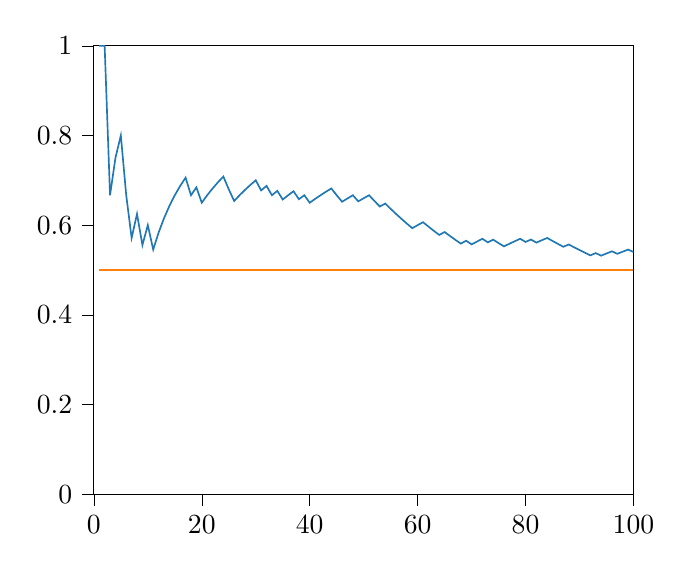
\begin{tikzpicture}
    
            \definecolor{color0}{rgb}{0.12156862745098,0.466666666666667,0.705882352941177}
            \definecolor{color1}{rgb}{1,0.498039215686275,0.0549019607843137}
            
            \begin{axis}[
            tick align=outside,
            tick pos=left,
            x grid style={white!69.0196078431373!black},
            xmin=0, xmax=100,
            xtick style={color=black},
            y grid style={white!69.0196078431373!black},
            ymin=0.0, ymax=1.0,
            ytick style={color=black}
            ]
            \addplot [semithick, color0]
            table {%
            1 1
            2 1
            3 0.666666666666667
            4 0.75
            5 0.8
            6 0.666666666666667
            7 0.571428571428571
            8 0.625
            9 0.555555555555556
            10 0.6
            11 0.545454545454545
            12 0.583333333333333
            13 0.615384615384615
            14 0.642857142857143
            15 0.666666666666667
            16 0.6875
            17 0.705882352941177
            18 0.666666666666667
            19 0.684210526315789
            20 0.65
            21 0.666666666666667
            22 0.681818181818182
            23 0.695652173913043
            24 0.708333333333333
            25 0.68
            26 0.653846153846154
            27 0.666666666666667
            28 0.678571428571429
            29 0.689655172413793
            30 0.7
            31 0.67741935483871
            32 0.6875
            33 0.666666666666667
            34 0.676470588235294
            35 0.657142857142857
            36 0.666666666666667
            37 0.675675675675676
            38 0.657894736842105
            39 0.666666666666667
            40 0.65
            41 0.658536585365854
            42 0.666666666666667
            43 0.674418604651163
            44 0.681818181818182
            45 0.666666666666667
            46 0.652173913043478
            47 0.659574468085106
            48 0.666666666666667
            49 0.653061224489796
            50 0.66
            51 0.666666666666667
            52 0.653846153846154
            53 0.641509433962264
            54 0.648148148148148
            55 0.636363636363636
            56 0.625
            57 0.614035087719298
            58 0.603448275862069
            59 0.593220338983051
            60 0.6
            61 0.60655737704918
            62 0.596774193548387
            63 0.587301587301587
            64 0.578125
            65 0.584615384615385
            66 0.575757575757576
            67 0.567164179104478
            68 0.558823529411765
            69 0.565217391304348
            70 0.557142857142857
            71 0.563380281690141
            72 0.569444444444444
            73 0.561643835616438
            74 0.567567567567568
            75 0.56
            76 0.552631578947368
            77 0.558441558441558
            78 0.564102564102564
            79 0.569620253164557
            80 0.5625
            81 0.567901234567901
            82 0.560975609756098
            83 0.566265060240964
            84 0.571428571428571
            85 0.564705882352941
            86 0.558139534883721
            87 0.551724137931034
            88 0.556818181818182
            89 0.550561797752809
            90 0.544444444444444
            91 0.538461538461538
            92 0.532608695652174
            93 0.537634408602151
            94 0.531914893617021
            95 0.536842105263158
            96 0.541666666666667
            97 0.536082474226804
            98 0.540816326530612
            99 0.545454545454545
            100 0.54
            };
            \addplot [semithick, color1]
            table {%
            1 0.5
            2 0.5
            3 0.5
            4 0.5
            5 0.5
            6 0.5
            7 0.5
            8 0.5
            9 0.5
            10 0.5
            11 0.5
            12 0.5
            13 0.5
            14 0.5
            15 0.5
            16 0.5
            17 0.5
            18 0.5
            19 0.5
            20 0.5
            21 0.5
            22 0.5
            23 0.5
            24 0.5
            25 0.5
            26 0.5
            27 0.5
            28 0.5
            29 0.5
            30 0.5
            31 0.5
            32 0.5
            33 0.5
            34 0.5
            35 0.5
            36 0.5
            37 0.5
            38 0.5
            39 0.5
            40 0.5
            41 0.5
            42 0.5
            43 0.5
            44 0.5
            45 0.5
            46 0.5
            47 0.5
            48 0.5
            49 0.5
            50 0.5
            51 0.5
            52 0.5
            53 0.5
            54 0.5
            55 0.5
            56 0.5
            57 0.5
            58 0.5
            59 0.5
            60 0.5
            61 0.5
            62 0.5
            63 0.5
            64 0.5
            65 0.5
            66 0.5
            67 0.5
            68 0.5
            69 0.5
            70 0.5
            71 0.5
            72 0.5
            73 0.5
            74 0.5
            75 0.5
            76 0.5
            77 0.5
            78 0.5
            79 0.5
            80 0.5
            81 0.5
            82 0.5
            83 0.5
            84 0.5
            85 0.5
            86 0.5
            87 0.5
            88 0.5
            89 0.5
            90 0.5
            91 0.5
            92 0.5
            93 0.5
            94 0.5
            95 0.5
            96 0.5
            97 0.5
            98 0.5
            99 0.5
            100 0.5
            };
            \end{axis}
            
            \end{tikzpicture}
    \end{center}
\noindent
En mathématiques, nous modélisons cette expérience en disant que l'univers des possibles est un
ensemble $\Omega\defeq\ens{P, F}$ formé de deux éléments  et que la probabilité de l'évènement
$A\defeq\ens{P}$ est \nicefrac{1}{2}, ce que l'on note
\[\mathbb{P}(\ens{P})=\frac{1}{2}.\]
Puisque le nombre $n_F$ de fois où on a obtenu face vérifie $n_P+n_F=n$, on en déduit que
la probabilité d'obtenir face est aussi de \nicefrac{1}{2}, ce que l'on note de même
$\mathbb{P}(\ens{F})=1/2$.\\

Considérons maintenant un autre jeu de hasard~: le lancer d'un dé à 6 faces. Dans ce cas,
l'univers des possibles est $\Omega\defeq\intere{1}{6}$. On constate que quel que
soit $\omega\in\Omega$, si on lance le dé $n$ fois et qu'on compte le nombre $n_\omega$ de
fois où on a obtenu $\omega$, la proportion $n_\omega/n$ tend vers $\nicefrac{1}{6}$. On écrira
\[\forall \omega\in\intere{1}{6}\qsep \mathbb{P}(\ens{\omega})=\frac{1}{6}.\]
Si l'on s'intéresse au nombre $n_P$ de fois où on a obtenu un nombre pair, c'est-à-dire au
nombre de fois où on a obtenu 2, 4 ou 6, nous dirons que nous nous intéressons à l'évènement
$A\defeq\ens{2,4,6}$. Bien entendu
\[\frac{n_P}{n}=\frac{n_2+n_4+n_6}{n}=\frac{n_2}{n}+\frac{n_4}{n}+\frac{n_6}{n}
  \tendvers{n}{+\infty} 3\times\frac{1}{6}=\frac{1}{2}.\]
On écrira 
\[\mathbb{P}(\ens{2, 4, 6})=\frac{1}{2}.\]
Nous remarquons que sur ces deux exemples, l'univers $\Omega$ est fini et que, quelle que soit
la partie $A$ de $\Omega$, on a
\[\mathbb{P}(A)=\frac{\card A}{\card \Omega}.\]
Nous dirons que la probabilité $\mathbb{P}$ est uniforme sur $\Omega$.\\

Cependant, les probabilités ne sont pas toujours uniformes. On considère par exemple
l'expérience
qui consiste à avoir 2 enfants. Si on s'intéresse au sexe des enfants, il y a trois
possibilités~: on peut avoir deux filles, deux garçons ou une fille et un garçon. Nous
modélisons cela en disant que l'univers des possibles est $\Omega\defeq\ens{F,G,D}$.
L'expérience montre que la probabilité d'avoir deux filles est de $\nicefrac{1}{4}$,
celle d'avoir deux garçons est de $\nicefrac{1}{4}$ et celle d'avoir une fille et un
garçon est de $\nicefrac{1}{2}$. Nous avons donc un exemple simple où la
probabilité n'est pas uniforme.\\

En 1881, l'astronome
\nom{Simon Newcomb} se rend compte que les livres de tables de logarithmes sont plus
abimés à certaines pages qu'à d'autres. Sa découverte suggère que les personnes
ayant besoin de faire des applications numériques sont plus souvent confrontées à des nombres
commençant par un 1, comme 1491 ou $1.602\times 10^{-19}$, que par un 9, comme $987$ ou $9.81$.
Soixante ans plus tard, \nom{Frank Benford}, après avoir
répertorié un très grand nombre de données, dont les longueurs des fleuves et les populations
des villes, fait le même constat. Ici, l'univers des possibles est $\Omega\defeq\intere{1}{9}$
et \nom{Benford} postule que
\[\forall \omega\in\intere{1}{9}\qsep \mathbb{P}(\ens{\omega})=\log_{10}\p{1+\frac{1}{\omega}}.\]

\begin{center}
% This file was created by tikzplotlib v0.9.8.
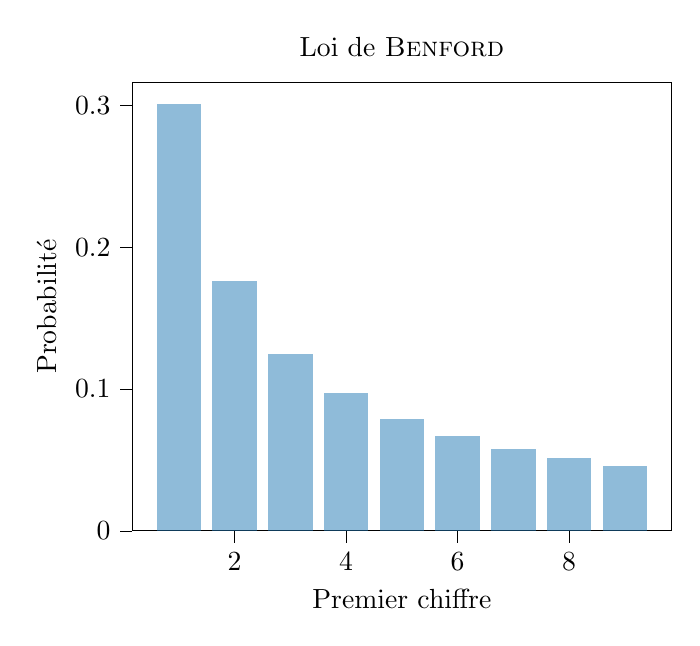
\begin{tikzpicture}

\definecolor{color0}{rgb}{0.12156862745098,0.466666666666667,0.705882352941177}

\begin{axis}[
tick align=outside,
tick pos=left,
title={Loi de \textsc{Benford}},
x grid style={white!69.0196078431373!black},
xlabel={Premier chiffre},
xmin=0.16, xmax=9.84,
xtick style={color=black},
y grid style={white!69.0196078431373!black},
ylabel={Probabilité},
ymin=0, ymax=0.31608149544718,
ytick style={color=black}
]
\draw[draw=none,fill=color0,fill opacity=0.5] (axis cs:0.6,0) rectangle (axis cs:1.4,0.301029995663981);
\draw[draw=none,fill=color0,fill opacity=0.5] (axis cs:1.6,0) rectangle (axis cs:2.4,0.176091259055681);
\draw[draw=none,fill=color0,fill opacity=0.5] (axis cs:2.6,0) rectangle (axis cs:3.4,0.1249387366083);
\draw[draw=none,fill=color0,fill opacity=0.5] (axis cs:3.6,0) rectangle (axis cs:4.4,0.0969100130080564);
\draw[draw=none,fill=color0,fill opacity=0.5] (axis cs:4.6,0) rectangle (axis cs:5.4,0.0791812460476248);
\draw[draw=none,fill=color0,fill opacity=0.5] (axis cs:5.6,0) rectangle (axis cs:6.4,0.0669467896306132);
\draw[draw=none,fill=color0,fill opacity=0.5] (axis cs:6.6,0) rectangle (axis cs:7.4,0.0579919469776867);
\draw[draw=none,fill=color0,fill opacity=0.5] (axis cs:7.6,0) rectangle (axis cs:8.4,0.0511525224473813);
\draw[draw=none,fill=color0,fill opacity=0.5] (axis cs:8.6,0) rectangle (axis cs:9.4,0.0457574905606751);
\end{axis}

\end{tikzpicture}

\end{center}
\noindent
On vérifie que
\begin{eqnarray*}
\sum_{\omega=1}^9 \mathbb{P}(\ens{\omega})
&=& \sum_{\omega=1}^9 \log_{10}\p{1+\frac{1}{\omega}}
= \sum_{\omega=1}^9 \cro{\log_{10}\p{\omega+1}-\log_{10}\p{\omega}}\\
&=& \log_{10}\p{10}-\log_{10}\p{1} = 1
\end{eqnarray*}
comme attendu pour une probabilité.\\

L'objet de la théorie des probabilités est de calculer, en fixant la probabilité de certains
évènements simples, la probabilité d'évènements plus complexes.

\subsection{Espace probabilisé}

\begin{definition}
Étant donné une expérience aléatoire, on appelle \emph{univers des possibles} ou simplement
\emph{univers} tout ensemble fini $\Omega$ où chaque élément $\omega\in\Omega$ représente une
\emph{réalisation} de l'expérience.
\end{definition}

\begin{exemples}
\exemple \emph{Série de Pile ou Face}. Soit $n\in\N$. On considère l'expérience aléatoire
  qui consiste à jeter $n$ fois une pièce. Dans ce cas, l'univers des possibles est
  $\Omega\defeq\ens{P,F}^n$, la lettre $P$ représentant le résultat pile et la lettre
  $F$ représentant le résultat face. Par exemple, si $n=3$,
  $\omega\defeq(P,P,F)$ représente la réalisation de l'expérience où les deux premiers
   lancers donnent pile et le dernier lancer donne face.
\exemple \emph{Répartition de $n$ boules discernables dans $p$ urnes discernables}. Soit
  $n,p\in\N$. On considère l'expérience qui consiste à répartir de manière aléatoire $n$
  boules discernables dans $p$ urnes discernables. On choisit de numéroter les boules de
  1 à $n$ et les urnes de $1$ à $p$. L'univers des possibles est donc
  $\Omega_D\defeq\intere{1}{p}^n$ et une réalisation $\omega\in\Omega$ de l'expérience
   est un $n$-uplet $(\omega_1,\ldots,\omega_n)$ où pour tout $i\in\intere{1}{n}$,
  $\omega_i\in\intere{1}{p}$ est le numéro de l'urne dans laquelle on a placé la boule $i$.
\exemple
  \emph{Répartition de $n$ boules indiscernables dans $p$ urnes discernables}. Soit
  $n,p\in\N$. On considère l'expérience qui consiste à répartir de manière aléatoire
  $n$ boules indiscernables dans $p$ urnes discernables. Une réalisation est
  caractérisée par le nombre de boules $x_1,\ldots,x_p\in\N$ que contient chaque urne.
  Comme on sait qu'il y a au total $n$ boules, l'univers des possibles est donc
  \[\Omega_I\defeq\enstq{(x_1,\ldots,x_p)\in\N^p}{x_1+\cdots+x_p=n}.\]
\end{exemples}

\begin{remarqueUnique}
\remarque En première année, l'univers des possibles sera toujours un ensemble fini. Cette
  restriction nous empêchera de modéliser certaines expériences comme jouer à pile ou face
  jusqu'à obtenir pile. La théorie des probabilités sur un univers infini est
  plus délicate. C'est pourquoi vous ne l'aborderez qu'en seconde année.
\end{remarqueUnique}

\begin{definition}
Soit $\Omega$ l'univers des possibles.
\begin{itemize}
\item On appelle \emph{évènement} toute partie de $\Omega$. L'évènement $\Omega$ est appelé
  \emph{évènement certain} et l'évènement $\emptyset$ est appelé \emph{évènement impossible}.
\item On dit que deux évènements $A,B\in\mathcal{P}(\Omega)$ sont
  \emph{disjoints}, ou \emph{incompatibles}, lorsque
  $A\cap B=\emptyset$.
\end{itemize}
\end{definition}

\begin{remarques}
\remarque On dit que les évènements $A_1,\ldots,A_n\in\mathcal{P}(\Omega)$ sont incompatibles
  lorsque
  \[\forall i,j\in\intere{1}{n}\qsep i\neq j\implique A_i\cap A_j=\emptyset.\]
\remarque On dit qu'un évènement $A$ est \emph{élémentaire} lorsqu'il ne contient qu'un résultat
  observable, c'est-à-dire lorsqu'il existe $\omega\in\Omega$ tel que $A=\ens{\omega}$.
\remarque Si $A$ et $B\in\mathcal{P}(\Omega)$ sont des évènements, on appelle
  \begin{itemize}
  \item évènement \og $A$ et $B$ \fg l'évènement $A\cap B$.
  \item évènement \og $A$ ou $B$ \fg l'évènement $A\cup B$.
  \item évènement \og contraire de $A$ \fg l'évènement $\bar{A}=\Omega\setminus A$.
  \end{itemize}
\end{remarques}


\begin{exoUnique}
\exo On considère l'expérience consistant à jeter $n$ fois une pièce.
  Pour tout $k\in\intere{1}{n}$, on considère l'évènement
  $F_k\defeq$ \og Le résultat du $k$-ième lancer est face \fg. Exprimer, en fonction des $F_k$,
  les évènements suivants~:
  \begin{itemize}
  \item $A\defeq$ \og On n'obtient jamais pile au cours des $n$ lancers \fg.
  \item $B\defeq$ \og On obtient pile au moins une fois au cours au cours des $n$ lancers\fg.
  \item $C\defeq$ \og On obtient deux faces consécutifs au cours des $n$ lancers \fg.
  \end{itemize}

\end{exoUnique}

% \begin{exos}
% \exo Soit $A_1,\dots,A_n$ des évènements sur un univers $\Omega$. Exprimer en fonction des
%   $A_i$ les évènements suivants.
%   \begin{itemize}
%   \item $A \defeq$ \og Tous les $A_i$ sont réalisés \fg.
%   \item $B \defeq$ \og L'un des $A_i$ est réalisé \fg.
%   \item $C \defeq$ \og Aucun des $A_i$ n'est réalisé \fg.
%   \item $D \defeq$ \og Au moins l'un des $A_i$ n'est pas réalisé \fg.
%   \item $E \defeq$ \og Un seul des $A_i$ est réalisé \fg.
%   \end{itemize}
% \begin{sol}
% \begin{enumerate}
% \item $\bigcap_{i=1}^n A_i$.
% \item $\bigcup_{i=1}^n A_i$.
% \item $\overline{\bigcup_{i=1}^n A_i}$.
% \item $\bigcup_{i=1}^n \overline{A_i}$.
% \item $\bigcup_{i=1}^n \p{(\cap_{j\neq i}^n \overline{A_j})\cap A_i}$. 
% \end{enumerate}
% \end{sol}
% \exo On tire au hasard deux cartes dans un jeu de 32 cartes
%   (as, roi, dame, valet, 10, 9, 8, 7). On considère les évènements suivants.
%   \begin{itemize}
%   \item $A \defeq$ \og les deux cartes tirées sont rouges \fg
%   \item $B \defeq$ \og les deux cartes tirées sont un valet et un dix \fg
%   \item $C \defeq$ \og les deux cartes tirées sont des personnages \fg
%   \end{itemize}
%   Décrire par des phrases les évènements suivants.
%   \[\bar{A},\quad A \cap B \cap \bar{C},\quad A \cap B \cap C\]
% \begin{sol}
% "Au moins une des cartes n'est pas rouge". "Une carte est un valet rouge et l'autre est un 10 rouge". "C'est l'évènement impossible donc on peut dire n'importe quelle phrase impossible".
% \end{sol}
% \end{exos}
  

\begin{definition}
Soit $\Omega$ l'univers des possibles. On dit que la famille d'évènements
$(A_1,\ldots,A_n)\in\mathcal{P}(\Omega)^n$ forme un \emph{système complet d'évènements}
lorsque c'est une partition de $\Omega$, c'est-à-dire lorsque
\[\Omega = \bigcup_{i=1}^n A_i \qquad\et\qquad \cro{\forall i,j\in\intere{1}{n}\qsep i\neq j\implique
  A_i\cap A_j=\emptyset}.\]
\end{definition}


% \begin{exemples}
% \exemple Dans un casino, il y a $n$ machines à sous. On choisit une machine au hasard et on
%   joue une fois sur cette machine ce qui nous donne soit gagnant, soit perdant.
%   Dans ce cas, l'univers des possibles est
%   $\Omega\defeq\intere{1}{n}\times\ens{g, p}$. Par exemple, un résultat observable de cette
%   expérience est $\omega\defeq(3,g)$; il signifie qu'un a choisi la machine 3 et qu'on a
%   gagné. Pour tout $k\in\intere{1}{n}$, on note $M_k$ l'évènement \og on a choisi la
%   $k$-ième machine \fg. D'autre part, on note $G$ l'évènement \og on a gagné \fg et $P$
%   l'évènement \og on a perdu\fg. Alors $(G,P)$ forme un système complet d'évènements. De
%   même, $(M_1,\ldots,M_n)$ forme un système complet d'évènements
% \end{exemples}

\begin{definition}
On appelle \emph{loi de probabilité}, \emph{mesure de probabilité} ou plus simplement \emph{probabilité} sur un univers $\Omega$
toute application
\[\dspappli{\mathbb{P}}{\mathcal{P}(\Omega)}{\interf{0}{1}}{A}{\mathbb{P}(A)}\]
telle que
\begin{itemize}
\item $\mathbb{P}(\Omega)=1$
\item $\forall A,B\in\mathcal{P}(\Omega)\qsep A\cap B=\emptyset \quad\implique\quad
  \mathbb{P}(A\cup B)=\mathbb{P}(A)+\mathbb{P}(B)$.
\end{itemize}
Le couple $(\Omega,\mathbb{P})$ est appelé \emph{espace probabilisé}.
\end{definition}

\begin{remarques}
\remarque On dit que deux évènements $A$ et $B$ sont \emph{équiprobables}
  lorsque $\mathbb{P}(A)=\mathbb{P}(B)$.
\remarque Si $\Omega$ est un ensemble fini non vide, l'application $\mathbb{P}$ définie par
\[\forall A\in\mathcal{P}(\Omega)\qsep \mathbb{P}(A)=\frac{\card A}{\card \Omega}.\]  
est une probabilité que nous appelerons \emph{probabilité uniforme}.
\remarque Dans la suite de ce cours, $(\Omega,\mathbb{P})$ désignera un espace probabilisé.
\end{remarques}



\begin{proposition}
\begin{eqnarray*}
\mathbb{P}(\emptyset)=0,& &\mathbb{P}(\Omega)=1,\\
\forall A\in\mathcal{P}(\Omega),& &\mathbb{P}(\bar{A})=1-\mathbb{P}(A),\\
\forall A,B\in\mathcal{P}(\Omega),& &\mathbb{P}(A\cup B)=\mathbb{P}(A)+\mathbb{P}(B)-\mathbb{P}(A\cap B).
\end{eqnarray*}
\end{proposition}

\begin{proposition}
Une probabilité est une fonction \emph{croissante}. Autrement dit
\[\forall A,B\in\mathcal{P}(\Omega)\qsep A\subset B \quad\implique\quad \mathbb{P}(A)\leq\mathbb{P}(B).\]
\end{proposition}

\begin{proposition}
Soit $(A_1,\ldots,A_n)\in\mathcal{P}(\Omega)^n$ une famille d'évènements incompatibles.
Alors
\[\mathbb{P}\p{\bigcup_{i=1}^n A_i}=\sum_{i=1}^n \mathbb{P}(A_i).\]
\end{proposition}

\begin{remarques}
\remarque Si $A_1,\ldots,A_n$ est une famille d'évènements incompatibles, la réunion des $A_i$ est parfois
  notée
  \[\bigsqcup_{i=1}^n A_i.\]
\remarque Si $A_1,\ldots,A_n$ ne sont pas incompatibles, on a seulement
  \[\mathbb{P}\p{\bigcup_{i=1}^n A_i}\leq\sum_{i=1}^n \mathbb{P}(A_i).\]
  On dit que $\mathbb{P}$ est \emph{sous-additive}. 
\end{remarques}


\begin{proposition}[nom={Formule du crible}]
Soit $(A_1,\ldots,A_n)\in\mathcal{P}(\Omega)^n$ une famille d'évènements. Alors
  \[\mathbb{P}\p{\bigcup_{i=1}^n A_n}=\sum_{k=1}^n (-1)^{k+1}
    \sum_{1\leq i_1<\cdots<i_k\leq n}
    \mathbb{P}\p{A_{i_1}\cap\cdots\cap A_{i_k}}.\]
\end{proposition}

\begin{remarqueUnique}
\remarque   Par exemple, pour $n=3$, la formule du crible s'écrit
\[\mathbb{P}\p{A_1\cup A_2\cup A_3}=\mathbb{P}(A_1)+\mathbb{P}(A_2)+\mathbb{P}(A_3) - \cro{\mathbb{P}(A_2\cap A_3)+\mathbb{P}(A_1\cap A_3)+\mathbb{P}(A_1\cap A_2)}+\mathbb{P}(A_1\cap A_2\cap A_3).\]
\end{remarqueUnique}


\begin{definition}
\begin{itemize}
\item On appelle \emph{distribution de probabilité} sur
  $\Omega$ toute famille $(p_{\omega})_{\omega\in\Omega}$ de réels positifs telle que
  \[\sum_{\omega\in\Omega} p_{\omega}=1.\]
\item Si $\mathbb{P}$ est une probabilité sur $\Omega$, on appelle \emph{distribution de
  probabilité} de $\mathbb{P}$ la famille $(p_{\omega})_{\omega\in\Omega}$ définie par
  \[\forall \omega\in\Omega\qsep p_{\omega}\defeq \mathbb{P}(\ens{\omega}).\]
  C'est une distribution de probabilité sur $\Omega$.
\end{itemize}
\end{definition}

% \begin{remarqueUnique}
% \remarque Si $(p_\omega)_{\omega\in\Omega}$ est une distribution de probabilité sur $\Omega$, on appelle support
%   de $p$ l'ensemble $\enstq{\omega\in\Omega}{p_{\omega}>0}$.
%   Par extension, le support d'une probabilité $\mathbb{P}$ est le support de sa distribution de probabilité.
%   Autrement dit
%   \[{\rm Supp}(\mathbb{P})\defeq\enstq{\omega\in\Omega}{\mathbb{P}(\ens{\omega})>0}.\]
%   % On s'intéressera le plus souvent à des espaces probabilisés $(\Omega,\mathbb{P})$
%   % pour lesquels ${\rm Supp}(\mathbb{P})=\Omega$.
% \end{remarqueUnique}

\begin{exoUnique}
\exo Sur l'univers $\Omega\defeq\intere{0}{n}$, on définit la famille $(p_k)_{0\leq k\leq n}$ par
  \[\forall k\in\intere{0}{n}\qsep p_k\defeq\alpha\binom{n}{k}\]
  où $\alpha\in\R$. Déterminer $\alpha$ pour que $(p_k)_{0\leq k\leq n}$ soit une distribution de probabilité. 
\end{exoUnique}


\begin{proposition}
Soit $(\Omega,\mathbb{P})$ un espace probabilisé et $(p_\omega)_{\omega\in\Omega}$ la distribution de probabilité de $\mathbb{P}$. Alors
\[\forall A\in\mathcal{P}(\Omega)\qsep \mathbb{P}(A)=\sum_{\omega\in A} p_{\omega}.\]
\end{proposition}

\begin{remarqueUnique}
\remarque Une probabilité est donc entièrement déterminée par sa distribution de probabilité.
% \remarque 
  % Un évènement $A$ est presque sûr si et seulement si ${\rm Supp}(\mathbb{P})\subset A$.
% \remarque En particulier, deux probabilités $\mathbb{P}_1$ et $\mathbb{P}_2$, définies sur un même univers
%   $\Omega$, sont égales si et seulement si
%   \[\forall \omega\in\Omega\qsep \mathbb{P}_1(\ens{\omega})=\mathbb{P}_2(\ens{\omega}).\]
\end{remarqueUnique}

\begin{exoUnique}
\exo On lance un dé pipé à 6 faces qui donne \og 1 \fg avec la probabilité \nicefrac{1}{4} et les
  autres faces avec une même probabilité $p$. Quelle est la probabilité d'obtenir un nombre impair~?
  \begin{sol}
  On trouve $p=3/20$, et $\mathbb{P}(Impair)=11/20$.
  \end{sol}
\end{exoUnique}

\begin{proposition}
Soit $(p_\omega)_{\omega\in\Omega}$ une distribution de probabilité sur l'univers $\Omega$. Alors il existe une
unique probabilité $\mathbb{P}$ sur $\Omega$ telle que
\[\forall \omega\in\Omega\qsep \mathbb{P}(\ens{\omega})=p_{\omega}.\]
\end{proposition}

\begin{definition}
Soit $\Omega$ un ensemble fini non vide. On appelle \emph{probabilité uniforme} sur $\Omega$
l'application $\mathbb{P}:\mathcal{P}(\Omega)\to\interf{0}{1}$ définie par
\[\forall A\in\mathcal{P}(\Omega)\qsep \mathbb{P}(A)=\frac{\card A}{\card \Omega}.\] 
\end{definition}

\begin{remarques}
\remarque Si $\mathbb{P}$ désigne la probabilité uniforme sur l'univers $\Omega$ de cardinal $n$, alors
  quel que soit $\omega\in\Omega$, $p_\omega=1/n$.
\remarque Une probabilité est uniforme si et seulement si tous les évènements élémentaires sont équiprobables.
  Une erreur très classique en probabilités est de croire que la mesure de probabilité \og naturelle \fg
  sur un univers est toujours la probabilité uniforme. Ce n'est pas toujours le cas. Cependant, lorsque ça l'est,
  un argument de symétrie permet souvent de s'en convaincre.
  Par exemple, si on lance un dé à 6 faces, les symétries du dé font que les valeurs obtenues sont
  équiprobables. La mesure de probabilité \og naturelle \fg sur $\Omega\defeq\intere{1}{6}$ est donc la probabilité
  uniforme.
\remarque Cherchons à déterminer les probabilités \og naturelles \fg sur les 3 exemples que nous avons
  donnés en début de cours.
  \begin{itemize}
  \item \emph{Série de Pile ou Face}~: Si on considère l'expérience aléatoire qui consiste à jeter $n$ fois une
    pièce équilibrée, on se convaincra que tous les évènements élémentaires sont équiprobables. C'est donc la
    probabilité uniforme qui est naturelle sur l'univers $\Omega\defeq\ens{P,F}^n$. Nous verrons plus tard que cela
    revient à supposer que les
    résultats de chaque lancer ont autant de chance de donner pile que face, et que les lancers sont indépendants.
  \item \emph{Répartition de $n$ boules discernables dans $p$ urnes discernables}~: Si l'on souhaite répartir
    $n$ boules discernables dans $p$ urnes discernables, on se convaincra aussi que la probabilité naturelle est
    la probabilité uniforme sur $\Omega_D\defeq\intere{1}{p}^n$. Nous verrons que cela revient à supposer que chaque
    boule soit placée de manière équiprobable dans les urnes et que ces répartitions sont indépendantes les unes
    des autres.
  \item \emph{Répartition de $n$ boules indiscernables dans $p$ urnes discernables}~: Enfin, si l'expérience
    est de répartir $n$ boules indiscernables dans $p$ urnes discernables, la probabilité naturelle n'est
    plus la probabilité uniforme. Pour s'en convaincre, on peut essayer de comprendre ce qui se passe pour
    $n=2$ et $p=2$. On considère donc l'expérience qui consiste à placer deux boules indiscernables dans 2 urnes
    distinctes. Il y a 3 réalisations possibles de cette expérience~: \og Les deux boules sont dans la première urne \fg,
    \og Les deux boules sont dans la seconde urne\fg et \og Il y a une boule dans chaque urne\fg. L'univers des possibles
    $\Omega_I$ possède donc 3 éléments. On se convaincra facilement que l'évènement \og Il y a une boule dans
    chaque urne \fg a une probabilité naturelle de \nicefrac{1}{2}. En effet, une fois que la première boule est placée,
    on a une chance sur deux que la seconde boule soit placée dans la même urne. Les probabilités naturelles
    pour cette expérience sont donc respectivement de \nicefrac{1}{4}, \nicefrac{1}{4} et \nicefrac{1}{2}, ce
    qui ne dérive pas d'une loi uniforme. Pour traiter ce type de problème, on peut considérer que
    les boules sont discernables et travailler sur $\Omega_D$ muni de la probabilité uniforme.
  \end{itemize}
\remarque Lorsque $\Omega$ est muni d'une loi uniforme, les calculs de probabilité se ramènent donc à des
  problèmes de dénombrement.
\end{remarques}

\begin{exos}
  \exo Une urne contient 20 boules~: 5 boules blanches, 5 boules rouges, 10 boules noires.
  % \begin{questions}
  % \question
  On tire 3 boules, successivement et avec remise à chaque tirage. Calculer la probabilité que
    le tirage soit~:
    \begin{itemize}
  \item tricolore.
  \item bicolore.
  \item unicolore.
    \end{itemize}
  % \question On tire 3 boules simultanément. Reprendre les questions précédentes.
  % \end{questions}
  \begin{sol}
  \begin{questions}
  \question $\Card\Omega=20^3=8000$~: ce sont des triplets de $\intere{1}{20}$. La loi de probabilité est uniforme.
    \begin{itemize}
    \item $\Card A=10\times 5\time 5\times 3!$. On trouve une probabilité de $3/16$.
    \item $\Card B=375+375+1500+750+1500+750$. On troube une proba de $21/32$.
    \item $\Card C=125+!25+1000$. On trouve une proba de $5/32$.
    \end{itemize}
  \question $\Card\Omega=\binom{20}{3}=1440$.
    \begin{itemize}
    \item $250$, puis $25/114$.
    \item $25/38$.
    \item $7/57$.
    \end{itemize}
  \end{questions}
  \end{sol}
  \exo Une urne contient 3 boules blanches et 5 noires. On en tire simultanément 4 boules.
    Avec quelle probabilité n'a-t-on tiré que des boules noires~?
    \begin{sol}
    On trouve (4 parmi 5)/(4 parmi 8) et donc \nicefrac{1}{14}.
    \end{sol}
\end{exos}

% \begin{remarques}
% \remarque On considère l'expérience aléatoire qui consiste à lancer une pièce. L'univers
%   des possibles est $\Omega\defeq\ens{P,F}$, la lettre $P$ représentant le résultat pile,
%   et la lettre $F$ représentant le résultat face. Si la pièce est équilibrée, l'expérience
%   montre que la probabilité d'obtenir une pile est de \nicefrac{1}{2} et la probabilité
%   d'obtenir un face est de \nicefrac{1}{2}. C'est bien la probabilité
%   uniforme sur $\Omega$. 
% \remarque On considère l'expérience aléatoire qui consiste à lancer un dé à 6 faces.
%   L'univers des possibles est $\Omega\defeq\intere{1}{6}$. Si le dé n'est pas pipé,
%   l'expérience montre que quel que soit $\omega\in\intere{1}{6}$, la probabilité d'obtenir
%   $\omega$ est de \nicefrac{1}{6}. La probabilité naturelle sur $\Omega$ est donc la
%   probabilité uniforme.
% \remarque Soit $n\in\N$. On considère l'expérience aléatoire qui consiste à lancer $n$
%   fois une pièce. L'univers des possibles est donc $\Omega\defeq\ens{P,F}^n$.
%   En supposant que la probabilité d'obtenir un pile à chaque lancer est de \nicefrac{1}{2} et
%   que les lancers sont mutuellements indépendants, nous démontrerons plus tard que tous les
%   résultats sont équiprobables. La probabilité naturelle sur $\Omega$ est donc la probabilité
%   uniforme.
% \remarque Soit $n,p\in\N$. On considère l'expérience aléatoire qui consiste à placer $n$
%   boules discernables dans $p$ urnes discernables. En numérotant les boules de 1 à $n$ et
%   les urnes de 1 à $p$, l'univers des possibles est
%   $\Omega\defeq\mathcal{F}(\intere{1}{n},\intere{1}{p})$, un résultat observable étant une
%   application $\omega\in\Omega$ qui a une boule $i\in\intere{1}{n}$ associe l'urne $\omega(i)\in\intere{1}{p}$
%   dans laquelle elle a été placée. En supposant que les boules sont placées les unes
%   après les autres avec une probabilité uniforme sur toutes les urnes et qu'elle sont placées
%   de manière indépendante, nous démontrerons plus tard que tous les résultats sont
%   équiprobables. La probabilité naturelle sur $\Omega$ est donc la probabilité
%   uniforme.
% \end{remarques}

% \begin{proposition}
% Soit $\Omega=\ens{\omega_1,\ldots,\omega_n}$ un ensemble fini de cardinal $n$ et
% $p_1,\ldots,p_n\in\RP$ tels que $p_1+\cdots+p_n=1$. Alors il existe une unique
% mesure de probabiblité $\mathbb{P}$ sur $\Omega$ telle que
% \[\forall i\in\intere{1}{n}\qsep \mathbb{P}(\ens{\omega_i})=p_i.\]
% \end{proposition}



% \begin{definition}
% Soit $(\Omega,\mathbb{P})$ un espace probabilisé, $\Omega'$ un ensemble fini et
% $f:\Omega\to\Omega'$. Alors l'application
% \[\dspappli{\mathbb{P}_f}{\mathcal{P}(\Omega')}{\interf{0}{1}}{A}{\mathbb{P}\p{f^{-1}(A)}}\]
% est une probabilité sur $\Omega'$, appelée \emph{mesure image} de $\mathbb{P}$ par $f$.
% \end{definition}



% Ici, il faut parler de boules discernables et indiscernables.

% \begin{remarqueUnique}
% \remarque Soit $n,p\in\N$. On considère l'expérience aléatoire qui consiste à placer $n$
%   boules indiscernables dans $p$ urnes discernables. On note $\Omega$ l'univers des
%   possibles. Pour définir une probabilité
%   naturelle sur $\Omega$, il est bon de commencer par imaginer que les boules sont
%   discernables. Cela nous conduit à considérer l'univers $\Omega_1\defeq\mathcal{F}(\intere{1}{n},\intere{1}{p})$
%   muni de la probabilité uniforme $\mathbb{P}_1$. 
%   %  En numérotant les boules de 1 à $n$ et
%   % les urnes de 1 à $p$, l'univers des possibles est
%   % $\Omega\defeq\mathcal{F}(\intere{1}{n},\intere{1}{p})$, un résultat observable étant une
%   % application $\omega\in\Omega$ qui a une boule $i\in\intere{1}{n}$ associe l'urne $\omega(i)\in\intere{1}{p}$
%   % dans laquelle elle a été placée. En supposant que les boules sont placées les unes
%   % après les autres avec une probabilité uniforme sur toutes les urnes et qu'elle sont placées
%   % de manière indépendante, nous démontrerons plus tard que tous les résultats sont
%   % équiprobables. La probabilité naturelle sur $\Omega$ est donc la probabilité
%   % uniforme.
% \end{remarqueUnique}

\subsection{Variable aléatoire}

\begin{definition}
Soit $(\Omega,\mathbb{P})$ un espace probabilisé. On appelle \emph{variable aléatoire}
à valeurs dans $E$ toute application $X:\Omega\to E$.
\end{definition}

\begin{remarqueUnique}
\remarque On dit qu'une variable aléatoire $X:\Omega\to E$ est réelle lorsque $E$ est une
  partie de $\R$.
% \remarque Puisque $\Omega$ est fini, $X(\Omega)$ est fini. Si $E'$ est une partie finie de $E$
%   telle que $X(\Omega)\subset E'$, on se permettra de confondre $X$ et sa corestriction
%   à $E'$. On pourra donc se ramener au cas où $E$ est fini.
\end{remarqueUnique}

\begin{definition}
Soit $X:\Omega\to E$ une variable aléatoire. Alors, pour toute partie $A$ de $E$, on définit
l'évènement
\[(X\in A)\defeq\enstq{\omega\in\Omega}{X(\omega)\in A}.\] 
\end{definition}

\begin{remarques}
\remarque Si $x\in E$, l'évènement $\enstq{\omega\in\Omega}{X(\omega)=x}$ est noté
  $(X=x)$.
\remarque Si $X$ est une variable aléatoire réelle et $a,b\in\R$, l'évènement
  $\enstq{\omega\in\Omega}{a\leq X(\omega)\leq b}$ est noté $(a\leq X\leq b)$. 
\remarque L'évènement $(X\in A)$ est aussi noté $\ens{X\in A}$, ou $[X\in A]$. La probabilité
  d'un tel évènement est notée $\mathbb{P}(X\in A)$.
\end{remarques}

\begin{proposition}
Soit $X:\Omega\to E$ une variable aléatoire et $A,B\in\mathcal{P}(E)$. Alors
\[(X\in A\cap B)=(X\in A)\cap(X\in B), \qquad (X\in A\cup B)=(X\in A)\cup(X\in B),\]
\[(X\in \bar{A})=\overline{(X\in A)}.\]
\end{proposition}

\begin{exoUnique}
\exo Soit $X:\Omega\to\Z$ une variable aléatoire à valeurs entières. Montrer que
  \[\forall n\in\Z\qsep \mathbb{P}(X=n)=\mathbb{P}(X\leq n) - \mathbb{P}(X\leq n-1).\]
% \exo Soit $X$ une variable aléatoire réelle. Montrer que
%   $\mathbb{P}(X\leq 1)\leq \mathbb{P}(\abs{X-2}\geq 1)$.
% \exo On joue $n\in\Ns$ fois à pile ou face avec une pièce équilibrée. On compte le nombre
%   de lancers nécessaires $X$ pour obtenir pile pour la première fois. Si on obtient que des
%   faces, on pose $X=n+1$.
%   \begin{questions}
%   \question Modéliser l'expérience en précisant l'univers des possibles $\Omega$ et donner
%     une probabilité naturelle sur $\Omega$.
%   \question Pour tout $k\in\intere{0}{n}$, calculer $\mathbb{P}(X>k)$.
%   \question En déduire $\mathbb{P}(X=k)$ pour tout $k\in\intere{1}{n+1}$.
%   \end{questions}
\end{exoUnique}


\begin{definition}
Soit $X:\Omega\to E$ une variable aléatoire. Alors l'application
\[\dspappli{\mathbb{P}_X}{\mathcal{P}(X(\Omega))}{\interf{0}{1}}{A}{\mathbb{P}\p{X\in A}}\]
est une probabilité sur $X(\Omega)$, appelée \emph{loi} de $X$.
\end{definition}

\begin{remarques}
\remarque La loi de $X$ est entièrement déterminée par
  sa distribution de probabilité $(\mathbb{P}(X=x))_{x\in X(\Omega)}$.
\remarque Si $x\in E$ n'appartient pas à $X(\Omega)$, alors $\mathbb{P}(X=x)=0$.
\remarque En pratique, lorsqu'il nous sera demandé de déterminer la loi d'une variable aléatoire
  $X:\Omega\to E$, on commencera par déterminer un ensemble fini $E'$ tel que $X(\Omega)\subset E'$
  puis on calculera $\mathbb{P}(X=x)$ pour tout $x\in E'$.
\remarque Si $(\Omega_1,\mathbb{P}_1)$ est un espace probabilisé, $\Omega_2$ est un ensemble fini et
  $F$ est une application de $\Omega_1$ dans $\Omega_2$, alors
  \[\dspappli{\mathbb{P}_2}{\mathcal{P}(\Omega_2)}{\interf{0}{1}}{A}{\mathbb{P}_1\p{F\in A}}\] 
  est une probabilité sur $\Omega_2$, appelée \emph{mesure image} de $\mathbb{P}_1$ par $F$. 
  En reprenant les notations utilisées dans les exemples de répartition de $n$ boules  
  discernables/indiscernables
  dans $p$ urnes discernables donnés plus haut, 
  on considère la fonction d'oubli $F:\Omega_D\to\Omega_I$. À une répartition de boules numérotées et donc discernables, elle associe
  la répartition
  des boules indiscernables, où on a effacé le numéro des boules. Autrement dit, si
  $\omega\defeq(\omega_1,\ldots,\omega_n)\in\Omega_D$, alors
  $F(\omega)=(x_1,\ldots,x_p)\in\Omega_I$ où
  \[\forall j\in\intere{1}{p}\qsep x_j=\card\enstq{i\in\intere{1}{n}}{\omega_i=j}.\]
  La mesure de probabilité naturelle sur $\Omega_I$ est la mesure image par $F$ de la probabilité uniforme sur
  $\Omega_D$.
\end{remarques}

% \begin{remarques}
% % \remarque Le \emph{support de la variable aléatoire $X$} est défini comme étant le support
% %   de $\mathbb{P}_X$. Autrement dit
% %   \[{\rm Supp}(X)\defeq\enstq{x\in E}{\mathbb{P}(X=x)>0}.\]
% %   Remarquons que ${\rm Supp}(X)\subset X(\Omega)$, l'inclusion pouvant être stricte.
% \remarque Si l'on souhaite définir la loi d'une variable aléatoire $X:\Omega\to E$ à
%   valeurs dans un ensemble infini $E$, il suffit de considérer la corestriction
%   de $X$ à l'ensemble fini $E'\defeq X(\Omega)$. Étant donné que la détermination
%   exacte de $X(\Omega)$ nécessite parfois de traiter de nombreux
%   cas particuliers, nous nous contenterons de corestreindre $X$ à un ensemble fini $E'$ tel
%   que $X(\Omega)\subset E'$. Par exemple, si
%   $A\in\mathcal{P}(\Omega)$ et $X:\Omega\to\R$ est la fonction indicatrice
%   \[\dspappli{X}{\Omega}{\R}{\omega}{
%   \begin{cases}
%   1 & \text{si $\omega\in A$}\\
%   0 & \text{si $\omega\not\in A$.}
%   \end{cases}}\]
%   Alors $X(\Omega)\subset\ens{0,1}$. Cette inclusion est une égalité, sauf dans les cas
%   particuliers où $A=\emptyset$ et $A=\Omega$, pour lesquels $X(\Omega)$ est
%   respectivement égal à $\ens{0}$ et à $\ens{1}$. Pour une telle variable aléatoire,
%   on choisit $E'\defeq\ens{0,1}$. La distribution de probabilité $(p_0,p_1)$ de
%   $\mathbb{P}_X$ est alors donnée par
%   \[p_0=1-\mathbb{P}(A) \et p_1=\mathbb{P}(A).\]
%   Le plus souvent, on confondra $E'$ et $X(\Omega)$ et on écrira abusivement
%   $X(\Omega)=\ens{0,1}$.

% \end{remarques}

\begin{exoUnique}
\exo On lance successivement deux dés à 6 faces. On modélise cette expérience en choisissant $\Omega\defeq\intere{1}{6}^2$
  muni de la probabilité uniforme. On note $A_1:\Omega\to\N$ le résultat du premier dé et
  $A_2:\Omega\to\N$ le résultat du second dé. Déterminer les lois de $A_1$, $A_2$ ainsi que
  la loi de la variable aléatoire $A_1+A_2:\Omega\to\N$ donnant la somme des deux nombres
  obtenus.
\end{exoUnique}


% \begin{remarqueUnique}
  % Pour s'en convaincre, on considère l'expérience aléatoire qui consiste à jouer 2
  % fois à pile ou face. On modèlise cette expérience en posant $\Omega\defeq\ens{P,F}^2$ que
  % l'on munit de la probabilité uniforme. Soit $X_1:\Omega\to\ens{P,F}$ et
  % $X_2:\Omega\to\ens{P,F}$ les variables aléatoires donnant respectivement les résultats des
  % premiers et seconds lancers.  Alors $X_1$ et $X_2$ suivent la même loi. Pourtant, elles ne
  % sont pas égales.
% \end{remarqueUnique}

  
\begin{proposition}
Soit $X:\Omega\to E$ une variable aléatoire. Alors, pour toute partie $A$ de $E$
  \[\mathbb{P}(X\in A)=\sum_{x\in A} \mathbb{P}(X=x)\]
\end{proposition}

\begin{remarqueUnique}
\remarque Étant donné que $\mathbb{P}(X=x)$ est nul pour tout $x$ en dehors de l'ensemble
  fini $X(\Omega)$, cette somme est bien définie puisqu'elle ne comporte qu'un nombre fini
  de termes non nuls.
\end{remarqueUnique}


\begin{definition}
On dit que deux variables aléatoires $X,Y:\Omega\to E$ suivent la même
loi lorsque
\[\forall A\in\mathcal{P}(E)\qsep \mathbb{P}(X\in A)=\mathbb{P}(Y\in A).\]
Si tel est le cas, on écrit $X\sim Y$.
\end{definition}

\begin{remarques}
\remarque En pratique, pour montrer que $X$ et $Y$ suivent la même loi, il suffit de déterminer
  un ensemble fini $E'$ tel que $X(\Omega)\subset E'$ et $Y(\Omega)\subset E'$, puis de
  montrer que
  \[\forall a\in E'\qsep \mathbb{P}(X=a)=\mathbb{P}(Y=a).\]
\remarque Deux variables aléatoires qui suivent la même loi ne sont en général pas égales.
  Par exemple, si $A$ est un évènement de probabilité \nicefrac{1}{2}, les variables
  aléatoires $\mathds{1}_A$ et $\mathds{1}_{\bar{A}}$ suivent la même loi sans être
  égales.
\end{remarques}

\begin{proposition}
Si $X:\Omega\to E$ une variable aléatoire, $X(\Omega)$ est un ensemble fini que l'on
note $\ens{x_1,\ldots,x_n}$. Alors, la famille des $(X=x_i)$ pour $i\in\intere{1}{n}$ forme
un système complet d'évènements.
\end{proposition}

\begin{remarques}
\remarque On utilisera souvent ce système complet d'évènements dans la formule des
  probabilités totales.
\remarque Cette proposition reste vraie si on remplace $X(\Omega)$ par une partie finie
  $E'$ de $E$ telle que $X(\Omega)\subset E'$.
\end{remarques}


\begin{definition}
Soit $X:\Omega\to E$ une variable aléatoire et $f:E\to F$. On note $f(X)$ la variable
aléatoire $f\circ X:\Omega\to F$.
\end{definition}

\begin{remarqueUnique}
\remarque
Soit $X:\Omega\to E$ une variable aléatoire et $f:E\to F$. Alors, pour tout
$y\in F$
\[\mathbb{P}(f(X)=y)=\sum_{\substack{x\in X(\Omega)\\f(x)=y}} \mathbb{P}(X=x)\]
cette formule restant vraie si l'on remplace $X(\Omega)$ par une partie finie $E'$ de $E$
telle que $X(\Omega)\subset E'$.
\end{remarqueUnique}


\begin{proposition}
Soit $X,Y:\Omega\to E$ deux variables aléatoires et $f:E\to F$. Si $X\sim Y$, alors
$f(X)\sim f(Y)$.
\end{proposition}



\subsection{Lois usuelles}

% \begin{definition}[nom={Variable aléatoire constante}]
% On dit qu'une variable aléatoire $X:\Omega\to E$ est \emph{constante} lorsqu'il existe $a\in E$ tel
% que
% \[\mathbb{P}(X=a)=1.\]
% \end{definition}

% \begin{remarques}
% % \remarque Si $X:\Omega\to E$ est une variable aléatoire constante, il existe un unique
% %   $a\in E$ tel que $\mathbb{P}(X=a)=1$; on dit que $X$ est une variable aléatoire
% %   constante égale à $a$.
% % \remarque Une variable aléatoire $X:\Omega\to E$ est constante égale à $a\in E$, si et
% %   seulement si il existe un évènement presque sûr $A$ tel que
% %   \[\forall\omega\in A\qsep X(\omega)=a.\]
% \remarque Si $X:\Omega\to E$ est constante égale à $a$, alors
%   \[\forall x\in E\qsep \mathbb{P}(X=x)=
%   \begin{cases}
%   1 & \text{si $x=a$,}\\
%   0 & \text{sinon.}
%   \end{cases}\]
%   En particulier, ${\rm Supp}(\mathbb{P}_X)=\ens{a}$. On écrira parfois abusivement $X(\Omega)=\ens{a}$.
% \remarque Une variable aléatoire $X:\Omega\to E$ est constante si et seulement si il existe $a\in E$ et
%   un évènement presque sûr $A$ tel que
%   \[\forall \omega\in A\qsep X(\omega)=a.\]
% \end{remarques}


\begin{definition}[nom={Loi uniforme}]
Soit $A$ un ensemble fini non vide. On dit qu'une variable aléatoire $X$ à valeurs dans $A$
suit une \emph{loi uniforme} sur $A$ lorsque
\[\forall a\in A\qsep \mathbb{P}(X=a)=\frac{1}{\card A}.\]
Si tel est le cas, on note $X\sim\mathcal{U}(A)$.
\end{definition}

\begin{remarqueUnique}
\remarque Si $X$ suit une loi uniforme sur $A$, alors $X(\Omega)=A$.
\end{remarqueUnique}
% \begin{remarqueUnique}
% \remarque $X:\Omega\to A$ suit une loi uniforme sur $A$
% %   si et seulement si $\mathbb{P}_X$ est la probabilité uniforme sur $A$.
% \remarque Si $X:\Omega\to E$ suit une loi uniforme sur $A$, alors
%   \[\forall x\in E\qsep \mathbb{P}(X=x)=
%   \begin{cases}
%   \frac{1}{\card A} & \text{si $x\in A$,}\\
%   0 & \text{sinon.}
%   \end{cases}\]
%   En particulier, ${\rm Supp}(\mathbb{P}_X)=A$. On écrira parfois abusivement $X(\Omega)=A$.
% \end{remarqueUnique}
% \vspace{1ex}
\begin{exoUnique}
\exo Soit $X$ une variable aléatoire suivant une loi uniforme sur $\intere{-2}{2}$. Déterminer la loi
  de $X^2+1$.
\end{exoUnique}


\begin{definition}[nom={Loi de \nom{Bernoulli}}]
Soit $p\in[0,1]$. On dit qu'une variable aléatoire $X$ à valeurs dans $\ens{0,1}$ suit la \emph{loi de
\nom{Bernoulli}} de paramètre $p$ lorsque
\[\mathbb{P}(X=1)=p.\]
Si tel est le cas, $\mathbb{P}(X=0)=1-p$ et on note $X\sim\mathcal{B}(p)$.
\end{definition}

\begin{remarques}
\remarque Si $p\in[0,1]$, il est courant de poser $q\defeq 1-p\in[0,1]$.
% \remarque On a ${\rm Supp}(\mathbb{P}_X)\subset\ens{0,1}$, cette inclusion étant une
%   égalité si et seulement si $p\in]0,1[$.
%   On écrira parfois abusivement $X(\Omega)=\ens{0,1}$.
\remarque Si $X$ suit une loi de Bernoulli de paramètre $p\in]0,1[$, alors $X(\Omega)=\ens{0,1}$.
\remarque Toute variable aléatoire $X$ à valeurs dans $\ens{0,1}$ suit une loi de \nom{Bernoulli}
  de paramètre $p\defeq\mathbb{P}(X=1)$. En particulier, si $A\in\mathcal{P}(\Omega)$ est un évènement,
  alors $\mathds{1}_A$ est une variable aléatoire qui suit une
  loi de \nom{Bernoulli} de paramètre $p\defeq\mathbb{P}(A)$.
% \remarque Une loi de $\nom{Bernoulli}$ est constante si et seulement si $p=0$ ou $p=1$.
\remarque On dit qu'une variable aléatoire $Y$ à valeurs dans $\ens{-1,1}$ suit une loi de
  \nom{Rademacher} lorsque
  \[\mathbb{P}(Y=-1)=\frac{1}{2} \quad\et\quad \mathbb{P}(Y=1)=\frac{1}{2}.\]
  % Une variable aléatoire $Y$ suit une loi de \nom{Rademacher} si et seulement si il existe
  % une variable aléatoire $X$ suivant une loi de \nom{Bernoulli} de paramètre \nicefrac{1}{2}
  % telle que $Y=-1+2X$.
\end{remarques}

\begin{exempleUnique}
\exemple On considère l'expérience aléatoire d'un tir de penalty dans un match de foot. 
  La variable aléatoire $X:\Omega\to\ens{0,1}$ décrit le résultat de ce tir~: 1 si le
  penalty est réussi et 0 si le penalty est manqué. $X$ suit donc une loi de
  \nom{Bernoulli} dont le paramètre $p$ est estimé, selon les joueurs, entre $70\%$ et $90\%$.
\end{exempleUnique}

\begin{definition}[nom={Loi binomiale}]
Soit $n\in\N$ et $p\in[0,1]$. On dit qu'une variable aléatoire $X$ à valeurs dans $\intere{0}{n}$
suit la \emph{loi binomiale} de paramètre $(n,p)$ lorsque
\[\forall k\in\intere{0}{n}\qsep \mathbb{P}(X=k)=\binom{n}{k}p^k(1-p)^{n-k}.\]
Si tel est le cas, on note $X\sim\mathcal{B}(n,p)$. 
\end{definition}

\begin{remarques}
\remarque La loi binomiale $\mathcal{B}(1,p)$ n'est autre
  que la loi de \nom{Bernoulli} de paramètre $p$.
% \remarque On a ${\rm Supp}(\mathbb{P}_X)\subset\intere{0}{n}$, cette inclusion étant une
%   égalité si et seulement si $p\in ]0,1[$.
%   On écrira parfois abusivement $X(\Omega)=\intere{0}{n}$.
\remarque Si $X$ suit une loi binomiale de paramètre $(n,p)$ où $p\in]0,1[$, alors $X(\Omega)=\intere{0}{n}$.
\end{remarques}


% from scipy.special import binom
% import matplotlib.pyplot as plt
% import tikzplotlib as tikz
% n = 10
% p = 0.2
% r = [binom(n, k) * p**k * (1-p)**(n-k) for k in range(n)]
% plt.bar(range(n), r, alpha=0.5)
% tikz.save('/Users/fayard/Desktop/binomial-10.tex')

\begin{center}
% This file was created by tikzplotlib v0.9.8.
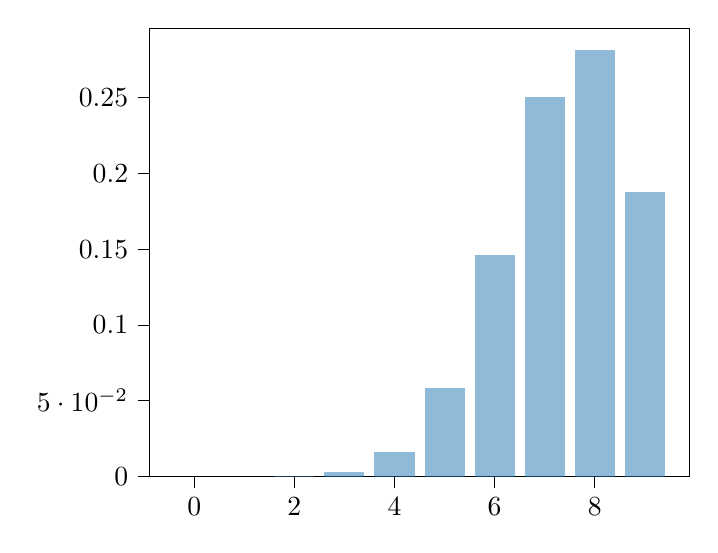
\begin{tikzpicture}

\definecolor{color0}{rgb}{0.12156862745098,0.466666666666667,0.705882352941177}

\begin{axis}[
tick align=outside,
tick pos=left,
x grid style={white!69.0196078431373!black},
xmin=-0.89, xmax=9.89,
xtick style={color=black},
y grid style={white!69.0196078431373!black},
ymin=0, ymax=0.295645952224731,
ytick style={color=black}
]
\draw[draw=none,fill=color0,fill opacity=0.5] (axis cs:-0.4,0) rectangle (axis cs:0.4,9.5367431640625e-07);
\draw[draw=none,fill=color0,fill opacity=0.5] (axis cs:0.6,0) rectangle (axis cs:1.4,2.86102294921875e-05);
\draw[draw=none,fill=color0,fill opacity=0.5] (axis cs:1.6,0) rectangle (axis cs:2.4,0.000386238098144531);
\draw[draw=none,fill=color0,fill opacity=0.5] (axis cs:2.6,0) rectangle (axis cs:3.4,0.00308990478515625);
\draw[draw=none,fill=color0,fill opacity=0.5] (axis cs:3.6,0) rectangle (axis cs:4.4,0.0162220001220703);
\draw[draw=none,fill=color0,fill opacity=0.5] (axis cs:4.6,0) rectangle (axis cs:5.4,0.0583992004394531);
\draw[draw=none,fill=color0,fill opacity=0.5] (axis cs:5.6,0) rectangle (axis cs:6.4,0.145998001098633);
\draw[draw=none,fill=color0,fill opacity=0.5] (axis cs:6.6,0) rectangle (axis cs:7.4,0.250282287597656);
\draw[draw=none,fill=color0,fill opacity=0.5] (axis cs:7.6,0) rectangle (axis cs:8.4,0.281567573547363);
\draw[draw=none,fill=color0,fill opacity=0.5] (axis cs:8.6,0) rectangle (axis cs:9.4,0.187711715698242);
\end{axis}

\end{tikzpicture}

% This file was created by tikzplotlib v0.9.8.
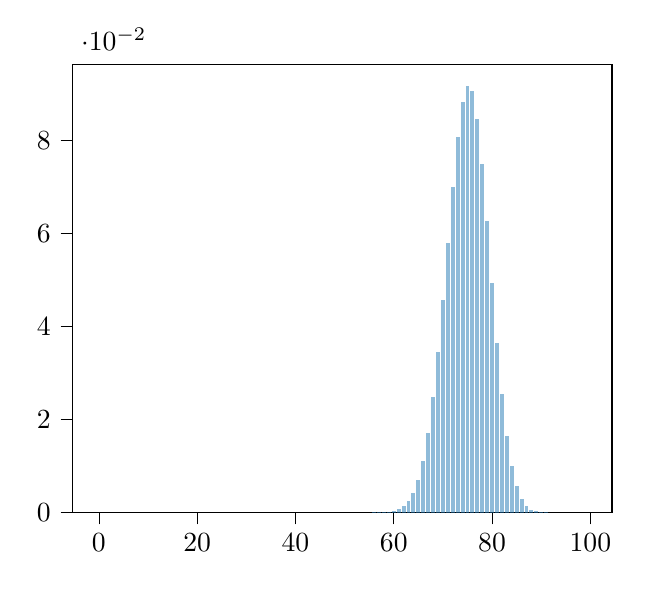
\begin{tikzpicture}

\definecolor{color0}{rgb}{0.12156862745098,0.466666666666667,0.705882352941177}

\begin{axis}[
tick align=outside,
tick pos=left,
x grid style={white!69.0196078431373!black},
xmin=-5.39, xmax=104.39,
xtick style={color=black},
y grid style={white!69.0196078431373!black},
ymin=0, ymax=0.0963896763551786,
ytick style={color=black}
]
\draw[draw=none,fill=color0,fill opacity=0.5] (axis cs:-0.4,0) rectangle (axis cs:0.4,6.22301527786114e-61);
\draw[draw=none,fill=color0,fill opacity=0.5] (axis cs:0.6,0) rectangle (axis cs:1.4,1.86690458335834e-58);
\draw[draw=none,fill=color0,fill opacity=0.5] (axis cs:1.6,0) rectangle (axis cs:2.4,2.77235330628714e-56);
\draw[draw=none,fill=color0,fill opacity=0.5] (axis cs:2.6,0) rectangle (axis cs:3.4,2.7169062401614e-54);
\draw[draw=none,fill=color0,fill opacity=0.5] (axis cs:3.6,0) rectangle (axis cs:4.4,1.97654928971742e-52);
\draw[draw=none,fill=color0,fill opacity=0.5] (axis cs:4.6,0) rectangle (axis cs:5.4,1.13849239087723e-50);
\draw[draw=none,fill=color0,fill opacity=0.5] (axis cs:5.6,0) rectangle (axis cs:6.4,5.40783885666685e-49);
\draw[draw=none,fill=color0,fill opacity=0.5] (axis cs:6.6,0) rectangle (axis cs:7.4,2.17858651082864e-47);
\draw[draw=none,fill=color0,fill opacity=0.5] (axis cs:7.6,0) rectangle (axis cs:8.4,7.5978204565149e-46);
\draw[draw=none,fill=color0,fill opacity=0.5] (axis cs:8.6,0) rectangle (axis cs:9.4,2.32999827333124e-44);
\draw[draw=none,fill=color0,fill opacity=0.5] (axis cs:9.6,0) rectangle (axis cs:10.4,6.36089528619427e-43);
\draw[draw=none,fill=color0,fill opacity=0.5] (axis cs:10.6,0) rectangle (axis cs:11.4,1.56131066115678e-41);
\draw[draw=none,fill=color0,fill opacity=0.5] (axis cs:11.6,0) rectangle (axis cs:12.4,3.47391622107383e-40);
\draw[draw=none,fill=color0,fill opacity=0.5] (axis cs:12.6,0) rectangle (axis cs:13.4,7.05472217202685e-39);
\draw[draw=none,fill=color0,fill opacity=0.5] (axis cs:13.6,0) rectangle (axis cs:14.4,1.31520177635643e-37);
\draw[draw=none,fill=color0,fill opacity=0.5] (axis cs:14.6,0) rectangle (axis cs:15.4,2.26214705533307e-36);
\draw[draw=none,fill=color0,fill opacity=0.5] (axis cs:15.6,0) rectangle (axis cs:16.4,3.60529686943707e-35);
\draw[draw=none,fill=color0,fill opacity=0.5] (axis cs:16.6,0) rectangle (axis cs:17.4,5.34432241822437e-34);
\draw[draw=none,fill=color0,fill opacity=0.5] (axis cs:17.6,0) rectangle (axis cs:18.4,7.39297934521038e-33);
\draw[draw=none,fill=color0,fill opacity=0.5] (axis cs:18.6,0) rectangle (axis cs:19.4,9.57196273116712e-32);
\draw[draw=none,fill=color0,fill opacity=0.5] (axis cs:19.6,0) rectangle (axis cs:20.4,1.1629934718368e-30);
\draw[draw=none,fill=color0,fill opacity=0.5] (axis cs:20.6,0) rectangle (axis cs:21.4,1.32913539638492e-29);
\draw[draw=none,fill=color0,fill opacity=0.5] (axis cs:21.6,0) rectangle (axis cs:22.4,1.4318413133783e-28);
\draw[draw=none,fill=color0,fill opacity=0.5] (axis cs:22.6,0) rectangle (axis cs:23.4,1.45674290143705e-27);
\draw[draw=none,fill=color0,fill opacity=0.5] (axis cs:23.6,0) rectangle (axis cs:24.4,1.40211504263316e-26);
\draw[draw=none,fill=color0,fill opacity=0.5] (axis cs:24.6,0) rectangle (axis cs:25.4,1.27872891888145e-25);
\draw[draw=none,fill=color0,fill opacity=0.5] (axis cs:25.6,0) rectangle (axis cs:26.4,1.1065923336474e-24);
\draw[draw=none,fill=color0,fill opacity=0.5] (axis cs:26.6,0) rectangle (axis cs:27.4,9.09864807665644e-24);
\draw[draw=none,fill=color0,fill opacity=0.5] (axis cs:27.6,0) rectangle (axis cs:28.4,7.11644260281343e-23);
\draw[draw=none,fill=color0,fill opacity=0.5] (axis cs:28.6,0) rectangle (axis cs:29.4,5.30052276623345e-22);
\draw[draw=none,fill=color0,fill opacity=0.5] (axis cs:29.6,0) rectangle (axis cs:30.4,3.76337116402575e-21);
\draw[draw=none,fill=color0,fill opacity=0.5] (axis cs:30.6,0) rectangle (axis cs:31.4,2.54938046595293e-20);
\draw[draw=none,fill=color0,fill opacity=0.5] (axis cs:31.6,0) rectangle (axis cs:32.4,1.6491304889133e-19);
\draw[draw=none,fill=color0,fill opacity=0.5] (axis cs:32.6,0) rectangle (axis cs:33.4,1.01946248405549e-18);
\draw[draw=none,fill=color0,fill opacity=0.5] (axis cs:33.6,0) rectangle (axis cs:34.4,6.02682233221042e-18);
\draw[draw=none,fill=color0,fill opacity=0.5] (axis cs:34.6,0) rectangle (axis cs:35.4,3.40945949079332e-17);
\draw[draw=none,fill=color0,fill opacity=0.5] (axis cs:35.6,0) rectangle (axis cs:36.4,1.84679055751305e-16);
\draw[draw=none,fill=color0,fill opacity=0.5] (axis cs:36.6,0) rectangle (axis cs:37.4,9.5833455957434e-16);
\draw[draw=none,fill=color0,fill opacity=0.5] (axis cs:37.6,0) rectangle (axis cs:38.4,4.76645346735658e-15);
\draw[draw=none,fill=color0,fill opacity=0.5] (axis cs:38.6,0) rectangle (axis cs:39.4,2.27323165366237e-14);
\draw[draw=none,fill=color0,fill opacity=0.5] (axis cs:39.6,0) rectangle (axis cs:40.4,1.04000348155053e-13);
\draw[draw=none,fill=color0,fill opacity=0.5] (axis cs:40.6,0) rectangle (axis cs:41.4,4.56586894339259e-13);
\draw[draw=none,fill=color0,fill opacity=0.5] (axis cs:41.6,0) rectangle (axis cs:42.4,1.92418762614402e-12);
\draw[draw=none,fill=color0,fill opacity=0.5] (axis cs:42.6,0) rectangle (axis cs:43.4,7.7862476034665e-12);
\draw[draw=none,fill=color0,fill opacity=0.5] (axis cs:43.6,0) rectangle (axis cs:44.4,3.02601895498357e-11);
\draw[draw=none,fill=color0,fill opacity=0.5] (axis cs:44.6,0) rectangle (axis cs:45.4,1.12971374319387e-10);
\draw[draw=none,fill=color0,fill opacity=0.5] (axis cs:45.6,0) rectangle (axis cs:46.4,4.05223407884757e-10);
\draw[draw=none,fill=color0,fill opacity=0.5] (axis cs:46.6,0) rectangle (axis cs:47.4,1.39672749100703e-09);
\draw[draw=none,fill=color0,fill opacity=0.5] (axis cs:47.6,0) rectangle (axis cs:48.4,4.6266598139608e-09);
\draw[draw=none,fill=color0,fill opacity=0.5] (axis cs:48.6,0) rectangle (axis cs:49.4,1.47297741015895e-08);
\draw[draw=none,fill=color0,fill opacity=0.5] (axis cs:49.6,0) rectangle (axis cs:50.4,4.50731087508638e-08);
\draw[draw=none,fill=color0,fill opacity=0.5] (axis cs:50.6,0) rectangle (axis cs:51.4,1.32567966914305e-07);
\draw[draw=none,fill=color0,fill opacity=0.5] (axis cs:51.6,0) rectangle (axis cs:52.4,3.74759444930825e-07);
\draw[draw=none,fill=color0,fill opacity=0.5] (axis cs:52.6,0) rectangle (axis cs:53.4,1.01821434094413e-06);
\draw[draw=none,fill=color0,fill opacity=0.5] (axis cs:53.6,0) rectangle (axis cs:54.4,2.65867077913189e-06);
\draw[draw=none,fill=color0,fill opacity=0.5] (axis cs:54.6,0) rectangle (axis cs:55.4,6.67084668218547e-06);
\draw[draw=none,fill=color0,fill opacity=0.5] (axis cs:55.6,0) rectangle (axis cs:56.4,1.60815053945542e-05);
\draw[draw=none,fill=color0,fill opacity=0.5] (axis cs:56.6,0) rectangle (axis cs:57.4,3.72413809137046e-05);
\draw[draw=none,fill=color0,fill opacity=0.5] (axis cs:57.6,0) rectangle (axis cs:58.4,8.2829967894274e-05);
\draw[draw=none,fill=color0,fill opacity=0.5] (axis cs:58.6,0) rectangle (axis cs:59.4,0.000176891117875907);
\draw[draw=none,fill=color0,fill opacity=0.5] (axis cs:59.6,0) rectangle (axis cs:60.4,0.00036262679164561);
\draw[draw=none,fill=color0,fill opacity=0.5] (axis cs:60.6,0) rectangle (axis cs:61.4,0.000713364180286445);
\draw[draw=none,fill=color0,fill opacity=0.5] (axis cs:61.6,0) rectangle (axis cs:62.4,0.00134618724344378);
\draw[draw=none,fill=color0,fill opacity=0.5] (axis cs:62.6,0) rectangle (axis cs:63.4,0.00243595786908874);
\draw[draw=none,fill=color0,fill opacity=0.5] (axis cs:63.6,0) rectangle (axis cs:64.4,0.00422486442920078);
\draw[draw=none,fill=color0,fill opacity=0.5] (axis cs:64.6,0) rectangle (axis cs:65.4,0.00701977474390283);
\draw[draw=none,fill=color0,fill opacity=0.5] (axis cs:65.6,0) rectangle (axis cs:66.4,0.011167823456209);
\draw[draw=none,fill=color0,fill opacity=0.5] (axis cs:66.6,0) rectangle (axis cs:67.4,0.0170017610825869);
\draw[draw=none,fill=color0,fill opacity=0.5] (axis cs:67.6,0) rectangle (axis cs:68.4,0.0247525639290604);
\draw[draw=none,fill=color0,fill opacity=0.5] (axis cs:68.6,0) rectangle (axis cs:69.4,0.0344383498143448);
\draw[draw=none,fill=color0,fill opacity=0.5] (axis cs:69.6,0) rectangle (axis cs:70.4,0.0457538076104867);
\draw[draw=none,fill=color0,fill opacity=0.5] (axis cs:70.6,0) rectangle (axis cs:71.4,0.0579977842949832);
\draw[draw=none,fill=color0,fill opacity=0.5] (axis cs:71.6,0) rectangle (axis cs:72.4,0.0700806560231046);
\draw[draw=none,fill=color0,fill opacity=0.5] (axis cs:72.6,0) rectangle (axis cs:73.4,0.0806407548759012);
\draw[draw=none,fill=color0,fill opacity=0.5] (axis cs:73.6,0) rectangle (axis cs:74.4,0.0882689343911892);
\draw[draw=none,fill=color0,fill opacity=0.5] (axis cs:74.6,0) rectangle (axis cs:75.4,0.0917996917668368);
\draw[draw=none,fill=color0,fill opacity=0.5] (axis cs:75.6,0) rectangle (axis cs:76.4,0.0905918010856942);
\draw[draw=none,fill=color0,fill opacity=0.5] (axis cs:76.6,0) rectangle (axis cs:77.4,0.0847092165996101);
\draw[draw=none,fill=color0,fill opacity=0.5] (axis cs:77.6,0) rectangle (axis cs:78.4,0.074935076222732);
\draw[draw=none,fill=color0,fill opacity=0.5] (axis cs:78.6,0) rectangle (axis cs:79.4,0.0626039877303837);
\draw[draw=none,fill=color0,fill opacity=0.5] (axis cs:79.6,0) rectangle (axis cs:80.4,0.0493006403376772);
\draw[draw=none,fill=color0,fill opacity=0.5] (axis cs:80.6,0) rectangle (axis cs:81.4,0.0365189928427239);
\draw[draw=none,fill=color0,fill opacity=0.5] (axis cs:81.6,0) rectangle (axis cs:82.4,0.0253851535614056);
\draw[draw=none,fill=color0,fill opacity=0.5] (axis cs:82.6,0) rectangle (axis cs:83.4,0.0165156420760952);
\draw[draw=none,fill=color0,fill opacity=0.5] (axis cs:83.6,0) rectangle (axis cs:84.4,0.0100273541176292);
\draw[draw=none,fill=color0,fill opacity=0.5] (axis cs:84.6,0) rectangle (axis cs:85.4,0.00566250585466122);
\draw[draw=none,fill=color0,fill opacity=0.5] (axis cs:85.6,0) rectangle (axis cs:86.4,0.00296293910999715);
\draw[draw=none,fill=color0,fill opacity=0.5] (axis cs:86.6,0) rectangle (axis cs:87.4,0.00143038439792966);
\draw[draw=none,fill=color0,fill opacity=0.5] (axis cs:87.6,0) rectangle (axis cs:88.4,0.000633920358173371);
\draw[draw=none,fill=color0,fill opacity=0.5] (axis cs:88.6,0) rectangle (axis cs:89.4,0.000256417223530802);
\draw[draw=none,fill=color0,fill opacity=0.5] (axis cs:89.6,0) rectangle (axis cs:90.4,9.40196486279606e-05);
\draw[draw=none,fill=color0,fill opacity=0.5] (axis cs:90.6,0) rectangle (axis cs:91.4,3.09954885586683e-05);
\draw[draw=none,fill=color0,fill opacity=0.5] (axis cs:91.6,0) rectangle (axis cs:92.4,9.09650207700049e-06);
\draw[draw=none,fill=color0,fill opacity=0.5] (axis cs:92.6,0) rectangle (axis cs:93.4,2.34748440696787e-06);
\draw[draw=none,fill=color0,fill opacity=0.5] (axis cs:93.6,0) rectangle (axis cs:94.4,5.24438005811971e-07);
\draw[draw=none,fill=color0,fill opacity=0.5] (axis cs:94.6,0) rectangle (axis cs:95.4,9.93672011012155e-08);
\draw[draw=none,fill=color0,fill opacity=0.5] (axis cs:95.6,0) rectangle (axis cs:96.4,1.55261251720649e-08);
\draw[draw=none,fill=color0,fill opacity=0.5] (axis cs:96.6,0) rectangle (axis cs:97.4,1.92075775324514e-09);
\draw[draw=none,fill=color0,fill opacity=0.5] (axis cs:97.6,0) rectangle (axis cs:98.4,1.76396120195983e-10);
\draw[draw=none,fill=color0,fill opacity=0.5] (axis cs:98.6,0) rectangle (axis cs:99.4,1.06906739512717e-11);
\end{axis}

\end{tikzpicture}

\end{center}


Au début de ce chapitre, nous avons décrit des situations probabilistes en définissant
proprement un univers $\Omega$ ainsi qu'une probabilité $\mathbb{P}$ sur $\Omega$.
Mais en avançant dans les exercices, nous nous sommes éloignés
de l'univers $\Omega$ pour décrire désormais notre expérience à l'aide de variables aléatoires.
C'est ce que nous ferons de plus en plus. La description de notre problème probabiliste
se fera par la donnée d'une ou plusieurs variables aléatoires dont nous donnerons les
lois, sans nous préoccuper de l'espace probabilisé $(\Omega,\mathbb{P})$. Cette
abstraction nous sera très utile. Par exemple, si on lance un dé à 6 faces, on a envie
de choisir $\Omega_1=\intere{1}{6}$ muni de la probabilité uniforme. Mais si on lance
deux fois le dé, l'univers $\Omega_2=\intere{1}{6}^2$ muni de la loi uniforme semble
plus approprié. Toute probabilité d'un évènement faisant intervenir les deux lancers de
dés doit être calculée dans le cadre de l'univers $\Omega_2$. Cependant $\Omega_1$ nous suffit
si on s'intéresse uniquement au premier lancer. Pour autant, doit-on changer d'univers à chaque fois
qu'on change de question~? La réponse des probabilistes à ce problème consiste à négliger
une bonne fois pour toutes l'univers $\Omega$. Par exemple, si un exercice vous met dans la
situation \og On lance un dé à 6 faces et on note $X$ la face obtenue \fg, vous pouvez
affirmer que $X$ est une variable aléatoire suivant la loi uniforme sur $\intere{1}{6}$
sans évoquer l'espace probabilisé $(\Omega,\mathbb{P})$.\\

Cependant, les mathématiciens se demandent souvent si les objets qu'ils manipulent existent bien.
En prépa, c'est un problème que nous pourrons le plus souvent ignorer. Mais, lorsque l'on souhaite
travailler avec la rigueur que nous permettent les mathématiques, il est important de démontrer que
les espaces probabilisés dont nous parlons existent bien. De nombreux théorèmes, qui ne sont pas
au programme de prépa, nous permettent de
justifier l'existence de tels espaces. Par exemple, si $E$ est un ensemble fini et $(p_x)_{x\in E}$ est
une distribution de probabilités sur $E$, on peut montrer qu'il existe bien un espace probabilisé
$(\Omega,\mathbb{P})$ et une variable aléatoire $X:\Omega\to E$ telle que
\[\forall x\in E\qsep \mathbb{P}(X=x)=p_x.\]

\section{Dépendance des évènements}

\subsection{Probabilité conditionnelle}

On se donne une expérience aléatoire associée à un espace probabilisé $(\Omega,\mathbb{P})$.
Soit $A$ et $B$ deux évènements tels que $\mathbb{P}(B)>0$. Si on réalise $n$ fois cette
expérience aléatoire et qu'on compte le nombre de fois $n_B$ où l'évènement $B$ a été réalisé
ainsi que le nombre de fois $n_{A\cap B}$ parmi ces réalisations où l'évènement $A$ a aussi
été réalisé, alors
\[\frac{n_{A\cap B}}{n_B}=\frac{n_{A\cap B}}{n}\cdot\frac{n}{n_B}
  \tendvers{n}{+\infty} \frac{\mathbb{P}(A\cap B)}{\mathbb{P}(B)}.\]
On appelle ce nombre, probabilité de $A$ sachant $B$.

\begin{definition}
Soit $B\in\mathcal{P}(\Omega)$ un évènement
de probabilité non nulle. Pour tout évènement $A\in\mathcal{P}(\Omega)$, on appelle
\emph{probabilité de $A$ sachant $B$} le nombre
\[\mathbb{P}(A|B)=\frac{\mathbb{P}(A\cap B)}{\mathbb{P}(B)}.\]
\end{definition}

\begin{proposition}
Soit $B\in\mathcal{P}(\Omega)$ un évènement
de probabilité non nulle. Alors l'application
\[\dspappli{\mathbb{P}_B}{\mathcal{P}(\Omega)}{\interf{0}{1}}{A}{\mathbb{P}(A|B)}\]
est une probabilité sur $\Omega$.
\end{proposition}

\begin{remarqueUnique}
\remarque Attention, bien qu'on écrive $\mathbb{P}(A|B)$, $A|B$ n'est pas un évènement.
  La notation $\mathbb{P}_B(A)$ protège contre cette erreur.
\end{remarqueUnique}

\subsection{Formule des probabilités totales}

\begin{proposition}[nom={Formule des probabilités totales}]
Soit $(A_1,\ldots,A_n)$ un système complet d'évènements. Alors, pour tout évènement $B$
\[\mathbb{P}(B)=\sum_{i=1}^n \mathbb{P}(A_i)\mathbb{P}(B|A_i).\]
\end{proposition}

\begin{remarques}
\remarque Dans cette formule, par convention, on remplacera
  $\mathbb{P}(A_i)\mathbb{P}(B|A_i)$ par $0$ lorsque $\mathbb{P}(A_i)=0$.
\remarque C'est cette formule qui se cache derrière les arbres de probabilité
  utilisés dans le secondaire. Afin d'aborder des exercices plus complexes,
  il est important de ne plus recourir à ces arbres et d'utiliser directement la formule
  des probabilités totales.
\end{remarques}
\vspace{1ex}
\begin{exoUnique}
\exo Une urne contient $n\in\Ns$ boules noires et $b\in\Ns$ boules blanches. On tire deux boules
  successivement sans remise. Avec quelle probabilité la deuxième boule tirée est-elle
  blanche~?
\begin{sol}
$B_1\defeq$\og La première boule tirée est blanche\fg et 
$B_2\defeq$\og La seconde boule tirée est blanche\fg. Alors $\mathbb{P}(B_1)=b/(n+b)$ et $\mathbb{P}(B_2|B_1)=(b-1)/(n+b-1)$,
$\mathbb{P}(B_2|N_1)=b/(n+b-1)$, donc $\mathbb{P}(B_2)=\frac{b}{n+b}\frac{b-1}{n+b-1}+\frac{n}{n+b}\frac{b}{n+b-1}=\frac{b}{n+b}$.
On remarque que $B_1$ et $B_2$ sont équiprobables.
\end{sol}
\end{exoUnique}

\begin{proposition}[nom={Formule des probabilités composées}]
  Soit $A_1,\ldots,A_n$ des évènements tels que $\mathbb{P}(A_1\cap\ldots\cap A_{n-1})>0$.
  Alors
  \[\mathbb{P}(A_1\cap\ldots\cap A_n)=
    \mathbb{P}(A_1)\mathbb{P}(A_2|A_1)\mathbb{P}(A_3|A_1\cap A_2)
    \cdots \mathbb{P}(A_n|A_1\cap\ldots\cap A_{n-1}).\]
\end{proposition}
  
\begin{exos}
\exo Une urne contient $2n$ boules dont $n$ noires et $n$ blanches. On en tire 3 boules successivement. Avec quelle
  probabilité les tire-t-on dans l'ordre \og noire, blanche, noire \fg si les tirages se font avec remise~? Et s'ils
  se font sans remise~?
  \begin{sol}
  Avec remise, $1/8$, sans remise $n/(4(2n-1))$.
  \end{sol}
% \exo Un commerçant met en vente 50 tickets d'un jeu dont exactement 3 sont gagnants. Je lui achète 6 tickets.
%   Avec quelle probabilité en ai-je acheté au moins un gagnant~?
\exo Une urne contient initialement une boule blanche et une boule noire. On y effectue
  $m$ tirages successifs. À chaque tirage, la boule est choisie avec une probabilité
  uniforme sur toutes les boules présentes. Avant le tirage suivant, on replace dans l’urne
  la boule tirée et on ajoute une boule supplémentaire de la même couleur. Pour tout
  $n\in\intere{1}{m}$, on désigne par $X_n$ le nombre de boules blanches obtenues au cours
  des $n$ premiers tirages.
  \begin{questions}
  \question Déterminer la loi de $X_1$, la loi de $X_2$.
  \question Calculer $\mathbb{P}(X_n = 0)$ et $\mathbb{P}(X_n = n)$.
  \question En déduire, par récurrence, la loi de $X_n$.
  \end{questions}
\begin{sol}
\begin{questions}
\question $\mathbb{P}(X_1=0)=1/2$, $\mathbb{P}(X_1=1)=1/2$. $\mathbb{P}(X_2=0)=1/3$, $\mathbb{P}(X_2=1)=$.
\end{questions}
$\mathbb{P}(X_n=k)=1/(n+1)$.
\end{sol}
\end{exos}

\subsection{Formule de \nom{Bayes}}

\begin{proposition}[nom={Formule de \nom{Bayes}}]
Soit $A$ et $B$ deux évènements de probabilité non nulle. Alors
\[\mathbb{P}(A|B)=\frac{\mathbb{P}(A)}{\mathbb{P}(B)}\cdot\mathbb{P}(B|A).\]
\end{proposition}

\begin{remarqueUnique}
\remarque Si de plus $(C_1,\ldots,C_n)$ forme un système complet d'évènements
  \[\mathbb{P}(A|B)=\frac{\mathbb{P}(A)}{%
    \sum_{i=1}^n \mathbb{P}(C_i)\mathbb{P}(B|C_i)}%
    \cdot\mathbb{P}(B|A).\]
\end{remarqueUnique}

\begin{exoUnique}
\exo Un laboratoire pharmaceutique indique pour un test permettant de détecter une maladie,
  sa sensibilité $\alpha$ qui est la probabilité que le test soit positif si le sujet est
  malade, et sa spécificité $\beta$ qui est la probabilité que le test soit négatif si le
  sujet est sain. Sachant qu'en moyenne il y a un malade sur 1000 personnes,
  calculer la probabilité pour que vous soyez un sujet sain alors que votre test est positif.
  Faites une application numérique pour $\alpha\defeq 98\%$ et $\beta\defeq 97\%$. 
   \begin{sol}
   $$\pr{S | +} = \frac{\pr{S}}{\pr{+}} \pr{+ |S}= \frac{ \frac{999}{1000}}{\pr{+}} \left( 1 - \pr{- |S} \right)= \frac{ \frac{999}{1000}}{\pr{+}} \left( 1 - \beta \right) \quad \textbf{Bayes}$$
   $$\pr{+}=\pr{+ | M} \pr{M} + \pr{+ | S} \pr{S} = \alpha \frac 1{1000} + (1-
   \beta) \frac{999}{1000} \quad \textbf{probas totales}$$
   donc $\boxed{\pr{S | +} = \frac 1{1+ \frac{\alpha}{999(1-\beta)}} \simeq
   96,8 \%}$. C'est donc très mauvais ! Si $\beta$ est très proche de $1$ alors
   $\pr{S | +}$ est proche de $0$ donc le test devient fiable \dots
   \end{sol}
\end{exoUnique}

\subsection{Indépendance}

\begin{definition}
On dit que deux évènements
$A,B\in\mathcal{P}(\Omega)$ sont \emph{indépendants} lorsque
\[\mathbb{P}(A\cap B)=\mathbb{P}(A)\mathbb{P}(B).\]
\end{definition}

\begin{remarques}
\remarque Si $A$ et $B$ sont deux évènements tels que $B$ est de probabilité non nulle,
  alors $A$ et $B$ sont indépendants si et seulement si $\mathbb{P}(A|B)=\mathbb{P}(A)$.
\remarque Il est important de ne pas confondre les notions d'incompatibilité et d'indépendance.
  Notons d'ailleurs que la notion d'incompatibilité ne dépend pas de la loi de probabilité
  utilisée alors que la notion d'indépendance en dépend.
\end{remarques}

\begin{proposition}
Soit $A$ et $B$ deux évènements indépendants. Alors $A$ et $\bar{B}$ sont indépendants.
\end{proposition}

\begin{remarqueUnique}
\remarque On en déduit que si $A$ et $B$ sont indépendants, il en est de même pour $\bar{A}$ et $B$,
 ainsi que pour $\bar{A}$ et $\bar{B}$.
\end{remarqueUnique}

\begin{definition}
On dit que les évènements
$A_1,\ldots,A_n\in\mathcal{P}(\Omega)$ sont \emph{mutuellement indépendants} lorsque,
quels que soit $I\subset\intere{1}{n}$
\[\mathbb{P}\p{\bigcap_{i\in I} A_i}=\prod_{i\in I} \mathbb{P}(A_i).\]
\end{definition}

\begin{remarques}
\remarque Si $A_1,\ldots,A_n\in\mathcal{P}(\Omega)$ sont mutuellement indépendants, alors
  ils sont deux à deux indépendants. Autrement dit
  \[\forall i,j\in\intere{1}{n}\qsep i\neq j \quad\implique\quad \mathbb{P}(A_i\cap A_j)
    =\mathbb{P}(A_i)\mathbb{P}(A_j).\]
  Cependant, comme le montre le prochain exercice, des évènements peuvent être deux à deux
  indépendants sans être mutuellement indépendants.
\remarque Si $A_1,\ldots,A_n\in\mathcal{P}(\Omega)$ sont mutuellement indépendants, alors
  $B_1\in\{A_1,\bar{A_1}\},\ldots,B_n\in\{A_n,\bar{A_n}\}$ sont mutuellement indépendants.
\end{remarques}

\begin{exoUnique}
\exo On lance successivement deux dés équilibrés. On modélise cela en prenant
  $\Omega\defeq\intere{1}{6}^2$ que l'on munit de la probabilité uniforme.
  On considère les évènements suivants~:
  \begin{itemize}
  \item $A\defeq$ \og Le premier dé est pair \fg.
  \item $B\defeq$ \og Le second dé est impair \fg.
  \item $C\defeq$ \og La somme des deux dés est paire \fg.
  \end{itemize}
  Sont-ils deux à deux indépendants~? Sont-ils mutuellement indépendants~?
  % \begin{sol}
  % Ces trois évènements sont de proba $1/2$ (pour le dernier, on peut le voir en énumérant tous les cas (dans un tableau ?)). On montre ensuite qu'ils sont deux à deux indépendants en calculant les probabilités des intersections. En revanche, $\pr{A\cap B\cap C}=0$ donc ils ne sont pas mutuellement indépendants.
  % \end{sol}
  % \exo Soit $n \geq 2$. On lance $n$ fois une pièce équilibrée. On note $A$ l'évènement \og toutes les pièces tombent du même côté \fg et $B$ l'évènement \og on obtient au plus un {\it face}\fg. $A$ et $B$ sont-ils indépendants ?
  % \begin{sol}
  % On a $\pr{A}=2\p{\frac{1}{2}}^n=\p{\frac{1}{2}}^{n-1}$ et $B$ est l'union des évènements incompatibles "on fait que des piles" et "on fait exactement un face" $\pr{B}=\p{\frac{1}{2}}^n+n\p{\frac{1}{2}}^n$. On a donc $\pr{A}\pr{B}=\frac{2(n+1)}{2^{2n}}$.
  % $A\cap B$ est l'évènement "on fait que des piles" (car $n\geq 2$) de probabilité $\pr{A\cap B}=\p{\frac{1}{2}}^n$. 
  % Les évènements $A$ et $B$ ne sont donc pas indépendants.
  % \end{sol}
\end{exoUnique}

\begin{definition}
\begin{itemize}
\item On dit que deux variables aléatoires $X:\Omega\to E$ et $Y:\Omega\to F$ sont
  \emph{indépendantes} lorsque quelles que soient les parties $A\in\mathcal{P}(E)$ et
  $B\in\mathcal{P}(F)$, les évènements $(X\in A)$ et $(Y\in B)$ sont
  indépendants.
\item On dit que $n$ variables aléatoires $X_1:\Omega\to E_1,\ldots,X_n:\Omega\to E_n$ sont
\emph{mutuellement indépendantes} lorsque quelles que soient les parties
$A_1\in\mathcal{P}(E_1),\ldots,A_n\in\mathcal{P}(E_n)$, les évènements
$(X_1\in A_1),\ldots,(X_n\in A_n)\in\mathcal{P}(\Omega)$ sont mutuellement indépendants.
\end{itemize}
\end{definition}

\begin{remarques}
\remarque Si $X$ et $Y$ sont indépendantes, on note $X \indep Y$.
\remarque Si $X_1,\ldots,X_n$ sont mutuellement indépendantes, alors elles sont
  deux à deux indépendantes. Cependant, la réciproque est fausse. Lorsqu'on parle de variables aléatoires
  indépendantes sans plus de précision, il faut comprendre que les variables aléatoires sont
  mutuellement indépendantes.
\end{remarques}

\begin{proposition}
Soit $X_1:\Omega\to E_1,\ldots,X_n:\Omega\to E_n$, $n$ variables aléatoires. Alors, elles sont mutuellement
indépendantes si et seulement si
\[\forall (x_1,\ldots,x_n)\in X_1(\Omega)\times\cdots\times X_n(\Omega)\qsep
  \mathbb{P}((X_1=x_1)\cap\cdots\cap(X_n=x_n))=\mathbb{P}(X=x_1)\cdots\mathbb{P}(X_n=x_n).\] 
\end{proposition}

\begin{remarqueUnique}
\remarque Soit $A_1,\ldots,A_n\in\mathbb{P}(\Omega)$. Alors $A_1,\ldots,A_n$ sont mutuellement
  indépendants si et seulement si les variables aléatoires $\mathds{1}_{A_1},\ldots,\mathds{1}_{A_n}$
  sont mutuellement indépendantes.
\end{remarqueUnique}

\begin{exoUnique}
\exo Soit $X,Y,Z$ trois variables aléatoires mutuellement
  indépendantes qui suivent la même loi de
  \nom{Bernoulli} de paramètre $p\in[0,1]$. Donner une condition nécessaire et
  suffisante sur $p$ pour que les évènements $(X=Y)$ et $(Y=Z)$ soient
  indépendants.
% \begin{reponse}
% On note $A=(X=Y)$ et $B=(Y=Z)$. Alors
% $$\pr{A}=\pr{\p{X=0 \cap Y=0} \cup \p{X=1 \cap Y=1}} =\pr{X=0}\pr{Y=0} + \pr{X=1} \pr{Y=1}$$
% puisque les évènements $(X=0 \cap Y=0)$ et $(X=1 \cap Y=1)$ sont incompatibles et les évènements $(X=0)$ et $(Y=0)$ sont indépendants. On a donc $\pr{A}=p^2+q^2$. De même $\pr{B}=p^2+q^2$ et $\pr{A \cap B }=p^3+q^3$. 
% Mais $(p^2+q^2)^2-(p^3+q^3)=p(p-1)(2p-1)^2$ donc \fbox{il y a indépendance ssi $p=0,1$ ou $\frac 12$}.
% \end{reponse}
\end{exoUnique}

\begin{proposition}[nom={Lemme des coalitions}]
\begin{itemize}
\item 
Soit $X_1:\Omega\to E_1,\ldots,X_n:\Omega\to E_n$, des variables aléatoires mutuellement
indépendantes et
\[f:E_1\times\cdots\times E_m\to F,\qquad g:E_{m+1}\times\cdots\times E_n\to G\]
deux fonctions. Alors, les variables aléatoires $f(X_1,\ldots,X_m):\Omega\to F$ et
$g(X_{m+1},\ldots,X_n):\Omega\to G$ sont indépendantes. 
\item Soit $A_1,\ldots,A_n$ des évènements mutuellement indépendants. Si $B$ est un
 évènement défini à partir des évènements $A_1,\ldots,A_m$ et $C$ est un évènement
 défini à partir des évènements $A_{m+1},\ldots,A_n$, alors $B$ et $C$ sont
 indépendants.
\end{itemize}
\end{proposition}

\begin{remarques}
\remarque Cet énoncé se généralise facilement à un nombre fini de coalitions et nous
  assure que les variables aléatoires et les évènements obtenus sont mutuellement
  indépendants.
\remarque Supposons que l'on lance $n$ fois une pièce et que les $n$ lancers sont
  indépendants. Si $p,q\in\N$ sont tels que $p+q=n$, alors la variable aléatoire $Y$
  donnant le nombre de pile lors des $p$ premiers lancers est indépendante de la
  variable aléatoire $Z$ donnant le nombre de pile lors des $q$ derniers lancers.
% \remarque Si $E$ et $F$ sont deux ensembles finis, $(p_x)_{x\in E}$ est une distribution
%   de probabilités sur $E$ et $(q_y)_{y\in F}$ est une distribution de probabilités sur $F$,
%   on peut montrer qu'il existe un espace probabilisé $(\Omega,\mathbb{P})$ et deux
%   variables aléatoires indépendantes $X:\Omega\to E$ et $Y:\Omega\to F$ telles que
%   \[\cro{\forall x\in E\qsep \mathbb{P}(X=x)=p_x} \quad\et\quad \cro{\forall y\in F\qsep \mathbb{P}(Y=y)=q_y}.\]
%   Bien entendu, cette proposition se généralise à un nombre fini d'ensembles finis
%   $E_1,\ldots,E_n$ et permet de justifier l'existence d'un espace probabilisé
%   $(\Omega,\mathbb{P})$ et de variables aléatoires
%   $X_1:\Omega\to E_1,\ldots,X_n:\Omega\to E_n$ mutuellement indépendantes ayant une
%   loi donnée.
\end{remarques}

\begin{exoUnique}
\exo Soit $X_1,\ldots,X_n:\Omega\to\R$ une famille de variables aléatoires mutuellement
  indépendantes suivant toutes une loi de \nom{Rademacher}. Pour tout $i\in\intere{1}{n-1}$,
  on pose $Y_i\defeq X_i X_{i+1}$.
  \begin{questions}
  \question Montrer que les variables $Y_1,\ldots,Y_{n-1}$ sont deux à deux indépendantes.
  \question Sont-elles mutuellement indépendantes~?
  \end{questions}
\end{exoUnique}



\subsection{Loi d'une somme}

\begin{proposition}
Soit $X,Y:\Omega\to\N$ deux variables aléatoires indépendantes. Alors
\[\forall n\in\N\qsep\mathbb{P}(X+Y=n)=\sum_{k=0}^n  \mathbb{P}(X=k) \mathbb{P}(Y=n-k).\]
\end{proposition}

\begin{remarqueUnique}
\remarque Plus généralement, si $X,Y:\Omega\to\N$ sont deux variables dont on
  ne fait aucune hypothèse d'indépendance
  \[\forall n\in\N\qsep \mathbb{P}(X+Y=n)=\sum_{k=0}^n  \mathbb{P}((X=k)\cap(Y=n-k)).\] 
\end{remarqueUnique}

\begin{proposition}
Soit $X,Y:\Omega\to\N$ deux variables aléatoires indépendantes. On suppose qu'il existe
$p\in[0,1]$ et $n,m\in\N$ tels que $X\sim\mathcal{B}(n,p)$ et $Y\sim\mathcal{B}(m,p)$. Alors
$X+Y\sim\mathcal{B}(n+m,p)$.
\end{proposition}

\begin{proposition}
Soit $X_1,\ldots,X_n:\Omega\to\ens{0,1}$ des variables de \nom{Bernoulli} mutuellement indépendantes de
même paramètre $p\in[0,1]$.  Alors
\[X_1+\cdots+X_n \sim \mathcal{B}(n,p).\]
\end{proposition}

\begin{exoUnique}
\exo Deux joueurs lancent une pièce de monnaie équilibrée $n$ fois chacun. Calculer la
  probabilité qu'ils obtiennent le même nombre de fois pile. En déterminer un équivalent
  lorsque $n$ tend vers $+\infty$.
\begin{sol}
Soient $X$ et $Y$ les variables aléatoires discrètes qui représentent le nombre de piles obtenus par chacun des joueurs au cours des $n$ lancers. Les variables $X$ et $Y$ sont indépendantes et suivent des loi binomiales ${\cal B}(n, 1/2)$.
\[\pr{Y=k} = \sum\limits_{k=0}^n \left( \binom{n}{k} \left( \frac 12 \right)^k
  \left( \frac 12 \right)^{n-k} \right)^2\]
\[= \frac 1{4^n} \sum\limits_{k=0}^n \binom{n}{k} ^2 = \frac 1{4^n} \binom{2n}{n}
\sim \frac{1}{\sqrt{\pi n}}\]
\end{sol}
\end{exoUnique}

%END_BOOK
\end{document}



\section{Exercices}
\setcounter{numeroexercice}{1}
\documentclass{magnolia}

\magtex{tex_driver={pdftex},
        tex_packages={xypic,nicefrac}}
\magfiche{document_nom={Exercices sur les probabilités},
          auteur_nom={François Fayard},
          auteur_mail={fayard.prof@gmail.com}}
\magexos{exos_matiere={maths},
         exos_niveau={mpsi},
         exos_chapitre_numero={25},
         exos_theme={Probabilités}}
\magmisenpage{misenpage_presentation={tikzvelvia},
              misenpage_format={a4},
              misenpage_nbcolonnes={1},
              misenpage_sol={non}}
\maglieudiff{lieu_lycee={Aux Lazaristes},
             lieu_classe={MPSI 1},
             lieu_annee={2019--2020}}
\magprocess

\begin{document}
%BEGIN_BOOK

\magsection{Espace probabilisé}
\magsubsection{Espace probabilisé}

\exercice{nom={Exercice}}
Soit $A$ et $B$ deux évènements d'un espace probabilisé $(\Omega,\mathbb{P})$. Montrer que
\[\sqrt{\mathbb{P}(A\cap B)\mathbb{P}(A\cup B)}\leq\frac{\mathbb{P}(A)+\mathbb{P}(B)}{2}\]
et étudier les cas d'égalité.
\begin{sol}
Poser $a=\mathbb{P}(A)$, $b=\mathbb{P}(B)$ et $c=\mathbb{P}(A\cap B)$. Cette inégalité revient à prouver
que $(a+b-2c)^2\geq 0$. Il y a égalité si et seulement si $a=b=c$.
\end{sol}

\exercice{nom={Exercice}}
On permute aléatoirement les lettres du mot \og \textsc{Baobab} \fg. Avec quelle probabilité
le mot obtenu est-il encore \og \textsc{Baobab} \fg~?

\exercice{nom={Exercice}}
Expliquer pourquoi, lorsqu'on lance 3 dés simultanément, on obtient plus souvent
la somme 10 que la somme 9, alors que ces deux sommes peuvent être obtenues de 6
manières chacune.

\exercice{nom={Exercice}}
On lance 4 fois de suite un dé équilibré à 6 faces. Avec quelle probabilité
obtient-on~:
\begin{questions}
\question Au moins un 6.
\question Exactement un 6.
\question Au moins 2 faces identiques.
\end{questions}

\exercice{nom={Exercice}}
Dans un lot de 20 yaourts, il y en a 3 qui ont dépassé la date de péremption. On extrait au
hasard et simultanément 4 yaourts. Quelle est la probabilité qu'un seul de ces yaourts ait
dépassé la date de péremption ?

% \begin{reponse}
% Univers = combinaisons de 4 yaourts parmi 20 puisque le tirage est simultané. $\card \p{\Omega} = \binom{20}{4}$.
% On le muni de la probabilité uniforme.
% Dénombrement des cas favorables : on doit choisir un yaourt périmé $\binom{4}{1}$ puis 3 non périmés 
% $\binom{17}{3}$ donc il y a $\binom{4}{1}\binom{17}{3}$ choix.
% La probabilité cherchée est donc $\dfrac{\binom{4}{1}\binom{17}{3}}{ \binom{20}{4}} = 
% \boxed{\frac{8}{19}}$. 
% \end{reponse}

\exercice{nom={Exercice}}
On place aléatoirement $n$ boules indiscernables dans $n$ urnes discernables. Calculer la
probabilité qu'une seule urne soit vide.
% \begin{reponse}
% Facile puisqu'une seule urne est vide ssi une est vide, toutes les autres contiennent une
% seule boule sauf une qui en contient deux. On procède par dénombrement.
% \end{reponse}

\exercice{nom={Exercice}}
On lance $n$ fois une pièce équilibrée. On appelle changement un lancer qui donne un résultat différent du précédent.
Calculer pour tout entier $k \in \intere{0}{n-1}$ la probabilité pour qu'il y ait $k$ changements.
% \begin{reponse}
% $\Omega=\{P,F\}^n$. On prend la probabilité uniforme. On dénombre. Une réalisation avec $k$ changements correspond au choix des $k$ emplacements de changement entre $2$ et $n$ puis le premier lancer (P ou F) détermine toute la suite.
% On a donc $2 \binom{n-1}{k}$ choix. $\card \Omega = 2^n$ donc la probabilité cherchée est 
% $\boxed{\frac 1{2^{n-1}} \binom{n-1}{k}}$ (la somme fait bien $1$).
% \end{reponse}

\magsubsection{Variable aléatoire}

\magsubsection{Lois usuelles}
\magsection{Dépendance des évènements}
\magsubsection{Probabilité conditionnelle}

\exercice{nom={Exercice}}
Un train contient $n$ places numérotées et $n$ voyageurs possèdent un billet. Le premier voyageur monte dans le train, mais il a oublié son billet et se place donc au hasard. Puis chaque personne s'installe à sa place si elle est libre et choisit une place libre au hasard sinon. Quelle est la probabilité que la dernière personne se trouve à sa place ?
% \begin{reponse}
% On note $P_i=j$ l'évènement "la personne $i$ est à la place $j$" et $p_n=\pr{P_n=n}$.
% On conditionne suivant la place qu'occupe $P_1$.
% $$p_n=\pr{P_n=n}=\sum\limits_{k=1}^n \prc{P_n=n}{P_1=k} \underbrace{\pr{P_1=k}}_{=\frac 1n}
% =\frac 1n \sum\limits_{k=1}^{n-1} \prc{P_n=n}{P_1=k} $$
% Mais si $P_1=k$ alors tous les voyageurs jusqu'au $k-1$-ième inclus vont à leur place puis arrive le $k$-ième qui trouve sa place occupée et doit donc choisir au hasard une place. On se retrouve donc dans la même situation qu'au début mais il reste $n-k+1$ voyageurs. On a donc 
% $$\boxed{p_n=\frac 1n \sum\limits_{k=1}^{n-1} p_{n-k+1} =\frac 1n \sum\limits_{k=1}^{n-1} p_{k} }$$
% avec $p_1=1$, $p_2=\frac 12$ on obtient par récurrence, $\boxed{p_n=\frac 12}$.
% \end{reponse}



% \begin{reponse}
% \begin{enumerate}
% \item La plante donne une fleur rose toutes les années ssi elle donne une fleur rose la première année donc la probabilité vaut $\boxed{\frac 34}$.
% \item La plante donne une fleur blanche la première année est probabilité $\frac 14$ puis chaque année avec probabilité $\frac 12$ donc par indépendance, la probabilité cherchée est $\boxed{\frac 14 \p{\frac 12}^{n-1}}$.
% \item On $R_n$ l'évènement : la plante a donné une fleur rose l'année $n$ et $B_n$ pour blanche. On a alors
% $$\pr{R_{n+1}}=\prc{R_{n+1}}{R_n} \pr{R_n}+ \prc{R_{n+1}}{B_n} \pr{B_n}$$
% $$p_{n+1}=p_n+ \frac 12 (1-p_n)$$
% $$\boxed{p_{n+1}=\frac 12 p_n + \frac 12}$$
% Si on pose $x_{n}=p_n-1$ alors $x_{n+1}=\frac 12 x_n$ et comme $x_1=- \frac 14$ on a $x_n=-\frac 14 \p{\frac 12}^{n-1}$ et finalement
% $$\boxed{p_n = 1 -\frac 14 \p{\frac 12}^{n-1}}$$
% En particulier, $p_n \to 1$ donc à coup presque sûr la fleur deviendra définitivement rose.
% \end{enumerate}
% \end{reponse}

\exercice{nom={Exercice}}
$n$ personnes numérotées de $1$ à $n$ se transmettent dans cet ordre une
information. Chaque personne transforme l'information reçue en son contraire
avec la probabilité $p \in ]0,1[$ et la transmet fidèlement avec la probabilité
$1-p$. Quelle est la probabilité que l'information parvienne non déformée à la $n$-ième
personne ?

% \begin{reponse}
% On note $A_n$ l'évènement "la $n$-ième personne reçoit l'information non
% déformée" et $p_n=\pr{A_n}$.
% Pour $n \in \{1,\dots,N-1\}$, $\{ A_n, \co{A_n} \}$ est un système complet
% d'évènements donc d'après la \textbf{formule des probabilités totales}
% $$\pr{A_{n+1}}=\pr{A_n} \pr{A_{n+1} | A_n} + \pr{\co{A_n}} \pr{A_{n+1} | \co{A_n}}$$
% $$p_{n+1}=p_n (1-p) + (1-p_n) p =(1-2p) p_n + p$$
% On pose $p_1=1$ et on a une suite arithmético-géométrique ce qui donne
% $$\boxed{p_N = \frac 12 \left( 1+ (1-2p)^{N-1} \right)}$$
% En particulier, $p_N \to \frac 12$ et ceci indépendamment de la valeur de
% $p$ !
% \end{reponse}

\exercice{nom={Exercice}}%vincent
On dispose de $n+1$ urnes $U_0, U_1, \dots, U_n$ où l'urne $U_k$
contient $k$ boules blanches et $n-k$ boules noires. On choisit une
urne au hasard puis on réalise $p$ tirages avec remise dans l'urne
choisie.
\begin{questions}
\question Quelle est la probabilité de ne tirer que des boules blanches ?
\question Déterminer la limite de cette probabilité lorsque $n$ tend vers $+\infty$.
\end{questions}

% \begin{reponse}
% \begin{enumerate}
% \item
% On note $U_k$ l'évènement : "on a choisi l'urne $U_k$" et $B_p$ l'évènement : "on a tiré $p$ boules blanches".
% Comme le tirage de l'urne est uniforme, $\pr{U_k} = \frac 1{n+1}$.
% \medskip
% La famille $(U_0, \dots, U_n)$ est un système complet d'évènements donc la formule des probabilités totales donne
% $$\pr{B_p} = \sum\limits_{k=0}^n \prc{B_p}{U_k} \pr{U_k} = \frac 1{n+1} \sum\limits_{k=0}^n \prc{B_p}{U_k}$$
% On note $BL_i$ l'évènement : "on a tiré une boule blanche au $i$-ième tirage". On a donc 
% $$\prc{B_p}{U_k} = \prc{BL_1 \cap \dots \cap BL_p}{U_k} = \prc{BL_1}{U_k} \dots \prc{BL_p}{U_k} = 
% \prc{BL_1}{U_k}^p$$
% par indépendance des tirages successifs et par le fait qu'ils sont avec remise. Il reste donc
% $$\prc{B_p}{U_k} = \p{\frac kn}^p \text{ donc } \boxed{\pr{B_p} = \frac 1{n+1} \sum\limits_{k=0}^n \p{\frac kn}^p}$$
% \item On utilise une somme de Riemann ou une comparaison somme-intégrale pour obtenir
% $$\boxed{ \pr{B_p} \to \frac 1{p+1} \text{ quand } n \to + \infty}$$
% \end{enumerate}
% \end{reponse}





\exercice{nom={Exercice}}%\textbf{[pêche à la grenouille]}
Soit ${\cal G}$ un ensemble fixé de cardinal $N$ et ${\cal M}$ une partie fixée de ${\cal G}$ de cardinal $m$. L'ensemble des parties de ${\cal G}$ est muni de la probabilité uniforme. On fixe $n \leq N$.
\begin{enumerate}
\item Soit $k \in \intere{0}{\min(n, m)}$. Quelle est la probabilité $p_k$ qu'une partie ${\cal P}$ de ${\cal G}$ de cardinal $n$ intersecte ${\cal M}$ selon un ensemble de cardinal $k$~?
\item Le cardinal moyen de l'intersection d'une partie ${\cal P}$ de ${\cal G}$ de cardinal $n$ avec ${\cal M}$ est donc \[\sum\limits_{k=0}^{\min(n,m)} k p_k.\] Calculer ce nombre moyen.
\item Un étang contient $N$ grenouilles. On cherche à estimer $N$. Pour cela, on commence par pêcher $m$ grenouilles que l'on marque puis que l'on rejette à l'eau. Quelques jours plus tard, on pêche $n$ grenouilles. Montrer que l'on peut estimer $N$.
\end{enumerate}

\exercice{nom={Exercice}}
On considère une urne contenant $n$ boules numérotées. Les nombres inscrits sur les boules sont des réels deux à deux distincts sur lesquels on ne sait rien de plus.
On réalise un tirage sans remise dans l'urne avec l'objectif de déterminer le maximum $M$ des nombres inscrits sur les boules.
Comme on n'a pas le temps de tirer toutes les boules (disons que $n$ est trop grand), on opte pour la stratégie suivante : on choisit un entier $p \in \intere{1}{n-1}$, on tire $p$ boules successivement et sans remise et on mémorise le maximum $M_p$ que l'on a vu parmi ces $p$ boules. On continue alors à tirer des boules, mais on s'arrête dès que l'on a trouvé un nombre supérieur à $M_p$. 
\begin{enumerate}
\item Quelle est la probabilité $P_{n,p}$ que l'on trouve ainsi le maximum $M$.
\item Si $n=4$, quelle valeur de $p$ a-t-on intérêt à choisir ?
\item Soit $\alpha \in ]0,1]$. On choisit $p$ en fonction de $n$ (on le notera donc $p_n$) de manière à ce que 
\[\frac{p_n}{n} \tendvers{n}{+\infty} \alpha.\] ($\alpha$ représente donc asymptotiquement la proportion de boules que l'on commence par tirer).
Montrer que $P_{n,p_n}$ tend vers $-\alpha \ln(\alpha)$ lorsque $n \to + \infty$.
\item Quelle valeur de $\alpha$ a-t-on intérêt à choisir ?
\end{enumerate}



% \begin{sol}
% \begin{enumerate}
% \item 
% On note $A_k$ l'évènement "le maximum $M$ se trouve en position $k$ dans le tirage". On a par équiprobabilité 
% $\pr{A_k}=\frac 1n$. 
% On note $G$ l'évènement "on gagne i.e. on a trouvé le maximum".
% On a évidemment $\prc{G}{A_k}=0$ si $k \leq p$ puisqu'alors le maximum fait partie de l'échantillon des $p$ premières boules et l'on ne trouvera plus le maximum parmi les boules qui restent.
% Ainsi, puisque $(A_1,\dots,A_n)$ est un système complet, la formule des probabilités totales donne
% $$\pr{G} = \sum\limits_{k=p+1}^n \prc{G}{A_k} \pr{A_k} = \frac 1n \sum\limits_{k=p+1}^n \prc{G}{A_k}$$
% Il reste donc à calculer $\prc{G}{A_k}$. Mais, si $M$ est en position $k$, on gagne ssi entre les boules $p+1$ et $k-1$ on a trouvé aucune valeur supérieure à $M_p$ ssi le max des valeurs des boules de $1$ à $k-1$ est obtenu parmi les $p$ premières boules et ceci est réalisé avec une probabilité $\frac{p}{k-1}$ (équiprobabilité). On a donc
% $$\boxed{P_{n,p}} = \frac 1n \sum\limits_{k=p+1}^n \frac{p}{k-1} = \boxed{ \frac pn \sum\limits_{k=p}^{n-1} \frac{1}{k} }$$
% \item 
% La formule précédente montrer que 
% $$P_{4,1}=\frac{11}{24} \qquad P_{4,2}=\frac{10}{24} \qquad P_{4,3}=\frac{6}{24}$$
% de sorte que l'on a intérêt à choisir $\boxed{p=1}$.
% \item On utilise le développement asymptotique bien connu de $H_n=\sum\limits_{k=1}^n \frac 1k = 
% \ln(n) + \gamma + o(1)$ ce qui donne facilement le résultat.
% \item On maximise facilement la fonction $\alpha \mapsto - \alpha \ln(\alpha)$ ce qui donne que le maximum est atteint en 
% $\frac 1e$ et vaut $\frac 1e$. On a donc intérêt à prendre $\boxed{p \sim \frac 1e n}$.
% \end{enumerate}
% \end{sol}


%\exercice{nom={Exercice}}On dispose d'une pièce truquée pour laquelle la probabilité de faire {\it pile} est $p$. On ne connait pas $p$. Pour l'estimer, on lance la pièce 10 fois et on obtient $3$ fois {\it pile}. Quelle est la valeur de $p$ rendant cet évènement le plus probable ?
%


%\exercice{nom={Exercice}}
%On transmet un message en binaire sous forme d'une suite de $n$ bits.
%Lors de la transmission, chaque bit a une probabilité $p$ d'être modifié. Quelle est la probabilité que le message reçu comporte au plus une erreur ?
%
%\begin{reponse}
%Le nombre de bits erronés suit une loi binomiale de paramètres $n,q$.
%
%La probabilité cherchée est donc $\boxed{q^n+npq^{n-1}}$.
%\end{reponse}
%



%
%\exercice{nom={Exercice}}
%On considère un gène possédant deux caractères $a$ et $A$. Le génotype d'un individu est donc $aa$, $aA$ ou $AA$.
%On suppose qu'à la génération $0$, les proportions de porteurs $aa$, $aA$ et $AA$ sont respectivement $u_1,u_2$ et $u_3$.
%
%On fait l'hypothèse que les mariages sont aléatoires et la transmission des caractères uniforme.
%
%On note $M$ le génotype de la mère, $P$ celui du père et $E$ celui de l'enfant. On note $x=u_1+ \frac 12 u_2$. Montrer qu'à la génération 1,
%$$\pr{ E = \text{aa} } = x^2 \qquad \pr{ E = \text{aA} } = 2x(1-x) \qquad \pr{ E = \text{AA} } = (1-x)^2 \qquad$$
%En déduire que les proportions sont constantes à partir de la première génération.
%
%

\magsubsection{Formule des probabilités totales}

\exercice{nom={Monthy Hall}}
Dans une fête foraine, on vous propose le jeu suivant~: trois verres opaques sont
retournés devant vous, dont l'un seulement abrite une bille, et vous devez deviner lequel.
\begin{questions}
\question Quelle est la probabilité de deviner juste~?
\question Pris de pitié devant votre malchance à répétition, le maître du jeu décide 
  de vous donner un coup de pouce. Après votre réponse, il vous indique, parmi les deux
  verres que vous n'avez pas désignés, une verre qui ne contient pas la bille et vous
  propose de revoir votre réponse. Préférez-vous confirmer votre réponse initiale ou
  la modifier~?
\end{questions}

\exercice{nom={Exercice}}
Un horticulteur dispose d'un stock de plantes. Chacune des plantes fleurit une fois par an.
Pour chaque plante, la première année, la probabilité de donner une fleur rose est de \nicefrac{3}{4},
celle de donner une fleur blanche est de \nicefrac{1}{4}.  Puis les années suivantes, pour tout entier naturel $n$ non nul :
\begin{itemize}
\item Si l'année $n$, la plante a donné une fleur rose, alors l'année $n+1$, elle donnera
  une fleur rose.
\item Si l'année $n$, la plante a donné une fleur blanche, alors l'année $n+1$, elle
  donnera de façon équiprobable une fleur rose ou une fleur blanche.
\end{itemize}
\begin{enumerate}
\item Quelle est la probabilité que la plante ne donne que des fleurs roses pendant les $n$
premières années ?
\item Quelle est la probabilité que la plante ne donne que des fleurs blanches pendant les $n$
premières années ?
\item On note $p_n$ la probabilité de l'évènement \og
  La plante a donné une fleur rose l'année $n$ \fg.
Calculer $p_n$, puis sa limite quand $n$ tend vers $+\infty$.
\end{enumerate}


\exercice{nom={Urnes d'\nom{Ehrenfest}}}%\textbf{[urnes d'Ehrenfest = chaîne de Markov]}
On considère deux urnes $U_1$ et $U_2$. Chaque urne contient une boule. À chaque étape, on choisit une boule au hasard et on la change d'urne. Pour tout $k \in \{0,1,2\}$ et
$n\in\N$, on note $E_n^k$ l'évènement \og Il y a $k$ boules dans l'urne $U_1$ après
l'étape $n$ \fg. On note
\[a_n \defeq \mathbb{P}\p{E_n^0},\quad b_n \defeq \mathbb{P}\p{E_n^1}, \quad
  c_n \defeq \mathbb{P}\p{E_n^2}, \et 
  X_n \defeq \trans{(a_n, b_n, c_n)}.\]
\begin{questions}
\question Déterminer une matrice $A\in\mat{3}{\R}$ telle que pour tout $n\in\N$,
$X_{n+1}=A X_n$.
\question Calculer $A^2$ et $A^3$.
\question Comment interpréter ce résultat~?
\end{questions}
% \begin{reponse}
% On trouve $A=\begin{pmatrix} 0 & \frac 12 & 0 \\ 1 & 0 & 1 \\ 0 & \frac 12 & 0 \end{pmatrix}$ puis $A^3=A$.
% \end{reponse}

\exercice{nom={Jinko}}
\nom{Jinko} le chaton a trois passions dans la vie~: Manger, Dormir et Jouer. On peut
  considérer qu'il pratique ces activités par tranches de 5 minutes.
  \begin{itemize}
  \item Après 5 minutes de repas, il continue de manger les 5 minutes suivantes avec une
    probabilité de \nicefrac{1}{2}. Sinon, il se met à jouer.
  \item Après 5 minutes de sommeil, il continue de dormir les 5 minutes suivantes avec une
    probabilité de \nicefrac{3}{4}. Sinon, il a faim au réveil et va manger.
  \item Après 5 minutes de jeu, soit il est en appétit et mange les 5 minutes suivantes
    avec une probabilité de \nicefrac{1}{4}, soit il est fatigué et s'endort.
  \end{itemize}
  L'expérience que l'on considère est une journée de \nom{Jinko} de $5(m+1)$ minutes. Sur la
  tranche d'indice 0 des 5 premières minutes de la journée, \nom{Jinko} se lève et va
  petit-déjeuner. Pour tout $n\in\intere{0}{m}$, on note $A_n:\Omega\to\ens{M,D,J}$ la
  variable aléatoire donnant l'activité de \nom{Jinko} sur la tranche de 5 minutes
  d'indice $n$ de la journée. Pour tout
  $n\in\intere{0}{m}$, on pose
  \[X_n\defeq
    \begin{pmatrix}
    \mathbb{P}(A_n=M)\\
    \mathbb{P}(A_n=D)\\
    \mathbb{P}(A_n=J)
    \end{pmatrix}.\]
  \begin{questions}
  \question Déterminer une matrice $B\in\mat{3}{\R}$ telle que
    \[\forall n\in\intere{0}{m-1}\qsep X_{n+1}=B X_n.\]
  \question
    \begin{questions}
    \question Déterminer les valeurs propres de $B$, c'est-à-dire les $\lambda\in\R$ tels
      que $B-\lambda I_3$ n'est pas inversible.
    \enonce On note $\lambda_1,\lambda_2,\lambda_3\in\R$ ces valeurs et on pose
      $P\defeq(X-\lambda_1)(X-\lambda_2)(X-\lambda_3)$.
    \question Montrer que $P(B)=0$. En déduire une expression de $B^n$ valable pour tout
      $n\in\N$.
    \question En déduire les limites de
      \[\mathbb{P}(A_n=M),\qquad
        \mathbb{P}(A_n=D),\qquad
        \mathbb{P}(A_n=J)\]
      lorsque $n$ tend vers $+\infty$.
    \end{questions}
  \end{questions}

\magsubsection{Formule de \nom{Bayes}}

\exercice{nom={Exercice}}
On prend un dé au hasard parmi un lot de 100 dés dont on sait que 25
sont pipés~: pour ces dés, la probabilité d'obtenir $6$ est $1/2$.
\begin{questions}
\question On lance le dé et on obtient $6$.
  Quelle est la probabilité que ce dé soit pipé~?
\question Même question si l'on fait $n$ lancers et que l'on obtient
  $6$ à chaque fois.
\end{questions}
% \begin{reponse}
% On note $DP$ l'évènement "le dé est pipé" et $A_1$ l'évènement "on obtient
% $6$ au premier lancers".
% On a alors par la \textbf{formule de Bayes} :
% \begin{eqnarray*}
% \pr{DP | A_1 }& = &\frac{\pr{DP} \pr{A_1 | DP}}{\pr{DP} \pr{A_1 | DP} +
% \pr{\co{DP}} \pr{A_1 | \co{DP}}} \\
% & = &\frac{ \frac 14 \pr{A_1 | DP}}{  \frac 14 \pr{A_1 | DP} + 
% \frac 34 \pr{A_1 | \co{DP}}}=\frac{ \frac 14  \frac 12 }{  \frac 14 \frac 12  +
%  \frac 34  \frac 16} =\frac 12 \\
% \end{eqnarray*}
% De la même manière en notant $A_n$ l'évènement "on obtient $6$ aux $n$ lancers"
% :
% \begin{eqnarray*}
% \pr{DP | A_n }& = &\frac{\pr{DP} \pr{A_n | DP}}{\pr{DP} \pr{A_n | DP} + \pr{\co{DP}}
% \pr{A_n | \co{DP}}} \\
% & = &\frac{ \frac 14 \pr{A_n | DP}}{  \frac 14 \pr{A_n | DP} + 
% \frac 34 \pr{A_n | \co{DP}}}=\frac{ \frac 14  \frac{1}{2^n} }{  \frac 14 \frac{1}{2^n}  + %
% \frac 34  \frac{1}{6^n}} =\frac {1}{1+ \frac{1}{3^{n-1}}} \\
% \end{eqnarray*}
% On a donc $\pr{DP | A_n } \to 1$ ce qui est raisonnable\dots
% \end{reponse}

\magsubsection{Indépendance}

\exercice{nom={Exercice}}
Un concours consiste à passer 3 épreuves indépendantes. On a $80 \%$ de chances de réussir
l'épreuve $1$, $60\%$ pour l'épreuve $2$ et $25\%$ pour l'épreuve $3$. On est reçu au
concours si on réussit au moins deux épreuves sur trois (n'importe lesquelles). Quelle est
la probabilité de réussir le concours ?

% \begin{reponse}
% On note $R_k$ l'évènement "on a réussi l'épreuve $k$" et $R$ l'évènement
% "on a réussi le concours". Alors
% $$R = \left( R_1 \cap R_2 \cap \co{R_3} \right) \cup \left( R_2 \cap R_3 \cap \co{R_1} \right) \cup \left( R_1 \cap R_3 \cap \co{R_2} \right) \cup
% \left( R_1 \cap R_2 \cap R_3 \right)$$
% et c'est une partition donc en passant aux probabilités (par exemple, $R_1$
% et $R_2$ sont indépendants) on obtient
% $$\pr{R} = \pr{R_1} \pr{R_2} \left( 1 - \pr{R_3} \right) + \dots = \boxed{59
% \%}$$
% \end{reponse}

\exercice{nom={Exercice}}
On dispose d'un dé à quatre faces non pipé. On réalise $n$ lancers indépendants.
On note $T$ l'évènement  \og Lors des $n$ lancers, les quatre numéros sont sortis \fg.
En utilisant la formule du crible, calculer la probabilité de $T$, puis sa limite lorsque $n$
tend vers $+\infty$.
% \begin{reponse}
% On note $A_k$ l'évènement "lors des $n$ lancers, le numéro $k$ n'est jamais sorti". Alors 
% $$\co{T} = A_1 \cup A_2 \cup A_3 \cup A_4$$
% En utilisant la formule du crible, on a donc
% $$1- \pr{T} = \pr{A_1} + \dots + \pr{A_4} - \pr{A_1 \cap A_2} - \dots - \pr{A_3 \cap A_4} 
% + \pr{A_1 \cap A_2 \cap A_3} + \dots - \pr{A_1 \cap \dots \cap A_4}$$
% ce qui donne facilement
% $$\pr{T} = 1 - 4 \p{\frac 34}^n + 6 \p{\frac 12}^n - 4 \p{\frac 14}^n \to 1$$
% ce qui est bien naturel \dots
% \end{reponse}

\magsubsection{Loi d'une somme}


\exercice{nom={Centre d'appels}}
 Dans un centre d'appels, un employé effectue successivement $n$ appels
  téléphoniques vers $n$ correspondants distincts dont chacun décroche avec une
  probabilité $p\in\interf{0}{1}$.
  \begin{questions}
  \question Déterminer la loi du nombre $N_1$ de correspondants qui ont décroché.
  \question L'employé rappelle plus tard les $n-N_1$ correspondants qui n'ont pas décroché
    lors de la première série d'appels. On note $N_2$ le nombre de correspondants
    qui ont décroché cette fois. Enfin, on pose $N\defeq N_1+N_2$. Cette variable aléatoire donne
    le nombre total de personnes qui ont été contactées avec succès.
    \begin{questions}
    \question Pour tout $k,i\in\intere{0}{n}$, calculer $\mathbb{P}(N=k|N_1=i)$.
    \question En déduire la loi suivie par $N$.
    \end{questions}
    % Quelle est la loi du nombre total $N\defeq N_1+N_2$
    % de correspondants qui ont décroché~?
  \end{questions}
  \begin{sol}
Il faut calculer $\mathbb{P}(N=k)=\sum \mathbb{P}(N_1=i) \mathbb{P}(n=k|N_1=i)$. On utilise une relation sur
les coefficients binomiaux qui se montre facilement en passant par les factorielles. On trouve que $N$ suit une
loi binomiale de paramètre $n,p(2-p)$.
  \end{sol}



%END_BOOK
\end{document}


















\chapter{Fractions rationnelles}
\setcounter{numeroexercicecours}{1}
\documentclass{magnolia}

\magtex{tex_driver={pdftex},
        tex_packages={xypic}}
\magfiche{document_nom={Cours sur fractions rationnelles},
          auteur_nom={François Fayard},
          auteur_mail={fayard.prof@gmail.com}}
\magcours{cours_matiere={maths},
          cours_niveau={mpsi},
          cours_chapitre_numero={16},
          cours_chapitre={Fractions rationnelles}}
\magmisenpage{misenpage_presentation={tikzvelvia},
              misenpage_format={a4},
              misenpage_nbcolonnes={1},
              misenpage_preuve={non},
              misenpage_sol={non}}
\maglieudiff{lieu_lycee={Aux Lazaristes},
             lieu_classe={MPSI 1},
             lieu_annee={2019--2020}}
\magprocess

\begin{document}

%BEGIN_BOOK
\magtoc

\section{Fraction rationnelle}
\subsection{Représentants d'une fraction rationnelle}
\begin{definition}
Soit $\K$ un corps. L'anneau $\polyK$ étant intègre, on admet qu'il existe
un unique corps noté $\fracK$ et appelé \emph{corps des fractions
rationnelles}, possédant les propriétés suivantes~:
\begin{itemize}
\item $\polyK$ est un sous-anneau du corps $\fracK$.
\item Pour tout élément $F$ de $\fracK$, il existe un couple de polynômes
  $(A,B)$ avec $B\not=0$ tel que
  \[F=\frac{A}{B}\]
\end{itemize}
Les éléments de $\fracK$ sont appelés \emph{fractions rationnelles} à
coefficients sur le corps $\K$.
\end{definition}

\begin{remarqueUnique}
\remarque Plus généralement, si $A$ est un anneau intègre, il existe un unique
  corps $\K$ tel que~:
  \begin{itemize}
  \item $A$ est un sous-anneau de $\K$.
  \item Pour tout $x\in\K$, il existe un couple $(a,b)\in A^2$ tel que $b\neq 0$ et $x=a/b$.
  \end{itemize}
  Ce corps est appelé \emph{corps des fractions} de $A$. Le corps des fractions de $\Z$ est $\Q$, celui
  de $\polyK$ est $\fracK$.
\end{remarqueUnique}

\begin{definition}
Soit $F$ une fraction rationnelle.
\begin{itemize}
\item On dit qu'un couple de polynômes $(A,B)$ avec $B\not=0$ est un
  \emph{représentant} de $F$ lorsque
  \[F=\frac{A}{B}\]
\item On dit que ce représentant est \emph{irréductible} lorsque $A$ et $B$
  sont premiers entre eux et qu'il est \emph{unitaire} lorsque $B$ est unitaire.
\end{itemize}
\end{definition}

\begin{exoUnique}
\exo Mettre sous forme irréductible les fractions rationnelles
  \[\frac{X^2-1}{X^3-1} \et \frac{X^2+X-2}{X^3-5X^2+8X-4}.\]
  \begin{sol}
  On trouve
  \[\frac{X+1}{X^2+X+1} \et \frac{X+2}{\p{X-2}^2}\]
  \end{sol}
\end{exoUnique}

\begin{proposition}
Soit $F$ une fraction rationnelle. Alors $F$ admet un unique représentant
irréductible unitaire $(A,B)$. De plus~:
\begin{itemize}
\item Les représentants de $F$ sont les couples $(QA,QB)$ où $Q$ est
  un polynôme non nul.
\item Les représentants irréductibles de $F$ sont les couples
  $(\lambda A,\lambda B)$ où $\lambda$ est un scalaire non nul.
\end{itemize}
\end{proposition}

\begin{preuve}
On simplifie par leur pgcd et on a unicité grâce au dénominateur unitaire.

$\frac{A}{B}=\frac{C}{D}$ devient $AD=BC$. Or $A\wedge B=1$ donc $A\mid C$, i.e $C=QA$. De même $D=RB$, donc $ABR=ABQ$ et donc $R=Q$ par intégrité de $\polyK$.
\end{preuve}

\subsection{Degré}
\begin{definition}
Soit $F$ une fraction rationnelle. L'entier relatif $\deg A-\deg B$ ne
dépend pas de la représentation de $F$ choisie; on l'appelle \emph{degré} de $F$.
\end{definition}

\begin{preuve}
On en prend $2$ :
$$F=\dfrac{A_1}{B_1}=\dfrac{A_2}{B_2} \text{ avec } B_1\neq 0 \et B_2 \neq 0.$$
Donc $A_1B_2=B_1A_2$ puis on écrit l'égalité des degrés d'où comme $\deg(B_1),\deg(B_2)\geq 0$, $\deg(A_1)-\deg(B_1)=\deg(A_2)-\deg(B_2)$.
\end{preuve}

\begin{exempleUnique}
\exemple Par exemple
  \[\deg\p{\frac{X+1}{X+2}}=0 \et \deg\p{\frac{X^2+1}{X^3+1}}=-1.\]
\end{exempleUnique}

\begin{proposition}
Soit $F$ et $G$ deux fractions rationnelles.
\begin{itemize}
\item Soit $n\in\Z$. Si $\deg F\leq n$ et $\deg G\leq n$, alors
  \[\forall \lambda,\mu\in\K \qsep \deg(\lambda F+\mu G) \leq n.\]
\item $\deg F G = \deg F + \deg G$
\end{itemize}
\end{proposition}

\begin{preuve}
Si $F_1=\dfrac{A_1}{B_1}$ et $F_2=\dfrac{A_2}{B_2}$, $$\lambda F_1+\mu F_2=\frac{\lambda A_1B_2+\mu A_2B_1}{B_1B_2}$$ donc 
\begin{eqnarray*}
\deg(\lambda F_1+\mu F_2)&=&\deg(\lambda A_1B_2+\mu A_2B_1)-\deg(B_1B_2)\\
&\leq& \max{\set{\deg A_1+\deg B_2,\deg A_2+\deg B_1}}-\deg B_1-\deg B_2\\
&=&\max{\set{\deg A_1-\deg B_1,\deg A_2-\deg B_2}}\\
&=&\max{\set{\deg F_1,\deg F_2}}\leq n.
\end{eqnarray*}
\end{preuve}

\subsection{Racines, pôles et substitution}
\begin{definition}
Soit $F$ une fraction rationnelle et $(A,B)$ un représentant irréductible de
$F$. On dit qu'un scalaire $\alpha$ est
\begin{itemize}
\item une \emph{racine} de $F$ lorsque $\alpha$ est racine de $A$. Dans ce cas
  on définit l'\emph{ordre de multiplicité de la racine $\alpha$} comme
  son ordre de multiplicité en tant que racine de $A$. 
\item un \emph{pôle} de $F$ lorsque $\alpha$ est racine de $B$. Dans ce cas
  on définit l'\emph{ordre de multiplicité du pôle $\alpha$} comme
  son ordre de multiplicité en tant que racine de $B$. 
\end{itemize}
\end{definition}

\begin{exoUnique}
\exo Donner les racines et les pôles de la fraction rationnelle
  \[F\defeq\frac{X^2+X-2}{X^3-5X^2+8X-4}.\]
\end{exoUnique}

\begin{sol}
$$\frac{X^2+X-2}{X^3-5X^2+8X-4}=\frac{X+2}{(X-2)^2}$$ donc $-2$ est une racine d'ordre $1$ et $2$ est un pôle d'ordre $2$.
\end{sol}

\begin{definition}
Soit $F$ une fraction rationnelle sur le corps $\K$ et $\alpha$ un
scalaire. Si $\alpha$ n'est pas un pôle de $F$, on définit $F\p{\alpha}$ par
\[F(\alpha)\defeq\frac{A(\alpha)}{B(\alpha)}\]
où $(A,B)$ est un représentant de $F$ tel que $\alpha$ ne soit pas
racine de $B$.
\end{definition}

\begin{proposition}
Soit $\alpha\in\K$, $F_1$ et $F_2$ deux fractions rationnelles
n'admettant pas $\alpha$ pour pôle et $\lambda$, $\mu\in\K$.
Alors $\lambda F_1+\mu F_2$ et $F_1 F_2$ n'admettent pas
$\alpha$ pour pôle et
\begin{eqnarray*}
(\lambda F_1+\mu F_2)(\alpha) &=& \lambda F_1(\alpha)+\mu F_2(\alpha)\\
(F_1 F_2)(\alpha) &=& F_1(\alpha) F_2(\alpha)
\end{eqnarray*}
\end{proposition}

\begin{definition}
Soit $F$ une fraction rationnelle. Si $\mathcal{P}$ est l'ensemble des pôles de $F$,
on définit la fonction rationnelle $\tilde{F}:\K\setminus\mathcal{P}\to\K$ par
\[\forall x\in\K\setminus\mathcal{P} \qsep \tilde{F}(x)\defeq F(x)\] 
\end{definition}

% \begin{exos}
% \exo Soit $F\in\polyC$. Montrer que $\im\tilde{F}$ est soit un singleton,
%   soit $\C$ privé d'un nombre complexe, soit $\C$ tout entier.
% \end{exos}

\subsection{Conjugaison sur $\fracC$}

\begin{definition}
Soit $F\in\fracC$. On définit la fraction rationnelle $\conj{F}$ par
\[\conj{F}\defeq\frac{\conj{A}}{\conj{B}}\]
\end{definition}

\begin{proposition}
Soit $F,G\in\fracC$.
\begin{itemize}
\item Si $\lambda$, $\mu\in\C$, alors
\begin{eqnarray*}
\conj{\lambda F+\mu G}&=&\conj{\lambda}\, \conj{F}+\conj{\rule{0pt}{6.75pt}\mu}\, \conj{G}\\
\conj{F G}&=&\conj{F}\,\conj{G}
\end{eqnarray*}
\item $\deg\conj{F}=\deg F$.
\end{itemize}
\end{proposition}

\begin{proposition}
Soit $F\in\fracC$. Alors
\[\conj{\conj{F}}=F \quad\et\quad \cro{F\in\fracR \quad\ssi\quad \conj{F}=F}.\]
\end{proposition}

\begin{proposition}
Soit $F\in\fracC$ et $\alpha\in\C$. Alors
\begin{itemize}
\item $\alpha$ est racine de $F$ d'ordre $\omega\in\N$ si et seulement si $\conj{\alpha}$ est racine de $\conj{F}$
   d'ordre $\omega$.
\item $\alpha$ est pôle de $F$ d'ordre $\omega\in\N$ si et seulement si $\conj{\alpha}$ est pôle de $\conj{F}$
   d'ordre $\omega$.
\end{itemize}
\end{proposition}

\begin{remarqueUnique}
\remarque En particulier, si $\alpha\in\C$ est une racine de $F\in\fracR$, alors $\conj{\alpha}$ est
  une racine de $F$ et son ordre relativement à $F$ est le même que celui de $\alpha$. De même, si $\alpha$
  est un pôle de $F$, alors $\conj{\alpha}$ est un pôle de $F$ et son ordre relativement à $F$ est le même
  que celui de $\alpha$.
\end{remarqueUnique}

\section{Décomposition en éléments simples}

\subsection{Décomposition en éléments simples sur $\fracK$}

\begin{definition}
Soit $F\in\fracK$. Alors il existe un unique couple
$(E,G)$ constitué d'un polynôme $E$ appelé \emph{partie entière} de $F$, et d'une
fraction rationnelle $G$ de degré strictement négatif tel que
\[F=E+G\]
En pratique $E$ s'obtient comme le quotient de la division euclidienne
de $A$ par $B$ où $(A,B)$ est un représentant de $F$. 
\end{definition}

\begin{exoUnique}
\exo Calculer la partie entière de
  \[F\defeq\frac{X^3+2X^2+1}{X^2+1}.\]
  \begin{sol}
  On a
  \[F=X+2-\frac{X+1}{X^2+1}\]
  \end{sol}
\end{exoUnique}

\begin{proposition}[nom={Décomposition en éléments simples}]
Soit $F\in\fracK$. On écrit $F$ sous forme irréductible et on
décompose son dénominateur en produit de polynômes irréductibles $P_1,\ldots,P_r$ deux
à deux distincts
\[F=\frac{A}{B}=\frac{A}{\lambda \prod_{k=1}^r P_k^{\alpha_k}}.\]
Alors, il existe un unique polynôme $E\in\polyK$ ainsi qu'une unique famille
de polynômes $R_{k,l}\in\polyK$ avec $k\in\intere{1}{r}$ et
$l\in\intere{1}{\alpha_k}$ tels que
\[F=E+\sum_{k=1}^r \sum_{l=1}^{\alpha_k} \frac{R_{k,l}}{P_k^l}\]
et $\deg R_{k,l}<\deg P_k$.
\end{proposition}

\subsection{Cas où le dénominateur est scindé}

\begin{proposition}
Soit $F\in\fracK$.  On écrit $F$ sous forme irréductible et on suppose
que son dénominateur est scindé
\[F=\frac{A}{B}=\frac{A}{\lambda \prod_{k=1}^r \p{X-\alpha_k}^{\omega_k}}.\]
Alors, il existe un unique polynôme $E\in\polyK$ ainsi qu'une unique famille
de scalaires $a_{k,l}\in\K$ avec $k\in\intere{1}{r}$ et $l\in\intere{1}{\omega_k}$
tels que
\[F=E+\sum_{k=1}^r \sum_{l=1}^{\omega_k} \frac{a_{k,l}}{\p{X-\alpha_k}^l}.\]
\end{proposition}

\begin{remarqueUnique}
\remarque En reprenant les notations de la proposition ci-dessus, on dit que
  \[\sum_{l=1}^{\omega_k} \frac{a_{k,l}}{\p{X-\alpha_k}^l}\]
  est la \emph{partie polaire} de $F$ relative au pôle $\alpha_k$.
\end{remarqueUnique}

% On cherche ici à déterminer la partie polaire relative à un pôle simple. On se
% donne donc une fraction rationnelle $F$ admettant $\alpha$ pour pôle simple
% ainsi qu'un représentant irréductible $(A,B)$ de $F$~:
% $$F=\frac{A}{B}$$
% Puisque $\alpha$ est un pôle simple de $F$, il existe un polynôme $C$
% n'admettant pas $\alpha$ pour racine tel que $B=(X-\alpha)C$.
% Il existe donc $a\in\C$ tel que~:
% $$\frac{A}{(X-\alpha)C}=\frac{a}{X-\alpha}+G$$
% où $G$ est une fraction rationnelle n'admettant pas $\alpha$ pour pôle. Donc~:
% $$\frac{A}{C}=a+(X-\alpha)G$$
% Puisque $\alpha$ n'est pôle ni de $A/C$, ni de $G$, on peut substituer $\alpha$
% à $X$ et on obtient~:
% $$a=\frac{A(\alpha)}{C(\alpha)}$$
% Remarquons que si on dérive $B=(X-\alpha)C$ avant de substituer $\alpha$ à $X$,
% on obtient $C(\alpha)=B'(\alpha)$. On obtient donc une nouvelle expression de
% $a$~:
% $$a=\frac{A(\alpha)}{B'(\alpha)}$$
% On a donc démontré~:

% \begin{proposition}
%   Soit $F$ une fraction rationnelle admettant $\alpha$ pour pôle simple~:
%   $$F=\frac{A}{B}=\frac{A}{(X-\alpha)C}$$
%   où $A$ et $C$ sont des polynômes n'admettant pas $\alpha$ pour racine.
%   Alors la partie polaire relative au pôle $\alpha$ est~:
%   $$\frac{a}{X-\alpha}$$
%   où $a$ est donnée par les deux formule équivalentes~:
%   $$a=\frac{A(\alpha)}{C(\alpha)} \qquad a=\frac{A(\alpha)}{B'(\alpha)}$$
% \end{proposition}

% Dans le cas où $F$ n'admet que des pôles simples, on a donc~:


\begin{proposition}
Soit $F\in\fracK$ une fraction rationnelle admettant $\alpha\in\K$ pour pôle simple
\[F=\frac{A}{B}=\frac{A}{(X-\alpha) C} \quad \text{ avec } C(\alpha)\neq 0. \]
Alors, la partie polaire relative au pôle $\alpha$ est
\[\frac{a}{X-\alpha}\]
où $a$ est donné par les deux formules équivalentes
\[a=\frac{A(\alpha)}{C(\alpha)}, \qquad a=\frac{A(\alpha)}{B'(\alpha)}.\]
\end{proposition}

\begin{preuve}
Soit $k\in \intere{1}{n}$. On pose $C=\dsp\prod_{\substack{j=1\\j\neq k}}^n
  \p{X-\alpha_j}$. La multiplication/évaluation donne $a_k=\dfrac{A(\alpha_k)}{C(\alpha_k)}=\dsp\prod_{\substack{j=1\\j\neq k}}^n
  \p{\alpha_k-\alpha_j}$.
  
  De plus, $B=(X-\alpha_k)C$ donc $B'=C+(X-\alpha_k)C'$ d'où $B'(\alpha_k)=C(\alpha_k)$. Cette dernière version sera utile si $B$ est sous forme développée !!!
\end{preuve}


\begin{exos}
\exo Décomposer les fractions rationnelles suivantes en éléments simples
  sur $\C$.
  \[\frac{X+3}{(X-1)(X+2)}, \qquad \frac{1}{X^2+1}, \qquad \frac{1}{X^n-1}.\]
  \begin{sol}
  On a~:
  \begin{itemize}
  \item Premier : rien de spécial.
    \[F=-\frac{1}{3}\cdot\frac{1}{X+2}+\frac{4}{3}\cdot\frac{1}{X-1}\]
  \item Deuxième : utiliser le fait que F est réel. Ou on peut utiliser la parité.
    \[F=-\frac{1}{2}\cdot\frac{i}{X-i}+\frac{1}{2}\cdot\frac{i}{x+i}\]
  \item Troisième : rien de spécial (on utilise la multiplication/évaluation avec la deuxième forme $a_k=\frac{A(\alpha_k)}{B'(\alpha_k)}$).
    \[F=\frac{1}{n}\sum_{k=0}^{n-1} \frac{\omega^k}{X-\omega^k}\]
  \end{itemize}
  \end{sol}
\exo Calculer la dérivée $n$-ième de la fonction définie sur
  $\R\setminus\ens{-2,1}$ par
  \[\forall x\in\R\setminus\ens{-2,1} \qsep f(x)\defeq\frac{x+3}{(x-1)(x+2)}.\]
\end{exos}


% \begin{itemize}
%   \item Soit $F$ la fraction rationnelle~:
%     $$F=\frac{X+3}{(X-1)(X+2)}$$
%     Alors $\deg F=-1$. De plus $F$ est sous forme irréductible. Donc les pôles
%     de $F$ sont $-1$ et $2$. Comme ce sont des pôles simples, on a~:
%     $$F=\frac{a}{X-1}+\frac{b}{X+2}$$
%     Grâce à la première formule, on obtient facilement~:
%     $$a=\frac{4}{3} \quad \text{et} \quad b=-\frac{1}{3}$$
%     Donc~:
%     $$\frac{X+3}{(X-1)(X+2)}=\frac{4}{3}\frac{1}{X-1}-
%       \frac{1}{3}\frac{1}{X+2}$$
%   \item Soit $F$ la fraction rationnelle~:
%     $$F=\frac{1}{X^n-1}$$
%     Alors $\deg F=-n$. De plus $F$ est sous forme irréductible. Donc les pôles
%     de $F$ sont les racines $n$-ièmes de l'unité. Comme il y en a $n$, ce sont
%     des pôles simples. Il existe donc $a_1,\ldots,a_n\in\C$ tels que~:
%     $$F=\sum_{k=0}^{n-1} \frac{a_k}{X-\omega^k}$$
%     où $\omega=\exp\p{i\frac{2\pi}{n}}$. En posant $B=X^n-1$, on a $B'=nX^{n-1}$
%     et la seconde formule nous donne~:
%     $$\forall k\in\intere{0}{n-1} \quad a_k=\frac{1}{n \omega^{k(n-1)}}
%       =\frac{1}{n}\omega^k$$
%     Donc~:
%     $$\frac{1}{X^n-1}=\frac{1}{n}\sum_{k=0}^{n-1} \frac{\omega^k}{X-\omega^k}$$
% \end{itemize}

% \subsection{Pôles multiples}
% \subsubsection{Utilisation des symétries}
% Dès qu'une fraction rationnelle a au moins deux pôles d'ordre supérieur à $2$,
% il est essentiel de réduire le nombre d'inconnues en utilisant au mieux les
% symétries. Pour cela on, cherche des transformations du plan complexe
% conservant les pôles de $F$ ainsi que leur ordre de multiplicité. On observe
% ensuite quels sont les effets de ces transformations sur la fraction $F$.
% Voyons cette méthode de réduction du nombre d'inconnues sur deux exemples~:
% \begin{itemize}
%   \item Soit $F$ la fraction rationnelle~:
%     $$F=\frac{X^2+2}{X^2(X^2+1)}$$
%     Alors $\deg F=-2$ dont la partie entière de $F$ est nulle. De plus $F$ est
%     sous forme irréductible. En effet $X^2+2$ et $X^2(X^2+1)$ n'ont aucune
%     racine commune dans $\C$. $F$ admet donc $0$ comme pôle double et $i,-i$
%     comme pôles simples. Il existe donc $a,b,c,d\in\C$ tels que~:
%     $$F(X)=\frac{a}{X}+\frac{b}{X^2}+\frac{c}{X-i}+\frac{d}{X+i}$$
%     Puisque $\alpha$ est pôle de $F$ si et seulement si $-\alpha$ est pôle de
%     $F$, comparons $F(-X)$ et $F(X)$. On remarque que $F(-X)=F(X)$. Or~:
%     $$F(-X)=-\frac{a}{X}+\frac{b}{X^2}-\frac{c}{X+i}-\frac{d}{X-i}$$
%     Donc par unicité de la décomposition en éléments simples~:
%     $$a=-a \quad \text{et} \quad c=-d$$
%     Donc $a=0$ et~:
%     $$F(X)=\frac{b}{X^2}+\frac{c}{X-i}-\frac{c}{X+i}$$
%   \item Soit $F$ la fraction rationnelle~:
%     $$F=\frac{1}{(X^2+X+1)^2}$$
%     Alors $\deg F=-4$ donc la partie entière de $F$ est nulle. De plus $F$ est
%     sous forme irréductible. $F$ admet donc $j$ et $j^2$ comme pôles doubles.
%     Il existe donc $a,b,c,d\in\C$ tels que~:
%     $$F(X)=\frac{a}{X-j}+\frac{b}{(X-j)^2}+\frac{c}{X-j^2}+\frac{d}{(X-j^2)^2}$$
%     puisque $F$ est à coefficients réels, $\conj{F}=F$. Or~:
%     $$\conj{F}(X)=\frac{\conj{a}}{X-j^2}+\frac{\conj{b}}{(X-j^2)^2}+
%                     \frac{\conj{c}}{X-j}  +\frac{\conj{d}}{(X-j)^2}$$
%     Donc par unicité de la décomposition en éléments simples~:
%     $$\conj{c}=a \quad \text{et} \quad \conj{d}=b$$
%     Donc~:
%     $$F(X)=\frac{a}{X-j}+\frac{b}{(X-j)^2}+\frac{\conj{a}}{X-j^2}
%            +\frac{\conj{d}}{(X-j^2)^2}$$
% \end{itemize}
% D'autres transformations sont aussi utilisées. Par exemple si les pôles de $F$
% sont les racines $n$-ièmes de l'unité, et que ces pôles sont tous de même
% ordre, il peut être utile de substituer $\omega X$ à $X$ où $\omega=\exp
% \p{i\frac{2\pi}{n}}$.

% \subsubsection{Pôles doubles}
% On cherche ici à déterminer la partie polaire relative à un pôle double. On se
% donne donc une fraction rationnelle $F$ admettant $\alpha$ pour pôle double
% ainsi qu'un représentant irréductible $(A,B)$ de $F$~:
% $$F=\frac{A}{B}$$
% Puisque $\alpha$ est un pôle double de $F$, il existe un polynôme $C$
% n'admettant pas $\alpha$ pour racine tel que $B=(X-\alpha)^2 C$.
% Il existe donc $a_1,a_2\in\C$ tel que~:
% $$\frac{A}{(X-\alpha)^2C}=\frac{a_1}{X-\alpha}+\frac{a_2}{(X-\alpha)^2}+G$$
% où $G$ est une fraction rationnelle n'admettant pas $\alpha$ pour pôle. Donc~:
% $$\frac{A}{C}=a_1(X-\alpha)+a_2+(X-\alpha)^2 G$$
% Puisque $\alpha$ n'est pôle ni de $A/C$, ni de $G$, on peut substituer $\alpha$
% à $X$ et on obtient~:
% $$a_2=\frac{A(\alpha)}{C(\alpha)}$$
% Remarquons que si on dérive deux fois $B=(X-\alpha)^2 C$ avant de substituer
% $\alpha$ à $X$, on obtient $C(\alpha)=B''(\alpha)/2$. On obtient donc
% une nouvelle expression de $a_2$~:
% $$a_2=\frac{2A(\alpha)}{B''(\alpha)}$$
% On a donc démontré~:

\begin{proposition}
Soit $F\in\fracK$ une fraction rationnelle admettant $\alpha\in\K$ pour pôle double
\[F=\frac{A}{B}=\frac{A}{(X-\alpha)^2C} \quad \text{ avec } C(\alpha)\neq 0. \]
Alors, la partie polaire relative au pôle $\alpha$ est
\[\frac{a_1}{X-\alpha}+\frac{a_2}{(X-\alpha)^2}\]
où $a_2$ est donné par les deux formules équivalentes
\[a_2=\frac{A(\alpha)}{C(\alpha)}, \qquad a_2=\frac{2 A(\alpha)}{B''(\alpha)}.\]
\end{proposition}

\begin{preuve}
Puisque $\alpha$ est un pôle double de $F$, il existe un polynôme $C$
 n'admettant pas $\alpha$ pour racine tel que $B=(X-\alpha)^2 C$.
 Il existe donc $a_1,a_2\in\C$ tel que~:
 $$\frac{A}{(X-\alpha)^2C}=\frac{a_1}{X-\alpha}+\frac{a_2}{(X-\alpha)^2}+G$$
 où $G$ est une fraction rationnelle n'admettant pas $\alpha$ pour pôle. Donc~:
 $$\frac{A}{C}=a_1(X-\alpha)+a_2+(X-\alpha)^2 G$$
 Puisque $\alpha$ n'est pôle ni de $A/C$, ni de $G$, on peut substituer $\alpha$
 à $X$ et on obtient~:
 $$a_2=\frac{A(\alpha)}{C(\alpha)}$$
 \end{preuve}
 
 \begin{sol}
 Notons qu'en théorie, de $$\frac{A}{C}=a_1(X-\alpha)+a_2+(X-\alpha)^2 G$$ on tire $$a_1=\p{\frac{A}{C}}'(\alpha)$$ ce qui n'est pas forcément pratique à calculer en général, mais cela arrive !
 \end{sol}

\begin{exos}
\exo Décomposer les fractions rationnelles suivantes en éléments simples
  \[\frac{X+1}{X^2\p{X-1}}, \qquad \frac{X^2+X+3}{X\p{X-1}^3}.\]
%     F=\frac{1}{\p{X-1}\p{X^n-1}}\]
  \begin{sol}
  On a~:
  \begin{itemize}
  \item Premier~: Trouver les termes en $X^2$, $X-1$ puis multiplier par $X$ et
    faire tendre vers $+\infty$.
    \[F=-\frac{2}{X}-\frac{1}{X^2}+\frac{2}{X-1}\]
  \item Second~: Effectuer un développement limité.
    \[F=-\frac{3}{X}+\frac{3}{X-1}-\frac{2}{\p{X-1}^2}+\frac{5}{\p{X-1}^3}\]
    
    ou 
    $$F=\frac{X^2+X+3}{X\p{X-1}^3}=\frac{a}{X}+\frac{b}{X-1}+\frac{c}{(X-1)^2}+\frac{d}{(X-1)^3}$$ la multiplication/évaluation donne $a=-3$ et $d=5$. Ensuite, on multiplie par $X$, on substitue $x$ à $X$ et on le fait tendre vers $+\infty$, cela donne $a+b=0$ donc $b=3$. Dernière étape, on réunit les deux premiers éléments simples, on multiplie par $X^2$ on substitue $x$ à $X$ et on fait tendre $x$ vers $+\infty$. Cela donne $c=1+a=-2$. 
  \end{itemize}
  \end{sol}
\exo Calculer la limite, si elle existe, de la suite de terme général
  \[\sum_{k=1}^n \frac{2k+1}{k^2(k+1)^2}.\]
  \begin{sol}
  On peut remarquer que $F(-1-X)=-F(X)$ pour réduire le problème, puis... 
  La décomposition en éléments simples donne
  \[\frac{2X+1}{X^2(X+1)^2}=\frac{1}{X^2}-\frac{1}{(X+1)^2}\]
  La limite cherchée est donc 1.
  \end{sol}
\end{exos}

\begin{proposition}
Soit $P$ un polynôme scindé de $\polyK$
  \[P\defeq\lambda\prod_{k=1}^r \p{X-\alpha_k}^{\omega_k}\]
  où $\lambda\in\Ks$, $\alpha_1,\ldots,\alpha_r\in\K$ sont deux à deux distincts et
  $\omega_1,\ldots,\omega_r\in\Ns$. Alors
  \[\frac{P'}{P}=\sum_{k=1}^r \frac{\omega_k}{X-\alpha_k}.\] 
\end{proposition}


% Pour déterminer $a_1$, on utilisera l'une des méthode suivante~:
% \begin{itemize}
%   \item Dans le cas où $F$ est de degré négatif (cas auquel il est toujours
%     possible de se ramener quitte à remplacer $F$ par sa partie fractionnaire),
%     on peut multiplier la décomposition de $F$ en éléments simples par $X$ et
%     substituer le réel $x$ à $X$ avant de faire tendre $x$ vers $+\infty$.
%     On obtient une relation entre $a_2$ et les coefficients $a_{i,1}$ des autres
%     pôles de $F$.
%   \item Il est toujours possible d'étudier la fraction rationnelle~:
%     $$F-\frac{a_2}{(X-\alpha)^2}=\frac{a_1}{X-\alpha}+G$$
%     pour qui $\alpha$ est un pôle simple.
%   \item Enfin, il est aussi possible d'évaluer $F$ en un point bien choisit qui
%     n'est pas un pôle de $F$.
% \end{itemize}

% \subsubsection{Pôles d'ordre supérieur}
% Dans le cas où $F$ admet un pôle d'ordre $3$, et que les $3$ inconnues
% subsistent après l'étude des symétries de $F$, alors~:
% \begin{itemize}
%   \item Si $\alpha=0$, on effectue une division de $A$ par $C$ selon les
%     puissances croissantes. Cette méthode permet de donner immédiatement la
%     partie polaire relative au pôle $0$.
%   \item D'une manière équivalente, toujours si $\alpha=0$, on peut effectuer
%     un développement asymptotique de $F(x)$ au voisinage de $0$ à la
%     précision $1$. Cette méthode donnera immédiatement la partie polaire
%     relative au pôle $0$.
%   \item Si $\alpha\not=0$ et si les symétries ne permettent pas de se ramener
%     à un pôle nul, on substitue $Y+\alpha$ à $X$ et pour se ramener au cas où
%     $\alpha=0$.   
% \end{itemize}


\subsection{Cas où $\K=\R$ et le dénominateur n'est pas scindé}

\begin{proposition}
Soit $F\in\fracR$. On écrit $F$ sous forme irréductible et on
décompose son dénominateur en produit de polynômes irréductibles
\[F=\frac{A}{\lambda \prod_{k=1}^r \p{X-\alpha_k}^{\omega_k}
    \prod_{l=1}^s \p{X^2+b_lX+c_l}^{\omega_l'}}.\]
Alors, il existe un unique polynôme $E\in\polyR$, ainsi que des uniques familles
$\p{a_{k,i}}$, $\p{b_{l,j}}$ et $\p{c_{l,j}}$ de réels tels que
\[F=E+\sum_{k=1}^r \p{\sum_{i=1}^{\omega_k} \frac{a_{k,i}}{(X-\alpha_k)^i}}
 +\sum_{l=1}^s \p{\sum_{j=1}^{\omega_l'} \frac{b_{l,j}X+c_{l,j}}{\p{X^2+b_lX+c_l}^j}}.\]
\end{proposition}

\begin{remarqueUnique}
\remarque Pour décomposer une fraction rationnelle $F\in\fracR$, il est possible
  d'effectuer sa décomposition dans $\fracC$ puis de regrouper les parties polaires
  ayant des pôles conjugués. Le plus souvent, on préfèrera cependant une décomposition
  directe dans $\fracR$.
\end{remarqueUnique}

\begin{exoUnique}
\exo Décomposer les fractions rationnelles suivantes en éléments simples sur
  $\R$.
  \[\frac{1}{X\p{X^2+1}}, \qquad \frac{1}{X\p{X^2+X+1}}, \qquad
    \frac{X^2+2}{X^2\p{X^2+1}}\]
  \[\frac{1}{X^4+1}, \qquad \frac{X^7+2}{\p{X^2+X+1}^3}, \qquad
    \frac{1}{X^{2n}-1}.\]
  \begin{sol}
  On a~:
  \begin{itemize}
  \item Premier~: On peut commencer par faire la décomposition dans $\fracC$
    puis regrouper les pôles conjugués.
    Mieux : On commence par trouver le coefficient en $X$. Ensuite on
    trouve le coefficient en $X^2+1$ en multipliant et en évaluant en $i$.
    \[F=\frac{1}{X}-\frac{X}{X^2+1}\]
  \item Second~: Même méthode. On évalue en $j$ et on utilise la liberté de la famille $\set{1,j}$, cf. plus tard.
    \[F=\frac{1}{X}-\frac{X+1}{X^2+X+1}\]
  \item Troisième~: On utilise la symétrie pour prouver qu'il n'y a pas de terme
    en $X$. On trouve ensuite le terme en $X^2$. On multiplie par $X^2$ et on fait
    tendre vers $+\infty$ (ou on évalue en $i$ après multiplication par $X^2+1$).
    \[F=\frac{2}{X^2}-\frac{1}{X^2+1}\]
  \item Quatrième~: On remarque que $X^4+1=\p{X^2+1}-2X^2$ pour factoriser le
    dénominateur. On utilise la parité, puis on évalue en $0$. Ensuite, on évalue
    en une racine $\omega$ de $X^2-\sqrt{2}X+1$ après multiplication par $X^2-\sqrt{2}X+1$, on a :
    $$\frac{1}{\omega^2+\sqrt{2}\omega+1}=a\omega+b.$$ Or, $w^2+1=\sqrt{2}\omega$ donc $$\frac{1}{2\sqrt{2}}=a\omega^2+b\omega=a\p{\sqrt{2}\omega-1}+b\omega,$$ finalement $$\underbrace{\p{\sqrt{2}a+b}}_{\in \R}\underbrace{\omega}_{\in \C\setminus\R}=\underbrace{a+\frac{1}{2\sqrt{2}}}_{\in \R}$$ donc les deux réels sont nuls, ce qui permet de conclure. 
    \[F=\frac{1}{4}\cdot\frac{\sqrt{2}X+2}{X^2+\sqrt{2}X+1}+\frac{1}{4}\cdot
      \frac{-\sqrt{2}X+2}{X^2-\sqrt{2}X+1}\]
  \item Cinquième~: Il suffit de faire plusieurs divisons euclidiennes
    successives par $X^2+X+1$. On trouve~:
    \[F=\frac{X+2}{\p{X^2+X+1+}^3}-\frac{4X+2}{\p{X^2+X+1}^2}+
        \frac{3X+5}{X^2+X+1}+\p{X-3}\]
  \item Sixième~: On décompose dans $\C$ puis on regroupe les racines complexes
    conjuguées. On trouve~:
    \[\frac{1}{X^{2n}-1}=\frac{1}{2n}\cro{\frac{1}{X-1}-\frac{1}{X+1}+\sum_{k=1}^{n-1}
      \frac{2\cos\p{\frac{k\pi}{n}}X-2}{X^2-2\cos\p{\frac{k\pi}{n}}X+1}}\]
  \end{itemize}
  \end{sol}
\end{exoUnique}

% \begin{proposition}
% Soit $F\in\fracR$. On écrit
%  Alors $F$ est
% la somme de sa partie entière et de ses parties polaires~:
% \[F=E+\sum_{i=1}^n F_{\alpha_i}\]
% Autrement dit, si $F$ est une fraction rationnelle de partie entière $E$ et
% dont les pôles $\alpha_1,\ldots,\alpha_n$ sont d'ordres respectifs
% $r_1,\ldots,r_n$, il existe une unique famille de nombres complexes
% $\p{a_{i,j}}$ telle que~:
% \[F=E+\sum_{i=1}^n \p{\sum_{j=1}^{r_i} \frac{a_{i,j}}{(X-\alpha_i)^j}}\]
% Cette décomposition s'appelle la décomposition en éléments simples de
% $F$ sur $\C$.
% \end{proposition}

\section{Primitive d'expression rationnelle}
\subsection{Fractions rationnelles}
% \begin{proposition}
% $\quad$
% \begin{itemize}
% \item Soit $a$ un nombre réel, $n\in\Z$ et $I$ un intervalle ne contenant pas $a$.
%   Alors~:
%   \begin{itemize}
%     \item si $n\not=-1$~:
%       $$\prim{(x-a)^n}{x}=\frac{1}{n+1}(x-a)^{n+1}$$
%     \item pour $n=-1$~:
%       $$\priminv{x-a}{x}=\ln\abs{x-a}$$
%   \end{itemize}
% \item Soit $a=\alpha+i\beta$ un nombre complexe n'appartenant pas à $\R$, $n\in\Z$
%   et $I$ un intervalle de $\R$. Alors~:
%   \begin{itemize}
%     \item si $n\not=-1$~:
%       $$\prim{(x-a)^n}{x}=\frac{1}{n+1}(x-a)^{n+1}$$
%     \item pour $n=-1$~:
%       $$\priminv{x-a}{x}=\frac{1}{2}\ln\p{(x-\alpha)^2+\beta^2}
%                          +i\arctan\p{\frac{x-\alpha}{\beta}}$$
%   \end{itemize}
% \end{itemize}
% \end{proposition}

\begin{exoUnique}
\exo Calculer
  \[\priminv{x^2-1}{x}, \qquad \prim{\frac{2x+1}{x^2+x-2}}{x},  \qquad
    \priminv{x^3-1}{x}, \qquad \priminv{(x^2+1)^2}{x}.\]
  \begin{sol}
  On trouve~:
  \begin{itemize}
  \item Premier~:
     \[\frac{1}{2}\ln\abs{\frac{1+x}{1-x}}\]
  \item Réfléchir deux secondes...
  \item Troisième~:
     La décomposition en éléments simples donne
     \[\frac{1}{X^3-1}=\frac{1}{3}\cdot\frac{1}{X-1}-\frac{1}{3}\cdot
       \frac{X+2}{X^2+X+1}\]
     Et le calcul de primitive
     \[\frac{1}{3}\ln\abs{x-1}-\frac{1}{6}\ln\p{x^2+x+1}-\frac{1}{\sqrt{3}}
       \arctan\p{\frac{2x+1}{\sqrt{3}}}\]
       avec le classique :
       \begin{eqnarray*}\priminv{x^2+x+1}{x}&=&\priminv{(x^2+1/2)^2+3/4}{x}\\
       &=&\priminv{3/4\p{4/3(x+1/2)^2+1}}{x}=4/3\priminv{(\frac{2x+1}{\sqrt{3}})^2+1}{x}\\&=&4/3\prim{\frac{\sqrt{3}/2}{1+u^2}}{u}=2/\sqrt{3}\arctan(u).
       \end{eqnarray*}
    \item Quatrième~:
    Technique : On fait une IPP à partir de $\priminv{1+x^2}{x}$ qui va faire apparaitre en utilisant $x^2=x^2+1-1$ la primitive demandée. On obtient finalement :
    $$\priminv{(x^2+1)^2}{x}=\frac{1}{2}\p{\frac{x}{1+x^2}+\arctan x}.$$
  \end{itemize}
  \end{sol}
\end{exoUnique}

% \begin{remarqueUnique}
% \remarque Lorsqu'on maîtrise bien le calcul de primitives des fractions
%   rationnelles $F$ par les méthodes données sur ces exemples, on peut accélérer
%   le temps de calcul en cherchant d'abord l'allure de la primitive ainsi
%   calculée.
%   \begin{itemize}
%   \item La partie entière de $F$ donnera un terme polynomial.
%   \item Les pôles $\alpha$ d'ordre $\omega$ de $F$ feront apparaître des
%     termes en
%     \[a_0\ln\abs{x-\alpha}+\sum_{k=1}^{\omega-1} \frac{a_k}{\p{x-\alpha}^k}\]
%   \item Si le trinôme $aX^2+bX+c$ apparaît avec un exposant 1 dans la
%     factorisation du dénominateur de $F$, on aura l'apparition de termes en
%     \[d\ln(ax^2+bx+c)+e\arctan(fx+g)\]
%     où $f$ et $g$ sont des réels tels que les racines complexes du trinôme
%     $aX^2+bX+c$ sont données par l'équation $fx+g=\pm i$.
%   \item Si le trinôme $aX^2+bX+c$ apparaît avec un exposant 2 dans la
%     factorisation du dénominateur de $F$, on aura l'apparition de termes en
%     \[d\ln(ax^2+bx+c)+e\arctan(fx+g)+\frac{hx+p}{ax^2+bx+c}\]
%     où $f$ et $g$ sont calculés comme plus haut.
%   \end{itemize}
%   Une fois que l'on a la forme de la primitive, on peut exploiter la parité
%   ou l'imparité de $F$ pour réduire le nombre d'inconnues (rappelons qu'une
%   fonction paire admet \textit{une} primitive impaire et qu'une fonction impaire
%   admet \textit{une} primitive paire). Il suffit alors de dériver l'expression
%   puis de regrouper les termes pour obtenir la forme d'une décomposition en
%   éléments simples avant de calculer les coefficients recherchés par les
%   méthodes classiques vues plus haut.
% \end{remarqueUnique}

\subsection{Fractions rationnelles en $\e^x$}
% \begin{proposition}
%   Soit $F$ une fraction rationnelle et $I$ un intervalle tel que son image
%   par l'exponentielle ne contienne pas de pôle de $F$. Alors, après
%   avoir fait le changement de variable $u=e^x$, le calcul de~:
%   $$\prim{F(e^x)}{x}$$
%   se ramène au calcul d'une primitive de la fonction d'expression $F(u)/u$.
% \end{proposition}
Pour ces fonctions, il suffit d'effectuer le changement de variable
$u\defeq\e^x$ pour se ramener au calcul d'une primitive d'une fraction rationnelle.

\begin{exoUnique}
\exo Calculer
  \[\priminv{\e^{2x}+1}{x}.\]
  \begin{sol}
  On trouve
  \[\frac{1}{X\p{X^2+1}}=\frac{1}{X}-\frac{X}{X^2+1}\]
  donc
  \[x-\frac{1}{2}\ln\p{e^{2x}+1}\]
  \end{sol}
\end{exoUnique}

\subsection{Fractions rationnelles en $\cos x$, $\sin x$}

% \begin{proposition}
%   Soit $F$ une fraction rationnelle et $I$ un intervalle tel que son image
%   par $\cos$ ne contienne pas de pôle de $F$. Alors, après
%   avoir fait le changement de variable $u=\cos x$, le calcul de~:
%   $$\prim{F(\cos x)\sin x}{x}$$
%   se ramène au calcul d'une primitive de la fonction d'expression $-F(u)$.
% \end{proposition}

% \begin{proposition}
%   Soit $F$ une fraction rationnelle et $I$ un intervalle tel que son image
%   par $\sin$ ne contienne pas de pôle de $F$. Alors, après
%   avoir fait le changement de variable $u=\sin x$, le calcul de~:
%   $$\prim{F(\sin x)\cos x}{x}$$
%   se ramène au calcul d'une primitive de la fonction d'expression $F(u)$.
% \end{proposition}

% \begin{proposition}
%   Soit $F$ une fraction rationnelle et $I$ un intervalle tel que son image
%   par $\tan$ ne contienne pas de pôle de $F$. Alors, après
%   avoir fait le changement de variable $u=\tan x$, le calcul de~:
%   $$\prim{F(\tan x)(1+\tan^2 x)}{x}$$
%   se ramène au calcul d'une primitive de la fonction d'expression $F(u)$.
% \end{proposition}

\begin{proposition}[nom={Règles de \nom{Bioche}}]
Soit $G$ une fraction rationnelle en $\cos x$, $\sin x$.
\begin{itemize}
\item Si $G\p{-x}=-G(x)$, il existe une fraction rationnelle $F$ telle que
  \[G(x)=F\p{\cos x}\sin x.\]
  On est donc ramené, après le changement de variable $u=\cos x$, à un calcul
  de primitive d'une fraction rationnelle.
\item Si $G\p{\pi-x}=-G(x)$, il existe une fraction rationnelle $F$ telle que
  \[G(x)=F\p{\sin x}\cos x.\]
  On est donc ramené, après le changement de variable $u=\sin x$, à un calcul
  de primitive d'une fraction rationnelle.
\item Si $G\p{\pi+x}=G(x)$, il existe une fraction rationnelle $F$ telle que
  \[G(x)=F\p{\tan x}\p{1+\tan^2 x}.\]
  On est donc ramené, après le changement de variable $u=\tan x$, à un calcul
  de primitive d'une fraction rationnelle.
\item Sinon, on effectue le changement de variable $u=\tan\p{x/2}$. En
  remarquant que
  \[\cos x=\frac{1-u^2}{1+u^2} \et \sin x=\frac{2u}{1+u^2}\]
  on est ramené à un calcul de primitive d'une fraction rationnelle.
\end{itemize}
\end{proposition}

\begin{exoUnique}
\exo Calculer
  \[\priminv{\cos x\cos\p{2x}}{x}, \qquad \priminv{\sin x+\sin\p{2x}}{x},
    \qquad \integinv{0}{2\pi}{2+\cos x}{x}.\]
  \begin{sol}
  On trouve~:
  \begin{itemize}
  \item Premier~: Changement de variable $u=\sin x$.
    Décomposition en éléments simples
    \[\frac{1}{\p{1-2X^2}\p{1-X^2}}=\frac{1}{2}\cro{\frac{1}{X-1}-\frac{1}{X+1}}+
      \frac{\sqrt{2}}{2}\cro{\frac{1}{X+\frac{\sqrt{2}}{2}}-
      \frac{1}{X-\frac{\sqrt{2}}{2}}}\]
    Puis regrouper les pôles opposés. On trouve
    \[\sqrt{2}\argth\p{\sqrt{2}\sin x}-\argth\p{\sin x}\]
    
    Version Victor :
    On se place par exemple sur $\intero{-\pi/4}{\pi/4}$ de façon à ce que le dénominateur ne s'annule pas, puis on effectue le changement de variable $u=\sin x$ ($du=\cos x dx$). On a alors :
$$\priminv{\cos x\cos\p{2x}}{x}=\prim{\frac{\cos x}{(1-\sin^2 x)(1-2\sin^2 x)}}{x}=\prim{\frac{1}{(1-u^2)(1-2u^2)}}{u}.$$ On doit donc effectuer la décomposition en éléments simples
    \[\frac{1}{\p{1-2X^2}\p{1-X^2}}=\frac{1}{2}\cro{\frac{1}{X-1}-\frac{1}{X+1}}+
      \frac{\sqrt{2}}{2}\cro{\frac{1}{X+\frac{\sqrt{2}}{2}}-
      \frac{1}{X-\frac{\sqrt{2}}{2}}}\]
    On trouve donc :
    \[\priminv{\cos x\cos\p{2x}}{x}=\frac{1}{2}\ln\p{\abs{\frac{u-1}{u+1}}}+
      \frac{\sqrt{2}}{2}\ln\p{\abs{\frac{u+\frac{\sqrt{2}}{2}}{u-\frac{\sqrt{2}}{2}}}}=\boxed{\frac{1}{2}\ln\p{\abs{\frac{\sin x-1}{\sin x+1}}}+
      \frac{\sqrt{2}}{2}\ln\p{\abs{\frac{\sin x+\frac{\sqrt{2}}{2}}{\sin x-\frac{\sqrt{2}}{2}}}}} .\]
  \item Second~: Changement de variable $u=\cos x$. Décomposition en éléments
    simples
    \[\frac{1}{\p{X^2-1}\p{1+2X}}=\frac{1}{6}\cdot\frac{1}{X-1}+
      \frac{1}{2}\cdot\frac{1}{X+1}-\frac{4}{3}\cdot\frac{1}{1+2X}\]
    On trouve donc
    \[\frac{1}{6}\ln\p{1-\cos x}+\frac{1}{2}\ln\p{1+\cos x}-\frac{2}{3}
      \ln\abs{1+2\cos x}\]
  \item Troisième~: Les règles de Bioche ne marchent pas. Il faut
    faire le changement de variable~: $u=\tan(t/2)$. On trouve
    \[\frac{2\sqrt{3}}{3}\arctan\p{\frac{\sqrt{3}\tan\p{x/2}}{3}}\]
    et l'intégrale vaut
    \[\frac{2\sqrt{3}}{3}\pi\]
    
    Version Victor : On se place sur $\R$. Les règles de {\sc Bioche} ne marchent pas. Il faut
    faire le changement de variable~: $t=\tan(x/2)$. 
    $dt/dx=1/2(1+\tan^2(x/2))=1/2(1+t^2)$ donc $dx=2dt/(1+t^2)$. On a alors $\displaystyle \cos(x)=\frac{1-t^2}{1+t^2}$ et $\displaystyle dx=\frac{2dt}{1+t^2}$, d'où :
    \begin{eqnarray*}
    \priminv{2+\cos(x)}{x}&=&\prim{\frac{2}{(1+t^2)\p{2+\frac{1-t^2}{1+t^2}}}}{t}=\prim{\frac{2}{3+t^2}}{t}\\
    &=&\frac{2}{3}\prim{\frac{1}{1+\p{\frac{t}{\sqrt{3}}}^2}}{t}=\frac{2}{3}\sqrt{3}\arctan\p{\frac{t}{\sqrt{3}}}\\
    &=&\boxed{\frac{2}{\sqrt{3}}\arctan\p{\frac{\tan(x/2)}{\sqrt{3}}}}.
    \end{eqnarray*} 
Ca c'est pour la primitive, mais le changement de variable et donc le terme intégré n'a pas de sens en $\pi$. On va donc se ramener à un autre intervalle :
$$\integinv{0}{2\pi}{2+\cos x}{x}=\integinv{0}{\pi}{2+\cos x}{x}+\integinv{\pi}{2\pi}{2+\cos x}{x}=\integinv{0}{2\pi}{2+\cos x}{x}+\integinv{-\pi}{0}{2+\cos x}{x}=\integinv{-\pi}{\pi}{2+\cos x}{x}$$
Or $$\integinv{-\pi+\epsilon}{\pi-\epsilon}{2+\cos x}{x}=\frac{2}{\sqrt{3}}\p{\arctan\p{\frac{\tan\p{\frac{\pi}{2}-\frac{\epsilon}{2}}}{\sqrt{3}}}-\arctan\p{\frac{\tan\p{\frac{-\pi}{2}+\frac{\epsilon}{2}}}{\sqrt{3}}}}\tendvers{\epsilon}{0^+}\frac{2}{\sqrt{3}}(\frac{\pi}{2}-(-\frac{\pi}{2}))=\frac{2\pi}{\sqrt{3}}.$$

  \end{itemize}
  \end{sol}
\end{exoUnique}

% Si $G$ est une expression rationnelle en $\sin x$ et $\cos x$, on peut se
% demander si il est possible de transformer l'expression en l'un des deux cas
% précédent. Remarquons que si il existe une fraction rationnelle $F$ telle que~:
% $$\forall x\in I \quad G(x)=F(\sin x)\cos x$$
% Alors l'expression $G(x)$ change de signe lorsqu'on transforme $x$ en $\pi-x$.
% De même si il existe une fraction rationnelle $F$ telle que~:
% $$\forall x\in I \quad G(x)=F(\cos x)\sin x$$
% Alors l'expression $G(x)$ change de signe lorsqu'on transforme $x$ en $-x$.
% Enfin si il existe une fraction rationnelle $F$ telle que~:
% $$\forall x\in I \quad G(x)=F(\tan x)(1+\tan^2 x)$$
% Alors l'expression $G(x)$ est invariante lorsqu'on transforme $x$ en $x+\pi$.

% Il est possible de démontrer que les réciproques sont vraies. Face à une
% expression rationnelle en $\cos x$ et $\sin x$, on utilisera donc les règles
% suivantes dites règles de Bicohe~:
% \begin{itemize}
%   \item On change $x$ en $-x$. Si l'expression change de signe, on cherchera
%     une fraction rationnelle $F$ telle que~:
%     $$\forall x\in I \quad G(x)=F(\cos x)\sin x$$
%     On effectue ensuite le changement de variable $u=\cos x$.
%   \item On change $x$ en $\pi-x$. Si l'expression change de signe, on
%     cherchera une fraction rationnelle $F$ telle que~:
%     $$\forall x\in I \quad G(x)=F(\sin x)\cos x$$
%     On effectue ensuite le changement de variable $u=\sin x$.
%   \item On change $x$ en $x+\pi$. Si l'expression est invariante, on
%     cherchera une fraction rationnelle $F$ telle que~:
%     $$\forall x\in I \quad G(x)=F(\tan x)(1+\tan^2 x)$$
%     On effectue ensuite le changement de variable $u=\tan x$.
% \end{itemize}

\subsection{Fractions rationnelles en $\ch x$, $\sh x$}

Commençons par remarquer que si $f(x)$ est une fraction rationnelle en $\ch x$ et $\sh x$,
alors c'est une fraction rationnelle en $\e^x$. On peut donc calculer une primitive
d'une telle fonction en posant $u\defeq\e^x$.

\begin{proposition}
Soit $G$ une fraction rationnelle en $\ch x$ et $\sh x$.
\begin{itemize}
\item Si lorsqu'on remplace $\ch$ par $\cos$ et $\sh$ par $\sin$ les règles de
  \nom{Bioche} préconisent le changement de variable $u=\cos x$, on effectue le
  changement de variable $u=\ch x$. 
\item Si lorsqu'on remplace $\ch$ par $\cos$ et $\sh$ par $\sin$ les règles de
  \nom{Bioche} préconisent le changement de variable $u=\sin x$, on effectue le
  changement de variable $u=\sh x$. 
\item Si lorsqu'on remplace $\ch$ par $\cos$ et $\sh$ par $\sin$ les règles de
  \nom{Bioche} préconisent le changement de variable $u=\tan x$, on effectue le
  changement de variable $u=\th x$. 
\end{itemize}
\end{proposition}

\begin{exoUnique}
\exo Calculer
  \[\prim{\frac{\ch x}{\sh x+\ch x}}{x}, \qquad
    \priminv{\sh^2 x+2}{x}.\]
  \begin{sol}
  On trouve
  \begin{itemize}
  \item Tout transformer avec des exponentielles. On trouve
    \[\prim{\frac{\ch x}{\sh x+\ch x}}{x}==\prim{\frac{\e^x+\e^{-x}}{2\e^x}}{x}=\prim{\frac{1}{2}\p{1+\e^{-2x}}}{x}=\frac{1}{2}x
      -\frac{1}{4}e^{-2x}\]
%   Effectuer le changement de variable $u=\th x$. On a~:
%   \[\frac{1}{\p{1-X}\p{1+X}^2}=\frac{1}{4}\cdot\frac{1}{1+X}+
%     \frac{1}{2}\cdot\frac{1}{\p{1+X}^2}+\frac{1}{4}\cdot\frac{1}{1-X}\]
%   On trouve
%   \[\prim{\frac{\ch x}{\sh x+\ch x}}{x}=\frac{1}{2}x
%     -\frac{1}{2}\cdot\frac{1}{1+\th x}\]
  \item Effectuer le changement de variable $t=\th x$. $dt=(1-\th^2 x)dx=(1-t^2)dx$. $\ch^2-\sh^2=1$ donc $\th^2=\sh^2/\ch^2=\sh^2/(1+\sh^2)$ d'où $\sh^2=\th^2/(1-\th^2)$. Donc 
  $$\priminv{\sh^2 x+2}{x}=\prim{\frac{1}{\frac{t^2}{1-t^2}+2}\frac{1}{1-t^2}}{t}=\priminv{2-t^2}{t}$$ ensuite on fait la DES, etc...
  $$\priminv{\sh^2 x+2}{x}=\frac{1}{2\sqrt{2}}\ln\p{\abs{\frac{t+\sqrt{2}}{t-\sqrt{2}}}}=\frac{1}{2\sqrt{2}}\ln\p{\frac{\sqrt{2}+\th(x)}{\sqrt{2}-\th(x)}}$$ car $\th(x)\in \intero{-1}{1}.$

  \end{itemize}
  \end{sol}
\end{exoUnique}

\subsection{Fractions rationnelles en $x$ et $\sqrt[n]{(ax+b)/(cx+d)}$, en $x$ et $\sqrt{ax^2+bx+c}$}

\begin{remarques}
\remarque Si $f$ s'écrit
  \[f(x)=F\p{x,\sqrt[n]{\frac{ax+b}{cx+d}}}\]
  où $F$ est une fraction rationnelle à deux variables, le calcul d'une
  primitive de $f$ se fait en effectuant le changement de variable
  \[u\defeq\sqrt[n]{\frac{ax+b}{cx+d}}\]
  On a alors
  \[x=\frac{du^n-b}{a-cu^n} \et \text{d}x=G(u)\,\text{d}u\]
  où $G$ est une fraction rationnelle. On est donc ramené au calcul d'une
  primitive d'une fraction rationnelle.
\remarque On souhaite désormais calculer une primitive d'une fonction $f$ de la forme
  \[f(x)=F\p{x,\sqrt{ax^2+bx+c}}\]
  où $F$ est une fraction rationnelle à deux variables.
  \begin{itemize}
  \item Si $aX^2+bX+c$ admet une racine double réelle $\alpha$ (cas où $\Delta=0$), on
    a $\sqrt{ax^2+bx+c}=\sqrt{a}\abs{x-\alpha}$. L'expression est donc
    une fraction rationnelle sur chaque intervalle où $x-\alpha$ est de signe
    constant.
  \item Si $aX^2+bX+c$ n'admet pas de racine réelle (cas où $\Delta<0$), après
    mise sous forme canonique de $aX^2+bX+c$ et changement de variable, on
    est ramené au calcul d'une primitive d'une fraction rationnelle
    en $u,\sqrt{1+u^2}$. Il suffit alors d'effectuer le changement de variable
    $u\defeq\sh v$ pour se ramener au calcul d'une primitive d'une fraction
    rationnelle en $\ch v$, $\sh v$.
  \item Si $aX^2+bX+c$ admet deux racines réelles (cas où $\Delta>0$), après
    mise sous forme canonique de $aX^2+bX+c$ et changement de variable, on
    est ramené au calcul d'une primitive d'une fraction rationnelle
    en $u,\sqrt{1-u^2}$ ou en $u,\sqrt{u^2-1}$. Dans le premier cas, on
    effectue le changement de variable $u\defeq\cos v$ alors que dans le second
    cas on effectue le changement de variable $u\defeq\pm\ch v$.
  \end{itemize}
\end{remarques}

\begin{exoUnique}
\exo Calculer
  \[\priminv{x\sqrt{x+1}}{x}, \qquad \prim{\arctan\sqrt{1+x^2}}{x}.\]
  \begin{sol}
  \begin{itemize}
  \item On se place sur $I$ un intervalle de $]-1;0[\cup ]0;+\infty[$ et on pose $u=\sqrt{1+x}$. $u^2=x+1$ donc $2udu=dx$. On trouve alors
    \[\priminv{x\sqrt{x+1}}{x}=\ln\p{\frac{\sqrt{1+x}-1}{\sqrt{1+x}+1}}\]
  \item 
\begin{eqnarray*}
\primppdi{\arctan\sqrt{1+x^2}}{1}{x}&\underset{IPP}{=}&x\arctan\sqrt{1+x^2}-\prim{x\cdot 2x\cdot\frac{1}{2}(1+x^2)^{-1/2}\frac{1}{1+\p{\sqrt{1+x^2}}^2}}{x}\\
&=&x\arctan\sqrt{1+x^2}-\prim{\frac{x^2}{\sqrt{1+x^2}\p{2+x^2}}}{x}.
\end{eqnarray*}  
En posant $x=\sh(t)$, alors $dx=\ch(t)dt$, donc :
\begin{eqnarray*}
\prim{\frac{x^2}{\sqrt{1+x^2}\p{2+x^2}}}{x}&=&\prim{\frac{\sh^2(t)\ch(t)}{\ch(t)\p{2+\sh^2(t)}}}{t}\\
&=&\prim{\frac{\sh^2(t)}{2+\sh^2(t)}}{t}\\
&\underset{u=\th(t)}{=}&\prim{\frac{\frac{u^2}{1-u^2}}{2+\frac{u^2}{1-u^2}}\frac{1}{1-u^2}}{u}\\
&=&\prim{\frac{u^2}{(u^2-1)(u^2-2)}}{u}\\
&=&\ldots\\
&=& \frac{1}{2}\ln\abs{\frac{u+1}{u-1}}+\frac{1}{\sqrt{2}}\ln\abs{\frac{u-\sqrt{2}}{u+\sqrt{2}}}\\
&=&\frac{1}{2}\ln\p{\frac{1+\th(t)}{1-\th(t)}}+\frac{1}{\sqrt{2}}\ln\p{\frac{\sqrt{2}-\th(t)}{\sqrt{2}+\th(t)}}.
\end{eqnarray*}
  On trouve enfin grâce à $\th(t)=\dfrac{\sh(t)}{\ch(t)}=\dfrac{\sh(t)}{\sqrt{1+\sh^2(t)}}=\dfrac{x}{\sqrt{1+x^2}}$ :
$$\prim{\arctan\sqrt{1+x^2}}{x}=x\arctan\sqrt{1+x^2}+\frac{1}{2}\ln\p{\frac{\sqrt{1+x^2}-x}{\sqrt{1+x^2}+x}}+\frac{1}{\sqrt{2}}\ln\p{\frac{\sqrt{2(1+x^2)}+x}{\sqrt{2(1+x^2)}-x}}.$$
  
  
    \[x\arctan\sqrt{1+x^2}-\argsh x+
      \sqrt{2}\argth\p{\frac{x}{\sqrt{2\p{1+x^2}}}}\]
  \end{itemize}
  \end{sol}
\end{exoUnique}

% Pour le calcul de primitives de fonctions dont l'expression est rationnelle
% en $\sh x$ et $\ch x$, on considère l'expression obtenue en remplaçant
% respectivement $\sh x$ par $\sin x$, $\ch x$ par $\cos x$ et $\th x$ par
% $\tan x$. On regarde ensuite si une des règles de Bioche s'applique~:
% \begin{itemize}
%   \item Si la règle de Bioche préconise le changement de variable $u=\cos x$
%     sur la nouvelle expression, effectuer le changement de variable $u=\ch x$
%     sur l'expression d'origine.
%   \item Si la règle de Bioche préconise le changement de variable $u=\sin x$
%     sur la nouvelle expression, effectuer le changement de variable $u=\sh x$
%     sur l'expression d'origine.
%   \item Si la règle de Bioche préconise le changement de variable $u=\tan x$
%     sur la nouvelle expression, effectuer le changement de variable $u=\th x$
%     sur l'expression d'origine.
% \end{itemize}
%END_BOOK

\end{document}


\section{Exercices}
\setcounter{numeroexercice}{1}
\documentclass{magnolia}

\magtex{tex_driver={pdftex}}
\magfiche{document_nom={Exercices sur les fractions rationnelles},
          auteur_nom={François Fayard},
          auteur_mail={fayard.prof@gmail.com}}
\magexos{exos_matiere={maths},
         exos_niveau={mpsi},
         exos_chapitre_numero={11},
         exos_theme={Fractions rationnelles}}
\magmisenpage{}
\maglieudiff{}
\magprocess
 
\begin{document}

%BEGIN_BOOK
\magsection{Fraction rationnelle}

\exercice{nom={Valeurs prises par une fraction rationnelle}}
% Gourdon Algèbre, page 75
Soit $F\in\fracC$ une fraction rationnelle. On note $\mathcal{D}_F\defeq\C\setminus\ens{a_1,\ldots,a_n}$,
où $a_1,\ldots,a_n\in\C$ sont les pôles de $F$, et on définit la fonction
\[\dspappli{f}{\mathcal{D}_F}{\C}{z}{F(z).}\]
On suppose que $F$ n'est pas constante. Montrer que $f(\mathcal{D}_F)=\C$ ou qu'il existe $\alpha\in\C$
tel que $f(\mathcal{D}_F)=\C\setminus\ens{\alpha}$.

\exercice{nom={Primitive}}
Montrer que la fraction rationnelle $F\defeq 1/X$ n'a pas de primitive dans $\fracC$.

\magsection{Décomposition en éléments simples}


\exercice{nom={Décomposition en éléments simples}}
Décomposer en éléments simples sur $\R$ les fractions suivantes
\[\frac{10X^3}{(X^2+1)(X^2-4)}, \qquad \frac{X^4+1}{X^4+X^2+1},
  \qquad \frac{X^3-1}{(X-1)(X-2)(X-3)},\]
\[\frac{X^2}{(X^2+X+1)^2}, \qquad \frac{(X^2+4)^2}{(X^2+1)(X^2-2)^2}.\]
\begin{sol}
$\quad$
\begin{questions}
\question 
  \[\frac{10X^3}{(X^2+1)(X^2-4)}=
    \frac{4}{X-2}+\frac{4}{X+2}+\frac{2X}{X^2+1}\]
\question 
  \[\frac{X^4+1}{X^4+X^2+1}=
    1-\frac{1}{2}\cdot\frac{X}{X^2-X+1}+\frac{1}{2}\cdot\frac{X}{X^2+X+1}\]
\question 
  \[\frac{X^3-1}{(X-1)(X-2)(X-3)}=
    1-\frac{7}{X-2}+\frac{13}{X-3}\]
\question 
  \[\frac{X^2}{(X^2+X+1)^2}=
    \frac{1}{X^2+X+1}-\frac{X+1}{\p{X^2+X+1}^2}\]\
\question 
  \begin{eqnarray*}
  \frac{(X^2+4)^2}{(X^2+1)(X^2-2)^2}&=&
    \frac{1}{X^2+1}+\frac{3\sqrt{2}}{4}\cdot\frac{1}{X+\sqrt{2}}
    +\frac{3}{2}\cdot\frac{1}{\p{X+\sqrt{2}}^2}\\
   & &
    -\frac{3\sqrt{2}}{4}\cdot\frac{1}{X-\sqrt{2}}
    +\frac{3}{2}\cdot\frac{1}{\p{X-\sqrt{2}}^2}
  \end{eqnarray*}
\end{questions}
\end{sol}

\exercice{nom={Décomposition en éléments simples}}
Décomposer en éléments simples sur $\C$ les fractions suivantes
\[\frac{1}{X^n-1}, \qquad \frac{X^{n-1}}{X^n-1}, \qquad
  \frac{1}{(X-1)(X^n-1)}.\]
\begin{sol}
$\quad$
\begin{questions}
\question 
  \[\frac{1}{X^n-1}=\sum_{k=0}^{n-1} \frac{1}{n}\cdot\frac{\omega^k}{X-\omega^k}\]
\question 
  \[\frac{X^{n-1}}{X^n-1}=\frac{1}{n}\sum_{k=0}^{n-1} \frac{1}{X-\omega^k}\]
\question 
  \[\frac{1}{\p{X-1}\p{X^n-1}}=-\frac{n-1}{2n}\cdot\frac{1}{X-1}+
    \frac{1}{n}\cdot\frac{1}{\p{X-1}^2}+\sum_{k=1}^{n-1}
    \frac{1}{n}\cdot\frac{\omega^k}{\omega^k-1}\cdot\frac{1}{X-\omega^k}\]
\end{questions}
\end{sol}

\exercice{nom={Une somme}}
Soit $n\in\Ns$. Simplifier
\[\sum_{k=1}^n \frac{1}{k(k+1)(k+2)}.\]

\exercice{nom={Une somme de série}}
Calculer la limite lorsque $n$ tend vers $+\infty$ de
\[\sum_{k=2}^n \frac{3k^2-1}{(k-1)^2k^2(k+1)^2}.\]
\begin{sol}
On trouve
\[\frac{3X^2-1}{(X-1)^2X^2(X+1)^2}=\frac{1}{2}\cdot\frac{1}{(X-1)^2}
  -\frac{1}{X^2}+\frac{1}{2}\cdot\frac{1}{(X+1)^2}\]
(Astuce de Anis Marrakchi : Pour connaître le coefficient au dessus de
$1/(X+1)$ et $-1/(X-1)$ on regroupe ces éléments simples, on multiplie par
$X^2$ et on fait tendre $x$ vers $+\infty$ // Autre astuce de Anis Marrakchi :
on peut remarquer que $F=P'/P^2$).
On obtient donc une somme télescopique. La somme de la série est donc
$\frac{3}{8}$.
\end{sol}

\exercice{nom={Décomposition en éléments simples}}
On considère la fraction
\[F\defeq\frac{1}{(X^3-1)^3}\]
que l'on souhaite décomposer en éléments simples sur $\fracC$.
\begin{questions}
\question Calculer la partie polaire de $F$ relative au pôle 1.
\question En étudiant les symétries de $F$, en déduire sa décomposition en
  éléments simples.
\end{questions}
\begin{sol}
$\quad$
\begin{questions}
\question On trouve
  \[\frac{5}{27}\cdot\frac{1}{X-1}-\frac{1}{9}\cdot\frac{1}{(X-1)^2}
    +\frac{1}{27}\cdot\frac{1}{(X-1)^3}\]
\question On a enfin~:
  \begin{eqnarray*}
  \frac{1}{(X^3-1)^3}&=&
    \frac{5}{27}\cdot\frac{1}{X-1}-\frac{1}{9}\cdot\frac{1}{(X-1)^2}
    +\frac{1}{27}\cdot\frac{1}{(X-1)^3}+\\
    &&\sum_{\alpha\in\ens{j,j^2}}\cro{
    \frac{5}{27}\cdot\frac{\alpha}{X-\alpha}+\frac{1}{9}\cdot\frac{1+\alpha}{(X-\alpha)^2}
    +\frac{1}{27}\cdot\frac{1}{(X-\alpha)^3}}
  \end{eqnarray*}
\end{questions}
\end{sol}

\exercice{nom={Autour de \nom{Chebyshev}}}
\begin{questions}
\question Montrer que pour tout entier $n\in\N$, il existe un unique polynôme
  $P_n\in\polyR$ tel que
  \[X^n+\frac{1}{X^n}=P_n\p{X+\frac{1}{X}}.\]
\question Soit $n\in\Ns$.
  \begin{questions}
  \question Factoriser $P_n$ dans $\polyC$.
  \question Décomposer $1/P_n$ en éléments simples dans $\fracC$.
  \end{questions}
\end{questions}
\begin{sol}
$\quad$
\begin{questions}
\question $P_{n+1}=XP_n-P_{n-1}$
\question
  \begin{questions}
  \question 
    \[P_n=\prod_{k=0}^{n-1} \p{X-2\cos\p{\frac{\pi\p{2k+1}}{2n}}}\]
  \question
    \[\frac{1}{P_n}=\sum_{k=0}^{n-1} \frac{\p{-1}^k}{n}\sin\p{\frac{\pi\p{2k+1}}{2n}}
      \frac{1}{X-2\cos\p{\frac{\pi\p{2k+1}}{2n}}}\]
  \end{questions}
\end{questions}
\end{sol}

% \exercice{nom={Racines de P'}}
% Soit $P\in\polyC$ de degré $n$.
% \begin{questions}
% \question Décomposer $P'/P$ en éléments simples.
% \question En déduire que les racines de $P'$ sont dans l'enveloppe convexe des
%   racines de $P$ c'est-à-dire que toute racine de $P'$ s'écrit comme barycentre
%   à coefficients positifs des racines de $P$.
% \end{questions}


\exercice{nom={Racines multiples de $P'$}}
Soit $P\in\polyR$ un polynôme non constant.
\begin{questions}
\question On suppose que $P$ est scindé sur $\polyR$.
\begin{questions}
\question Calculer la décomposition en éléments simples de $P'/P$.
\question En déduire que
  \[\forall x\in\R\qsep P'(x)^2\geq P(x)P''(x)\]
  avec égalité si et seulement si $x$ est racine multiple de $P$.
\question Rappeler pourquoi $P'$ est scindé, puis montrer que toute
  racine multiple de $P'$ est racine de $P$.
\end{questions}
\question
\begin{questions}
\question Est-il vrai en général que toute racine multiple de $P'$ est racine de $P$~?
\question Est-il vrai, sous l'hypothèse que $P$ est scindé sur $\R$, que toute racine de $P'$ est racine de $P$~?
\end{questions}
\question On suppose que
  \[\forall x\in\R\qsep P'(x)^2\geq P(x)P''(x).\]
  Montrer que $P$ possède une racine réelle.
\end{questions}

\exercice{nom={Théorème de \nom{Gauss}-\nom{Lucas}}}
\begin{questions}
\question Soit $P\in\fracC$ non nul. Calculer la décomposition en éléments simples de $F\defeq P'/P$.
\question Soit $n\in\Ns$. Déterminer la valeur de
  \[\sum_{z\in\mathbb{U}_n\setminus\ens{1}} \frac{1}{1-z}.\]
\question Soit $P\in\polyC$ un polynôme non constant dont les racines sont $z_1,\ldots,z_r\in\C$.
\begin{questions}
\question Montrer que pour toute racine $\alpha\in\C$ de $P'$, il existe $\lambda_1,\ldots,\lambda_r \geq 0$
  tels que $\lambda_1+\cdots+\lambda_r=1$ et \[\alpha=\lambda_1 z_1+\cdots+\lambda_r z_r.\]
\question Interpréter géométriquement ce résultat.
\end{questions}
\end{questions}


\exercice{nom={Calcul de dérivées $n$-ièmes}}
Calculer la dérivée $n$-ième de
\[x\mapsto\ln(x^2-x+2).\]

\exercice{nom={Majoration d'une dérivée $n$-ième}}
Montrer que
\[\forall n\in\Ns \qsep \forall x\in\R \qsep \abs{\arctan^{(n)} x}\leq(n-1)!.\]
\begin{sol}
On trouve grâce à $\arctan'(x)=\dfrac{1}{1+x^2}=\dfrac{\ii}{2}\p{\dfrac{1}{x+i}-\dfrac{1}{x-i}}$, 
\[\forall n\in\Ns \quad \forall x\in\R \quad \arctan^{(n)} x=
  (-1)^{n+1}\frac{(n-1)!}{2}\cro{\frac{1}{(x+i)^n}-\frac{1}{(x-i)^n}}i\]
  puis on majore en passant aux valeurs absolues.
\end{sol}

\exercice{nom={Dérivée $n$-ième}}
On pose
\[R\defeq\frac{1}{X^2+1}.\]
\begin{questions}
\question Décomposer $R$ en éléments simples, puis calculer $R^{(n)}$ pour tout $n\in\N$.
\question Montrer que pour tout $n\in\N$
  \[R^{(n)}=\frac{(-1)^n (n+1)!}{(X^2+1)^{n+1}}\prod_{k=1}^n \p{X-\cotan\frac{k\pi}{n+1}}.\]
\end{questions}

\magsection{Primitive d'expression rationnelle}
% \exercice{nom={Primitives de polynôme-exponentielles}}
% Calculer les primitives des fonctions dont les expressions sont :
% \[(1+2x+x^2)e^x \qquad (1+2x)e^x \sin x\]
% \begin{sol}
% $\quad$
% \begin{questions}
% \question
%   \[\prim{(1+2x+x^2)e^x}{x}=\p{1+x^2}e^x\]
% \question
%   \[\prim{(1+2x)e^x \sin x}{x}=
%     \p{\frac{1}{2}-x}e^x\cos x-\p{\frac{1}{2}+x}e^x\sin x\]
% \end{questions}
% \end{sol}

% \exercice{nom={Primitives de polynômes en $\cos,\sin$}}
% Calculer les primitives des fonctions dont les expressions sont :
% \[\sin^2 x\cos^3 x \qquad \sin^3 x\cos^4 x \qquad \sin^3 x\cos^5 x\]

\exercice{nom={Primitives de fractions rationnelles}}
\begin{questions}
\question Calculer sur un intervalle $I$ que l'on précisera les primitives des
  fonctions dont les expressions sont
  \[\frac{1}{1-x^4}, \qquad \frac{x}{1+x^4}, \qquad \frac{x^2}{x^3-1}.\]
\question Calculer
  \[\integ{0}{1}{\frac{x^3+x}{(x^2+x+1)^2}}{x}\]
\end{questions}
\begin{sol}
$\quad$
\begin{questions}
\question
  \[\priminv{1-x^4}{x}=\frac{1}{2}\arctan x+\frac{1}{2}\argth x\]
  \[\prim{\frac{x}{1+x^4}}{x}=\frac{1}{2}\arctan\p{x^2}\]
  \[\prim{\frac{x^2}{x^3-1}}{x}=\frac{1}{3}\ln\abs{x^3-1}\]
\question Le mieux est de faire cet exercice en cherchant une primitive sous
  une forme donnée.
  \[\prim{\frac{x^3+x}{(x^2+x+1)^2}}{x}=\frac{1}{2} \ln\p{1+x+x^2}
    -\frac{7\sqrt{3}}{9}
    \arctan\p{\frac{2 x+1}{\sqrt{3}}}+\frac{x-1}{3 \p{1+x+x^2}}\]
  On trouve
  \[\frac{1}{54}\p{18+27\ln 3-7\sqrt{3}\pi}\]
\end{questions}
\end{sol}

\exercice{nom={Primitives de fractions rationnelles en $\cos,\sin$}}
Calculer sur un intervalle $I$ que l'on précisera les primitives des
fonctions dont les expressions sont
\[\frac{1}{\cos x\sin^3 x}, \qquad \frac{1}{\sin x+\cos x}.\]
\begin{sol}
$\quad$
\begin{questions}
  \question On doit décomposer en éléments simples~:
  \[\frac{1}{X \left(X^2-1 \right)^2}=
    \frac{1}{4 (X-1)^2}-\frac{1}{2 (X-1)}+\frac{1}{X}-\frac{1}{4 \
    (X+1)^2}-\frac{1}{2 (X+1)}\]
  Puis~:
  \[\priminv{\cos x\sin^3 x}{x}=\ln\abs{\tan x}-\frac{1}{2\sin^2 x}\]
% \question
%   \[\priminv{1+2\cos x}{x}=
%     \frac{2\sqrt{3}}{3}\arctan\p{\frac{\sqrt{3}\tan\p{x/2}}{3}}\]
\question
  \[\priminv{\sin x+\cos x}{x}=\sqrt{2}
    \argth\p{\frac{\tan\p{\frac{x}{2}}-1}{\sqrt{2}}}\]
\end{questions}
\end{sol}

\exercice{nom={Calcul de primitives}}
Calculer sur un intervalle $I$ que l'on précisera les primitives des
fonctions dont les expressions sont
\[\frac{1}{2}x\sqrt{\frac{x-1}{x+1}}, \qquad \frac{x}{\sqrt{-x^2+x+2}}.\]

\exercice{nom={Une intégrale impropre}}
Calculer la limite lorsque $x$ tend vers $\pi/2$ par la gauche de
\[\integ{0}{x}{\sqrt{\tan t}}{t}.\]
\begin{sol}
On se ramène au calcul d'une primitive de $u^2/(1+u^4)$. Après avoir
factorisé $u^4+1$ en $(u^2+\sqrt{2}u+1)(u^2-\sqrt{2}u+1)$, on cherche
l'allure d'une primitive. On utilise ensuite l'imparité de la primitive
cherchée pour se ramener au calcul de 2 coefficients. Remarquer qu'un des
coefficients est inutile, puis calculer le dernier par substitution. On trouve
\[\integ{0}{\frac{\pi}{2}}{\sqrt{\tan t}}{t}=\frac{\pi}{\sqrt{2}}\]
\end{sol}
%END_BOOK

\end{document}

\chapter{Séries}
\setcounter{numeroexercicecours}{1}
\documentclass{magnolia}

\magtex{tex_driver={pdftex},
        tex_packages={epigraph,xypic}}
\magfiche{document_nom={Cours sur les séries},
          auteur_nom={François Fayard},
          auteur_mail={fayard.prof@gmail.com}}
\magcours{cours_matiere={maths},
          cours_niveau={mpsi},
          cours_chapitre_numero={21},
          cours_chapitre={Séries}}
\magmisenpage{misenpage_presentation={tikzvelvia},
          misenpage_format={a4},
          misenpage_nbcolonnes={1},
          misenpage_preuve={non},
          misenpage_sol={non}}
\magmisenpage{}
\maglieudiff{}
\magprocess

\begin{document}

%BEGIN_BOOK
\setlength\epigraphwidth{.6\textwidth}
\epigraph{\og Divergent series are the invention of the devil, and it is shameful to base on them any demonstration whatsoever. \fg}{--- {\sc Niels Abel (1802--1829)}}

\setlength\epigraphwidth{.4\textwidth}
\epigraph{$\dsp \sum_{k=1}^{+\infty} k=-\frac{1}{12}$}{--- {\sc Srinivasa Ramanujan (1887--1920)}}

\magtoc
\vspace{2ex}
Dans ce chapitre, $\K$ désignera l'un des corps $\R$ ou $\C$.

\section{Série}
\subsection{Série}

\begin{definition}
Soit $(u_n)$ une suite d'éléments de $\K$. On appelle \emph{série de terme général $u_n$}
et on note $\sum u_n$ la suite $(S_n)$ définie par
\[\forall n\in\N\qsep S_n\defeq \sum_{k=0}^n u_k.\]
Le terme $S_n$ est appelé \emph{somme partielle d'indice $n$} de la série.
\end{definition}

% \begin{remarqueUnique}
% \remarque Soit $(v_n)$ une suite à valeurs dans $\RouC$. On définit la suite $(u_n)$ par
%   \[\forall n\in\N\qsep u_n\defeq v_{n+1} - v_n.\]
%   Alors
%   \[\forall n\in\N\qsep v_n=v_0 + \sum_{k=0}^{n-1} u_k.\]
%   L'étude de la suite $(v_n)$ se ramène donc à l'étude de la série $\sum u_n$. On dit que
%   la suite $(u_n)$ est la suite \emph{dérivée} de la suite $(v_n)$. Il sera parfois utile
%   d'exprimer une suite à l'aide d'une série afin d'appliquer des techniques propres à ces
%   dernières.
% \end{remarqueUnique}

\begin{definition}
On dit qu'une série $\sum u_n$ \emph{converge} lorsque la suite de ses sommes partielles
converge. Si c'est le cas, sa limite $l\in\K$ est appelée \emph{somme} de la série. On
la note
\[\sum_{n=0}^{+\infty} u_n.\]
Dans le cas contraire, on dit qu'elle \emph{diverge}.
\end{definition}

\begin{remarques}
\remarque Si on change un nombre fini de termes de la suite $(u_n)$, on ne change pas
  la nature de la série $\sum u_n$. Par contre, si elle converge, cela peut changer sa somme.
\remarque Soit $\sum u_n$ une série convergente. Alors, quel que soit $n\in\N$
  \[\sum_{k=0}^{+\infty} u_k=\sum_{k=0}^n u_k + \sum_{k=n+1}^{+\infty} u_k.\]
\end{remarques}

% \begin{remarques}
% \remarque Lorsque la série $\sum u_n$ converge vers $l$, on définit la suite $(r_n)$ par
%   \[\forall n\in\N\qsep r_n\defeq l-s_n.\]
%   Quel que soit $n\in\N$, on a alors
%   \[\sum_{k=n+1}^m u_k \tendvers{m}{+\infty} r_n\]
%   et on note
%   \[r_n=\sum_{k=n+1}^{+\infty} u_k.\]
% \end{remarques}

\begin{exoUnique}
\exo Montrer que la série
  \[\sum_{n\geq 1} \frac{1}{n(n+1)}\]
  converge et calculer sa somme.
\end{exoUnique}


\begin{definition}
Soit $\sum u_n$ une série convergente. On définit la suite $(R_n)$ par
\begin{eqnarray*}
\forall n\in\N\qsep R_n &\defeq& \sum_{k=0}^{+\infty} u_k - \sum_{k=0}^n u_k\\
&=& \sum_{k=n+1}^{+\infty} u_k.
\end{eqnarray*}
Le terme $R_n$ est appelé \emph{reste d'indice $n$} de la série.
\end{definition}

\begin{remarqueUnique}
\remarque La suite $(R_n)$ des restes converge vers 0.
\end{remarqueUnique}

\begin{proposition}
Soit $\sum u_n$ une série. Si elle est convergente, alors
\[u_n\tendvers{n}{+\infty}0.\]
Par contraposée, si la suite $(u_n)$ ne converge pas vers 0, la série $\sum u_n$ est
divergente. On dit qu'elle diverge \emph{grossièrement}.
\end{proposition}

\begin{remarqueUnique}
\remarque Il est possible qu'une série diverge sans diverger grossièrement.
  Par exemple, si $(u_n)$ est la suite définie par
  \[\forall n\in\N\qsep u_n\defeq\sqrt{n+1}-\sqrt{n}\]
  alors, la série associée diverge alors que la suite $(u_n)$ converge vers 0.
\end{remarqueUnique}

\begin{proposition}
La suite $(u_n)$ et la série $\sum (u_{n+1}-u_n)$ sont de même nature.
\end{proposition}

\begin{remarqueUnique}
\remarque Si $(u_n)$ est une suite, la suite de terme général $u_{n+1}-u_n$ est appelée
  \emph{dérivée} de la suite $(u_n)$. Par sommation télescopique
  \[\forall n\in\N\qsep u_n=u_0 + \sum_{k=0}^{n-1} (u_{k+1}-u_k).\]
  L'étude de la suite $(u_n)$ se ramène donc à l'étude de la série
  $\sum (u_{n+1}-u_n)$.
\end{remarqueUnique}

\begin{proposition}
Soit $\sum u_n$ et $\sum v_n$ deux séries convergentes et
$\lambda,\mu\in\K$. Alors, la série \mbox{$\sum (\lambda u_n+\mu v_n)$} est convergente et
\[\sum_{n=0}^{+\infty} \p{\lambda u_n+\mu v_n}=\lambda\sum_{n=0}^{+\infty} u_n
  +\mu\sum_{n=0}^{+\infty} v_n.\]
\end{proposition}

\begin{remarques}
\remarque Attention, il est possible que la série $\sum (\lambda u_n+\mu v_n)$ soit convergente
  sans que les séries $\sum u_n$ et $\sum v_n$ le soient. Avant d'écrire
  \[\sum_{n=0}^{+\infty} \p{\lambda u_n+\mu v_n}=\lambda\sum_{n=0}^{+\infty} u_n
    +\mu\sum_{n=0}^{+\infty} v_n\]
  il faudra donc toujours vérifier que les séries $\sum u_n$ et $\sum v_n$ soient convergentes.
  Un tel oubli pourrait conduire à écrire des horreurs comme
  \begin{eqnarray*}
  0 = \sum_{n=0}^{+\infty} 0 &=& \sum_{n=0}^{+\infty} (1+(-1))\\
  &=& \sum_{n=0}^{+\infty} 1 + \sum_{n=0}^{+\infty} (-1).
  \end{eqnarray*}
  La dernière expression n'a en effet aucun sens car les deux séries sont grossièrement divergentes.
\remarque Si $\sum u_n$ est convergente et $\sum v_n$ est divergente, alors
  $\sum (u_n+v_n)$ est divergente.
\end{remarques}


% \begin{exoUnique}
% \exo Déterminer les $z\in\C$ pour lesquels la série
%   \[\sum_{n\in\N} z^n\]
%   converge. Lorsque c'est le cas, calculer sa somme.
% \end{exoUnique}

\begin{proposition}
Soit $z\in\C$. Alors la série
\[\sum z^n\]
converge si et seulement si $\abs{z}<1$. Si tel est le cas, sa somme est
\[\sum_{n=0}^{+\infty} z^n = \frac{1}{1-z}.\]
\end{proposition}

\begin{exoUnique}
\exo Soit $(F_n)$ la suite de Fibonacci définie par
  \[F_0\defeq 0, \quad F_1\defeq 1, \et \forall n\in\N \qsep F_{n+2}\defeq F_{n+1}+F_n.\]
  Démontrer l'existence puis calculer
  \[\sum_{n=0}^{+\infty} \frac{F_n}{2^n}.\]
\begin{sol}
On trouve 2.
\end{sol}
\end{exoUnique}

% \begin{exoUnique}
% \exo Pour tout $x\in\intero{-1}{1}$, calculer
%   \[\sum (n+1)x^n.\]
%   On pourra conjecturer le résultat avant de le prouver rigoureusement.
% \end{exoUnique}

\begin{proposition}
Soit $z\in\C$. Alors la série
\[\sum \frac{z^n}{n!}\]
est convergente et
\[\sum_{n=0}^{+\infty} \frac{z^n}{n!}=\e^z.\]
\end{proposition}

\begin{exoUnique}
\exo Établir l'existence et calculer
    \[\sum_{n=0}^{+\infty} \frac{n^2+1}{n!}.\]
\begin{sol}
On trouve $3\e$.
\end{sol}
\end{exoUnique}



\subsection{Série à termes positifs}

\begin{definition}
On dit qu'une série réelle $\sum u_n$ est à termes positifs lorsque
\[\forall n\in\N\qsep u_n\geq 0.\]
\end{definition}

\begin{remarques}
\remarque La suite des sommes partielles d'une série à termes positifs est croissante.
  Réciproquement, si $(u_n)$ est une suite croissante, sa suite dérivée $(u_{n+1}-u_n)$ est
  une suite à termes positifs.
\remarque Puisque la convergence d'une série ne dépend pas de ses premiers termes, les
  théorèmes de convergence sur les séries à termes positifs s'appliquent même si la série
  est à termes positifs à partir d'un certain rang. Bien entendu, des théorèmes similaires
  aux théorèmes que nous allons énoncer existent pour les séries à termes négatifs.
  Les théorèmes que nous allons énoncer dans cette section sont donc utiles pour étudier
  les séries de signe constant à partir d'un certain rang.
\end{remarques}

\begin{proposition}
Une série à termes positifs converge si et seulement si la suite de ses sommes partielles
est majorée.
\end{proposition}

\begin{proposition}[nom={Série de \nom{Riemann}}]
Soit $\alpha\in\R$. Alors, la série
\[\sum \frac{1}{n^\alpha}\]
est convergente si et seulement si $\alpha > 1$.
\end{proposition}

\begin{remarqueUnique}
\remarque En particulier, la série harmonique $(H_n)$ définie par
  \[\forall n\in\N\qsep H_n\defeq\sum_{k=1}^n \frac{1}{k}\]
  diverge. Une comparaison série intégrale permet de montrer que
  $H_n\equi{n}{+\infty} \ln n$.
\end{remarqueUnique}

\begin{exos}
\exo Montrer que la série
  \[\sum \frac{1}{n^2}\]
  converge et donner un équivalent de son reste.
\exo Prouver la divergence et donner un équivalent des sommes partielles de la série
  \[\sum \frac{1}{n \ln n}.\]
\end{exos}

\begin{proposition}
Soit $\sum u_n$ et $\sum v_n$ deux séries à termes positifs telles que
\[\forall n\in\N\qsep u_n\leq v_n.\]
\begin{itemize}
\item Si la série $\sum v_n$ converge, alors il en est de même pour $\sum u_n$.
\item Si la série $\sum u_n$ diverge, alors il en est de même pour $\sum v_n$.
\end{itemize}
\end{proposition}

\begin{exos}
\exo Donner la nature des séries
  \[\sum\frac{\sin^2 n}{n^3},\qquad\sum\frac{\cos^2\p{\frac{n\pi}{3}}}{\sqrt{n}}.\]
\exo Soit $r\in\RP$. Déterminer la nature de la série
  \[\sum \frac{r^n}{n}\]
  en fonction de $r$.
\end{exos}

\begin{proposition}
Soit $\sum u_n$ et $\sum v_n$ deux séries à termes positifs. On suppose que
\[u_n=\grando{n}{+\infty}{v_n}\]
et que la série $\sum v_n$ est convergente. Alors la série $\sum u_n$ est convergente.
\end{proposition}

\begin{remarqueUnique}
\remarque En particulier, pour des séries à termes positifs, si
\[u_n=\petito{n}{+\infty}{v_n}\]
et si $\sum v_n$ est convergente, alors $\sum u_n$ est convergente. 
\end{remarqueUnique}

\begin{exoUnique}
\exo Déterminer la nature de la série
  \[\sum \frac{\ln n}{n\sqrt{n}}.\]
\end{exoUnique}

\begin{proposition}
Soit $\sum u_n$ et $\sum v_n$ deux séries réelles. On suppose que $\sum v_n$ est à termes
positifs et que
\[u_n\equi{n}{+\infty} v_n.\]
Alors la série $\sum u_n$ est à termes positifs à partir d'un certain rang et les deux séries
sont de même nature.
\end{proposition}

\begin{exos}
\exo Établir la nature des séries suivantes
  \[\sum \frac{1}{3n+1}, \qquad\sum \tan\p{\frac{1}{n}}, \qquad \sum \frac{1}{2^n-n}.\]
\exo Donner la nature des séries
  \[\sum \ln\p{\tan\frac{\pi n}{4n+1}},\qquad \sum \cro{\p{\tanh n}^{\frac{1}{n}}-1}.\]
\exo Montrer qu'il existe $\gamma\in\R$ tel que
  \[\sum_{k=1}^n \frac 1k = \ln n+ \gamma + \petito{n}{+\infty}{1}.\]
  La constante $\gamma\approx 0.577$ est appelée constante d'\nom{Euler}.
\end{exos}


\subsection{Série absolument convergente}

\begin{definition}
Soit $\sum u_n$ une série d'éléments de $\K$. Si la série à termes positifs
\[\sum \abs{u_n}\]
converge, alors la série $\sum u_n$ converge. On dit dans ce cas que la série
$\sum u_n$ est \emph{absolument convergente}.
\end{definition}

\begin{remarqueUnique}
\remarque Une série convergente qui n'est pas absolument convergente est appelée série
  \emph{semi-convergente}.
\end{remarqueUnique}

\begin{exoUnique}
\exo Montrer que la série
  \[\sum\frac{\sin n}{n\sqrt{n}}\]
  est convergente.
\end{exoUnique}


\begin{proposition}
Soit $\sum u_n$ une série d'éléments de $\K$ et $\sum v_n$ une série à termes positifs
telle que
\[u_n=\grando{n}{+\infty}{v_n}.\]
Si $\sum v_n$ est convergente, alors $\sum u_n$ est absolument convergente, donc convergente.
\end{proposition}

\begin{remarqueUnique}
\remarque En particulier, si $(v_n)$ est une suite positive, si
  \[u_n=\petito{n}{+\infty}{v_n}\]
  et si $\sum v_n$ est convergente, alors $\sum u_n$ est absolument convergente, donc
  convergente.
\end{remarqueUnique}

\begin{proposition}[nom={Règle de d'\nom{Alembert}}]
Soit $\sum u_n$ une série d'éléments de $\K$ ne s'annulant pas. On suppose que
\[\abs{\frac{u_{n+1}}{u_n}}\tendvers{n}{+\infty} \omega\in\RP\cup\ens{+\infty}.\]
Alors
\begin{itemize}
\item Si $\omega<1$, la série $\sum u_n$ est absolument convergente.
\item Si $\omega>1$, la série $\sum u_n$ est grossièrement divergente.
\end{itemize}
\end{proposition}

\begin{remarqueUnique}
\remarque Si $\omega=1$, la règle de d'\nom{Alembert} ne permet pas de conclure. Dans ce cas, il peut être
  intéressant d'effectuer une comparaison avec une série de \nom{Riemann}.
\end{remarqueUnique}

\begin{exos}
\exo Déterminer la nature de la série
  \[\sum \frac{n^4}{3^n}.\]
\exo Soit $z\in\C$. Retrouver le fait que la série
  \[\sum \frac{z^n}{n!}\]
  est convergente.
  \exo Soit $a,b\in\R$. Donner une condition nécessaire et suffisante sur $a$ et $b$ pour que la série
  \[\sum \cro{\frac{n^2+2}{n^2+2n+1}-\p{a+\frac{b}{n}}}\]
  soit convergente.
\end{exos}

\subsection{Série semi-convergente}

\begin{theoreme}[nom={Théorème des séries alternées}]
Soit $(u_n)$ une suite à termes positifs, décroissante et convergeant vers 0.
Alors la série
\[\sum (-1)^n u_n\]
converge. De plus, si $(R_n)$ est la suite des restes définie par
\[\forall n\in\N\qsep R_n\defeq\sum_{k=n+1}^{+\infty} (-1)^k u_k\]
alors, pour tout $n\in\N$, $R_n$ est du signe de $(-1)^{n+1}$ et $\abs{R_n}\leq u_{n+1}$.
\end{theoreme}

\begin{remarques}
\remarque La série
  \[\sum \frac{(-1)^n}{\sqrt{n}}\]
  est convergente, mais n'est pas absolument convergente.
\remarque Les séries alternées permettent de construire des suites $(u_n)$ et $(v_n)$
  qui sont équivalentes en $+\infty$ mais qui ne sont pas de même nature. Par exemple,
  si on définit les suites $(u_n)$ et $(v_n)$ par
  \[\forall n\in\Ns\qsep u_n\defeq\frac{(-1)^n}{\sqrt{n}} \et
    v_n\defeq\frac{(-1)^n}{\sqrt{n}}+\frac{1}{n}\]
  alors $(u_n)$ et $(v_n)$ sont équivalentes en $+\infty$ bien que $\sum u_n$ soit convergente
  et que $\sum v_n$ soit divergente.
\end{remarques}

\begin{exos}
\exo Soit $\alpha\in\R$. Donner une condition nécessaire et suffisante sur $\alpha$ pour que
  la série
  \[\sum \frac{(-1)^n}{n^\alpha}\]
  soit convergente.
\exo Soit $\alpha>0$. Discuter, selon $\alpha$, de la nature de la série
  \[\sum \frac{(-1)^n}{n^\alpha + (-1)^n}.\]
\end{exos}

\begin{remarqueUnique}
\remarque Il arrive que l'on doive prouver la convergence de séries de la forme
  $\sum a_n u_n$ où
  \begin{itemize}
  \item La suite $(u_n)$ est une suite positive, décroissante et convergeant vers 0.
  \item La série de terme général $(a_n)$ est bornée.
  \end{itemize}
  Pour prouver la convergence d'une telle série on applique ce qu'on appelle une
  \emph{transformée d'\nom{Abel}} qui est l'équivalent discret d'une intégration par
  parties. On définit la suite $(A_n)$ par
  \[\forall n\in\N\qsep A_n\defeq\sum_{k=0}^{n-1} a_k.\]
  Alors
  \begin{eqnarray*}
  \forall n\in\N\qsep
  \sum_{k=0}^n a_k u_k
  &=& \sum_{k=0}^n (A_{k+1} - A_k)u_k\\
  &=& \sum_{k=0}^n A_{k+1} u_k  - \sum_{k=0}^n A_k u_k\\
  &=& \sum_{k=1}^{n+1} A_k u_{k-1}  - \sum_{k=0}^n A_k u_k\\
  &=& \p{A_{n+1} u_n - A_0 u_0} - \sum_{k=1}^n A_k (u_{k}-u_{k-1}).
  \end{eqnarray*}
  On montre ensuite que $A_{n+1} u_n$ tend vers 0 lorsque $n$ tend vers $+\infty$ et
  que la série $\sum A_n(u_n - u_{n-1})$ est absolument convergente, ce qui permet de prouver
  la convergence de $\sum a_n u_n$.
\end{remarqueUnique}

\begin{exoUnique}
\exo Soit $\theta\in\R\setminus 2\pi\Z$ et $\alpha\in\RPs$. Montrer que la série
  \[\sum \frac{\cos(n\theta)}{n^\alpha}\]
  est convergente.
\end{exoUnique}


% \subsection{Développement décimal d'un réel}

% \begin{proposition}[utile=1, nom=Développement décimal propre d'un réel]
% Soit $x$ un réel positif. Alors il existe un unique $a_0\in\N$ et une unique suite
% $(a_n)_{n \geq 1}$ d'éléments de $\intere{0}{9}$, non stationnaire égale à $9$, telle que 
% $$x=\sum\limits_{n=0}^{+\infty} \frac{a_n}{10^n}.$$
% \end{proposition}


% Le but de cette partie est de donner un sens aux écritures suivantes :
% $$\pi = 3,14159265358979\dots \qquad - \frac{7}{11} = -0,6363636363 \dots $$


% \begin{center}
% \begin{tabular}{lr}
% \begin{minipage}{6cm}
% \begin{eqnarray*}
% x & = & 3,14159265358979\dots \\
% 10^3 x & = & 3141,59265358979\dots \\
% \ent{10^3 x} & = & 3141 \\
% \frac{\ent{10^3 x}}{10^3} &= & 3,141
% \end{eqnarray*}
% \end{minipage}

% &
% \begin{minipage}{6cm}
% \begin{eqnarray*}
% x & = & 3,14159265358979\dots \\
% 10^4 x & = & 31415,9265358979\dots \\
% \ent{10^4x} & = & 31415 \\
% \frac{\ent{10^4x}}{10^4} &= & 3,1415
% \end{eqnarray*}
% \end{minipage}
% \end{tabular}
% \end{center}


% On obtient donc une suite $S_n = \frac{\ent{10^n x}}{10^n}$ qui converge vers $x$ et les chiffres $a_n$ qui sont définis par 
% $$a_0 = \ent{x} \text{ et } a_n = \ent{10^n x} - 10 \ent{10^{n-1}x} \text{ pour } n \geq 1$$
% de sorte que 
% $$x = \sum\limits_{n=0}^{\infty} \frac{a_n}{10^n}$$

% Pour que ceci corresponde au développement décimal usuel, il faut prendre $x \geq 0$. Si $x<0$, $\ent{x}$ ne donne pas l'entier avant la virgule.
% La convention, pour $x<0$, est de prendre le développement décimal de $-x$ puis de mettre un signe moins devant.
% $a_0$ n'est pas un chiffre mais un entier quelconque.

% Par contre, si $n \geq 1$ alors $a_n \in \intere{0}{9}$.
% Malheureusement, il n'y a pas unicité d'une telle écriture. Par exemple,
% $$1=1,000 \dots = 0,999\dots$$

% Pour avoir l'unicité, il faut imposer que la suite $(a_n)$ n'est pas stationnaire égale à $9$ i.e. 
% $$\forall N \in \N \qsep \exists n \geq N \qsep a_n \neq 9.$$
% On dit alors que le développement décimal est propre. Montrons que l'on a bien alors l'unicité et l'existence de l'écriture décimale.

% \begin{proposition}[utile=1, nom=Développement décimal propre d'un réel]
% Soit $x$ un réel positif. Alors il existe un unique $a_0 \in \N$ et une unique suite $(a_n)_{n \geq 1}$ d'entiers entre $0$ et $9$ non stationnaire égale à $9$ telle que 
% $$x=\sum\limits_{n=0}^{\infty} \frac{a_n}{10^n}.$$

% \end{proposition}

\section{Famille sommable}

Les séries nous ont permis de donner un sens, lorsque c'est possible, à
\[\sum_{n=0}^{+\infty} u_n.\]
Cependant, de nombreux problèmes arrivent lorsque l'on souhaite sommer des familles $(u_{i,j})_{(i,j)\in\N^2}$
indexées par deux entiers. Il serait naturel de définir une telle somme, lorsque les séries en jeu
sont convergentes, par
\[\sum_{i=0}^{+\infty} \sum_{j=0}^{+\infty} u_{i,j}.\]
Mais on trouve rapidement des exemples pour lesquels
\[\sum_{i=0}^{+\infty} \sum_{j=0}^{+\infty} u_{i,j} \quad\et\quad
  \sum_{j=0}^{+\infty} \sum_{i=0}^{+\infty} u_{i,j}\]
ont toutes deux un sens et des valeurs différentes. Par exemple, si on définit la famille $(u_{i,j})_{(i,j)\in\N^2}$
par
\[\forall i,j\in\N\qsep u_{i,j}\defeq\begin{cases}
  1 & \text{si $i=j$,}\\
  -1 & \text{si $i=j+1$,}\\
  0 & \text{sinon,}\end{cases}\]
les séries doubles définies plus haut ont toutes deux un sens, mais la première est égale à 1 tandis que la seconde
vaut 0. Contrairement à ce qui se passe dans le cas des sommes finies, il arrive donc que la \og somme \fg des éléments
d'une famille infinie dépende de l'ordre de sommation. L'objet de la théorie des \emph{familles sommables} est d'avoir
un cadre dans lequel la somme de ces familles ne dépend pas de cet ordre.


\subsection{Famille sommable de réels positifs}

\begin{definition}
On pose $[0,+\infty]\defeq [0,+\infty[\cup\ens{+\infty}$.
\begin{itemize}
\item On étend la définition de $+$ sur $[0,+\infty]$ en posant
  \begin{eqnarray*}
  \forall x\in[0,+\infty],& &x + (+\infty) \defeq +\infty\\ 
                          & &(+\infty) + x \defeq +\infty
  \end{eqnarray*}
  On vérifie que $+$ est associative et commutative sur $[0,+\infty]$ et que 0 est élément
  neutre. 
\item On étend la définition de $\times$ en posant
  \begin{eqnarray*}
  \forall x\in]0,+\infty],& &x \times (+\infty) \defeq +\infty\\ 
                          & &(+\infty) \times x \defeq +\infty
  \end{eqnarray*}
  On pose enfin $0\times(+\infty)\defeq 0$ et $(+\infty)\times 0\defeq 0$. On vérifie que $\times$
  est associative et commutative sur $[0,+\infty]$ et que 1 est élément neutre. 
\item On étend la définition de $\leq$ sur $[0,+\infty]$ en posant
  \[\forall x\in[0,+\infty]\qsep x\leq +\infty.\]
  Muni de $\leq$, $[0,+\infty]$ est un ensemble totalement ordonné.
\end{itemize}
\end{definition}

\begin{remarques}
\remarque Excepté $+\infty$, tous les éléments de $[0,+\infty]$ sont réguliers pour $+$.
  Excepté 0 et $+\infty$, tous les éléments de $[0,+\infty]$ sont réguliers pour $\times$.
\remarque La relation d'ordre $\leq$ reste compatible avec l'addition et la multiplication~:
  il est toujours possible d'ajouter et de multiplier entre elles des inégalités puisque
  ces dernières sont positives.
\end{remarques}

\begin{definition}
Soit $A$ une partie de $[0,+\infty]$. On dit que $A$ admet une \emph{borne supérieure dans
$[0,+\infty]$} lorsque l'ensemble des majorants de $A$ dans $[0,+\infty]$ admet un plus
petit élément. Si tel est le cas, on le note $\supb A$.
\end{definition}

\begin{proposition}
Toute partie de $[0,+\infty]$ admet une borne supérieure dans $[0,+\infty]$.
\end{proposition}

\begin{remarques}
\remarque Soit $A$ une partie de $[0,+\infty]$. Si $+\infty\in A$, alors $\supb A=+\infty$. Sinon,
  $A$ est une partie de $[0,+\infty[$ et
  \begin{itemize}
  \item Si $A$ est vide, alors $\supb A=0$.
  \item Si $A$ n'est pas majorée, alors $\supb A=+\infty$. 
  \item Sinon, $A$ est non vide majorée. Elle admet donc une borne supérieure $\sup A$
    dans $\R$ et $\supb A=\sup A$.
  \end{itemize}
\remarque Soit $A$ une partie de $[0,+\infty]$.
  \begin{itemize}
  \item Si $B$ est une partie de $A$, alors $\supb B\leq\supb A$.
  \item Si $x\in [0,+\infty]$, on définit $x+A$ par
    \[x+A\defeq \ensim{x+a}{a\in A}.\]
    Alors, si $A$ est non vide, $\supb(x+A)=x+\supb A$.
  \item Si $\lambda\in[0,+\infty]$, on définit $\lambda A$ par
    \[\lambda A\defeq \ensim{\lambda a}{a\in A}.\]
    Alors, $\supb(\lambda A)=\lambda\supb A$.
  \end{itemize}
% L'ensemble vide admet une borne supérieure dans $[0,+\infty]$ qui est 0. Si $A$
%   est une partie de $[0,+\infty[$ qui n'est pas majorée dans $[0,+\infty[$, alors elle
%   admet une borne supérieure dans $[0,+\infty]$ qui est $+\infty$.
% \remarque Si $A$ est une partie de $[0,+\infty[$ non vide majorée, elle admet une borne
%   supérieure $\alpha\defeq\sup A\in\R$ au sens usuel. Alors $\alpha$ est la borne supérieure de $A$
%   dans $[0,+\infty]$. 
\end{remarques}

\begin{definition}
Soit $(u_i)_{i\in I}$ une famille d'éléments de $[0,+\infty]$. On appelle \emph{somme des $u_i$}
pour $i\in I$ et on note $\sum_{i\in I} u_i$ la borne supérieure de
\[A\defeq\ensim{\sum_{i\in K} u_i}{\text{$K$ est une partie finie de $I$}}\]
dans $[0,+\infty]$.
\end{definition}

\begin{remarqueUnique}
\remarque Si $I$ est fini, la somme que l'on vient de définir n'est autre que la somme
  $\sum_{i\in I} u_i$ définie de manière classique.
% \remarque Soit $(u_i)_{i\in I}$ une famille de réels positifs.
%   \begin{itemize}
%   \item Alors $\sum_{i\in I} u_i=+\infty$ si et seulement si, quel que soit $m\in\RP$, il existe une partie
%     finie $J$ de $I$ tel que
%     \[\sum_{i\in J} u_i\geq m.\]
%   \item De plus, si $l\in\RP$, alors $\sum_{i\in I} u_i=l$ si et seulement si, quel que
%   soit la partie finie $J$ de $I$, on a
%   \[\sum_{i\in J} u_i\leq l\]
%   et quel que soit $\epsilon>0$, il existe une partie finie $J$ de $I$ telle que
%   \[\sum_{i\in J} u_i\geq l-\epsilon.\] 
%   \end{itemize}
\end{remarqueUnique}

\begin{exoUnique}
\exo Montrer que
  \[\sum_{(i,j)\in\Ns^2} \frac{1}{(i+j)^2}=+\infty.\]
\end{exoUnique}

\begin{definition}
On dit qu'une famille $(u_i)_{i\in I}$ d'éléments de $[0,+\infty]$ est \emph{sommable} lorsque
\[\sum_{i\in I} u_i < +\infty.\]
\end{definition}

\begin{remarqueUnique}
\remarque Si l'un des $x_i$ est égal à $+\infty$, alors
  \[\sum_{i\in I} u_i=+\infty.\]
  En particulier, tous les éléments d'une famille sommable sont réels.
\end{remarqueUnique}


\begin{proposition}
Soit $(u_n)_{n\in\N}$ une suite réelle positive. Alors, la famille $(u_n)_{n\in\N}$ est
sommable si et seulement si la série $\sum u_n$ est convergente. De plus, si tel est le
cas
\[\sum_{n\in\N} u_n=\sum_{n=0}^{+\infty} u_n.\]
\end{proposition}

\begin{remarqueUnique}
\remarque Si la série à termes positifs $\sum u_n$ diverge, alors
  \[\sum_{n\in\N} u_n=+\infty.\]
  C'est pourquoi, certains auteurs se permettent d'écrire
  $\sum_{n=0}^{+\infty} u_n=+\infty$.
\end{remarqueUnique}

\begin{proposition}
Soit $(u_i)_{i\in I}$ une famille d'éléments de $[0,+\infty]$ et $J$ une partie de
  $I$. Alors
  \[\sum_{i\in J} u_i \leq \sum_{i\in I} u_i.\]  
\end{proposition}

\begin{remarqueUnique}
\remarque En particulier, si $(u_i)_{i\in I}$ est sommable, alors $(u_i)_{i\in J}$ est sommable.
\end{remarqueUnique}



\begin{proposition}
Soit $(u_i)_{i\in I}$ et $(v_i)_{i\in I}$ deux familles d'éléments de $[0,+\infty]$ et $\lambda,\mu\in[0,+\infty]$.
Alors
\[\sum_{i\in I} \p{\lambda u_i+\mu v_i}=\lambda \sum_{i\in I} u_i + \mu \sum_{i\in I} v_i.\]
\end{proposition}

  

\begin{proposition}
Soit $(u_i)_{i\in I}$ et $(v_i)_{i\in I}$ deux familles d'éléments de $[0,+\infty]$
telles que
\[\forall i\in I\qsep u_i\leq v_i.\]
Alors
\[\sum_{i\in I} u_i \leq \sum_{i\in I} v_i.\]
\end{proposition}

\begin{remarqueUnique}
\remarque En particulier, si $(v_i)_{i\in I}$ est sommable, alors $(u_i)_{i\in I}$ est sommable.
\end{remarqueUnique}


\begin{proposition}
Soit $(u_i)_{i\in I}$ une famille d'éléments de $[0,+\infty]$ et $\sigma:J\to I$ une bijection.
Alors
\[\sum_{i\in I} u_i=\sum_{j\in J} u_{\sigma(j)}.\]
\end{proposition}


\begin{proposition}[nom={Théorème de sommation par paquets}]
Soit $(u_i)_{i\in I}$ une famille d'éléments de $[0,+\infty]$. Si $(I_j)_{j\in J}$ est
une partition de $I$, alors
\[\sum_{j\in J} \p{\sum_{i\in I_j} u_i}=\sum_{i\in I} u_i.\]
\end{proposition}

\begin{remarqueUnique}
\remarque En particulier, si $(u_i)_{i\in I}$ une famille d'éléments de $[0,+\infty]$ et
    $I_1,I_2\in\mathcal{P}(I)$ sont tels que $I=I_1 \sqcup I_2$, alors
    \[\sum_{i\in I} u_i = \sum_{i\in I_1} u_i + \sum_{i\in I_2} u_i.\]
\end{remarqueUnique}

\begin{exoUnique}
\exo Pour quelles valeurs de $\alpha\in\R$ la famille
  \[\p{\frac{pq}{(p+q)^{\alpha}}}_{(p,q)\in\Ns^2}\]
  est-elle sommable~?
\begin{sol}
Si et seulement si $\alpha>4$. 
\end{sol}
\end{exoUnique}

\begin{proposition}[nom={Théorème de \nom{Fubini}}]
Soit $(u_{i,j})_{(i,j)\in I\times J}$ une famille d'éléments de $[0,+\infty]$. Alors
\[\sum_{j\in J} \p{\sum_{i\in I} u_{i,j}}=
  \sum_{i\in I} \p{\sum_{j\in J} u_{i,j}}=
  \sum_{(i,j)\in I\times J} u_{i,j}.\]
\end{proposition}


\begin{exos}
\exo Soit $a,b\in\RPs$. Montrer que la famille
  \[\p{\e^{-(ap+bq)}}_{(p,q)\in\N^2}\]
  est sommable et calculer sa somme.
\exo On considère la fonction $\zeta$ de \nom{Riemann} définie par
  \[\zeta(x)\defeq\sum_{n\in\Ns} \frac{1}{n^x}.\]
  \begin{questions}
  \question Montrer que $\zeta(x)$ est fini si et seulement si $x>1$.
  \question Montrer que
    \[\sum_{n\geq 2} (\zeta(n)-1)=1.\] 
  \end{questions}
\end{exos}

% \subsection{Familles sommables de réels positifs}




% \begin{proposition}
% Soit $(u_i)_{i\in I}$ et $(v_i)_{i\in I}$ deux familles d'éléments de $\RP$ telles que
% \[\forall i\in I\qsep 0\leq u_i\leq v_i.\]
% Si $(v_i)_{i\in I}$ est sommable, alors $(u_i)_{i\in I}$ est sommable et
% \[\sum_{i\in I} u_i\leq\sum_{i\in I} v_i.\] 
% \end{proposition}


% \begin{proposition}
% Soit $(u_i)_{i\in I}$ et $(v_i)_{i\in I}$ deux familles sommables d'éléments de $\RP$ et
% $\lambda,\mu\in\RP$. Alors $(\lambda u_i+\mu v_i)_{i\in I}$ est sommable et
% \[\sum_{i\in I} \p{\lambda u_i+\mu v_i} = \lambda \sum_{i\in I} u_i + \mu \sum_{i\in I} v_i.\]
% \end{proposition}


% \begin{proposition}[nom={Théorème de \nom{Fubini}}]
% Soit $(u_{i,j})_{(i,j)\in I\times J}$ une famille d'éléments de $\RP$. Alors
% \[\sum_{(i,j)\in I\times J} u_{i,j}=
%   \sum_{j\in J} \p{\sum_{i\in I} u_{i,j}}=
%   \sum_{i\in I} \p{\sum_{j\in J} u_{i,j}}.\]
% \end{proposition}


\subsection{Famille sommable d'éléments de $\K$}

\begin{definition}
On dit qu'une famille $(u_i)_{i\in I}$ d'éléments de $\K$ est \emph{sommable} lorsque
la famille des réels positifs $(\abs{u_i})_{i\in I}$ est sommable.
\end{definition}

\begin{remarques}
\remarque L'ensemble des familles sommables indexées par $I$ est noté $\ell(I,\K)$. C'est un sous-espace vectoriel de $\K^I$.
\remarque Si $(u_i)_{i\in I}$ est une famille sommable et $J$ est une partie de $I$, alors $(u_i)_{i\in J}$ est sommable.
\end{remarques}

\begin{exos}
\exo Montrer que la famille
  \[\p{\frac{\sin(p+q)}{p^2 q^2}}_{(p,q)\in\Ns^2}\]
  est sommable.
\exo Montrer que la famille
  \[\p{z^{ij}}_{(i,j)\in\Ns^2}\]
  est sommable si et seulement si $\abs{z}<1$.
\end{exos}

\begin{definition}
\begin{itemize}
\item Soit $(u_i)_{i\in I}$ une famille de réels sommable. Alors, les familles $(u_i^{+})_{i\in I}$ et
  $(u_i^{-})_{i\in I}$ sont sommables et on définit
  \[\sum_{i\in I} u_i\defeq \sum_{i\in I} u_i^{+} - \sum_{i\in I} u_i^{-}.\]
\item Soit $(u_i)_{i\in I}$ une famille de nombres complexes sommable. En décomposant $u_i = a_i + \ii b_i$ en sa
  partie réelle et sa partie imaginaire, les familles $(a_i)_{i\in I}$ et $(b_i)_{i\in I}$ sont sommables et on définit
  \[\sum_{i\in I} u_i\defeq \sum_{i\in I} a_i + \ii \sum_{i\in I} b_i.\]
\end{itemize}
\end{definition}


\begin{proposition}
Soit $(u_n)_{n\in\N}$ une suite d'éléments de $\K$. Alors, la famille $(u_n)_{n\in\N}$ est
sommable si et seulement si la série $\sum u_n$ est absolument convergente. De plus, si tel est le
cas
\[\sum_{n\in\N} u_n=\sum_{n=0}^{+\infty} u_n.\]
\end{proposition}
  

\begin{proposition}
Soit $(u_i)_{i\in I}$ une famille sommable d'éléments de $\K$ et $l\in\K$. Alors
\[\sum_{i\in I} u_i=l\]
si et seulement si, quel que soit $\epsilon>0$, il existe une partie finie $K$ de $I$ telle que
pour toute partie finie $L$ de $I$ telle que $K\subset L$, on a
\[\abs{\sum_{i\in L} u_i - l}\leq\epsilon.\]
\end{proposition}

\begin{remarqueUnique}
\remarque La définition \og historique \fg d'une famille sommable est la suivante~: on dit
  qu'une famille $(u_i)_{i\in I}$ d'éléments de $\K$ est sommable lorsqu'il existe $l\in\K$ tel que quel
  que soit $\epsilon>0$, il existe une partie finie $K$ de $I$ telle que pour toute partie finie $L$ de
  $I$ telle que $K\subset L$, on a
  \[\abs{\sum_{i\in L} u_i - l}\leq\epsilon.\]
  Si c'est le cas, $l$ est unique, et est appelé somme de la famille $(u_i)_{i\in I}$. La proposition
  précédente nous montre donc que si une famille est sommable pour le sens donné dans ce cours,
  alors elle est sommable pour le sens \og historique \fg. Réciproquement, on peut montrer que si une famille
  est sommable pour le sens \og historique \fg, elle est sommable pour le sens donné dans ce cours.
  Ceci montre l'équivalence des deux approches.
\end{remarqueUnique}

\begin{proposition}
Soit $(u_i)_{i\in I}$ et $(v_i)_{i\in I}$ deux familles sommables d'éléments de $\K$ et
$\lambda,\mu\in\K$. Alors $(\lambda u_i+\mu v_i)_{i\in I}$ est sommable et
\[\sum_{i\in I} \p{\lambda u_i+\mu v_i} = \lambda \sum_{i\in I} u_i + \mu \sum_{i\in I} v_i.\]
\end{proposition}

\begin{remarqueUnique}
\remarque Attention, il est possible que $(\lambda u_i+\mu v_i)_{i\in I}$ soit sommable sans
  que $(u_i)_{i\in I}$ et $(v_i)_{i\in I}$ le soient. Par exemple, bien que la famille
  \[\p{\frac{1}{n(n+1)}}_{n\in\Ns}\] soit sommable, on ne peut pas écrire
  \[\sum_{n\in\Ns} \frac{1}{n(n+1)}=\sum_{n\in\Ns} \p{\frac{1}{n}-\frac{1}{n+1}}=
    \sum_{n\in\Ns} \frac{1}{n} - \sum_{n\in\Ns}\frac{1}{n+1}\]
  puisque les familles $\p{\frac{1}{n}}_{n\in\Ns}$ et $\p{\frac{1}{n+1}}_{n\in\Ns}$ ne sont pas sommables.
\end{remarqueUnique}

\begin{proposition}
  Soit $(u_i)_{i\in I}$ et $(v_i)_{i\in I}$ deux familles réelles sommables telles que
  \[\forall i\in I\qsep u_i\leq v_i.\]
  Alors
  \[\sum_{i\in I} u_i \leq \sum_{i\in I} v_i.\]
  \end{proposition}

\begin{proposition}
  Soit $(u_i)_{i\in I}$ une famille sommable d'éléments de $\K$. Alors
  \[\abs{\sum_{i\in I} u_i}\leq\sum_{i\in I} \abs{u_i}.\]
  \end{proposition}

\begin{proposition}
Soit $(u_i)_{i\in I}$ une famille sommable d'éléments de $\K$ et $\sigma:J\to I$ une bijection.
Alors $\sum u_{\sigma(j)}$ est sommable et
\[\sum_{i\in I} u_i=\sum_{j\in J} u_{\sigma(j)}.\]
\end{proposition}

\begin{remarques}
\remarque Soit $\sum u_n$ une série absolument convergente. Alors, quel que soit
  la bijection $\sigma:\N\to\N$, la série $\sum u_{\sigma(n)}$ est absolument convergente et
  \[\sum_{n=0}^{+\infty} u_n=\sum_{n=0}^{+\infty} u_{\sigma(n)}.\]
\remarque Cette propriété est fausse pour les séries semi-convergentes. En effet, le théorème de réarrangement
  de \nom{Riemann} montre que si $\sum u_n$ est une série réelle semi-convergente, quel que soit
  $l\in\R$, il existe une bijection $\sigma:\N\to\N$ telle que
  \[\sum_{n=0}^{+\infty} u_{\sigma(n)} = l.\]
\end{remarques}

\begin{proposition}[nom={Théorème de sommation par paquets}]
Soit $(u_i)_{i\in I}$ une famille sommable d'éléments de $\K$. Si $(I_j)_{j\in J}$ est
une partition de $I$, alors la famille $(\sum_{i\in I_j} u_i)_{j\in J}$ est sommable et
\[\sum_{j\in J} \p{\sum_{i\in I_j} u_i}=\sum_{i\in I} u_i.\]
\end{proposition}

\begin{proposition}[nom={Théorème de \nom{Fubini}}]
Soit $(u_{i,j})_{(i,j)\in I\times J}$ une famille sommable d'éléments de $\K$. Alors, les
familles $(\sum_{i\in I} u_{i,j})_{j\in J}$ et $(\sum_{j\in J} u_{i,j})_{i\in I}$ sont
sommables et
\[\sum_{j\in J} \p{\sum_{i\in I} u_{i,j}}=
  \sum_{i\in I} \p{\sum_{j\in J} u_{i,j}}=
  \sum_{(i,j)\in I\times J} u_{i,j}.\]
\end{proposition}


\begin{remarqueUnique}
\remarque Soit $(u_{i,j})_{(i,j)\in\N^2}$ une famille sommable d'éléments de $\K$. Alors
\begin{eqnarray*}
\sum_{(i,j)\in\N^2} u_{i,j} &=&
  \sum_{i\in\N} \sum_{j\in\N} u_{i,j} =
  \sum_{j\in\N} \sum_{i\in\N} u_{i,j}\\
  &=& \sum_{i=0}^{+\infty} \sum_{j=0}^{+\infty} u_{i,j} =
  \sum_{j=0}^{+\infty} \sum_{i=0}^{+\infty} u_{i,j}.
\end{eqnarray*}
% \remarque Nous verrons qu'il existe des familles $(u_{i,j})_{(i,j)\in\N^2}$ telles que les sommes
%   \[\sum_{i=0}^{+\infty} \sum_{j=0}^{+\infty} u_{i,j} \quad\et\quad 
%     \sum_{j=0}^{+\infty} \sum_{i=0}^{+\infty} u_{i,j}\]
%   soient bien définies et distinctes. Bien entendu, de telles familles ne sont pas sommables.
\end{remarqueUnique}

\begin{exoUnique}
\exo Montrer que la famille
  \[\p{\frac{\e^{\frac{2\ii k\pi}{n}}}{2^n}}_{k\in\Ns, n> k}\]
  est sommable et calculer sa somme.
% \exo On définit la famille $(u_{i,j})_{(i,j)\in\N^2}$ par
%   \[\forall i,j\in\N\qsep u_{i,j}\defeq
%     \begin{cases}
%     1 & \text{si $i=j$,}\\
%     -\frac{1}{2^{j-i}} & \text{si $i<j$,}\\
%     0 & \text{sinon.}
%     \end{cases}\]
%   Calculer
%   \[\sum_{i=0}^{+\infty} \sum_{j=0}^{+\infty} u_{i,j} \quad\et\quad
%     \sum_{j=0}^{+\infty} \sum_{i=0}^{+\infty} u_{i,j}.\]
\end{exoUnique}

\begin{definition}
Soit $(u_n)_{n\in\N}$ et $(v_n)_{n\in\N}$ deux suites. On appelle
\emph{produit de \nom{Cauchy}} de ces suites la suite $(w_n)_{n\in\N}$
définie par
\[\forall n\in\N\qsep w_n\defeq\sum_{k=0}^n u_k v_{n-k}.\]
\end{definition}

\begin{proposition}
Soit $\sum u_n$ et $\sum v_n$ deux séries absolument convergentes. Alors, leur produit de
\nom{Cauchy} est absolument convergent et
\[\sum_{n=0}^{+\infty} \p{\sum_{k=0}^n u_k v_{n-k}}=
  \p{\sum_{n=0}^{+\infty} u_n}\p{\sum_{n=0}^{+\infty} v_n}.\]
\end{proposition}

\begin{exoUnique}
\remarque Retrouver le fait que
  \[\forall a,b\in\C\qsep \e^{a+b}=\e^a \e^b.\]
% \remarque Montrer que
%   \[\forall x\in\intero{-1}{1}\qsep \sum_{n=1}^{+\infty} n x^{n-1}=\frac{1}{(1-x)^2}.\]
\end{exoUnique}


%END_BOOK
\end{document}
\section{Exercices}
\setcounter{numeroexercice}{1}
\documentclass{magnolia}

\magtex{tex_driver={pdftex}}
\magfiche{document_nom={Exercices sur les développements limités},
          auteur_nom={François Fayard},
          auteur_mail={fayard.prof@gmail.com}}
\magexos{exos_matiere={maths},
         exos_niveau={mpsi},
         exos_chapitre_numero={22},
         exos_theme={Séries}}
\magmisenpage{}
\maglieudiff{}
\magprocess

\begin{document}
%BEGIN_BOOK
\magsection{Série}
\magsubsection{Série}
\exercice{nom={Exercice}}
Établir la convergence et calculer
\[\sum_{n=0}^{+\infty}\frac{2^n}{(n+2)n!},\qquad
  \sum_{n=0}^{+\infty}\frac{2^n(5n+1)}{3^n n!}.\]
\begin{sol}
On trouve $(1/4)(1+\e^2)$, $(13/3)\e^{2/3}$.
\end{sol}

\exercice{nom={Exercice}}
Soit $(u_n)$ une suite positive décroissante tendant vers $0$. Montrer que
si $\sum u_n$ converge, alors
\[u_n = \petito{n}{+\infty}{\frac{1}{n}}.\]
On pourra considérer la suite de terme général $s_{2n} - s_n$. La réciproque est-elle vraie~?

\magsubsection{Série à termes positifs}

\exercice{nom={Exercice}}
Soit $(u_n)$ une suite réelle positive, décroissante.
\begin{questions}
\question Montrer que $\sum u_n$ converge si et seulement si $\sum 2^n u_{2^n}$ converge.
\question Soit $\alpha,\beta\in\R$. Déterminer la nature de
  \[\sum \frac{1}{n^{\alpha} \ln^\beta n}.\]
\end{questions}


\magsubsection{Série absolument convergente}

\exercice{nom={Exercice}}
Déterminer la nature des séries suivantes.
\[\sum \frac{\ln(n)}{n^2},\qquad \sum \frac{n!}{n^n},\qquad \sum \cro{\e - \p{1+\frac 1n}^n},\]
\[\sum \frac{1}{\binom{2n}{n}}, \qquad \sum \frac{1}{\ln(n)^{\ln(n)}}.\]

\exercice{nom={Exercice}}
Montrer que la suite $(u_n)$ définie par
\[\forall n\in\N\qsep u_n \defeq \prod_{k=1}^n \p{1+ \frac{1}{k^2}}\]
converge vers un réel non nul.

\exercice{nom={Exercice}}
Donner la nature de la série de terme général
\[\frac{n^{2 \lambda}}{\lambda^n + \ln n}\]
suivant $\lambda\in\R$.

\exercice{nom={Exercice}}
Soit $a,b\in\R$. Donner la nature de
\[\sum \p{ \sqrt[3]{n^3+n} - \sqrt[2]{n^2+an+b}}.\]

\exercice{nom={Exercice}}
Pour tout $r \in \N$, on pose
\[S_r(x) \defeq \sum_{n=r}^{+\infty} \binom{n}{r} x^{n-r}.\]
\begin{questions}
\question Pour quelles valeurs de $x\in\R$ la somme $S_r(x)$ est-elle définie~?
\question Calculer $(1-x)S_{r+1}(x)$.
\question En déduire la valeur de $S_r(x)$. 
\end{questions}

\exercice{nom={Exercice}}
Montrer qu'il existe $l\in \R$ tel que
\[\sum_{k=1}^n k^{\frac{1}{k}} = n + \frac{1}{2} \ln^2 n+l +\petito{n}{+\infty}{1}.\]

\magsubsection{Série semi-convergente}

\exercice{nom={Exercice}}
On définit les suites $(u_n)$ et $(v_n)$ par
\[\forall n\geq 2\qsep u_n \defeq \frac{(-1)^n}{\sqrt{n}} \et
  v_n \defeq \frac{(-1)^n}{\sqrt{n}+(-1)^n}.\]
\begin{questions}
\question Montrer que \[u_n \equi{n}{+\infty} v_n.\]
\question Montrer que $\sum u_n$ converge et que $\sum v_n$ diverge.
\end{questions}

\exercice{nom={Exercice}}
Déterminer les suites réelles $(v_n)$ telles que pour toute suite réelle positive $(u_n)$
\[\sum u_n \text{ converge } \quad\implique\quad \sum u_n v_n \text{ converge }.\]


\magsection{Famille sommable}
\magsubsection{Famille sommable de réels positifs}

\exercice{nom={Exercice}}
Soit $\alpha\in\R$. Calculer
\[\sum_{n\in\Ns} \sum_{k\geq n} \frac{1}{k^\alpha}, \qquad
  \sum_{m\in\Ns}\sum_{n\in\Ns} \frac{1}{(m+n)^{\alpha}}.\]

\magsubsection{Famille sommable d'éléments de $\K$}

\exercice{nom={Exercice}}
Pour tout $k\in\N$, on pose
\[L_k\defeq \prod_{i=0}^{k-1} (X-i).\]
\begin{questions}
\question Montrer que pour tout $P\in\polyC$, la famille
  \[\p{\frac{P(n)}{n!}}_{n\in\N}\]
  est sommable.
\question Calculer
  \[\sum_{n\in\N} \frac{L_k(n)}{n!}\]
  pour tout $k\in\N$.
\question En déduire
  \[\sum_{n\in\N} \frac{n^4}{n!}.\]
\end{questions}

\exercice{nom={Exercice}}
\begin{questions}
\question Prouver la sommabilité et calculer
\[\sum_{n\in\N} \sum_{k\geq n} \frac{1}{k!}, \qquad
  \sum_{n\in\Ns} \sum_{k\geq n} \frac{(-1)^k}{k^3}, \qquad
  \sum_{n\in\Ns} (-1)^n \sum_{k\geq n} \frac{1}{k^3}.\]
\question Soit $z\in\C$ tel que $\abs{z}<1$. Prouver la sommabilité et calculer
  \[\sum_{n\in\N} \frac{z^{2^n}}{1-z^{2^{n+1}}}.\]
\end{questions}

\exercice{nom={Exercice}}
À quelles conditions nécessaires et suffisantes sur $a,b,z\in\C$ les familles suivantes
sont-elles sommables~?
\[\p{\frac{z^p}{q!}}_{p,q\in\N}, \qquad
  \p{\frac{a^p b^q}{p!q!}}_{p,q\in\N}, \qquad
  \p{\frac{q^p z^p}{p!q!}}_{p,q\in\N}, \qquad
  \p{\binom{p+q}{p}z^{p+q}}_{p,q\in\N}.\]

\exercice{nom={Exercice}}
\begin{questions}
\question Soit $n\in\N$. Décomposer en éléments simples la fraction rationnelle
  \[F\defeq \frac{1}{X(X+1)\cdots(X+n)}.\]
\question En déduire que pour tout $z\in\C\setminus(-\N)$
  \[\sum_{n\in\N} \frac{1}{z(z+1)\cdots(z+n)}=\e\sum_{n\in\N} \frac{(-1)^n}{n!(z+n)}.\]
\end{questions}










%[$\star$]
%Quels sont les réels dont le développement décimal est périodique à partir d'un certain rang ?
%



%END_BOOK

\end{document}


\chapter{Déterminants}
\setcounter{numeroexercicecours}{1}
\documentclass{magnolia}

\magtex{tex_driver={pdftex},
        tex_packages={xypic}}
\magfiche{document_nom={Cours sur les déterminants},
          auteur_nom={François Fayard},
          auteur_mail={fayard.prof@gmail.com}}
\magcours{cours_matiere={maths},
          cours_niveau={mpsi},
          cours_chapitre_numero={21},
          cours_chapitre={Déterminants}}
\magmisenpage{misenpage_presentation={tikzvelvia},
          misenpage_format={a4},
          misenpage_nbcolonnes={1},
          misenpage_preuve={non},
          misenpage_sol={non}}
% \magmisenpage{}
\maglieudiff{}
\magprocess
\begin{document}

%BEGIN_BOOK
\magtoc


\section{Déterminant}
\subsection{Forme $n$-linéaire alternée}

\begin{definition}
Soit $E_1,\ldots,E_n$ et $F$ des \Kevs. On dit qu'une application $\phi:E_1\times\cdots\times E_n\to F$ est
\emph{$n$-linéaire} lorsqu'elle est linéaire par rapport à chacune des variables, c'est-à-dire lorsque
quel que soit $i\in\intere{1}{n}$ et $(x_1,\ldots,x_{i-1},x_{i+1},\ldots,x_n)\in E_1\times\cdots\times E_{i-1}\times E_{i+1}\times\cdots\times E_n$, on a
\[\forall x,y\in E_i\qsep \forall \lambda,\mu\in\K\qsep \phi\p{x_1,\ldots,x_{i-1},\lambda x+\mu y,x_{i+1},\ldots,x_n}=\]
\[\lambda \phi\p{x_1,\ldots,x_{i-1},x,x_{i+1},\ldots,x_n}+
\mu \phi\p{x_1,\ldots,x_{i-1},y,x_{i+1},\ldots,x_n}.\]
Si $F=\K$, on dit que \emph{$\phi$ est une forme $n$-lineaire}.
\end{definition}


% \begin{definition}
% On dit qu'une application $\phi$ de $E^n$ dans $\K$ est une \emph{forme $n$-linéaire}
% lorsque $\phi$ est linéaire par rapport à chacune de ses variables
% \[\forall i\in\intere{1}{n} \qsep \forall x_1,\ldots,x_{i-1},x_{i+1},\ldots,x_n\in E
%   \qsep \forall x,y\in E \qsep \forall \lambda,\mu\in\K,\]
% \[\]
% \[\]
% Muni des lois usuelles, l'ensemble des formes $n$-linéaires sur $E$ est un \Kev.
% \end{definition}

\begin{remarques}
\remarque Lorsque $n=2$, on parle d'application $\emph{bilinéaire}$.
\remarque L'ensemble des applications $n$-linéaires de $E_1\times\cdots\times E_n$ dans $F$ est
  un sous-espace vectoriel de l'ensemble des applications de $E_1\times\cdots\times E_n$ dans $F$.
\remarque Si $\phi:E_1\times\cdots\times E_n\to F$ est $n$-linéaire, $i\in\intere{1}{n}$ et
$(x_1,\ldots,x_{i-1},x_{i+1},\ldots,x_n)\in E_1\times\cdots\times E_{i-1}\times E_{i+1}\times\cdots\times E_n$, alors
  $\phi(x_1,\ldots,x_{i-1},0,x_{i+1},\ldots,x_n)=0$.
\remarque On dit qu'une application $\phi$ est une \emph{forme $n$-linéaire sur $E$} lorsque c'est une application $n$-linéaire de
  $E^n$ dans $\K$.
\end{remarques}

\begin{exemples}
\exemple Si $X$ est un ensemble, l'application
  \[\dspappli{\phi}{\mathcal{F}(X,\K)\times\mathcal{F}(X,\K)}{\mathcal{F}(X,\K)}{(f,g)}{fg}\]
  est bilinéaire.
\exemple Si $E,F,G$ sont des \Kevs, l'application
  \[\dspappli{\phi}{\mathcal{L}(E,F)\times\mathcal{L}(F,G)}{\mathcal{L}(E,G)}{(f,g)}{g\circ f}\]
  est bilinéaire. De manière similaire, si $r,q,p\in\N$, l'application
  \[\dspappli{\phi}{\mat{r,q}{\K}\times\mat{q,p}{\K}}{\mat{r,p}{\K}}{(A,B)}{AB}\]
  est bilinéaire.
\exemple Soit $\phi_1,\ldots,\phi_n$ des formes linéaires sur $E$. Alors
  \[\dspappli{\phi}{E^n}{\K}{(x_1,\ldots,x_n)}{\prod_{k=1}^n \phi_k(x_k)}\]
  est une forme $n$-linéaire sur $E$.
\exemple Dans le plan euclidien, le produit scalaire est bilinéaire. Dans l'espace euclidien orienté, le
  produit scalaire et le produit vectoriel sont bilinéaires.
\end{exemples}

\begin{definition}
On dit qu'une forme $\phi$, $n$-linéaire sur $E$, est \emph{alternée} lorsqu'elle est nulle sur toute
famille de vecteurs dont au moins deux sont égaux.
\end{definition}

\begin{remarques}
\remarque Autrement dit, la forme $n$-linéaire $\phi:E^n\to\K$ est alternée lorsque
  \[\forall x_1,\ldots,x_n\in E\qsep \forall i,j\in\intere{1}{n}\qsep \cro{i\neq j \et x_i=x_j}
    \quad\implique\quad \phi\p{x_1,\ldots,x_n}=0.\]
\remarque L'ensemble des formes $n$-linéaires alternées sur $E$ est noté $\Lambda_n(E)$. C'est
  un sous-espace vectoriel de l'espace des formes $n$-linéaires sur $E$.
\end{remarques}

\begin{proposition}
Soit $\phi$ une forme $n$-linéaire alternée sur $E$. Alors, on ne change pas la valeur de
$\phi(x_1,\ldots,x_n)$ en ajoutant à l'une de ses variables une combinaison linéaire des autres.
\end{proposition}

\begin{remarqueUnique}
\remarque En particulier, si $(x_1,\ldots,x_n)$ est liée, alors $\phi(x_1,\ldots,x_n)=0$.
\end{remarqueUnique}

\begin{proposition}
Soit $\phi$ une forme $n$-linéaire alternée sur $E$. Alors
\[\forall x_1,\ldots,x_n\in E \qsep \forall \sigma\in\gsym{n} \qsep
  \phi\p{x_{\sigma\p{1}},\ldots,x_{\sigma(n)}}=\signature(\sigma)
  \phi\p{x_1,\ldots,x_n}.\]
On dit que $\phi$ est \emph{antisymétrique}.
\end{proposition}


\begin{remarqueUnique}
\remarque Une forme $n$-linéaire alternée est donc antisymétrique. Réciproquement, si $\K$ n'est pas de
  caractéristique 2, les formes antisymétriques sont alternées.
\end{remarqueUnique}
  
\begin{preuve}
Commençons par montrer ce résultat pour une transposition
$$\forall x_1,\ldots,x_n\in E \quad \forall \tau\in\gsym{n} \quad
  \phi\p{x_{\tau\p{1}},\ldots,x_{\tau(n)}}=-
  \phi\p{x_1,\ldots,x_n}.$$
  
Considérons $\tau=(i,j)$ une transposition. Supposons par exemple $i<j$.
Comme $\phi$ est alternée, on a :
$$\phi(x_1,\ldots,\underbrace{x_i+x_j}_{i\text{-ième position}},\ldots,\underbrace{x_i+x_j}_{j\text{-ième position}},\ldots,x_n)=0.$$
Mais alors, par linéarité par linéarité par rapport à la $i$-ième variable et par linéarité par rapport à la $j$-ième variable :
$$\underbrace{\phi(x_1,\ldots,x_i,\ldots,x_i,\ldots,x_n)}_{=0 \text{ car } \phi \text{ est alternée }}+\phi(x_1,\ldots,x_i,\ldots,x_j,\ldots,x_n)+\phi(x_1,\ldots,x_j,\ldots,x_i,\ldots,x_n)+\underbrace{\phi(x_1,\ldots,x_j,\ldots,x_j,\ldots,x_n)}_{=0 \text{ car } \phi \text{ est alternée }}=0$$ d'où
$$\phi(x_1,\ldots,x_i,\ldots,x_j,\ldots,x_n)=-\phi(x_1,\ldots,x_j,\ldots,x_i,\ldots,x_n).$$

Pour le cas général, on écrit $\sigma=\tau_1\circ \ldots \circ \tau_m$ en produit de transpositions. On a :

\begin{eqnarray*}
\phi(x_{\sigma(1)},\ldots,x_{\sigma(n)})&=&\phi(x_{\tau_1\circ \ldots \circ \tau_m(1)},\ldots,x_{\tau_1\circ \ldots \circ \tau_m(n)})\\
&=& \epsilon(\tau_1)\phi(x_{\tau_2\circ \ldots \circ \tau_m(1)},\ldots,x_{\tau_2\circ \ldots \circ \tau_m(n)})\\
&=&\ldots \\
&=&\epsilon(\tau_1)\ldots\epsilon(\tau_m)\phi(x_1,\ldots,x_n)\\
&=&\epsilon(\tau_1\circ \ldots \circ \tau_m)\phi(x_1,\ldots,x_n)\\
&=&\signat{\sigma}
  \phi\p{x_1,\ldots,x_n}.
  \end{eqnarray*}



\end{preuve}

\begin{sol}
Une remarque cruciale (voir proposition) à rajouter ici :
Soit $\phi$ une forme $n$-linéaire alternée sur $E$ et $(x_1,\ldots,x_n)\in E^n$. Alors, $\phi(x_1,\ldots,x_n)$ est inchangé si l'on ajoute à l'un des $x_i$ une combinaison linéaire des autres $x_k$.

En effet, fixons $i \in \intere{1}{n}$ et des $\lambda_k$ pour $k\neq i$ dans $\K$. Par linéarité par rapport à la $i$-ième variable :
$$\phi(x_1,\ldots,x_{i-1},x_i+\sum_{k\neq i}\lambda_k x_k,x_{i+1},\ldots,x_n)=\phi(x_1,\ldots,x_n)+\sum_{k\neq i}\lambda_k \underbrace{\phi(x_1,\ldots,x_k,\ldots,x_n)}_{=0 \text{ car } x_k \text{ est présent deux fois}}.$$
\end{sol}

\begin{proposition}
Soit $E$ un \Kev de dimension $n$, $\mathcal{B}\defeq(e_1,\ldots,e_n)$ une base de
$E$ et $\phi$ une forme $n$-linéaire alternée sur $E$. Alors
\[\forall x_1,\ldots,x_n\in E\qsep \phi\p{x_1,\ldots,x_n}=\p{\sum_{\sigma\in\gsym{n}} \signat{\sigma} \prod_{k=1}^n e_{\sigma(k)}^{\star}(x_k)}
  \phi\p{e_1,\ldots,e_n}.\]
\end{proposition}

\begin{remarqueUnique}
\remarque En particulier, si $\phi$ et $\psi$ sont deux formes $n$-linéaires alternées sur un \Kev de dimension
  $n$ qui prennent la même valeur sur une base de $E$, alors $\phi=\psi$.
\end{remarqueUnique}

\begin{preuve}
On considère donc $\mathcal{B}=(e_1,\ldots,e_n)$ une base de $E$. 
Soit $x_1,\ldots,x_n\in E$. Notons $A=\mat{\mathcal{B}}{x_1,\ldots,x_n}$. Cela signifie que :
  \[\forall j\in\intere{1}{n} \quad x_j=\sum_{i=1}^n a_{i,j} e_i.\]
  On a alors :
  \begin{eqnarray*}
  \phi\p{x_1,x_2,\ldots,x_n}
  &=& \phi\p{\sum_{i_1=1}^n a_{i_1,1} e_{i_1},\sum_{i_2=1}^n a_{i_2,2} e_{i_2},\ldots,
             \sum_{i_n=1}^n a_{i_n,n} e_{i_n}}\\
  &=& \sum_{i_1=1}^n a_{i_1,1} \phi\p{e_{i_1},\sum_{i_2=1}^n a_{i_2,2} e_{i_2},\ldots,
             \sum_{i_n=1}^n a_{i_n,n} e_{i_n}}\\
  & & \text{par linéarité de $\phi$ par rapport à la première variable}\\
  &=& \sum_{i_1=1}^n \sum_{i_2=1}^n \cdots \sum_{i_n=1}^n
       a_{i_1,1} a_{i_2,2} \cdots a_{i_n,n} \phi\p{e_{i_1},e_{i_2},\ldots,e_{i_n}}\\
  & & \text{car $\phi$ est $n$-linéaire}\\
  &=& \sum_{\p{i_1,i_2,\ldots,i_n}\in\intere{1}{n}^n}
       a_{i_1,1} a_{i_2,2} \cdots a_{i_n,n} \phi\p{e_{i_1},e_{i_2},\ldots,e_{i_n}}
  \end{eqnarray*}
Or se donner un $n$-uplet $\p{i_1,i_2,\ldots,i_n}\in\intere{1}{n}^n$, c'est exactement se donner une application $\dspappli{f}{\intere{1}{n}}{\intere{1}{n}}{k}{i_k}$. On obtient alors :
  
$$\phi\p{x_1,x_2,\ldots,x_n}= \sum_{f\in\mathcal{F}\p{\intere{1}{n},\intere{1}{n}}}
       a_{f\p{1},1} a_{f\p{2},2} \cdots a_{f(n),n}
       \phi\p{e_{f\p{1}},e_{f\p{2}},\ldots,e_{f(n)}}.$$
       
       Si $f\in\mathcal{F}\p{\intere{1}{n},\intere{1}{n}}$ n'est pas injective, alors il
  existe $i,j\in\intere{1}{n}$ tels que $i\neq j$ et $f(i)=f(j)$. Comme $\phi$
  est alternée, on en déduit que $\phi\p{e_{f\p{1}},e_{f\p{2}},\ldots,e_{f(n)}}=0$.
  On peut donc restreindre la somme aux fonctions injectives de $\intere{1}{n}$
  dans lui-même. L'ensemble $\intere{1}{n}$ étant fini, ces fonctions sont les
  permutations de $\intere{1}{n}$. Donc~:
  \begin{eqnarray*}
  \phi\p{x_1,x_2,\ldots,x_n}
  &=& \sum_{\sigma\in\gsym{n}}
       a_{\sigma\p{1},1} a_{\sigma\p{2},2} \cdots a_{\sigma(n),n}
       \phi\p{e_{\sigma\p{1}},e_{\sigma\p{2}},\ldots,e_{\sigma(n)}}\\
  &=& \sum_{\sigma\in\gsym{n}}
       a_{\sigma\p{1},1} a_{\sigma\p{2},2} \cdots a_{\sigma(n),n} \signat{\sigma} 
       \phi\p{e_1,e_2,\ldots,e_n}\\
       &=& \underbrace{\cro{\sum_{\sigma\in\gsym{n}} \signat{\sigma}
  a_{\sigma\p{1},1}a_{\sigma\p{2},2}\cdots a_{\sigma(n),n}}}_{\text{indépendant de } \phi}
  \phi\p{e_1,\ldots,e_n}
  \end{eqnarray*}


\end{preuve}

\begin{theoreme}
Soit $E$ un \Kev de dimension $n$ et $\mathcal{B}\defeq\p{e_1,\ldots,e_n}$ une base de
$E$. Alors, il existe une unique forme $n$-linéaire alternée $\phi$ sur $E$ telle
que $\phi\p{e_1,\ldots,e_n}=1$.
% De plus, si $x_1,\ldots,x_n\in E$ est une famille de $n$ vecteurs et
% $A=\mat{\mathcal{B}}{x_1,\ldots,x_n}$, on a~:
% \[\phi\p{x_1,\ldots,x_n}=\sum_{\sigma\in\gsym{n}} \signat{\sigma}
%   a_{\sigma\p{1},1}a_{\sigma\p{2},2}\cdots a_{\sigma(n),n}\]
\end{theoreme}

\begin{preuve}
$\quad$
\begin{itemize}
\item Montrons l'unicité d'une telle application $\phi$. Soit $x_1,\ldots,x_n\in E$
  et $A=\mat{\mathcal{B}}{x_1,\ldots,x_n}$. Alors~:
  \[\forall j\in\intere{1}{n} \quad x_j=\sum_{i=1}^n a_{i,j} e_i\]
  Donc~:
  \begin{eqnarray*}
  \phi\p{x_1,x_2,\ldots,x_n}
  &=& \phi\p{\sum_{i_1=1}^n a_{i_1,1} e_{i_1},\sum_{i_2=1}^n a_{i_2,2} e_{i_2},\ldots,
             \sum_{i_n=1}^n a_{i_n,n} e_{i_n}}\\
  &=& \sum_{i_1=1}^n a_{i_1,1} \phi\p{e_{i_1},\sum_{i_2=1}^n a_{i_2,2} e_{i_2},\ldots,
             \sum_{i_n=1}^n a_{i_n,n} e_{i_n}}\\
  & & \text{par linéarité de $\phi$ par rapport à la première variable}\\
  &=& \sum_{i_1=1}^n \sum_{i_2=1}^n \cdots \sum_{i_n=1}^n
       a_{i_1,1} a_{i_2,2} \cdots a_{i_n,n} \phi\p{e_{i_1},e_{i_2},\ldots,e_{i_n}}\\
  & & \text{car $\phi$ est $n$-linéaire}\\
  &=& \sum_{\p{i_1,i_2,\ldots,i_n}\in\intere{1}{n}^n}
       a_{i_1,1} a_{i_2,2} \cdots a_{i_n,n} \phi\p{e_{i_1},e_{i_2},\ldots,e_{i_n}}\\
  &=& \sum_{f\in\mathcal{F}\p{\intere{1}{n},\intere{1}{n}}}
       a_{f\p{1},1} a_{f\p{2},2} \cdots a_{f(n),n}
       \phi\p{e_{f\p{1}},e_{f\p{2}},\ldots,e_{f(n)}}
  \end{eqnarray*}
  Si $f\in\mathcal{F}\p{\intere{1}{n},\intere{1}{n}}$ n'est pas injective, alors il
  existe $i,j\in\intere{1}{n}$ tels que $i\neq j$ et $f(i)=f(j)$. Comme $\phi$
  est alternée, on en déduit que $\phi\p{e_{f\p{1}},e_{f\p{2}},\ldots,e_{f(n)}}=0$.
  On peut donc restreindre la somme aux fonctions injectives de $\intere{1}{n}$
  dans lui-même. L'ensemble $\intere{1}{n}$ étant fini, ces fonctions sont les
  permutations de $\intere{1}{n}$. Donc~:
  \begin{eqnarray*}
  \phi\p{x_1,x_2,\ldots,x_n}
  &=& \sum_{\sigma\in\gsym{n}}
       a_{\sigma\p{1},1} a_{\sigma\p{2},2} \cdots a_{\sigma(n),n}
       \phi\p{e_{\sigma\p{1}},e_{\sigma\p{2}},\ldots,e_{\sigma(n)}}\\
  &=& \sum_{\sigma\in\gsym{n}}
       a_{\sigma\p{1},1} a_{\sigma\p{2},2} \cdots a_{\sigma(n),n} \signat{\sigma} 
       \underbrace{\phi\p{e_1,e_2,\ldots,e_n}}_{=1}\\
  & & \text{car $\phi$ est alternée donc antisymétrique}\\
  &=& \sum_{\sigma\in\gsym{n}}
      \signat{\sigma} a_{\sigma\p{1},1} a_{\sigma\p{2},2} \cdots a_{\sigma(n),n}
  \end{eqnarray*}
\item Montrons désormais l'existence d'une telle application. On définit $\phi$ de
  $E^n$ dans $\K$ par~:
  \[\forall x_1,\ldots,x_n \quad
    \phi\p{x_1,\ldots,x_n}=\sum_{\sigma\in\gsym{n}} \signat{\sigma}
    a_{\sigma\p{1},1}a_{\sigma\p{2},2}\cdots a_{\sigma(n),n}\]
  où $A=\mat{\mathcal{B}}{x_1,\ldots,x_n}$. Montrons que $\phi$ est $n$-linéaire
  alternée et que $\phi\p{e_1,\ldots,e_n}=1$.\\
  Pour cela, on définit, pour toute permutation $\sigma\in\gsym{n}$, l'application
  $\phi_\sigma$ de $E^n$ dans $\K$ par~:
  \[\forall x_1,\ldots,x_n \quad \phi_\sigma \p{x_1,\ldots,x_n}=
    a_{\sigma\p{1},1}a_{\sigma\p{2},2}\cdots a_{\sigma(n),n}\]
  où $A=\mat{\mathcal{B}}{x_1,\ldots,x_n}$. On remarque que~:
  \[\phi=\sum_{\sigma\in\gsym{n}} \signat{\sigma} \phi_{\sigma}\]
  \begin{itemize}
  \item Montrons que $\phi$ est $n$-linéaire. Pour cela, il suffit de montrer que
    $\phi_\sigma$ est $n$-linéaire pour tout $\sigma\in\gsym{n}$. Soit
    $\sigma\in\gsym{n}$, $i\in\intere{1}{n}$,
    $x_1,\ldots,x_{i-1},x_{i+1},\ldots,x_n\in E$, $x,y\in E$ et $\lambda,\mu\in\K$.
    Pour tout $j\in\intere{1}{n}\setminus\ens{i}$, on décompose $x_j$ dans la
    base $\mathcal{B}$~:
    \[x_j=\sum_{i=1}^n a_{i,j} e_i\]
    De même, on décompose $x$ et $y$ dans la base $\mathcal{B}$~:
    \[x=\sum_{i=1}^n x_i e_i \et y=\sum_{i=1}^n y_i e_i\]
    Alors~:
    \[\lambda x+\mu y=\sum_{i=1}^n \p{\lambda x_i+\mu y_i} e_i\]
    Donc~:
    \begin{eqnarray*}
    & & \phi_\sigma \p{x_1,\ldots,x_{i-1},\lambda x+\mu y,x_{i+1},\ldots,x_n}\\
    &=& a_{\sigma\p{1},1}\cdots a_{\sigma\p{i-1},i-1} \p{\lambda x_{\sigma(i)}
           +\mu y_{\sigma(i)}} a_{\sigma\p{i+1},i+1} \cdots a_{\sigma(n),n}\\
    &=& \lambda a_{\sigma\p{1},1}\cdots a_{\sigma\p{i-1},i-1} x_{\sigma(i)}
        a_{\sigma\p{i+1},i+1} \cdots a_{\sigma(n),n} +\\
    & & \mu a_{\sigma\p{1},1}\cdots a_{\sigma\p{i-1},i-1} y_{\sigma(i)}
        a_{\sigma\p{i+1},i+1ß} \cdots a_{\sigma(n),n}\\
    &=& \lambda \phi_\sigma \p{x_1,\ldots,x_{i-1},x,x_{i+1},\ldots,x_n}+\\
    & & \mu     \phi_\sigma \p{x_1,\ldots,x_{i-1},y,x_{i+1},\ldots,x_n}
    \end{eqnarray*}
    Donc $\phi_\sigma$ est $n$-linéaire.
  \item Montrons que $\phi$ est alternée. Soit $i,j\in\intere{1}{n}$ avec
    $i\neq j$ et $x_1,\ldots,x_n\in E$ tels que $x_i=x_j$. Montrons que
    $\phi\p{x_1,\ldots,x_n}=0$. Pour cela, on pose $\tau=\p{i \quad j}$ et on
    considère l'application~:
    \[\dspappli{f}{\galt{n}}{\gsym{n}\setminus\galt{n}}{\sigma}{\sigma \tau}\]
    Alors~:
    \begin{itemize}
    \item $f$ est bien à valeurs dans $\gsym{n}\setminus\galt{n}$, car si
      $\sigma$ est une permutation paire, $\sigma\tau$ est impaire.
    \item De plus, $f$ est bijective. En effet si $g$ est l'application
      \[\dspappli{g}{\gsym{n}\setminus\galt{n}}{\galt{n}}{\sigma}{\sigma \tau}\]
      on vérifie de même que $g$ est bien définie et que~:
      \[\forall \sigma\in \galt{n} \quad
        \p{g\circ f}\p{\sigma}=g\p{\sigma \tau}=\sigma\underbrace{\tau^2}_{=\id}=
        \sigma\]
      Donc $g\circ f=\id$. De même, on montre que $f\circ g=\id$ donc $f$
      est bijective.     
    \end{itemize}
    On en déduit que~:
    \begin{eqnarray*}
    \phi\p{x_1,\ldots,x_n}
    &=& \sum_{\sigma\in\gsym{n}} \signat{\sigma} \phi_{\sigma}\p{x_1,\ldots,x_n}\\
    &=& \sum_{\sigma\in \galt{n}} \signat{\sigma} \phi_{\sigma}\p{x_1,\ldots,x_n}+
        \sum_{\sigma\in \gsym{n}\setminus\galt{n}} \signat{\sigma}
        \phi_{\sigma}\p{x_1,\ldots,x_n}\\
    &=& \sum_{\sigma\in \galt{n}} \signat{\sigma} \phi_{\sigma}\p{x_1,\ldots,x_n}+
        \sum_{\sigma\in \galt{n}} \signat{\sigma \tau}
        \phi_{\p{\sigma\tau}}\p{x_1,\ldots,x_n}\\
    & & \text{car $f$ est bijective}\\
    &=& \sum_{\sigma\in \galt{n}} \signat{\sigma} \phi_{\sigma}\p{x_1,\ldots,x_n}+
        \sum_{\sigma\in \galt{n}} \signat{\sigma} \underbrace{\signat{\tau}}_{=-1}
        \phi_{\p{\sigma\tau}}\p{x_1,\ldots,x_n}\\
    &=& \sum_{\sigma\in \galt{n}} \signat{\sigma}
        \cro{\phi_{\sigma}\p{x_1,\ldots,x_n}-
             \phi_{\p{\sigma\tau}}\p{x_1,\ldots,x_n}}
    \end{eqnarray*}
    Or, si $A=\mat{\mathcal{B}}{x_1,\ldots,x_n}$, il vient~:
    \begin{eqnarray*}
    \phi_{\p{\sigma\tau}}\p{x_1,\ldots,x_n}
    &=& a_{\sigma\p{\tau\p{1}},1}\cdots a_{\sigma\p{\tau(i)},i} \cdots
        a_{\sigma\p{\tau(j)},j} \cdots a_{\sigma\p{\tau(n)},n}\\
    &=& a_{\sigma\p{1},1}\cdots a_{\sigma(j),i} \cdots
        a_{\sigma(i),j} \cdots a_{\sigma(n),n}\\
    &=& a_{\sigma\p{1},1}\cdots a_{\sigma(j),j} \cdots
        a_{\sigma(i),i} \cdots a_{\sigma(n),n}\\
    & & \text{car $x_i=x_j$}\\
    &=& a_{\sigma\p{1},1}\cdots a_{\sigma(i),i} \cdots
        a_{\sigma(j),j} \cdots a_{\sigma(n),n}\\
    &=& \phi_\sigma \p{x_1,\ldots,x_n}
    \end{eqnarray*}
    Donc $\phi\p{x_1,\ldots,x_n}=0$. On a donc prouvé que $\phi$ est alternée.
  \item Montrons que $\phi\p{e_1,\ldots,e_n}=1$. On remarque que~:
    \[A=\mat{\mathcal{B}}{e_1,\ldots,e_n}=I_n\]
    Donc~:
    \[\phi\p{e_1,\ldots,e_n}=\sum_{\sigma\in\gsym{n}} \signat{\sigma}
      a_{\sigma\p{1},1}a_{\sigma\p{2},2}\cdots a_{\sigma(n),n}\]
    Or, si $\sigma\neq \id$, il existe $i$ tel que $\sigma(i)\neq i$, donc
    $a_{\sigma(i),i}=0$. On en déduit que~:
    \[\phi\p{e_1,\ldots,e_n}=\signat{\id}a_{1,1}a_{2,2}\cdots a_{n,n}\]
    Or $\signat{\id}=1$ et $a_{i,i}=1$ pour tout $i\in\intere{1}{n}$, donc
    $\phi\p{e_1,\ldots,e_n}=1$.
  \end{itemize}
  En conclusion $\phi$ est une forme $n$-linéaire alternée telle que
  $\phi\p{e_1,\ldots,e_n}=1$.
\end{itemize}
\end{preuve}

\begin{preuve}
Par Victor :

\begin{itemize}
\item[$\bullet$] \textbf{\underline{Analyse :}} D'après la proposition précédente, si elle existe, cette application est forcément unique car $\phi\p{e_1,\ldots,e_n}=1$ impose $$\phi\p{x_1,\ldots,x_n}=\sum_{\sigma\in\gsym{n}} \signat{\sigma}
  a_{\sigma\p{1},1}a_{\sigma\p{2},2}\cdots a_{\sigma(n),n}.$$

\item[$\bullet$] \textbf{\underline{Synthèse :}}
 Il nous faut montrer que l'application $\phi$ ainsi définie (à la fin de l'analyse) est bien une forme $n$-linéaire alternée et vérifie bien $\phi\p{e_1,\ldots,e_n}=1$.

Pour simplifier les raisonnements, nous allons utiliser les applications coordonnées qu'on définit pour tout $k$ dans $\intere{1}{n}$ par :
$$\dspappli{e_k^*}{E}{\K}{x=\sum_{i=1}^nx_ie_i}{x_k}.$$
Ce sont des formes linéaires de $E$.

\bigskip
L'application $\phi$ peut alors se réécrire :
$$\dspappli{\phi}{E^n}{\K}{(x_1,\ldots,x_n)}{\sum_{\sigma\in \gsym{n}}\epsilon(\sigma)\prod_{k=1}^ne_{\sigma(k)}^*(x_k)}.$$
On comprend bien cette écriture lorsqu'on interprète bien $e_{\sigma(k)}^*(x_k)$ comme la composante de $x_k$ selon $e_{\sigma(k)}$ dans $\mathcal{B}$. Cette écriture a d'ailleurs le mérite de montrer la dépendance en les $x_k$ de $\phi(x_1,\ldots,x_n)$ qui était dissimulée dans l'"ancienne" écriture.

Mais alors :
$$\phi(e_1,\ldots,e_n)=\sum_{\sigma\in \gsym{n}}\epsilon(\sigma)\underbrace{\prod_{k=1}^n\underbrace{e_{\sigma(k)}^*(e_k)}_{=\delta_{\sigma(k),k}}}_{=\begin{cases}0 \text{ si } \sigma\neq id_{\intere{1}{n}}\\
1 \text{ si } \sigma= id_{\intere{1}{n}}\end{cases}}$$
d'où $$\boxed{\phi(e_1,\ldots,e_n)=\epsilon\p{id_{\intere{1}{n}}}.1=1.}$$

Montrons désormais que $\phi$ est $n$-linéaire alternée.
\begin{itemize}
\item Fixons $i\in \intere{1}{n}$ et vérifions que $\phi$ est linéaire par rapport à sa $i$-ième variable. Fixons alors des $x_k$ pour $k\neq i$. Pour tout $x$ dans $E$, on a :
\begin{eqnarray*}
\phi(x_1,\ldots,x_{i-1},x,x_{i+1},\ldots,x_n)&=&\sum_{\sigma\in \gsym{n}}\underbrace{\cro{\epsilon(\sigma)\prod_{k\neq i}e_{\sigma(k)}^*(x_k)}}_{:=\lambda_{\sigma} \text{ indépendant de } x}e_{\sigma(i)}^*(x)\\
&=&\sum_{\sigma\in \gsym{n}}\lambda_{\sigma}e_{\sigma(i)}^*(x).
\end{eqnarray*} ce qui est bien linéaire en $x$ comme combinaison linéaires de telles fonctions.
\item Vérifions maintenant son caractère alterné. Soit alors $(x_1,\ldots,x_n) \in E^n$ tel que il existe $1\leq i<j\leq n$ tels que $x_i=x_j$. Posons $\tau=(i,j) \in \gsym{n}$. On rappelle que $\gsym{n}=\galt{n}\cup \set{\sigma\circ \tau, \sigma \in \galt{n}}$ et que cette union est disjointe. On a :
\begin{eqnarray*}
\phi(x_1,\ldots,x_n)&=&\sum_{\sigma\in \galt{n}}\epsilon(\sigma)\prod_{k=1}^ne_{\sigma(k)}^*(x_k)+\sum_{\sigma\in \galt{n}}\epsilon(\sigma\circ \tau)\prod_{k=1}^ne_{\sigma\circ \tau(k)}^*(x_k)\\
&=&\sum_{\sigma\in \galt{n}}\prod_{k=1}^ne_{\sigma(k)}^*(x_k)-\underbrace{\sum_{\sigma\in \galt{n}}\prod_{k=1}^ne_{\sigma\circ \tau(k)}^*(x_k)}_{:=C}.
\end{eqnarray*}
Intéressons-nous au deuxième terme :
\begin{eqnarray*}
C&=&\sum_{\sigma\in \galt{n}}e_{\sigma\circ \tau(i)}^*(x_i)e_{\sigma\circ \tau(j)}^*(x_j)\prod_{k\notin\set{i,j}}e_{\sigma\circ \tau(k)}^*(x_k)\\
&=&\sum_{\sigma\in \galt{n}}e_{\sigma(j)}^*(x_i)e_{\sigma(i)}^*(x_j)\prod_{k\notin\set{i,j}}e_{\sigma(k)}^*(x_k)\\
&=&\sum_{\sigma\in \galt{n}}e_{\sigma(j)}^*(x_j)e_{\sigma(i)}^*(x_i)\prod_{k\notin\set{i,j}}e_{\sigma(k)}^*(x_k) \text{ car } x_i=x_j\\
&=&\sum_{\sigma\in \galt{n}}\prod_{k=1}^ne_{\sigma(k)}^*(x_k)
\end{eqnarray*}
donc $\phi(x_1,\ldots,x_n)=0$ ce qu'on souhaitait montrer.
\end{itemize}

\end{itemize}

\end{preuve}

\begin{proposition}
Soit $E$ un \Kev de dimension $n$. Alors $\Lambda_n(E)$ est un \Kev de
dimension $1$.
\end{proposition}

\begin{preuve}
En notant $\det_{\mathcal{B}}$ l'unique application du théorème précédent, on a montré dans la proposition 2.2 que toute forme $n$-linéaire alternée sur $E$ $\phi$ vérifiait $\phi=\phi(e_1,\ldots,e_n)\det_\mathcal{B}$. Donc l'ensemble des formes linéaires alternées est égale à $\vect(\det_{\mathcal{B}})$ qui est bien de dimension $1$ car $\det_{\mathcal{B}}$ n'est pas l'application nulle (elle vaut $1$ sur $\mathcal{B}$).\\

Résumé : Tout élément $f$ de $\Lambda_n(E)$ s'écrit $f=\lambda \det_{\mathcal{B}}$ avec $\lambda \in \K$ unique. 
\end{preuve}

% \begin{proposition}
% Soit $E$ un \Kev de dimension $n$, $\phi$ une forme $n$-linéaire alternée
% sur $E$ non nulle et $x_1,\ldots,x_n$ une famille de $n$ vecteurs de $E$. Alors
% $x_1,\ldots,x_n$ est une base de $E$ si et seulement si
% \[\phi\p{x_1,\ldots,x_n}\neq 0.\]
% Autrement dit, $x_1,\ldots,x_n$ est liée si et seulement si
% \[\phi\p{x_1,\ldots,x_n}= 0.\]
% \end{proposition}

% \begin{preuve}
% Je l'enlèverais bien parce-que je vais faire la proposition 6 avant la proposition 5 pour la déduire.

% \end{preuve}

\subsection{Déterminant d'une famille de $n$ vecteurs}

\begin{definition}
Si $\mathcal{B}\defeq\p{e_1,\ldots,e_n}$ est une base de $E$, on appelle \emph{déterminant relativement à la base
$\mathcal{B}$}, et on note $\det{}_{\mathcal{B}}$, l'unique forme $n$-linéaire alternée sur $E$ telle que
$\det{}_{\mathcal{B}}(e_1,\ldots,e_n)=1$. Si $(x_1,\ldots,x_n)$ est une famille de $n$ vecteurs de $E$, on appelle
\emph{déterminant de la famille $(x_1,\ldots,x_n)$ relativement à la base $\mathcal{B}$} le scalaire
$\det{}_{\mathcal{B}}\p{x_1,\ldots,x_n}$.
\end{definition}

\begin{remarqueUnique}
\remarque On en déduit que si $\mathcal{B}$ est une base de $E$, $x_1,\ldots,x_n\in E$ et
  $A\defeq \mat{\mathcal{B}}{x_1,\ldots,x_n}$, alors
  \[\det{}_{\mathcal{B}}(x_1,\ldots,x_n)=\sum_{\sigma\in\gsym{n}} \signat{\sigma}a_{\sigma(1),1}\cdots a_{\sigma(n),n}.\]
\end{remarqueUnique}

\begin{sol}
On a donc 
$$\det{}_{\mathcal{B}}\p{x_1,\ldots,x_n}=\sum_{\sigma\in \gsym{n}}\epsilon(\sigma)\prod_{k=1}^ne_{\sigma(k)}^*(x_k),$$
où $e_{\sigma(k)}^*(x_k)$ est la composante de $x_k$ selon $e_{\sigma(k)}$ dans $\mathcal{B}$.
\end{sol}

\begin{proposition}
Soit $\mathcal{B}\defeq\p{e_1,\ldots,e_n}$ et $\mathcal{B}'\defeq\p{e_1',\ldots,e_n'}$ deux
bases de $E$. Alors
\[\forall x_1,\ldots,x_n \in E \qsep
  \det{}_{\mathcal{B}'}\p{x_1,\ldots,x_n}=\det{}_{\mathcal{B}'}(\mathcal{B})
  \det{}_{\mathcal{B}}\p{x_1,\ldots,x_n}.\]
\end{proposition}

\begin{preuve}
$\det_{\mathcal{B}'}\in \Lambda_n(E)=\vect(\det_{\mathcal{B}})$ donc il existe $\lambda \in \K$ tel que $\det_{\mathcal{B}'}=\lambda \det_{\mathcal{B}}$. En particulier, $\det_{\mathcal{B}'}(\mathcal{B})=\lambda\det_{\mathcal{B}}(\mathcal{B})=\lambda$ d'où le résultat souhaité.
\end{preuve}

\begin{remarqueUnique}
\remarque En particulier, si $\mathcal{B}$, $\mathcal{B}'$ et $\mathcal{B}''$
  sont des bases de $E$
  \[\det{}_{\mathcal{B}}(\mathcal{B}'')=\det{}_{\mathcal{B}}(\mathcal{B}')
    \det{}_{\mathcal{B}'}(\mathcal{B}'').\]
\end{remarqueUnique}

\begin{proposition}
  Soit $\mathcal{B}\defeq\p{e_1,\ldots,e_n}$ une base de $E$ et $(x_1,\ldots,x_n)$ une
  famille de $n$ vecteurs de $E$.
\begin{itemize}
\item Alors $(x_1,\ldots,x_n)$ est une base de $E$
  si et seulement si
  \[\det{}_{\mathcal{B}}\p{x_1,\ldots,x_n}\neq 0.\]
\item Autrement dit, $(x_1,\ldots,x_n)$ est liée si et seulement si
  \[\det{}_{\mathcal{B}}\p{x_1,\ldots,x_n}= 0.\]
\end{itemize}
  \end{proposition}
  
  \begin{preuve}
  A faire après la proposition d'après.
  On raisonne par double implication :
  \begin{itemize}
  \item[$\bullet$] $\Rightarrow$ : Si $\mathcal{B}':=\p{x_1,\ldots,x_n}$ est une base de $E$, d'après la proposition précédente (suivante actuellement dans le poly) $$\underbrace{\det{}_{\mathcal{B}'}\p{x_1,\ldots,x_n}}_{=1}=\det{}_{\mathcal{B}'}\mathcal{B}\cdot
    \det{}_{\mathcal{B}}\p{x_1,\ldots,x_n}$$ donc $\det{}_{\mathcal{B}}\p{x_1,\ldots,x_n}\neq 0$.
  \item[$\bullet$] $\Leftarrow$ : Raisonnons par contraposée. Si $\mathcal{B}':=\p{x_1,\ldots,x_n}$ n'est pas une base de $E$, comme elle est de cardinal $n=\dim E$, c'est une famille liée. Disons que par exemple $x_{i_0}=\sum_{k\neq i_0}\lambda_k x_k$. Alors
  $$\phi(x_1,\ldots,x_{i_0-1},\sum_{k\neq i_0}\lambda_k x_k,x_{i_0+1},\ldots,x_n)=\sum_{k\neq i_0}\lambda_k \underbrace{\phi(x_1,\ldots,x_k,\ldots,x_n)}_{=0 \text{ car } x_k \text{ est présent deux fois}}.$$
  \end{itemize}
  \end{preuve}

\subsection{Déterminant d'un endomorphisme}
\begin{definition}
Si $f\in\Endo{E}$, il existe un unique scalaire, appelé \emph{déterminant de $f$} et noté
$\det f$, tel que pour toute base $\mathcal{B}$ de E, on a
\[\forall x_1,\ldots,x_n\in E \qsep
  \det{}_{\mathcal{B}}\p{f\p{x_1},\ldots,f\p{x_n}}=\det(f)\det{}_{\mathcal{B}}
  \p{x_1,\ldots,x_n}.\]
En particulier, si $\mathcal{B}\defeq\p{e_1,\ldots,e_n}$ est une base de $E$
\[\det f=\det{}_{\mathcal{B}}\p{f\p{e_1},\ldots,f\p{e_n}}.\]
\end{definition}

\begin{preuve}
Soit $f\in \Endo{E}$. Si on fixe $B$ une base de $E$, l'application $$\dspappli{\phi_B}{E^n}{K}{(x_1,\ldots,x_n)}{\det_B(f(x_1),\ldots,f(x_n))}$$ est dans $\Lambda_n(E)$, donc il existe $\lambda_B$ unique dans $\K$ tel que $\phi_B=\lambda_B\det_B$, i.e
$$\forall (x_1,\ldots,x_n)\in E^n, \det{}_{\mathcal{B}}\p{f\p{x_1},\ldots,f\p{x_n}}=\lambda_B\cdot\det{}_{\mathcal{B}}
  \p{x_1,\ldots,x_n}.$$
  Le point crucial est le fait que $\lambda_B$ est indépendant du choix de $B$. Cela découle de la formule de changement de base. La relation précédente donne $$\lambda_B=\det_B(u(B)).$$
  Soit $B'$ une autre base de $E$.
  $$\lambda_{B'}=\det_{B'}(u(B'))=\det_{B'}(B)\cdot \det_B(u(B'))=\det_{B'}(B)\cdot \lambda_B \cdot \det_{B}(B')$$
  Or, la formule de changement de base nous dit que $\det_{B'}=\det_{B'}(B)\det_B$ donc en appliquant cela à $B'$, on obtient $1=\det_{B'}(B)\cdot \det_{B}(B')$ d'où $\lambda_{B'}=\lambda_B$.

\end{preuve}

\begin{exoUnique}
\exo Soit $E$ un \Kev de dimension $n$ et $s$ une symétrie de $E$. On note
  $p$ la dimension de $\ker\p{s+\id}$. Montrer que $\det s=\p{-1}^p$.
\end{exoUnique}

\begin{sol}
$s$ est la symétrie par rapport à $\ker(s-\id)$ parallèlement à $\ker(s+\id)$. Comme $E=\ker(s-\id)\oplus \ker(s+\id)$, on peut se munir d'une base adaptée $B=(e_1,\ldots,e_q,f_1,\ldots,f_p)$. On a alors
\begin{eqnarray*}
\det(s)&=&\det_B(s(e_1),\ldots,s(e_q),s(f_1),\ldots,s(f_p))\\
&=&\det_B(e_1,\ldots,e_q,-f_1,\ldots,-f_p)\\
&=&(-1)^p\det_B(e_1,\ldots,e_q,f_1,\ldots,f_p)\\
&=&(-1)^p\det_B(B)\\
&=&(-1)^p.
\end{eqnarray*}
\end{sol}

\begin{proposition}
$\quad$
\begin{itemize}
\item $\det \id_E=1$
\item Si $f\in\Endo{E}$ et $\lambda\in\K$, alors
  \[\det\p{\lambda f}=\lambda^n \det f.\]
\item Si $f,g\in\Endo{E}$, alors
  \[\det\p{g\circ f}=\det g\cdot \det f.\]
\end{itemize}
\end{proposition}

\begin{preuve}
\begin{itemize}
\item $\det \id_E=\det_B(\id_E(B))=\det_B(B)=1$.
\item Si $f\in\Endo{E}$ et $\lambda\in\K$, alors
  \[\det\p{\lambda f}=\det_B\p{(\lambda f)(B)}=\det_B\p{\lambda f(e_1),\ldots,\lambda f(e_n)}=\lambda^n\det_B\p{f(e_1),\ldots, f(e_n)}=\lambda^n\det_B(f(B))=\lambda^n \det f.\]
\item Si $f,g\in\Endo{E}$, alors~:
  \[\det\p{g\circ f}=\det_B((g\circ f)(B))=\det g \det_B(f(B))=\det g\cdot \det f\]
\end{itemize}
\end{preuve}


\begin{exoUnique}
\exo Soit $E$ un \Rev de dimension $n$. Montrer qu'il existe $f\in\Endo{E}$
  tel que $f^2=-\id$ si et seulement si $n$ est pair.
\end{exoUnique}

\begin{sol}
\begin{itemize}
\item[$\bullet$] $\Rightarrow$ : $\det(f^2)=\det(-\id)=(-1)^n\det(\id)=(-1)^n$. Or $\det(f^2)=\det(f)^2\geq 0$ donc $n$ est pair.
\item[$\bullet$] Réciproquement, si $n$ est pair, on peut construire un endomorphisme, on peut construire une matrice diagonale par blocs $2\times 2$ avec chaque bloc égal à $\begin{pmatrix}0&-1\\1&0\end{pmatrix}$.
\end{itemize}
\end{sol}


\begin{proposition}
Soit $f\in\Endo{E}$. Alors $f$ est un isomorphisme si et seulement si
\[\det f\neq 0.\]
De plus, si tel est le cas
\[\det f^{-1}=\frac{1}{\det f}.\]
\end{proposition}

\begin{preuve}
Soit $B$ une base de $E$.
$f\in \gl{}{E}\Longleftrightarrow f(B) \text{ est une base de } E \Longleftrightarrow \det_B(f(B))\neq 0 \Longleftrightarrow \det(f)\neq 0.$
Dans ce cas, $\det(f)\det(f^{-1})=\det(f\circ f^{-1})=\det(\id)=1$ d'où \[\det f^{-1}=\frac{1}{\det f}.\]
\end{preuve}

\begin{remarqueUnique}
\remarque On en déduit que l'application
  \[\dspappli{\phi}{{\rm GL}(E)}{\Ks}{f}{\det f}\]
  est un morphisme de groupe de $({\rm GL}(E),\circ)$ dans $(\Ks,\times)$.
\end{remarqueUnique}

\subsection{Déterminant d'une matrice carrée}

\begin{definition}
Soit $A\in\mat{n}{\K}$. On appelle \emph{déterminant de $A$} et on note $\det A$
le déterminant des vecteurs colonnes de $A$ relativement à la base canonique de
$\K^n$.
\end{definition}

\begin{remarques}
\remarque Le déterminant est donc une forme $n$-linéaire alternée par rapport aux
  colonnes de la matrice.
\remarque Si $A\in\mat{n}{\K}$, alors
  \[\det A=\sum_{\sigma\in\gsym{n}} \signat{\sigma}
    a_{\sigma\p{1},1}a_{\sigma\p{2},2}\cdots a_{\sigma(n),n}\]
  Cependant, cette formule comporte une somme de $n!$ termes. Il est donc déconseillé de l'utiliser
  pour un calcul effectif de déterminant.
  % Par contre, elle permettra, par exemple, de démontrer que le déterminant d'une matrice à
  % coefficients entiers est un entier.
  \begin{sol}
  Tout de même, pour $n=2$, $S_2=\set{\id,(1,2)}$ et donc $\det(A)=a_{1,1}a_{2,2}-a_{2,1}a_{1,2}$.
  Si $n=3$, règle de Sarrus à éviter.
  \end{sol}
\remarque Si $A\in\mat{n}{\K}$, son déterminant est noté
  \[\begin{vmatrix}
    a_{1,1} & \cdots & a_{1,n}\\
    \vdots & & \vdots\\
    a_{n,1} & \cdots & a_{n,n}
    \end{vmatrix}\]
\end{remarques}

\begin{proposition}
Soit $\mathcal{B}$ une base de $E$.
\begin{itemize}
\item Si $(x_1,\ldots,x_n)$ est une famille de $n$ vecteurs de $E$, alors
  \[\det{}_{\mathcal{B}}\p{x_1,\ldots,x_n}=
    \det\cro{\mat{\mathcal{B}}{x_1,\ldots,x_n}}.\]
\item Si $f\in\Endo{E}$, alors
  \[\det f=\det\cro{\mat{\mathcal{B}}{f}}.\]
\end{itemize}
\end{proposition}

\begin{preuve}
\begin{itemize}
\item Rien à dire, c'est la même définition, la même somme.
\item Si $f\in\Endo{E}$, alors~:
  \[\det f=\det_B(f(e_1),\ldots,f(e_n))=\det(\mat{\mathcal{B}}{f(e_1),\ldots,f(e_n)}=\det\cro{\mat{\mathcal{B}}{f}}.\]
\end{itemize}

\end{preuve}

\begin{proposition}
$\quad$
\begin{itemize}
\item $\det I_n=1$
\item Si $A\in\mat{n}{\K}$ et $\lambda\in\K$, alors
  \[\det\p{\lambda A}=\lambda^n \det A.\]
\item Si $A,B\in\mat{n}{\K}$, alors
  \[\det\p{AB}=\det A\cdot\det B.\]
\end{itemize}
\end{proposition}

\begin{preuve}
On se fixe une base $B$, on passe par les endomorphismes canoniquement associés pour lesquels on a établi ces résultats.
\end{preuve}

\begin{remarqueUnique}
\remarque Il n'existe aucune formule permettant de calculer
  $\det\p{A+B}$ en fonction de $\det A$ et de $\det B$. En particulier, toute
  formule du type $\det\p{A+B}=\det A+\det B$ est fausse.
\end{remarqueUnique}

\begin{proposition}
Soit $A\in\mat{n}{\K}$. Alors $A$ est inversible si et seulement si
\[\det A\neq 0.\]
De plus, si tel est le cas
\[\det\p{A^{-1}}=\frac{1}{\det A}.\]
\end{proposition}

% \begin{proposition}
% Soit $AX=B$ un système de Cramer à $n$ équations et $n$ inconnues. Si
% $C_1,\ldots,C_n\in\R^n$ sont les $n$ colonnes de la matrice $A$, l'unique
% solution $\p{x_1,\ldots,x_n}\in\R^n$ du système est donnée par~:
% \[\forall k\in\intere{1}{n} \quad
%   x_k=\frac{\det\p{C_1,\ldots,C_{k-1},B,C_{k+1},\ldots,C_n}}{\det A}\]
% \end{proposition}

\begin{remarqueUnique}
\remarque On en déduit que l'application
  \[\dspappli{\phi}{{\rm GL}_n(\K)}{\Ks}{A}{\det A}\]
  est un morphisme de groupe de $({\rm GL}_{n}(\K),\times)$ dans $(\Ks,\times)$.
\end{remarqueUnique}

\begin{proposition}
Soit $A\in\mat{n}{\K}$. Alors
\[\det\trans{A}=\det A.\]
\end{proposition}

\begin{preuve}
On note $B=\trans{A}$. Alors~:
\begin{eqnarray*}
\det\trans{A}
&=& \det B\\
&=& \sum_{\sigma\in\gsym{n}} \signat{\sigma}b_{\sigma\p{1},1}\cdots b_{\sigma(n),n}\\
&=& \sum_{\sigma\in\gsym{n}} \signat{\sigma}a_{1,\sigma\p{1}}\cdots a_{n,\sigma(n)}\\
&=& \sum_{\sigma\in\gsym{n}}\signat{\sigma}a_{\sigma^{-1}\p{1},\sigma\p{\sigma^{-1}\p{1}}}
          \cdots a_{\sigma^{-1}(n),\sigma\p{\sigma^{-1}(n)}}\\
& & \text{par permutation des éléments présents dans le produit}\\
&=& \sum_{\sigma\in\gsym{n}}\signat{\sigma}a_{\sigma^{-1}\p{1},1}
          \cdots a_{\sigma^{-1}(n),n}
\end{eqnarray*}
Or $\sigma\sigma^{-1}=\id$ donc $\signat{\sigma}\signat{\sigma^{-1}}=1$. Comme
$\signat{\sigma}\in\ens{-1,1}$, on en déduit que
$\signat{\sigma^{-1}}=\signat{\sigma}$. Donc~:
\[\det\trans{A}=\sum_{\sigma\in\gsym{n}}\signat{\sigma^{-1}}a_{\sigma^{-1}\p{1},1}
          \cdots a_{\sigma^{-1}(n),n}\]
De plus, l'application~:
\[\dspappli{f}{\gsym{n}}{\gsym{n}}{\sigma}{\sigma^{-1}}\]
est une bijection. En effet, on vérifie facilement que $f\circ f=\id$. Donc~:
\begin{eqnarray*}
\det\trans{A}
&=& \sum_{\sigma\in\gsym{n}}\signat{\sigma}a_{\sigma\p{1},1} \cdots a_{\sigma(n),n}\\
&=& \det A
\end{eqnarray*}
\end{preuve}

\begin{remarqueUnique}
\remarque On en déduit que le déterminant est une forme $n$-linéaire alternée par
  rapport aux lignes de la matrice.
\end{remarqueUnique}
\vspace{2ex}
\begin{exoUnique}
\exo Soit $A\in\mat{3}{\R}$ une matrice antisymétrique. Montrer que
  $\det A=0$.
\end{exoUnique}

\begin{sol}
$\det(\trans{A})=\det(-A)=(-1)^3\det(A)=-\det(A)$. Or $\det(\trans{A})=\det(A)$ d'où $2\det(A)=0$.
\end{sol}

\section{Calcul de déterminant}

\subsection{Méthode du pivot}

\begin{proposition}
Soit la matrice
\[A\defeq
  \begin{pmatrix}
  a_{1,1} & a_{1,2}\\
  a_{2,1} & a_{2,2}
  \end{pmatrix}\in\mat{2}{\K}.\]
Alors $\det A=a_{1,1}a_{2,2}-a_{2,1}a_{1,2}$.
\end{proposition}

\begin{remarques}
\remarque Le déterminant de la matrice de taille nulle est 1.
\remarque Si $a \in\K$, le déterminant de la matrice  à une ligne et une colonne $(a)$
  est $a$. 
\end{remarques}
\vspace{2ex}
\begin{exoUnique}
\exo Soit $\theta_1,\ldots,\theta_n\in\R$. Calculer le rang de la matrice
  $A\in\mat{n}{\R}$ définie par
  \[\forall i,j\in\intere{1}{n} \qsep a_{i,j}\defeq\cos\p{\theta_i+\theta_j}.\]   
  \begin{sol}
  On trouve~:
  \begin{itemize}
  \item $\rg A=0$ si et seulement si~:
    \[\cro{\forall k\in\intere{1}{n} \quad \theta_k \equiv \frac{\pi}{4}\ [\pi]}
      \ou
      \cro{\forall k\in\intere{1}{n} \quad \theta_k \equiv -\frac{\pi}{4}\ [\pi]}\]
  \item $\rg A=2$ si et seulement si~:
    \[\exists i_1,i_2,j_1,j_2\in\intere{1}{n} \quad
      \theta_{i_1}\not\equiv \theta_{i_2}\ [\pi] \et
      \theta_{j_1}\not\equiv \theta_{j_2}\ [\pi]\]
  \item $\rg A=1$ sinon.
  \end{itemize}
  \end{sol}
\end{exoUnique}

%\begin{remarques}
% \remarque Le calcul du déterminant d'une matrice $3\times 3$
%   \[A=
%     \begin{pmatrix}
%     a_{1,1} & a_{1,2} & a_{1,3}\\
%     a_{2,1} & a_{2,2} & a_{2,3}\\
%     a_{3,1} & a_{3,2} & a_{3,3}
%     \end{pmatrix}\in\mat{3}{\K}\]
%   peut (bien que ce ne soit une bonne idée que dans très peu de cas) se faire
%   par la règle de Sarrus
%  \begin{eqnarray*}
% $\det A&=&\p{a_{1,1}a_{2,2}a_{3,3}+a_{2,1}a_{3,2}a_{1,3}+a_{3,1}a_{1,2}a_{2,3}}
%         &&-\p{a_{1,1}a_{3,2}a_{2,3}+a_{2,1}a_{1,2}a_{3,3}+a_{3,1}a_{2,2}a_{1,3}}$
%  \end{eqnarray*}
%\end{remarques}

\begin{proposition}
Soit $T$ une matrice triangulaire supérieure
\[\xymatrix @-0.85cm
  {& &\lambda_1\ar@{.}[drdrdrdr] & \star\ar@{.}[drdrdr]\ar@{.}[rrr]& & &
     \star\ar@{.}[ddd] \\
   & &  & & & &  \\
   T\defeq&
     \setbox0=\hbox{$\left(\rule[0pt]{0pt}{1.45cm}\right.$}
     \ht0=0pt\dp0=0pt\wd0=0pt\kern-5pt\lower5pt\box0
     &  & &\setbox0=\hbox{}\ht0=20pt\wd0=20pt\box0 & & &
     \setbox0=\hbox{$\left.\rule[0pt]{0pt}{1.45cm}\right)$}
     \ht0=0pt\dp0=0pt\wd0=0pt\kern-15pt\lower5pt\box0\\
   & &  &(0) & & & \star \\
   & &  & & & & \lambda_n}\]
alors
\[\det T=\prod_{k=1}^n \lambda_k.\]
\end{proposition}

\begin{preuve}
On a~:
\[\det T=\sum_{\sigma\in\gsym{n}}\signat{\sigma} t_{\sigma\p{1},1}\cdots
  t_{\sigma(n),n}\]  
On remarque que si $\sigma\neq\id$, le produit
$t_{\sigma\p{1},1}\cdots t_{\sigma(n),n}$ est nul. En effet, soit $\sigma\in\gsym{n}$
une permutation différente de l'identité. On considère le plus petit entier
$k_0\in\intere{1}{n}$ tel que $\sigma\p{k_0}=k_0$. Par minimalité de $k_0$, on a~:
\[\forall k\in\intere{1}{k_0-1} \quad \sigma(k)=k\]
Puisque $\sigma$ est injective, on en déduit que $\sigma\p{k_0}\geq k_0$.
Comme $\sigma\p{k_0}\neq k_0$, on en déduit que $\sigma\p{k_0}>k_0$ donc
$t_{\sigma\p{k_0},k_0}=0$ car $T$ est triangulaire supérieure. Le produit
$t_{\sigma\p{1},1}\cdots t_{\sigma(n),n}$ est donc nul. On a donc~:
\[\det T=\signat{\id} t_{1,1}\cdots t_{n,n}\]
Puisque $\signat{\id}=1$ et que $t_{k,k} =\lambda_k$ pour tout $k\in\intere{1}{n}$,
on en déduit que~:
\[\det T=\prod_{k=1}^n \lambda_k\]
\end{preuve}

\begin{sol}
Mettons ici la remarque du calcul du déterminant pour une matrice diagonale.
\end{sol}

\begin{remarqueUnique}
\remarque En particulier, le déterminant d'une matrice diagonale est le produit de
  ses coefficients diagonaux.
\end{remarqueUnique}

\begin{proposition}
Soit $A\in\mat{n}{\K}$ une matrice triangulaire supérieure par blocs
\[A=\begin{pmatrix}A_{1}&\star\\0&A_{2}\end{pmatrix}\]
où $n_1+n_2=n$, $A_{1}\in\mat{n_1}{\K}$ et $A_{2}\in\mat{n_2}{\K}$. Alors
\[\det A=\det A_{1} \det A_{2}.\]
\end{proposition}

\begin{remarques}
\remarque En particulier, si $A\in\mat{n+1}{\K}$ est de la forme
  % \[A=\begin{pmatrix}\lambda&B\\0&C\end{pmatrix}\]
\[\xymatrix @-0.85cm
  {& &\lambda & \star\ar@{.}[rrrr]& & & &
     \star \\
   & & 0 \ar@{.}[ddddd]
    & 
    % \ar@{-}[rrrr]\ar@{-}[ddddd]
     & & & & 
    %  \ar@{-}[ddddd]
     \\
   & &  & & & & & \\
   A=&
     \setbox0=\hbox{$\left(\rule[0pt]{0pt}{1.45cm}\right.$}
     \ht0=0pt\dp0=0pt\wd0=0pt\kern-5pt\lower-4pt\box0
     & & & \setbox0=\hbox{}\ht0=15pt\wd0=10pt\box0 
       & B & \setbox0=\hbox{}\ht0=15pt\wd0=10pt\box0 & &
     \setbox0=\hbox{$\left.\rule[0pt]{0pt}{1.45cm}\right)$}
     \ht0=0pt\dp0=0pt\wd0=0pt\kern-15pt\lower-4pt\box0\\
   & &  & & & & & \\
   & &  & & & & & \\
   & & 0 & 
  %  \ar@{-}[rrrr]
    & & & & }\]
  où $\lambda\in\K$ et $B\in\mat{n}{\K}$, alors
  \[\det A=\lambda \det B.\]
% Alors
% \[\det A=\lambda\det B.\]
\remarque De même, si $A\in\mat{n}{\K}$ est une matrice triangulaire inférieure par blocs
  \[A=\begin{pmatrix}A_{1}&0\\ \star&A_{2}\end{pmatrix}\]
  alors $\det A=\det A_{1} \det A_{2}$.
\end{remarques}

% \begin{proposition}

% \end{proposition}

% \begin{preuve}
% Soit $\sigma=\p{n+1 \quad n \quad\cdots\quad 1}$. En appliquant cette permutation
% aux colonnes de $A$, puis aux lignes de $A$, on obtient la matrice~:
% \[\xymatrix @-0.85cm
%   {& & \ar@{-}[rrrr]\ar@{-}[ddddd]& & & & \ar@{-}[ddddd] & 0\ar@{.}[ddddd] \\
%    & & & & & & & \\
%    C=&
%      \setbox0=\hbox{$\left(\rule[0pt]{0pt}{1.6cm}\right.$}
%      \ht0=0pt\dp0=0pt\wd0=0pt\kern-5pt\lower25pt\box0
%      & & \setbox0=\hbox{}\ht0=15pt\wd0=10pt\box0 
%        & B & \setbox0=\hbox{}\ht0=15pt\wd0=10pt\box0 & & &
%      \setbox0=\hbox{$\left.\rule[0pt]{0pt}{1.6cm}\right)$}
%      \ht0=0pt\dp0=0pt\wd0=0pt\kern-15pt\lower25pt\box0\\
%    & &  & & & & & \\
%    & &  & & & & & \\
%    & & \ar@{-}[rrrr] & & & & & 0 \\
%    & & \star\ar@{.}[rrrr] & & & & \star & \lambda}\]
% Comme $\sigma$ est un $\p{n+1}$-cycle, on en déduit que
% $\signat{\sigma}=\p{-1}^{n+2}$. Donc~:
% \[\det C=\p{-1}^{n+2} \p{-1}^{n+2}\det A=\det A\]
% Montrons que $\det C=\lambda \det B$. On a~:
% \[\det C=\sum_{\sigma\in\gsym{n+1}} \signat{\sigma} c_{\sigma\p{1},1}\cdots c_{\sigma{n},n}
%          c_{\sigma{n+1},n+1}\]
% Or, si $\sigma\p{n+1}\neq n+1$, $c_{\sigma{n+1},n+1}=0$, donc on peut restreindre la
% somme aux permutations qui laissent fixe $n+1$~:
% \begin{eqnarray*}
% \det C
% &=& \sum_{\substack{\sigma\in\gsym{n+1}\\ \sigma(n+1)=n+1}}
%     \signat{\sigma} c_{\sigma\p{1},1}\cdots c_{\sigma{n},n} c_{\sigma{n+1},n+1}\\
% &=& \sum_{\substack{\sigma\in\gsym{n+1}\\ \sigma(n+1)=n+1}}
%     \signat{\sigma} c_{\sigma\p{1},1}\cdots c_{\sigma{n},n}
%     \underbrace{c_{n+1,n+1}}_{=\lambda}\\
% &=& \lambda \sum_{\substack{\sigma\in\gsym{n+1}\\ \sigma(n+1)=n+1}}
%     \signat{\sigma} c_{\sigma\p{1},1}\cdots c_{\sigma{n},n}
% \end{eqnarray*}
% Or, si on note $X$ l'ensemble des permutations de $\intere{1}{n+1}$ qui laissent
% fixe $n+1$, l'application~:
% \[\dspappli{f}{X}{\gsym{n}}{\sigma}{
%     \dspappli{f\p{\sigma}}{\intere{1}{n}}{\intere{1}{n}}{k}{\sigma(k)}
%   }\]
% est une bijection. En effet~:
% \begin{itemize}
% \item $f$ est bien définie car si $\sigma$ est une permutation de $\intere{1}{n+1}$
%   qui laisse fixe $n+1$, $\sigma$ étant injective, et $\sigma\p{n+1}=n+1$, on a~:
%   \[\forall k\in\intere{1}{n} \quad \sigma(k)\in\intere{1}{n}\]
%   Donc $f\p{\sigma}$ est bien une application de $\intere{1}{n}$ dans lui-même.
%   De plus, puisque $\sigma$ est injective, $f\p{\sigma}$ est injective donc
%   $f\p{\sigma}\in\gsym{n}$.
% \item $f$ est injective. En effet soit $\sigma_1,\sigma_2$ deux permutations
%   de $\intere{1}{n+1}$ laissant fixe $n+1$ telles que $f\p{\sigma_1}=f\p{\sigma_2}$.
%   Alors $\sigma_1$ et $\sigma_2$ coïncident sur $\intere{1}{n}$. Comme de plus
%   $\sigma_1\p{n+1}=\sigma_2\p{n+1}=n+1$, on en déduit que $\sigma_1=\sigma_2$.
% \item Enfin $f$ est surjective. En effet, soit $g$ une permutation de
%   $\intere{1}{n}$. On définit alors l'application $f$ de $\intere{1}{n+1}$ dans
%   lui-même par~:
%   \[\forall k\in\intere{1}{n+1}\]
% \end{itemize}
% \end{preuve}

% \begin{remarqueUnique}
% \remarque Plus généralement, si une matrice est triangulaire supérieure par
%   blocs, on montre que son déterminant est égal au produit des
%   déterminants des matrices blocs présentes sur la diagonale.
% \end{remarqueUnique}

\begin{proposition}
Soit $A\in\mat{n}{\K}$, $i,j\in\intere{1}{n}$ tels que $i\neq j$ et $\lambda\in\K$.
\begin{itemize}
\item Les opérations élémentaires $L_i \gets L_i + \lambda L_j$ et $C_i\gets C_i+\lambda C_j$
  ne modifient pas les déterminants.
\item Les opérations élémentaires $L_i \gets \lambda L_i$ et $C_i\gets \lambda C_i$ multiplient
  les déterminants par $\lambda$.
\item Les opérations élémentaires $L_i \leftrightarrow L_j$ et $C_i \leftrightarrow C_j$ multiplient
  les déterminants par $-1$.
\end{itemize}
% \begin{itemize}
% \item On multiplie le déterminant de $A$ par $\lambda$ lorsqu'on multiplie une
%   de ses colonnes (resp. lignes) par $\lambda$.
% \item On ne change pas le déterminant de $A$ lorsqu'à une colonne (resp. ligne)
%   de $A$ on ajoute une combinaison linéaire des ses autres colonnes (resp.
%   lignes).
% \item On change le signe du déterminant de $A$ lorsqu'on échange deux de ses
%   colonnes (resp. lignes). Plus généralement, une permutation paire des colonnes
%   (resp. lignes) de $A$ ne change pas le signe de son déterminant, tandis qu'une
%   permutation impaire de ses colonnes (resp. lignes) change son signe.
% \end{itemize}
\end{proposition}


\begin{remarques}
\remarque Plus généralement, si à une colonne, on ajoute une combinaison linéaire des autres
  colonnes, on ne change pas le déterminant. De même, si à une ligne, on ajoute une
  combinaison linéaire des autres lignes, on ne change pas non plus le déterminant.
\remarque Toute permutation des colonnes multiplie le déterminant par la signature
  de cette permutation. De même, toute permutation des lignes multiplie le déterminant
  par la signature de cette permutation.
\end{remarques}

\begin{preuve}
C'est le caractère $n$-linéaire alterné du déterminant.
\end{preuve}

% \begin{exos}
% \exo Montrer que le déterminant
%   \[\begin{vmatrix}
%     3 & 4 & 2\\
%     5 & -3 & -2\\
%     2 & 1 & 6
%     \end{vmatrix}\]
%   est divisible par 9.
% \end{exos}
%
\vspace{2ex}
\begin{exoUnique}
\exo Soit $a,b,c\in\R$. Calculer les déterminants
  \[\begin{vmatrix}
    1 & a & a^2\\
    a & 1 & a\\
    a^2 & a & 1
    \end{vmatrix} \qquad
  \begin{vmatrix}
  1 & \sin a & \cos a\\
  1 & \sin b & \cos b\\
  1 & \sin c & \cos c
  \end{vmatrix}\et
  \begin{vmatrix}
    a+b & 2a & 2a\\
    2b & a+b & 2a\\
    2b & 2b & a+b
    \end{vmatrix}\]
  \begin{sol}
  On trouve $\p{a-1}^2\p{a+1}^2$, $4\sin((b-a)/2)\sin((c-a)/2)\sin((c-b)/2)$ et
  $\p{a+b}\p{a-b}^2$.    
  \end{sol}
\end{exoUnique}

\subsection{Développement par rapport à une colonne}

\begin{definition}
Soit $A\in\mat{n}{\K}$.
\begin{itemize}
\item On appelle \emph{mineur} d'indice $\p{i,j}\in\intere{1}{n}^2$ le déterminant $\Delta_{i,j}$ de la
  matrice obtenue en supprimant la $i$-ème ligne et la $j$-ème colonne de la
  matrice $A$.
\item On appelle \emph{cofacteur} d'indice $\p{i,j}\in\intere{1}{n}^2$, et on note $A_{i,j}$, le scalaire
  $A_{i,j}\defeq\p{-1}^{i+j}\Delta_{i,j}$.
\end{itemize}
\end{definition}

\begin{remarqueUnique}
\remarque On retiendra que la matrice des $(-1)^{i+j}$ comporte des $1$ sur la 
  diagonale et qu'on passe de $\pm 1$ à son opposé lorsqu'on change de ligne ou de colonne.
% \remarque Si $\rg A\leq n-2$, tous ses mineurs, et donc ses cofacteurs, sont
%   nuls.
\end{remarqueUnique}

\begin{proposition}[nom={Développement par rapport à une ligne ou une colonne}]
Soit $A\in\mat{n}{\K}$.
\begin{itemize}
\item Soit $j\in\intere{1}{n}$. Alors
  \begin{eqnarray*}
  \det A
  &=& \sum_{i=1}^n a_{i,j}A_{i,j}\\
  &=& \sum_{i=1}^n \p{-1}^{i+j}a_{i,j}\Delta_{i,j}.
  \end{eqnarray*}
\item Soit $i\in\intere{1}{n}$. Alors
  \begin{eqnarray*}
  \det A
  &=& \sum_{j=1}^n a_{i,j}A_{i,j}\\
  &=& \sum_{j=1}^n \p{-1}^{i+j}a_{i,j}\Delta_{i,j}.
  \end{eqnarray*}  
\end{itemize}
\end{proposition}

\begin{exos}
\exo Soit $u,v\in\R$. Calculer le déterminant de la matrice
  \[\begin{pmatrix}
    -u & v & 0\\
    -2 & 0 & 2v\\\
    0 & -1 & u
    \end{pmatrix}\]
  \begin{sol}
  On trouve 0. On peut remarquer que $vC_1+uC_2+C_3=0$.    
  \end{sol}
\exo Déterminer les $n\in\N$ pour lesquels la matrice suivante est inversible.
  \[\begin{pmatrix}
    1 & 1 &  &  & (0)\\
    1 & 1 & 1 &  & \\
     & \ddots & \ddots & \ddots & \\
     &  & 1 & 1 & 1\\
    (0) &  &   & 1 & 1
    \end{pmatrix}\in\mat{n}{\R}.\]
  \begin{sol}%
  On trouve $u_{n+2}=u_{n+1}-u_n$ puis
  $u_n=\frac{2}{\sqrt{3}}\sin\p{\p{n+1}\frac{\pi}{3}}$. On retrouve le fait
  que la matrice est inversible sauf lorsque $n\equiv 2\ [3]$.     
  \end{sol}
\end{exos}


\begin{proposition}[nom={Déterminant de \nom{Vandermonde}}]
On appelle \nom{Vandermonde} de la famille $(x_0,\ldots,x_n)\in\K^{n+1}$ le déterminant
  \[V(x_0,\ldots,x_n)\defeq \begin{vmatrix}
    1 & x_0 & x_0^2 & \cdots & x_0^n\\
    1 & x_1 & x_1^2 & \cdots & x_1^n\\
    \vdots & & & & \vdots\\
    1 & x_n & x_n^2 & \cdots & x_n^n
    \end{vmatrix}\]
On a
\[V(x_0,\ldots,x_n)=\prod_{0\leq i<j\leq n} (x_j-x_i).\]
\end{proposition}

\begin{remarqueUnique}
\remarque Soit $x_0,\ldots,x_n\in\K$, $n+1$ éléments deux à deux distincts et
  $y_0,\ldots,y_n\in\K$. Soit $P\defeq a_0 +a_1 X+\cdots+a_n X^n\in\polyK[n]$. Alors
  \[\forall k\in\intere{0}{n}\qsep P(x_k)=y_k\]
  si et seulement si
  \[\syslin{
    a_0 &+ a_1 x_0&+\cdots &+a_n x_0^n&=&y_0\hfill\cr
    a_0 &+ a_1 x_1&+\cdots &+a_n x_1^n&=&y_1\hfill\cr
    \vdots\ & & &\vdots\ \ & &\ \vdots\hfill\cr
    a_0 &+ a_1 x_n&+\cdots &+a_n x_n^n&=&y_n.\hfill}\]
  Le déterminant de la matrice de ce système est un \nom{Vandermonde} qui
  est non nul car les $x_k$ sont deux à deux distincts. On retrouve
  le fait que ce système est de \nom{Cramer} et donc qu'il admet une unique
  solution, résultat au coeur de la définition des polynômes interpolateurs de
  \nom{Lagrange}.
\end{remarqueUnique}

\subsection{Comatrice}
\begin{definition}
Soit $A\in\mat{n}{\K}$. On appelle \emph{comatrice} de $A$ et on note $\Com A$ la
matrice des cofacteurs de $A$
\[\forall i,j\in\intere{1}{n} \qsep \cro{\Com A}_{i,j}\defeq
  \p{-1}^{i+j}\Delta_{i,j}.\]
\end{definition}

\begin{proposition}
Soit $A\in\mat{n}{\K}$. Alors
\[A\trans{\p{\Com A}}=\trans{\p{\Com A}}A=\p{\det A}I_n.\]
En particulier, si $A\in\gl{n}{\K}$
\[A^{-1}=\frac{1}{\det A}\trans{\p{\Com A}}.\]
\end{proposition}


\begin{remarqueUnique}
\remarque La matrice
  \[A\defeq\begin{pmatrix}a&b\\c&d\end{pmatrix}\in\mat{2}{\K}\]
  est inversible si et seulement si $\det A=ad-cb$ est non nul. De plus, si tel est le cas
  \[A^{-1}=\frac{1}{ad-cb}\begin{pmatrix}d&-b\\-c&a\end{pmatrix}\]
  Cependant, on évitera d'utiliser une telle formule en pratique.
\end{remarqueUnique}

\begin{exoUnique}
\exo Soit $A\in\mat{n}{\Z}$ une matrice inversible dans $\mat{n}{\R}$.
  Montrer que son inverse est à coefficients entiers si et seulement si
  $\det A\in\ens{-1,1}$.
\end{exoUnique}

% \subsection{Orientation d'un espace vectoriel réel de de dimension finie}

% \begin{definition}
% Soit $E$ un \Rev de dimension finie. On dit qu'un automorphisme $f$ de $E$ est
% \begin{itemize}
% \item \emph{direct} lorsque $\det f>0$.
% \item \emph{indirect} lorsque $\det f<0$.
% \end{itemize}
% On note ${\rm GL}^+(E)$ l'ensemble des automorphismes directs de $E$. On
% définit de même les notions de matrice directes et indirectes ainsi que l'ensemble
% ${\rm GL}_n^+\p{\R}$.
% \end{definition}

% \begin{exoUnique}
% \item Si $E$ est un \Rev de dimension $n$, $-\id$ est direct si $n$ est
%   pair et indirect si $n$ est impair.
% \end{exoUnique}

% \begin{proposition}
% ${\rm GL}^+(E)$ (resp. ${\rm GL}_n^+\p{\R}$)  est un sous-groupe de $\gl{}{E}$
% (resp. $\gl{n}{\R}$).
% \end{proposition}

% \begin{definition}
% Soit $\mathcal{B}$ et $\mathcal{B}'$ deux bases de $E$. Alors les
% deux assertions suivantes sont équivalentes.
% \begin{itemize}
% \item $\det\p{P\p{\mathcal{B},\mathcal{B}'}}>0$.
% \item L'unique automorphisme $f$ qui transforme $\mathcal{B}$ en $\mathcal{B}'$
%   est direct.
% \end{itemize}
% Si tel est le cas, on dit que $\mathcal{B}$ a \emph{même orientation} que
% $\mathcal{B}'$.
% \end{definition}

% \begin{proposition}
% La relation \flqq\ a même orientation que \frqq\ est une relation d'équivalence
% sur l'ensemble des bases de $E$ et possède exactement deux classes
% d'équivalence.
% \end{proposition}

% \begin{definition}
% Choisir une orientation de $E$, c'est choisir une base $\mathcal{B}$ de $E$ que
% l'on définit comme directe. Les bases ayant même orientation que $\mathcal{B}$
% sont dites \emph{directes}, les autres sont dites \emph{indirectes}.
% \end{definition}
%END_BOOK

\end{document}
\section{Exercices}
\setcounter{numeroexercice}{1}
\documentclass{magnolia}

\magtex{tex_driver={pdftex}}
\magfiche{document_nom={Exercices sur les déterminants},
          auteur_nom={François Fayard},
          auteur_mail={fayard.prof@gmail.com}}
\magexos{exos_matiere={maths},
         exos_niveau={mpsi},
         exos_chapitre_numero={25},
         exos_theme={Déterminants}}
\magmisenpage{}
\maglieudiff{}
\magprocess

\begin{document}
%BEGIN_BOOK


\magsection{Déterminant}
\magsubsection{Forme $n$-linéaire alternée}


\exercice{nom={Exercice \textsc{ENS}}}
Soit $E$ un \Kev de dimension $d\in\N$. Pour tout $n\in\N$, calculer la dimension
de l'espace vectoriel $\mathcal{A}_n(E)$ des formes $n$-linéaires alternées sur $E$.

\magsubsection{Déterminant d'une famille de $n$ vecteurs}

\exercice{nom={Exercice}}
Soit $E$ un \Kev de dimension $n$, $f\in\mathcal{L}(E)$ et $\mathcal{B}$ une base
de $E$. Montrer que pour tous $x_1,\ldots,x_n\in E$
\[\sum_{k=1}^n \det{}_{\mathcal{B}}(x_1,\ldots,x_{k-1},f(x_k),x_{k+1},\ldots,x_n)=\tr(f)
  \det{}_{\mathcal{B}}(x_1,\ldots,x_n).\]

\magsubsection{Déterminant d'un endomorphisme}

\exercice{nom={Déterminant de la transposition}}
Soit $\phi$ l'application de $\mat{n}{\K}$ dans lui-même qui à la matrice $M$
associe sa transposée. Calculer le déterminant de $\phi$.
\begin{sol}
$\quad$
\begin{questions}
\question La transposition est une symétrie. La dimension de l'espace des
  matrices antisymétriques est $n\p{n-1}/2$. Donc le déterminant de la
  transposition est
  \[\p{-1}^{\frac{n\p{n-1}}{2}}\]
\end{questions}
\end{sol}

\magsubsection{Déterminant d'une matrice carrée}
\magsection{Calcul de déterminant}
\magsubsection{Méthode du pivot}

\exercice{nom={Calcul de déterminant}}
Soit $a_1,\ldots,a_n\in\R$. Calculer le déterminant de la matrice $A\in\mat{n}{\R}$
donnée par les coefficients
\[\forall i,j\in\intere{1}{n}\qsep a_{i,j}\defeq\sin(a_i+a_j).\]
% \[\left|
%   \begin{array}{cccc}
%   \sin(a_1+a_1) & \sin(a_1+a_2) & \dots & \sin(a_1+a_n)\\
%   \sin(a_2+a_1) &               &       & \vdots\\
%   \vdots        &               &       & \vdots\\
%   \sin(a_n+a_1) & \sin(a_n+a_2) & \dots & \sin(a_n+a_n)\\
%   \end{array}
%   \right|.\]
\begin{sol}
Si on note $A=\p{\sin a_1,\ldots,\sin a_n}$ et
$B=\p{\cos a_1,\ldots,\cos a_n}$, alors $C_j=\p{\cos a_j}A+\p{\sin a_j}B$.
Donc le rang de la matrice est inférieur ou égal à 2.
\begin{itemize}
\item Si $n\geq 3$, le déterminant est nul.
\item Si $n=1$, le déterminant est $\sin\p{2a_1}$.
\item Si $n=2$, le déterminant est $-\sin^2\p{a_1-a_2}$.
\end{itemize}
\end{sol}

\exercice{nom={Calculs de déterminants}}
Soit $a,b,c\in\K$. Calculer et factoriser les déterminants suivants
\[\begin{vmatrix}
  1 & 1 & 1\\
  a+b & c+a & b+c\\
  ab & ca & bc
  \end{vmatrix}\qquad
  \begin{vmatrix}
  a+b & b+c & c+a\\
  a^2+b^2 & b^2+c^2 & c^2+a^2\\
  a^3+b^3 & b^3+c^3 & c^3+a^3
  \end{vmatrix}\]
\[\begin{vmatrix}
  (b+c)^2 & b^2 & c^2\\
  a^2 & (c+a)^2 & c^2\\
  a^2 & b^2 & (a+b)^2
  \end{vmatrix}\]
\begin{sol}
$\quad$
\begin{questions}
\question On trouve $\p{c-b}\p{c-a}\p{b-a}$.
\question On trouve $2abc\p{a+b+c}^3$. On fait apparaître $a+b+c$ par
  l'opération $L_1\gets L_1-L_3$.
\end{questions}
\end{sol}

\exercice{nom={Calculs de déterminants}}
Soit $a,b,c,d\in\K$. Calculer et factoriser les déterminants suivants
\[\begin{vmatrix}
  1 & 1 & 1 & 1\\
  a & b & c & d\\
  a^2 & b^2 & c^2 & d^2\\
  bcd & acd & abd & abc
  \end{vmatrix}\qquad
  \begin{vmatrix}
  1 & a & b & ac\\
  1 & b & c & bd\\
  1 & c & d & ac\\
  1 & d & a & bd
  \end{vmatrix}
  \qquad
  \begin{vmatrix}
  0 & 1 & 1 & 1\\
  1 & 0 & a^2 & b^2\\
  1 & a^2 & 0 & c^2\\
  1 & b^2 & c^2 & 0
  \end{vmatrix}
  \]

\[\begin{vmatrix}
  1+a & b & a & b\\
  b & 1+a & b & a\\
  a & b & 1+a & b\\
  b & a & b & 1+a
  \end{vmatrix}\qquad
  \begin{vmatrix}
  a & c & c & b\\
  c & a & b & c\\
  c & b & a & c\\
  b & c & c & a
  \end{vmatrix}\]

\exercice{nom={Calcul de déterminant}}
Soit $a_1,\ldots,a_n\in\R$. Calculer
\[\left|
  \begin{array}{cccc}
  1        & 1 & \cdots & 1\\
  \cos(a_1) & \cos(a_2) & \cdots & \cos(a_n)\\
  \vdots   &   \vdots   &         & \vdots\\
  \cos ((n-1)a_1) & \cos((n-1)a_2) & \cdots & \cos((n-1)a_n)
  \end{array}
  \right|\]
\begin{sol}
Comme $\cos\p{k a_j}=P_k\p{\cos a_j}$ et que le coefficient dominant
de $P_k$ est $2^{k-1}$, le déterminant est égal à 
\begin{eqnarray*}
& & 2^{\frac{\p{n-2}\p{n-1}}{2}}V\p{\cos a_1,\ldots,\cos a_n}\\
&=& 2^{\frac{\p{n-2}\p{n-1}}{2}}\prod_{1\leq i<j\leq n} \p{\cos a_j-\cos a_i}\\
&=& \p{-1}^{\frac{n\p{n-1}}{2}}2^{\p{n-1}^2}\prod_{1\leq i<j\leq n}
    \sin\p{\frac{a_j+a_i}{2}}\sin\p{\frac{a_j-a_i}{2}}
\end{eqnarray*}
\end{sol}

\exercice{nom={Matrice circulante}}
\begin{questions}
\question Soit $a,b,c\in\C$. On pose
  \[M\defeq\begin{pmatrix}
    a&b&c\\
    c&a&b\\
    b&c&a
  \end{pmatrix} \quad\et\quad J\defeq\begin{pmatrix}
  1 & 1 & 1\\
  1 & \jj & \jj^2\\
  1 & \jj^2 & \jj
  \end{pmatrix}\]
  \begin{questions}
  \question Montrer que $\det J\neq 0$.
  \question Calculer $MJ$ et en déduire $\det M$.
  \end{questions}
\question Mêmes questions avec la \emph{matrice circulante}
  \[M\defeq\begin{pmatrix}
    a_1 & a_2 & \cdots & a_n\\
    a_n & a_1 & \cdots & a_{n-1}\\
    \vdots & \vdots & \ddots & \vdots\\
    a_2 & a_3 & \cdots & a_1
  \end{pmatrix} \quad\text{et}\quad 
  J\defeq \p{\omega^{(i-1)(j-1)}}_{1\leq i,j\leq n}\]
  pour tous $a_1,\ldots,a_n\in\C$ en posant $\omega\defeq \e^{\ii\frac{2\pi}{n}}$.
\end{questions}

\exercice{nom={Calculs de déterminants}}
Soit $a_1,\ldots,a_n,b_1,\ldots,b_n\in\K$. Calculer le déterminant
\[\left|
\begin{array}{ccccc}
a_1+b_1 & a_1 & \cdots & \cdots & a_1\\
a_2 & a_2+b_2 & a_2 & \cdots & a_2\\
a_3 & \ddots & \ddots & \ddots & \vdots\\
\vdots & & \ddots & \ddots & a_{n-1}\\
a_n & \cdots & \cdots & a_n & a_n+b_n
\end{array}
\right|\]

\begin{sol}
On trouve
  \[\prod_{k=1}^n b_k+\sum_{k=1}^n
    \cro{a_k \prod_{\substack{i=1\\i\neq k}}^n b_i}\]
  Pour cela, il y a plusieurs méthodes~:
  \begin{itemize}
  \item Le plus naturelle (et la plus longue). On enlève la dernière colonne
    à toutes les autres. On développe ensuite par rapport à la dernière ligne.
  \item Méthode plus fine. On utilise la linéarité du déterminant par rapport
    à la dernière colonne pour faire apparaître $\p{a_1,\ldots,a_n}$ dans la
    dernière colonne. Dans cette matrice, on enlève la dernière colonne à
    toutes les autres. Dans l'autre dont la dernière colonne est
    $\p{0,\ldots,0,b_n}$, on développe par rapport à cette dernière colonne.
  \item Méthode encore plus fine. On pose $u=\p{a_1,\ldots,a_n}$ et
    $\mathcal{B}=e_1,\ldots,e_n$ la base canonique de $\K^n$. Alors
    \begin{eqnarray*}
    \Delta=\det{}_{\mathcal{B}}\p{u+b_1 e_1,\ldots,u+b_n e_n}
    \end{eqnarray*}
    On utilise ensuite la linéarité du déterminant par rapport à chacune des
    variables.
  \end{itemize}
\end{sol}

\exercice{nom={Calcul de déterminant}}
Soit $n\in\Ns$ et $p\in\intere{1}{n}$. On définit la matrice $A_{n,p}$
de $\mat{p+1}{\R}$ par
\[A_{n,p}\defeq
  \begin{pmatrix}
  1 & \binom{n}{1} & \binom{n}{2} & \cdots & \binom{n}{p}\\ 
  1 & \binom{n+1}{1} & \binom{n+1}{2} & \cdots & \binom{n+1}{p}\\ 
  \vdots & \vdots &  &  & \vdots\\ 
  1 & \binom{n+p}{1} & \binom{n+p}{2} & \cdots & \binom{n+p}{p}
  \end{pmatrix}\]
Calculer $\det A_{n,p}$.


\exercice{nom={Opérations par blocs}}
\begin{questions}
\question Soit $A,B,C,D\in\mat{n}{\K}$. Quel produit matriciel permet de transformer
  \[\begin{pmatrix}A & B\\ C&D\end{pmatrix} \quad\text{en}\quad
    \begin{pmatrix}A+2C & B+2D\\ C&D\end{pmatrix}\]
\question Montrer que pour tous $A,B\in\mat{n}{\K}$
  \[\begin{vmatrix}I_n & B\\A & I_n\end{vmatrix} = \det(I_n - AB)=\det(I_n-BA).\]
\end{questions}


\magsubsection{Développement par rapport à une colonne}

\exercice{nom={Matrice tridiagonale}}
Soit $x\in\K$. Calculer le déterminant
\[\left|
\begin{array}{ccccc}
1+x^2 & x &  & & (0)\\
x & 1+x^2 & x & & \\
  & \ddots & \ddots & \ddots & \\
  &   & x & 1+x^2 & x\\
(0)  & &  & x & 1+x^2
\end{array}
\right|\]
\begin{sol}
On trouve la relation de récurrence $u_{n+2}=\p{1+x^2}u_{n+1}-x^2 u_n$.\begin{itemize}
\item Si $x^2=1$, on a $u_n=n+1$.
\item Sinon, $u_n=\frac{x^{2n+2}-1}{x^2-1}$.
\end{itemize}
\end{sol}



\exercice{nom={Calcul de rang}}
Résoudre le système linéaire dont la matrice $A$ est définie par
\[\forall i,j\in\intere{1}{n}\qsep \quad a_{i,j}\defeq
  \begin{cases}
  1 & \text{si} \abs{i-j}\leq 1,\\
  0 & \text{sinon.}
  \end{cases}\]
Quel est son rang ?



\magsubsection{Comatrice}


\exercice{nom={Comatrice du produit}}
Soit $\K$ un corps et $A,B\in\mat{n}{\K}$.
\begin{questions}
\question Montrer que les matrices $A-X I_n$ et $B-XI_n$ sont inversibles dans
  $\mat{n}{\fracK}$.
\question Montrer que $\Com(AB)=\Com(A)\Com(B)$.
\end{questions}










% \exercice{nom={Le déterminant de Vandermonde}}
% Soit $n\in\Ns$ et $x_0,\ldots,x_n$ $n+1$ scalaires. On définit le
% déterminant de Vandermonde par :
% \[V(x_0,x_1,\ldots,x_n)=
%   \begin{vmatrix}
%   1 & x_0 & x_0^2 & \dots & x_0^n\\
%   1 & x_1 & x_1^2 & \dots & x_1^n\\
%   \vdots & \vdots & \vdots & & \vdots\\
%   1 & x_n & x_n^2 & \dots & x_n^n
%   \end{vmatrix}\]
% Le but de cet exercice est de montrer par récurrence sur $n$ que :
% $$V(x_0,\ldots,x_n)=\prod_{0\leq i<j \leq n} (x_j-x_i)$$
% de deux manières distinctes.\\
% \begin{questions}
% \question Établir ce résultat en effectuant un pivot de Gauss.
% \question Établir ce résultat en étudiant le polynôme
%  \[V(x_0,\ldots,x_n,X)\]
% \end{questions}



% \exercice{nom={$\gl{n}{\Z}$}}
% Soit $M\in\mat{n}{\Z}$. Donner une condition nécessaire et
% suffisante pour que $M$ soit inversible et que
% $M^{-1}\in\mat{n}{\Z}$.
% \begin{sol}
% $\quad$
% \begin{questions}
% \question Il faut et il suffit que $\det A=\pm 1$.
% \end{questions}  
% \end{sol}

% \magsection{Déterminants en géométrie affine}
% \exercice{nom={Coordonnées barycentriques}}
% Soit $A,B,C$ trois points du plan non alignés.
% \begin{questions}
% \question On se donne $M_1,M_2,M_3$ trois points du plan dont les coordonnées
%   barycentriques dans le système $(A,B,C)$ sont respectivement
%   $(\alpha_1,\beta_1,\gamma_1)$, $(\alpha_2,\beta_2,\gamma_2)$ et
%   $(\alpha_3,\beta_3,\gamma_3)$. Montrer que $M_1,M_2$ et $M_3$ sont alignés si
%   et seulement si :
%   $$
%   \left|
%   \begin{array}{ccc}
%   \alpha_1 & \alpha_2 & \alpha_3\\
%   \beta_1 & \beta_2 & \beta_3\\
%   \gamma_1 & \gamma_2 & \gamma_3\\
%   \end{array}
%   \right|=0
%   $$
% \question Soit $A'$, $B'$, $C'$ trois points situés respectivement sur les
%   droites $\p{BC}$, $\p{CA}$ et $\p{AB}$ et distincts de $A,B,C$. Montrer que
%   $A'$, $B'$, $C'$ sont alignés si et seulement si~:
%   \[\frac{\overline{A'B}}{\overline{A'C}} \cdot
%     \frac{\overline{B'C}}{\overline{B'A}} \cdot
%     \frac{\overline{C'A}}{\overline{C'B}}=1\]
% \end{questions}


% \begin{sol}
% $\quad$
% \begin{questions}
% \question On peut se placer dans le repère $(A,\ve{AB},\ve{AC})$. Les points
%   $M_1,M_2,M_3$ sont alignés si et seulement si il existe $a,b,c\in\R$ tels
%   que $\p{a,b}\neq\p{0,0}$ et $M_1,M_2,M_3$ sont sur la droite d'équation
%   $ax+by+c=0$.
% \question Si on note $\alpha=\overline{A'B}/\overline{A'C}$, alors $A'$ est
%   barycentre de $B$ et $C$ avec les coefficients $1$ et $-\alpha$. Il suffit
%   ensuite d'appliquer la question précédente.
% \end{questions}
% \end{sol}


% \exercice{nom={Droites concourantes}}
% Dans le plan rapporté à un repère affine, on se donne $3$ droites
% $\mathcal{D}_1,\mathcal{D}_2$ et $\mathcal{D}_3$ d'équations respectives~:
% $$(\mathcal{D}_i) \quad \alpha_i x+\beta_i y+\gamma_i=0$$
% On suppose qu'au moins deux des droites ne sont pas parrallèles. Montrer
% que les trois droites sont concourantes si et seulement si :

% $$
% \left|
% \begin{array}{ccc}
% \alpha_1 & \alpha_2 & \alpha_3\\
% \beta_1 & \beta_2 & \beta_3\\
% \gamma_1 & \gamma_2 & \gamma_3\\
% \end{array}
% \right|=0
% $$




%END_BOOK

\end{document}




\chapter{Espaces euclidiens}
\setcounter{numeroexercicecours}{1}
\documentclass{magnolia}

\magtex{tex_driver={pdftex},
        tex_packages={xypic}}
\magfiche{document_nom={Cours sur les espaces euclidiens},
          auteur_nom={François Fayard},
          auteur_mail={fayard.prof@gmail.com}}
\magcours{cours_matiere={maths},
          cours_niveau={mpsi},
          cours_chapitre_numero={22},
          cours_chapitre={Espaces euclidiens}}
\magmisenpage{}
\maglieudiff{}
\magprocess

\begin{document}

%BEGIN_BOOK
\magtoc

\section{Produit scalaire}
\subsection{Produit scalaire}

\begin{definition}[utile=-3]
Soit $E$ un \Rev. On dit qu'une application
\[\dspappli{\ps{.}{.}}{E\times E}{\R}{\p{x,y}}{\ps{x}{y}}\]
est un \emph{produit scalaire} lorsqu'elle est
\begin{itemize}
\item \emph{bilinéaire}
  \begin{eqnarray*}
  \forall x,y,z\in E \qsep \forall \lambda,\mu\in\R,
  &&\ps{x}{\lambda y+\mu z}=\lambda\ps{x}{y}+\mu\ps{x}{z}\\
  &&\ps{\lambda x+\mu y}{z}=\lambda\ps{x}{z}+\mu\ps{y}{z}
  \end{eqnarray*}
\item \emph{symétrique}
  \[\forall x,y\in E \qsep \ps{x}{y}=\ps{y}{x}\]
\item \emph{positive}
  \[\forall x\in E \qsep \ps{x}{x}\geq 0\]
\item \emph{définie}
  \[\forall x\in E \qsep \ps{x}{x}=0 \quad\implique\quad x=0\]
\end{itemize}
On appelle espace \emph{préhilbertien réel} tout \Rev muni d'un produit scalaire.
\end{definition}

\begin{remarques}
\remarque Quel que soit $x\in E$, $\ps{x}{0}=0$ et $\ps{0}{x}=0$.
\remarque Le produit scalaire $\ps{x}{y}$ est parfois noté $\left\langle x,y\right\rangle$, $(x|y)$,
  $(x,y)$ ou $x\cdot y$.
\end{remarques}

\begin{exos}
\exo Soit $n\in\N$. Montrer que l'application $\ps{.}{.}$ définie par
  \[\forall \p{x_1,\ldots,x_n},\p{y_1,\ldots,y_n}\in\R^n \qsep
    \ps{\p{x_1,\ldots,x_n}}{\p{y_1,\ldots,y_n}}\defeq\sum_{k=1}^n x_k y_k.\]
  est un produit scalaire sur $\R^n$.
\exo On pose $E\defeq\polyR$. Montrer que l'application $\ps{.}{.}$ définie par
  \[\forall P,Q\in\polyR \qsep \ps{P}{Q}\defeq\integ{0}{1}{P(x)Q(x)}{x}\]
  est un produit scalaire sur $\polyR$.
\exo On pose $E\defeq\mat{q,p}{\R}$. Montrer que l'application $\ps{.}{.}$ définie par
  \[\forall A,B\in\mat{q,p}{\R} \qsep \ps{A}{B}\defeq \tr\p{\trans{A}B}\]
  est un produit scalaire sur $\mat{q,p}{\R}$.
\end{exos}


\subsection{Norme}

\begin{definition}[utile=-3]
Soit $x\in E$. On définit la \emph{norme} de $x$, notée $\norme{x}$, par
\[\norme{x}=\sqrt{\ps{x}{x}}.\]
On dit que $x$ est \emph{normé} lorsque $\norme{x}=1$.
\end{definition}

\begin{proposition}[utile=-3]
\begin{eqnarray*}
\forall x\in E \qsep \forall\lambda\in\R, & & \norme{\lambda x}=
  \abs{\lambda}\norme{x}\\
\forall x\in E, & & \norme{x}=0 \quad\ssi\quad x=0.
\end{eqnarray*}
\end{proposition}

\begin{proposition}[utile=3, nom=Inégalité de \nom{Cauchy-Schwarz}]
Soit $x,y\in E$. Alors
\[\abs{\ps{x}{y}}\leq\norme{x}\norme{y}.\]
De plus, l'égalité a lieu si et seulement si $x$ et $y$ sont colinéaires.  Plus précisément
\begin{itemize}
\item $\ps{x}{y}=\norme{x}\norme{y}$ si et seulement si il existe $\lambda\geq 0$ tel que
$y=\lambda x$ ou $x=\lambda y$.
\item $\ps{x}{y}=-\norme{x}\norme{y}$ si et seulement si il existe
$\lambda\geq 0$ tel que $y=-\lambda x$  ou $x=-\lambda y$.
\end{itemize}
\end{proposition}

\begin{remarques}
\remarque En particulier, avec le produit scalaire usuel sur $\R^n$, on a
  \[\forall (x_1,\ldots,x_n),(y_1,\ldots,y_n)\in\R^n\qsep
    \abs{\sum_{k=1}^n x_k y_k} \leq \sqrt{\sum_{k=1}^n x_k^2}\sqrt{\sum_{k=1}^n y_k^2}.\]
\remarque L'inégalité de \nom{Cauchy-Schwarz} s'adapte au cas où $\phi:E\times E\to\R$
  est une forme bilinéaire symétrique positive quelconque, même lorsque cette
  dernière n'est pas définie. Si $x,y\in E$, on a alors
  \[\abs{\phi(x,y)}\leq\sqrt{\phi(x,x)}\sqrt{\phi(y,y)}.\]
  Cependant, la condition d'égalité n'est plus valide.
%   De plus, cette inégalité est une égalité si et seulement si il existe $\lambda\in\R$ et
%   $a\in A$ tels que $x=\lambda y+a$ ou $y=\lambda x+a$. Plus précisément
% \begin{itemize}
% \item $\phi(x,y)=\sqrt{\phi(x,x)}\sqrt{\phi(y,y)}$ si et seulement si il existe
%   $\lambda\geq 0$ et $a\in A$ tels que $x=\lambda y+a$ ou
%   $y=\lambda x+a$.
% \item $\phi(x,y)=-\sqrt{\phi(x,x)}\sqrt{\phi(y,y)}$ si et seulement si il existe
%   $\lambda\geq 0$ et $a\in A$ tels que $x=-\lambda y+a$ ou
%   $y=-\lambda x+a$.
% \end{itemize}
\end{remarques}


\begin{preuve}
Définissons $$\begin{array}{ccccc}
f & : & \R & \to & \R \\
 & & \lambda & \mapsto & ||y-\lambda x||^2 
\end{array}.$$

Si $x=0$ $\ldots$ sinon, $\Delta\le 0$, etc $\ldots$
\end{preuve}

\begin{exoUnique}
\exo Montrer que
  \[\forall x,y,z\in\R \qsep x^2+2y^2+3z^2\leq 1 \implique
    \abs{x+y+z}\leq\sqrt{\frac{11}{6}}\]
  Si on suppose que $x^2+2y^2+3z^2\leq 1$, à quelle condition a-t-on
  $\abs{x+y+z}=\sqrt{11/6}$~?
  \begin{sol}
  Considérer le produit scalaire usuel sur $\R^3$ et les vecteurs
  $u=(x,\sqrt{2}y,\sqrt{3}z)$ et $v=\p{1,\frac{1}{\sqrt{2}},\frac{1}{\sqrt{3}}}$.
  \end{sol}
\end{exoUnique}

\begin{proposition}[utile=3, nom=Inégalité de \nom{Cauchy-Schwarz}]
Soit $f,g$ deux fonctions réelles continues sur l'intervalle $I$
et $a,b\in I$. Si $a\leq b$, alors
\[\abs{\integ{a}{b}{f(x)g(x)}{x}}\leq
  \p{\integ{a}{b}{f^2(x)}{x}}^{\frac{1}{2}}
  \p{\integ{a}{b}{g^2(x)}{x}}^{\frac{1}{2}}.\]
De plus, cette inégalité est une égalité si et seulement si il existe
$\lambda\in\R$ tel que
\[\cro{\forall x\in\interf{a}{b} \qsep f(x)=\lambda g(x)}
  \quad\text{ou}\quad
  \cro{\forall x\in\interf{a}{b} \qsep g(x)=\lambda f(x)}.\]
\end{proposition}

\begin{remarqueUnique}
\remarque Cette inégalité reste vraie si $f$ et $g$ sont des fonctions continues
  par morceaux. Cependant, dans ce cas, la condition d'égalité n'est plus valide.
\end{remarqueUnique}

\begin{exos}
\exo Soit $f$ une fonction continue sur $\interf{a}{b}$,
  à valeurs strictement positives. Montrer que
  \[\p{\integ{a}{b}{f(x)}{x}}\p{\integinv{a}{b}{f(x)}{x}}\geq\p{b-a}^2.\]
  Donner une condition nécessaire et suffisante sur $f$ pour que cette inégalité
  soit une égalité.
\exo Soit $a,b\in\RPs$ tels que $a\leq b$. Montrer que
  \[\integinv{a}{b}{x}{x}\leq \frac{b-a}{\sqrt{ab}}.\]
\end{exos}

\begin{proposition}[utile=3, nom=Inégalité triangulaire]
Soit $x,y\in E$.
\begin{itemize}
\item Alors
  \[\norme{x+y}\leq\norme{x}+\norme{y}.\]
  De plus, l'égalité a lieu si et seulement si $x$ et $y$ sont positivement
  liés, c'est-à-dire si et seulement si il existe $\lambda\geq 0$ tel que
  $y=\lambda x$ ou $x=\lambda y$.
\item De plus
  \[\abs{\norme{x}-\norme{y}}\leq\norme{x-y} \et
    \norme{x+y}\geq\norme{x}-\norme{y}.\]
\end{itemize}
\end{proposition}

\begin{preuve}
Différence des deux termes élevés au carré + Cauchy-Schwarz
\end{preuve}

\begin{proposition}[utile=2]
L'identité suivante est appelée identité du parallélogramme
\[\forall x,y\in E, \quad \norme{x+y}^2+\norme{x-y}^2=
  2\p{\norme{x}^2+\norme{y}^2}.\]
\end{proposition}

\begin{remarques}
\remarque Dans un parallélogramme, la somme des carrés des longueurs des
  diagonales est égale à la somme des carrés des côtés.
\remarque Les identités suivantes sont appelées identités de polarisation.
  \begin{eqnarray*}
  \forall x,y\in E \qsep \ps{x}{y}
  &=& \frac{1}{2}\p{\norme{x+y}^2-\p{\norme{x}^2+\norme{y}^2}}\\
  &=& \frac{1}{2}\p{\p{\norme{x}^2+\norme{y}^2}-\norme{x-y}^2}\\
  &=& \frac{1}{4}\p{\norme{x+y}^2-\norme{x-y}^2}.
  \end{eqnarray*}
% \remarque Soit $E$ un \Rev muni de deux produits scalaires $\ps{.}{.}_1$ et
%   $\ps{.}{.}_2$ définissant respectivement les normes $\norme{.}_1$ et
%   $\norme{.}_2$. On suppose que~:
%   \[\forall x\in E \quad \norme{x}_1=\norme{x}_2\]
%   Alors~:
%   \[\forall x,y\in E \quad \ps{x}{y}_1=\ps{x}{y}_2\]
\end{remarques}
\begin{sol} Intérêt, on peut retrouver le produit scalaire à partir de la norme. En particulier si on dispose de deux p.s. sur $E$ qui donne une même norme alors les deux p.s. sont égaux.
\end{sol}

\begin{exos}
\exo Soit $x,y\in E$ deux vecteurs distincts de normes inférieures ou égales
  à 1. Montrer que
  \[\norme{\frac{x+y}{2}}<1.\]
  \begin{sol}
  Faire un dessin dans $\R^2$ de la situation. Puis pour le prouver on va utiliser l'identité du parallélogramme :
  $$\norme{x+y}^2+\norme{x-y}^2=
  2\p{\norme{x}^2+\norme{y}^2}\leq 4$$ donc $$\norme{x+y}^2\leq 4-\norme{x-y}^2<4$$ car $x$ et $y$ sont distincts. D'où le résultat.
  \end{sol}
\exo Soit $u\in\Endo{E}$ tel que, pour tout $x\in E$, $\ps{u(x)}{x}=0$.
  Montrer que
  \[\forall x,y\in E \qsep \ps{u(x)}{y}=-\ps{x}{u(y)}.\]
  \begin{sol} On applique l'hypothèse à $x+y$ et on développe le tout en utilisant à nouveau l'hypothèse on peut conclure.
  \end{sol}
\end{exos}

\subsection{Notion d'orthogonalité}

\begin{definition}[utile=-3]
$\quad$
\begin{itemize}
\item Soit $x,y\in E$. On dit que $x$ et $y$ sont \emph{orthogonaux} lorsque
  $\ps{x}{y}=0$.
\item Soit $A$ et $B$ deux parties de $E$. On dit que $A$ et $B$ sont
  \emph{orthogonales} lorsque
  \[\forall a\in A \qsep \forall b\in B \qsep \ps{a}{b}=0.\]
\end{itemize}
\end{definition}

\begin{remarqueUnique}
\remarque Le vecteur nul est orthogonal à tout vecteur.
\end{remarqueUnique}

\begin{definition}[utile=-3]
Soit $(x_1,\ldots,x_n)$ une famille de $n$ vecteurs de $E$.
\begin{itemize}
\item On dit que cette famille est \emph{orthogonale} lorsque
  \[\forall i,j\in\intere{1}{n} \qsep i\neq j \quad\implique\quad \ps{x_i}{x_j}=0.\]
\item On dit que cette famille est \emph{orthonormée} lorsque
  \[\forall i,j\in\intere{1}{n} \qsep \ps{x_i}{x_j}=\delta_{i,j}=
  \begin{cases}
  0 & \text{si $i\neq j$}\\
  1 & \text{si $i=j$.}
  \end{cases}\]
\end{itemize}
\end{definition}

\begin{remarqueUnique}
\remarque Sur $\R^n$ muni du produit scalaire usuel, la base canonique est
  orthonormée.
\end{remarqueUnique}

\begin{proposition}[utile=-3]
Toute famille orthogonale ne contenant aucun vecteur nul est libre.
\end{proposition}

\begin{preuve}
$$\sum_{i=1}^p\lambda_i x_i=0$$ puis produit scalaire avec $x_j$ donne le résultat car $x_j\neq 0$.
\end{preuve}

\begin{sol}
Remarque : toute famille orthonormée est donc libre.
\end{sol}

\begin{remarqueUnique}
\remarque En particulier, toute famille orthonormée est libre.
\end{remarqueUnique}

\begin{exoUnique}
\exo Soit $E$ le \Rev des fonctions réelles continues, $2\pi$-périodiques sur $\R$.
  On définit sur $E$ le produit scalaire
  \[\forall f,g\in E \qsep \ps{f}{g}\defeq\integ{0}{2\pi}{f(x)g(x)}{x}.\]
  Pour tout $k\in\Ns$, on définit la fonction $s_k$ par
  $s_k(x)\defeq\sin\p{kx}$ et pour tout $k\in\N$, la fonction $c_k$ par
  $c_k(x)\defeq\cos\p{kx}$. Montrer que pour tout $n\in\Ns$, la famille
  $(c_0,s_1,c_1,\ldots,s_n,c_n)$ est orthogonale.
\end{exoUnique}

\begin{sol}
Soit $k_1\neq k_2$ dans $\intere{1}{n}$ :
\begin{eqnarray*}
\ps{s_{k_1}}{s_{k_2}}&=&\int_{0}^{2\pi}\sin(k_1 x)\sin(k_2 x) dx \\
&=& \frac{1}{2}\int_{0}^{2\pi}\p{\cos((k_1-k_2)x)-\cos((k_1+k_2)x)} dx\\
&=&...=0
\end{eqnarray*}
De même, $\ps{c_{k_1}}{c_{k_2}}=0$ pour $k_1\neq k_2$ dans $\intere{0}{n}$.\\
Soit maintenant $k_1\in \intere{1}{n}$, $k_2\in\intere{0}{n}$. Alors : 
\begin{eqnarray*}
\ps{s_{k_1}}{c_{k_2}}&=&\int_{0}^{2\pi}\sin(k_1 x)\cos(k_2 x) dx \\
&=& \frac{1}{2}\int_{0}^{2\pi}\p{\sin((k_1+k_2)x)-\sin((k_2-k_1)x)} dx\\
&=&-\frac{1}{2}\int_{0}^{2\pi}\sin((k_2-k_1)x) dx\\
&=&0 \quad (\text{en séparant tout de même les cas } k_2\neq k_1 \et k_1=k_2).
\end{eqnarray*}

\end{sol}


\begin{proposition}[utile=-3, nom=\nom{Pythagore}]
Soit $(x_1,\ldots,x_n)$ une famille orthogonale. Alors
\[\norme{x_1+\cdots+x_n}^2=\sum_{k=1}^n \norme{x_k}^2.\]
\end{proposition}

\begin{preuve}
On développe la norme au carré par bilinéarité.
\end{preuve}

\begin{remarqueUnique}
\remarque Si $x$ et $y$ sont deux vecteurs de $E$, alors
  $\norme{x+y}^2=\norme{x}^2+\norme{y}^2$ si et seulement si $x$ et $y$ sont
  orthogonaux. C'est le théorème de \nom{Pythagore}.
\end{remarqueUnique}

\begin{sol}
La réciproque est vraie seulement pour deux vecteurs. On peut considérer $(1;2)$, $(0;2)$, $(0;-1)$ dans $\R^2$ pour un contre-exemple. Et dans tout $\R^n$, suffit de rajouter des $0$ à ces trois vecteurs.
\end{sol}

\begin{definition}[utile=-3]
Soit $A$ une partie de $E$. On appelle \emph{orthogonal de $A$} et on note $A^{\perp}$
l'ensemble des vecteurs orthogonaux à tous les éléments de $A$
\[A^{\perp}\defeq\enstq{x\in E}{\forall a\in A \qsep \ps{a}{x}=0}.\]  
En particulier $A$ et $A^\perp$ sont orthogonaux.
\end{definition}

\begin{remarques}
\remarque $\ens{0}^\perp=E$ et $E^\perp=\ens{0}$.
\remarque Si $A$ et $B$ sont deux parties de $E$ telles que $A\subset B$, alors
  $B^\perp\subset A^\perp$.
\end{remarques}

\begin{sol}
Très important de faire ces démos et notamment d'insister sur "quand on est orthogonal à tout le monde, on est en particulier orthogonal à soi-même".
\end{sol}

\begin{proposition}[utile=-3]
Soit $A$ une partie de $E$.
\begin{itemize}
\item $A^{\perp}$ est un sous-espace vectoriel de $E$.
\item $A^{\perp}=\p{\vect A}^{\perp}$.
\end{itemize}
\end{proposition}

\begin{preuve}
\begin{itemize}
\item Par caractérisation des sous-espaces vectoriels.
\item $A\subset \vect(A)$ donc $\p{\vect A}^{\perp}\subset A^{\perp}$. Réciproquement, on le fait à la main.
\end{itemize}
\end{preuve}

\begin{remarqueUnique}
\remarque Si $F$ est un sous-espace vectoriel de $E$, $F$ et $F^\perp$ sont en
  somme directe.
\end{remarqueUnique}

\begin{sol}
Suffit de montrer que l'intersection est réduite à $\set{0}$. Notons qu'en dimension finie, ils seront supplémentaires mais pas nécessairement en dimension infinie où on verra des contre-exemples, à commencer par l'exercice suivant.
\end{sol}

\begin{exoUnique}
\exo Soit $E\defeq\classec{0}\p{\interf{-1}{1},\R}$ muni du produit scalaire
  \[\forall f,g\in E \qsep \ps{f}{g}\defeq\integ{-1}{1}{f(x)g(x)}{x}.\]
  On pose $F\defeq\enstq{f\in E}{\forall x\in\interf{0}{1} \qsep f(x)=0}$.
  Calculer $F^\perp$, puis $F\oplus F^\perp$.
  \begin{sol}
  On pose $G=\enstq{g\in E}{\forall x\in\interf{-1}{0} \quad g(x)=0}$ et on montre que $F^\perp=G$. L'inclusion droite-gauche ne pose aucun soucis. Considérons maintenant $h\in F^\perp$. Montrons que $\forall x \in \interf{-1}{0}, h(x)=0$. Pour cela introduisons $$\dspappli{\phi}{\interf{-1}{1}}{\R}{x}{\begin{cases}|x| \text{ si } x\leq 0\\0 \text{ si } x\geq 0\end{cases}}.$$ $\phi$ est continue et $h\phi \in F$. Le fait que $h$ soit orthogonal à $f\phi$ nous conduit alors au résultat.\\
  On montre ensuite que $F\oplus F^\perp=\set{f\in E, f(0)=0}$ par double inclusion.
  \end{sol}
\end{exoUnique}


\section{Espace euclidien}

\begin{definition}[utile=-3]
On appelle \emph{espace euclidien} tout \Rev de dimension finie muni d'un produit
scalaire.
\end{definition}

\begin{remarqueUnique}
\remarque Dans la suite de ce chapitre, excepté dans la section sur la minimisation de la distance à un
  sous-espace vectoriel, $E$ désignera un espace euclidien.  
\end{remarqueUnique}



\subsection{Supplémentaire orthogonal}

\begin{definition}[utile=2]
Soit $F$ un sous-espace vectoriel de $E$. Alors
\[E=F\oplus F^{\perp}.\]
De plus, $F^\perp$ est l'unique supplémentaire de $F$ orthogonal à $F$; on
l'appelle le \emph{supplémentaire orthogonal} de $F$.
\end{definition}

\begin{preuve}
Soit $E$ un espace euclidien et $F$ un sev de $E$. Montrons que $E=F\oplus F^{\perp}$. On note $p=\dim(F)$ et $(e_1,\ldots,e_p)$ une base de $F$. Alors $$F^\perp=\p{\vect(e_1,\ldots,e_p)}^\perp=\set{e_1,\ldots,e_p}^\perp.$$
Ainsi, en définissant $$\dspappli{\phi}{E}{\K^p}{x}{(\ps{e_1}{x},\ldots,\ps{e_p}{x})}$$ on montre que $\phi$ est linéaire et que $\ker(\phi)=F^\perp$. D'après le théorème du rang, on a alors :
$$\dim(F^\perp)=\dim(E)-\dim(\im(\phi))\geq \dim(E)-p$$ donc comme la somme est directe :
$$\dim(F\oplus F^{\perp})=\dim(F)+\dim(F^{\perp})\geq p+\dim(E)-p=\dim(E).$$ Donc on a égalité des dimensions et inclusion d'où $E=F\oplus F^{\perp}$.

Montrons désormais l'unicité d'un tel supplémentaire orthogonal. Si on en considère $G$ un autre, comme tout élément de $G$ est orthogonal à $F$, on a $G\subset F^\perp$ et le fait qu'ils soient tous deux supplémentaires à $F$ dans $E$ nous donne l'égalité des dimensions.
\end{preuve}


\begin{remarqueUnique}
\remarque Lorsque $E$ n'est pas de dimension finie, la somme $F+ F^\perp$ reste
  directe, mais elle n'est pas toujours égale à $E$.
\end{remarqueUnique}


\begin{exoUnique}
  \exo On considère $E\defeq\mat{n}{\R}$ muni du produit scalaire $\ps{.}{.}$ défini par
    \[\forall A,B\in\mat{n}{\R} \qsep \ps{A}{B}\defeq\tr\p{\trans{A}B}.\]
    Montrer que $\mathcal{S}_n\p{\R}^\perp=\mathcal{A}_n\p{\R}$.
    \begin{sol}
    On sait déjà qu'ils sont supplémentaires, reste à voir qu'ils sont orthogonaux pour ce produit scalaire là.
    \end{sol}
  \end{exoUnique}

\begin{proposition}[utile=-3]
Soit $F$ un sous-espace vectoriel de $E$. Alors
\[\dim E=\dim F+\dim F^\perp.\]
\end{proposition}



\begin{proposition}[utile=2]
Soit $F$ un sous-espace vectoriel de $E$. Alors
\[\p{F^\perp}^\perp=F.\]
\end{proposition}

\begin{preuve}
$F$ est un supplémentaire de $F^\perp$ qui lui est orthogonal, c'est donc SON supplémentaire orthogonal.
\end{preuve}



\subsection{Base orthonormée}

\begin{proposition}[utile=-3]
Soit $F$ un sous-espace vectoriel de $E$. Si $(f_1,\ldots,f_p)$ une base
orthonormée de $F$ et $(g_1,\ldots,g_q)$ est une base orthonormée de $F^\perp$,
alors $(f_1,\ldots,f_p,g_1,\ldots,g_q)$ est une base orthonormée de $E$.
\end{proposition}

\begin{proposition}[utile=-3]
Tout espace euclidien admet une base orthonormée.  
\end{proposition}

\begin{preuve}
Par récurrence sur $n=\dim(E)$. On peut commencer à $0$ avec la famille vide. Et sinon, pour l'hérédité, on se donne un élément $a\neq 0$ (possible car $n+1\geq 1$) et on pose $e_{n+1}=\dfrac{1}{\norme{a}}a$. On applique alors l'HR à $\p{\vect(e_{n+1})}^\perp$ et on applique la proposition précédente pour conclure.
\end{preuve}


\begin{proposition}[utile=-3,nom={Théorème de la base incomplète}]
On peut compléter toute famille orthonormée de $E$ en une base orthonormée de $E$.
\end{proposition}

\begin{preuve}
On complète en prenant une base orthogonale du supplémentaire orthogonal de $\vect(e_1,\ldots,e_m)$.
\end{preuve}

\begin{proposition}[utile=-3]
Soit $\mathcal{B}\defeq\p{e_1,\ldots,e_n}$ une base orthonormée de $E$. Alors, pour
tout $x\in E$
\[x=\sum_{k=1}^n \ps{e_k}{x} e_k.\]
% Autrement, dit~:
% \[\forall k\in\intere{1}{n} \quad e_k^*(x)=\ps{e_k}{x}\]
\end{proposition}

\begin{preuve}
Soit $x\in E$ qu'on écrit $x=\sum_{k=1}^n \lambda_k e_k$. On a le résultat en calculant le produit scalaire avec chaque $e_k$.
\end{preuve}

\begin{sol}
Remarque : 
Autrement, dit~:
 \[\forall k\in\intere{1}{n} \quad e_k^*(x)=\ps{e_k}{x}\]
\end{sol}

\begin{remarques}
\remarque Le calcul des coordonnées de $x\in E$ dans une base orthonormée se fait
  donc en effectuant des produits scalaires.
\remarque En termes de base duale, la proposition précédente s'énonce
  \[\forall x\in E\qsep \forall k\in\intere{1}{n}\qsep e_k^{\star}(x)=\ps{e_k}{x}.\]
\end{remarques}

\begin{proposition}[utile=-3]
Soit $\mathcal{B}\defeq\p{e_1,\ldots,e_n}$ une base orthonormée de $E$.
\begin{itemize}
\item Soit $x,y\in E$ dont les coordonnées dans la base $\mathcal{B}$ sont
  respectivement $\p{x_1,\ldots,x_n}$ et $\p{y_1,\ldots,y_n}$. Alors
  \[\ps{x}{y}=\sum_{k=1}^n x_k y_k.\]
  Autrement dit, si $X\defeq\mat{\mathcal{B}}{x}$ et $Y\defeq\mat{\mathcal{B}}{y}$
  \[\ps{x}{y}=\trans{X}Y.\]
  En particulier
  \[\norme{x}^2=\sum_{k=1}^n x_k^2=\trans{X}X.\]
\item Soit $(x_1,\ldots,x_p)$ une famille de vecteurs de $E$ et
  $M\defeq\mat{\mathcal{B}}{x_1,\ldots,x_p}\in\mat{n,p}{\R}$. Alors
  \[\trans{M}M=\p{\ps{x_i}{x_j}}_{\substack{1\leq i\leq p\\ 1\leq j\leq p}}\]
\end{itemize}
\end{proposition}

\begin{preuve}
\begin{itemize}
\item On a $$x=\sum_{i=1}^n x_i e_i \qquad ; \qquad y=\sum_{i=1}^n y_i e_i.$$
On a alors $X=\begin{pmatrix}x_1\\ \vdots \\ x_n \end{pmatrix} \text{ et } Y=\begin{pmatrix}y_1\\ \vdots \\ y_n \end{pmatrix}$.
Or, 
\begin{eqnarray*}\ps{x}{y}&=&<\sum_{i=1}^n x_i e_i,\sum_{j=1}^n y_j e_j > \\
&=& \sum_{i=1}^n x_i< e_i,\sum_{j=1}^n y_j e_j >\\
&=& \sum_{i=1}^n\sum_{j=1}^n  x_i y_j< e_i, e_j >\\
&=& \sum_{i=1}^n  x_i y_i\\
&=& \trans{X}Y.
\end{eqnarray*}
\item $\forall j \in \intere{1}{n}$, $x_j=\sum_{i=1}^n m_{i,j}e_i$. Alors~:
  \[\cro{\trans{M}M}_{i,j}=\sum_{k=1}^n \cro{\trans{M}}_{i,k}\cro{M}_{k,j}=\sum_{k=1}^n m_{k,i}m_{k,j}=\ps{x_i}{x_j}\]
  
  En particulier $x_1,\ldots,x_n$ est une base orthonormée de $E$ si et
  seulement si $\forall i,j$, $\ps{x_i}{x_j}=\delta_{i,j}$, i.e. ssi $\trans{M}M=I_n$.
\end{itemize}

\end{preuve}

\begin{proposition}
Soit $\mathcal{B}$ une base orthonormée de $E$ de dimension $n$ et $(x_1,\ldots,x_n)$
une famille de $n$ vecteurs de $E$. On pose $M\defeq\mat{\mathcal{B}}{x_1,\ldots,x_n}$. 
Alors $(x_1,\ldots,x_n)$
est une base orthonormée de $E$ si et seulement si
\[\trans{M}M=I_n.\]
\end{proposition}

% \begin{remarqueUnique}
% \remarque Puisqu'une matrice est inversible à gauche si et seulement si elle est
%   inversible à droite, cette condition est équivalente à $M\trans{M}=I_n$.
%   De telles matrices sont dites \emph{orthogonales}.
% \end{remarqueUnique}

% \subsection{Projecteurs et symétries orthogonaux}

% \begin{definition}[utile=-3]
% Soit $F$ un sous-espace vectoriel de $E$. On appelle \emph{symétrie orthogonale par
% rapport à $F$}, la symétrie par rapport à $F$ parallèlement à $F^\perp$.
% \end{definition}

% \begin{proposition}[utile=-3]
% Soit $s$ une symétrie orthogonale. Alors
% \[\forall x\in E \qsep \norme{s(x)}=\norme{x}.\]
% \end{proposition}

% \begin{preuve}
% En se munissant de $F$ tel que $s$ est la symétrie orthogonale par rapport à $F$, en décomposant $x$ sur $F\oplus F^\perp$ en $x=f+g$, on a $s(x)=f-g$ et $$\norme{s(x)}^2=\norme{f+(-g)}^2=\norme{f}^2+\norme{-g}^2=\norme{f}^2+\norme{g}^2=\norme{x}^2$$ où on a utilisé Pythagore.

% \end{preuve}

% \begin{definition}[utile=-3]
% On appelle \emph{réflexion} toute symétrie orthogonale par rapport à un hyperplan.
% \end{definition}


% \begin{proposition}[utile=2]
% Soit $H$ un hyperplan de $E$ et $u$ un vecteur non nul orthogonal à $H$.  Alors
% \[\forall x\in E \qsep \rho(x)=x-2\frac{\ps{u}{x}}{\norme{u}^2}u.\]
% \end{proposition}

% \begin{preuve}
% $H^\perp$ est de dimension $1$ et $u$ en est un vecteur unitaire (donc non nul) donc en est une BON. Tout $x$ de $E$ se décompose donc sur $H\oplus H^\perp$ en $x=h+g=h+\ps{u}{x}u$. 
% Donc $$s(x)=h-g=h+g-2g=x-2\ps{u}{x}u.$$
% \end{preuve}

% \begin{remarques}
% \remarque Soit $u$ est un vecteur non nul de $E$, et $H=\ens{u}^\perp$. Soit
%   $p$ la projection orthogonale sur $H$ et $s$ la symétrie orthogonale par
%   rapport à $H$. Alors
%   \[\forall x\in E \quad s(x)=x-2\frac{\ps{x}{u}}{\norme{u}^2}u \et
%                          p(x)=x-\frac{\ps{x}{u}}{\norme{u}^2}u\]
% \end{remarques}

% \begin{exos}
% \exo Déterminer la matrice dans la base canonique de $\R^3$ de la
%   réflexion par rapport au plan $P$ d'équation $ax+by+cz=0$ où $a,b,c\in\R$
%   vérifient $a^2+b^2+c^2=1$.
%   \begin{sol}
%   On pose $u=(a,b,c)$, il s'agit alors de la symétrie par rapport à $\set{u}^\perp$ et on a $s(x)=x-2\ps{u}{x}u$ ce qu'on applique en chaque vecteur de la base canonique et on trouve
%   \[S=\begin{pmatrix}
%     1-2a^2 & -2ab & -2ac\\
%     -2ab & 1-2b^2 & -2bc\\
%     -2ac & -2bc & 1-2c^2
%     \end{pmatrix}\]
%   \end{sol}
% \exo Dans $\R^3$, déterminer la matrice dans la base canonique de la
%   réflexion par rapport au plan $P$ d'équation $x-y+z=0$.
%   \begin{sol}
%   On applique l'exercice précédent avec $a=\dfrac{1}{\sqrt{3}}$, $b=-\dfrac{1}{\sqrt{3}}$ et $c=\dfrac{1}{\sqrt{3}}$.
%   On trouve
%   \[S=\frac{1}{3}\begin{pmatrix}
%     1 & 2 & -2\\
%     2 & 1 & 2\\
%     -2 & 2 & 1
%     \end{pmatrix}\]
%   \end{sol}
% \end{exos}

% \begin{proposition}[utile=2]
% Soit $x$ et $y$ deux vecteurs distincts de même norme. Alors il existe une et
% une seule réflexion $\rho$ telle que $\rho(x)=y$ et $\rho(y)=x$.
% \end{proposition}

% \begin{preuve}FAIRE UN DESSIN.\\
% On procède par analyse-synthèse :
% \begin{itemize}
% \item[$\bullet$] Analyse : Supposons trouvé une telle réflexion. On a alors :
% $$\rho(x-y)=\rho(x)-\rho(y)=y-x=-(x-y)$$ donc $x-y \in \ker(\rho+\id)$. Or $\rho$ étant une réflexion, c'est une symétrie par rapport à $\ker(\rho-\id)$ (de dimension $n-1$) parallèlement à $\ker(\rho+\id)$ qui est donc de dimension $1$. Comme $x\neq y$, $x-y$ est une base de $\ker(\rho+\id)$. Donc $\rho$ est la symétrie orthogonale par rapport à $\set{x-y}^\perp$, d'où l'unicité.
% \item[$\bullet$] Synthèse : Considérons donc $\rho$ la symétrie orthogonale par rapport à $\set{x-y}^\perp$. Il s'agit bien d'une réflexion puisque $H:=\set{x-y}^\perp$ est un hyperplan. \\
% Faisons un dessin des vecteurs $x$, $y$, $\dfrac{x+y}{2}$, et  $\dfrac{x-y}{2}$.\\
% On a $\ps{\dfrac{x+y}{2}}{\dfrac{x-y}{2}}=\dfrac{1}{4}\p{\norme{x}^2-\norme{y}^2}=0$ par hypothèse.
% Ainsi, on a $$x=\underbrace{\dfrac{x+y}{2}}_{\in H}+\underbrace{\dfrac{x-y}{2}}_{\in H^\perp}$$ donc $$\rho(x)=\dfrac{x+y}{2}-\dfrac{x-y}{2}=y.$$ On obtient de même $\rho(y)=x$.
% \end{itemize}
% \end{preuve}

\subsection{Projecteur orthogonal}

Dans cette section, et dans cette section seulement, $E$ désigne un espace préhilbertien réel.\\

\begin{definition}
Soit $F$ un sous-espace vectoriel de dimension finie de $E$. Alors
\[E=F\oplus F^\perp.\]
De plus, $F^\perp$ est l'unique supplémentaire de $F$ orthogonal à $F$; on l'appelle le \emph{supplémentaire orthogonal}
de $F$.
\end{definition}


\begin{definition}[utile=-3]
Soit $F$ un sous-espace vectoriel de dimension finie de $E$. On appelle \emph{projecteur orthogonal} sur
$F$, le projecteur sur $F$ parallèlement à $F^\perp$.
\end{definition}

% \begin{remarqueUnique}
% \remarque Soit $p\in\Endo{E}$ un projecteur sur $A$ parallèlement à $B$. Pour
%   montrer que $p$ est un projecteur orthogonal, il suffit de vérifier que $A$
%   et $B$ sont orthogonaux.
% \end{remarqueUnique}

\begin{proposition}[utile=-3]
  Soit $p$ un projecteur orthogonal. Alors
  \[\forall x\in E \qsep \norme{p(x)}\leq\norme{x}.\]
  \end{proposition}
  
  \begin{preuve}
  En se munissant de $F$ tel que $p$ est le projecteur orthogonal sur $F$, en décomposant $x$ sur $F\oplus F^\perp$ en $x=p_F(x)+(x-p_F(x))$, on a $$\norme{x}^2=\norme{p_F(x)+(x-p_F(x))}^2=\norme{p_F(x)}^2+\norme{x-p_F(x)}^2\geq \norme{p_F(x)}^2$$ où on a utilisé Pythagore.
  \end{preuve}
  
  \begin{sol}
  Faire un dessin pour expliquer que si $F$ n'est pas orthogonal, ce n'est pas vrai.
  \end{sol}
  
  \begin{proposition}[utile=3]
  Soit $F$ un sous-espace vectoriel de dimension finie de $E$, $(e_1,\ldots,e_r)$ une base orthonormée
  de $F$ et $p$ le projecteur orthogonal sur $F$. Alors
  \[\forall x\in E \qsep p(x)=\sum_{k=1}^r \ps{e_k}{x} e_k.\]
  \end{proposition}
  
  \begin{preuve}
  On décompose $x$ sur une base adaptée au problème.
  \end{preuve}
  
  \begin{remarques}
  \remarque Si la base $(e_1,\ldots,e_r)$ de $F$ est orthogonale, alors
    \[\forall x\in E\qsep p(x)=\sum_{k=1}^r \frac{\ps{e_k}{x}}{\norme{e_k}^2}e_k.\]
    De plus, si $q$ est le projecteur sur $F^\perp$ parallèlement à $F$, alors $p+q=\id$ donc 
    \[\forall x\in E\qsep q(x)=x-\sum_{k=1}^r \frac{\ps{e_k}{x}}{\norme{e_k}^2}e_k.\]
  \remarque En particulier, si $E$ est un espace euclidien, $u$ est un vecteur non nul de $E$ et
    $p$ est le projecteur orthogonal sur $\vect(u)^\perp$, alors
    \[\forall x\in E\qsep p(x)=x-\frac{\ps{u}{x}}{\norme{u}^2}u.\]
  \end{remarques}
  
  \begin{exoUnique}
  \exo Déterminer la matrice dans la base canonique de $\R^4$ de la
    projection orthogonale sur le sous-espace vectoriel $F$ d'équation
    \[\syslin{x&+y&+z&+t&=&0\hfill\cr
              x&-y&+z&-t&=&0.}\]
    \begin{sol}
    En posant $u_1=(1,1,1,1)$ et $u_2=(1,-1,1,-1)$, on peut voir que $F=\set{u_1,u_2}^\perp=\p{\vect(u_1,u_2)}^\perp$. On orthonormalise facilement la famille $u_1, u_2$ (elle est déjà orthogonale) en $(b_1,b_2)$ qui est donc une BON de $\vect(u_1,u_2)=F^\perp$. On peut donc avoir facilement l'expression du projecteur sur $F^\perp$. Mais alors, utilisons qu'avec $p$ le projecteur orthogonal sur $F$ et $q$ le projecteur orthogonal sur $F^\perp$, on a $p+q=\id$. On obtient facilement la matrice de $q$ dans la base canonique et l'identité moins cette-dernière est bien la matrice de $p$ dans la base canonique et vaut
    \[P=\frac{1}{2}
      \begin{pmatrix}
      1 & 0 & -1 & 0\\
      0 & 1 & 0 & -1\\
      -1 & 0 & 1 & 0\\
      0 & -1 & 0 & 1
      \end{pmatrix}\]
    \end{sol}
  \end{exoUnique}


% \begin{remarqueUnique}
% \remarque Si $F$ est un sous-espace vectoriel de dimension finie d'un espace préhilbertien $E$, on peut
%   donc définir le projecteur orthogonal $p$ sur $F$ comme le projecteur sur $F$ parallèlement à $F^\perp$.
% \end{remarqueUnique}


% \begin{proposition}
%   Soit $F$ un sous-espace vectoriel de dimension finie d'un espace préhilbertien $E$, $(e_1,\ldots,e_r)$ une base orthonormée
%   de $F$ et $p$ le projecteur orthogonal sur $F$. Alors
%   \[\forall x\in E \qsep p(x)=\sum_{k=1}^r \ps{e_k}{x} e_k.\]
% \end{proposition}

\begin{definition}[utile=-3]
Soit $A$ une partie non vide de  $E$ et $x\in E$. On définit
\emph{la distance de $x$ à $A$}, que l'on note ${\rm d}(x,A)$, par
\[{\rm d}(x,A)\defeq\inf_{a\in A} \norme{x-a}.\]
\end{definition}

\begin{preuve}
Le caractère non vide de $A$ est primordiale ici et justifie la définition.\\
Parlons avec les élèves du caractère atteint ou non atteint...
\end{preuve}

\begin{proposition}[utile=3]
Soit $F$ un sous-espace vectoriel de dimension finie de $E$ et $x\in E$. Alors, la borne
inférieure
\[{\rm d}(x,F)=\inf_{f\in F} \norme{x-f}\]
est atteinte en un unique point. Ce point est le projeté orthogonal de $x$ sur $F$.  
\end{proposition}

\begin{preuve}
$\forall f \in F$, $$\norme{x-f}^2=\norme{\underbrace{(x-p_F(x))}_{\in F^\perp}+\underbrace{\p{p_F(x)-f}}_{\in F}}^2=\norme{x-p_F(x)}^2+\norme{p_F(x)-f}^2\geq \norme{x-p_F(x)}^2$$ d'où le résultat et on a aussi l'unicité car on a égalité ssi $\norme{p_F(x)-f}^2=0$.
\end{preuve}

\begin{exoUnique}
\exo Montrer que la borne inférieure
  \[\inf_{(a,b)\in\R^2} \integ{-1}{1}{\cro{\e^x-\p{ax+b}}^2}{x}\]
  est atteinte en un unique couple $(a,b)\in\R^2$ que l'on calculera.
  \begin{sol}
  On définit $\dspappli{g}{\interf{0}{1}}{\R}{x}{e^x}$, $\dspappli{f_1}{\interf{0}{1}}{\R}{x}{1}$ et $\dspappli{f_2}{\interf{0}{1}}{\R}{x}{x}$. On considère alors $E=\vect(f_1,f_2,g)$ muni du produit scalaire usuel et $F=\vect(f_1,f_2)$. La question est de calculer la distance de $g$ à $F$ et nous allons pouvoir pour cela déterminer la projection orthogonal de $g$ sur $F$ puisqu'on sait que c'est là où est atteint notre minimum et que celui vaut $\norme{g-p_F(g)}^2$. FAIRE UN DESSIN POUR EXPLIQUER TOUT CELA\\
  Pour chercher $p_F(g)$ on a besoin d'une BON de $F$. Commençons par orthogonaliser $f_1,f_2$. On pose $u_1=f_1$ puis on cherche $u_2$ de la forme $u_2=f_2+\lambda f_1$ de sorte que $\ps{u_2}{u_1}=0$. On trouve $\lambda=-1/2$. Il reste alors à normaliser cette base. On trouve alors $b_1$ et $b_2$ définies par :
  \[b_1(x)=1 \et b_2(x)=2\sqrt{3}\p{x-1/2}\]
  On détermine alors $p_F(g)=\ps{g}{b_1}b_1+\ps{g}{b_2}b_2$ puis $g-p_F(g)$ dont on calcule la norme au carrée. On trouve $p_F(g)(x)=6(3-e)x+4e-10$ et pour la distance ... $\dfrac{1}{2}(e-3)(7e-19)$.
  \end{sol}  
\end{exoUnique}

\subsection{Algorithme d'orthonormalisation de \nom{Gram-Schmidt}}

Dans la suite de ce chapitre, $E$ désigne de nouveau un espace euclidien.\\

\begin{proposition}[nom={Algorithme d'orthogonalisation de \nom{Gram-Schmidt}}]
Soit $\mathcal{B}\defeq(e_1,\ldots,e_n)$ une base de $E$. Alors il existe une base
orthogonale $(f_1,\ldots,f_n)$ de $E$ telle que pour tout
$k\in\intere{0}{n}$,
$(f_1,\ldots,f_k)$ est une base orthogonale de $E_k\defeq\vect(e_1,\ldots,e_k)$.
\end{proposition}

\begin{preuve}
\begin{itemize}
\item[$\bullet$] Existence : On va faire une preuve constructive.\\
Pour $k\in \intere{1}{n}$, posons $F_k=\vect(e_1,\ldots,e_k)$.
\begin{itemize}
\item On commence par poser $f_1=\dfrac{1}{\norme{e_1}}e_1$ qui est bien de norme $1$. De plus, $\vect(f_1)=F_1$.
\item Posons $u_2=p_{F_1^\perp}(e_2)=e_2-\ps{e_2}{f_1}f_1$. On a $u_2\neq 0$ car $(e_1,e_2)$ est libre. On a $u_2$ orthogonal à $f_1$ par définition. Donc $(u_2,f_1)$ est libre. Ainsi, $\vect(u_2,f_1)=F_2$ par inclusion plus égalité des dimensions. Il nous reste à normaliser $u_2$ en un vecteur $f_2$ ce qui ne change rien au vect.
\item Soit $k\in \intere{1}{n-1}$. Supposons construit $(u_1,\ldots,u_k)$ une FON vérifiant $\vect(u_1,\ldots,u_k)=F_k$.\\
Posons $$u_{k+1}=p_{F_k^\perp}(e_{k+1})=e_{k+1}-\sum_{i=1}^k\dfrac{\ps{e_{k+1}}{f_i}}{f_i}.$$
$u_{k+1}$ est orthogonal à $f_1,\ldots,f_k$ par définition. De plus, $u_{k+1}\neq 0$ car sinon $e_{k+1}\in \vect(u_1,\ldots,u_k)=F_k$ par hypothèse, ce qui est faux. Ainsi, $(f_1,\ldots,f_k,u_{k+1})$ est une FOG de $F_{k+1}$ (sans vecteurs nuls) donc une famille libre donc une base (cardinal égal à la dimension) de $E_{k+1}$. Il nous reste à normaliser $u_{k+1}$ en $f_{k+1}$ ce qui ne change rien à toutes les propriétés énoncées. 
\end{itemize}
On a ainsi construit une BON $B'=(f_1,\ldots, f_n)$ et on observe finalement que la matrice de $B'$ dans $B$ est bien comme demandée.
\item[$\bullet$] Pour l'unicité (on peut la zapper), si on a $B_1$, $B_2$ deux BON telles que $P(B,B_1)$ et $P(B,B_2)$ soient triangulaires supérieures à coefficients diagonaux strictement positifs, alors $$A:=P(B_1,B_2)=P(B_1,B)P(B,B_2)=P(B,B_1)^{-1}P(B,B_2)$$ est aussi triangulaire supérieure à coefficients diagonaux strictement positifs. De plus (cf. plus tard), comme on a passe d'une BON à une BON, la famille des colonnes est une BON. Et ce $\ps{c_i}{c_j}=\delta_{i,j}$ combiné au fait que c'est triangulaire supérieure à coefficients positifs nous permet de montrer en commençant par la gauche et en allant de proche en proche que $A=I_n$ ce qui signifie que $B_1=B_2$.
\end{itemize}
\end{preuve}

\begin{remarques}
% \remarque L'\emph{algorithme d'orthonormalisation de \nom{Gram-Schmidt}} permet de construire
%   une famille $(f_1,\ldots,f_n)$ d'éléments de $E$ telle que pour tout
%   $k\in\intere{0}{n}$, $(f_1,\ldots,f_k)$ est une base orthonormée de $E_k\defeq \vect(e_1,\ldots,e_k)$.
%   Sa construction se fait de la manière suivante.
%   \begin{itemize}
%   \item On pose
%     \[f_1\defeq \frac{1}{\norme{e_1}}e_1.\]
%     La famille $(f_1)$ est alors une base orthonormée de $E_1$.
%   \item Soit $k\in\intere{1}{n-1}$. On suppose qu'on a construit une base
%     orthonormée $(f_1,\ldots,f_k)$ de $E_k$. On définit $p_{k+1}$ comme étant le projeté
%     orthogonal de $e_{k+1}$ sur $E_k$. Puisque $(f_1,\ldots,f_k)$ est une base orthonormée
%     de $E_k$, on a
%     \[p_{k+1}= \sum_{i=1}^k \ps{f_i}{e_{k+1}} f_i.\]
%     On note $g_{k+1}\defeq e_{k+1} - p_{k+1}$ le projeté orthogonal de $e_{k+1}$ sur
%     $E_k^\perp$. On a alors
%     \[g_{k+1}=e_{k+1} - \sum_{i=1}^k \ps{f_i}{e_{k+1}} f_i.\]
%     Il ne reste plus qu'à normer ce vecteur en posant
%     \[f_{k+1}\defeq\frac{1}{\norme{g_{k+1}}}g_{k+1}.\]
%     On a ainsi une base orthonormée $(f_1,\ldots,f_{k+1})$ de $E_{k+1}$.
%   \end{itemize}
\remarque Une telle base est donnée par l'algorithme d'\emph{orthogonalisation de \nom{Gram-Schmidt}}.
  \begin{itemize}
  \item On pose $f_1\defeq e_1$. La famille $(f_1)$ est alors une base orthogonale de $E_1$.
  \item Soit $k\in\intere{1}{n-1}$. On suppose qu'on a construit une base
    orthogonale $(f_1,\ldots,f_k)$ de $E_k$. On définit $p_{k+1}$ comme le projeté
    orthogonal de $e_{k+1}$ sur $E_k$. Puisque $(f_1,\ldots,f_k)$ est une base orthogonale
    de $E_k$, on a
    \[p_{k+1}= \sum_{i=1}^k \frac{\ps{f_i}{e_{k+1}}}{\norme{f_i}^2} f_i.\]
    On note $f_{k+1}\defeq e_{k+1} - p_{k+1}$ le projeté orthogonal de $e_{k+1}$ sur
    $E_k^\perp$. On a alors
    \[f_{k+1}=e_{k+1} - \sum_{i=1}^k \frac{\ps{f_i}{e_{k+1}}}{\norme{f_i}^2} f_i.\]
    On a ainsi construit une base orthogonale $(f_1,\ldots,f_{k+1})$ de $E_{k+1}$.
  \end{itemize}
  La base orthogonale $(f_1,\ldots,f_n)$ ainsi construite 
  est solution de notre problème.
\remarque Dans la proposition précédente, il n'y a pas unicité d'une telle base
  $(f_1,\ldots,f_n)$. Cependant, une famille $(g_1,\ldots,g_n)$ est une autre solution
  de notre problème si et seulement si il existe $\lambda_1,\ldots,\lambda_n\in\Rs$ tels
  que
  \[\forall k\in\intere{1}{n}\qsep g_k=\lambda_k f_k.\]
\remarque L'algorithme d'orthogonalisation de Gram-Schmidt peut s'utiliser pour une
  famille $(e_1,\ldots,e_n)$ quelconque d'un espace euclidien de dimension $n$.
  \begin{itemize}
  \item Si l'un des vecteurs $f_k$ est nul, alors $e_k \in\vect(e_1,\ldots,e_{k-1})$
    et l'algorithme s'arrête.
  \item Sinon, l'algorithme construit une base orthogonale de $E$ tout en prouvant
    la liberté de $(e_1,\ldots,e_n)$.
  \end{itemize}
% \remarque Remarquons que si $(f_1,\ldots,f_n)$ est une base orthonormée telle que
%   \[\forall k\in\intere{0}{n}\qsep \vect(f_1,\ldots,f_k)=E_k\]
%   alors on a
%   \[\forall k\in\intere{1}{n}\qsep \exists\lambda\in\Rs\qsep \exists x\in E_{k-1}\qsep f_k = \lambda e_k + x.\]
%   La seconde condition de la proposition est donc uniquement présente pour imposer
%   à $\lambda$ d'être strictement positif et assurer l'unicité de la base $(f_1,\ldots,f_n)$.
%   Remarquons que si $k\in\intere{1}{n}$ et $\lambda\in\Rs, x\in E_{k-1}$
%   sont tels que $f_k=\lambda e_k + x$, en effectuant le produit scalaire par
%   $f_k$, on obtient
%   \[\lambda=\frac{1}{\ps{f_k}{e_k}}.\]
%   C'est la raison pour laquelle la proposition précédente est parfois énoncée avec 
%   la condition $\ps{f_k}{e_k}>0$ comme condition d'unicité.
% \remarque Si $(f_1,\ldots,f_n)$ est la base obtenue par le procédé
%   d'othonormalisation de \nom{Gram-Schmidt}, alors une famille $(f_1',\ldots,f_n')$
%   est une base orthonornée de $E$ vérifiant
%   \[\forall k\in\intere{0}{n}\qsep \vect(f_1',\ldots,f_k')=E_k\]
%   si et seulement si il existe $\epsilon_1,\ldots,\epsilon_n\in\ens{-1,1}$ tels que
%   \[\forall k\in\intere{1}{n}\qsep f_k'=\epsilon_k f_k.\]
  % Dans la proposition précédente, c'est donc le second point qui assure l'unicité.
% \remarque Il est possible de remplacer le second point par la condition
%   \[\forall k\in\intere{1}{n}\qsep \ps{f_k}{e_k}>0.\]
%   On a toujours unicité et la base ainsi construite est la même que dans la proposition
%   d'origine.
% \remarque La matrice de passage de $\mathcal{B}$ à $\mathcal{B}'$ est une matrice
%   triangulaire supérieure dont les coefficients diagonaux sont strictement positifs.
% \remarque Si $\mathcal{B}=(e_1,\ldots,e_n)$ est une base de $E$, on construit la
%   base $\mathcal{B}'=(f_1,\ldots,f_n)$ de la manière suivante.
%   \begin{itemize}
%   \item On pose $f_1\defeq e_1/\norme{e_1}$.
%   \item On suppose que l'on a construit $(f_1,\ldots,f_k)$. Soit $c_{k+1}$ le
%     projeté orthogonal de $e_{k+1}$ sur $\vect\p{f_1,\ldots,f_k}$. Comme
%     $(f_1,\ldots,f_k)$ est une base orthonormée de $\vect\p{f_1,\ldots,f_k}$, on
%     a
%     \[c_{k+1}=\sum_{l=1}^k \ps{f_l}{e_{k+1}}f_l\]
%     On pose ensuite $f_{k+1}'\defeq e_{k+1}-c_{k+1}$, puis
%     $f_{k+1}\defeq f_{k+1}'/\norme{f_{k+1}'}$.
%   \end{itemize}
% \remarque Il arrive que la construction d'une base orthogonale suffise. On
%   utilise alors la variante suivante du théorème précédent~: \og 
%   Soit $\mathcal{B}=(e_1,\ldots,e_n)$ une base de $E$. Alors, il existe une unique
%   base orthogonale $\mathcal{B}''=(g_1,\ldots,g_n)$ de $E$ telle que
%   $P\p{\mathcal{B},\mathcal{B}''}$ soit une matrice triangulaire supérieure
%   dont les coefficients diagonaux sont égaux à 1. On dit que $\mathcal{B}''$ est
%   la base orthogonale de $E$ obtenue à partir de $\mathcal{B}$ par le procédé
%   d'orthogonalisation de Schmidt. \fg
% \remarque
%   Si $\mathcal{B}=(e_1,\ldots,e_n)$ est une base de $E$, on construit la
%   base orthogonale $\mathcal{B}''=(g_1,\ldots,g_n)$ de la manière suivante.
%   \begin{itemize}
%   \item On pose $g_1\defeq e_1$.
%   \item On suppose que l'on a construit $(g_1,\ldots,g_k)$. Soit $c_{k+1}$ le
%     projeté orthogonal de $e_{k+1}$ sur $\vect\p{g_1,\ldots,g_k}$. Comme
%     $(g_1,\ldots,g_k)$ est une base orthogonale de $\vect\p{g_1,\ldots,g_k}$, on
%     a
%     \[c_{k+1}=\sum_{l=1}^k \frac{\ps{g_l}{e_{k+1}}}{\norme{g_l}^2}g_l.\]
%     On pose ensuite $g_{k+1}\defeq e_{k+1}-c_{k+1}$.
%   \end{itemize}
%   Une fois la base orthogonale $\mathcal{B}''=(g_1,\ldots,g_n)$ obtenue, on définit
%   la base $\mathcal{B}'=(f_1,\ldots,f_n)$ par
%   \[\forall k\in\intere{1}{n}\qsep f_k\defeq \frac{g_k}{\norme{g_k}}.\]
\end{remarques}

\begin{exoUnique}
\exo On pose $E\defeq\polyR[n]$, que l'on munit du produit scalaire
  \[\forall P,Q\in\polyR[n]\qsep \ps{P}{Q}\defeq\integ{-1}{1}{P(x)Q(x)}{x}.\]
  Montrer qu'il existe une unique base orthogonale de $E$ formée de
  polynômes unitaires $P_0,\ldots,P_n$ telle que
  \[\forall k\in\intere{0}{n}\qsep \deg P_k=k.\]
  Calculer cette base pour $n=3$.
\end{exoUnique}

\begin{proposition}[nom={Algorithme d'orthonormalisation de \nom{Gram-Schmidt}}]
Soit $\mathcal{B}\defeq(e_1,\ldots,e_n)$ une base de $E$. Alors il existe base
orthonormée $(g_1,\ldots,g_n)$ de $E$ telle que pour tout
$k\in\intere{0}{n}$,
$(g_1,\ldots,g_k)$ est une base orthonormée de $E_k\defeq\vect(e_1,\ldots,e_k)$.
\end{proposition}

\begin{remarques}
\remarque Si l'on souhaite obtenir une telle base,
  il suffit de normer les vecteurs de la famille $(f_1,\ldots,f_n)$
  obtenue par l'algorithme d'orthogonalisation de \nom{Gram-Schmidt} en posant
  \[\forall k\in\intere{1}{n}\qsep g_k=\frac{1}{\norme{f_k}}f_k.\]
  On dit qu'on a obtenu la base $(g_1,\ldots,g_n)$ par l'algorithme
  d'\emph{orthonormalisation de \nom{Gram-Schmidt}}.
\remarque Dans la proposition précédente, il n'y a pas unicité d'une telle base
  $(g_1,\ldots,g_n)$. Cependant, une famille $(h_1,\ldots,h_n)$ est une autre solution
  de notre problème si et seulement si il existe $\epsilon_1,\ldots,\epsilon_n\in\ens{-1,1}$ tels
  que
  \[\forall k\in\intere{1}{n}\qsep h_k=\epsilon_k g_k.\]
\remarque Pour avoir l'unicité, il suffit de rajouter la condition
  \[\forall k\in\intere{1}{n}\qsep \ps{e_k}{g_k}>0.\]
  L'unique famille solution de ce problème est la famille obtenue par le procédé
  d'orthonormalisation de \nom{Gram-Schmidt}.
\end{remarques}


\begin{exoUnique}
\exo Dans $\R^3$ muni du produit scalaire usuel, orthonormaliser la
  famille
  \[e_1\defeq\p{1,-2,2}, \qquad e_2\defeq\p{-1,0,-1}, \qquad e_3\defeq\p{5,-3,7}.\]
  \begin{sol}
  On trouve
  \[b_1=\frac{1}{3}\p{1,-2,2}, \quad b_2=\frac{1}{3}\p{-2,-2,-1}, \quad
    b_3=\frac{1}{3}\p{-2,1,2}.\]
  \end{sol}
\end{exoUnique}

% \begin{remarques}

% \item Si $(f_1,\ldots,f_n)$ est une base orthonormée de $E$ telle que 
% \[\forall k\in\intere{0}{n}\qsep \vect(f_1,\ldots,f_k)=\vect(e_1,\ldots,e_k)\]
%   alors, la famille $(g_1,\ldots,g_n)$ est une base orthonormée de $E$ telle que
%   $\vect(g_1,\ldots,g_k)=\vect(e_1,\ldots,e_k)$ pour tout $k\in\intere{0}{n}$, si et
%   seulement si il existe $\epsilon_1,\ldots,\epsilon_n\in\ens{-1,1}$ tels que
%   \[\forall k\in\intere{1}{n}\qsep g_k=\epsilon_k f_k.\]
% \end{itemize}
% \remarque On peut ainsi démontrer le théorème de Gram-Schmidt qui s'énonce de la
%   manière suivante.
%   Soit $\mathcal{B}\defeq(e_1,\ldots,e_n)$ une base de $E$. Alors, il
%   existe une unique base orthonormée $\mathcal{B}'\defeq(f_1,\ldots,f_n)$ de $E$ telle que~:
%   \begin{itemize}
% \item $\forall k\in\intere{0}{n}\qsep \vect(f_1,\ldots,f_k)=\vect(e_1,\ldots,e_k)$.
% \item $\forall k\in\intere{1}{n}\qsep \ps{e_k}{f_k}>0$.
%   \end{itemize}
%   C'est la base donnée par l'algorithme d'orthonormalisation de \nom{Gram-Schmidt}.
% \end{remarques}

% \begin{exos}
% \exo Soit $E$ le \Rev des fonctions réelles continues sur $\interf{0}{1}$
%   muni du produit scalaire $\ps{.}{.}$ défini par
%   \[\forall f,g\in E \quad \ps{f}{g}=\integ{0}{1}{f(x)g(x)}{x}\]
%   Soit $n\in\Ns$, $A_n$ le sous-espace vectoriel de $E$ des fonctions
%   polynôme de degré inférieur ou égal à $n$ et $f\in E$ un vecteur
%   orthogonal à $A_n$. Monter que $f$ s'annule au moins $n+1$ fois sur
%   $\intero{0}{1}$.
% \end{exos}

% \begin{proposition}
% Soit $\mathcal{B}\defeq(e_1,\ldots,e_n)$ une base de $E$. Alors il existe une unique base
% orthonormée $(f_1,\ldots,f_n)$ de $E$ telle que pour tout $k\in\intere{0}{n}$,
% $(f_1,\ldots,f_k)$ est une base orthonormée de $E_k\defeq\vect(e_1,\ldots,e_k)$ et
% $\ps{e_k}{f_k}>0$. Une telle base est donnée par l'algorithme
% d'\emph{orthonormalisation de \nom{Gram-Schmidt}}.
% \end{proposition}

% \begin{remarqueUnique}
% \remarque 
% \end{remarqueUnique}


\subsection{Dual}

\begin{proposition}[utile=3]
  Pour toute forme linéaire $\phi$ sur $E$, il existe un unique $a\in E$ tel que
  \[\forall x\in E \qsep \phi(x)=\ps{a}{x}.\]
  \end{proposition}

% Soit $\mathcal{B}\defeq\p{e_1,\ldots,e_n}$ une base orthonormée de $E$ et
% $\p{a_1,\ldots,a_n}\in\R^n$ un $n$-uplet non nul. On pose
% \[a\defeq \sum_{k=1}^n a_k e_k.\]
% Alors, si $H$ est une partie de $E$, les trois propositions suivantes sont équivalentes~:
% \begin{itemize}
% \item $H$ est le noyau de la forme linéaire $x\mapsto\ps{a}{x}$.
% \item $H$ admet pour équation dans $\mathcal{B}$
%   \[\sum_{k=1}^n a_k x_k=0.\]
% \item $a$ est un vecteur orthogonal à $H$.
% \end{itemize}
% Si tel est le cas, $H$ est un hyperplan de $E$.

% \begin{proposition}[utile=3]
%   Pour toute forme linéaire $\phi$ sur $E$, il existe un unique $a\in E$ tel que
%   \[\forall x\in E \qsep \phi(x)=\ps{a}{x}.\]
%   \end{proposition}

% \begin{preuve}
% On montre que $$\dspappli{\psi}{E}{E*}{a}{\dspappli{\phi_a}{E}{\R}{x}{\ps{a}{x}}}$$ est bien définie, linéaire, injective. Donc c'est un isomorphisme par égalité des dimensions, ce qui correspond au résultat souhaité.
% \end{preuve}

% \begin{proposition}[utile=-3]
% Soit $\mathcal{B}\defeq\p{e_1,\ldots,e_n}$ une base orthonormée de $E$ et
% $\p{a_1,\ldots,a_n}\in\R^n$ un $n$-uplet non nul. On pose
% \[a\defeq \sum_{k=1}^n a_k e_k.\]
% Alors, si $H$ est une partie de $E$, les trois propositions suivantes sont équivalentes~:
% \begin{itemize}
% \item $H$ est le noyau de la forme linéaire $x\mapsto\ps{a}{x}$.
% \item $H$ admet pour équation dans $\mathcal{B}$
%   \[\sum_{k=1}^n a_k x_k=0.\]
% \item $a$ est un vecteur orthogonal à $H$.
% \end{itemize}
% Si tel est le cas, $H$ est un hyperplan de $E$.
% \end{proposition}

% \begin{preuve}
% On montre $(i)\Rightarrow (ii)\Rightarrow (iii) \Rightarrow (i)$. Pour $(iii) \Rightarrow (i)$, on montre l'inclusion et l'égalité des dimensions, le noyau de la forme linéaire étant de dimension $1$* puisque $a\neq 0$ nous assure que la forme linéaire est non nulle.
% \end{preuve}
%END_BOOK
\end{document}

%%%%%%%%%%%%%%%%%%%%%%%%%%%%%%%%%%%%%%%%%%%%
%%% Démonstration du procédé de Gram-Schmidt
\begin{preuve}
Montrons ce résultat par récurrence sur la dimension $n$ de $E$.
\begin{center}
$\mathcal{P}_n$ : \flqq\ 
\parbox[t]{0.75\linewidth}{%
Soit $E$ un espace euclidien de dimension $n$ et $e_1,\ldots,e_n$ une base de
$E$. Alors, il existe une unique base orthonormée $b_1,\ldots,b_n$ de $E$ telle
que quelque soit $k\in\intere{1}{n}$, $b_1,\ldots,b_k$ est une base de
$\vect\p{e_1,\ldots,e_k}$ et $\ps{e_k}{b_k}\geq 0$\ \frqq}
\end{center}
\begin{itemize}
\item $\mathcal{P}_0$ est vraie. En effet, si $E$ est un espace euclidien de
  dimension nulle, alors $E=\ens{0}$ et l'unique base de $E$ est la famille
  ne contenant aucun élément. Cette base est orthonormée et vérifie bien les
  conditions demandées (puisqu'il n'y a rien à vérifier).
\item $\mathcal{P}_n \implique \mathcal{P}_{n+1}$. On suppose que
  $\mathcal{P}_n$ est vraie et on souhaite montrer que $\mathcal{P}_{n+1}$ est
  vraie. Soit $E$ un espace euclidien de dimension $n+1$ et $e_1,\ldots,e_{n+1}$
  une base de $E$.
  \begin{itemize}
  \item {\it unicité}\\
    Soit $b_1,\ldots,b_{n+1}$ et $b_1',\ldots,b_{n+1}'$ deux bases orthonormées
    de $E$ répondant au problème posé. Montrons que ces deux bases sont
    identiques.\\
    Soit $F=\vect\p{e_1,\ldots,e_n}$. Alors $F$ est un espace euclidien de
    dimension $n$ et $b_1,\ldots,b_n$ et $b_1',\ldots,b_n'$ sont deux bases
    orthonormées de $F$ répondant au problème posé. Puisque $\mathcal{P}_n$
    est vraie, on en déduit que~:
    \[\forall k\in\intere{1}{n} \quad b_k=b_k'\]
    Montrons désormais que $b_{n+1}=b_{n+1}'$. Puisque
    $b_{n+1}\in\vect\p{e_1,\ldots,e_{n+1}}$ et que
    $\vect\p{e_1,\ldots,e_n}=\vect\p{b_1,\ldots,b_n}$, on en déduit que
    $b_{n+1}\in\vect\p{b_1,\ldots,b_n,e_{n+1}}$. Il existe donc
    $\lambda_1,\ldots,\lambda_n\in\R$ et $\lambda\in\R$ tels que~:
    \[b_{n+1}=\sum_{k=1}^n \lambda_k b_k + \lambda e_{n+1}\]
    De plus, $b_{n+1}\not\in\vect\p{b_1,\ldots,b_n}$ car sinon, la famille
    $b_1,\ldots,b_{n+1}$ ne serait pas libre; donc $\lambda\neq 0$. On définit
    alors pour tout $k\in\intere{1}{n}$, $\mu_k=\lambda_k/\lambda$. On a donc~:
    \[b_{n+1}=\lambda\p{\sum_{k=1}^n \mu_k b_k + e_{n+1}}\]
    Puisque $b_{n+1}$ est orthogonal à tous les $b_k$ pour $k\in\intere{1}{n}$,
    on en déduit que~:
    \begin{eqnarray*}
    \forall k\in\intere{1}{n} \quad
               & & \ps{b_k}{b_{n+1}}=0\\
    \text{donc}& & \ps{b_k}{\lambda\p{\sum_{i=1}^n \mu_i b_i + e_{n+1}}}=0\\
    \text{donc}& & \lambda\ps{b_k}{\sum_{i=1}^n \mu_i b_i + e_{n+1}}=0\\
    \text{donc}& & \ps{b_k}{\sum_{i=1}^n \mu_i b_i + e_{n+1}}=0 \quad
                   \text{car $\lambda\neq 0$}\\
    \text{donc}& & \sum_{i=1}^n \mu_i\underbrace{\ps{b_k}{b_i}}_{\delta_{k,i}} +
                   \ps{b_k}{e_{n+1}}=0\\
    \text{donc}& & \mu_k+\ps{b_k}{e_{n+1}}=0\\
    \text{donc}& & \mu_k=-\ps{b_k}{e_{n+1}}
    \end{eqnarray*}
    De plus, $b_{n+1}$ est normé donc~:
    \[\abs{\lambda}\norme{\sum_{k=1}^n \mu_k b_k + e_{n+1}}=1\]
    Donc~:
    \[\abs{\lambda}=\frac{1}{\norme{\sum_{k=1}^n \mu_k b_k + e_{n+1}}}\]
    Enfin, $\ps{e_{n+1}}{b_{n+1}}\geq 0$ donc~:
    \begin{eqnarray*}
    \ps{\frac{1}{\lambda}\p{b_{n+1}-\sum_{k=1}^n \lambda_k b_k}}{b_{n+1}}
    &=& \frac{1}{\lambda}\p{\norme{b_{n+1}}^2-
                    \underbrace{\ps{\sum_{k=1}^n \lambda_k b_k}{b_{n+1}}}_{=0}}\\
    &=& \frac{1}{\lambda}\geq 0
    \end{eqnarray*}
    Donc $\lambda\geq 0$. On en déduit que~:
    \[\lambda=\frac{1}{\norme{\sum_{k=1}^n \mu_k b_k + e_{n+1}}}\]
    On a donc démontré que les $\mu_k$ et $\lambda$ sont entièrement
    déterminés les vecteurs $b_1,\ldots,b_n,e_{n+1}$. Puisque $b_k=b_k'$ pour
    tout $k\in\intere{1}{n}$, on en déduit que $b_{n+1}=b_{n+1}'$. D'où l'unicité
    de la base $b_1,\ldots,b_{n+1}$.
  \item {\it existence}\\
    Soit $F=\vect\p{e_1,\ldots,e_n}$. Puisque $F$ est un espace euclidien de
    dimension $n$, il existe une base orthonormée $b_1,\ldots,b_n$ de
    $F$ telle que pour tout $k\in\intere{1}{n}$, $b_1,\ldots,b_k$ est une base de
    $\vect\p{e_1,\ldots,e_k}$ et $\ps{e_k}{b_k}\geq 0$.\\
    Soit $\mu_1,\ldots,\mu_n\in\R$ et $u$ le vecteur~:
    \[u=\sum_{k=1}^n \mu_kb_k + e_{n+1}\]
    Soit $k\in\intere{1}{n}$. Alors $u$ est orthogonal à $b_k$ si et seulement
    si~:
    \begin{eqnarray*}
    \ps{b_k}{u}=0
    &\ssi& \ps{b_k}{\sum_{i=1}^n \mu_ib_i + e_{n+1}}=0\\
    &\ssi& \sum_{i=1}^n \mu_i \underbrace{\ps{b_k}{b_i}}_{\delta_{k,i}}+
            \ps{b_k}{e_{n+1}}\\
    &\ssi& \mu_k=-\ps{b_k}{e_{n+1}}
    \end{eqnarray*}
    On choisit de tels $\mu_k$ et on pose enfin~:
    \[b_{n+1}=\frac{u}{\norme{u}}\]
    Alors $b_{n+1}$ est normé et est orthogonal à  la famille $b_1,\ldots,b_n$.
    La famille $b_1,\ldots,b_{n+1}$ est donc une famille orthonormée; elle
    est donc libre. Puisqu'elle possède $n+1$ éléments, c'est une base de $E$.
    Enfin~:
    \begin{eqnarray*}
    \ps{e_{n+1}}{b_{n+1}}
    &=& \frac{1}{\norme{u}}\ps{e_{n+1}}{u}\\
    &=& \frac{1}{\norme{u}}\ps{u-\sum_{k=1}^n \mu_k b_k}{u}\\
    &=& \frac{1}{\norme{u}}\p{\norme{u}^2-
           \underbrace{\ps{\sum_{k=1}^n \mu_k b_k}{u}}_{=0}}\\
    &=& \norme{u}\geq 0
    \end{eqnarray*}
    D'où l'existence d'une telle base.
  \end{itemize}
  En conclusion $\mathcal{P}_{n+1}$ est vraie.
\end{itemize}
Par récurrence sur $n$, on en déduit que $\mathcal{P}_n$ est vraie pour tout
$n\in\N$.
\end{preuve}

\section{Exercices}
\setcounter{numeroexercice}{1}
\documentclass{magnolia}

\magtex{tex_driver={pdftex}}
\magfiche{document_nom={Exercices sur les espaces euclidiens},
          auteur_nom={François Fayard},
          auteur_mail={fayard.prof@gmail.com}}
\magexos{exos_matiere={maths},
         exos_niveau={mpsi},
         exos_chapitre_numero={22},
         exos_theme={Espaces euclidiens}}
\magmisenpage{}
\maglieudiff{}
\magprocess

\begin{document}

%BEGIN_BOOK
\magsection{Produit scalaire}
\magsubsection{Produit scalaire}


\exercice{nom={Produit scalaire}}
On pose
\[E\defeq\enstq{P\in\polyR}{P(0)=0 \et P(1)=0}.\]
On définit l'application $\ps{.}{.}$ de $E\times E$ dans $\R$ par
\[\forall P,Q\in E\qsep \ps{P}{Q}\defeq-\integ{0}{1}{P''(x)Q(x)}{x}.\]
Montrer que $\ps{.}{.}$ définit un produit scalaire.




\magsubsection{Norme}

% \exercice{nom={Inégalités}}
% Soit $n\in\Ns$. 
% \begin{questions}
% \question Montrer que
%   \[\forall x_1,\ldots,x_n\in\Rs\qsep \p{\sum_{k=1}^n x_k^2}\p{\sum_{k=1}^n\frac{1}{x_k^2}}\geq n^2.\]
% \question En déduire que
%   \[\sum_{k=1}^n \frac{1}{k^2}\geq \frac{6n}{(n+1)(2n+1)}.\]
% \end{questions}

\exercice{nom={Intégrales}}
Soit $f$ une fonction continue de $[0,1]$ dans $\R$. Montrer que
\[\abs{\integ{0}{1}{\frac{f(t)}{1+t^2}}{t}}\leq\frac{\sqrt{\pi}}{2}
  \p{\integ{0}{1}{\frac{f^2(t)}{1+t^2}}{t}}^{\frac{1}{2}} \et 
  \abs{\integ{0}{1}{\frac{\sqrt{t}f(t)}{1+t^2}}{t}}\leq\frac{\sqrt{2 \ln(2)}}{2}
  \p{\integ{0}{1}{\frac{f^2(t)}{1+t^2}}{t}}^{\frac{1}{2}}.\]
Déterminer dans chacun des deux cas à quelle condition sur $f$ l'inégalité est une
égalité.

\exercice{nom={Exercice}}
Soit $(u_n)$ une suite positive telle que $\sum u_n$ converge. Montrer que
\[\sum \frac{\sqrt{u_n}}{n}\]
converge.

\exercice{nom={Mines}}

On définit, pour tout $A,B\in\mat{n}{\R}$
\[\ps{A}{B}\defeq\tr\p{\trans{A}B}.\]
\begin{questions}
\question Montrer que $\ps{.}{.}$ définit un produit scalaire sur $\mat{n}{\R}$.
\question Montrer que
  \[\forall A,B\in\mat{n}{\R}\qsep \norme{AB}\leq\norme{A}\norme{B}.\]
\end{questions}

\magsubsection{Notion d'orthogonalité}

\exercice{nom={Vecteurs orthogonaux}}
Soit $E$ un espace préhilbertien et $x,y\in E$. Montrer que $x$ et $y$ sont orthogonaux si
et seulement si
\[\forall \lambda\in\R \qsep \norme{x+\lambda y}\geq\norme{x}.\]

\exercice{nom={Une base orthonormale}}
Soit $E$ un espace euclidien, et $(e_{1},...,e_{n})$ une famille de vecteurs unitaires
tels que
\[\forall x\in E\qsep \norme{x}^2=\sum_{i=1}^{n}\ps{e_i}{x}^{2}.\]
Notons qu'on ne suppose pas que $E$ est de dimension $n$.
\begin{questions}
\question Montrer que $(e_{1},...,e_{n})$ est une famille orthogonale.  
\question Montrer que $(e_{1},...,e_{n})$ est une base orthonormale.                                   
\end{questions}

\magsection{Espace euclidien}
\magsubsection{Supplémentaire orthogonal}

\exercice{nom={Orthogonal et somme}}
Soit $E$ un espace euclidien et $F,G$ deux sous-espaces vectoriels de $E$.
Comparer
\begin{questions}
\question l'orthogonal de $F+G$ et l'intersection des orthogonaux de $F$ et
  $G$.
\question l'orthogonal de l'intersection de $F$ et $G$ et la somme des
  othogonaux de $F$ et de $G$.
\end{questions}
\begin{sol}
$\quad$
\begin{questions}
\question
\question Il suffit d'appliquer la première question à l'orthogonal de $F$ et
  l'orthogonal de $G$.
\end{questions}
\end{sol}

\magsubsection{Base orthonormée }
\magsubsection{Projecteur orthogonal}


\exercice{nom={Projecteur orthogonal}}
Soit $E$ un espace euclidien et $p$ un projecteur de $E$. Montrer que $p$ est orthogonal si et seulement si
\[\forall x\in E \qsep \norme{p(x)}\leq\norme{x}.\]


\exercice{nom={Calcul d'une projection orthogonale}}
On se place dans le $\R$-espace euclidien usuel $\R^n$.
\begin{questions}
\question Soit $F$ le
  sous-espace vectoriel de $\R^4$ défini par le système d'équations
  $$\syslin{
  x_1 &+ x_2 &+ x_3 &+ x_4 &=& 0\hfill\cr
  x_1 &- x_2 &+ x_3 &- x_4 &=& 0.\hfill}
  $$
  Déterminer la matrice dans la base canonique de la projection
  orthogonale sur $F$.
\question Soit $F$ le
  sous-espace vectoriel de $\R^4$ défini par le système d'équations
  $$
  \syslin{
  x_1 &+ x_2  &+ x_3  &+ x_4  &=& 0\hfill\cr
  x_1 &+ 2x_2 &+ 3x_3 &+ 4x_4 &=& 0.\hfill}
  $$
  Déterminer la matrice dans la base canonique de la projection
  orthogonale sur à $F$.
\end{questions}
\begin{sol}
$\quad$
\begin{questions}
\question fait en cours
\question On cherche une base. On trouve $\p{1,-2,1,0},\p{2,-3,0,1}$.
  Après orthonormalisation, on a $\p{1,-2,1,0}/\sqrt{6}$ et
  $\p{2,-1,-4,3}/\sqrt{30}$. On a donc
  \[S=\frac{1}{5}\begin{pmatrix}
      -2 & -4 & -1 & 2\\
      -4 & 2 & -2 & -1\\
      -1 & -2 & 2 & -4\\
      2 & -1 & -4 & -2
      \end{pmatrix}\]
  On peut aussi très bien faire cela sans orthonormalisation de Schmidt.
\end{questions}
\end{sol}


\exercice{nom={Rang d'un projecteur orthogonal}}
Soit $p$ un projecteur orthogonal d'un espace euclidien $E$.
\begin{questions}
\question Montrer que pour tout $x\in E$, $\norme{p(x)}^2=\ps{p(x)}{x}$.
\question Montrer que pour toute base orthonormée $\mathcal{B}\defeq(e_1,\ldots,e_n)$ de $E$
  \[\sum_{k=1}^n \norme{p(e_k)}^2=\rg(p).\]
\end{questions}



\magsubsection{Algorithme d'orthonormalisation de \nom{Gram-Schmidt}}


\exercice{nom={Orthonormalisation}}
On munit $\R^3$ du produit scalaire usuel. Montrer que les vecteurs
\[e_1\defeq(1,0,1),\quad e_2\defeq(1,0,2) \et e_3\defeq(1,1,1)\]
forment une base de $\R^3$ et en déterminer l'orthonormalisée de \nom{Gram-Schmidt}.



\exercice{nom={Une distance}}
Calculer
\[\inf_{(a,b)\in \R^2} \integ{0}{1}{\cro{x^2-(ax+b)}^2}{x}.\]
\begin{sol}
Dans $\R_2[X]$ muni du produit scalaire $\ps{P}{Q} = \displaystyle\int_0^1 PQ$, c'est la distance de $X^2$ à $\R_1[X]$. 
Notons $P_0$ le projeté orthogonale de $X^2$ sur $\R_1[X]$, on a $\ps{X^2-P_0}{1} = \ps{X^2-P_0}{X} = 0$ ce qui donne $P_0 = X-\dfrac{1}{6}$. 
La borne inférieure recherchée est alors $\norme{X^2-P_0} = \dfrac{1}{180}$.
\end{sol}


\exercice{nom={Sur les polynômes}}
Soit $n\in\N$ et $a_0,\ldots,a_n\in\R$. On pose $E\defeq\polyR[n]$ et on définit
l'application $\ps{.}{.}$ de $E\times E$ dans $\R$ par
\[\forall P,Q\in E \qsep \ps{P}{Q}\defeq\sum_{k=0}^n P^{(k)}(a_k)Q^{(k)}(a_k).\]
\begin{questions}
\question Montrer que $\ps{.}{.}$ est un produit scalaire sur $E$.
\question On suppose dans cette question que $n=2$, $a_0=1$, $a_1=2$ et $a_2=3$. Déterminer
  une base orthonormée de $E$.
\end{questions}

\exercice{nom={Racines des polynômes orthogonaux}}
Soit $E\defeq\polyR[n]$, muni de la forme
\[\forall P,Q\in\polyR[n]\qsep \ps{P}{Q}\defeq\integ{-1}{1}{P(t)Q(t)}{t}.\]
\begin{questions}
\question Montrer que $\ps{.}{.}$ est un produit scalaire.
\question Montrer que $E$ admet une base orthonormée $(P_k)_{0\leq k\leq n}$ telle que
  \[\forall k\in\intere{0}{n} \qsep \deg P_k=k.\]
\question Montrer que pour tout $k\in\intere{0}{n}$, $P_k$ admet exactement $k$
  racines sur $\intero{-1}{1}$.
\end{questions}


\magsubsection{Dual}




% \exercice{utile=-3, nom={Quelques produits scalaires}}
% Parmi les formes suivantes, lesquelles sont des produits
% scalaires :
% \begin{questions}
% \question Sur $E=\polyR$ :
%   $$\ps{P}{Q}=\integ{-1}{1}{P(t)Q(t)}{t}$$
% \question Sur $E=\classec{0}(\R,\R)$ :
%   $$\ps{f}{g}=\integ{-1}{1}{f(t)g(t)}{t}$$
% \question Sur $\mat{n}{\R}$ :
%   $$\ps{A}{B}=\tr\p{A\trans{B}}$$
%   On rappelle que si $A\in\mat{n}{\K}$, $\tr A=\sum_{k=1}^n a_{k,k}$.
% \end{questions}

% \exercice{nom={Intégrales}}
% On considère l'ensemble $E$ des fonctions continues et strictement
% positives sur un segment $\interf{a}{b}$. Démontrer que la borne
% inférieure
% $$\inf_{f\in E} \p{\integ{a}{b}{f(x)}{x}
%                    \integinv{a}{b}{f(x)}{x}}$$
% existe. Est-elle atteinte ?

% \magsection{Polynômes orthogonaux}
% \exercice{nom={Calcul d'un minimum}}
% Sur $\polyR$, on définit :
% $$\ps{P}{Q}=\integ{0}{1}{P(t)Q(t)}{t}$$
% \begin{questions}
% \question Montrer que $\ps{.}{.}$ est un produit scalaire.
% \question Trouver une base orthonormée de $\polyR[2]$ pour ce produit
%   scalaire.
% \question Calculer le minimum pour $a,b\in\R$ de :
%   $$\integ{0}{1}{\p{x^2-\p{ax+b}}^2}{x}$$
% \end{questions}



% \magsection{Espace euclidien}






% \magsection{Endomorphismes orthogonaux}
% \exercice{nom={Matrices orthogonales}}
% Soit $A\in\mat{n}{\R}$ une matrice orthogonale. Montrer que~:
% \[\abs{\sum_{1\leq i,j\leq n} a_{i,j}}\leq n\]
% \[\sum_{1\leq i,j\leq n} \abs{a_{i,j}} \leq n\sqrt{n}\]

% \exercice{nom={Construction d'un produit scalaire}}
% Soit $E=\R^n$. On se donne $G$ un sous-groupe fini de $GL\p{\R^n}$ et
% $\ps{.}{.}$ le produit scalaire usuel. On définit la forme $\ps{.}{.}_2$
% sur $\R^n$ par :
% $$\forall x,y\in E \quad \ps{x}{y}_2=\frac{1}{\card G}
%   \sum_{u\in G} \ps{u(x)}{u(y)}$$
% \begin{questions}
% \question Montrer que $\ps{.}{.}_2$ est un produit scalaire.
% \question Montrer que pour ce produit scalaire $G$ est un sous-groupe du
%   groupe unitaire.
% \end{questions}


% \magsection{Produit mixte}
% \exercice{nom={Inégalité de Hadamard}}
% Soit $E$ un espace euclidien de dimension $n$ et $x_1,\ldots,x_n$ une
% famille de $n$ vecteurs de $E$. Montrer que :
% $$\abs{\pmixte{x_1,\ldots,x_n}} \leq \norme{x_1}\cdots\norme{x_n}$$
% On pourra montrer le résultat lorsque la famille $x_1,\ldots,x_n$ est
% orthogonale, avant de passer au cas général.

% \exercice{nom={Déterminant de Gram}}
% Soit $E$ un espace euclidien de dimension $n$ et $x_1,\ldots,x_n$ $n$
% vecteurs de $E$. On appelle matrice de Gram de $x_1,\ldots,x_n$ la
% matrice :
% $$\p{\ps{x_i}{x_j}}_{1\leq i,j\leq n}$$
% et déterminant de Gram le déterminant de cette matrice, noté
% $G(x_1,\ldots,x_n)$.
% \begin{questions}
% \question Montrer que la matrice de Gram peut s'écrire comme le produit
%   d'une matrice et de sa transposée. 
% \question En déduire que :
%   $$G(x_1,\ldots,x_n)=\pmixte{x_1,\ldots,x_n}^2$$
% \question On suppose que la famille $x_1,\ldots,x_p$ est libre et on note $F$
%   le sous-espace vectoriel qu'elle engendre. Étant donné $x\in E$, montrer
%   que la distance $d$ du vecteur $x$ au sous-espace $F$ vérifie :
%   $$d^2=\frac{G(x_1,\ldots,x_p,x)}{G(x_1,\ldots,x_p)}$$
% \end{questions}


% \magsection{Espace affine}

% \exercice{nom={Plan passant par une droite et un point}}
% Soit $\mathcal{E}=\R^3$ muni de sa structure d'espace affine usuelle et
% $\mathcal{R}=\p{O,\p{\ve{e_1},\ve{e_2},\ve{e_3}}}$ où $O=\p{0,0,0}$ et
% $\ve{e_1},\ve{e_2},\ve{e_3}$ est la base canonique de $E$. Soit $A$ le point de
% coordonnnées $\p{1,-1,1}$ et $\mathcal{D}$ la droite d'équation~:
% \[\syslin{x &-3y&+2z&=&1\hfill\cr
%           2x& +y&-3z&=&-1\hfill}\]
% Donner l'équation cartesienne du plan $\mathcal{P}$ passant par $A$ et
% $\mathcal{D}$.

% \exercice{nom={Droites coplanaires}}
% Soit $\mathcal{E}=\R^3$ muni de sa structure d'espace affine usuelle et
% $\mathcal{R}=\p{O,\p{\ve{e_1},\ve{e_2},\ve{e_3}}}$ où $O=\p{0,0,0}$ et
% $\ve{e_1},\ve{e_2},\ve{e_3}$ est la base canonique de $E$. Soit $\mathcal{D}$
% et $\mathcal{D}'$ les droites d'équation~:
% \[\mathcal{D} \quad \syslin{x& &-2z&=&1\cr
%                              &y& -z&=&2} \et
%   \mathcal{D}' \quad \syslin{x& +y& +z&=&1\cr
%                              x&-2y&+2z&=&a}\]
% \begin{questions}
% \question Pour quelles valeurs de $a$, $\mathcal{D}$ et $\mathcal{D}'$
%   sont-elles coplanaires~?
% \question Donner alors l'équation du plan contenant $\mathcal{D}$ et
%   $\mathcal{D}'$.
% \end{questions}

% \exercice{nom={Perpendiculaire commune}}
% L'espace est rapporté au repère orthonormé $Oxyz$.
% \begin{questions}
% \question Déterminer la perpendiculaire commune et la distance des droites~:
%   \[\mathcal{D}_1=A_1+\R\ve{u_1} \et \mathcal{D}_2=A_2+\R\ve{u_2}\]
%   où $A_1$ et $A_2$ sont de composantes $\p{1,0,0}$ et $\p{0,0,0}$ et
%   $\ve{u_1}$ et $\ve{u_2}$ de composantes $\p{1,-1,1}$ et $\p{1,1,1}$.
% \question Déterminer la perpendiculaire commune et la distance des droites~:
%   \[\mathcal{D}_1 \quad \syslin{x&+y&+z&=&4\cr
%                                 x&-y&+z&=&6} \et
%     \mathcal{D}_2 \quad \syslin{x&+y&-z&=&4\hfill\cr
%                                 x&+y&+z&=&-2}\]
% \end{questions}

% \exercice{nom={Symétries}}
% Soit $\mathcal{E}=\R^3$ muni de sa structure d'espace affine usuelle et
% $\mathcal{R}=\p{O,\p{\ve{e_1},\ve{e_2},\ve{e_3}}}$ où $O=\p{0,0,0}$ et
% $\ve{e_1},\ve{e_2},\ve{e_3}$ est la base canonique de $E$. Déterminer les
% expressions analytiques des applications suivantes~:
% \begin{questions}
% \question La symétrie par rapport au plan d'équation $x+2y+z=1$ et de direction
%   $\vect\p{\ve{e_1}+\ve{e_2}+\ve{e_3}}$.
% \question La symétrie par rapport à la droite d'équation~:
%   \[\syslin{x&+y&  &+1&=&0\cr
%              &2y&+z&+2&=&0}\]
%   et de direction le plan vectoriel d'équation $3x+3y-2z=0$.
% \end{questions}

% \exercice{nom={Symétries-translation}}
% Soit $f:\mathcal{E}\to\mathcal{E}$ une application affine. On dit que $f$ est
% une symétrie-translation lorsqu'il existe une symétrie $s$ et une translation
% $t$ telles que $f=s\circ t=t\circ s$.
% \begin{questions}
% \question Soit $s$ une symétrie par rapport à $\mathcal{F}$ de direction $G$
%   et $t$ une translation de vecteur $\ve{u}$. Montrer que $s\circ t=t\circ s$
%   si et seulement si $\ve{u}\in F$.
% \question Soit $f$ affine quelconque. Montrer que $f$ est une
%   symétrie-translation si et seulement si $f\circ f$ est une translation.
% \question En déduire que le produit d'une symétrie quelconque par une
%   translation quelconque est une symétrie-translation.
% \question Décomposer l'application $f$ d'expression analytique dans le repère
%   $\mathcal{R}=\p{O,\p{\ve{e_1},\ve{e_2},\ve{e_3}}}$~:
%   \[\syslin{x'&=&\frac{1}{3}(&  x&-2y&-2z&+1)\cr
%             y'&=&\frac{1}{3}(&-2x& +y&-2z&+2)\cr
%             z'&=&\frac{1}{3}(&-2x&-2y& +z&-1)}\]

% \exercice{nom={Isométrie affine de l'espace}}
% Soit $\mathcal{E}=\R^3$ et $f$ l'application de $\mathcal{E}$ dans $\mathcal{E}$
% dont l'expression analytique est~:
% \[\syslin{x'&=&\quad& &z&  \cr
%           y'&=&x&\quad& &+1\cr
%           z'&=& &y&\quad&+2}\]
% \begin{questions}
% \question Montrer que la partie linéaire de $f$ est une rotation. Précisez son
%   axe et son angle.
% \question En déduire la nature et les éléments caractéristiques de $f$.
% \end{questions}

% \exercice{nom={Points alignés}}
% Soit $I,J,K$ trois points du plan affine $\mathcal{P}$ (espace affine de
% dimension 2). Montrer l'équivalence entre les trois propriétés suivantes~:
% \begin{questions}
% \question $I$, $J$ et $K$ sont alignés.
% \question Il existe $M\in\mathcal{P}$ tel que~:
%   \[\det\p{\ve{MI},\ve{MJ}}+\det\p{\ve{MJ},\ve{MK}}+\det\p{\ve{MK},\ve{MI}}=0\]
% \question Pour tout $M\in\mathcal{P}$~:
%   \[\det\p{\ve{MI},\ve{MJ}}+\det\p{\ve{MJ},\ve{MK}}+\det\p{\ve{MK},\ve{MI}}=0\]
% \end{questions}

% \magsection{Barycentres}
% \exercice{nom={Coordonnées barycentriques}}
% Soit $A,B,C$ trois points du plan non alignés. On se donne $M_1,M_2,M_3$ trois
% points du plan dont les coordonnées barycentriques dans le système $(A,B,C)$
% sont respectivement $(\alpha_1,\beta_1,\gamma_1)$, $(\alpha_2,\beta_2,\gamma_2)$
% et $(\alpha_3,\beta_3,\gamma_3)$. Montrer que $M_1,M_2$ et $M_3$ sont alignés si
% et seulement si~:
% \[\begin{vmatrix}
%   \alpha_1 & \alpha_2 & \alpha_3\\
%   \beta_1  & \beta_2 & \beta_3\\
%   \gamma_1 & \gamma_2 & \gamma_3
%   \end{vmatrix}=0\]

% \exercice{nom={Droites concourantes}}
% Dans le plan affine $\mathcal{P}$ rapporté à un repère $\mathcal{R}$, on se
% donne $3$ droites $\mathcal{D}_1,\mathcal{D}_2$ et $\mathcal{D}_3$ d'équations
% respectives~:
% \[(\mathcal{D}_i) \quad \alpha_i x+\beta_i y+\gamma_i=0\]
% On suppose qu'au moins deux des droites ne sont pas parrallèles. Montrer
% que les trois droites sont concourantes si et seulement si :
% \[\begin{vmatrix}
%   \alpha_1 & \alpha_2 & \alpha_3\\
%   \beta_1  & \beta_2  & \beta_3\\
%   \gamma_1 & \gamma_2 & \gamma_3\\
%   \end{vmatrix}=0\]


%END_BOOK
\end{document}


















\chapter{Espérance, variance}
\setcounter{numeroexercicecours}{1}
\documentclass{magnolia}

\magtex{tex_driver={pdftex},
        tex_packages={epigraph,tikz,pgfplots,slashbox,nicefrac,listings,xypic}}
\magfiche{document_nom={Cours sur l'espérance et la variance},
          auteur_nom={François Fayard},
          auteur_mail={fayard.prof@gmail.com}}
\magcours{cours_matiere={maths},
          cours_niveau={mpsi},
          cours_chapitre_numero={24},
          cours_chapitre={Espérance, variance}}
\magmisenpage{}
\maglieudiff{}
\magprocess

\usetikzlibrary{positioning}
\lstset{%
  frame            = tb,    % draw frame at top and bottom of code block
  tabsize          = 1,     % tab space width
  numbers          = none,  % display line numbers on the left
  framesep         = 3pt,   % expand outward
  framerule        = 0.4pt, % expand outward 
  commentstyle     = \color{green},      % comment color
  keywordstyle     = \color{blue},       % keyword color
  stringstyle      = \color{blue},    % string color
  backgroundcolor  = \color{colorLazoBlue1Light}, % backgroundcolor color
  showstringspaces = false,              % do not mark spaces in strings
  basicstyle       = \ttfamily,
  breaklines       = true
}

\begin{document}


% 30.35 de Troesch: Cauchy-Schwarz
% 

%BEGIN_BOOK

\setlength\epigraphwidth{.7\textwidth}
\epigraph{\og Je ne crois aux statistiques que lorsque je les ai moi-même falsifiées. \fg}{--- {\sc Winston Churchill (1874--1965)}}

\hfill\includegraphics[width=0.25\textwidth]{../../Commun/Images/maths-cours-launch_risk.png}

\magtoc


% \begin{proposition}
% Soit $P_1,\ldots,P_n$ une famille de lois sur les ensembles finis
% respectifs $E_1,\ldots,E_n$. Alors, il existe une probabilité $\mathbb{P}$ sur
% $\Omega\defeq E_1\times\cdots\times E_n$ telle que les variables aléatoires
% \[\dspappli{X_k}{\Omega}{E_k}{(x_1,\ldots,x_n)}{x_k}\]
% soient mutuellement indépendantes et suivent respectivement les lois $P_1,\ldots,P_n$.
% \end{proposition}

% \begin{remarqueUnique}
% \remarque Si $P_1,\ldots,P_n$ sont des lois uniformes, alors la probabilité $\mathbb{P}$ est
%   uniforme.
% \end{remarqueUnique}

\section{Espérance, variance}

\subsection{Espérance}

\begin{definition}
Soit $X:\Omega\to\R$ une variable aléatoire réelle. On appelle \emph{espérance} de $X$ le
réel
\[\mathbb{E}(X)\defeq\sum_{x\in X(\Omega)} x \mathbb{P}(X=x).\] 
\end{definition}

\begin{remarques}
\remarque Dans cette formule, on peut remplacer $X(\Omega)$ par une partie finie $E'$ de $E$ telle que
  $X(\Omega)\subset E'$. 
\remarque L'espérance de $X$ ne dépend que de la loi suivie par $X$.
\remarque Si $A\in\mathcal{P}(\Omega)$ est un évènement, alors
  $\mathbb{E}(\mathds{1}_A)=\mathbb{P}(A).$
\end{remarques}

\begin{exoUnique}
\exo On lance $n$ fois une pièce équilibrée. On s'intéresse à la première apparition de
  pile. On note $X$ la variable aléatoire égale à $k$ si le premier pile a lieu au $k$-ième
  lancer et on convient que $X=0$ si aucun lancer n'amène pile. Déterminer la loi et
  l'espérance de $X$.
  % \begin{prof}
  % $\pr{X=k} = \frac 1{2^k}$ puis $\esp{X} = \sum\limits_{k=1}^n \frac{k}{2^k} = 2 \p{1 - \frac{n+2}{2^{n+1}}}$.
  % \end{prof}
\end{exoUnique}

\begin{proposition}
Soit $X:\Omega\to\R$ une variable aléatoire réelle. Alors
\[\mathbb{E}(X)\defeq\sum_{\omega\in\Omega} X(\omega) \mathbb{P}(\ens{\omega}).\]
\end{proposition}


\begin{proposition}
Soit $X,Y:\Omega\to\R$ deux variables aléatoires réelles. Alors, quels que soient
$a,b\in\R$
\[\mathbb{E}(aX+bY)=a\mathbb{E}(X)+b\mathbb{E}(Y).\]
\end{proposition}

\begin{exos}
\exo On lance deux dés à 6 faces. Calculer l'espérance de leur somme.
\exo Le chat \nom{Speed} se fait chaque jour les griffes, soit sur le canapé soit sur les
  rideaux. Il ne se fait jamais les griffes deux jours de suite sur le canapé. S'il se fait les
  griffes sur les rideaux un jour donné, alors il choisira le lendemain le canapé avec une
  probabilité \nicefrac{1}{3}. Vous devez vous occuper de \nom{Speed} pendant $m+1$ jours.
  Le premier jour, jour d'indice 0, il attaque les rideaux. Pour tout $n\in\intere{0}{m}$, on
  définit la variable aléatoire $X_{n}$ égale au nombre de jours où le chat a fait ses griffes
  sur les rideaux parmi les jours d'indices 0 à $n$. Calculer $\mathbb{E}(X_n)$.
% \begin{reponse}
% On a un processus de Markov sur un graphe :
% \medskip
% On note $Y_i$ la variable aléatoire qui vaut $1$ si le chat a fait ses griffes sur le rideau le jour $i$ et $0$ sinon. Il s'agit d'une variable de Bernoulli
% de paramètre $p_i$.
% On a $X_n=\sum\limits_{i=1}^n Y_i$ donc $\esp{X}=\sum\limits_{i=1}^n \esp{Y_i}=\sum\limits_{i=1}^n p_i$.
% $$p_i=\pr{Y_i=1}= \prc{Y_i=1}{Y_{i-1}=0} \pr{Y_{i-1}=0} + \prc{Y_i=1}{Y_{i-1}=1} \pr{Y_{i-1}=1}$$
% $$\boxed{p_i}= 1 \times \pr{Y_{i-1}=0} + \frac 23 \pr{Y_{i-1}=1}=1-p_{i-1} + \frac 23 p_{i-1}= \boxed{1 - \frac 13 p_{i-1}}$$
% Avec $p_1=1$ on trouve par la méthode usuelle $p_i=\frac 34 + \frac 14 \p{- \frac 13 }^{i-1}$ puis en sommant
% $$\boxed{\esp{X_n} = \frac 34 n + \frac{3}{16} \p{1 - \p{ - \frac 13 }^{n}} \sim \frac 34 n}$$
% Attention, on peut aussi faire le calcul directement en sommant la relation de récurrence si l'on ne s'intéresse qu'à la limite de l'espérance.
% \end{reponse}
\exo Soit $A_1,\ldots,A_n\in\mathcal{P}(\Omega)$. Montrer la formule dite du crible
  \[\mathbb{P}(A_1\cup\ldots\cup A_n)=\sum_{k=1}^n
    (-1)^{k+1}\sum_{1\leq i_1<\cdots<i_k\leq n}
    \mathbb{P}(A_{i_1}\cap\ldots\cap A_{i_k}).\]
  En déduire que si $A_1,\ldots,A_n$ sont des parties d'un ensemble fini $E$
  \[\card(A_1\cup\ldots\cup A_n)=\sum_{k=1}^n
    (-1)^{k+1}\sum_{1\leq i_1<\cdots<i_k\leq n}
    \card(A_{i_1}\cap\ldots\cap A_{i_k}).\] 
\end{exos}


\begin{proposition}
Soit $X,Y:\Omega\to\R$ deux variables aléatoires réelles.
\begin{itemize}
\item Si $X\geq 0$, alors $\mathbb{E}(X)\geq 0$.
\item Si $X\leq Y$, alors $\mathbb{E}(X)\leq\mathbb{E}(Y)$.
\item On a $\abs{\mathbb{E}(X)}\leq \mathbb{E}(\abs{X})$.
\end{itemize}
\end{proposition}

\begin{proposition}
Soit $X:\Omega\to\R$ une variable aléatoire réelle.
\begin{itemize}
\item Si $X$ est une variable aléatoire constante égale à $a$, alors $\mathbb{E}(X)=a$.
\item S'il existe $a,b\in\Z$ tel que $X\sim\mathcal{U}(\intere{a}{b})$, alors
  $\mathbb{E}(X)=(a+b)/2$.
\item S'il existe $p\in[0,1]$ tel que $X\sim\mathcal{B}(p)$, alors $\mathbb{E}(X)=p$.
\item S'il existe $n\in\N$ et $p\in[0,1]$ tels que $X\sim\mathcal{B}(n, p)$, alors
  $\mathbb{E}(X)=np$. 
\end{itemize}
\end{proposition}

\begin{remarqueUnique}
\remarque Dans les formules donnant les espérances d'une loi de \nom{Bernoulli} et d'une loi binomiale,
  on a posé $q\defeq 1-p$.
\end{remarqueUnique}

\begin{exos}
\exo On dispose de $n$ fléchettes. À chaque lancer, on a une probabilité de \nicefrac{1}{10} de
  tirer dans le mille. On suppose les lancers indépendants et on note $X$ la variable aléatoire
  égale au nombre de fléchettes placées dans le mille.
\begin{questions}
\question Donner la loi de $X$.
\question Calculer la probabilité de mettre au plus 1 fléchette dans le mille.
\question Calculer l'espérance de $X$.
\end{questions}
% \begin{reponse}
% \begin{enumerate}
% \item \fbox{$X$ suit une loi binomiale de paramètres $n=20$ et $p=0,1$}. 
% On a donc  $\pr{X=k}=\binom{20}{k} p^k (1-p)^{20-k}$.
% \item $\pr{X \leq 1} = \pr{X=0}+\pr{X=1}=q^{20}+20 q^{19} p \simeq \boxed{0,39}$.
% \item $\esp{X}=20 \times 0,1 = \boxed{2}$.
% \end{enumerate}
% \end{reponse}
\exo Soit $n\in\Ns$. On pose $I_n\defeq\intere{1}{n}$ et on munit
  $\Omega_n\defeq\mathcal{F}(I_n,I_n)$ de la
  probabilité uniforme. On note $X_n$ la variable aléatoire sur $\Omega_n$ égale au cardinal de
  l'image d'un élément de $\Omega_n$. Déterminer l'espérance de $X_n$ puis en donner un équivalent quand
  $n$ tend vers $+\infty$.
% \begin{reponse}
% On note $X_k(f) = 1$ si $k$ a un antécédent par $f$ et $0$ sinon. On a donc une variable de Bernoulli de paramètre $p$.
% $1-p=\pr{X_k = 0} = \frac{ \card {\cal F}(I_n, I_k \backslash \{k \})}{\card \Omega} = \frac{(n-1)^n}{n^n}$ donc 
% $p = 1 - \p{1 - \frac 1n}^n$.
% Mais $X = \sum\limits_{k=1}^n X_k$ donc $\boxed{\esp{X} =n \p{1 - \p{1 - \frac 1n}^n} \sim \frac{n}{e}}$.
% \end{reponse}
% \exo On s'intéresse au nombre moyen d'affectations réalisées dans l'algorithme usuel de
%   recherche du maximum dans un tableau. On adopte le modèle suivant~: un tableau d'entiers de
%   longueur $n$ est une permutation des entiers de $1$ à $n$ et ces permutations sont
%   équiprobables. Donner un équivalent du nombre moyen d'affectations réalisées.
% % \begin{lstlisting}[language = Python, numbers = none, escapechar = !,
% %     basicstyle = \ttfamily\bfseries, linewidth = .6\linewidth] 
% \begin{lstlisting}[language=python]
% def find_max(t):
%   """find_max(t: list[int]) -> int"""
%   n = len(t)
%   maximum = t[0]
%   for k in range(n):
%     if t[k] >= maximum:
%       maximum = t[k]
%   return maximum
% \end{lstlisting}
\end{exos}

\begin{definition}
On dit qu'une variable aléatoire réelle $X:\Omega\to\R$ est centrée lorsque
\[\mathbb{E}(X)=0.\]
\end{definition}

\begin{remarqueUnique}
\remarque Si $X:\Omega\to\R$ est une variable aléatoire, alors $X-\mathbb{E}(X)$ est
  centrée.
\end{remarqueUnique}

\begin{proposition}[nom={Formule de transfert}]
Soit $X:\Omega\to E$ une variable aléatoire et $f:E\to\R$. Alors
\[\mathbb{E}(f(X))=\sum_{x\in X(\Omega)} f(x) \mathbb{P}(X=x).\]
\end{proposition}

\begin{remarqueUnique}
\remarque Dans cette formule, on peut remplacer $X(\Omega)$ par une partie finie $E'$ de $E$ telle que
  $X(\Omega)\subset E'$. 
\end{remarqueUnique}

\begin{exoUnique}
\exo Soit $X$ une variable aléatoire suivant une loi uniforme sur $\intere{-2}{2}$. Déterminer
  l'espérance de $X^2$ en utilisant la définition de l'espérance, puis la formule de
  transfert.
\end{exoUnique}

\begin{proposition}
Soit $X,Y:\Omega\to\R$ deux variables aléatoires réelles indépendantes. Alors
\[\mathbb{E}(XY)=\mathbb{E}(X)\mathbb{E}(Y).\]
Plus généralement, soit $X_1,\ldots,X_n:\Omega\to\R$ des variables aléatoires mutuellement
indépendantes. Alors
\[\mathbb{E}\p{\prod_{i=1}^n X_i}=\prod_{i=1}^n \mathbb{E}(X_i).\]
\end{proposition}

\begin{exos}
\exo Dans le quadrillage $\intere{0}{n}\times\intere{0}{p}$, on place uniformément et de manière indépendante
  un point $A$ sur l'axe des abscisses et un point $B$ sur l'axe
  des ordonnées. Quelle est, en moyenne, l'aire du triangle $OAB$~?
% \begin{reponse}
% On note $X$ l'abscisse de $A$ et $Y$ l'ordonnée de $B$. $X$ et $Y$ suivent
% des lois uniformes. L'aire de $OAB$ est $Z=\frac 12 XY$ donc $\exp{Z}=\frac
% 12 \esp{X} \esp{Y}$ puisque $X$ et $Y$ sont indépendantes.
% Mais $\esp{X}=\frac n2$ et $\esp{Y}=\frac p2$  donc $\boxed{\esp{Z}=\frac{np}{8}}$.
% \end{reponse}
\exo On effectue $p\in\Ns$ tirages avec remise dans une urne contenant des boules numérotées
  de 1 à $n$. On note $X_1,\ldots,X_p$ les résultats des tirages successifs et on pose
  $Y\defeq\max(X_1,\ldots,X_p)$.
  \begin{questions}
  \question Pour tout $k\in\intere{0}{n}$, calculer $\mathbb{P}(Y\leq k)$. En déduire $\mathbb{E}(Y)$.
  \question Déterminer un équivalent de $\mathbb{E}(Y)$ lorsqu'à $p$ fixé, $n$ tend vers $+\infty$.
  \question Déterminer un équivalent de $\mathbb{E}(Y)$ lorsqu'à $n$ fixé, $p$ tend vers $+\infty$.
  \end{questions}
\end{exos}



\subsection{Variance}

\begin{definition}
Soit $X$ une variable aléatoire réelle. On appelle respectivement \emph{variance} et
\emph{écart-type} de $X$ les réels
\[\mathbb{V}(X)\defeq\mathbb{E}\p{\cro{X-\mathbb{E}(X)}^2} \quad\et\quad
  \sigma(X)\defeq\sqrt{\mathbb{V}(X)}.\]
\end{definition}

\begin{remarqueUnique}
\remarque La variance et l'écart-type de $X$ ne dépendent que de la loi suivie par $X$.
\end{remarqueUnique}

\begin{proposition}[nom={Formule de \nom{König-Huygens}}]
Soit $X:\Omega\to\R$ une variable aléatoire réelle. Alors
\[\mathbb{V}(X)=\mathbb{E}(X^2)-\mathbb{E}(X)^2.\]
\end{proposition}

\begin{remarqueUnique}
\remarque On calcule souvent la variance de $X$ en utilisant la formule d'\nom{Huygens}
  ou en passant par $\mathbb{E}(X(X-1))$ qui est parfois plus commode à calculer que
  $\mathbb{E}(X^2)$. On utilise alors la relation
  \[\mathbb{V}(X)=\mathbb{E}(X(X-1))+\mathbb{E}(X)-\mathbb{E}(X)^2.\]
\end{remarqueUnique}

\begin{exoUnique}
\exo Soit $X$ une variable aléatoire réelle. Quelle valeur de $\lambda\in\R$ minimise
  $\mathbb{E}((X-\lambda)^2)$~? Que vaut ce minimum~?
\end{exoUnique}

\begin{proposition}
Soit $X:\Omega\to\R$ une variable aléatoire réelle. Alors, quels que soient $a,b\in\R$
\[\mathbb{V}(aX+b)=a^2\mathbb{V}(X) \quad\et\quad
  \sigma(aX+b)=\abs{a}\sigma(X).\]
\end{proposition}

\begin{proposition}
Soit $X:\Omega\to\R$ une variable aléatoire réelle.
\begin{itemize}
\item Si $X$ est une variable aléatoire constante égale à $a\in\R$, alors $\mathbb{V}(X)=0$.
\item Soit $a,b\in\Z$ tels que $a\leq b$. Si $X\sim\mathcal{U}(\intere{a}{b})$,
  alors $\mathbb{V}(X)=(n^2-1)/12$ où $n\defeq\card(\intere{a}{b})=b-a+1$.
\item S'il existe $p\in[0,1]$ tel que $X\sim\mathcal{B}(p)$, alors $\mathbb{V}(X)=pq$.
\item S'il existe $n\in\N$ et $p\in[0,1]$ tels que $X\sim\mathcal{B}(n, p)$, alors
  $\mathbb{V}(X)=npq$. 
\end{itemize}
\end{proposition}

\begin{remarqueUnique}
\remarque Dans les formules donnant les variances d'une loi de \nom{Bernoulli} et d'une loi binomiale,
  on a posé $q\defeq 1-p$.
\end{remarqueUnique}

\begin{proposition}
Soit $X:\Omega\to\R$ une variable aléatoire réelle. Alors $\mathbb{V}(X)=0$ si et seulement
si il existe un évènement $A$ de probabilité 1 tel que
\[\forall \omega\in A\qsep X(\omega)=\mathbb{E}(X).\]
\end{proposition}

\begin{remarqueUnique}
\remarque Autrement dit, la variance d'une variable aléatoire $X:\Omega\to\R$ est nulle si et
  seulement si $X$ est constante sur un évènement de probabilité 1. Un tel évènement est
  dit \og \emph{presque sûr} \fg.
\end{remarqueUnique}

\begin{definition}
On dit qu'une variable aléatoire réelle $X:\Omega\to\R$ est réduite lorsque
\[\mathbb{V}(X)=1.\]
\end{definition}

\begin{remarqueUnique}
\remarque Si $X:\Omega\to\R$ est une variable aléatoire réelle de variance non nulle, alors
  \[\frac{X-\mathbb{E}(X)}{\sigma(X)}\]
  est centrée réduite.
\end{remarqueUnique}

% \begin{definition}
% Soit $X:\Omega\to\R$ une variable aléatoire réelle. Pour tout $k\in\N$, on appelle moment
% d'ordre $k$ le réel $\mathbb{E}\p{X^k}$.
% \end{definition}

\section{Couple de variables aléatoires}

\subsection{Loi conjointe}

\begin{definition}
Soit $X:\Omega\to E$ et $Y:\Omega\to F$ deux variables aléatoires. On définit la variable
aléatoire $Z\defeq (X,Y)$ par
\[\dspappli{Z}{\Omega}{E\times F}{\omega}{(X(\omega),Y(\omega)).}\]
\end{definition}

\begin{remarqueUnique}
\remarque On a $Z(\Omega)\subset X(\Omega)\times Y(\Omega)$. Cependant, l'inclusion peut être
  stricte. Par exemple, Si $X$ est une variable aléatoire suivant la loi uniforme
  sur $\intere{1}{n}$ et $Z\defeq (X,X)$, alors $Z(\Omega)=\ensim{(k,k)}{k\in\intere{1}{n}}$
  tandis que $X(\Omega)\times X(\Omega)=\intere{1}{n}^2$.
\end{remarqueUnique}

% \begin{exoUnique}
% \exo On lance deux dés à quatre faces. On modélise cette expérience aléatoire en
%   prenant $\Omega\defeq\intere{1}{4}^2$, que l'on munit de la probabilité uniforme.
%   On considère les variables aléatoires $A$ et $B$ donnant respectivement les résultats
%   du premier et du second dé. 
%   \begin{center}
%   \includegraphics[width=0.15\textwidth]{../../Commun/Images/maths-cours-de-4_faces.png}
%   \end{center}
%   \begin{questions}
%   \question On pose $C\defeq(A,B)$. Déterminer $A(\Omega)$, $B(\Omega)$ et $C(\Omega)$.
%   \question On pose $X\defeq \min(A,B)$, $Y\defeq\max(A,B)$ et $Z\defeq(X,Y)$.
%     Déterminer $X(\Omega)$, $Y(\Omega)$ et $Z(\Omega)$. 
%   \end{questions}
% \end{exoUnique}


% \begin{proposition}
% Soit $X:\Omega\to E$ et $Y:\Omega\to F$ deux variables aléatoires. $X(\Omega)$ et
% $Y(\Omega)$ sont des ensembles finis que l'on note respectivement $\ens{x_1,\ldots,x_n}$ et
% $\ens{y_1,\ldots,y_m}$. Alors la famille des $((X=x_i)\cap(Y=y_j))$ pour
% $(i,j)\in\intere{1}{n}\times\intere{1}{m}$ forme un système complet d'évènements.
% \end{proposition}

% \begin{remarqueUnique}
% \remarque Cette proposition reste vraie si on remplace respectivement $X(\Omega)$ et $Y(\Omega)$
%   par des parties finies $E'$ de $E$ et $F'$ de $F$ telles que $X(\Omega)\subset E'$
%   et $Y(\Omega)\subset F'$.
% \end{remarqueUnique}

\begin{definition}
Soit $X:\Omega\to E$ et $Y:\Omega\to F$ deux variables aléatoires.
\begin{itemize}
\item  On appelle \emph{loi conjointe} du couple $(X,Y)$ la loi de $Z\defeq (X,Y)$.
\item  On appelle \emph{première loi marginale} de $(X,Y)$ la loi de $X$ et
\emph{seconde loi marginale} de $(X,Y)$ la loi de $Y$.
\end{itemize}
\end{definition}

\begin{remarques}
\remarque La loi conjointe de $(X,Y)$ est caractérisée par sa distribution de
  probabilités $(\mathbb{P}(Z=z))_{z\in Z(\Omega)}$. Étant donné que
  $Z(\Omega)\subset X(\Omega)\times Y(\Omega)$, cette distribution est
  donnée par
  \[\p{\mathbb{P}((X=x)\cap(Y=y))}_{(x,y)\in X(\Omega)\times Y(\Omega)}.\]
\remarque Soit $X:\Omega\to E$ et $Y:\Omega\to F$ deux variables aléatoires. On note
$X(\Omega)\defeq\ens{x_1,\ldots,x_n}$ et $Y(\Omega)\defeq\ens{y_1,\ldots,y_m}$. Alors
\begin{eqnarray*}
\forall i\in\intere{1}{n}\qsep \mathbb{P}(X=x_i)&=&\sum_{j=1}^m \mathbb{P}((X=x_i)\cap(Y=y_j))\\
\forall j\in\intere{1}{m}\qsep \mathbb{P}(Y=y_j)&=&\sum_{i=1}^n \mathbb{P}((X=x_i)\cap(Y=y_j))
\end{eqnarray*}
En particulier, les lois marginales se déduisent de la loi conjointe. Par contre, la
connaissance des lois marginales ne permet pas d'en déduire la loi conjointe. Par exemple,
si on considère l'expérience qui consiste à jouer deux fois de suite à pile ou face,
modélisée par $\Omega\defeq\ens{P,F}^2$ muni de la loi uniforme, et que
$X_1,X_2:\Omega\to\ens{P,F}$ sont les variables aléatoires donnant les résultats respectifs
des deux lancers, alors $(X_1,X_2)$ et $(X_1,X_1)$ ont les mêmes lois marginales, mais n'ont
pas la même loi conjointe.
\end{remarques}

\begin{exoUnique}
\exo On considère l'expérience aléatoire qui consiste à tirer successivement et sans remise
  deux boules dans une urne contenant $2$ boules rouges et $3$ boules noires. On note $X_1$
  (respectivement $X_2$) la variable aléatoire qui vaut $R$ si la première (respectivement
  deuxième) boule tirée est rouge, et $N$ sinon.
  \begin{questions}
  \question Déterminer la loi du couple $Y\defeq(X_1,X_2)$, puis ses lois marginales.
  \question Même question si le tirage se fait avec remise.
  \end{questions}
\end{exoUnique}

\begin{definition}
Soit $X:\Omega\to E$ une variable aléatoire à valeurs dans un ensemble fini $E$ et $B\in\mathcal{P}(\Omega)$
un évènement de probabilité non nulle. On appelle \emph{loi de $X$ conditionnée par l'évènement $B$}
la probabilité
\[\dspappli{\mathbb{P}_{X|B}}{\mathcal{P}(X(\Omega))}{[0,1]}{A}{\mathbb{P}(X\in A|B).}\]
\end{definition}

\begin{remarques}
\remarque En pratique, lorsqu'il nous sera demandé de déterminer la loi d'une variable aléatoire
  $X:\Omega\to E$ conditionnée par l'évènement $B$, on commencera par déterminer un ensemble fini
  $E'$ tel que $X(\Omega)\subset E'$ et on calculera $\mathbb{P}(X=x|B)$ pour tout $x\in E'$.
\remarque Si $X:\Omega\to E$ et $Y:\Omega\to F$ sont deux variables aléatoires et $y\in F$
  est tel que $\mathbb{P}(Y=y)>0$, il est courant de considérer la loi de $X$ conditionnée
  par l'évènement $(Y=y)$.
\end{remarques}

% \begin{exoUnique}
% \exo \nom{Jinko} le chaton a trois passions dans la vie~: Manger, Dormir et Jouer. On peut
%   considérer qu'il pratique ces activités par tranches de 5 minutes.
%   \begin{itemize}
%   \item Après 5 minutes de repas, il continue de manger les 5 minutes suivantes avec une
%     probabilité de \nicefrac{1}{2}. Sinon, il se met à jouer.
%   \item Après 5 minutes de sommeil, il continue de dormir les 5 minutes suivantes avec une
%     probabilité de \nicefrac{3}{4}. Sinon, il a faim au réveil et va manger.
%   \item Après 5 minutes de jeu, soit il est en appétit et mange les 5 minutes suivantes
%     avec une probabilité de \nicefrac{1}{4}, soit il est fatigué et s'endort.
%   \end{itemize}
%   L'expérience que l'on considère est une journée de \nom{Jinko} de $5(m+1)$ minutes. Sur la
%   tranche d'indice 0 des 5 premières minutes de la journée, \nom{Jinko} se lève et va
%   petit-déjeuner. Pour tout $n\in\intere{0}{m}$, on note $A_n:\Omega\to\ens{M,D,J}$ la
%   variable aléatoire donnant l'activité de \nom{Jinko} sur la tranche de 5 minutes
%   d'indice $n$ de la journée. Pour tout
%   $n\in\intere{0}{m}$, on pose
%   \[X_n\defeq
%     \begin{pmatrix}
%     \mathbb{P}(A_n=M)\\
%     \mathbb{P}(A_n=D)\\
%     \mathbb{P}(A_n=J)
%     \end{pmatrix}.\]
%   \begin{questions}
%   \question Déterminer une matrice $B\in\mat{3}{\R}$ telle que
%     \[\forall n\in\intere{0}{m-1}\qsep X_{n+1}=B X_n.\]
%   \question
%     \begin{questions}
%     \question Déterminer les valeurs propres de $B$, c'est-à-dire les $\lambda\in\R$ tels
%       que $B-\lambda I_3$ n'est pas inversible.
%     \enonce On note $\lambda_1,\lambda_2,\lambda_3\in\R$ ces valeurs et on pose
%       $P\defeq(X-\lambda_1)(X-\lambda_2)(X-\lambda_3)$.
%     \question Montrer que $P(B)=0$. En déduire une expression de $B^n$ valable pour tout
%       $n\in\N$.
%     \question En déduire les limites de
%       \[\mathbb{P}(A_n=M),\qquad
%         \mathbb{P}(A_n=D),\qquad
%         \mathbb{P}(A_n=J)\]
%       lorsque $n$ tend vers $+\infty$.
%     \end{questions}
%   \end{questions}
% \end{exoUnique}


\subsection{Covariance}

\begin{definition}
Soit $X,Y:\Omega\to\R$ deux variables aléatoires réelles. On appelle \emph{covariance} de $X$ et
de $Y$ et on note ${\rm Cov}(X,Y)$ le réel
\[{\rm Cov}(X,Y)=\mathbb{E}\p{\cro{X-\mathbb{E}(X)}\cro{Y-\mathbb{E}(Y)}}.\]
Lorsque ${\rm Cov}(X,Y)=0$, on dit que $X$ et $Y$ sont \emph{décorrélées} et on note $X\perp Y$.
\end{definition}

\begin{remarqueUnique}
\remarque Si $X:\Omega\to\R$ est une variable aléatoire, alors
  \[{\rm Cov}(X,X)=\mathbb{V}(X).\]
\end{remarqueUnique}

\begin{proposition}
Soit $X,Y:\Omega\to\R$ deux variables aléatoires réelles. Alors
\[{\rm Cov}(X,Y)=\mathbb{E}(XY)-\mathbb{E}(X)\mathbb{E}(Y).\]
\end{proposition}

\begin{proposition}
Soit $X,Y,Z:\Omega\to\R$ des variables aléatoires réelles.
\begin{itemize}
\item Si $a,b\in\R$, alors
  \begin{eqnarray*}
{\rm Cov}(aX+bY,Z)&=&a{\rm Cov}(X,Z)+b{\rm Cov}(Y,Z)\\
{\rm Cov}(X,aY+bZ)&=&a{\rm Cov}(X,Y)+b{\rm Cov}(X,Z).
  \end{eqnarray*}
\item De plus
  \[{\rm Cov}(X,Y)={\rm Cov}(Y,X).\]
\item Enfin
  \[{\rm Cov}(X,X)=\mathbb{V}(X)\geq 0.\]
\end{itemize}
Autrement dit, la covariance est une forme bilinéaire symétrique positive sur l'espace
vectoriel des variables aléatoires réelles sur $(\Omega,\mathbb{P})$.
\end{proposition}

\begin{remarques}
\remarque Soit $X:\Omega\to\R$ une variable aléatoire réelle et $a\in\R$. Alors
  \[{\rm Cov}(a,X)=0 \quad\et\quad {\rm Cov}(X,a)=0.\]
\remarque La covariance est presque un produit scalaire. La seule propriété qui lui manque
  pour en être un est la propriété de séparation. En effet, si $X:\Omega\to\R$, alors
  ${\rm Cov}(X,X)=0$ si et seulement si $X$ est constante sur un évènement de probabilité 1.
\remarque En particulier, l'inégalité de Cauchy-Schwarz nous dit que  si $X,Y:\Omega\to\R$ sont
  deux variables aléatoires réelles, alors
  \[\abs{{\rm Cov}(X,Y)}\leq\sigma(X)\sigma(Y).\]
  De plus, cette inégalité est une égalité si et seulement si il existe $\alpha,\beta\in\R$
  et un évènement $A$ de probabilité 1 tel que
  \[\cro{\forall \omega\in A\qsep Y(\omega)=\alpha X(\omega)+\beta} \quad\ou\quad
    \cro{\forall \omega\in A\qsep X(\omega)=\alpha Y(\omega)+\beta}.\]
\remarque Si $\sigma(X)>0$ et $\sigma(Y)>0$, le réel
  \[{\rm Cor}(X,Y)\defeq\frac{{\rm Cov}(X,Y)}{\sigma(X)\sigma(Y)},\]
  appelé \emph{coefficient de corrélation}, est dans $[-1,1]$. De plus,
  ${\rm Cor}(X, Y)=1$ si et seulement si il existe $\alpha>0$, $\beta\in\R$ et
  un évènement $A$ de probabilité 1 tel que
  \[\forall \omega\in A\qsep Y(\omega)=\alpha X(\omega)+\beta.\]
  De même ${\rm Cor}(X, Y)=-1$ si et seulement si il existe $\alpha>0$, $\beta\in\R$ et
  un évènement $A$ de probabilité 1 tel que
  \[\forall \omega\in A\qsep Y(\omega)=-\alpha X(\omega)+\beta.\]
\end{remarques}

\begin{proposition}
Soit $X,Y:\Omega\to\R$ deux variables aléatoires réelles. Si $X$ et $Y$ sont
indépendantes, alors elles sont décorrélées.
\end{proposition}

\begin{remarqueUnique}
\remarque La réciproque de la proposition précédente est fausse. Il est possible que
  ${\rm Cov}(X,Y)=0$ sans que $X$ et $Y$ soient indépendantes. Prenons par exemple
  l'exemple d'une variable aléatoire $X$ suivant une loi uniforme sur $\intere{-1}{1}$.
  Alors ${\rm Cov}(X,X^2)=0$. Pourtant, $X$ et $X^2$ ne sont pas indépendantes. 
\end{remarqueUnique}

\begin{proposition}
Soit $X,Y:\Omega\to\R$ deux variables aléatoires. Alors
\[\mathbb{V}(X+Y)=\mathbb{V}(X)+\mathbb{V}(Y)+2{\rm Cov}(X,Y).\]
Plus généralement, si $X_1,\ldots,X_n:\Omega\to\R$ sont des variables aléatoires, alors
\[\mathbb{V}\p{\sum_{i=1}^n X_i}=\sum_{i=1}^n \mathbb{V}(X_i)+
  2\sum_{1\leq i<j\leq n} {\rm Cov}(X_i,X_j).\]
\end{proposition}

\begin{proposition}
Soit $X,Y:\Omega\to\R$ deux variables aléatoires. Si $X$ et $Y$ sont indépendantes, alors
\[\mathbb{V}(X+Y)=\mathbb{V}(X)+\mathbb{V}(Y).\]
Plus généralement, si $X_1,\ldots,X_n:\Omega\to\R$ sont des variables aléatoires deux à deux
indépendantes, alors
\[\mathbb{V}\p{\sum_{i=1}^n X_i}=\sum_{i=1}^n \mathbb{V}(X_i).\]
\end{proposition}

\begin{remarqueUnique}
\remarque Si $X,Y:\Omega\to\R$ sont deux variables aléatoires réelles indépendantes
  \[\sigma(X+Y)=\sqrt{\sigma^2(X)+\sigma^2(Y)}.\]
\end{remarqueUnique}

\begin{exoUnique}
\exo Les \emph{méthodes probabilistes} permettent de prouver certains résultats mathématiques
  dont l'énoncé ne fait pas apparaître des probabilités.
  \begin{questions}
  \question Soit $X:\Omega\to\R$ une variable aléatoire réelle. Montrer qu'il existe
    $\omega\in\Omega$ tel que $X(\omega)\leq\mathbb{E}(X)$.
  \question Soit $v_1,\ldots,v_n\in\R^n$ des vecteurs de norme 1. Montrer qu'il existe
    $\epsilon_1,\ldots,\epsilon_n\in\ens{-1,1}$ tels que
    \[\norme{\epsilon_1 v_1+\cdots+\epsilon_n v_n}\leq\sqrt{n}.\]
  \end{questions}
\end{exoUnique}

\section{Vers les grands nombres}

\begin{proposition}[nom={Inégalité de \nom{Markov}}]
Soit $X:\Omega\to\R$ une variable aléatoire réelle. Alors, quel que soit $a>0$
\[\mathbb{P}(\abs{X}\geq a)\leq\frac{\mathbb{E}(\abs{X})}{a}.\]
\end{proposition}

\begin{remarqueUnique}
\remarque Cette inégalité a le mérite de pouvoir être appliquée sans aucune hypothèse sur la
  loi de la variable aléatoire. Elle est très générale mais assez mauvaise~! Évidemment, cette
  inégalité n'a aucun intérêt si $a\leq \mathbb{E}(\abs{X})$.
% \remarque Il se peut que l'on soit gêné par la valeur absolue dans l'espérance. Dans ce cas,
%   il y a un moyen simple de s'en sortir. Il suffit de constater que les évènements
%   $(\abs{X} \geq a)$ et $(X^2 \geq a^2)$ sont égaux puisque $\abs{X}$ et $a$ sont positifs.
%   On obtient ainsi
%   \[\mathbb{P}(\abs{X} \geq a)=\mathbb{P}(X^2 \geq a^2)\leq\frac{\mathbb{E}(X^2)}{a^2}.\]
\end{remarqueUnique}

\begin{exoUnique}
\exo Soit $X:\Omega\to\R$ une variable aléatoire positive, majorée par $M$. Montrer que
  \[\forall a\geq 0\qsep \mathbb{E}(X)\leq a+M\mathbb{P}(X\geq a).\]
\end{exoUnique}

\begin{proposition}[nom={Inégalité de \nom{Bienaymé-Tchebychev}}]
Soit $X:\Omega\to\R$ une variable aléatoire réelle. Alors, quel que soit $a>0$
\[\mathbb{P}(\abs{X-\mathbb{E}(X)}\geq a)\leq\frac{\mathbb{V}(X)}{a^2}.\]
\end{proposition}

\begin{remarqueUnique}
\remarque On se donne
  $X_1,\ldots,X_n:\Omega\to\R$ des variables aléatoires indépendantes suivant une
  même loi d'espérance $\alpha$ et de variance $\sigma^2$. On pose
  \[M_n\defeq \frac{X_1+\cdots+X_n}{n}.\]
  Alors 
  \[\mathbb{E}(M_n)=\alpha \quad\et\quad \mathbb{V}(M_n)=\frac{\sigma^2}{n}.\]
  En particulier, d'après l'inégalité de \nom{Bienaymé-Tchebychev}, quel que soit
  $\epsilon>0$
  \[\mathbb{P}\p{\abs{M_n-\alpha}\geq\epsilon}\leq\frac{\sigma^2}{n \epsilon^2}
    \tendvers{n}{+\infty}0.\]
  Toute information de ce type est appelée \emph{loi des grands nombres}. Les lois des
  grands nombres sont fondamentales car elles justifient l'approche fréquentiste que l'on a
  des probabilités. 
\end{remarqueUnique}

\begin{exoUnique}
\exo Un parti politique effectue un sondage pour évaluer son image dans l'opinion. La
  proportion de la population qui lui est favorable est $p\in[0,1]$. On interroge un
  échantillon de $n$ personnes. La réponse de la $k$-ième personne sondée est
  représentée par la variable aléatoire $X_k$ qui vaut 1 si la personne est favorable au
  parti et 0 sinon. Chaque variable $X_k$ suit donc une loi de \nom{Bernoulli}
  de paramètre $p$ et on suppose que $X_1,\ldots,X_n$ sont indépendantes.
  La variable aléatoire 
  \[M_n\defeq\frac{X_1+\ldots+X_n}{n}\]
  est utilisée comme un estimateur de $p$.
  \begin{questions}
  \question Montrer que quel que soit $\epsilon>0$
    \[\mathbb{P}(\abs{M_n-p}\geq\epsilon)\leq \frac{1}{4n\epsilon^2}.\]
  \question Soit $\alpha\in]0,1]$. Combien de personnes doit-on interroger pour obtenir une approximation de $p$
    à $\epsilon$ près  avec une probabilité supérieure à $1-\alpha$~? Faites une application
    numérique pour $\epsilon=0.02$ et $\alpha=0.1$.
  \end{questions}
\end{exoUnique}

%END_BOOK

\end{document}



\section{Exercices}
\setcounter{numeroexercice}{1}
\documentclass{magnolia}

\magtex{tex_driver={pdftex}}
\magfiche{document_nom={Exercices sur les variables aléatoires},
          auteur_nom={François Fayard},
          auteur_mail={fayard.prof@gmail.com}}
\magexos{exos_matiere={maths},
         exos_niveau={mpsi},
         exos_theme={Variables aléatoires}}
\magmisenpage{misenpage_presentation={tikzvelvia},
              misenpage_format={a4},
              misenpage_nbcolonnes={1},
              misenpage_sol={non}}
\maglieudiff{lieu_lycee={Aux Lazaristes},
             lieu_classe={MPSI 1},
             lieu_annee={2019--2020}}
\magprocess

\begin{document}
%BEGIN_BOOK
\magsection{Espérance, variance}
\magsubsection{Espérance}

\exercice{nom={Espérance du maximum}}
Soit $X$ et $Y$ deux variables aléatoires de loi uniforme sur $\intere{1}{n}$ et indépendantes. On pose $Z \defeq \max (X, Y)$. Déterminer l'espérance de $Z$.

\exercice{nom={Espérance d'une différence}}%colle BCPST
Soit $n \geq 1$. Soit $X$ et $Y$ deux variables aléatoires de loi uniforme sur $\intere{1}{n}$ et indépendantes.
Déterminer la loi et l'espérance de $Z\defeq X-Y$.

\exercice{nom={Nombre de points fixes d'une permutation}}
L'ensemble $S_n$ des permutations de $\intere{1}{n}$ est muni de la probabilité uniforme.
On effectue un tirage aléatoire d'une permutation. Pour $k \in \intere{1}{n}$, on note $X_k$ la variable aléatoire qui vaut $1$ si $k$ est fixe par la permutation et $0$ sinon.
On note $X$ la variable aléatoire égale au nombre de points fixes de la permutation.
Exprimer $X$ en fonction des $X_k$ et en déduire l'espérance de $X$.

\exercice{nom={Exercice}}
Soit $n \in \N ^*$. On dispose de $n$ urnes numérotées de $1$ à $n$. Pour tout
$k\in\intere{1}{n}$, l'urne $k$ contient $k$ boules numérotées de $1$ à $k$. On choisit une
urne au hasard et on tire une boule dans cette urne. On note $X$ le numéro de la boule tirée.
Déterminer la loi de $X$ puis son espérance.

\exercice{nom={Les vaches}}
On considère une population de $2^n$ vaches susceptibles, avec la probabilité $p$, d'être porteuses d'un virus donné.
On dispose d'un test détectant de façon certaine ce virus dans le lait des vaches.
On fixe $0 \leq k \leq n$. On sépare les vaches en $2^{n-k}$ groupes de $2^k$ vaches. On mélange leur lait, on fait un test sur chacun des mélanges, puis on effectue un test sur chacune des vaches des groupes contaminés.
On note $Y$ le nombre de groupes malades et $X$ le nombre total de tests effectués.
\begin{enumerate}
\item Exprimer $X$ en fonction de $Y$, $k$ et $n$.
\item Déterminer la probabilité qu'un groupe donné soit malade.
\item Donner la loi de $Y$ et son espérance.
\item En déduire l'espérance de $X$.
\item On suppose $n=10$ et $p=0.01$. Déterminer la meilleure valeur de $k$.
\end{enumerate}

\exercice{nom={La puce}}
Une puce se déplace (uniquement en avant) sur une bande numérotée par les entiers naturels et commence à la case $0$. À chaque étape, elle fait un bond d'une case avec la probabilité $p$ et de deux cases avec la probabilité $q=1-p$.
On note $X_n$ le numéro de la case où se trouve la puce après $n$ bonds et $Y_n$ le nombre de bonds d'une case effectués après $n$ bonds.
\begin{enumerate}
\item Déterminer la loi de $Y_n$.
\item Exprimer $X_n$ en fonction de $Y_n$.
\item En déduire l'espérance de $X_n$.
\end{enumerate}

\exercice{nom={Exercice}}%\textbf{[Centrale-PSI-2016]} \textbf{[Python]}%RMS
Soit $X_1, ... , X_{n+1}$ des variables aléatoires indépendantes qui suivent
la loi uniforme sur  $[\![1,n]\!]$.
On pose \[T\defeq\min \enstq{j\in [\![2,n+1]\!]}{X_j\in\{X_1,...,X_{j-1}\}}.\]
\begin{enumerate}
\item Vérifier que $T$ est bien défini.
\item %(Question Python facultative, je laisse tel quel l'énoncé de Centrale).
\begin{enumerate}
\item \'Ecrire une fonction Python qui prend $(X_1,...,X_{n+1})$ en arguments 
et qui renvoie $T$.
\item  On choisit $n=1000$. \'Ecrire une fonction qui prend $N$ en argument 
et qui renvoie la moyenne de $T$ au bout de $N$ essais.
\end{enumerate}
\item
\begin{enumerate}
\item Quelles sont les valeurs que peut prendre $T$? 
Déterminer la loi de $T$.
\item Montrer que $\mathbb{E}(T)=\sum_{k=0}^n \mathbb{P}(T>k)$ et en déduire que
\[\mathbb{E}(T)=\frac{n!}{n^n}\sum_{k=0}^n \frac{n^k}{k!}.\]
\item 
En admettant que \[\sum_{k=0}^n \frac{n^k}{k!} \sim \frac{1}{2} e^n\] donner un équivalent de $\mathbb{E}(T)$.
\end{enumerate}
\end{enumerate}


\exercice{nom={Exercice}}
On considère une urne contenant $n$ boules numérotées de $1$ à $n$. On tire aléatoirement $k$ boules en une seule prise. On note $X$ la variable aléatoire donnant le numéro de la plus petite boule tirée. Calculer $\esp{X}$.

\exercice{nom={Exercice}}
Un questionnaire comporte 20 questions. Pour chaque question, $k$ réponses  sont possibles dont une seule est bonne. Chaque bonne réponse rapporte 1 point. Un candidat répond au hasard à toutes les questions.
\begin{enumerate}
\item Soit $X$ la variable aléatoire donnant le nombre de points obtenus par le candidat à ce questionnaire. Déterminer la loi de $X$.
\item À chaque question, si le candidat s'est trompé, il a droit à une seconde chance et peut choisir une  autre réponse parmi celles qui restent. Il gagne alors 1/2 point en cas de bonne réponse. Soit $Y$ le nombre de 1/2 points obtenus, déterminer la loi de $Y$.
\item Déterminer $k$ pour que le candidat obtienne en moyenne une note de 5 sur 20.
\end{enumerate}

\exercice{nom={Exercice}}
Soit $N$ une variable aléatoire à valeurs dans $\intere{1}{m}$ et $(X_1,\dots,X_m)$ des variables aléatoires à valeurs entières indépendantes entre elles et de $N$ et suivant toutes la même loi.
On pose pour tout $j \in \intere{1}{m}$
\[S_j\defeq\sum\limits_{i=1}^j X_i.\]
On pose enfin
$$Z\defeq\sum\limits_{i=1}^N X_i.$$
\begin{questions}
\question Déterminer l'espérance de $Z$. %et la variance de $Z$.
\question On tire un entier $N$ au hasard et uniformément dans $\intere{1}{n}$
puis on jette $N$ fois une pièce équilibrée. Calculer l'espérance %et la variance
du nombre de piles obtenus.
\end{questions}

\magsubsection{Variance}
\exercice{nom={Exercice}}
On considère $5$ jetons numérotés de $1$ à $5$.
\begin{enumerate}
\item On tire simultanément $2$ jetons parmi les $5$ et on note $X$ la plus
petite valeur.
Déterminer la loi de $X$, son espérance et sa variance.
\item On tire successivement et avec remise $2$ jetons parmi les $5$ et on note $Y$ la plus petite valeur.
Déterminer la loi de $Y$ et son espérance.
\end{enumerate}

\magsection{Couple de variables aléatoires}

\magsubsection{Loi conjointe}
\exercice{nom={Exercice}}
Soit $X$ et $Y$ deux variables aléatoires réelles indépendantes définies sur un même
espace probabilisé fini. On suppose que $X$ et $Y$ sont symétriques, c'est-à-dire que
$X$ et $-X$ (respectivement $Y$ et $-Y$) ont même loi.
\begin{questions}
\question Montrer que $(X,Y)$ et $(X,-Y)$ ont même loi, puis que
  \[\mathbb{P}(X^2=Y^2)=2\mathbb{P}(X=Y)-\mathbb{P}(X=0)\mathbb{P}(Y=0).\]
\question Montrer que $\mathbb{P}(X+Y\geq 0)=\mathbb{P}(X+Y\leq 0)$.
\end{questions}

\magsubsection{Covariance}

\exercice{nom={Exercice}}
On lance deux fois un dé équilibré à 6 faces et on note $D_1$ et $D_2$ les deux résultats. On pose $S\defeq D_1+D_2$ puis $X_1$ (resp. $X_2$) le reste de la division euclidienne de $S$ par $2$ (resp. $5$). 
\begin{questions}
\question Déterminer la loi conjointe du couple $(X_1,X_2)$ (est-elle uniforme ?) et ses lois marginales.
\question  Calculer $\cov {X_1,X_2}$.  $X_1$ et $X_2$ sont-elles indépendantes ?
\end{questions}

\magsection{Vers les grands nombres}

\exercice{nom={Marche aléatoire}}
Soit $X_1,\ldots,X_n$ des variables aléatoires indépendantes et de même loi: $\mathbb{P}(X_k=1)=\mathbb{P}(X_k=-1)=1/2$. On pose $S_n\defeq X_1+\cdots +X_n$. Soit $\epsilon>0$.
\begin{enumerate}
\item Majorer \[\mathbb{P}\left(\left|\frac{S_n}n\right|\geq \epsilon \right).\]
\item Montrer que, pour tout $t\in\R$, $\mathbb{E}\left(\e^{tS_n}\right) = \ch^n t$.
\item Montrer que, pour tout $t>0$, $\ch (t) \leq \e^{t^2/2}$.
\item Montrer que, pour tout $t>0$
\[\mathbb{P}\left(\frac{S_n}n\geq \epsilon\right) \leq \exp\left( \frac{nt^2}2-nt\epsilon\right).\]
\item Montrer que
\[\mathbb{P}\left(\frac{S_n}n\geq \epsilon\right) \leq \exp\left( -\frac{n\epsilon^2}2 \right).\]
\end{enumerate}

% \begin{reponse}
% \begin{enumerate}

% \item $\Omega$ est l'ensemble des parties de cardinal $2$ parmi $5$. Il y
% a donc $10$ tirages possibles qui sont équiprobables.

% $X \p{\Omega}=\{1,2,3,4\}$.

% $(X=1)=\{ \{1,2\}, \{1,3\}, \{1,4\}, \{1,5\}\}$. On a donc $\pr{X=1}=\frac{4}{10}$.

% $(X=2)=\{ \{2,3\}, \{2,4\}, \{2,5\}\}$. On a donc $\pr{X=1}=\frac{3}{10}$.
% Etc.


% \medskip
% \begin{center}
% \begin{tabular}{|c|cccc|}
% \hline
% $k$ &  1 & 2 & 3 & 4  \\

% \hline

% $\pr{X=k}$ & $\frac{4}{10}$ & $\frac{3}{10}$ & $\frac{2}{10}$ & $\frac{1}{10}$ \\


% \hline
% \end{tabular}
% \end{center}

% On a donc $\boxed{\esp{X}=2}$ puis $\boxed{\var{X}}=\esp{X^2}-\esp{X}^2=5-4=\boxed{1}$.



% \item $\Omega$ est l'ensemble des couples d'éléments de $\{1,\dots,5\}$. Il y a donc $25$ tirages possibles qui sont équiprobables.

% $Y \p{\Omega}=\{1,2,3,4,5\}$.

% $(Y=1)=\{ (1,1), (1,2), (2,1), (1,3), (3,1), (1,4), (4,1) , (1,5), (5,1)
% \}$. On a donc $\pr{Y=1}=\frac{9}{25}$.

% $(Y=2)=\{ (2,2), (2,3), (3,2), (2,4), (4,2) , (2,5), (5,2) \}$. On a donc $\pr{Y=2}=\frac{7}{25}$.

% $(Y=3)=\{ (3,3), (3,4), (4,3) , (3,5), (5,3) \}$. On a donc $\pr{Y=3}=\frac{5}{25}$.

% $(Y=4)=\{ (4,4) , (4,5), (5,4) \}$. On a donc $\pr{Y=4}=\frac{3}{25}$.

% $(Y=5)=\{ (5,5) \}$. On a donc $\pr{Y=4}=\frac{1}{25}$.

% \medskip
% \begin{center}
% \begin{tabular}{|c|ccccc|}
% \hline
% $k$ &  1 & 2 & 3 & 4 & 5 \\

% \hline

% $\pr{Y=k}$ & $\frac{9}{25}$ & $\frac{7}{25}$ & $\frac{5}{25}$ & $\frac{3}{25}$
% & $\frac{1}{25}$ \\


% \hline
% \end{tabular}
% \end{center}

% Donc $\boxed{\esp{Y}=\frac{11}{5}}$.

% \end{enumerate}
% \end{reponse}






% Solution
% P(X_1=0,X_2=j) : 3,5,2,5,3 /36
% P(X_1=1,X_2=j) : 4,2,6,2,4 /36
% P(X_1=0) = 1/2
% P(X_1=1) = 1/2
% P(X_2=j) = 7,7,8,7,7 / 36
% Cov(






% \begin{reponse}
% $Z(\Omega)=\intere{-n+1}{n-1}$. Pour $k \in \intere{-n+1}{n-1}$

% $$\pr{Z=k}=\sum\limits_{i=1}^n \pr{X-Y=k,Y=i}=\sum\limits_{i=1}^n \pr{X=k+i,Y=i} $$

% Mais il faut $1 \leq k+i \leq n$ i.e. $-k+1 \leq i \leq n-k$ et en outre $1 \leq i \leq n$.

% \btr Si $k \geq 0$ alors il reste la condition $i \in \intere{1}{n-k}$ donc 

% $$\boxed{\pr{Z=k}}=\sum\limits_{i=1}^{n-k} \pr{X=k+i,Y=i}= \sum\limits_{i=1}^{n-k} \pr{X=k+i} \pr{Y=i} = \frac 1{n^2} \sum\limits_{i=1}^{n-k} 1 = \boxed{\frac{n-k}{n^2}}$$

% \btr Si $k < 0$ alors il reste la condition $i \in \intere{-k+1}{n}$ et on trouve 

% $$\boxed{\pr{Z=k} = \frac{n+k}{n^2}}$$

% ce que l'on pouvait prévoir par un argument de symétrie.

% On a donc une loi en triangle \dots 

% \end{reponse}



% \begin{reponse}

% On $X(\Omega)=\intere{1}{n}$. On note $U$ la variable aléatoire égale au numéro de l'urne tirée.
% On a alors par la formule des probabilités totales
% $$\boxed{\pr{X=k}}=\sum\limits_{i=1}^n \prc{X=k}{U=i} \pr{U=i}=
% \frac 1n \sum\limits_{i=k}^n \prc{X=k}{U=i}=
% \boxed{\frac 1n \sum\limits_{i=k}^n \frac 1i}$$

% On peut alors calculer l'espérance par une interversion
% $$\boxed{\esp{X}}=\sum\limits_{k=1}^n \frac{k}{n} \sum\limits_{i=k}^n \frac 1i
% = \frac 1n \sum\limits_{i=1}^n \frac 1i \sum\limits_{k=1}^{i} k = \boxed{\frac{n+3}{4}}$$

% \end{reponse}





% \begin{reponse}
% On a évidemment $X=\sum X_k$ donc $\esp{X}=\sum \esp{X_k}$. Mais chaque $X_k$ est une variable de Bernoulli de paramètre $p_k=\pr{X_k=1}$.

% Mais $\pr{X_k=1}=\frac 1n$ (en effet, le nombre de permutations qui fixent $k$ est $(n-1)!$ puisqu'il reste à définir une permutation sur les $n-1$ autres éléments de $\intere{1}{n}$).

% On a donc $\esp{X}=\sum\limits_{k=1}^n \frac 1n$ donc $\boxed{\esp{X}=1}$.
% \end{reponse}




%\exercice{nom={Exercice}}
%Soit $(X_n)_{n \in \N^*}$ une suite de variables aléatoires réelles définies sur un même espace probabilisé, indépendantes, de même espérance $\mu$ et de même variance $\sigma^2$. On pose 
%$\overline{X_n} = \frac 1n \p{X_1 + \dots + X_n}$ et $S_n = \frac 1{n-1} \sum\limits_{k=1}^n \p{X_k - \overline{X_n}}^2$.
%\begin{enumerate}
%\item Calculer l'espérance et la variance de $\overline{X_n}$.
%\item Calculer l'espérance de $S_n$. Rien ne vous surprend ?
%\end{enumerate}
%




% \begin{reponse}
% \begin{enumerate}

% \item $X=2^{n-k}+ 2^k Y$.

% \item Un groupe est sain ssi chaque vache du groupe est saine ce qui donne $1-(1-p)^{2^k}$.

% \item $Y$ suit une loi binomiale de paramètres $2^{n-k}, 1-(1-p)^{2^k}$ donc $\esp{Y}=2^{n-k} \left( 1-(1-p)^{2^k} \right)$.

% \item $\esp{X}=2^{n-k}+ 2^k 2^{n-k} \left( 1-(1-p)^{2^k} \right)=2^{n-k}+ 2^n \left( 1-(1-p)^{2^k} \right)$.

% \item Maple donne $k=3$ et $\esp{X} \sim 207$ (au lieu de $1024$).

% \end{enumerate}
% \end{reponse}




% \begin{reponse}
% \begin{enumerate}

% \item $Y_n$ suit une loi binomiale de paramètres $n,p$. 

% \item $X_n=Y_n + 2 (n-Y_n)$.

% \item $\esp{Y_n}=np$ donc $\boxed{\esp{X_n}=n(2-p)}$.

% \end{enumerate}
% \end{reponse}








% \begin{reponse}

% \begin{enumerate}

% \item 

% Il y a $n+1$ valeurs dans un ensemble de cardinal $n$ donc deux valeurs sont égales (principe des tiroirs) donc il existe $i<j$ tels que $X_i = X_j$ donc $X_j \in \{X_1,...,X_{j-1}\}$. $T$ est donc bien défini.

% \item

% \begin{enumerate}

% \item Il faut bien entendu comprendre que la fonction prend en arguments les valeurs et pas les variables aléatoires \dots

% On code de manière naïve pour aller vite (j'utilise \verb+in+ et on a une complexité quadratique) mais on sait que l'on peut procéder par mémoïzation pour obtenir une complexité linéaire. On suppose que les valeurs sont rangées dans une liste $L$ :

% \begin{lstlisting}
% def T(L):
    
%     n = len(L)
    
%     for j in range(1, n):
%         if L[j] in L[:j]:
%             return j+1
% \end{lstlisting}

% Attention au petit décalage d'indice (on renvoie $j+1$) pour respecter l'énoncé où les variables sont numérotées à partir de $1$.

% \item  On utilise

% \begin{lstlisting}
% import numpy.random as rd
% \end{lstlisting}

% puis \verb+rd.randint(a, b, n)+ qui renvoie une liste de $n$ valeurs aléatoires entières de $[a,b[$ (attention, $b$ est exclu) selon la loi uniforme (voir la fiche probas) :

% \begin{lstlisting}
% n = 1000

% def moyenne(N):
    
%     s = 0
    
%     for _ in range(N):
%         L = rd.randint(1, n+1, n+1)
%         s += T(L)
    
%     return s / N
% \end{lstlisting}

% \begin{lstlisting}
% In [1]: moyenne(10**4)
% Out[1]: 40.3642
% \end{lstlisting}

% En moyenne, il faut $40$ tirages d'un nombre entre $1$ et $1000$ pour retrouver un nombre déjà tiré.

% \end{enumerate}

% \item

% \begin{enumerate}

% \item $T$ peut prendre toutes les valeurs entre $2$ et $n+1$ : il suffit de considérer le tirage $(1,2,\dots,k-1, k-1, \dots)$ pour lequel $T=k$.

% Pour déterminer la loi de $T$, il est préférable de suivre l'indication (bien classique) de la question suivante. On calcule donc $\pr{T>k}$ pour $k \in \intere{0}{n}$.

% L'évènement $(T>k)$ signifie que les $k$ premiers tirages ont amené des nombres deux à deux distincts. Puisque le tirage est uniforme, on peut dénombrer. Sur les $k$ premiers nombres, on a $n^k$ tirages possibles et $n(n-1) \dots (n-k+1)$ tirages favorables donc
% $$\boxed{\pr{T>k} = \frac{n(n-1) \dots (n-k+1)}{n^k} = \frac{n!}{(n-k)!n^k}}$$

% Pour répondre à la question (inutile pour le calcul de l'espérance, mais bon \dots) :

% $$\pr{T=k} = \pr{T>k-1} - \pr{T>k} = \frac{n!}{(n-k+1)!n^{k-1}} - \frac{n!}{(n-k)!n^k}$$

% que l'on simplifie \dots

% \item La formule de l'espérance est classique. Elle donne alors

% $$\boxed{{\rm E}(T)} = \sum_{k=0}^n P(T>k) = \sum_{k=0}^n \frac{n!}{(n-k)!n^k} = n! \sum_{k=0}^n \frac{1}{(n-k)!n^k}  = n! \sum_{k=0}^n \frac{1}{k!n^{n-k}}  = \boxed{\frac{n!}{n^n} \sum_{k=0}^n \frac{n^k}{k!}}$$

% où l'on a changé d'indice en posant $k=n-k$.

% \medskip

% Test numérique (calcul brutal) :

% \begin{lstlisting}
% from math import factorial

% def esperance(n):
    
%     return (factorial(n)/n**n)*sum(n**k/factorial(k) for k in range(n+1))
% \end{lstlisting}

% avec $n=100$ (sinon, problème de taille des factorielles) :

% \begin{lstlisting}
% In [2]: esperance(n)
% Out[2]: 13.209960630215981

% In [3]: moyenne(10**4)
% Out[3]: 13.144
% \end{lstlisting}

% \begin{lstlisting}

% \end{lstlisting}

% \end{enumerate}

% \textbf{Remarque} : on peut montrer que $\sum_{k=0}^n \frac{n^k}{k!} \sim \frac 12 e^n$ (voir par exemple l'exercice 970 de la RMS, Centrale-MP-2016-Python). En utilisant ceci et la formule de Stirling, on a donc
% $$\boxed{{\rm E}(T) \sim \sqrt{\frac{\pi n}{2}}}$$

% \end{enumerate}

% \end{reponse}





% \begin{reponse}
% $X\p{\Omega} \subset \intere{1}{n-k+1}$.

% Pour $i \in \intere{1}{n-k+1}$, $\pr{X \geq i} = \frac{\binom{n-i+1}{k}}{\binom{n}{k}}$ donc 

% $$\esp{X} = \sum\limits_{i=1}^{n-k+1} \pr{X \geq i} = \frac{1}{\binom{n}{k}} \sum\limits_{i=1}^{n-k+1} \binom{n-i+1}{k} = \frac{\binom{n+1}{k+1}}{\binom{n}{k}} = \frac{n+1}{k+1}$$
% ce que l'on vérifie pour $k=1$ et $k=n$ \dots
% \end{reponse}




% \begin{reponse}

% $X \hookrightarrow {\cal B}(20, \frac{1}{k})$.

% Quand $X=i$, $Y \hookrightarrow {\cal B}(20-i, \frac{1}{k-1})$.

% On note $Z$ le nombre de points : $Z = X + \frac{1}{2}Y$.

% Sans calculer la loi (trop long)

% $$\esp{Z} = \sum\limits_{n} n \pr{Y=n} = \sum\limits_{n} n \sum\limits_{i} \pr{X=i} \prc{Y=n}{X=i} = \sum\limits_{i}  \pr{X=i} \sum\limits_{n} n \prc{Y=n}{X=i}  $$

% La somme interne est l'espérance de $Y$ sachant $X=i$ donc c'est $\frac{20-i}{k-1}$ donc

% $$\esp{Z} = \sum\limits_{i}  \pr{X=i} \frac{20-i}{k-1} = \frac{1}{k-1} \p{20 - \esp{X}}$$

% Comme $\esp{X} = \frac{20}{k}$ il reste $\boxed{\esp{Z} = \frac{30}{k}}$.
% \end{reponse}






% \begin{reponse}

% \btr Commençons par calculer l'espérance :

% \medskip

% $\esp{Z}=\sum\limits_{k=0}^{\infty} k \pr{Z=k}$ (cette somme est en fait finie). Mais
% $$\pr{Z=k}=\sum\limits_{j=1}^m \prc{Z=k}{N=j} \pr{N=j}$$

% $\prc{Z=k}{N=j}=\prc{S_j=k}{N=j}=\pr{S_j=k}$ puisque $N$ est indépendante des $X_i$. On a donc

% $$\pr{Z=k}=\sum\limits_{j=1}^m \pr{S_j=k} \pr{N=j}$$


% Alors

% $$\esp{Z}= \sum\limits_{k=0}^{\infty} \sum\limits_{j=1}^m k \pr{S_j=k} \pr{N=j} = 
% \sum\limits_{j=1}^m  \p{\sum\limits_{k=0}^{\infty} k \pr{S_j=k} }\pr{N=j} = 
% \sum\limits_{j=1}^m \esp{S_j} \pr{N=j}$$
% Mais $\esp{S_j}=j \esp{X}$ (où l'on note $\esp{X}$ l'espérance commune des $X_i$) puisque les $X_i$ ont toutes la même espérance. On a donc

% $$\boxed{\esp{Z}}=\p{\sum\limits_{j=1}^m j \pr{N=j}} \esp{X} = \boxed{\esp{N} \esp{X}}$$


% \btr Calculons maintenant la variance :

% \medskip


% $\var{Z}=\esp{Z^2}-\esp{Z}^2$. Il reste donc à calculer l'espérance de $Z^2$. On procède comme avant ($k$ est remplacé par $k^2$) :

% $$\esp{Z^2}=\sum\limits_{j=1}^m \esp{S_j^2} \pr{N=j}=\sum\limits_{j=1}^m \p{\var{S_j} + \esp{S_j}^2} \pr{N=j}$$

% Comme les $X_i$ sont indépendantes, $\var{S_j}=j \var{X}$ (toujours en notant $\var{X}$ la variance commune des $X_i$). Comme $\esp{S_j}^2=j^2 \esp{X}^2$, on a 

% $$\esp{Z^2}=\sum\limits_{j=1}^m \p{ j \var{X} + j^2 \esp{X}^2} \pr{N=j} = \var{X} \esp{N} + \esp{X}^2 \esp{N^2}$$

% Mais $\esp{N^2}=\var{N}+\esp{N}^2$ donc 
% $$\esp{Z^2}=\var{X} \esp{N} + \esp{X}^2 \p{\var{N}+\esp{N}^2} = \var{X} \esp{N} + \esp{X}^2 \var{N}+\esp{X}^2 \esp{N}^2$$

% On termine alors avec $\var{Z}=\esp{Z^2}-\esp{Z}^2= \var{X} \esp{N} + \esp{X}^2 \var{N}+\esp{X}^2 \esp{N}^2 - \esp{X}^2 \esp{N}^2$ donc

% $$\boxed{\var{Z}=\var{X} \esp{N} + \esp{X}^2 \var{N}}$$

% \textbf{Remarque :} c'est homogène puisque $N$ est sans unité.

% \medskip

% \textbf{Application :} la variable $N$ suit une loi uniforme sur $\intere{1}{n}$ donc $\esp{N}=\frac{n+1}{2}$ et $\var{N}=\frac{n^2-1}{12}$.

% Si l'on note $X_i=1$ si le $i$-ième lancer de dé apporte un pile et $0$ sinon, alors les $X_i$ sont indépendantes et suivent toutes la même loi de Bernoulli de paramètre $\frac 12$. On a donc $\esp{X}=\frac 12$ et $\var{X}=\frac 12 \p{1 - \frac 12}=\frac 14$.


% Comme le nombre de piles obtenus est égal à $Z=\sum\limits_{i=1}^N X_i$ et que $N$ est indépendante des $X_i$, on a d'après les calculs précédents,

% $$\boxed{\esp{Z}=\frac{n+1}{4} \text{ et } \var{Z}=\frac{(n+1)(n+5)}{48}}$$
% \end{reponse}



%END_BOOK

\end{document}


















\chapter{Fonctions de deux variables}
\setcounter{numeroexercicecours}{1}
\documentclass{magnolia}


\magtex{tex_driver={pdftex},
        tex_packages={xypic}}
\magfiche{document_nom={Cours sur les fonctions de plusieurs variables},
          auteur_nom={François Fayard},
          auteur_mail={fayard.prof@gmail.com}}
\magcours{cours_matiere={maths},
          cours_niveau={mpsi},
          cours_chapitre_numero={24},
          cours_chapitre={Fonctions de deux variables}}
\magmisenpage{}
\maglieudiff{}
\magprocess

\begin{document}

%BEGIN_BOOK
\magtoc

\section{Limite, continuité}



\subsection{Notion d'ouvert}

\begin{definition}
On note $\norme{.}$ la norme dérivant du produit scalaire usuel sur $\R^2$.
On rappelle que
\begin{eqnarray*}
\forall x\in\R^2, & & \norme{x}\geq 0\\
\forall x\in\R^2, & & \norme{x}=0 \ssi x=\p{0,0}\\
\forall x\in\R^2 \qsep \forall \lambda\in\R, & &
        \norme{\lambda x}=\abs{\lambda}\norme{x}\\
\forall x,y\in\R^2, & & \norme{x+y}\leq\norme{x}+\norme{y}\\
\forall x,y\in\R^2, & & \abs{\norme{x}-\norme{y}}\leq\norme{x-y}
\end{eqnarray*}
\end{definition}

\begin{proposition}
\begin{eqnarray*}
\forall \p{x_1,x_2}\in\R^2, & & \abs{x_1}\leq\norme{\p{x_1,x_2}} \et 
       \abs{x_2}\leq\norme{\p{x_1,x_2}}\\
\forall \p{x_1,x_2}\in\R^2, & & \norme{\p{x_1,x_2}}\leq\abs{x_1}+\abs{x_2}
\end{eqnarray*}
\end{proposition}

\begin{definition}
Soit $x_0\in\R^2$ et $r>0$.
\begin{itemize}
\item On appelle \emph{boule ouverte} de centre $x_0$ et de rayon $r$ l'ensemble
  \[B_O\p{x_0,r}\defeq\enstq{x\in\R^2}{\norme{x-x_0}<r}.\]
\item On appelle \emph{boule fermée} de centre $x_0$ et de rayon $r$ l'ensemble
  \[B_F\p{x_0,r}\defeq\enstq{x\in\R^2}{\norme{x-x_0}\leq r}.\]
\end{itemize}
\end{definition}

\begin{definition}
On dit qu'une partie $\mathcal{U}$ de $\R^2$ est un \emph{ouvert} lorsque
\[\forall x\in\mathcal{U} \qsep \exists \eta>0 \qsep
  B_F\p{x,\eta} \subset \mathcal{U}.\]
\end{definition}

\begin{proposition}
$\quad$
\begin{itemize}
\item $\emptyset$ et $\R^2$ sont des ouverts.
\item Une union d'ouverts est un ouvert.
\item Une intersection finie d'ouverts est un ouvert.
\end{itemize}
\end{proposition}

\begin{proposition}
$\quad$
\begin{itemize}
\item Les boules ouvertes sont des ouverts.
\item Si $ax+by+c=0$ est l'équation d'une droite, le demi-plan d'équation
  \[ax+by+c>0\]
  est un ouvert.
\item Si on enlève un nombre fini de points à un ouvert, il reste ouvert.
\end{itemize}
\end{proposition}

\begin{exoUnique}
\exo Soit $x_0\in\R^2$. Montrer que
  \[\bigcap_{n\in\Ns} B_O\p{x_0,\frac{1}{n}}\]
  n'est pas un ouvert.
\end{exoUnique}

\begin{definition}
Soit $\mathcal{U}$ une partie de $\R^2$ et $a\in\R^2$. On dit que $a$ est
\emph{adhérent} à $\mathcal{U}$ lorsque
\[\forall\epsilon>0 \qsep B_F\p{a,\epsilon}\cap\mathcal{U}\neq\emptyset.\]
\end{definition}

\begin{exoUnique}
\exemple Soit $x_0\in\R^2$ et $r>0$. Montrer que l'ensemble des points adhérents à
  la boule ouverte de centre $x_0$ et de rayon $r$ est la boule fermée de
  même centre et de même rayon.
\end{exoUnique}


\begin{definition}
On appelle \emph{fonction réelle de deux variables} toute fonction définie sur une
partie ouverte $\mathcal{U}$ de $\R^2$ à valeurs dans $\R$.
\end{definition}

\subsection{Limite}



\begin{definition}
Soit $f:\mathcal{U}\subset\R^2\to\R$ et $a\in\R^2$ un point adhérent à $\mathcal{U}$.
\begin{itemize}
\item Soit $l\in\R$. On dit que $f(x)$ \emph{tend} vers $l$ lorsque $x$ tend
  vers $a$ lorsque
  \[\forall \epsilon>0 \qsep \exists \eta>0 \qsep \forall x\in\mathcal{U}
    \qsep \norme{x-a}\leq\eta \implique \abs{f(x)-l}\leq\epsilon.\]
\item On dit que $f(x)$ \emph{tend} vers $+\infty$ lorsque $x$ tend vers $a$
  lorsque
  \[\forall m\in\R \qsep \exists \eta>0 \qsep \forall x\in\mathcal{U}
    \qsep \norme{x-a}\leq\eta \implique f(x)\geq m.\]
\item On dit que $f(x)$ \emph{tend} vers $-\infty$ lorsque $x$ tend vers $a$
  lorsque
  \[\forall M\in\R \qsep \exists \eta>0 \qsep \forall x\in\mathcal{U}
    \qsep \norme{x-a}\leq\eta \implique f(x)\leq M.\]
\end{itemize}
\end{definition}

\begin{remarqueUnique}
\remarque Soit $\p{x_0,y_0}\in\R^2$. Alors
  \[x\tendvers{\p{x,y}}{\p{x_0,y_0}} x_0, \qquad
    y\tendvers{\p{x,y}}{\p{x_0,y_0}} y_0 \et
    \norme{\p{x,y}} \tendvers{\p{x,y}}{\p{x_0,y_0}} \norme{\p{x_0,y_0}}.\]
\end{remarqueUnique}

\begin{proposition}
Soit $f$ et $g:\mathcal{U}\subset\R^2\to\R$ 
 et $a\in\R^2$ un point adhérent à $\mathcal{U}$. On suppose que $f(x)$
tend vers $l_1\in\R$ et $g(x)$ tend vers $l_2\in\R$ lorsque $x$ tend vers $a$. Alors
\begin{itemize}
\item Si $\lambda,\mu\in\R$
  \[\lambda f(x)+\mu g(x)\tendvers{x}{a} \lambda l_1+\mu l_2.\]
\item On a
  \[f(x)g(x)\tendvers{x}{a} l_1 l_2.\]
\item Si $l_2\neq 0$, alors il existe une boule de centre $a$ sur
  laquelle $g$ ne s'annule pas. De plus
  \[\frac{f(x)}{g(x)}\tendvers{x}{a}\frac{l_1}{l_2}.\]
\end{itemize}
\end{proposition}

\begin{proposition}
Soit $f:\mathcal{U}\subset\R^2\to\R$, $a\in\R^2$ un
point adhérent à $\mathcal{U}$ et $g:\mathcal{D}_g\subset\R\to\R$ une fonction telle que
$f\p{\mathcal{U}}\subset\mathcal{D}_g$. On
suppose que
\[f(x)\tendvers{x}{a} l_f\in\Rbar \et
  g(y)\tendvers{y}{l_f} l_g\in\Rbar.\]
Alors
\[g\p{f(x)}\tendvers{x}{a} l_g.\]
\end{proposition}

\begin{proposition}
Soit $f$, $g$ et $h:\mathcal{U}\subset\R^2\to\R$ et $a\in\R^2$ un point adhérent à $\mathcal{U}$.
\begin{itemize}
\item On suppose que
  \[\forall x\in\mathcal{U} \qsep f(x)\leq g(x)\leq h(x).\]
  et que $f(x)$ et $h(x)$ admettent la même limite finie $l\in\R$ lorsque
  $x$ tend vers $a$. Alors
  \[f(x)\tendvers{x}{a} l.\]
\item On suppose qu'il existe $l\in\R$ tel que
  \[\forall x\in\mathcal{U} \qsep \abs{f(x)-l} \leq g(x).\]
  et que $g(x)$ tend vers 0 lorsque $x$ tend vers $a$. Alors
  \[f(x)\tendvers{x}{a} l.\]
\item On suppose que
  \[\forall x\in\mathcal{U} \qsep f(x)\leq g(x).\]
  \begin{itemize}
  \item Si $f(x)\tendvers{x}{a} +\infty$, alors $g(x)\tendvers{x}{a} +\infty$.
  \item Si $g(x)\tendvers{x}{a} -\infty$, alors $f(x)\tendvers{x}{a} -\infty$.
  \end{itemize}
\end{itemize}
\end{proposition}

\begin{remarqueUnique}
\remarque Si il existe une fonction $\phi:\RP\to\RP$ telle que
  \[\phi(r)\tendvers{r}{0}0 \et
    \forall r\geq 0 \qsep \forall \theta\in\R \qsep 
    \abs{f\p{a_1+r\cos\theta,a_2+r\sin\theta}-l}\leq \phi\p{r}\]
  alors $f(x)\tendvers{x}{a}l$.
\end{remarqueUnique}

\begin{exoUnique}
\exo Soit $f$ la fonction définie par
  \[\forall\p{x,y}\in\R^2\setminus\ens{\p{0,0}} \qsep
    f\p{x,y}\defeq\frac{x^2 y}{x^2+y^2}.\]
  Montrer que $f$ admet une limite en $\p{0,0}$.
\end{exoUnique}

\subsection{Continuité}

\begin{definition}
On dit qu'une fonction $f:\mathcal{U}\subset\R^2\to\R$ est \emph{continue} en $x_0\in\mathcal{U}$ lorsque
\[f(x)\tendvers{x}{x_0} f\p{x_0}.\]
\end{definition}

\begin{remarques}
\remarque On dit qu'une fonction $f:\mathcal{U}\subset\R^2\to\R$ est continue lorsqu'elle est continue en tout
  point de $\mathcal{U}$.
% \remarque Les fonctions $(x,y)\mapsto x$ et $(x,y)\mapsto y$ sont continues.
\remarque Les fonctions
  \[\dspappli{f}{\R^2}{\R}{(x,y)}{x} \quad\et\quad
    \dspappli{g}{\R^2}{\R}{(x,y)}{y}\]
  sont continues.
\end{remarques}

\begin{proposition}
Soit $f$ et $g:\mathcal{U}\subset\R^2\to\R$ deux fonctions continues en $x_0\in\mathcal{U}$.  Alors
\begin{itemize}
\item Si $\lambda,\mu\in\R$, $\lambda f+\mu g$ est continue en $x_0$.
\item $fg$ est continue en $x_0$.
\item Si $g\p{x_0}\neq 0$, il existe une boule de centre $x_0$ sur
  laquelle $g$ ne s'annule pas et $f/g$ est continue en $x_0$.
\end{itemize}
\end{proposition}

% \begin{exempleUnique}
% \remarque D'après les théorèmes usuels, la fonction $f$ définie sur $\R^2$ par
%   \[\forall \p{x,y}\in\R^2 \qsep f\p{x,y}\defeq\frac{xy}{1+x^2+y^2}\]
%   est continue sur $\R^2$.
% \end{exempleUnique}

\begin{proposition}
Soit $f:\mathcal{U}\subset\R^2\to\R$ et $g:\mathcal{V}\subset\R\to\R$ deux fonctions
telles que $f\p{\mathcal{U}}\subset\mathcal{V}$. Si
$f$ est continue en $x_0\in\mathcal{U}$ et $g$ est continue en $f\p{x_0}$, alors $g\circ f$
est continue en $x_0$.
\end{proposition}

\subsection{Application partielle}

\begin{definition}
Soit $f:\mathcal{U}\subset\R^2\to\R$ et $x\defeq\p{x_1,x_2}\in\mathcal{U}$. On
définit les fonctions réelles d'une variable réelle $f_{p_1}$ et $f_{p_2}$ par
\[f_{p_1}(t)\defeq f\p{t,x_2} \et f_{p_2}(t)\defeq f\p{x_1,t}.\]
$f_{p_1}$ et $f_{p_2}$ sont appelées \emph{applications partielles} de $f$ au point
$x=\p{x_1,x_2}$.
\end{definition}

\begin{exoUnique}
\exemple Soit $f$ la fonction définie sur $\R^2$ par
  \[\forall\p{x,y}\in\R^2 \qsep f\p{x,y}\defeq\frac{\p{2-y}\cos\p{xy}}{1+x^2}.\]
  Déterminer les applications partielles de $f$ en $(0,0)$.
  \begin{sol}
  les applications partielles en $\p{0,0}$ sont respectivement
  $f_1(t)=2/\p{1+x^2}$ et $f_2(t)=2-y$.    
  \end{sol}
\end{exoUnique}

\begin{proposition}
\begin{itemize}
\item Si $f(x)$ tend vers $l\in\Rbar$ lorsque $x$ tend vers $a\defeq\p{a_1,a_2}$,
  $f_{p_1}(t)$ tend vers $l$ lorsque $t$ tend vers $a_1$ et $f_{p_2}(t)$
  tend vers $l$ lorsque $t$ tend vers $a_2$.
\item Si $f$ est continue en $x\defeq\p{x_1,x_2}$, $f_{p_1}$ est continue en $x_1$ et
  $f_{p_2}$ est continue en $x_2$.
\end{itemize}
\end{proposition}

\begin{remarqueUnique}
\remarque Nous verrons que les réciproques de ces théorèmes sont fausses. Par
  exemple, $f_{p_1}$ peut être continue en $x_1$ et $f_{p_2}$ peut être continue
  en $x_2$ sans que $f$ soit continue en $\p{x_1,x_2}$.
\end{remarqueUnique}

\begin{exoUnique}
\exo Montrer que la fonction $f$ définie sur $\R^2\setminus\ens{\p{0,0}}$
  par
  \[\forall\p{x,y}\in\R^2\setminus\ens{\p{0,0}} \qsep
    f\p{x,y}\defeq\frac{x^2-y^2}{x^2+y^2}\]
  n'a pas de limite en $\p{0,0}$.
  \begin{sol}
  La limite selon $y=0$ est 1. Celle selon $x=0$ est $-1$.
  \end{sol}
\end{exoUnique}

\subsection{Extension aux fonctions à valeurs dans $\R^2$}

\begin{definition}
Soit $f:\mathcal{U}\subset\R^2\to\R^2$. Les fonctions $f_{1}$ et $f_{2}:\mathcal{U}\subset\R^2\to\R$ définies par
\[\forall x\in\mathcal{U} \qsep f(x)=\p{f_{1}(x),f_{2}(x)}.\]
sont appelées \emph{fonctions coordonnées} de $f$.
\end{definition}

\begin{remarqueUnique}
\remarque On étend les notions de limite et de continuité aux fonctions à valeurs dans $\R^2$ en remplaçant
  les valeurs absolues par des normes dans les définitions données plus haut.
  Par exemple, si $f:\mathcal{U}\subset\R^2\to\R^2$, $a\in\R^2$ est un
  point adhérent à $\mathcal{U}$ et $l\in\R^2$, on dit que $f(x)$ tend vers $l$ lorsque $x$ tend vers $a$
  lorsque
  \[\forall \epsilon>0\qsep \exists \eta>0\qsep \forall x\in\mathcal{U}\qsep
    \norme{x-a}\leq\eta \implique \norme{f(x)-l}\leq\epsilon.\]
\end{remarqueUnique}

\begin{proposition}
Soit $f:\mathcal{U}\subset\R^2\to\R^2$.
\begin{itemize}
\item Si $a$ est un point adhérent à $\mathcal{U}$ et $l\defeq\p{l_1,l_2}\in\R^2$
  alors $f(x)$ tend vers $l$ lorsque $x$ tend vers $a$ si et seulement si
  \[f_{1}(x) \tendvers{x}{a} l_1 \et f_{2}(x) \tendvers{x}{a} l_2.\]
\item Si $x_0\in\mathcal{U}$, $f$ est continue en $x_0$ si et seulement si
  $f_{1}$ et $f_{2}$ le sont.
\end{itemize}
\end{proposition}

\begin{proposition}
Soit $f:\mathcal{U}\subset\R^p\to\R^q$ et $g:\mathcal{V}\subset\R^q\to\R^r$
avec $p,q,r\in\intere{1}{2}$. On suppose que
$f\p{\mathcal{U}}\subset\mathcal{V}$.
\begin{itemize}
\item Soit $a\in\R^p$ un point adhérent à $\mathcal{U}$. Si $f(x)$ tend
  vers $b\in\R^q$ lorsque $x$ tend vers $a$ et $g(y)$ tend vers $l$ lorsque
  $y$ tend vers $b$, alors
  \[g\p{f(x)}\tendvers{x}{a} l.\]
\item Soit $x_0\in\mathcal{U}$. Si $f$ est continue en $x_0$ et si $g$ est
  continue en $f\p{x_0}$, alors $g\circ f$ est continue en $x_0$.
\end{itemize}
\end{proposition}

\begin{remarqueUnique}
\remarque Soit $f:\mathcal{U}\subset\R^2\to\R$ et $a$ un point adhérent à
  $\mathcal{U}$ en lequel $f$ admet une limite $l\in\Rbar$. Si
  $g:I\to\mathcal{U}\subset\R^2$ où $I$ est un intervalle de $\R$, $b$ est une
  borne de $I$ et $g(t)$ tend vers $a$ lorsque $t$ tend vers $b$, alors
  \[f\p{g(t)}\tendvers{t}{b}  l.\]
  On peut ainsi, en choisissant différentes fonctions $g$, se faire une idée de
  la limite éventuelle de $f$ en $a$, ou prouver que $f$ n'admet pas de limite
  en $a$.
\end{remarqueUnique}


\begin{exos}
\exo Soit $f$ la fonction définie par
  \[\forall\p{x,y}\in\R^2\setminus\ens{\p{0,0}} \qsep f\p{x,y}\defeq
    \frac{xy}{x^2+y^2}.\]
  Étudier la limite éventuelle de $f$ en $\p{0,0}$.
  \begin{sol}
  Passer en coordonnées polaires.
  \end{sol}
\exo Soit $f$ la fonction définie sur ${\RPs}^2$ par
  \[\forall (x,y)\in{\RPs}^2 \qsep f\p{x,y}\defeq x^y.\]
  Étudier la limite éventuelle de $f$ en $\p{0,0}$.
  \begin{sol}
  Si on arrive en diagonale, la limite est $1$. Cependant, si $x=t$ et
  $y=-1/\p{\ln t}$, la limite est $e^{-1}$.
  \end{sol}
\end{exos}

\section{Dérivation}



\subsection{Dérivée partielle}

\begin{definition}
Soit $f:\mathcal{U}\subset\R^2\to\R$ et $x\defeq\p{x_1,x_2}\in\mathcal{U}$.
\begin{itemize}
\item On dit que $f$ admet \emph{une dérivée partielle par rapport à la première variable} en
  $x$ lorsque
  \[\frac{f\p{x_1+t,x_2}-f\p{x_1,x_2}}{t}\]
  admet une limite finie lorsque $t$ tend vers 0. Si tel est le cas, cette
  limite est notée
  \[\parfrac{f}{x_1}(x).\]
\item On dit que $f$ admet \emph{une dérivée partielle par rapport à la seconde variable} en
  $x$ lorsque
  \[\frac{f\p{x_1,x_2+t}-f\p{x_1,x_2}}{t}\]
  admet une limite finie lorsque $t$ tend vers 0. Si tel est le cas, cette
  limite est notée
  \[\parfrac{f}{x_2}(x).\]
\end{itemize}
\end{definition}


\begin{remarqueUnique}
\remarque Soit $f:\R^2\to\R$ une fonction admettant des dérivées partielles en tout point
  par rapport à la première et à la seconde variable, $x\defeq (x_1,x_2)$
  et $f_{p_1}$, $f_{p_2}:\R\to\R$ les fonctions partielles définies par
  \[\forall t\in\R\qsep f_{p_1}(t)\defeq f(t, x_2)
    \quad\et\quad
    f_{p_2}(t)\defeq (x_1,t).\]
  Alors $f_{p_1}$ et $f_{p_2}$ sont dérivables sur $\R$ et
  \[\forall t\in\R\qsep f_{p_1}'(t)=\parfrac{f}{x_1}(t,x_2) \quad\et\quad
    f_{p_2}'(t)=\parfrac{f}{x_2}(x_1,t).\]
\end{remarqueUnique}

\begin{definition}
Soit $f:\mathcal{U}\subset\R^2\to\R$, $x\in\mathcal{U}$ et $h\in\R^2$. On dit
que $f$ admet une \emph{dérivée en $x$ selon le vecteur $h$} lorsque
\[\frac{f\p{x+th}-f(x)}{t}\]
admet une limite finie lorsque $t$ tend vers 0. Si tel est le cas, cette limite
est notée
\[{\rm D}f_x(h).\]
\end{definition}

\begin{remarques}
\remarque Si $e_1\defeq(1,0)$, $f$ admet une dérivée en $x$
  selon le vecteur $e_1$ si et seulement si elle admet une dérivée partielle par rapport à la
  première variable en $x$. De plus, si tel est le cas
  \[{\rm D}f_{x}(e_1)=\parfrac{f}{x_1}(x).\]
  De même, $f$ admet une dérivée en $x$ selon le vecteur $e_2\defeq(0,1)$ si et seulement
  si elle est admet une dérivée partielle par rapport à la seconde variable en $x$.
\remarque Soit $f:\mathcal{U}\subset\R^2\to\R$. Alors $f$ admet une dérivée en tout
  $x\in\mathcal{U}$ selon le vecteur nul et ${\rm D}f_x(0)=0$.
  De plus, si $f$ admet une dérivée en $x$ selon le vecteur $h\in\R^2$ alors, pour tout
  $\lambda\in\R$, elle admet une dérivée en $x$ selon le vecteur $\lambda h$
  et
  \[{\rm D}f_x(\lambda h)=\lambda {\rm D}f_x(h).\]
\end{remarques}

\begin{exoUnique}
\exo Soit $f$ la fonction définie sur $\R^2$ par
  \[\forall\p{x,y}\in\R^2 \qsep f\p{x,y}\defeq
    \begin{cases}
    \frac{x^2 y}{x^4+y^2} & \text{si $\p{x,y}\neq\p{0,0}$}\\
    0 & \text{si $\p{x,y}=0$.}
    \end{cases}\]
  Montrer que $f$ est dérivable en $\p{0,0}$ selon tout vecteur mais n'est pas
  continue en $\p{0,0}$.
  \begin{sol}
  Calculer la dérivée selon le vecteur $\p{\cos\theta,\sin\theta}$. On trouve
  0 si $\sin\theta=0$ et $\cos^2 \theta/\sin\theta$ sinon. Cependant
  $f\p{x,x^2}=1/2$ qui ne tend pas vers 0 en 0, donc $f$ n'est pas continue
  en 0.
  \end{sol}
\end{exoUnique}

\begin{definition}
On dit qu'une fonction $f:\mathcal{U}\subset\R^2\to\R$ est de \emph{classe
$\classec{1}$} lorsque
\[\parfrac{f}{x_1} \et \parfrac{f}{x_2}\]
sont définies et continues sur $\mathcal{U}$.
\end{definition}

\begin{remarques}
\remarque Si $f$ est de classe $\classec{1}$, les applications partielles
  sont de classe $\classec{1}$.
\remarque Les fonctions
  \[\dspappli{f}{\R^2}{\R}{(x,y)}{x} \quad\et\quad
    \dspappli{g}{\R^2}{\R}{(x,y)}{y}\]
  sont de classe $\classec{1}$.
\end{remarques}

\begin{proposition}
Soit $f$ et $g:\mathcal{U}\subset\R^2\to\R$ deux fonctions de classe $\classec{1}$.
Alors
\begin{itemize}
\item Si $\lambda,\mu\in\R$, $\lambda f+\mu g$ est de classe $\classec{1}$ et
  \[\forall i\in\intere{1}{2} \qsep \forall x\in\mathcal{U} \qsep
    \parfrac{\p{\lambda f+\mu g}}{x_i}(x)=\lambda\parfrac{f}{x_i}(x)+\mu
    \parfrac{g}{x_i}(x).\]
\item $fg$ est de classe $\classec{1}$ et
  \[\forall i\in\intere{1}{2} \qsep \forall x\in\mathcal{U} \qsep
    \parfrac{\p{fg}}{x_i}(x)=\parfrac{f}{x_i}(x)g(x)+
    f(x)\parfrac{g}{x_i}(x).\]
\item Si $g$ ne s'annule pas sur $\mathcal{U}$, $f/g$ est de classe
  $\classec{1}$ et
  \[\forall i\in\intere{1}{2} \qsep \forall x\in\mathcal{U} \qsep
    \parfrac{\p{\dsp\frac{f}{g}}}{x_i}(x)=
    \frac{\dsp\parfrac{f}{x_i}(x)g(x)-
    f(x)\dsp\parfrac{g}{x_i}(x)}{g(x)^2}.\]
\end{itemize}
\end{proposition}

\begin{proposition}
Soit $f:\mathcal{U}\subset\R^2\to\R$ et $g:\mathcal{V}\subset\R\to\R$ deux fonctions de
classe $\classec{1}$ telles que $f(\mathcal{U})\subset\mathcal{V}$. Alors
$g\circ f$ est de classe $\classec{1}$ et
\[\forall i\in\intere{1}{2}\qsep \forall x\in\mathcal{U}\qsep
  \parfrac{(g\circ f)}{x_i}(x)=g'(f(x))\parfrac{f}{x_i}(x).\]
\end{proposition}

\begin{exoUnique}
\exo Trouver l'ensemble des fonctions $f:\R^2\to\R$ de classe $\classec{1}$ telles que
  \[\forall\p{x,y}\in\R^2 \qsep \parfrac{f}{x} \p{x,y}=0.\]
\exo Déterminer l'ensemble des fonctions $f:\R^2\to\R$ de classe $\classec{1}$ telles que
  \[\forall\p{x,y}\in\R^2 \qsep \parfrac{f}{y} \p{x,y}= x+y.\]
  \begin{sol}
  On trouve $f\p{x,y}=y^2/2+xy+\phi(x)$ où $\phi$ est une fonction de classe
  $\classec{1}$ quelconque sur $\R$.
  \end{sol}
\end{exoUnique}

\subsection{Développement limité, gradient}

\begin{definition}
Soit $f:\mathcal{U}\subset\R^2\to\R$ une fonction définie en $(0,0)$. On dit que $f(h)$ est \emph{négligeable} devant $\norme{h}$ en $\p{0,0}$ lorsque
\[\forall\epsilon>0 \qsep \exists \eta>0 \qsep \forall h\in\mathcal{U}
  \qsep \norme{h}\leq\eta \implique \abs{f(h)}\leq\epsilon\norme{h}.\]
Si tel est le cas, on note
\[f(h)=\petito{h}{\p{0,0}}{\norme{h}}.\]
\end{definition}

% \begin{remarqueUnique}
% \remarque Si $f(h)$ est négligeable devant $\norme{h}$ en $(0,0)$, alors $f(h)$ tend vers 0 lorsque $h$ tend vers
%   $(0,0)$ et $f$ admet une dérivée nulle selon tout vecteur en $(0,0)$.
% \end{remarqueUnique}

\begin{proposition}
Soit $f:\mathcal{U}\subset\R^2\to\R$ une fonction de classe $\classec{1}$ et
$x\in\mathcal{U}$. Alors, en notant $h=\p{h_1,h_2}$
\[f\p{x+h}=f(x)+\parfrac{f}{x_1}(x)h_1+\parfrac{f}{x_2}(x)h_2+
  \petito{h}{\p{0,0}}{\norme{h}}.\]
\end{proposition}

\begin{remarqueUnique}
\remarque Si $f:\mathcal{U}\subset\R^2\to\R$ est une fonction de classe $\classec{1}$ et $(x_0,y_0)\in\mathcal{U}$ alors,
  le plan d'équation
  \[z=f(x_0,y_0)+\parfrac{f}{x}(x_0,y_0)(x-x_0)+\parfrac{f}{y}(x_0,y_0)(y-y_0)\]
  est appelé \emph{plan tangent} en $(x_0,y_0)$ à la surface d'équation $z=f(x,y)$.
\end{remarqueUnique}

\begin{proposition}
Soit $f:\mathcal{U}\subset\R^2\to\R$ une fonction de classe $\classec{1}$.
Alors $f$ est continue.
\end{proposition}

\begin{proposition}
Soit $f:\mathcal{U}\subset\R^2\to\R$ une fonction de classe $\classec{1}$ et
$x\in\mathcal{U}$. Alors $f$ admet une dérivée en $x$ selon tout vecteur
$h\defeq\p{h_1,h_2}$ et
\[{\rm D}f_x(h)=\parfrac{f}{x_1}(x)h_1 
  +\parfrac{f}{x_2}(x)h_2.\]
Autrement dit, ${\rm D}f_x$ est une forme linéaire sur $\R^2$.
\end{proposition}



\begin{exoUnique}
\exo Soit $f$ la fonction définie sur $\R^2$ par
  \[\forall\p{x,y}\in\R^2 \qsep f\p{x,y}\defeq\frac{xy}{1+x^2}.\]
  Montrer que $f$ est de classe $\classec{1}$ et calculer
  $\text{D}f_{\p{x,y}}\p{h_1,h_2}$.
  \begin{sol}
  On trouve
  \[\text{d}f_{\p{x,y}}\p{h_1,h_2}=y\cdot\frac{1-x^2}{\p{1+x^2}^2}h_1+
    \frac{x}{1+x^2}h_2\]
  ce que l'on écrit aussi
  \[\text{d}f=y\cdot\frac{1-x^2}{\p{1+x^2}^2}\text{d}x+
    \frac{x}{1+x^2}\text{d}y\]
  \end{sol}
\end{exoUnique}

\begin{definition}
Soit $f:\mathcal{U}\subset\R^2\to\R$ une fonction de classe $\classec{1}$ et
$x\in\mathcal{U}$. On appelle \emph{gradient} de $f$ en $x$ l'unique vecteur
$\nabla f(x)\in\R^2$ tel que
\[\forall h\in\R^2 \qsep {\rm D}f_{x}(h)=\ps{\nabla f(x)}{h}.\]
Autrement dit
\[\nabla f(x)=\p{\parfrac{f}{x_1}(x),\parfrac{f}{x_2}(x)}.\]
\end{definition}

\begin{remarques}
\remarque Le symbole $\nabla$ est un delta majuscule inversé. Il se prononce \og nabla \fg en référence au nom grec désignant une harpe phénicienne.
\remarque Pour tout $\theta\in\R$, on pose $u_\theta\defeq(\cos\theta,\sin\theta)$. Alors,
d'après Cauchy-Schwarz
\[\forall \theta\in\R\qsep {\rm D}f_x(u_\theta)=\ps{\nabla f(x)}{u_\theta} \leq \norme{\nabla f(x)}\norme{u_\theta}=\norme{\nabla f(x)}\]
cette inégalité étant une égalité si et seulement si $\nabla f(x)$ et $u_\theta$ sont
positivement liés. On en déduit que $\nabla f(x)$ donne la direction dans laquelle
$f$ croît le plus vite.
\end{remarques}


\subsection{Dérivation des fonctions composées}

\begin{proposition}
Soit $f:\mathcal{U}\subset\R^2\to\R$ et $g:\mathcal{V}\subset\R\to\R$ deux
  fonctions de classe $\classec{1}$ telles que
  $f\p{\mathcal{U}}\subset\mathcal{V}$. Alors $g\circ f$ est de classe
  $\classec{1}$ et
  \[\forall x\in\mathcal{U} \qsep
    \cro{\nabla (g\circ f)} (x)=g'\p{f(x)}\nabla f(x).\]
  On écrit aussi, de manière abusive
  \[\nabla\p{g\circ f}=\frac{{\rm d}g}{{\rm d}f}\nabla f.\]
\end{proposition}


\begin{exoUnique}
\exo Calculer $\nabla f$, où $f$ est définie sur
  $\R^2\setminus\ens{\p{0,0}}$ par
  \[f\p{x,y}\defeq\frac{1}{\sqrt{x^2+y^2}}.\]
  \begin{sol}
  On trouve
  \[\nabla\p{\frac{1}{r}}=-\frac{1}{r^2}\ve{u_\theta}\]
  \end{sol}
\end{exoUnique}

% \begin{definition}
% Soit $p,q\in\intere{1}{2}$ et $f:\mathcal{U}\subset\R^p\to\R^q$. On dit que $f$
% est de classe $\classec{1}$ sur $\mathcal{U}$ lorsque quels que soient
% $j\in\intere{1}{p}$ et $i\in\intere{1}{q}$, l'application
% \[\parfrac{f_i}{x_j}\]
% est définie et continue sur $\mathcal{U}$. Si tel est la cas, on définit pour
% tout $x\in\mathcal{U}$ la \emph{matrice jacobienne} de $f$ en $x$ par
% \[J_f(x)\defeq \p{\parfrac{f_i}{x_j}}_{\substack{1\leq i\leq q\\1\leq j\leq p}}
%   \in\mat{q,p}{\R}\]
% \end{definition}

% \begin{exoUnique}
% \exo Soit $f$ la fonction définie sur $\R^2$ par
%   \[\forall\p{r,\theta}\in\R^2 \qsep f\p{r,\theta}\defeq \p{r\cos\theta,r\sin\theta}.\]
%   Calculer la jacobienne de $f$ en $\p{r,\theta}$.
% \end{exoUnique}

% \begin{proposition}
% Soit $p,q,r\in\intere{1}{2}$, $f:\mathcal{U}\subset\R^p\to\R^q$ et
% $g:\mathcal{V}\subset\R^q\to\R^r$ tels que $f\p{\mathcal{U}}\subset\mathcal{V}$.
% Si $f$ et $g$ sont $\classec{1}$, alors $g\circ f$ est $\classec{1}$ et
% \[J_{g\circ f}(x)=J_g\p{f(x)}J_f(x).\]
% \end{proposition}

\begin{proposition}
Soit $f:\mathcal{U}\subset\R\to\R^2$ et $g:\mathcal{V}\subset\R^2\to\R$ deux
fonctions de classe $\classec{1}$ telles que
$f\p{\mathcal{U}}\subset\mathcal{V}$. Alors $g\circ f$ est de classe
$\classec{1}$ et
\begin{eqnarray*}
\forall t\in\mathcal{U} \qsep \p{g\circ f}'(t)
&=&\parfrac{g}{x_1}\p{f(t)}f_1'(t)+\parfrac{g}{x_2}\p{f(t)}f_2'(t)\\
&=&\ps{\nabla g \p{f(t)}}{f'(t)}
\end{eqnarray*}
On écrit aussi, de manière abusive
\begin{eqnarray*}
\frac{{\rm d}\p{g\p{f_1,f_2}}}{{\rm d} t}
&=& \parfrac{g}{f_1}\frac{{\rm d}f_1}{{\rm d} t}+
    \parfrac{g}{f_2}\frac{{\rm d}f_2}{{\rm d} t}\\
&=& \ps{\nabla g}{\frac{{\rm d}f}{{\rm d}t}}
\end{eqnarray*}
\end{proposition}

\begin{exoUnique}
\exo Soit $f:\R^2\to\R$ une fonction de classe $\classec{1}$ et
  $\phi$ la fonction définie sur $\R$ par
  \[\forall t\in\R \qsep \phi(t)\defeq f\p{t^2,t^3}.\]
  Montrer que $\phi$ est de classe $\classec{1}$ et calculer $\phi'(t)$.
\end{exoUnique}

\begin{proposition}
Soit $f:\mathcal{U}\subset\R^2\to\R$ une fonction de classe $\classec{1}$ et
$M:I\to\R^2$ une fonction de classe $\classec{1}$ à valeurs dans 
$\mathcal{U}$. On suppose qu'il existe $c\in\R$ tel que
\[\forall t\in I \qsep f\p{M(t)}=c.\]
Alors, pour tout $t\in I$, $M'(t)$ est orthogonal au gradient
de $f$ en $M(t)$.
\end{proposition}

\begin{remarqueUnique}
\remarque Si $f:\mathcal{U}\subset\R^2\to\R$, on appelle \emph{ligne de niveau} de hauteur $c\in\R$
  l'ensemble
  \[\mathcal{L}_c\defeq\enstq{(x,y)\in\mathcal{U}}{f(x,y)=c}.\]
  La proposition précédente nous assure que le gradient de $f$ est orthogonal à ses lignes de niveau.
\end{remarqueUnique}

\begin{proposition}
Soit $f:\mathcal{U}\subset\R^2\to\R^2$ et $g:\mathcal{V}\subset\R^2\to\R$ deux
fonctions de classe $\classec{1}$ telles que
$f\p{\mathcal{U}}\subset\mathcal{V}$. Alors $g\circ f$ est de classe
$\classec{1}$ et
\[\forall x\in\mathcal{U} \qsep
  \begin{cases}
  \dsp\parfrac{\p{g\circ f}}{x_1}(x) = \dsp\parfrac{g}{y_1}\p{f(x)}
  \dsp\parfrac{f_1}{x_1}(x)+\dsp\parfrac{g}{y_2}\p{f(x)}
  \dsp\parfrac{f_2}{x_1}(x) &\\
  \dsp\parfrac{\p{g\circ f}}{x_2}(x) = \dsp\parfrac{g}{y_1}\p{f(x)}
  \dsp\parfrac{f_1}{x_2}(x)+\dsp\parfrac{g}{y_2}\p{f(x)}
  \dsp\parfrac{f_2}{x_2}(x) &
  \end{cases}\]
  On écrit aussi, de manière abusive
  \[\dsp\parfrac{\p{g\p{f_1,f_2}}}{x_1}=\parfrac{g}{f_1}\parfrac{f_1}{x_1}
    +\parfrac{g}{f_2}\parfrac{f_2}{x_1} \et
    \dsp\parfrac{\p{g\p{f_1,f_2}}}{x_2}=\parfrac{g}{f_1}\parfrac{f_1}{x_2}
    +\parfrac{g}{f_2}\parfrac{f_2}{x_2}.\]
\end{proposition}

\begin{exos}
\exo Soit $f:\R^2\to\R$ une fonction de classe $\classec{1}$. Montrer que la fonction
  $h:\R^2\to\R$ définie par
  \[\forall (x,y)\in\R^2\qsep h\p{x,y}\defeq f\p{2xy,x}\]
  est de classe $\classec{1}$ et calculer ses dérivées partielles.
  \begin{sol}
  On trouve
   \[\parfrac{h}{x}\p{x,y}=2y\parfrac{f}{x}\p{2xy,x}+\parfrac{f}{y}\p{2xy,x}
     \et \parfrac{h}{y}\p{x,y}=2x\parfrac{f}{x}\p{2xy,x}\]
  \end{sol}
% \exo Calcul en coordonnées polaires. On trouve
%   \[\syslin{\parfrac{}{r}&=&\cos\theta\parfrac{}{x}+&\sin\theta\parfrac{}{y}\cr
%     \frac{1}{r}\parfrac{}{\theta}&=&-\sin\theta\parfrac{}{x}+&
%     \cos\theta\parfrac{}{y}}\]
%   Donc
%   \[\syslin{\parfrac{}{x}&=&\cos\theta\parfrac{}{r}-&\sin\theta\frac{1}{r}
%     \parfrac{}{\theta}\cr
%     \parfrac{}{y}&=&\sin\theta\parfrac{}{r}+&
%     \cos\theta\frac{1}{r}\parfrac{}{\theta}}\]
%   Donc
%   \[\nabla f=\parfrac{f}{r}\ve{u_\theta}+\frac{1}{r}\parfrac{f}{\theta}
%     \ve{v_\theta}\]
%   En particulier
%   \[\nabla\p{\frac{1}{r}}=-\frac{1}{r^2}\ve{u_\theta}\]
\exo Soit $\p{a,b}\in\R^2\setminus\ens{\p{0,0}}$. On souhaite déterminer les fonctions
  $f:\R^2\to\R$ de classe $\classec{1}$ telles que
  \[(E) \quad \forall\p{x,y}\in\R^2 \qsep
    a\parfrac{f}{x}\p{x,y}+b\parfrac{f}{y}\p{x,y}=0.\]
  \begin{questions}
  \question Montrer que l'application
    \[\dspappli{\phi}{\R^2}{\R^2}{(u,v)}{(au-bv,bu+av)}\]
    est bijective et calculer $\phi^{-1}$.
  \question Soit $f:\R^2\to\R$ une fonction de classe $\classec{1}$. On définit
    la fonction $g:\R^2\to\R$ par
    \[\forall(u,v)\in\R^2\qsep g(u,v)\defeq f(au-bv,bu+av).\]
    Montrer que $f$ est solution de $(E)$ si et seulement si
    \[\forall(u,v)\in\R^2\qsep \parfrac{g}{u}(u,v)=0.\]
  \question Conclure.
  \end{questions}
  % On pourra introduire la fonction $g:\R^2\to\R$ définie par
  \begin{sol}%
  On fait le changement de variable
  $g\p{u,v}=f\p{au-bv,bu+av}$. On trouve $\parfrac{g}{u}=0$, donc
  $g=\phi\p{v}$ donc $f=\psi\p{bx-ay}$.    
  \end{sol}
\end{exos}



% \begin{exemples}
% \exemple Soit $\mathcal{E}$ l'ellipse de foyer $F_1$ et $F_2$ et de demi-grand
%   axe $a$. Si $M$ est un point de $\mathcal{E}$ la tangente en $M$ est
%   la bissectrice extérieure des demi-droites $[F_1M)$ et $[F_2M)$.
% \end{exemples}

\subsection{Extrémum d'une fonction de deux variables}

\begin{definition}
Soit $f:\mathcal{U}\subset\R^2\to\R$ et $x_0\in\mathcal{U}$. On dit que
\begin{itemize}
\item $f$ présente un \emph{maximum global} en $x_0$ lorsque
  \[\forall x\in\mathcal{U} \qsep f(x)\leq f\p{x_0}.\]
\item $f$ présente un \emph{maximum local} en $x_0$ lorsque
  \[\exists r>0\qsep \forall x\in\mathcal{U} \qsep \norme{x-x_0}\leq r \implique
    f(x)\leq f\p{x_0}.\]
\item $f$ présente un \emph{minimum global} en $x_0$ lorsque
  \[\forall x\in\mathcal{U} \qsep f(x)\geq f\p{x_0}.\]
\item $f$ présente un \emph{minimum local} en $x_0$ lorsque
  \[\exists r>0\qsep \forall x\in\mathcal{U} \qsep \norme{x-x_0}\leq r \implique
    f(x)\geq f\p{x_0}.\]
\end{itemize}
\end{definition}

\begin{remarques}
\remarque Un extrémum global est un extrémum local, la réciproque étant fausse en général.
\remarque Si $f:\R^2\to\R$ admet un minimum local en
  $(x_1,x_2)\in\R^2$, alors les fonctions partielles
  \[\dspappli{f_{p_1}}{\R}{\R}{t}{f(t,x_2)} \quad\et\quad
    \dspappli{f_{p_2}}{\R}{\R}{t}{f(x_1,t)}\]
  admettent un minimum local, respectivement en $x_1$ et $x_2$.
  Cependant, la réciproque est fausse comme le montre l'exemple de la fonction
  $f:\R^2\to\R$ définie par
  \[\forall (x,y)\in\R^2\qsep f(x,y)=x^2-3xy+y^2.\]
\remarque Plus généralement, si $f:\R^2\to\R$ admet un minimul local en $x_0\in\R^2$ alors,
  quel que soit $h\in\R^2$, la fonction $\phi:\R\to\R$ définie par
  \[\forall t\in\R\qsep \phi(t)\defeq f(x_0+th)\]
  admet un minimum local en $0$. 
\end{remarques}

\begin{definition}
Soit $f:\mathcal{U}\subset\R^2\to\R$ une fonction de classe $\classec{1}$. On dit que $x\in\mathcal{U}$
est un point \emph{critique} de $f$ lorsque
\[\parfrac{f}{x_1}\p{x}=0 \et \parfrac{f}{x_2}\p{x}=0.\]
\end{definition}

\begin{proposition}
Soit $f:\mathcal{U}\subset\R^2\to\R$ une fonction de classe $\classec{1}$ définie sur un ouvert $\mathcal{U}$.
Si $f$ présente un extrémum local en $x_0$ alors $x_0$ est un point critique pour $f$.
\end{proposition}

\begin{remarques}
\remarque Les extrémums locaux d'une fonction $f:\mathcal{U}\subset\R^2\to\R$ de classe $\classec{1}$ définie
  sur un ouvert $\mathcal{U}$ sont donc à chercher parmi les points critiques de $f$.
\remarque La réciproque est fausse. Par exemple la fonction $f:\R^2\to\R$ définie par
  \[\forall (x,y)\in\R^2\qsep f(x,y)\defeq x^2-y^2\]
  admet $(0,0)$ pour point critique alors qu'elle ne présente pas d'extrémum local en $(0,0)$.
\end{remarques}

\begin{exoUnique}
\exo Soit $f$ la fonction définie sur $\R^2$ par
  \[\forall\p{x,y}\in\R^2 \qsep f\p{x,y}\defeq -x^2-6xy+9y^2+18x-18y+1.\]
  Déterminer les extrémums éventuels de $f$.
  \begin{sol}
  On trouve un unique point critique $x=3$ et $y=2$. On pose $x=3+u$ et
  $y=2+v$. On a $f\p{3+u,2+v}=10+9v^2-6uv-u^2=\p{3v-u}^2-2u^2$. On est en
  un point selle.
  \end{sol}
\end{exoUnique}



%END_BOOK

\end{document}
\section{Exercices}
\setcounter{numeroexercice}{1}
\documentclass{magnolia}

\magtex{tex_driver={pdftex}}
\magfiche{document_nom={Exercices sur les fonctions de deux variables},
          auteur_nom={François Fayard},
          auteur_mail={fayard.prof@gmail.com}}
\magexos{exos_matiere={maths},
         exos_niveau={mpsi},
         exos_chapitre_numero={3},
         exos_theme={Fonctions de deux variables}}
\magmisenpage{misenpage_presentation={tikzvelvia},
              misenpage_format={a4},
              misenpage_nbcolonnes={1},
              misenpage_sol={non}}
\maglieudiff{lieu_lycee={Aux Lazaristes},
             lieu_classe={MPSI 1},
             lieu_annee={2019--2020}}
\magprocess

\begin{document}

%BEGIN_BOOK
\magsection{Limite, continuité}

\exercice{nom={Calcul de limites}}
Déterminer les limites, si elles existent, des fonctions suivantes en $\p{0,0}$.
\[f\p{x,y}\defeq\p{x+y}\sin\p{\frac{1}{x^2+y^2}}, \qquad
  f\p{x,y}\defeq\frac{x^2-y^2}{x^2+y^2}, \qquad
  f\p{x,y}\defeq\frac{\abs{x+y}}{x^2+y^2},\]
\[f\p{x,y}\defeq\frac{x^3+y^3}{x^2+y^2}, \qquad
  f\p{x,y}\defeq\frac{x^2+y^2-1}{x}\sin x, \qquad
  f\p{x,y}\defeq x^y.\]

\exercice{nom={Fonction définie par morceaux}}
Soit $f$ la fonction définie sur $\R^2$ par
\[\forall (x,y)\in\R^2 \qsep f(x,y)\defeq
  \begin{cases}
  \frac{1}{2}x^2+y^2-1 & \text{si $x^2+y^2>1$,}\\
  -\frac{1}{2}x^2 & \text{si $x^2+y^2\leq 1$.}
  \end{cases}
\]
Montrer que $f$ est continue en tout point de $\R^2$.

\exercice{nom={L'image d'un convexe}}
Soit $f$ une fonction continue sur un convexe $P$ de $\R^2$. Montrer que $f(P)$
est un intervalle.

\magsection{Dérivation}

\exercice{nom={Régularité d'une fonction}}
Soit $f$ la fonction définie sur $\R^2$ par
\[\forall\p{x,y}\in\R^2 \qsep
  f\p{x,y}\defeq
  \begin{cases}
  \frac{\sin\p{x^2}+\sin\p{y^2}}{\sqrt{x^2+y^2}} &
    \text{si $\p{x,y}\neq\p{0,0}$,}\\
  0 &  \text{si $\p{x,y}=\p{0,0}$.}
  \end{cases}\]
\begin{questions}
\question $f$ admet-elle des dérivées partielles au point $\p{0,0}$~?
\question $f$ est-elle continue en $\p{0,0}$~?
\question $f$ est-elle de classe $\classec{1}$~?   
\end{questions}

\exercice{nom={Dérivées partielles et continuité}}
Soit $f$ la fonction définie sur $\R^2$ par
\[\forall (x,y)\in\R^2 \qsep f(x,y)\defeq
  \begin{cases}
  \frac{x^2y}{x^4+y^2} & \text{si $(x,y)\not=(0,0)$,}\\
  0                    & \text{si $(x,y)=(0,0)$.}  
  \end{cases}\]
Montrer que $f$ admet une dérivée selon tout vecteur en $(0,0)$ mais n'est pas
continue en $0$.

\exercice{nom={Calcul}}
Soit $f:\p{x,y}\mapsto xy^2$.
\begin{questions}
\question Déterminer la dérivée de $f$ au point $a\defeq \p{-1,3}$ selon le vecteur
  $h\defeq \p{2,-3}$.
\question Écrire le développement limité de $f$ à l'ordre 1 en $a$.
\end{questions}
% \begin{solution}
% $\quad$
% \begin{questions}
% \question On trouve 36.
% \question C'est $-9+9h_1-6h_2$.
% \end{questions}
% \end{solution}

\exercice{nom={Calcul de dérivées}}
Soit $f$ une fonction de classe $\classec{1}$ sur $\R^2$. Calculer les dérivées
ou dérivées partielles des fonctions suivantes
\[g_1\p{x,y}\defeq f(y,x), \qquad g_2(x)\defeq f(x,x),\]
\[g_3\p{x,y}\defeq f(y,f(x,x)), \qquad g_4(x)\defeq f(x,f(x,x)).\]

% \exercice{nom={Équation aux dérivées partielles}}
% Soit $h$ une fonction de la variable $x$.
% \begin{questions}
% \question Montrer que, pour qu'il existe une fonction
%   $f\in\classec{2}\p{\R^2,\R}$ telle que~:
%   \[\parfrac{f}{x}\p{x,y}=-x\p{y^2+1}h(x) \qquad
%     \parfrac{f}{y}\p{x,y}=2x^2yh(x) \quad \p{1}\]
%   il faut que $h$ vérifie~:
%   \[xh'(x)+3h(x)=0 \quad \p{2}\]
% \question Déterminer les solutions de $\p{2}$, puis trouver $f$ de classe
%   $\classec{2}$ satisfaisant $\p{1}$.
% \end{questions}

% \exercice{nom={Laplacien}}
% Soit $u$ une fonction réelle des variables réelles $x$ et $y$ définie par
% $u\p{x,y}=\p{F\circ r}\p{x,y}$ où $r\p{x,y}=\sqrt{x^2+y^2}$ et $F$ est une
% fonction réelle d'une variable réelle. On pose~:
% \[\Delta u=\frac{\partial^2 u}{\partial x^2}
%           +\frac{\partial^2 u}{\partial y^2}\]
% \begin{questions}
% \question Calculer~:
%   \[\parfrac{r}{x} \qquad \parfrac{r}{y} \qquad
%     \frac{\partial^2 r}{\partial x^2} \qquad \frac{\partial^2 r}{\partial y^2}\]
% \question Prouver que~:
%   \[\Delta u=F''(r)+\frac{F'(r)}{r}\]
% \question En déduire $\Delta u$ lorsque $u\p{x,y}=\ln\p{x^2+y^2}$.
% \end{questions}

% \exercice{nom={Équations aux dérivées partielles}}
% Résoudre les équations aux dérivées partielles suivantes~:
% \[x^2\frac{\partial^2 f}{\partial x\partial y}=1 \qquad
%   \frac{\partial^2 f}{\partial x\partial y}=\frac{x}{y}+a\]
% \[\frac{\partial^2 f}{\partial x^2}=xy \qquad
%   \frac{\partial f}{\partial x}=af\]

\exercice{nom={Équation aux dérivées partielles}}
On pose $\mathcal{U}\defeq\R^2\setminus\enstq{(x,y)\in\R^2}{y=0 \et x\leq 0}$. On souhaite
déterminer l'ensemble des fonctions $f:\mathcal{U}\mapsto\R$ de classe $\classec{1}$ telles que
\[(E) \qquad \forall (x,y)\in\mathcal{U} \qsep
  x\frac{\partial f}{\partial x}(x,y)+y\frac{\partial f}{\partial y}(x,y)=
  \sqrt{x^2+y^2}.\]
\begin{questions}
\question On pose $\mathcal{V}\defeq \RPs\times\intero{-\pi}{\pi}$ et on définit
  \[\dspappli{\phi}{\mathcal{V}}{\mathcal{U}}{(r,\theta)}{(r\cos \theta,r \sin \theta)}\]
  Montrer que $\phi$ est une bijection.
\question Soit $f:\mathcal{U}\to\R$ une fonction de classe $\classec{1}$. On
  définit la fonction $g:\mathcal{V}\to\R$ par
  \[\forall (r,\theta)\in\mathcal{V}\qsep g(r,\theta)\defeq f(r\cos \theta,r\sin\theta).\]
  Montrer que $g$ est de classe $\classec{1}$ et déterminer les dérivées partielles de $g$ en fonction de celles de $f$.
\question En déduire l'ensemble des solutions de $(E)$.
\end{questions}
% \begin{solution}
% On trouve~:
% \[\forall (x,y)\in\mathcal{U} \quad f(x,y)=
%   \sqrt{x^2+y^2}+\phi\p{2\arctan\frac{y}{\sqrt{x^2+y^2}+x}}\]
% où $\phi$ est une fonction de classe $\classec{1}$ de $\intero{-\pi}{\pi}$
% dans $\R$.    
% \end{solution}

%END_BOOK

\end{document}

\end{document}
